\documentclass[twoside]{book}

% Packages required by doxygen
\usepackage{fixltx2e}
\usepackage{calc}
\usepackage{doxygen}
\usepackage[export]{adjustbox} % also loads graphicx
\usepackage{graphicx}
\usepackage[utf8]{inputenc}
\usepackage{makeidx}
\usepackage{multicol}
\usepackage{multirow}
\PassOptionsToPackage{warn}{textcomp}
\usepackage{textcomp}
\usepackage[nointegrals]{wasysym}
\usepackage[table]{xcolor}

% Font selection
\usepackage[T1]{fontenc}
\usepackage[scaled=.90]{helvet}
\usepackage{courier}
\usepackage{amssymb}
\usepackage{sectsty}
\renewcommand{\familydefault}{\sfdefault}
\allsectionsfont{%
  \fontseries{bc}\selectfont%
  \color{darkgray}%
}
\renewcommand{\DoxyLabelFont}{%
  \fontseries{bc}\selectfont%
  \color{darkgray}%
}
\newcommand{\+}{\discretionary{\mbox{\scriptsize$\hookleftarrow$}}{}{}}

% Page & text layout
\usepackage{geometry}
\geometry{%
  a4paper,%
  top=2.5cm,%
  bottom=2.5cm,%
  left=2.5cm,%
  right=2.5cm%
}
\tolerance=750
\hfuzz=15pt
\hbadness=750
\setlength{\emergencystretch}{15pt}
\setlength{\parindent}{0cm}
\setlength{\parskip}{0.2cm}
\makeatletter
\renewcommand{\paragraph}{%
  \@startsection{paragraph}{4}{0ex}{-1.0ex}{1.0ex}{%
    \normalfont\normalsize\bfseries\SS@parafont%
  }%
}
\renewcommand{\subparagraph}{%
  \@startsection{subparagraph}{5}{0ex}{-1.0ex}{1.0ex}{%
    \normalfont\normalsize\bfseries\SS@subparafont%
  }%
}
\makeatother

% Headers & footers
\usepackage{fancyhdr}
\pagestyle{fancyplain}
\fancyhead[LE]{\fancyplain{}{\bfseries\thepage}}
\fancyhead[CE]{\fancyplain{}{}}
\fancyhead[RE]{\fancyplain{}{\bfseries\leftmark}}
\fancyhead[LO]{\fancyplain{}{\bfseries\rightmark}}
\fancyhead[CO]{\fancyplain{}{}}
\fancyhead[RO]{\fancyplain{}{\bfseries\thepage}}
\fancyfoot[LE]{\fancyplain{}{}}
\fancyfoot[CE]{\fancyplain{}{}}
\fancyfoot[RE]{\fancyplain{}{\bfseries\scriptsize Generated on Thu Sep 15 2016 09\+:34\+:38 for 3\+D Repo Bouncer by Doxygen }}
\fancyfoot[LO]{\fancyplain{}{\bfseries\scriptsize Generated on Thu Sep 15 2016 09\+:34\+:38 for 3\+D Repo Bouncer by Doxygen }}
\fancyfoot[CO]{\fancyplain{}{}}
\fancyfoot[RO]{\fancyplain{}{}}
\renewcommand{\footrulewidth}{0.4pt}
\renewcommand{\chaptermark}[1]{%
  \markboth{#1}{}%
}
\renewcommand{\sectionmark}[1]{%
  \markright{\thesection\ #1}%
}

% Indices & bibliography
\usepackage{natbib}
\usepackage[titles]{tocloft}
\setcounter{tocdepth}{3}
\setcounter{secnumdepth}{5}
\makeindex

% Hyperlinks (required, but should be loaded last)
\usepackage{ifpdf}
\ifpdf
  \usepackage[pdftex,pagebackref=true]{hyperref}
\else
  \usepackage[ps2pdf,pagebackref=true]{hyperref}
\fi
\hypersetup{%
  colorlinks=true,%
  linkcolor=blue,%
  citecolor=blue,%
  unicode%
}

% Custom commands
\newcommand{\clearemptydoublepage}{%
  \newpage{\pagestyle{empty}\cleardoublepage}%
}


%===== C O N T E N T S =====

\begin{document}

% Titlepage & ToC
\hypersetup{pageanchor=false,
             bookmarks=true,
             bookmarksnumbered=true,
             pdfencoding=unicode
            }
\pagenumbering{roman}
\begin{titlepage}
\vspace*{7cm}
\begin{center}%
{\Large 3\+D Repo Bouncer \\[1ex]\large 1.\+4 }\\
\vspace*{1cm}
{\large Generated by Doxygen 1.8.9.1}\\
\vspace*{0.5cm}
{\small Thu Sep 15 2016 09:34:38}\\
\end{center}
\end{titlepage}
\clearemptydoublepage
\tableofcontents
\clearemptydoublepage
\pagenumbering{arabic}
\hypersetup{pageanchor=true}

%--- Begin generated contents ---
\chapter{Namespace Index}
\section{Namespace List}
Here is a list of all documented namespaces with brief descriptions\+:\begin{DoxyCompactList}
\item\contentsline{section}{\hyperlink{namespacerepo}{repo} }{\pageref{namespacerepo}}{}
\end{DoxyCompactList}

\chapter{Hierarchical Index}
\section{Class Hierarchy}
This inheritance list is sorted roughly, but not completely, alphabetically\+:\begin{DoxyCompactList}
\item \contentsline{section}{repo\+:\+:Repo\+Controller\+:\+:\+\_\+\+Repo\+Controller\+Impl}{\pageref{class_repo_controller_1_1___repo_controller_impl}}{}
\item \contentsline{section}{repo\+:\+:core\+:\+:handler\+:\+:Abstract\+Database\+Handler}{\pageref{classrepo_1_1core_1_1handler_1_1_abstract_database_handler}}{}
\begin{DoxyCompactList}
\item \contentsline{section}{repo\+:\+:core\+:\+:handler\+:\+:Mongo\+Database\+Handler}{\pageref{classrepo_1_1core_1_1handler_1_1_mongo_database_handler}}{}
\end{DoxyCompactList}
\item \contentsline{section}{repo\+:\+:manipulator\+:\+:diff\+:\+:Abstract\+Diff}{\pageref{classrepo_1_1manipulator_1_1diff_1_1_abstract_diff}}{}
\begin{DoxyCompactList}
\item \contentsline{section}{repo\+:\+:manipulator\+:\+:diff\+:\+:Diff\+By\+Name}{\pageref{classrepo_1_1manipulator_1_1diff_1_1_diff_by_name}}{}
\item \contentsline{section}{repo\+:\+:manipulator\+:\+:diff\+:\+:Diff\+By\+Shared\+I\+D}{\pageref{classrepo_1_1manipulator_1_1diff_1_1_diff_by_shared_i_d}}{}
\end{DoxyCompactList}
\item \contentsline{section}{repo\+:\+:core\+:\+:model\+:\+:Abstract\+Graph}{\pageref{classrepo_1_1core_1_1model_1_1_abstract_graph}}{}
\begin{DoxyCompactList}
\item \contentsline{section}{repo\+:\+:core\+:\+:model\+:\+:Repo\+Scene}{\pageref{classrepo_1_1core_1_1model_1_1_repo_scene}}{}
\item \contentsline{section}{repo\+:\+:core\+:\+:model\+:\+:Revision\+Graph}{\pageref{classrepo_1_1core_1_1model_1_1_revision_graph}}{}
\end{DoxyCompactList}
\item \contentsline{section}{repo\+:\+:manipulator\+:\+:modelconvertor\+:\+:Abstract\+Model\+Export}{\pageref{classrepo_1_1manipulator_1_1modelconvertor_1_1_abstract_model_export}}{}
\begin{DoxyCompactList}
\item \contentsline{section}{repo\+:\+:manipulator\+:\+:modelconvertor\+:\+:Assimp\+Model\+Export}{\pageref{classrepo_1_1manipulator_1_1modelconvertor_1_1_assimp_model_export}}{}
\item \contentsline{section}{repo\+:\+:manipulator\+:\+:modelconvertor\+:\+:Web\+Model\+Export}{\pageref{classrepo_1_1manipulator_1_1modelconvertor_1_1_web_model_export}}{}
\begin{DoxyCompactList}
\item \contentsline{section}{repo\+:\+:manipulator\+:\+:modelconvertor\+:\+:G\+L\+T\+F\+Model\+Export}{\pageref{classrepo_1_1manipulator_1_1modelconvertor_1_1_g_l_t_f_model_export}}{}
\item \contentsline{section}{repo\+:\+:manipulator\+:\+:modelconvertor\+:\+:S\+R\+C\+Model\+Export}{\pageref{classrepo_1_1manipulator_1_1modelconvertor_1_1_s_r_c_model_export}}{}
\end{DoxyCompactList}
\end{DoxyCompactList}
\item \contentsline{section}{repo\+:\+:manipulator\+:\+:modelconvertor\+:\+:Abstract\+Model\+Import}{\pageref{classrepo_1_1manipulator_1_1modelconvertor_1_1_abstract_model_import}}{}
\begin{DoxyCompactList}
\item \contentsline{section}{repo\+:\+:manipulator\+:\+:modelconvertor\+:\+:Assimp\+Model\+Import}{\pageref{classrepo_1_1manipulator_1_1modelconvertor_1_1_assimp_model_import}}{}
\end{DoxyCompactList}
\item \contentsline{section}{repo\+:\+:manipulator\+:\+:modeloptimizer\+:\+:Abstract\+Optimizer}{\pageref{classrepo_1_1manipulator_1_1modeloptimizer_1_1_abstract_optimizer}}{}
\begin{DoxyCompactList}
\item \contentsline{section}{repo\+:\+:manipulator\+:\+:modeloptimizer\+:\+:I\+F\+C\+Optimzer}{\pageref{classrepo_1_1manipulator_1_1modeloptimizer_1_1_i_f_c_optimzer}}{}
\item \contentsline{section}{repo\+:\+:manipulator\+:\+:modeloptimizer\+:\+:Multipart\+Optimizer}{\pageref{classrepo_1_1manipulator_1_1modeloptimizer_1_1_multipart_optimizer}}{}
\item \contentsline{section}{repo\+:\+:manipulator\+:\+:modeloptimizer\+:\+:Transformation\+Reduction\+Optimizer}{\pageref{classrepo_1_1manipulator_1_1modeloptimizer_1_1_transformation_reduction_optimizer}}{}
\end{DoxyCompactList}
\item \contentsline{section}{repo\+:\+:manipulator\+:\+:modelutility\+:\+:Abstract\+Spatial\+Partitioner}{\pageref{classrepo_1_1manipulator_1_1modelutility_1_1_abstract_spatial_partitioner}}{}
\begin{DoxyCompactList}
\item \contentsline{section}{repo\+:\+:manipulator\+:\+:modelutility\+:\+:R\+D\+Tree\+Spatial\+Partitioner}{\pageref{classrepo_1_1manipulator_1_1modelutility_1_1_r_d_tree_spatial_partitioner}}{}
\end{DoxyCompactList}
\item B\+S\+O\+N\+Element\begin{DoxyCompactList}
\item \contentsline{section}{repo\+:\+:core\+:\+:model\+:\+:Repo\+B\+S\+O\+N\+Element}{\pageref{classrepo_1_1core_1_1model_1_1_repo_b_s_o_n_element}}{}
\end{DoxyCompactList}
\item B\+S\+O\+N\+Obj\begin{DoxyCompactList}
\item \contentsline{section}{repo\+:\+:core\+:\+:model\+:\+:Repo\+B\+S\+O\+N}{\pageref{classrepo_1_1core_1_1model_1_1_repo_b_s_o_n}}{}
\begin{DoxyCompactList}
\item \contentsline{section}{repo\+:\+:core\+:\+:model\+:\+:Collection\+Stats}{\pageref{classrepo_1_1core_1_1model_1_1_collection_stats}}{}
\item \contentsline{section}{repo\+:\+:core\+:\+:model\+:\+:Repo\+Node}{\pageref{classrepo_1_1core_1_1model_1_1_repo_node}}{}
\begin{DoxyCompactList}
\item \contentsline{section}{repo\+:\+:core\+:\+:model\+:\+:Camera\+Node}{\pageref{classrepo_1_1core_1_1model_1_1_camera_node}}{}
\item \contentsline{section}{repo\+:\+:core\+:\+:model\+:\+:Map\+Node}{\pageref{classrepo_1_1core_1_1model_1_1_map_node}}{}
\item \contentsline{section}{repo\+:\+:core\+:\+:model\+:\+:Material\+Node}{\pageref{classrepo_1_1core_1_1model_1_1_material_node}}{}
\item \contentsline{section}{repo\+:\+:core\+:\+:model\+:\+:Mesh\+Node}{\pageref{classrepo_1_1core_1_1model_1_1_mesh_node}}{}
\item \contentsline{section}{repo\+:\+:core\+:\+:model\+:\+:Metadata\+Node}{\pageref{classrepo_1_1core_1_1model_1_1_metadata_node}}{}
\item \contentsline{section}{repo\+:\+:core\+:\+:model\+:\+:Reference\+Node}{\pageref{classrepo_1_1core_1_1model_1_1_reference_node}}{}
\item \contentsline{section}{repo\+:\+:core\+:\+:model\+:\+:Revision\+Node}{\pageref{classrepo_1_1core_1_1model_1_1_revision_node}}{}
\item \contentsline{section}{repo\+:\+:core\+:\+:model\+:\+:Texture\+Node}{\pageref{classrepo_1_1core_1_1model_1_1_texture_node}}{}
\item \contentsline{section}{repo\+:\+:core\+:\+:model\+:\+:Transformation\+Node}{\pageref{classrepo_1_1core_1_1model_1_1_transformation_node}}{}
\end{DoxyCompactList}
\item \contentsline{section}{repo\+:\+:core\+:\+:model\+:\+:Repo\+Project\+Settings}{\pageref{classrepo_1_1core_1_1model_1_1_repo_project_settings}}{}
\item \contentsline{section}{repo\+:\+:core\+:\+:model\+:\+:Repo\+Role}{\pageref{classrepo_1_1core_1_1model_1_1_repo_role}}{}
\item \contentsline{section}{repo\+:\+:core\+:\+:model\+:\+:Repo\+Role\+Settings}{\pageref{classrepo_1_1core_1_1model_1_1_repo_role_settings}}{}
\item \contentsline{section}{repo\+:\+:core\+:\+:model\+:\+:Repo\+User}{\pageref{classrepo_1_1core_1_1model_1_1_repo_user}}{}
\end{DoxyCompactList}
\end{DoxyCompactList}
\item B\+S\+O\+N\+Obj\+Builder\begin{DoxyCompactList}
\item \contentsline{section}{repo\+:\+:core\+:\+:model\+:\+:Repo\+B\+S\+O\+N\+Builder}{\pageref{classrepo_1_1core_1_1model_1_1_repo_b_s_o_n_builder}}{}
\end{DoxyCompactList}
\item \contentsline{section}{repo\+:\+:manipulator\+:\+:modelutility\+:\+:Mesh\+Map\+Reorganiser}{\pageref{classrepo_1_1manipulator_1_1modelutility_1_1_mesh_map_reorganiser}}{}
\item \contentsline{section}{repo\+:\+:manipulator\+:\+:modelconvertor\+:\+:Metadata\+Import\+C\+S\+V}{\pageref{classrepo_1_1manipulator_1_1modelconvertor_1_1_metadata_import_c_s_v}}{}
\item \contentsline{section}{repo\+:\+:manipulator\+:\+:modelconvertor\+:\+:Model\+Import\+Config}{\pageref{classrepo_1_1manipulator_1_1modelconvertor_1_1_model_import_config}}{}
\item \contentsline{section}{repo\+:\+:lib\+:\+:Property\+Tree}{\pageref{classrepo_1_1lib_1_1_property_tree}}{}
\item \contentsline{section}{repo\+\_\+color4d\+\_\+t}{\pageref{structrepo__color4d__t}}{}
\item \contentsline{section}{repo\+\_\+diff\+\_\+result\+\_\+t}{\pageref{structrepo__diff__result__t}}{}
\item \contentsline{section}{repo\+\_\+material\+\_\+t}{\pageref{structrepo__material__t}}{}
\item \contentsline{section}{repo\+\_\+mesh\+\_\+entry\+\_\+t}{\pageref{structrepo__mesh__entry__t}}{}
\item \contentsline{section}{repo\+\_\+mesh\+\_\+mapping\+\_\+t}{\pageref{structrepo__mesh__mapping__t}}{}
\item \contentsline{section}{repo\+\_\+partitioning\+\_\+tree\+\_\+t}{\pageref{structrepo__partitioning__tree__t}}{}
\item \contentsline{section}{repo\+\_\+vector2d\+\_\+t}{\pageref{structrepo__vector2d__t}}{}
\item \contentsline{section}{repo\+\_\+vector\+\_\+t}{\pageref{structrepo__vector__t}}{}
\item \contentsline{section}{repo\+\_\+web\+\_\+buffers\+\_\+t}{\pageref{structrepo__web__buffers__t}}{}
\item \contentsline{section}{repo\+:\+:lib\+:\+:Repo\+Abstract\+Listener}{\pageref{classrepo_1_1lib_1_1_repo_abstract_listener}}{}
\begin{DoxyCompactList}
\item \contentsline{section}{repo\+:\+:lib\+:\+:Log\+To\+Stdout}{\pageref{classrepo_1_1lib_1_1_log_to_stdout}}{}
\end{DoxyCompactList}
\item \contentsline{section}{repo\+:\+:core\+:\+:model\+:\+:Repo\+B\+S\+O\+N\+Factory}{\pageref{classrepo_1_1core_1_1model_1_1_repo_b_s_o_n_factory}}{}
\item \contentsline{section}{repo\+:\+:Repo\+Controller}{\pageref{classrepo_1_1_repo_controller}}{}
\item \contentsline{section}{repo\+:\+:lib\+:\+:Repo\+Log}{\pageref{classrepo_1_1lib_1_1_repo_log}}{}
\item \contentsline{section}{repo\+:\+:manipulator\+:\+:Repo\+Manipulator}{\pageref{classrepo_1_1manipulator_1_1_repo_manipulator}}{}
\item \contentsline{section}{repo\+:\+:core\+:\+:model\+:\+:Repo\+Node\+Comparator}{\pageref{structrepo_1_1core_1_1model_1_1_repo_node_comparator}}{}
\item \contentsline{section}{repo\+:\+:core\+:\+:model\+:\+:Repo\+Permission}{\pageref{structrepo_1_1core_1_1model_1_1_repo_permission}}{}
\item \contentsline{section}{repo\+:\+:core\+:\+:model\+:\+:Repo\+Privilege}{\pageref{structrepo_1_1core_1_1model_1_1_repo_privilege}}{}
\item \contentsline{section}{repo\+:\+:lib\+:\+:Repo\+Stack$<$ T $>$}{\pageref{classrepo_1_1lib_1_1_repo_stack}}{}
\item \contentsline{section}{repo\+:\+:lib\+:\+:Repo\+Stack$<$ manipulator\+:\+:Repo\+Manipulator $\ast$ $>$}{\pageref{classrepo_1_1lib_1_1_repo_stack}}{}
\item \contentsline{section}{repo\+:\+:lib\+:\+:Repo\+Stack$<$ mongo\+:\+:D\+B\+Client\+Base $\ast$ $>$}{\pageref{classrepo_1_1lib_1_1_repo_stack}}{}
\begin{DoxyCompactList}
\item \contentsline{section}{repo\+:\+:core\+:\+:handler\+:\+:connection\+Pool\+:\+:Mongo\+Connection\+Pool}{\pageref{classrepo_1_1core_1_1handler_1_1connection_pool_1_1_mongo_connection_pool}}{}
\end{DoxyCompactList}
\item \contentsline{section}{repo\+:\+:Repo\+Controller\+:\+:Repo\+Token}{\pageref{class_repo_controller_1_1_repo_token}}{}
\item \contentsline{section}{Repo\+U\+U\+I\+D\+Hasher}{\pageref{struct_repo_u_u_i_d_hasher}}{}
\item \contentsline{section}{repo\+:\+:core\+:\+:model\+:\+:Repo\+U\+U\+I\+D\+Hasher}{\pageref{structrepo_1_1core_1_1model_1_1_repo_u_u_i_d_hasher}}{}
\item \contentsline{section}{repo\+:\+:manipulator\+:\+:modelutility\+:\+:Scene\+Cleaner}{\pageref{classrepo_1_1manipulator_1_1modelutility_1_1_scene_cleaner}}{}
\item \contentsline{section}{repo\+:\+:manipulator\+:\+:modelutility\+:\+:Scene\+Manager}{\pageref{classrepo_1_1manipulator_1_1modelutility_1_1_scene_manager}}{}
\item \contentsline{section}{repo\+:\+:manipulator\+:\+:modelutility\+:\+:Selection\+Tree\+Maker}{\pageref{classrepo_1_1manipulator_1_1modelutility_1_1_selection_tree_maker}}{}
\item sink\begin{DoxyCompactList}
\item \contentsline{section}{repo\+:\+:lib\+:\+:Repo\+Broadcaster}{\pageref{classrepo_1_1lib_1_1_repo_broadcaster}}{}
\end{DoxyCompactList}
\item \contentsline{section}{string\+Translator}{\pageref{structstring_translator}}{}
\item \contentsline{section}{repo\+:\+:core\+:\+:model\+:\+:Repo\+User\+:\+:Subscription\+Info}{\pageref{structrepo_1_1core_1_1model_1_1_repo_user_1_1_subscription_info}}{}
\end{DoxyCompactList}

\chapter{Class Index}
\section{Class List}
Here are the classes, structs, unions and interfaces with brief descriptions\+:\begin{DoxyCompactList}
\item\contentsline{section}{\hyperlink{class_repo_controller_1_1___repo_controller_impl}{repo\+::\+Repo\+Controller\+::\+\_\+\+Repo\+Controller\+Impl} }{\pageref{class_repo_controller_1_1___repo_controller_impl}}{}
\item\contentsline{section}{\hyperlink{classrepo_1_1core_1_1handler_1_1_abstract_database_handler}{repo\+::core\+::handler\+::\+Abstract\+Database\+Handler} }{\pageref{classrepo_1_1core_1_1handler_1_1_abstract_database_handler}}{}
\item\contentsline{section}{\hyperlink{classrepo_1_1manipulator_1_1diff_1_1_abstract_diff}{repo\+::manipulator\+::diff\+::\+Abstract\+Diff} }{\pageref{classrepo_1_1manipulator_1_1diff_1_1_abstract_diff}}{}
\item\contentsline{section}{\hyperlink{classrepo_1_1core_1_1model_1_1_abstract_graph}{repo\+::core\+::model\+::\+Abstract\+Graph} }{\pageref{classrepo_1_1core_1_1model_1_1_abstract_graph}}{}
\item\contentsline{section}{\hyperlink{classrepo_1_1manipulator_1_1modelconvertor_1_1_abstract_model_export}{repo\+::manipulator\+::modelconvertor\+::\+Abstract\+Model\+Export} }{\pageref{classrepo_1_1manipulator_1_1modelconvertor_1_1_abstract_model_export}}{}
\item\contentsline{section}{\hyperlink{classrepo_1_1manipulator_1_1modelconvertor_1_1_abstract_model_import}{repo\+::manipulator\+::modelconvertor\+::\+Abstract\+Model\+Import} }{\pageref{classrepo_1_1manipulator_1_1modelconvertor_1_1_abstract_model_import}}{}
\item\contentsline{section}{\hyperlink{classrepo_1_1manipulator_1_1modeloptimizer_1_1_abstract_optimizer}{repo\+::manipulator\+::modeloptimizer\+::\+Abstract\+Optimizer} }{\pageref{classrepo_1_1manipulator_1_1modeloptimizer_1_1_abstract_optimizer}}{}
\item\contentsline{section}{\hyperlink{classrepo_1_1manipulator_1_1modelutility_1_1_abstract_spatial_partitioner}{repo\+::manipulator\+::modelutility\+::\+Abstract\+Spatial\+Partitioner} }{\pageref{classrepo_1_1manipulator_1_1modelutility_1_1_abstract_spatial_partitioner}}{}
\item\contentsline{section}{\hyperlink{classrepo_1_1manipulator_1_1modelconvertor_1_1_assimp_model_export}{repo\+::manipulator\+::modelconvertor\+::\+Assimp\+Model\+Export} }{\pageref{classrepo_1_1manipulator_1_1modelconvertor_1_1_assimp_model_export}}{}
\item\contentsline{section}{\hyperlink{classrepo_1_1manipulator_1_1modelconvertor_1_1_assimp_model_import}{repo\+::manipulator\+::modelconvertor\+::\+Assimp\+Model\+Import} }{\pageref{classrepo_1_1manipulator_1_1modelconvertor_1_1_assimp_model_import}}{}
\item\contentsline{section}{\hyperlink{classrepo_1_1core_1_1model_1_1_camera_node}{repo\+::core\+::model\+::\+Camera\+Node} }{\pageref{classrepo_1_1core_1_1model_1_1_camera_node}}{}
\item\contentsline{section}{\hyperlink{classrepo_1_1core_1_1model_1_1_collection_stats}{repo\+::core\+::model\+::\+Collection\+Stats} }{\pageref{classrepo_1_1core_1_1model_1_1_collection_stats}}{}
\item\contentsline{section}{\hyperlink{classrepo_1_1manipulator_1_1diff_1_1_diff_by_name}{repo\+::manipulator\+::diff\+::\+Diff\+By\+Name} }{\pageref{classrepo_1_1manipulator_1_1diff_1_1_diff_by_name}}{}
\item\contentsline{section}{\hyperlink{classrepo_1_1manipulator_1_1diff_1_1_diff_by_shared_i_d}{repo\+::manipulator\+::diff\+::\+Diff\+By\+Shared\+I\+D} }{\pageref{classrepo_1_1manipulator_1_1diff_1_1_diff_by_shared_i_d}}{}
\item\contentsline{section}{\hyperlink{classrepo_1_1manipulator_1_1modelconvertor_1_1_g_l_t_f_model_export}{repo\+::manipulator\+::modelconvertor\+::\+G\+L\+T\+F\+Model\+Export} }{\pageref{classrepo_1_1manipulator_1_1modelconvertor_1_1_g_l_t_f_model_export}}{}
\item\contentsline{section}{\hyperlink{classrepo_1_1manipulator_1_1modeloptimizer_1_1_i_f_c_optimzer}{repo\+::manipulator\+::modeloptimizer\+::\+I\+F\+C\+Optimzer} }{\pageref{classrepo_1_1manipulator_1_1modeloptimizer_1_1_i_f_c_optimzer}}{}
\item\contentsline{section}{\hyperlink{classrepo_1_1lib_1_1_log_to_stdout}{repo\+::lib\+::\+Log\+To\+Stdout} }{\pageref{classrepo_1_1lib_1_1_log_to_stdout}}{}
\item\contentsline{section}{\hyperlink{classrepo_1_1core_1_1model_1_1_map_node}{repo\+::core\+::model\+::\+Map\+Node} }{\pageref{classrepo_1_1core_1_1model_1_1_map_node}}{}
\item\contentsline{section}{\hyperlink{classrepo_1_1core_1_1model_1_1_material_node}{repo\+::core\+::model\+::\+Material\+Node} }{\pageref{classrepo_1_1core_1_1model_1_1_material_node}}{}
\item\contentsline{section}{\hyperlink{classrepo_1_1manipulator_1_1modelutility_1_1_mesh_map_reorganiser}{repo\+::manipulator\+::modelutility\+::\+Mesh\+Map\+Reorganiser} }{\pageref{classrepo_1_1manipulator_1_1modelutility_1_1_mesh_map_reorganiser}}{}
\item\contentsline{section}{\hyperlink{classrepo_1_1core_1_1model_1_1_mesh_node}{repo\+::core\+::model\+::\+Mesh\+Node} }{\pageref{classrepo_1_1core_1_1model_1_1_mesh_node}}{}
\item\contentsline{section}{\hyperlink{classrepo_1_1manipulator_1_1modelconvertor_1_1_metadata_import_c_s_v}{repo\+::manipulator\+::modelconvertor\+::\+Metadata\+Import\+C\+S\+V} }{\pageref{classrepo_1_1manipulator_1_1modelconvertor_1_1_metadata_import_c_s_v}}{}
\item\contentsline{section}{\hyperlink{classrepo_1_1core_1_1model_1_1_metadata_node}{repo\+::core\+::model\+::\+Metadata\+Node} }{\pageref{classrepo_1_1core_1_1model_1_1_metadata_node}}{}
\item\contentsline{section}{\hyperlink{classrepo_1_1manipulator_1_1modelconvertor_1_1_model_import_config}{repo\+::manipulator\+::modelconvertor\+::\+Model\+Import\+Config} }{\pageref{classrepo_1_1manipulator_1_1modelconvertor_1_1_model_import_config}}{}
\item\contentsline{section}{\hyperlink{classrepo_1_1core_1_1handler_1_1connection_pool_1_1_mongo_connection_pool}{repo\+::core\+::handler\+::connection\+Pool\+::\+Mongo\+Connection\+Pool} }{\pageref{classrepo_1_1core_1_1handler_1_1connection_pool_1_1_mongo_connection_pool}}{}
\item\contentsline{section}{\hyperlink{classrepo_1_1core_1_1handler_1_1_mongo_database_handler}{repo\+::core\+::handler\+::\+Mongo\+Database\+Handler} }{\pageref{classrepo_1_1core_1_1handler_1_1_mongo_database_handler}}{}
\item\contentsline{section}{\hyperlink{classrepo_1_1manipulator_1_1modeloptimizer_1_1_multipart_optimizer}{repo\+::manipulator\+::modeloptimizer\+::\+Multipart\+Optimizer} }{\pageref{classrepo_1_1manipulator_1_1modeloptimizer_1_1_multipart_optimizer}}{}
\item\contentsline{section}{\hyperlink{classrepo_1_1lib_1_1_property_tree}{repo\+::lib\+::\+Property\+Tree} }{\pageref{classrepo_1_1lib_1_1_property_tree}}{}
\item\contentsline{section}{\hyperlink{classrepo_1_1manipulator_1_1modelutility_1_1_r_d_tree_spatial_partitioner}{repo\+::manipulator\+::modelutility\+::\+R\+D\+Tree\+Spatial\+Partitioner} }{\pageref{classrepo_1_1manipulator_1_1modelutility_1_1_r_d_tree_spatial_partitioner}}{}
\item\contentsline{section}{\hyperlink{classrepo_1_1core_1_1model_1_1_reference_node}{repo\+::core\+::model\+::\+Reference\+Node} }{\pageref{classrepo_1_1core_1_1model_1_1_reference_node}}{}
\item\contentsline{section}{\hyperlink{structrepo__color4d__t}{repo\+\_\+color4d\+\_\+t} }{\pageref{structrepo__color4d__t}}{}
\item\contentsline{section}{\hyperlink{structrepo__diff__result__t}{repo\+\_\+diff\+\_\+result\+\_\+t} }{\pageref{structrepo__diff__result__t}}{}
\item\contentsline{section}{\hyperlink{structrepo__material__t}{repo\+\_\+material\+\_\+t} }{\pageref{structrepo__material__t}}{}
\item\contentsline{section}{\hyperlink{structrepo__mesh__entry__t}{repo\+\_\+mesh\+\_\+entry\+\_\+t} }{\pageref{structrepo__mesh__entry__t}}{}
\item\contentsline{section}{\hyperlink{structrepo__mesh__mapping__t}{repo\+\_\+mesh\+\_\+mapping\+\_\+t} }{\pageref{structrepo__mesh__mapping__t}}{}
\item\contentsline{section}{\hyperlink{structrepo__partitioning__tree__t}{repo\+\_\+partitioning\+\_\+tree\+\_\+t} }{\pageref{structrepo__partitioning__tree__t}}{}
\item\contentsline{section}{\hyperlink{structrepo__vector2d__t}{repo\+\_\+vector2d\+\_\+t} }{\pageref{structrepo__vector2d__t}}{}
\item\contentsline{section}{\hyperlink{structrepo__vector__t}{repo\+\_\+vector\+\_\+t} }{\pageref{structrepo__vector__t}}{}
\item\contentsline{section}{\hyperlink{structrepo__web__buffers__t}{repo\+\_\+web\+\_\+buffers\+\_\+t} }{\pageref{structrepo__web__buffers__t}}{}
\item\contentsline{section}{\hyperlink{classrepo_1_1lib_1_1_repo_abstract_listener}{repo\+::lib\+::\+Repo\+Abstract\+Listener} }{\pageref{classrepo_1_1lib_1_1_repo_abstract_listener}}{}
\item\contentsline{section}{\hyperlink{classrepo_1_1lib_1_1_repo_broadcaster}{repo\+::lib\+::\+Repo\+Broadcaster} }{\pageref{classrepo_1_1lib_1_1_repo_broadcaster}}{}
\item\contentsline{section}{\hyperlink{classrepo_1_1core_1_1model_1_1_repo_b_s_o_n}{repo\+::core\+::model\+::\+Repo\+B\+S\+O\+N} }{\pageref{classrepo_1_1core_1_1model_1_1_repo_b_s_o_n}}{}
\item\contentsline{section}{\hyperlink{classrepo_1_1core_1_1model_1_1_repo_b_s_o_n_builder}{repo\+::core\+::model\+::\+Repo\+B\+S\+O\+N\+Builder} }{\pageref{classrepo_1_1core_1_1model_1_1_repo_b_s_o_n_builder}}{}
\item\contentsline{section}{\hyperlink{classrepo_1_1core_1_1model_1_1_repo_b_s_o_n_element}{repo\+::core\+::model\+::\+Repo\+B\+S\+O\+N\+Element} }{\pageref{classrepo_1_1core_1_1model_1_1_repo_b_s_o_n_element}}{}
\item\contentsline{section}{\hyperlink{classrepo_1_1core_1_1model_1_1_repo_b_s_o_n_factory}{repo\+::core\+::model\+::\+Repo\+B\+S\+O\+N\+Factory} }{\pageref{classrepo_1_1core_1_1model_1_1_repo_b_s_o_n_factory}}{}
\item\contentsline{section}{\hyperlink{classrepo_1_1_repo_controller}{repo\+::\+Repo\+Controller} }{\pageref{classrepo_1_1_repo_controller}}{}
\item\contentsline{section}{\hyperlink{classrepo_1_1lib_1_1_repo_log}{repo\+::lib\+::\+Repo\+Log} }{\pageref{classrepo_1_1lib_1_1_repo_log}}{}
\item\contentsline{section}{\hyperlink{classrepo_1_1manipulator_1_1_repo_manipulator}{repo\+::manipulator\+::\+Repo\+Manipulator} }{\pageref{classrepo_1_1manipulator_1_1_repo_manipulator}}{}
\item\contentsline{section}{\hyperlink{classrepo_1_1core_1_1model_1_1_repo_node}{repo\+::core\+::model\+::\+Repo\+Node} }{\pageref{classrepo_1_1core_1_1model_1_1_repo_node}}{}
\item\contentsline{section}{\hyperlink{structrepo_1_1core_1_1model_1_1_repo_node_comparator}{repo\+::core\+::model\+::\+Repo\+Node\+Comparator} }{\pageref{structrepo_1_1core_1_1model_1_1_repo_node_comparator}}{}
\item\contentsline{section}{\hyperlink{structrepo_1_1core_1_1model_1_1_repo_permission}{repo\+::core\+::model\+::\+Repo\+Permission} }{\pageref{structrepo_1_1core_1_1model_1_1_repo_permission}}{}
\item\contentsline{section}{\hyperlink{structrepo_1_1core_1_1model_1_1_repo_privilege}{repo\+::core\+::model\+::\+Repo\+Privilege} }{\pageref{structrepo_1_1core_1_1model_1_1_repo_privilege}}{}
\item\contentsline{section}{\hyperlink{classrepo_1_1core_1_1model_1_1_repo_project_settings}{repo\+::core\+::model\+::\+Repo\+Project\+Settings} }{\pageref{classrepo_1_1core_1_1model_1_1_repo_project_settings}}{}
\item\contentsline{section}{\hyperlink{classrepo_1_1core_1_1model_1_1_repo_role}{repo\+::core\+::model\+::\+Repo\+Role} }{\pageref{classrepo_1_1core_1_1model_1_1_repo_role}}{}
\item\contentsline{section}{\hyperlink{classrepo_1_1core_1_1model_1_1_repo_role_settings}{repo\+::core\+::model\+::\+Repo\+Role\+Settings} }{\pageref{classrepo_1_1core_1_1model_1_1_repo_role_settings}}{}
\item\contentsline{section}{\hyperlink{classrepo_1_1core_1_1model_1_1_repo_scene}{repo\+::core\+::model\+::\+Repo\+Scene} }{\pageref{classrepo_1_1core_1_1model_1_1_repo_scene}}{}
\item\contentsline{section}{\hyperlink{classrepo_1_1lib_1_1_repo_stack}{repo\+::lib\+::\+Repo\+Stack$<$ T $>$} }{\pageref{classrepo_1_1lib_1_1_repo_stack}}{}
\item\contentsline{section}{\hyperlink{class_repo_controller_1_1_repo_token}{repo\+::\+Repo\+Controller\+::\+Repo\+Token} }{\pageref{class_repo_controller_1_1_repo_token}}{}
\item\contentsline{section}{\hyperlink{classrepo_1_1core_1_1model_1_1_repo_user}{repo\+::core\+::model\+::\+Repo\+User} }{\pageref{classrepo_1_1core_1_1model_1_1_repo_user}}{}
\item\contentsline{section}{\hyperlink{struct_repo_u_u_i_d_hasher}{Repo\+U\+U\+I\+D\+Hasher} }{\pageref{struct_repo_u_u_i_d_hasher}}{}
\item\contentsline{section}{\hyperlink{structrepo_1_1core_1_1model_1_1_repo_u_u_i_d_hasher}{repo\+::core\+::model\+::\+Repo\+U\+U\+I\+D\+Hasher} }{\pageref{structrepo_1_1core_1_1model_1_1_repo_u_u_i_d_hasher}}{}
\item\contentsline{section}{\hyperlink{classrepo_1_1core_1_1model_1_1_revision_graph}{repo\+::core\+::model\+::\+Revision\+Graph} }{\pageref{classrepo_1_1core_1_1model_1_1_revision_graph}}{}
\item\contentsline{section}{\hyperlink{classrepo_1_1core_1_1model_1_1_revision_node}{repo\+::core\+::model\+::\+Revision\+Node} }{\pageref{classrepo_1_1core_1_1model_1_1_revision_node}}{}
\item\contentsline{section}{\hyperlink{classrepo_1_1manipulator_1_1modelutility_1_1_scene_cleaner}{repo\+::manipulator\+::modelutility\+::\+Scene\+Cleaner} }{\pageref{classrepo_1_1manipulator_1_1modelutility_1_1_scene_cleaner}}{}
\item\contentsline{section}{\hyperlink{classrepo_1_1manipulator_1_1modelutility_1_1_scene_manager}{repo\+::manipulator\+::modelutility\+::\+Scene\+Manager} }{\pageref{classrepo_1_1manipulator_1_1modelutility_1_1_scene_manager}}{}
\item\contentsline{section}{\hyperlink{classrepo_1_1manipulator_1_1modelutility_1_1_selection_tree_maker}{repo\+::manipulator\+::modelutility\+::\+Selection\+Tree\+Maker} }{\pageref{classrepo_1_1manipulator_1_1modelutility_1_1_selection_tree_maker}}{}
\item\contentsline{section}{\hyperlink{classrepo_1_1manipulator_1_1modelconvertor_1_1_s_r_c_model_export}{repo\+::manipulator\+::modelconvertor\+::\+S\+R\+C\+Model\+Export} }{\pageref{classrepo_1_1manipulator_1_1modelconvertor_1_1_s_r_c_model_export}}{}
\item\contentsline{section}{\hyperlink{structstring_translator}{string\+Translator} }{\pageref{structstring_translator}}{}
\item\contentsline{section}{\hyperlink{structrepo_1_1core_1_1model_1_1_repo_user_1_1_subscription_info}{repo\+::core\+::model\+::\+Repo\+User\+::\+Subscription\+Info} }{\pageref{structrepo_1_1core_1_1model_1_1_repo_user_1_1_subscription_info}}{}
\item\contentsline{section}{\hyperlink{classrepo_1_1core_1_1model_1_1_texture_node}{repo\+::core\+::model\+::\+Texture\+Node} }{\pageref{classrepo_1_1core_1_1model_1_1_texture_node}}{}
\item\contentsline{section}{\hyperlink{classrepo_1_1core_1_1model_1_1_transformation_node}{repo\+::core\+::model\+::\+Transformation\+Node} }{\pageref{classrepo_1_1core_1_1model_1_1_transformation_node}}{}
\item\contentsline{section}{\hyperlink{classrepo_1_1manipulator_1_1modeloptimizer_1_1_transformation_reduction_optimizer}{repo\+::manipulator\+::modeloptimizer\+::\+Transformation\+Reduction\+Optimizer} }{\pageref{classrepo_1_1manipulator_1_1modeloptimizer_1_1_transformation_reduction_optimizer}}{}
\item\contentsline{section}{\hyperlink{classrepo_1_1manipulator_1_1modelconvertor_1_1_web_model_export}{repo\+::manipulator\+::modelconvertor\+::\+Web\+Model\+Export} }{\pageref{classrepo_1_1manipulator_1_1modelconvertor_1_1_web_model_export}}{}
\end{DoxyCompactList}

\chapter{Namespace Documentation}
\hypertarget{namespacerepo}{}\section{repo Namespace Reference}
\label{namespacerepo}\index{repo@{repo}}
\subsection*{Classes}
\begin{DoxyCompactItemize}
\item 
class \hyperlink{classrepo_1_1_repo_controller}{Repo\+Controller}
\end{DoxyCompactItemize}
\subsection*{Enumerations}
\begin{DoxyCompactItemize}
\item 
\hypertarget{namespacerepo_ae9127c42b4547b18c19fb8664898d2e9}{}enum {\bfseries Partitioning\+Tree\+Type} \{ {\bfseries P\+A\+R\+T\+I\+T\+I\+O\+N\+\_\+\+X}, 
{\bfseries P\+A\+R\+T\+I\+T\+I\+O\+N\+\_\+\+Y}, 
{\bfseries P\+A\+R\+T\+I\+T\+I\+O\+N\+\_\+\+Z}, 
{\bfseries L\+E\+A\+F\+\_\+\+N\+O\+D\+E}
 \}\label{namespacerepo_ae9127c42b4547b18c19fb8664898d2e9}

\item 
\hypertarget{namespacerepo_a4bfc1d6c4d653e019ca4b1f29d100782}{}enum {\bfseries Diff\+Mode} \{ {\bfseries D\+I\+F\+F\+\_\+\+B\+Y\+\_\+\+I\+D}, 
{\bfseries D\+I\+F\+F\+\_\+\+B\+Y\+\_\+\+N\+A\+M\+E}
 \}\label{namespacerepo_a4bfc1d6c4d653e019ca4b1f29d100782}

\end{DoxyCompactItemize}


\subsection{Detailed Description}
Copyright (C) 2015 3\+D Repo Ltd

This program is free software\+: you can redistribute it and/or modify it under the terms of the G\+N\+U Affero General Public License as published by the Free Software Foundation, either version 3 of the License, or (at your option) any later version.

This program is distributed in the hope that it will be useful, but W\+I\+T\+H\+O\+U\+T A\+N\+Y W\+A\+R\+R\+A\+N\+T\+Y; without even the implied warranty of M\+E\+R\+C\+H\+A\+N\+T\+A\+B\+I\+L\+I\+T\+Y or F\+I\+T\+N\+E\+S\+S F\+O\+R A P\+A\+R\+T\+I\+C\+U\+L\+A\+R P\+U\+R\+P\+O\+S\+E. See the G\+N\+U Affero General Public License for more details.

You should have received a copy of the G\+N\+U Affero General Public License along with this program. If not, see \href{http://www.gnu.org/licenses/}{\tt http\+://www.\+gnu.\+org/licenses/}.

Copyright (C) 2015 3\+D Repo Ltd

This program is free software\+: you can redistribute it and/or modify it under the terms of the G\+N\+U Affero General Public License as published by the Free Software Foundation, either version 3 of the License, or (at your option) any later version.

This program is distributed in the hope that it will be useful, but W\+I\+T\+H\+O\+U\+T A\+N\+Y W\+A\+R\+R\+A\+N\+T\+Y; without even the implied warranty of M\+E\+R\+C\+H\+A\+N\+T\+A\+B\+I\+L\+I\+T\+Y or F\+I\+T\+N\+E\+S\+S F\+O\+R A P\+A\+R\+T\+I\+C\+U\+L\+A\+R P\+U\+R\+P\+O\+S\+E. See the G\+N\+U Affero General Public License for more details.

You should have received a copy of the G\+N\+U Affero General Public License along with this program. If not, see \href{http://www.gnu.org/licenses/}{\tt http\+://www.\+gnu.\+org/licenses/}. Abstract database handler which all database handler needs to inherit from W\+A\+R\+N\+I\+N\+G\+: Do not expect any database handlers to be thread safe. It is currently assumed that singleton object is instantiated before any threads are created!

Copyright (C) 2015 3\+D Repo Ltd

This program is free software\+: you can redistribute it and/or modify it under the terms of the G\+N\+U Affero General Public License as published by the Free Software Foundation, either version 3 of the License, or (at your option) any later version.

This program is distributed in the hope that it will be useful, but W\+I\+T\+H\+O\+U\+T A\+N\+Y W\+A\+R\+R\+A\+N\+T\+Y; without even the implied warranty of M\+E\+R\+C\+H\+A\+N\+T\+A\+B\+I\+L\+I\+T\+Y or F\+I\+T\+N\+E\+S\+S F\+O\+R A P\+A\+R\+T\+I\+C\+U\+L\+A\+R P\+U\+R\+P\+O\+S\+E. See the G\+N\+U Affero General Public License for more details.

You should have received a copy of the G\+N\+U Affero General Public License along with this program. If not, see \href{http://www.gnu.org/licenses/}{\tt http\+://www.\+gnu.\+org/licenses/}. Mongo database handler

B\+S\+O\+N object builder. Currently it does nothing more than inherit mongo. It is a layer of abstraction between 3\+D Repo and mongo. In the future this may be replaced by utilising a B\+S\+O\+N library

Copyright (C) 2015 3\+D Repo Ltd

This program is free software\+: you can redistribute it and/or modify it under the terms of the G\+N\+U Affero General Public License as published by the Free Software Foundation, either version 3 of the License, or (at your option) any later version.

This program is distributed in the hope that it will be useful, but W\+I\+T\+H\+O\+U\+T A\+N\+Y W\+A\+R\+R\+A\+N\+T\+Y; without even the implied warranty of M\+E\+R\+C\+H\+A\+N\+T\+A\+B\+I\+L\+I\+T\+Y or F\+I\+T\+N\+E\+S\+S F\+O\+R A P\+A\+R\+T\+I\+C\+U\+L\+A\+R P\+U\+R\+P\+O\+S\+E. See the G\+N\+U Affero General Public License for more details.

You should have received a copy of the G\+N\+U Affero General Public License along with this program. If not, see \href{http://www.gnu.org/licenses/}{\tt http\+://www.\+gnu.\+org/licenses/}. Repo Collection stats. A Repo\+B\+S\+O\+N that stores the statistiscal information of a collection

Copyright (C) 2015 3\+D Repo Ltd

This program is free software\+: you can redistribute it and/or modify it under the terms of the G\+N\+U Affero General Public License as published by the Free Software Foundation, either version 3 of the License, or (at your option) any later version.

This program is distributed in the hope that it will be useful, but W\+I\+T\+H\+O\+U\+T A\+N\+Y W\+A\+R\+R\+A\+N\+T\+Y; without even the implied warranty of M\+E\+R\+C\+H\+A\+N\+T\+A\+B\+I\+L\+I\+T\+Y or F\+I\+T\+N\+E\+S\+S F\+O\+R A P\+A\+R\+T\+I\+C\+U\+L\+A\+R P\+U\+R\+P\+O\+S\+E. See the G\+N\+U Affero General Public License for more details.

You should have received a copy of the G\+N\+U Affero General Public License along with this program. If not, see \href{http://www.gnu.org/licenses/}{\tt http\+://www.\+gnu.\+org/licenses/}. Wrapper around mongo B\+S\+O\+N element. This is needed to abstract away the mongo dependency, which we should eventually get rid of and use a standalone library

Copyright (C) 2015 3\+D Repo Ltd

This program is free software\+: you can redistribute it and/or modify it under the terms of the G\+N\+U Affero General Public License as published by the Free Software Foundation, either version 3 of the License, or (at your option) any later version.

This program is distributed in the hope that it will be useful, but W\+I\+T\+H\+O\+U\+T A\+N\+Y W\+A\+R\+R\+A\+N\+T\+Y; without even the implied warranty of M\+E\+R\+C\+H\+A\+N\+T\+A\+B\+I\+L\+I\+T\+Y or F\+I\+T\+N\+E\+S\+S F\+O\+R A P\+A\+R\+T\+I\+C\+U\+L\+A\+R P\+U\+R\+P\+O\+S\+E. See the G\+N\+U Affero General Public License for more details.

You should have received a copy of the G\+N\+U Affero General Public License along with this program. If not, see \href{http://www.gnu.org/licenses/}{\tt http\+://www.\+gnu.\+org/licenses/}. B\+S\+O\+N factory that creates specific B\+S\+O\+N objects. This essentially functions as the builder (like Mongo Bson\+Obj\+Builder)

Copyright (C) 2015 3\+D Repo Ltd

This program is free software\+: you can redistribute it and/or modify it under the terms of the G\+N\+U Affero General Public License as published by the Free Software Foundation, either version 3 of the License, or (at your option) any later version.

This program is distributed in the hope that it will be useful, but W\+I\+T\+H\+O\+U\+T A\+N\+Y W\+A\+R\+R\+A\+N\+T\+Y; without even the implied warranty of M\+E\+R\+C\+H\+A\+N\+T\+A\+B\+I\+L\+I\+T\+Y or F\+I\+T\+N\+E\+S\+S F\+O\+R A P\+A\+R\+T\+I\+C\+U\+L\+A\+R P\+U\+R\+P\+O\+S\+E. See the G\+N\+U Affero General Public License for more details.

You should have received a copy of the G\+N\+U Affero General Public License along with this program. If not, see \href{http://www.gnu.org/licenses/}{\tt http\+://www.\+gnu.\+org/licenses/}. Project setting B\+S\+O\+N

Copyright (C) 2015 3\+D Repo Ltd

This program is free software\+: you can redistribute it and/or modify it under the terms of the G\+N\+U Affero General Public License as published by the Free Software Foundation, either version 3 of the License, or (at your option) any later version.

This program is distributed in the hope that it will be useful, but W\+I\+T\+H\+O\+U\+T A\+N\+Y W\+A\+R\+R\+A\+N\+T\+Y; without even the implied warranty of M\+E\+R\+C\+H\+A\+N\+T\+A\+B\+I\+L\+I\+T\+Y or F\+I\+T\+N\+E\+S\+S F\+O\+R A P\+A\+R\+T\+I\+C\+U\+L\+A\+R P\+U\+R\+P\+O\+S\+E. See the G\+N\+U Affero General Public License for more details.

You should have received a copy of the G\+N\+U Affero General Public License along with this program. If not, see \href{http://www.gnu.org/licenses/}{\tt http\+://www.\+gnu.\+org/licenses/}. Role setting B\+S\+O\+N

Copyright (C) 2015 3\+D Repo Ltd

This program is free software\+: you can redistribute it and/or modify it under the terms of the G\+N\+U Affero General Public License as published by the Free Software Foundation, either version 3 of the License, or (at your option) any later version.

This program is distributed in the hope that it will be useful, but W\+I\+T\+H\+O\+U\+T A\+N\+Y W\+A\+R\+R\+A\+N\+T\+Y; without even the implied warranty of M\+E\+R\+C\+H\+A\+N\+T\+A\+B\+I\+L\+I\+T\+Y or F\+I\+T\+N\+E\+S\+S F\+O\+R A P\+A\+R\+T\+I\+C\+U\+L\+A\+R P\+U\+R\+P\+O\+S\+E. See the G\+N\+U Affero General Public License for more details.

You should have received a copy of the G\+N\+U Affero General Public License along with this program. If not, see \href{http://www.gnu.org/licenses/}{\tt http\+://www.\+gnu.\+org/licenses/}. User setting B\+S\+O\+N

Copyright (C) 2015 3\+D Repo Ltd

This program is free software\+: you can redistribute it and/or modify it under the terms of the G\+N\+U Affero General Public License as published by the Free Software Foundation, either version 3 of the License, or (at your option) any later version.

This program is distributed in the hope that it will be useful, but W\+I\+T\+H\+O\+U\+T A\+N\+Y W\+A\+R\+R\+A\+N\+T\+Y; without even the implied warranty of M\+E\+R\+C\+H\+A\+N\+T\+A\+B\+I\+L\+I\+T\+Y or F\+I\+T\+N\+E\+S\+S F\+O\+R A P\+A\+R\+T\+I\+C\+U\+L\+A\+R P\+U\+R\+P\+O\+S\+E. See the G\+N\+U Affero General Public License for more details.

You should have received a copy of the G\+N\+U Affero General Public License along with this program. If not, see \href{http://www.gnu.org/licenses/}{\tt http\+://www.\+gnu.\+org/licenses/}. Repo Node -\/ A node representation of Repo\+B\+S\+O\+N

Copyright (C) 2015 3\+D Repo Ltd

This program is free software\+: you can redistribute it and/or modify it under the terms of the G\+N\+U Affero General Public License as published by the Free Software Foundation, either version 3 of the License, or (at your option) any later version.

This program is distributed in the hope that it will be useful, but W\+I\+T\+H\+O\+U\+T A\+N\+Y W\+A\+R\+R\+A\+N\+T\+Y; without even the implied warranty of M\+E\+R\+C\+H\+A\+N\+T\+A\+B\+I\+L\+I\+T\+Y or F\+I\+T\+N\+E\+S\+S F\+O\+R A P\+A\+R\+T\+I\+C\+U\+L\+A\+R P\+U\+R\+P\+O\+S\+E. See the G\+N\+U Affero General Public License for more details.

You should have received a copy of the G\+N\+U Affero General Public License along with this program. If not, see \href{http://www.gnu.org/licenses/}{\tt http\+://www.\+gnu.\+org/licenses/}. Camera Node

Copyright (C) 2015 3\+D Repo Ltd

This program is free software\+: you can redistribute it and/or modify it under the terms of the G\+N\+U Affero General Public License as published by the Free Software Foundation, either version 3 of the License, or (at your option) any later version.

This program is distributed in the hope that it will be useful, but W\+I\+T\+H\+O\+U\+T A\+N\+Y W\+A\+R\+R\+A\+N\+T\+Y; without even the implied warranty of M\+E\+R\+C\+H\+A\+N\+T\+A\+B\+I\+L\+I\+T\+Y or F\+I\+T\+N\+E\+S\+S F\+O\+R A P\+A\+R\+T\+I\+C\+U\+L\+A\+R P\+U\+R\+P\+O\+S\+E. See the G\+N\+U Affero General Public License for more details.

You should have received a copy of the G\+N\+U Affero General Public License along with this program. If not, see \href{http://www.gnu.org/licenses/}{\tt http\+://www.\+gnu.\+org/licenses/}. Map Node

Copyright (C) 2015 3\+D Repo Ltd

This program is free software\+: you can redistribute it and/or modify it under the terms of the G\+N\+U Affero General Public License as published by the Free Software Foundation, either version 3 of the License, or (at your option) any later version.

This program is distributed in the hope that it will be useful, but W\+I\+T\+H\+O\+U\+T A\+N\+Y W\+A\+R\+R\+A\+N\+T\+Y; without even the implied warranty of M\+E\+R\+C\+H\+A\+N\+T\+A\+B\+I\+L\+I\+T\+Y or F\+I\+T\+N\+E\+S\+S F\+O\+R A P\+A\+R\+T\+I\+C\+U\+L\+A\+R P\+U\+R\+P\+O\+S\+E. See the G\+N\+U Affero General Public License for more details.

You should have received a copy of the G\+N\+U Affero General Public License along with this program. If not, see \href{http://www.gnu.org/licenses/}{\tt http\+://www.\+gnu.\+org/licenses/}. Material Node

Copyright (C) 2015 3\+D Repo Ltd

This program is free software\+: you can redistribute it and/or modify it under the terms of the G\+N\+U Affero General Public License as published by the Free Software Foundation, either version 3 of the License, or (at your option) any later version.

This program is distributed in the hope that it will be useful, but W\+I\+T\+H\+O\+U\+T A\+N\+Y W\+A\+R\+R\+A\+N\+T\+Y; without even the implied warranty of M\+E\+R\+C\+H\+A\+N\+T\+A\+B\+I\+L\+I\+T\+Y or F\+I\+T\+N\+E\+S\+S F\+O\+R A P\+A\+R\+T\+I\+C\+U\+L\+A\+R P\+U\+R\+P\+O\+S\+E. See the G\+N\+U Affero General Public License for more details.

You should have received a copy of the G\+N\+U Affero General Public License along with this program. If not, see \href{http://www.gnu.org/licenses/}{\tt http\+://www.\+gnu.\+org/licenses/}. Mesh Node

Copyright (C) 2015 3\+D Repo Ltd

This program is free software\+: you can redistribute it and/or modify it under the terms of the G\+N\+U Affero General Public License as published by the Free Software Foundation, either version 3 of the License, or (at your option) any later version.

This program is distributed in the hope that it will be useful, but W\+I\+T\+H\+O\+U\+T A\+N\+Y W\+A\+R\+R\+A\+N\+T\+Y; without even the implied warranty of M\+E\+R\+C\+H\+A\+N\+T\+A\+B\+I\+L\+I\+T\+Y or F\+I\+T\+N\+E\+S\+S F\+O\+R A P\+A\+R\+T\+I\+C\+U\+L\+A\+R P\+U\+R\+P\+O\+S\+E. See the G\+N\+U Affero General Public License for more details.

You should have received a copy of the G\+N\+U Affero General Public License along with this program. If not, see \href{http://www.gnu.org/licenses/}{\tt http\+://www.\+gnu.\+org/licenses/}. Metadata Node

Copyright (C) 2015 3\+D Repo Ltd

This program is free software\+: you can redistribute it and/or modify it under the terms of the G\+N\+U Affero General Public License as published by the Free Software Foundation, either version 3 of the License, or (at your option) any later version.

This program is distributed in the hope that it will be useful, but W\+I\+T\+H\+O\+U\+T A\+N\+Y W\+A\+R\+R\+A\+N\+T\+Y; without even the implied warranty of M\+E\+R\+C\+H\+A\+N\+T\+A\+B\+I\+L\+I\+T\+Y or F\+I\+T\+N\+E\+S\+S F\+O\+R A P\+A\+R\+T\+I\+C\+U\+L\+A\+R P\+U\+R\+P\+O\+S\+E. See the G\+N\+U Affero General Public License for more details.

You should have received a copy of the G\+N\+U Affero General Public License along with this program. If not, see \href{http://www.gnu.org/licenses/}{\tt http\+://www.\+gnu.\+org/licenses/}. Texture Node

Copyright (C) 2015 3\+D Repo Ltd

This program is free software\+: you can redistribute it and/or modify it under the terms of the G\+N\+U Affero General Public License as published by the Free Software Foundation, either version 3 of the License, or (at your option) any later version.

This program is distributed in the hope that it will be useful, but W\+I\+T\+H\+O\+U\+T A\+N\+Y W\+A\+R\+R\+A\+N\+T\+Y; without even the implied warranty of M\+E\+R\+C\+H\+A\+N\+T\+A\+B\+I\+L\+I\+T\+Y or F\+I\+T\+N\+E\+S\+S F\+O\+R A P\+A\+R\+T\+I\+C\+U\+L\+A\+R P\+U\+R\+P\+O\+S\+E. See the G\+N\+U Affero General Public License for more details.

You should have received a copy of the G\+N\+U Affero General Public License along with this program. If not, see \href{http://www.gnu.org/licenses/}{\tt http\+://www.\+gnu.\+org/licenses/}. Transformation Node

Copyright (C) 2015 3\+D Repo Ltd

This program is free software\+: you can redistribute it and/or modify it under the terms of the G\+N\+U Affero General Public License as published by the Free Software Foundation, either version 3 of the License, or (at your option) any later version.

This program is distributed in the hope that it will be useful, but W\+I\+T\+H\+O\+U\+T A\+N\+Y W\+A\+R\+R\+A\+N\+T\+Y; without even the implied warranty of M\+E\+R\+C\+H\+A\+N\+T\+A\+B\+I\+L\+I\+T\+Y or F\+I\+T\+N\+E\+S\+S F\+O\+R A P\+A\+R\+T\+I\+C\+U\+L\+A\+R P\+U\+R\+P\+O\+S\+E. See the G\+N\+U Affero General Public License for more details.

You should have received a copy of the G\+N\+U Affero General Public License along with this program. If not, see \href{http://www.gnu.org/licenses/}{\tt http\+://www.\+gnu.\+org/licenses/}. Abstract graph for common utilities

Copyright (C) 2015 3\+D Repo Ltd

This program is free software\+: you can redistribute it and/or modify it under the terms of the G\+N\+U Affero General Public License as published by the Free Software Foundation, either version 3 of the License, or (at your option) any later version.

This program is distributed in the hope that it will be useful, but W\+I\+T\+H\+O\+U\+T A\+N\+Y W\+A\+R\+R\+A\+N\+T\+Y; without even the implied warranty of M\+E\+R\+C\+H\+A\+N\+T\+A\+B\+I\+L\+I\+T\+Y or F\+I\+T\+N\+E\+S\+S F\+O\+R A P\+A\+R\+T\+I\+C\+U\+L\+A\+R P\+U\+R\+P\+O\+S\+E. See the G\+N\+U Affero General Public License for more details.

You should have received a copy of the G\+N\+U Affero General Public License along with this program. If not, see \href{http://www.gnu.org/licenses/}{\tt http\+://www.\+gnu.\+org/licenses/}. A Revision graph representation of a collection

Copyright (C) 2015 3\+D Repo Ltd

This program is free software\+: you can redistribute it and/or modify it under the terms of the G\+N\+U Affero General Public License as published by the Free Software Foundation, either version 3 of the License, or (at your option) any later version.

This program is distributed in the hope that it will be useful, but W\+I\+T\+H\+O\+U\+T A\+N\+Y W\+A\+R\+R\+A\+N\+T\+Y; without even the implied warranty of M\+E\+R\+C\+H\+A\+N\+T\+A\+B\+I\+L\+I\+T\+Y or F\+I\+T\+N\+E\+S\+S F\+O\+R A P\+A\+R\+T\+I\+C\+U\+L\+A\+R P\+U\+R\+P\+O\+S\+E. See the G\+N\+U Affero General Public License for more details.

You should have received a copy of the G\+N\+U Affero General Public License along with this program. If not, see \href{http://www.gnu.org/licenses/}{\tt http\+://www.\+gnu.\+org/licenses/}. A Broadcasting class that subscribes to the Repo Bouncer logging system (boost\+::log) and broadcast to all its subscriber the message. This pretends to be a sink for a iostream, so when the write function is called, it\textquotesingle{}s actually calling all of it\textquotesingle{}s subscriber\textquotesingle{}s message\+Generated() function; Inspiration from \href{http://stackoverflow.com/questions/533038/redirect-stdcout-to-a-custom-writer}{\tt http\+://stackoverflow.\+com/questions/533038/redirect-\/stdcout-\/to-\/a-\/custom-\/writer}

Copyright (C) 2015 3\+D Repo Ltd

This program is free software\+: you can redistribute it and/or modify it under the terms of the G\+N\+U Affero General Public License as published by the Free Software Foundation, either version 3 of the License, or (at your option) any later version.

This program is distributed in the hope that it will be useful, but W\+I\+T\+H\+O\+U\+T A\+N\+Y W\+A\+R\+R\+A\+N\+T\+Y; without even the implied warranty of M\+E\+R\+C\+H\+A\+N\+T\+A\+B\+I\+L\+I\+T\+Y or F\+I\+T\+N\+E\+S\+S F\+O\+R A P\+A\+R\+T\+I\+C\+U\+L\+A\+R P\+U\+R\+P\+O\+S\+E. See the G\+N\+U Affero General Public License for more details.

You should have received a copy of the G\+N\+U Affero General Public License along with this program. If not, see \href{http://www.gnu.org/licenses/}{\tt http\+://www.\+gnu.\+org/licenses/}. Abstract listener class that any object wishing to subscript to the library logger will have to implement.

Copyright (C) 2016 3\+D Repo Ltd

This program is free software\+: you can redistribute it and/or modify it under the terms of the G\+N\+U Affero General Public License as published by the Free Software Foundation, either version 3 of the License, or (at your option) any later version.

This program is distributed in the hope that it will be useful, but W\+I\+T\+H\+O\+U\+T A\+N\+Y W\+A\+R\+R\+A\+N\+T\+Y; without even the implied warranty of M\+E\+R\+C\+H\+A\+N\+T\+A\+B\+I\+L\+I\+T\+Y or F\+I\+T\+N\+E\+S\+S F\+O\+R A P\+A\+R\+T\+I\+C\+U\+L\+A\+R P\+U\+R\+P\+O\+S\+E. See the G\+N\+U Affero General Public License for more details.

You should have received a copy of the G\+N\+U Affero General Public License along with this program. If not, see \href{http://www.gnu.org/licenses/}{\tt http\+://www.\+gnu.\+org/licenses/}.

Copyright (C) 2015 3\+D Repo Ltd

This program is free software\+: you can redistribute it and/or modify it under the terms of the G\+N\+U Affero General Public License as published by the Free Software Foundation, either version 3 of the License, or (at your option) any later version.

This program is distributed in the hope that it will be useful, but W\+I\+T\+H\+O\+U\+T A\+N\+Y W\+A\+R\+R\+A\+N\+T\+Y; without even the implied warranty of M\+E\+R\+C\+H\+A\+N\+T\+A\+B\+I\+L\+I\+T\+Y or F\+I\+T\+N\+E\+S\+S F\+O\+R A P\+A\+R\+T\+I\+C\+U\+L\+A\+R P\+U\+R\+P\+O\+S\+E. See the G\+N\+U Affero General Public License for more details.

You should have received a copy of the G\+N\+U Affero General Public License along with this program. If not, see \href{http://www.gnu.org/licenses/}{\tt http\+://www.\+gnu.\+org/licenses/}. A (attempt to be) thread safe stack essentially that would push/pop items as required Incredibly weird, I know.

Copyright (C) 2015 3\+D Repo Ltd

This program is free software\+: you can redistribute it and/or modify it under the terms of the G\+N\+U Affero General Public License as published by the Free Software Foundation, either version 3 of the License, or (at your option) any later version.

This program is distributed in the hope that it will be useful, but W\+I\+T\+H\+O\+U\+T A\+N\+Y W\+A\+R\+R\+A\+N\+T\+Y; without even the implied warranty of M\+E\+R\+C\+H\+A\+N\+T\+A\+B\+I\+L\+I\+T\+Y or F\+I\+T\+N\+E\+S\+S F\+O\+R A P\+A\+R\+T\+I\+C\+U\+L\+A\+R P\+U\+R\+P\+O\+S\+E. See the G\+N\+U Affero General Public License for more details.

You should have received a copy of the G\+N\+U Affero General Public License along with this program. If not, see \href{http://www.gnu.org/licenses/}{\tt http\+://www.\+gnu.\+org/licenses/}. Abstract Model convertor(\+Export)

Copyright (C) 2015 3\+D Repo Ltd

This program is free software\+: you can redistribute it and/or modify it under the terms of the G\+N\+U Affero General Public License as published by the Free Software Foundation, either version 3 of the License, or (at your option) any later version.

This program is distributed in the hope that it will be useful, but W\+I\+T\+H\+O\+U\+T A\+N\+Y W\+A\+R\+R\+A\+N\+T\+Y; without even the implied warranty of M\+E\+R\+C\+H\+A\+N\+T\+A\+B\+I\+L\+I\+T\+Y or F\+I\+T\+N\+E\+S\+S F\+O\+R A P\+A\+R\+T\+I\+C\+U\+L\+A\+R P\+U\+R\+P\+O\+S\+E. See the G\+N\+U Affero General Public License for more details.

You should have received a copy of the G\+N\+U Affero General Public License along with this program. If not, see \href{http://www.gnu.org/licenses/}{\tt http\+://www.\+gnu.\+org/licenses/}. Assimp Model convertor(\+Export)

Copyright (C) 2015 3\+D Repo Ltd

This program is free software\+: you can redistribute it and/or modify it under the terms of the G\+N\+U Affero General Public License as published by the Free Software Foundation, either version 3 of the License, or (at your option) any later version.

This program is distributed in the hope that it will be useful, but W\+I\+T\+H\+O\+U\+T A\+N\+Y W\+A\+R\+R\+A\+N\+T\+Y; without even the implied warranty of M\+E\+R\+C\+H\+A\+N\+T\+A\+B\+I\+L\+I\+T\+Y or F\+I\+T\+N\+E\+S\+S F\+O\+R A P\+A\+R\+T\+I\+C\+U\+L\+A\+R P\+U\+R\+P\+O\+S\+E. See the G\+N\+U Affero General Public License for more details.

You should have received a copy of the G\+N\+U Affero General Public License along with this program. If not, see \href{http://www.gnu.org/licenses/}{\tt http\+://www.\+gnu.\+org/licenses/}. Allows Export functionality from 3\+D Repo World to S\+R\+C

Copyright (C) 2015 3\+D Repo Ltd

This program is free software\+: you can redistribute it and/or modify it under the terms of the G\+N\+U Affero General Public License as published by the Free Software Foundation, either version 3 of the License, or (at your option) any later version.

This program is distributed in the hope that it will be useful, but W\+I\+T\+H\+O\+U\+T A\+N\+Y W\+A\+R\+R\+A\+N\+T\+Y; without even the implied warranty of M\+E\+R\+C\+H\+A\+N\+T\+A\+B\+I\+L\+I\+T\+Y or F\+I\+T\+N\+E\+S\+S F\+O\+R A P\+A\+R\+T\+I\+C\+U\+L\+A\+R P\+U\+R\+P\+O\+S\+E. See the G\+N\+U Affero General Public License for more details.

You should have received a copy of the G\+N\+U Affero General Public License along with this program. If not, see \href{http://www.gnu.org/licenses/}{\tt http\+://www.\+gnu.\+org/licenses/}. Import data with C\+S\+V

Copyright (C) 2015 3\+D Repo Ltd

This program is free software\+: you can redistribute it and/or modify it under the terms of the G\+N\+U Affero General Public License as published by the Free Software Foundation, either version 3 of the License, or (at your option) any later version.

This program is distributed in the hope that it will be useful, but W\+I\+T\+H\+O\+U\+T A\+N\+Y W\+A\+R\+R\+A\+N\+T\+Y; without even the implied warranty of M\+E\+R\+C\+H\+A\+N\+T\+A\+B\+I\+L\+I\+T\+Y or F\+I\+T\+N\+E\+S\+S F\+O\+R A P\+A\+R\+T\+I\+C\+U\+L\+A\+R P\+U\+R\+P\+O\+S\+E. See the G\+N\+U Affero General Public License for more details.

You should have received a copy of the G\+N\+U Affero General Public License along with this program. If not, see \href{http://www.gnu.org/licenses/}{\tt http\+://www.\+gnu.\+org/licenses/}. Abstract Model convertor(\+Import)

Copyright (C) 2015 3\+D Repo Ltd

This program is free software\+: you can redistribute it and/or modify it under the terms of the G\+N\+U Affero General Public License as published by the Free Software Foundation, either version 3 of the License, or (at your option) any later version.

This program is distributed in the hope that it will be useful, but W\+I\+T\+H\+O\+U\+T A\+N\+Y W\+A\+R\+R\+A\+N\+T\+Y; without even the implied warranty of M\+E\+R\+C\+H\+A\+N\+T\+A\+B\+I\+L\+I\+T\+Y or F\+I\+T\+N\+E\+S\+S F\+O\+R A P\+A\+R\+T\+I\+C\+U\+L\+A\+R P\+U\+R\+P\+O\+S\+E. See the G\+N\+U Affero General Public License for more details.

You should have received a copy of the G\+N\+U Affero General Public License along with this program. If not, see \href{http://www.gnu.org/licenses/}{\tt http\+://www.\+gnu.\+org/licenses/}. Creates a model(scene graph). Given a file, it will utilist A\+S\+S\+I\+M\+P library and eventually converts it into Repo world meaning

Copyright (C) 2015 3\+D Repo Ltd

This program is free software\+: you can redistribute it and/or modify it under the terms of the G\+N\+U Affero General Public License as published by the Free Software Foundation, either version 3 of the License, or (at your option) any later version.

This program is distributed in the hope that it will be useful, but W\+I\+T\+H\+O\+U\+T A\+N\+Y W\+A\+R\+R\+A\+N\+T\+Y; without even the implied warranty of M\+E\+R\+C\+H\+A\+N\+T\+A\+B\+I\+L\+I\+T\+Y or F\+I\+T\+N\+E\+S\+S F\+O\+R A P\+A\+R\+T\+I\+C\+U\+L\+A\+R P\+U\+R\+P\+O\+S\+E. See the G\+N\+U Affero General Public License for more details.

You should have received a copy of the G\+N\+U Affero General Public License along with this program. If not, see \href{http://www.gnu.org/licenses/}{\tt http\+://www.\+gnu.\+org/licenses/}. General Model Convertor Config used to track all settings required for Model Convertor

Copyright (C) 2015 3\+D Repo Ltd

This program is free software\+: you can redistribute it and/or modify it under the terms of the G\+N\+U Affero General Public License as published by the Free Software Foundation, either version 3 of the License, or (at your option) any later version.

This program is distributed in the hope that it will be useful, but W\+I\+T\+H\+O\+U\+T A\+N\+Y W\+A\+R\+R\+A\+N\+T\+Y; without even the implied warranty of M\+E\+R\+C\+H\+A\+N\+T\+A\+B\+I\+L\+I\+T\+Y or F\+I\+T\+N\+E\+S\+S F\+O\+R A P\+A\+R\+T\+I\+C\+U\+L\+A\+R P\+U\+R\+P\+O\+S\+E. See the G\+N\+U Affero General Public License for more details.

You should have received a copy of the G\+N\+U Affero General Public License along with this program. If not, see \href{http://www.gnu.org/licenses/}{\tt http\+://www.\+gnu.\+org/licenses/}. Abstract optimizer class

Copyright (C) 2015 3\+D Repo Ltd

This program is free software\+: you can redistribute it and/or modify it under the terms of the G\+N\+U Affero General Public License as published by the Free Software Foundation, either version 3 of the License, or (at your option) any later version.

This program is distributed in the hope that it will be useful, but W\+I\+T\+H\+O\+U\+T A\+N\+Y W\+A\+R\+R\+A\+N\+T\+Y; without even the implied warranty of M\+E\+R\+C\+H\+A\+N\+T\+A\+B\+I\+L\+I\+T\+Y or F\+I\+T\+N\+E\+S\+S F\+O\+R A P\+A\+R\+T\+I\+C\+U\+L\+A\+R P\+U\+R\+P\+O\+S\+E. See the G\+N\+U Affero General Public License for more details.

You should have received a copy of the G\+N\+U Affero General Public License along with this program. If not, see \href{http://www.gnu.org/licenses/}{\tt http\+://www.\+gnu.\+org/licenses/}. Transformation Reduction Optimizer Reduces the amount of transformations within the scene graph by merging transformation with its mesh (provided the mesh doesn\textquotesingle{}t have multiple parent

Copyright (C) 2015 3\+D Repo Ltd

This program is free software\+: you can redistribute it and/or modify it under the terms of the G\+N\+U Affero General Public License as published by the Free Software Foundation, either version 3 of the License, or (at your option) any later version.

This program is distributed in the hope that it will be useful, but W\+I\+T\+H\+O\+U\+T A\+N\+Y W\+A\+R\+R\+A\+N\+T\+Y; without even the implied warranty of M\+E\+R\+C\+H\+A\+N\+T\+A\+B\+I\+L\+I\+T\+Y or F\+I\+T\+N\+E\+S\+S F\+O\+R A P\+A\+R\+T\+I\+C\+U\+L\+A\+R P\+U\+R\+P\+O\+S\+E. See the G\+N\+U Affero General Public License for more details.

You should have received a copy of the G\+N\+U Affero General Public License along with this program. If not, see \href{http://www.gnu.org/licenses/}{\tt http\+://www.\+gnu.\+org/licenses/}. Repo Manipulator which handles all the manipulation

Copyright (C) 2015 3\+D Repo Ltd

This program is free software\+: you can redistribute it and/or modify it under the terms of the G\+N\+U Affero General Public License as published by the Free Software Foundation, either version 3 of the License, or (at your option) any later version.

This program is distributed in the hope that it will be useful, but W\+I\+T\+H\+O\+U\+T A\+N\+Y W\+A\+R\+R\+A\+N\+T\+Y; without even the implied warranty of M\+E\+R\+C\+H\+A\+N\+T\+A\+B\+I\+L\+I\+T\+Y or F\+I\+T\+N\+E\+S\+S F\+O\+R A P\+A\+R\+T\+I\+C\+U\+L\+A\+R P\+U\+R\+P\+O\+S\+E. See the G\+N\+U Affero General Public License for more details.

You should have received a copy of the G\+N\+U Affero General Public License along with this program. If not, see \href{http://www.gnu.org/licenses/}{\tt http\+://www.\+gnu.\+org/licenses/}. Controller that communicates to manipulator objects. Typically used by Desktop Client loosely following the model-\/view-\/controller design pattern 
\chapter{Class Documentation}
\hypertarget{class_repo_controller_1_1___repo_controller_impl}{}\section{repo\+:\+:Repo\+Controller\+:\+:\+\_\+\+Repo\+Controller\+Impl Class Reference}
\label{class_repo_controller_1_1___repo_controller_impl}\index{repo\+::\+Repo\+Controller\+::\+\_\+\+Repo\+Controller\+Impl@{repo\+::\+Repo\+Controller\+::\+\_\+\+Repo\+Controller\+Impl}}
\subsection*{Public Member Functions}
\begin{DoxyCompactItemize}
\item 
\hyperlink{class_repo_controller_1_1___repo_controller_impl_a3f3c778a5a66db21dae228343c0df2c6}{\+\_\+\+Repo\+Controller\+Impl} (std\+::vector$<$ \hyperlink{classrepo_1_1lib_1_1_repo_abstract_listener}{lib\+::\+Repo\+Abstract\+Listener} $\ast$ $>$ listeners=std\+::vector$<$ \hyperlink{classrepo_1_1lib_1_1_repo_abstract_listener}{lib\+::\+Repo\+Abstract\+Listener} $\ast$ $>$(), const uint32\+\_\+t \&num\+Concurrent\+Ops=1, const uint32\+\_\+t \&num\+Db\+Conn=1)
\item 
\hyperlink{class_repo_controller_1_1___repo_controller_impl_ac501d5b36baa6cac51caf834943aa3c2}{$\sim$\+\_\+\+Repo\+Controller\+Impl} ()
\item 
\hyperlink{class_repo_controller_1_1_repo_token}{Repo\+Token} $\ast$ \hyperlink{class_repo_controller_1_1___repo_controller_impl_af4552a181af4c8923d01e1f5d304f478}{authenticate\+Mongo} (std\+::string \&err\+Msg, const std\+::string \&address, const uint32\+\_\+t \&port, const std\+::string \&db\+Name, const std\+::string \&username, const std\+::string \&password, const bool \&pw\+Digested=false)
\item 
bool \hyperlink{class_repo_controller_1_1___repo_controller_impl_a0a6492d281dd01930584af7166656e8a}{authenticate\+Mongo} (std\+::string \&err\+Msg, const \hyperlink{class_repo_controller_1_1_repo_token}{Repo\+Token} $\ast$token)
\item 
\hyperlink{class_repo_controller_1_1_repo_token}{Repo\+Token} $\ast$ \hyperlink{class_repo_controller_1_1___repo_controller_impl_adcd38275158f9b923eb040ba7c86a6dc}{authenticate\+To\+Admin\+Database\+Mongo} (std\+::string \&err\+Msg, const std\+::string \&address, const int \&port, const std\+::string \&username, const std\+::string \&password, const bool \&pw\+Digested=false)
\item 
void \hyperlink{class_repo_controller_1_1___repo_controller_impl_aa0570180571cc2817f8e2532109241cc}{disconnect\+From\+Database} (const \hyperlink{class_repo_controller_1_1_repo_token}{Repo\+Token} $\ast$token)
\item 
bool \hyperlink{class_repo_controller_1_1___repo_controller_impl_a9059a32af25fa8208df178134d6a67b5}{test\+Connection} (const \hyperlink{class_repo_controller_1_1_repo_token}{Repo\+Token} $\ast$token)
\item 
\hyperlink{class_repo_controller_1_1_repo_token}{Repo\+Token} $\ast$ \hyperlink{class_repo_controller_1_1___repo_controller_impl_a19680de90765086cb585affd15c084ee}{create\+Token} (const std\+::string \&alias, const std\+::string \&address, const int \&port, const std\+::string \&db\+Name, const std\+::string \&username, const std\+::string \&password)
\item 
\hypertarget{class_repo_controller_1_1___repo_controller_impl_a4b95f6b09a6375fae2f5511c06593b51}{}\hyperlink{class_repo_controller_1_1_repo_token}{Repo\+Controller\+::\+Repo\+Token} $\ast$ {\bfseries create\+Token} (const std\+::string \&alias, const std\+::string \&address, const int \&port, const std\+::string \&db\+Name, const \hyperlink{class_repo_controller_1_1_repo_token}{Repo\+Controller\+::\+Repo\+Token} $\ast$token)\label{class_repo_controller_1_1___repo_controller_impl_a4b95f6b09a6375fae2f5511c06593b51}

\item 
uint64\+\_\+t \hyperlink{class_repo_controller_1_1___repo_controller_impl_a57dc96a55a3dda0f9d62f13a100ee1cb}{count\+Items\+In\+Collection} (const \hyperlink{class_repo_controller_1_1_repo_token}{Repo\+Token} $\ast$token, const std\+::string \&database, const std\+::string \&collection)
\item 
std\+::vector$<$ \hyperlink{classrepo_1_1core_1_1model_1_1_repo_b_s_o_n}{repo\+::core\+::model\+::\+Repo\+B\+S\+O\+N} $>$ \hyperlink{class_repo_controller_1_1___repo_controller_impl_ab1aba8bba47dc9075515af4213b28e51}{get\+All\+From\+Collection\+Continuous} (const \hyperlink{class_repo_controller_1_1_repo_token}{Repo\+Token} $\ast$token, const std\+::string \&database, const std\+::string \&collection, const uint64\+\_\+t \&skip=0, const uint32\+\_\+t \&limit=0)
\item 
std\+::vector$<$ \hyperlink{classrepo_1_1core_1_1model_1_1_repo_b_s_o_n}{repo\+::core\+::model\+::\+Repo\+B\+S\+O\+N} $>$ \hyperlink{class_repo_controller_1_1___repo_controller_impl_afef3917eea5dce76a6aa6ee7d07d35e2}{get\+All\+From\+Collection\+Continuous} (const \hyperlink{class_repo_controller_1_1_repo_token}{Repo\+Token} $\ast$token, const std\+::string \&database, const std\+::string \&collection, const std\+::list$<$ std\+::string $>$ \&fields, const std\+::string \&sort\+Field, const int \&sort\+Order=-\/1, const uint64\+\_\+t \&skip=0, const uint32\+\_\+t \&limit=0)
\item 
std\+::vector$<$ \hyperlink{classrepo_1_1core_1_1model_1_1_repo_role}{repo\+::core\+::model\+::\+Repo\+Role} $>$ \hyperlink{class_repo_controller_1_1___repo_controller_impl_a224964ef041d64c75188069d5d3922d6}{get\+Roles\+From\+Database} (const \hyperlink{class_repo_controller_1_1_repo_token}{Repo\+Token} $\ast$token, const std\+::string \&database, const uint64\+\_\+t \&skip=0, const uint32\+\_\+t \&limit=0)
\item 
std\+::vector$<$ \hyperlink{classrepo_1_1core_1_1model_1_1_repo_role_settings}{repo\+::core\+::model\+::\+Repo\+Role\+Settings} $>$ \hyperlink{class_repo_controller_1_1___repo_controller_impl_a795906bcede3c32c1d2c4e01f052f8a9}{get\+Role\+Settings\+From\+Database} (const \hyperlink{class_repo_controller_1_1_repo_token}{Repo\+Token} $\ast$token, const std\+::string \&database, const uint64\+\_\+t \&skip=0, const uint32\+\_\+t \&limit=0)
\item 
\hyperlink{classrepo_1_1core_1_1model_1_1_repo_role_settings}{repo\+::core\+::model\+::\+Repo\+Role\+Settings} \hyperlink{class_repo_controller_1_1___repo_controller_impl_a22e8b8a068e7130a86f85f80ba5d51bd}{get\+Role\+Settings} (const \hyperlink{class_repo_controller_1_1_repo_token}{Repo\+Token} $\ast$token, const std\+::string \&database, const std\+::string \&unique\+Role\+Name)
\item 
std\+::list$<$ std\+::string $>$ \hyperlink{class_repo_controller_1_1___repo_controller_impl_ae0cdcabbd58286f7d3d0bb9f9961fac4}{get\+Collections} (const \hyperlink{class_repo_controller_1_1_repo_token}{Repo\+Token} $\ast$token, const std\+::string \&database\+Name)
\item 
\hyperlink{classrepo_1_1core_1_1model_1_1_collection_stats}{repo\+::core\+::model\+::\+Collection\+Stats} \hyperlink{class_repo_controller_1_1___repo_controller_impl_a5d1d5b242280cbc54d7bb9f9705e37d7}{get\+Collection\+Stats} (const \hyperlink{class_repo_controller_1_1_repo_token}{Repo\+Token} $\ast$token, const std\+::string \&database, const std\+::string \&collection)
\item 
std\+::list$<$ std\+::string $>$ \hyperlink{class_repo_controller_1_1___repo_controller_impl_a5b814cf8781cfbaa135fb4c1095d15a1}{get\+Databases} (const \hyperlink{class_repo_controller_1_1_repo_token}{Repo\+Token} $\ast$token)
\item 
std\+::map$<$ std\+::string, std\+::list$<$ std\+::string $>$ $>$ \hyperlink{class_repo_controller_1_1___repo_controller_impl_a79bb9b99be1a8aef1accfee709b71b80}{get\+Databases\+With\+Projects} (const \hyperlink{class_repo_controller_1_1_repo_token}{Repo\+Token} $\ast$token, const std\+::list$<$ std\+::string $>$ \&databases)
\item 
std\+::list$<$ std\+::string $>$ \hyperlink{class_repo_controller_1_1___repo_controller_impl_a72b4cbf7b4bc1d9f17ce638152a8a160}{get\+Admin\+Database\+Roles} (const \hyperlink{class_repo_controller_1_1_repo_token}{Repo\+Token} $\ast$token)
\item 
std\+::string \hyperlink{class_repo_controller_1_1___repo_controller_impl_aa1bac682bc4fa699955bf7768d23d731}{get\+Name\+Of\+Admin\+Database} (const \hyperlink{class_repo_controller_1_1_repo_token}{Repo\+Token} $\ast$token)
\item 
std\+::list$<$ std\+::string $>$ \hyperlink{class_repo_controller_1_1___repo_controller_impl_a2f82e03f7d90a152e13fd4ad0e105f27}{get\+Standard\+Database\+Roles} (const \hyperlink{class_repo_controller_1_1_repo_token}{Repo\+Token} $\ast$token)
\item 
void \hyperlink{class_repo_controller_1_1___repo_controller_impl_abeffe6e2eabc53bce17260b4b21724ef}{clean\+Up} (const \hyperlink{class_repo_controller_1_1_repo_token}{Repo\+Token} $\ast$token, const std\+::string \&db\+Name, const std\+::string \&project\+Name)
\item 
\hyperlink{classrepo_1_1core_1_1model_1_1_repo_scene}{repo\+::core\+::model\+::\+Repo\+Scene} $\ast$ \hyperlink{class_repo_controller_1_1___repo_controller_impl_abf64e733912708232475533b46020dee}{fetch\+Scene} (const \hyperlink{class_repo_controller_1_1_repo_token}{Repo\+Token} $\ast$token, const std\+::string \&database, const std\+::string \&project, const std\+::string \&uuid=R\+E\+P\+O\+\_\+\+H\+I\+S\+T\+O\+R\+Y\+\_\+\+M\+A\+S\+T\+E\+R\+\_\+\+B\+R\+A\+N\+C\+H, const bool \&head\+Revision=true, const bool \&light\+Fetch=false)
\item 
void \hyperlink{class_repo_controller_1_1___repo_controller_impl_a29d7a60011fd77d580a9ae403ad172a3}{save\+Original\+Files} (const \hyperlink{class_repo_controller_1_1_repo_token}{Repo\+Token} $\ast$token, const \hyperlink{classrepo_1_1core_1_1model_1_1_repo_scene}{repo\+::core\+::model\+::\+Repo\+Scene} $\ast$scene, const std\+::string \&directory)
\item 
void \hyperlink{class_repo_controller_1_1___repo_controller_impl_a716d0d63630f5f02897754f788713244}{save\+Original\+Files} (const \hyperlink{class_repo_controller_1_1_repo_token}{Repo\+Token} $\ast$token, const std\+::string \&database, const std\+::string \&project, const std\+::string \&directory)
\item 
bool \hyperlink{class_repo_controller_1_1___repo_controller_impl_aa2d5597cd017075632c1aa2086ca1ae1}{commit\+Scene} (const \hyperlink{class_repo_controller_1_1_repo_token}{Repo\+Token} $\ast$token, \hyperlink{classrepo_1_1core_1_1model_1_1_repo_scene}{repo\+::core\+::model\+::\+Repo\+Scene} $\ast$scene, const std\+::string \&owner=\char`\"{}\char`\"{}, const std\+::string \&tag=\char`\"{}\char`\"{}, const std\+::string \&desc=\char`\"{}\char`\"{})
\item 
void \hyperlink{class_repo_controller_1_1___repo_controller_impl_a44b43dd3976afa7d6cc1bf4a319a3ac2}{insert\+Binary\+File\+To\+Database} (const \hyperlink{class_repo_controller_1_1_repo_token}{Repo\+Token} $\ast$token, const std\+::string \&database, const std\+::string \&collection, const std\+::string \&name, const std\+::vector$<$ uint8\+\_\+t $>$ \&raw\+Data, const std\+::string \&mime\+Type=\char`\"{}\char`\"{})
\item 
void \hyperlink{class_repo_controller_1_1___repo_controller_impl_a4c23846cfb0ba6cd0397b2f76d9fa2b1}{insert\+Role} (const \hyperlink{class_repo_controller_1_1_repo_token}{Repo\+Token} $\ast$token, const \hyperlink{classrepo_1_1core_1_1model_1_1_repo_role}{repo\+::core\+::model\+::\+Repo\+Role} \&role)
\item 
void \hyperlink{class_repo_controller_1_1___repo_controller_impl_ad64a3b64b0568d812c5cbbe8df572463}{insert\+User} (const \hyperlink{class_repo_controller_1_1_repo_token}{Repo\+Token} $\ast$token, const \hyperlink{classrepo_1_1core_1_1model_1_1_repo_user}{repo\+::core\+::model\+::\+Repo\+User} \&user)
\item 
bool \hyperlink{class_repo_controller_1_1___repo_controller_impl_a6832bf065a472552d77f052d91392508}{remove\+Collection} (const \hyperlink{class_repo_controller_1_1_repo_token}{Repo\+Token} $\ast$token, const std\+::string \&database\+Name, const std\+::string \&collection\+Name, std\+::string \&err\+Msg)
\item 
bool \hyperlink{class_repo_controller_1_1___repo_controller_impl_a937aee3f9eb3a6626a35bbc4dcb313e3}{remove\+Database} (const \hyperlink{class_repo_controller_1_1_repo_token}{Repo\+Token} $\ast$token, const std\+::string \&database\+Name, std\+::string \&err\+Msg)
\item 
void \hyperlink{class_repo_controller_1_1___repo_controller_impl_a80dd49411609a80ae46cca65590fa23c}{remove\+Document} (const \hyperlink{class_repo_controller_1_1_repo_token}{Repo\+Token} $\ast$token, const std\+::string \&database\+Name, const std\+::string \&collection\+Name, const \hyperlink{classrepo_1_1core_1_1model_1_1_repo_b_s_o_n}{repo\+::core\+::model\+::\+Repo\+B\+S\+O\+N} \&bson)
\item 
bool \hyperlink{class_repo_controller_1_1___repo_controller_impl_aaff4d27ebe95d777d2a4145e78806e2f}{remove\+Project} (const \hyperlink{class_repo_controller_1_1_repo_token}{Repo\+Token} $\ast$token, const std\+::string \&database\+Name, const std\+::string \&project\+Name, std\+::string \&err\+Msg)
\item 
\hypertarget{class_repo_controller_1_1___repo_controller_impl_a7b305d0eb964ff4f464b3eb05986c82f}{}void {\bfseries remove\+Project\+Settings} (const \hyperlink{class_repo_controller_1_1_repo_token}{Repo\+Token} $\ast$token, const std\+::string \&database, const \hyperlink{classrepo_1_1core_1_1model_1_1_repo_project_settings}{repo\+::core\+::model\+::\+Repo\+Project\+Settings} \&project\+Settings)\label{class_repo_controller_1_1___repo_controller_impl_a7b305d0eb964ff4f464b3eb05986c82f}

\item 
\hypertarget{class_repo_controller_1_1___repo_controller_impl_a31049396ed80a8a07ee06d17c9c6eb9a}{}void {\bfseries remove\+Role\+Settings} (const \hyperlink{class_repo_controller_1_1_repo_token}{Repo\+Token} $\ast$token, const std\+::string \&database, const \hyperlink{classrepo_1_1core_1_1model_1_1_repo_role_settings}{repo\+::core\+::model\+::\+Repo\+Role\+Settings} \&role\+Settings)\label{class_repo_controller_1_1___repo_controller_impl_a31049396ed80a8a07ee06d17c9c6eb9a}

\item 
\hypertarget{class_repo_controller_1_1___repo_controller_impl_acd09f7f74c1fbee18e23684416c63adb}{}void {\bfseries remove\+Role\+Settings} (const \hyperlink{class_repo_controller_1_1_repo_token}{Repo\+Token} $\ast$token, const \hyperlink{classrepo_1_1core_1_1model_1_1_repo_role}{repo\+::core\+::model\+::\+Repo\+Role} \&role, const \hyperlink{classrepo_1_1core_1_1model_1_1_repo_role_settings}{repo\+::core\+::model\+::\+Repo\+Role\+Settings} \&settings)\label{class_repo_controller_1_1___repo_controller_impl_acd09f7f74c1fbee18e23684416c63adb}

\item 
void \hyperlink{class_repo_controller_1_1___repo_controller_impl_a31e89a7217f0234c083730b62036b7b0}{remove\+Role} (const \hyperlink{class_repo_controller_1_1_repo_token}{Repo\+Token} $\ast$token, const \hyperlink{classrepo_1_1core_1_1model_1_1_repo_role}{repo\+::core\+::model\+::\+Repo\+Role} \&role)
\item 
void \hyperlink{class_repo_controller_1_1___repo_controller_impl_a5db323a3e6056220240c61813ff5b762}{remove\+User} (const \hyperlink{class_repo_controller_1_1_repo_token}{Repo\+Token} $\ast$token, const \hyperlink{classrepo_1_1core_1_1model_1_1_repo_user}{repo\+::core\+::model\+::\+Repo\+User} \&user)
\item 
void \hyperlink{class_repo_controller_1_1___repo_controller_impl_aa389a2c23b500a350f0e3530781903f4}{update\+Role} (const \hyperlink{class_repo_controller_1_1_repo_token}{Repo\+Token} $\ast$token, const \hyperlink{classrepo_1_1core_1_1model_1_1_repo_role}{repo\+::core\+::model\+::\+Repo\+Role} \&role)
\item 
void \hyperlink{class_repo_controller_1_1___repo_controller_impl_a12fd59a7cbb6774728545f6ae80749b7}{update\+User} (const \hyperlink{class_repo_controller_1_1_repo_token}{Repo\+Token} $\ast$token, const \hyperlink{classrepo_1_1core_1_1model_1_1_repo_user}{repo\+::core\+::model\+::\+Repo\+User} \&user)
\item 
void \hyperlink{class_repo_controller_1_1___repo_controller_impl_ae50efbdcf4e8be39fccbea81399307cd}{upsert\+Document} (const \hyperlink{class_repo_controller_1_1_repo_token}{Repo\+Token} $\ast$token, const std\+::string \&database\+Name, const std\+::string \&collection\+Name, const \hyperlink{classrepo_1_1core_1_1model_1_1_repo_b_s_o_n}{repo\+::core\+::model\+::\+Repo\+B\+S\+O\+N} \&bson)
\item 
\hypertarget{class_repo_controller_1_1___repo_controller_impl_afaa82c4fe544bc8c29e0a529a01d5818}{}void {\bfseries upsert\+Role\+Settings} (const \hyperlink{class_repo_controller_1_1_repo_token}{Repo\+Token} $\ast$token, const std\+::string \&database, const \hyperlink{classrepo_1_1core_1_1model_1_1_repo_role_settings}{repo\+::core\+::model\+::\+Repo\+Role\+Settings} \&role\+Settings)\label{class_repo_controller_1_1___repo_controller_impl_afaa82c4fe544bc8c29e0a529a01d5818}

\item 
\hypertarget{class_repo_controller_1_1___repo_controller_impl_a8c62230d750b48a1b6493d26e032406f}{}void {\bfseries upsert\+Role\+Settings} (const \hyperlink{class_repo_controller_1_1_repo_token}{Repo\+Token} $\ast$token, const \hyperlink{classrepo_1_1core_1_1model_1_1_repo_role}{repo\+::core\+::model\+::\+Repo\+Role} \&role, const \hyperlink{classrepo_1_1core_1_1model_1_1_repo_role_settings}{repo\+::core\+::model\+::\+Repo\+Role\+Settings} \&settings)\label{class_repo_controller_1_1___repo_controller_impl_a8c62230d750b48a1b6493d26e032406f}

\item 
\hypertarget{class_repo_controller_1_1___repo_controller_impl_a5bf9a708e0881befe63ee7ca9c77564e}{}void {\bfseries upsert\+Project\+Settings} (const \hyperlink{class_repo_controller_1_1_repo_token}{Repo\+Token} $\ast$token, const std\+::string \&database, const \hyperlink{classrepo_1_1core_1_1model_1_1_repo_project_settings}{repo\+::core\+::model\+::\+Repo\+Project\+Settings} \&project\+Settings)\label{class_repo_controller_1_1___repo_controller_impl_a5bf9a708e0881befe63ee7ca9c77564e}

\item 
void \hyperlink{class_repo_controller_1_1___repo_controller_impl_a3225af2cde1772f8ff2c9c9472edc107}{set\+Logging\+Level} (const \hyperlink{classrepo_1_1lib_1_1_repo_log_ad1d3f8148a47d718e4bf86a9d1edff81}{repo\+::lib\+::\+Repo\+Log\+::\+Repo\+Log\+Level} \&level)
\item 
void \hyperlink{class_repo_controller_1_1___repo_controller_impl_afb442442442102a59fb9e54995f530d2}{log\+To\+File} (const std\+::string \&file\+Path)
\item 
\hyperlink{classrepo_1_1core_1_1model_1_1_repo_scene}{repo\+::core\+::model\+::\+Repo\+Scene} $\ast$ \hyperlink{class_repo_controller_1_1___repo_controller_impl_ab29956ef42024c97c8cfdf87d34cb7ca}{create\+Federated\+Scene} (const std\+::map$<$ \hyperlink{classrepo_1_1core_1_1model_1_1_transformation_node}{repo\+::core\+::model\+::\+Transformation\+Node}, \hyperlink{classrepo_1_1core_1_1model_1_1_reference_node}{repo\+::core\+::model\+::\+Reference\+Node} $>$ \&fed\+Map)
\item 
\hyperlink{classrepo_1_1core_1_1model_1_1_repo_scene}{repo\+::core\+::model\+::\+Repo\+Scene} $\ast$ \hyperlink{class_repo_controller_1_1___repo_controller_impl_a31df61ff9e8f5d73e1481556aca5625f}{create\+Map\+Scene} (const \hyperlink{classrepo_1_1core_1_1model_1_1_map_node}{repo\+::core\+::model\+::\+Map\+Node} \&map\+Node)
\item 
bool \hyperlink{class_repo_controller_1_1___repo_controller_impl_abd4a39657a5efeda41c23ea09779c258}{generate\+And\+Commit\+G\+L\+T\+F\+Buffer} (const \hyperlink{class_repo_controller_1_1_repo_token}{Repo\+Token} $\ast$token, \hyperlink{classrepo_1_1core_1_1model_1_1_repo_scene}{repo\+::core\+::model\+::\+Repo\+Scene} $\ast$scene)
\item 
bool \hyperlink{class_repo_controller_1_1___repo_controller_impl_a5835ddd087bbc3090ac8d022843d71c6}{generate\+And\+Commit\+S\+R\+C\+Buffer} (const \hyperlink{class_repo_controller_1_1_repo_token}{Repo\+Token} $\ast$token, \hyperlink{classrepo_1_1core_1_1model_1_1_repo_scene}{repo\+::core\+::model\+::\+Repo\+Scene} $\ast$scene)
\item 
\hyperlink{structrepo__web__buffers__t}{repo\+\_\+web\+\_\+buffers\+\_\+t} \hyperlink{class_repo_controller_1_1___repo_controller_impl_aed03fc24e4dd110f15bd4b6be107b732}{generate\+G\+L\+T\+F\+Buffer} (\hyperlink{classrepo_1_1core_1_1model_1_1_repo_scene}{repo\+::core\+::model\+::\+Repo\+Scene} $\ast$scene)
\item 
bool \hyperlink{class_repo_controller_1_1___repo_controller_impl_a0ae1a2789c4ff637b6578f372630cbdd}{generate\+And\+Commit\+Selection\+Tree} (const \hyperlink{class_repo_controller_1_1_repo_token}{Repo\+Token} $\ast$token, \hyperlink{classrepo_1_1core_1_1model_1_1_repo_scene}{repo\+::core\+::model\+::\+Repo\+Scene} $\ast$scene)
\item 
\hyperlink{structrepo__web__buffers__t}{repo\+\_\+web\+\_\+buffers\+\_\+t} \hyperlink{class_repo_controller_1_1___repo_controller_impl_ae34610e33c3acb775a8a6d2eb3a8474a}{generate\+S\+R\+C\+Buffer} (\hyperlink{classrepo_1_1core_1_1model_1_1_repo_scene}{repo\+::core\+::model\+::\+Repo\+Scene} $\ast$scene)
\item 
std\+::string \hyperlink{class_repo_controller_1_1___repo_controller_impl_a41dd45129cf941a698906ce4078549b1}{get\+Supported\+Export\+Formats} ()
\item 
std\+::string \hyperlink{class_repo_controller_1_1___repo_controller_impl_a2e6d9e9a575c6302f2c887afd190190f}{get\+Supported\+Import\+Formats} ()
\item 
\hyperlink{classrepo_1_1core_1_1model_1_1_repo_scene}{repo\+::core\+::model\+::\+Repo\+Scene} $\ast$ \hyperlink{class_repo_controller_1_1___repo_controller_impl_a5cf378dadbbb99c1163b29bf5f7d7e12}{load\+Scene\+From\+File} (const std\+::string \&file\+Path, const bool \&apply\+Reduction=true, const bool \&rotate\+Model=false, const \hyperlink{classrepo_1_1manipulator_1_1modelconvertor_1_1_model_import_config}{repo\+::manipulator\+::modelconvertor\+::\+Model\+Import\+Config} $\ast$config=nullptr)
\item 
repo\+::core\+::model\+::\+Repo\+Node\+Set \hyperlink{class_repo_controller_1_1___repo_controller_impl_a4da645a6f9993e50a8cd5bd913287aa5}{load\+Metadata\+From\+File} (const std\+::string \&file\+Path, const char \&delimiter= \textquotesingle{},\textquotesingle{})
\item 
bool \hyperlink{class_repo_controller_1_1___repo_controller_impl_a9068443a12ea798165e4dab48db9b337}{save\+Scene\+To\+File} (const std\+::string \&file\+Path, const \hyperlink{classrepo_1_1core_1_1model_1_1_repo_scene}{repo\+::core\+::model\+::\+Repo\+Scene} $\ast$scene)
\item 
bool \hyperlink{class_repo_controller_1_1___repo_controller_impl_ad24bb05af8bc5288dbf5516f0438d9f3}{generate\+And\+Commit\+Stash\+Graph} (const \hyperlink{class_repo_controller_1_1_repo_token}{Repo\+Token} $\ast$token, \hyperlink{classrepo_1_1core_1_1model_1_1_repo_scene}{repo\+::core\+::model\+::\+Repo\+Scene} $\ast$scene)
\item 
std\+::shared\+\_\+ptr$<$ \hyperlink{structrepo__partitioning__tree__t}{repo\+\_\+partitioning\+\_\+tree\+\_\+t} $>$ \hyperlink{class_repo_controller_1_1___repo_controller_impl_a62aeadf5f695550429bb65403be5e6db}{get\+Scene\+Partitioning} (const \hyperlink{classrepo_1_1core_1_1model_1_1_repo_scene}{repo\+::core\+::model\+::\+Repo\+Scene} $\ast$scene, const uint32\+\_\+t \&max\+Depth=8)
\item 
void \hyperlink{class_repo_controller_1_1___repo_controller_impl_a12a402fb6e881616d0a10ee1d291d960}{reduce\+Transformations} (const \hyperlink{class_repo_controller_1_1_repo_token}{Repo\+Token} $\ast$token, \hyperlink{classrepo_1_1core_1_1model_1_1_repo_scene}{repo\+::core\+::model\+::\+Repo\+Scene} $\ast$scene)
\item 
void \hyperlink{class_repo_controller_1_1___repo_controller_impl_af212f934dcb88fbfdd3756aa203f386c}{compare\+Scenes} (const \hyperlink{class_repo_controller_1_1_repo_token}{Repo\+Token} $\ast$token, \hyperlink{classrepo_1_1core_1_1model_1_1_repo_scene}{repo\+::core\+::model\+::\+Repo\+Scene} $\ast$base, \hyperlink{classrepo_1_1core_1_1model_1_1_repo_scene}{repo\+::core\+::model\+::\+Repo\+Scene} $\ast$compare, \hyperlink{structrepo__diff__result__t}{repo\+\_\+diff\+\_\+result\+\_\+t} \&base\+Results, \hyperlink{structrepo__diff__result__t}{repo\+\_\+diff\+\_\+result\+\_\+t} \&comp\+Results, const repo\+::\+Diff\+Mode \&diff\+Mode)
\item 
void \hyperlink{class_repo_controller_1_1___repo_controller_impl_a81f8dd6e1730e1ed8514658bbe0da82d}{compare\+Scenes\+By\+I\+Ds} (const \hyperlink{class_repo_controller_1_1_repo_token}{Repo\+Token} $\ast$token, \hyperlink{classrepo_1_1core_1_1model_1_1_repo_scene}{repo\+::core\+::model\+::\+Repo\+Scene} $\ast$base, \hyperlink{classrepo_1_1core_1_1model_1_1_repo_scene}{repo\+::core\+::model\+::\+Repo\+Scene} $\ast$compare, \hyperlink{structrepo__diff__result__t}{repo\+\_\+diff\+\_\+result\+\_\+t} \&base\+Results, \hyperlink{structrepo__diff__result__t}{repo\+\_\+diff\+\_\+result\+\_\+t} \&comp\+Results)
\item 
void \hyperlink{class_repo_controller_1_1___repo_controller_impl_ae94cea6a945be6a2ad0d340cd70aa58e}{compare\+Scenes\+By\+Names} (const \hyperlink{class_repo_controller_1_1_repo_token}{Repo\+Token} $\ast$token, \hyperlink{classrepo_1_1core_1_1model_1_1_repo_scene}{repo\+::core\+::model\+::\+Repo\+Scene} $\ast$base, \hyperlink{classrepo_1_1core_1_1model_1_1_repo_scene}{repo\+::core\+::model\+::\+Repo\+Scene} $\ast$compare, \hyperlink{structrepo__diff__result__t}{repo\+\_\+diff\+\_\+result\+\_\+t} \&base\+Results, \hyperlink{structrepo__diff__result__t}{repo\+\_\+diff\+\_\+result\+\_\+t} \&comp\+Results)
\item 
std\+::string \hyperlink{class_repo_controller_1_1___repo_controller_impl_ab92bf6bc49510b3694d5ad065882dc07}{get\+Version} ()
\end{DoxyCompactItemize}


\subsection{Constructor \& Destructor Documentation}
\hypertarget{class_repo_controller_1_1___repo_controller_impl_a3f3c778a5a66db21dae228343c0df2c6}{}\index{Repo\+Controller\+::\+\_\+\+Repo\+Controller\+Impl@{Repo\+Controller\+::\+\_\+\+Repo\+Controller\+Impl}!\+\_\+\+Repo\+Controller\+Impl@{\+\_\+\+Repo\+Controller\+Impl}}
\index{\+\_\+\+Repo\+Controller\+Impl@{\+\_\+\+Repo\+Controller\+Impl}!Repo\+Controller\+::\+\_\+\+Repo\+Controller\+Impl@{Repo\+Controller\+::\+\_\+\+Repo\+Controller\+Impl}}
\subsubsection[{\+\_\+\+Repo\+Controller\+Impl}]{\setlength{\rightskip}{0pt plus 5cm}repo\+::\+Repo\+Controller\+::\+\_\+\+Repo\+Controller\+Impl\+::\+\_\+\+Repo\+Controller\+Impl (
\begin{DoxyParamCaption}
\item[{std\+::vector$<$ {\bf lib\+::\+Repo\+Abstract\+Listener} $\ast$ $>$}]{listeners = {\ttfamily std\+:\+:vector$<${\bf lib\+::\+Repo\+Abstract\+Listener}~$\ast$$>$()}, }
\item[{const uint32\+\_\+t \&}]{num\+Concurrent\+Ops = {\ttfamily 1}, }
\item[{const uint32\+\_\+t \&}]{num\+Db\+Conn = {\ttfamily 1}}
\end{DoxyParamCaption}
)}\label{class_repo_controller_1_1___repo_controller_impl_a3f3c778a5a66db21dae228343c0df2c6}
Constructor 
\begin{DoxyParams}{Parameters}
{\em listeners} & a list of listeners subscribing to the log \\
\hline
{\em num\+Concurrent\+Ops} & maximum number of requests it can handle concurrently \\
\hline
{\em num\+D\+B\+Conn} & number of concurrent connections to the database\\
\hline
\end{DoxyParams}
Copyright (C) 2015 3\+D Repo Ltd

This program is free software\+: you can redistribute it and/or modify it under the terms of the G\+N\+U Affero General Public License as published by the Free Software Foundation, either version 3 of the License, or (at your option) any later version.

This program is distributed in the hope that it will be useful, but W\+I\+T\+H\+O\+U\+T A\+N\+Y W\+A\+R\+R\+A\+N\+T\+Y; without even the implied warranty of M\+E\+R\+C\+H\+A\+N\+T\+A\+B\+I\+L\+I\+T\+Y or F\+I\+T\+N\+E\+S\+S F\+O\+R A P\+A\+R\+T\+I\+C\+U\+L\+A\+R P\+U\+R\+P\+O\+S\+E. See the G\+N\+U Affero General Public License for more details.

You should have received a copy of the G\+N\+U Affero General Public License along with this program. If not, see \href{http://www.gnu.org/licenses/}{\tt http\+://www.\+gnu.\+org/licenses/}. \hypertarget{class_repo_controller_1_1___repo_controller_impl_ac501d5b36baa6cac51caf834943aa3c2}{}\index{Repo\+Controller\+::\+\_\+\+Repo\+Controller\+Impl@{Repo\+Controller\+::\+\_\+\+Repo\+Controller\+Impl}!````~\+\_\+\+Repo\+Controller\+Impl@{$\sim$\+\_\+\+Repo\+Controller\+Impl}}
\index{````~\+\_\+\+Repo\+Controller\+Impl@{$\sim$\+\_\+\+Repo\+Controller\+Impl}!Repo\+Controller\+::\+\_\+\+Repo\+Controller\+Impl@{Repo\+Controller\+::\+\_\+\+Repo\+Controller\+Impl}}
\subsubsection[{$\sim$\+\_\+\+Repo\+Controller\+Impl}]{\setlength{\rightskip}{0pt plus 5cm}repo\+::\+Repo\+Controller\+::\+\_\+\+Repo\+Controller\+Impl\+::$\sim$\+\_\+\+Repo\+Controller\+Impl (
\begin{DoxyParamCaption}
{}
\end{DoxyParamCaption}
)}\label{class_repo_controller_1_1___repo_controller_impl_ac501d5b36baa6cac51caf834943aa3c2}
Destructor 

\subsection{Member Function Documentation}
\hypertarget{class_repo_controller_1_1___repo_controller_impl_af4552a181af4c8923d01e1f5d304f478}{}\index{Repo\+Controller\+::\+\_\+\+Repo\+Controller\+Impl@{Repo\+Controller\+::\+\_\+\+Repo\+Controller\+Impl}!authenticate\+Mongo@{authenticate\+Mongo}}
\index{authenticate\+Mongo@{authenticate\+Mongo}!Repo\+Controller\+::\+\_\+\+Repo\+Controller\+Impl@{Repo\+Controller\+::\+\_\+\+Repo\+Controller\+Impl}}
\subsubsection[{authenticate\+Mongo}]{\setlength{\rightskip}{0pt plus 5cm}{\bf Repo\+Controller\+::\+Repo\+Token} $\ast$ repo\+::\+Repo\+Controller\+::\+\_\+\+Repo\+Controller\+Impl\+::authenticate\+Mongo (
\begin{DoxyParamCaption}
\item[{std\+::string \&}]{err\+Msg, }
\item[{const std\+::string \&}]{address, }
\item[{const uint32\+\_\+t \&}]{port, }
\item[{const std\+::string \&}]{db\+Name, }
\item[{const std\+::string \&}]{username, }
\item[{const std\+::string \&}]{password, }
\item[{const bool \&}]{pw\+Digested = {\ttfamily false}}
\end{DoxyParamCaption}
)}\label{class_repo_controller_1_1___repo_controller_impl_af4552a181af4c8923d01e1f5d304f478}
Connect to a mongo database, authenticate by the admin database 
\begin{DoxyParams}{Parameters}
{\em err\+Msg} & error message if failed \\
\hline
{\em address} & address of the database \\
\hline
{\em port} & port number \\
\hline
{\em db\+Name} & name of the database within mongo to connect to \\
\hline
{\em username} & user login name \\
\hline
{\em password} & user password \\
\hline
{\em pw\+Digested} & is given password digested (default\+: false) \\
\hline
\end{DoxyParams}
\begin{DoxyReturn}{Returns}
$\ast$ 

returns a void pointer to a token 
\end{DoxyReturn}
\hypertarget{class_repo_controller_1_1___repo_controller_impl_a0a6492d281dd01930584af7166656e8a}{}\index{Repo\+Controller\+::\+\_\+\+Repo\+Controller\+Impl@{Repo\+Controller\+::\+\_\+\+Repo\+Controller\+Impl}!authenticate\+Mongo@{authenticate\+Mongo}}
\index{authenticate\+Mongo@{authenticate\+Mongo}!Repo\+Controller\+::\+\_\+\+Repo\+Controller\+Impl@{Repo\+Controller\+::\+\_\+\+Repo\+Controller\+Impl}}
\subsubsection[{authenticate\+Mongo}]{\setlength{\rightskip}{0pt plus 5cm}bool repo\+::\+Repo\+Controller\+::\+\_\+\+Repo\+Controller\+Impl\+::authenticate\+Mongo (
\begin{DoxyParamCaption}
\item[{std\+::string \&}]{err\+Msg, }
\item[{const {\bf Repo\+Token} $\ast$}]{token}
\end{DoxyParamCaption}
)}\label{class_repo_controller_1_1___repo_controller_impl_a0a6492d281dd01930584af7166656e8a}
Connect to a mongo database, authenticate by the admin database 
\begin{DoxyParams}{Parameters}
{\em err\+Msg} & error message if failed \\
\hline
{\em token} & authentication token \\
\hline
{\em returns} & true upon success \\
\hline
\end{DoxyParams}
\hypertarget{class_repo_controller_1_1___repo_controller_impl_adcd38275158f9b923eb040ba7c86a6dc}{}\index{Repo\+Controller\+::\+\_\+\+Repo\+Controller\+Impl@{Repo\+Controller\+::\+\_\+\+Repo\+Controller\+Impl}!authenticate\+To\+Admin\+Database\+Mongo@{authenticate\+To\+Admin\+Database\+Mongo}}
\index{authenticate\+To\+Admin\+Database\+Mongo@{authenticate\+To\+Admin\+Database\+Mongo}!Repo\+Controller\+::\+\_\+\+Repo\+Controller\+Impl@{Repo\+Controller\+::\+\_\+\+Repo\+Controller\+Impl}}
\subsubsection[{authenticate\+To\+Admin\+Database\+Mongo}]{\setlength{\rightskip}{0pt plus 5cm}{\bf Repo\+Controller\+::\+Repo\+Token} $\ast$ repo\+::\+Repo\+Controller\+::\+\_\+\+Repo\+Controller\+Impl\+::authenticate\+To\+Admin\+Database\+Mongo (
\begin{DoxyParamCaption}
\item[{std\+::string \&}]{err\+Msg, }
\item[{const std\+::string \&}]{address, }
\item[{const int \&}]{port, }
\item[{const std\+::string \&}]{username, }
\item[{const std\+::string \&}]{password, }
\item[{const bool \&}]{pw\+Digested = {\ttfamily false}}
\end{DoxyParamCaption}
)}\label{class_repo_controller_1_1___repo_controller_impl_adcd38275158f9b923eb040ba7c86a6dc}
Connect to a mongo database, authenticate by the admin database 
\begin{DoxyParams}{Parameters}
{\em err\+Msg} & error message if failed \\
\hline
{\em address} & address of the database \\
\hline
{\em port} & port number \\
\hline
{\em username} & user login name \\
\hline
{\em password} & user password \\
\hline
{\em pw\+Digested} & is given password digested (default\+: false) \\
\hline
\end{DoxyParams}
\begin{DoxyReturn}{Returns}
returns a void pointer to a token 
\end{DoxyReturn}
\hypertarget{class_repo_controller_1_1___repo_controller_impl_abeffe6e2eabc53bce17260b4b21724ef}{}\index{Repo\+Controller\+::\+\_\+\+Repo\+Controller\+Impl@{Repo\+Controller\+::\+\_\+\+Repo\+Controller\+Impl}!clean\+Up@{clean\+Up}}
\index{clean\+Up@{clean\+Up}!Repo\+Controller\+::\+\_\+\+Repo\+Controller\+Impl@{Repo\+Controller\+::\+\_\+\+Repo\+Controller\+Impl}}
\subsubsection[{clean\+Up}]{\setlength{\rightskip}{0pt plus 5cm}void repo\+::\+Repo\+Controller\+::\+\_\+\+Repo\+Controller\+Impl\+::clean\+Up (
\begin{DoxyParamCaption}
\item[{const {\bf Repo\+Token} $\ast$}]{token, }
\item[{const std\+::string \&}]{db\+Name, }
\item[{const std\+::string \&}]{project\+Name}
\end{DoxyParamCaption}
)}\label{class_repo_controller_1_1___repo_controller_impl_abeffe6e2eabc53bce17260b4b21724ef}
Clean up any incomplete commits within the project 
\begin{DoxyParams}{Parameters}
{\em address} & mongo database address \\
\hline
{\em port} & port number \\
\hline
{\em db\+Name} & name of the database \\
\hline
{\em project\+Name} & name of the project \\
\hline
\end{DoxyParams}
\hypertarget{class_repo_controller_1_1___repo_controller_impl_aa2d5597cd017075632c1aa2086ca1ae1}{}\index{Repo\+Controller\+::\+\_\+\+Repo\+Controller\+Impl@{Repo\+Controller\+::\+\_\+\+Repo\+Controller\+Impl}!commit\+Scene@{commit\+Scene}}
\index{commit\+Scene@{commit\+Scene}!Repo\+Controller\+::\+\_\+\+Repo\+Controller\+Impl@{Repo\+Controller\+::\+\_\+\+Repo\+Controller\+Impl}}
\subsubsection[{commit\+Scene}]{\setlength{\rightskip}{0pt plus 5cm}bool repo\+::\+Repo\+Controller\+::\+\_\+\+Repo\+Controller\+Impl\+::commit\+Scene (
\begin{DoxyParamCaption}
\item[{const {\bf Repo\+Token} $\ast$}]{token, }
\item[{{\bf repo\+::core\+::model\+::\+Repo\+Scene} $\ast$}]{scene, }
\item[{const std\+::string \&}]{owner = {\ttfamily \char`\"{}\char`\"{}}, }
\item[{const std\+::string \&}]{tag = {\ttfamily \char`\"{}\char`\"{}}, }
\item[{const std\+::string \&}]{desc = {\ttfamily \char`\"{}\char`\"{}}}
\end{DoxyParamCaption}
)}\label{class_repo_controller_1_1___repo_controller_impl_aa2d5597cd017075632c1aa2086ca1ae1}
Commit a scene graph 
\begin{DoxyParams}{Parameters}
{\em token} & Authentication token \\
\hline
{\em scene} & Repo\+Scene to commit \\
\hline
{\em owner} & specify the owner of the scene (by default it is the user authorised to commit) \\
\hline
\end{DoxyParams}
\hypertarget{class_repo_controller_1_1___repo_controller_impl_af212f934dcb88fbfdd3756aa203f386c}{}\index{Repo\+Controller\+::\+\_\+\+Repo\+Controller\+Impl@{Repo\+Controller\+::\+\_\+\+Repo\+Controller\+Impl}!compare\+Scenes@{compare\+Scenes}}
\index{compare\+Scenes@{compare\+Scenes}!Repo\+Controller\+::\+\_\+\+Repo\+Controller\+Impl@{Repo\+Controller\+::\+\_\+\+Repo\+Controller\+Impl}}
\subsubsection[{compare\+Scenes}]{\setlength{\rightskip}{0pt plus 5cm}void repo\+::\+Repo\+Controller\+::\+\_\+\+Repo\+Controller\+Impl\+::compare\+Scenes (
\begin{DoxyParamCaption}
\item[{const {\bf Repo\+Token} $\ast$}]{token, }
\item[{{\bf repo\+::core\+::model\+::\+Repo\+Scene} $\ast$}]{base, }
\item[{{\bf repo\+::core\+::model\+::\+Repo\+Scene} $\ast$}]{compare, }
\item[{{\bf repo\+\_\+diff\+\_\+result\+\_\+t} \&}]{base\+Results, }
\item[{{\bf repo\+\_\+diff\+\_\+result\+\_\+t} \&}]{comp\+Results, }
\item[{const repo\+::\+Diff\+Mode \&}]{diff\+Mode}
\end{DoxyParamCaption}
)}\label{class_repo_controller_1_1___repo_controller_impl_af212f934dcb88fbfdd3756aa203f386c}
Compare 2 scenes via I\+Ds. 
\begin{DoxyParams}{Parameters}
{\em token} & to load full scene from database if required (if not required, a nullptr can be passed in) \\
\hline
{\em base} & base scene to compare against \\
\hline
{\em compare} & scene to compare base scene against \\
\hline
{\em base\+Results} & Diff results in the perspective of base \\
\hline
{\em comp\+Results} & Diff results in the perspective of compare \\
\hline
{\em repo\+::\+Diff\+Mode} & mode to use on comparison \\
\hline
\end{DoxyParams}
\hypertarget{class_repo_controller_1_1___repo_controller_impl_a81f8dd6e1730e1ed8514658bbe0da82d}{}\index{Repo\+Controller\+::\+\_\+\+Repo\+Controller\+Impl@{Repo\+Controller\+::\+\_\+\+Repo\+Controller\+Impl}!compare\+Scenes\+By\+I\+Ds@{compare\+Scenes\+By\+I\+Ds}}
\index{compare\+Scenes\+By\+I\+Ds@{compare\+Scenes\+By\+I\+Ds}!Repo\+Controller\+::\+\_\+\+Repo\+Controller\+Impl@{Repo\+Controller\+::\+\_\+\+Repo\+Controller\+Impl}}
\subsubsection[{compare\+Scenes\+By\+I\+Ds}]{\setlength{\rightskip}{0pt plus 5cm}void repo\+::\+Repo\+Controller\+::\+\_\+\+Repo\+Controller\+Impl\+::compare\+Scenes\+By\+I\+Ds (
\begin{DoxyParamCaption}
\item[{const {\bf Repo\+Token} $\ast$}]{token, }
\item[{{\bf repo\+::core\+::model\+::\+Repo\+Scene} $\ast$}]{base, }
\item[{{\bf repo\+::core\+::model\+::\+Repo\+Scene} $\ast$}]{compare, }
\item[{{\bf repo\+\_\+diff\+\_\+result\+\_\+t} \&}]{base\+Results, }
\item[{{\bf repo\+\_\+diff\+\_\+result\+\_\+t} \&}]{comp\+Results}
\end{DoxyParamCaption}
)\hspace{0.3cm}{\ttfamily [inline]}}\label{class_repo_controller_1_1___repo_controller_impl_a81f8dd6e1730e1ed8514658bbe0da82d}
Compare 2 scenes via I\+Ds. 
\begin{DoxyParams}{Parameters}
{\em token} & to load full scene from database if required (if not required, a nullptr can be passed in) \\
\hline
{\em base} & base scene to compare against \\
\hline
{\em compare} & scene to compare base scene against \\
\hline
{\em base\+Results} & Diff results in the perspective of base \\
\hline
{\em comp\+Results} & Diff results in the perspective of compare \\
\hline
\end{DoxyParams}
\hypertarget{class_repo_controller_1_1___repo_controller_impl_ae94cea6a945be6a2ad0d340cd70aa58e}{}\index{Repo\+Controller\+::\+\_\+\+Repo\+Controller\+Impl@{Repo\+Controller\+::\+\_\+\+Repo\+Controller\+Impl}!compare\+Scenes\+By\+Names@{compare\+Scenes\+By\+Names}}
\index{compare\+Scenes\+By\+Names@{compare\+Scenes\+By\+Names}!Repo\+Controller\+::\+\_\+\+Repo\+Controller\+Impl@{Repo\+Controller\+::\+\_\+\+Repo\+Controller\+Impl}}
\subsubsection[{compare\+Scenes\+By\+Names}]{\setlength{\rightskip}{0pt plus 5cm}void repo\+::\+Repo\+Controller\+::\+\_\+\+Repo\+Controller\+Impl\+::compare\+Scenes\+By\+Names (
\begin{DoxyParamCaption}
\item[{const {\bf Repo\+Token} $\ast$}]{token, }
\item[{{\bf repo\+::core\+::model\+::\+Repo\+Scene} $\ast$}]{base, }
\item[{{\bf repo\+::core\+::model\+::\+Repo\+Scene} $\ast$}]{compare, }
\item[{{\bf repo\+\_\+diff\+\_\+result\+\_\+t} \&}]{base\+Results, }
\item[{{\bf repo\+\_\+diff\+\_\+result\+\_\+t} \&}]{comp\+Results}
\end{DoxyParamCaption}
)\hspace{0.3cm}{\ttfamily [inline]}}\label{class_repo_controller_1_1___repo_controller_impl_ae94cea6a945be6a2ad0d340cd70aa58e}
Compare 2 scenes via Names. 
\begin{DoxyParams}{Parameters}
{\em token} & to load full scene from database if required (if not required, a nullptr can be passed in) \\
\hline
{\em base} & base scene to compare against \\
\hline
{\em compare} & scene to compare base scene against \\
\hline
{\em base\+Results} & Diff results in the perspective of base \\
\hline
{\em comp\+Results} & Diff results in the perspective of compare \\
\hline
\end{DoxyParams}
\hypertarget{class_repo_controller_1_1___repo_controller_impl_a57dc96a55a3dda0f9d62f13a100ee1cb}{}\index{Repo\+Controller\+::\+\_\+\+Repo\+Controller\+Impl@{Repo\+Controller\+::\+\_\+\+Repo\+Controller\+Impl}!count\+Items\+In\+Collection@{count\+Items\+In\+Collection}}
\index{count\+Items\+In\+Collection@{count\+Items\+In\+Collection}!Repo\+Controller\+::\+\_\+\+Repo\+Controller\+Impl@{Repo\+Controller\+::\+\_\+\+Repo\+Controller\+Impl}}
\subsubsection[{count\+Items\+In\+Collection}]{\setlength{\rightskip}{0pt plus 5cm}uint64\+\_\+t repo\+::\+Repo\+Controller\+::\+\_\+\+Repo\+Controller\+Impl\+::count\+Items\+In\+Collection (
\begin{DoxyParamCaption}
\item[{const {\bf Repo\+Token} $\ast$}]{token, }
\item[{const std\+::string \&}]{database, }
\item[{const std\+::string \&}]{collection}
\end{DoxyParamCaption}
)}\label{class_repo_controller_1_1___repo_controller_impl_a57dc96a55a3dda0f9d62f13a100ee1cb}
Count the number of documents within the collection 
\begin{DoxyParams}{Parameters}
{\em token} & A \hyperlink{class_repo_controller_1_1_repo_token}{Repo\+Token} given at authentication \\
\hline
{\em database} & name of database \\
\hline
{\em collection} & name of collection \\
\hline
\end{DoxyParams}
\begin{DoxyReturn}{Returns}
number of documents within the specified collection 
\end{DoxyReturn}
\hypertarget{class_repo_controller_1_1___repo_controller_impl_ab29956ef42024c97c8cfdf87d34cb7ca}{}\index{Repo\+Controller\+::\+\_\+\+Repo\+Controller\+Impl@{Repo\+Controller\+::\+\_\+\+Repo\+Controller\+Impl}!create\+Federated\+Scene@{create\+Federated\+Scene}}
\index{create\+Federated\+Scene@{create\+Federated\+Scene}!Repo\+Controller\+::\+\_\+\+Repo\+Controller\+Impl@{Repo\+Controller\+::\+\_\+\+Repo\+Controller\+Impl}}
\subsubsection[{create\+Federated\+Scene}]{\setlength{\rightskip}{0pt plus 5cm}{\bf repo\+::core\+::model\+::\+Repo\+Scene} $\ast$ repo\+::\+Repo\+Controller\+::\+\_\+\+Repo\+Controller\+Impl\+::create\+Federated\+Scene (
\begin{DoxyParamCaption}
\item[{const std\+::map$<$ {\bf repo\+::core\+::model\+::\+Transformation\+Node}, {\bf repo\+::core\+::model\+::\+Reference\+Node} $>$ \&}]{fed\+Map}
\end{DoxyParamCaption}
)}\label{class_repo_controller_1_1___repo_controller_impl_ab29956ef42024c97c8cfdf87d34cb7ca}
Create a federated scene with the given scene collections 
\begin{DoxyParams}{Parameters}
{\em fed\+Map} & a map of reference scene and transformation from root where the scene should lie \\
\hline
\end{DoxyParams}
\begin{DoxyReturn}{Returns}
returns a constructed scene graph with the reference. 
\end{DoxyReturn}
\hypertarget{class_repo_controller_1_1___repo_controller_impl_a31df61ff9e8f5d73e1481556aca5625f}{}\index{Repo\+Controller\+::\+\_\+\+Repo\+Controller\+Impl@{Repo\+Controller\+::\+\_\+\+Repo\+Controller\+Impl}!create\+Map\+Scene@{create\+Map\+Scene}}
\index{create\+Map\+Scene@{create\+Map\+Scene}!Repo\+Controller\+::\+\_\+\+Repo\+Controller\+Impl@{Repo\+Controller\+::\+\_\+\+Repo\+Controller\+Impl}}
\subsubsection[{create\+Map\+Scene}]{\setlength{\rightskip}{0pt plus 5cm}{\bf repo\+::core\+::model\+::\+Repo\+Scene} $\ast$ repo\+::\+Repo\+Controller\+::\+\_\+\+Repo\+Controller\+Impl\+::create\+Map\+Scene (
\begin{DoxyParamCaption}
\item[{const {\bf repo\+::core\+::model\+::\+Map\+Node} \&}]{map\+Node}
\end{DoxyParamCaption}
)}\label{class_repo_controller_1_1___repo_controller_impl_a31df61ff9e8f5d73e1481556aca5625f}
Create a create a map scene with the given map node This is essentially a scene creation with a trans node (identity matrix) and the map 
\begin{DoxyParams}{Parameters}
{\em map\+Node} & the map node to create the scene with \\
\hline
\end{DoxyParams}
\begin{DoxyReturn}{Returns}
returns a constructed scene graph with the reference. 
\end{DoxyReturn}
\hypertarget{class_repo_controller_1_1___repo_controller_impl_a19680de90765086cb585affd15c084ee}{}\index{Repo\+Controller\+::\+\_\+\+Repo\+Controller\+Impl@{Repo\+Controller\+::\+\_\+\+Repo\+Controller\+Impl}!create\+Token@{create\+Token}}
\index{create\+Token@{create\+Token}!Repo\+Controller\+::\+\_\+\+Repo\+Controller\+Impl@{Repo\+Controller\+::\+\_\+\+Repo\+Controller\+Impl}}
\subsubsection[{create\+Token}]{\setlength{\rightskip}{0pt plus 5cm}{\bf Repo\+Controller\+::\+Repo\+Token} $\ast$ repo\+::\+Repo\+Controller\+::\+\_\+\+Repo\+Controller\+Impl\+::create\+Token (
\begin{DoxyParamCaption}
\item[{const std\+::string \&}]{alias, }
\item[{const std\+::string \&}]{address, }
\item[{const int \&}]{port, }
\item[{const std\+::string \&}]{db\+Name, }
\item[{const std\+::string \&}]{username, }
\item[{const std\+::string \&}]{password}
\end{DoxyParamCaption}
)}\label{class_repo_controller_1_1___repo_controller_impl_a19680de90765086cb585affd15c084ee}
create a token base on the information given \hypertarget{class_repo_controller_1_1___repo_controller_impl_aa0570180571cc2817f8e2532109241cc}{}\index{Repo\+Controller\+::\+\_\+\+Repo\+Controller\+Impl@{Repo\+Controller\+::\+\_\+\+Repo\+Controller\+Impl}!disconnect\+From\+Database@{disconnect\+From\+Database}}
\index{disconnect\+From\+Database@{disconnect\+From\+Database}!Repo\+Controller\+::\+\_\+\+Repo\+Controller\+Impl@{Repo\+Controller\+::\+\_\+\+Repo\+Controller\+Impl}}
\subsubsection[{disconnect\+From\+Database}]{\setlength{\rightskip}{0pt plus 5cm}void repo\+::\+Repo\+Controller\+::\+\_\+\+Repo\+Controller\+Impl\+::disconnect\+From\+Database (
\begin{DoxyParamCaption}
\item[{const {\bf Repo\+Token} $\ast$}]{token}
\end{DoxyParamCaption}
)}\label{class_repo_controller_1_1___repo_controller_impl_aa0570180571cc2817f8e2532109241cc}
Disconnect the controller from a database connection and destroys the token F\+I\+X\+M\+E\+: C\+U\+R\+R\+E\+N\+T\+L\+Y N\+O\+T T\+H\+R\+E\+A\+D S\+A\+F\+E! P\+O\+T\+E\+N\+T\+I\+A\+L\+L\+Y D\+A\+N\+G\+E\+R\+O\+U\+S 
\begin{DoxyParams}{Parameters}
{\em token} & token to the database \\
\hline
\end{DoxyParams}
\hypertarget{class_repo_controller_1_1___repo_controller_impl_abf64e733912708232475533b46020dee}{}\index{Repo\+Controller\+::\+\_\+\+Repo\+Controller\+Impl@{Repo\+Controller\+::\+\_\+\+Repo\+Controller\+Impl}!fetch\+Scene@{fetch\+Scene}}
\index{fetch\+Scene@{fetch\+Scene}!Repo\+Controller\+::\+\_\+\+Repo\+Controller\+Impl@{Repo\+Controller\+::\+\_\+\+Repo\+Controller\+Impl}}
\subsubsection[{fetch\+Scene}]{\setlength{\rightskip}{0pt plus 5cm}{\bf repo\+::core\+::model\+::\+Repo\+Scene} $\ast$ repo\+::\+Repo\+Controller\+::\+\_\+\+Repo\+Controller\+Impl\+::fetch\+Scene (
\begin{DoxyParamCaption}
\item[{const {\bf Repo\+Token} $\ast$}]{token, }
\item[{const std\+::string \&}]{database, }
\item[{const std\+::string \&}]{project, }
\item[{const std\+::string \&}]{uuid = {\ttfamily REPO\+\_\+HISTORY\+\_\+MASTER\+\_\+BRANCH}, }
\item[{const bool \&}]{head\+Revision = {\ttfamily true}, }
\item[{const bool \&}]{light\+Fetch = {\ttfamily false}}
\end{DoxyParamCaption}
)}\label{class_repo_controller_1_1___repo_controller_impl_abf64e733912708232475533b46020dee}
Retrieve a Repo\+Scene with a specific revision loaded. 
\begin{DoxyParams}{Parameters}
{\em token} & Authentication token \\
\hline
{\em database} & the database the collection resides in \\
\hline
{\em project} & name of the project \\
\hline
{\em uuid} & if head\+Revision, uuid represents the branch id, otherwise the unique id of the revision branch \\
\hline
{\em head\+Revision} & true if retrieving head revision \\
\hline
{\em light\+Fetch} & fetches only the stash (or scene if stash failed), reduce computation and memory usage (ideal for visualisation) \\
\hline
\end{DoxyParams}
\begin{DoxyReturn}{Returns}
returns a pointer to a repo\+Scene. 
\end{DoxyReturn}
\hypertarget{class_repo_controller_1_1___repo_controller_impl_abd4a39657a5efeda41c23ea09779c258}{}\index{Repo\+Controller\+::\+\_\+\+Repo\+Controller\+Impl@{Repo\+Controller\+::\+\_\+\+Repo\+Controller\+Impl}!generate\+And\+Commit\+G\+L\+T\+F\+Buffer@{generate\+And\+Commit\+G\+L\+T\+F\+Buffer}}
\index{generate\+And\+Commit\+G\+L\+T\+F\+Buffer@{generate\+And\+Commit\+G\+L\+T\+F\+Buffer}!Repo\+Controller\+::\+\_\+\+Repo\+Controller\+Impl@{Repo\+Controller\+::\+\_\+\+Repo\+Controller\+Impl}}
\subsubsection[{generate\+And\+Commit\+G\+L\+T\+F\+Buffer}]{\setlength{\rightskip}{0pt plus 5cm}bool repo\+::\+Repo\+Controller\+::\+\_\+\+Repo\+Controller\+Impl\+::generate\+And\+Commit\+G\+L\+T\+F\+Buffer (
\begin{DoxyParamCaption}
\item[{const {\bf Repo\+Token} $\ast$}]{token, }
\item[{{\bf repo\+::core\+::model\+::\+Repo\+Scene} $\ast$}]{scene}
\end{DoxyParamCaption}
)}\label{class_repo_controller_1_1___repo_controller_impl_abd4a39657a5efeda41c23ea09779c258}
Generate and commit a G\+L\+T\+F encoding for the given scene This requires the stash to have been generated already 
\begin{DoxyParams}{Parameters}
{\em token} & token for authentication \\
\hline
{\em scene} & the scene to generate the gltf encoding from \\
\hline
\end{DoxyParams}
\begin{DoxyReturn}{Returns}
returns true upon success 
\end{DoxyReturn}
\hypertarget{class_repo_controller_1_1___repo_controller_impl_a0ae1a2789c4ff637b6578f372630cbdd}{}\index{Repo\+Controller\+::\+\_\+\+Repo\+Controller\+Impl@{Repo\+Controller\+::\+\_\+\+Repo\+Controller\+Impl}!generate\+And\+Commit\+Selection\+Tree@{generate\+And\+Commit\+Selection\+Tree}}
\index{generate\+And\+Commit\+Selection\+Tree@{generate\+And\+Commit\+Selection\+Tree}!Repo\+Controller\+::\+\_\+\+Repo\+Controller\+Impl@{Repo\+Controller\+::\+\_\+\+Repo\+Controller\+Impl}}
\subsubsection[{generate\+And\+Commit\+Selection\+Tree}]{\setlength{\rightskip}{0pt plus 5cm}bool repo\+::\+Repo\+Controller\+::\+\_\+\+Repo\+Controller\+Impl\+::generate\+And\+Commit\+Selection\+Tree (
\begin{DoxyParamCaption}
\item[{const {\bf Repo\+Token} $\ast$}]{token, }
\item[{{\bf repo\+::core\+::model\+::\+Repo\+Scene} $\ast$}]{scene}
\end{DoxyParamCaption}
)}\label{class_repo_controller_1_1___repo_controller_impl_a0ae1a2789c4ff637b6578f372630cbdd}
Generate and commit a selection tree for the given scene 
\begin{DoxyParams}{Parameters}
{\em token} & token for authentication \\
\hline
{\em scene} & the scene to generate from \\
\hline
\end{DoxyParams}
\begin{DoxyReturn}{Returns}
returns true upon success 
\end{DoxyReturn}
\hypertarget{class_repo_controller_1_1___repo_controller_impl_a5835ddd087bbc3090ac8d022843d71c6}{}\index{Repo\+Controller\+::\+\_\+\+Repo\+Controller\+Impl@{Repo\+Controller\+::\+\_\+\+Repo\+Controller\+Impl}!generate\+And\+Commit\+S\+R\+C\+Buffer@{generate\+And\+Commit\+S\+R\+C\+Buffer}}
\index{generate\+And\+Commit\+S\+R\+C\+Buffer@{generate\+And\+Commit\+S\+R\+C\+Buffer}!Repo\+Controller\+::\+\_\+\+Repo\+Controller\+Impl@{Repo\+Controller\+::\+\_\+\+Repo\+Controller\+Impl}}
\subsubsection[{generate\+And\+Commit\+S\+R\+C\+Buffer}]{\setlength{\rightskip}{0pt plus 5cm}bool repo\+::\+Repo\+Controller\+::\+\_\+\+Repo\+Controller\+Impl\+::generate\+And\+Commit\+S\+R\+C\+Buffer (
\begin{DoxyParamCaption}
\item[{const {\bf Repo\+Token} $\ast$}]{token, }
\item[{{\bf repo\+::core\+::model\+::\+Repo\+Scene} $\ast$}]{scene}
\end{DoxyParamCaption}
)}\label{class_repo_controller_1_1___repo_controller_impl_a5835ddd087bbc3090ac8d022843d71c6}
Generate and commit a S\+R\+C encoding for the given scene This requires the stash to have been generated already 
\begin{DoxyParams}{Parameters}
{\em token} & token for authentication \\
\hline
{\em scene} & the scene to generate the src encoding from \\
\hline
\end{DoxyParams}
\begin{DoxyReturn}{Returns}
returns true upon success 
\end{DoxyReturn}
\hypertarget{class_repo_controller_1_1___repo_controller_impl_ad24bb05af8bc5288dbf5516f0438d9f3}{}\index{Repo\+Controller\+::\+\_\+\+Repo\+Controller\+Impl@{Repo\+Controller\+::\+\_\+\+Repo\+Controller\+Impl}!generate\+And\+Commit\+Stash\+Graph@{generate\+And\+Commit\+Stash\+Graph}}
\index{generate\+And\+Commit\+Stash\+Graph@{generate\+And\+Commit\+Stash\+Graph}!Repo\+Controller\+::\+\_\+\+Repo\+Controller\+Impl@{Repo\+Controller\+::\+\_\+\+Repo\+Controller\+Impl}}
\subsubsection[{generate\+And\+Commit\+Stash\+Graph}]{\setlength{\rightskip}{0pt plus 5cm}bool repo\+::\+Repo\+Controller\+::\+\_\+\+Repo\+Controller\+Impl\+::generate\+And\+Commit\+Stash\+Graph (
\begin{DoxyParamCaption}
\item[{const {\bf Repo\+Token} $\ast$}]{token, }
\item[{{\bf repo\+::core\+::model\+::\+Repo\+Scene} $\ast$}]{scene}
\end{DoxyParamCaption}
)}\label{class_repo_controller_1_1___repo_controller_impl_ad24bb05af8bc5288dbf5516f0438d9f3}
Generate and commit stash graph (multipart viewing graph) The generated graph will be added into the scene provided also commited to the database/project set within the scene 
\begin{DoxyParams}{Parameters}
{\em token} & database token \\
\hline
{\em scene} & scene to optimise \\
\hline
{\em return} & true upon success \\
\hline
\end{DoxyParams}
\hypertarget{class_repo_controller_1_1___repo_controller_impl_aed03fc24e4dd110f15bd4b6be107b732}{}\index{Repo\+Controller\+::\+\_\+\+Repo\+Controller\+Impl@{Repo\+Controller\+::\+\_\+\+Repo\+Controller\+Impl}!generate\+G\+L\+T\+F\+Buffer@{generate\+G\+L\+T\+F\+Buffer}}
\index{generate\+G\+L\+T\+F\+Buffer@{generate\+G\+L\+T\+F\+Buffer}!Repo\+Controller\+::\+\_\+\+Repo\+Controller\+Impl@{Repo\+Controller\+::\+\_\+\+Repo\+Controller\+Impl}}
\subsubsection[{generate\+G\+L\+T\+F\+Buffer}]{\setlength{\rightskip}{0pt plus 5cm}{\bf repo\+\_\+web\+\_\+buffers\+\_\+t} repo\+::\+Repo\+Controller\+::\+\_\+\+Repo\+Controller\+Impl\+::generate\+G\+L\+T\+F\+Buffer (
\begin{DoxyParamCaption}
\item[{{\bf repo\+::core\+::model\+::\+Repo\+Scene} $\ast$}]{scene}
\end{DoxyParamCaption}
)}\label{class_repo_controller_1_1___repo_controller_impl_aed03fc24e4dd110f15bd4b6be107b732}
Generate a G\+L\+T\+F encoding in the form of a buffer for the given scene This requires the stash to have been generated already 
\begin{DoxyParams}{Parameters}
{\em scene} & the scene to generate the gltf encoding from \\
\hline
\end{DoxyParams}
\begin{DoxyReturn}{Returns}
returns a buffer in the form of a byte vector 
\end{DoxyReturn}
\hypertarget{class_repo_controller_1_1___repo_controller_impl_ae34610e33c3acb775a8a6d2eb3a8474a}{}\index{Repo\+Controller\+::\+\_\+\+Repo\+Controller\+Impl@{Repo\+Controller\+::\+\_\+\+Repo\+Controller\+Impl}!generate\+S\+R\+C\+Buffer@{generate\+S\+R\+C\+Buffer}}
\index{generate\+S\+R\+C\+Buffer@{generate\+S\+R\+C\+Buffer}!Repo\+Controller\+::\+\_\+\+Repo\+Controller\+Impl@{Repo\+Controller\+::\+\_\+\+Repo\+Controller\+Impl}}
\subsubsection[{generate\+S\+R\+C\+Buffer}]{\setlength{\rightskip}{0pt plus 5cm}{\bf repo\+\_\+web\+\_\+buffers\+\_\+t} repo\+::\+Repo\+Controller\+::\+\_\+\+Repo\+Controller\+Impl\+::generate\+S\+R\+C\+Buffer (
\begin{DoxyParamCaption}
\item[{{\bf repo\+::core\+::model\+::\+Repo\+Scene} $\ast$}]{scene}
\end{DoxyParamCaption}
)}\label{class_repo_controller_1_1___repo_controller_impl_ae34610e33c3acb775a8a6d2eb3a8474a}
Generate a S\+R\+C encoding in the form of a buffer for the given scene This requires the stash to have been generated already 
\begin{DoxyParams}{Parameters}
{\em scene} & the scene to generate the src encoding from \\
\hline
\end{DoxyParams}
\begin{DoxyReturn}{Returns}
returns a buffer in the form of a byte vector 
\end{DoxyReturn}
\hypertarget{class_repo_controller_1_1___repo_controller_impl_a72b4cbf7b4bc1d9f17ce638152a8a160}{}\index{Repo\+Controller\+::\+\_\+\+Repo\+Controller\+Impl@{Repo\+Controller\+::\+\_\+\+Repo\+Controller\+Impl}!get\+Admin\+Database\+Roles@{get\+Admin\+Database\+Roles}}
\index{get\+Admin\+Database\+Roles@{get\+Admin\+Database\+Roles}!Repo\+Controller\+::\+\_\+\+Repo\+Controller\+Impl@{Repo\+Controller\+::\+\_\+\+Repo\+Controller\+Impl}}
\subsubsection[{get\+Admin\+Database\+Roles}]{\setlength{\rightskip}{0pt plus 5cm}std\+::list$<$ std\+::string $>$ repo\+::\+Repo\+Controller\+::\+\_\+\+Repo\+Controller\+Impl\+::get\+Admin\+Database\+Roles (
\begin{DoxyParamCaption}
\item[{const {\bf Repo\+Token} $\ast$}]{token}
\end{DoxyParamCaption}
)}\label{class_repo_controller_1_1___repo_controller_impl_a72b4cbf7b4bc1d9f17ce638152a8a160}
Get a list of Admin roles from the database 
\begin{DoxyParams}{Parameters}
{\em token} & repo token to the database \\
\hline
\end{DoxyParams}
\begin{DoxyReturn}{Returns}
returns a vector of roles 
\end{DoxyReturn}
\hypertarget{class_repo_controller_1_1___repo_controller_impl_ab1aba8bba47dc9075515af4213b28e51}{}\index{Repo\+Controller\+::\+\_\+\+Repo\+Controller\+Impl@{Repo\+Controller\+::\+\_\+\+Repo\+Controller\+Impl}!get\+All\+From\+Collection\+Continuous@{get\+All\+From\+Collection\+Continuous}}
\index{get\+All\+From\+Collection\+Continuous@{get\+All\+From\+Collection\+Continuous}!Repo\+Controller\+::\+\_\+\+Repo\+Controller\+Impl@{Repo\+Controller\+::\+\_\+\+Repo\+Controller\+Impl}}
\subsubsection[{get\+All\+From\+Collection\+Continuous}]{\setlength{\rightskip}{0pt plus 5cm}std\+::vector$<$ {\bf repo\+::core\+::model\+::\+Repo\+B\+S\+O\+N} $>$ repo\+::\+Repo\+Controller\+::\+\_\+\+Repo\+Controller\+Impl\+::get\+All\+From\+Collection\+Continuous (
\begin{DoxyParamCaption}
\item[{const {\bf Repo\+Token} $\ast$}]{token, }
\item[{const std\+::string \&}]{database, }
\item[{const std\+::string \&}]{collection, }
\item[{const uint64\+\_\+t \&}]{skip = {\ttfamily 0}, }
\item[{const uint32\+\_\+t \&}]{limit = {\ttfamily 0}}
\end{DoxyParamCaption}
)}\label{class_repo_controller_1_1___repo_controller_impl_ab1aba8bba47dc9075515af4213b28e51}
Retrieve documents from a specified collection due to limitations of the transfer protocol this might need to be called multiple times, utilising the skip index to skip the first n items. 
\begin{DoxyParams}{Parameters}
{\em token} & A \hyperlink{class_repo_controller_1_1_repo_token}{Repo\+Token} given at authentication \\
\hline
{\em database} & name of database \\
\hline
{\em collection} & name of collection \\
\hline
{\em skip} & specify how many documents to skip \\
\hline
{\em limit} & specifiy max. number of documents to retrieve (0 = no limit) \\
\hline
\end{DoxyParams}
\begin{DoxyReturn}{Returns}
list of Repo\+B\+S\+O\+Ns representing the documents 
\end{DoxyReturn}
\hypertarget{class_repo_controller_1_1___repo_controller_impl_afef3917eea5dce76a6aa6ee7d07d35e2}{}\index{Repo\+Controller\+::\+\_\+\+Repo\+Controller\+Impl@{Repo\+Controller\+::\+\_\+\+Repo\+Controller\+Impl}!get\+All\+From\+Collection\+Continuous@{get\+All\+From\+Collection\+Continuous}}
\index{get\+All\+From\+Collection\+Continuous@{get\+All\+From\+Collection\+Continuous}!Repo\+Controller\+::\+\_\+\+Repo\+Controller\+Impl@{Repo\+Controller\+::\+\_\+\+Repo\+Controller\+Impl}}
\subsubsection[{get\+All\+From\+Collection\+Continuous}]{\setlength{\rightskip}{0pt plus 5cm}std\+::vector$<$ {\bf repo\+::core\+::model\+::\+Repo\+B\+S\+O\+N} $>$ repo\+::\+Repo\+Controller\+::\+\_\+\+Repo\+Controller\+Impl\+::get\+All\+From\+Collection\+Continuous (
\begin{DoxyParamCaption}
\item[{const {\bf Repo\+Token} $\ast$}]{token, }
\item[{const std\+::string \&}]{database, }
\item[{const std\+::string \&}]{collection, }
\item[{const std\+::list$<$ std\+::string $>$ \&}]{fields, }
\item[{const std\+::string \&}]{sort\+Field, }
\item[{const int \&}]{sort\+Order = {\ttfamily -\/1}, }
\item[{const uint64\+\_\+t \&}]{skip = {\ttfamily 0}, }
\item[{const uint32\+\_\+t \&}]{limit = {\ttfamily 0}}
\end{DoxyParamCaption}
)}\label{class_repo_controller_1_1___repo_controller_impl_afef3917eea5dce76a6aa6ee7d07d35e2}
Retrieve documents from a specified collection, returning only the specified fields due to limitations of the transfer protocol this might need to be called multiple times, utilising the skip index to skip the first n items. 
\begin{DoxyParams}{Parameters}
{\em token} & A \hyperlink{class_repo_controller_1_1_repo_token}{Repo\+Token} given at authentication \\
\hline
{\em database} & name of database \\
\hline
{\em collection} & name of collection \\
\hline
{\em fields} & fields to get back from the database \\
\hline
{\em sort\+Field} & field to sort upon \\
\hline
{\em sort\+Order} & 1 ascending, -\/1 descending \\
\hline
{\em skip} & specify how many documents to skip (see description above) \\
\hline
{\em limit} & specifiy max. number of documents to retrieve (0 = no limit) \\
\hline
\end{DoxyParams}
\begin{DoxyReturn}{Returns}
list of Repo\+B\+S\+O\+Ns representing the documents 
\end{DoxyReturn}
\hypertarget{class_repo_controller_1_1___repo_controller_impl_ae0cdcabbd58286f7d3d0bb9f9961fac4}{}\index{Repo\+Controller\+::\+\_\+\+Repo\+Controller\+Impl@{Repo\+Controller\+::\+\_\+\+Repo\+Controller\+Impl}!get\+Collections@{get\+Collections}}
\index{get\+Collections@{get\+Collections}!Repo\+Controller\+::\+\_\+\+Repo\+Controller\+Impl@{Repo\+Controller\+::\+\_\+\+Repo\+Controller\+Impl}}
\subsubsection[{get\+Collections}]{\setlength{\rightskip}{0pt plus 5cm}std\+::list$<$ std\+::string $>$ repo\+::\+Repo\+Controller\+::\+\_\+\+Repo\+Controller\+Impl\+::get\+Collections (
\begin{DoxyParamCaption}
\item[{const {\bf Repo\+Token} $\ast$}]{token, }
\item[{const std\+::string \&}]{database\+Name}
\end{DoxyParamCaption}
)}\label{class_repo_controller_1_1___repo_controller_impl_ae0cdcabbd58286f7d3d0bb9f9961fac4}
Return a list of collections within the database 
\begin{DoxyParams}{Parameters}
{\em token} & A \hyperlink{class_repo_controller_1_1_repo_token}{Repo\+Token} given at authentication \\
\hline
{\em database\+Name} & database to get collections from \\
\hline
\end{DoxyParams}
\begin{DoxyReturn}{Returns}
returns a list of collection names 
\end{DoxyReturn}
\hypertarget{class_repo_controller_1_1___repo_controller_impl_a5d1d5b242280cbc54d7bb9f9705e37d7}{}\index{Repo\+Controller\+::\+\_\+\+Repo\+Controller\+Impl@{Repo\+Controller\+::\+\_\+\+Repo\+Controller\+Impl}!get\+Collection\+Stats@{get\+Collection\+Stats}}
\index{get\+Collection\+Stats@{get\+Collection\+Stats}!Repo\+Controller\+::\+\_\+\+Repo\+Controller\+Impl@{Repo\+Controller\+::\+\_\+\+Repo\+Controller\+Impl}}
\subsubsection[{get\+Collection\+Stats}]{\setlength{\rightskip}{0pt plus 5cm}{\bf repo\+::core\+::model\+::\+Collection\+Stats} repo\+::\+Repo\+Controller\+::\+\_\+\+Repo\+Controller\+Impl\+::get\+Collection\+Stats (
\begin{DoxyParamCaption}
\item[{const {\bf Repo\+Token} $\ast$}]{token, }
\item[{const std\+::string \&}]{database, }
\item[{const std\+::string \&}]{collection}
\end{DoxyParamCaption}
)}\label{class_repo_controller_1_1___repo_controller_impl_a5d1d5b242280cbc54d7bb9f9705e37d7}
Return a Collection\+Stats B\+S\+O\+N containing statistics about this collection 
\begin{DoxyParams}{Parameters}
{\em token} & A \hyperlink{class_repo_controller_1_1_repo_token}{Repo\+Token} given at authentication \\
\hline
{\em database} & name of database \\
\hline
{\em collection} & name of collection \\
\hline
\end{DoxyParams}
\begin{DoxyReturn}{Returns}
returns a B\+S\+O\+N object containing this information 
\end{DoxyReturn}
\hypertarget{class_repo_controller_1_1___repo_controller_impl_a5b814cf8781cfbaa135fb4c1095d15a1}{}\index{Repo\+Controller\+::\+\_\+\+Repo\+Controller\+Impl@{Repo\+Controller\+::\+\_\+\+Repo\+Controller\+Impl}!get\+Databases@{get\+Databases}}
\index{get\+Databases@{get\+Databases}!Repo\+Controller\+::\+\_\+\+Repo\+Controller\+Impl@{Repo\+Controller\+::\+\_\+\+Repo\+Controller\+Impl}}
\subsubsection[{get\+Databases}]{\setlength{\rightskip}{0pt plus 5cm}std\+::list$<$ std\+::string $>$ repo\+::\+Repo\+Controller\+::\+\_\+\+Repo\+Controller\+Impl\+::get\+Databases (
\begin{DoxyParamCaption}
\item[{const {\bf Repo\+Token} $\ast$}]{token}
\end{DoxyParamCaption}
)}\label{class_repo_controller_1_1___repo_controller_impl_a5b814cf8781cfbaa135fb4c1095d15a1}
Return a list of database available to the user 
\begin{DoxyParams}{Parameters}
{\em token} & A \hyperlink{class_repo_controller_1_1_repo_token}{Repo\+Token} given at authentication \\
\hline
\end{DoxyParams}
\begin{DoxyReturn}{Returns}
returns a list of database names 
\end{DoxyReturn}
\hypertarget{class_repo_controller_1_1___repo_controller_impl_a79bb9b99be1a8aef1accfee709b71b80}{}\index{Repo\+Controller\+::\+\_\+\+Repo\+Controller\+Impl@{Repo\+Controller\+::\+\_\+\+Repo\+Controller\+Impl}!get\+Databases\+With\+Projects@{get\+Databases\+With\+Projects}}
\index{get\+Databases\+With\+Projects@{get\+Databases\+With\+Projects}!Repo\+Controller\+::\+\_\+\+Repo\+Controller\+Impl@{Repo\+Controller\+::\+\_\+\+Repo\+Controller\+Impl}}
\subsubsection[{get\+Databases\+With\+Projects}]{\setlength{\rightskip}{0pt plus 5cm}std\+::map$<$ std\+::string, std\+::list$<$ std\+::string $>$ $>$ repo\+::\+Repo\+Controller\+::\+\_\+\+Repo\+Controller\+Impl\+::get\+Databases\+With\+Projects (
\begin{DoxyParamCaption}
\item[{const {\bf Repo\+Token} $\ast$}]{token, }
\item[{const std\+::list$<$ std\+::string $>$ \&}]{databases}
\end{DoxyParamCaption}
)}\label{class_repo_controller_1_1___repo_controller_impl_a79bb9b99be1a8aef1accfee709b71b80}
Return a list of projects with the database available to the user 
\begin{DoxyParams}{Parameters}
{\em token} & A \hyperlink{class_repo_controller_1_1_repo_token}{Repo\+Token} given at authentication \\
\hline
{\em databases} & list of databases to look up \\
\hline
\end{DoxyParams}
\begin{DoxyReturn}{Returns}
returns a list of database names 
\end{DoxyReturn}
\hypertarget{class_repo_controller_1_1___repo_controller_impl_aa1bac682bc4fa699955bf7768d23d731}{}\index{Repo\+Controller\+::\+\_\+\+Repo\+Controller\+Impl@{Repo\+Controller\+::\+\_\+\+Repo\+Controller\+Impl}!get\+Name\+Of\+Admin\+Database@{get\+Name\+Of\+Admin\+Database}}
\index{get\+Name\+Of\+Admin\+Database@{get\+Name\+Of\+Admin\+Database}!Repo\+Controller\+::\+\_\+\+Repo\+Controller\+Impl@{Repo\+Controller\+::\+\_\+\+Repo\+Controller\+Impl}}
\subsubsection[{get\+Name\+Of\+Admin\+Database}]{\setlength{\rightskip}{0pt plus 5cm}std\+::string repo\+::\+Repo\+Controller\+::\+\_\+\+Repo\+Controller\+Impl\+::get\+Name\+Of\+Admin\+Database (
\begin{DoxyParamCaption}
\item[{const {\bf Repo\+Token} $\ast$}]{token}
\end{DoxyParamCaption}
)}\label{class_repo_controller_1_1___repo_controller_impl_aa1bac682bc4fa699955bf7768d23d731}
Get the name of the admin database 
\begin{DoxyParams}{Parameters}
{\em token} & repo token to the database \\
\hline
\end{DoxyParams}
\begin{DoxyReturn}{Returns}
returns the name of the admin database 
\end{DoxyReturn}
\hypertarget{class_repo_controller_1_1___repo_controller_impl_a22e8b8a068e7130a86f85f80ba5d51bd}{}\index{Repo\+Controller\+::\+\_\+\+Repo\+Controller\+Impl@{Repo\+Controller\+::\+\_\+\+Repo\+Controller\+Impl}!get\+Role\+Settings@{get\+Role\+Settings}}
\index{get\+Role\+Settings@{get\+Role\+Settings}!Repo\+Controller\+::\+\_\+\+Repo\+Controller\+Impl@{Repo\+Controller\+::\+\_\+\+Repo\+Controller\+Impl}}
\subsubsection[{get\+Role\+Settings}]{\setlength{\rightskip}{0pt plus 5cm}{\bf repo\+::core\+::model\+::\+Repo\+Role\+Settings} repo\+::\+Repo\+Controller\+::\+\_\+\+Repo\+Controller\+Impl\+::get\+Role\+Settings (
\begin{DoxyParamCaption}
\item[{const {\bf Repo\+Token} $\ast$}]{token, }
\item[{const std\+::string \&}]{database, }
\item[{const std\+::string \&}]{unique\+Role\+Name}
\end{DoxyParamCaption}
)}\label{class_repo_controller_1_1___repo_controller_impl_a22e8b8a068e7130a86f85f80ba5d51bd}
Get a role settings within a database 
\begin{DoxyParams}{Parameters}
{\em token} & A \hyperlink{class_repo_controller_1_1_repo_token}{Repo\+Token} given at authentication \\
\hline
{\em database} & name of database \\
\hline
{\em unique\+Role\+Name} & name of the role to look for \\
\hline
\end{DoxyParams}
\hypertarget{class_repo_controller_1_1___repo_controller_impl_a795906bcede3c32c1d2c4e01f052f8a9}{}\index{Repo\+Controller\+::\+\_\+\+Repo\+Controller\+Impl@{Repo\+Controller\+::\+\_\+\+Repo\+Controller\+Impl}!get\+Role\+Settings\+From\+Database@{get\+Role\+Settings\+From\+Database}}
\index{get\+Role\+Settings\+From\+Database@{get\+Role\+Settings\+From\+Database}!Repo\+Controller\+::\+\_\+\+Repo\+Controller\+Impl@{Repo\+Controller\+::\+\_\+\+Repo\+Controller\+Impl}}
\subsubsection[{get\+Role\+Settings\+From\+Database}]{\setlength{\rightskip}{0pt plus 5cm}std\+::vector$<$ {\bf repo\+::core\+::model\+::\+Repo\+Role\+Settings} $>$ repo\+::\+Repo\+Controller\+::\+\_\+\+Repo\+Controller\+Impl\+::get\+Role\+Settings\+From\+Database (
\begin{DoxyParamCaption}
\item[{const {\bf Repo\+Token} $\ast$}]{token, }
\item[{const std\+::string \&}]{database, }
\item[{const uint64\+\_\+t \&}]{skip = {\ttfamily 0}, }
\item[{const uint32\+\_\+t \&}]{limit = {\ttfamily 0}}
\end{DoxyParamCaption}
)}\label{class_repo_controller_1_1___repo_controller_impl_a795906bcede3c32c1d2c4e01f052f8a9}
Get all role settings within a database 
\begin{DoxyParams}{Parameters}
{\em token} & A \hyperlink{class_repo_controller_1_1_repo_token}{Repo\+Token} given at authentication \\
\hline
{\em database} & name of database \\
\hline
{\em skip} & specify how many documents to skip (see description above) \\
\hline
{\em limit} & specifiy max. number of documents to retrieve (0 = no limit) \\
\hline
\end{DoxyParams}
\hypertarget{class_repo_controller_1_1___repo_controller_impl_a224964ef041d64c75188069d5d3922d6}{}\index{Repo\+Controller\+::\+\_\+\+Repo\+Controller\+Impl@{Repo\+Controller\+::\+\_\+\+Repo\+Controller\+Impl}!get\+Roles\+From\+Database@{get\+Roles\+From\+Database}}
\index{get\+Roles\+From\+Database@{get\+Roles\+From\+Database}!Repo\+Controller\+::\+\_\+\+Repo\+Controller\+Impl@{Repo\+Controller\+::\+\_\+\+Repo\+Controller\+Impl}}
\subsubsection[{get\+Roles\+From\+Database}]{\setlength{\rightskip}{0pt plus 5cm}std\+::vector$<$ {\bf repo\+::core\+::model\+::\+Repo\+Role} $>$ repo\+::\+Repo\+Controller\+::\+\_\+\+Repo\+Controller\+Impl\+::get\+Roles\+From\+Database (
\begin{DoxyParamCaption}
\item[{const {\bf Repo\+Token} $\ast$}]{token, }
\item[{const std\+::string \&}]{database, }
\item[{const uint64\+\_\+t \&}]{skip = {\ttfamily 0}, }
\item[{const uint32\+\_\+t \&}]{limit = {\ttfamily 0}}
\end{DoxyParamCaption}
)}\label{class_repo_controller_1_1___repo_controller_impl_a224964ef041d64c75188069d5d3922d6}
Retrieve roles from a specified database due to limitations of the transfer protocol this might need to be called multiple times, utilising the skip index to skip the first n items. 
\begin{DoxyParams}{Parameters}
{\em token} & A \hyperlink{class_repo_controller_1_1_repo_token}{Repo\+Token} given at authentication \\
\hline
{\em database} & name of database \\
\hline
{\em skip} & specify how many documents to skip (see description above) \\
\hline
{\em limit} & specifiy max. number of documents to retrieve (0 = no limit) \\
\hline
\end{DoxyParams}
\begin{DoxyReturn}{Returns}
list of Repo\+Role representing the roles 
\end{DoxyReturn}
\hypertarget{class_repo_controller_1_1___repo_controller_impl_a62aeadf5f695550429bb65403be5e6db}{}\index{Repo\+Controller\+::\+\_\+\+Repo\+Controller\+Impl@{Repo\+Controller\+::\+\_\+\+Repo\+Controller\+Impl}!get\+Scene\+Partitioning@{get\+Scene\+Partitioning}}
\index{get\+Scene\+Partitioning@{get\+Scene\+Partitioning}!Repo\+Controller\+::\+\_\+\+Repo\+Controller\+Impl@{Repo\+Controller\+::\+\_\+\+Repo\+Controller\+Impl}}
\subsubsection[{get\+Scene\+Partitioning}]{\setlength{\rightskip}{0pt plus 5cm}std\+::shared\+\_\+ptr$<$ {\bf repo\+\_\+partitioning\+\_\+tree\+\_\+t} $>$ repo\+::\+Repo\+Controller\+::\+\_\+\+Repo\+Controller\+Impl\+::get\+Scene\+Partitioning (
\begin{DoxyParamCaption}
\item[{const {\bf repo\+::core\+::model\+::\+Repo\+Scene} $\ast$}]{scene, }
\item[{const uint32\+\_\+t \&}]{max\+Depth = {\ttfamily 8}}
\end{DoxyParamCaption}
)}\label{class_repo_controller_1_1___repo_controller_impl_a62aeadf5f695550429bb65403be5e6db}
Get a hierachical spatial partitioning in form of a tree 
\begin{DoxyParams}{Parameters}
{\em scene} & scene to partition \\
\hline
{\em max\+Depth} & max partitioning depth \\
\hline
\end{DoxyParams}
\hypertarget{class_repo_controller_1_1___repo_controller_impl_a2f82e03f7d90a152e13fd4ad0e105f27}{}\index{Repo\+Controller\+::\+\_\+\+Repo\+Controller\+Impl@{Repo\+Controller\+::\+\_\+\+Repo\+Controller\+Impl}!get\+Standard\+Database\+Roles@{get\+Standard\+Database\+Roles}}
\index{get\+Standard\+Database\+Roles@{get\+Standard\+Database\+Roles}!Repo\+Controller\+::\+\_\+\+Repo\+Controller\+Impl@{Repo\+Controller\+::\+\_\+\+Repo\+Controller\+Impl}}
\subsubsection[{get\+Standard\+Database\+Roles}]{\setlength{\rightskip}{0pt plus 5cm}std\+::list$<$ std\+::string $>$ repo\+::\+Repo\+Controller\+::\+\_\+\+Repo\+Controller\+Impl\+::get\+Standard\+Database\+Roles (
\begin{DoxyParamCaption}
\item[{const {\bf Repo\+Token} $\ast$}]{token}
\end{DoxyParamCaption}
)}\label{class_repo_controller_1_1___repo_controller_impl_a2f82e03f7d90a152e13fd4ad0e105f27}
Get a list of standard roles from the database 
\begin{DoxyParams}{Parameters}
{\em token} & repo token to the database \\
\hline
\end{DoxyParams}
\begin{DoxyReturn}{Returns}
returns a vector of roles 
\end{DoxyReturn}
\hypertarget{class_repo_controller_1_1___repo_controller_impl_a41dd45129cf941a698906ce4078549b1}{}\index{Repo\+Controller\+::\+\_\+\+Repo\+Controller\+Impl@{Repo\+Controller\+::\+\_\+\+Repo\+Controller\+Impl}!get\+Supported\+Export\+Formats@{get\+Supported\+Export\+Formats}}
\index{get\+Supported\+Export\+Formats@{get\+Supported\+Export\+Formats}!Repo\+Controller\+::\+\_\+\+Repo\+Controller\+Impl@{Repo\+Controller\+::\+\_\+\+Repo\+Controller\+Impl}}
\subsubsection[{get\+Supported\+Export\+Formats}]{\setlength{\rightskip}{0pt plus 5cm}std\+::string repo\+::\+Repo\+Controller\+::\+\_\+\+Repo\+Controller\+Impl\+::get\+Supported\+Export\+Formats (
\begin{DoxyParamCaption}
{}
\end{DoxyParamCaption}
)}\label{class_repo_controller_1_1___repo_controller_impl_a41dd45129cf941a698906ce4078549b1}
Get a string of supported file formats for file export \begin{DoxyReturn}{Returns}
returns a string with list of supported file formats 
\end{DoxyReturn}
\hypertarget{class_repo_controller_1_1___repo_controller_impl_a2e6d9e9a575c6302f2c887afd190190f}{}\index{Repo\+Controller\+::\+\_\+\+Repo\+Controller\+Impl@{Repo\+Controller\+::\+\_\+\+Repo\+Controller\+Impl}!get\+Supported\+Import\+Formats@{get\+Supported\+Import\+Formats}}
\index{get\+Supported\+Import\+Formats@{get\+Supported\+Import\+Formats}!Repo\+Controller\+::\+\_\+\+Repo\+Controller\+Impl@{Repo\+Controller\+::\+\_\+\+Repo\+Controller\+Impl}}
\subsubsection[{get\+Supported\+Import\+Formats}]{\setlength{\rightskip}{0pt plus 5cm}std\+::string repo\+::\+Repo\+Controller\+::\+\_\+\+Repo\+Controller\+Impl\+::get\+Supported\+Import\+Formats (
\begin{DoxyParamCaption}
{}
\end{DoxyParamCaption}
)}\label{class_repo_controller_1_1___repo_controller_impl_a2e6d9e9a575c6302f2c887afd190190f}
Get a string of supported file formats for file import \begin{DoxyReturn}{Returns}
returns a string with list of supported file formats 
\end{DoxyReturn}
\hypertarget{class_repo_controller_1_1___repo_controller_impl_ab92bf6bc49510b3694d5ad065882dc07}{}\index{Repo\+Controller\+::\+\_\+\+Repo\+Controller\+Impl@{Repo\+Controller\+::\+\_\+\+Repo\+Controller\+Impl}!get\+Version@{get\+Version}}
\index{get\+Version@{get\+Version}!Repo\+Controller\+::\+\_\+\+Repo\+Controller\+Impl@{Repo\+Controller\+::\+\_\+\+Repo\+Controller\+Impl}}
\subsubsection[{get\+Version}]{\setlength{\rightskip}{0pt plus 5cm}std\+::string repo\+::\+Repo\+Controller\+::\+\_\+\+Repo\+Controller\+Impl\+::get\+Version (
\begin{DoxyParamCaption}
{}
\end{DoxyParamCaption}
)}\label{class_repo_controller_1_1___repo_controller_impl_ab92bf6bc49510b3694d5ad065882dc07}
Get bouncer version in the form of a string \hypertarget{class_repo_controller_1_1___repo_controller_impl_a44b43dd3976afa7d6cc1bf4a319a3ac2}{}\index{Repo\+Controller\+::\+\_\+\+Repo\+Controller\+Impl@{Repo\+Controller\+::\+\_\+\+Repo\+Controller\+Impl}!insert\+Binary\+File\+To\+Database@{insert\+Binary\+File\+To\+Database}}
\index{insert\+Binary\+File\+To\+Database@{insert\+Binary\+File\+To\+Database}!Repo\+Controller\+::\+\_\+\+Repo\+Controller\+Impl@{Repo\+Controller\+::\+\_\+\+Repo\+Controller\+Impl}}
\subsubsection[{insert\+Binary\+File\+To\+Database}]{\setlength{\rightskip}{0pt plus 5cm}void repo\+::\+Repo\+Controller\+::\+\_\+\+Repo\+Controller\+Impl\+::insert\+Binary\+File\+To\+Database (
\begin{DoxyParamCaption}
\item[{const {\bf Repo\+Token} $\ast$}]{token, }
\item[{const std\+::string \&}]{database, }
\item[{const std\+::string \&}]{collection, }
\item[{const std\+::string \&}]{name, }
\item[{const std\+::vector$<$ uint8\+\_\+t $>$ \&}]{raw\+Data, }
\item[{const std\+::string \&}]{mime\+Type = {\ttfamily \char`\"{}\char`\"{}}}
\end{DoxyParamCaption}
)}\label{class_repo_controller_1_1___repo_controller_impl_a44b43dd3976afa7d6cc1bf4a319a3ac2}
Insert a binary file into the database (Grid\+F\+S) 
\begin{DoxyParams}{Parameters}
{\em token} & Authentication token \\
\hline
{\em database} & name of the database \\
\hline
{\em collection} & name of the collection (it\textquotesingle{}ll be saved into $\ast$.files, $\ast$.chunks) \\
\hline
{\em raw\+Data} & data in the form of byte vector \\
\hline
{\em mime\+Type} & the M\+I\+M\+E type of the data (optional) \\
\hline
\end{DoxyParams}
\hypertarget{class_repo_controller_1_1___repo_controller_impl_a4c23846cfb0ba6cd0397b2f76d9fa2b1}{}\index{Repo\+Controller\+::\+\_\+\+Repo\+Controller\+Impl@{Repo\+Controller\+::\+\_\+\+Repo\+Controller\+Impl}!insert\+Role@{insert\+Role}}
\index{insert\+Role@{insert\+Role}!Repo\+Controller\+::\+\_\+\+Repo\+Controller\+Impl@{Repo\+Controller\+::\+\_\+\+Repo\+Controller\+Impl}}
\subsubsection[{insert\+Role}]{\setlength{\rightskip}{0pt plus 5cm}void repo\+::\+Repo\+Controller\+::\+\_\+\+Repo\+Controller\+Impl\+::insert\+Role (
\begin{DoxyParamCaption}
\item[{const {\bf Repo\+Token} $\ast$}]{token, }
\item[{const {\bf repo\+::core\+::model\+::\+Repo\+Role} \&}]{role}
\end{DoxyParamCaption}
)}\label{class_repo_controller_1_1___repo_controller_impl_a4c23846cfb0ba6cd0397b2f76d9fa2b1}
Insert a new role into the database 
\begin{DoxyParams}{Parameters}
{\em token} & Authentication token \\
\hline
{\em role} & role info to insert \\
\hline
\end{DoxyParams}
\hypertarget{class_repo_controller_1_1___repo_controller_impl_ad64a3b64b0568d812c5cbbe8df572463}{}\index{Repo\+Controller\+::\+\_\+\+Repo\+Controller\+Impl@{Repo\+Controller\+::\+\_\+\+Repo\+Controller\+Impl}!insert\+User@{insert\+User}}
\index{insert\+User@{insert\+User}!Repo\+Controller\+::\+\_\+\+Repo\+Controller\+Impl@{Repo\+Controller\+::\+\_\+\+Repo\+Controller\+Impl}}
\subsubsection[{insert\+User}]{\setlength{\rightskip}{0pt plus 5cm}void repo\+::\+Repo\+Controller\+::\+\_\+\+Repo\+Controller\+Impl\+::insert\+User (
\begin{DoxyParamCaption}
\item[{const {\bf Repo\+Token} $\ast$}]{token, }
\item[{const {\bf repo\+::core\+::model\+::\+Repo\+User} \&}]{user}
\end{DoxyParamCaption}
)}\label{class_repo_controller_1_1___repo_controller_impl_ad64a3b64b0568d812c5cbbe8df572463}
Insert a new user into the database 
\begin{DoxyParams}{Parameters}
{\em token} & Authentication token \\
\hline
{\em user} & user info to insert \\
\hline
\end{DoxyParams}
\hypertarget{class_repo_controller_1_1___repo_controller_impl_a4da645a6f9993e50a8cd5bd913287aa5}{}\index{Repo\+Controller\+::\+\_\+\+Repo\+Controller\+Impl@{Repo\+Controller\+::\+\_\+\+Repo\+Controller\+Impl}!load\+Metadata\+From\+File@{load\+Metadata\+From\+File}}
\index{load\+Metadata\+From\+File@{load\+Metadata\+From\+File}!Repo\+Controller\+::\+\_\+\+Repo\+Controller\+Impl@{Repo\+Controller\+::\+\_\+\+Repo\+Controller\+Impl}}
\subsubsection[{load\+Metadata\+From\+File}]{\setlength{\rightskip}{0pt plus 5cm}repo\+::core\+::model\+::\+Repo\+Node\+Set repo\+::\+Repo\+Controller\+::\+\_\+\+Repo\+Controller\+Impl\+::load\+Metadata\+From\+File (
\begin{DoxyParamCaption}
\item[{const std\+::string \&}]{file\+Path, }
\item[{const char \&}]{delimiter = {\ttfamily \textquotesingle{},\textquotesingle{}}}
\end{DoxyParamCaption}
)}\label{class_repo_controller_1_1___repo_controller_impl_a4da645a6f9993e50a8cd5bd913287aa5}
Load metadata from a file 
\begin{DoxyParams}{Parameters}
{\em file\+Path} & path to file \\
\hline
\end{DoxyParams}
\begin{DoxyReturn}{Returns}
returns a set of metadata nodes read from the file 
\end{DoxyReturn}
\hypertarget{class_repo_controller_1_1___repo_controller_impl_a5cf378dadbbb99c1163b29bf5f7d7e12}{}\index{Repo\+Controller\+::\+\_\+\+Repo\+Controller\+Impl@{Repo\+Controller\+::\+\_\+\+Repo\+Controller\+Impl}!load\+Scene\+From\+File@{load\+Scene\+From\+File}}
\index{load\+Scene\+From\+File@{load\+Scene\+From\+File}!Repo\+Controller\+::\+\_\+\+Repo\+Controller\+Impl@{Repo\+Controller\+::\+\_\+\+Repo\+Controller\+Impl}}
\subsubsection[{load\+Scene\+From\+File}]{\setlength{\rightskip}{0pt plus 5cm}{\bf repo\+::core\+::model\+::\+Repo\+Scene} $\ast$ repo\+::\+Repo\+Controller\+::\+\_\+\+Repo\+Controller\+Impl\+::load\+Scene\+From\+File (
\begin{DoxyParamCaption}
\item[{const std\+::string \&}]{file\+Path, }
\item[{const bool \&}]{apply\+Reduction = {\ttfamily true}, }
\item[{const bool \&}]{rotate\+Model = {\ttfamily false}, }
\item[{const {\bf repo\+::manipulator\+::modelconvertor\+::\+Model\+Import\+Config} $\ast$}]{config = {\ttfamily nullptr}}
\end{DoxyParamCaption}
)}\label{class_repo_controller_1_1___repo_controller_impl_a5cf378dadbbb99c1163b29bf5f7d7e12}
Load a Repo Scene from a file 
\begin{DoxyParams}{Parameters}
{\em file\+Path} & path to file \\
\hline
{\em apply} & transformation reduction (default\+: true) \\
\hline
{\em rotate\+Model} & rotate model by 270degrees on x (default\+: false) \\
\hline
{\em config} & import settings(optional) \\
\hline
\end{DoxyParams}
\begin{DoxyReturn}{Returns}
returns a pointer to Repo Scene upon success 
\end{DoxyReturn}
\hypertarget{class_repo_controller_1_1___repo_controller_impl_afb442442442102a59fb9e54995f530d2}{}\index{Repo\+Controller\+::\+\_\+\+Repo\+Controller\+Impl@{Repo\+Controller\+::\+\_\+\+Repo\+Controller\+Impl}!log\+To\+File@{log\+To\+File}}
\index{log\+To\+File@{log\+To\+File}!Repo\+Controller\+::\+\_\+\+Repo\+Controller\+Impl@{Repo\+Controller\+::\+\_\+\+Repo\+Controller\+Impl}}
\subsubsection[{log\+To\+File}]{\setlength{\rightskip}{0pt plus 5cm}void repo\+::\+Repo\+Controller\+::\+\_\+\+Repo\+Controller\+Impl\+::log\+To\+File (
\begin{DoxyParamCaption}
\item[{const std\+::string \&}]{file\+Path}
\end{DoxyParamCaption}
)}\label{class_repo_controller_1_1___repo_controller_impl_afb442442442102a59fb9e54995f530d2}
Log to a specific file 
\begin{DoxyParams}{Parameters}
{\em file\+Path} & path to file \\
\hline
\end{DoxyParams}
\hypertarget{class_repo_controller_1_1___repo_controller_impl_a12a402fb6e881616d0a10ee1d291d960}{}\index{Repo\+Controller\+::\+\_\+\+Repo\+Controller\+Impl@{Repo\+Controller\+::\+\_\+\+Repo\+Controller\+Impl}!reduce\+Transformations@{reduce\+Transformations}}
\index{reduce\+Transformations@{reduce\+Transformations}!Repo\+Controller\+::\+\_\+\+Repo\+Controller\+Impl@{Repo\+Controller\+::\+\_\+\+Repo\+Controller\+Impl}}
\subsubsection[{reduce\+Transformations}]{\setlength{\rightskip}{0pt plus 5cm}void repo\+::\+Repo\+Controller\+::\+\_\+\+Repo\+Controller\+Impl\+::reduce\+Transformations (
\begin{DoxyParamCaption}
\item[{const {\bf Repo\+Token} $\ast$}]{token, }
\item[{{\bf repo\+::core\+::model\+::\+Repo\+Scene} $\ast$}]{scene}
\end{DoxyParamCaption}
)}\label{class_repo_controller_1_1___repo_controller_impl_a12a402fb6e881616d0a10ee1d291d960}
Reduce redundant transformations from the scene to optimise the graph 
\begin{DoxyParams}{Parameters}
{\em token} & to load full scene from database if required (if not required, a nullptr can be passed in) \\
\hline
{\em scene} & Repo\+Scene to optimize \\
\hline
\end{DoxyParams}
\hypertarget{class_repo_controller_1_1___repo_controller_impl_a6832bf065a472552d77f052d91392508}{}\index{Repo\+Controller\+::\+\_\+\+Repo\+Controller\+Impl@{Repo\+Controller\+::\+\_\+\+Repo\+Controller\+Impl}!remove\+Collection@{remove\+Collection}}
\index{remove\+Collection@{remove\+Collection}!Repo\+Controller\+::\+\_\+\+Repo\+Controller\+Impl@{Repo\+Controller\+::\+\_\+\+Repo\+Controller\+Impl}}
\subsubsection[{remove\+Collection}]{\setlength{\rightskip}{0pt plus 5cm}bool repo\+::\+Repo\+Controller\+::\+\_\+\+Repo\+Controller\+Impl\+::remove\+Collection (
\begin{DoxyParamCaption}
\item[{const {\bf Repo\+Token} $\ast$}]{token, }
\item[{const std\+::string \&}]{database\+Name, }
\item[{const std\+::string \&}]{collection\+Name, }
\item[{std\+::string \&}]{err\+Msg}
\end{DoxyParamCaption}
)}\label{class_repo_controller_1_1___repo_controller_impl_a6832bf065a472552d77f052d91392508}
Remove a collection from the database 
\begin{DoxyParams}{Parameters}
{\em token} & Authentication token \\
\hline
{\em database} & the database the collection resides in \\
\hline
{\em collection} & name of the collection to drop \\
\hline
{\em err\+Msg} & error message if failed \\
\hline
\end{DoxyParams}
\begin{DoxyReturn}{Returns}
returns true upon success 
\end{DoxyReturn}
\hypertarget{class_repo_controller_1_1___repo_controller_impl_a937aee3f9eb3a6626a35bbc4dcb313e3}{}\index{Repo\+Controller\+::\+\_\+\+Repo\+Controller\+Impl@{Repo\+Controller\+::\+\_\+\+Repo\+Controller\+Impl}!remove\+Database@{remove\+Database}}
\index{remove\+Database@{remove\+Database}!Repo\+Controller\+::\+\_\+\+Repo\+Controller\+Impl@{Repo\+Controller\+::\+\_\+\+Repo\+Controller\+Impl}}
\subsubsection[{remove\+Database}]{\setlength{\rightskip}{0pt plus 5cm}bool repo\+::\+Repo\+Controller\+::\+\_\+\+Repo\+Controller\+Impl\+::remove\+Database (
\begin{DoxyParamCaption}
\item[{const {\bf Repo\+Token} $\ast$}]{token, }
\item[{const std\+::string \&}]{database\+Name, }
\item[{std\+::string \&}]{err\+Msg}
\end{DoxyParamCaption}
)}\label{class_repo_controller_1_1___repo_controller_impl_a937aee3f9eb3a6626a35bbc4dcb313e3}
Remove a database 
\begin{DoxyParams}{Parameters}
{\em token} & Authentication token \\
\hline
{\em database} & the database the collection resides in \\
\hline
{\em err\+Msg} & error message if failed \\
\hline
\end{DoxyParams}
\begin{DoxyReturn}{Returns}
returns true upon success 
\end{DoxyReturn}
\hypertarget{class_repo_controller_1_1___repo_controller_impl_a80dd49411609a80ae46cca65590fa23c}{}\index{Repo\+Controller\+::\+\_\+\+Repo\+Controller\+Impl@{Repo\+Controller\+::\+\_\+\+Repo\+Controller\+Impl}!remove\+Document@{remove\+Document}}
\index{remove\+Document@{remove\+Document}!Repo\+Controller\+::\+\_\+\+Repo\+Controller\+Impl@{Repo\+Controller\+::\+\_\+\+Repo\+Controller\+Impl}}
\subsubsection[{remove\+Document}]{\setlength{\rightskip}{0pt plus 5cm}void repo\+::\+Repo\+Controller\+::\+\_\+\+Repo\+Controller\+Impl\+::remove\+Document (
\begin{DoxyParamCaption}
\item[{const {\bf Repo\+Token} $\ast$}]{token, }
\item[{const std\+::string \&}]{database\+Name, }
\item[{const std\+::string \&}]{collection\+Name, }
\item[{const {\bf repo\+::core\+::model\+::\+Repo\+B\+S\+O\+N} \&}]{bson}
\end{DoxyParamCaption}
)}\label{class_repo_controller_1_1___repo_controller_impl_a80dd49411609a80ae46cca65590fa23c}
remove a document from the database N\+O\+T\+E\+: this should never be called for a bson from Repo\+Node family as you should never remove a node from a scene graph like this. 
\begin{DoxyParams}{Parameters}
{\em token} & Authentication token \\
\hline
{\em database} & the database the collection resides in \\
\hline
{\em collection} & name of the collection to drop \\
\hline
{\em bson} & document to remove \\
\hline
\end{DoxyParams}
\hypertarget{class_repo_controller_1_1___repo_controller_impl_aaff4d27ebe95d777d2a4145e78806e2f}{}\index{Repo\+Controller\+::\+\_\+\+Repo\+Controller\+Impl@{Repo\+Controller\+::\+\_\+\+Repo\+Controller\+Impl}!remove\+Project@{remove\+Project}}
\index{remove\+Project@{remove\+Project}!Repo\+Controller\+::\+\_\+\+Repo\+Controller\+Impl@{Repo\+Controller\+::\+\_\+\+Repo\+Controller\+Impl}}
\subsubsection[{remove\+Project}]{\setlength{\rightskip}{0pt plus 5cm}bool repo\+::\+Repo\+Controller\+::\+\_\+\+Repo\+Controller\+Impl\+::remove\+Project (
\begin{DoxyParamCaption}
\item[{const {\bf Repo\+Token} $\ast$}]{token, }
\item[{const std\+::string \&}]{database\+Name, }
\item[{const std\+::string \&}]{project\+Name, }
\item[{std\+::string \&}]{err\+Msg}
\end{DoxyParamCaption}
)}\label{class_repo_controller_1_1___repo_controller_impl_aaff4d27ebe95d777d2a4145e78806e2f}
Remove a project from the database This removes\+:
\begin{DoxyEnumerate}
\item all collections associated with the project,
\item the project entry within project settings
\item all privileges assigned to any roles, related to this project 
\begin{DoxyParams}{Parameters}
{\em token} & Authentication token \\
\hline
{\em database} & name of the datbase \\
\hline
{\em name} & of the project \\
\hline
{\em err\+Msg} & error message if the operation fails \\
\hline
\end{DoxyParams}
\begin{DoxyReturn}{Returns}
returns true upon success 
\end{DoxyReturn}

\end{DoxyEnumerate}\hypertarget{class_repo_controller_1_1___repo_controller_impl_a31e89a7217f0234c083730b62036b7b0}{}\index{Repo\+Controller\+::\+\_\+\+Repo\+Controller\+Impl@{Repo\+Controller\+::\+\_\+\+Repo\+Controller\+Impl}!remove\+Role@{remove\+Role}}
\index{remove\+Role@{remove\+Role}!Repo\+Controller\+::\+\_\+\+Repo\+Controller\+Impl@{Repo\+Controller\+::\+\_\+\+Repo\+Controller\+Impl}}
\subsubsection[{remove\+Role}]{\setlength{\rightskip}{0pt plus 5cm}void repo\+::\+Repo\+Controller\+::\+\_\+\+Repo\+Controller\+Impl\+::remove\+Role (
\begin{DoxyParamCaption}
\item[{const {\bf Repo\+Token} $\ast$}]{token, }
\item[{const {\bf repo\+::core\+::model\+::\+Repo\+Role} \&}]{role}
\end{DoxyParamCaption}
)}\label{class_repo_controller_1_1___repo_controller_impl_a31e89a7217f0234c083730b62036b7b0}
remove a user from the database 
\begin{DoxyParams}{Parameters}
{\em token} & Authentication token \\
\hline
{\em role} & role to remove \\
\hline
\end{DoxyParams}
\hypertarget{class_repo_controller_1_1___repo_controller_impl_a5db323a3e6056220240c61813ff5b762}{}\index{Repo\+Controller\+::\+\_\+\+Repo\+Controller\+Impl@{Repo\+Controller\+::\+\_\+\+Repo\+Controller\+Impl}!remove\+User@{remove\+User}}
\index{remove\+User@{remove\+User}!Repo\+Controller\+::\+\_\+\+Repo\+Controller\+Impl@{Repo\+Controller\+::\+\_\+\+Repo\+Controller\+Impl}}
\subsubsection[{remove\+User}]{\setlength{\rightskip}{0pt plus 5cm}void repo\+::\+Repo\+Controller\+::\+\_\+\+Repo\+Controller\+Impl\+::remove\+User (
\begin{DoxyParamCaption}
\item[{const {\bf Repo\+Token} $\ast$}]{token, }
\item[{const {\bf repo\+::core\+::model\+::\+Repo\+User} \&}]{user}
\end{DoxyParamCaption}
)}\label{class_repo_controller_1_1___repo_controller_impl_a5db323a3e6056220240c61813ff5b762}
remove a user from the database 
\begin{DoxyParams}{Parameters}
{\em token} & Authentication token \\
\hline
{\em user} & user info to remove \\
\hline
\end{DoxyParams}
\hypertarget{class_repo_controller_1_1___repo_controller_impl_a29d7a60011fd77d580a9ae403ad172a3}{}\index{Repo\+Controller\+::\+\_\+\+Repo\+Controller\+Impl@{Repo\+Controller\+::\+\_\+\+Repo\+Controller\+Impl}!save\+Original\+Files@{save\+Original\+Files}}
\index{save\+Original\+Files@{save\+Original\+Files}!Repo\+Controller\+::\+\_\+\+Repo\+Controller\+Impl@{Repo\+Controller\+::\+\_\+\+Repo\+Controller\+Impl}}
\subsubsection[{save\+Original\+Files}]{\setlength{\rightskip}{0pt plus 5cm}void repo\+::\+Repo\+Controller\+::\+\_\+\+Repo\+Controller\+Impl\+::save\+Original\+Files (
\begin{DoxyParamCaption}
\item[{const {\bf Repo\+Token} $\ast$}]{token, }
\item[{const {\bf repo\+::core\+::model\+::\+Repo\+Scene} $\ast$}]{scene, }
\item[{const std\+::string \&}]{directory}
\end{DoxyParamCaption}
)}\label{class_repo_controller_1_1___repo_controller_impl_a29d7a60011fd77d580a9ae403ad172a3}
Save the files of the original model to a specified directory 
\begin{DoxyParams}{Parameters}
{\em token} & Authentication token \\
\hline
{\em scene} & Repo Scene to save \\
\hline
{\em directory} & directory to save into \\
\hline
\end{DoxyParams}
\hypertarget{class_repo_controller_1_1___repo_controller_impl_a716d0d63630f5f02897754f788713244}{}\index{Repo\+Controller\+::\+\_\+\+Repo\+Controller\+Impl@{Repo\+Controller\+::\+\_\+\+Repo\+Controller\+Impl}!save\+Original\+Files@{save\+Original\+Files}}
\index{save\+Original\+Files@{save\+Original\+Files}!Repo\+Controller\+::\+\_\+\+Repo\+Controller\+Impl@{Repo\+Controller\+::\+\_\+\+Repo\+Controller\+Impl}}
\subsubsection[{save\+Original\+Files}]{\setlength{\rightskip}{0pt plus 5cm}void repo\+::\+Repo\+Controller\+::\+\_\+\+Repo\+Controller\+Impl\+::save\+Original\+Files (
\begin{DoxyParamCaption}
\item[{const {\bf Repo\+Token} $\ast$}]{token, }
\item[{const std\+::string \&}]{database, }
\item[{const std\+::string \&}]{project, }
\item[{const std\+::string \&}]{directory}
\end{DoxyParamCaption}
)}\label{class_repo_controller_1_1___repo_controller_impl_a716d0d63630f5f02897754f788713244}
Save the original file of the head of the project into a specified directory 
\begin{DoxyParams}{Parameters}
{\em token} & Authentication token \\
\hline
{\em database} & name of database \\
\hline
{\em project} & name of project \\
\hline
{\em directory} & directory to save into \\
\hline
\end{DoxyParams}
\hypertarget{class_repo_controller_1_1___repo_controller_impl_a9068443a12ea798165e4dab48db9b337}{}\index{Repo\+Controller\+::\+\_\+\+Repo\+Controller\+Impl@{Repo\+Controller\+::\+\_\+\+Repo\+Controller\+Impl}!save\+Scene\+To\+File@{save\+Scene\+To\+File}}
\index{save\+Scene\+To\+File@{save\+Scene\+To\+File}!Repo\+Controller\+::\+\_\+\+Repo\+Controller\+Impl@{Repo\+Controller\+::\+\_\+\+Repo\+Controller\+Impl}}
\subsubsection[{save\+Scene\+To\+File}]{\setlength{\rightskip}{0pt plus 5cm}bool repo\+::\+Repo\+Controller\+::\+\_\+\+Repo\+Controller\+Impl\+::save\+Scene\+To\+File (
\begin{DoxyParamCaption}
\item[{const std\+::string \&}]{file\+Path, }
\item[{const {\bf repo\+::core\+::model\+::\+Repo\+Scene} $\ast$}]{scene}
\end{DoxyParamCaption}
)}\label{class_repo_controller_1_1___repo_controller_impl_a9068443a12ea798165e4dab48db9b337}
Save a Repo Scene to file 
\begin{DoxyParams}{Parameters}
{\em file\+Path} & path to file \\
\hline
{\em scene} & scene to export \\
\hline
\end{DoxyParams}
\begin{DoxyReturn}{Returns}
returns true upon success 
\end{DoxyReturn}
\hypertarget{class_repo_controller_1_1___repo_controller_impl_a3225af2cde1772f8ff2c9c9472edc107}{}\index{Repo\+Controller\+::\+\_\+\+Repo\+Controller\+Impl@{Repo\+Controller\+::\+\_\+\+Repo\+Controller\+Impl}!set\+Logging\+Level@{set\+Logging\+Level}}
\index{set\+Logging\+Level@{set\+Logging\+Level}!Repo\+Controller\+::\+\_\+\+Repo\+Controller\+Impl@{Repo\+Controller\+::\+\_\+\+Repo\+Controller\+Impl}}
\subsubsection[{set\+Logging\+Level}]{\setlength{\rightskip}{0pt plus 5cm}void repo\+::\+Repo\+Controller\+::\+\_\+\+Repo\+Controller\+Impl\+::set\+Logging\+Level (
\begin{DoxyParamCaption}
\item[{const {\bf repo\+::lib\+::\+Repo\+Log\+::\+Repo\+Log\+Level} \&}]{level}
\end{DoxyParamCaption}
)}\label{class_repo_controller_1_1___repo_controller_impl_a3225af2cde1772f8ff2c9c9472edc107}
Configure how verbose the log should be The levels of verbosity are\+: T\+R\+A\+C\+E -\/ log all messages D\+E\+B\+U\+G -\/ log messages of level debug or above (use for debugging) I\+N\+F\+O -\/ log messages of level info or above (use to filter debugging messages but want informative logging) W\+A\+R\+N\+I\+N\+G -\/ log messages of level warning or above E\+R\+R\+O\+R -\/ log messages of level error or above F\+A\+T\+A\+L -\/ log messages of level fatal or above 
\begin{DoxyParams}{Parameters}
{\em level} & specify logging level \\
\hline
\end{DoxyParams}
\hypertarget{class_repo_controller_1_1___repo_controller_impl_a9059a32af25fa8208df178134d6a67b5}{}\index{Repo\+Controller\+::\+\_\+\+Repo\+Controller\+Impl@{Repo\+Controller\+::\+\_\+\+Repo\+Controller\+Impl}!test\+Connection@{test\+Connection}}
\index{test\+Connection@{test\+Connection}!Repo\+Controller\+::\+\_\+\+Repo\+Controller\+Impl@{Repo\+Controller\+::\+\_\+\+Repo\+Controller\+Impl}}
\subsubsection[{test\+Connection}]{\setlength{\rightskip}{0pt plus 5cm}bool repo\+::\+Repo\+Controller\+::\+\_\+\+Repo\+Controller\+Impl\+::test\+Connection (
\begin{DoxyParamCaption}
\item[{const {\bf Repo\+Token} $\ast$}]{token}
\end{DoxyParamCaption}
)}\label{class_repo_controller_1_1___repo_controller_impl_a9059a32af25fa8208df178134d6a67b5}
Checks whether given credentials permit successful connection to a given database. 
\begin{DoxyParams}{Parameters}
{\em token} & token \\
\hline
\end{DoxyParams}
\begin{DoxyReturn}{Returns}
returns true if successful, false otherwise 
\end{DoxyReturn}
\hypertarget{class_repo_controller_1_1___repo_controller_impl_aa389a2c23b500a350f0e3530781903f4}{}\index{Repo\+Controller\+::\+\_\+\+Repo\+Controller\+Impl@{Repo\+Controller\+::\+\_\+\+Repo\+Controller\+Impl}!update\+Role@{update\+Role}}
\index{update\+Role@{update\+Role}!Repo\+Controller\+::\+\_\+\+Repo\+Controller\+Impl@{Repo\+Controller\+::\+\_\+\+Repo\+Controller\+Impl}}
\subsubsection[{update\+Role}]{\setlength{\rightskip}{0pt plus 5cm}void repo\+::\+Repo\+Controller\+::\+\_\+\+Repo\+Controller\+Impl\+::update\+Role (
\begin{DoxyParamCaption}
\item[{const {\bf Repo\+Token} $\ast$}]{token, }
\item[{const {\bf repo\+::core\+::model\+::\+Repo\+Role} \&}]{role}
\end{DoxyParamCaption}
)}\label{class_repo_controller_1_1___repo_controller_impl_aa389a2c23b500a350f0e3530781903f4}
Update a role on the database 
\begin{DoxyParams}{Parameters}
{\em token} & Authentication token \\
\hline
{\em role} & role info to modify \\
\hline
\end{DoxyParams}
\hypertarget{class_repo_controller_1_1___repo_controller_impl_a12fd59a7cbb6774728545f6ae80749b7}{}\index{Repo\+Controller\+::\+\_\+\+Repo\+Controller\+Impl@{Repo\+Controller\+::\+\_\+\+Repo\+Controller\+Impl}!update\+User@{update\+User}}
\index{update\+User@{update\+User}!Repo\+Controller\+::\+\_\+\+Repo\+Controller\+Impl@{Repo\+Controller\+::\+\_\+\+Repo\+Controller\+Impl}}
\subsubsection[{update\+User}]{\setlength{\rightskip}{0pt plus 5cm}void repo\+::\+Repo\+Controller\+::\+\_\+\+Repo\+Controller\+Impl\+::update\+User (
\begin{DoxyParamCaption}
\item[{const {\bf Repo\+Token} $\ast$}]{token, }
\item[{const {\bf repo\+::core\+::model\+::\+Repo\+User} \&}]{user}
\end{DoxyParamCaption}
)}\label{class_repo_controller_1_1___repo_controller_impl_a12fd59a7cbb6774728545f6ae80749b7}
Update a user on the database 
\begin{DoxyParams}{Parameters}
{\em token} & Authentication token \\
\hline
{\em user} & user info to modify \\
\hline
\end{DoxyParams}
\hypertarget{class_repo_controller_1_1___repo_controller_impl_ae50efbdcf4e8be39fccbea81399307cd}{}\index{Repo\+Controller\+::\+\_\+\+Repo\+Controller\+Impl@{Repo\+Controller\+::\+\_\+\+Repo\+Controller\+Impl}!upsert\+Document@{upsert\+Document}}
\index{upsert\+Document@{upsert\+Document}!Repo\+Controller\+::\+\_\+\+Repo\+Controller\+Impl@{Repo\+Controller\+::\+\_\+\+Repo\+Controller\+Impl}}
\subsubsection[{upsert\+Document}]{\setlength{\rightskip}{0pt plus 5cm}void repo\+::\+Repo\+Controller\+::\+\_\+\+Repo\+Controller\+Impl\+::upsert\+Document (
\begin{DoxyParamCaption}
\item[{const {\bf Repo\+Token} $\ast$}]{token, }
\item[{const std\+::string \&}]{database\+Name, }
\item[{const std\+::string \&}]{collection\+Name, }
\item[{const {\bf repo\+::core\+::model\+::\+Repo\+B\+S\+O\+N} \&}]{bson}
\end{DoxyParamCaption}
)}\label{class_repo_controller_1_1___repo_controller_impl_ae50efbdcf4e8be39fccbea81399307cd}
upsert a document in the database N\+O\+T\+E\+: this should never be called for a bson from Repo\+Node family as you should never update a node from a scene graph like this. 
\begin{DoxyParams}{Parameters}
{\em token} & Authentication token \\
\hline
{\em database} & the database the collection resides in \\
\hline
{\em collection} & name of the collection \\
\hline
{\em bson} & document to update/insert \\
\hline
\end{DoxyParams}


The documentation for this class was generated from the following files\+:\begin{DoxyCompactItemize}
\item 
C\+:/\+Users/\+Carmen/3\+D Repo/\+Repo/3drepobouncer/bouncer/src/repo/repo\+\_\+controller.\+cpp.\+inl\item 
C\+:/\+Users/\+Carmen/3\+D Repo/\+Repo/3drepobouncer/bouncer/src/repo/repo\+\_\+controller\+\_\+internal.\+cpp.\+inl\end{DoxyCompactItemize}

\hypertarget{classrepo_1_1core_1_1handler_1_1_abstract_database_handler}{}\section{repo\+:\+:core\+:\+:handler\+:\+:Abstract\+Database\+Handler Class Reference}
\label{classrepo_1_1core_1_1handler_1_1_abstract_database_handler}\index{repo\+::core\+::handler\+::\+Abstract\+Database\+Handler@{repo\+::core\+::handler\+::\+Abstract\+Database\+Handler}}
Inheritance diagram for repo\+:\+:core\+:\+:handler\+:\+:Abstract\+Database\+Handler\+:\begin{figure}[H]
\begin{center}
\leavevmode
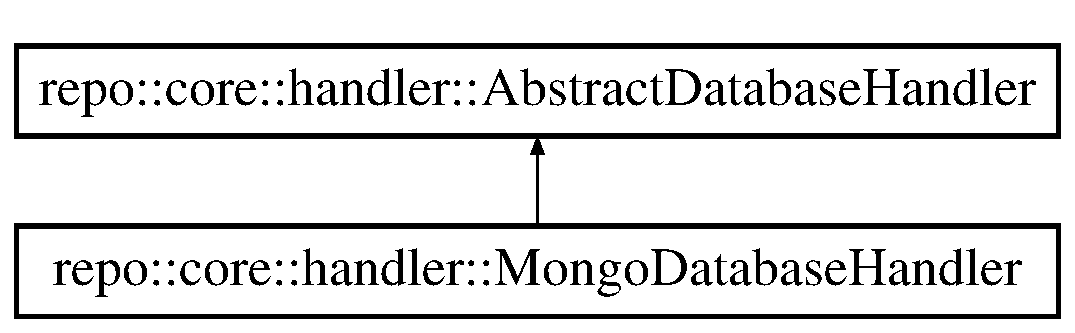
\includegraphics[height=2.000000cm]{classrepo_1_1core_1_1handler_1_1_abstract_database_handler}
\end{center}
\end{figure}
\subsection*{Public Member Functions}
\begin{DoxyCompactItemize}
\item 
virtual \hyperlink{classrepo_1_1core_1_1handler_1_1_abstract_database_handler_a3aec08171736ff99191feaa32f64e7a0}{$\sim$\+Abstract\+Database\+Handler} ()
\item 
uint64\+\_\+t \hyperlink{classrepo_1_1core_1_1handler_1_1_abstract_database_handler_a14ef2fe2413faac9eecbeba2f83ec0d4}{document\+Size\+Limit} ()
\item 
virtual uint64\+\_\+t \hyperlink{classrepo_1_1core_1_1handler_1_1_abstract_database_handler_a862cb79b547fbd5a524a2f75ae114907}{count\+Items\+In\+Collection} (const std\+::string \&database, const std\+::string \&collection, std\+::string \&err\+Msg)=0
\item 
virtual std\+::vector$<$ \hyperlink{classrepo_1_1core_1_1model_1_1_repo_b_s_o_n}{repo\+::core\+::model\+::\+Repo\+B\+S\+O\+N} $>$ \hyperlink{classrepo_1_1core_1_1handler_1_1_abstract_database_handler_abbd7b86134fc60822b2ae6b9933624ca}{get\+All\+From\+Collection\+Tailable} (const std\+::string \&database, const std\+::string \&collection, const uint64\+\_\+t \&skip=0, const uint32\+\_\+t \&limit=0, const std\+::list$<$ std\+::string $>$ \&fields=std\+::list$<$ std\+::string $>$(), const std\+::string \&sort\+Field=std\+::string(), const int \&sort\+Order=-\/1)=0
\item 
virtual std\+::list$<$ std\+::string $>$ \hyperlink{classrepo_1_1core_1_1handler_1_1_abstract_database_handler_ac2007585bdd3c625fd02e61e305f3229}{get\+Collections} (const std\+::string \&database)=0
\item 
virtual \hyperlink{classrepo_1_1core_1_1model_1_1_collection_stats}{repo\+::core\+::model\+::\+Collection\+Stats} \hyperlink{classrepo_1_1core_1_1handler_1_1_abstract_database_handler_a4b1991d2ea832bebab6ffaac81d12350}{get\+Collection\+Stats} (const std\+::string \&database, const std\+::string \&collection, std\+::string \&err\+Msg)=0
\item 
virtual std\+::list$<$ std\+::string $>$ \hyperlink{classrepo_1_1core_1_1handler_1_1_abstract_database_handler_a68d7749c249111292974a00822a0e637}{get\+Databases} (const bool \&sorted=true)=0
\item 
virtual std\+::map$<$ std\+::string, std\+::list$<$ std\+::string $>$ $>$ \hyperlink{classrepo_1_1core_1_1handler_1_1_abstract_database_handler_ab7a050e1fac238a15d782efac324aaf4}{get\+Databases\+With\+Projects} (const std\+::list$<$ std\+::string $>$ \&databases, const std\+::string \&project\+Ext=\char`\"{}scene\char`\"{})=0
\item 
virtual std\+::list$<$ std\+::string $>$ \hyperlink{classrepo_1_1core_1_1handler_1_1_abstract_database_handler_a1470a0e85e9b219d44567b38132e719d}{get\+Projects} (const std\+::string \&database, const std\+::string \&project\+Ext)=0
\item 
virtual std\+::list$<$ std\+::string $>$ \hyperlink{classrepo_1_1core_1_1handler_1_1_abstract_database_handler_a144930566b6a49042b2f17300716ec0f}{get\+Admin\+Database\+Roles} ()=0
\item 
virtual std\+::list$<$ std\+::string $>$ \hyperlink{classrepo_1_1core_1_1handler_1_1_abstract_database_handler_af626a68ca19507b2ff02b52cf1194110}{get\+Standard\+Database\+Roles} ()=0
\item 
virtual void \hyperlink{classrepo_1_1core_1_1handler_1_1_abstract_database_handler_a55a28fe47b164cb4578cb4e682759439}{create\+Collection} (const std\+::string \&database, const std\+::string \&name)=0
\item 
virtual bool \hyperlink{classrepo_1_1core_1_1handler_1_1_abstract_database_handler_a46cffb1fa82f8f5265727ed04cdbfe30}{insert\+Document} (const std\+::string \&database, const std\+::string \&collection, const \hyperlink{classrepo_1_1core_1_1model_1_1_repo_b_s_o_n}{repo\+::core\+::model\+::\+Repo\+B\+S\+O\+N} \&obj, std\+::string \&err\+Msg)=0
\item 
virtual bool \hyperlink{classrepo_1_1core_1_1handler_1_1_abstract_database_handler_a83ad94918c161f5511abab7cac99a5f2}{insert\+Raw\+File} (const std\+::string \&database, const std\+::string \&collection, const std\+::string \&file\+Name, const std\+::vector$<$ uint8\+\_\+t $>$ \&bin, std\+::string \&err\+Msg, const std\+::string \&content\+Type=\char`\"{}binary/octet-\/stream\char`\"{})=0
\item 
virtual bool \hyperlink{classrepo_1_1core_1_1handler_1_1_abstract_database_handler_a93ddebde4c94ca15d0146463e506d063}{insert\+Role} (const \hyperlink{classrepo_1_1core_1_1model_1_1_repo_role}{repo\+::core\+::model\+::\+Repo\+Role} \&role, std\+::string \&errmsg)=0
\item 
virtual bool \hyperlink{classrepo_1_1core_1_1handler_1_1_abstract_database_handler_a1264f8caf3b3e968632dca720002dab6}{insert\+User} (const \hyperlink{classrepo_1_1core_1_1model_1_1_repo_user}{repo\+::core\+::model\+::\+Repo\+User} \&user, std\+::string \&errmsg)=0
\item 
virtual bool \hyperlink{classrepo_1_1core_1_1handler_1_1_abstract_database_handler_a5387adf2593b59bdca51290270299b16}{upsert\+Document} (const std\+::string \&database, const std\+::string \&collection, const \hyperlink{classrepo_1_1core_1_1model_1_1_repo_b_s_o_n}{repo\+::core\+::model\+::\+Repo\+B\+S\+O\+N} \&obj, const bool \&overwrite, std\+::string \&err\+Msg)=0
\item 
virtual bool \hyperlink{classrepo_1_1core_1_1handler_1_1_abstract_database_handler_ab268b2a7d4e0ae0499d016d3311767e7}{drop\+Collection} (const std\+::string \&database, const std\+::string \&collection, std\+::string \&err\+Msg)=0
\item 
virtual bool \hyperlink{classrepo_1_1core_1_1handler_1_1_abstract_database_handler_ad169812ef62d6d21a02d5545633492c0}{drop\+Database} (const std\+::string \&database, std\+::string \&err\+Msg)=0
\item 
virtual bool \hyperlink{classrepo_1_1core_1_1handler_1_1_abstract_database_handler_a189685c88cbadb3f239829d65d4dcb3b}{drop\+Document} (const \hyperlink{classrepo_1_1core_1_1model_1_1_repo_b_s_o_n}{repo\+::core\+::model\+::\+Repo\+B\+S\+O\+N} bson, const std\+::string \&database, const std\+::string \&collection, std\+::string \&err\+Msg)=0
\item 
virtual bool \hyperlink{classrepo_1_1core_1_1handler_1_1_abstract_database_handler_a8b8cdc64a009b872ece09a4f91cdad0c}{drop\+Documents} (const \hyperlink{classrepo_1_1core_1_1model_1_1_repo_b_s_o_n}{repo\+::core\+::model\+::\+Repo\+B\+S\+O\+N} criteria, const std\+::string \&database, const std\+::string \&collection, std\+::string \&err\+Msg)=0
\item 
virtual bool \hyperlink{classrepo_1_1core_1_1handler_1_1_abstract_database_handler_a4806eb978154c4b4bab85eb99d457318}{drop\+Raw\+File} (const std\+::string \&database, const std\+::string \&collection, const std\+::string \&file\+Name, std\+::string \&err\+Msg)=0
\item 
virtual bool \hyperlink{classrepo_1_1core_1_1handler_1_1_abstract_database_handler_a65822a2183bec303c08008fadb1d17d2}{drop\+Role} (const \hyperlink{classrepo_1_1core_1_1model_1_1_repo_role}{repo\+::core\+::model\+::\+Repo\+Role} \&role, std\+::string \&errmsg)=0
\item 
virtual bool \hyperlink{classrepo_1_1core_1_1handler_1_1_abstract_database_handler_a07bd15002e4c23c138a39d3b47af3882}{drop\+User} (const \hyperlink{classrepo_1_1core_1_1model_1_1_repo_user}{repo\+::core\+::model\+::\+Repo\+User} \&user, std\+::string \&errmsg)=0
\item 
virtual bool \hyperlink{classrepo_1_1core_1_1handler_1_1_abstract_database_handler_a7253300babe9db40658616b9c227c9e7}{update\+Role} (const \hyperlink{classrepo_1_1core_1_1model_1_1_repo_role}{repo\+::core\+::model\+::\+Repo\+Role} \&role, std\+::string \&errmsg)=0
\item 
virtual bool \hyperlink{classrepo_1_1core_1_1handler_1_1_abstract_database_handler_a28b9829e0888e2cb4568f6bb13c95d93}{update\+User} (const \hyperlink{classrepo_1_1core_1_1model_1_1_repo_user}{repo\+::core\+::model\+::\+Repo\+User} \&user, std\+::string \&errmsg)=0
\item 
virtual std\+::vector$<$ \hyperlink{classrepo_1_1core_1_1model_1_1_repo_b_s_o_n}{repo\+::core\+::model\+::\+Repo\+B\+S\+O\+N} $>$ \hyperlink{classrepo_1_1core_1_1handler_1_1_abstract_database_handler_ad964d9c80fcddf1444edcf7021c81e50}{find\+All\+By\+Criteria} (const std\+::string \&database, const std\+::string \&collection, const \hyperlink{classrepo_1_1core_1_1model_1_1_repo_b_s_o_n}{repo\+::core\+::model\+::\+Repo\+B\+S\+O\+N} \&criteria)=0
\item 
virtual \hyperlink{classrepo_1_1core_1_1model_1_1_repo_b_s_o_n}{repo\+::core\+::model\+::\+Repo\+B\+S\+O\+N} \hyperlink{classrepo_1_1core_1_1handler_1_1_abstract_database_handler_a321cc0160469e94b12fa5fe800c6c1c5}{find\+One\+By\+Criteria} (const std\+::string \&database, const std\+::string \&collection, const \hyperlink{classrepo_1_1core_1_1model_1_1_repo_b_s_o_n}{repo\+::core\+::model\+::\+Repo\+B\+S\+O\+N} \&criteria, const std\+::string \&sort\+Field=\char`\"{}\char`\"{})=0
\item 
virtual std\+::vector$<$ \hyperlink{classrepo_1_1core_1_1model_1_1_repo_b_s_o_n}{repo\+::core\+::model\+::\+Repo\+B\+S\+O\+N} $>$ \hyperlink{classrepo_1_1core_1_1handler_1_1_abstract_database_handler_ad62823283064682c08acd1bd6f1414f8}{find\+All\+By\+Unique\+I\+Ds} (const std\+::string \&database, const std\+::string \&collection, const \hyperlink{classrepo_1_1core_1_1model_1_1_repo_b_s_o_n}{repo\+::core\+::model\+::\+Repo\+B\+S\+O\+N} \&uuid)=0
\item 
virtual \hyperlink{classrepo_1_1core_1_1model_1_1_repo_b_s_o_n}{repo\+::core\+::model\+::\+Repo\+B\+S\+O\+N} \hyperlink{classrepo_1_1core_1_1handler_1_1_abstract_database_handler_ab83477a74036a6e608620ab53b67df58}{find\+One\+By\+Shared\+I\+D} (const std\+::string \&database, const std\+::string \&collection, const repo\+U\+U\+I\+D \&uuid, const std\+::string \&sort\+Field)=0
\item 
virtual \hyperlink{classrepo_1_1core_1_1model_1_1_repo_b_s_o_n}{repo\+::core\+::model\+::\+Repo\+B\+S\+O\+N} \hyperlink{classrepo_1_1core_1_1handler_1_1_abstract_database_handler_af6cae49e44df081b5895cbf7b7ff6652}{find\+One\+By\+Unique\+I\+D} (const std\+::string \&database, const std\+::string \&collection, const repo\+U\+U\+I\+D \&uuid)=0
\item 
virtual std\+::vector$<$ uint8\+\_\+t $>$ \hyperlink{classrepo_1_1core_1_1handler_1_1_abstract_database_handler_af3d3e2d5d3013ab51675247b202ed488}{get\+Raw\+File} (const std\+::string \&database, const std\+::string \&collection, const std\+::string \&fname)=0
\end{DoxyCompactItemize}
\subsection*{Protected Member Functions}
\begin{DoxyCompactItemize}
\item 
\hyperlink{classrepo_1_1core_1_1handler_1_1_abstract_database_handler_a109197fc892387d988639be7ea456e63}{Abstract\+Database\+Handler} (uint64\+\_\+t size)
\end{DoxyCompactItemize}
\subsection*{Protected Attributes}
\begin{DoxyCompactItemize}
\item 
\hypertarget{classrepo_1_1core_1_1handler_1_1_abstract_database_handler_a867b31d303df31942a82becdc0c76b7e}{}const uint64\+\_\+t {\bfseries max\+Document\+Size}\label{classrepo_1_1core_1_1handler_1_1_abstract_database_handler_a867b31d303df31942a82becdc0c76b7e}

\end{DoxyCompactItemize}


\subsection{Constructor \& Destructor Documentation}
\hypertarget{classrepo_1_1core_1_1handler_1_1_abstract_database_handler_a3aec08171736ff99191feaa32f64e7a0}{}\index{repo\+::core\+::handler\+::\+Abstract\+Database\+Handler@{repo\+::core\+::handler\+::\+Abstract\+Database\+Handler}!````~Abstract\+Database\+Handler@{$\sim$\+Abstract\+Database\+Handler}}
\index{````~Abstract\+Database\+Handler@{$\sim$\+Abstract\+Database\+Handler}!repo\+::core\+::handler\+::\+Abstract\+Database\+Handler@{repo\+::core\+::handler\+::\+Abstract\+Database\+Handler}}
\subsubsection[{$\sim$\+Abstract\+Database\+Handler}]{\setlength{\rightskip}{0pt plus 5cm}virtual repo\+::core\+::handler\+::\+Abstract\+Database\+Handler\+::$\sim$\+Abstract\+Database\+Handler (
\begin{DoxyParamCaption}
{}
\end{DoxyParamCaption}
)\hspace{0.3cm}{\ttfamily [inline]}, {\ttfamily [virtual]}}\label{classrepo_1_1core_1_1handler_1_1_abstract_database_handler_a3aec08171736ff99191feaa32f64e7a0}
A Deconstructor \hypertarget{classrepo_1_1core_1_1handler_1_1_abstract_database_handler_a109197fc892387d988639be7ea456e63}{}\index{repo\+::core\+::handler\+::\+Abstract\+Database\+Handler@{repo\+::core\+::handler\+::\+Abstract\+Database\+Handler}!Abstract\+Database\+Handler@{Abstract\+Database\+Handler}}
\index{Abstract\+Database\+Handler@{Abstract\+Database\+Handler}!repo\+::core\+::handler\+::\+Abstract\+Database\+Handler@{repo\+::core\+::handler\+::\+Abstract\+Database\+Handler}}
\subsubsection[{Abstract\+Database\+Handler}]{\setlength{\rightskip}{0pt plus 5cm}repo\+::core\+::handler\+::\+Abstract\+Database\+Handler\+::\+Abstract\+Database\+Handler (
\begin{DoxyParamCaption}
\item[{uint64\+\_\+t}]{size}
\end{DoxyParamCaption}
)\hspace{0.3cm}{\ttfamily [inline]}, {\ttfamily [protected]}}\label{classrepo_1_1core_1_1handler_1_1_abstract_database_handler_a109197fc892387d988639be7ea456e63}
Default constructor 
\begin{DoxyParams}{Parameters}
{\em size} & maximum size of documents(records) in bytes \\
\hline
\end{DoxyParams}


\subsection{Member Function Documentation}
\hypertarget{classrepo_1_1core_1_1handler_1_1_abstract_database_handler_a862cb79b547fbd5a524a2f75ae114907}{}\index{repo\+::core\+::handler\+::\+Abstract\+Database\+Handler@{repo\+::core\+::handler\+::\+Abstract\+Database\+Handler}!count\+Items\+In\+Collection@{count\+Items\+In\+Collection}}
\index{count\+Items\+In\+Collection@{count\+Items\+In\+Collection}!repo\+::core\+::handler\+::\+Abstract\+Database\+Handler@{repo\+::core\+::handler\+::\+Abstract\+Database\+Handler}}
\subsubsection[{count\+Items\+In\+Collection}]{\setlength{\rightskip}{0pt plus 5cm}virtual uint64\+\_\+t repo\+::core\+::handler\+::\+Abstract\+Database\+Handler\+::count\+Items\+In\+Collection (
\begin{DoxyParamCaption}
\item[{const std\+::string \&}]{database, }
\item[{const std\+::string \&}]{collection, }
\item[{std\+::string \&}]{err\+Msg}
\end{DoxyParamCaption}
)\hspace{0.3cm}{\ttfamily [pure virtual]}}\label{classrepo_1_1core_1_1handler_1_1_abstract_database_handler_a862cb79b547fbd5a524a2f75ae114907}
Generates a B\+S\+O\+N object containing user credentials 
\begin{DoxyParams}{Parameters}
{\em username} & user name for authentication \\
\hline
{\em password} & password of the user \\
\hline
{\em pw\+Digested} & true if pw is digested \\
\hline
\end{DoxyParams}
\begin{DoxyReturn}{Returns}
returns the constructed B\+S\+O\+N object, or 0 if username is empty Count the number of documents within the collection 
\end{DoxyReturn}

\begin{DoxyParams}{Parameters}
{\em database} & name of database \\
\hline
{\em collection} & name of collection \\
\hline
{\em err\+Msg} & err\+Msg if failed \\
\hline
\end{DoxyParams}
\begin{DoxyReturn}{Returns}
number of documents within the specified collection 
\end{DoxyReturn}


Implemented in \hyperlink{classrepo_1_1core_1_1handler_1_1_mongo_database_handler_ad69882e8c3573be494c5b6eca6a53827}{repo\+::core\+::handler\+::\+Mongo\+Database\+Handler}.

\hypertarget{classrepo_1_1core_1_1handler_1_1_abstract_database_handler_a55a28fe47b164cb4578cb4e682759439}{}\index{repo\+::core\+::handler\+::\+Abstract\+Database\+Handler@{repo\+::core\+::handler\+::\+Abstract\+Database\+Handler}!create\+Collection@{create\+Collection}}
\index{create\+Collection@{create\+Collection}!repo\+::core\+::handler\+::\+Abstract\+Database\+Handler@{repo\+::core\+::handler\+::\+Abstract\+Database\+Handler}}
\subsubsection[{create\+Collection}]{\setlength{\rightskip}{0pt plus 5cm}virtual void repo\+::core\+::handler\+::\+Abstract\+Database\+Handler\+::create\+Collection (
\begin{DoxyParamCaption}
\item[{const std\+::string \&}]{database, }
\item[{const std\+::string \&}]{name}
\end{DoxyParamCaption}
)\hspace{0.3cm}{\ttfamily [pure virtual]}}\label{classrepo_1_1core_1_1handler_1_1_abstract_database_handler_a55a28fe47b164cb4578cb4e682759439}
Create a collection with the name specified 
\begin{DoxyParams}{Parameters}
{\em database} & name of the database \\
\hline
{\em name} & name of the collection \\
\hline
\end{DoxyParams}


Implemented in \hyperlink{classrepo_1_1core_1_1handler_1_1_mongo_database_handler_abeaad0e73b0e274755e7ee2baab002ae}{repo\+::core\+::handler\+::\+Mongo\+Database\+Handler}.

\hypertarget{classrepo_1_1core_1_1handler_1_1_abstract_database_handler_a14ef2fe2413faac9eecbeba2f83ec0d4}{}\index{repo\+::core\+::handler\+::\+Abstract\+Database\+Handler@{repo\+::core\+::handler\+::\+Abstract\+Database\+Handler}!document\+Size\+Limit@{document\+Size\+Limit}}
\index{document\+Size\+Limit@{document\+Size\+Limit}!repo\+::core\+::handler\+::\+Abstract\+Database\+Handler@{repo\+::core\+::handler\+::\+Abstract\+Database\+Handler}}
\subsubsection[{document\+Size\+Limit}]{\setlength{\rightskip}{0pt plus 5cm}uint64\+\_\+t repo\+::core\+::handler\+::\+Abstract\+Database\+Handler\+::document\+Size\+Limit (
\begin{DoxyParamCaption}
{}
\end{DoxyParamCaption}
)\hspace{0.3cm}{\ttfamily [inline]}}\label{classrepo_1_1core_1_1handler_1_1_abstract_database_handler_a14ef2fe2413faac9eecbeba2f83ec0d4}
returns the size limit of each document(record) in bytes \begin{DoxyReturn}{Returns}
returns size limit in bytes. 
\end{DoxyReturn}
\hypertarget{classrepo_1_1core_1_1handler_1_1_abstract_database_handler_ab268b2a7d4e0ae0499d016d3311767e7}{}\index{repo\+::core\+::handler\+::\+Abstract\+Database\+Handler@{repo\+::core\+::handler\+::\+Abstract\+Database\+Handler}!drop\+Collection@{drop\+Collection}}
\index{drop\+Collection@{drop\+Collection}!repo\+::core\+::handler\+::\+Abstract\+Database\+Handler@{repo\+::core\+::handler\+::\+Abstract\+Database\+Handler}}
\subsubsection[{drop\+Collection}]{\setlength{\rightskip}{0pt plus 5cm}virtual bool repo\+::core\+::handler\+::\+Abstract\+Database\+Handler\+::drop\+Collection (
\begin{DoxyParamCaption}
\item[{const std\+::string \&}]{database, }
\item[{const std\+::string \&}]{collection, }
\item[{std\+::string \&}]{err\+Msg}
\end{DoxyParamCaption}
)\hspace{0.3cm}{\ttfamily [pure virtual]}}\label{classrepo_1_1core_1_1handler_1_1_abstract_database_handler_ab268b2a7d4e0ae0499d016d3311767e7}
Remove a collection from the database 
\begin{DoxyParams}{Parameters}
{\em database} & the database the collection resides in \\
\hline
{\em collection} & name of the collection to drop \\
\hline
{\em err\+Msg} & name of the collection to drop \\
\hline
\end{DoxyParams}


Implemented in \hyperlink{classrepo_1_1core_1_1handler_1_1_mongo_database_handler_a7c4cdb628a1b3c59caba6b397fe20375}{repo\+::core\+::handler\+::\+Mongo\+Database\+Handler}.

\hypertarget{classrepo_1_1core_1_1handler_1_1_abstract_database_handler_ad169812ef62d6d21a02d5545633492c0}{}\index{repo\+::core\+::handler\+::\+Abstract\+Database\+Handler@{repo\+::core\+::handler\+::\+Abstract\+Database\+Handler}!drop\+Database@{drop\+Database}}
\index{drop\+Database@{drop\+Database}!repo\+::core\+::handler\+::\+Abstract\+Database\+Handler@{repo\+::core\+::handler\+::\+Abstract\+Database\+Handler}}
\subsubsection[{drop\+Database}]{\setlength{\rightskip}{0pt plus 5cm}virtual bool repo\+::core\+::handler\+::\+Abstract\+Database\+Handler\+::drop\+Database (
\begin{DoxyParamCaption}
\item[{const std\+::string \&}]{database, }
\item[{std\+::string \&}]{err\+Msg}
\end{DoxyParamCaption}
)\hspace{0.3cm}{\ttfamily [pure virtual]}}\label{classrepo_1_1core_1_1handler_1_1_abstract_database_handler_ad169812ef62d6d21a02d5545633492c0}
Remove a database from the database instance 
\begin{DoxyParams}{Parameters}
{\em database} & name of the database to drop \\
\hline
{\em err\+Msg} & name of the database to drop \\
\hline
\end{DoxyParams}


Implemented in \hyperlink{classrepo_1_1core_1_1handler_1_1_mongo_database_handler_ac982e4d73ee5c69d333030437eebabf6}{repo\+::core\+::handler\+::\+Mongo\+Database\+Handler}.

\hypertarget{classrepo_1_1core_1_1handler_1_1_abstract_database_handler_a189685c88cbadb3f239829d65d4dcb3b}{}\index{repo\+::core\+::handler\+::\+Abstract\+Database\+Handler@{repo\+::core\+::handler\+::\+Abstract\+Database\+Handler}!drop\+Document@{drop\+Document}}
\index{drop\+Document@{drop\+Document}!repo\+::core\+::handler\+::\+Abstract\+Database\+Handler@{repo\+::core\+::handler\+::\+Abstract\+Database\+Handler}}
\subsubsection[{drop\+Document}]{\setlength{\rightskip}{0pt plus 5cm}virtual bool repo\+::core\+::handler\+::\+Abstract\+Database\+Handler\+::drop\+Document (
\begin{DoxyParamCaption}
\item[{const {\bf repo\+::core\+::model\+::\+Repo\+B\+S\+O\+N}}]{bson, }
\item[{const std\+::string \&}]{database, }
\item[{const std\+::string \&}]{collection, }
\item[{std\+::string \&}]{err\+Msg}
\end{DoxyParamCaption}
)\hspace{0.3cm}{\ttfamily [pure virtual]}}\label{classrepo_1_1core_1_1handler_1_1_abstract_database_handler_a189685c88cbadb3f239829d65d4dcb3b}
Remove a document from the mongo database 
\begin{DoxyParams}{Parameters}
{\em bson} & document to remove \\
\hline
{\em database} & the database the collection resides in \\
\hline
{\em collection} & name of the collection the document is in \\
\hline
{\em err\+Msg} & name of the database to drop \\
\hline
\end{DoxyParams}


Implemented in \hyperlink{classrepo_1_1core_1_1handler_1_1_mongo_database_handler_a7e1a68ada64088e53ded91c738fadcd6}{repo\+::core\+::handler\+::\+Mongo\+Database\+Handler}.

\hypertarget{classrepo_1_1core_1_1handler_1_1_abstract_database_handler_a8b8cdc64a009b872ece09a4f91cdad0c}{}\index{repo\+::core\+::handler\+::\+Abstract\+Database\+Handler@{repo\+::core\+::handler\+::\+Abstract\+Database\+Handler}!drop\+Documents@{drop\+Documents}}
\index{drop\+Documents@{drop\+Documents}!repo\+::core\+::handler\+::\+Abstract\+Database\+Handler@{repo\+::core\+::handler\+::\+Abstract\+Database\+Handler}}
\subsubsection[{drop\+Documents}]{\setlength{\rightskip}{0pt plus 5cm}virtual bool repo\+::core\+::handler\+::\+Abstract\+Database\+Handler\+::drop\+Documents (
\begin{DoxyParamCaption}
\item[{const {\bf repo\+::core\+::model\+::\+Repo\+B\+S\+O\+N}}]{criteria, }
\item[{const std\+::string \&}]{database, }
\item[{const std\+::string \&}]{collection, }
\item[{std\+::string \&}]{err\+Msg}
\end{DoxyParamCaption}
)\hspace{0.3cm}{\ttfamily [pure virtual]}}\label{classrepo_1_1core_1_1handler_1_1_abstract_database_handler_a8b8cdc64a009b872ece09a4f91cdad0c}
Remove all documents satisfying a certain criteria 
\begin{DoxyParams}{Parameters}
{\em criteria} & document to remove \\
\hline
{\em database} & the database the collection resides in \\
\hline
{\em collection} & name of the collection the document is in \\
\hline
{\em err\+Msg} & name of the database to drop \\
\hline
\end{DoxyParams}


Implemented in \hyperlink{classrepo_1_1core_1_1handler_1_1_mongo_database_handler_a15263c0497c215798ac7398ff89bb4d3}{repo\+::core\+::handler\+::\+Mongo\+Database\+Handler}.

\hypertarget{classrepo_1_1core_1_1handler_1_1_abstract_database_handler_a4806eb978154c4b4bab85eb99d457318}{}\index{repo\+::core\+::handler\+::\+Abstract\+Database\+Handler@{repo\+::core\+::handler\+::\+Abstract\+Database\+Handler}!drop\+Raw\+File@{drop\+Raw\+File}}
\index{drop\+Raw\+File@{drop\+Raw\+File}!repo\+::core\+::handler\+::\+Abstract\+Database\+Handler@{repo\+::core\+::handler\+::\+Abstract\+Database\+Handler}}
\subsubsection[{drop\+Raw\+File}]{\setlength{\rightskip}{0pt plus 5cm}virtual bool repo\+::core\+::handler\+::\+Abstract\+Database\+Handler\+::drop\+Raw\+File (
\begin{DoxyParamCaption}
\item[{const std\+::string \&}]{database, }
\item[{const std\+::string \&}]{collection, }
\item[{const std\+::string \&}]{file\+Name, }
\item[{std\+::string \&}]{err\+Msg}
\end{DoxyParamCaption}
)\hspace{0.3cm}{\ttfamily [pure virtual]}}\label{classrepo_1_1core_1_1handler_1_1_abstract_database_handler_a4806eb978154c4b4bab85eb99d457318}
Remove a file from raw file storage (grid\+F\+S) 
\begin{DoxyParams}{Parameters}
{\em database} & the database the collection resides in \\
\hline
{\em collection} & name of the collection the document is in \\
\hline
{\em filename} & name of the file \\
\hline
{\em err\+Msg} & name of the database to drop \\
\hline
\end{DoxyParams}


Implemented in \hyperlink{classrepo_1_1core_1_1handler_1_1_mongo_database_handler_a847556c14e85da5e17f8d21c70ab23d0}{repo\+::core\+::handler\+::\+Mongo\+Database\+Handler}.

\hypertarget{classrepo_1_1core_1_1handler_1_1_abstract_database_handler_a65822a2183bec303c08008fadb1d17d2}{}\index{repo\+::core\+::handler\+::\+Abstract\+Database\+Handler@{repo\+::core\+::handler\+::\+Abstract\+Database\+Handler}!drop\+Role@{drop\+Role}}
\index{drop\+Role@{drop\+Role}!repo\+::core\+::handler\+::\+Abstract\+Database\+Handler@{repo\+::core\+::handler\+::\+Abstract\+Database\+Handler}}
\subsubsection[{drop\+Role}]{\setlength{\rightskip}{0pt plus 5cm}virtual bool repo\+::core\+::handler\+::\+Abstract\+Database\+Handler\+::drop\+Role (
\begin{DoxyParamCaption}
\item[{const {\bf repo\+::core\+::model\+::\+Repo\+Role} \&}]{role, }
\item[{std\+::string \&}]{errmsg}
\end{DoxyParamCaption}
)\hspace{0.3cm}{\ttfamily [pure virtual]}}\label{classrepo_1_1core_1_1handler_1_1_abstract_database_handler_a65822a2183bec303c08008fadb1d17d2}
Remove a role from the database 
\begin{DoxyParams}{Parameters}
{\em role} & user bson to remove \\
\hline
{\em errmsg} & error message \\
\hline
\end{DoxyParams}
\begin{DoxyReturn}{Returns}
returns true upon success 
\end{DoxyReturn}


Implemented in \hyperlink{classrepo_1_1core_1_1handler_1_1_mongo_database_handler_ade2b069da1314566c63a48a3b61ad451}{repo\+::core\+::handler\+::\+Mongo\+Database\+Handler}.

\hypertarget{classrepo_1_1core_1_1handler_1_1_abstract_database_handler_a07bd15002e4c23c138a39d3b47af3882}{}\index{repo\+::core\+::handler\+::\+Abstract\+Database\+Handler@{repo\+::core\+::handler\+::\+Abstract\+Database\+Handler}!drop\+User@{drop\+User}}
\index{drop\+User@{drop\+User}!repo\+::core\+::handler\+::\+Abstract\+Database\+Handler@{repo\+::core\+::handler\+::\+Abstract\+Database\+Handler}}
\subsubsection[{drop\+User}]{\setlength{\rightskip}{0pt plus 5cm}virtual bool repo\+::core\+::handler\+::\+Abstract\+Database\+Handler\+::drop\+User (
\begin{DoxyParamCaption}
\item[{const {\bf repo\+::core\+::model\+::\+Repo\+User} \&}]{user, }
\item[{std\+::string \&}]{errmsg}
\end{DoxyParamCaption}
)\hspace{0.3cm}{\ttfamily [pure virtual]}}\label{classrepo_1_1core_1_1handler_1_1_abstract_database_handler_a07bd15002e4c23c138a39d3b47af3882}
Remove a user from the database 
\begin{DoxyParams}{Parameters}
{\em user} & user bson to remove \\
\hline
{\em errmsg} & error message \\
\hline
\end{DoxyParams}
\begin{DoxyReturn}{Returns}
returns true upon success 
\end{DoxyReturn}


Implemented in \hyperlink{classrepo_1_1core_1_1handler_1_1_mongo_database_handler_ad5e1716d61ffe74086453ae4d0bbad24}{repo\+::core\+::handler\+::\+Mongo\+Database\+Handler}.

\hypertarget{classrepo_1_1core_1_1handler_1_1_abstract_database_handler_ad964d9c80fcddf1444edcf7021c81e50}{}\index{repo\+::core\+::handler\+::\+Abstract\+Database\+Handler@{repo\+::core\+::handler\+::\+Abstract\+Database\+Handler}!find\+All\+By\+Criteria@{find\+All\+By\+Criteria}}
\index{find\+All\+By\+Criteria@{find\+All\+By\+Criteria}!repo\+::core\+::handler\+::\+Abstract\+Database\+Handler@{repo\+::core\+::handler\+::\+Abstract\+Database\+Handler}}
\subsubsection[{find\+All\+By\+Criteria}]{\setlength{\rightskip}{0pt plus 5cm}virtual std\+::vector$<${\bf repo\+::core\+::model\+::\+Repo\+B\+S\+O\+N}$>$ repo\+::core\+::handler\+::\+Abstract\+Database\+Handler\+::find\+All\+By\+Criteria (
\begin{DoxyParamCaption}
\item[{const std\+::string \&}]{database, }
\item[{const std\+::string \&}]{collection, }
\item[{const {\bf repo\+::core\+::model\+::\+Repo\+B\+S\+O\+N} \&}]{criteria}
\end{DoxyParamCaption}
)\hspace{0.3cm}{\ttfamily [pure virtual]}}\label{classrepo_1_1core_1_1handler_1_1_abstract_database_handler_ad964d9c80fcddf1444edcf7021c81e50}
Given a search criteria, find all the documents that passes this query 
\begin{DoxyParams}{Parameters}
{\em database} & name of database \\
\hline
{\em collection} & name of collection \\
\hline
{\em criteria} & search criteria in a bson object \\
\hline
\end{DoxyParams}
\begin{DoxyReturn}{Returns}
a vector of Repo\+B\+S\+O\+N objects satisfy the given criteria 
\end{DoxyReturn}


Implemented in \hyperlink{classrepo_1_1core_1_1handler_1_1_mongo_database_handler_af8bc6c5531e6669b9ac278c6fc64ec3e}{repo\+::core\+::handler\+::\+Mongo\+Database\+Handler}.

\hypertarget{classrepo_1_1core_1_1handler_1_1_abstract_database_handler_ad62823283064682c08acd1bd6f1414f8}{}\index{repo\+::core\+::handler\+::\+Abstract\+Database\+Handler@{repo\+::core\+::handler\+::\+Abstract\+Database\+Handler}!find\+All\+By\+Unique\+I\+Ds@{find\+All\+By\+Unique\+I\+Ds}}
\index{find\+All\+By\+Unique\+I\+Ds@{find\+All\+By\+Unique\+I\+Ds}!repo\+::core\+::handler\+::\+Abstract\+Database\+Handler@{repo\+::core\+::handler\+::\+Abstract\+Database\+Handler}}
\subsubsection[{find\+All\+By\+Unique\+I\+Ds}]{\setlength{\rightskip}{0pt plus 5cm}virtual std\+::vector$<${\bf repo\+::core\+::model\+::\+Repo\+B\+S\+O\+N}$>$ repo\+::core\+::handler\+::\+Abstract\+Database\+Handler\+::find\+All\+By\+Unique\+I\+Ds (
\begin{DoxyParamCaption}
\item[{const std\+::string \&}]{database, }
\item[{const std\+::string \&}]{collection, }
\item[{const {\bf repo\+::core\+::model\+::\+Repo\+B\+S\+O\+N} \&}]{uuid}
\end{DoxyParamCaption}
)\hspace{0.3cm}{\ttfamily [pure virtual]}}\label{classrepo_1_1core_1_1handler_1_1_abstract_database_handler_ad62823283064682c08acd1bd6f1414f8}
Given a list of unique I\+Ds, find all the documents associated to them 
\begin{DoxyParams}{Parameters}
{\em name} & of database \\
\hline
{\em name} & of collection \\
\hline
{\em array} & of uuids in a B\+S\+O\+N object \\
\hline
\end{DoxyParams}
\begin{DoxyReturn}{Returns}
a vector of Repo\+B\+S\+O\+N objects associated with the U\+U\+I\+Ds given 
\end{DoxyReturn}


Implemented in \hyperlink{classrepo_1_1core_1_1handler_1_1_mongo_database_handler_a26cca6e23ce8e218fe5c6106bc91425a}{repo\+::core\+::handler\+::\+Mongo\+Database\+Handler}.

\hypertarget{classrepo_1_1core_1_1handler_1_1_abstract_database_handler_a321cc0160469e94b12fa5fe800c6c1c5}{}\index{repo\+::core\+::handler\+::\+Abstract\+Database\+Handler@{repo\+::core\+::handler\+::\+Abstract\+Database\+Handler}!find\+One\+By\+Criteria@{find\+One\+By\+Criteria}}
\index{find\+One\+By\+Criteria@{find\+One\+By\+Criteria}!repo\+::core\+::handler\+::\+Abstract\+Database\+Handler@{repo\+::core\+::handler\+::\+Abstract\+Database\+Handler}}
\subsubsection[{find\+One\+By\+Criteria}]{\setlength{\rightskip}{0pt plus 5cm}virtual {\bf repo\+::core\+::model\+::\+Repo\+B\+S\+O\+N} repo\+::core\+::handler\+::\+Abstract\+Database\+Handler\+::find\+One\+By\+Criteria (
\begin{DoxyParamCaption}
\item[{const std\+::string \&}]{database, }
\item[{const std\+::string \&}]{collection, }
\item[{const {\bf repo\+::core\+::model\+::\+Repo\+B\+S\+O\+N} \&}]{criteria, }
\item[{const std\+::string \&}]{sort\+Field = {\ttfamily \char`\"{}\char`\"{}}}
\end{DoxyParamCaption}
)\hspace{0.3cm}{\ttfamily [pure virtual]}}\label{classrepo_1_1core_1_1handler_1_1_abstract_database_handler_a321cc0160469e94b12fa5fe800c6c1c5}
Given a search criteria, find one documents that passes this query 
\begin{DoxyParams}{Parameters}
{\em database} & name of database \\
\hline
{\em collection} & name of collection \\
\hline
{\em criteria} & search criteria in a bson object \\
\hline
{\em sort\+Field} & field to sort \\
\hline
\end{DoxyParams}
\begin{DoxyReturn}{Returns}
a Repo\+B\+S\+O\+N objects satisfy the given criteria 
\end{DoxyReturn}


Implemented in \hyperlink{classrepo_1_1core_1_1handler_1_1_mongo_database_handler_a9e13fe73ff838e388378d82673964e20}{repo\+::core\+::handler\+::\+Mongo\+Database\+Handler}.

\hypertarget{classrepo_1_1core_1_1handler_1_1_abstract_database_handler_ab83477a74036a6e608620ab53b67df58}{}\index{repo\+::core\+::handler\+::\+Abstract\+Database\+Handler@{repo\+::core\+::handler\+::\+Abstract\+Database\+Handler}!find\+One\+By\+Shared\+I\+D@{find\+One\+By\+Shared\+I\+D}}
\index{find\+One\+By\+Shared\+I\+D@{find\+One\+By\+Shared\+I\+D}!repo\+::core\+::handler\+::\+Abstract\+Database\+Handler@{repo\+::core\+::handler\+::\+Abstract\+Database\+Handler}}
\subsubsection[{find\+One\+By\+Shared\+I\+D}]{\setlength{\rightskip}{0pt plus 5cm}virtual {\bf repo\+::core\+::model\+::\+Repo\+B\+S\+O\+N} repo\+::core\+::handler\+::\+Abstract\+Database\+Handler\+::find\+One\+By\+Shared\+I\+D (
\begin{DoxyParamCaption}
\item[{const std\+::string \&}]{database, }
\item[{const std\+::string \&}]{collection, }
\item[{const repo\+U\+U\+I\+D \&}]{uuid, }
\item[{const std\+::string \&}]{sort\+Field}
\end{DoxyParamCaption}
)\hspace{0.3cm}{\ttfamily [pure virtual]}}\label{classrepo_1_1core_1_1handler_1_1_abstract_database_handler_ab83477a74036a6e608620ab53b67df58}
Retrieves the first document matching given Shared I\+D (S\+I\+D), sorting is descending (newest first) 
\begin{DoxyParams}{Parameters}
{\em database} & name of database \\
\hline
{\em collection} & name of collection \\
\hline
{\em uuid} & share id \\
\hline
{\em field} & field to sort by \\
\hline
\end{DoxyParams}
\begin{DoxyReturn}{Returns}
returns the first matching bson object 
\end{DoxyReturn}


Implemented in \hyperlink{classrepo_1_1core_1_1handler_1_1_mongo_database_handler_aae7c0539fcdbad26c307c9f63877d536}{repo\+::core\+::handler\+::\+Mongo\+Database\+Handler}.

\hypertarget{classrepo_1_1core_1_1handler_1_1_abstract_database_handler_af6cae49e44df081b5895cbf7b7ff6652}{}\index{repo\+::core\+::handler\+::\+Abstract\+Database\+Handler@{repo\+::core\+::handler\+::\+Abstract\+Database\+Handler}!find\+One\+By\+Unique\+I\+D@{find\+One\+By\+Unique\+I\+D}}
\index{find\+One\+By\+Unique\+I\+D@{find\+One\+By\+Unique\+I\+D}!repo\+::core\+::handler\+::\+Abstract\+Database\+Handler@{repo\+::core\+::handler\+::\+Abstract\+Database\+Handler}}
\subsubsection[{find\+One\+By\+Unique\+I\+D}]{\setlength{\rightskip}{0pt plus 5cm}virtual {\bf repo\+::core\+::model\+::\+Repo\+B\+S\+O\+N} repo\+::core\+::handler\+::\+Abstract\+Database\+Handler\+::find\+One\+By\+Unique\+I\+D (
\begin{DoxyParamCaption}
\item[{const std\+::string \&}]{database, }
\item[{const std\+::string \&}]{collection, }
\item[{const repo\+U\+U\+I\+D \&}]{uuid}
\end{DoxyParamCaption}
)\hspace{0.3cm}{\ttfamily [pure virtual]}}\label{classrepo_1_1core_1_1handler_1_1_abstract_database_handler_af6cae49e44df081b5895cbf7b7ff6652}
Retrieves the document matching given Unique I\+D (S\+I\+D), sorting is descending 
\begin{DoxyParams}{Parameters}
{\em database} & name of database \\
\hline
{\em collection} & name of collection \\
\hline
{\em uuid} & share id \\
\hline
\end{DoxyParams}
\begin{DoxyReturn}{Returns}
returns the matching bson object 
\end{DoxyReturn}


Implemented in \hyperlink{classrepo_1_1core_1_1handler_1_1_mongo_database_handler_ac016547468fc0049c859d775e270e17a}{repo\+::core\+::handler\+::\+Mongo\+Database\+Handler}.

\hypertarget{classrepo_1_1core_1_1handler_1_1_abstract_database_handler_a144930566b6a49042b2f17300716ec0f}{}\index{repo\+::core\+::handler\+::\+Abstract\+Database\+Handler@{repo\+::core\+::handler\+::\+Abstract\+Database\+Handler}!get\+Admin\+Database\+Roles@{get\+Admin\+Database\+Roles}}
\index{get\+Admin\+Database\+Roles@{get\+Admin\+Database\+Roles}!repo\+::core\+::handler\+::\+Abstract\+Database\+Handler@{repo\+::core\+::handler\+::\+Abstract\+Database\+Handler}}
\subsubsection[{get\+Admin\+Database\+Roles}]{\setlength{\rightskip}{0pt plus 5cm}virtual std\+::list$<$std\+::string$>$ repo\+::core\+::handler\+::\+Abstract\+Database\+Handler\+::get\+Admin\+Database\+Roles (
\begin{DoxyParamCaption}
{}
\end{DoxyParamCaption}
)\hspace{0.3cm}{\ttfamily [pure virtual]}}\label{classrepo_1_1core_1_1handler_1_1_abstract_database_handler_a144930566b6a49042b2f17300716ec0f}
Return a list of Admin database roles \begin{DoxyReturn}{Returns}
a vector of Admin database roles 
\end{DoxyReturn}


Implemented in \hyperlink{classrepo_1_1core_1_1handler_1_1_mongo_database_handler_afeaa95dcb44d7a1276fa1e90a5987f6d}{repo\+::core\+::handler\+::\+Mongo\+Database\+Handler}.

\hypertarget{classrepo_1_1core_1_1handler_1_1_abstract_database_handler_abbd7b86134fc60822b2ae6b9933624ca}{}\index{repo\+::core\+::handler\+::\+Abstract\+Database\+Handler@{repo\+::core\+::handler\+::\+Abstract\+Database\+Handler}!get\+All\+From\+Collection\+Tailable@{get\+All\+From\+Collection\+Tailable}}
\index{get\+All\+From\+Collection\+Tailable@{get\+All\+From\+Collection\+Tailable}!repo\+::core\+::handler\+::\+Abstract\+Database\+Handler@{repo\+::core\+::handler\+::\+Abstract\+Database\+Handler}}
\subsubsection[{get\+All\+From\+Collection\+Tailable}]{\setlength{\rightskip}{0pt plus 5cm}virtual std\+::vector$<${\bf repo\+::core\+::model\+::\+Repo\+B\+S\+O\+N}$>$ repo\+::core\+::handler\+::\+Abstract\+Database\+Handler\+::get\+All\+From\+Collection\+Tailable (
\begin{DoxyParamCaption}
\item[{const std\+::string \&}]{database, }
\item[{const std\+::string \&}]{collection, }
\item[{const uint64\+\_\+t \&}]{skip = {\ttfamily 0}, }
\item[{const uint32\+\_\+t \&}]{limit = {\ttfamily 0}, }
\item[{const std\+::list$<$ std\+::string $>$ \&}]{fields = {\ttfamily std\+:\+:list$<$~std\+:\+:string~$>$()}, }
\item[{const std\+::string \&}]{sort\+Field = {\ttfamily std\+:\+:string()}, }
\item[{const int \&}]{sort\+Order = {\ttfamily -\/1}}
\end{DoxyParamCaption}
)\hspace{0.3cm}{\ttfamily [pure virtual]}}\label{classrepo_1_1core_1_1handler_1_1_abstract_database_handler_abbd7b86134fc60822b2ae6b9933624ca}
Retrieve documents from a specified collection due to limitations of the transfer protocol this might need to be called multiple times, utilising the skip index to skip the first n items. 
\begin{DoxyParams}{Parameters}
{\em database} & name of database \\
\hline
{\em collection} & name of collection \\
\hline
{\em fields} & fields to get back from the database \\
\hline
{\em sort\+Field} & field to sort upon \\
\hline
{\em sort\+Order} & 1 ascending, -\/1 descending \\
\hline
{\em skip} & specify how many documents to skip \\
\hline
\end{DoxyParams}
\begin{DoxyReturn}{Returns}
list of Repo\+B\+S\+O\+Ns representing the documents 
\end{DoxyReturn}


Implemented in \hyperlink{classrepo_1_1core_1_1handler_1_1_mongo_database_handler_a3083dc4c2983681aa2b356c87bcaeca3}{repo\+::core\+::handler\+::\+Mongo\+Database\+Handler}.

\hypertarget{classrepo_1_1core_1_1handler_1_1_abstract_database_handler_ac2007585bdd3c625fd02e61e305f3229}{}\index{repo\+::core\+::handler\+::\+Abstract\+Database\+Handler@{repo\+::core\+::handler\+::\+Abstract\+Database\+Handler}!get\+Collections@{get\+Collections}}
\index{get\+Collections@{get\+Collections}!repo\+::core\+::handler\+::\+Abstract\+Database\+Handler@{repo\+::core\+::handler\+::\+Abstract\+Database\+Handler}}
\subsubsection[{get\+Collections}]{\setlength{\rightskip}{0pt plus 5cm}virtual std\+::list$<$std\+::string$>$ repo\+::core\+::handler\+::\+Abstract\+Database\+Handler\+::get\+Collections (
\begin{DoxyParamCaption}
\item[{const std\+::string \&}]{database}
\end{DoxyParamCaption}
)\hspace{0.3cm}{\ttfamily [pure virtual]}}\label{classrepo_1_1core_1_1handler_1_1_abstract_database_handler_ac2007585bdd3c625fd02e61e305f3229}
Get a list of all available collections 

Implemented in \hyperlink{classrepo_1_1core_1_1handler_1_1_mongo_database_handler_ad51771cf9bca612634c4e761266c5d32}{repo\+::core\+::handler\+::\+Mongo\+Database\+Handler}.

\hypertarget{classrepo_1_1core_1_1handler_1_1_abstract_database_handler_a4b1991d2ea832bebab6ffaac81d12350}{}\index{repo\+::core\+::handler\+::\+Abstract\+Database\+Handler@{repo\+::core\+::handler\+::\+Abstract\+Database\+Handler}!get\+Collection\+Stats@{get\+Collection\+Stats}}
\index{get\+Collection\+Stats@{get\+Collection\+Stats}!repo\+::core\+::handler\+::\+Abstract\+Database\+Handler@{repo\+::core\+::handler\+::\+Abstract\+Database\+Handler}}
\subsubsection[{get\+Collection\+Stats}]{\setlength{\rightskip}{0pt plus 5cm}virtual {\bf repo\+::core\+::model\+::\+Collection\+Stats} repo\+::core\+::handler\+::\+Abstract\+Database\+Handler\+::get\+Collection\+Stats (
\begin{DoxyParamCaption}
\item[{const std\+::string \&}]{database, }
\item[{const std\+::string \&}]{collection, }
\item[{std\+::string \&}]{err\+Msg}
\end{DoxyParamCaption}
)\hspace{0.3cm}{\ttfamily [pure virtual]}}\label{classrepo_1_1core_1_1handler_1_1_abstract_database_handler_a4b1991d2ea832bebab6ffaac81d12350}
Get the collection statistics of the given collection 
\begin{DoxyParams}{Parameters}
{\em database} & Name of database \\
\hline
{\em collection} & Name of collection \\
\hline
{\em err\+Msg} & error message when error occurs \\
\hline
\end{DoxyParams}
\begin{DoxyReturn}{Returns}
returns a bson object with statistical info. 
\end{DoxyReturn}


Implemented in \hyperlink{classrepo_1_1core_1_1handler_1_1_mongo_database_handler_a61020c951e94df65b9afb29bcd5472d7}{repo\+::core\+::handler\+::\+Mongo\+Database\+Handler}.

\hypertarget{classrepo_1_1core_1_1handler_1_1_abstract_database_handler_a68d7749c249111292974a00822a0e637}{}\index{repo\+::core\+::handler\+::\+Abstract\+Database\+Handler@{repo\+::core\+::handler\+::\+Abstract\+Database\+Handler}!get\+Databases@{get\+Databases}}
\index{get\+Databases@{get\+Databases}!repo\+::core\+::handler\+::\+Abstract\+Database\+Handler@{repo\+::core\+::handler\+::\+Abstract\+Database\+Handler}}
\subsubsection[{get\+Databases}]{\setlength{\rightskip}{0pt plus 5cm}virtual std\+::list$<$std\+::string$>$ repo\+::core\+::handler\+::\+Abstract\+Database\+Handler\+::get\+Databases (
\begin{DoxyParamCaption}
\item[{const bool \&}]{sorted = {\ttfamily true}}
\end{DoxyParamCaption}
)\hspace{0.3cm}{\ttfamily [pure virtual]}}\label{classrepo_1_1core_1_1handler_1_1_abstract_database_handler_a68d7749c249111292974a00822a0e637}
Get a list of all available databases, alphabetically sorted by default. 
\begin{DoxyParams}{Parameters}
{\em sort} & the database \\
\hline
\end{DoxyParams}
\begin{DoxyReturn}{Returns}
returns a list of database names 
\end{DoxyReturn}


Implemented in \hyperlink{classrepo_1_1core_1_1handler_1_1_mongo_database_handler_ad87a0ae0ba7fb783479d399b6f98ee67}{repo\+::core\+::handler\+::\+Mongo\+Database\+Handler}.

\hypertarget{classrepo_1_1core_1_1handler_1_1_abstract_database_handler_ab7a050e1fac238a15d782efac324aaf4}{}\index{repo\+::core\+::handler\+::\+Abstract\+Database\+Handler@{repo\+::core\+::handler\+::\+Abstract\+Database\+Handler}!get\+Databases\+With\+Projects@{get\+Databases\+With\+Projects}}
\index{get\+Databases\+With\+Projects@{get\+Databases\+With\+Projects}!repo\+::core\+::handler\+::\+Abstract\+Database\+Handler@{repo\+::core\+::handler\+::\+Abstract\+Database\+Handler}}
\subsubsection[{get\+Databases\+With\+Projects}]{\setlength{\rightskip}{0pt plus 5cm}virtual std\+::map$<$std\+::string, std\+::list$<$std\+::string$>$ $>$ repo\+::core\+::handler\+::\+Abstract\+Database\+Handler\+::get\+Databases\+With\+Projects (
\begin{DoxyParamCaption}
\item[{const std\+::list$<$ std\+::string $>$ \&}]{databases, }
\item[{const std\+::string \&}]{project\+Ext = {\ttfamily \char`\"{}scene\char`\"{}}}
\end{DoxyParamCaption}
)\hspace{0.3cm}{\ttfamily [pure virtual]}}\label{classrepo_1_1core_1_1handler_1_1_abstract_database_handler_ab7a050e1fac238a15d782efac324aaf4}
get the associated projects for the list of database. 
\begin{DoxyParams}{Parameters}
{\em list} & of database \\
\hline
\end{DoxyParams}
\begin{DoxyReturn}{Returns}
returns a map of database -\/$>$ list of projects 
\end{DoxyReturn}


Implemented in \hyperlink{classrepo_1_1core_1_1handler_1_1_mongo_database_handler_aa6ad44a0cde0f642d52cc92a61178739}{repo\+::core\+::handler\+::\+Mongo\+Database\+Handler}.

\hypertarget{classrepo_1_1core_1_1handler_1_1_abstract_database_handler_a1470a0e85e9b219d44567b38132e719d}{}\index{repo\+::core\+::handler\+::\+Abstract\+Database\+Handler@{repo\+::core\+::handler\+::\+Abstract\+Database\+Handler}!get\+Projects@{get\+Projects}}
\index{get\+Projects@{get\+Projects}!repo\+::core\+::handler\+::\+Abstract\+Database\+Handler@{repo\+::core\+::handler\+::\+Abstract\+Database\+Handler}}
\subsubsection[{get\+Projects}]{\setlength{\rightskip}{0pt plus 5cm}virtual std\+::list$<$std\+::string$>$ repo\+::core\+::handler\+::\+Abstract\+Database\+Handler\+::get\+Projects (
\begin{DoxyParamCaption}
\item[{const std\+::string \&}]{database, }
\item[{const std\+::string \&}]{project\+Ext}
\end{DoxyParamCaption}
)\hspace{0.3cm}{\ttfamily [pure virtual]}}\label{classrepo_1_1core_1_1handler_1_1_abstract_database_handler_a1470a0e85e9b219d44567b38132e719d}
Get a list of projects associated with a given database (aka company account). 
\begin{DoxyParams}{Parameters}
{\em list} & of database \\
\hline
{\em extension} & that indicates it is a project (.scene) \\
\hline
\end{DoxyParams}
\begin{DoxyReturn}{Returns}
list of projects for the database 
\end{DoxyReturn}


Implemented in \hyperlink{classrepo_1_1core_1_1handler_1_1_mongo_database_handler_a84c34b3c1f0ba3227d4a159176bdfb7f}{repo\+::core\+::handler\+::\+Mongo\+Database\+Handler}.

\hypertarget{classrepo_1_1core_1_1handler_1_1_abstract_database_handler_af3d3e2d5d3013ab51675247b202ed488}{}\index{repo\+::core\+::handler\+::\+Abstract\+Database\+Handler@{repo\+::core\+::handler\+::\+Abstract\+Database\+Handler}!get\+Raw\+File@{get\+Raw\+File}}
\index{get\+Raw\+File@{get\+Raw\+File}!repo\+::core\+::handler\+::\+Abstract\+Database\+Handler@{repo\+::core\+::handler\+::\+Abstract\+Database\+Handler}}
\subsubsection[{get\+Raw\+File}]{\setlength{\rightskip}{0pt plus 5cm}virtual std\+::vector$<$uint8\+\_\+t$>$ repo\+::core\+::handler\+::\+Abstract\+Database\+Handler\+::get\+Raw\+File (
\begin{DoxyParamCaption}
\item[{const std\+::string \&}]{database, }
\item[{const std\+::string \&}]{collection, }
\item[{const std\+::string \&}]{fname}
\end{DoxyParamCaption}
)\hspace{0.3cm}{\ttfamily [pure virtual]}}\label{classrepo_1_1core_1_1handler_1_1_abstract_database_handler_af3d3e2d5d3013ab51675247b202ed488}
Get raw binary file from database 
\begin{DoxyParams}{Parameters}
{\em database} & name of database \\
\hline
{\em collection} & name of collection \\
\hline
{\em fname} & name of the file \\
\hline
\end{DoxyParams}
\begin{DoxyReturn}{Returns}
return the raw binary as a vector of uint8\+\_\+t (if found) 
\end{DoxyReturn}


Implemented in \hyperlink{classrepo_1_1core_1_1handler_1_1_mongo_database_handler_abcdf4cc7cbc0bbee8b9236349bde8364}{repo\+::core\+::handler\+::\+Mongo\+Database\+Handler}.

\hypertarget{classrepo_1_1core_1_1handler_1_1_abstract_database_handler_af626a68ca19507b2ff02b52cf1194110}{}\index{repo\+::core\+::handler\+::\+Abstract\+Database\+Handler@{repo\+::core\+::handler\+::\+Abstract\+Database\+Handler}!get\+Standard\+Database\+Roles@{get\+Standard\+Database\+Roles}}
\index{get\+Standard\+Database\+Roles@{get\+Standard\+Database\+Roles}!repo\+::core\+::handler\+::\+Abstract\+Database\+Handler@{repo\+::core\+::handler\+::\+Abstract\+Database\+Handler}}
\subsubsection[{get\+Standard\+Database\+Roles}]{\setlength{\rightskip}{0pt plus 5cm}virtual std\+::list$<$std\+::string$>$ repo\+::core\+::handler\+::\+Abstract\+Database\+Handler\+::get\+Standard\+Database\+Roles (
\begin{DoxyParamCaption}
{}
\end{DoxyParamCaption}
)\hspace{0.3cm}{\ttfamily [pure virtual]}}\label{classrepo_1_1core_1_1handler_1_1_abstract_database_handler_af626a68ca19507b2ff02b52cf1194110}
Return a list of standard database roles \begin{DoxyReturn}{Returns}
a vector of standard database roles 
\end{DoxyReturn}


Implemented in \hyperlink{classrepo_1_1core_1_1handler_1_1_mongo_database_handler_a9974cd3f7f955793cbe56eab74ced573}{repo\+::core\+::handler\+::\+Mongo\+Database\+Handler}.

\hypertarget{classrepo_1_1core_1_1handler_1_1_abstract_database_handler_a46cffb1fa82f8f5265727ed04cdbfe30}{}\index{repo\+::core\+::handler\+::\+Abstract\+Database\+Handler@{repo\+::core\+::handler\+::\+Abstract\+Database\+Handler}!insert\+Document@{insert\+Document}}
\index{insert\+Document@{insert\+Document}!repo\+::core\+::handler\+::\+Abstract\+Database\+Handler@{repo\+::core\+::handler\+::\+Abstract\+Database\+Handler}}
\subsubsection[{insert\+Document}]{\setlength{\rightskip}{0pt plus 5cm}virtual bool repo\+::core\+::handler\+::\+Abstract\+Database\+Handler\+::insert\+Document (
\begin{DoxyParamCaption}
\item[{const std\+::string \&}]{database, }
\item[{const std\+::string \&}]{collection, }
\item[{const {\bf repo\+::core\+::model\+::\+Repo\+B\+S\+O\+N} \&}]{obj, }
\item[{std\+::string \&}]{err\+Msg}
\end{DoxyParamCaption}
)\hspace{0.3cm}{\ttfamily [pure virtual]}}\label{classrepo_1_1core_1_1handler_1_1_abstract_database_handler_a46cffb1fa82f8f5265727ed04cdbfe30}
Insert a single document in database.\+collection 
\begin{DoxyParams}{Parameters}
{\em database} & name \\
\hline
{\em collection} & name \\
\hline
{\em document} & to insert \\
\hline
{\em err\+Msg} & error message should it fail \\
\hline
\end{DoxyParams}
\begin{DoxyReturn}{Returns}
returns true upon success 
\end{DoxyReturn}


Implemented in \hyperlink{classrepo_1_1core_1_1handler_1_1_mongo_database_handler_a8b25a7efcb68ee809fd6b6ea20cb06ae}{repo\+::core\+::handler\+::\+Mongo\+Database\+Handler}.

\hypertarget{classrepo_1_1core_1_1handler_1_1_abstract_database_handler_a83ad94918c161f5511abab7cac99a5f2}{}\index{repo\+::core\+::handler\+::\+Abstract\+Database\+Handler@{repo\+::core\+::handler\+::\+Abstract\+Database\+Handler}!insert\+Raw\+File@{insert\+Raw\+File}}
\index{insert\+Raw\+File@{insert\+Raw\+File}!repo\+::core\+::handler\+::\+Abstract\+Database\+Handler@{repo\+::core\+::handler\+::\+Abstract\+Database\+Handler}}
\subsubsection[{insert\+Raw\+File}]{\setlength{\rightskip}{0pt plus 5cm}virtual bool repo\+::core\+::handler\+::\+Abstract\+Database\+Handler\+::insert\+Raw\+File (
\begin{DoxyParamCaption}
\item[{const std\+::string \&}]{database, }
\item[{const std\+::string \&}]{collection, }
\item[{const std\+::string \&}]{file\+Name, }
\item[{const std\+::vector$<$ uint8\+\_\+t $>$ \&}]{bin, }
\item[{std\+::string \&}]{err\+Msg, }
\item[{const std\+::string \&}]{content\+Type = {\ttfamily \char`\"{}binary/octet-\/stream\char`\"{}}}
\end{DoxyParamCaption}
)\hspace{0.3cm}{\ttfamily [pure virtual]}}\label{classrepo_1_1core_1_1handler_1_1_abstract_database_handler_a83ad94918c161f5511abab7cac99a5f2}
Insert big raw file in binary format (using Grid\+F\+S) 
\begin{DoxyParams}{Parameters}
{\em database} & name \\
\hline
{\em collection} & name \\
\hline
{\em file\+Name} & to insert (has to be unique) \\
\hline
{\em bin} & raw binary of the file \\
\hline
{\em err\+Msg} & error message if it fails \\
\hline
{\em content\+Type} & the M\+I\+M\+E type of the object (optional) \\
\hline
\end{DoxyParams}
\begin{DoxyReturn}{Returns}
returns true upon success 
\end{DoxyReturn}


Implemented in \hyperlink{classrepo_1_1core_1_1handler_1_1_mongo_database_handler_abaeb1612b1beb0945c72b153932d274f}{repo\+::core\+::handler\+::\+Mongo\+Database\+Handler}.

\hypertarget{classrepo_1_1core_1_1handler_1_1_abstract_database_handler_a93ddebde4c94ca15d0146463e506d063}{}\index{repo\+::core\+::handler\+::\+Abstract\+Database\+Handler@{repo\+::core\+::handler\+::\+Abstract\+Database\+Handler}!insert\+Role@{insert\+Role}}
\index{insert\+Role@{insert\+Role}!repo\+::core\+::handler\+::\+Abstract\+Database\+Handler@{repo\+::core\+::handler\+::\+Abstract\+Database\+Handler}}
\subsubsection[{insert\+Role}]{\setlength{\rightskip}{0pt plus 5cm}virtual bool repo\+::core\+::handler\+::\+Abstract\+Database\+Handler\+::insert\+Role (
\begin{DoxyParamCaption}
\item[{const {\bf repo\+::core\+::model\+::\+Repo\+Role} \&}]{role, }
\item[{std\+::string \&}]{errmsg}
\end{DoxyParamCaption}
)\hspace{0.3cm}{\ttfamily [pure virtual]}}\label{classrepo_1_1core_1_1handler_1_1_abstract_database_handler_a93ddebde4c94ca15d0146463e506d063}
Insert a role into the database 
\begin{DoxyParams}{Parameters}
{\em role} & role bson to insert \\
\hline
{\em errmsg} & error message \\
\hline
\end{DoxyParams}
\begin{DoxyReturn}{Returns}
returns true upon success 
\end{DoxyReturn}


Implemented in \hyperlink{classrepo_1_1core_1_1handler_1_1_mongo_database_handler_a1366832cc771fd306b0058ba4e1dcf30}{repo\+::core\+::handler\+::\+Mongo\+Database\+Handler}.

\hypertarget{classrepo_1_1core_1_1handler_1_1_abstract_database_handler_a1264f8caf3b3e968632dca720002dab6}{}\index{repo\+::core\+::handler\+::\+Abstract\+Database\+Handler@{repo\+::core\+::handler\+::\+Abstract\+Database\+Handler}!insert\+User@{insert\+User}}
\index{insert\+User@{insert\+User}!repo\+::core\+::handler\+::\+Abstract\+Database\+Handler@{repo\+::core\+::handler\+::\+Abstract\+Database\+Handler}}
\subsubsection[{insert\+User}]{\setlength{\rightskip}{0pt plus 5cm}virtual bool repo\+::core\+::handler\+::\+Abstract\+Database\+Handler\+::insert\+User (
\begin{DoxyParamCaption}
\item[{const {\bf repo\+::core\+::model\+::\+Repo\+User} \&}]{user, }
\item[{std\+::string \&}]{errmsg}
\end{DoxyParamCaption}
)\hspace{0.3cm}{\ttfamily [pure virtual]}}\label{classrepo_1_1core_1_1handler_1_1_abstract_database_handler_a1264f8caf3b3e968632dca720002dab6}
Insert a user into the database 
\begin{DoxyParams}{Parameters}
{\em user} & user bson to insert \\
\hline
{\em errmsg} & error message \\
\hline
\end{DoxyParams}
\begin{DoxyReturn}{Returns}
returns true upon success 
\end{DoxyReturn}


Implemented in \hyperlink{classrepo_1_1core_1_1handler_1_1_mongo_database_handler_acf2b49877a7d8a914e1a1d2aeb1b60e8}{repo\+::core\+::handler\+::\+Mongo\+Database\+Handler}.

\hypertarget{classrepo_1_1core_1_1handler_1_1_abstract_database_handler_a7253300babe9db40658616b9c227c9e7}{}\index{repo\+::core\+::handler\+::\+Abstract\+Database\+Handler@{repo\+::core\+::handler\+::\+Abstract\+Database\+Handler}!update\+Role@{update\+Role}}
\index{update\+Role@{update\+Role}!repo\+::core\+::handler\+::\+Abstract\+Database\+Handler@{repo\+::core\+::handler\+::\+Abstract\+Database\+Handler}}
\subsubsection[{update\+Role}]{\setlength{\rightskip}{0pt plus 5cm}virtual bool repo\+::core\+::handler\+::\+Abstract\+Database\+Handler\+::update\+Role (
\begin{DoxyParamCaption}
\item[{const {\bf repo\+::core\+::model\+::\+Repo\+Role} \&}]{role, }
\item[{std\+::string \&}]{errmsg}
\end{DoxyParamCaption}
)\hspace{0.3cm}{\ttfamily [pure virtual]}}\label{classrepo_1_1core_1_1handler_1_1_abstract_database_handler_a7253300babe9db40658616b9c227c9e7}
Update a role in the database 
\begin{DoxyParams}{Parameters}
{\em role} & role bson to update \\
\hline
{\em errmsg} & error message \\
\hline
\end{DoxyParams}
\begin{DoxyReturn}{Returns}
returns true upon success 
\end{DoxyReturn}


Implemented in \hyperlink{classrepo_1_1core_1_1handler_1_1_mongo_database_handler_a14c38b79dedf9e26bf802771367ebace}{repo\+::core\+::handler\+::\+Mongo\+Database\+Handler}.

\hypertarget{classrepo_1_1core_1_1handler_1_1_abstract_database_handler_a28b9829e0888e2cb4568f6bb13c95d93}{}\index{repo\+::core\+::handler\+::\+Abstract\+Database\+Handler@{repo\+::core\+::handler\+::\+Abstract\+Database\+Handler}!update\+User@{update\+User}}
\index{update\+User@{update\+User}!repo\+::core\+::handler\+::\+Abstract\+Database\+Handler@{repo\+::core\+::handler\+::\+Abstract\+Database\+Handler}}
\subsubsection[{update\+User}]{\setlength{\rightskip}{0pt plus 5cm}virtual bool repo\+::core\+::handler\+::\+Abstract\+Database\+Handler\+::update\+User (
\begin{DoxyParamCaption}
\item[{const {\bf repo\+::core\+::model\+::\+Repo\+User} \&}]{user, }
\item[{std\+::string \&}]{errmsg}
\end{DoxyParamCaption}
)\hspace{0.3cm}{\ttfamily [pure virtual]}}\label{classrepo_1_1core_1_1handler_1_1_abstract_database_handler_a28b9829e0888e2cb4568f6bb13c95d93}
Update a user in the database 
\begin{DoxyParams}{Parameters}
{\em user} & user bson to update \\
\hline
{\em errmsg} & error message \\
\hline
\end{DoxyParams}
\begin{DoxyReturn}{Returns}
returns true upon success 
\end{DoxyReturn}


Implemented in \hyperlink{classrepo_1_1core_1_1handler_1_1_mongo_database_handler_a7fae7458d4261fc61a7415262813183d}{repo\+::core\+::handler\+::\+Mongo\+Database\+Handler}.

\hypertarget{classrepo_1_1core_1_1handler_1_1_abstract_database_handler_a5387adf2593b59bdca51290270299b16}{}\index{repo\+::core\+::handler\+::\+Abstract\+Database\+Handler@{repo\+::core\+::handler\+::\+Abstract\+Database\+Handler}!upsert\+Document@{upsert\+Document}}
\index{upsert\+Document@{upsert\+Document}!repo\+::core\+::handler\+::\+Abstract\+Database\+Handler@{repo\+::core\+::handler\+::\+Abstract\+Database\+Handler}}
\subsubsection[{upsert\+Document}]{\setlength{\rightskip}{0pt plus 5cm}virtual bool repo\+::core\+::handler\+::\+Abstract\+Database\+Handler\+::upsert\+Document (
\begin{DoxyParamCaption}
\item[{const std\+::string \&}]{database, }
\item[{const std\+::string \&}]{collection, }
\item[{const {\bf repo\+::core\+::model\+::\+Repo\+B\+S\+O\+N} \&}]{obj, }
\item[{const bool \&}]{overwrite, }
\item[{std\+::string \&}]{err\+Msg}
\end{DoxyParamCaption}
)\hspace{0.3cm}{\ttfamily [pure virtual]}}\label{classrepo_1_1core_1_1handler_1_1_abstract_database_handler_a5387adf2593b59bdca51290270299b16}
Update/insert a single document in database.\+collection If the document exists, update it, if it doesn\textquotesingle{}t, insert it 
\begin{DoxyParams}{Parameters}
{\em database} & name \\
\hline
{\em collection} & name \\
\hline
{\em document} & to insert \\
\hline
{\em if} & it is an update, overwrites the document instead of updating the fields it has \\
\hline
{\em err\+Msg} & error message should it fail \\
\hline
\end{DoxyParams}
\begin{DoxyReturn}{Returns}
returns true upon success 
\end{DoxyReturn}


Implemented in \hyperlink{classrepo_1_1core_1_1handler_1_1_mongo_database_handler_a81743d1af17889ad66a76b7ede0f420e}{repo\+::core\+::handler\+::\+Mongo\+Database\+Handler}.



The documentation for this class was generated from the following file\+:\begin{DoxyCompactItemize}
\item 
C\+:/\+Users/\+Carmen/3\+D Repo/\+Repo/3drepobouncer/bouncer/src/repo/core/handler/repo\+\_\+database\+\_\+handler\+\_\+abstract.\+h\end{DoxyCompactItemize}

\hypertarget{classrepo_1_1manipulator_1_1diff_1_1_abstract_diff}{}\section{repo\+:\+:manipulator\+:\+:diff\+:\+:Abstract\+Diff Class Reference}
\label{classrepo_1_1manipulator_1_1diff_1_1_abstract_diff}\index{repo\+::manipulator\+::diff\+::\+Abstract\+Diff@{repo\+::manipulator\+::diff\+::\+Abstract\+Diff}}
Inheritance diagram for repo\+:\+:manipulator\+:\+:diff\+:\+:Abstract\+Diff\+:\begin{figure}[H]
\begin{center}
\leavevmode
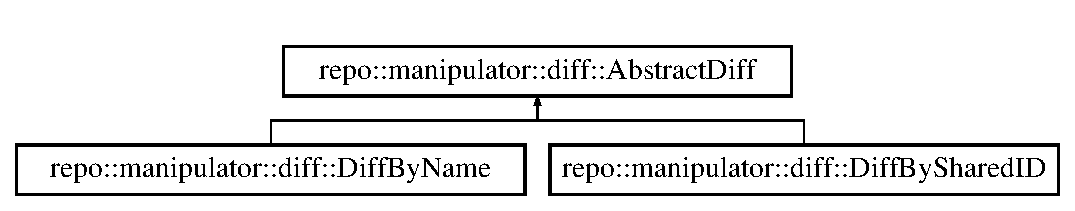
\includegraphics[height=2.000000cm]{classrepo_1_1manipulator_1_1diff_1_1_abstract_diff}
\end{center}
\end{figure}
\subsection*{Public Member Functions}
\begin{DoxyCompactItemize}
\item 
\hyperlink{classrepo_1_1manipulator_1_1diff_1_1_abstract_diff_a749b6fb18947b6bf78e6b1a59917ef86}{Abstract\+Diff} (const \hyperlink{classrepo_1_1core_1_1model_1_1_repo_scene}{repo\+::core\+::model\+::\+Repo\+Scene} $\ast$base, const \hyperlink{classrepo_1_1core_1_1model_1_1_repo_scene}{repo\+::core\+::model\+::\+Repo\+Scene} $\ast$compare, const \hyperlink{classrepo_1_1core_1_1model_1_1_repo_scene_aefcacd6eb4c7774ac1bfe3a6b223337c}{repo\+::core\+::model\+::\+Repo\+Scene\+::\+Graph\+Type} \&g\+Type)
\item 
\hyperlink{structrepo__diff__result__t}{repo\+\_\+diff\+\_\+result\+\_\+t} \hyperlink{classrepo_1_1manipulator_1_1diff_1_1_abstract_diff_aac1a749709ed41868bdcce6277a1039a}{getrepo\+\_\+diff\+\_\+result\+\_\+t\+For\+Base} ()
\item 
\hyperlink{structrepo__diff__result__t}{repo\+\_\+diff\+\_\+result\+\_\+t} \hyperlink{classrepo_1_1manipulator_1_1diff_1_1_abstract_diff_a1393fd4cade1766b43d2644990efbf14}{getrepo\+\_\+diff\+\_\+result\+\_\+t\+For\+Comp} ()
\item 
virtual bool \hyperlink{classrepo_1_1manipulator_1_1diff_1_1_abstract_diff_a0c1780f099a434120e65835bd1514ebf}{is\+Ok} (std\+::string \&msg) const =0
\end{DoxyCompactItemize}
\subsection*{Protected Attributes}
\begin{DoxyCompactItemize}
\item 
\hypertarget{classrepo_1_1manipulator_1_1diff_1_1_abstract_diff_a8802318cb00d911138bb22e7ca174d32}{}const \hyperlink{classrepo_1_1core_1_1model_1_1_repo_scene}{repo\+::core\+::model\+::\+Repo\+Scene} $\ast$ {\bfseries base\+Scene}\label{classrepo_1_1manipulator_1_1diff_1_1_abstract_diff_a8802318cb00d911138bb22e7ca174d32}

\item 
\hypertarget{classrepo_1_1manipulator_1_1diff_1_1_abstract_diff_a78910dd93c9a275198113faf6f2f99be}{}const \hyperlink{classrepo_1_1core_1_1model_1_1_repo_scene}{repo\+::core\+::model\+::\+Repo\+Scene} $\ast$ {\bfseries compare\+Scene}\label{classrepo_1_1manipulator_1_1diff_1_1_abstract_diff_a78910dd93c9a275198113faf6f2f99be}

\item 
\hypertarget{classrepo_1_1manipulator_1_1diff_1_1_abstract_diff_ac2d749de6ca04418cdaa8ea8f7f0b2c0}{}const \hyperlink{classrepo_1_1core_1_1model_1_1_repo_scene_aefcacd6eb4c7774ac1bfe3a6b223337c}{repo\+::core\+::model\+::\+Repo\+Scene\+::\+Graph\+Type} {\bfseries g\+Type}\label{classrepo_1_1manipulator_1_1diff_1_1_abstract_diff_ac2d749de6ca04418cdaa8ea8f7f0b2c0}

\item 
\hypertarget{classrepo_1_1manipulator_1_1diff_1_1_abstract_diff_aafc9a406ae0d81c3fa22ce360f6ae977}{}\hyperlink{structrepo__diff__result__t}{repo\+\_\+diff\+\_\+result\+\_\+t} {\bfseries base\+Res}\label{classrepo_1_1manipulator_1_1diff_1_1_abstract_diff_aafc9a406ae0d81c3fa22ce360f6ae977}

\item 
\hypertarget{classrepo_1_1manipulator_1_1diff_1_1_abstract_diff_a76f8b662a075357d1b2700fdff728764}{}\hyperlink{structrepo__diff__result__t}{repo\+\_\+diff\+\_\+result\+\_\+t} {\bfseries comp\+Res}\label{classrepo_1_1manipulator_1_1diff_1_1_abstract_diff_a76f8b662a075357d1b2700fdff728764}

\end{DoxyCompactItemize}


\subsection{Constructor \& Destructor Documentation}
\hypertarget{classrepo_1_1manipulator_1_1diff_1_1_abstract_diff_a749b6fb18947b6bf78e6b1a59917ef86}{}\index{repo\+::manipulator\+::diff\+::\+Abstract\+Diff@{repo\+::manipulator\+::diff\+::\+Abstract\+Diff}!Abstract\+Diff@{Abstract\+Diff}}
\index{Abstract\+Diff@{Abstract\+Diff}!repo\+::manipulator\+::diff\+::\+Abstract\+Diff@{repo\+::manipulator\+::diff\+::\+Abstract\+Diff}}
\subsubsection[{Abstract\+Diff}]{\setlength{\rightskip}{0pt plus 5cm}Abstract\+Diff\+::\+Abstract\+Diff (
\begin{DoxyParamCaption}
\item[{const {\bf repo\+::core\+::model\+::\+Repo\+Scene} $\ast$}]{base, }
\item[{const {\bf repo\+::core\+::model\+::\+Repo\+Scene} $\ast$}]{compare, }
\item[{const {\bf repo\+::core\+::model\+::\+Repo\+Scene\+::\+Graph\+Type} \&}]{g\+Type}
\end{DoxyParamCaption}
)}\label{classrepo_1_1manipulator_1_1diff_1_1_abstract_diff_a749b6fb18947b6bf78e6b1a59917ef86}
Construct a diff comparator given the 2 scenes supplied 
\begin{DoxyParams}{Parameters}
{\em base} & base scene to compare from \\
\hline
{\em compare} & scene to compare against \\
\hline
{\em g\+Type} & graph type to diff \\
\hline
\end{DoxyParams}


\subsection{Member Function Documentation}
\hypertarget{classrepo_1_1manipulator_1_1diff_1_1_abstract_diff_aac1a749709ed41868bdcce6277a1039a}{}\index{repo\+::manipulator\+::diff\+::\+Abstract\+Diff@{repo\+::manipulator\+::diff\+::\+Abstract\+Diff}!getrepo\+\_\+diff\+\_\+result\+\_\+t\+For\+Base@{getrepo\+\_\+diff\+\_\+result\+\_\+t\+For\+Base}}
\index{getrepo\+\_\+diff\+\_\+result\+\_\+t\+For\+Base@{getrepo\+\_\+diff\+\_\+result\+\_\+t\+For\+Base}!repo\+::manipulator\+::diff\+::\+Abstract\+Diff@{repo\+::manipulator\+::diff\+::\+Abstract\+Diff}}
\subsubsection[{getrepo\+\_\+diff\+\_\+result\+\_\+t\+For\+Base}]{\setlength{\rightskip}{0pt plus 5cm}{\bf repo\+\_\+diff\+\_\+result\+\_\+t} repo\+::manipulator\+::diff\+::\+Abstract\+Diff\+::getrepo\+\_\+diff\+\_\+result\+\_\+t\+For\+Base (
\begin{DoxyParamCaption}
{}
\end{DoxyParamCaption}
)\hspace{0.3cm}{\ttfamily [inline]}}\label{classrepo_1_1manipulator_1_1diff_1_1_abstract_diff_aac1a749709ed41868bdcce6277a1039a}
Obtain the diff result in the perspective of the base scene \begin{DoxyReturn}{Returns}
return the diff result for base scene 
\end{DoxyReturn}
\hypertarget{classrepo_1_1manipulator_1_1diff_1_1_abstract_diff_a1393fd4cade1766b43d2644990efbf14}{}\index{repo\+::manipulator\+::diff\+::\+Abstract\+Diff@{repo\+::manipulator\+::diff\+::\+Abstract\+Diff}!getrepo\+\_\+diff\+\_\+result\+\_\+t\+For\+Comp@{getrepo\+\_\+diff\+\_\+result\+\_\+t\+For\+Comp}}
\index{getrepo\+\_\+diff\+\_\+result\+\_\+t\+For\+Comp@{getrepo\+\_\+diff\+\_\+result\+\_\+t\+For\+Comp}!repo\+::manipulator\+::diff\+::\+Abstract\+Diff@{repo\+::manipulator\+::diff\+::\+Abstract\+Diff}}
\subsubsection[{getrepo\+\_\+diff\+\_\+result\+\_\+t\+For\+Comp}]{\setlength{\rightskip}{0pt plus 5cm}{\bf repo\+\_\+diff\+\_\+result\+\_\+t} repo\+::manipulator\+::diff\+::\+Abstract\+Diff\+::getrepo\+\_\+diff\+\_\+result\+\_\+t\+For\+Comp (
\begin{DoxyParamCaption}
{}
\end{DoxyParamCaption}
)\hspace{0.3cm}{\ttfamily [inline]}}\label{classrepo_1_1manipulator_1_1diff_1_1_abstract_diff_a1393fd4cade1766b43d2644990efbf14}
Obtain the diff result in the perspective of the compare scene \begin{DoxyReturn}{Returns}
return the diff result for compare scene 
\end{DoxyReturn}
\hypertarget{classrepo_1_1manipulator_1_1diff_1_1_abstract_diff_a0c1780f099a434120e65835bd1514ebf}{}\index{repo\+::manipulator\+::diff\+::\+Abstract\+Diff@{repo\+::manipulator\+::diff\+::\+Abstract\+Diff}!is\+Ok@{is\+Ok}}
\index{is\+Ok@{is\+Ok}!repo\+::manipulator\+::diff\+::\+Abstract\+Diff@{repo\+::manipulator\+::diff\+::\+Abstract\+Diff}}
\subsubsection[{is\+Ok}]{\setlength{\rightskip}{0pt plus 5cm}virtual bool repo\+::manipulator\+::diff\+::\+Abstract\+Diff\+::is\+Ok (
\begin{DoxyParamCaption}
\item[{std\+::string \&}]{msg}
\end{DoxyParamCaption}
) const\hspace{0.3cm}{\ttfamily [pure virtual]}}\label{classrepo_1_1manipulator_1_1diff_1_1_abstract_diff_a0c1780f099a434120e65835bd1514ebf}
Check if comparator functioned fine 
\begin{DoxyParams}{Parameters}
{\em msg} & error message should boolean returns false \\
\hline
\end{DoxyParams}
\begin{DoxyReturn}{Returns}
returns true if comparator operated successfully 
\end{DoxyReturn}


Implemented in \hyperlink{classrepo_1_1manipulator_1_1diff_1_1_diff_by_shared_i_d_afc3b71c3c85050b703c6ca3412c275e2}{repo\+::manipulator\+::diff\+::\+Diff\+By\+Shared\+I\+D}, and \hyperlink{classrepo_1_1manipulator_1_1diff_1_1_diff_by_name_a4cb80e41c9543f130903d83d43d78f98}{repo\+::manipulator\+::diff\+::\+Diff\+By\+Name}.



The documentation for this class was generated from the following files\+:\begin{DoxyCompactItemize}
\item 
C\+:/\+Users/\+Carmen/3\+D Repo/\+Repo/3drepobouncer/bouncer/src/repo/manipulator/diff/repo\+\_\+diff\+\_\+abstract.\+h\item 
C\+:/\+Users/\+Carmen/3\+D Repo/\+Repo/3drepobouncer/bouncer/src/repo/manipulator/diff/repo\+\_\+diff\+\_\+abstract.\+cpp\end{DoxyCompactItemize}

\hypertarget{classrepo_1_1core_1_1model_1_1_abstract_graph}{}\section{repo\+:\+:core\+:\+:model\+:\+:Abstract\+Graph Class Reference}
\label{classrepo_1_1core_1_1model_1_1_abstract_graph}\index{repo\+::core\+::model\+::\+Abstract\+Graph@{repo\+::core\+::model\+::\+Abstract\+Graph}}
Inheritance diagram for repo\+:\+:core\+:\+:model\+:\+:Abstract\+Graph\+:\begin{figure}[H]
\begin{center}
\leavevmode
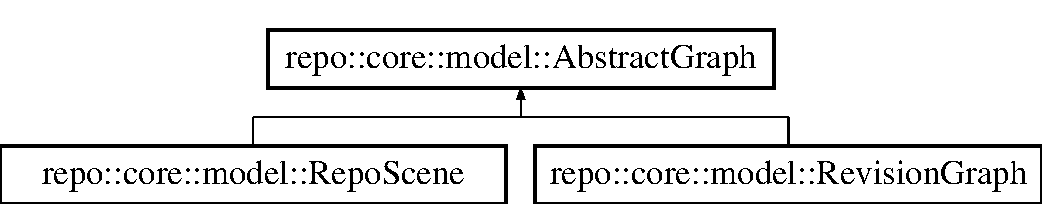
\includegraphics[height=2.000000cm]{classrepo_1_1core_1_1model_1_1_abstract_graph}
\end{center}
\end{figure}
\subsection*{Public Member Functions}
\begin{DoxyCompactItemize}
\item 
\hyperlink{classrepo_1_1core_1_1model_1_1_abstract_graph_ae2f85bcaf763abcaee115635b6e2af34}{Abstract\+Graph} (const std\+::string \&database\+Name=std\+::string(), const std\+::string \&\hyperlink{classrepo_1_1core_1_1model_1_1_abstract_graph_a8d6f646d8c8d0e5c14b31bbff17a1f1d}{project\+Name}=std\+::string())
\item 
virtual \hyperlink{classrepo_1_1core_1_1model_1_1_abstract_graph_a468a9dd5783926675495c2d5493fef32}{$\sim$\+Abstract\+Graph} ()
\end{DoxyCompactItemize}
\subsection*{Protected Attributes}
\begin{DoxyCompactItemize}
\item 
\hypertarget{classrepo_1_1core_1_1model_1_1_abstract_graph_a714110ab1bbe9bdf360fb475ccb60ef7}{}std\+::string {\bfseries database\+Name}\label{classrepo_1_1core_1_1model_1_1_abstract_graph_a714110ab1bbe9bdf360fb475ccb60ef7}

\item 
std\+::string \hyperlink{classrepo_1_1core_1_1model_1_1_abstract_graph_a8d6f646d8c8d0e5c14b31bbff17a1f1d}{project\+Name}
\end{DoxyCompactItemize}


\subsection{Constructor \& Destructor Documentation}
\hypertarget{classrepo_1_1core_1_1model_1_1_abstract_graph_ae2f85bcaf763abcaee115635b6e2af34}{}\index{repo\+::core\+::model\+::\+Abstract\+Graph@{repo\+::core\+::model\+::\+Abstract\+Graph}!Abstract\+Graph@{Abstract\+Graph}}
\index{Abstract\+Graph@{Abstract\+Graph}!repo\+::core\+::model\+::\+Abstract\+Graph@{repo\+::core\+::model\+::\+Abstract\+Graph}}
\subsubsection[{Abstract\+Graph}]{\setlength{\rightskip}{0pt plus 5cm}Abstract\+Graph\+::\+Abstract\+Graph (
\begin{DoxyParamCaption}
\item[{const std\+::string \&}]{database\+Name = {\ttfamily std\+:\+:string()}, }
\item[{const std\+::string \&}]{project\+Name = {\ttfamily std\+:\+:string()}}
\end{DoxyParamCaption}
)}\label{classrepo_1_1core_1_1model_1_1_abstract_graph_ae2f85bcaf763abcaee115635b6e2af34}
Constructor -\/ instantiates a new abstract graph with settings


\begin{DoxyParams}{Parameters}
{\em db\+Handler} & database handler (to read from/write to) \\
\hline
{\em database\+Name} & name of the database \\
\hline
{\em project\+Name} & name of the project \\
\hline
\end{DoxyParams}
\hypertarget{classrepo_1_1core_1_1model_1_1_abstract_graph_a468a9dd5783926675495c2d5493fef32}{}\index{repo\+::core\+::model\+::\+Abstract\+Graph@{repo\+::core\+::model\+::\+Abstract\+Graph}!````~Abstract\+Graph@{$\sim$\+Abstract\+Graph}}
\index{````~Abstract\+Graph@{$\sim$\+Abstract\+Graph}!repo\+::core\+::model\+::\+Abstract\+Graph@{repo\+::core\+::model\+::\+Abstract\+Graph}}
\subsubsection[{$\sim$\+Abstract\+Graph}]{\setlength{\rightskip}{0pt plus 5cm}Abstract\+Graph\+::$\sim$\+Abstract\+Graph (
\begin{DoxyParamCaption}
{}
\end{DoxyParamCaption}
)\hspace{0.3cm}{\ttfamily [virtual]}}\label{classrepo_1_1core_1_1model_1_1_abstract_graph_a468a9dd5783926675495c2d5493fef32}
Default Deconstructor 

\subsection{Member Data Documentation}
\hypertarget{classrepo_1_1core_1_1model_1_1_abstract_graph_a8d6f646d8c8d0e5c14b31bbff17a1f1d}{}\index{repo\+::core\+::model\+::\+Abstract\+Graph@{repo\+::core\+::model\+::\+Abstract\+Graph}!project\+Name@{project\+Name}}
\index{project\+Name@{project\+Name}!repo\+::core\+::model\+::\+Abstract\+Graph@{repo\+::core\+::model\+::\+Abstract\+Graph}}
\subsubsection[{project\+Name}]{\setlength{\rightskip}{0pt plus 5cm}std\+::string repo\+::core\+::model\+::\+Abstract\+Graph\+::project\+Name\hspace{0.3cm}{\ttfamily [protected]}}\label{classrepo_1_1core_1_1model_1_1_abstract_graph_a8d6f646d8c8d0e5c14b31bbff17a1f1d}
name of the database 

The documentation for this class was generated from the following files\+:\begin{DoxyCompactItemize}
\item 
C\+:/\+Users/\+Carmen/3\+D Repo/\+Repo/3drepobouncer/bouncer/src/repo/core/model/collection/repo\+\_\+graph\+\_\+abstract.\+h\item 
C\+:/\+Users/\+Carmen/3\+D Repo/\+Repo/3drepobouncer/bouncer/src/repo/core/model/collection/repo\+\_\+graph\+\_\+abstract.\+cpp\end{DoxyCompactItemize}

\hypertarget{classrepo_1_1manipulator_1_1modelconvertor_1_1_abstract_model_export}{}\section{repo\+:\+:manipulator\+:\+:modelconvertor\+:\+:Abstract\+Model\+Export Class Reference}
\label{classrepo_1_1manipulator_1_1modelconvertor_1_1_abstract_model_export}\index{repo\+::manipulator\+::modelconvertor\+::\+Abstract\+Model\+Export@{repo\+::manipulator\+::modelconvertor\+::\+Abstract\+Model\+Export}}
Inheritance diagram for repo\+:\+:manipulator\+:\+:modelconvertor\+:\+:Abstract\+Model\+Export\+:\begin{figure}[H]
\begin{center}
\leavevmode
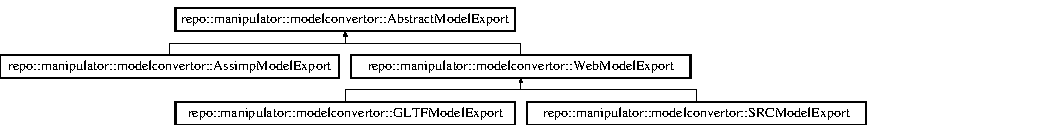
\includegraphics[height=1.671642cm]{classrepo_1_1manipulator_1_1modelconvertor_1_1_abstract_model_export}
\end{center}
\end{figure}
\subsection*{Public Member Functions}
\begin{DoxyCompactItemize}
\item 
\hyperlink{classrepo_1_1manipulator_1_1modelconvertor_1_1_abstract_model_export_a3e6a25bf60432759ce8be3837e46f309}{Abstract\+Model\+Export} (const \hyperlink{classrepo_1_1core_1_1model_1_1_repo_scene}{repo\+::core\+::model\+::\+Repo\+Scene} $\ast$scene)
\item 
virtual \hyperlink{classrepo_1_1manipulator_1_1modelconvertor_1_1_abstract_model_export_aecc655342a092127ed432a05da375291}{$\sim$\+Abstract\+Model\+Export} ()
\item 
virtual bool \hyperlink{classrepo_1_1manipulator_1_1modelconvertor_1_1_abstract_model_export_a305f2967d8112c5417b80fd3e8b8902a}{export\+To\+File} (const std\+::string \&file\+Path)=0
\end{DoxyCompactItemize}
\subsection*{Protected Attributes}
\begin{DoxyCompactItemize}
\item 
\hypertarget{classrepo_1_1manipulator_1_1modelconvertor_1_1_abstract_model_export_a7eb8d447b8a3a5687c682369dff23a70}{}const \hyperlink{classrepo_1_1core_1_1model_1_1_repo_scene}{repo\+::core\+::model\+::\+Repo\+Scene} $\ast$ {\bfseries scene}\label{classrepo_1_1manipulator_1_1modelconvertor_1_1_abstract_model_export_a7eb8d447b8a3a5687c682369dff23a70}

\end{DoxyCompactItemize}


\subsection{Constructor \& Destructor Documentation}
\hypertarget{classrepo_1_1manipulator_1_1modelconvertor_1_1_abstract_model_export_a3e6a25bf60432759ce8be3837e46f309}{}\index{repo\+::manipulator\+::modelconvertor\+::\+Abstract\+Model\+Export@{repo\+::manipulator\+::modelconvertor\+::\+Abstract\+Model\+Export}!Abstract\+Model\+Export@{Abstract\+Model\+Export}}
\index{Abstract\+Model\+Export@{Abstract\+Model\+Export}!repo\+::manipulator\+::modelconvertor\+::\+Abstract\+Model\+Export@{repo\+::manipulator\+::modelconvertor\+::\+Abstract\+Model\+Export}}
\subsubsection[{Abstract\+Model\+Export}]{\setlength{\rightskip}{0pt plus 5cm}Abstract\+Model\+Export\+::\+Abstract\+Model\+Export (
\begin{DoxyParamCaption}
\item[{const {\bf repo\+::core\+::model\+::\+Repo\+Scene} $\ast$}]{scene}
\end{DoxyParamCaption}
)}\label{classrepo_1_1manipulator_1_1modelconvertor_1_1_abstract_model_export_a3e6a25bf60432759ce8be3837e46f309}
Default Constructor, export model with default settings \hypertarget{classrepo_1_1manipulator_1_1modelconvertor_1_1_abstract_model_export_aecc655342a092127ed432a05da375291}{}\index{repo\+::manipulator\+::modelconvertor\+::\+Abstract\+Model\+Export@{repo\+::manipulator\+::modelconvertor\+::\+Abstract\+Model\+Export}!````~Abstract\+Model\+Export@{$\sim$\+Abstract\+Model\+Export}}
\index{````~Abstract\+Model\+Export@{$\sim$\+Abstract\+Model\+Export}!repo\+::manipulator\+::modelconvertor\+::\+Abstract\+Model\+Export@{repo\+::manipulator\+::modelconvertor\+::\+Abstract\+Model\+Export}}
\subsubsection[{$\sim$\+Abstract\+Model\+Export}]{\setlength{\rightskip}{0pt plus 5cm}Abstract\+Model\+Export\+::$\sim$\+Abstract\+Model\+Export (
\begin{DoxyParamCaption}
{}
\end{DoxyParamCaption}
)\hspace{0.3cm}{\ttfamily [virtual]}}\label{classrepo_1_1manipulator_1_1modelconvertor_1_1_abstract_model_export_aecc655342a092127ed432a05da375291}
Default Deconstructor 

\subsection{Member Function Documentation}
\hypertarget{classrepo_1_1manipulator_1_1modelconvertor_1_1_abstract_model_export_a305f2967d8112c5417b80fd3e8b8902a}{}\index{repo\+::manipulator\+::modelconvertor\+::\+Abstract\+Model\+Export@{repo\+::manipulator\+::modelconvertor\+::\+Abstract\+Model\+Export}!export\+To\+File@{export\+To\+File}}
\index{export\+To\+File@{export\+To\+File}!repo\+::manipulator\+::modelconvertor\+::\+Abstract\+Model\+Export@{repo\+::manipulator\+::modelconvertor\+::\+Abstract\+Model\+Export}}
\subsubsection[{export\+To\+File}]{\setlength{\rightskip}{0pt plus 5cm}virtual bool repo\+::manipulator\+::modelconvertor\+::\+Abstract\+Model\+Export\+::export\+To\+File (
\begin{DoxyParamCaption}
\item[{const std\+::string \&}]{file\+Path}
\end{DoxyParamCaption}
)\hspace{0.3cm}{\ttfamily [pure virtual]}}\label{classrepo_1_1manipulator_1_1modelconvertor_1_1_abstract_model_export_a305f2967d8112c5417b80fd3e8b8902a}
Export a repo scene graph to file 
\begin{DoxyParams}{Parameters}
{\em scene} & repo scene representation \\
\hline
{\em file\+Path} & path to destination file \\
\hline
\end{DoxyParams}
\begin{DoxyReturn}{Returns}
returns true upon success 
\end{DoxyReturn}


Implemented in \hyperlink{classrepo_1_1manipulator_1_1modelconvertor_1_1_assimp_model_export_afdf745f16a3d2f751ae236936111a875}{repo\+::manipulator\+::modelconvertor\+::\+Assimp\+Model\+Export}, and \hyperlink{classrepo_1_1manipulator_1_1modelconvertor_1_1_web_model_export_a7ce7f209d57bf5cd48499cf3dbbb25d0}{repo\+::manipulator\+::modelconvertor\+::\+Web\+Model\+Export}.



The documentation for this class was generated from the following files\+:\begin{DoxyCompactItemize}
\item 
C\+:/\+Users/\+Carmen/3\+D Repo/\+Repo/3drepobouncer/bouncer/src/repo/manipulator/modelconvertor/export/repo\+\_\+model\+\_\+export\+\_\+abstract.\+h\item 
C\+:/\+Users/\+Carmen/3\+D Repo/\+Repo/3drepobouncer/bouncer/src/repo/manipulator/modelconvertor/export/repo\+\_\+model\+\_\+export\+\_\+abstract.\+cpp\end{DoxyCompactItemize}

\hypertarget{classrepo_1_1manipulator_1_1modelconvertor_1_1_abstract_model_import}{}\section{repo\+:\+:manipulator\+:\+:modelconvertor\+:\+:Abstract\+Model\+Import Class Reference}
\label{classrepo_1_1manipulator_1_1modelconvertor_1_1_abstract_model_import}\index{repo\+::manipulator\+::modelconvertor\+::\+Abstract\+Model\+Import@{repo\+::manipulator\+::modelconvertor\+::\+Abstract\+Model\+Import}}
Inheritance diagram for repo\+:\+:manipulator\+:\+:modelconvertor\+:\+:Abstract\+Model\+Import\+:\begin{figure}[H]
\begin{center}
\leavevmode
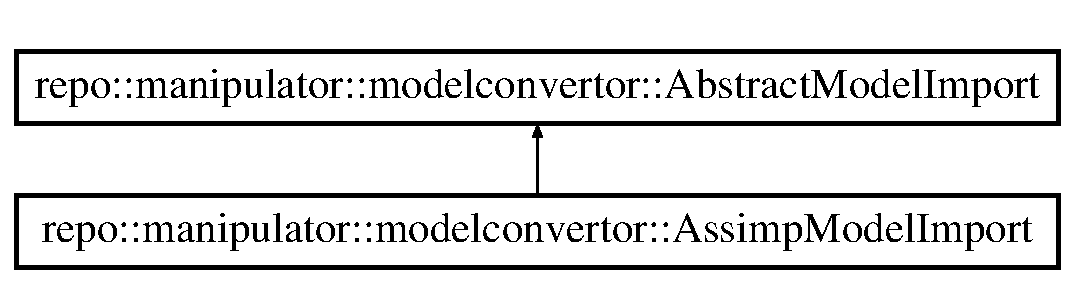
\includegraphics[height=2.000000cm]{classrepo_1_1manipulator_1_1modelconvertor_1_1_abstract_model_import}
\end{center}
\end{figure}
\subsection*{Public Member Functions}
\begin{DoxyCompactItemize}
\item 
\hyperlink{classrepo_1_1manipulator_1_1modelconvertor_1_1_abstract_model_import_a45ba12f9052b3cca1f1564bd5a05a8d8}{Abstract\+Model\+Import} ()
\item 
\hyperlink{classrepo_1_1manipulator_1_1modelconvertor_1_1_abstract_model_import_aed08f039d5132cde96f8c651f33b7877}{Abstract\+Model\+Import} (const \hyperlink{classrepo_1_1manipulator_1_1modelconvertor_1_1_model_import_config}{Model\+Import\+Config} $\ast$settings)
\item 
virtual \hyperlink{classrepo_1_1manipulator_1_1modelconvertor_1_1_abstract_model_import_a264ed6f9684aa0cf2216743e9f3c47cc}{$\sim$\+Abstract\+Model\+Import} ()
\item 
virtual \hyperlink{classrepo_1_1core_1_1model_1_1_repo_scene}{repo\+::core\+::model\+::\+Repo\+Scene} $\ast$ \hyperlink{classrepo_1_1manipulator_1_1modelconvertor_1_1_abstract_model_import_a0a0761d0a92ca05542b569a079f99c8f}{generate\+Repo\+Scene} ()=0
\item 
virtual bool \hyperlink{classrepo_1_1manipulator_1_1modelconvertor_1_1_abstract_model_import_a2b6296ea483d39f7ce6fe1e8a78124fd}{import\+Model} (std\+::string file\+Path, std\+::string \&err\+Msg)=0
\end{DoxyCompactItemize}
\subsection*{Protected Member Functions}
\begin{DoxyCompactItemize}
\item 
std\+::string \hyperlink{classrepo_1_1manipulator_1_1modelconvertor_1_1_abstract_model_import_a60b7f33101fe224ed25bd6b5d3f28ed5}{get\+Dir\+Path} (std\+::string full\+Path)
\item 
std\+::string \hyperlink{classrepo_1_1manipulator_1_1modelconvertor_1_1_abstract_model_import_adc928030621a646bee974229e741d43c}{get\+File\+Name} (std\+::string full\+Path)
\end{DoxyCompactItemize}
\subsection*{Protected Attributes}
\begin{DoxyCompactItemize}
\item 
\hypertarget{classrepo_1_1manipulator_1_1modelconvertor_1_1_abstract_model_import_ac32521c869840f34fbba44484d1d8ba5}{}const \hyperlink{classrepo_1_1manipulator_1_1modelconvertor_1_1_model_import_config}{Model\+Import\+Config} $\ast$ {\bfseries settings}\label{classrepo_1_1manipulator_1_1modelconvertor_1_1_abstract_model_import_ac32521c869840f34fbba44484d1d8ba5}

\item 
bool \hyperlink{classrepo_1_1manipulator_1_1modelconvertor_1_1_abstract_model_import_a9fd7153ec1348d4836f542f5bd51bfa5}{destroy\+Settings}
\end{DoxyCompactItemize}


\subsection{Constructor \& Destructor Documentation}
\hypertarget{classrepo_1_1manipulator_1_1modelconvertor_1_1_abstract_model_import_a45ba12f9052b3cca1f1564bd5a05a8d8}{}\index{repo\+::manipulator\+::modelconvertor\+::\+Abstract\+Model\+Import@{repo\+::manipulator\+::modelconvertor\+::\+Abstract\+Model\+Import}!Abstract\+Model\+Import@{Abstract\+Model\+Import}}
\index{Abstract\+Model\+Import@{Abstract\+Model\+Import}!repo\+::manipulator\+::modelconvertor\+::\+Abstract\+Model\+Import@{repo\+::manipulator\+::modelconvertor\+::\+Abstract\+Model\+Import}}
\subsubsection[{Abstract\+Model\+Import}]{\setlength{\rightskip}{0pt plus 5cm}Abstract\+Model\+Import\+::\+Abstract\+Model\+Import (
\begin{DoxyParamCaption}
{}
\end{DoxyParamCaption}
)}\label{classrepo_1_1manipulator_1_1modelconvertor_1_1_abstract_model_import_a45ba12f9052b3cca1f1564bd5a05a8d8}
Default Constructor, generate model with default settings \hypertarget{classrepo_1_1manipulator_1_1modelconvertor_1_1_abstract_model_import_aed08f039d5132cde96f8c651f33b7877}{}\index{repo\+::manipulator\+::modelconvertor\+::\+Abstract\+Model\+Import@{repo\+::manipulator\+::modelconvertor\+::\+Abstract\+Model\+Import}!Abstract\+Model\+Import@{Abstract\+Model\+Import}}
\index{Abstract\+Model\+Import@{Abstract\+Model\+Import}!repo\+::manipulator\+::modelconvertor\+::\+Abstract\+Model\+Import@{repo\+::manipulator\+::modelconvertor\+::\+Abstract\+Model\+Import}}
\subsubsection[{Abstract\+Model\+Import}]{\setlength{\rightskip}{0pt plus 5cm}Abstract\+Model\+Import\+::\+Abstract\+Model\+Import (
\begin{DoxyParamCaption}
\item[{const {\bf Model\+Import\+Config} $\ast$}]{settings}
\end{DoxyParamCaption}
)}\label{classrepo_1_1manipulator_1_1modelconvertor_1_1_abstract_model_import_aed08f039d5132cde96f8c651f33b7877}
Create \hyperlink{classrepo_1_1manipulator_1_1modelconvertor_1_1_abstract_model_import}{Abstract\+Model\+Import} with specific settings N\+O\+T\+E\+: The destructor will destroy the settings object referenced in this object! 
\begin{DoxyParams}{Parameters}
{\em settings} & \\
\hline
\end{DoxyParams}
\hypertarget{classrepo_1_1manipulator_1_1modelconvertor_1_1_abstract_model_import_a264ed6f9684aa0cf2216743e9f3c47cc}{}\index{repo\+::manipulator\+::modelconvertor\+::\+Abstract\+Model\+Import@{repo\+::manipulator\+::modelconvertor\+::\+Abstract\+Model\+Import}!````~Abstract\+Model\+Import@{$\sim$\+Abstract\+Model\+Import}}
\index{````~Abstract\+Model\+Import@{$\sim$\+Abstract\+Model\+Import}!repo\+::manipulator\+::modelconvertor\+::\+Abstract\+Model\+Import@{repo\+::manipulator\+::modelconvertor\+::\+Abstract\+Model\+Import}}
\subsubsection[{$\sim$\+Abstract\+Model\+Import}]{\setlength{\rightskip}{0pt plus 5cm}Abstract\+Model\+Import\+::$\sim$\+Abstract\+Model\+Import (
\begin{DoxyParamCaption}
{}
\end{DoxyParamCaption}
)\hspace{0.3cm}{\ttfamily [virtual]}}\label{classrepo_1_1manipulator_1_1modelconvertor_1_1_abstract_model_import_a264ed6f9684aa0cf2216743e9f3c47cc}
Default Deconstructor N\+O\+T\+E\+: The destructor will destroy the settings object referenced in this object! 

\subsection{Member Function Documentation}
\hypertarget{classrepo_1_1manipulator_1_1modelconvertor_1_1_abstract_model_import_a0a0761d0a92ca05542b569a079f99c8f}{}\index{repo\+::manipulator\+::modelconvertor\+::\+Abstract\+Model\+Import@{repo\+::manipulator\+::modelconvertor\+::\+Abstract\+Model\+Import}!generate\+Repo\+Scene@{generate\+Repo\+Scene}}
\index{generate\+Repo\+Scene@{generate\+Repo\+Scene}!repo\+::manipulator\+::modelconvertor\+::\+Abstract\+Model\+Import@{repo\+::manipulator\+::modelconvertor\+::\+Abstract\+Model\+Import}}
\subsubsection[{generate\+Repo\+Scene}]{\setlength{\rightskip}{0pt plus 5cm}virtual {\bf repo\+::core\+::model\+::\+Repo\+Scene}$\ast$ repo\+::manipulator\+::modelconvertor\+::\+Abstract\+Model\+Import\+::generate\+Repo\+Scene (
\begin{DoxyParamCaption}
{}
\end{DoxyParamCaption}
)\hspace{0.3cm}{\ttfamily [pure virtual]}}\label{classrepo_1_1manipulator_1_1modelconvertor_1_1_abstract_model_import_a0a0761d0a92ca05542b569a079f99c8f}
Generates a repo scene graph an internal representation needs to have been created before this call (e.\+g. by means of \hyperlink{classrepo_1_1manipulator_1_1modelconvertor_1_1_abstract_model_import_a2b6296ea483d39f7ce6fe1e8a78124fd}{import\+Model()}) \begin{DoxyReturn}{Returns}
returns a populated Repo\+Scene upon success. 
\end{DoxyReturn}


Implemented in \hyperlink{classrepo_1_1manipulator_1_1modelconvertor_1_1_assimp_model_import_a5e51038056aee890d4860190ce8d5847}{repo\+::manipulator\+::modelconvertor\+::\+Assimp\+Model\+Import}.

\hypertarget{classrepo_1_1manipulator_1_1modelconvertor_1_1_abstract_model_import_a60b7f33101fe224ed25bd6b5d3f28ed5}{}\index{repo\+::manipulator\+::modelconvertor\+::\+Abstract\+Model\+Import@{repo\+::manipulator\+::modelconvertor\+::\+Abstract\+Model\+Import}!get\+Dir\+Path@{get\+Dir\+Path}}
\index{get\+Dir\+Path@{get\+Dir\+Path}!repo\+::manipulator\+::modelconvertor\+::\+Abstract\+Model\+Import@{repo\+::manipulator\+::modelconvertor\+::\+Abstract\+Model\+Import}}
\subsubsection[{get\+Dir\+Path}]{\setlength{\rightskip}{0pt plus 5cm}std\+::string Abstract\+Model\+Import\+::get\+Dir\+Path (
\begin{DoxyParamCaption}
\item[{std\+::string}]{full\+Path}
\end{DoxyParamCaption}
)\hspace{0.3cm}{\ttfamily [protected]}}\label{classrepo_1_1manipulator_1_1modelconvertor_1_1_abstract_model_import_a60b7f33101fe224ed25bd6b5d3f28ed5}
Retrieve the directory to the file e.\+g /home/user/file.txt would return /home/user 
\begin{DoxyParams}{Parameters}
{\em full} & path of the file \\
\hline
\end{DoxyParams}
\begin{DoxyReturn}{Returns}
returns the path of the directory 
\end{DoxyReturn}
\hypertarget{classrepo_1_1manipulator_1_1modelconvertor_1_1_abstract_model_import_adc928030621a646bee974229e741d43c}{}\index{repo\+::manipulator\+::modelconvertor\+::\+Abstract\+Model\+Import@{repo\+::manipulator\+::modelconvertor\+::\+Abstract\+Model\+Import}!get\+File\+Name@{get\+File\+Name}}
\index{get\+File\+Name@{get\+File\+Name}!repo\+::manipulator\+::modelconvertor\+::\+Abstract\+Model\+Import@{repo\+::manipulator\+::modelconvertor\+::\+Abstract\+Model\+Import}}
\subsubsection[{get\+File\+Name}]{\setlength{\rightskip}{0pt plus 5cm}std\+::string Abstract\+Model\+Import\+::get\+File\+Name (
\begin{DoxyParamCaption}
\item[{std\+::string}]{full\+Path}
\end{DoxyParamCaption}
)\hspace{0.3cm}{\ttfamily [protected]}}\label{classrepo_1_1manipulator_1_1modelconvertor_1_1_abstract_model_import_adc928030621a646bee974229e741d43c}
Retrieve the filename from a full path e.\+g /home/user/file.txt would return file.\+txt 
\begin{DoxyParams}{Parameters}
{\em full} & path of the file \\
\hline
\end{DoxyParams}
\begin{DoxyReturn}{Returns}
returns the file name 
\end{DoxyReturn}
\hypertarget{classrepo_1_1manipulator_1_1modelconvertor_1_1_abstract_model_import_a2b6296ea483d39f7ce6fe1e8a78124fd}{}\index{repo\+::manipulator\+::modelconvertor\+::\+Abstract\+Model\+Import@{repo\+::manipulator\+::modelconvertor\+::\+Abstract\+Model\+Import}!import\+Model@{import\+Model}}
\index{import\+Model@{import\+Model}!repo\+::manipulator\+::modelconvertor\+::\+Abstract\+Model\+Import@{repo\+::manipulator\+::modelconvertor\+::\+Abstract\+Model\+Import}}
\subsubsection[{import\+Model}]{\setlength{\rightskip}{0pt plus 5cm}virtual bool repo\+::manipulator\+::modelconvertor\+::\+Abstract\+Model\+Import\+::import\+Model (
\begin{DoxyParamCaption}
\item[{std\+::string}]{file\+Path, }
\item[{std\+::string \&}]{err\+Msg}
\end{DoxyParamCaption}
)\hspace{0.3cm}{\ttfamily [pure virtual]}}\label{classrepo_1_1manipulator_1_1modelconvertor_1_1_abstract_model_import_a2b6296ea483d39f7ce6fe1e8a78124fd}
Import model from a given file This does not generate the Repo Scene Graph Use get\+Repo\+Scene() to generate a Repo Scene Graph. 
\begin{DoxyParams}{Parameters}
{\em path} & to the file \\
\hline
{\em error} & message if failed \\
\hline
\end{DoxyParams}
\begin{DoxyReturn}{Returns}
returns true upon success 
\end{DoxyReturn}


Implemented in \hyperlink{classrepo_1_1manipulator_1_1modelconvertor_1_1_assimp_model_import_aefdfec79f7be00e1ad452ee22555b64a}{repo\+::manipulator\+::modelconvertor\+::\+Assimp\+Model\+Import}.



\subsection{Member Data Documentation}
\hypertarget{classrepo_1_1manipulator_1_1modelconvertor_1_1_abstract_model_import_a9fd7153ec1348d4836f542f5bd51bfa5}{}\index{repo\+::manipulator\+::modelconvertor\+::\+Abstract\+Model\+Import@{repo\+::manipulator\+::modelconvertor\+::\+Abstract\+Model\+Import}!destroy\+Settings@{destroy\+Settings}}
\index{destroy\+Settings@{destroy\+Settings}!repo\+::manipulator\+::modelconvertor\+::\+Abstract\+Model\+Import@{repo\+::manipulator\+::modelconvertor\+::\+Abstract\+Model\+Import}}
\subsubsection[{destroy\+Settings}]{\setlength{\rightskip}{0pt plus 5cm}bool repo\+::manipulator\+::modelconvertor\+::\+Abstract\+Model\+Import\+::destroy\+Settings\hspace{0.3cm}{\ttfamily [protected]}}\label{classrepo_1_1manipulator_1_1modelconvertor_1_1_abstract_model_import_a9fd7153ec1348d4836f542f5bd51bfa5}
Stores related settings for model import 

The documentation for this class was generated from the following files\+:\begin{DoxyCompactItemize}
\item 
C\+:/\+Users/\+Carmen/3\+D Repo/\+Repo/3drepobouncer/bouncer/src/repo/manipulator/modelconvertor/import/repo\+\_\+model\+\_\+import\+\_\+abstract.\+h\item 
C\+:/\+Users/\+Carmen/3\+D Repo/\+Repo/3drepobouncer/bouncer/src/repo/manipulator/modelconvertor/import/repo\+\_\+model\+\_\+import\+\_\+abstract.\+cpp\end{DoxyCompactItemize}

\hypertarget{classrepo_1_1manipulator_1_1modeloptimizer_1_1_abstract_optimizer}{}\section{repo\+:\+:manipulator\+:\+:modeloptimizer\+:\+:Abstract\+Optimizer Class Reference}
\label{classrepo_1_1manipulator_1_1modeloptimizer_1_1_abstract_optimizer}\index{repo\+::manipulator\+::modeloptimizer\+::\+Abstract\+Optimizer@{repo\+::manipulator\+::modeloptimizer\+::\+Abstract\+Optimizer}}
Inheritance diagram for repo\+:\+:manipulator\+:\+:modeloptimizer\+:\+:Abstract\+Optimizer\+:\begin{figure}[H]
\begin{center}
\leavevmode
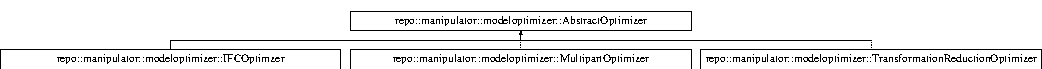
\includegraphics[height=0.921811cm]{classrepo_1_1manipulator_1_1modeloptimizer_1_1_abstract_optimizer}
\end{center}
\end{figure}
\subsection*{Public Member Functions}
\begin{DoxyCompactItemize}
\item 
\hyperlink{classrepo_1_1manipulator_1_1modeloptimizer_1_1_abstract_optimizer_a9a592c40d89082c63a4e602fed426469}{Abstract\+Optimizer} ()
\item 
virtual \hyperlink{classrepo_1_1manipulator_1_1modeloptimizer_1_1_abstract_optimizer_ab86ed975e5691c531e5ef528379ec60b}{$\sim$\+Abstract\+Optimizer} ()
\item 
virtual bool \hyperlink{classrepo_1_1manipulator_1_1modeloptimizer_1_1_abstract_optimizer_a38e98344c1d3c66fbea8adae41dc6cb1}{apply} (\hyperlink{classrepo_1_1core_1_1model_1_1_repo_scene}{repo\+::core\+::model\+::\+Repo\+Scene} $\ast$scene)=0
\end{DoxyCompactItemize}


\subsection{Constructor \& Destructor Documentation}
\hypertarget{classrepo_1_1manipulator_1_1modeloptimizer_1_1_abstract_optimizer_a9a592c40d89082c63a4e602fed426469}{}\index{repo\+::manipulator\+::modeloptimizer\+::\+Abstract\+Optimizer@{repo\+::manipulator\+::modeloptimizer\+::\+Abstract\+Optimizer}!Abstract\+Optimizer@{Abstract\+Optimizer}}
\index{Abstract\+Optimizer@{Abstract\+Optimizer}!repo\+::manipulator\+::modeloptimizer\+::\+Abstract\+Optimizer@{repo\+::manipulator\+::modeloptimizer\+::\+Abstract\+Optimizer}}
\subsubsection[{Abstract\+Optimizer}]{\setlength{\rightskip}{0pt plus 5cm}Abstract\+Optimizer\+::\+Abstract\+Optimizer (
\begin{DoxyParamCaption}
{}
\end{DoxyParamCaption}
)}\label{classrepo_1_1manipulator_1_1modeloptimizer_1_1_abstract_optimizer_a9a592c40d89082c63a4e602fed426469}
Default constructor \hypertarget{classrepo_1_1manipulator_1_1modeloptimizer_1_1_abstract_optimizer_ab86ed975e5691c531e5ef528379ec60b}{}\index{repo\+::manipulator\+::modeloptimizer\+::\+Abstract\+Optimizer@{repo\+::manipulator\+::modeloptimizer\+::\+Abstract\+Optimizer}!````~Abstract\+Optimizer@{$\sim$\+Abstract\+Optimizer}}
\index{````~Abstract\+Optimizer@{$\sim$\+Abstract\+Optimizer}!repo\+::manipulator\+::modeloptimizer\+::\+Abstract\+Optimizer@{repo\+::manipulator\+::modeloptimizer\+::\+Abstract\+Optimizer}}
\subsubsection[{$\sim$\+Abstract\+Optimizer}]{\setlength{\rightskip}{0pt plus 5cm}Abstract\+Optimizer\+::$\sim$\+Abstract\+Optimizer (
\begin{DoxyParamCaption}
{}
\end{DoxyParamCaption}
)\hspace{0.3cm}{\ttfamily [virtual]}}\label{classrepo_1_1manipulator_1_1modeloptimizer_1_1_abstract_optimizer_ab86ed975e5691c531e5ef528379ec60b}
Default deconstructor 

\subsection{Member Function Documentation}
\hypertarget{classrepo_1_1manipulator_1_1modeloptimizer_1_1_abstract_optimizer_a38e98344c1d3c66fbea8adae41dc6cb1}{}\index{repo\+::manipulator\+::modeloptimizer\+::\+Abstract\+Optimizer@{repo\+::manipulator\+::modeloptimizer\+::\+Abstract\+Optimizer}!apply@{apply}}
\index{apply@{apply}!repo\+::manipulator\+::modeloptimizer\+::\+Abstract\+Optimizer@{repo\+::manipulator\+::modeloptimizer\+::\+Abstract\+Optimizer}}
\subsubsection[{apply}]{\setlength{\rightskip}{0pt plus 5cm}virtual bool repo\+::manipulator\+::modeloptimizer\+::\+Abstract\+Optimizer\+::apply (
\begin{DoxyParamCaption}
\item[{{\bf repo\+::core\+::model\+::\+Repo\+Scene} $\ast$}]{scene}
\end{DoxyParamCaption}
)\hspace{0.3cm}{\ttfamily [pure virtual]}}\label{classrepo_1_1manipulator_1_1modeloptimizer_1_1_abstract_optimizer_a38e98344c1d3c66fbea8adae41dc6cb1}
Apply optimisation on the given repo\+Scene 
\begin{DoxyParams}{Parameters}
{\em scene} & takes in a repo\+Scene to optimise \\
\hline
\end{DoxyParams}
\begin{DoxyReturn}{Returns}
returns true upon success 
\end{DoxyReturn}


Implemented in \hyperlink{classrepo_1_1manipulator_1_1modeloptimizer_1_1_transformation_reduction_optimizer_ab1e06e1810e27b99030cf1d86c1b4e06}{repo\+::manipulator\+::modeloptimizer\+::\+Transformation\+Reduction\+Optimizer}, \hyperlink{classrepo_1_1manipulator_1_1modeloptimizer_1_1_multipart_optimizer_a3e223c461f5b27c09f9037a57ff3fd01}{repo\+::manipulator\+::modeloptimizer\+::\+Multipart\+Optimizer}, and \hyperlink{classrepo_1_1manipulator_1_1modeloptimizer_1_1_i_f_c_optimzer_a5ea4e1e6cd502d72a3ba3cca593eb9d3}{repo\+::manipulator\+::modeloptimizer\+::\+I\+F\+C\+Optimzer}.



The documentation for this class was generated from the following files\+:\begin{DoxyCompactItemize}
\item 
C\+:/\+Users/\+Carmen/3\+D Repo/\+Repo/3drepobouncer/bouncer/src/repo/manipulator/modeloptimizer/repo\+\_\+optimizer\+\_\+abstract.\+h\item 
C\+:/\+Users/\+Carmen/3\+D Repo/\+Repo/3drepobouncer/bouncer/src/repo/manipulator/modeloptimizer/repo\+\_\+optimizer\+\_\+abstract.\+cpp\end{DoxyCompactItemize}

\hypertarget{classrepo_1_1manipulator_1_1modelutility_1_1_abstract_spatial_partitioner}{}\section{repo\+:\+:manipulator\+:\+:modelutility\+:\+:Abstract\+Spatial\+Partitioner Class Reference}
\label{classrepo_1_1manipulator_1_1modelutility_1_1_abstract_spatial_partitioner}\index{repo\+::manipulator\+::modelutility\+::\+Abstract\+Spatial\+Partitioner@{repo\+::manipulator\+::modelutility\+::\+Abstract\+Spatial\+Partitioner}}
Inheritance diagram for repo\+:\+:manipulator\+:\+:modelutility\+:\+:Abstract\+Spatial\+Partitioner\+:\begin{figure}[H]
\begin{center}
\leavevmode
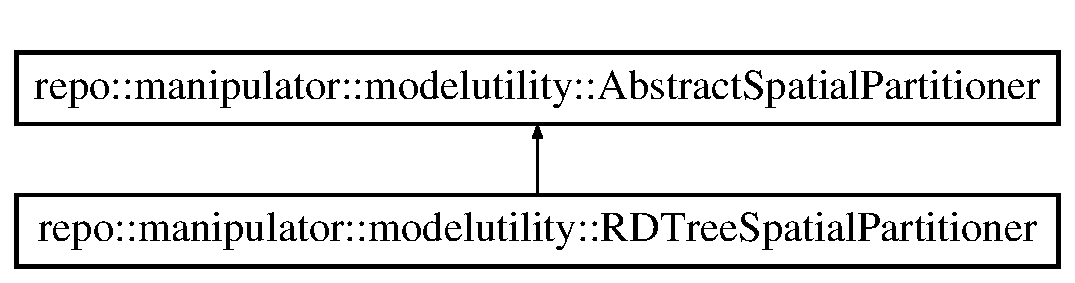
\includegraphics[height=2.000000cm]{classrepo_1_1manipulator_1_1modelutility_1_1_abstract_spatial_partitioner}
\end{center}
\end{figure}
\subsection*{Public Member Functions}
\begin{DoxyCompactItemize}
\item 
\hyperlink{classrepo_1_1manipulator_1_1modelutility_1_1_abstract_spatial_partitioner_a9fb21ce83e682d89be17768c7b02cdf3}{Abstract\+Spatial\+Partitioner} (const \hyperlink{classrepo_1_1core_1_1model_1_1_repo_scene}{repo\+::core\+::model\+::\+Repo\+Scene} $\ast$scene, const uint32\+\_\+t \&max\+Depth)
\item 
virtual std\+::shared\+\_\+ptr$<$ \hyperlink{structrepo__partitioning__tree__t}{repo\+\_\+partitioning\+\_\+tree\+\_\+t} $>$ \hyperlink{classrepo_1_1manipulator_1_1modelutility_1_1_abstract_spatial_partitioner_af1e6e3540698ff0f4ec52cd758260aba}{partition\+Scene} ()=0
\item 
virtual \hyperlink{classrepo_1_1lib_1_1_property_tree}{repo\+::lib\+::\+Property\+Tree} \hyperlink{classrepo_1_1manipulator_1_1modelutility_1_1_abstract_spatial_partitioner_a46d182fa325b972a66b65009975e5980}{generate\+Property\+Tree\+For\+Partitioning} ()
\end{DoxyCompactItemize}
\subsection*{Protected Member Functions}
\begin{DoxyCompactItemize}
\item 
\hypertarget{classrepo_1_1manipulator_1_1modelutility_1_1_abstract_spatial_partitioner_a712a25e95b83e7de662e2e92b9c931c2}{}\hyperlink{classrepo_1_1lib_1_1_property_tree}{repo\+::lib\+::\+Property\+Tree} {\bfseries generate\+Property\+Tree\+For\+Partitioning\+Internal} (const std\+::shared\+\_\+ptr$<$ \hyperlink{structrepo__partitioning__tree__t}{repo\+\_\+partitioning\+\_\+tree\+\_\+t} $>$ \&sp\+Tree) const \label{classrepo_1_1manipulator_1_1modelutility_1_1_abstract_spatial_partitioner_a712a25e95b83e7de662e2e92b9c931c2}

\end{DoxyCompactItemize}
\subsection*{Protected Attributes}
\begin{DoxyCompactItemize}
\item 
\hypertarget{classrepo_1_1manipulator_1_1modelutility_1_1_abstract_spatial_partitioner_acc5184e4cdcbded21d68bdfb661ce4c4}{}const \hyperlink{classrepo_1_1core_1_1model_1_1_repo_scene}{repo\+::core\+::model\+::\+Repo\+Scene} $\ast$ {\bfseries scene}\label{classrepo_1_1manipulator_1_1modelutility_1_1_abstract_spatial_partitioner_acc5184e4cdcbded21d68bdfb661ce4c4}

\item 
\hypertarget{classrepo_1_1manipulator_1_1modelutility_1_1_abstract_spatial_partitioner_a8f3d011aeb4f2b8c546cf8c470ac362e}{}const uint32\+\_\+t {\bfseries max\+Depth}\label{classrepo_1_1manipulator_1_1modelutility_1_1_abstract_spatial_partitioner_a8f3d011aeb4f2b8c546cf8c470ac362e}

\item 
\hypertarget{classrepo_1_1manipulator_1_1modelutility_1_1_abstract_spatial_partitioner_abc8b608e271174e8cb1ef539a2dfe80d}{}const \hyperlink{classrepo_1_1core_1_1model_1_1_repo_scene_aefcacd6eb4c7774ac1bfe3a6b223337c}{repo\+::core\+::model\+::\+Repo\+Scene\+::\+Graph\+Type} {\bfseries g\+Type}\label{classrepo_1_1manipulator_1_1modelutility_1_1_abstract_spatial_partitioner_abc8b608e271174e8cb1ef539a2dfe80d}

\end{DoxyCompactItemize}


\subsection{Constructor \& Destructor Documentation}
\hypertarget{classrepo_1_1manipulator_1_1modelutility_1_1_abstract_spatial_partitioner_a9fb21ce83e682d89be17768c7b02cdf3}{}\index{repo\+::manipulator\+::modelutility\+::\+Abstract\+Spatial\+Partitioner@{repo\+::manipulator\+::modelutility\+::\+Abstract\+Spatial\+Partitioner}!Abstract\+Spatial\+Partitioner@{Abstract\+Spatial\+Partitioner}}
\index{Abstract\+Spatial\+Partitioner@{Abstract\+Spatial\+Partitioner}!repo\+::manipulator\+::modelutility\+::\+Abstract\+Spatial\+Partitioner@{repo\+::manipulator\+::modelutility\+::\+Abstract\+Spatial\+Partitioner}}
\subsubsection[{Abstract\+Spatial\+Partitioner}]{\setlength{\rightskip}{0pt plus 5cm}Abstract\+Spatial\+Partitioner\+::\+Abstract\+Spatial\+Partitioner (
\begin{DoxyParamCaption}
\item[{const {\bf repo\+::core\+::model\+::\+Repo\+Scene} $\ast$}]{scene, }
\item[{const uint32\+\_\+t \&}]{max\+Depth}
\end{DoxyParamCaption}
)}\label{classrepo_1_1manipulator_1_1modelutility_1_1_abstract_spatial_partitioner_a9fb21ce83e682d89be17768c7b02cdf3}
Abstract Spatial Partitioning utility class to spatially divide a scene graph base on its meshes Note\+: currently only support scene with optimised graph! 
\begin{DoxyParams}{Parameters}
{\em scene} & scene to divide \\
\hline
{\em depth} & limiting depth of the tree \\
\hline
\end{DoxyParams}


\subsection{Member Function Documentation}
\hypertarget{classrepo_1_1manipulator_1_1modelutility_1_1_abstract_spatial_partitioner_a46d182fa325b972a66b65009975e5980}{}\index{repo\+::manipulator\+::modelutility\+::\+Abstract\+Spatial\+Partitioner@{repo\+::manipulator\+::modelutility\+::\+Abstract\+Spatial\+Partitioner}!generate\+Property\+Tree\+For\+Partitioning@{generate\+Property\+Tree\+For\+Partitioning}}
\index{generate\+Property\+Tree\+For\+Partitioning@{generate\+Property\+Tree\+For\+Partitioning}!repo\+::manipulator\+::modelutility\+::\+Abstract\+Spatial\+Partitioner@{repo\+::manipulator\+::modelutility\+::\+Abstract\+Spatial\+Partitioner}}
\subsubsection[{generate\+Property\+Tree\+For\+Partitioning}]{\setlength{\rightskip}{0pt plus 5cm}{\bf repo\+::lib\+::\+Property\+Tree} Abstract\+Spatial\+Partitioner\+::generate\+Property\+Tree\+For\+Partitioning (
\begin{DoxyParamCaption}
{}
\end{DoxyParamCaption}
)\hspace{0.3cm}{\ttfamily [virtual]}}\label{classrepo_1_1manipulator_1_1modelutility_1_1_abstract_spatial_partitioner_a46d182fa325b972a66b65009975e5980}
Generate a property tree representing the \hyperlink{structrepo__partitioning__tree__t}{repo\+\_\+partitioning\+\_\+tree\+\_\+t} from \hyperlink{classrepo_1_1manipulator_1_1modelutility_1_1_abstract_spatial_partitioner_af1e6e3540698ff0f4ec52cd758260aba}{partition\+Scene()} \begin{DoxyReturn}{Returns}
returns the spatial partitioning information as a property tree 
\end{DoxyReturn}
\hypertarget{classrepo_1_1manipulator_1_1modelutility_1_1_abstract_spatial_partitioner_af1e6e3540698ff0f4ec52cd758260aba}{}\index{repo\+::manipulator\+::modelutility\+::\+Abstract\+Spatial\+Partitioner@{repo\+::manipulator\+::modelutility\+::\+Abstract\+Spatial\+Partitioner}!partition\+Scene@{partition\+Scene}}
\index{partition\+Scene@{partition\+Scene}!repo\+::manipulator\+::modelutility\+::\+Abstract\+Spatial\+Partitioner@{repo\+::manipulator\+::modelutility\+::\+Abstract\+Spatial\+Partitioner}}
\subsubsection[{partition\+Scene}]{\setlength{\rightskip}{0pt plus 5cm}virtual std\+::shared\+\_\+ptr$<${\bf repo\+\_\+partitioning\+\_\+tree\+\_\+t}$>$ repo\+::manipulator\+::modelutility\+::\+Abstract\+Spatial\+Partitioner\+::partition\+Scene (
\begin{DoxyParamCaption}
{}
\end{DoxyParamCaption}
)\hspace{0.3cm}{\ttfamily [pure virtual]}}\label{classrepo_1_1manipulator_1_1modelutility_1_1_abstract_spatial_partitioner_af1e6e3540698ff0f4ec52cd758260aba}
Partition the scene \begin{DoxyReturn}{Returns}
returns the spatial partitioning information as a tree 
\end{DoxyReturn}


Implemented in \hyperlink{classrepo_1_1manipulator_1_1modelutility_1_1_r_d_tree_spatial_partitioner_a768852ef54d357e43b86a70897002623}{repo\+::manipulator\+::modelutility\+::\+R\+D\+Tree\+Spatial\+Partitioner}.



The documentation for this class was generated from the following files\+:\begin{DoxyCompactItemize}
\item 
C\+:/\+Users/\+Carmen/3\+D Repo/\+Repo/3drepobouncer/bouncer/src/repo/manipulator/modelutility/spatialpartitioning/repo\+\_\+spatial\+\_\+partitioner\+\_\+abstract.\+h\item 
C\+:/\+Users/\+Carmen/3\+D Repo/\+Repo/3drepobouncer/bouncer/src/repo/manipulator/modelutility/spatialpartitioning/repo\+\_\+spatial\+\_\+partitioner\+\_\+abstract.\+cpp\end{DoxyCompactItemize}

\hypertarget{classrepo_1_1manipulator_1_1modelconvertor_1_1_assimp_model_export}{}\section{repo\+:\+:manipulator\+:\+:modelconvertor\+:\+:Assimp\+Model\+Export Class Reference}
\label{classrepo_1_1manipulator_1_1modelconvertor_1_1_assimp_model_export}\index{repo\+::manipulator\+::modelconvertor\+::\+Assimp\+Model\+Export@{repo\+::manipulator\+::modelconvertor\+::\+Assimp\+Model\+Export}}
Inheritance diagram for repo\+:\+:manipulator\+:\+:modelconvertor\+:\+:Assimp\+Model\+Export\+:\begin{figure}[H]
\begin{center}
\leavevmode
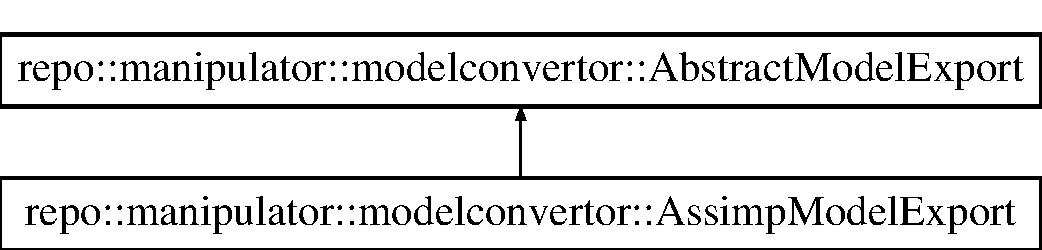
\includegraphics[height=2.000000cm]{classrepo_1_1manipulator_1_1modelconvertor_1_1_assimp_model_export}
\end{center}
\end{figure}
\subsection*{Public Member Functions}
\begin{DoxyCompactItemize}
\item 
\hyperlink{classrepo_1_1manipulator_1_1modelconvertor_1_1_assimp_model_export_a8971989a7e2b8d457f81a412ffb3bc0c}{Assimp\+Model\+Export} (const \hyperlink{classrepo_1_1core_1_1model_1_1_repo_scene}{repo\+::core\+::model\+::\+Repo\+Scene} $\ast$scene)
\item 
virtual \hyperlink{classrepo_1_1manipulator_1_1modelconvertor_1_1_assimp_model_export_a2ce15aaa7d4eae90f24354e16d5f7e5b}{$\sim$\+Assimp\+Model\+Export} ()
\item 
bool \hyperlink{classrepo_1_1manipulator_1_1modelconvertor_1_1_assimp_model_export_afdf745f16a3d2f751ae236936111a875}{export\+To\+File} (const std\+::string \&file\+Path)
\end{DoxyCompactItemize}
\subsection*{Static Public Member Functions}
\begin{DoxyCompactItemize}
\item 
static std\+::string \hyperlink{classrepo_1_1manipulator_1_1modelconvertor_1_1_assimp_model_export_ae36fc6ff94ca7e6c86dc5b0f7ee18fba}{get\+Supported\+Formats} ()
\end{DoxyCompactItemize}
\subsection*{Additional Inherited Members}


\subsection{Constructor \& Destructor Documentation}
\hypertarget{classrepo_1_1manipulator_1_1modelconvertor_1_1_assimp_model_export_a8971989a7e2b8d457f81a412ffb3bc0c}{}\index{repo\+::manipulator\+::modelconvertor\+::\+Assimp\+Model\+Export@{repo\+::manipulator\+::modelconvertor\+::\+Assimp\+Model\+Export}!Assimp\+Model\+Export@{Assimp\+Model\+Export}}
\index{Assimp\+Model\+Export@{Assimp\+Model\+Export}!repo\+::manipulator\+::modelconvertor\+::\+Assimp\+Model\+Export@{repo\+::manipulator\+::modelconvertor\+::\+Assimp\+Model\+Export}}
\subsubsection[{Assimp\+Model\+Export}]{\setlength{\rightskip}{0pt plus 5cm}Assimp\+Model\+Export\+::\+Assimp\+Model\+Export (
\begin{DoxyParamCaption}
\item[{const {\bf repo\+::core\+::model\+::\+Repo\+Scene} $\ast$}]{scene}
\end{DoxyParamCaption}
)}\label{classrepo_1_1manipulator_1_1modelconvertor_1_1_assimp_model_export_a8971989a7e2b8d457f81a412ffb3bc0c}
Default Constructor, export model with default settings \hypertarget{classrepo_1_1manipulator_1_1modelconvertor_1_1_assimp_model_export_a2ce15aaa7d4eae90f24354e16d5f7e5b}{}\index{repo\+::manipulator\+::modelconvertor\+::\+Assimp\+Model\+Export@{repo\+::manipulator\+::modelconvertor\+::\+Assimp\+Model\+Export}!````~Assimp\+Model\+Export@{$\sim$\+Assimp\+Model\+Export}}
\index{````~Assimp\+Model\+Export@{$\sim$\+Assimp\+Model\+Export}!repo\+::manipulator\+::modelconvertor\+::\+Assimp\+Model\+Export@{repo\+::manipulator\+::modelconvertor\+::\+Assimp\+Model\+Export}}
\subsubsection[{$\sim$\+Assimp\+Model\+Export}]{\setlength{\rightskip}{0pt plus 5cm}Assimp\+Model\+Export\+::$\sim$\+Assimp\+Model\+Export (
\begin{DoxyParamCaption}
{}
\end{DoxyParamCaption}
)\hspace{0.3cm}{\ttfamily [virtual]}}\label{classrepo_1_1manipulator_1_1modelconvertor_1_1_assimp_model_export_a2ce15aaa7d4eae90f24354e16d5f7e5b}
Default Deconstructor 

\subsection{Member Function Documentation}
\hypertarget{classrepo_1_1manipulator_1_1modelconvertor_1_1_assimp_model_export_afdf745f16a3d2f751ae236936111a875}{}\index{repo\+::manipulator\+::modelconvertor\+::\+Assimp\+Model\+Export@{repo\+::manipulator\+::modelconvertor\+::\+Assimp\+Model\+Export}!export\+To\+File@{export\+To\+File}}
\index{export\+To\+File@{export\+To\+File}!repo\+::manipulator\+::modelconvertor\+::\+Assimp\+Model\+Export@{repo\+::manipulator\+::modelconvertor\+::\+Assimp\+Model\+Export}}
\subsubsection[{export\+To\+File}]{\setlength{\rightskip}{0pt plus 5cm}bool Assimp\+Model\+Export\+::export\+To\+File (
\begin{DoxyParamCaption}
\item[{const std\+::string \&}]{file\+Path}
\end{DoxyParamCaption}
)\hspace{0.3cm}{\ttfamily [virtual]}}\label{classrepo_1_1manipulator_1_1modelconvertor_1_1_assimp_model_export_afdf745f16a3d2f751ae236936111a875}
Export a repo scene graph to file 
\begin{DoxyParams}{Parameters}
{\em scene} & repo scene representation \\
\hline
{\em file\+Path} & path to destination file \\
\hline
\end{DoxyParams}
\begin{DoxyReturn}{Returns}
returns true upon success 
\end{DoxyReturn}


Implements \hyperlink{classrepo_1_1manipulator_1_1modelconvertor_1_1_abstract_model_export_a305f2967d8112c5417b80fd3e8b8902a}{repo\+::manipulator\+::modelconvertor\+::\+Abstract\+Model\+Export}.

\hypertarget{classrepo_1_1manipulator_1_1modelconvertor_1_1_assimp_model_export_ae36fc6ff94ca7e6c86dc5b0f7ee18fba}{}\index{repo\+::manipulator\+::modelconvertor\+::\+Assimp\+Model\+Export@{repo\+::manipulator\+::modelconvertor\+::\+Assimp\+Model\+Export}!get\+Supported\+Formats@{get\+Supported\+Formats}}
\index{get\+Supported\+Formats@{get\+Supported\+Formats}!repo\+::manipulator\+::modelconvertor\+::\+Assimp\+Model\+Export@{repo\+::manipulator\+::modelconvertor\+::\+Assimp\+Model\+Export}}
\subsubsection[{get\+Supported\+Formats}]{\setlength{\rightskip}{0pt plus 5cm}std\+::string Assimp\+Model\+Export\+::get\+Supported\+Formats (
\begin{DoxyParamCaption}
{}
\end{DoxyParamCaption}
)\hspace{0.3cm}{\ttfamily [static]}}\label{classrepo_1_1manipulator_1_1modelconvertor_1_1_assimp_model_export_ae36fc6ff94ca7e6c86dc5b0f7ee18fba}
Get supported file formats for this exporter 

The documentation for this class was generated from the following files\+:\begin{DoxyCompactItemize}
\item 
C\+:/\+Users/\+Carmen/3\+D Repo/\+Repo/3drepobouncer/bouncer/src/repo/manipulator/modelconvertor/export/repo\+\_\+model\+\_\+export\+\_\+assimp.\+h\item 
C\+:/\+Users/\+Carmen/3\+D Repo/\+Repo/3drepobouncer/bouncer/src/repo/manipulator/modelconvertor/export/repo\+\_\+model\+\_\+export\+\_\+assimp.\+cpp\end{DoxyCompactItemize}

\hypertarget{classrepo_1_1manipulator_1_1modelconvertor_1_1_assimp_model_import}{}\section{repo\+:\+:manipulator\+:\+:modelconvertor\+:\+:Assimp\+Model\+Import Class Reference}
\label{classrepo_1_1manipulator_1_1modelconvertor_1_1_assimp_model_import}\index{repo\+::manipulator\+::modelconvertor\+::\+Assimp\+Model\+Import@{repo\+::manipulator\+::modelconvertor\+::\+Assimp\+Model\+Import}}
Inheritance diagram for repo\+:\+:manipulator\+:\+:modelconvertor\+:\+:Assimp\+Model\+Import\+:\begin{figure}[H]
\begin{center}
\leavevmode
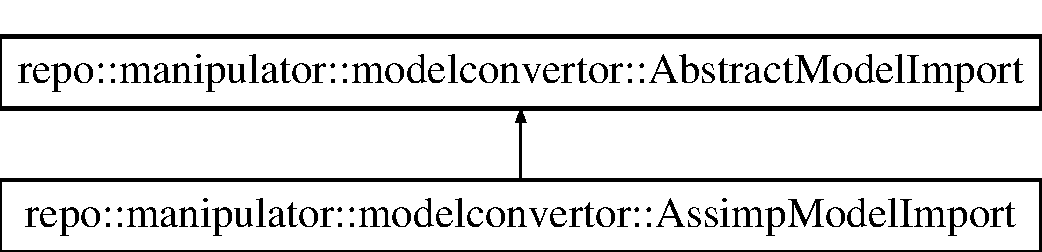
\includegraphics[height=2.000000cm]{classrepo_1_1manipulator_1_1modelconvertor_1_1_assimp_model_import}
\end{center}
\end{figure}
\subsection*{Public Member Functions}
\begin{DoxyCompactItemize}
\item 
\hyperlink{classrepo_1_1manipulator_1_1modelconvertor_1_1_assimp_model_import_a3d09c442384d4767b270384c9c9d8218}{Assimp\+Model\+Import} ()
\item 
\hyperlink{classrepo_1_1manipulator_1_1modelconvertor_1_1_assimp_model_import_abe3f60cfeb876fddc1752c13bf8f7616}{Assimp\+Model\+Import} (const \hyperlink{classrepo_1_1manipulator_1_1modelconvertor_1_1_model_import_config}{Model\+Import\+Config} $\ast$settings)
\item 
virtual \hyperlink{classrepo_1_1manipulator_1_1modelconvertor_1_1_assimp_model_import_acf7e9f1c6156170c92cb96d48853b6a7}{$\sim$\+Assimp\+Model\+Import} ()
\item 
\hyperlink{classrepo_1_1core_1_1model_1_1_repo_scene}{repo\+::core\+::model\+::\+Repo\+Scene} $\ast$ \hyperlink{classrepo_1_1manipulator_1_1modelconvertor_1_1_assimp_model_import_a5e51038056aee890d4860190ce8d5847}{generate\+Repo\+Scene} ()
\item 
bool \hyperlink{classrepo_1_1manipulator_1_1modelconvertor_1_1_assimp_model_import_aefdfec79f7be00e1ad452ee22555b64a}{import\+Model} (std\+::string file\+Path, std\+::string \&err\+Msg)
\end{DoxyCompactItemize}
\subsection*{Static Public Member Functions}
\begin{DoxyCompactItemize}
\item 
\hypertarget{classrepo_1_1manipulator_1_1modelconvertor_1_1_assimp_model_import_a31b1cd3f6004d51f6aec3edc8c49cb37}{}static std\+::string {\bfseries get\+Supported\+Formats} ()\label{classrepo_1_1manipulator_1_1modelconvertor_1_1_assimp_model_import_a31b1cd3f6004d51f6aec3edc8c49cb37}

\end{DoxyCompactItemize}
\subsection*{Additional Inherited Members}


\subsection{Constructor \& Destructor Documentation}
\hypertarget{classrepo_1_1manipulator_1_1modelconvertor_1_1_assimp_model_import_a3d09c442384d4767b270384c9c9d8218}{}\index{repo\+::manipulator\+::modelconvertor\+::\+Assimp\+Model\+Import@{repo\+::manipulator\+::modelconvertor\+::\+Assimp\+Model\+Import}!Assimp\+Model\+Import@{Assimp\+Model\+Import}}
\index{Assimp\+Model\+Import@{Assimp\+Model\+Import}!repo\+::manipulator\+::modelconvertor\+::\+Assimp\+Model\+Import@{repo\+::manipulator\+::modelconvertor\+::\+Assimp\+Model\+Import}}
\subsubsection[{Assimp\+Model\+Import}]{\setlength{\rightskip}{0pt plus 5cm}Assimp\+Model\+Import\+::\+Assimp\+Model\+Import (
\begin{DoxyParamCaption}
{}
\end{DoxyParamCaption}
)}\label{classrepo_1_1manipulator_1_1modelconvertor_1_1_assimp_model_import_a3d09c442384d4767b270384c9c9d8218}
Default Constructor, generate model with default settings \hypertarget{classrepo_1_1manipulator_1_1modelconvertor_1_1_assimp_model_import_abe3f60cfeb876fddc1752c13bf8f7616}{}\index{repo\+::manipulator\+::modelconvertor\+::\+Assimp\+Model\+Import@{repo\+::manipulator\+::modelconvertor\+::\+Assimp\+Model\+Import}!Assimp\+Model\+Import@{Assimp\+Model\+Import}}
\index{Assimp\+Model\+Import@{Assimp\+Model\+Import}!repo\+::manipulator\+::modelconvertor\+::\+Assimp\+Model\+Import@{repo\+::manipulator\+::modelconvertor\+::\+Assimp\+Model\+Import}}
\subsubsection[{Assimp\+Model\+Import}]{\setlength{\rightskip}{0pt plus 5cm}Assimp\+Model\+Import\+::\+Assimp\+Model\+Import (
\begin{DoxyParamCaption}
\item[{const {\bf Model\+Import\+Config} $\ast$}]{settings}
\end{DoxyParamCaption}
)}\label{classrepo_1_1manipulator_1_1modelconvertor_1_1_assimp_model_import_abe3f60cfeb876fddc1752c13bf8f7616}
Create \hyperlink{classrepo_1_1manipulator_1_1modelconvertor_1_1_assimp_model_import}{Assimp\+Model\+Import} with specific settings 
\begin{DoxyParams}{Parameters}
{\em settings} & \\
\hline
\end{DoxyParams}
\hypertarget{classrepo_1_1manipulator_1_1modelconvertor_1_1_assimp_model_import_acf7e9f1c6156170c92cb96d48853b6a7}{}\index{repo\+::manipulator\+::modelconvertor\+::\+Assimp\+Model\+Import@{repo\+::manipulator\+::modelconvertor\+::\+Assimp\+Model\+Import}!````~Assimp\+Model\+Import@{$\sim$\+Assimp\+Model\+Import}}
\index{````~Assimp\+Model\+Import@{$\sim$\+Assimp\+Model\+Import}!repo\+::manipulator\+::modelconvertor\+::\+Assimp\+Model\+Import@{repo\+::manipulator\+::modelconvertor\+::\+Assimp\+Model\+Import}}
\subsubsection[{$\sim$\+Assimp\+Model\+Import}]{\setlength{\rightskip}{0pt plus 5cm}Assimp\+Model\+Import\+::$\sim$\+Assimp\+Model\+Import (
\begin{DoxyParamCaption}
{}
\end{DoxyParamCaption}
)\hspace{0.3cm}{\ttfamily [virtual]}}\label{classrepo_1_1manipulator_1_1modelconvertor_1_1_assimp_model_import_acf7e9f1c6156170c92cb96d48853b6a7}
Default Deconstructor 

\subsection{Member Function Documentation}
\hypertarget{classrepo_1_1manipulator_1_1modelconvertor_1_1_assimp_model_import_a5e51038056aee890d4860190ce8d5847}{}\index{repo\+::manipulator\+::modelconvertor\+::\+Assimp\+Model\+Import@{repo\+::manipulator\+::modelconvertor\+::\+Assimp\+Model\+Import}!generate\+Repo\+Scene@{generate\+Repo\+Scene}}
\index{generate\+Repo\+Scene@{generate\+Repo\+Scene}!repo\+::manipulator\+::modelconvertor\+::\+Assimp\+Model\+Import@{repo\+::manipulator\+::modelconvertor\+::\+Assimp\+Model\+Import}}
\subsubsection[{generate\+Repo\+Scene}]{\setlength{\rightskip}{0pt plus 5cm}{\bf repo\+::core\+::model\+::\+Repo\+Scene} $\ast$ Assimp\+Model\+Import\+::generate\+Repo\+Scene (
\begin{DoxyParamCaption}
{}
\end{DoxyParamCaption}
)\hspace{0.3cm}{\ttfamily [virtual]}}\label{classrepo_1_1manipulator_1_1modelconvertor_1_1_assimp_model_import_a5e51038056aee890d4860190ce8d5847}
Generates a repo scene graph an internal representation(aiscene) needs to have been created before this call \begin{DoxyReturn}{Returns}
returns a populated Repo\+Scene upon success. 
\end{DoxyReturn}


Implements \hyperlink{classrepo_1_1manipulator_1_1modelconvertor_1_1_abstract_model_import_a0a0761d0a92ca05542b569a079f99c8f}{repo\+::manipulator\+::modelconvertor\+::\+Abstract\+Model\+Import}.

\hypertarget{classrepo_1_1manipulator_1_1modelconvertor_1_1_assimp_model_import_aefdfec79f7be00e1ad452ee22555b64a}{}\index{repo\+::manipulator\+::modelconvertor\+::\+Assimp\+Model\+Import@{repo\+::manipulator\+::modelconvertor\+::\+Assimp\+Model\+Import}!import\+Model@{import\+Model}}
\index{import\+Model@{import\+Model}!repo\+::manipulator\+::modelconvertor\+::\+Assimp\+Model\+Import@{repo\+::manipulator\+::modelconvertor\+::\+Assimp\+Model\+Import}}
\subsubsection[{import\+Model}]{\setlength{\rightskip}{0pt plus 5cm}bool Assimp\+Model\+Import\+::import\+Model (
\begin{DoxyParamCaption}
\item[{std\+::string}]{file\+Path, }
\item[{std\+::string \&}]{err\+Msg}
\end{DoxyParamCaption}
)\hspace{0.3cm}{\ttfamily [virtual]}}\label{classrepo_1_1manipulator_1_1modelconvertor_1_1_assimp_model_import_aefdfec79f7be00e1ad452ee22555b64a}
Import model from a given file 
\begin{DoxyParams}{Parameters}
{\em path} & to the file \\
\hline
{\em error} & message if failed \\
\hline
\end{DoxyParams}
\begin{DoxyReturn}{Returns}
returns true upon success 
\end{DoxyReturn}


Implements \hyperlink{classrepo_1_1manipulator_1_1modelconvertor_1_1_abstract_model_import_a2b6296ea483d39f7ce6fe1e8a78124fd}{repo\+::manipulator\+::modelconvertor\+::\+Abstract\+Model\+Import}.



The documentation for this class was generated from the following files\+:\begin{DoxyCompactItemize}
\item 
C\+:/\+Users/\+Carmen/3\+D Repo/\+Repo/3drepobouncer/bouncer/src/repo/manipulator/modelconvertor/import/repo\+\_\+model\+\_\+import\+\_\+assimp.\+h\item 
C\+:/\+Users/\+Carmen/3\+D Repo/\+Repo/3drepobouncer/bouncer/src/repo/manipulator/modelconvertor/import/repo\+\_\+model\+\_\+import\+\_\+assimp.\+cpp\end{DoxyCompactItemize}

\hypertarget{classrepo_1_1core_1_1model_1_1_camera_node}{}\section{repo\+:\+:core\+:\+:model\+:\+:Camera\+Node Class Reference}
\label{classrepo_1_1core_1_1model_1_1_camera_node}\index{repo\+::core\+::model\+::\+Camera\+Node@{repo\+::core\+::model\+::\+Camera\+Node}}
Inheritance diagram for repo\+:\+:core\+:\+:model\+:\+:Camera\+Node\+:\begin{figure}[H]
\begin{center}
\leavevmode
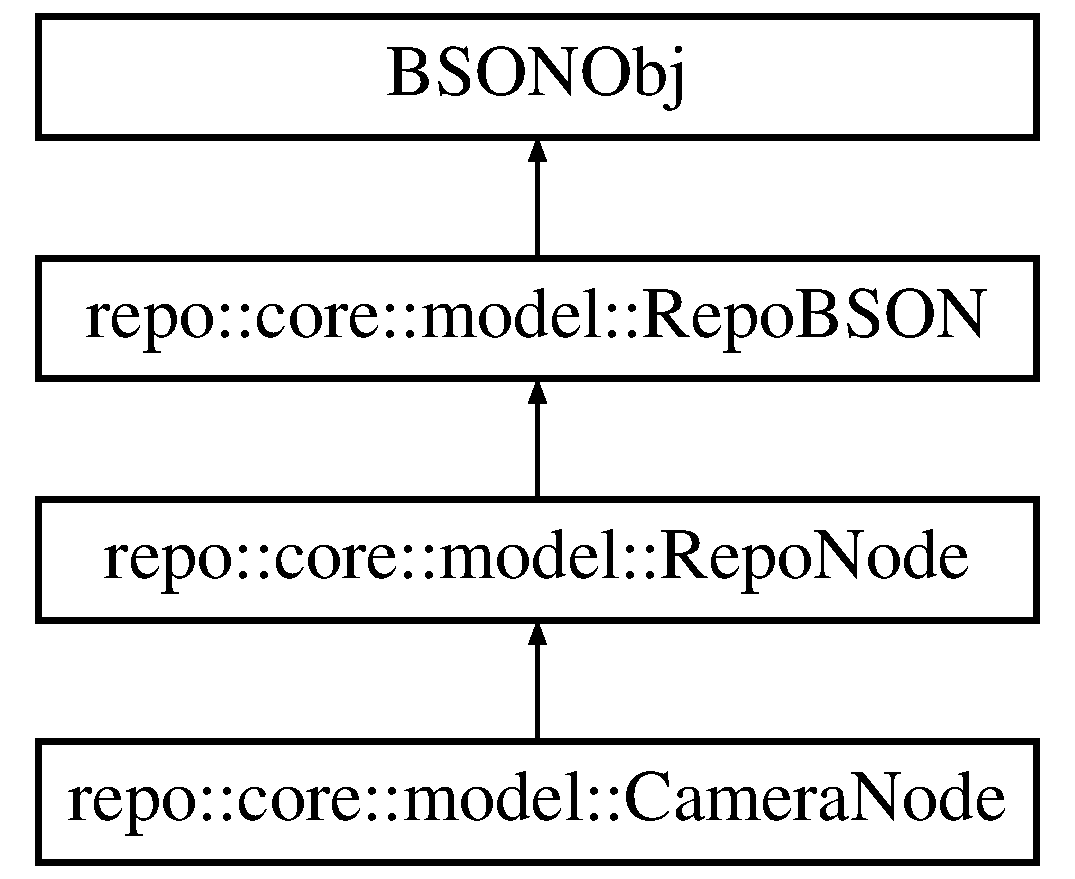
\includegraphics[height=4.000000cm]{classrepo_1_1core_1_1model_1_1_camera_node}
\end{center}
\end{figure}
\subsection*{Public Member Functions}
\begin{DoxyCompactItemize}
\item 
\hyperlink{classrepo_1_1core_1_1model_1_1_camera_node_a6e93f1af26050fe9ec35645785e29824}{Camera\+Node} ()
\item 
\hyperlink{classrepo_1_1core_1_1model_1_1_camera_node_a78aa6c32e17a3688e8490b69d7bb471a}{Camera\+Node} (\hyperlink{classrepo_1_1core_1_1model_1_1_repo_b_s_o_n}{Repo\+B\+S\+O\+N} bson)
\item 
\hyperlink{classrepo_1_1core_1_1model_1_1_camera_node_ab3a466dc9357b5200fb6843a6d64c5c8}{$\sim$\+Camera\+Node} ()
\item 
virtual bool \hyperlink{classrepo_1_1core_1_1model_1_1_camera_node_a5ff50e052f4266842e5d4e4840fe0c37}{position\+Dependant} ()
\item 
virtual \hyperlink{classrepo_1_1core_1_1model_1_1_repo_node}{Repo\+Node} \hyperlink{classrepo_1_1core_1_1model_1_1_camera_node_a98b1b2260da36fb75ff894c98df901cf}{clone\+And\+Apply\+Transformation} (const std\+::vector$<$ float $>$ \&matrix) const 
\item 
float \hyperlink{classrepo_1_1core_1_1model_1_1_camera_node_a49b27f160ea40eeb77e11c88e3a913d9}{get\+Aspect\+Ratio} () const 
\item 
float \hyperlink{classrepo_1_1core_1_1model_1_1_camera_node_a82d9fd39b1140e2d7e1ad3b6a4c1b753}{get\+Horizontal\+F\+O\+V} () const 
\item 
std\+::vector$<$ float $>$ \hyperlink{classrepo_1_1core_1_1model_1_1_camera_node_a7907960b05c955e3b56772bd09d9a919}{get\+Camera\+Matrix} (const bool \&row\+Major=true) const 
\item 
float \hyperlink{classrepo_1_1core_1_1model_1_1_camera_node_a321ee8fdfacf5705788b02c36b7cd391}{get\+Far\+Clipping\+Plane} () const 
\item 
float \hyperlink{classrepo_1_1core_1_1model_1_1_camera_node_aba3a69203e5c273a81d56a628498e21f}{get\+Field\+Of\+View} () const 
\item 
float \hyperlink{classrepo_1_1core_1_1model_1_1_camera_node_a7aae7ebc82db8fb039ab153bdd547cba}{get\+Near\+Clipping\+Plane} () const 
\item 
\hyperlink{structrepo__vector__t}{repo\+\_\+vector\+\_\+t} \hyperlink{classrepo_1_1core_1_1model_1_1_camera_node_a8cc4988da42d2eeaff46ed88c2291422}{get\+Look\+At} () const 
\item 
std\+::vector$<$ float $>$ \hyperlink{classrepo_1_1core_1_1model_1_1_camera_node_a34ada4c2ec02b855a188ee5007b8b606}{get\+Orientation} () const 
\item 
\hyperlink{structrepo__vector__t}{repo\+\_\+vector\+\_\+t} \hyperlink{classrepo_1_1core_1_1model_1_1_camera_node_a11441690bcd3f06884e084a1afc65ceb}{get\+Position} () const 
\item 
\hyperlink{structrepo__vector__t}{repo\+\_\+vector\+\_\+t} \hyperlink{classrepo_1_1core_1_1model_1_1_camera_node_a8812358773b363e5a30374b2344d3d71}{get\+Up} () const 
\item 
virtual bool \hyperlink{classrepo_1_1core_1_1model_1_1_camera_node_a4d4a8875d7929aa92beedd9bd0eeea63}{s\+Equal} (const \hyperlink{classrepo_1_1core_1_1model_1_1_repo_node}{Repo\+Node} \&other) const 
\end{DoxyCompactItemize}
\subsection*{Additional Inherited Members}


\subsection{Constructor \& Destructor Documentation}
\hypertarget{classrepo_1_1core_1_1model_1_1_camera_node_a6e93f1af26050fe9ec35645785e29824}{}\index{repo\+::core\+::model\+::\+Camera\+Node@{repo\+::core\+::model\+::\+Camera\+Node}!Camera\+Node@{Camera\+Node}}
\index{Camera\+Node@{Camera\+Node}!repo\+::core\+::model\+::\+Camera\+Node@{repo\+::core\+::model\+::\+Camera\+Node}}
\subsubsection[{Camera\+Node}]{\setlength{\rightskip}{0pt plus 5cm}Camera\+Node\+::\+Camera\+Node (
\begin{DoxyParamCaption}
{}
\end{DoxyParamCaption}
)}\label{classrepo_1_1core_1_1model_1_1_camera_node_a6e93f1af26050fe9ec35645785e29824}
Default constructor \hypertarget{classrepo_1_1core_1_1model_1_1_camera_node_a78aa6c32e17a3688e8490b69d7bb471a}{}\index{repo\+::core\+::model\+::\+Camera\+Node@{repo\+::core\+::model\+::\+Camera\+Node}!Camera\+Node@{Camera\+Node}}
\index{Camera\+Node@{Camera\+Node}!repo\+::core\+::model\+::\+Camera\+Node@{repo\+::core\+::model\+::\+Camera\+Node}}
\subsubsection[{Camera\+Node}]{\setlength{\rightskip}{0pt plus 5cm}Camera\+Node\+::\+Camera\+Node (
\begin{DoxyParamCaption}
\item[{{\bf Repo\+B\+S\+O\+N}}]{bson}
\end{DoxyParamCaption}
)}\label{classrepo_1_1core_1_1model_1_1_camera_node_a78aa6c32e17a3688e8490b69d7bb471a}
Construct a \hyperlink{classrepo_1_1core_1_1model_1_1_camera_node}{Camera\+Node} from a \hyperlink{classrepo_1_1core_1_1model_1_1_repo_b_s_o_n}{Repo\+B\+S\+O\+N} object 
\begin{DoxyParams}{Parameters}
{\em \hyperlink{classrepo_1_1core_1_1model_1_1_repo_b_s_o_n}{Repo\+B\+S\+O\+N}} & object \\
\hline
\end{DoxyParams}
\hypertarget{classrepo_1_1core_1_1model_1_1_camera_node_ab3a466dc9357b5200fb6843a6d64c5c8}{}\index{repo\+::core\+::model\+::\+Camera\+Node@{repo\+::core\+::model\+::\+Camera\+Node}!````~Camera\+Node@{$\sim$\+Camera\+Node}}
\index{````~Camera\+Node@{$\sim$\+Camera\+Node}!repo\+::core\+::model\+::\+Camera\+Node@{repo\+::core\+::model\+::\+Camera\+Node}}
\subsubsection[{$\sim$\+Camera\+Node}]{\setlength{\rightskip}{0pt plus 5cm}Camera\+Node\+::$\sim$\+Camera\+Node (
\begin{DoxyParamCaption}
{}
\end{DoxyParamCaption}
)}\label{classrepo_1_1core_1_1model_1_1_camera_node_ab3a466dc9357b5200fb6843a6d64c5c8}
Default deconstructor 

\subsection{Member Function Documentation}
\hypertarget{classrepo_1_1core_1_1model_1_1_camera_node_a98b1b2260da36fb75ff894c98df901cf}{}\index{repo\+::core\+::model\+::\+Camera\+Node@{repo\+::core\+::model\+::\+Camera\+Node}!clone\+And\+Apply\+Transformation@{clone\+And\+Apply\+Transformation}}
\index{clone\+And\+Apply\+Transformation@{clone\+And\+Apply\+Transformation}!repo\+::core\+::model\+::\+Camera\+Node@{repo\+::core\+::model\+::\+Camera\+Node}}
\subsubsection[{clone\+And\+Apply\+Transformation}]{\setlength{\rightskip}{0pt plus 5cm}{\bf Repo\+Node} Camera\+Node\+::clone\+And\+Apply\+Transformation (
\begin{DoxyParamCaption}
\item[{const std\+::vector$<$ float $>$ \&}]{matrix}
\end{DoxyParamCaption}
) const\hspace{0.3cm}{\ttfamily [virtual]}}\label{classrepo_1_1core_1_1model_1_1_camera_node_a98b1b2260da36fb75ff894c98df901cf}
Create a new object with transformation applied to the node default behaviour is do nothing. Children object needs to override this function to perform their own specific behaviour. 
\begin{DoxyParams}{Parameters}
{\em matrix} & transformation matrix to apply. \\
\hline
\end{DoxyParams}
\begin{DoxyReturn}{Returns}
returns a new object with transformation applied. 
\end{DoxyReturn}


Reimplemented from \hyperlink{classrepo_1_1core_1_1model_1_1_repo_node_ac31acdb9774bce9296cb5005286db83d}{repo\+::core\+::model\+::\+Repo\+Node}.

\hypertarget{classrepo_1_1core_1_1model_1_1_camera_node_a49b27f160ea40eeb77e11c88e3a913d9}{}\index{repo\+::core\+::model\+::\+Camera\+Node@{repo\+::core\+::model\+::\+Camera\+Node}!get\+Aspect\+Ratio@{get\+Aspect\+Ratio}}
\index{get\+Aspect\+Ratio@{get\+Aspect\+Ratio}!repo\+::core\+::model\+::\+Camera\+Node@{repo\+::core\+::model\+::\+Camera\+Node}}
\subsubsection[{get\+Aspect\+Ratio}]{\setlength{\rightskip}{0pt plus 5cm}float repo\+::core\+::model\+::\+Camera\+Node\+::get\+Aspect\+Ratio (
\begin{DoxyParamCaption}
{}
\end{DoxyParamCaption}
) const\hspace{0.3cm}{\ttfamily [inline]}}\label{classrepo_1_1core_1_1model_1_1_camera_node_a49b27f160ea40eeb77e11c88e3a913d9}
-\/-\/-\/------ Convenience functions -\/-\/-\/-\/-\/------ Get aspect ratio \begin{DoxyReturn}{Returns}
returns the 4 by 4 matrix as a vector 
\end{DoxyReturn}
\hypertarget{classrepo_1_1core_1_1model_1_1_camera_node_a7907960b05c955e3b56772bd09d9a919}{}\index{repo\+::core\+::model\+::\+Camera\+Node@{repo\+::core\+::model\+::\+Camera\+Node}!get\+Camera\+Matrix@{get\+Camera\+Matrix}}
\index{get\+Camera\+Matrix@{get\+Camera\+Matrix}!repo\+::core\+::model\+::\+Camera\+Node@{repo\+::core\+::model\+::\+Camera\+Node}}
\subsubsection[{get\+Camera\+Matrix}]{\setlength{\rightskip}{0pt plus 5cm}std\+::vector$<$ float $>$ Camera\+Node\+::get\+Camera\+Matrix (
\begin{DoxyParamCaption}
\item[{const bool \&}]{row\+Major = {\ttfamily true}}
\end{DoxyParamCaption}
) const}\label{classrepo_1_1core_1_1model_1_1_camera_node_a7907960b05c955e3b56772bd09d9a919}
Get the 4 by 4 camera matrix 
\begin{DoxyParams}{Parameters}
{\em true} & if row major (row is the fast dimension) \\
\hline
\end{DoxyParams}
\begin{DoxyReturn}{Returns}
returns the 4 by 4 matrix as a vector 
\end{DoxyReturn}
We don\textquotesingle{}t know whether these vectors are already normalized ... \hypertarget{classrepo_1_1core_1_1model_1_1_camera_node_a321ee8fdfacf5705788b02c36b7cd391}{}\index{repo\+::core\+::model\+::\+Camera\+Node@{repo\+::core\+::model\+::\+Camera\+Node}!get\+Far\+Clipping\+Plane@{get\+Far\+Clipping\+Plane}}
\index{get\+Far\+Clipping\+Plane@{get\+Far\+Clipping\+Plane}!repo\+::core\+::model\+::\+Camera\+Node@{repo\+::core\+::model\+::\+Camera\+Node}}
\subsubsection[{get\+Far\+Clipping\+Plane}]{\setlength{\rightskip}{0pt plus 5cm}float repo\+::core\+::model\+::\+Camera\+Node\+::get\+Far\+Clipping\+Plane (
\begin{DoxyParamCaption}
{}
\end{DoxyParamCaption}
) const\hspace{0.3cm}{\ttfamily [inline]}}\label{classrepo_1_1core_1_1model_1_1_camera_node_a321ee8fdfacf5705788b02c36b7cd391}
Return the value for far clipping plane \begin{DoxyReturn}{Returns}
returns the value for far clipping plane 
\end{DoxyReturn}
\hypertarget{classrepo_1_1core_1_1model_1_1_camera_node_aba3a69203e5c273a81d56a628498e21f}{}\index{repo\+::core\+::model\+::\+Camera\+Node@{repo\+::core\+::model\+::\+Camera\+Node}!get\+Field\+Of\+View@{get\+Field\+Of\+View}}
\index{get\+Field\+Of\+View@{get\+Field\+Of\+View}!repo\+::core\+::model\+::\+Camera\+Node@{repo\+::core\+::model\+::\+Camera\+Node}}
\subsubsection[{get\+Field\+Of\+View}]{\setlength{\rightskip}{0pt plus 5cm}float repo\+::core\+::model\+::\+Camera\+Node\+::get\+Field\+Of\+View (
\begin{DoxyParamCaption}
{}
\end{DoxyParamCaption}
) const\hspace{0.3cm}{\ttfamily [inline]}}\label{classrepo_1_1core_1_1model_1_1_camera_node_aba3a69203e5c273a81d56a628498e21f}
Return the value for field of view \begin{DoxyReturn}{Returns}
returns the value for field\+Of\+View 
\end{DoxyReturn}
\hypertarget{classrepo_1_1core_1_1model_1_1_camera_node_a82d9fd39b1140e2d7e1ad3b6a4c1b753}{}\index{repo\+::core\+::model\+::\+Camera\+Node@{repo\+::core\+::model\+::\+Camera\+Node}!get\+Horizontal\+F\+O\+V@{get\+Horizontal\+F\+O\+V}}
\index{get\+Horizontal\+F\+O\+V@{get\+Horizontal\+F\+O\+V}!repo\+::core\+::model\+::\+Camera\+Node@{repo\+::core\+::model\+::\+Camera\+Node}}
\subsubsection[{get\+Horizontal\+F\+O\+V}]{\setlength{\rightskip}{0pt plus 5cm}float repo\+::core\+::model\+::\+Camera\+Node\+::get\+Horizontal\+F\+O\+V (
\begin{DoxyParamCaption}
{}
\end{DoxyParamCaption}
) const\hspace{0.3cm}{\ttfamily [inline]}}\label{classrepo_1_1core_1_1model_1_1_camera_node_a82d9fd39b1140e2d7e1ad3b6a4c1b753}
Get horiztonal F\+O\+V \begin{DoxyReturn}{Returns}
returns the 4 by 4 matrix as a vector 
\end{DoxyReturn}
\hypertarget{classrepo_1_1core_1_1model_1_1_camera_node_a8cc4988da42d2eeaff46ed88c2291422}{}\index{repo\+::core\+::model\+::\+Camera\+Node@{repo\+::core\+::model\+::\+Camera\+Node}!get\+Look\+At@{get\+Look\+At}}
\index{get\+Look\+At@{get\+Look\+At}!repo\+::core\+::model\+::\+Camera\+Node@{repo\+::core\+::model\+::\+Camera\+Node}}
\subsubsection[{get\+Look\+At}]{\setlength{\rightskip}{0pt plus 5cm}{\bf repo\+\_\+vector\+\_\+t} Camera\+Node\+::get\+Look\+At (
\begin{DoxyParamCaption}
{}
\end{DoxyParamCaption}
) const}\label{classrepo_1_1core_1_1model_1_1_camera_node_a8cc4988da42d2eeaff46ed88c2291422}
Get the Look At vector of the camera \begin{DoxyReturn}{Returns}
returns a vector of the \char`\"{}\+Look At\char`\"{} 
\end{DoxyReturn}
\hypertarget{classrepo_1_1core_1_1model_1_1_camera_node_a7aae7ebc82db8fb039ab153bdd547cba}{}\index{repo\+::core\+::model\+::\+Camera\+Node@{repo\+::core\+::model\+::\+Camera\+Node}!get\+Near\+Clipping\+Plane@{get\+Near\+Clipping\+Plane}}
\index{get\+Near\+Clipping\+Plane@{get\+Near\+Clipping\+Plane}!repo\+::core\+::model\+::\+Camera\+Node@{repo\+::core\+::model\+::\+Camera\+Node}}
\subsubsection[{get\+Near\+Clipping\+Plane}]{\setlength{\rightskip}{0pt plus 5cm}float repo\+::core\+::model\+::\+Camera\+Node\+::get\+Near\+Clipping\+Plane (
\begin{DoxyParamCaption}
{}
\end{DoxyParamCaption}
) const\hspace{0.3cm}{\ttfamily [inline]}}\label{classrepo_1_1core_1_1model_1_1_camera_node_a7aae7ebc82db8fb039ab153bdd547cba}
Return the value for near clipping plane \begin{DoxyReturn}{Returns}
returns the value for near clipping plane 
\end{DoxyReturn}
\hypertarget{classrepo_1_1core_1_1model_1_1_camera_node_a34ada4c2ec02b855a188ee5007b8b606}{}\index{repo\+::core\+::model\+::\+Camera\+Node@{repo\+::core\+::model\+::\+Camera\+Node}!get\+Orientation@{get\+Orientation}}
\index{get\+Orientation@{get\+Orientation}!repo\+::core\+::model\+::\+Camera\+Node@{repo\+::core\+::model\+::\+Camera\+Node}}
\subsubsection[{get\+Orientation}]{\setlength{\rightskip}{0pt plus 5cm}std\+::vector$<$ float $>$ Camera\+Node\+::get\+Orientation (
\begin{DoxyParamCaption}
{}
\end{DoxyParamCaption}
) const}\label{classrepo_1_1core_1_1model_1_1_camera_node_a34ada4c2ec02b855a188ee5007b8b606}
get the orientation of the camera \begin{DoxyReturn}{Returns}
returns a vector with 4 fields, \{x, y, z, angle\} 
\end{DoxyReturn}
\hypertarget{classrepo_1_1core_1_1model_1_1_camera_node_a11441690bcd3f06884e084a1afc65ceb}{}\index{repo\+::core\+::model\+::\+Camera\+Node@{repo\+::core\+::model\+::\+Camera\+Node}!get\+Position@{get\+Position}}
\index{get\+Position@{get\+Position}!repo\+::core\+::model\+::\+Camera\+Node@{repo\+::core\+::model\+::\+Camera\+Node}}
\subsubsection[{get\+Position}]{\setlength{\rightskip}{0pt plus 5cm}{\bf repo\+\_\+vector\+\_\+t} Camera\+Node\+::get\+Position (
\begin{DoxyParamCaption}
{}
\end{DoxyParamCaption}
) const}\label{classrepo_1_1core_1_1model_1_1_camera_node_a11441690bcd3f06884e084a1afc65ceb}
Get the position of the camera \begin{DoxyReturn}{Returns}
returns a vector of the position 
\end{DoxyReturn}
\hypertarget{classrepo_1_1core_1_1model_1_1_camera_node_a8812358773b363e5a30374b2344d3d71}{}\index{repo\+::core\+::model\+::\+Camera\+Node@{repo\+::core\+::model\+::\+Camera\+Node}!get\+Up@{get\+Up}}
\index{get\+Up@{get\+Up}!repo\+::core\+::model\+::\+Camera\+Node@{repo\+::core\+::model\+::\+Camera\+Node}}
\subsubsection[{get\+Up}]{\setlength{\rightskip}{0pt plus 5cm}{\bf repo\+\_\+vector\+\_\+t} Camera\+Node\+::get\+Up (
\begin{DoxyParamCaption}
{}
\end{DoxyParamCaption}
) const}\label{classrepo_1_1core_1_1model_1_1_camera_node_a8812358773b363e5a30374b2344d3d71}
Get the up vector of the camera \begin{DoxyReturn}{Returns}
returns a vector of up 
\end{DoxyReturn}
\hypertarget{classrepo_1_1core_1_1model_1_1_camera_node_a5ff50e052f4266842e5d4e4840fe0c37}{}\index{repo\+::core\+::model\+::\+Camera\+Node@{repo\+::core\+::model\+::\+Camera\+Node}!position\+Dependant@{position\+Dependant}}
\index{position\+Dependant@{position\+Dependant}!repo\+::core\+::model\+::\+Camera\+Node@{repo\+::core\+::model\+::\+Camera\+Node}}
\subsubsection[{position\+Dependant}]{\setlength{\rightskip}{0pt plus 5cm}virtual bool repo\+::core\+::model\+::\+Camera\+Node\+::position\+Dependant (
\begin{DoxyParamCaption}
{}
\end{DoxyParamCaption}
)\hspace{0.3cm}{\ttfamily [inline]}, {\ttfamily [virtual]}}\label{classrepo_1_1core_1_1model_1_1_camera_node_a5ff50e052f4266842e5d4e4840fe0c37}
Check if the node is position dependant. i.\+e. if parent transformation is merged onto the node, does the node requre to a transformation applied to it e.\+g. meshes and cameras are position dependant, metadata isn\textquotesingle{}t Default behaviour is false. Position dependant child requires override this function. \begin{DoxyReturn}{Returns}
true if node is position\+Dependant. 
\end{DoxyReturn}


Reimplemented from \hyperlink{classrepo_1_1core_1_1model_1_1_repo_node_aa3e0f98690dc8bfe082d2fc57b904798}{repo\+::core\+::model\+::\+Repo\+Node}.

\hypertarget{classrepo_1_1core_1_1model_1_1_camera_node_a4d4a8875d7929aa92beedd9bd0eeea63}{}\index{repo\+::core\+::model\+::\+Camera\+Node@{repo\+::core\+::model\+::\+Camera\+Node}!s\+Equal@{s\+Equal}}
\index{s\+Equal@{s\+Equal}!repo\+::core\+::model\+::\+Camera\+Node@{repo\+::core\+::model\+::\+Camera\+Node}}
\subsubsection[{s\+Equal}]{\setlength{\rightskip}{0pt plus 5cm}bool Camera\+Node\+::s\+Equal (
\begin{DoxyParamCaption}
\item[{const {\bf Repo\+Node} \&}]{other}
\end{DoxyParamCaption}
) const\hspace{0.3cm}{\ttfamily [virtual]}}\label{classrepo_1_1core_1_1model_1_1_camera_node_a4d4a8875d7929aa92beedd9bd0eeea63}
Check if the node is semantically equal to another Different node should have a different interpretation of what this means. 
\begin{DoxyParams}{Parameters}
{\em other} & node to compare with \\
\hline
{\em returns} & true if equal, false otherwise \\
\hline
\end{DoxyParams}


Reimplemented from \hyperlink{classrepo_1_1core_1_1model_1_1_repo_node_a7c98830a876ee6516587a8f07c7015a5}{repo\+::core\+::model\+::\+Repo\+Node}.



The documentation for this class was generated from the following files\+:\begin{DoxyCompactItemize}
\item 
C\+:/\+Users/\+Carmen/3\+D Repo/\+Repo/3drepobouncer/bouncer/src/repo/core/model/bson/repo\+\_\+node\+\_\+camera.\+h\item 
C\+:/\+Users/\+Carmen/3\+D Repo/\+Repo/3drepobouncer/bouncer/src/repo/core/model/bson/repo\+\_\+node\+\_\+camera.\+cpp\end{DoxyCompactItemize}

\hypertarget{classrepo_1_1core_1_1model_1_1_collection_stats}{}\section{repo\+:\+:core\+:\+:model\+:\+:Collection\+Stats Class Reference}
\label{classrepo_1_1core_1_1model_1_1_collection_stats}\index{repo\+::core\+::model\+::\+Collection\+Stats@{repo\+::core\+::model\+::\+Collection\+Stats}}
Inheritance diagram for repo\+:\+:core\+:\+:model\+:\+:Collection\+Stats\+:\begin{figure}[H]
\begin{center}
\leavevmode
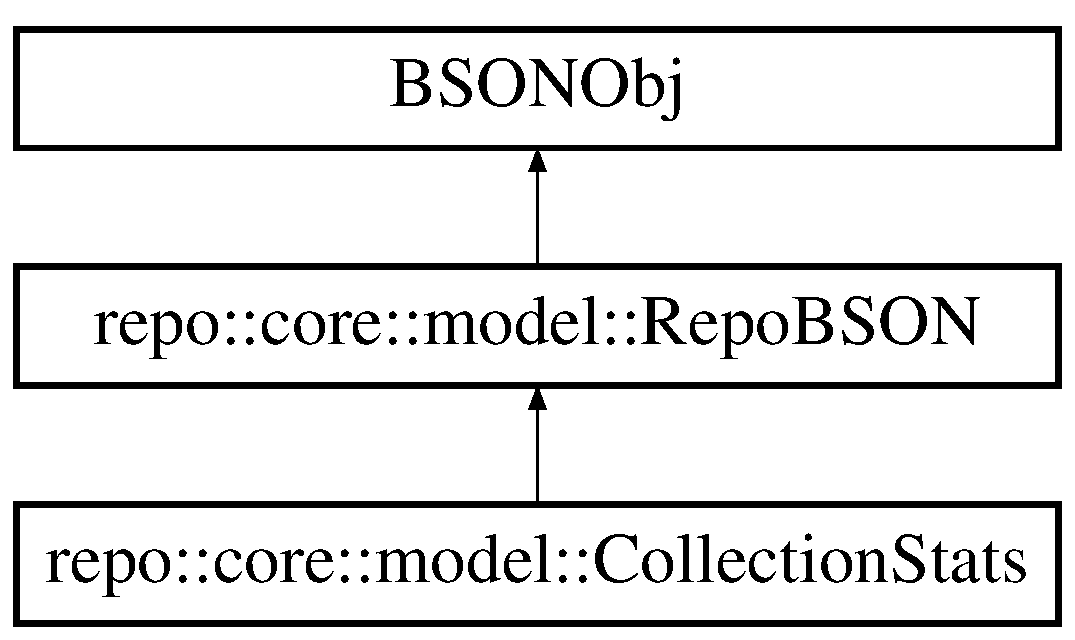
\includegraphics[height=3.000000cm]{classrepo_1_1core_1_1model_1_1_collection_stats}
\end{center}
\end{figure}
\subsection*{Public Member Functions}
\begin{DoxyCompactItemize}
\item 
\hyperlink{classrepo_1_1core_1_1model_1_1_collection_stats_a6082e14c62edad60af083492e0600427}{Collection\+Stats} ()
\item 
\hypertarget{classrepo_1_1core_1_1model_1_1_collection_stats_a47aa1933248bfe322a1ad9e0cddf8cd2}{}{\bfseries Collection\+Stats} (\hyperlink{classrepo_1_1core_1_1model_1_1_repo_b_s_o_n}{Repo\+B\+S\+O\+N} bson)\label{classrepo_1_1core_1_1model_1_1_collection_stats_a47aa1933248bfe322a1ad9e0cddf8cd2}

\item 
\hyperlink{classrepo_1_1core_1_1model_1_1_collection_stats_a921b8ddd4297b58049fc22157d932e63}{$\sim$\+Collection\+Stats} ()
\item 
\hypertarget{classrepo_1_1core_1_1model_1_1_collection_stats_a657733d44da987904d788e17026652b1}{}uint64\+\_\+t \hyperlink{classrepo_1_1core_1_1model_1_1_collection_stats_a657733d44da987904d788e17026652b1}{get\+Actual\+Size\+On\+Disk} () const \label{classrepo_1_1core_1_1model_1_1_collection_stats_a657733d44da987904d788e17026652b1}

\begin{DoxyCompactList}\small\item\em Actual size on disk. \end{DoxyCompactList}\item 
\hypertarget{classrepo_1_1core_1_1model_1_1_collection_stats_ab6e59940dacdd412f6409bf98f4dad30}{}std\+::string \hyperlink{classrepo_1_1core_1_1model_1_1_collection_stats_ab6e59940dacdd412f6409bf98f4dad30}{get\+Database} () const \label{classrepo_1_1core_1_1model_1_1_collection_stats_ab6e59940dacdd412f6409bf98f4dad30}

\begin{DoxyCompactList}\small\item\em Returns database. \end{DoxyCompactList}\item 
\hypertarget{classrepo_1_1core_1_1model_1_1_collection_stats_a7465b17cdc97afab486f40c8102378ba}{}uint64\+\_\+t \hyperlink{classrepo_1_1core_1_1model_1_1_collection_stats_a7465b17cdc97afab486f40c8102378ba}{get\+Count} () const \label{classrepo_1_1core_1_1model_1_1_collection_stats_a7465b17cdc97afab486f40c8102378ba}

\begin{DoxyCompactList}\small\item\em Returns the number of objects or documents in this collection. \end{DoxyCompactList}\item 
\hypertarget{classrepo_1_1core_1_1model_1_1_collection_stats_a2c7bcea557ae2c72ecd91773679e4a74}{}std\+::string \hyperlink{classrepo_1_1core_1_1model_1_1_collection_stats_a2c7bcea557ae2c72ecd91773679e4a74}{get\+Collection} () const \label{classrepo_1_1core_1_1model_1_1_collection_stats_a2c7bcea557ae2c72ecd91773679e4a74}

\begin{DoxyCompactList}\small\item\em Returns collection. \end{DoxyCompactList}\item 
\hypertarget{classrepo_1_1core_1_1model_1_1_collection_stats_a7fccb756d09201d837083b8dff2cce6a}{}std\+::string \hyperlink{classrepo_1_1core_1_1model_1_1_collection_stats_a7fccb756d09201d837083b8dff2cce6a}{get\+Ns} () const \label{classrepo_1_1core_1_1model_1_1_collection_stats_a7fccb756d09201d837083b8dff2cce6a}

\begin{DoxyCompactList}\small\item\em Returns namespace. \end{DoxyCompactList}\item 
\hypertarget{classrepo_1_1core_1_1model_1_1_collection_stats_a194999e73853f9ca9839d45dee999695}{}uint64\+\_\+t \hyperlink{classrepo_1_1core_1_1model_1_1_collection_stats_a194999e73853f9ca9839d45dee999695}{get\+Size} (const std\+::string \&name) const \label{classrepo_1_1core_1_1model_1_1_collection_stats_a194999e73853f9ca9839d45dee999695}

\begin{DoxyCompactList}\small\item\em Returns different sizes depending on name. \end{DoxyCompactList}\item 
uint64\+\_\+t \hyperlink{classrepo_1_1core_1_1model_1_1_collection_stats_aa7d520454a7f55bf364462b50ab885dc}{get\+Size} () const 
\item 
uint64\+\_\+t \hyperlink{classrepo_1_1core_1_1model_1_1_collection_stats_a5691eda860be3ab565bb2269d8640fbc}{get\+Storage\+Size} () const 
\item 
uint64\+\_\+t \hyperlink{classrepo_1_1core_1_1model_1_1_collection_stats_ad960d1732c85fedcdda72de8ad75e214}{get\+Total\+Index\+Size} () const 
\end{DoxyCompactItemize}
\subsection*{Static Public Member Functions}
\begin{DoxyCompactItemize}
\item 
\hypertarget{classrepo_1_1core_1_1model_1_1_collection_stats_a093b82f913cb8f03329809a02e650578}{}static std\+::string \hyperlink{classrepo_1_1core_1_1model_1_1_collection_stats_a093b82f913cb8f03329809a02e650578}{get\+Database} (const std\+::string \&ns)\label{classrepo_1_1core_1_1model_1_1_collection_stats_a093b82f913cb8f03329809a02e650578}

\begin{DoxyCompactList}\small\item\em Returns database from given namespace. \end{DoxyCompactList}\item 
\hypertarget{classrepo_1_1core_1_1model_1_1_collection_stats_a983ab226764884fbf99b55f644678e0a}{}static std\+::string \hyperlink{classrepo_1_1core_1_1model_1_1_collection_stats_a983ab226764884fbf99b55f644678e0a}{get\+Collection} (const std\+::string \&ns)\label{classrepo_1_1core_1_1model_1_1_collection_stats_a983ab226764884fbf99b55f644678e0a}

\begin{DoxyCompactList}\small\item\em Returns collection from given namespace. \end{DoxyCompactList}\end{DoxyCompactItemize}
\subsection*{Additional Inherited Members}


\subsection{Constructor \& Destructor Documentation}
\hypertarget{classrepo_1_1core_1_1model_1_1_collection_stats_a6082e14c62edad60af083492e0600427}{}\index{repo\+::core\+::model\+::\+Collection\+Stats@{repo\+::core\+::model\+::\+Collection\+Stats}!Collection\+Stats@{Collection\+Stats}}
\index{Collection\+Stats@{Collection\+Stats}!repo\+::core\+::model\+::\+Collection\+Stats@{repo\+::core\+::model\+::\+Collection\+Stats}}
\subsubsection[{Collection\+Stats}]{\setlength{\rightskip}{0pt plus 5cm}Collection\+Stats\+::\+Collection\+Stats (
\begin{DoxyParamCaption}
{}
\end{DoxyParamCaption}
)}\label{classrepo_1_1core_1_1model_1_1_collection_stats_a6082e14c62edad60af083492e0600427}
Default Constructor \hypertarget{classrepo_1_1core_1_1model_1_1_collection_stats_a921b8ddd4297b58049fc22157d932e63}{}\index{repo\+::core\+::model\+::\+Collection\+Stats@{repo\+::core\+::model\+::\+Collection\+Stats}!````~Collection\+Stats@{$\sim$\+Collection\+Stats}}
\index{````~Collection\+Stats@{$\sim$\+Collection\+Stats}!repo\+::core\+::model\+::\+Collection\+Stats@{repo\+::core\+::model\+::\+Collection\+Stats}}
\subsubsection[{$\sim$\+Collection\+Stats}]{\setlength{\rightskip}{0pt plus 5cm}Collection\+Stats\+::$\sim$\+Collection\+Stats (
\begin{DoxyParamCaption}
{}
\end{DoxyParamCaption}
)}\label{classrepo_1_1core_1_1model_1_1_collection_stats_a921b8ddd4297b58049fc22157d932e63}
Destructor 

\subsection{Member Function Documentation}
\hypertarget{classrepo_1_1core_1_1model_1_1_collection_stats_aa7d520454a7f55bf364462b50ab885dc}{}\index{repo\+::core\+::model\+::\+Collection\+Stats@{repo\+::core\+::model\+::\+Collection\+Stats}!get\+Size@{get\+Size}}
\index{get\+Size@{get\+Size}!repo\+::core\+::model\+::\+Collection\+Stats@{repo\+::core\+::model\+::\+Collection\+Stats}}
\subsubsection[{get\+Size}]{\setlength{\rightskip}{0pt plus 5cm}uint64\+\_\+t repo\+::core\+::model\+::\+Collection\+Stats\+::get\+Size (
\begin{DoxyParamCaption}
{}
\end{DoxyParamCaption}
) const}\label{classrepo_1_1core_1_1model_1_1_collection_stats_aa7d520454a7f55bf364462b50ab885dc}
Returns the total size of all records in a collection. This value does not include the record header, which is 16 bytes per record, but does include the record�s padding. Additionally, size does not include the size of any indexes associated with the collection, which the total\+Index\+Size field reports.

See \href{http://docs.mongodb.org/manual/reference/command/collStats/#collStats.size}{\tt http\+://docs.\+mongodb.\+org/manual/reference/command/coll\+Stats/\#coll\+Stats.\+size} \hypertarget{classrepo_1_1core_1_1model_1_1_collection_stats_a5691eda860be3ab565bb2269d8640fbc}{}\index{repo\+::core\+::model\+::\+Collection\+Stats@{repo\+::core\+::model\+::\+Collection\+Stats}!get\+Storage\+Size@{get\+Storage\+Size}}
\index{get\+Storage\+Size@{get\+Storage\+Size}!repo\+::core\+::model\+::\+Collection\+Stats@{repo\+::core\+::model\+::\+Collection\+Stats}}
\subsubsection[{get\+Storage\+Size}]{\setlength{\rightskip}{0pt plus 5cm}uint64\+\_\+t repo\+::core\+::model\+::\+Collection\+Stats\+::get\+Storage\+Size (
\begin{DoxyParamCaption}
{}
\end{DoxyParamCaption}
) const}\label{classrepo_1_1core_1_1model_1_1_collection_stats_a5691eda860be3ab565bb2269d8640fbc}
Returns the total amount of storage allocated to this collection for document storage.

See\+: \href{http://docs.mongodb.org/manual/reference/command/collStats/#collStats.storageSize}{\tt http\+://docs.\+mongodb.\+org/manual/reference/command/coll\+Stats/\#coll\+Stats.\+storage\+Size} \hypertarget{classrepo_1_1core_1_1model_1_1_collection_stats_ad960d1732c85fedcdda72de8ad75e214}{}\index{repo\+::core\+::model\+::\+Collection\+Stats@{repo\+::core\+::model\+::\+Collection\+Stats}!get\+Total\+Index\+Size@{get\+Total\+Index\+Size}}
\index{get\+Total\+Index\+Size@{get\+Total\+Index\+Size}!repo\+::core\+::model\+::\+Collection\+Stats@{repo\+::core\+::model\+::\+Collection\+Stats}}
\subsubsection[{get\+Total\+Index\+Size}]{\setlength{\rightskip}{0pt plus 5cm}uint64\+\_\+t repo\+::core\+::model\+::\+Collection\+Stats\+::get\+Total\+Index\+Size (
\begin{DoxyParamCaption}
{}
\end{DoxyParamCaption}
) const}\label{classrepo_1_1core_1_1model_1_1_collection_stats_ad960d1732c85fedcdda72de8ad75e214}
Returns the total size of all indexes. 

The documentation for this class was generated from the following files\+:\begin{DoxyCompactItemize}
\item 
C\+:/\+Users/\+Carmen/3\+D Repo/\+Repo/3drepobouncer/bouncer/src/repo/core/model/bson/repo\+\_\+bson\+\_\+collection\+\_\+stats.\+h\item 
C\+:/\+Users/\+Carmen/3\+D Repo/\+Repo/3drepobouncer/bouncer/src/repo/core/model/bson/repo\+\_\+bson\+\_\+collection\+\_\+stats.\+cpp\end{DoxyCompactItemize}

\hypertarget{classrepo_1_1manipulator_1_1diff_1_1_diff_by_name}{}\section{repo\+:\+:manipulator\+:\+:diff\+:\+:Diff\+By\+Name Class Reference}
\label{classrepo_1_1manipulator_1_1diff_1_1_diff_by_name}\index{repo\+::manipulator\+::diff\+::\+Diff\+By\+Name@{repo\+::manipulator\+::diff\+::\+Diff\+By\+Name}}
Inheritance diagram for repo\+:\+:manipulator\+:\+:diff\+:\+:Diff\+By\+Name\+:\begin{figure}[H]
\begin{center}
\leavevmode
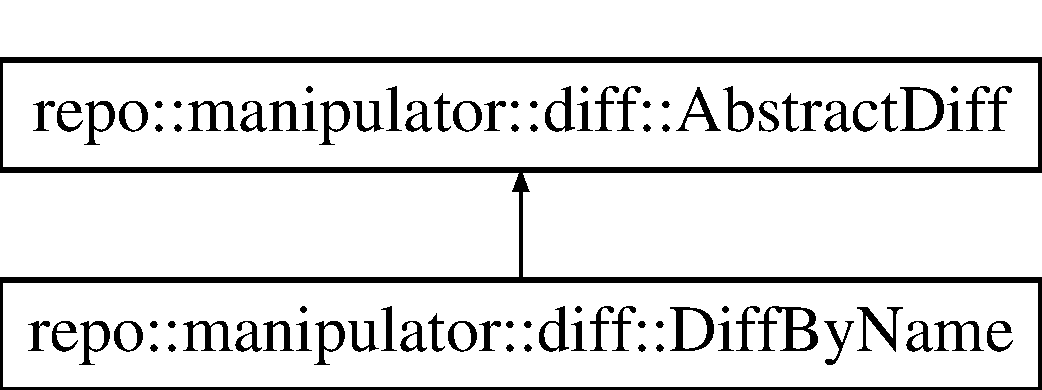
\includegraphics[height=2.000000cm]{classrepo_1_1manipulator_1_1diff_1_1_diff_by_name}
\end{center}
\end{figure}
\subsection*{Public Member Functions}
\begin{DoxyCompactItemize}
\item 
\hyperlink{classrepo_1_1manipulator_1_1diff_1_1_diff_by_name_a50225fea6e71da2d5f17dd023246920b}{Diff\+By\+Name} (const \hyperlink{classrepo_1_1core_1_1model_1_1_repo_scene}{repo\+::core\+::model\+::\+Repo\+Scene} $\ast$base, const \hyperlink{classrepo_1_1core_1_1model_1_1_repo_scene}{repo\+::core\+::model\+::\+Repo\+Scene} $\ast$compare, const \hyperlink{classrepo_1_1core_1_1model_1_1_repo_scene_aefcacd6eb4c7774ac1bfe3a6b223337c}{repo\+::core\+::model\+::\+Repo\+Scene\+::\+Graph\+Type} \&g\+Type=repo\+::core\+::model\+::\+Repo\+Scene\+::\+Graph\+Type\+::\+D\+E\+F\+A\+U\+L\+T)
\item 
virtual bool \hyperlink{classrepo_1_1manipulator_1_1diff_1_1_diff_by_name_a4cb80e41c9543f130903d83d43d78f98}{is\+Ok} (std\+::string \&msg) const 
\end{DoxyCompactItemize}
\subsection*{Additional Inherited Members}


\subsection{Constructor \& Destructor Documentation}
\hypertarget{classrepo_1_1manipulator_1_1diff_1_1_diff_by_name_a50225fea6e71da2d5f17dd023246920b}{}\index{repo\+::manipulator\+::diff\+::\+Diff\+By\+Name@{repo\+::manipulator\+::diff\+::\+Diff\+By\+Name}!Diff\+By\+Name@{Diff\+By\+Name}}
\index{Diff\+By\+Name@{Diff\+By\+Name}!repo\+::manipulator\+::diff\+::\+Diff\+By\+Name@{repo\+::manipulator\+::diff\+::\+Diff\+By\+Name}}
\subsubsection[{Diff\+By\+Name}]{\setlength{\rightskip}{0pt plus 5cm}Diff\+By\+Name\+::\+Diff\+By\+Name (
\begin{DoxyParamCaption}
\item[{const {\bf repo\+::core\+::model\+::\+Repo\+Scene} $\ast$}]{base, }
\item[{const {\bf repo\+::core\+::model\+::\+Repo\+Scene} $\ast$}]{compare, }
\item[{const {\bf repo\+::core\+::model\+::\+Repo\+Scene\+::\+Graph\+Type} \&}]{g\+Type = {\ttfamily repo\+:\+:core\+:\+:model\+:\+:RepoScene\+:\+:GraphType\+:\+:DEFAULT}}
\end{DoxyParamCaption}
)}\label{classrepo_1_1manipulator_1_1diff_1_1_diff_by_name_a50225fea6e71da2d5f17dd023246920b}
Construct a diff comparator given the 2 scenes supplied 
\begin{DoxyParams}{Parameters}
{\em base} & base scene to compare from \\
\hline
{\em compare} & scene to compare against \\
\hline
{\em g\+Type} & graph type to diff (default\+: unoptimised) \\
\hline
\end{DoxyParams}


\subsection{Member Function Documentation}
\hypertarget{classrepo_1_1manipulator_1_1diff_1_1_diff_by_name_a4cb80e41c9543f130903d83d43d78f98}{}\index{repo\+::manipulator\+::diff\+::\+Diff\+By\+Name@{repo\+::manipulator\+::diff\+::\+Diff\+By\+Name}!is\+Ok@{is\+Ok}}
\index{is\+Ok@{is\+Ok}!repo\+::manipulator\+::diff\+::\+Diff\+By\+Name@{repo\+::manipulator\+::diff\+::\+Diff\+By\+Name}}
\subsubsection[{is\+Ok}]{\setlength{\rightskip}{0pt plus 5cm}virtual bool repo\+::manipulator\+::diff\+::\+Diff\+By\+Name\+::is\+Ok (
\begin{DoxyParamCaption}
\item[{std\+::string \&}]{msg}
\end{DoxyParamCaption}
) const\hspace{0.3cm}{\ttfamily [inline]}, {\ttfamily [virtual]}}\label{classrepo_1_1manipulator_1_1diff_1_1_diff_by_name_a4cb80e41c9543f130903d83d43d78f98}
Check if comparator functioned fine 
\begin{DoxyParams}{Parameters}
{\em msg} & error message should boolean returns false \\
\hline
\end{DoxyParams}
\begin{DoxyReturn}{Returns}
returns true if comparator operated successfully 
\end{DoxyReturn}


Implements \hyperlink{classrepo_1_1manipulator_1_1diff_1_1_abstract_diff_a0c1780f099a434120e65835bd1514ebf}{repo\+::manipulator\+::diff\+::\+Abstract\+Diff}.



The documentation for this class was generated from the following files\+:\begin{DoxyCompactItemize}
\item 
C\+:/\+Users/\+Carmen/3\+D Repo/\+Repo/3drepobouncer/bouncer/src/repo/manipulator/diff/repo\+\_\+diff\+\_\+name.\+h\item 
C\+:/\+Users/\+Carmen/3\+D Repo/\+Repo/3drepobouncer/bouncer/src/repo/manipulator/diff/repo\+\_\+diff\+\_\+name.\+cpp\end{DoxyCompactItemize}

\hypertarget{classrepo_1_1manipulator_1_1diff_1_1_diff_by_shared_i_d}{}\section{repo\+:\+:manipulator\+:\+:diff\+:\+:Diff\+By\+Shared\+I\+D Class Reference}
\label{classrepo_1_1manipulator_1_1diff_1_1_diff_by_shared_i_d}\index{repo\+::manipulator\+::diff\+::\+Diff\+By\+Shared\+I\+D@{repo\+::manipulator\+::diff\+::\+Diff\+By\+Shared\+I\+D}}
Inheritance diagram for repo\+:\+:manipulator\+:\+:diff\+:\+:Diff\+By\+Shared\+I\+D\+:\begin{figure}[H]
\begin{center}
\leavevmode
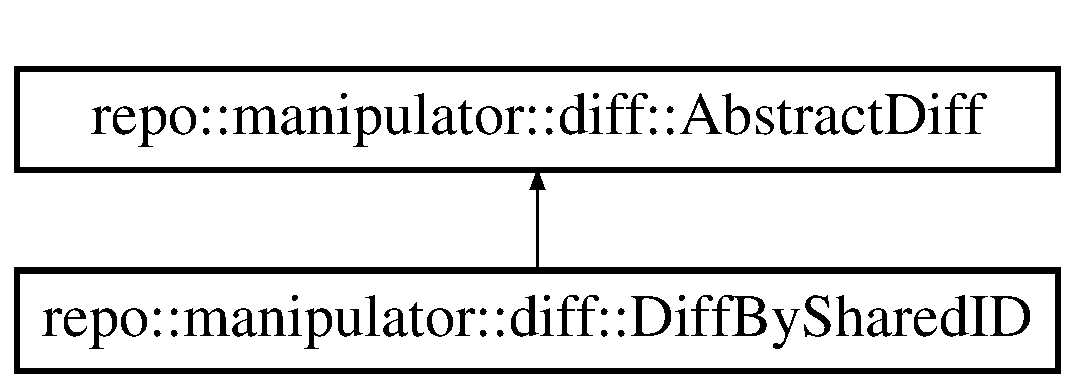
\includegraphics[height=2.000000cm]{classrepo_1_1manipulator_1_1diff_1_1_diff_by_shared_i_d}
\end{center}
\end{figure}
\subsection*{Public Member Functions}
\begin{DoxyCompactItemize}
\item 
\hyperlink{classrepo_1_1manipulator_1_1diff_1_1_diff_by_shared_i_d_a51a13c6d99b27dea1e338951712718b9}{Diff\+By\+Shared\+I\+D} (const \hyperlink{classrepo_1_1core_1_1model_1_1_repo_scene}{repo\+::core\+::model\+::\+Repo\+Scene} $\ast$base, const \hyperlink{classrepo_1_1core_1_1model_1_1_repo_scene}{repo\+::core\+::model\+::\+Repo\+Scene} $\ast$compare, const \hyperlink{classrepo_1_1core_1_1model_1_1_repo_scene_aefcacd6eb4c7774ac1bfe3a6b223337c}{repo\+::core\+::model\+::\+Repo\+Scene\+::\+Graph\+Type} \&g\+Type=repo\+::core\+::model\+::\+Repo\+Scene\+::\+Graph\+Type\+::\+D\+E\+F\+A\+U\+L\+T)
\item 
virtual bool \hyperlink{classrepo_1_1manipulator_1_1diff_1_1_diff_by_shared_i_d_afc3b71c3c85050b703c6ca3412c275e2}{is\+Ok} (std\+::string \&msg) const 
\end{DoxyCompactItemize}
\subsection*{Additional Inherited Members}


\subsection{Constructor \& Destructor Documentation}
\hypertarget{classrepo_1_1manipulator_1_1diff_1_1_diff_by_shared_i_d_a51a13c6d99b27dea1e338951712718b9}{}\index{repo\+::manipulator\+::diff\+::\+Diff\+By\+Shared\+I\+D@{repo\+::manipulator\+::diff\+::\+Diff\+By\+Shared\+I\+D}!Diff\+By\+Shared\+I\+D@{Diff\+By\+Shared\+I\+D}}
\index{Diff\+By\+Shared\+I\+D@{Diff\+By\+Shared\+I\+D}!repo\+::manipulator\+::diff\+::\+Diff\+By\+Shared\+I\+D@{repo\+::manipulator\+::diff\+::\+Diff\+By\+Shared\+I\+D}}
\subsubsection[{Diff\+By\+Shared\+I\+D}]{\setlength{\rightskip}{0pt plus 5cm}Diff\+By\+Shared\+I\+D\+::\+Diff\+By\+Shared\+I\+D (
\begin{DoxyParamCaption}
\item[{const {\bf repo\+::core\+::model\+::\+Repo\+Scene} $\ast$}]{base, }
\item[{const {\bf repo\+::core\+::model\+::\+Repo\+Scene} $\ast$}]{compare, }
\item[{const {\bf repo\+::core\+::model\+::\+Repo\+Scene\+::\+Graph\+Type} \&}]{g\+Type = {\ttfamily repo\+:\+:core\+:\+:model\+:\+:RepoScene\+:\+:GraphType\+:\+:DEFAULT}}
\end{DoxyParamCaption}
)}\label{classrepo_1_1manipulator_1_1diff_1_1_diff_by_shared_i_d_a51a13c6d99b27dea1e338951712718b9}
Construct a diff comparator given the 2 scenes supplied 
\begin{DoxyParams}{Parameters}
{\em base} & base scene to compare from \\
\hline
{\em compare} & scene to compare against \\
\hline
{\em g\+Type} & graph type to diff (default\+: unoptimised) \\
\hline
\end{DoxyParams}


\subsection{Member Function Documentation}
\hypertarget{classrepo_1_1manipulator_1_1diff_1_1_diff_by_shared_i_d_afc3b71c3c85050b703c6ca3412c275e2}{}\index{repo\+::manipulator\+::diff\+::\+Diff\+By\+Shared\+I\+D@{repo\+::manipulator\+::diff\+::\+Diff\+By\+Shared\+I\+D}!is\+Ok@{is\+Ok}}
\index{is\+Ok@{is\+Ok}!repo\+::manipulator\+::diff\+::\+Diff\+By\+Shared\+I\+D@{repo\+::manipulator\+::diff\+::\+Diff\+By\+Shared\+I\+D}}
\subsubsection[{is\+Ok}]{\setlength{\rightskip}{0pt plus 5cm}virtual bool repo\+::manipulator\+::diff\+::\+Diff\+By\+Shared\+I\+D\+::is\+Ok (
\begin{DoxyParamCaption}
\item[{std\+::string \&}]{msg}
\end{DoxyParamCaption}
) const\hspace{0.3cm}{\ttfamily [inline]}, {\ttfamily [virtual]}}\label{classrepo_1_1manipulator_1_1diff_1_1_diff_by_shared_i_d_afc3b71c3c85050b703c6ca3412c275e2}
Check if comparator functioned fine 
\begin{DoxyParams}{Parameters}
{\em msg} & error message should boolean returns false \\
\hline
\end{DoxyParams}
\begin{DoxyReturn}{Returns}
returns true if comparator operated successfully 
\end{DoxyReturn}


Implements \hyperlink{classrepo_1_1manipulator_1_1diff_1_1_abstract_diff_a0c1780f099a434120e65835bd1514ebf}{repo\+::manipulator\+::diff\+::\+Abstract\+Diff}.



The documentation for this class was generated from the following files\+:\begin{DoxyCompactItemize}
\item 
C\+:/\+Users/\+Carmen/3\+D Repo/\+Repo/3drepobouncer/bouncer/src/repo/manipulator/diff/repo\+\_\+diff\+\_\+sharedid.\+h\item 
C\+:/\+Users/\+Carmen/3\+D Repo/\+Repo/3drepobouncer/bouncer/src/repo/manipulator/diff/repo\+\_\+diff\+\_\+sharedid.\+cpp\end{DoxyCompactItemize}

\hypertarget{classrepo_1_1manipulator_1_1modelconvertor_1_1_g_l_t_f_model_export}{}\section{repo\+:\+:manipulator\+:\+:modelconvertor\+:\+:G\+L\+T\+F\+Model\+Export Class Reference}
\label{classrepo_1_1manipulator_1_1modelconvertor_1_1_g_l_t_f_model_export}\index{repo\+::manipulator\+::modelconvertor\+::\+G\+L\+T\+F\+Model\+Export@{repo\+::manipulator\+::modelconvertor\+::\+G\+L\+T\+F\+Model\+Export}}
Inheritance diagram for repo\+:\+:manipulator\+:\+:modelconvertor\+:\+:G\+L\+T\+F\+Model\+Export\+:\begin{figure}[H]
\begin{center}
\leavevmode
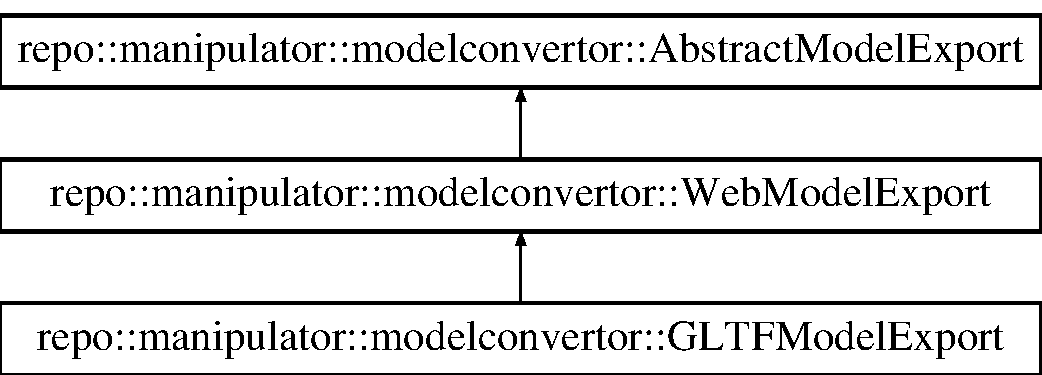
\includegraphics[height=3.000000cm]{classrepo_1_1manipulator_1_1modelconvertor_1_1_g_l_t_f_model_export}
\end{center}
\end{figure}
\subsection*{Public Member Functions}
\begin{DoxyCompactItemize}
\item 
\hyperlink{classrepo_1_1manipulator_1_1modelconvertor_1_1_g_l_t_f_model_export_a11dfb0019a718133d1848f273b44aa09}{G\+L\+T\+F\+Model\+Export} (const \hyperlink{classrepo_1_1core_1_1model_1_1_repo_scene}{repo\+::core\+::model\+::\+Repo\+Scene} $\ast$scene)
\item 
virtual \hyperlink{classrepo_1_1manipulator_1_1modelconvertor_1_1_g_l_t_f_model_export_a1c641b8c048ce68454409e5b6cb232e9}{$\sim$\+G\+L\+T\+F\+Model\+Export} ()
\item 
\hyperlink{structrepo__web__buffers__t}{repo\+\_\+web\+\_\+buffers\+\_\+t} \hyperlink{classrepo_1_1manipulator_1_1modelconvertor_1_1_g_l_t_f_model_export_af46ede52b996784ab8b7ff15977d186d}{get\+All\+Files\+Exported\+As\+Buffer} () const 
\end{DoxyCompactItemize}
\subsection*{Additional Inherited Members}


\subsection{Constructor \& Destructor Documentation}
\hypertarget{classrepo_1_1manipulator_1_1modelconvertor_1_1_g_l_t_f_model_export_a11dfb0019a718133d1848f273b44aa09}{}\index{repo\+::manipulator\+::modelconvertor\+::\+G\+L\+T\+F\+Model\+Export@{repo\+::manipulator\+::modelconvertor\+::\+G\+L\+T\+F\+Model\+Export}!G\+L\+T\+F\+Model\+Export@{G\+L\+T\+F\+Model\+Export}}
\index{G\+L\+T\+F\+Model\+Export@{G\+L\+T\+F\+Model\+Export}!repo\+::manipulator\+::modelconvertor\+::\+G\+L\+T\+F\+Model\+Export@{repo\+::manipulator\+::modelconvertor\+::\+G\+L\+T\+F\+Model\+Export}}
\subsubsection[{G\+L\+T\+F\+Model\+Export}]{\setlength{\rightskip}{0pt plus 5cm}G\+L\+T\+F\+Model\+Export\+::\+G\+L\+T\+F\+Model\+Export (
\begin{DoxyParamCaption}
\item[{const {\bf repo\+::core\+::model\+::\+Repo\+Scene} $\ast$}]{scene}
\end{DoxyParamCaption}
)}\label{classrepo_1_1manipulator_1_1modelconvertor_1_1_g_l_t_f_model_export_a11dfb0019a718133d1848f273b44aa09}
Default Constructor, export model with default settings 
\begin{DoxyParams}{Parameters}
{\em scene} & repo scene to convert \\
\hline
\end{DoxyParams}
\hypertarget{classrepo_1_1manipulator_1_1modelconvertor_1_1_g_l_t_f_model_export_a1c641b8c048ce68454409e5b6cb232e9}{}\index{repo\+::manipulator\+::modelconvertor\+::\+G\+L\+T\+F\+Model\+Export@{repo\+::manipulator\+::modelconvertor\+::\+G\+L\+T\+F\+Model\+Export}!````~G\+L\+T\+F\+Model\+Export@{$\sim$\+G\+L\+T\+F\+Model\+Export}}
\index{````~G\+L\+T\+F\+Model\+Export@{$\sim$\+G\+L\+T\+F\+Model\+Export}!repo\+::manipulator\+::modelconvertor\+::\+G\+L\+T\+F\+Model\+Export@{repo\+::manipulator\+::modelconvertor\+::\+G\+L\+T\+F\+Model\+Export}}
\subsubsection[{$\sim$\+G\+L\+T\+F\+Model\+Export}]{\setlength{\rightskip}{0pt plus 5cm}G\+L\+T\+F\+Model\+Export\+::$\sim$\+G\+L\+T\+F\+Model\+Export (
\begin{DoxyParamCaption}
{}
\end{DoxyParamCaption}
)\hspace{0.3cm}{\ttfamily [virtual]}}\label{classrepo_1_1manipulator_1_1modelconvertor_1_1_g_l_t_f_model_export_a1c641b8c048ce68454409e5b6cb232e9}
Default Destructor 

\subsection{Member Function Documentation}
\hypertarget{classrepo_1_1manipulator_1_1modelconvertor_1_1_g_l_t_f_model_export_af46ede52b996784ab8b7ff15977d186d}{}\index{repo\+::manipulator\+::modelconvertor\+::\+G\+L\+T\+F\+Model\+Export@{repo\+::manipulator\+::modelconvertor\+::\+G\+L\+T\+F\+Model\+Export}!get\+All\+Files\+Exported\+As\+Buffer@{get\+All\+Files\+Exported\+As\+Buffer}}
\index{get\+All\+Files\+Exported\+As\+Buffer@{get\+All\+Files\+Exported\+As\+Buffer}!repo\+::manipulator\+::modelconvertor\+::\+G\+L\+T\+F\+Model\+Export@{repo\+::manipulator\+::modelconvertor\+::\+G\+L\+T\+F\+Model\+Export}}
\subsubsection[{get\+All\+Files\+Exported\+As\+Buffer}]{\setlength{\rightskip}{0pt plus 5cm}{\bf repo\+\_\+web\+\_\+buffers\+\_\+t} G\+L\+T\+F\+Model\+Export\+::get\+All\+Files\+Exported\+As\+Buffer (
\begin{DoxyParamCaption}
{}
\end{DoxyParamCaption}
) const\hspace{0.3cm}{\ttfamily [virtual]}}\label{classrepo_1_1manipulator_1_1modelconvertor_1_1_g_l_t_f_model_export_af46ede52b996784ab8b7ff15977d186d}
Export all necessary files as buffers \begin{DoxyReturn}{Returns}
returns a repo\+\_\+src\+\_\+export\+\_\+t containing all files needed for this model to be rendered 
\end{DoxyReturn}


Implements \hyperlink{classrepo_1_1manipulator_1_1modelconvertor_1_1_web_model_export_ad9e20343a2e8a21fb9de2e89ba14bf05}{repo\+::manipulator\+::modelconvertor\+::\+Web\+Model\+Export}.



The documentation for this class was generated from the following files\+:\begin{DoxyCompactItemize}
\item 
C\+:/\+Users/\+Carmen/3\+D Repo/\+Repo/3drepobouncer/bouncer/src/repo/manipulator/modelconvertor/export/repo\+\_\+model\+\_\+export\+\_\+gltf.\+h\item 
C\+:/\+Users/\+Carmen/3\+D Repo/\+Repo/3drepobouncer/bouncer/src/repo/manipulator/modelconvertor/export/repo\+\_\+model\+\_\+export\+\_\+gltf.\+cpp\end{DoxyCompactItemize}

\hypertarget{classrepo_1_1manipulator_1_1modeloptimizer_1_1_i_f_c_optimzer}{}\section{repo\+:\+:manipulator\+:\+:modeloptimizer\+:\+:I\+F\+C\+Optimzer Class Reference}
\label{classrepo_1_1manipulator_1_1modeloptimizer_1_1_i_f_c_optimzer}\index{repo\+::manipulator\+::modeloptimizer\+::\+I\+F\+C\+Optimzer@{repo\+::manipulator\+::modeloptimizer\+::\+I\+F\+C\+Optimzer}}
Inheritance diagram for repo\+:\+:manipulator\+:\+:modeloptimizer\+:\+:I\+F\+C\+Optimzer\+:\begin{figure}[H]
\begin{center}
\leavevmode
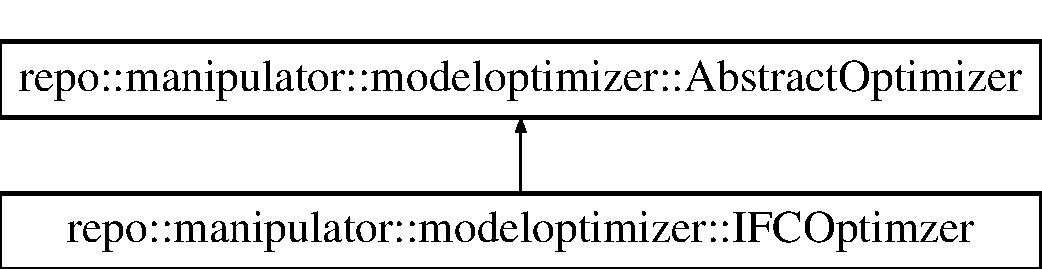
\includegraphics[height=2.000000cm]{classrepo_1_1manipulator_1_1modeloptimizer_1_1_i_f_c_optimzer}
\end{center}
\end{figure}
\subsection*{Public Member Functions}
\begin{DoxyCompactItemize}
\item 
\hyperlink{classrepo_1_1manipulator_1_1modeloptimizer_1_1_i_f_c_optimzer_a8ee34a88f9103142aa677279264773e8}{I\+F\+C\+Optimzer} ()
\item 
virtual \hyperlink{classrepo_1_1manipulator_1_1modeloptimizer_1_1_i_f_c_optimzer_ad12a91fe9357bda07592df46b549671a}{$\sim$\+I\+F\+C\+Optimzer} ()
\item 
virtual bool \hyperlink{classrepo_1_1manipulator_1_1modeloptimizer_1_1_i_f_c_optimzer_a5ea4e1e6cd502d72a3ba3cca593eb9d3}{apply} (\hyperlink{classrepo_1_1core_1_1model_1_1_repo_scene}{repo\+::core\+::model\+::\+Repo\+Scene} $\ast$scene)
\end{DoxyCompactItemize}


\subsection{Constructor \& Destructor Documentation}
\hypertarget{classrepo_1_1manipulator_1_1modeloptimizer_1_1_i_f_c_optimzer_a8ee34a88f9103142aa677279264773e8}{}\index{repo\+::manipulator\+::modeloptimizer\+::\+I\+F\+C\+Optimzer@{repo\+::manipulator\+::modeloptimizer\+::\+I\+F\+C\+Optimzer}!I\+F\+C\+Optimzer@{I\+F\+C\+Optimzer}}
\index{I\+F\+C\+Optimzer@{I\+F\+C\+Optimzer}!repo\+::manipulator\+::modeloptimizer\+::\+I\+F\+C\+Optimzer@{repo\+::manipulator\+::modeloptimizer\+::\+I\+F\+C\+Optimzer}}
\subsubsection[{I\+F\+C\+Optimzer}]{\setlength{\rightskip}{0pt plus 5cm}I\+F\+C\+Optimzer\+::\+I\+F\+C\+Optimzer (
\begin{DoxyParamCaption}
{}
\end{DoxyParamCaption}
)}\label{classrepo_1_1manipulator_1_1modeloptimizer_1_1_i_f_c_optimzer_a8ee34a88f9103142aa677279264773e8}
Default constructor \hypertarget{classrepo_1_1manipulator_1_1modeloptimizer_1_1_i_f_c_optimzer_ad12a91fe9357bda07592df46b549671a}{}\index{repo\+::manipulator\+::modeloptimizer\+::\+I\+F\+C\+Optimzer@{repo\+::manipulator\+::modeloptimizer\+::\+I\+F\+C\+Optimzer}!````~I\+F\+C\+Optimzer@{$\sim$\+I\+F\+C\+Optimzer}}
\index{````~I\+F\+C\+Optimzer@{$\sim$\+I\+F\+C\+Optimzer}!repo\+::manipulator\+::modeloptimizer\+::\+I\+F\+C\+Optimzer@{repo\+::manipulator\+::modeloptimizer\+::\+I\+F\+C\+Optimzer}}
\subsubsection[{$\sim$\+I\+F\+C\+Optimzer}]{\setlength{\rightskip}{0pt plus 5cm}I\+F\+C\+Optimzer\+::$\sim$\+I\+F\+C\+Optimzer (
\begin{DoxyParamCaption}
{}
\end{DoxyParamCaption}
)\hspace{0.3cm}{\ttfamily [virtual]}}\label{classrepo_1_1manipulator_1_1modeloptimizer_1_1_i_f_c_optimzer_ad12a91fe9357bda07592df46b549671a}
Default deconstructor 

\subsection{Member Function Documentation}
\hypertarget{classrepo_1_1manipulator_1_1modeloptimizer_1_1_i_f_c_optimzer_a5ea4e1e6cd502d72a3ba3cca593eb9d3}{}\index{repo\+::manipulator\+::modeloptimizer\+::\+I\+F\+C\+Optimzer@{repo\+::manipulator\+::modeloptimizer\+::\+I\+F\+C\+Optimzer}!apply@{apply}}
\index{apply@{apply}!repo\+::manipulator\+::modeloptimizer\+::\+I\+F\+C\+Optimzer@{repo\+::manipulator\+::modeloptimizer\+::\+I\+F\+C\+Optimzer}}
\subsubsection[{apply}]{\setlength{\rightskip}{0pt plus 5cm}bool I\+F\+C\+Optimzer\+::apply (
\begin{DoxyParamCaption}
\item[{{\bf repo\+::core\+::model\+::\+Repo\+Scene} $\ast$}]{scene}
\end{DoxyParamCaption}
)\hspace{0.3cm}{\ttfamily [virtual]}}\label{classrepo_1_1manipulator_1_1modeloptimizer_1_1_i_f_c_optimzer_a5ea4e1e6cd502d72a3ba3cca593eb9d3}
Apply optimisation on the given repo\+Scene 
\begin{DoxyParams}{Parameters}
{\em scene} & takes in a repo\+Scene to optimise \\
\hline
\end{DoxyParams}
\begin{DoxyReturn}{Returns}
returns true upon success 
\end{DoxyReturn}


Implements \hyperlink{classrepo_1_1manipulator_1_1modeloptimizer_1_1_abstract_optimizer_a38e98344c1d3c66fbea8adae41dc6cb1}{repo\+::manipulator\+::modeloptimizer\+::\+Abstract\+Optimizer}.



The documentation for this class was generated from the following files\+:\begin{DoxyCompactItemize}
\item 
C\+:/\+Users/\+Carmen/3\+D Repo/\+Repo/3drepobouncer/bouncer/src/repo/manipulator/modeloptimizer/repo\+\_\+optimizer\+\_\+ifc.\+h\item 
C\+:/\+Users/\+Carmen/3\+D Repo/\+Repo/3drepobouncer/bouncer/src/repo/manipulator/modeloptimizer/repo\+\_\+optimizer\+\_\+ifc.\+cpp\end{DoxyCompactItemize}

\hypertarget{classrepo_1_1lib_1_1_log_to_stdout}{}\section{repo\+:\+:lib\+:\+:Log\+To\+Stdout Class Reference}
\label{classrepo_1_1lib_1_1_log_to_stdout}\index{repo\+::lib\+::\+Log\+To\+Stdout@{repo\+::lib\+::\+Log\+To\+Stdout}}
Inheritance diagram for repo\+:\+:lib\+:\+:Log\+To\+Stdout\+:\begin{figure}[H]
\begin{center}
\leavevmode
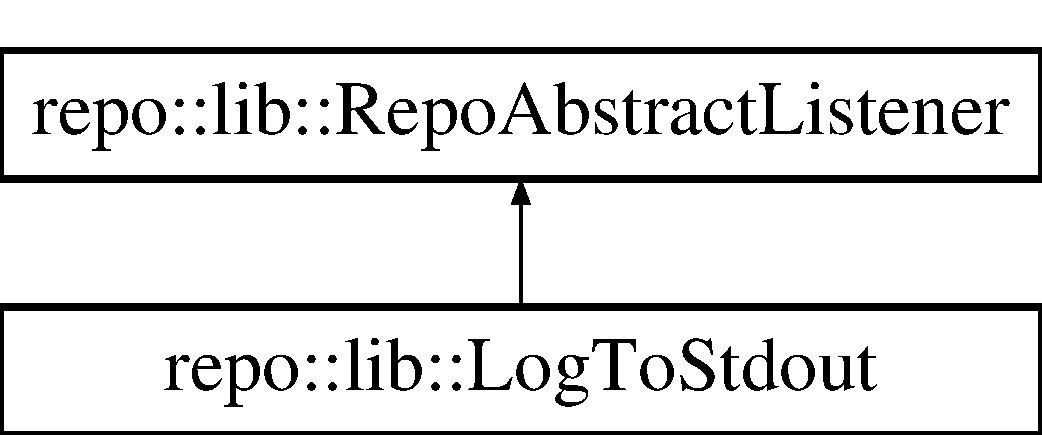
\includegraphics[height=2.000000cm]{classrepo_1_1lib_1_1_log_to_stdout}
\end{center}
\end{figure}
\subsection*{Public Member Functions}
\begin{DoxyCompactItemize}
\item 
\hypertarget{classrepo_1_1lib_1_1_log_to_stdout_a85acbe84f9dd35f2ccf91a314733685f}{}virtual void {\bfseries message\+Generated} (const std\+::string \&message)\label{classrepo_1_1lib_1_1_log_to_stdout_a85acbe84f9dd35f2ccf91a314733685f}

\end{DoxyCompactItemize}


The documentation for this class was generated from the following file\+:\begin{DoxyCompactItemize}
\item 
C\+:/\+Users/\+Carmen/3\+D Repo/\+Repo/3drepobouncer/bouncer/src/repo/lib/repo\+\_\+listener\+\_\+stdout.\+h\end{DoxyCompactItemize}

\hypertarget{classrepo_1_1core_1_1model_1_1_map_node}{}\section{repo\+:\+:core\+:\+:model\+:\+:Map\+Node Class Reference}
\label{classrepo_1_1core_1_1model_1_1_map_node}\index{repo\+::core\+::model\+::\+Map\+Node@{repo\+::core\+::model\+::\+Map\+Node}}
Inheritance diagram for repo\+:\+:core\+:\+:model\+:\+:Map\+Node\+:\begin{figure}[H]
\begin{center}
\leavevmode
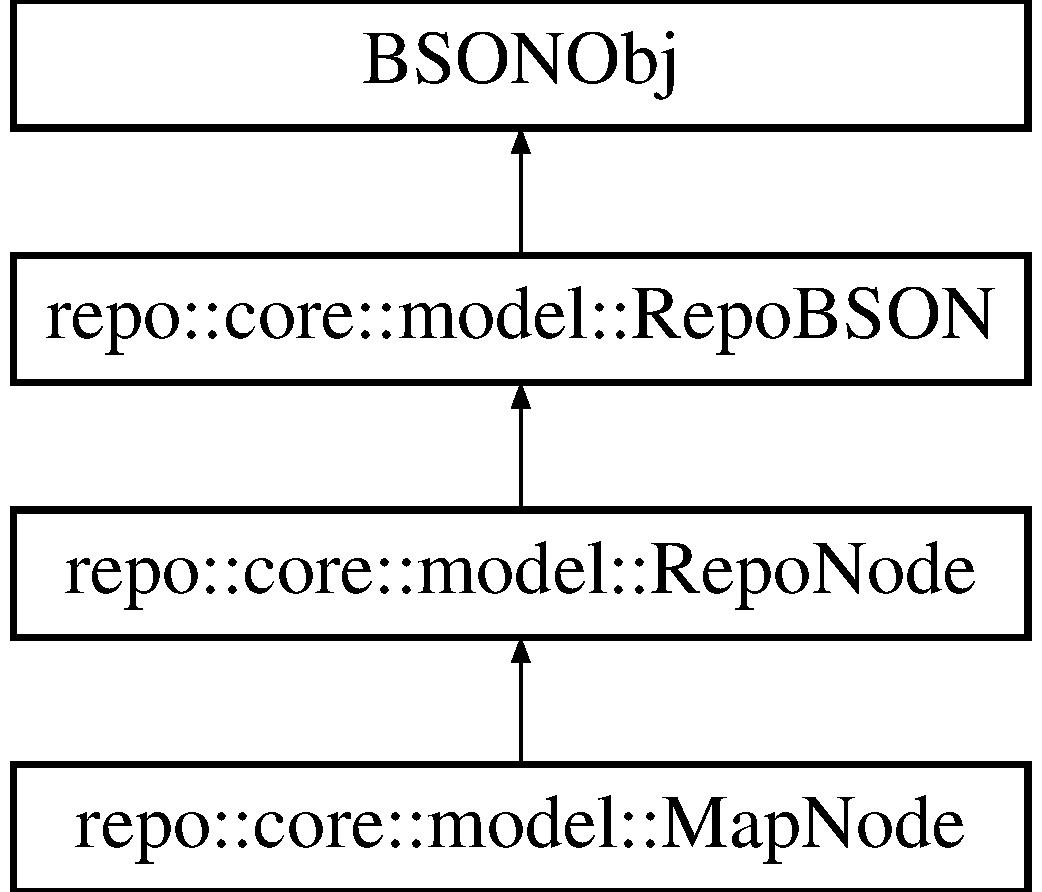
\includegraphics[height=4.000000cm]{classrepo_1_1core_1_1model_1_1_map_node}
\end{center}
\end{figure}
\subsection*{Public Member Functions}
\begin{DoxyCompactItemize}
\item 
\hyperlink{classrepo_1_1core_1_1model_1_1_map_node_aa4e1fb66b032e08781093ffb7fe03885}{Map\+Node} ()
\item 
\hyperlink{classrepo_1_1core_1_1model_1_1_map_node_a44379bbf090c4ed529c892a6c3482e58}{Map\+Node} (\hyperlink{classrepo_1_1core_1_1model_1_1_repo_b_s_o_n}{Repo\+B\+S\+O\+N} bson)
\item 
\hyperlink{classrepo_1_1core_1_1model_1_1_map_node_a380098b662362882a2d5ca3bd5004fc1}{$\sim$\+Map\+Node} ()
\item 
std\+::string \hyperlink{classrepo_1_1core_1_1model_1_1_map_node_ab17c7f35002dccd86a8d0a0aa137fb29}{get\+A\+P\+I\+Key} () const 
\item 
\hypertarget{classrepo_1_1core_1_1model_1_1_map_node_aa18ba0dc0bf85a2ef4e7499ffbff445c}{}\hyperlink{structrepo__vector__t}{repo\+\_\+vector\+\_\+t} {\bfseries get\+Centre} () const \label{classrepo_1_1core_1_1model_1_1_map_node_aa18ba0dc0bf85a2ef4e7499ffbff445c}

\item 
bool \hyperlink{classrepo_1_1core_1_1model_1_1_map_node_a51180c085b8dc221c57542dcace32b51}{is\+Two\+Sided} () const 
\item 
float \hyperlink{classrepo_1_1core_1_1model_1_1_map_node_a009d9786e3760f21af80bc4b40d12d8a}{get\+Two\+Sided\+Value} () const 
\item 
std\+::string \hyperlink{classrepo_1_1core_1_1model_1_1_map_node_a5a600efde8d866325a144e90b0a0d2c9}{get\+Map\+Type} () const 
\item 
float \hyperlink{classrepo_1_1core_1_1model_1_1_map_node_a1a3b603981a4b51cb69b1b83b793e849}{get\+Lat} () const 
\item 
float \hyperlink{classrepo_1_1core_1_1model_1_1_map_node_a7600f38ebfdffdb89db77f3ea8aa3ca6}{get\+Long} () const 
\item 
float \hyperlink{classrepo_1_1core_1_1model_1_1_map_node_ac9925b3ed29f02187501717e34b564c0}{get\+Tile\+Size} () const 
\item 
uint32\+\_\+t \hyperlink{classrepo_1_1core_1_1model_1_1_map_node_a841b65e0ae5039e638d79d92f4ba01c1}{get\+Width} () const 
\item 
float \hyperlink{classrepo_1_1core_1_1model_1_1_map_node_a10614a78ca490a541b3704214e1ec5cb}{get\+Y\+Rot} () const 
\item 
uint32\+\_\+t \hyperlink{classrepo_1_1core_1_1model_1_1_map_node_aa5409677aba6f413c335d26216fa40d7}{get\+Zoom} () const 
\item 
virtual bool \hyperlink{classrepo_1_1core_1_1model_1_1_map_node_ac27593deef8281f9d70324f2f1f994e9}{s\+Equal} (const \hyperlink{classrepo_1_1core_1_1model_1_1_repo_node}{Repo\+Node} \&other) const 
\end{DoxyCompactItemize}
\subsection*{Additional Inherited Members}


\subsection{Constructor \& Destructor Documentation}
\hypertarget{classrepo_1_1core_1_1model_1_1_map_node_aa4e1fb66b032e08781093ffb7fe03885}{}\index{repo\+::core\+::model\+::\+Map\+Node@{repo\+::core\+::model\+::\+Map\+Node}!Map\+Node@{Map\+Node}}
\index{Map\+Node@{Map\+Node}!repo\+::core\+::model\+::\+Map\+Node@{repo\+::core\+::model\+::\+Map\+Node}}
\subsubsection[{Map\+Node}]{\setlength{\rightskip}{0pt plus 5cm}Map\+Node\+::\+Map\+Node (
\begin{DoxyParamCaption}
{}
\end{DoxyParamCaption}
)}\label{classrepo_1_1core_1_1model_1_1_map_node_aa4e1fb66b032e08781093ffb7fe03885}
Default constructor \hypertarget{classrepo_1_1core_1_1model_1_1_map_node_a44379bbf090c4ed529c892a6c3482e58}{}\index{repo\+::core\+::model\+::\+Map\+Node@{repo\+::core\+::model\+::\+Map\+Node}!Map\+Node@{Map\+Node}}
\index{Map\+Node@{Map\+Node}!repo\+::core\+::model\+::\+Map\+Node@{repo\+::core\+::model\+::\+Map\+Node}}
\subsubsection[{Map\+Node}]{\setlength{\rightskip}{0pt plus 5cm}Map\+Node\+::\+Map\+Node (
\begin{DoxyParamCaption}
\item[{{\bf Repo\+B\+S\+O\+N}}]{bson}
\end{DoxyParamCaption}
)}\label{classrepo_1_1core_1_1model_1_1_map_node_a44379bbf090c4ed529c892a6c3482e58}
Construct a \hyperlink{classrepo_1_1core_1_1model_1_1_map_node}{Map\+Node} from a \hyperlink{classrepo_1_1core_1_1model_1_1_repo_b_s_o_n}{Repo\+B\+S\+O\+N} object 
\begin{DoxyParams}{Parameters}
{\em \hyperlink{classrepo_1_1core_1_1model_1_1_repo_b_s_o_n}{Repo\+B\+S\+O\+N}} & object \\
\hline
\end{DoxyParams}
\hypertarget{classrepo_1_1core_1_1model_1_1_map_node_a380098b662362882a2d5ca3bd5004fc1}{}\index{repo\+::core\+::model\+::\+Map\+Node@{repo\+::core\+::model\+::\+Map\+Node}!````~Map\+Node@{$\sim$\+Map\+Node}}
\index{````~Map\+Node@{$\sim$\+Map\+Node}!repo\+::core\+::model\+::\+Map\+Node@{repo\+::core\+::model\+::\+Map\+Node}}
\subsubsection[{$\sim$\+Map\+Node}]{\setlength{\rightskip}{0pt plus 5cm}Map\+Node\+::$\sim$\+Map\+Node (
\begin{DoxyParamCaption}
{}
\end{DoxyParamCaption}
)}\label{classrepo_1_1core_1_1model_1_1_map_node_a380098b662362882a2d5ca3bd5004fc1}
Default deconstructor 

\subsection{Member Function Documentation}
\hypertarget{classrepo_1_1core_1_1model_1_1_map_node_ab17c7f35002dccd86a8d0a0aa137fb29}{}\index{repo\+::core\+::model\+::\+Map\+Node@{repo\+::core\+::model\+::\+Map\+Node}!get\+A\+P\+I\+Key@{get\+A\+P\+I\+Key}}
\index{get\+A\+P\+I\+Key@{get\+A\+P\+I\+Key}!repo\+::core\+::model\+::\+Map\+Node@{repo\+::core\+::model\+::\+Map\+Node}}
\subsubsection[{get\+A\+P\+I\+Key}]{\setlength{\rightskip}{0pt plus 5cm}std\+::string repo\+::core\+::model\+::\+Map\+Node\+::get\+A\+P\+I\+Key (
\begin{DoxyParamCaption}
{}
\end{DoxyParamCaption}
) const\hspace{0.3cm}{\ttfamily [inline]}}\label{classrepo_1_1core_1_1model_1_1_map_node_ab17c7f35002dccd86a8d0a0aa137fb29}
-\/-\/-\/-\/-\/-\/--- Convenience functions -\/-\/-\/-\/-\/-\/-\/-\/--- \hypertarget{classrepo_1_1core_1_1model_1_1_map_node_a1a3b603981a4b51cb69b1b83b793e849}{}\index{repo\+::core\+::model\+::\+Map\+Node@{repo\+::core\+::model\+::\+Map\+Node}!get\+Lat@{get\+Lat}}
\index{get\+Lat@{get\+Lat}!repo\+::core\+::model\+::\+Map\+Node@{repo\+::core\+::model\+::\+Map\+Node}}
\subsubsection[{get\+Lat}]{\setlength{\rightskip}{0pt plus 5cm}float Map\+Node\+::get\+Lat (
\begin{DoxyParamCaption}
{}
\end{DoxyParamCaption}
) const}\label{classrepo_1_1core_1_1model_1_1_map_node_a1a3b603981a4b51cb69b1b83b793e849}
Get the Latitude value from the map  returns Latitude value, 0 \hypertarget{classrepo_1_1core_1_1model_1_1_map_node_a7600f38ebfdffdb89db77f3ea8aa3ca6}{}\index{repo\+::core\+::model\+::\+Map\+Node@{repo\+::core\+::model\+::\+Map\+Node}!get\+Long@{get\+Long}}
\index{get\+Long@{get\+Long}!repo\+::core\+::model\+::\+Map\+Node@{repo\+::core\+::model\+::\+Map\+Node}}
\subsubsection[{get\+Long}]{\setlength{\rightskip}{0pt plus 5cm}float Map\+Node\+::get\+Long (
\begin{DoxyParamCaption}
{}
\end{DoxyParamCaption}
) const}\label{classrepo_1_1core_1_1model_1_1_map_node_a7600f38ebfdffdb89db77f3ea8aa3ca6}
Get the Longitude value from the map  returns Longitude value, 0 \hypertarget{classrepo_1_1core_1_1model_1_1_map_node_a5a600efde8d866325a144e90b0a0d2c9}{}\index{repo\+::core\+::model\+::\+Map\+Node@{repo\+::core\+::model\+::\+Map\+Node}!get\+Map\+Type@{get\+Map\+Type}}
\index{get\+Map\+Type@{get\+Map\+Type}!repo\+::core\+::model\+::\+Map\+Node@{repo\+::core\+::model\+::\+Map\+Node}}
\subsubsection[{get\+Map\+Type}]{\setlength{\rightskip}{0pt plus 5cm}std\+::string repo\+::core\+::model\+::\+Map\+Node\+::get\+Map\+Type (
\begin{DoxyParamCaption}
{}
\end{DoxyParamCaption}
) const\hspace{0.3cm}{\ttfamily [inline]}}\label{classrepo_1_1core_1_1model_1_1_map_node_a5a600efde8d866325a144e90b0a0d2c9}
Get the type of map \begin{DoxyReturn}{Returns}
returns type of map as a string, empty string if not found 
\end{DoxyReturn}
\hypertarget{classrepo_1_1core_1_1model_1_1_map_node_ac9925b3ed29f02187501717e34b564c0}{}\index{repo\+::core\+::model\+::\+Map\+Node@{repo\+::core\+::model\+::\+Map\+Node}!get\+Tile\+Size@{get\+Tile\+Size}}
\index{get\+Tile\+Size@{get\+Tile\+Size}!repo\+::core\+::model\+::\+Map\+Node@{repo\+::core\+::model\+::\+Map\+Node}}
\subsubsection[{get\+Tile\+Size}]{\setlength{\rightskip}{0pt plus 5cm}float Map\+Node\+::get\+Tile\+Size (
\begin{DoxyParamCaption}
{}
\end{DoxyParamCaption}
) const}\label{classrepo_1_1core_1_1model_1_1_map_node_ac9925b3ed29f02187501717e34b564c0}
Get world tile size from map  returns world tile size, 1 if not found \hypertarget{classrepo_1_1core_1_1model_1_1_map_node_a009d9786e3760f21af80bc4b40d12d8a}{}\index{repo\+::core\+::model\+::\+Map\+Node@{repo\+::core\+::model\+::\+Map\+Node}!get\+Two\+Sided\+Value@{get\+Two\+Sided\+Value}}
\index{get\+Two\+Sided\+Value@{get\+Two\+Sided\+Value}!repo\+::core\+::model\+::\+Map\+Node@{repo\+::core\+::model\+::\+Map\+Node}}
\subsubsection[{get\+Two\+Sided\+Value}]{\setlength{\rightskip}{0pt plus 5cm}float repo\+::core\+::model\+::\+Map\+Node\+::get\+Two\+Sided\+Value (
\begin{DoxyParamCaption}
{}
\end{DoxyParamCaption}
) const\hspace{0.3cm}{\ttfamily [inline]}}\label{classrepo_1_1core_1_1model_1_1_map_node_a009d9786e3760f21af80bc4b40d12d8a}
Get the alpha value if the map tiles are 2 sided This is meaningless if \hyperlink{classrepo_1_1core_1_1model_1_1_map_node_a51180c085b8dc221c57542dcace32b51}{is\+Two\+Sided()} returned false Only call this function if is\+Two\+Sided is true \begin{DoxyReturn}{Returns}
returns the alpha value for the two sided tiles 
\end{DoxyReturn}
\hypertarget{classrepo_1_1core_1_1model_1_1_map_node_a841b65e0ae5039e638d79d92f4ba01c1}{}\index{repo\+::core\+::model\+::\+Map\+Node@{repo\+::core\+::model\+::\+Map\+Node}!get\+Width@{get\+Width}}
\index{get\+Width@{get\+Width}!repo\+::core\+::model\+::\+Map\+Node@{repo\+::core\+::model\+::\+Map\+Node}}
\subsubsection[{get\+Width}]{\setlength{\rightskip}{0pt plus 5cm}uint32\+\_\+t Map\+Node\+::get\+Width (
\begin{DoxyParamCaption}
{}
\end{DoxyParamCaption}
) const}\label{classrepo_1_1core_1_1model_1_1_map_node_a841b65e0ae5039e638d79d92f4ba01c1}
Get the tile width \begin{DoxyReturn}{Returns}
returns the tile width 
\end{DoxyReturn}
\hypertarget{classrepo_1_1core_1_1model_1_1_map_node_a10614a78ca490a541b3704214e1ec5cb}{}\index{repo\+::core\+::model\+::\+Map\+Node@{repo\+::core\+::model\+::\+Map\+Node}!get\+Y\+Rot@{get\+Y\+Rot}}
\index{get\+Y\+Rot@{get\+Y\+Rot}!repo\+::core\+::model\+::\+Map\+Node@{repo\+::core\+::model\+::\+Map\+Node}}
\subsubsection[{get\+Y\+Rot}]{\setlength{\rightskip}{0pt plus 5cm}float Map\+Node\+::get\+Y\+Rot (
\begin{DoxyParamCaption}
{}
\end{DoxyParamCaption}
) const}\label{classrepo_1_1core_1_1model_1_1_map_node_a10614a78ca490a541b3704214e1ec5cb}
Get Y Rotational(tilt) from the map  returns the rotational tilt \hypertarget{classrepo_1_1core_1_1model_1_1_map_node_aa5409677aba6f413c335d26216fa40d7}{}\index{repo\+::core\+::model\+::\+Map\+Node@{repo\+::core\+::model\+::\+Map\+Node}!get\+Zoom@{get\+Zoom}}
\index{get\+Zoom@{get\+Zoom}!repo\+::core\+::model\+::\+Map\+Node@{repo\+::core\+::model\+::\+Map\+Node}}
\subsubsection[{get\+Zoom}]{\setlength{\rightskip}{0pt plus 5cm}uint32\+\_\+t Map\+Node\+::get\+Zoom (
\begin{DoxyParamCaption}
{}
\end{DoxyParamCaption}
) const}\label{classrepo_1_1core_1_1model_1_1_map_node_aa5409677aba6f413c335d26216fa40d7}
Get zoom value \begin{DoxyReturn}{Returns}
returns zoom value, 0 if not found 
\end{DoxyReturn}
\hypertarget{classrepo_1_1core_1_1model_1_1_map_node_a51180c085b8dc221c57542dcace32b51}{}\index{repo\+::core\+::model\+::\+Map\+Node@{repo\+::core\+::model\+::\+Map\+Node}!is\+Two\+Sided@{is\+Two\+Sided}}
\index{is\+Two\+Sided@{is\+Two\+Sided}!repo\+::core\+::model\+::\+Map\+Node@{repo\+::core\+::model\+::\+Map\+Node}}
\subsubsection[{is\+Two\+Sided}]{\setlength{\rightskip}{0pt plus 5cm}bool repo\+::core\+::model\+::\+Map\+Node\+::is\+Two\+Sided (
\begin{DoxyParamCaption}
{}
\end{DoxyParamCaption}
) const\hspace{0.3cm}{\ttfamily [inline]}}\label{classrepo_1_1core_1_1model_1_1_map_node_a51180c085b8dc221c57542dcace32b51}
Check if the map tile is suppose to be 2 sided Default is false \begin{DoxyReturn}{Returns}
returns true if the map tile is 2 sided 
\end{DoxyReturn}
\hypertarget{classrepo_1_1core_1_1model_1_1_map_node_ac27593deef8281f9d70324f2f1f994e9}{}\index{repo\+::core\+::model\+::\+Map\+Node@{repo\+::core\+::model\+::\+Map\+Node}!s\+Equal@{s\+Equal}}
\index{s\+Equal@{s\+Equal}!repo\+::core\+::model\+::\+Map\+Node@{repo\+::core\+::model\+::\+Map\+Node}}
\subsubsection[{s\+Equal}]{\setlength{\rightskip}{0pt plus 5cm}bool Map\+Node\+::s\+Equal (
\begin{DoxyParamCaption}
\item[{const {\bf Repo\+Node} \&}]{other}
\end{DoxyParamCaption}
) const\hspace{0.3cm}{\ttfamily [virtual]}}\label{classrepo_1_1core_1_1model_1_1_map_node_ac27593deef8281f9d70324f2f1f994e9}
Check if the node is semantically equal to another Different node should have a different interpretation of what this means. 
\begin{DoxyParams}{Parameters}
{\em other} & node to compare with \\
\hline
{\em returns} & true if equal, false otherwise \\
\hline
\end{DoxyParams}


Reimplemented from \hyperlink{classrepo_1_1core_1_1model_1_1_repo_node_a7c98830a876ee6516587a8f07c7015a5}{repo\+::core\+::model\+::\+Repo\+Node}.



The documentation for this class was generated from the following files\+:\begin{DoxyCompactItemize}
\item 
C\+:/\+Users/\+Carmen/3\+D Repo/\+Repo/3drepobouncer/bouncer/src/repo/core/model/bson/repo\+\_\+node\+\_\+map.\+h\item 
C\+:/\+Users/\+Carmen/3\+D Repo/\+Repo/3drepobouncer/bouncer/src/repo/core/model/bson/repo\+\_\+node\+\_\+map.\+cpp\end{DoxyCompactItemize}

\hypertarget{classrepo_1_1core_1_1model_1_1_material_node}{}\section{repo\+:\+:core\+:\+:model\+:\+:Material\+Node Class Reference}
\label{classrepo_1_1core_1_1model_1_1_material_node}\index{repo\+::core\+::model\+::\+Material\+Node@{repo\+::core\+::model\+::\+Material\+Node}}
Inheritance diagram for repo\+:\+:core\+:\+:model\+:\+:Material\+Node\+:\begin{figure}[H]
\begin{center}
\leavevmode
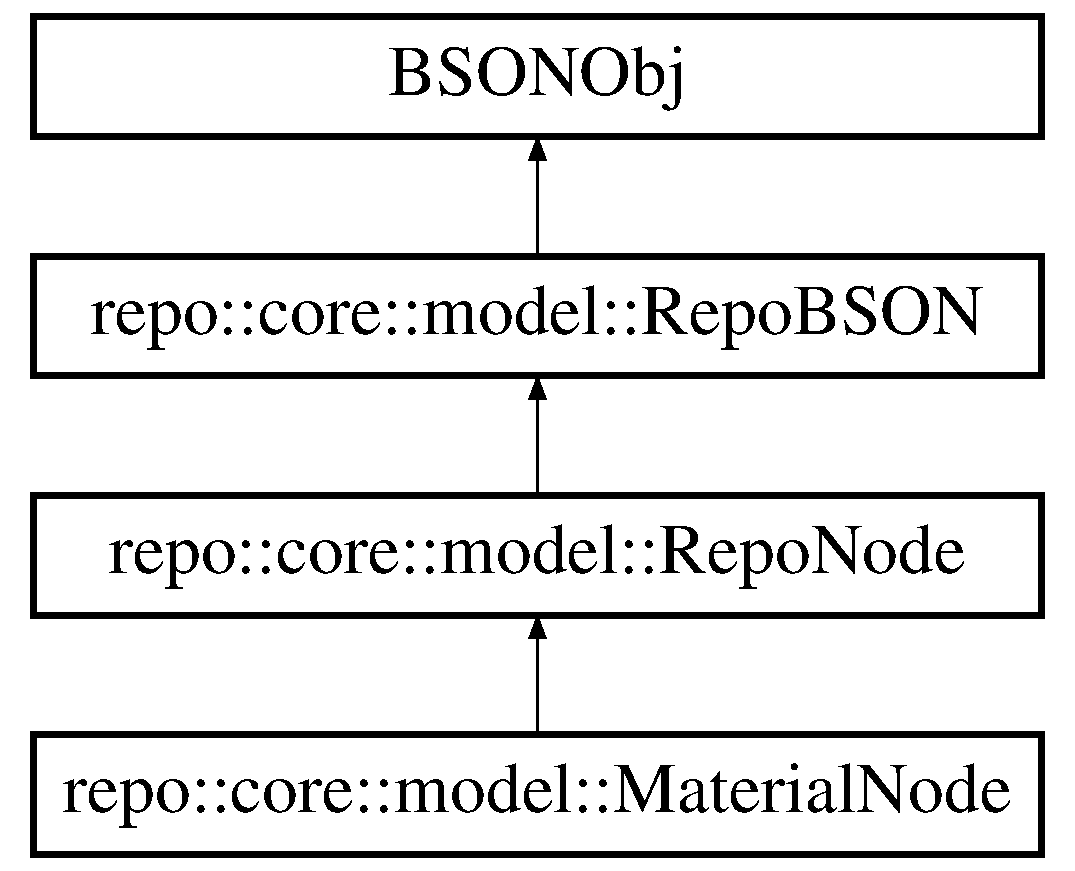
\includegraphics[height=4.000000cm]{classrepo_1_1core_1_1model_1_1_material_node}
\end{center}
\end{figure}
\subsection*{Public Member Functions}
\begin{DoxyCompactItemize}
\item 
\hyperlink{classrepo_1_1core_1_1model_1_1_material_node_a3a91d737bdf40a14c16e31de27efe2e8}{Material\+Node} ()
\item 
\hyperlink{classrepo_1_1core_1_1model_1_1_material_node_a24fbfaaba7b494de1c6ae9583a15f6a5}{Material\+Node} (\hyperlink{classrepo_1_1core_1_1model_1_1_repo_b_s_o_n}{Repo\+B\+S\+O\+N} bson)
\item 
\hyperlink{classrepo_1_1core_1_1model_1_1_material_node_a85d61ae04a894636d869560a02cefee5}{$\sim$\+Material\+Node} ()
\item 
virtual std\+::string \hyperlink{classrepo_1_1core_1_1model_1_1_material_node_af0debb10133049af18a7c1e45942b606}{get\+Type} () const 
\item 
virtual Node\+Type \hyperlink{classrepo_1_1core_1_1model_1_1_material_node_aa971c1eb43b76f95f28c063dac9919bc}{get\+Type\+As\+Enum} () const 
\item 
virtual bool \hyperlink{classrepo_1_1core_1_1model_1_1_material_node_a65fe37720ba763de81789f5c4f66039a}{s\+Equal} (const \hyperlink{classrepo_1_1core_1_1model_1_1_repo_node}{Repo\+Node} \&other) const 
\item 
\hyperlink{structrepo__material__t}{repo\+\_\+material\+\_\+t} \hyperlink{classrepo_1_1core_1_1model_1_1_material_node_a54c0685ffac3357c71f9a370aad37b43}{get\+Material\+Struct} () const 
\end{DoxyCompactItemize}
\subsection*{Protected Member Functions}
\begin{DoxyCompactItemize}
\item 
\hypertarget{classrepo_1_1core_1_1model_1_1_material_node_a8e50dc7e877713dcd0ef3adf6178ab72}{}std\+::vector$<$ float $>$ {\bfseries get\+Data\+As\+Buffer} () const \label{classrepo_1_1core_1_1model_1_1_material_node_a8e50dc7e877713dcd0ef3adf6178ab72}

\end{DoxyCompactItemize}
\subsection*{Additional Inherited Members}


\subsection{Constructor \& Destructor Documentation}
\hypertarget{classrepo_1_1core_1_1model_1_1_material_node_a3a91d737bdf40a14c16e31de27efe2e8}{}\index{repo\+::core\+::model\+::\+Material\+Node@{repo\+::core\+::model\+::\+Material\+Node}!Material\+Node@{Material\+Node}}
\index{Material\+Node@{Material\+Node}!repo\+::core\+::model\+::\+Material\+Node@{repo\+::core\+::model\+::\+Material\+Node}}
\subsubsection[{Material\+Node}]{\setlength{\rightskip}{0pt plus 5cm}Material\+Node\+::\+Material\+Node (
\begin{DoxyParamCaption}
{}
\end{DoxyParamCaption}
)}\label{classrepo_1_1core_1_1model_1_1_material_node_a3a91d737bdf40a14c16e31de27efe2e8}
Default constructor \hypertarget{classrepo_1_1core_1_1model_1_1_material_node_a24fbfaaba7b494de1c6ae9583a15f6a5}{}\index{repo\+::core\+::model\+::\+Material\+Node@{repo\+::core\+::model\+::\+Material\+Node}!Material\+Node@{Material\+Node}}
\index{Material\+Node@{Material\+Node}!repo\+::core\+::model\+::\+Material\+Node@{repo\+::core\+::model\+::\+Material\+Node}}
\subsubsection[{Material\+Node}]{\setlength{\rightskip}{0pt plus 5cm}Material\+Node\+::\+Material\+Node (
\begin{DoxyParamCaption}
\item[{{\bf Repo\+B\+S\+O\+N}}]{bson}
\end{DoxyParamCaption}
)}\label{classrepo_1_1core_1_1model_1_1_material_node_a24fbfaaba7b494de1c6ae9583a15f6a5}
Construct a \hyperlink{classrepo_1_1core_1_1model_1_1_material_node}{Material\+Node} from a \hyperlink{classrepo_1_1core_1_1model_1_1_repo_b_s_o_n}{Repo\+B\+S\+O\+N} object 
\begin{DoxyParams}{Parameters}
{\em \hyperlink{classrepo_1_1core_1_1model_1_1_repo_b_s_o_n}{Repo\+B\+S\+O\+N}} & object \\
\hline
\end{DoxyParams}
\hypertarget{classrepo_1_1core_1_1model_1_1_material_node_a85d61ae04a894636d869560a02cefee5}{}\index{repo\+::core\+::model\+::\+Material\+Node@{repo\+::core\+::model\+::\+Material\+Node}!````~Material\+Node@{$\sim$\+Material\+Node}}
\index{````~Material\+Node@{$\sim$\+Material\+Node}!repo\+::core\+::model\+::\+Material\+Node@{repo\+::core\+::model\+::\+Material\+Node}}
\subsubsection[{$\sim$\+Material\+Node}]{\setlength{\rightskip}{0pt plus 5cm}Material\+Node\+::$\sim$\+Material\+Node (
\begin{DoxyParamCaption}
{}
\end{DoxyParamCaption}
)}\label{classrepo_1_1core_1_1model_1_1_material_node_a85d61ae04a894636d869560a02cefee5}
Default deconstructor 

\subsection{Member Function Documentation}
\hypertarget{classrepo_1_1core_1_1model_1_1_material_node_a54c0685ffac3357c71f9a370aad37b43}{}\index{repo\+::core\+::model\+::\+Material\+Node@{repo\+::core\+::model\+::\+Material\+Node}!get\+Material\+Struct@{get\+Material\+Struct}}
\index{get\+Material\+Struct@{get\+Material\+Struct}!repo\+::core\+::model\+::\+Material\+Node@{repo\+::core\+::model\+::\+Material\+Node}}
\subsubsection[{get\+Material\+Struct}]{\setlength{\rightskip}{0pt plus 5cm}{\bf repo\+\_\+material\+\_\+t} Material\+Node\+::get\+Material\+Struct (
\begin{DoxyParamCaption}
{}
\end{DoxyParamCaption}
) const}\label{classrepo_1_1core_1_1model_1_1_material_node_a54c0685ffac3357c71f9a370aad37b43}
-\/-\/-\/------ Convenience functions -\/-\/-\/-\/-\/------ Get material information from the node as a struct \begin{DoxyReturn}{Returns}
returns a \hyperlink{structrepo__material__t}{repo\+\_\+material\+\_\+t} containing the information 
\end{DoxyReturn}
\hypertarget{classrepo_1_1core_1_1model_1_1_material_node_af0debb10133049af18a7c1e45942b606}{}\index{repo\+::core\+::model\+::\+Material\+Node@{repo\+::core\+::model\+::\+Material\+Node}!get\+Type@{get\+Type}}
\index{get\+Type@{get\+Type}!repo\+::core\+::model\+::\+Material\+Node@{repo\+::core\+::model\+::\+Material\+Node}}
\subsubsection[{get\+Type}]{\setlength{\rightskip}{0pt plus 5cm}virtual std\+::string repo\+::core\+::model\+::\+Material\+Node\+::get\+Type (
\begin{DoxyParamCaption}
{}
\end{DoxyParamCaption}
) const\hspace{0.3cm}{\ttfamily [inline]}, {\ttfamily [virtual]}}\label{classrepo_1_1core_1_1model_1_1_material_node_af0debb10133049af18a7c1e45942b606}
Get the type of node \begin{DoxyReturn}{Returns}
returns the type as a string 
\end{DoxyReturn}


Reimplemented from \hyperlink{classrepo_1_1core_1_1model_1_1_repo_node_a4380ba349235b5d9b13b41e41975805e}{repo\+::core\+::model\+::\+Repo\+Node}.

\hypertarget{classrepo_1_1core_1_1model_1_1_material_node_aa971c1eb43b76f95f28c063dac9919bc}{}\index{repo\+::core\+::model\+::\+Material\+Node@{repo\+::core\+::model\+::\+Material\+Node}!get\+Type\+As\+Enum@{get\+Type\+As\+Enum}}
\index{get\+Type\+As\+Enum@{get\+Type\+As\+Enum}!repo\+::core\+::model\+::\+Material\+Node@{repo\+::core\+::model\+::\+Material\+Node}}
\subsubsection[{get\+Type\+As\+Enum}]{\setlength{\rightskip}{0pt plus 5cm}virtual Node\+Type repo\+::core\+::model\+::\+Material\+Node\+::get\+Type\+As\+Enum (
\begin{DoxyParamCaption}
{}
\end{DoxyParamCaption}
) const\hspace{0.3cm}{\ttfamily [inline]}, {\ttfamily [virtual]}}\label{classrepo_1_1core_1_1model_1_1_material_node_aa971c1eb43b76f95f28c063dac9919bc}
Get the type of node as an enum \begin{DoxyReturn}{Returns}
returns type as enum. 
\end{DoxyReturn}


Reimplemented from \hyperlink{classrepo_1_1core_1_1model_1_1_repo_node_ad8d5295248dc9beb0b91efb2ce3b61f4}{repo\+::core\+::model\+::\+Repo\+Node}.

\hypertarget{classrepo_1_1core_1_1model_1_1_material_node_a65fe37720ba763de81789f5c4f66039a}{}\index{repo\+::core\+::model\+::\+Material\+Node@{repo\+::core\+::model\+::\+Material\+Node}!s\+Equal@{s\+Equal}}
\index{s\+Equal@{s\+Equal}!repo\+::core\+::model\+::\+Material\+Node@{repo\+::core\+::model\+::\+Material\+Node}}
\subsubsection[{s\+Equal}]{\setlength{\rightskip}{0pt plus 5cm}bool Material\+Node\+::s\+Equal (
\begin{DoxyParamCaption}
\item[{const {\bf Repo\+Node} \&}]{other}
\end{DoxyParamCaption}
) const\hspace{0.3cm}{\ttfamily [virtual]}}\label{classrepo_1_1core_1_1model_1_1_material_node_a65fe37720ba763de81789f5c4f66039a}
Check if the node is semantically equal to another Different node should have a different interpretation of what this means. 
\begin{DoxyParams}{Parameters}
{\em other} & node to compare with \\
\hline
{\em returns} & true if equal, false otherwise \\
\hline
\end{DoxyParams}


Reimplemented from \hyperlink{classrepo_1_1core_1_1model_1_1_repo_node_a7c98830a876ee6516587a8f07c7015a5}{repo\+::core\+::model\+::\+Repo\+Node}.



The documentation for this class was generated from the following files\+:\begin{DoxyCompactItemize}
\item 
C\+:/\+Users/\+Carmen/3\+D Repo/\+Repo/3drepobouncer/bouncer/src/repo/core/model/bson/repo\+\_\+node\+\_\+material.\+h\item 
C\+:/\+Users/\+Carmen/3\+D Repo/\+Repo/3drepobouncer/bouncer/src/repo/core/model/bson/repo\+\_\+node\+\_\+material.\+cpp\end{DoxyCompactItemize}

\hypertarget{classrepo_1_1manipulator_1_1modelutility_1_1_mesh_map_reorganiser}{}\section{repo\+:\+:manipulator\+:\+:modelutility\+:\+:Mesh\+Map\+Reorganiser Class Reference}
\label{classrepo_1_1manipulator_1_1modelutility_1_1_mesh_map_reorganiser}\index{repo\+::manipulator\+::modelutility\+::\+Mesh\+Map\+Reorganiser@{repo\+::manipulator\+::modelutility\+::\+Mesh\+Map\+Reorganiser}}
\subsection*{Public Member Functions}
\begin{DoxyCompactItemize}
\item 
\hyperlink{classrepo_1_1manipulator_1_1modelutility_1_1_mesh_map_reorganiser_a99f778aa78ba17e05caa3e22e4839f40}{Mesh\+Map\+Reorganiser} (const \hyperlink{classrepo_1_1core_1_1model_1_1_mesh_node}{repo\+::core\+::model\+::\+Mesh\+Node} $\ast$mesh, const size\+\_\+t \&vert\+Threshold)
\item 
std\+::vector$<$ std\+::vector$<$ float $>$ $>$ \hyperlink{classrepo_1_1manipulator_1_1modelutility_1_1_mesh_map_reorganiser_a30cbd2f8b0e24bc294be5e9def11b591}{get\+I\+D\+Map\+Arrays} () const 
\item 
std\+::vector$<$ std\+::vector$<$ \hyperlink{structrepo__mesh__mapping__t}{repo\+\_\+mesh\+\_\+mapping\+\_\+t} $>$ $>$ \hyperlink{classrepo_1_1manipulator_1_1modelutility_1_1_mesh_map_reorganiser_a7e05160f88ad0a1103cd7426f8aacd0d}{get\+Mappings\+Per\+Sub\+Mesh} () const 
\item 
\hyperlink{classrepo_1_1core_1_1model_1_1_mesh_node}{repo\+::core\+::model\+::\+Mesh\+Node} \hyperlink{classrepo_1_1manipulator_1_1modelutility_1_1_mesh_map_reorganiser_a29db789d0ad170041a5ecf4fd0dbd583}{get\+Remapped\+Mesh} () const 
\item 
std\+::vector$<$ uint16\+\_\+t $>$ \hyperlink{classrepo_1_1manipulator_1_1modelutility_1_1_mesh_map_reorganiser_a60fb9fad7e304bcfe6abfd5db1182b8b}{get\+Serialised\+Faces} () const 
\item 
std\+::unordered\+\_\+map$<$ repo\+U\+U\+I\+D, std\+::vector$<$ uint32\+\_\+t $>$, \hyperlink{struct_repo_u_u_i_d_hasher}{Repo\+U\+U\+I\+D\+Hasher} $>$ \hyperlink{classrepo_1_1manipulator_1_1modelutility_1_1_mesh_map_reorganiser_a8041d2c041c05563dfa0dd7528f09014}{get\+Split\+Mapping} () const 
\end{DoxyCompactItemize}


\subsection{Constructor \& Destructor Documentation}
\hypertarget{classrepo_1_1manipulator_1_1modelutility_1_1_mesh_map_reorganiser_a99f778aa78ba17e05caa3e22e4839f40}{}\index{repo\+::manipulator\+::modelutility\+::\+Mesh\+Map\+Reorganiser@{repo\+::manipulator\+::modelutility\+::\+Mesh\+Map\+Reorganiser}!Mesh\+Map\+Reorganiser@{Mesh\+Map\+Reorganiser}}
\index{Mesh\+Map\+Reorganiser@{Mesh\+Map\+Reorganiser}!repo\+::manipulator\+::modelutility\+::\+Mesh\+Map\+Reorganiser@{repo\+::manipulator\+::modelutility\+::\+Mesh\+Map\+Reorganiser}}
\subsubsection[{Mesh\+Map\+Reorganiser}]{\setlength{\rightskip}{0pt plus 5cm}Mesh\+Map\+Reorganiser\+::\+Mesh\+Map\+Reorganiser (
\begin{DoxyParamCaption}
\item[{const {\bf repo\+::core\+::model\+::\+Mesh\+Node} $\ast$}]{mesh, }
\item[{const size\+\_\+t \&}]{vert\+Threshold}
\end{DoxyParamCaption}
)}\label{classrepo_1_1manipulator_1_1modelutility_1_1_mesh_map_reorganiser_a99f778aa78ba17e05caa3e22e4839f40}
Construct a mesh reorganiser if the reorganiser failed to generate a remapped mesh, it will return an empty mesh\+Node. 
\begin{DoxyParams}{Parameters}
{\em mesh} & the mesh to reorganise \\
\hline
{\em vert\+Threshold} & maximum vertices \\
\hline
\end{DoxyParams}


\subsection{Member Function Documentation}
\hypertarget{classrepo_1_1manipulator_1_1modelutility_1_1_mesh_map_reorganiser_a30cbd2f8b0e24bc294be5e9def11b591}{}\index{repo\+::manipulator\+::modelutility\+::\+Mesh\+Map\+Reorganiser@{repo\+::manipulator\+::modelutility\+::\+Mesh\+Map\+Reorganiser}!get\+I\+D\+Map\+Arrays@{get\+I\+D\+Map\+Arrays}}
\index{get\+I\+D\+Map\+Arrays@{get\+I\+D\+Map\+Arrays}!repo\+::manipulator\+::modelutility\+::\+Mesh\+Map\+Reorganiser@{repo\+::manipulator\+::modelutility\+::\+Mesh\+Map\+Reorganiser}}
\subsubsection[{get\+I\+D\+Map\+Arrays}]{\setlength{\rightskip}{0pt plus 5cm}std\+::vector$<$ std\+::vector$<$ float $>$ $>$ Mesh\+Map\+Reorganiser\+::get\+I\+D\+Map\+Arrays (
\begin{DoxyParamCaption}
{}
\end{DoxyParamCaption}
) const}\label{classrepo_1_1manipulator_1_1modelutility_1_1_mesh_map_reorganiser_a30cbd2f8b0e24bc294be5e9def11b591}
Return id\+Map arrays of the modified mesh (for material mapping) \begin{DoxyReturn}{Returns}
returns a id\+Map arrays 
\end{DoxyReturn}
\hypertarget{classrepo_1_1manipulator_1_1modelutility_1_1_mesh_map_reorganiser_a7e05160f88ad0a1103cd7426f8aacd0d}{}\index{repo\+::manipulator\+::modelutility\+::\+Mesh\+Map\+Reorganiser@{repo\+::manipulator\+::modelutility\+::\+Mesh\+Map\+Reorganiser}!get\+Mappings\+Per\+Sub\+Mesh@{get\+Mappings\+Per\+Sub\+Mesh}}
\index{get\+Mappings\+Per\+Sub\+Mesh@{get\+Mappings\+Per\+Sub\+Mesh}!repo\+::manipulator\+::modelutility\+::\+Mesh\+Map\+Reorganiser@{repo\+::manipulator\+::modelutility\+::\+Mesh\+Map\+Reorganiser}}
\subsubsection[{get\+Mappings\+Per\+Sub\+Mesh}]{\setlength{\rightskip}{0pt plus 5cm}std\+::vector$<$ std\+::vector$<$ {\bf repo\+\_\+mesh\+\_\+mapping\+\_\+t} $>$ $>$ Mesh\+Map\+Reorganiser\+::get\+Mappings\+Per\+Sub\+Mesh (
\begin{DoxyParamCaption}
{}
\end{DoxyParamCaption}
) const}\label{classrepo_1_1manipulator_1_1modelutility_1_1_mesh_map_reorganiser_a7e05160f88ad0a1103cd7426f8aacd0d}
Get all mesh mapping, grouped by the sub meshes they belong to \begin{DoxyReturn}{Returns}
a vector (new submeshes) of vector of mesh mappings(original submeshes) 
\end{DoxyReturn}
\hypertarget{classrepo_1_1manipulator_1_1modelutility_1_1_mesh_map_reorganiser_a29db789d0ad170041a5ecf4fd0dbd583}{}\index{repo\+::manipulator\+::modelutility\+::\+Mesh\+Map\+Reorganiser@{repo\+::manipulator\+::modelutility\+::\+Mesh\+Map\+Reorganiser}!get\+Remapped\+Mesh@{get\+Remapped\+Mesh}}
\index{get\+Remapped\+Mesh@{get\+Remapped\+Mesh}!repo\+::manipulator\+::modelutility\+::\+Mesh\+Map\+Reorganiser@{repo\+::manipulator\+::modelutility\+::\+Mesh\+Map\+Reorganiser}}
\subsubsection[{get\+Remapped\+Mesh}]{\setlength{\rightskip}{0pt plus 5cm}{\bf repo\+::core\+::model\+::\+Mesh\+Node} Mesh\+Map\+Reorganiser\+::get\+Remapped\+Mesh (
\begin{DoxyParamCaption}
{}
\end{DoxyParamCaption}
) const}\label{classrepo_1_1manipulator_1_1modelutility_1_1_mesh_map_reorganiser_a29db789d0ad170041a5ecf4fd0dbd583}
Get the mesh, with mesh mappings and buffers modified \begin{DoxyReturn}{Returns}
returns the modified mesh 
\end{DoxyReturn}
\hypertarget{classrepo_1_1manipulator_1_1modelutility_1_1_mesh_map_reorganiser_a60fb9fad7e304bcfe6abfd5db1182b8b}{}\index{repo\+::manipulator\+::modelutility\+::\+Mesh\+Map\+Reorganiser@{repo\+::manipulator\+::modelutility\+::\+Mesh\+Map\+Reorganiser}!get\+Serialised\+Faces@{get\+Serialised\+Faces}}
\index{get\+Serialised\+Faces@{get\+Serialised\+Faces}!repo\+::manipulator\+::modelutility\+::\+Mesh\+Map\+Reorganiser@{repo\+::manipulator\+::modelutility\+::\+Mesh\+Map\+Reorganiser}}
\subsubsection[{get\+Serialised\+Faces}]{\setlength{\rightskip}{0pt plus 5cm}std\+::vector$<$ uint16\+\_\+t $>$ Mesh\+Map\+Reorganiser\+::get\+Serialised\+Faces (
\begin{DoxyParamCaption}
{}
\end{DoxyParamCaption}
) const}\label{classrepo_1_1manipulator_1_1modelutility_1_1_mesh_map_reorganiser_a60fb9fad7e304bcfe6abfd5db1182b8b}
Return serialised faces of the modified mesh \begin{DoxyReturn}{Returns}
returns a serialised buffer of faces 
\end{DoxyReturn}
\hypertarget{classrepo_1_1manipulator_1_1modelutility_1_1_mesh_map_reorganiser_a8041d2c041c05563dfa0dd7528f09014}{}\index{repo\+::manipulator\+::modelutility\+::\+Mesh\+Map\+Reorganiser@{repo\+::manipulator\+::modelutility\+::\+Mesh\+Map\+Reorganiser}!get\+Split\+Mapping@{get\+Split\+Mapping}}
\index{get\+Split\+Mapping@{get\+Split\+Mapping}!repo\+::manipulator\+::modelutility\+::\+Mesh\+Map\+Reorganiser@{repo\+::manipulator\+::modelutility\+::\+Mesh\+Map\+Reorganiser}}
\subsubsection[{get\+Split\+Mapping}]{\setlength{\rightskip}{0pt plus 5cm}std\+::unordered\+\_\+map$<$ repo\+U\+U\+I\+D, std\+::vector$<$ uint32\+\_\+t $>$, {\bf Repo\+U\+U\+I\+D\+Hasher} $>$ Mesh\+Map\+Reorganiser\+::get\+Split\+Mapping (
\begin{DoxyParamCaption}
{}
\end{DoxyParamCaption}
) const}\label{classrepo_1_1manipulator_1_1modelutility_1_1_mesh_map_reorganiser_a8041d2c041c05563dfa0dd7528f09014}
Get the mapping between submeshes U\+U\+I\+D to new super mesh index \begin{DoxyReturn}{Returns}
sub mesh to super mesh(es) mapping 
\end{DoxyReturn}


The documentation for this class was generated from the following files\+:\begin{DoxyCompactItemize}
\item 
C\+:/\+Users/\+Carmen/3\+D Repo/\+Repo/3drepobouncer/bouncer/src/repo/manipulator/modelutility/repo\+\_\+mesh\+\_\+map\+\_\+reorganiser.\+h\item 
C\+:/\+Users/\+Carmen/3\+D Repo/\+Repo/3drepobouncer/bouncer/src/repo/manipulator/modelutility/repo\+\_\+mesh\+\_\+map\+\_\+reorganiser.\+cpp\end{DoxyCompactItemize}

\hypertarget{classrepo_1_1core_1_1model_1_1_mesh_node}{}\section{repo\+:\+:core\+:\+:model\+:\+:Mesh\+Node Class Reference}
\label{classrepo_1_1core_1_1model_1_1_mesh_node}\index{repo\+::core\+::model\+::\+Mesh\+Node@{repo\+::core\+::model\+::\+Mesh\+Node}}
Inheritance diagram for repo\+:\+:core\+:\+:model\+:\+:Mesh\+Node\+:\begin{figure}[H]
\begin{center}
\leavevmode
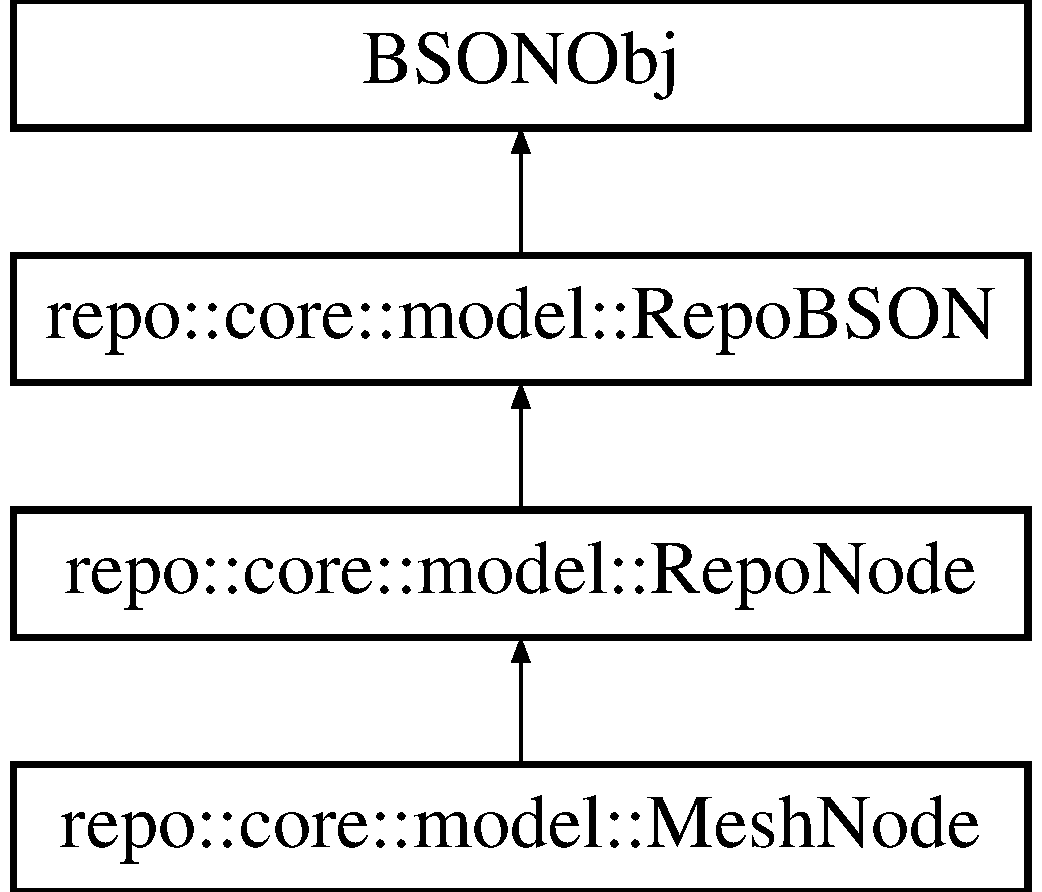
\includegraphics[height=4.000000cm]{classrepo_1_1core_1_1model_1_1_mesh_node}
\end{center}
\end{figure}
\subsection*{Public Member Functions}
\begin{DoxyCompactItemize}
\item 
\hyperlink{classrepo_1_1core_1_1model_1_1_mesh_node_ab525cdafcb942a4c79eb517b7ef0f5c7}{Mesh\+Node} ()
\item 
\hyperlink{classrepo_1_1core_1_1model_1_1_mesh_node_a2612d3a4561a24d3b31a9a7de87daf3c}{Mesh\+Node} (\hyperlink{classrepo_1_1core_1_1model_1_1_repo_b_s_o_n}{Repo\+B\+S\+O\+N} bson, const std\+::unordered\+\_\+map$<$ std\+::string, std\+::pair$<$ std\+::string, std\+::vector$<$ uint8\+\_\+t $>$$>$$>$ \&bin\+Mapping=std\+::unordered\+\_\+map$<$ std\+::string, std\+::pair$<$ std\+::string, std\+::vector$<$ uint8\+\_\+t $>$$>$$>$())
\item 
\hyperlink{classrepo_1_1core_1_1model_1_1_mesh_node_abf8b858b11632dc9827b3ffa1cdc8c9b}{$\sim$\+Mesh\+Node} ()
\item 
uint32\+\_\+t \hyperlink{classrepo_1_1core_1_1model_1_1_mesh_node_af55de353138ad754ad2ce9b237010354}{get\+M\+Format} () const 
\item 
virtual std\+::string \hyperlink{classrepo_1_1core_1_1model_1_1_mesh_node_afb8fedac41e86bce0f74509efa6d9614}{get\+Type} () const 
\item 
virtual Node\+Type \hyperlink{classrepo_1_1core_1_1model_1_1_mesh_node_aba656559a131b00514ca844a7e8a595c}{get\+Type\+As\+Enum} () const 
\item 
virtual bool \hyperlink{classrepo_1_1core_1_1model_1_1_mesh_node_a636fc543dbbeca60698e8719c11f945d}{position\+Dependant} ()
\item 
virtual bool \hyperlink{classrepo_1_1core_1_1model_1_1_mesh_node_a58dbc8bb0cdcbbae2e0c6e7558eaef70}{s\+Equal} (const \hyperlink{classrepo_1_1core_1_1model_1_1_repo_node}{Repo\+Node} \&other) const 
\item 
virtual \hyperlink{classrepo_1_1core_1_1model_1_1_repo_node}{Repo\+Node} \hyperlink{classrepo_1_1core_1_1model_1_1_mesh_node_a8f65c14c0c964ee17197135e95e30e3c}{clone\+And\+Apply\+Transformation} (const std\+::vector$<$ float $>$ \&matrix) const 
\item 
\hyperlink{classrepo_1_1core_1_1model_1_1_mesh_node}{Mesh\+Node} \hyperlink{classrepo_1_1core_1_1model_1_1_mesh_node_a7a0ed7c54172f0bab82732c884b8199d}{clone\+And\+Update\+Mesh\+Mapping} (const std\+::vector$<$ \hyperlink{structrepo__mesh__mapping__t}{repo\+\_\+mesh\+\_\+mapping\+\_\+t} $>$ \&vec, const bool \&overwrite=false)
\item 
std\+::vector$<$ \hyperlink{structrepo__vector__t}{repo\+\_\+vector\+\_\+t} $>$ \hyperlink{classrepo_1_1core_1_1model_1_1_mesh_node_a9a8d98653f384b8a0a642aec5f14665b}{get\+Bounding\+Box} () const 
\item 
std\+::vector$<$ \hyperlink{structrepo__color4d__t}{repo\+\_\+color4d\+\_\+t} $>$ \hyperlink{classrepo_1_1core_1_1model_1_1_mesh_node_a0fbecdd9cde9c11e4faae613657040b1}{get\+Colors} () const 
\item 
std\+::vector$<$ repo\+\_\+face\+\_\+t $>$ \hyperlink{classrepo_1_1core_1_1model_1_1_mesh_node_ab542b62a7ef4ea7f45a49769e679e999}{get\+Faces} () const 
\item 
\hypertarget{classrepo_1_1core_1_1model_1_1_mesh_node_acfb7939da55a97f8f070503fd03bbef5}{}std\+::vector$<$ \hyperlink{structrepo__mesh__mapping__t}{repo\+\_\+mesh\+\_\+mapping\+\_\+t} $>$ {\bfseries get\+Mesh\+Mapping} () const \label{classrepo_1_1core_1_1model_1_1_mesh_node_acfb7939da55a97f8f070503fd03bbef5}

\item 
std\+::vector$<$ \hyperlink{structrepo__vector__t}{repo\+\_\+vector\+\_\+t} $>$ \hyperlink{classrepo_1_1core_1_1model_1_1_mesh_node_a4cc4020f392b6ff3f033a65fc6ae95d9}{get\+Normals} () const 
\item 
std\+::vector$<$ \hyperlink{structrepo__vector2d__t}{repo\+\_\+vector2d\+\_\+t} $>$ \hyperlink{classrepo_1_1core_1_1model_1_1_mesh_node_a339a7467aba5856f31114dcae49f688b}{get\+U\+V\+Channels} () const 
\item 
std\+::vector$<$ std\+::vector$<$ \hyperlink{structrepo__vector2d__t}{repo\+\_\+vector2d\+\_\+t} $>$ $>$ \hyperlink{classrepo_1_1core_1_1model_1_1_mesh_node_ac3b3b4fc307f3eb64fde27ce39f8daed}{get\+U\+V\+Channels\+Separated} () const 
\item 
std\+::vector$<$ \hyperlink{structrepo__vector__t}{repo\+\_\+vector\+\_\+t} $>$ \hyperlink{classrepo_1_1core_1_1model_1_1_mesh_node_a2b03157eecf7bdf41534db3068178d05}{get\+Vertices} () const 
\end{DoxyCompactItemize}
\subsection*{Static Public Member Functions}
\begin{DoxyCompactItemize}
\item 
\hypertarget{classrepo_1_1core_1_1model_1_1_mesh_node_a77196efc86472f9ec298935f89d78ac8}{}static std\+::vector$<$ \hyperlink{structrepo__vector__t}{repo\+\_\+vector\+\_\+t} $>$ {\bfseries get\+Bounding\+Box} (\hyperlink{classrepo_1_1core_1_1model_1_1_repo_b_s_o_n}{Repo\+B\+S\+O\+N} \&bb\+Arr)\label{classrepo_1_1core_1_1model_1_1_mesh_node_a77196efc86472f9ec298935f89d78ac8}

\end{DoxyCompactItemize}
\subsection*{Additional Inherited Members}


\subsection{Constructor \& Destructor Documentation}
\hypertarget{classrepo_1_1core_1_1model_1_1_mesh_node_ab525cdafcb942a4c79eb517b7ef0f5c7}{}\index{repo\+::core\+::model\+::\+Mesh\+Node@{repo\+::core\+::model\+::\+Mesh\+Node}!Mesh\+Node@{Mesh\+Node}}
\index{Mesh\+Node@{Mesh\+Node}!repo\+::core\+::model\+::\+Mesh\+Node@{repo\+::core\+::model\+::\+Mesh\+Node}}
\subsubsection[{Mesh\+Node}]{\setlength{\rightskip}{0pt plus 5cm}Mesh\+Node\+::\+Mesh\+Node (
\begin{DoxyParamCaption}
{}
\end{DoxyParamCaption}
)}\label{classrepo_1_1core_1_1model_1_1_mesh_node_ab525cdafcb942a4c79eb517b7ef0f5c7}
Default constructor \hypertarget{classrepo_1_1core_1_1model_1_1_mesh_node_a2612d3a4561a24d3b31a9a7de87daf3c}{}\index{repo\+::core\+::model\+::\+Mesh\+Node@{repo\+::core\+::model\+::\+Mesh\+Node}!Mesh\+Node@{Mesh\+Node}}
\index{Mesh\+Node@{Mesh\+Node}!repo\+::core\+::model\+::\+Mesh\+Node@{repo\+::core\+::model\+::\+Mesh\+Node}}
\subsubsection[{Mesh\+Node}]{\setlength{\rightskip}{0pt plus 5cm}Mesh\+Node\+::\+Mesh\+Node (
\begin{DoxyParamCaption}
\item[{{\bf Repo\+B\+S\+O\+N}}]{bson, }
\item[{const std\+::unordered\+\_\+map$<$ std\+::string, std\+::pair$<$ std\+::string, std\+::vector$<$ uint8\+\_\+t $>$$>$$>$ \&}]{bin\+Mapping = {\ttfamily std\+:\+:unordered\+\_\+map$<$std\+:\+:string,~std\+:\+:pair$<$std\+:\+:string,~std\+:\+:vector$<$uint8\+\_\+t$>$$>$$>$()}}
\end{DoxyParamCaption}
)}\label{classrepo_1_1core_1_1model_1_1_mesh_node_a2612d3a4561a24d3b31a9a7de87daf3c}
Construct a \hyperlink{classrepo_1_1core_1_1model_1_1_mesh_node}{Mesh\+Node} from a \hyperlink{classrepo_1_1core_1_1model_1_1_repo_b_s_o_n}{Repo\+B\+S\+O\+N} object 
\begin{DoxyParams}{Parameters}
{\em \hyperlink{classrepo_1_1core_1_1model_1_1_repo_b_s_o_n}{Repo\+B\+S\+O\+N}} & object \\
\hline
{\em bin\+Mapping} & binary mapping of fields that are too big to fit within the bson \\
\hline
\end{DoxyParams}
\hypertarget{classrepo_1_1core_1_1model_1_1_mesh_node_abf8b858b11632dc9827b3ffa1cdc8c9b}{}\index{repo\+::core\+::model\+::\+Mesh\+Node@{repo\+::core\+::model\+::\+Mesh\+Node}!````~Mesh\+Node@{$\sim$\+Mesh\+Node}}
\index{````~Mesh\+Node@{$\sim$\+Mesh\+Node}!repo\+::core\+::model\+::\+Mesh\+Node@{repo\+::core\+::model\+::\+Mesh\+Node}}
\subsubsection[{$\sim$\+Mesh\+Node}]{\setlength{\rightskip}{0pt plus 5cm}Mesh\+Node\+::$\sim$\+Mesh\+Node (
\begin{DoxyParamCaption}
{}
\end{DoxyParamCaption}
)}\label{classrepo_1_1core_1_1model_1_1_mesh_node_abf8b858b11632dc9827b3ffa1cdc8c9b}
Default deconstructor 

\subsection{Member Function Documentation}
\hypertarget{classrepo_1_1core_1_1model_1_1_mesh_node_a8f65c14c0c964ee17197135e95e30e3c}{}\index{repo\+::core\+::model\+::\+Mesh\+Node@{repo\+::core\+::model\+::\+Mesh\+Node}!clone\+And\+Apply\+Transformation@{clone\+And\+Apply\+Transformation}}
\index{clone\+And\+Apply\+Transformation@{clone\+And\+Apply\+Transformation}!repo\+::core\+::model\+::\+Mesh\+Node@{repo\+::core\+::model\+::\+Mesh\+Node}}
\subsubsection[{clone\+And\+Apply\+Transformation}]{\setlength{\rightskip}{0pt plus 5cm}{\bf Repo\+Node} Mesh\+Node\+::clone\+And\+Apply\+Transformation (
\begin{DoxyParamCaption}
\item[{const std\+::vector$<$ float $>$ \&}]{matrix}
\end{DoxyParamCaption}
) const\hspace{0.3cm}{\ttfamily [virtual]}}\label{classrepo_1_1core_1_1model_1_1_mesh_node_a8f65c14c0c964ee17197135e95e30e3c}
Create a new object with transformation applied to the node default behaviour is do nothing. Children object needs to override this function to perform their own specific behaviour. 
\begin{DoxyParams}{Parameters}
{\em matrix} & transformation matrix to apply. \\
\hline
\end{DoxyParams}
\begin{DoxyReturn}{Returns}
returns a new object with transformation applied. 
\end{DoxyReturn}


Reimplemented from \hyperlink{classrepo_1_1core_1_1model_1_1_repo_node_ac31acdb9774bce9296cb5005286db83d}{repo\+::core\+::model\+::\+Repo\+Node}.

\hypertarget{classrepo_1_1core_1_1model_1_1_mesh_node_a7a0ed7c54172f0bab82732c884b8199d}{}\index{repo\+::core\+::model\+::\+Mesh\+Node@{repo\+::core\+::model\+::\+Mesh\+Node}!clone\+And\+Update\+Mesh\+Mapping@{clone\+And\+Update\+Mesh\+Mapping}}
\index{clone\+And\+Update\+Mesh\+Mapping@{clone\+And\+Update\+Mesh\+Mapping}!repo\+::core\+::model\+::\+Mesh\+Node@{repo\+::core\+::model\+::\+Mesh\+Node}}
\subsubsection[{clone\+And\+Update\+Mesh\+Mapping}]{\setlength{\rightskip}{0pt plus 5cm}{\bf Mesh\+Node} Mesh\+Node\+::clone\+And\+Update\+Mesh\+Mapping (
\begin{DoxyParamCaption}
\item[{const std\+::vector$<$ {\bf repo\+\_\+mesh\+\_\+mapping\+\_\+t} $>$ \&}]{vec, }
\item[{const bool \&}]{overwrite = {\ttfamily false}}
\end{DoxyParamCaption}
)}\label{classrepo_1_1core_1_1model_1_1_mesh_node_a7a0ed7c54172f0bab82732c884b8199d}
Create a new copy of the node and update its mesh mapping \begin{DoxyReturn}{Returns}
returns a new mesh\+Node with the new mappings 
\end{DoxyReturn}
\hypertarget{classrepo_1_1core_1_1model_1_1_mesh_node_a9a8d98653f384b8a0a642aec5f14665b}{}\index{repo\+::core\+::model\+::\+Mesh\+Node@{repo\+::core\+::model\+::\+Mesh\+Node}!get\+Bounding\+Box@{get\+Bounding\+Box}}
\index{get\+Bounding\+Box@{get\+Bounding\+Box}!repo\+::core\+::model\+::\+Mesh\+Node@{repo\+::core\+::model\+::\+Mesh\+Node}}
\subsubsection[{get\+Bounding\+Box}]{\setlength{\rightskip}{0pt plus 5cm}std\+::vector$<$ {\bf repo\+\_\+vector\+\_\+t} $>$ Mesh\+Node\+::get\+Bounding\+Box (
\begin{DoxyParamCaption}
{}
\end{DoxyParamCaption}
) const}\label{classrepo_1_1core_1_1model_1_1_mesh_node_a9a8d98653f384b8a0a642aec5f14665b}
-\/-\/-\/------ Convenience functions -\/-\/-\/-\/-\/------ Retrieve the bounding box of this mesh \begin{DoxyReturn}{Returns}
returns a vector of size 2, containing the bounding box. 
\end{DoxyReturn}
\hypertarget{classrepo_1_1core_1_1model_1_1_mesh_node_a0fbecdd9cde9c11e4faae613657040b1}{}\index{repo\+::core\+::model\+::\+Mesh\+Node@{repo\+::core\+::model\+::\+Mesh\+Node}!get\+Colors@{get\+Colors}}
\index{get\+Colors@{get\+Colors}!repo\+::core\+::model\+::\+Mesh\+Node@{repo\+::core\+::model\+::\+Mesh\+Node}}
\subsubsection[{get\+Colors}]{\setlength{\rightskip}{0pt plus 5cm}std\+::vector$<$ {\bf repo\+\_\+color4d\+\_\+t} $>$ Mesh\+Node\+::get\+Colors (
\begin{DoxyParamCaption}
{}
\end{DoxyParamCaption}
) const}\label{classrepo_1_1core_1_1model_1_1_mesh_node_a0fbecdd9cde9c11e4faae613657040b1}
Retrieve a vector of Colors from the bson object \hypertarget{classrepo_1_1core_1_1model_1_1_mesh_node_ab542b62a7ef4ea7f45a49769e679e999}{}\index{repo\+::core\+::model\+::\+Mesh\+Node@{repo\+::core\+::model\+::\+Mesh\+Node}!get\+Faces@{get\+Faces}}
\index{get\+Faces@{get\+Faces}!repo\+::core\+::model\+::\+Mesh\+Node@{repo\+::core\+::model\+::\+Mesh\+Node}}
\subsubsection[{get\+Faces}]{\setlength{\rightskip}{0pt plus 5cm}std\+::vector$<$ repo\+\_\+face\+\_\+t $>$ Mesh\+Node\+::get\+Faces (
\begin{DoxyParamCaption}
{}
\end{DoxyParamCaption}
) const}\label{classrepo_1_1core_1_1model_1_1_mesh_node_ab542b62a7ef4ea7f45a49769e679e999}
Retrieve a vector of faces from the bson object \hypertarget{classrepo_1_1core_1_1model_1_1_mesh_node_af55de353138ad754ad2ce9b237010354}{}\index{repo\+::core\+::model\+::\+Mesh\+Node@{repo\+::core\+::model\+::\+Mesh\+Node}!get\+M\+Format@{get\+M\+Format}}
\index{get\+M\+Format@{get\+M\+Format}!repo\+::core\+::model\+::\+Mesh\+Node@{repo\+::core\+::model\+::\+Mesh\+Node}}
\subsubsection[{get\+M\+Format}]{\setlength{\rightskip}{0pt plus 5cm}uint32\+\_\+t Mesh\+Node\+::get\+M\+Format (
\begin{DoxyParamCaption}
{}
\end{DoxyParamCaption}
) const}\label{classrepo_1_1core_1_1model_1_1_mesh_node_af55de353138ad754ad2ce9b237010354}
Returns a number, indicating it\textquotesingle{}s mesh format maximum of 32 bit, each bit represent the presents of the following vertices faces normals colors \#uvs where vertices is the L\+S\+B \begin{DoxyReturn}{Returns}
returns the m\+Format flag 
\end{DoxyReturn}
\hypertarget{classrepo_1_1core_1_1model_1_1_mesh_node_a4cc4020f392b6ff3f033a65fc6ae95d9}{}\index{repo\+::core\+::model\+::\+Mesh\+Node@{repo\+::core\+::model\+::\+Mesh\+Node}!get\+Normals@{get\+Normals}}
\index{get\+Normals@{get\+Normals}!repo\+::core\+::model\+::\+Mesh\+Node@{repo\+::core\+::model\+::\+Mesh\+Node}}
\subsubsection[{get\+Normals}]{\setlength{\rightskip}{0pt plus 5cm}std\+::vector$<$ {\bf repo\+\_\+vector\+\_\+t} $>$ Mesh\+Node\+::get\+Normals (
\begin{DoxyParamCaption}
{}
\end{DoxyParamCaption}
) const}\label{classrepo_1_1core_1_1model_1_1_mesh_node_a4cc4020f392b6ff3f033a65fc6ae95d9}
Retrieve a vector of vertices from the bson object \hypertarget{classrepo_1_1core_1_1model_1_1_mesh_node_afb8fedac41e86bce0f74509efa6d9614}{}\index{repo\+::core\+::model\+::\+Mesh\+Node@{repo\+::core\+::model\+::\+Mesh\+Node}!get\+Type@{get\+Type}}
\index{get\+Type@{get\+Type}!repo\+::core\+::model\+::\+Mesh\+Node@{repo\+::core\+::model\+::\+Mesh\+Node}}
\subsubsection[{get\+Type}]{\setlength{\rightskip}{0pt plus 5cm}virtual std\+::string repo\+::core\+::model\+::\+Mesh\+Node\+::get\+Type (
\begin{DoxyParamCaption}
{}
\end{DoxyParamCaption}
) const\hspace{0.3cm}{\ttfamily [inline]}, {\ttfamily [virtual]}}\label{classrepo_1_1core_1_1model_1_1_mesh_node_afb8fedac41e86bce0f74509efa6d9614}
Get the type of node \begin{DoxyReturn}{Returns}
returns the type as a string 
\end{DoxyReturn}


Reimplemented from \hyperlink{classrepo_1_1core_1_1model_1_1_repo_node_a4380ba349235b5d9b13b41e41975805e}{repo\+::core\+::model\+::\+Repo\+Node}.

\hypertarget{classrepo_1_1core_1_1model_1_1_mesh_node_aba656559a131b00514ca844a7e8a595c}{}\index{repo\+::core\+::model\+::\+Mesh\+Node@{repo\+::core\+::model\+::\+Mesh\+Node}!get\+Type\+As\+Enum@{get\+Type\+As\+Enum}}
\index{get\+Type\+As\+Enum@{get\+Type\+As\+Enum}!repo\+::core\+::model\+::\+Mesh\+Node@{repo\+::core\+::model\+::\+Mesh\+Node}}
\subsubsection[{get\+Type\+As\+Enum}]{\setlength{\rightskip}{0pt plus 5cm}virtual Node\+Type repo\+::core\+::model\+::\+Mesh\+Node\+::get\+Type\+As\+Enum (
\begin{DoxyParamCaption}
{}
\end{DoxyParamCaption}
) const\hspace{0.3cm}{\ttfamily [inline]}, {\ttfamily [virtual]}}\label{classrepo_1_1core_1_1model_1_1_mesh_node_aba656559a131b00514ca844a7e8a595c}
Get the type of node as an enum \begin{DoxyReturn}{Returns}
returns type as enum. 
\end{DoxyReturn}


Reimplemented from \hyperlink{classrepo_1_1core_1_1model_1_1_repo_node_ad8d5295248dc9beb0b91efb2ce3b61f4}{repo\+::core\+::model\+::\+Repo\+Node}.

\hypertarget{classrepo_1_1core_1_1model_1_1_mesh_node_a339a7467aba5856f31114dcae49f688b}{}\index{repo\+::core\+::model\+::\+Mesh\+Node@{repo\+::core\+::model\+::\+Mesh\+Node}!get\+U\+V\+Channels@{get\+U\+V\+Channels}}
\index{get\+U\+V\+Channels@{get\+U\+V\+Channels}!repo\+::core\+::model\+::\+Mesh\+Node@{repo\+::core\+::model\+::\+Mesh\+Node}}
\subsubsection[{get\+U\+V\+Channels}]{\setlength{\rightskip}{0pt plus 5cm}std\+::vector$<$ {\bf repo\+\_\+vector2d\+\_\+t} $>$ Mesh\+Node\+::get\+U\+V\+Channels (
\begin{DoxyParamCaption}
{}
\end{DoxyParamCaption}
) const}\label{classrepo_1_1core_1_1model_1_1_mesh_node_a339a7467aba5856f31114dcae49f688b}
Retrieve a vector of U\+V Channels from the bson object \hypertarget{classrepo_1_1core_1_1model_1_1_mesh_node_ac3b3b4fc307f3eb64fde27ce39f8daed}{}\index{repo\+::core\+::model\+::\+Mesh\+Node@{repo\+::core\+::model\+::\+Mesh\+Node}!get\+U\+V\+Channels\+Separated@{get\+U\+V\+Channels\+Separated}}
\index{get\+U\+V\+Channels\+Separated@{get\+U\+V\+Channels\+Separated}!repo\+::core\+::model\+::\+Mesh\+Node@{repo\+::core\+::model\+::\+Mesh\+Node}}
\subsubsection[{get\+U\+V\+Channels\+Separated}]{\setlength{\rightskip}{0pt plus 5cm}std\+::vector$<$ std\+::vector$<$ {\bf repo\+\_\+vector2d\+\_\+t} $>$ $>$ Mesh\+Node\+::get\+U\+V\+Channels\+Separated (
\begin{DoxyParamCaption}
{}
\end{DoxyParamCaption}
) const}\label{classrepo_1_1core_1_1model_1_1_mesh_node_ac3b3b4fc307f3eb64fde27ce39f8daed}
Retrieve a vector of U\+V Channels, separated by channels \hypertarget{classrepo_1_1core_1_1model_1_1_mesh_node_a2b03157eecf7bdf41534db3068178d05}{}\index{repo\+::core\+::model\+::\+Mesh\+Node@{repo\+::core\+::model\+::\+Mesh\+Node}!get\+Vertices@{get\+Vertices}}
\index{get\+Vertices@{get\+Vertices}!repo\+::core\+::model\+::\+Mesh\+Node@{repo\+::core\+::model\+::\+Mesh\+Node}}
\subsubsection[{get\+Vertices}]{\setlength{\rightskip}{0pt plus 5cm}std\+::vector$<$ {\bf repo\+\_\+vector\+\_\+t} $>$ Mesh\+Node\+::get\+Vertices (
\begin{DoxyParamCaption}
{}
\end{DoxyParamCaption}
) const}\label{classrepo_1_1core_1_1model_1_1_mesh_node_a2b03157eecf7bdf41534db3068178d05}
Retrieve a vector of vertices from the bson object \hypertarget{classrepo_1_1core_1_1model_1_1_mesh_node_a636fc543dbbeca60698e8719c11f945d}{}\index{repo\+::core\+::model\+::\+Mesh\+Node@{repo\+::core\+::model\+::\+Mesh\+Node}!position\+Dependant@{position\+Dependant}}
\index{position\+Dependant@{position\+Dependant}!repo\+::core\+::model\+::\+Mesh\+Node@{repo\+::core\+::model\+::\+Mesh\+Node}}
\subsubsection[{position\+Dependant}]{\setlength{\rightskip}{0pt plus 5cm}virtual bool repo\+::core\+::model\+::\+Mesh\+Node\+::position\+Dependant (
\begin{DoxyParamCaption}
{}
\end{DoxyParamCaption}
)\hspace{0.3cm}{\ttfamily [inline]}, {\ttfamily [virtual]}}\label{classrepo_1_1core_1_1model_1_1_mesh_node_a636fc543dbbeca60698e8719c11f945d}
Check if the node is position dependant. i.\+e. if parent transformation is merged onto the node, does the node requre to a transformation applied to it e.\+g. meshes and cameras are position dependant, metadata isn\textquotesingle{}t Default behaviour is false. Position dependant child requires override this function. \begin{DoxyReturn}{Returns}
true if node is position\+Dependant. 
\end{DoxyReturn}


Reimplemented from \hyperlink{classrepo_1_1core_1_1model_1_1_repo_node_aa3e0f98690dc8bfe082d2fc57b904798}{repo\+::core\+::model\+::\+Repo\+Node}.

\hypertarget{classrepo_1_1core_1_1model_1_1_mesh_node_a58dbc8bb0cdcbbae2e0c6e7558eaef70}{}\index{repo\+::core\+::model\+::\+Mesh\+Node@{repo\+::core\+::model\+::\+Mesh\+Node}!s\+Equal@{s\+Equal}}
\index{s\+Equal@{s\+Equal}!repo\+::core\+::model\+::\+Mesh\+Node@{repo\+::core\+::model\+::\+Mesh\+Node}}
\subsubsection[{s\+Equal}]{\setlength{\rightskip}{0pt plus 5cm}bool Mesh\+Node\+::s\+Equal (
\begin{DoxyParamCaption}
\item[{const {\bf Repo\+Node} \&}]{other}
\end{DoxyParamCaption}
) const\hspace{0.3cm}{\ttfamily [virtual]}}\label{classrepo_1_1core_1_1model_1_1_mesh_node_a58dbc8bb0cdcbbae2e0c6e7558eaef70}
Check if the node is semantically equal to another Different node should have a different interpretation of what this means. 
\begin{DoxyParams}{Parameters}
{\em other} & node to compare with \\
\hline
{\em returns} & true if equal, false otherwise \\
\hline
\end{DoxyParams}


Reimplemented from \hyperlink{classrepo_1_1core_1_1model_1_1_repo_node_a7c98830a876ee6516587a8f07c7015a5}{repo\+::core\+::model\+::\+Repo\+Node}.



The documentation for this class was generated from the following files\+:\begin{DoxyCompactItemize}
\item 
C\+:/\+Users/\+Carmen/3\+D Repo/\+Repo/3drepobouncer/bouncer/src/repo/core/model/bson/repo\+\_\+node\+\_\+mesh.\+h\item 
C\+:/\+Users/\+Carmen/3\+D Repo/\+Repo/3drepobouncer/bouncer/src/repo/core/model/bson/repo\+\_\+node\+\_\+mesh.\+cpp\end{DoxyCompactItemize}

\hypertarget{classrepo_1_1manipulator_1_1modelconvertor_1_1_metadata_import_c_s_v}{}\section{repo\+:\+:manipulator\+:\+:modelconvertor\+:\+:Metadata\+Import\+C\+S\+V Class Reference}
\label{classrepo_1_1manipulator_1_1modelconvertor_1_1_metadata_import_c_s_v}\index{repo\+::manipulator\+::modelconvertor\+::\+Metadata\+Import\+C\+S\+V@{repo\+::manipulator\+::modelconvertor\+::\+Metadata\+Import\+C\+S\+V}}
\subsection*{Public Member Functions}
\begin{DoxyCompactItemize}
\item 
\hyperlink{classrepo_1_1manipulator_1_1modelconvertor_1_1_metadata_import_c_s_v_a63c5071bd81c7a8083880ab577e25c4d}{Metadata\+Import\+C\+S\+V} ()
\item 
\hyperlink{classrepo_1_1manipulator_1_1modelconvertor_1_1_metadata_import_c_s_v_a898d8ae4b1c838acea1c09b48b75950a}{$\sim$\+Metadata\+Import\+C\+S\+V} ()
\item 
repo\+::core\+::model\+::\+Repo\+Node\+Set \hyperlink{classrepo_1_1manipulator_1_1modelconvertor_1_1_metadata_import_c_s_v_a03e0362b0ef3042d69a1aa66532f95d8}{read\+Metadata} (const std\+::string \&file\+Path, std\+::vector$<$ std\+::string $>$ \&headers, const char \&delimiter= \textquotesingle{},\textquotesingle{})
\item 
\hypertarget{classrepo_1_1manipulator_1_1modelconvertor_1_1_metadata_import_c_s_v_a8b63962e4f9db61318ff397a3a185ab0}{}void \hyperlink{classrepo_1_1manipulator_1_1modelconvertor_1_1_metadata_import_c_s_v_a8b63962e4f9db61318ff397a3a185ab0}{set\+Delimiter} (char delimiter)\label{classrepo_1_1manipulator_1_1modelconvertor_1_1_metadata_import_c_s_v_a8b63962e4f9db61318ff397a3a185ab0}

\begin{DoxyCompactList}\small\item\em Sets the delimiter. \end{DoxyCompactList}\end{DoxyCompactItemize}


\subsection{Constructor \& Destructor Documentation}
\hypertarget{classrepo_1_1manipulator_1_1modelconvertor_1_1_metadata_import_c_s_v_a63c5071bd81c7a8083880ab577e25c4d}{}\index{repo\+::manipulator\+::modelconvertor\+::\+Metadata\+Import\+C\+S\+V@{repo\+::manipulator\+::modelconvertor\+::\+Metadata\+Import\+C\+S\+V}!Metadata\+Import\+C\+S\+V@{Metadata\+Import\+C\+S\+V}}
\index{Metadata\+Import\+C\+S\+V@{Metadata\+Import\+C\+S\+V}!repo\+::manipulator\+::modelconvertor\+::\+Metadata\+Import\+C\+S\+V@{repo\+::manipulator\+::modelconvertor\+::\+Metadata\+Import\+C\+S\+V}}
\subsubsection[{Metadata\+Import\+C\+S\+V}]{\setlength{\rightskip}{0pt plus 5cm}Metadata\+Import\+C\+S\+V\+::\+Metadata\+Import\+C\+S\+V (
\begin{DoxyParamCaption}
{}
\end{DoxyParamCaption}
)}\label{classrepo_1_1manipulator_1_1modelconvertor_1_1_metadata_import_c_s_v_a63c5071bd81c7a8083880ab577e25c4d}
Default constructor \hypertarget{classrepo_1_1manipulator_1_1modelconvertor_1_1_metadata_import_c_s_v_a898d8ae4b1c838acea1c09b48b75950a}{}\index{repo\+::manipulator\+::modelconvertor\+::\+Metadata\+Import\+C\+S\+V@{repo\+::manipulator\+::modelconvertor\+::\+Metadata\+Import\+C\+S\+V}!````~Metadata\+Import\+C\+S\+V@{$\sim$\+Metadata\+Import\+C\+S\+V}}
\index{````~Metadata\+Import\+C\+S\+V@{$\sim$\+Metadata\+Import\+C\+S\+V}!repo\+::manipulator\+::modelconvertor\+::\+Metadata\+Import\+C\+S\+V@{repo\+::manipulator\+::modelconvertor\+::\+Metadata\+Import\+C\+S\+V}}
\subsubsection[{$\sim$\+Metadata\+Import\+C\+S\+V}]{\setlength{\rightskip}{0pt plus 5cm}Metadata\+Import\+C\+S\+V\+::$\sim$\+Metadata\+Import\+C\+S\+V (
\begin{DoxyParamCaption}
{}
\end{DoxyParamCaption}
)}\label{classrepo_1_1manipulator_1_1modelconvertor_1_1_metadata_import_c_s_v_a898d8ae4b1c838acea1c09b48b75950a}
destructor 

\subsection{Member Function Documentation}
\hypertarget{classrepo_1_1manipulator_1_1modelconvertor_1_1_metadata_import_c_s_v_a03e0362b0ef3042d69a1aa66532f95d8}{}\index{repo\+::manipulator\+::modelconvertor\+::\+Metadata\+Import\+C\+S\+V@{repo\+::manipulator\+::modelconvertor\+::\+Metadata\+Import\+C\+S\+V}!read\+Metadata@{read\+Metadata}}
\index{read\+Metadata@{read\+Metadata}!repo\+::manipulator\+::modelconvertor\+::\+Metadata\+Import\+C\+S\+V@{repo\+::manipulator\+::modelconvertor\+::\+Metadata\+Import\+C\+S\+V}}
\subsubsection[{read\+Metadata}]{\setlength{\rightskip}{0pt plus 5cm}repo\+::core\+::model\+::\+Repo\+Node\+Set Metadata\+Import\+C\+S\+V\+::read\+Metadata (
\begin{DoxyParamCaption}
\item[{const std\+::string \&}]{file\+Path, }
\item[{std\+::vector$<$ std\+::string $>$ \&}]{headers, }
\item[{const char \&}]{delimiter = {\ttfamily \textquotesingle{},\textquotesingle{}}}
\end{DoxyParamCaption}
)}\label{classrepo_1_1manipulator_1_1modelconvertor_1_1_metadata_import_c_s_v_a03e0362b0ef3042d69a1aa66532f95d8}
read a csv file and returns a set of metadata 
\begin{DoxyParams}{Parameters}
{\em file\+Path} & path to the file \\
\hline
{\em headers} & vector of headers names (if empty, take the first line as headers) \\
\hline
{\em delimiter} & symbol that separates the fields \\
\hline
\end{DoxyParams}


The documentation for this class was generated from the following files\+:\begin{DoxyCompactItemize}
\item 
C\+:/\+Users/\+Carmen/3\+D Repo/\+Repo/3drepobouncer/bouncer/src/repo/manipulator/modelconvertor/import/repo\+\_\+metadata\+\_\+import\+\_\+csv.\+h\item 
C\+:/\+Users/\+Carmen/3\+D Repo/\+Repo/3drepobouncer/bouncer/src/repo/manipulator/modelconvertor/import/repo\+\_\+metadata\+\_\+import\+\_\+csv.\+cpp\end{DoxyCompactItemize}

\hypertarget{classrepo_1_1core_1_1model_1_1_metadata_node}{}\section{repo\+:\+:core\+:\+:model\+:\+:Metadata\+Node Class Reference}
\label{classrepo_1_1core_1_1model_1_1_metadata_node}\index{repo\+::core\+::model\+::\+Metadata\+Node@{repo\+::core\+::model\+::\+Metadata\+Node}}
Inheritance diagram for repo\+:\+:core\+:\+:model\+:\+:Metadata\+Node\+:\begin{figure}[H]
\begin{center}
\leavevmode
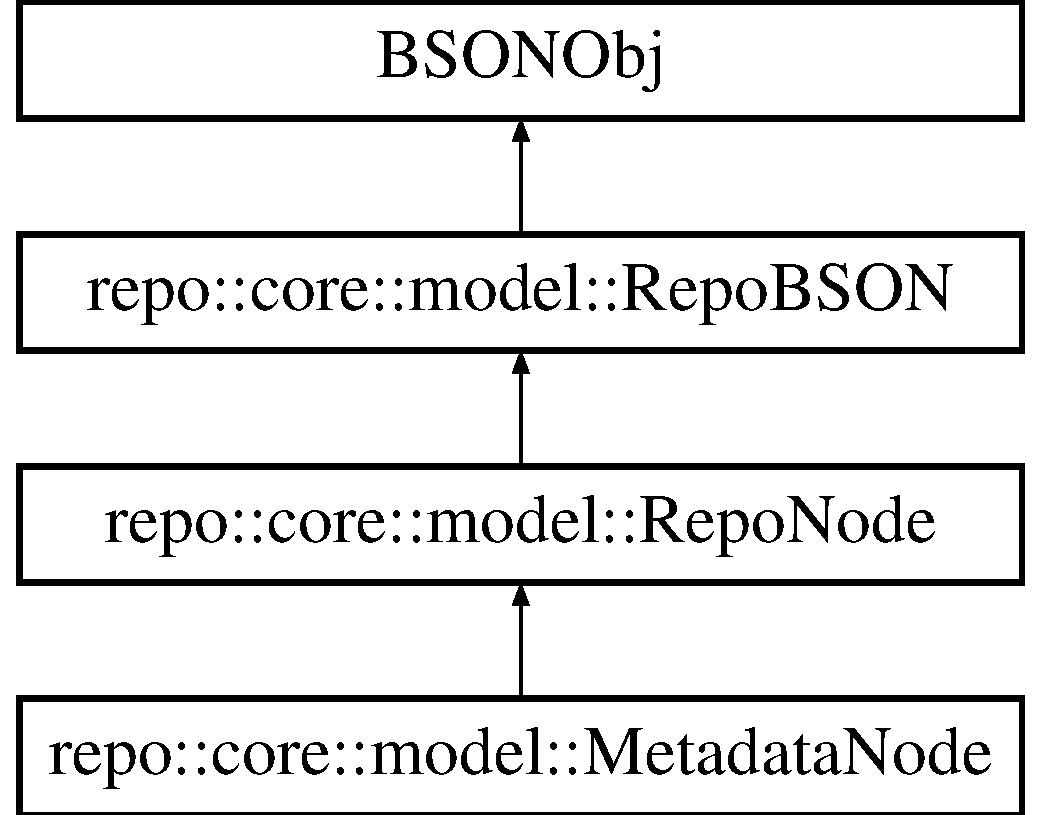
\includegraphics[height=4.000000cm]{classrepo_1_1core_1_1model_1_1_metadata_node}
\end{center}
\end{figure}
\subsection*{Public Member Functions}
\begin{DoxyCompactItemize}
\item 
\hyperlink{classrepo_1_1core_1_1model_1_1_metadata_node_aa5d417f51255811df8a73b2f36edf740}{Metadata\+Node} ()
\item 
\hyperlink{classrepo_1_1core_1_1model_1_1_metadata_node_ad2aca9c43d363cd7a093b5f495b84eef}{Metadata\+Node} (\hyperlink{classrepo_1_1core_1_1model_1_1_repo_b_s_o_n}{Repo\+B\+S\+O\+N} bson, const std\+::unordered\+\_\+map$<$ std\+::string, std\+::pair$<$ std\+::string, std\+::vector$<$ uint8\+\_\+t $>$$>$$>$ \&bin\+Mapping=std\+::unordered\+\_\+map$<$ std\+::string, std\+::pair$<$ std\+::string, std\+::vector$<$ uint8\+\_\+t $>$$>$$>$())
\item 
\hyperlink{classrepo_1_1core_1_1model_1_1_metadata_node_a1d1a2aed0440bee09ab89d5ada8c77cb}{$\sim$\+Metadata\+Node} ()
\item 
virtual std\+::string \hyperlink{classrepo_1_1core_1_1model_1_1_metadata_node_aad51dc79d63495aa6b4b8fd02307786f}{get\+Type} () const 
\item 
virtual Node\+Type \hyperlink{classrepo_1_1core_1_1model_1_1_metadata_node_abc913943e7ce90649aa0d94ef70552ce}{get\+Type\+As\+Enum} () const 
\item 
virtual bool \hyperlink{classrepo_1_1core_1_1model_1_1_metadata_node_a1fd8134ef9585578597b4a8145aebe1d}{s\+Equal} (const \hyperlink{classrepo_1_1core_1_1model_1_1_repo_node}{Repo\+Node} \&other) const 
\item 
\hyperlink{classrepo_1_1core_1_1model_1_1_metadata_node}{Metadata\+Node} \hyperlink{classrepo_1_1core_1_1model_1_1_metadata_node_a515371ea57dc37e9917025d57af9a0f9}{clone\+And\+Add\+Metadata} (const \hyperlink{classrepo_1_1core_1_1model_1_1_repo_b_s_o_n}{Repo\+B\+S\+O\+N} \&metadata) const 
\end{DoxyCompactItemize}
\subsection*{Additional Inherited Members}


\subsection{Constructor \& Destructor Documentation}
\hypertarget{classrepo_1_1core_1_1model_1_1_metadata_node_aa5d417f51255811df8a73b2f36edf740}{}\index{repo\+::core\+::model\+::\+Metadata\+Node@{repo\+::core\+::model\+::\+Metadata\+Node}!Metadata\+Node@{Metadata\+Node}}
\index{Metadata\+Node@{Metadata\+Node}!repo\+::core\+::model\+::\+Metadata\+Node@{repo\+::core\+::model\+::\+Metadata\+Node}}
\subsubsection[{Metadata\+Node}]{\setlength{\rightskip}{0pt plus 5cm}Metadata\+Node\+::\+Metadata\+Node (
\begin{DoxyParamCaption}
{}
\end{DoxyParamCaption}
)}\label{classrepo_1_1core_1_1model_1_1_metadata_node_aa5d417f51255811df8a73b2f36edf740}
Default constructor \hypertarget{classrepo_1_1core_1_1model_1_1_metadata_node_ad2aca9c43d363cd7a093b5f495b84eef}{}\index{repo\+::core\+::model\+::\+Metadata\+Node@{repo\+::core\+::model\+::\+Metadata\+Node}!Metadata\+Node@{Metadata\+Node}}
\index{Metadata\+Node@{Metadata\+Node}!repo\+::core\+::model\+::\+Metadata\+Node@{repo\+::core\+::model\+::\+Metadata\+Node}}
\subsubsection[{Metadata\+Node}]{\setlength{\rightskip}{0pt plus 5cm}Metadata\+Node\+::\+Metadata\+Node (
\begin{DoxyParamCaption}
\item[{{\bf Repo\+B\+S\+O\+N}}]{bson, }
\item[{const std\+::unordered\+\_\+map$<$ std\+::string, std\+::pair$<$ std\+::string, std\+::vector$<$ uint8\+\_\+t $>$$>$$>$ \&}]{bin\+Mapping = {\ttfamily std\+:\+:unordered\+\_\+map$<$std\+:\+:string,~std\+:\+:pair$<$std\+:\+:string,~std\+:\+:vector$<$uint8\+\_\+t$>$$>$$>$()}}
\end{DoxyParamCaption}
)}\label{classrepo_1_1core_1_1model_1_1_metadata_node_ad2aca9c43d363cd7a093b5f495b84eef}
Construct a \hyperlink{classrepo_1_1core_1_1model_1_1_metadata_node}{Metadata\+Node} from a \hyperlink{classrepo_1_1core_1_1model_1_1_repo_b_s_o_n}{Repo\+B\+S\+O\+N} object 
\begin{DoxyParams}{Parameters}
{\em \hyperlink{classrepo_1_1core_1_1model_1_1_repo_b_s_o_n}{Repo\+B\+S\+O\+N}} & object \\
\hline
\end{DoxyParams}
\hypertarget{classrepo_1_1core_1_1model_1_1_metadata_node_a1d1a2aed0440bee09ab89d5ada8c77cb}{}\index{repo\+::core\+::model\+::\+Metadata\+Node@{repo\+::core\+::model\+::\+Metadata\+Node}!````~Metadata\+Node@{$\sim$\+Metadata\+Node}}
\index{````~Metadata\+Node@{$\sim$\+Metadata\+Node}!repo\+::core\+::model\+::\+Metadata\+Node@{repo\+::core\+::model\+::\+Metadata\+Node}}
\subsubsection[{$\sim$\+Metadata\+Node}]{\setlength{\rightskip}{0pt plus 5cm}Metadata\+Node\+::$\sim$\+Metadata\+Node (
\begin{DoxyParamCaption}
{}
\end{DoxyParamCaption}
)}\label{classrepo_1_1core_1_1model_1_1_metadata_node_a1d1a2aed0440bee09ab89d5ada8c77cb}
Default deconstructor 

\subsection{Member Function Documentation}
\hypertarget{classrepo_1_1core_1_1model_1_1_metadata_node_a515371ea57dc37e9917025d57af9a0f9}{}\index{repo\+::core\+::model\+::\+Metadata\+Node@{repo\+::core\+::model\+::\+Metadata\+Node}!clone\+And\+Add\+Metadata@{clone\+And\+Add\+Metadata}}
\index{clone\+And\+Add\+Metadata@{clone\+And\+Add\+Metadata}!repo\+::core\+::model\+::\+Metadata\+Node@{repo\+::core\+::model\+::\+Metadata\+Node}}
\subsubsection[{clone\+And\+Add\+Metadata}]{\setlength{\rightskip}{0pt plus 5cm}{\bf Metadata\+Node} Metadata\+Node\+::clone\+And\+Add\+Metadata (
\begin{DoxyParamCaption}
\item[{const {\bf Repo\+B\+S\+O\+N} \&}]{metadata}
\end{DoxyParamCaption}
) const}\label{classrepo_1_1core_1_1model_1_1_metadata_node_a515371ea57dc37e9917025d57af9a0f9}
Append the given metadata to the list of currently existing metadata 
\begin{DoxyParams}{Parameters}
{\em metadata} & the metadata to add \\
\hline
\end{DoxyParams}
\begin{DoxyReturn}{Returns}
returns a cloned version with updated metadata 
\end{DoxyReturn}
\hypertarget{classrepo_1_1core_1_1model_1_1_metadata_node_aad51dc79d63495aa6b4b8fd02307786f}{}\index{repo\+::core\+::model\+::\+Metadata\+Node@{repo\+::core\+::model\+::\+Metadata\+Node}!get\+Type@{get\+Type}}
\index{get\+Type@{get\+Type}!repo\+::core\+::model\+::\+Metadata\+Node@{repo\+::core\+::model\+::\+Metadata\+Node}}
\subsubsection[{get\+Type}]{\setlength{\rightskip}{0pt plus 5cm}virtual std\+::string repo\+::core\+::model\+::\+Metadata\+Node\+::get\+Type (
\begin{DoxyParamCaption}
{}
\end{DoxyParamCaption}
) const\hspace{0.3cm}{\ttfamily [inline]}, {\ttfamily [virtual]}}\label{classrepo_1_1core_1_1model_1_1_metadata_node_aad51dc79d63495aa6b4b8fd02307786f}
Get the type of node \begin{DoxyReturn}{Returns}
returns the type as a string 
\end{DoxyReturn}


Reimplemented from \hyperlink{classrepo_1_1core_1_1model_1_1_repo_node_a4380ba349235b5d9b13b41e41975805e}{repo\+::core\+::model\+::\+Repo\+Node}.

\hypertarget{classrepo_1_1core_1_1model_1_1_metadata_node_abc913943e7ce90649aa0d94ef70552ce}{}\index{repo\+::core\+::model\+::\+Metadata\+Node@{repo\+::core\+::model\+::\+Metadata\+Node}!get\+Type\+As\+Enum@{get\+Type\+As\+Enum}}
\index{get\+Type\+As\+Enum@{get\+Type\+As\+Enum}!repo\+::core\+::model\+::\+Metadata\+Node@{repo\+::core\+::model\+::\+Metadata\+Node}}
\subsubsection[{get\+Type\+As\+Enum}]{\setlength{\rightskip}{0pt plus 5cm}virtual Node\+Type repo\+::core\+::model\+::\+Metadata\+Node\+::get\+Type\+As\+Enum (
\begin{DoxyParamCaption}
{}
\end{DoxyParamCaption}
) const\hspace{0.3cm}{\ttfamily [inline]}, {\ttfamily [virtual]}}\label{classrepo_1_1core_1_1model_1_1_metadata_node_abc913943e7ce90649aa0d94ef70552ce}
Get the type of node as an enum \begin{DoxyReturn}{Returns}
returns type as enum. 
\end{DoxyReturn}


Reimplemented from \hyperlink{classrepo_1_1core_1_1model_1_1_repo_node_ad8d5295248dc9beb0b91efb2ce3b61f4}{repo\+::core\+::model\+::\+Repo\+Node}.

\hypertarget{classrepo_1_1core_1_1model_1_1_metadata_node_a1fd8134ef9585578597b4a8145aebe1d}{}\index{repo\+::core\+::model\+::\+Metadata\+Node@{repo\+::core\+::model\+::\+Metadata\+Node}!s\+Equal@{s\+Equal}}
\index{s\+Equal@{s\+Equal}!repo\+::core\+::model\+::\+Metadata\+Node@{repo\+::core\+::model\+::\+Metadata\+Node}}
\subsubsection[{s\+Equal}]{\setlength{\rightskip}{0pt plus 5cm}bool Metadata\+Node\+::s\+Equal (
\begin{DoxyParamCaption}
\item[{const {\bf Repo\+Node} \&}]{other}
\end{DoxyParamCaption}
) const\hspace{0.3cm}{\ttfamily [virtual]}}\label{classrepo_1_1core_1_1model_1_1_metadata_node_a1fd8134ef9585578597b4a8145aebe1d}
Check if the node is semantically equal to another Different node should have a different interpretation of what this means. 
\begin{DoxyParams}{Parameters}
{\em other} & node to compare with \\
\hline
{\em returns} & true if equal, false otherwise \\
\hline
\end{DoxyParams}


Reimplemented from \hyperlink{classrepo_1_1core_1_1model_1_1_repo_node_a7c98830a876ee6516587a8f07c7015a5}{repo\+::core\+::model\+::\+Repo\+Node}.



The documentation for this class was generated from the following files\+:\begin{DoxyCompactItemize}
\item 
C\+:/\+Users/\+Carmen/3\+D Repo/\+Repo/3drepobouncer/bouncer/src/repo/core/model/bson/repo\+\_\+node\+\_\+metadata.\+h\item 
C\+:/\+Users/\+Carmen/3\+D Repo/\+Repo/3drepobouncer/bouncer/src/repo/core/model/bson/repo\+\_\+node\+\_\+metadata.\+cpp\end{DoxyCompactItemize}

\hypertarget{classrepo_1_1manipulator_1_1modelconvertor_1_1_model_import_config}{}\section{repo\+:\+:manipulator\+:\+:modelconvertor\+:\+:Model\+Import\+Config Class Reference}
\label{classrepo_1_1manipulator_1_1modelconvertor_1_1_model_import_config}\index{repo\+::manipulator\+::modelconvertor\+::\+Model\+Import\+Config@{repo\+::manipulator\+::modelconvertor\+::\+Model\+Import\+Config}}
\subsection*{Public Member Functions}
\begin{DoxyCompactItemize}
\item 
\hypertarget{classrepo_1_1manipulator_1_1modelconvertor_1_1_model_import_config_a8fddc7e979da71e7feb86363aca76b8e}{}{\bfseries Model\+Import\+Config} (const std\+::string \&config\+File=std\+::string())\label{classrepo_1_1manipulator_1_1modelconvertor_1_1_model_import_config_a8fddc7e979da71e7feb86363aca76b8e}

\item 
virtual bool \hyperlink{classrepo_1_1manipulator_1_1modelconvertor_1_1_model_import_config_abbed1400132285df488e3d49bd5c6a64}{get\+Calculate\+Tangent\+Space} () const 
\item 
virtual float \hyperlink{classrepo_1_1manipulator_1_1modelconvertor_1_1_model_import_config_af787824e4a1737233f74d16ec26bfa9c}{get\+Calculate\+Tangent\+Space\+Max\+Smoothing\+Angle} () const 
\item 
virtual bool \hyperlink{classrepo_1_1manipulator_1_1modelconvertor_1_1_model_import_config_a272769fa5299f0b877256cbb9f182ee0}{get\+Convert\+To\+U\+V\+Coordinates} () const 
\item 
virtual bool \hyperlink{classrepo_1_1manipulator_1_1modelconvertor_1_1_model_import_config_a2ec24b0921862f273025d4421c153c5b}{get\+Degenerates\+To\+Points\+Lines} () const 
\item 
virtual bool \hyperlink{classrepo_1_1manipulator_1_1modelconvertor_1_1_model_import_config_a58d4c2ec483c9886b9ee872211210af8}{get\+Debone} () const 
\item 
virtual float \hyperlink{classrepo_1_1manipulator_1_1modelconvertor_1_1_model_import_config_a7c062c8cbc8574c57f3ffb3ad4b533d9}{get\+Debone\+Threshold} () const 
\item 
virtual bool \hyperlink{classrepo_1_1manipulator_1_1modelconvertor_1_1_model_import_config_ac992c3d0ad11d304bc2a3474bc213754}{get\+Debone\+Only\+If\+All} () const 
\item 
virtual bool \hyperlink{classrepo_1_1manipulator_1_1modelconvertor_1_1_model_import_config_ab14b8ef0f5b2cfec9da90fa254de2133}{get\+Find\+Instances} () const 
\item 
virtual bool \hyperlink{classrepo_1_1manipulator_1_1modelconvertor_1_1_model_import_config_a0d18d6f7c1c3963defa9a45dc2f30db0}{get\+Find\+Invalid\+Data} () const 
\item 
virtual float \hyperlink{classrepo_1_1manipulator_1_1modelconvertor_1_1_model_import_config_ad7ac71713603d1552fc88770e6ed242e}{get\+Find\+Invalid\+Data\+Animation\+Accuracy} () const 
\item 
virtual bool \hyperlink{classrepo_1_1manipulator_1_1modelconvertor_1_1_model_import_config_aa38d7052ee4e0d3af449bdfe729a3afb}{get\+Fix\+Infacing\+Normals} () const 
\item 
virtual bool \hyperlink{classrepo_1_1manipulator_1_1modelconvertor_1_1_model_import_config_a71f86ead55f59f035bec9db32f3aaad0}{get\+Flip\+U\+V\+Coordinates} () const 
\item 
virtual bool \hyperlink{classrepo_1_1manipulator_1_1modelconvertor_1_1_model_import_config_ae2e3b6f3ebfee43e4cc240ef67b6351d}{get\+Flip\+Winding\+Order} () const 
\item 
virtual bool \hyperlink{classrepo_1_1manipulator_1_1modelconvertor_1_1_model_import_config_ad2b6ae83b8a7b8436434869c7fb0d67f}{get\+Generate\+Normals} () const 
\item 
virtual bool \hyperlink{classrepo_1_1manipulator_1_1modelconvertor_1_1_model_import_config_a1e850f706c8ac8b5d9ccacf826756608}{get\+Generate\+Normals\+Flat} () const 
\item 
virtual bool \hyperlink{classrepo_1_1manipulator_1_1modelconvertor_1_1_model_import_config_a53077150e077cc0e4c5bdab11ae57aed}{get\+Generate\+Normals\+Smooth} () const 
\item 
virtual float \hyperlink{classrepo_1_1manipulator_1_1modelconvertor_1_1_model_import_config_aa1e98eaa61a0dc57b262f817bdbc955d}{get\+Generate\+Normals\+Smooth\+Crease\+Angle} () const 
\item 
virtual bool \hyperlink{classrepo_1_1manipulator_1_1modelconvertor_1_1_model_import_config_a01a23d98f545d49052cb4c7432a023fa}{get\+Improve\+Cache\+Locality} () const 
\item 
virtual int \hyperlink{classrepo_1_1manipulator_1_1modelconvertor_1_1_model_import_config_a82d3be19e4c19c95d3562d38d1f245e2}{get\+Improve\+Cache\+Locality\+Vertex\+Cache\+Size} () const 
\item 
virtual bool \hyperlink{classrepo_1_1manipulator_1_1modelconvertor_1_1_model_import_config_aeea89891250d475d64a17765ca8cfda7}{get\+Join\+Identical\+Vertices} () const 
\item 
virtual bool \hyperlink{classrepo_1_1manipulator_1_1modelconvertor_1_1_model_import_config_a15513acb116999ad96b1df1a219f69b9}{get\+Limit\+Bone\+Weights} () const 
\item 
virtual int \hyperlink{classrepo_1_1manipulator_1_1modelconvertor_1_1_model_import_config_a8da86e9887abb758c1b47f5a73490bdf}{get\+Limit\+Bone\+Weights\+Max\+Weight} () const 
\item 
virtual bool \hyperlink{classrepo_1_1manipulator_1_1modelconvertor_1_1_model_import_config_a1fe954cff7d3cc354799516ea19c7ff9}{get\+Make\+Left\+Handed} () const 
\item 
virtual bool \hyperlink{classrepo_1_1manipulator_1_1modelconvertor_1_1_model_import_config_a1e5aed8fd20fe2301ec095865c1c7741}{get\+Optimize\+Meshes} () const 
\item 
virtual bool \hyperlink{classrepo_1_1manipulator_1_1modelconvertor_1_1_model_import_config_a36e8e23ee5a4df2930bf87a0ecb3285d}{get\+Pre\+Transform\+U\+V\+Coordinates} () const 
\item 
virtual bool \hyperlink{classrepo_1_1manipulator_1_1modelconvertor_1_1_model_import_config_a47cb364503eb52629f4c1ee5d5570c26}{get\+Pre\+Transform\+Vertices} () const 
\item 
virtual bool \hyperlink{classrepo_1_1manipulator_1_1modelconvertor_1_1_model_import_config_a3e52a8dc5fa531c35a7997f5499a9cd5}{get\+Pre\+Transform\+Vertices\+Normalize} () const 
\item 
virtual bool \hyperlink{classrepo_1_1manipulator_1_1modelconvertor_1_1_model_import_config_a358ca62515e827b393469da01aae1907}{get\+Remove\+Components} () const 
\item 
virtual bool \hyperlink{classrepo_1_1manipulator_1_1modelconvertor_1_1_model_import_config_acbadab83f14e2b6cb988ae7291813e5d}{get\+Remove\+Components\+Animations} () const 
\item 
virtual bool \hyperlink{classrepo_1_1manipulator_1_1modelconvertor_1_1_model_import_config_a90c71460b0985dc56f4d046eb3f6a9dd}{get\+Remove\+Components\+Bi\+Tangents} () const 
\item 
virtual bool \hyperlink{classrepo_1_1manipulator_1_1modelconvertor_1_1_model_import_config_ac518489da50adf4177bb684235fccda2}{get\+Remove\+Components\+Bone\+Weights} () const 
\item 
virtual bool \hyperlink{classrepo_1_1manipulator_1_1modelconvertor_1_1_model_import_config_a1f1173ef019bce5edfaa52de986e1c32}{get\+Remove\+Components\+Cameras} () const 
\item 
virtual bool \hyperlink{classrepo_1_1manipulator_1_1modelconvertor_1_1_model_import_config_a68b3189a1038fceb5b9f85adca7cea68}{get\+Remove\+Components\+Colors} () const 
\item 
virtual bool \hyperlink{classrepo_1_1manipulator_1_1modelconvertor_1_1_model_import_config_ab83c82e10b04b7d5a8c44c13587d7c86}{get\+Remove\+Components\+Lights} () const 
\item 
virtual bool \hyperlink{classrepo_1_1manipulator_1_1modelconvertor_1_1_model_import_config_ae40e06e6e33c0e6004aa3817cd2775df}{get\+Remove\+Components\+Materials} () const 
\item 
virtual bool \hyperlink{classrepo_1_1manipulator_1_1modelconvertor_1_1_model_import_config_a4b8206abd580c42a1351ffd706d4554f}{get\+Remove\+Components\+Meshes} () const 
\item 
virtual bool \hyperlink{classrepo_1_1manipulator_1_1modelconvertor_1_1_model_import_config_a87395abe2a643c66e4dfe3766086d734}{get\+Remove\+Components\+Normals} () const 
\item 
virtual bool \hyperlink{classrepo_1_1manipulator_1_1modelconvertor_1_1_model_import_config_ac0eff0b8fed6e841c234752214cd578d}{get\+Remove\+Components\+Textures} () const 
\item 
virtual bool \hyperlink{classrepo_1_1manipulator_1_1modelconvertor_1_1_model_import_config_af554b2f1e7fda4d0735054140bc84055}{get\+Remove\+Components\+Texture\+Coordinates} () const 
\item 
virtual bool \hyperlink{classrepo_1_1manipulator_1_1modelconvertor_1_1_model_import_config_abb64793a0284558594e64d0d334a1524}{get\+Remove\+Redundant\+Materials} () const 
\item 
virtual std\+::string \hyperlink{classrepo_1_1manipulator_1_1modelconvertor_1_1_model_import_config_a421717d85170235741c84882fc7fa7ea}{get\+Remove\+Redundant\+Materials\+Skip} () const 
\item 
virtual bool \hyperlink{classrepo_1_1manipulator_1_1modelconvertor_1_1_model_import_config_a36c914e41a2e2da3802af667ea0e7afd}{get\+Remove\+Redundant\+Nodes} () const 
\item 
virtual std\+::string \hyperlink{classrepo_1_1manipulator_1_1modelconvertor_1_1_model_import_config_aca67b2ec7898b55bf312598dd778f366}{get\+Remove\+Redundant\+Nodes\+Skip} () const 
\item 
\hypertarget{classrepo_1_1manipulator_1_1modelconvertor_1_1_model_import_config_a6ba075be40eee6ee300b359ca24017b9}{}virtual bool {\bfseries get\+Skip\+I\+F\+C\+Space\+Representation} () const \label{classrepo_1_1manipulator_1_1modelconvertor_1_1_model_import_config_a6ba075be40eee6ee300b359ca24017b9}

\item 
virtual bool \hyperlink{classrepo_1_1manipulator_1_1modelconvertor_1_1_model_import_config_afa5a790eef9c738bf4cb1facd5bd187d}{get\+Sort\+And\+Remove} () const 
\item 
virtual bool \hyperlink{classrepo_1_1manipulator_1_1modelconvertor_1_1_model_import_config_a4fdc5bd7e139c6b8eb08ed5e05100dae}{get\+Sort\+And\+Remove\+Lines} () const 
\item 
virtual bool \hyperlink{classrepo_1_1manipulator_1_1modelconvertor_1_1_model_import_config_a9baa502ef59aff4d587587d70aef8ddb}{get\+Sort\+And\+Remove\+Points} () const 
\item 
virtual bool \hyperlink{classrepo_1_1manipulator_1_1modelconvertor_1_1_model_import_config_ad787431a2bddbb771ce471732aff24e6}{get\+Sort\+And\+Remove\+Polygons} () const 
\item 
virtual bool \hyperlink{classrepo_1_1manipulator_1_1modelconvertor_1_1_model_import_config_ac7998c1c9af1d593be702670630799ad}{get\+Sort\+And\+Remove\+Triangles} () const 
\item 
virtual bool \hyperlink{classrepo_1_1manipulator_1_1modelconvertor_1_1_model_import_config_a934f64b93300a406890d4dcd0e381117}{get\+Split\+By\+Bone\+Count} () const 
\item 
virtual int \hyperlink{classrepo_1_1manipulator_1_1modelconvertor_1_1_model_import_config_a259bb22eb7d32fb98292a0cc7d0d459c}{get\+Split\+By\+Bone\+Count\+Max\+Bones} () const 
\item 
virtual bool \hyperlink{classrepo_1_1manipulator_1_1modelconvertor_1_1_model_import_config_ae5433b44a2803d6df0dc03611255b895}{get\+Split\+Large\+Meshes} () const 
\item 
virtual int \hyperlink{classrepo_1_1manipulator_1_1modelconvertor_1_1_model_import_config_a24c2d57baf2dbcaea7d406c6a197a703}{get\+Split\+Large\+Meshes\+Triangle\+Limit} () const 
\item 
virtual int \hyperlink{classrepo_1_1manipulator_1_1modelconvertor_1_1_model_import_config_acbc9aa1654b823398c478c88b659ab91}{get\+Split\+Large\+Meshes\+Vertex\+Limit} () const 
\item 
virtual bool \hyperlink{classrepo_1_1manipulator_1_1modelconvertor_1_1_model_import_config_a27dac7c3842f90153c970a522fddea1e}{get\+Triangulate} () const 
\item 
virtual bool \hyperlink{classrepo_1_1manipulator_1_1modelconvertor_1_1_model_import_config_acbdc61bf3a1204b85826f4cca4867ced}{get\+Validate\+Data\+Structures} () const 
\item 
virtual void \hyperlink{classrepo_1_1manipulator_1_1modelconvertor_1_1_model_import_config_ac455657cd5edd144eaf9dcb09102b454}{set\+Calculate\+Tangent\+Space} (bool on)
\begin{DoxyCompactList}\small\item\em Sets the calculate tangent space to settings. \end{DoxyCompactList}\item 
\hypertarget{classrepo_1_1manipulator_1_1modelconvertor_1_1_model_import_config_adbf3ed127e6f943cfea572f1e4665564}{}virtual void {\bfseries set\+Calculate\+Tangent\+Space\+Max\+Smoothing\+Angle} (float angle)\label{classrepo_1_1manipulator_1_1modelconvertor_1_1_model_import_config_adbf3ed127e6f943cfea572f1e4665564}

\item 
\hypertarget{classrepo_1_1manipulator_1_1modelconvertor_1_1_model_import_config_a727eef45aac92dd9b113fd90ab1f51f5}{}virtual void \hyperlink{classrepo_1_1manipulator_1_1modelconvertor_1_1_model_import_config_a727eef45aac92dd9b113fd90ab1f51f5}{set\+Convert\+To\+U\+V\+Coordinates} (bool on)\label{classrepo_1_1manipulator_1_1modelconvertor_1_1_model_import_config_a727eef45aac92dd9b113fd90ab1f51f5}

\begin{DoxyCompactList}\small\item\em Sets the convert to U\+V coordinates to settings. \end{DoxyCompactList}\item 
\hypertarget{classrepo_1_1manipulator_1_1modelconvertor_1_1_model_import_config_ab058a8b1765a41295891b12c71ef6e9f}{}virtual void \hyperlink{classrepo_1_1manipulator_1_1modelconvertor_1_1_model_import_config_ab058a8b1765a41295891b12c71ef6e9f}{set\+Degenerates\+To\+Points\+Lines} (bool on)\label{classrepo_1_1manipulator_1_1modelconvertor_1_1_model_import_config_ab058a8b1765a41295891b12c71ef6e9f}

\begin{DoxyCompactList}\small\item\em Sets the degenerates to points and lines to settings. \end{DoxyCompactList}\item 
\hypertarget{classrepo_1_1manipulator_1_1modelconvertor_1_1_model_import_config_a647cfa99fdbbf8669e8ae58184d66d99}{}virtual void \hyperlink{classrepo_1_1manipulator_1_1modelconvertor_1_1_model_import_config_a647cfa99fdbbf8669e8ae58184d66d99}{set\+Debone} (bool on)\label{classrepo_1_1manipulator_1_1modelconvertor_1_1_model_import_config_a647cfa99fdbbf8669e8ae58184d66d99}

\begin{DoxyCompactList}\small\item\em Sets the debone to settings. \end{DoxyCompactList}\item 
\hypertarget{classrepo_1_1manipulator_1_1modelconvertor_1_1_model_import_config_acd06831c0d6196698229de6b8314d05b}{}virtual void \hyperlink{classrepo_1_1manipulator_1_1modelconvertor_1_1_model_import_config_acd06831c0d6196698229de6b8314d05b}{set\+Debone\+Threshold} (float t)\label{classrepo_1_1manipulator_1_1modelconvertor_1_1_model_import_config_acd06831c0d6196698229de6b8314d05b}

\begin{DoxyCompactList}\small\item\em Sets the debone threshold to settings. \end{DoxyCompactList}\item 
\hypertarget{classrepo_1_1manipulator_1_1modelconvertor_1_1_model_import_config_adddadad6342b5bdf308efd70ca67dcdc}{}virtual void {\bfseries set\+Debone\+Only\+If\+All} (bool on)\label{classrepo_1_1manipulator_1_1modelconvertor_1_1_model_import_config_adddadad6342b5bdf308efd70ca67dcdc}

\item 
\hypertarget{classrepo_1_1manipulator_1_1modelconvertor_1_1_model_import_config_a76f4554949b2e6ba691a920bebe32e7d}{}virtual void {\bfseries set\+Find\+Instances} (bool on)\label{classrepo_1_1manipulator_1_1modelconvertor_1_1_model_import_config_a76f4554949b2e6ba691a920bebe32e7d}

\item 
\hypertarget{classrepo_1_1manipulator_1_1modelconvertor_1_1_model_import_config_a26d975fd0e755182811d9a5daa75771d}{}virtual void {\bfseries set\+Find\+Invalid\+Data} (bool on)\label{classrepo_1_1manipulator_1_1modelconvertor_1_1_model_import_config_a26d975fd0e755182811d9a5daa75771d}

\item 
\hypertarget{classrepo_1_1manipulator_1_1modelconvertor_1_1_model_import_config_afe19ebde000a5a864b1ce1641131c8f6}{}virtual void {\bfseries set\+Find\+Invalid\+Data\+Animation\+Accuracy} (float f)\label{classrepo_1_1manipulator_1_1modelconvertor_1_1_model_import_config_afe19ebde000a5a864b1ce1641131c8f6}

\item 
\hypertarget{classrepo_1_1manipulator_1_1modelconvertor_1_1_model_import_config_a91d03b0359c1d1e22f9cfa145083b72d}{}virtual void {\bfseries set\+Fix\+Infacing\+Normals} (bool on)\label{classrepo_1_1manipulator_1_1modelconvertor_1_1_model_import_config_a91d03b0359c1d1e22f9cfa145083b72d}

\item 
\hypertarget{classrepo_1_1manipulator_1_1modelconvertor_1_1_model_import_config_a509b29f46bf6f3912137c99d60aec2b5}{}virtual void {\bfseries set\+Flip\+U\+V\+Coordinates} (bool on)\label{classrepo_1_1manipulator_1_1modelconvertor_1_1_model_import_config_a509b29f46bf6f3912137c99d60aec2b5}

\item 
\hypertarget{classrepo_1_1manipulator_1_1modelconvertor_1_1_model_import_config_a0750e7b0d0cda09803c57b7e94af0787}{}virtual void {\bfseries set\+Flip\+Winding\+Order} (bool on)\label{classrepo_1_1manipulator_1_1modelconvertor_1_1_model_import_config_a0750e7b0d0cda09803c57b7e94af0787}

\item 
\hypertarget{classrepo_1_1manipulator_1_1modelconvertor_1_1_model_import_config_abbd3cce9ebdf1ecc9b30dc81a0bb7825}{}virtual void {\bfseries set\+Generate\+Normals} (bool on)\label{classrepo_1_1manipulator_1_1modelconvertor_1_1_model_import_config_abbd3cce9ebdf1ecc9b30dc81a0bb7825}

\item 
\hypertarget{classrepo_1_1manipulator_1_1modelconvertor_1_1_model_import_config_a2dc21fcbd35e63c79b55cb801aa97dac}{}virtual void {\bfseries set\+Generate\+Normals\+Flat} (bool on)\label{classrepo_1_1manipulator_1_1modelconvertor_1_1_model_import_config_a2dc21fcbd35e63c79b55cb801aa97dac}

\item 
\hypertarget{classrepo_1_1manipulator_1_1modelconvertor_1_1_model_import_config_ab8f554422b8367b43d62201a7dbe45f5}{}virtual void {\bfseries set\+Generate\+Normals\+Smooth} (bool on)\label{classrepo_1_1manipulator_1_1modelconvertor_1_1_model_import_config_ab8f554422b8367b43d62201a7dbe45f5}

\item 
\hypertarget{classrepo_1_1manipulator_1_1modelconvertor_1_1_model_import_config_ac1407713bcf291b1baa1a42238eba7ee}{}virtual void {\bfseries set\+Generate\+Normals\+Smooth\+Crease\+Angle} (float f)\label{classrepo_1_1manipulator_1_1modelconvertor_1_1_model_import_config_ac1407713bcf291b1baa1a42238eba7ee}

\item 
\hypertarget{classrepo_1_1manipulator_1_1modelconvertor_1_1_model_import_config_ad5c3a442e1581660c077ce56d2bcaa21}{}virtual void {\bfseries set\+Improve\+Cache\+Locality} (bool on)\label{classrepo_1_1manipulator_1_1modelconvertor_1_1_model_import_config_ad5c3a442e1581660c077ce56d2bcaa21}

\item 
\hypertarget{classrepo_1_1manipulator_1_1modelconvertor_1_1_model_import_config_aac4033203d8f39f565fc86560c25e729}{}virtual void {\bfseries set\+Improve\+Cache\+Locality\+Cache\+Size} (int vertex\+Count)\label{classrepo_1_1manipulator_1_1modelconvertor_1_1_model_import_config_aac4033203d8f39f565fc86560c25e729}

\item 
\hypertarget{classrepo_1_1manipulator_1_1modelconvertor_1_1_model_import_config_a4262dd0e48277ac42371a6f2f03fdca1}{}virtual void {\bfseries set\+Join\+Identical\+Vertices} (bool on)\label{classrepo_1_1manipulator_1_1modelconvertor_1_1_model_import_config_a4262dd0e48277ac42371a6f2f03fdca1}

\item 
\hypertarget{classrepo_1_1manipulator_1_1modelconvertor_1_1_model_import_config_a33bfa71fa50ca6d5c4548542e34c6bff}{}virtual void {\bfseries set\+Limit\+Bone\+Weights} (bool on)\label{classrepo_1_1manipulator_1_1modelconvertor_1_1_model_import_config_a33bfa71fa50ca6d5c4548542e34c6bff}

\item 
\hypertarget{classrepo_1_1manipulator_1_1modelconvertor_1_1_model_import_config_a8d90b57b5836257ea1b7f3b28390cac3}{}virtual void {\bfseries set\+Limit\+Bone\+Weights\+Max\+Weights} (int i)\label{classrepo_1_1manipulator_1_1modelconvertor_1_1_model_import_config_a8d90b57b5836257ea1b7f3b28390cac3}

\item 
\hypertarget{classrepo_1_1manipulator_1_1modelconvertor_1_1_model_import_config_a5716bae668b977413b11216424f7cb38}{}virtual void {\bfseries set\+Make\+Left\+Handed} (bool on)\label{classrepo_1_1manipulator_1_1modelconvertor_1_1_model_import_config_a5716bae668b977413b11216424f7cb38}

\item 
\hypertarget{classrepo_1_1manipulator_1_1modelconvertor_1_1_model_import_config_a2cd1f454d88d766af8b0efbcef0cf6dc}{}virtual void {\bfseries set\+Optimize\+Meshes} (bool on)\label{classrepo_1_1manipulator_1_1modelconvertor_1_1_model_import_config_a2cd1f454d88d766af8b0efbcef0cf6dc}

\item 
\hypertarget{classrepo_1_1manipulator_1_1modelconvertor_1_1_model_import_config_a4851e77d18ba2b541e47a0a77029fadc}{}virtual void {\bfseries set\+Pre\+Transform\+U\+V\+Coordinates} (bool on)\label{classrepo_1_1manipulator_1_1modelconvertor_1_1_model_import_config_a4851e77d18ba2b541e47a0a77029fadc}

\item 
\hypertarget{classrepo_1_1manipulator_1_1modelconvertor_1_1_model_import_config_a306be2eff28d78f3faabeece088d77f0}{}virtual void {\bfseries set\+Pre\+Transform\+Vertices} (bool on)\label{classrepo_1_1manipulator_1_1modelconvertor_1_1_model_import_config_a306be2eff28d78f3faabeece088d77f0}

\item 
\hypertarget{classrepo_1_1manipulator_1_1modelconvertor_1_1_model_import_config_a4844abb2dd4d8521258297c09826bef7}{}virtual void {\bfseries set\+Pre\+Transfor\+Vertices\+Normalize} (bool on)\label{classrepo_1_1manipulator_1_1modelconvertor_1_1_model_import_config_a4844abb2dd4d8521258297c09826bef7}

\item 
\hypertarget{classrepo_1_1manipulator_1_1modelconvertor_1_1_model_import_config_ac6a5e5680c325b3570a39b1c4d086f27}{}virtual void {\bfseries set\+Remove\+Components} (bool on)\label{classrepo_1_1manipulator_1_1modelconvertor_1_1_model_import_config_ac6a5e5680c325b3570a39b1c4d086f27}

\item 
\hypertarget{classrepo_1_1manipulator_1_1modelconvertor_1_1_model_import_config_a49c02cf59ff5dfed621164b64219c81c}{}virtual void {\bfseries set\+Remove\+Components\+Animations} (bool on)\label{classrepo_1_1manipulator_1_1modelconvertor_1_1_model_import_config_a49c02cf59ff5dfed621164b64219c81c}

\item 
\hypertarget{classrepo_1_1manipulator_1_1modelconvertor_1_1_model_import_config_aeada200fd73540170bfa8e20cba55ffa}{}virtual void {\bfseries set\+Remove\+Components\+Bi\+Tangents} (bool on)\label{classrepo_1_1manipulator_1_1modelconvertor_1_1_model_import_config_aeada200fd73540170bfa8e20cba55ffa}

\item 
\hypertarget{classrepo_1_1manipulator_1_1modelconvertor_1_1_model_import_config_ab438ed3da03ac48779926fcf88d0a58e}{}virtual void {\bfseries set\+Remove\+Components\+Bone\+Weights} (bool on)\label{classrepo_1_1manipulator_1_1modelconvertor_1_1_model_import_config_ab438ed3da03ac48779926fcf88d0a58e}

\item 
\hypertarget{classrepo_1_1manipulator_1_1modelconvertor_1_1_model_import_config_a364f149efd243e01560c2a14e5f96bbe}{}virtual void {\bfseries set\+Remove\+Components\+Cameras} (bool on)\label{classrepo_1_1manipulator_1_1modelconvertor_1_1_model_import_config_a364f149efd243e01560c2a14e5f96bbe}

\item 
\hypertarget{classrepo_1_1manipulator_1_1modelconvertor_1_1_model_import_config_acb950efbde022b73e52ddba01a650f5f}{}virtual void {\bfseries set\+Remove\+Components\+Colors} (bool on)\label{classrepo_1_1manipulator_1_1modelconvertor_1_1_model_import_config_acb950efbde022b73e52ddba01a650f5f}

\item 
\hypertarget{classrepo_1_1manipulator_1_1modelconvertor_1_1_model_import_config_a5c47a081936100c6dcab1208d2d8775b}{}virtual void {\bfseries set\+Remove\+Components\+Lights} (bool on)\label{classrepo_1_1manipulator_1_1modelconvertor_1_1_model_import_config_a5c47a081936100c6dcab1208d2d8775b}

\item 
\hypertarget{classrepo_1_1manipulator_1_1modelconvertor_1_1_model_import_config_ab696bedadffe52508a67ca91e80fe755}{}virtual void {\bfseries set\+Remove\+Components\+Materials} (bool on)\label{classrepo_1_1manipulator_1_1modelconvertor_1_1_model_import_config_ab696bedadffe52508a67ca91e80fe755}

\item 
\hypertarget{classrepo_1_1manipulator_1_1modelconvertor_1_1_model_import_config_a2545f8ae827096f532590caccc3be3b3}{}virtual void {\bfseries set\+Remove\+Components\+Meshes} (bool on)\label{classrepo_1_1manipulator_1_1modelconvertor_1_1_model_import_config_a2545f8ae827096f532590caccc3be3b3}

\item 
\hypertarget{classrepo_1_1manipulator_1_1modelconvertor_1_1_model_import_config_ae07bb7d7258e77adeea46ad402b15e26}{}virtual void {\bfseries set\+Remove\+Components\+Normals} (bool on)\label{classrepo_1_1manipulator_1_1modelconvertor_1_1_model_import_config_ae07bb7d7258e77adeea46ad402b15e26}

\item 
\hypertarget{classrepo_1_1manipulator_1_1modelconvertor_1_1_model_import_config_af89faf307eb83482b7c036af097018c9}{}virtual void {\bfseries set\+Remove\+Components\+Textures} (bool on)\label{classrepo_1_1manipulator_1_1modelconvertor_1_1_model_import_config_af89faf307eb83482b7c036af097018c9}

\item 
\hypertarget{classrepo_1_1manipulator_1_1modelconvertor_1_1_model_import_config_a37f95e14387e2cb09987db80bcc4d133}{}virtual void {\bfseries set\+Remove\+Components\+Texture\+Coordinates} (bool on)\label{classrepo_1_1manipulator_1_1modelconvertor_1_1_model_import_config_a37f95e14387e2cb09987db80bcc4d133}

\item 
\hypertarget{classrepo_1_1manipulator_1_1modelconvertor_1_1_model_import_config_ab35dff5a9496dbab95a494f79ced76a1}{}virtual void {\bfseries set\+Remove\+Redundant\+Materials} (bool on)\label{classrepo_1_1manipulator_1_1modelconvertor_1_1_model_import_config_ab35dff5a9496dbab95a494f79ced76a1}

\item 
\hypertarget{classrepo_1_1manipulator_1_1modelconvertor_1_1_model_import_config_a8320ed35d8e0333fee9d29fae6087675}{}virtual void {\bfseries set\+Remove\+Redundant\+Materials\+Skip} (const std\+::string \&skip)\label{classrepo_1_1manipulator_1_1modelconvertor_1_1_model_import_config_a8320ed35d8e0333fee9d29fae6087675}

\item 
\hypertarget{classrepo_1_1manipulator_1_1modelconvertor_1_1_model_import_config_a61d64fa91aacc6aec165fd7fd0142270}{}virtual void {\bfseries set\+Remove\+Redundant\+Nodes} (bool on)\label{classrepo_1_1manipulator_1_1modelconvertor_1_1_model_import_config_a61d64fa91aacc6aec165fd7fd0142270}

\item 
\hypertarget{classrepo_1_1manipulator_1_1modelconvertor_1_1_model_import_config_a12e2674ca6a53f15466a0fe452e79e91}{}virtual void {\bfseries set\+Remove\+Redundant\+Nodes\+Skip} (const std\+::string \&skip)\label{classrepo_1_1manipulator_1_1modelconvertor_1_1_model_import_config_a12e2674ca6a53f15466a0fe452e79e91}

\item 
\hypertarget{classrepo_1_1manipulator_1_1modelconvertor_1_1_model_import_config_afecc9f546c66e6f15e0096c6d9470a14}{}virtual void {\bfseries get\+Skip\+I\+F\+C\+Space\+Representation} (const bool \&skip)\label{classrepo_1_1manipulator_1_1modelconvertor_1_1_model_import_config_afecc9f546c66e6f15e0096c6d9470a14}

\item 
\hypertarget{classrepo_1_1manipulator_1_1modelconvertor_1_1_model_import_config_ac3a28a7485a6cf2bed6674854697deea}{}virtual void {\bfseries set\+Sort\+And\+Remove} (bool on)\label{classrepo_1_1manipulator_1_1modelconvertor_1_1_model_import_config_ac3a28a7485a6cf2bed6674854697deea}

\item 
\hypertarget{classrepo_1_1manipulator_1_1modelconvertor_1_1_model_import_config_a51eff792ed22f2a820ef888bfb1e52b9}{}virtual void {\bfseries set\+Sort\+And\+Remove\+Lines} (bool on)\label{classrepo_1_1manipulator_1_1modelconvertor_1_1_model_import_config_a51eff792ed22f2a820ef888bfb1e52b9}

\item 
\hypertarget{classrepo_1_1manipulator_1_1modelconvertor_1_1_model_import_config_aad0e696973b75bf9ea662c1ff716f455}{}virtual void {\bfseries set\+Sort\+And\+Remove\+Points} (bool on)\label{classrepo_1_1manipulator_1_1modelconvertor_1_1_model_import_config_aad0e696973b75bf9ea662c1ff716f455}

\item 
\hypertarget{classrepo_1_1manipulator_1_1modelconvertor_1_1_model_import_config_a844eface85f5a5300c5c8484dc9e399e}{}virtual void {\bfseries set\+Sort\+And\+Remove\+Polygons} (bool on)\label{classrepo_1_1manipulator_1_1modelconvertor_1_1_model_import_config_a844eface85f5a5300c5c8484dc9e399e}

\item 
\hypertarget{classrepo_1_1manipulator_1_1modelconvertor_1_1_model_import_config_a3d4b0f2ab05dafb91cd73c93ad395f06}{}virtual void {\bfseries set\+Sort\+And\+Remove\+Triangles} (bool on)\label{classrepo_1_1manipulator_1_1modelconvertor_1_1_model_import_config_a3d4b0f2ab05dafb91cd73c93ad395f06}

\item 
\hypertarget{classrepo_1_1manipulator_1_1modelconvertor_1_1_model_import_config_a68e8069ca1b1bdef325c14348b59cf20}{}virtual void {\bfseries set\+Split\+By\+Bone\+Count} (bool on)\label{classrepo_1_1manipulator_1_1modelconvertor_1_1_model_import_config_a68e8069ca1b1bdef325c14348b59cf20}

\item 
\hypertarget{classrepo_1_1manipulator_1_1modelconvertor_1_1_model_import_config_ac7175074012f491a23e01dd26719e22d}{}virtual void {\bfseries set\+Split\+By\+Bone\+Count\+Max\+Bones} (int max)\label{classrepo_1_1manipulator_1_1modelconvertor_1_1_model_import_config_ac7175074012f491a23e01dd26719e22d}

\item 
\hypertarget{classrepo_1_1manipulator_1_1modelconvertor_1_1_model_import_config_aa54c8324e3ab66f75b91aaaa5bf8635d}{}virtual void {\bfseries set\+Split\+Large\+Meshes} (bool on)\label{classrepo_1_1manipulator_1_1modelconvertor_1_1_model_import_config_aa54c8324e3ab66f75b91aaaa5bf8635d}

\item 
\hypertarget{classrepo_1_1manipulator_1_1modelconvertor_1_1_model_import_config_a8fb74b5c8b832488c93e70687e209826}{}virtual void {\bfseries set\+Split\+Large\+Meshes\+Triangle\+Limit} (int limit)\label{classrepo_1_1manipulator_1_1modelconvertor_1_1_model_import_config_a8fb74b5c8b832488c93e70687e209826}

\item 
\hypertarget{classrepo_1_1manipulator_1_1modelconvertor_1_1_model_import_config_ab1c7da74a50bd8087a45b9c6850a479a}{}virtual void {\bfseries set\+Split\+Large\+Meshes\+Vertex\+Limit} (int limit)\label{classrepo_1_1manipulator_1_1modelconvertor_1_1_model_import_config_ab1c7da74a50bd8087a45b9c6850a479a}

\item 
\hypertarget{classrepo_1_1manipulator_1_1modelconvertor_1_1_model_import_config_ae300ca5c00f14907ba3a5ac041864b7b}{}virtual void {\bfseries set\+Triangulate} (bool on)\label{classrepo_1_1manipulator_1_1modelconvertor_1_1_model_import_config_ae300ca5c00f14907ba3a5ac041864b7b}

\item 
\hypertarget{classrepo_1_1manipulator_1_1modelconvertor_1_1_model_import_config_aa3cd72a04646715c92baa5642b4b4e51}{}virtual void {\bfseries set\+Validate\+Data\+Structures} (bool on)\label{classrepo_1_1manipulator_1_1modelconvertor_1_1_model_import_config_aa3cd72a04646715c92baa5642b4b4e51}

\end{DoxyCompactItemize}
\subsection*{Protected Member Functions}
\begin{DoxyCompactItemize}
\item 
void \hyperlink{classrepo_1_1manipulator_1_1modelconvertor_1_1_model_import_config_ad185cdda25389ab799d2c21f09d96c19}{reset} ()
\item 
void \hyperlink{classrepo_1_1manipulator_1_1modelconvertor_1_1_model_import_config_ab293453a220b87ff8f1d2c87d20404b8}{read\+Config} (std\+::ifstream \&conf)
\item 
\hypertarget{classrepo_1_1manipulator_1_1modelconvertor_1_1_model_import_config_a47c109f402daf3e2fc6e01f0c3632c32}{}void {\bfseries set\+Value} (std\+::string label, bool value)\label{classrepo_1_1manipulator_1_1modelconvertor_1_1_model_import_config_a47c109f402daf3e2fc6e01f0c3632c32}

\item 
\hypertarget{classrepo_1_1manipulator_1_1modelconvertor_1_1_model_import_config_a43b7997f63cf92595fd86f81bb65bfb5}{}void {\bfseries set\+Value} (std\+::string label, int32\+\_\+t value)\label{classrepo_1_1manipulator_1_1modelconvertor_1_1_model_import_config_a43b7997f63cf92595fd86f81bb65bfb5}

\item 
\hypertarget{classrepo_1_1manipulator_1_1modelconvertor_1_1_model_import_config_ab49fef1d68b2edb159bb675ad7a5c9d0}{}void {\bfseries set\+Value} (std\+::string label, float value)\label{classrepo_1_1manipulator_1_1modelconvertor_1_1_model_import_config_ab49fef1d68b2edb159bb675ad7a5c9d0}

\item 
\hypertarget{classrepo_1_1manipulator_1_1modelconvertor_1_1_model_import_config_adefc71f79e860dceddf7e11f3f8532df}{}void {\bfseries set\+Value} (std\+::string label, std\+::string value)\label{classrepo_1_1manipulator_1_1modelconvertor_1_1_model_import_config_adefc71f79e860dceddf7e11f3f8532df}

\end{DoxyCompactItemize}
\subsection*{Protected Attributes}
\begin{DoxyCompactItemize}
\item 
\hypertarget{classrepo_1_1manipulator_1_1modelconvertor_1_1_model_import_config_a23d095a344f1b498c25b116e49d5bef5}{}std\+::map$<$ std\+::string, bool $>$ {\bfseries bool\+Settings}\label{classrepo_1_1manipulator_1_1modelconvertor_1_1_model_import_config_a23d095a344f1b498c25b116e49d5bef5}

\item 
\hypertarget{classrepo_1_1manipulator_1_1modelconvertor_1_1_model_import_config_a9870b6020b0f484031f4883f433bec16}{}std\+::map$<$ std\+::string, int32\+\_\+t $>$ {\bfseries int\+Settings}\label{classrepo_1_1manipulator_1_1modelconvertor_1_1_model_import_config_a9870b6020b0f484031f4883f433bec16}

\item 
\hypertarget{classrepo_1_1manipulator_1_1modelconvertor_1_1_model_import_config_a5112f7722fdb1562e287b23e9104430c}{}std\+::map$<$ std\+::string, float $>$ {\bfseries float\+Settings}\label{classrepo_1_1manipulator_1_1modelconvertor_1_1_model_import_config_a5112f7722fdb1562e287b23e9104430c}

\item 
\hypertarget{classrepo_1_1manipulator_1_1modelconvertor_1_1_model_import_config_a95b4afb72dc7a172855d1ade993bccb2}{}std\+::map$<$ std\+::string, std\+::string $>$ {\bfseries string\+Settings}\label{classrepo_1_1manipulator_1_1modelconvertor_1_1_model_import_config_a95b4afb72dc7a172855d1ade993bccb2}

\end{DoxyCompactItemize}
\subsection*{Static Protected Attributes}
\begin{DoxyCompactItemize}
\item 
\hypertarget{classrepo_1_1manipulator_1_1modelconvertor_1_1_model_import_config_a141e61b65d0896d215463acb4a33cb42}{}static const std\+::string {\bfseries C\+A\+L\+C\+U\+L\+A\+T\+E\+\_\+\+T\+A\+N\+G\+E\+N\+T\+\_\+\+S\+P\+A\+C\+E} = \char`\"{}calculate\+Tangent\+Space\char`\"{}\label{classrepo_1_1manipulator_1_1modelconvertor_1_1_model_import_config_a141e61b65d0896d215463acb4a33cb42}

\item 
\hypertarget{classrepo_1_1manipulator_1_1modelconvertor_1_1_model_import_config_a7251d2f069376102f0d7d7ef5ecac72a}{}static const std\+::string {\bfseries C\+A\+L\+C\+U\+L\+A\+T\+E\+\_\+\+T\+A\+N\+G\+E\+N\+T\+\_\+\+S\+P\+A\+C\+E\+\_\+\+M\+A\+X\+\_\+\+S\+M\+O\+O\+T\+H\+I\+N\+G\+\_\+\+A\+N\+G\+L\+E} = \char`\"{}calculate\+Tangent\+Space\+Max\+Smoothing\+Angle\char`\"{}\label{classrepo_1_1manipulator_1_1modelconvertor_1_1_model_import_config_a7251d2f069376102f0d7d7ef5ecac72a}

\item 
\hypertarget{classrepo_1_1manipulator_1_1modelconvertor_1_1_model_import_config_adee6e7c8adddb7713334fa74161985ad}{}static const std\+::string {\bfseries C\+O\+N\+V\+E\+R\+T\+\_\+\+T\+O\+\_\+\+U\+V\+\_\+\+C\+O\+O\+R\+D\+I\+N\+A\+T\+E\+S} = \char`\"{}convert\+To\+U\+V\+Coordinates\char`\"{}\label{classrepo_1_1manipulator_1_1modelconvertor_1_1_model_import_config_adee6e7c8adddb7713334fa74161985ad}

\item 
\hypertarget{classrepo_1_1manipulator_1_1modelconvertor_1_1_model_import_config_a18e164f211203288e79dcaf46d697d7a}{}static const std\+::string {\bfseries D\+E\+G\+E\+N\+E\+R\+A\+T\+E\+S\+\_\+\+T\+O\+\_\+\+P\+O\+I\+N\+T\+S\+\_\+\+L\+I\+N\+E\+S} = \char`\"{}degenerates\+To\+Poinst\+Lines\char`\"{}\label{classrepo_1_1manipulator_1_1modelconvertor_1_1_model_import_config_a18e164f211203288e79dcaf46d697d7a}

\item 
\hypertarget{classrepo_1_1manipulator_1_1modelconvertor_1_1_model_import_config_adea8d96a90d0d2026a9d8e2a2543cf03}{}static const std\+::string {\bfseries D\+E\+B\+O\+N\+E} = \char`\"{}debone\char`\"{}\label{classrepo_1_1manipulator_1_1modelconvertor_1_1_model_import_config_adea8d96a90d0d2026a9d8e2a2543cf03}

\item 
\hypertarget{classrepo_1_1manipulator_1_1modelconvertor_1_1_model_import_config_a2a234d780f860e8a030c50379bede907}{}static const std\+::string {\bfseries D\+E\+B\+O\+N\+E\+\_\+\+T\+H\+R\+E\+S\+H\+O\+L\+D} = \char`\"{}debone\+Threshold\char`\"{}\label{classrepo_1_1manipulator_1_1modelconvertor_1_1_model_import_config_a2a234d780f860e8a030c50379bede907}

\item 
\hypertarget{classrepo_1_1manipulator_1_1modelconvertor_1_1_model_import_config_a940a4a19793113db0b79552529665f30}{}static const std\+::string {\bfseries D\+E\+B\+O\+N\+E\+\_\+\+O\+N\+L\+Y\+\_\+\+I\+F\+\_\+\+A\+L\+L} = \char`\"{}debone\+Only\+If\+All\char`\"{}\label{classrepo_1_1manipulator_1_1modelconvertor_1_1_model_import_config_a940a4a19793113db0b79552529665f30}

\item 
\hypertarget{classrepo_1_1manipulator_1_1modelconvertor_1_1_model_import_config_a5051583e215c14706bbdf2294c4460ba}{}static const std\+::string {\bfseries F\+I\+N\+D\+\_\+\+I\+N\+S\+T\+A\+N\+C\+E\+S} = \char`\"{}find\+Instances\char`\"{}\label{classrepo_1_1manipulator_1_1modelconvertor_1_1_model_import_config_a5051583e215c14706bbdf2294c4460ba}

\item 
\hypertarget{classrepo_1_1manipulator_1_1modelconvertor_1_1_model_import_config_aa009d5d58b94d3a8c4641fba11df436f}{}static const std\+::string {\bfseries F\+I\+N\+D\+\_\+\+I\+N\+A\+V\+L\+I\+D\+\_\+\+D\+A\+T\+A} = \char`\"{}find\+Invalid\+Data\char`\"{}\label{classrepo_1_1manipulator_1_1modelconvertor_1_1_model_import_config_aa009d5d58b94d3a8c4641fba11df436f}

\item 
\hypertarget{classrepo_1_1manipulator_1_1modelconvertor_1_1_model_import_config_a70498c5e3b6d7f1924111ac26a66f402}{}static const std\+::string {\bfseries F\+I\+N\+D\+\_\+\+I\+N\+A\+V\+L\+I\+D\+\_\+\+D\+A\+T\+A\+\_\+\+A\+N\+I\+M\+A\+T\+I\+O\+N\+\_\+\+A\+C\+C\+U\+R\+A\+C\+Y} = \char`\"{}find\+Invalid\+Data\+Animation\+Accuracy\char`\"{}\label{classrepo_1_1manipulator_1_1modelconvertor_1_1_model_import_config_a70498c5e3b6d7f1924111ac26a66f402}

\item 
\hypertarget{classrepo_1_1manipulator_1_1modelconvertor_1_1_model_import_config_a2e4328217c13cf74749bdaac08a75863}{}static const std\+::string {\bfseries F\+I\+X\+\_\+\+I\+N\+F\+A\+C\+I\+N\+G\+\_\+\+N\+O\+R\+M\+A\+L\+S} = \char`\"{}fix\+Infacing\+Normals\char`\"{}\label{classrepo_1_1manipulator_1_1modelconvertor_1_1_model_import_config_a2e4328217c13cf74749bdaac08a75863}

\item 
\hypertarget{classrepo_1_1manipulator_1_1modelconvertor_1_1_model_import_config_a196cb90d3ef7d8b7800152ded97c73b5}{}static const std\+::string {\bfseries F\+L\+I\+P\+\_\+\+U\+V\+\_\+\+C\+O\+O\+R\+D\+I\+N\+A\+T\+E\+S} = \char`\"{}flip\+U\+V\+Coordinates\char`\"{}\label{classrepo_1_1manipulator_1_1modelconvertor_1_1_model_import_config_a196cb90d3ef7d8b7800152ded97c73b5}

\item 
\hypertarget{classrepo_1_1manipulator_1_1modelconvertor_1_1_model_import_config_a36c34f96c5ad4d81dbb9f70ef358306b}{}static const std\+::string {\bfseries F\+L\+I\+P\+\_\+\+W\+I\+N\+D\+I\+N\+G\+\_\+\+O\+R\+D\+E\+R} = \char`\"{}flip\+Winding\+Order\char`\"{}\label{classrepo_1_1manipulator_1_1modelconvertor_1_1_model_import_config_a36c34f96c5ad4d81dbb9f70ef358306b}

\item 
\hypertarget{classrepo_1_1manipulator_1_1modelconvertor_1_1_model_import_config_a567bf55463d94abaa42a6f131acf0b97}{}static const std\+::string {\bfseries G\+E\+N\+E\+R\+A\+T\+E\+\_\+\+N\+O\+R\+M\+A\+L\+S} = \char`\"{}generate\+Normals\char`\"{}\label{classrepo_1_1manipulator_1_1modelconvertor_1_1_model_import_config_a567bf55463d94abaa42a6f131acf0b97}

\item 
\hypertarget{classrepo_1_1manipulator_1_1modelconvertor_1_1_model_import_config_ab97f2e7d9c21dda9568267ce91a981b5}{}static const std\+::string {\bfseries G\+E\+N\+E\+R\+A\+T\+E\+\_\+\+N\+O\+R\+M\+A\+L\+S\+\_\+\+F\+L\+A\+T} = \char`\"{}generate\+Normals\+Flat\char`\"{}\label{classrepo_1_1manipulator_1_1modelconvertor_1_1_model_import_config_ab97f2e7d9c21dda9568267ce91a981b5}

\item 
\hypertarget{classrepo_1_1manipulator_1_1modelconvertor_1_1_model_import_config_a8b5e901666b55fea2241afb14793d0f1}{}static const std\+::string {\bfseries G\+E\+N\+E\+R\+A\+T\+E\+\_\+\+N\+O\+R\+M\+A\+L\+S\+\_\+\+S\+M\+O\+O\+T\+H} = \char`\"{}generate\+Normals\+Smooth\char`\"{}\label{classrepo_1_1manipulator_1_1modelconvertor_1_1_model_import_config_a8b5e901666b55fea2241afb14793d0f1}

\item 
\hypertarget{classrepo_1_1manipulator_1_1modelconvertor_1_1_model_import_config_af7ed06294f90863aa714a1289ec4c3d8}{}static const std\+::string {\bfseries G\+E\+N\+E\+R\+A\+T\+E\+\_\+\+N\+O\+R\+M\+A\+L\+S\+\_\+\+S\+M\+O\+O\+T\+H\+\_\+\+C\+R\+E\+A\+S\+E\+\_\+\+A\+N\+G\+L\+E} = \char`\"{}generate\+Normals\+Smooth\+Crease\+Angle\char`\"{}\label{classrepo_1_1manipulator_1_1modelconvertor_1_1_model_import_config_af7ed06294f90863aa714a1289ec4c3d8}

\item 
\hypertarget{classrepo_1_1manipulator_1_1modelconvertor_1_1_model_import_config_a0b78b393e90c4867aecab0dfcd88d3cf}{}static const std\+::string {\bfseries I\+F\+C\+\_\+\+S\+K\+I\+P\+\_\+\+S\+P\+A\+C\+E\+\_\+\+R\+E\+P\+R\+E\+S\+E\+N\+T\+A\+T\+I\+O\+N\+S} = \char`\"{}skip\+I\+F\+C\+Space\+Representations\char`\"{}\label{classrepo_1_1manipulator_1_1modelconvertor_1_1_model_import_config_a0b78b393e90c4867aecab0dfcd88d3cf}

\item 
\hypertarget{classrepo_1_1manipulator_1_1modelconvertor_1_1_model_import_config_ade39d8c7feb9dfa9c976673ba357e8e2}{}static const std\+::string {\bfseries I\+M\+P\+R\+O\+V\+E\+\_\+\+C\+A\+C\+H\+E\+\_\+\+L\+O\+C\+A\+L\+I\+T\+Y} = \char`\"{}improve\+Cache\+Locality\char`\"{}\label{classrepo_1_1manipulator_1_1modelconvertor_1_1_model_import_config_ade39d8c7feb9dfa9c976673ba357e8e2}

\item 
\hypertarget{classrepo_1_1manipulator_1_1modelconvertor_1_1_model_import_config_a69ab02c4c06040101af573dbd7d691a5}{}static const std\+::string {\bfseries I\+M\+P\+R\+O\+V\+E\+\_\+\+C\+A\+C\+H\+E\+\_\+\+L\+O\+C\+A\+L\+I\+T\+Y\+\_\+\+V\+E\+R\+T\+E\+X\+\_\+\+C\+A\+C\+H\+E\+\_\+\+S\+I\+Z\+E} = \char`\"{}improve\+Cache\+Locality\+Vertex\+Cache\+Size\char`\"{}\label{classrepo_1_1manipulator_1_1modelconvertor_1_1_model_import_config_a69ab02c4c06040101af573dbd7d691a5}

\item 
\hypertarget{classrepo_1_1manipulator_1_1modelconvertor_1_1_model_import_config_a3114a2dfb3903d96490adb1309237445}{}static const std\+::string {\bfseries J\+O\+I\+N\+\_\+\+I\+D\+E\+N\+T\+I\+C\+A\+L\+\_\+\+V\+E\+R\+T\+I\+C\+E\+S} = \char`\"{}join\+Identical\+Vertices\char`\"{}\label{classrepo_1_1manipulator_1_1modelconvertor_1_1_model_import_config_a3114a2dfb3903d96490adb1309237445}

\item 
\hypertarget{classrepo_1_1manipulator_1_1modelconvertor_1_1_model_import_config_a6c4a93a78c559fa12112f0db0f05e0c8}{}static const std\+::string {\bfseries L\+I\+M\+I\+T\+\_\+\+B\+O\+N\+E\+\_\+\+W\+E\+I\+G\+H\+T\+S} = \char`\"{}limit\+Bone\+Weights\char`\"{}\label{classrepo_1_1manipulator_1_1modelconvertor_1_1_model_import_config_a6c4a93a78c559fa12112f0db0f05e0c8}

\item 
\hypertarget{classrepo_1_1manipulator_1_1modelconvertor_1_1_model_import_config_a1adf345e9ebe53d52b9cb9972febf6f5}{}static const std\+::string {\bfseries L\+I\+M\+I\+T\+\_\+\+B\+O\+N\+E\+\_\+\+W\+E\+I\+G\+H\+T\+S\+\_\+\+M\+A\+X\+\_\+\+W\+E\+I\+G\+H\+T\+S} = \char`\"{}limit\+Bone\+Weights\+Max\+Weight\char`\"{}\label{classrepo_1_1manipulator_1_1modelconvertor_1_1_model_import_config_a1adf345e9ebe53d52b9cb9972febf6f5}

\item 
\hypertarget{classrepo_1_1manipulator_1_1modelconvertor_1_1_model_import_config_aecbf71733abfeec8cf733cb9ea1dd6dd}{}static const std\+::string {\bfseries M\+A\+K\+E\+\_\+\+L\+E\+F\+T\+\_\+\+H\+A\+N\+D\+E\+D} = \char`\"{}make\+Left\+Handed\char`\"{}\label{classrepo_1_1manipulator_1_1modelconvertor_1_1_model_import_config_aecbf71733abfeec8cf733cb9ea1dd6dd}

\item 
\hypertarget{classrepo_1_1manipulator_1_1modelconvertor_1_1_model_import_config_a3540510fe29c173d6dec5263067a6786}{}static const std\+::string {\bfseries O\+P\+T\+I\+M\+I\+Z\+E\+\_\+\+M\+E\+S\+H\+E\+S} = \char`\"{}optimize\+Meshes\char`\"{}\label{classrepo_1_1manipulator_1_1modelconvertor_1_1_model_import_config_a3540510fe29c173d6dec5263067a6786}

\item 
\hypertarget{classrepo_1_1manipulator_1_1modelconvertor_1_1_model_import_config_af0b1960d45b341dfa3e335f89db1e534}{}static const std\+::string {\bfseries P\+R\+E\+\_\+\+T\+R\+A\+N\+S\+F\+O\+R\+M\+\_\+\+U\+V\+\_\+\+C\+O\+O\+R\+D\+I\+N\+A\+T\+E\+S} = \char`\"{}pre\+Transform\+U\+V\+Coordinates\char`\"{}\label{classrepo_1_1manipulator_1_1modelconvertor_1_1_model_import_config_af0b1960d45b341dfa3e335f89db1e534}

\item 
\hypertarget{classrepo_1_1manipulator_1_1modelconvertor_1_1_model_import_config_acf7b8e5200c436bb53d35a1e990f25f9}{}static const std\+::string {\bfseries P\+R\+E\+\_\+\+T\+R\+A\+N\+S\+F\+O\+R\+M\+\_\+\+V\+E\+R\+T\+I\+C\+E\+S} = \char`\"{}pre\+Transform\+Vertices\char`\"{}\label{classrepo_1_1manipulator_1_1modelconvertor_1_1_model_import_config_acf7b8e5200c436bb53d35a1e990f25f9}

\item 
\hypertarget{classrepo_1_1manipulator_1_1modelconvertor_1_1_model_import_config_a8a1b93cd1986276bf8e1c490df0f9efa}{}static const std\+::string {\bfseries P\+R\+E\+\_\+\+T\+R\+A\+N\+S\+F\+O\+R\+M\+\_\+\+V\+E\+R\+T\+I\+C\+E\+S\+\_\+\+N\+O\+R\+M\+A\+L\+I\+Z\+E} = \char`\"{}pre\+Transform\+Vertices\+Normalize\char`\"{}\label{classrepo_1_1manipulator_1_1modelconvertor_1_1_model_import_config_a8a1b93cd1986276bf8e1c490df0f9efa}

\item 
\hypertarget{classrepo_1_1manipulator_1_1modelconvertor_1_1_model_import_config_a7cf9984c799cea2cceb74b17f46570d7}{}static const std\+::string {\bfseries R\+E\+M\+O\+V\+E\+\_\+\+C\+O\+M\+P\+O\+N\+E\+N\+T\+S} = \char`\"{}remove\+Components\char`\"{}\label{classrepo_1_1manipulator_1_1modelconvertor_1_1_model_import_config_a7cf9984c799cea2cceb74b17f46570d7}

\item 
\hypertarget{classrepo_1_1manipulator_1_1modelconvertor_1_1_model_import_config_a372589a7a74591e165fad2297908a75a}{}static const std\+::string {\bfseries R\+E\+M\+O\+V\+E\+\_\+\+C\+O\+M\+P\+O\+N\+E\+N\+T\+S\+\_\+\+A\+N\+I\+M\+A\+T\+I\+O\+N\+S} = \char`\"{}remove\+Components\+Animations\char`\"{}\label{classrepo_1_1manipulator_1_1modelconvertor_1_1_model_import_config_a372589a7a74591e165fad2297908a75a}

\item 
\hypertarget{classrepo_1_1manipulator_1_1modelconvertor_1_1_model_import_config_a727a1c9daa3261bb2e4493194d6b07f7}{}static const std\+::string {\bfseries R\+E\+M\+O\+V\+E\+\_\+\+C\+O\+M\+P\+O\+N\+E\+N\+T\+S\+\_\+\+B\+I\+\_\+\+T\+A\+N\+G\+E\+N\+T\+S} = \char`\"{}remove\+Components\+Bi\+Tangents\char`\"{}\label{classrepo_1_1manipulator_1_1modelconvertor_1_1_model_import_config_a727a1c9daa3261bb2e4493194d6b07f7}

\item 
\hypertarget{classrepo_1_1manipulator_1_1modelconvertor_1_1_model_import_config_a5cf1ba914153b6a2e1cf6f9816654e80}{}static const std\+::string {\bfseries R\+E\+M\+O\+V\+E\+\_\+\+C\+O\+M\+P\+O\+N\+E\+N\+T\+S\+\_\+\+B\+O\+N\+E\+\_\+\+W\+E\+I\+G\+H\+T\+S} = \char`\"{}remove\+Components\+Bone\+Weights\char`\"{}\label{classrepo_1_1manipulator_1_1modelconvertor_1_1_model_import_config_a5cf1ba914153b6a2e1cf6f9816654e80}

\item 
\hypertarget{classrepo_1_1manipulator_1_1modelconvertor_1_1_model_import_config_a2ca3bb5d8b7334fa159851473579bc83}{}static const std\+::string {\bfseries R\+E\+M\+O\+V\+E\+\_\+\+C\+O\+M\+P\+O\+N\+E\+N\+T\+S\+\_\+\+C\+A\+M\+E\+R\+A\+S} = \char`\"{}remove\+Components\+Cameras\char`\"{}\label{classrepo_1_1manipulator_1_1modelconvertor_1_1_model_import_config_a2ca3bb5d8b7334fa159851473579bc83}

\item 
\hypertarget{classrepo_1_1manipulator_1_1modelconvertor_1_1_model_import_config_a504471fe2255358d64ffa712bdb3f233}{}static const std\+::string {\bfseries R\+E\+M\+O\+V\+E\+\_\+\+C\+O\+M\+P\+O\+N\+E\+N\+T\+S\+\_\+\+C\+O\+L\+O\+R\+S} = \char`\"{}remove\+Components\+Colors\char`\"{}\label{classrepo_1_1manipulator_1_1modelconvertor_1_1_model_import_config_a504471fe2255358d64ffa712bdb3f233}

\item 
\hypertarget{classrepo_1_1manipulator_1_1modelconvertor_1_1_model_import_config_ad9e150b3cb05fe0e12ec25a2659e6ec2}{}static const std\+::string {\bfseries R\+E\+M\+O\+V\+E\+\_\+\+C\+O\+M\+P\+O\+N\+E\+N\+T\+S\+\_\+\+L\+I\+G\+H\+T\+S} = \char`\"{}remove\+Components\+Lights\char`\"{}\label{classrepo_1_1manipulator_1_1modelconvertor_1_1_model_import_config_ad9e150b3cb05fe0e12ec25a2659e6ec2}

\item 
\hypertarget{classrepo_1_1manipulator_1_1modelconvertor_1_1_model_import_config_abade5c555654ac7ad7866b607fe985ca}{}static const std\+::string {\bfseries R\+E\+M\+O\+V\+E\+\_\+\+C\+O\+M\+P\+O\+N\+E\+N\+T\+S\+\_\+\+M\+A\+T\+E\+R\+I\+A\+L\+S} = \char`\"{}remove\+Components\+Materials\char`\"{}\label{classrepo_1_1manipulator_1_1modelconvertor_1_1_model_import_config_abade5c555654ac7ad7866b607fe985ca}

\item 
\hypertarget{classrepo_1_1manipulator_1_1modelconvertor_1_1_model_import_config_a111eaba9f952d9dd17c258714804b51e}{}static const std\+::string {\bfseries R\+E\+M\+O\+V\+E\+\_\+\+C\+O\+M\+P\+O\+N\+E\+N\+T\+S\+\_\+\+M\+E\+S\+H\+E\+S} = \char`\"{}remove\+Components\+Meshes\char`\"{}\label{classrepo_1_1manipulator_1_1modelconvertor_1_1_model_import_config_a111eaba9f952d9dd17c258714804b51e}

\item 
\hypertarget{classrepo_1_1manipulator_1_1modelconvertor_1_1_model_import_config_a98569e123fd241d1499c41639363e7e8}{}static const std\+::string {\bfseries R\+E\+M\+O\+V\+E\+\_\+\+C\+O\+M\+P\+O\+N\+E\+N\+T\+S\+\_\+\+N\+O\+R\+M\+A\+L\+S} = \char`\"{}remove\+Components\+Normals\char`\"{}\label{classrepo_1_1manipulator_1_1modelconvertor_1_1_model_import_config_a98569e123fd241d1499c41639363e7e8}

\item 
\hypertarget{classrepo_1_1manipulator_1_1modelconvertor_1_1_model_import_config_a53b9d9ce14b3d8aa3b55afb8dc7764d3}{}static const std\+::string {\bfseries R\+E\+M\+O\+V\+E\+\_\+\+C\+O\+M\+P\+O\+N\+E\+N\+T\+S\+\_\+\+T\+E\+X\+T\+U\+R\+E\+S} = \char`\"{}remove\+Components\+Textures\char`\"{}\label{classrepo_1_1manipulator_1_1modelconvertor_1_1_model_import_config_a53b9d9ce14b3d8aa3b55afb8dc7764d3}

\item 
\hypertarget{classrepo_1_1manipulator_1_1modelconvertor_1_1_model_import_config_a8116eec9f891876eca43261dc26ea230}{}static const std\+::string {\bfseries R\+E\+M\+O\+V\+E\+\_\+\+C\+O\+M\+P\+O\+N\+E\+N\+T\+S\+\_\+\+T\+E\+X\+T\+U\+R\+E\+\_\+\+C\+O\+O\+R\+D\+I\+N\+A\+T\+E\+S} = \char`\"{}remove\+Components\+Texture\+Coordinates\char`\"{}\label{classrepo_1_1manipulator_1_1modelconvertor_1_1_model_import_config_a8116eec9f891876eca43261dc26ea230}

\item 
\hypertarget{classrepo_1_1manipulator_1_1modelconvertor_1_1_model_import_config_ac820adb9ac0ca35bcd68aae0d3c2f5c6}{}static const std\+::string {\bfseries R\+E\+M\+O\+V\+E\+\_\+\+R\+E\+D\+U\+N\+D\+A\+N\+T\+\_\+\+M\+A\+T\+E\+R\+I\+A\+L\+S} = \char`\"{}remove\+Redundant\+Materials\char`\"{}\label{classrepo_1_1manipulator_1_1modelconvertor_1_1_model_import_config_ac820adb9ac0ca35bcd68aae0d3c2f5c6}

\item 
\hypertarget{classrepo_1_1manipulator_1_1modelconvertor_1_1_model_import_config_a003b6e0a8d481f1306fc6880129f48cb}{}static const std\+::string {\bfseries R\+E\+M\+O\+V\+E\+\_\+\+R\+E\+D\+U\+N\+D\+A\+N\+T\+\_\+\+M\+A\+T\+E\+R\+I\+A\+L\+S\+\_\+\+S\+K\+I\+P} = \char`\"{}remove\+Redundant\+Materials\+Skip\char`\"{}\label{classrepo_1_1manipulator_1_1modelconvertor_1_1_model_import_config_a003b6e0a8d481f1306fc6880129f48cb}

\item 
\hypertarget{classrepo_1_1manipulator_1_1modelconvertor_1_1_model_import_config_afa1f8291118174a4f3c1d5043fda51c7}{}static const std\+::string {\bfseries R\+E\+M\+O\+V\+E\+\_\+\+R\+E\+D\+U\+N\+D\+A\+N\+T\+\_\+\+N\+O\+D\+E\+S} = \char`\"{}remove\+Redundant\+Nodes\char`\"{}\label{classrepo_1_1manipulator_1_1modelconvertor_1_1_model_import_config_afa1f8291118174a4f3c1d5043fda51c7}

\item 
\hypertarget{classrepo_1_1manipulator_1_1modelconvertor_1_1_model_import_config_a4a6b28358aa662917b2bb10f066ac468}{}static const std\+::string {\bfseries R\+E\+M\+O\+V\+E\+\_\+\+R\+E\+D\+U\+N\+D\+A\+N\+T\+\_\+\+N\+O\+D\+E\+S\+\_\+\+S\+K\+I\+P} = \char`\"{}remove\+Redundant\+Nodes\+Skip\char`\"{}\label{classrepo_1_1manipulator_1_1modelconvertor_1_1_model_import_config_a4a6b28358aa662917b2bb10f066ac468}

\item 
\hypertarget{classrepo_1_1manipulator_1_1modelconvertor_1_1_model_import_config_a888dc28ee93f04bb87050ae2d0c2eb2d}{}static const std\+::string {\bfseries S\+O\+R\+T\+\_\+\+A\+N\+D\+\_\+\+R\+E\+M\+O\+V\+E} = \char`\"{}sort\+And\+Remove\char`\"{}\label{classrepo_1_1manipulator_1_1modelconvertor_1_1_model_import_config_a888dc28ee93f04bb87050ae2d0c2eb2d}

\item 
\hypertarget{classrepo_1_1manipulator_1_1modelconvertor_1_1_model_import_config_a3b7ef0076d667ecf55cb862907e054b4}{}static const std\+::string {\bfseries S\+O\+R\+T\+\_\+\+A\+N\+D\+\_\+\+R\+E\+M\+O\+V\+E\+\_\+\+P\+O\+I\+N\+T\+S} = \char`\"{}sort\+And\+Remove\+Points\char`\"{}\label{classrepo_1_1manipulator_1_1modelconvertor_1_1_model_import_config_a3b7ef0076d667ecf55cb862907e054b4}

\item 
\hypertarget{classrepo_1_1manipulator_1_1modelconvertor_1_1_model_import_config_adb1e96658247b43fb8dd89933b16da1c}{}static const std\+::string {\bfseries S\+O\+R\+T\+\_\+\+A\+N\+D\+\_\+\+R\+E\+M\+O\+V\+E\+\_\+\+L\+I\+N\+E\+S} = \char`\"{}sort\+And\+Remove\+Lines\char`\"{}\label{classrepo_1_1manipulator_1_1modelconvertor_1_1_model_import_config_adb1e96658247b43fb8dd89933b16da1c}

\item 
\hypertarget{classrepo_1_1manipulator_1_1modelconvertor_1_1_model_import_config_abc359b43ad4c6541df7db8f5c5fd9e60}{}static const std\+::string {\bfseries S\+O\+R\+T\+\_\+\+A\+N\+D\+\_\+\+R\+E\+M\+O\+V\+E\+\_\+\+T\+R\+I\+A\+N\+G\+L\+E\+S} = \char`\"{}sort\+And\+Remove\+Triangles\char`\"{}\label{classrepo_1_1manipulator_1_1modelconvertor_1_1_model_import_config_abc359b43ad4c6541df7db8f5c5fd9e60}

\item 
\hypertarget{classrepo_1_1manipulator_1_1modelconvertor_1_1_model_import_config_af198b48edbdda3e881807df0e1ac9f50}{}static const std\+::string {\bfseries S\+O\+R\+T\+\_\+\+A\+N\+D\+\_\+\+R\+E\+M\+O\+V\+E\+\_\+\+P\+O\+L\+Y\+G\+O\+N\+S} = \char`\"{}sort\+And\+Remove\+Polygons\char`\"{}\label{classrepo_1_1manipulator_1_1modelconvertor_1_1_model_import_config_af198b48edbdda3e881807df0e1ac9f50}

\item 
\hypertarget{classrepo_1_1manipulator_1_1modelconvertor_1_1_model_import_config_a65171d535961d7cfe9600e04efc8482e}{}static const std\+::string {\bfseries S\+P\+L\+I\+T\+\_\+\+B\+Y\+\_\+\+B\+O\+N\+E\+\_\+\+C\+O\+U\+N\+T} = \char`\"{}split\+By\+Bone\+Count\char`\"{}\label{classrepo_1_1manipulator_1_1modelconvertor_1_1_model_import_config_a65171d535961d7cfe9600e04efc8482e}

\item 
\hypertarget{classrepo_1_1manipulator_1_1modelconvertor_1_1_model_import_config_ace598dc881841bac5b31d39963258329}{}static const std\+::string {\bfseries S\+P\+L\+I\+T\+\_\+\+B\+Y\+\_\+\+B\+O\+N\+E\+\_\+\+C\+O\+U\+N\+T\+\_\+\+M\+A\+X\+\_\+\+B\+O\+N\+E\+S} = \char`\"{}split\+By\+Bone\+Count\+Max\+Bones\char`\"{}\label{classrepo_1_1manipulator_1_1modelconvertor_1_1_model_import_config_ace598dc881841bac5b31d39963258329}

\item 
\hypertarget{classrepo_1_1manipulator_1_1modelconvertor_1_1_model_import_config_a9c0f0fc500d2c9cf97647ec2114809e3}{}static const std\+::string {\bfseries S\+P\+L\+I\+T\+\_\+\+L\+A\+R\+G\+E\+\_\+\+M\+E\+S\+H\+E\+S} = \char`\"{}split\+Large\+Meshes\char`\"{}\label{classrepo_1_1manipulator_1_1modelconvertor_1_1_model_import_config_a9c0f0fc500d2c9cf97647ec2114809e3}

\item 
\hypertarget{classrepo_1_1manipulator_1_1modelconvertor_1_1_model_import_config_a026a2461e11668cc97bdcd51c85f6578}{}static const std\+::string {\bfseries S\+P\+L\+I\+T\+\_\+\+L\+A\+R\+G\+E\+\_\+\+M\+E\+S\+H\+E\+S\+\_\+\+T\+R\+I\+A\+N\+G\+L\+E\+\_\+\+L\+I\+M\+I\+T} = \char`\"{}split\+Large\+Meshes\+Triangle\+Limit\char`\"{}\label{classrepo_1_1manipulator_1_1modelconvertor_1_1_model_import_config_a026a2461e11668cc97bdcd51c85f6578}

\item 
\hypertarget{classrepo_1_1manipulator_1_1modelconvertor_1_1_model_import_config_a42b5d704d0bd57f1c2cde47ff5d1745e}{}static const std\+::string {\bfseries S\+P\+L\+I\+T\+\_\+\+L\+A\+R\+G\+E\+\_\+\+M\+E\+S\+H\+E\+S\+\_\+\+V\+E\+R\+T\+E\+X\+\_\+\+L\+I\+M\+I\+T} = \char`\"{}split\+Large\+Meshes\+Vertex\+Limit\char`\"{}\label{classrepo_1_1manipulator_1_1modelconvertor_1_1_model_import_config_a42b5d704d0bd57f1c2cde47ff5d1745e}

\item 
\hypertarget{classrepo_1_1manipulator_1_1modelconvertor_1_1_model_import_config_a29172af362b27a47e44df9317489ceed}{}static const std\+::string {\bfseries T\+R\+I\+A\+N\+G\+U\+L\+A\+T\+E} = \char`\"{}triangulate\char`\"{}\label{classrepo_1_1manipulator_1_1modelconvertor_1_1_model_import_config_a29172af362b27a47e44df9317489ceed}

\item 
\hypertarget{classrepo_1_1manipulator_1_1modelconvertor_1_1_model_import_config_a4cb316e06b113877f1197a8c4db3e9f1}{}static const std\+::string {\bfseries V\+A\+L\+I\+D\+A\+T\+E\+\_\+\+D\+A\+T\+A\+\_\+\+S\+T\+R\+U\+C\+T\+U\+R\+E\+S} = \char`\"{}validate\+Data\+Structures\char`\"{}\label{classrepo_1_1manipulator_1_1modelconvertor_1_1_model_import_config_a4cb316e06b113877f1197a8c4db3e9f1}

\end{DoxyCompactItemize}


\subsection{Member Function Documentation}
\hypertarget{classrepo_1_1manipulator_1_1modelconvertor_1_1_model_import_config_abbed1400132285df488e3d49bd5c6a64}{}\index{repo\+::manipulator\+::modelconvertor\+::\+Model\+Import\+Config@{repo\+::manipulator\+::modelconvertor\+::\+Model\+Import\+Config}!get\+Calculate\+Tangent\+Space@{get\+Calculate\+Tangent\+Space}}
\index{get\+Calculate\+Tangent\+Space@{get\+Calculate\+Tangent\+Space}!repo\+::manipulator\+::modelconvertor\+::\+Model\+Import\+Config@{repo\+::manipulator\+::modelconvertor\+::\+Model\+Import\+Config}}
\subsubsection[{get\+Calculate\+Tangent\+Space}]{\setlength{\rightskip}{0pt plus 5cm}virtual bool repo\+::manipulator\+::modelconvertor\+::\+Model\+Import\+Config\+::get\+Calculate\+Tangent\+Space (
\begin{DoxyParamCaption}
{}
\end{DoxyParamCaption}
) const\hspace{0.3cm}{\ttfamily [inline]}, {\ttfamily [virtual]}}\label{classrepo_1_1manipulator_1_1modelconvertor_1_1_model_import_config_abbed1400132285df488e3d49bd5c6a64}
-\/-\/-\/-\/-\/-\/-\/-\/-\/-\/------ Getters -\/-\/-\/-\/-\/-\/-\/-\/-\/-\/-\/-\/-\/-\/-\/-\/-\/-\/-\/------

Returns true if calculate tangent space is checked in settings, false otherwise. Defaults to false. \hypertarget{classrepo_1_1manipulator_1_1modelconvertor_1_1_model_import_config_af787824e4a1737233f74d16ec26bfa9c}{}\index{repo\+::manipulator\+::modelconvertor\+::\+Model\+Import\+Config@{repo\+::manipulator\+::modelconvertor\+::\+Model\+Import\+Config}!get\+Calculate\+Tangent\+Space\+Max\+Smoothing\+Angle@{get\+Calculate\+Tangent\+Space\+Max\+Smoothing\+Angle}}
\index{get\+Calculate\+Tangent\+Space\+Max\+Smoothing\+Angle@{get\+Calculate\+Tangent\+Space\+Max\+Smoothing\+Angle}!repo\+::manipulator\+::modelconvertor\+::\+Model\+Import\+Config@{repo\+::manipulator\+::modelconvertor\+::\+Model\+Import\+Config}}
\subsubsection[{get\+Calculate\+Tangent\+Space\+Max\+Smoothing\+Angle}]{\setlength{\rightskip}{0pt plus 5cm}virtual float repo\+::manipulator\+::modelconvertor\+::\+Model\+Import\+Config\+::get\+Calculate\+Tangent\+Space\+Max\+Smoothing\+Angle (
\begin{DoxyParamCaption}
{}
\end{DoxyParamCaption}
) const\hspace{0.3cm}{\ttfamily [inline]}, {\ttfamily [virtual]}}\label{classrepo_1_1manipulator_1_1modelconvertor_1_1_model_import_config_af787824e4a1737233f74d16ec26bfa9c}
Returns the maximum smoothing angle for calc tangent space. Defaults to 45. \hypertarget{classrepo_1_1manipulator_1_1modelconvertor_1_1_model_import_config_a272769fa5299f0b877256cbb9f182ee0}{}\index{repo\+::manipulator\+::modelconvertor\+::\+Model\+Import\+Config@{repo\+::manipulator\+::modelconvertor\+::\+Model\+Import\+Config}!get\+Convert\+To\+U\+V\+Coordinates@{get\+Convert\+To\+U\+V\+Coordinates}}
\index{get\+Convert\+To\+U\+V\+Coordinates@{get\+Convert\+To\+U\+V\+Coordinates}!repo\+::manipulator\+::modelconvertor\+::\+Model\+Import\+Config@{repo\+::manipulator\+::modelconvertor\+::\+Model\+Import\+Config}}
\subsubsection[{get\+Convert\+To\+U\+V\+Coordinates}]{\setlength{\rightskip}{0pt plus 5cm}virtual bool repo\+::manipulator\+::modelconvertor\+::\+Model\+Import\+Config\+::get\+Convert\+To\+U\+V\+Coordinates (
\begin{DoxyParamCaption}
{}
\end{DoxyParamCaption}
) const\hspace{0.3cm}{\ttfamily [inline]}, {\ttfamily [virtual]}}\label{classrepo_1_1manipulator_1_1modelconvertor_1_1_model_import_config_a272769fa5299f0b877256cbb9f182ee0}
Returns true if convert to U\+V coords is checked in settings, false otherwise. Defaults to false. \hypertarget{classrepo_1_1manipulator_1_1modelconvertor_1_1_model_import_config_a58d4c2ec483c9886b9ee872211210af8}{}\index{repo\+::manipulator\+::modelconvertor\+::\+Model\+Import\+Config@{repo\+::manipulator\+::modelconvertor\+::\+Model\+Import\+Config}!get\+Debone@{get\+Debone}}
\index{get\+Debone@{get\+Debone}!repo\+::manipulator\+::modelconvertor\+::\+Model\+Import\+Config@{repo\+::manipulator\+::modelconvertor\+::\+Model\+Import\+Config}}
\subsubsection[{get\+Debone}]{\setlength{\rightskip}{0pt plus 5cm}virtual bool repo\+::manipulator\+::modelconvertor\+::\+Model\+Import\+Config\+::get\+Debone (
\begin{DoxyParamCaption}
{}
\end{DoxyParamCaption}
) const\hspace{0.3cm}{\ttfamily [inline]}, {\ttfamily [virtual]}}\label{classrepo_1_1manipulator_1_1modelconvertor_1_1_model_import_config_a58d4c2ec483c9886b9ee872211210af8}
Returns true if debone is checked in settings, false otherwise. Defaults to false. \hypertarget{classrepo_1_1manipulator_1_1modelconvertor_1_1_model_import_config_ac992c3d0ad11d304bc2a3474bc213754}{}\index{repo\+::manipulator\+::modelconvertor\+::\+Model\+Import\+Config@{repo\+::manipulator\+::modelconvertor\+::\+Model\+Import\+Config}!get\+Debone\+Only\+If\+All@{get\+Debone\+Only\+If\+All}}
\index{get\+Debone\+Only\+If\+All@{get\+Debone\+Only\+If\+All}!repo\+::manipulator\+::modelconvertor\+::\+Model\+Import\+Config@{repo\+::manipulator\+::modelconvertor\+::\+Model\+Import\+Config}}
\subsubsection[{get\+Debone\+Only\+If\+All}]{\setlength{\rightskip}{0pt plus 5cm}virtual bool repo\+::manipulator\+::modelconvertor\+::\+Model\+Import\+Config\+::get\+Debone\+Only\+If\+All (
\begin{DoxyParamCaption}
{}
\end{DoxyParamCaption}
) const\hspace{0.3cm}{\ttfamily [inline]}, {\ttfamily [virtual]}}\label{classrepo_1_1manipulator_1_1modelconvertor_1_1_model_import_config_ac992c3d0ad11d304bc2a3474bc213754}
Returns true if debone only if all is checked in settings, false otherwise. Defaults to false. \hypertarget{classrepo_1_1manipulator_1_1modelconvertor_1_1_model_import_config_a7c062c8cbc8574c57f3ffb3ad4b533d9}{}\index{repo\+::manipulator\+::modelconvertor\+::\+Model\+Import\+Config@{repo\+::manipulator\+::modelconvertor\+::\+Model\+Import\+Config}!get\+Debone\+Threshold@{get\+Debone\+Threshold}}
\index{get\+Debone\+Threshold@{get\+Debone\+Threshold}!repo\+::manipulator\+::modelconvertor\+::\+Model\+Import\+Config@{repo\+::manipulator\+::modelconvertor\+::\+Model\+Import\+Config}}
\subsubsection[{get\+Debone\+Threshold}]{\setlength{\rightskip}{0pt plus 5cm}virtual float repo\+::manipulator\+::modelconvertor\+::\+Model\+Import\+Config\+::get\+Debone\+Threshold (
\begin{DoxyParamCaption}
{}
\end{DoxyParamCaption}
) const\hspace{0.3cm}{\ttfamily [inline]}, {\ttfamily [virtual]}}\label{classrepo_1_1manipulator_1_1modelconvertor_1_1_model_import_config_a7c062c8cbc8574c57f3ffb3ad4b533d9}
Returns the debone threshold set in settings. Defaults to Assimp\textquotesingle{}s A\+I\+\_\+\+D\+E\+B\+O\+N\+E\+\_\+\+T\+H\+R\+E\+S\+H\+O\+L\+D = 1.\+0f \hypertarget{classrepo_1_1manipulator_1_1modelconvertor_1_1_model_import_config_a2ec24b0921862f273025d4421c153c5b}{}\index{repo\+::manipulator\+::modelconvertor\+::\+Model\+Import\+Config@{repo\+::manipulator\+::modelconvertor\+::\+Model\+Import\+Config}!get\+Degenerates\+To\+Points\+Lines@{get\+Degenerates\+To\+Points\+Lines}}
\index{get\+Degenerates\+To\+Points\+Lines@{get\+Degenerates\+To\+Points\+Lines}!repo\+::manipulator\+::modelconvertor\+::\+Model\+Import\+Config@{repo\+::manipulator\+::modelconvertor\+::\+Model\+Import\+Config}}
\subsubsection[{get\+Degenerates\+To\+Points\+Lines}]{\setlength{\rightskip}{0pt plus 5cm}virtual bool repo\+::manipulator\+::modelconvertor\+::\+Model\+Import\+Config\+::get\+Degenerates\+To\+Points\+Lines (
\begin{DoxyParamCaption}
{}
\end{DoxyParamCaption}
) const\hspace{0.3cm}{\ttfamily [inline]}, {\ttfamily [virtual]}}\label{classrepo_1_1manipulator_1_1modelconvertor_1_1_model_import_config_a2ec24b0921862f273025d4421c153c5b}
Returns true if degenerates to points/lines is checked in settings, false otherwise. Defaults to false. \hypertarget{classrepo_1_1manipulator_1_1modelconvertor_1_1_model_import_config_ab14b8ef0f5b2cfec9da90fa254de2133}{}\index{repo\+::manipulator\+::modelconvertor\+::\+Model\+Import\+Config@{repo\+::manipulator\+::modelconvertor\+::\+Model\+Import\+Config}!get\+Find\+Instances@{get\+Find\+Instances}}
\index{get\+Find\+Instances@{get\+Find\+Instances}!repo\+::manipulator\+::modelconvertor\+::\+Model\+Import\+Config@{repo\+::manipulator\+::modelconvertor\+::\+Model\+Import\+Config}}
\subsubsection[{get\+Find\+Instances}]{\setlength{\rightskip}{0pt plus 5cm}virtual bool repo\+::manipulator\+::modelconvertor\+::\+Model\+Import\+Config\+::get\+Find\+Instances (
\begin{DoxyParamCaption}
{}
\end{DoxyParamCaption}
) const\hspace{0.3cm}{\ttfamily [inline]}, {\ttfamily [virtual]}}\label{classrepo_1_1manipulator_1_1modelconvertor_1_1_model_import_config_ab14b8ef0f5b2cfec9da90fa254de2133}
Returns true if find instances is checked in settings, false otherwise. Defaults to false. \hypertarget{classrepo_1_1manipulator_1_1modelconvertor_1_1_model_import_config_a0d18d6f7c1c3963defa9a45dc2f30db0}{}\index{repo\+::manipulator\+::modelconvertor\+::\+Model\+Import\+Config@{repo\+::manipulator\+::modelconvertor\+::\+Model\+Import\+Config}!get\+Find\+Invalid\+Data@{get\+Find\+Invalid\+Data}}
\index{get\+Find\+Invalid\+Data@{get\+Find\+Invalid\+Data}!repo\+::manipulator\+::modelconvertor\+::\+Model\+Import\+Config@{repo\+::manipulator\+::modelconvertor\+::\+Model\+Import\+Config}}
\subsubsection[{get\+Find\+Invalid\+Data}]{\setlength{\rightskip}{0pt plus 5cm}virtual bool repo\+::manipulator\+::modelconvertor\+::\+Model\+Import\+Config\+::get\+Find\+Invalid\+Data (
\begin{DoxyParamCaption}
{}
\end{DoxyParamCaption}
) const\hspace{0.3cm}{\ttfamily [inline]}, {\ttfamily [virtual]}}\label{classrepo_1_1manipulator_1_1modelconvertor_1_1_model_import_config_a0d18d6f7c1c3963defa9a45dc2f30db0}
Returns true if find invalid data is checked in settings, false otherwise. Defaults to false. \hypertarget{classrepo_1_1manipulator_1_1modelconvertor_1_1_model_import_config_ad7ac71713603d1552fc88770e6ed242e}{}\index{repo\+::manipulator\+::modelconvertor\+::\+Model\+Import\+Config@{repo\+::manipulator\+::modelconvertor\+::\+Model\+Import\+Config}!get\+Find\+Invalid\+Data\+Animation\+Accuracy@{get\+Find\+Invalid\+Data\+Animation\+Accuracy}}
\index{get\+Find\+Invalid\+Data\+Animation\+Accuracy@{get\+Find\+Invalid\+Data\+Animation\+Accuracy}!repo\+::manipulator\+::modelconvertor\+::\+Model\+Import\+Config@{repo\+::manipulator\+::modelconvertor\+::\+Model\+Import\+Config}}
\subsubsection[{get\+Find\+Invalid\+Data\+Animation\+Accuracy}]{\setlength{\rightskip}{0pt plus 5cm}virtual float repo\+::manipulator\+::modelconvertor\+::\+Model\+Import\+Config\+::get\+Find\+Invalid\+Data\+Animation\+Accuracy (
\begin{DoxyParamCaption}
{}
\end{DoxyParamCaption}
) const\hspace{0.3cm}{\ttfamily [inline]}, {\ttfamily [virtual]}}\label{classrepo_1_1manipulator_1_1modelconvertor_1_1_model_import_config_ad7ac71713603d1552fc88770e6ed242e}
Returns the animation accuracy for find invalid data set in settings. Defaults to 0.\+0f == all comparisons are exact. See \href{http://assimp.sourceforge.net/lib_html/config_8h.html#ad223c5e7e63d2937685cc704a181b950}{\tt http\+://assimp.\+sourceforge.\+net/lib\+\_\+html/config\+\_\+8h.\+html\#ad223c5e7e63d2937685cc704a181b950} \hypertarget{classrepo_1_1manipulator_1_1modelconvertor_1_1_model_import_config_aa38d7052ee4e0d3af449bdfe729a3afb}{}\index{repo\+::manipulator\+::modelconvertor\+::\+Model\+Import\+Config@{repo\+::manipulator\+::modelconvertor\+::\+Model\+Import\+Config}!get\+Fix\+Infacing\+Normals@{get\+Fix\+Infacing\+Normals}}
\index{get\+Fix\+Infacing\+Normals@{get\+Fix\+Infacing\+Normals}!repo\+::manipulator\+::modelconvertor\+::\+Model\+Import\+Config@{repo\+::manipulator\+::modelconvertor\+::\+Model\+Import\+Config}}
\subsubsection[{get\+Fix\+Infacing\+Normals}]{\setlength{\rightskip}{0pt plus 5cm}virtual bool repo\+::manipulator\+::modelconvertor\+::\+Model\+Import\+Config\+::get\+Fix\+Infacing\+Normals (
\begin{DoxyParamCaption}
{}
\end{DoxyParamCaption}
) const\hspace{0.3cm}{\ttfamily [inline]}, {\ttfamily [virtual]}}\label{classrepo_1_1manipulator_1_1modelconvertor_1_1_model_import_config_aa38d7052ee4e0d3af449bdfe729a3afb}
Returns true if fix infacing normals is checked in settings, false otherwise. Defaults to false. \hypertarget{classrepo_1_1manipulator_1_1modelconvertor_1_1_model_import_config_a71f86ead55f59f035bec9db32f3aaad0}{}\index{repo\+::manipulator\+::modelconvertor\+::\+Model\+Import\+Config@{repo\+::manipulator\+::modelconvertor\+::\+Model\+Import\+Config}!get\+Flip\+U\+V\+Coordinates@{get\+Flip\+U\+V\+Coordinates}}
\index{get\+Flip\+U\+V\+Coordinates@{get\+Flip\+U\+V\+Coordinates}!repo\+::manipulator\+::modelconvertor\+::\+Model\+Import\+Config@{repo\+::manipulator\+::modelconvertor\+::\+Model\+Import\+Config}}
\subsubsection[{get\+Flip\+U\+V\+Coordinates}]{\setlength{\rightskip}{0pt plus 5cm}virtual bool repo\+::manipulator\+::modelconvertor\+::\+Model\+Import\+Config\+::get\+Flip\+U\+V\+Coordinates (
\begin{DoxyParamCaption}
{}
\end{DoxyParamCaption}
) const\hspace{0.3cm}{\ttfamily [inline]}, {\ttfamily [virtual]}}\label{classrepo_1_1manipulator_1_1modelconvertor_1_1_model_import_config_a71f86ead55f59f035bec9db32f3aaad0}
Returns true if flip U\+V coordinates is checked in settings, false otherwise. Defaults to false. \hypertarget{classrepo_1_1manipulator_1_1modelconvertor_1_1_model_import_config_ae2e3b6f3ebfee43e4cc240ef67b6351d}{}\index{repo\+::manipulator\+::modelconvertor\+::\+Model\+Import\+Config@{repo\+::manipulator\+::modelconvertor\+::\+Model\+Import\+Config}!get\+Flip\+Winding\+Order@{get\+Flip\+Winding\+Order}}
\index{get\+Flip\+Winding\+Order@{get\+Flip\+Winding\+Order}!repo\+::manipulator\+::modelconvertor\+::\+Model\+Import\+Config@{repo\+::manipulator\+::modelconvertor\+::\+Model\+Import\+Config}}
\subsubsection[{get\+Flip\+Winding\+Order}]{\setlength{\rightskip}{0pt plus 5cm}virtual bool repo\+::manipulator\+::modelconvertor\+::\+Model\+Import\+Config\+::get\+Flip\+Winding\+Order (
\begin{DoxyParamCaption}
{}
\end{DoxyParamCaption}
) const\hspace{0.3cm}{\ttfamily [inline]}, {\ttfamily [virtual]}}\label{classrepo_1_1manipulator_1_1modelconvertor_1_1_model_import_config_ae2e3b6f3ebfee43e4cc240ef67b6351d}
Returns true if flip winding order is checked in settings, false otherwise. Defaults to false. \hypertarget{classrepo_1_1manipulator_1_1modelconvertor_1_1_model_import_config_ad2b6ae83b8a7b8436434869c7fb0d67f}{}\index{repo\+::manipulator\+::modelconvertor\+::\+Model\+Import\+Config@{repo\+::manipulator\+::modelconvertor\+::\+Model\+Import\+Config}!get\+Generate\+Normals@{get\+Generate\+Normals}}
\index{get\+Generate\+Normals@{get\+Generate\+Normals}!repo\+::manipulator\+::modelconvertor\+::\+Model\+Import\+Config@{repo\+::manipulator\+::modelconvertor\+::\+Model\+Import\+Config}}
\subsubsection[{get\+Generate\+Normals}]{\setlength{\rightskip}{0pt plus 5cm}virtual bool repo\+::manipulator\+::modelconvertor\+::\+Model\+Import\+Config\+::get\+Generate\+Normals (
\begin{DoxyParamCaption}
{}
\end{DoxyParamCaption}
) const\hspace{0.3cm}{\ttfamily [inline]}, {\ttfamily [virtual]}}\label{classrepo_1_1manipulator_1_1modelconvertor_1_1_model_import_config_ad2b6ae83b8a7b8436434869c7fb0d67f}
Returns true if generate normals is checked in settings, false otherwise. Defaults to false. \hypertarget{classrepo_1_1manipulator_1_1modelconvertor_1_1_model_import_config_a1e850f706c8ac8b5d9ccacf826756608}{}\index{repo\+::manipulator\+::modelconvertor\+::\+Model\+Import\+Config@{repo\+::manipulator\+::modelconvertor\+::\+Model\+Import\+Config}!get\+Generate\+Normals\+Flat@{get\+Generate\+Normals\+Flat}}
\index{get\+Generate\+Normals\+Flat@{get\+Generate\+Normals\+Flat}!repo\+::manipulator\+::modelconvertor\+::\+Model\+Import\+Config@{repo\+::manipulator\+::modelconvertor\+::\+Model\+Import\+Config}}
\subsubsection[{get\+Generate\+Normals\+Flat}]{\setlength{\rightskip}{0pt plus 5cm}virtual bool repo\+::manipulator\+::modelconvertor\+::\+Model\+Import\+Config\+::get\+Generate\+Normals\+Flat (
\begin{DoxyParamCaption}
{}
\end{DoxyParamCaption}
) const\hspace{0.3cm}{\ttfamily [inline]}, {\ttfamily [virtual]}}\label{classrepo_1_1manipulator_1_1modelconvertor_1_1_model_import_config_a1e850f706c8ac8b5d9ccacf826756608}
Returns true if generate flat normals is checked in settings, false oterwise. Defaults to true. \hypertarget{classrepo_1_1manipulator_1_1modelconvertor_1_1_model_import_config_a53077150e077cc0e4c5bdab11ae57aed}{}\index{repo\+::manipulator\+::modelconvertor\+::\+Model\+Import\+Config@{repo\+::manipulator\+::modelconvertor\+::\+Model\+Import\+Config}!get\+Generate\+Normals\+Smooth@{get\+Generate\+Normals\+Smooth}}
\index{get\+Generate\+Normals\+Smooth@{get\+Generate\+Normals\+Smooth}!repo\+::manipulator\+::modelconvertor\+::\+Model\+Import\+Config@{repo\+::manipulator\+::modelconvertor\+::\+Model\+Import\+Config}}
\subsubsection[{get\+Generate\+Normals\+Smooth}]{\setlength{\rightskip}{0pt plus 5cm}virtual bool repo\+::manipulator\+::modelconvertor\+::\+Model\+Import\+Config\+::get\+Generate\+Normals\+Smooth (
\begin{DoxyParamCaption}
{}
\end{DoxyParamCaption}
) const\hspace{0.3cm}{\ttfamily [inline]}, {\ttfamily [virtual]}}\label{classrepo_1_1manipulator_1_1modelconvertor_1_1_model_import_config_a53077150e077cc0e4c5bdab11ae57aed}
Returns true if generate smooth normals is checked in settings, false otherwise. Defaults to false. \hypertarget{classrepo_1_1manipulator_1_1modelconvertor_1_1_model_import_config_aa1e98eaa61a0dc57b262f817bdbc955d}{}\index{repo\+::manipulator\+::modelconvertor\+::\+Model\+Import\+Config@{repo\+::manipulator\+::modelconvertor\+::\+Model\+Import\+Config}!get\+Generate\+Normals\+Smooth\+Crease\+Angle@{get\+Generate\+Normals\+Smooth\+Crease\+Angle}}
\index{get\+Generate\+Normals\+Smooth\+Crease\+Angle@{get\+Generate\+Normals\+Smooth\+Crease\+Angle}!repo\+::manipulator\+::modelconvertor\+::\+Model\+Import\+Config@{repo\+::manipulator\+::modelconvertor\+::\+Model\+Import\+Config}}
\subsubsection[{get\+Generate\+Normals\+Smooth\+Crease\+Angle}]{\setlength{\rightskip}{0pt plus 5cm}virtual float repo\+::manipulator\+::modelconvertor\+::\+Model\+Import\+Config\+::get\+Generate\+Normals\+Smooth\+Crease\+Angle (
\begin{DoxyParamCaption}
{}
\end{DoxyParamCaption}
) const\hspace{0.3cm}{\ttfamily [inline]}, {\ttfamily [virtual]}}\label{classrepo_1_1manipulator_1_1modelconvertor_1_1_model_import_config_aa1e98eaa61a0dc57b262f817bdbc955d}
Returns the crease angle for generate smooth normals set in settings. Defaults to 175.\+0f. \hypertarget{classrepo_1_1manipulator_1_1modelconvertor_1_1_model_import_config_a01a23d98f545d49052cb4c7432a023fa}{}\index{repo\+::manipulator\+::modelconvertor\+::\+Model\+Import\+Config@{repo\+::manipulator\+::modelconvertor\+::\+Model\+Import\+Config}!get\+Improve\+Cache\+Locality@{get\+Improve\+Cache\+Locality}}
\index{get\+Improve\+Cache\+Locality@{get\+Improve\+Cache\+Locality}!repo\+::manipulator\+::modelconvertor\+::\+Model\+Import\+Config@{repo\+::manipulator\+::modelconvertor\+::\+Model\+Import\+Config}}
\subsubsection[{get\+Improve\+Cache\+Locality}]{\setlength{\rightskip}{0pt plus 5cm}virtual bool repo\+::manipulator\+::modelconvertor\+::\+Model\+Import\+Config\+::get\+Improve\+Cache\+Locality (
\begin{DoxyParamCaption}
{}
\end{DoxyParamCaption}
) const\hspace{0.3cm}{\ttfamily [inline]}, {\ttfamily [virtual]}}\label{classrepo_1_1manipulator_1_1modelconvertor_1_1_model_import_config_a01a23d98f545d49052cb4c7432a023fa}
Returns true if improve cache locality is checked in settings, false otherwise. Defaults to false. \hypertarget{classrepo_1_1manipulator_1_1modelconvertor_1_1_model_import_config_a82d3be19e4c19c95d3562d38d1f245e2}{}\index{repo\+::manipulator\+::modelconvertor\+::\+Model\+Import\+Config@{repo\+::manipulator\+::modelconvertor\+::\+Model\+Import\+Config}!get\+Improve\+Cache\+Locality\+Vertex\+Cache\+Size@{get\+Improve\+Cache\+Locality\+Vertex\+Cache\+Size}}
\index{get\+Improve\+Cache\+Locality\+Vertex\+Cache\+Size@{get\+Improve\+Cache\+Locality\+Vertex\+Cache\+Size}!repo\+::manipulator\+::modelconvertor\+::\+Model\+Import\+Config@{repo\+::manipulator\+::modelconvertor\+::\+Model\+Import\+Config}}
\subsubsection[{get\+Improve\+Cache\+Locality\+Vertex\+Cache\+Size}]{\setlength{\rightskip}{0pt plus 5cm}virtual int repo\+::manipulator\+::modelconvertor\+::\+Model\+Import\+Config\+::get\+Improve\+Cache\+Locality\+Vertex\+Cache\+Size (
\begin{DoxyParamCaption}
{}
\end{DoxyParamCaption}
) const\hspace{0.3cm}{\ttfamily [inline]}, {\ttfamily [virtual]}}\label{classrepo_1_1manipulator_1_1modelconvertor_1_1_model_import_config_a82d3be19e4c19c95d3562d38d1f245e2}
Returns the vertex cache size for improve cache locality set in settings. Defaults to P\+P\+\_\+\+I\+C\+L\+\_\+\+P\+T\+C\+A\+C\+H\+E\+\_\+\+S\+I\+Z\+E = 12. \hypertarget{classrepo_1_1manipulator_1_1modelconvertor_1_1_model_import_config_aeea89891250d475d64a17765ca8cfda7}{}\index{repo\+::manipulator\+::modelconvertor\+::\+Model\+Import\+Config@{repo\+::manipulator\+::modelconvertor\+::\+Model\+Import\+Config}!get\+Join\+Identical\+Vertices@{get\+Join\+Identical\+Vertices}}
\index{get\+Join\+Identical\+Vertices@{get\+Join\+Identical\+Vertices}!repo\+::manipulator\+::modelconvertor\+::\+Model\+Import\+Config@{repo\+::manipulator\+::modelconvertor\+::\+Model\+Import\+Config}}
\subsubsection[{get\+Join\+Identical\+Vertices}]{\setlength{\rightskip}{0pt plus 5cm}virtual bool repo\+::manipulator\+::modelconvertor\+::\+Model\+Import\+Config\+::get\+Join\+Identical\+Vertices (
\begin{DoxyParamCaption}
{}
\end{DoxyParamCaption}
) const\hspace{0.3cm}{\ttfamily [inline]}, {\ttfamily [virtual]}}\label{classrepo_1_1manipulator_1_1modelconvertor_1_1_model_import_config_aeea89891250d475d64a17765ca8cfda7}
Returns true if join identical vertices is checked in settings, false otherwise. Defaults to false. \hypertarget{classrepo_1_1manipulator_1_1modelconvertor_1_1_model_import_config_a15513acb116999ad96b1df1a219f69b9}{}\index{repo\+::manipulator\+::modelconvertor\+::\+Model\+Import\+Config@{repo\+::manipulator\+::modelconvertor\+::\+Model\+Import\+Config}!get\+Limit\+Bone\+Weights@{get\+Limit\+Bone\+Weights}}
\index{get\+Limit\+Bone\+Weights@{get\+Limit\+Bone\+Weights}!repo\+::manipulator\+::modelconvertor\+::\+Model\+Import\+Config@{repo\+::manipulator\+::modelconvertor\+::\+Model\+Import\+Config}}
\subsubsection[{get\+Limit\+Bone\+Weights}]{\setlength{\rightskip}{0pt plus 5cm}virtual bool repo\+::manipulator\+::modelconvertor\+::\+Model\+Import\+Config\+::get\+Limit\+Bone\+Weights (
\begin{DoxyParamCaption}
{}
\end{DoxyParamCaption}
) const\hspace{0.3cm}{\ttfamily [inline]}, {\ttfamily [virtual]}}\label{classrepo_1_1manipulator_1_1modelconvertor_1_1_model_import_config_a15513acb116999ad96b1df1a219f69b9}
Returns true if limit bone weights is checked in settings, false otherwise. Defaults to false. \hypertarget{classrepo_1_1manipulator_1_1modelconvertor_1_1_model_import_config_a8da86e9887abb758c1b47f5a73490bdf}{}\index{repo\+::manipulator\+::modelconvertor\+::\+Model\+Import\+Config@{repo\+::manipulator\+::modelconvertor\+::\+Model\+Import\+Config}!get\+Limit\+Bone\+Weights\+Max\+Weight@{get\+Limit\+Bone\+Weights\+Max\+Weight}}
\index{get\+Limit\+Bone\+Weights\+Max\+Weight@{get\+Limit\+Bone\+Weights\+Max\+Weight}!repo\+::manipulator\+::modelconvertor\+::\+Model\+Import\+Config@{repo\+::manipulator\+::modelconvertor\+::\+Model\+Import\+Config}}
\subsubsection[{get\+Limit\+Bone\+Weights\+Max\+Weight}]{\setlength{\rightskip}{0pt plus 5cm}virtual int repo\+::manipulator\+::modelconvertor\+::\+Model\+Import\+Config\+::get\+Limit\+Bone\+Weights\+Max\+Weight (
\begin{DoxyParamCaption}
{}
\end{DoxyParamCaption}
) const\hspace{0.3cm}{\ttfamily [inline]}, {\ttfamily [virtual]}}\label{classrepo_1_1manipulator_1_1modelconvertor_1_1_model_import_config_a8da86e9887abb758c1b47f5a73490bdf}
Returns the max weight for limit bone weights set in settings. Defaults to A\+I\+\_\+\+L\+M\+W\+\_\+\+M\+A\+X\+\_\+\+W\+E\+I\+G\+H\+T\+S = 4. \hypertarget{classrepo_1_1manipulator_1_1modelconvertor_1_1_model_import_config_a1fe954cff7d3cc354799516ea19c7ff9}{}\index{repo\+::manipulator\+::modelconvertor\+::\+Model\+Import\+Config@{repo\+::manipulator\+::modelconvertor\+::\+Model\+Import\+Config}!get\+Make\+Left\+Handed@{get\+Make\+Left\+Handed}}
\index{get\+Make\+Left\+Handed@{get\+Make\+Left\+Handed}!repo\+::manipulator\+::modelconvertor\+::\+Model\+Import\+Config@{repo\+::manipulator\+::modelconvertor\+::\+Model\+Import\+Config}}
\subsubsection[{get\+Make\+Left\+Handed}]{\setlength{\rightskip}{0pt plus 5cm}virtual bool repo\+::manipulator\+::modelconvertor\+::\+Model\+Import\+Config\+::get\+Make\+Left\+Handed (
\begin{DoxyParamCaption}
{}
\end{DoxyParamCaption}
) const\hspace{0.3cm}{\ttfamily [inline]}, {\ttfamily [virtual]}}\label{classrepo_1_1manipulator_1_1modelconvertor_1_1_model_import_config_a1fe954cff7d3cc354799516ea19c7ff9}
Returns true if make left handed is checked in settings, false otherwise. Defaults to false. \hypertarget{classrepo_1_1manipulator_1_1modelconvertor_1_1_model_import_config_a1e5aed8fd20fe2301ec095865c1c7741}{}\index{repo\+::manipulator\+::modelconvertor\+::\+Model\+Import\+Config@{repo\+::manipulator\+::modelconvertor\+::\+Model\+Import\+Config}!get\+Optimize\+Meshes@{get\+Optimize\+Meshes}}
\index{get\+Optimize\+Meshes@{get\+Optimize\+Meshes}!repo\+::manipulator\+::modelconvertor\+::\+Model\+Import\+Config@{repo\+::manipulator\+::modelconvertor\+::\+Model\+Import\+Config}}
\subsubsection[{get\+Optimize\+Meshes}]{\setlength{\rightskip}{0pt plus 5cm}virtual bool repo\+::manipulator\+::modelconvertor\+::\+Model\+Import\+Config\+::get\+Optimize\+Meshes (
\begin{DoxyParamCaption}
{}
\end{DoxyParamCaption}
) const\hspace{0.3cm}{\ttfamily [inline]}, {\ttfamily [virtual]}}\label{classrepo_1_1manipulator_1_1modelconvertor_1_1_model_import_config_a1e5aed8fd20fe2301ec095865c1c7741}
Returns true if optimize meshes is checked in settings, false otherwise. Defaults to false. \hypertarget{classrepo_1_1manipulator_1_1modelconvertor_1_1_model_import_config_a36e8e23ee5a4df2930bf87a0ecb3285d}{}\index{repo\+::manipulator\+::modelconvertor\+::\+Model\+Import\+Config@{repo\+::manipulator\+::modelconvertor\+::\+Model\+Import\+Config}!get\+Pre\+Transform\+U\+V\+Coordinates@{get\+Pre\+Transform\+U\+V\+Coordinates}}
\index{get\+Pre\+Transform\+U\+V\+Coordinates@{get\+Pre\+Transform\+U\+V\+Coordinates}!repo\+::manipulator\+::modelconvertor\+::\+Model\+Import\+Config@{repo\+::manipulator\+::modelconvertor\+::\+Model\+Import\+Config}}
\subsubsection[{get\+Pre\+Transform\+U\+V\+Coordinates}]{\setlength{\rightskip}{0pt plus 5cm}virtual bool repo\+::manipulator\+::modelconvertor\+::\+Model\+Import\+Config\+::get\+Pre\+Transform\+U\+V\+Coordinates (
\begin{DoxyParamCaption}
{}
\end{DoxyParamCaption}
) const\hspace{0.3cm}{\ttfamily [inline]}, {\ttfamily [virtual]}}\label{classrepo_1_1manipulator_1_1modelconvertor_1_1_model_import_config_a36e8e23ee5a4df2930bf87a0ecb3285d}
Returns true if pre-\/transform U\+V coordinates is checked in settings, false otherwise. Defaults to false. \hypertarget{classrepo_1_1manipulator_1_1modelconvertor_1_1_model_import_config_a47cb364503eb52629f4c1ee5d5570c26}{}\index{repo\+::manipulator\+::modelconvertor\+::\+Model\+Import\+Config@{repo\+::manipulator\+::modelconvertor\+::\+Model\+Import\+Config}!get\+Pre\+Transform\+Vertices@{get\+Pre\+Transform\+Vertices}}
\index{get\+Pre\+Transform\+Vertices@{get\+Pre\+Transform\+Vertices}!repo\+::manipulator\+::modelconvertor\+::\+Model\+Import\+Config@{repo\+::manipulator\+::modelconvertor\+::\+Model\+Import\+Config}}
\subsubsection[{get\+Pre\+Transform\+Vertices}]{\setlength{\rightskip}{0pt plus 5cm}virtual bool repo\+::manipulator\+::modelconvertor\+::\+Model\+Import\+Config\+::get\+Pre\+Transform\+Vertices (
\begin{DoxyParamCaption}
{}
\end{DoxyParamCaption}
) const\hspace{0.3cm}{\ttfamily [inline]}, {\ttfamily [virtual]}}\label{classrepo_1_1manipulator_1_1modelconvertor_1_1_model_import_config_a47cb364503eb52629f4c1ee5d5570c26}
Returns true if pre-\/transform vertices is checked in settings, false otherwise. Defaults to false. \hypertarget{classrepo_1_1manipulator_1_1modelconvertor_1_1_model_import_config_a3e52a8dc5fa531c35a7997f5499a9cd5}{}\index{repo\+::manipulator\+::modelconvertor\+::\+Model\+Import\+Config@{repo\+::manipulator\+::modelconvertor\+::\+Model\+Import\+Config}!get\+Pre\+Transform\+Vertices\+Normalize@{get\+Pre\+Transform\+Vertices\+Normalize}}
\index{get\+Pre\+Transform\+Vertices\+Normalize@{get\+Pre\+Transform\+Vertices\+Normalize}!repo\+::manipulator\+::modelconvertor\+::\+Model\+Import\+Config@{repo\+::manipulator\+::modelconvertor\+::\+Model\+Import\+Config}}
\subsubsection[{get\+Pre\+Transform\+Vertices\+Normalize}]{\setlength{\rightskip}{0pt plus 5cm}virtual bool repo\+::manipulator\+::modelconvertor\+::\+Model\+Import\+Config\+::get\+Pre\+Transform\+Vertices\+Normalize (
\begin{DoxyParamCaption}
{}
\end{DoxyParamCaption}
) const\hspace{0.3cm}{\ttfamily [inline]}, {\ttfamily [virtual]}}\label{classrepo_1_1manipulator_1_1modelconvertor_1_1_model_import_config_a3e52a8dc5fa531c35a7997f5499a9cd5}
Returns true if normalize pre-\/transform vertices is checked in settings, false otherwise. Defaults to false. \hypertarget{classrepo_1_1manipulator_1_1modelconvertor_1_1_model_import_config_a358ca62515e827b393469da01aae1907}{}\index{repo\+::manipulator\+::modelconvertor\+::\+Model\+Import\+Config@{repo\+::manipulator\+::modelconvertor\+::\+Model\+Import\+Config}!get\+Remove\+Components@{get\+Remove\+Components}}
\index{get\+Remove\+Components@{get\+Remove\+Components}!repo\+::manipulator\+::modelconvertor\+::\+Model\+Import\+Config@{repo\+::manipulator\+::modelconvertor\+::\+Model\+Import\+Config}}
\subsubsection[{get\+Remove\+Components}]{\setlength{\rightskip}{0pt plus 5cm}virtual bool repo\+::manipulator\+::modelconvertor\+::\+Model\+Import\+Config\+::get\+Remove\+Components (
\begin{DoxyParamCaption}
{}
\end{DoxyParamCaption}
) const\hspace{0.3cm}{\ttfamily [inline]}, {\ttfamily [virtual]}}\label{classrepo_1_1manipulator_1_1modelconvertor_1_1_model_import_config_a358ca62515e827b393469da01aae1907}
Returns true if remove components is checked in settings, false otherwise. Defaults to false. \hypertarget{classrepo_1_1manipulator_1_1modelconvertor_1_1_model_import_config_acbadab83f14e2b6cb988ae7291813e5d}{}\index{repo\+::manipulator\+::modelconvertor\+::\+Model\+Import\+Config@{repo\+::manipulator\+::modelconvertor\+::\+Model\+Import\+Config}!get\+Remove\+Components\+Animations@{get\+Remove\+Components\+Animations}}
\index{get\+Remove\+Components\+Animations@{get\+Remove\+Components\+Animations}!repo\+::manipulator\+::modelconvertor\+::\+Model\+Import\+Config@{repo\+::manipulator\+::modelconvertor\+::\+Model\+Import\+Config}}
\subsubsection[{get\+Remove\+Components\+Animations}]{\setlength{\rightskip}{0pt plus 5cm}virtual bool repo\+::manipulator\+::modelconvertor\+::\+Model\+Import\+Config\+::get\+Remove\+Components\+Animations (
\begin{DoxyParamCaption}
{}
\end{DoxyParamCaption}
) const\hspace{0.3cm}{\ttfamily [inline]}, {\ttfamily [virtual]}}\label{classrepo_1_1manipulator_1_1modelconvertor_1_1_model_import_config_acbadab83f14e2b6cb988ae7291813e5d}
Returns true if remove components animations is checked in settings, false otherwise. Defaults to false. \hypertarget{classrepo_1_1manipulator_1_1modelconvertor_1_1_model_import_config_a90c71460b0985dc56f4d046eb3f6a9dd}{}\index{repo\+::manipulator\+::modelconvertor\+::\+Model\+Import\+Config@{repo\+::manipulator\+::modelconvertor\+::\+Model\+Import\+Config}!get\+Remove\+Components\+Bi\+Tangents@{get\+Remove\+Components\+Bi\+Tangents}}
\index{get\+Remove\+Components\+Bi\+Tangents@{get\+Remove\+Components\+Bi\+Tangents}!repo\+::manipulator\+::modelconvertor\+::\+Model\+Import\+Config@{repo\+::manipulator\+::modelconvertor\+::\+Model\+Import\+Config}}
\subsubsection[{get\+Remove\+Components\+Bi\+Tangents}]{\setlength{\rightskip}{0pt plus 5cm}virtual bool repo\+::manipulator\+::modelconvertor\+::\+Model\+Import\+Config\+::get\+Remove\+Components\+Bi\+Tangents (
\begin{DoxyParamCaption}
{}
\end{DoxyParamCaption}
) const\hspace{0.3cm}{\ttfamily [inline]}, {\ttfamily [virtual]}}\label{classrepo_1_1manipulator_1_1modelconvertor_1_1_model_import_config_a90c71460b0985dc56f4d046eb3f6a9dd}
Returns true if remove components bi/tangents is checked in settings, false otherwise. Defaults to false. \hypertarget{classrepo_1_1manipulator_1_1modelconvertor_1_1_model_import_config_ac518489da50adf4177bb684235fccda2}{}\index{repo\+::manipulator\+::modelconvertor\+::\+Model\+Import\+Config@{repo\+::manipulator\+::modelconvertor\+::\+Model\+Import\+Config}!get\+Remove\+Components\+Bone\+Weights@{get\+Remove\+Components\+Bone\+Weights}}
\index{get\+Remove\+Components\+Bone\+Weights@{get\+Remove\+Components\+Bone\+Weights}!repo\+::manipulator\+::modelconvertor\+::\+Model\+Import\+Config@{repo\+::manipulator\+::modelconvertor\+::\+Model\+Import\+Config}}
\subsubsection[{get\+Remove\+Components\+Bone\+Weights}]{\setlength{\rightskip}{0pt plus 5cm}virtual bool repo\+::manipulator\+::modelconvertor\+::\+Model\+Import\+Config\+::get\+Remove\+Components\+Bone\+Weights (
\begin{DoxyParamCaption}
{}
\end{DoxyParamCaption}
) const\hspace{0.3cm}{\ttfamily [inline]}, {\ttfamily [virtual]}}\label{classrepo_1_1manipulator_1_1modelconvertor_1_1_model_import_config_ac518489da50adf4177bb684235fccda2}
Returns true if remove components bone weights is checked in settings, false otherwise. Defaults to false. \hypertarget{classrepo_1_1manipulator_1_1modelconvertor_1_1_model_import_config_a1f1173ef019bce5edfaa52de986e1c32}{}\index{repo\+::manipulator\+::modelconvertor\+::\+Model\+Import\+Config@{repo\+::manipulator\+::modelconvertor\+::\+Model\+Import\+Config}!get\+Remove\+Components\+Cameras@{get\+Remove\+Components\+Cameras}}
\index{get\+Remove\+Components\+Cameras@{get\+Remove\+Components\+Cameras}!repo\+::manipulator\+::modelconvertor\+::\+Model\+Import\+Config@{repo\+::manipulator\+::modelconvertor\+::\+Model\+Import\+Config}}
\subsubsection[{get\+Remove\+Components\+Cameras}]{\setlength{\rightskip}{0pt plus 5cm}virtual bool repo\+::manipulator\+::modelconvertor\+::\+Model\+Import\+Config\+::get\+Remove\+Components\+Cameras (
\begin{DoxyParamCaption}
{}
\end{DoxyParamCaption}
) const\hspace{0.3cm}{\ttfamily [inline]}, {\ttfamily [virtual]}}\label{classrepo_1_1manipulator_1_1modelconvertor_1_1_model_import_config_a1f1173ef019bce5edfaa52de986e1c32}
Returns true if remove components cameras is checked in settings, false otherwise. Defaults to false. \hypertarget{classrepo_1_1manipulator_1_1modelconvertor_1_1_model_import_config_a68b3189a1038fceb5b9f85adca7cea68}{}\index{repo\+::manipulator\+::modelconvertor\+::\+Model\+Import\+Config@{repo\+::manipulator\+::modelconvertor\+::\+Model\+Import\+Config}!get\+Remove\+Components\+Colors@{get\+Remove\+Components\+Colors}}
\index{get\+Remove\+Components\+Colors@{get\+Remove\+Components\+Colors}!repo\+::manipulator\+::modelconvertor\+::\+Model\+Import\+Config@{repo\+::manipulator\+::modelconvertor\+::\+Model\+Import\+Config}}
\subsubsection[{get\+Remove\+Components\+Colors}]{\setlength{\rightskip}{0pt plus 5cm}virtual bool repo\+::manipulator\+::modelconvertor\+::\+Model\+Import\+Config\+::get\+Remove\+Components\+Colors (
\begin{DoxyParamCaption}
{}
\end{DoxyParamCaption}
) const\hspace{0.3cm}{\ttfamily [inline]}, {\ttfamily [virtual]}}\label{classrepo_1_1manipulator_1_1modelconvertor_1_1_model_import_config_a68b3189a1038fceb5b9f85adca7cea68}
Returns true if remove components colors is checked in settings, false otherwise. Defaults to false. \hypertarget{classrepo_1_1manipulator_1_1modelconvertor_1_1_model_import_config_ab83c82e10b04b7d5a8c44c13587d7c86}{}\index{repo\+::manipulator\+::modelconvertor\+::\+Model\+Import\+Config@{repo\+::manipulator\+::modelconvertor\+::\+Model\+Import\+Config}!get\+Remove\+Components\+Lights@{get\+Remove\+Components\+Lights}}
\index{get\+Remove\+Components\+Lights@{get\+Remove\+Components\+Lights}!repo\+::manipulator\+::modelconvertor\+::\+Model\+Import\+Config@{repo\+::manipulator\+::modelconvertor\+::\+Model\+Import\+Config}}
\subsubsection[{get\+Remove\+Components\+Lights}]{\setlength{\rightskip}{0pt plus 5cm}virtual bool repo\+::manipulator\+::modelconvertor\+::\+Model\+Import\+Config\+::get\+Remove\+Components\+Lights (
\begin{DoxyParamCaption}
{}
\end{DoxyParamCaption}
) const\hspace{0.3cm}{\ttfamily [inline]}, {\ttfamily [virtual]}}\label{classrepo_1_1manipulator_1_1modelconvertor_1_1_model_import_config_ab83c82e10b04b7d5a8c44c13587d7c86}
Returns true if remove components lights is checked in settings, false otherwise. Defaults to false. \hypertarget{classrepo_1_1manipulator_1_1modelconvertor_1_1_model_import_config_ae40e06e6e33c0e6004aa3817cd2775df}{}\index{repo\+::manipulator\+::modelconvertor\+::\+Model\+Import\+Config@{repo\+::manipulator\+::modelconvertor\+::\+Model\+Import\+Config}!get\+Remove\+Components\+Materials@{get\+Remove\+Components\+Materials}}
\index{get\+Remove\+Components\+Materials@{get\+Remove\+Components\+Materials}!repo\+::manipulator\+::modelconvertor\+::\+Model\+Import\+Config@{repo\+::manipulator\+::modelconvertor\+::\+Model\+Import\+Config}}
\subsubsection[{get\+Remove\+Components\+Materials}]{\setlength{\rightskip}{0pt plus 5cm}virtual bool repo\+::manipulator\+::modelconvertor\+::\+Model\+Import\+Config\+::get\+Remove\+Components\+Materials (
\begin{DoxyParamCaption}
{}
\end{DoxyParamCaption}
) const\hspace{0.3cm}{\ttfamily [inline]}, {\ttfamily [virtual]}}\label{classrepo_1_1manipulator_1_1modelconvertor_1_1_model_import_config_ae40e06e6e33c0e6004aa3817cd2775df}
Returns true if remove components materials is checked in settings, false otherwise. Defaults to false. \hypertarget{classrepo_1_1manipulator_1_1modelconvertor_1_1_model_import_config_a4b8206abd580c42a1351ffd706d4554f}{}\index{repo\+::manipulator\+::modelconvertor\+::\+Model\+Import\+Config@{repo\+::manipulator\+::modelconvertor\+::\+Model\+Import\+Config}!get\+Remove\+Components\+Meshes@{get\+Remove\+Components\+Meshes}}
\index{get\+Remove\+Components\+Meshes@{get\+Remove\+Components\+Meshes}!repo\+::manipulator\+::modelconvertor\+::\+Model\+Import\+Config@{repo\+::manipulator\+::modelconvertor\+::\+Model\+Import\+Config}}
\subsubsection[{get\+Remove\+Components\+Meshes}]{\setlength{\rightskip}{0pt plus 5cm}virtual bool repo\+::manipulator\+::modelconvertor\+::\+Model\+Import\+Config\+::get\+Remove\+Components\+Meshes (
\begin{DoxyParamCaption}
{}
\end{DoxyParamCaption}
) const\hspace{0.3cm}{\ttfamily [inline]}, {\ttfamily [virtual]}}\label{classrepo_1_1manipulator_1_1modelconvertor_1_1_model_import_config_a4b8206abd580c42a1351ffd706d4554f}
Returns true if remove components meshes is checked in settings, false otherwise. Defaults to false. \hypertarget{classrepo_1_1manipulator_1_1modelconvertor_1_1_model_import_config_a87395abe2a643c66e4dfe3766086d734}{}\index{repo\+::manipulator\+::modelconvertor\+::\+Model\+Import\+Config@{repo\+::manipulator\+::modelconvertor\+::\+Model\+Import\+Config}!get\+Remove\+Components\+Normals@{get\+Remove\+Components\+Normals}}
\index{get\+Remove\+Components\+Normals@{get\+Remove\+Components\+Normals}!repo\+::manipulator\+::modelconvertor\+::\+Model\+Import\+Config@{repo\+::manipulator\+::modelconvertor\+::\+Model\+Import\+Config}}
\subsubsection[{get\+Remove\+Components\+Normals}]{\setlength{\rightskip}{0pt plus 5cm}virtual bool repo\+::manipulator\+::modelconvertor\+::\+Model\+Import\+Config\+::get\+Remove\+Components\+Normals (
\begin{DoxyParamCaption}
{}
\end{DoxyParamCaption}
) const\hspace{0.3cm}{\ttfamily [inline]}, {\ttfamily [virtual]}}\label{classrepo_1_1manipulator_1_1modelconvertor_1_1_model_import_config_a87395abe2a643c66e4dfe3766086d734}
Returns true if remove components normals is checked in settings, false otherwise. Defaults to false. \hypertarget{classrepo_1_1manipulator_1_1modelconvertor_1_1_model_import_config_af554b2f1e7fda4d0735054140bc84055}{}\index{repo\+::manipulator\+::modelconvertor\+::\+Model\+Import\+Config@{repo\+::manipulator\+::modelconvertor\+::\+Model\+Import\+Config}!get\+Remove\+Components\+Texture\+Coordinates@{get\+Remove\+Components\+Texture\+Coordinates}}
\index{get\+Remove\+Components\+Texture\+Coordinates@{get\+Remove\+Components\+Texture\+Coordinates}!repo\+::manipulator\+::modelconvertor\+::\+Model\+Import\+Config@{repo\+::manipulator\+::modelconvertor\+::\+Model\+Import\+Config}}
\subsubsection[{get\+Remove\+Components\+Texture\+Coordinates}]{\setlength{\rightskip}{0pt plus 5cm}virtual bool repo\+::manipulator\+::modelconvertor\+::\+Model\+Import\+Config\+::get\+Remove\+Components\+Texture\+Coordinates (
\begin{DoxyParamCaption}
{}
\end{DoxyParamCaption}
) const\hspace{0.3cm}{\ttfamily [inline]}, {\ttfamily [virtual]}}\label{classrepo_1_1manipulator_1_1modelconvertor_1_1_model_import_config_af554b2f1e7fda4d0735054140bc84055}
Returns true if remove components texture coordinates is checked in settings, false otherwise. Defaults to false. \hypertarget{classrepo_1_1manipulator_1_1modelconvertor_1_1_model_import_config_ac0eff0b8fed6e841c234752214cd578d}{}\index{repo\+::manipulator\+::modelconvertor\+::\+Model\+Import\+Config@{repo\+::manipulator\+::modelconvertor\+::\+Model\+Import\+Config}!get\+Remove\+Components\+Textures@{get\+Remove\+Components\+Textures}}
\index{get\+Remove\+Components\+Textures@{get\+Remove\+Components\+Textures}!repo\+::manipulator\+::modelconvertor\+::\+Model\+Import\+Config@{repo\+::manipulator\+::modelconvertor\+::\+Model\+Import\+Config}}
\subsubsection[{get\+Remove\+Components\+Textures}]{\setlength{\rightskip}{0pt plus 5cm}virtual bool repo\+::manipulator\+::modelconvertor\+::\+Model\+Import\+Config\+::get\+Remove\+Components\+Textures (
\begin{DoxyParamCaption}
{}
\end{DoxyParamCaption}
) const\hspace{0.3cm}{\ttfamily [inline]}, {\ttfamily [virtual]}}\label{classrepo_1_1manipulator_1_1modelconvertor_1_1_model_import_config_ac0eff0b8fed6e841c234752214cd578d}
Returns true if remove components textures is checked in settings, false otherwise. Defaults to false. \hypertarget{classrepo_1_1manipulator_1_1modelconvertor_1_1_model_import_config_abb64793a0284558594e64d0d334a1524}{}\index{repo\+::manipulator\+::modelconvertor\+::\+Model\+Import\+Config@{repo\+::manipulator\+::modelconvertor\+::\+Model\+Import\+Config}!get\+Remove\+Redundant\+Materials@{get\+Remove\+Redundant\+Materials}}
\index{get\+Remove\+Redundant\+Materials@{get\+Remove\+Redundant\+Materials}!repo\+::manipulator\+::modelconvertor\+::\+Model\+Import\+Config@{repo\+::manipulator\+::modelconvertor\+::\+Model\+Import\+Config}}
\subsubsection[{get\+Remove\+Redundant\+Materials}]{\setlength{\rightskip}{0pt plus 5cm}virtual bool repo\+::manipulator\+::modelconvertor\+::\+Model\+Import\+Config\+::get\+Remove\+Redundant\+Materials (
\begin{DoxyParamCaption}
{}
\end{DoxyParamCaption}
) const\hspace{0.3cm}{\ttfamily [inline]}, {\ttfamily [virtual]}}\label{classrepo_1_1manipulator_1_1modelconvertor_1_1_model_import_config_abb64793a0284558594e64d0d334a1524}
Returns true if remove redundant materials is checked in settings, false otherwise. Defaults to false. \hypertarget{classrepo_1_1manipulator_1_1modelconvertor_1_1_model_import_config_a421717d85170235741c84882fc7fa7ea}{}\index{repo\+::manipulator\+::modelconvertor\+::\+Model\+Import\+Config@{repo\+::manipulator\+::modelconvertor\+::\+Model\+Import\+Config}!get\+Remove\+Redundant\+Materials\+Skip@{get\+Remove\+Redundant\+Materials\+Skip}}
\index{get\+Remove\+Redundant\+Materials\+Skip@{get\+Remove\+Redundant\+Materials\+Skip}!repo\+::manipulator\+::modelconvertor\+::\+Model\+Import\+Config@{repo\+::manipulator\+::modelconvertor\+::\+Model\+Import\+Config}}
\subsubsection[{get\+Remove\+Redundant\+Materials\+Skip}]{\setlength{\rightskip}{0pt plus 5cm}virtual std\+::string repo\+::manipulator\+::modelconvertor\+::\+Model\+Import\+Config\+::get\+Remove\+Redundant\+Materials\+Skip (
\begin{DoxyParamCaption}
{}
\end{DoxyParamCaption}
) const\hspace{0.3cm}{\ttfamily [inline]}, {\ttfamily [virtual]}}\label{classrepo_1_1manipulator_1_1modelconvertor_1_1_model_import_config_a421717d85170235741c84882fc7fa7ea}
Returns a space-\/separated string of materials names to be skipped set in settings. Defaults to empty string. \hypertarget{classrepo_1_1manipulator_1_1modelconvertor_1_1_model_import_config_a36c914e41a2e2da3802af667ea0e7afd}{}\index{repo\+::manipulator\+::modelconvertor\+::\+Model\+Import\+Config@{repo\+::manipulator\+::modelconvertor\+::\+Model\+Import\+Config}!get\+Remove\+Redundant\+Nodes@{get\+Remove\+Redundant\+Nodes}}
\index{get\+Remove\+Redundant\+Nodes@{get\+Remove\+Redundant\+Nodes}!repo\+::manipulator\+::modelconvertor\+::\+Model\+Import\+Config@{repo\+::manipulator\+::modelconvertor\+::\+Model\+Import\+Config}}
\subsubsection[{get\+Remove\+Redundant\+Nodes}]{\setlength{\rightskip}{0pt plus 5cm}virtual bool repo\+::manipulator\+::modelconvertor\+::\+Model\+Import\+Config\+::get\+Remove\+Redundant\+Nodes (
\begin{DoxyParamCaption}
{}
\end{DoxyParamCaption}
) const\hspace{0.3cm}{\ttfamily [inline]}, {\ttfamily [virtual]}}\label{classrepo_1_1manipulator_1_1modelconvertor_1_1_model_import_config_a36c914e41a2e2da3802af667ea0e7afd}
Returns true if remove redundant nodes is checked in settings, false otherwise. Defaults to false. \hypertarget{classrepo_1_1manipulator_1_1modelconvertor_1_1_model_import_config_aca67b2ec7898b55bf312598dd778f366}{}\index{repo\+::manipulator\+::modelconvertor\+::\+Model\+Import\+Config@{repo\+::manipulator\+::modelconvertor\+::\+Model\+Import\+Config}!get\+Remove\+Redundant\+Nodes\+Skip@{get\+Remove\+Redundant\+Nodes\+Skip}}
\index{get\+Remove\+Redundant\+Nodes\+Skip@{get\+Remove\+Redundant\+Nodes\+Skip}!repo\+::manipulator\+::modelconvertor\+::\+Model\+Import\+Config@{repo\+::manipulator\+::modelconvertor\+::\+Model\+Import\+Config}}
\subsubsection[{get\+Remove\+Redundant\+Nodes\+Skip}]{\setlength{\rightskip}{0pt plus 5cm}virtual std\+::string repo\+::manipulator\+::modelconvertor\+::\+Model\+Import\+Config\+::get\+Remove\+Redundant\+Nodes\+Skip (
\begin{DoxyParamCaption}
{}
\end{DoxyParamCaption}
) const\hspace{0.3cm}{\ttfamily [inline]}, {\ttfamily [virtual]}}\label{classrepo_1_1manipulator_1_1modelconvertor_1_1_model_import_config_aca67b2ec7898b55bf312598dd778f366}
Returns a space-\/separated string of node names to be skipped set in settings. Defaults to empty string. \hypertarget{classrepo_1_1manipulator_1_1modelconvertor_1_1_model_import_config_afa5a790eef9c738bf4cb1facd5bd187d}{}\index{repo\+::manipulator\+::modelconvertor\+::\+Model\+Import\+Config@{repo\+::manipulator\+::modelconvertor\+::\+Model\+Import\+Config}!get\+Sort\+And\+Remove@{get\+Sort\+And\+Remove}}
\index{get\+Sort\+And\+Remove@{get\+Sort\+And\+Remove}!repo\+::manipulator\+::modelconvertor\+::\+Model\+Import\+Config@{repo\+::manipulator\+::modelconvertor\+::\+Model\+Import\+Config}}
\subsubsection[{get\+Sort\+And\+Remove}]{\setlength{\rightskip}{0pt plus 5cm}virtual bool repo\+::manipulator\+::modelconvertor\+::\+Model\+Import\+Config\+::get\+Sort\+And\+Remove (
\begin{DoxyParamCaption}
{}
\end{DoxyParamCaption}
) const\hspace{0.3cm}{\ttfamily [inline]}, {\ttfamily [virtual]}}\label{classrepo_1_1manipulator_1_1modelconvertor_1_1_model_import_config_afa5a790eef9c738bf4cb1facd5bd187d}
Returns ture if sort and remove is checked in settings, false otherwise. Defaults to false. \hypertarget{classrepo_1_1manipulator_1_1modelconvertor_1_1_model_import_config_a4fdc5bd7e139c6b8eb08ed5e05100dae}{}\index{repo\+::manipulator\+::modelconvertor\+::\+Model\+Import\+Config@{repo\+::manipulator\+::modelconvertor\+::\+Model\+Import\+Config}!get\+Sort\+And\+Remove\+Lines@{get\+Sort\+And\+Remove\+Lines}}
\index{get\+Sort\+And\+Remove\+Lines@{get\+Sort\+And\+Remove\+Lines}!repo\+::manipulator\+::modelconvertor\+::\+Model\+Import\+Config@{repo\+::manipulator\+::modelconvertor\+::\+Model\+Import\+Config}}
\subsubsection[{get\+Sort\+And\+Remove\+Lines}]{\setlength{\rightskip}{0pt plus 5cm}virtual bool repo\+::manipulator\+::modelconvertor\+::\+Model\+Import\+Config\+::get\+Sort\+And\+Remove\+Lines (
\begin{DoxyParamCaption}
{}
\end{DoxyParamCaption}
) const\hspace{0.3cm}{\ttfamily [inline]}, {\ttfamily [virtual]}}\label{classrepo_1_1manipulator_1_1modelconvertor_1_1_model_import_config_a4fdc5bd7e139c6b8eb08ed5e05100dae}
Returns true if sort and remove lines is checked in settings, false otherwise. Defaults to true. \hypertarget{classrepo_1_1manipulator_1_1modelconvertor_1_1_model_import_config_a9baa502ef59aff4d587587d70aef8ddb}{}\index{repo\+::manipulator\+::modelconvertor\+::\+Model\+Import\+Config@{repo\+::manipulator\+::modelconvertor\+::\+Model\+Import\+Config}!get\+Sort\+And\+Remove\+Points@{get\+Sort\+And\+Remove\+Points}}
\index{get\+Sort\+And\+Remove\+Points@{get\+Sort\+And\+Remove\+Points}!repo\+::manipulator\+::modelconvertor\+::\+Model\+Import\+Config@{repo\+::manipulator\+::modelconvertor\+::\+Model\+Import\+Config}}
\subsubsection[{get\+Sort\+And\+Remove\+Points}]{\setlength{\rightskip}{0pt plus 5cm}virtual bool repo\+::manipulator\+::modelconvertor\+::\+Model\+Import\+Config\+::get\+Sort\+And\+Remove\+Points (
\begin{DoxyParamCaption}
{}
\end{DoxyParamCaption}
) const\hspace{0.3cm}{\ttfamily [inline]}, {\ttfamily [virtual]}}\label{classrepo_1_1manipulator_1_1modelconvertor_1_1_model_import_config_a9baa502ef59aff4d587587d70aef8ddb}
Returns true if sort and remove points is checked in settings, false otherwise. Defaults to true. \hypertarget{classrepo_1_1manipulator_1_1modelconvertor_1_1_model_import_config_ad787431a2bddbb771ce471732aff24e6}{}\index{repo\+::manipulator\+::modelconvertor\+::\+Model\+Import\+Config@{repo\+::manipulator\+::modelconvertor\+::\+Model\+Import\+Config}!get\+Sort\+And\+Remove\+Polygons@{get\+Sort\+And\+Remove\+Polygons}}
\index{get\+Sort\+And\+Remove\+Polygons@{get\+Sort\+And\+Remove\+Polygons}!repo\+::manipulator\+::modelconvertor\+::\+Model\+Import\+Config@{repo\+::manipulator\+::modelconvertor\+::\+Model\+Import\+Config}}
\subsubsection[{get\+Sort\+And\+Remove\+Polygons}]{\setlength{\rightskip}{0pt plus 5cm}virtual bool repo\+::manipulator\+::modelconvertor\+::\+Model\+Import\+Config\+::get\+Sort\+And\+Remove\+Polygons (
\begin{DoxyParamCaption}
{}
\end{DoxyParamCaption}
) const\hspace{0.3cm}{\ttfamily [inline]}, {\ttfamily [virtual]}}\label{classrepo_1_1manipulator_1_1modelconvertor_1_1_model_import_config_ad787431a2bddbb771ce471732aff24e6}
Returns true if sort and remove points is checked in settings, false otherwise. Defaults to false. \hypertarget{classrepo_1_1manipulator_1_1modelconvertor_1_1_model_import_config_ac7998c1c9af1d593be702670630799ad}{}\index{repo\+::manipulator\+::modelconvertor\+::\+Model\+Import\+Config@{repo\+::manipulator\+::modelconvertor\+::\+Model\+Import\+Config}!get\+Sort\+And\+Remove\+Triangles@{get\+Sort\+And\+Remove\+Triangles}}
\index{get\+Sort\+And\+Remove\+Triangles@{get\+Sort\+And\+Remove\+Triangles}!repo\+::manipulator\+::modelconvertor\+::\+Model\+Import\+Config@{repo\+::manipulator\+::modelconvertor\+::\+Model\+Import\+Config}}
\subsubsection[{get\+Sort\+And\+Remove\+Triangles}]{\setlength{\rightskip}{0pt plus 5cm}virtual bool repo\+::manipulator\+::modelconvertor\+::\+Model\+Import\+Config\+::get\+Sort\+And\+Remove\+Triangles (
\begin{DoxyParamCaption}
{}
\end{DoxyParamCaption}
) const\hspace{0.3cm}{\ttfamily [inline]}, {\ttfamily [virtual]}}\label{classrepo_1_1manipulator_1_1modelconvertor_1_1_model_import_config_ac7998c1c9af1d593be702670630799ad}
Returns true if sort and remove triangles is checked in settings, false otherwise. Defaults to false. \hypertarget{classrepo_1_1manipulator_1_1modelconvertor_1_1_model_import_config_a934f64b93300a406890d4dcd0e381117}{}\index{repo\+::manipulator\+::modelconvertor\+::\+Model\+Import\+Config@{repo\+::manipulator\+::modelconvertor\+::\+Model\+Import\+Config}!get\+Split\+By\+Bone\+Count@{get\+Split\+By\+Bone\+Count}}
\index{get\+Split\+By\+Bone\+Count@{get\+Split\+By\+Bone\+Count}!repo\+::manipulator\+::modelconvertor\+::\+Model\+Import\+Config@{repo\+::manipulator\+::modelconvertor\+::\+Model\+Import\+Config}}
\subsubsection[{get\+Split\+By\+Bone\+Count}]{\setlength{\rightskip}{0pt plus 5cm}virtual bool repo\+::manipulator\+::modelconvertor\+::\+Model\+Import\+Config\+::get\+Split\+By\+Bone\+Count (
\begin{DoxyParamCaption}
{}
\end{DoxyParamCaption}
) const\hspace{0.3cm}{\ttfamily [inline]}, {\ttfamily [virtual]}}\label{classrepo_1_1manipulator_1_1modelconvertor_1_1_model_import_config_a934f64b93300a406890d4dcd0e381117}
Returns true if split by bone count is checked in settings, false otherwise. Defaults to false. \hypertarget{classrepo_1_1manipulator_1_1modelconvertor_1_1_model_import_config_a259bb22eb7d32fb98292a0cc7d0d459c}{}\index{repo\+::manipulator\+::modelconvertor\+::\+Model\+Import\+Config@{repo\+::manipulator\+::modelconvertor\+::\+Model\+Import\+Config}!get\+Split\+By\+Bone\+Count\+Max\+Bones@{get\+Split\+By\+Bone\+Count\+Max\+Bones}}
\index{get\+Split\+By\+Bone\+Count\+Max\+Bones@{get\+Split\+By\+Bone\+Count\+Max\+Bones}!repo\+::manipulator\+::modelconvertor\+::\+Model\+Import\+Config@{repo\+::manipulator\+::modelconvertor\+::\+Model\+Import\+Config}}
\subsubsection[{get\+Split\+By\+Bone\+Count\+Max\+Bones}]{\setlength{\rightskip}{0pt plus 5cm}virtual int repo\+::manipulator\+::modelconvertor\+::\+Model\+Import\+Config\+::get\+Split\+By\+Bone\+Count\+Max\+Bones (
\begin{DoxyParamCaption}
{}
\end{DoxyParamCaption}
) const\hspace{0.3cm}{\ttfamily [inline]}, {\ttfamily [virtual]}}\label{classrepo_1_1manipulator_1_1modelconvertor_1_1_model_import_config_a259bb22eb7d32fb98292a0cc7d0d459c}
Returns a split by bones count max bones set in settings. Defaults to A\+I\+\_\+\+S\+B\+B\+C\+\_\+\+D\+E\+F\+A\+U\+L\+T\+\_\+\+M\+A\+X\+\_\+\+B\+O\+N\+E\+S = 60. \hypertarget{classrepo_1_1manipulator_1_1modelconvertor_1_1_model_import_config_ae5433b44a2803d6df0dc03611255b895}{}\index{repo\+::manipulator\+::modelconvertor\+::\+Model\+Import\+Config@{repo\+::manipulator\+::modelconvertor\+::\+Model\+Import\+Config}!get\+Split\+Large\+Meshes@{get\+Split\+Large\+Meshes}}
\index{get\+Split\+Large\+Meshes@{get\+Split\+Large\+Meshes}!repo\+::manipulator\+::modelconvertor\+::\+Model\+Import\+Config@{repo\+::manipulator\+::modelconvertor\+::\+Model\+Import\+Config}}
\subsubsection[{get\+Split\+Large\+Meshes}]{\setlength{\rightskip}{0pt plus 5cm}virtual bool repo\+::manipulator\+::modelconvertor\+::\+Model\+Import\+Config\+::get\+Split\+Large\+Meshes (
\begin{DoxyParamCaption}
{}
\end{DoxyParamCaption}
) const\hspace{0.3cm}{\ttfamily [inline]}, {\ttfamily [virtual]}}\label{classrepo_1_1manipulator_1_1modelconvertor_1_1_model_import_config_ae5433b44a2803d6df0dc03611255b895}
Returns true if split large meshes is checked in settings, false otherwise. Defaults to false. \hypertarget{classrepo_1_1manipulator_1_1modelconvertor_1_1_model_import_config_a24c2d57baf2dbcaea7d406c6a197a703}{}\index{repo\+::manipulator\+::modelconvertor\+::\+Model\+Import\+Config@{repo\+::manipulator\+::modelconvertor\+::\+Model\+Import\+Config}!get\+Split\+Large\+Meshes\+Triangle\+Limit@{get\+Split\+Large\+Meshes\+Triangle\+Limit}}
\index{get\+Split\+Large\+Meshes\+Triangle\+Limit@{get\+Split\+Large\+Meshes\+Triangle\+Limit}!repo\+::manipulator\+::modelconvertor\+::\+Model\+Import\+Config@{repo\+::manipulator\+::modelconvertor\+::\+Model\+Import\+Config}}
\subsubsection[{get\+Split\+Large\+Meshes\+Triangle\+Limit}]{\setlength{\rightskip}{0pt plus 5cm}virtual int repo\+::manipulator\+::modelconvertor\+::\+Model\+Import\+Config\+::get\+Split\+Large\+Meshes\+Triangle\+Limit (
\begin{DoxyParamCaption}
{}
\end{DoxyParamCaption}
) const\hspace{0.3cm}{\ttfamily [inline]}, {\ttfamily [virtual]}}\label{classrepo_1_1manipulator_1_1modelconvertor_1_1_model_import_config_a24c2d57baf2dbcaea7d406c6a197a703}
Returns a split large meshes triangle limit set in settings. Defaults to A\+I\+\_\+\+S\+L\+M\+\_\+\+D\+E\+F\+A\+U\+L\+T\+\_\+\+M\+A\+X\+\_\+\+T\+R\+I\+A\+N\+G\+L\+E\+S = 1,000,000. \hypertarget{classrepo_1_1manipulator_1_1modelconvertor_1_1_model_import_config_acbc9aa1654b823398c478c88b659ab91}{}\index{repo\+::manipulator\+::modelconvertor\+::\+Model\+Import\+Config@{repo\+::manipulator\+::modelconvertor\+::\+Model\+Import\+Config}!get\+Split\+Large\+Meshes\+Vertex\+Limit@{get\+Split\+Large\+Meshes\+Vertex\+Limit}}
\index{get\+Split\+Large\+Meshes\+Vertex\+Limit@{get\+Split\+Large\+Meshes\+Vertex\+Limit}!repo\+::manipulator\+::modelconvertor\+::\+Model\+Import\+Config@{repo\+::manipulator\+::modelconvertor\+::\+Model\+Import\+Config}}
\subsubsection[{get\+Split\+Large\+Meshes\+Vertex\+Limit}]{\setlength{\rightskip}{0pt plus 5cm}virtual int repo\+::manipulator\+::modelconvertor\+::\+Model\+Import\+Config\+::get\+Split\+Large\+Meshes\+Vertex\+Limit (
\begin{DoxyParamCaption}
{}
\end{DoxyParamCaption}
) const\hspace{0.3cm}{\ttfamily [inline]}, {\ttfamily [virtual]}}\label{classrepo_1_1manipulator_1_1modelconvertor_1_1_model_import_config_acbc9aa1654b823398c478c88b659ab91}
Returns a split large meshes triangle limit set in settings. Defaults to A\+I\+\_\+\+S\+L\+M\+\_\+\+D\+E\+F\+A\+U\+L\+T\+\_\+\+M\+A\+X\+\_\+\+V\+E\+R\+T\+I\+C\+E\+S = 1,000,000. \hypertarget{classrepo_1_1manipulator_1_1modelconvertor_1_1_model_import_config_a27dac7c3842f90153c970a522fddea1e}{}\index{repo\+::manipulator\+::modelconvertor\+::\+Model\+Import\+Config@{repo\+::manipulator\+::modelconvertor\+::\+Model\+Import\+Config}!get\+Triangulate@{get\+Triangulate}}
\index{get\+Triangulate@{get\+Triangulate}!repo\+::manipulator\+::modelconvertor\+::\+Model\+Import\+Config@{repo\+::manipulator\+::modelconvertor\+::\+Model\+Import\+Config}}
\subsubsection[{get\+Triangulate}]{\setlength{\rightskip}{0pt plus 5cm}virtual bool repo\+::manipulator\+::modelconvertor\+::\+Model\+Import\+Config\+::get\+Triangulate (
\begin{DoxyParamCaption}
{}
\end{DoxyParamCaption}
) const\hspace{0.3cm}{\ttfamily [inline]}, {\ttfamily [virtual]}}\label{classrepo_1_1manipulator_1_1modelconvertor_1_1_model_import_config_a27dac7c3842f90153c970a522fddea1e}
Returns true if triangulate is checked in settings, false otherwise. Defaults to true. \hypertarget{classrepo_1_1manipulator_1_1modelconvertor_1_1_model_import_config_acbdc61bf3a1204b85826f4cca4867ced}{}\index{repo\+::manipulator\+::modelconvertor\+::\+Model\+Import\+Config@{repo\+::manipulator\+::modelconvertor\+::\+Model\+Import\+Config}!get\+Validate\+Data\+Structures@{get\+Validate\+Data\+Structures}}
\index{get\+Validate\+Data\+Structures@{get\+Validate\+Data\+Structures}!repo\+::manipulator\+::modelconvertor\+::\+Model\+Import\+Config@{repo\+::manipulator\+::modelconvertor\+::\+Model\+Import\+Config}}
\subsubsection[{get\+Validate\+Data\+Structures}]{\setlength{\rightskip}{0pt plus 5cm}virtual bool repo\+::manipulator\+::modelconvertor\+::\+Model\+Import\+Config\+::get\+Validate\+Data\+Structures (
\begin{DoxyParamCaption}
{}
\end{DoxyParamCaption}
) const\hspace{0.3cm}{\ttfamily [inline]}, {\ttfamily [virtual]}}\label{classrepo_1_1manipulator_1_1modelconvertor_1_1_model_import_config_acbdc61bf3a1204b85826f4cca4867ced}
Returns true if validate data structures is checked in settings, false otherwise. Defaults to false. \hypertarget{classrepo_1_1manipulator_1_1modelconvertor_1_1_model_import_config_ab293453a220b87ff8f1d2c87d20404b8}{}\index{repo\+::manipulator\+::modelconvertor\+::\+Model\+Import\+Config@{repo\+::manipulator\+::modelconvertor\+::\+Model\+Import\+Config}!read\+Config@{read\+Config}}
\index{read\+Config@{read\+Config}!repo\+::manipulator\+::modelconvertor\+::\+Model\+Import\+Config@{repo\+::manipulator\+::modelconvertor\+::\+Model\+Import\+Config}}
\subsubsection[{read\+Config}]{\setlength{\rightskip}{0pt plus 5cm}void Model\+Import\+Config\+::read\+Config (
\begin{DoxyParamCaption}
\item[{std\+::ifstream \&}]{conf}
\end{DoxyParamCaption}
)\hspace{0.3cm}{\ttfamily [protected]}}\label{classrepo_1_1manipulator_1_1modelconvertor_1_1_model_import_config_ab293453a220b87ff8f1d2c87d20404b8}
Read configuration from a file stream 
\begin{DoxyParams}{Parameters}
{\em conf} & file stream to read from \\
\hline
\end{DoxyParams}
\hypertarget{classrepo_1_1manipulator_1_1modelconvertor_1_1_model_import_config_ad185cdda25389ab799d2c21f09d96c19}{}\index{repo\+::manipulator\+::modelconvertor\+::\+Model\+Import\+Config@{repo\+::manipulator\+::modelconvertor\+::\+Model\+Import\+Config}!reset@{reset}}
\index{reset@{reset}!repo\+::manipulator\+::modelconvertor\+::\+Model\+Import\+Config@{repo\+::manipulator\+::modelconvertor\+::\+Model\+Import\+Config}}
\subsubsection[{reset}]{\setlength{\rightskip}{0pt plus 5cm}void Model\+Import\+Config\+::reset (
\begin{DoxyParamCaption}
{}
\end{DoxyParamCaption}
)\hspace{0.3cm}{\ttfamily [protected]}}\label{classrepo_1_1manipulator_1_1modelconvertor_1_1_model_import_config_ad185cdda25389ab799d2c21f09d96c19}
Resets all the settings to default Also used at initialisation. -\/-\/-\/-\/-\/------------ Bool fields -\/-\/-\/-\/-\/-\/-\/-\/-\/-\/------------

-\/-\/-\/-\/-\/-\/-\/-\/--------- int fields -\/-\/-\/-\/-\/-\/-\/-\/-\/-\/-\/-\/-\/---------

-\/-\/-\/-\/-\/-\/-\/-\/-\/-\/-\/------ float fields -\/-\/-\/-\/-\/-\/-\/-\/-\/-\/-\/-\/-\/-\/-\/-\/------

-\/-\/-\/-\/-\/-\/-\/-\/-\/-\/-\/-\/-\/-\/--- string fields -\/-\/-\/-\/-\/-\/-\/-\/-\/-\/-\/-\/-\/-\/-\/-\/-\/-\/-\/---\hypertarget{classrepo_1_1manipulator_1_1modelconvertor_1_1_model_import_config_ac455657cd5edd144eaf9dcb09102b454}{}\index{repo\+::manipulator\+::modelconvertor\+::\+Model\+Import\+Config@{repo\+::manipulator\+::modelconvertor\+::\+Model\+Import\+Config}!set\+Calculate\+Tangent\+Space@{set\+Calculate\+Tangent\+Space}}
\index{set\+Calculate\+Tangent\+Space@{set\+Calculate\+Tangent\+Space}!repo\+::manipulator\+::modelconvertor\+::\+Model\+Import\+Config@{repo\+::manipulator\+::modelconvertor\+::\+Model\+Import\+Config}}
\subsubsection[{set\+Calculate\+Tangent\+Space}]{\setlength{\rightskip}{0pt plus 5cm}virtual void repo\+::manipulator\+::modelconvertor\+::\+Model\+Import\+Config\+::set\+Calculate\+Tangent\+Space (
\begin{DoxyParamCaption}
\item[{bool}]{on}
\end{DoxyParamCaption}
)\hspace{0.3cm}{\ttfamily [inline]}, {\ttfamily [virtual]}}\label{classrepo_1_1manipulator_1_1modelconvertor_1_1_model_import_config_ac455657cd5edd144eaf9dcb09102b454}


Sets the calculate tangent space to settings. 

-\/-\/-\/-\/-\/-\/-\/-\/-\/-\/------ Setters -\/-\/-\/-\/-\/-\/-\/-\/-\/-\/-\/-\/-\/-\/-\/-\/-\/-\/-\/------ 

The documentation for this class was generated from the following files\+:\begin{DoxyCompactItemize}
\item 
C\+:/\+Users/\+Carmen/3\+D Repo/\+Repo/3drepobouncer/bouncer/src/repo/manipulator/modelconvertor/import/repo\+\_\+model\+\_\+import\+\_\+config.\+h\item 
C\+:/\+Users/\+Carmen/3\+D Repo/\+Repo/3drepobouncer/bouncer/src/repo/manipulator/modelconvertor/import/repo\+\_\+model\+\_\+import\+\_\+config.\+cpp\end{DoxyCompactItemize}

\hypertarget{classrepo_1_1core_1_1handler_1_1connection_pool_1_1_mongo_connection_pool}{}\section{repo\+:\+:core\+:\+:handler\+:\+:connection\+Pool\+:\+:Mongo\+Connection\+Pool Class Reference}
\label{classrepo_1_1core_1_1handler_1_1connection_pool_1_1_mongo_connection_pool}\index{repo\+::core\+::handler\+::connection\+Pool\+::\+Mongo\+Connection\+Pool@{repo\+::core\+::handler\+::connection\+Pool\+::\+Mongo\+Connection\+Pool}}
Inheritance diagram for repo\+:\+:core\+:\+:handler\+:\+:connection\+Pool\+:\+:Mongo\+Connection\+Pool\+:\begin{figure}[H]
\begin{center}
\leavevmode
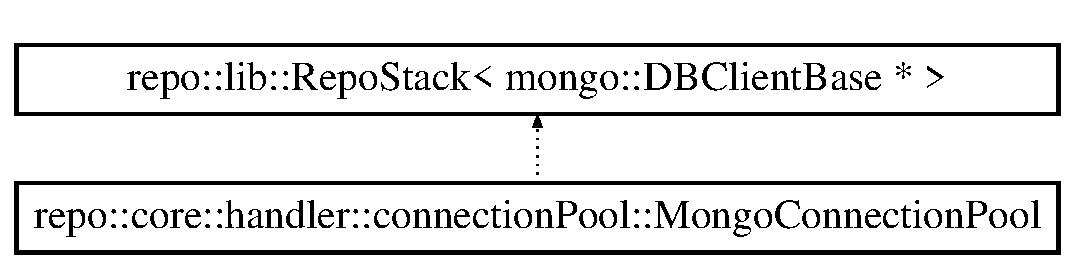
\includegraphics[height=2.000000cm]{classrepo_1_1core_1_1handler_1_1connection_pool_1_1_mongo_connection_pool}
\end{center}
\end{figure}
\subsection*{Public Member Functions}
\begin{DoxyCompactItemize}
\item 
\hyperlink{classrepo_1_1core_1_1handler_1_1connection_pool_1_1_mongo_connection_pool_a545c2e6f439318da4dfc68d7c48e1df1}{Mongo\+Connection\+Pool} (const int \&num\+Connections, mongo\+::\+Connection\+String db\+Address, mongo\+::\+B\+S\+O\+N\+Obj $\ast$auth)
\item 
\hypertarget{classrepo_1_1core_1_1handler_1_1connection_pool_1_1_mongo_connection_pool_af448f2923d7cab7c29e88065395290a6}{}mongo\+::\+D\+B\+Client\+Base $\ast$ {\bfseries get\+Worker} ()\label{classrepo_1_1core_1_1handler_1_1connection_pool_1_1_mongo_connection_pool_af448f2923d7cab7c29e88065395290a6}

\item 
\hypertarget{classrepo_1_1core_1_1handler_1_1connection_pool_1_1_mongo_connection_pool_a42c2d9342df8b7aac1ca4ceff4fa0106}{}void {\bfseries return\+Worker} (mongo\+::\+D\+B\+Client\+Base $\ast$worker)\label{classrepo_1_1core_1_1handler_1_1connection_pool_1_1_mongo_connection_pool_a42c2d9342df8b7aac1ca4ceff4fa0106}

\item 
\hypertarget{classrepo_1_1core_1_1handler_1_1connection_pool_1_1_mongo_connection_pool_a6a5f6613da30e6ba531018fc70fbfd04}{}mongo\+::\+D\+B\+Client\+Base $\ast$ {\bfseries pop} ()\label{classrepo_1_1core_1_1handler_1_1connection_pool_1_1_mongo_connection_pool_a6a5f6613da30e6ba531018fc70fbfd04}

\item 
\hypertarget{classrepo_1_1core_1_1handler_1_1connection_pool_1_1_mongo_connection_pool_ae60f4f074bee5cb799c17363c3d03c38}{}void {\bfseries push} (mongo\+::\+D\+B\+Client\+Base $\ast$worker)\label{classrepo_1_1core_1_1handler_1_1connection_pool_1_1_mongo_connection_pool_ae60f4f074bee5cb799c17363c3d03c38}

\end{DoxyCompactItemize}


\subsection{Constructor \& Destructor Documentation}
\hypertarget{classrepo_1_1core_1_1handler_1_1connection_pool_1_1_mongo_connection_pool_a545c2e6f439318da4dfc68d7c48e1df1}{}\index{repo\+::core\+::handler\+::connection\+Pool\+::\+Mongo\+Connection\+Pool@{repo\+::core\+::handler\+::connection\+Pool\+::\+Mongo\+Connection\+Pool}!Mongo\+Connection\+Pool@{Mongo\+Connection\+Pool}}
\index{Mongo\+Connection\+Pool@{Mongo\+Connection\+Pool}!repo\+::core\+::handler\+::connection\+Pool\+::\+Mongo\+Connection\+Pool@{repo\+::core\+::handler\+::connection\+Pool\+::\+Mongo\+Connection\+Pool}}
\subsubsection[{Mongo\+Connection\+Pool}]{\setlength{\rightskip}{0pt plus 5cm}repo\+::core\+::handler\+::connection\+Pool\+::\+Mongo\+Connection\+Pool\+::\+Mongo\+Connection\+Pool (
\begin{DoxyParamCaption}
\item[{const int \&}]{num\+Connections, }
\item[{mongo\+::\+Connection\+String}]{db\+Address, }
\item[{mongo\+::\+B\+S\+O\+N\+Obj $\ast$}]{auth}
\end{DoxyParamCaption}
)\hspace{0.3cm}{\ttfamily [inline]}}\label{classrepo_1_1core_1_1handler_1_1connection_pool_1_1_mongo_connection_pool_a545c2e6f439318da4dfc68d7c48e1df1}
Instantiate the pool of workers with a limited number of connections 
\begin{DoxyParams}{Parameters}
{\em num\+Connections} & number of connections \\
\hline
\end{DoxyParams}


The documentation for this class was generated from the following file\+:\begin{DoxyCompactItemize}
\item 
C\+:/\+Users/\+Carmen/3\+D Repo/\+Repo/3drepobouncer/bouncer/src/repo/core/handler/connectionpool/repo\+\_\+connection\+\_\+pool\+\_\+mongo.\+h\end{DoxyCompactItemize}

\hypertarget{classrepo_1_1core_1_1handler_1_1_mongo_database_handler}{}\section{repo\+:\+:core\+:\+:handler\+:\+:Mongo\+Database\+Handler Class Reference}
\label{classrepo_1_1core_1_1handler_1_1_mongo_database_handler}\index{repo\+::core\+::handler\+::\+Mongo\+Database\+Handler@{repo\+::core\+::handler\+::\+Mongo\+Database\+Handler}}
Inheritance diagram for repo\+:\+:core\+:\+:handler\+:\+:Mongo\+Database\+Handler\+:\begin{figure}[H]
\begin{center}
\leavevmode
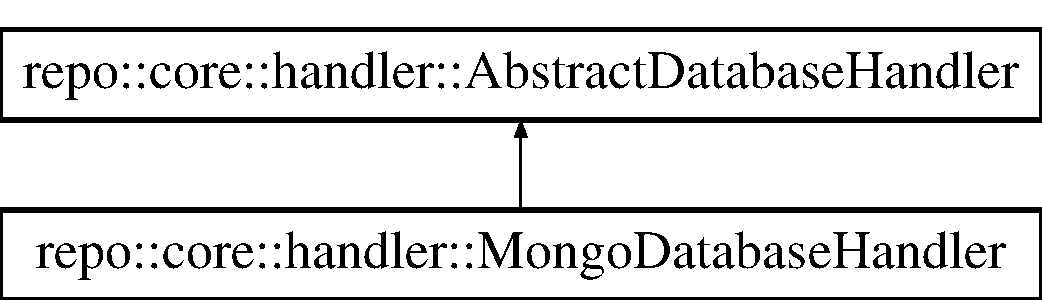
\includegraphics[height=2.000000cm]{classrepo_1_1core_1_1handler_1_1_mongo_database_handler}
\end{center}
\end{figure}
\subsection*{Public Member Functions}
\begin{DoxyCompactItemize}
\item 
\hyperlink{classrepo_1_1core_1_1handler_1_1_mongo_database_handler_a5a8444437b564686632dce0ec6f592fb}{$\sim$\+Mongo\+Database\+Handler} ()
\item 
uint64\+\_\+t \hyperlink{classrepo_1_1core_1_1handler_1_1_mongo_database_handler_ad69882e8c3573be494c5b6eca6a53827}{count\+Items\+In\+Collection} (const std\+::string \&database, const std\+::string \&collection, std\+::string \&err\+Msg)
\item 
std\+::vector$<$ \hyperlink{classrepo_1_1core_1_1model_1_1_repo_b_s_o_n}{repo\+::core\+::model\+::\+Repo\+B\+S\+O\+N} $>$ \hyperlink{classrepo_1_1core_1_1handler_1_1_mongo_database_handler_a3083dc4c2983681aa2b356c87bcaeca3}{get\+All\+From\+Collection\+Tailable} (const std\+::string \&database, const std\+::string \&collection, const uint64\+\_\+t \&skip=0, const uint32\+\_\+t \&limit=0, const std\+::list$<$ std\+::string $>$ \&fields=std\+::list$<$ std\+::string $>$(), const std\+::string \&sort\+Field=std\+::string(), const int \&sort\+Order=-\/1)
\item 
std\+::list$<$ std\+::string $>$ \hyperlink{classrepo_1_1core_1_1handler_1_1_mongo_database_handler_ad51771cf9bca612634c4e761266c5d32}{get\+Collections} (const std\+::string \&database)
\item 
\hyperlink{classrepo_1_1core_1_1model_1_1_collection_stats}{repo\+::core\+::model\+::\+Collection\+Stats} \hyperlink{classrepo_1_1core_1_1handler_1_1_mongo_database_handler_a61020c951e94df65b9afb29bcd5472d7}{get\+Collection\+Stats} (const std\+::string \&database, const std\+::string \&collection, std\+::string \&err\+Msg)
\item 
std\+::list$<$ std\+::string $>$ \hyperlink{classrepo_1_1core_1_1handler_1_1_mongo_database_handler_ad87a0ae0ba7fb783479d399b6f98ee67}{get\+Databases} (const bool \&sorted=true)
\item 
std\+::map$<$ std\+::string, std\+::list$<$ std\+::string $>$ $>$ \hyperlink{classrepo_1_1core_1_1handler_1_1_mongo_database_handler_aa6ad44a0cde0f642d52cc92a61178739}{get\+Databases\+With\+Projects} (const std\+::list$<$ std\+::string $>$ \&databases, const std\+::string \&project\+Ext=\char`\"{}history\char`\"{})
\item 
std\+::list$<$ std\+::string $>$ \hyperlink{classrepo_1_1core_1_1handler_1_1_mongo_database_handler_a84c34b3c1f0ba3227d4a159176bdfb7f}{get\+Projects} (const std\+::string \&database, const std\+::string \&project\+Ext)
\item 
std\+::list$<$ std\+::string $>$ \hyperlink{classrepo_1_1core_1_1handler_1_1_mongo_database_handler_afeaa95dcb44d7a1276fa1e90a5987f6d}{get\+Admin\+Database\+Roles} ()
\item 
std\+::list$<$ std\+::string $>$ \hyperlink{classrepo_1_1core_1_1handler_1_1_mongo_database_handler_a9974cd3f7f955793cbe56eab74ced573}{get\+Standard\+Database\+Roles} ()
\item 
virtual void \hyperlink{classrepo_1_1core_1_1handler_1_1_mongo_database_handler_abeaad0e73b0e274755e7ee2baab002ae}{create\+Collection} (const std\+::string \&database, const std\+::string \&name)
\item 
bool \hyperlink{classrepo_1_1core_1_1handler_1_1_mongo_database_handler_a7c4cdb628a1b3c59caba6b397fe20375}{drop\+Collection} (const std\+::string \&database, const std\+::string \&collection, std\+::string \&err\+Msg)
\item 
bool \hyperlink{classrepo_1_1core_1_1handler_1_1_mongo_database_handler_ac982e4d73ee5c69d333030437eebabf6}{drop\+Database} (const std\+::string \&database, std\+::string \&err\+Msg)
\item 
bool \hyperlink{classrepo_1_1core_1_1handler_1_1_mongo_database_handler_a7e1a68ada64088e53ded91c738fadcd6}{drop\+Document} (const \hyperlink{classrepo_1_1core_1_1model_1_1_repo_b_s_o_n}{repo\+::core\+::model\+::\+Repo\+B\+S\+O\+N} bson, const std\+::string \&database, const std\+::string \&collection, std\+::string \&err\+Msg)
\item 
bool \hyperlink{classrepo_1_1core_1_1handler_1_1_mongo_database_handler_a15263c0497c215798ac7398ff89bb4d3}{drop\+Documents} (const \hyperlink{classrepo_1_1core_1_1model_1_1_repo_b_s_o_n}{repo\+::core\+::model\+::\+Repo\+B\+S\+O\+N} criteria, const std\+::string \&database, const std\+::string \&collection, std\+::string \&err\+Msg)
\item 
bool \hyperlink{classrepo_1_1core_1_1handler_1_1_mongo_database_handler_a847556c14e85da5e17f8d21c70ab23d0}{drop\+Raw\+File} (const std\+::string \&database, const std\+::string \&collection, const std\+::string \&file\+Name, std\+::string \&err\+Msg)
\item 
bool \hyperlink{classrepo_1_1core_1_1handler_1_1_mongo_database_handler_ade2b069da1314566c63a48a3b61ad451}{drop\+Role} (const \hyperlink{classrepo_1_1core_1_1model_1_1_repo_role}{repo\+::core\+::model\+::\+Repo\+Role} \&role, std\+::string \&errmsg)
\item 
bool \hyperlink{classrepo_1_1core_1_1handler_1_1_mongo_database_handler_ad5e1716d61ffe74086453ae4d0bbad24}{drop\+User} (const \hyperlink{classrepo_1_1core_1_1model_1_1_repo_user}{repo\+::core\+::model\+::\+Repo\+User} \&user, std\+::string \&errmsg)
\item 
bool \hyperlink{classrepo_1_1core_1_1handler_1_1_mongo_database_handler_a8b25a7efcb68ee809fd6b6ea20cb06ae}{insert\+Document} (const std\+::string \&database, const std\+::string \&collection, const \hyperlink{classrepo_1_1core_1_1model_1_1_repo_b_s_o_n}{repo\+::core\+::model\+::\+Repo\+B\+S\+O\+N} \&obj, std\+::string \&err\+Msg)
\item 
bool \hyperlink{classrepo_1_1core_1_1handler_1_1_mongo_database_handler_abaeb1612b1beb0945c72b153932d274f}{insert\+Raw\+File} (const std\+::string \&database, const std\+::string \&collection, const std\+::string \&file\+Name, const std\+::vector$<$ uint8\+\_\+t $>$ \&bin, std\+::string \&err\+Msg, const std\+::string \&content\+Type=\char`\"{}binary/octet-\/stream\char`\"{})
\item 
bool \hyperlink{classrepo_1_1core_1_1handler_1_1_mongo_database_handler_a1366832cc771fd306b0058ba4e1dcf30}{insert\+Role} (const \hyperlink{classrepo_1_1core_1_1model_1_1_repo_role}{repo\+::core\+::model\+::\+Repo\+Role} \&role, std\+::string \&errmsg)
\item 
bool \hyperlink{classrepo_1_1core_1_1handler_1_1_mongo_database_handler_acf2b49877a7d8a914e1a1d2aeb1b60e8}{insert\+User} (const \hyperlink{classrepo_1_1core_1_1model_1_1_repo_user}{repo\+::core\+::model\+::\+Repo\+User} \&user, std\+::string \&errmsg)
\item 
bool \hyperlink{classrepo_1_1core_1_1handler_1_1_mongo_database_handler_a81743d1af17889ad66a76b7ede0f420e}{upsert\+Document} (const std\+::string \&database, const std\+::string \&collection, const \hyperlink{classrepo_1_1core_1_1model_1_1_repo_b_s_o_n}{repo\+::core\+::model\+::\+Repo\+B\+S\+O\+N} \&obj, const bool \&overwrite, std\+::string \&err\+Msg)
\item 
bool \hyperlink{classrepo_1_1core_1_1handler_1_1_mongo_database_handler_a14c38b79dedf9e26bf802771367ebace}{update\+Role} (const \hyperlink{classrepo_1_1core_1_1model_1_1_repo_role}{repo\+::core\+::model\+::\+Repo\+Role} \&role, std\+::string \&errmsg)
\item 
bool \hyperlink{classrepo_1_1core_1_1handler_1_1_mongo_database_handler_a7fae7458d4261fc61a7415262813183d}{update\+User} (const \hyperlink{classrepo_1_1core_1_1model_1_1_repo_user}{repo\+::core\+::model\+::\+Repo\+User} \&user, std\+::string \&errmsg)
\item 
std\+::vector$<$ \hyperlink{classrepo_1_1core_1_1model_1_1_repo_b_s_o_n}{repo\+::core\+::model\+::\+Repo\+B\+S\+O\+N} $>$ \hyperlink{classrepo_1_1core_1_1handler_1_1_mongo_database_handler_a26cca6e23ce8e218fe5c6106bc91425a}{find\+All\+By\+Unique\+I\+Ds} (const std\+::string \&database, const std\+::string \&collection, const \hyperlink{classrepo_1_1core_1_1model_1_1_repo_b_s_o_n}{repo\+::core\+::model\+::\+Repo\+B\+S\+O\+N} \&uuids)
\item 
std\+::vector$<$ \hyperlink{classrepo_1_1core_1_1model_1_1_repo_b_s_o_n}{repo\+::core\+::model\+::\+Repo\+B\+S\+O\+N} $>$ \hyperlink{classrepo_1_1core_1_1handler_1_1_mongo_database_handler_af8bc6c5531e6669b9ac278c6fc64ec3e}{find\+All\+By\+Criteria} (const std\+::string \&database, const std\+::string \&collection, const \hyperlink{classrepo_1_1core_1_1model_1_1_repo_b_s_o_n}{repo\+::core\+::model\+::\+Repo\+B\+S\+O\+N} \&criteria)
\item 
\hyperlink{classrepo_1_1core_1_1model_1_1_repo_b_s_o_n}{repo\+::core\+::model\+::\+Repo\+B\+S\+O\+N} \hyperlink{classrepo_1_1core_1_1handler_1_1_mongo_database_handler_a9e13fe73ff838e388378d82673964e20}{find\+One\+By\+Criteria} (const std\+::string \&database, const std\+::string \&collection, const \hyperlink{classrepo_1_1core_1_1model_1_1_repo_b_s_o_n}{repo\+::core\+::model\+::\+Repo\+B\+S\+O\+N} \&criteria, const std\+::string \&sort\+Field=\char`\"{}\char`\"{})
\item 
\hyperlink{classrepo_1_1core_1_1model_1_1_repo_b_s_o_n}{repo\+::core\+::model\+::\+Repo\+B\+S\+O\+N} \hyperlink{classrepo_1_1core_1_1handler_1_1_mongo_database_handler_aae7c0539fcdbad26c307c9f63877d536}{find\+One\+By\+Shared\+I\+D} (const std\+::string \&database, const std\+::string \&collection, const repo\+U\+U\+I\+D \&uuid, const std\+::string \&sort\+Field)
\item 
\hyperlink{classrepo_1_1core_1_1model_1_1_repo_b_s_o_n}{repo\+::core\+::model\+::\+Repo\+B\+S\+O\+N} \hyperlink{classrepo_1_1core_1_1handler_1_1_mongo_database_handler_ac016547468fc0049c859d775e270e17a}{find\+One\+By\+Unique\+I\+D} (const std\+::string \&database, const std\+::string \&collection, const repo\+U\+U\+I\+D \&uuid)
\item 
std\+::vector$<$ uint8\+\_\+t $>$ \hyperlink{classrepo_1_1core_1_1handler_1_1_mongo_database_handler_abcdf4cc7cbc0bbee8b9236349bde8364}{get\+Raw\+File} (const std\+::string \&database, const std\+::string \&collection, const std\+::string \&fname)
\end{DoxyCompactItemize}
\subsection*{Static Public Member Functions}
\begin{DoxyCompactItemize}
\item 
static void \hyperlink{classrepo_1_1core_1_1handler_1_1_mongo_database_handler_adad19607d035f2cd335f8fa2b7afa94f}{disconnect\+Handler} ()
\item 
static \hyperlink{classrepo_1_1core_1_1handler_1_1_mongo_database_handler}{Mongo\+Database\+Handler} $\ast$ \hyperlink{classrepo_1_1core_1_1handler_1_1_mongo_database_handler_a3efffd91168321728dcb28fc80eabd0a}{get\+Handler} (std\+::string \&err\+Msg, const std\+::string \&host, const int \&port, const uint32\+\_\+t \&max\+Connections=1, const std\+::string \&db\+Name=std\+::string(), const std\+::string \&username=std\+::string(), const std\+::string \&password=std\+::string(), const bool \&pw\+Digested=false)
\item 
static \hyperlink{classrepo_1_1core_1_1handler_1_1_mongo_database_handler}{Mongo\+Database\+Handler} $\ast$ \hyperlink{classrepo_1_1core_1_1handler_1_1_mongo_database_handler_a0432cb604d05dba64424f71bf4df6d39}{get\+Handler} (std\+::string \&err\+Msg, const std\+::string \&host, const int \&port, const uint32\+\_\+t \&max\+Connections, const std\+::string \&db\+Name=std\+::string(), const \hyperlink{classrepo_1_1core_1_1model_1_1_repo_b_s_o_n}{model\+::\+Repo\+B\+S\+O\+N} $\ast$credentials=nullptr)
\item 
static \hyperlink{classrepo_1_1core_1_1handler_1_1_mongo_database_handler}{Mongo\+Database\+Handler} $\ast$ \hyperlink{classrepo_1_1core_1_1handler_1_1_mongo_database_handler_ac7eda2da76c1fbe02bf523e207cf9d4d}{get\+Handler} (const std\+::string \&host)
\item 
static \hyperlink{classrepo_1_1core_1_1model_1_1_repo_b_s_o_n}{repo\+::core\+::model\+::\+Repo\+B\+S\+O\+N} $\ast$ \hyperlink{classrepo_1_1core_1_1handler_1_1_mongo_database_handler_a5605412c0f2586385dec3d279ba7591d}{create\+B\+S\+O\+N\+Credentials} (const std\+::string \&db\+Name, const std\+::string \&username, const std\+::string \&password, const bool \&pw\+Digested=false)
\item 
static std\+::string \hyperlink{classrepo_1_1core_1_1handler_1_1_mongo_database_handler_ae0e35b94deb711a346459ec88a57199c}{get\+Admin\+Database\+Name} ()
\end{DoxyCompactItemize}
\subsection*{Static Public Attributes}
\begin{DoxyCompactItemize}
\item 
\hypertarget{classrepo_1_1core_1_1handler_1_1_mongo_database_handler_ab55d3d2e445e6b56b8b2aeaefcf41c07}{}static const std\+::string {\bfseries I\+D} = \char`\"{}\+\_\+id\char`\"{}\label{classrepo_1_1core_1_1handler_1_1_mongo_database_handler_ab55d3d2e445e6b56b8b2aeaefcf41c07}

\item 
\hypertarget{classrepo_1_1core_1_1handler_1_1_mongo_database_handler_a75e5efc0b9ec2e40fa23bf46fd7af53b}{}static const std\+::string \hyperlink{classrepo_1_1core_1_1handler_1_1_mongo_database_handler_a75e5efc0b9ec2e40fa23bf46fd7af53b}{U\+U\+I\+D} = \char`\"{}uuid\char`\"{}\label{classrepo_1_1core_1_1handler_1_1_mongo_database_handler_a75e5efc0b9ec2e40fa23bf46fd7af53b}

\begin{DoxyCompactList}\small\item\em \char`\"{}\+\_\+id\char`\"{} \end{DoxyCompactList}\item 
\hypertarget{classrepo_1_1core_1_1handler_1_1_mongo_database_handler_a62321508d0b278c72036d7be7b138f9c}{}static const std\+::string \hyperlink{classrepo_1_1core_1_1handler_1_1_mongo_database_handler_a62321508d0b278c72036d7be7b138f9c}{A\+D\+M\+I\+N\+\_\+\+D\+A\+T\+A\+B\+A\+S\+E} = \char`\"{}admin\char`\"{}\label{classrepo_1_1core_1_1handler_1_1_mongo_database_handler_a62321508d0b278c72036d7be7b138f9c}

\begin{DoxyCompactList}\small\item\em \char`\"{}uuid\char`\"{} \end{DoxyCompactList}\item 
\hypertarget{classrepo_1_1core_1_1handler_1_1_mongo_database_handler_ada63d3d522b76c50732b17a461224c9a}{}static const std\+::string \hyperlink{classrepo_1_1core_1_1handler_1_1_mongo_database_handler_ada63d3d522b76c50732b17a461224c9a}{S\+Y\+S\+T\+E\+M\+\_\+\+R\+O\+L\+E\+S\+\_\+\+C\+O\+L\+L\+E\+C\+T\+I\+O\+N} = \char`\"{}system.\+roles\char`\"{}\label{classrepo_1_1core_1_1handler_1_1_mongo_database_handler_ada63d3d522b76c50732b17a461224c9a}

\begin{DoxyCompactList}\small\item\em \char`\"{}admin\char`\"{} \end{DoxyCompactList}\item 
\hypertarget{classrepo_1_1core_1_1handler_1_1_mongo_database_handler_a6a6c5aac7181c5190920fc7b4f250b97}{}static const std\+::string \hyperlink{classrepo_1_1core_1_1handler_1_1_mongo_database_handler_a6a6c5aac7181c5190920fc7b4f250b97}{A\+U\+T\+H\+\_\+\+M\+E\+C\+H}\label{classrepo_1_1core_1_1handler_1_1_mongo_database_handler_a6a6c5aac7181c5190920fc7b4f250b97}

\begin{DoxyCompactList}\small\item\em \char`\"{}system.\+roles\char`\"{} \end{DoxyCompactList}\item 
static const std\+::list$<$ std\+::string $>$ \hyperlink{classrepo_1_1core_1_1handler_1_1_mongo_database_handler_a963d231d4bb42ae5ac36f70eddbb8068}{A\+N\+Y\+\_\+\+D\+A\+T\+A\+B\+A\+S\+E\+\_\+\+R\+O\+L\+E\+S}
\begin{DoxyCompactList}\small\item\em Built in any database roles. See \href{http://docs.mongodb.org/manual/reference/built-in-roles/}{\tt http\+://docs.\+mongodb.\+org/manual/reference/built-\/in-\/roles/}. \end{DoxyCompactList}\item 
static const std\+::list$<$ std\+::string $>$ \hyperlink{classrepo_1_1core_1_1handler_1_1_mongo_database_handler_aef93abfc2e7cdf3108aa8cc170c2cc69}{A\+D\+M\+I\+N\+\_\+\+O\+N\+L\+Y\+\_\+\+D\+A\+T\+A\+B\+A\+S\+E\+\_\+\+R\+O\+L\+E\+S}
\begin{DoxyCompactList}\small\item\em Built in admin database roles. See \href{http://docs.mongodb.org/manual/reference/built-in-roles/}{\tt http\+://docs.\+mongodb.\+org/manual/reference/built-\/in-\/roles/}. \end{DoxyCompactList}\end{DoxyCompactItemize}
\subsection*{Static Protected Attributes}
\begin{DoxyCompactItemize}
\item 
\hypertarget{classrepo_1_1core_1_1handler_1_1_mongo_database_handler_a98e94b48236aea664f31f22698885396}{}static \hyperlink{classrepo_1_1core_1_1handler_1_1_mongo_database_handler}{Mongo\+Database\+Handler} $\ast$ {\bfseries handler} = N\+U\+L\+L\label{classrepo_1_1core_1_1handler_1_1_mongo_database_handler_a98e94b48236aea664f31f22698885396}

\end{DoxyCompactItemize}
\subsection*{Additional Inherited Members}


\subsection{Constructor \& Destructor Documentation}
\hypertarget{classrepo_1_1core_1_1handler_1_1_mongo_database_handler_a5a8444437b564686632dce0ec6f592fb}{}\index{repo\+::core\+::handler\+::\+Mongo\+Database\+Handler@{repo\+::core\+::handler\+::\+Mongo\+Database\+Handler}!````~Mongo\+Database\+Handler@{$\sim$\+Mongo\+Database\+Handler}}
\index{````~Mongo\+Database\+Handler@{$\sim$\+Mongo\+Database\+Handler}!repo\+::core\+::handler\+::\+Mongo\+Database\+Handler@{repo\+::core\+::handler\+::\+Mongo\+Database\+Handler}}
\subsubsection[{$\sim$\+Mongo\+Database\+Handler}]{\setlength{\rightskip}{0pt plus 5cm}Mongo\+Database\+Handler\+::$\sim$\+Mongo\+Database\+Handler (
\begin{DoxyParamCaption}
{}
\end{DoxyParamCaption}
)}\label{classrepo_1_1core_1_1handler_1_1_mongo_database_handler_a5a8444437b564686632dce0ec6f592fb}
A Deconstructor 

\subsection{Member Function Documentation}
\hypertarget{classrepo_1_1core_1_1handler_1_1_mongo_database_handler_ad69882e8c3573be494c5b6eca6a53827}{}\index{repo\+::core\+::handler\+::\+Mongo\+Database\+Handler@{repo\+::core\+::handler\+::\+Mongo\+Database\+Handler}!count\+Items\+In\+Collection@{count\+Items\+In\+Collection}}
\index{count\+Items\+In\+Collection@{count\+Items\+In\+Collection}!repo\+::core\+::handler\+::\+Mongo\+Database\+Handler@{repo\+::core\+::handler\+::\+Mongo\+Database\+Handler}}
\subsubsection[{count\+Items\+In\+Collection}]{\setlength{\rightskip}{0pt plus 5cm}uint64\+\_\+t Mongo\+Database\+Handler\+::count\+Items\+In\+Collection (
\begin{DoxyParamCaption}
\item[{const std\+::string \&}]{database, }
\item[{const std\+::string \&}]{collection, }
\item[{std\+::string \&}]{err\+Msg}
\end{DoxyParamCaption}
)\hspace{0.3cm}{\ttfamily [virtual]}}\label{classrepo_1_1core_1_1handler_1_1_mongo_database_handler_ad69882e8c3573be494c5b6eca6a53827}
Count the number of documents within the collection 
\begin{DoxyParams}{Parameters}
{\em database} & name of database \\
\hline
{\em collection} & name of collection \\
\hline
{\em err\+Msg} & err\+Msg if failed \\
\hline
\end{DoxyParams}
\begin{DoxyReturn}{Returns}
number of documents within the specified collection 
\end{DoxyReturn}


Implements \hyperlink{classrepo_1_1core_1_1handler_1_1_abstract_database_handler_a862cb79b547fbd5a524a2f75ae114907}{repo\+::core\+::handler\+::\+Abstract\+Database\+Handler}.

\hypertarget{classrepo_1_1core_1_1handler_1_1_mongo_database_handler_a5605412c0f2586385dec3d279ba7591d}{}\index{repo\+::core\+::handler\+::\+Mongo\+Database\+Handler@{repo\+::core\+::handler\+::\+Mongo\+Database\+Handler}!create\+B\+S\+O\+N\+Credentials@{create\+B\+S\+O\+N\+Credentials}}
\index{create\+B\+S\+O\+N\+Credentials@{create\+B\+S\+O\+N\+Credentials}!repo\+::core\+::handler\+::\+Mongo\+Database\+Handler@{repo\+::core\+::handler\+::\+Mongo\+Database\+Handler}}
\subsubsection[{create\+B\+S\+O\+N\+Credentials}]{\setlength{\rightskip}{0pt plus 5cm}static {\bf repo\+::core\+::model\+::\+Repo\+B\+S\+O\+N}$\ast$ repo\+::core\+::handler\+::\+Mongo\+Database\+Handler\+::create\+B\+S\+O\+N\+Credentials (
\begin{DoxyParamCaption}
\item[{const std\+::string \&}]{db\+Name, }
\item[{const std\+::string \&}]{username, }
\item[{const std\+::string \&}]{password, }
\item[{const bool \&}]{pw\+Digested = {\ttfamily false}}
\end{DoxyParamCaption}
)\hspace{0.3cm}{\ttfamily [inline]}, {\ttfamily [static]}}\label{classrepo_1_1core_1_1handler_1_1_mongo_database_handler_a5605412c0f2586385dec3d279ba7591d}
Generates a B\+S\+O\+N object containing user credentials 
\begin{DoxyParams}{Parameters}
{\em db\+Name} & name of the database to authenticate against \\
\hline
{\em username} & user name for authentication \\
\hline
{\em password} & password of the user \\
\hline
{\em pw\+Digested} & true if pw is digested \\
\hline
\end{DoxyParams}
\begin{DoxyReturn}{Returns}
returns the constructed B\+S\+O\+N object, or 0 nullptr username is empty 
\end{DoxyReturn}
\hypertarget{classrepo_1_1core_1_1handler_1_1_mongo_database_handler_abeaad0e73b0e274755e7ee2baab002ae}{}\index{repo\+::core\+::handler\+::\+Mongo\+Database\+Handler@{repo\+::core\+::handler\+::\+Mongo\+Database\+Handler}!create\+Collection@{create\+Collection}}
\index{create\+Collection@{create\+Collection}!repo\+::core\+::handler\+::\+Mongo\+Database\+Handler@{repo\+::core\+::handler\+::\+Mongo\+Database\+Handler}}
\subsubsection[{create\+Collection}]{\setlength{\rightskip}{0pt plus 5cm}void Mongo\+Database\+Handler\+::create\+Collection (
\begin{DoxyParamCaption}
\item[{const std\+::string \&}]{database, }
\item[{const std\+::string \&}]{name}
\end{DoxyParamCaption}
)\hspace{0.3cm}{\ttfamily [virtual]}}\label{classrepo_1_1core_1_1handler_1_1_mongo_database_handler_abeaad0e73b0e274755e7ee2baab002ae}
Create a collection with the name specified 
\begin{DoxyParams}{Parameters}
{\em database} & name of the database \\
\hline
{\em name} & name of the collection \\
\hline
\end{DoxyParams}


Implements \hyperlink{classrepo_1_1core_1_1handler_1_1_abstract_database_handler_a55a28fe47b164cb4578cb4e682759439}{repo\+::core\+::handler\+::\+Abstract\+Database\+Handler}.

\hypertarget{classrepo_1_1core_1_1handler_1_1_mongo_database_handler_adad19607d035f2cd335f8fa2b7afa94f}{}\index{repo\+::core\+::handler\+::\+Mongo\+Database\+Handler@{repo\+::core\+::handler\+::\+Mongo\+Database\+Handler}!disconnect\+Handler@{disconnect\+Handler}}
\index{disconnect\+Handler@{disconnect\+Handler}!repo\+::core\+::handler\+::\+Mongo\+Database\+Handler@{repo\+::core\+::handler\+::\+Mongo\+Database\+Handler}}
\subsubsection[{disconnect\+Handler}]{\setlength{\rightskip}{0pt plus 5cm}void Mongo\+Database\+Handler\+::disconnect\+Handler (
\begin{DoxyParamCaption}
{}
\end{DoxyParamCaption}
)\hspace{0.3cm}{\ttfamily [static]}}\label{classrepo_1_1core_1_1handler_1_1_mongo_database_handler_adad19607d035f2cd335f8fa2b7afa94f}
Disconnects the handler and resets the instance Must call this before trying to reconnect to another database! \hypertarget{classrepo_1_1core_1_1handler_1_1_mongo_database_handler_a7c4cdb628a1b3c59caba6b397fe20375}{}\index{repo\+::core\+::handler\+::\+Mongo\+Database\+Handler@{repo\+::core\+::handler\+::\+Mongo\+Database\+Handler}!drop\+Collection@{drop\+Collection}}
\index{drop\+Collection@{drop\+Collection}!repo\+::core\+::handler\+::\+Mongo\+Database\+Handler@{repo\+::core\+::handler\+::\+Mongo\+Database\+Handler}}
\subsubsection[{drop\+Collection}]{\setlength{\rightskip}{0pt plus 5cm}bool Mongo\+Database\+Handler\+::drop\+Collection (
\begin{DoxyParamCaption}
\item[{const std\+::string \&}]{database, }
\item[{const std\+::string \&}]{collection, }
\item[{std\+::string \&}]{err\+Msg}
\end{DoxyParamCaption}
)\hspace{0.3cm}{\ttfamily [virtual]}}\label{classrepo_1_1core_1_1handler_1_1_mongo_database_handler_a7c4cdb628a1b3c59caba6b397fe20375}
Remove a collection from the database 
\begin{DoxyParams}{Parameters}
{\em database} & the database the collection resides in \\
\hline
{\em collection} & name of the collection to drop \\
\hline
{\em err\+Msg} & name of the collection to drop \\
\hline
\end{DoxyParams}


Implements \hyperlink{classrepo_1_1core_1_1handler_1_1_abstract_database_handler_ab268b2a7d4e0ae0499d016d3311767e7}{repo\+::core\+::handler\+::\+Abstract\+Database\+Handler}.

\hypertarget{classrepo_1_1core_1_1handler_1_1_mongo_database_handler_ac982e4d73ee5c69d333030437eebabf6}{}\index{repo\+::core\+::handler\+::\+Mongo\+Database\+Handler@{repo\+::core\+::handler\+::\+Mongo\+Database\+Handler}!drop\+Database@{drop\+Database}}
\index{drop\+Database@{drop\+Database}!repo\+::core\+::handler\+::\+Mongo\+Database\+Handler@{repo\+::core\+::handler\+::\+Mongo\+Database\+Handler}}
\subsubsection[{drop\+Database}]{\setlength{\rightskip}{0pt plus 5cm}bool Mongo\+Database\+Handler\+::drop\+Database (
\begin{DoxyParamCaption}
\item[{const std\+::string \&}]{database, }
\item[{std\+::string \&}]{err\+Msg}
\end{DoxyParamCaption}
)\hspace{0.3cm}{\ttfamily [virtual]}}\label{classrepo_1_1core_1_1handler_1_1_mongo_database_handler_ac982e4d73ee5c69d333030437eebabf6}
Remove a database from the mongo database 
\begin{DoxyParams}{Parameters}
{\em database} & name of the database to drop \\
\hline
{\em err\+Msg} & name of the database to drop \\
\hline
\end{DoxyParams}


Implements \hyperlink{classrepo_1_1core_1_1handler_1_1_abstract_database_handler_ad169812ef62d6d21a02d5545633492c0}{repo\+::core\+::handler\+::\+Abstract\+Database\+Handler}.

\hypertarget{classrepo_1_1core_1_1handler_1_1_mongo_database_handler_a7e1a68ada64088e53ded91c738fadcd6}{}\index{repo\+::core\+::handler\+::\+Mongo\+Database\+Handler@{repo\+::core\+::handler\+::\+Mongo\+Database\+Handler}!drop\+Document@{drop\+Document}}
\index{drop\+Document@{drop\+Document}!repo\+::core\+::handler\+::\+Mongo\+Database\+Handler@{repo\+::core\+::handler\+::\+Mongo\+Database\+Handler}}
\subsubsection[{drop\+Document}]{\setlength{\rightskip}{0pt plus 5cm}bool Mongo\+Database\+Handler\+::drop\+Document (
\begin{DoxyParamCaption}
\item[{const {\bf repo\+::core\+::model\+::\+Repo\+B\+S\+O\+N}}]{bson, }
\item[{const std\+::string \&}]{database, }
\item[{const std\+::string \&}]{collection, }
\item[{std\+::string \&}]{err\+Msg}
\end{DoxyParamCaption}
)\hspace{0.3cm}{\ttfamily [virtual]}}\label{classrepo_1_1core_1_1handler_1_1_mongo_database_handler_a7e1a68ada64088e53ded91c738fadcd6}
Remove a document from the mongo database 
\begin{DoxyParams}{Parameters}
{\em bson} & document to remove \\
\hline
{\em database} & the database the collection resides in \\
\hline
{\em collection} & name of the collection the document is in \\
\hline
{\em err\+Msg} & name of the database to drop \\
\hline
\end{DoxyParams}


Implements \hyperlink{classrepo_1_1core_1_1handler_1_1_abstract_database_handler_a189685c88cbadb3f239829d65d4dcb3b}{repo\+::core\+::handler\+::\+Abstract\+Database\+Handler}.

\hypertarget{classrepo_1_1core_1_1handler_1_1_mongo_database_handler_a15263c0497c215798ac7398ff89bb4d3}{}\index{repo\+::core\+::handler\+::\+Mongo\+Database\+Handler@{repo\+::core\+::handler\+::\+Mongo\+Database\+Handler}!drop\+Documents@{drop\+Documents}}
\index{drop\+Documents@{drop\+Documents}!repo\+::core\+::handler\+::\+Mongo\+Database\+Handler@{repo\+::core\+::handler\+::\+Mongo\+Database\+Handler}}
\subsubsection[{drop\+Documents}]{\setlength{\rightskip}{0pt plus 5cm}bool Mongo\+Database\+Handler\+::drop\+Documents (
\begin{DoxyParamCaption}
\item[{const {\bf repo\+::core\+::model\+::\+Repo\+B\+S\+O\+N}}]{criteria, }
\item[{const std\+::string \&}]{database, }
\item[{const std\+::string \&}]{collection, }
\item[{std\+::string \&}]{err\+Msg}
\end{DoxyParamCaption}
)\hspace{0.3cm}{\ttfamily [virtual]}}\label{classrepo_1_1core_1_1handler_1_1_mongo_database_handler_a15263c0497c215798ac7398ff89bb4d3}
Remove all documents satisfying a certain criteria 
\begin{DoxyParams}{Parameters}
{\em criteria} & document to remove \\
\hline
{\em database} & the database the collection resides in \\
\hline
{\em collection} & name of the collection the document is in \\
\hline
{\em err\+Msg} & name of the database to drop \\
\hline
\end{DoxyParams}


Implements \hyperlink{classrepo_1_1core_1_1handler_1_1_abstract_database_handler_a8b8cdc64a009b872ece09a4f91cdad0c}{repo\+::core\+::handler\+::\+Abstract\+Database\+Handler}.

\hypertarget{classrepo_1_1core_1_1handler_1_1_mongo_database_handler_a847556c14e85da5e17f8d21c70ab23d0}{}\index{repo\+::core\+::handler\+::\+Mongo\+Database\+Handler@{repo\+::core\+::handler\+::\+Mongo\+Database\+Handler}!drop\+Raw\+File@{drop\+Raw\+File}}
\index{drop\+Raw\+File@{drop\+Raw\+File}!repo\+::core\+::handler\+::\+Mongo\+Database\+Handler@{repo\+::core\+::handler\+::\+Mongo\+Database\+Handler}}
\subsubsection[{drop\+Raw\+File}]{\setlength{\rightskip}{0pt plus 5cm}bool Mongo\+Database\+Handler\+::drop\+Raw\+File (
\begin{DoxyParamCaption}
\item[{const std\+::string \&}]{database, }
\item[{const std\+::string \&}]{collection, }
\item[{const std\+::string \&}]{file\+Name, }
\item[{std\+::string \&}]{err\+Msg}
\end{DoxyParamCaption}
)\hspace{0.3cm}{\ttfamily [virtual]}}\label{classrepo_1_1core_1_1handler_1_1_mongo_database_handler_a847556c14e85da5e17f8d21c70ab23d0}
Remove a file from raw file storage (grid\+F\+S) 
\begin{DoxyParams}{Parameters}
{\em database} & the database the collection resides in \\
\hline
{\em collection} & name of the collection the document is in \\
\hline
{\em filename} & name of the file \\
\hline
{\em err\+Msg} & name of the database to drop \\
\hline
\end{DoxyParams}


Implements \hyperlink{classrepo_1_1core_1_1handler_1_1_abstract_database_handler_a4806eb978154c4b4bab85eb99d457318}{repo\+::core\+::handler\+::\+Abstract\+Database\+Handler}.

\hypertarget{classrepo_1_1core_1_1handler_1_1_mongo_database_handler_ade2b069da1314566c63a48a3b61ad451}{}\index{repo\+::core\+::handler\+::\+Mongo\+Database\+Handler@{repo\+::core\+::handler\+::\+Mongo\+Database\+Handler}!drop\+Role@{drop\+Role}}
\index{drop\+Role@{drop\+Role}!repo\+::core\+::handler\+::\+Mongo\+Database\+Handler@{repo\+::core\+::handler\+::\+Mongo\+Database\+Handler}}
\subsubsection[{drop\+Role}]{\setlength{\rightskip}{0pt plus 5cm}bool repo\+::core\+::handler\+::\+Mongo\+Database\+Handler\+::drop\+Role (
\begin{DoxyParamCaption}
\item[{const {\bf repo\+::core\+::model\+::\+Repo\+Role} \&}]{role, }
\item[{std\+::string \&}]{errmsg}
\end{DoxyParamCaption}
)\hspace{0.3cm}{\ttfamily [inline]}, {\ttfamily [virtual]}}\label{classrepo_1_1core_1_1handler_1_1_mongo_database_handler_ade2b069da1314566c63a48a3b61ad451}
Remove a role from the database 
\begin{DoxyParams}{Parameters}
{\em role} & user bson to remove \\
\hline
{\em errmsg} & error message \\
\hline
\end{DoxyParams}
\begin{DoxyReturn}{Returns}
returns true upon success 
\end{DoxyReturn}


Implements \hyperlink{classrepo_1_1core_1_1handler_1_1_abstract_database_handler_a65822a2183bec303c08008fadb1d17d2}{repo\+::core\+::handler\+::\+Abstract\+Database\+Handler}.

\hypertarget{classrepo_1_1core_1_1handler_1_1_mongo_database_handler_ad5e1716d61ffe74086453ae4d0bbad24}{}\index{repo\+::core\+::handler\+::\+Mongo\+Database\+Handler@{repo\+::core\+::handler\+::\+Mongo\+Database\+Handler}!drop\+User@{drop\+User}}
\index{drop\+User@{drop\+User}!repo\+::core\+::handler\+::\+Mongo\+Database\+Handler@{repo\+::core\+::handler\+::\+Mongo\+Database\+Handler}}
\subsubsection[{drop\+User}]{\setlength{\rightskip}{0pt plus 5cm}bool repo\+::core\+::handler\+::\+Mongo\+Database\+Handler\+::drop\+User (
\begin{DoxyParamCaption}
\item[{const {\bf repo\+::core\+::model\+::\+Repo\+User} \&}]{user, }
\item[{std\+::string \&}]{errmsg}
\end{DoxyParamCaption}
)\hspace{0.3cm}{\ttfamily [inline]}, {\ttfamily [virtual]}}\label{classrepo_1_1core_1_1handler_1_1_mongo_database_handler_ad5e1716d61ffe74086453ae4d0bbad24}
Remove a user from the database 
\begin{DoxyParams}{Parameters}
{\em user} & user bson to remove \\
\hline
{\em errmsg} & error message \\
\hline
\end{DoxyParams}
\begin{DoxyReturn}{Returns}
returns true upon success 
\end{DoxyReturn}


Implements \hyperlink{classrepo_1_1core_1_1handler_1_1_abstract_database_handler_a07bd15002e4c23c138a39d3b47af3882}{repo\+::core\+::handler\+::\+Abstract\+Database\+Handler}.

\hypertarget{classrepo_1_1core_1_1handler_1_1_mongo_database_handler_af8bc6c5531e6669b9ac278c6fc64ec3e}{}\index{repo\+::core\+::handler\+::\+Mongo\+Database\+Handler@{repo\+::core\+::handler\+::\+Mongo\+Database\+Handler}!find\+All\+By\+Criteria@{find\+All\+By\+Criteria}}
\index{find\+All\+By\+Criteria@{find\+All\+By\+Criteria}!repo\+::core\+::handler\+::\+Mongo\+Database\+Handler@{repo\+::core\+::handler\+::\+Mongo\+Database\+Handler}}
\subsubsection[{find\+All\+By\+Criteria}]{\setlength{\rightskip}{0pt plus 5cm}std\+::vector$<$ {\bf repo\+::core\+::model\+::\+Repo\+B\+S\+O\+N} $>$ Mongo\+Database\+Handler\+::find\+All\+By\+Criteria (
\begin{DoxyParamCaption}
\item[{const std\+::string \&}]{database, }
\item[{const std\+::string \&}]{collection, }
\item[{const {\bf repo\+::core\+::model\+::\+Repo\+B\+S\+O\+N} \&}]{criteria}
\end{DoxyParamCaption}
)\hspace{0.3cm}{\ttfamily [virtual]}}\label{classrepo_1_1core_1_1handler_1_1_mongo_database_handler_af8bc6c5531e6669b9ac278c6fc64ec3e}
Given a search criteria, find all the documents that passes this query 
\begin{DoxyParams}{Parameters}
{\em database} & name of database \\
\hline
{\em collection} & name of collection \\
\hline
{\em criteria} & search criteria in a bson object \\
\hline
\end{DoxyParams}
\begin{DoxyReturn}{Returns}
a vector of Repo\+B\+S\+O\+N objects satisfy the given criteria 
\end{DoxyReturn}


Implements \hyperlink{classrepo_1_1core_1_1handler_1_1_abstract_database_handler_ad964d9c80fcddf1444edcf7021c81e50}{repo\+::core\+::handler\+::\+Abstract\+Database\+Handler}.

\hypertarget{classrepo_1_1core_1_1handler_1_1_mongo_database_handler_a26cca6e23ce8e218fe5c6106bc91425a}{}\index{repo\+::core\+::handler\+::\+Mongo\+Database\+Handler@{repo\+::core\+::handler\+::\+Mongo\+Database\+Handler}!find\+All\+By\+Unique\+I\+Ds@{find\+All\+By\+Unique\+I\+Ds}}
\index{find\+All\+By\+Unique\+I\+Ds@{find\+All\+By\+Unique\+I\+Ds}!repo\+::core\+::handler\+::\+Mongo\+Database\+Handler@{repo\+::core\+::handler\+::\+Mongo\+Database\+Handler}}
\subsubsection[{find\+All\+By\+Unique\+I\+Ds}]{\setlength{\rightskip}{0pt plus 5cm}std\+::vector$<$ {\bf repo\+::core\+::model\+::\+Repo\+B\+S\+O\+N} $>$ Mongo\+Database\+Handler\+::find\+All\+By\+Unique\+I\+Ds (
\begin{DoxyParamCaption}
\item[{const std\+::string \&}]{database, }
\item[{const std\+::string \&}]{collection, }
\item[{const {\bf repo\+::core\+::model\+::\+Repo\+B\+S\+O\+N} \&}]{uuids}
\end{DoxyParamCaption}
)\hspace{0.3cm}{\ttfamily [virtual]}}\label{classrepo_1_1core_1_1handler_1_1_mongo_database_handler_a26cca6e23ce8e218fe5c6106bc91425a}
Given a list of unique I\+Ds, find all the documents associated to them 
\begin{DoxyParams}{Parameters}
{\em name} & of database \\
\hline
{\em name} & of collection \\
\hline
{\em array} & of uuids in a B\+S\+O\+N object \\
\hline
\end{DoxyParams}
\begin{DoxyReturn}{Returns}
a vector of Repo\+B\+S\+O\+N objects associated with the U\+U\+I\+Ds given 
\end{DoxyReturn}


Implements \hyperlink{classrepo_1_1core_1_1handler_1_1_abstract_database_handler_ad62823283064682c08acd1bd6f1414f8}{repo\+::core\+::handler\+::\+Abstract\+Database\+Handler}.

\hypertarget{classrepo_1_1core_1_1handler_1_1_mongo_database_handler_a9e13fe73ff838e388378d82673964e20}{}\index{repo\+::core\+::handler\+::\+Mongo\+Database\+Handler@{repo\+::core\+::handler\+::\+Mongo\+Database\+Handler}!find\+One\+By\+Criteria@{find\+One\+By\+Criteria}}
\index{find\+One\+By\+Criteria@{find\+One\+By\+Criteria}!repo\+::core\+::handler\+::\+Mongo\+Database\+Handler@{repo\+::core\+::handler\+::\+Mongo\+Database\+Handler}}
\subsubsection[{find\+One\+By\+Criteria}]{\setlength{\rightskip}{0pt plus 5cm}{\bf repo\+::core\+::model\+::\+Repo\+B\+S\+O\+N} Mongo\+Database\+Handler\+::find\+One\+By\+Criteria (
\begin{DoxyParamCaption}
\item[{const std\+::string \&}]{database, }
\item[{const std\+::string \&}]{collection, }
\item[{const {\bf repo\+::core\+::model\+::\+Repo\+B\+S\+O\+N} \&}]{criteria, }
\item[{const std\+::string \&}]{sort\+Field = {\ttfamily \char`\"{}\char`\"{}}}
\end{DoxyParamCaption}
)\hspace{0.3cm}{\ttfamily [virtual]}}\label{classrepo_1_1core_1_1handler_1_1_mongo_database_handler_a9e13fe73ff838e388378d82673964e20}
Given a search criteria, find one documents that passes this query 
\begin{DoxyParams}{Parameters}
{\em database} & name of database \\
\hline
{\em collection} & name of collection \\
\hline
{\em criteria} & search criteria in a bson object \\
\hline
{\em sort\+Field} & field to sort \\
\hline
\end{DoxyParams}
\begin{DoxyReturn}{Returns}
a Repo\+B\+S\+O\+N objects satisfy the given criteria 
\end{DoxyReturn}


Implements \hyperlink{classrepo_1_1core_1_1handler_1_1_abstract_database_handler_a321cc0160469e94b12fa5fe800c6c1c5}{repo\+::core\+::handler\+::\+Abstract\+Database\+Handler}.

\hypertarget{classrepo_1_1core_1_1handler_1_1_mongo_database_handler_aae7c0539fcdbad26c307c9f63877d536}{}\index{repo\+::core\+::handler\+::\+Mongo\+Database\+Handler@{repo\+::core\+::handler\+::\+Mongo\+Database\+Handler}!find\+One\+By\+Shared\+I\+D@{find\+One\+By\+Shared\+I\+D}}
\index{find\+One\+By\+Shared\+I\+D@{find\+One\+By\+Shared\+I\+D}!repo\+::core\+::handler\+::\+Mongo\+Database\+Handler@{repo\+::core\+::handler\+::\+Mongo\+Database\+Handler}}
\subsubsection[{find\+One\+By\+Shared\+I\+D}]{\setlength{\rightskip}{0pt plus 5cm}{\bf repo\+::core\+::model\+::\+Repo\+B\+S\+O\+N} Mongo\+Database\+Handler\+::find\+One\+By\+Shared\+I\+D (
\begin{DoxyParamCaption}
\item[{const std\+::string \&}]{database, }
\item[{const std\+::string \&}]{collection, }
\item[{const repo\+U\+U\+I\+D \&}]{uuid, }
\item[{const std\+::string \&}]{sort\+Field}
\end{DoxyParamCaption}
)\hspace{0.3cm}{\ttfamily [virtual]}}\label{classrepo_1_1core_1_1handler_1_1_mongo_database_handler_aae7c0539fcdbad26c307c9f63877d536}
Retrieves the first document matching given Shared I\+D (S\+I\+D), sorting is descending (newest first) 
\begin{DoxyParams}{Parameters}
{\em name} & of database \\
\hline
{\em name} & of collectoin \\
\hline
{\em share} & id \\
\hline
{\em field} & to sort by \\
\hline
{\em fields} & to retrieve \\
\hline
\end{DoxyParams}
\begin{DoxyReturn}{Returns}
returns a bson object containing those fields 
\end{DoxyReturn}


Implements \hyperlink{classrepo_1_1core_1_1handler_1_1_abstract_database_handler_ab83477a74036a6e608620ab53b67df58}{repo\+::core\+::handler\+::\+Abstract\+Database\+Handler}.

\hypertarget{classrepo_1_1core_1_1handler_1_1_mongo_database_handler_ac016547468fc0049c859d775e270e17a}{}\index{repo\+::core\+::handler\+::\+Mongo\+Database\+Handler@{repo\+::core\+::handler\+::\+Mongo\+Database\+Handler}!find\+One\+By\+Unique\+I\+D@{find\+One\+By\+Unique\+I\+D}}
\index{find\+One\+By\+Unique\+I\+D@{find\+One\+By\+Unique\+I\+D}!repo\+::core\+::handler\+::\+Mongo\+Database\+Handler@{repo\+::core\+::handler\+::\+Mongo\+Database\+Handler}}
\subsubsection[{find\+One\+By\+Unique\+I\+D}]{\setlength{\rightskip}{0pt plus 5cm}{\bf repo\+::core\+::model\+::\+Repo\+B\+S\+O\+N} Mongo\+Database\+Handler\+::find\+One\+By\+Unique\+I\+D (
\begin{DoxyParamCaption}
\item[{const std\+::string \&}]{database, }
\item[{const std\+::string \&}]{collection, }
\item[{const repo\+U\+U\+I\+D \&}]{uuid}
\end{DoxyParamCaption}
)\hspace{0.3cm}{\ttfamily [virtual]}}\label{classrepo_1_1core_1_1handler_1_1_mongo_database_handler_ac016547468fc0049c859d775e270e17a}
Retrieves the document matching given Unique I\+D (S\+I\+D), sorting is descending 
\begin{DoxyParams}{Parameters}
{\em database} & name of database \\
\hline
{\em collection} & name of collectoin \\
\hline
{\em uuid} & share id \\
\hline
\end{DoxyParams}
\begin{DoxyReturn}{Returns}
returns the matching bson object 
\end{DoxyReturn}


Implements \hyperlink{classrepo_1_1core_1_1handler_1_1_abstract_database_handler_af6cae49e44df081b5895cbf7b7ff6652}{repo\+::core\+::handler\+::\+Abstract\+Database\+Handler}.

\hypertarget{classrepo_1_1core_1_1handler_1_1_mongo_database_handler_ae0e35b94deb711a346459ec88a57199c}{}\index{repo\+::core\+::handler\+::\+Mongo\+Database\+Handler@{repo\+::core\+::handler\+::\+Mongo\+Database\+Handler}!get\+Admin\+Database\+Name@{get\+Admin\+Database\+Name}}
\index{get\+Admin\+Database\+Name@{get\+Admin\+Database\+Name}!repo\+::core\+::handler\+::\+Mongo\+Database\+Handler@{repo\+::core\+::handler\+::\+Mongo\+Database\+Handler}}
\subsubsection[{get\+Admin\+Database\+Name}]{\setlength{\rightskip}{0pt plus 5cm}static std\+::string repo\+::core\+::handler\+::\+Mongo\+Database\+Handler\+::get\+Admin\+Database\+Name (
\begin{DoxyParamCaption}
{}
\end{DoxyParamCaption}
)\hspace{0.3cm}{\ttfamily [inline]}, {\ttfamily [static]}}\label{classrepo_1_1core_1_1handler_1_1_mongo_database_handler_ae0e35b94deb711a346459ec88a57199c}
Return the name of admin database \begin{DoxyReturn}{Returns}
name of admin database 
\end{DoxyReturn}
\hypertarget{classrepo_1_1core_1_1handler_1_1_mongo_database_handler_afeaa95dcb44d7a1276fa1e90a5987f6d}{}\index{repo\+::core\+::handler\+::\+Mongo\+Database\+Handler@{repo\+::core\+::handler\+::\+Mongo\+Database\+Handler}!get\+Admin\+Database\+Roles@{get\+Admin\+Database\+Roles}}
\index{get\+Admin\+Database\+Roles@{get\+Admin\+Database\+Roles}!repo\+::core\+::handler\+::\+Mongo\+Database\+Handler@{repo\+::core\+::handler\+::\+Mongo\+Database\+Handler}}
\subsubsection[{get\+Admin\+Database\+Roles}]{\setlength{\rightskip}{0pt plus 5cm}std\+::list$<$std\+::string$>$ repo\+::core\+::handler\+::\+Mongo\+Database\+Handler\+::get\+Admin\+Database\+Roles (
\begin{DoxyParamCaption}
{}
\end{DoxyParamCaption}
)\hspace{0.3cm}{\ttfamily [inline]}, {\ttfamily [virtual]}}\label{classrepo_1_1core_1_1handler_1_1_mongo_database_handler_afeaa95dcb44d7a1276fa1e90a5987f6d}
Return a list of Admin database roles \begin{DoxyReturn}{Returns}
a vector of Admin database roles 
\end{DoxyReturn}


Implements \hyperlink{classrepo_1_1core_1_1handler_1_1_abstract_database_handler_a144930566b6a49042b2f17300716ec0f}{repo\+::core\+::handler\+::\+Abstract\+Database\+Handler}.

\hypertarget{classrepo_1_1core_1_1handler_1_1_mongo_database_handler_a3083dc4c2983681aa2b356c87bcaeca3}{}\index{repo\+::core\+::handler\+::\+Mongo\+Database\+Handler@{repo\+::core\+::handler\+::\+Mongo\+Database\+Handler}!get\+All\+From\+Collection\+Tailable@{get\+All\+From\+Collection\+Tailable}}
\index{get\+All\+From\+Collection\+Tailable@{get\+All\+From\+Collection\+Tailable}!repo\+::core\+::handler\+::\+Mongo\+Database\+Handler@{repo\+::core\+::handler\+::\+Mongo\+Database\+Handler}}
\subsubsection[{get\+All\+From\+Collection\+Tailable}]{\setlength{\rightskip}{0pt plus 5cm}std\+::vector$<$ {\bf repo\+::core\+::model\+::\+Repo\+B\+S\+O\+N} $>$ Mongo\+Database\+Handler\+::get\+All\+From\+Collection\+Tailable (
\begin{DoxyParamCaption}
\item[{const std\+::string \&}]{database, }
\item[{const std\+::string \&}]{collection, }
\item[{const uint64\+\_\+t \&}]{skip = {\ttfamily 0}, }
\item[{const uint32\+\_\+t \&}]{limit = {\ttfamily 0}, }
\item[{const std\+::list$<$ std\+::string $>$ \&}]{fields = {\ttfamily std\+:\+:list$<$std\+:\+:string$>$()}, }
\item[{const std\+::string \&}]{sort\+Field = {\ttfamily std\+:\+:string()}, }
\item[{const int \&}]{sort\+Order = {\ttfamily -\/1}}
\end{DoxyParamCaption}
)\hspace{0.3cm}{\ttfamily [virtual]}}\label{classrepo_1_1core_1_1handler_1_1_mongo_database_handler_a3083dc4c2983681aa2b356c87bcaeca3}
Retrieve documents from a specified collection due to limitations of the transfer protocol this might need to be called multiple times, utilising the skip index to skip the first n items. 
\begin{DoxyParams}{Parameters}
{\em database} & name of database \\
\hline
{\em collection} & name of collection \\
\hline
{\em skip} & number of maximum items to skip (default is 0) \\
\hline
{\em limit} & number of maximum items to return (default is 0) \\
\hline
{\em fields} & fields to get back from the database \\
\hline
{\em sort\+Field} & field to sort upon \\
\hline
{\em sort\+Order} & 1 ascending, -\/1 descending \\
\hline
\end{DoxyParams}


Implements \hyperlink{classrepo_1_1core_1_1handler_1_1_abstract_database_handler_abbd7b86134fc60822b2ae6b9933624ca}{repo\+::core\+::handler\+::\+Abstract\+Database\+Handler}.

\hypertarget{classrepo_1_1core_1_1handler_1_1_mongo_database_handler_ad51771cf9bca612634c4e761266c5d32}{}\index{repo\+::core\+::handler\+::\+Mongo\+Database\+Handler@{repo\+::core\+::handler\+::\+Mongo\+Database\+Handler}!get\+Collections@{get\+Collections}}
\index{get\+Collections@{get\+Collections}!repo\+::core\+::handler\+::\+Mongo\+Database\+Handler@{repo\+::core\+::handler\+::\+Mongo\+Database\+Handler}}
\subsubsection[{get\+Collections}]{\setlength{\rightskip}{0pt plus 5cm}std\+::list$<$ std\+::string $>$ Mongo\+Database\+Handler\+::get\+Collections (
\begin{DoxyParamCaption}
\item[{const std\+::string \&}]{database}
\end{DoxyParamCaption}
)\hspace{0.3cm}{\ttfamily [virtual]}}\label{classrepo_1_1core_1_1handler_1_1_mongo_database_handler_ad51771cf9bca612634c4e761266c5d32}
Get a list of all available collections. Use mongo.\+ns\+Get\+Collection() to remove database from the returned string. 
\begin{DoxyParams}{Parameters}
{\em name} & of the database \\
\hline
\end{DoxyParams}
\begin{DoxyReturn}{Returns}
a list of collection names 
\end{DoxyReturn}


Implements \hyperlink{classrepo_1_1core_1_1handler_1_1_abstract_database_handler_ac2007585bdd3c625fd02e61e305f3229}{repo\+::core\+::handler\+::\+Abstract\+Database\+Handler}.

\hypertarget{classrepo_1_1core_1_1handler_1_1_mongo_database_handler_a61020c951e94df65b9afb29bcd5472d7}{}\index{repo\+::core\+::handler\+::\+Mongo\+Database\+Handler@{repo\+::core\+::handler\+::\+Mongo\+Database\+Handler}!get\+Collection\+Stats@{get\+Collection\+Stats}}
\index{get\+Collection\+Stats@{get\+Collection\+Stats}!repo\+::core\+::handler\+::\+Mongo\+Database\+Handler@{repo\+::core\+::handler\+::\+Mongo\+Database\+Handler}}
\subsubsection[{get\+Collection\+Stats}]{\setlength{\rightskip}{0pt plus 5cm}{\bf repo\+::core\+::model\+::\+Collection\+Stats} Mongo\+Database\+Handler\+::get\+Collection\+Stats (
\begin{DoxyParamCaption}
\item[{const std\+::string \&}]{database, }
\item[{const std\+::string \&}]{collection, }
\item[{std\+::string \&}]{err\+Msg}
\end{DoxyParamCaption}
)\hspace{0.3cm}{\ttfamily [virtual]}}\label{classrepo_1_1core_1_1handler_1_1_mongo_database_handler_a61020c951e94df65b9afb29bcd5472d7}
Get the collection statistics of the given collection 
\begin{DoxyParams}{Parameters}
{\em database} & Name of database \\
\hline
{\em collection} & Name of collection \\
\hline
{\em err\+Msg} & error message when error occurs \\
\hline
\end{DoxyParams}
\begin{DoxyReturn}{Returns}
returns a bson object with statistical info. 
\end{DoxyReturn}


Implements \hyperlink{classrepo_1_1core_1_1handler_1_1_abstract_database_handler_a4b1991d2ea832bebab6ffaac81d12350}{repo\+::core\+::handler\+::\+Abstract\+Database\+Handler}.

\hypertarget{classrepo_1_1core_1_1handler_1_1_mongo_database_handler_ad87a0ae0ba7fb783479d399b6f98ee67}{}\index{repo\+::core\+::handler\+::\+Mongo\+Database\+Handler@{repo\+::core\+::handler\+::\+Mongo\+Database\+Handler}!get\+Databases@{get\+Databases}}
\index{get\+Databases@{get\+Databases}!repo\+::core\+::handler\+::\+Mongo\+Database\+Handler@{repo\+::core\+::handler\+::\+Mongo\+Database\+Handler}}
\subsubsection[{get\+Databases}]{\setlength{\rightskip}{0pt plus 5cm}std\+::list$<$ std\+::string $>$ Mongo\+Database\+Handler\+::get\+Databases (
\begin{DoxyParamCaption}
\item[{const bool \&}]{sorted = {\ttfamily true}}
\end{DoxyParamCaption}
)\hspace{0.3cm}{\ttfamily [virtual]}}\label{classrepo_1_1core_1_1handler_1_1_mongo_database_handler_ad87a0ae0ba7fb783479d399b6f98ee67}
Get a list of all available databases, alphabetically sorted by default. 
\begin{DoxyParams}{Parameters}
{\em sort} & the database \\
\hline
\end{DoxyParams}
\begin{DoxyReturn}{Returns}
returns a list of database names 
\end{DoxyReturn}


Implements \hyperlink{classrepo_1_1core_1_1handler_1_1_abstract_database_handler_a68d7749c249111292974a00822a0e637}{repo\+::core\+::handler\+::\+Abstract\+Database\+Handler}.

\hypertarget{classrepo_1_1core_1_1handler_1_1_mongo_database_handler_aa6ad44a0cde0f642d52cc92a61178739}{}\index{repo\+::core\+::handler\+::\+Mongo\+Database\+Handler@{repo\+::core\+::handler\+::\+Mongo\+Database\+Handler}!get\+Databases\+With\+Projects@{get\+Databases\+With\+Projects}}
\index{get\+Databases\+With\+Projects@{get\+Databases\+With\+Projects}!repo\+::core\+::handler\+::\+Mongo\+Database\+Handler@{repo\+::core\+::handler\+::\+Mongo\+Database\+Handler}}
\subsubsection[{get\+Databases\+With\+Projects}]{\setlength{\rightskip}{0pt plus 5cm}std\+::map$<$ std\+::string, std\+::list$<$ std\+::string $>$ $>$ Mongo\+Database\+Handler\+::get\+Databases\+With\+Projects (
\begin{DoxyParamCaption}
\item[{const std\+::list$<$ std\+::string $>$ \&}]{databases, }
\item[{const std\+::string \&}]{project\+Ext = {\ttfamily \char`\"{}history\char`\"{}}}
\end{DoxyParamCaption}
)\hspace{0.3cm}{\ttfamily [virtual]}}\label{classrepo_1_1core_1_1handler_1_1_mongo_database_handler_aa6ad44a0cde0f642d52cc92a61178739}
get the associated projects for the list of database. 
\begin{DoxyParams}{Parameters}
{\em list} & of database \\
\hline
\end{DoxyParams}
\begin{DoxyReturn}{Returns}
returns a map of database -\/$>$ list of projects 
\end{DoxyReturn}


Implements \hyperlink{classrepo_1_1core_1_1handler_1_1_abstract_database_handler_ab7a050e1fac238a15d782efac324aaf4}{repo\+::core\+::handler\+::\+Abstract\+Database\+Handler}.

\hypertarget{classrepo_1_1core_1_1handler_1_1_mongo_database_handler_a3efffd91168321728dcb28fc80eabd0a}{}\index{repo\+::core\+::handler\+::\+Mongo\+Database\+Handler@{repo\+::core\+::handler\+::\+Mongo\+Database\+Handler}!get\+Handler@{get\+Handler}}
\index{get\+Handler@{get\+Handler}!repo\+::core\+::handler\+::\+Mongo\+Database\+Handler@{repo\+::core\+::handler\+::\+Mongo\+Database\+Handler}}
\subsubsection[{get\+Handler}]{\setlength{\rightskip}{0pt plus 5cm}{\bf Mongo\+Database\+Handler} $\ast$ Mongo\+Database\+Handler\+::get\+Handler (
\begin{DoxyParamCaption}
\item[{std\+::string \&}]{err\+Msg, }
\item[{const std\+::string \&}]{host, }
\item[{const int \&}]{port, }
\item[{const uint32\+\_\+t \&}]{max\+Connections = {\ttfamily 1}, }
\item[{const std\+::string \&}]{db\+Name = {\ttfamily std\+:\+:string()}, }
\item[{const std\+::string \&}]{username = {\ttfamily std\+:\+:string()}, }
\item[{const std\+::string \&}]{password = {\ttfamily std\+:\+:string()}, }
\item[{const bool \&}]{pw\+Digested = {\ttfamily false}}
\end{DoxyParamCaption}
)\hspace{0.3cm}{\ttfamily [static]}}\label{classrepo_1_1core_1_1handler_1_1_mongo_database_handler_a3efffd91168321728dcb28fc80eabd0a}
Returns the instance of \hyperlink{classrepo_1_1core_1_1handler_1_1_mongo_database_handler}{Mongo\+Database\+Handler} 
\begin{DoxyParams}{Parameters}
{\em err\+Msg} & error message if this fails \\
\hline
{\em host} & hostname of the database \\
\hline
{\em port} & port number \\
\hline
{\em number} & of maximum simultaneous connections \\
\hline
{\em username} & username for authentication \\
\hline
{\em password} & for authentication \\
\hline
{\em pw\+Digested} & true if password is digested \\
\hline
\end{DoxyParams}
\begin{DoxyReturn}{Returns}
Returns the single instance 
\end{DoxyReturn}
\hypertarget{classrepo_1_1core_1_1handler_1_1_mongo_database_handler_a0432cb604d05dba64424f71bf4df6d39}{}\index{repo\+::core\+::handler\+::\+Mongo\+Database\+Handler@{repo\+::core\+::handler\+::\+Mongo\+Database\+Handler}!get\+Handler@{get\+Handler}}
\index{get\+Handler@{get\+Handler}!repo\+::core\+::handler\+::\+Mongo\+Database\+Handler@{repo\+::core\+::handler\+::\+Mongo\+Database\+Handler}}
\subsubsection[{get\+Handler}]{\setlength{\rightskip}{0pt plus 5cm}{\bf Mongo\+Database\+Handler} $\ast$ Mongo\+Database\+Handler\+::get\+Handler (
\begin{DoxyParamCaption}
\item[{std\+::string \&}]{err\+Msg, }
\item[{const std\+::string \&}]{host, }
\item[{const int \&}]{port, }
\item[{const uint32\+\_\+t \&}]{max\+Connections, }
\item[{const std\+::string \&}]{db\+Name = {\ttfamily std\+:\+:string()}, }
\item[{const {\bf model\+::\+Repo\+B\+S\+O\+N} $\ast$}]{credentials = {\ttfamily nullptr}}
\end{DoxyParamCaption}
)\hspace{0.3cm}{\ttfamily [static]}}\label{classrepo_1_1core_1_1handler_1_1_mongo_database_handler_a0432cb604d05dba64424f71bf4df6d39}
Returns the instance of \hyperlink{classrepo_1_1core_1_1handler_1_1_mongo_database_handler}{Mongo\+Database\+Handler} 
\begin{DoxyParams}{Parameters}
{\em err\+Msg} & error message if this fails \\
\hline
{\em host} & hostname of the database \\
\hline
{\em port} & port number \\
\hline
{\em number} & of maximum simultaneous connections \\
\hline
{\em db\+Name} & authentication database \\
\hline
{\em credentials} & user credentials \\
\hline
\end{DoxyParams}
\begin{DoxyReturn}{Returns}
Returns the single instance 
\end{DoxyReturn}
\hypertarget{classrepo_1_1core_1_1handler_1_1_mongo_database_handler_ac7eda2da76c1fbe02bf523e207cf9d4d}{}\index{repo\+::core\+::handler\+::\+Mongo\+Database\+Handler@{repo\+::core\+::handler\+::\+Mongo\+Database\+Handler}!get\+Handler@{get\+Handler}}
\index{get\+Handler@{get\+Handler}!repo\+::core\+::handler\+::\+Mongo\+Database\+Handler@{repo\+::core\+::handler\+::\+Mongo\+Database\+Handler}}
\subsubsection[{get\+Handler}]{\setlength{\rightskip}{0pt plus 5cm}static {\bf Mongo\+Database\+Handler}$\ast$ repo\+::core\+::handler\+::\+Mongo\+Database\+Handler\+::get\+Handler (
\begin{DoxyParamCaption}
\item[{const std\+::string \&}]{host}
\end{DoxyParamCaption}
)\hspace{0.3cm}{\ttfamily [inline]}, {\ttfamily [static]}}\label{classrepo_1_1core_1_1handler_1_1_mongo_database_handler_ac7eda2da76c1fbe02bf523e207cf9d4d}
Returns the instance of \hyperlink{classrepo_1_1core_1_1handler_1_1_mongo_database_handler}{Mongo\+Database\+Handler} 
\begin{DoxyParams}{Parameters}
{\em host} & string containing \char`\"{}database\+Address\+:port\char`\"{} \\
\hline
\end{DoxyParams}
\begin{DoxyReturn}{Returns}
Returns null if there is no instance available 
\end{DoxyReturn}
\hypertarget{classrepo_1_1core_1_1handler_1_1_mongo_database_handler_a84c34b3c1f0ba3227d4a159176bdfb7f}{}\index{repo\+::core\+::handler\+::\+Mongo\+Database\+Handler@{repo\+::core\+::handler\+::\+Mongo\+Database\+Handler}!get\+Projects@{get\+Projects}}
\index{get\+Projects@{get\+Projects}!repo\+::core\+::handler\+::\+Mongo\+Database\+Handler@{repo\+::core\+::handler\+::\+Mongo\+Database\+Handler}}
\subsubsection[{get\+Projects}]{\setlength{\rightskip}{0pt plus 5cm}std\+::list$<$ std\+::string $>$ Mongo\+Database\+Handler\+::get\+Projects (
\begin{DoxyParamCaption}
\item[{const std\+::string \&}]{database, }
\item[{const std\+::string \&}]{project\+Ext}
\end{DoxyParamCaption}
)\hspace{0.3cm}{\ttfamily [virtual]}}\label{classrepo_1_1core_1_1handler_1_1_mongo_database_handler_a84c34b3c1f0ba3227d4a159176bdfb7f}
Get a list of projects associated with a given database (aka company account). It will filter out any collections without that isn\textquotesingle{}t $\ast$.project\+Ext 
\begin{DoxyParams}{Parameters}
{\em list} & of database \\
\hline
{\em extension} & that determines it is a project (scene) \\
\hline
\end{DoxyParams}
\begin{DoxyReturn}{Returns}
list of projects for the database 
\end{DoxyReturn}


Implements \hyperlink{classrepo_1_1core_1_1handler_1_1_abstract_database_handler_a1470a0e85e9b219d44567b38132e719d}{repo\+::core\+::handler\+::\+Abstract\+Database\+Handler}.

\hypertarget{classrepo_1_1core_1_1handler_1_1_mongo_database_handler_abcdf4cc7cbc0bbee8b9236349bde8364}{}\index{repo\+::core\+::handler\+::\+Mongo\+Database\+Handler@{repo\+::core\+::handler\+::\+Mongo\+Database\+Handler}!get\+Raw\+File@{get\+Raw\+File}}
\index{get\+Raw\+File@{get\+Raw\+File}!repo\+::core\+::handler\+::\+Mongo\+Database\+Handler@{repo\+::core\+::handler\+::\+Mongo\+Database\+Handler}}
\subsubsection[{get\+Raw\+File}]{\setlength{\rightskip}{0pt plus 5cm}std\+::vector$<$ uint8\+\_\+t $>$ Mongo\+Database\+Handler\+::get\+Raw\+File (
\begin{DoxyParamCaption}
\item[{const std\+::string \&}]{database, }
\item[{const std\+::string \&}]{collection, }
\item[{const std\+::string \&}]{fname}
\end{DoxyParamCaption}
)\hspace{0.3cm}{\ttfamily [virtual]}}\label{classrepo_1_1core_1_1handler_1_1_mongo_database_handler_abcdf4cc7cbc0bbee8b9236349bde8364}
Get raw binary file from database 
\begin{DoxyParams}{Parameters}
{\em database} & name of database \\
\hline
{\em collection} & name of collection \\
\hline
{\em fname} & name of the file \\
\hline
\end{DoxyParams}
\begin{DoxyReturn}{Returns}
return the raw binary as a vector of uint8\+\_\+t (if found) 
\end{DoxyReturn}


Implements \hyperlink{classrepo_1_1core_1_1handler_1_1_abstract_database_handler_af3d3e2d5d3013ab51675247b202ed488}{repo\+::core\+::handler\+::\+Abstract\+Database\+Handler}.

\hypertarget{classrepo_1_1core_1_1handler_1_1_mongo_database_handler_a9974cd3f7f955793cbe56eab74ced573}{}\index{repo\+::core\+::handler\+::\+Mongo\+Database\+Handler@{repo\+::core\+::handler\+::\+Mongo\+Database\+Handler}!get\+Standard\+Database\+Roles@{get\+Standard\+Database\+Roles}}
\index{get\+Standard\+Database\+Roles@{get\+Standard\+Database\+Roles}!repo\+::core\+::handler\+::\+Mongo\+Database\+Handler@{repo\+::core\+::handler\+::\+Mongo\+Database\+Handler}}
\subsubsection[{get\+Standard\+Database\+Roles}]{\setlength{\rightskip}{0pt plus 5cm}std\+::list$<$std\+::string$>$ repo\+::core\+::handler\+::\+Mongo\+Database\+Handler\+::get\+Standard\+Database\+Roles (
\begin{DoxyParamCaption}
{}
\end{DoxyParamCaption}
)\hspace{0.3cm}{\ttfamily [inline]}, {\ttfamily [virtual]}}\label{classrepo_1_1core_1_1handler_1_1_mongo_database_handler_a9974cd3f7f955793cbe56eab74ced573}
Return a list of standard database roles \begin{DoxyReturn}{Returns}
a vector of standard database roles 
\end{DoxyReturn}


Implements \hyperlink{classrepo_1_1core_1_1handler_1_1_abstract_database_handler_af626a68ca19507b2ff02b52cf1194110}{repo\+::core\+::handler\+::\+Abstract\+Database\+Handler}.

\hypertarget{classrepo_1_1core_1_1handler_1_1_mongo_database_handler_a8b25a7efcb68ee809fd6b6ea20cb06ae}{}\index{repo\+::core\+::handler\+::\+Mongo\+Database\+Handler@{repo\+::core\+::handler\+::\+Mongo\+Database\+Handler}!insert\+Document@{insert\+Document}}
\index{insert\+Document@{insert\+Document}!repo\+::core\+::handler\+::\+Mongo\+Database\+Handler@{repo\+::core\+::handler\+::\+Mongo\+Database\+Handler}}
\subsubsection[{insert\+Document}]{\setlength{\rightskip}{0pt plus 5cm}bool Mongo\+Database\+Handler\+::insert\+Document (
\begin{DoxyParamCaption}
\item[{const std\+::string \&}]{database, }
\item[{const std\+::string \&}]{collection, }
\item[{const {\bf repo\+::core\+::model\+::\+Repo\+B\+S\+O\+N} \&}]{obj, }
\item[{std\+::string \&}]{err\+Msg}
\end{DoxyParamCaption}
)\hspace{0.3cm}{\ttfamily [virtual]}}\label{classrepo_1_1core_1_1handler_1_1_mongo_database_handler_a8b25a7efcb68ee809fd6b6ea20cb06ae}
Insert a single document in database.\+collection 
\begin{DoxyParams}{Parameters}
{\em database} & name \\
\hline
{\em collection} & name \\
\hline
{\em document} & to insert \\
\hline
{\em err\+Msg} & error message should it fail \\
\hline
\end{DoxyParams}
\begin{DoxyReturn}{Returns}
returns true upon success 
\end{DoxyReturn}


Implements \hyperlink{classrepo_1_1core_1_1handler_1_1_abstract_database_handler_a46cffb1fa82f8f5265727ed04cdbfe30}{repo\+::core\+::handler\+::\+Abstract\+Database\+Handler}.

\hypertarget{classrepo_1_1core_1_1handler_1_1_mongo_database_handler_abaeb1612b1beb0945c72b153932d274f}{}\index{repo\+::core\+::handler\+::\+Mongo\+Database\+Handler@{repo\+::core\+::handler\+::\+Mongo\+Database\+Handler}!insert\+Raw\+File@{insert\+Raw\+File}}
\index{insert\+Raw\+File@{insert\+Raw\+File}!repo\+::core\+::handler\+::\+Mongo\+Database\+Handler@{repo\+::core\+::handler\+::\+Mongo\+Database\+Handler}}
\subsubsection[{insert\+Raw\+File}]{\setlength{\rightskip}{0pt plus 5cm}bool Mongo\+Database\+Handler\+::insert\+Raw\+File (
\begin{DoxyParamCaption}
\item[{const std\+::string \&}]{database, }
\item[{const std\+::string \&}]{collection, }
\item[{const std\+::string \&}]{file\+Name, }
\item[{const std\+::vector$<$ uint8\+\_\+t $>$ \&}]{bin, }
\item[{std\+::string \&}]{err\+Msg, }
\item[{const std\+::string \&}]{content\+Type = {\ttfamily \char`\"{}binary/octet-\/stream\char`\"{}}}
\end{DoxyParamCaption}
)\hspace{0.3cm}{\ttfamily [virtual]}}\label{classrepo_1_1core_1_1handler_1_1_mongo_database_handler_abaeb1612b1beb0945c72b153932d274f}
Insert big raw file in binary format (using Grid\+F\+S) 
\begin{DoxyParams}{Parameters}
{\em database} & name \\
\hline
{\em collection} & name \\
\hline
{\em file\+Name} & to insert (has to be unique) \\
\hline
{\em bin} & raw binary of the file \\
\hline
{\em err\+Msg} & error message if it fails \\
\hline
{\em content\+Type} & the M\+I\+M\+E type of the object (optional) \\
\hline
\end{DoxyParams}
\begin{DoxyReturn}{Returns}
returns true upon success 
\end{DoxyReturn}


Implements \hyperlink{classrepo_1_1core_1_1handler_1_1_abstract_database_handler_a83ad94918c161f5511abab7cac99a5f2}{repo\+::core\+::handler\+::\+Abstract\+Database\+Handler}.

\hypertarget{classrepo_1_1core_1_1handler_1_1_mongo_database_handler_a1366832cc771fd306b0058ba4e1dcf30}{}\index{repo\+::core\+::handler\+::\+Mongo\+Database\+Handler@{repo\+::core\+::handler\+::\+Mongo\+Database\+Handler}!insert\+Role@{insert\+Role}}
\index{insert\+Role@{insert\+Role}!repo\+::core\+::handler\+::\+Mongo\+Database\+Handler@{repo\+::core\+::handler\+::\+Mongo\+Database\+Handler}}
\subsubsection[{insert\+Role}]{\setlength{\rightskip}{0pt plus 5cm}bool repo\+::core\+::handler\+::\+Mongo\+Database\+Handler\+::insert\+Role (
\begin{DoxyParamCaption}
\item[{const {\bf repo\+::core\+::model\+::\+Repo\+Role} \&}]{role, }
\item[{std\+::string \&}]{errmsg}
\end{DoxyParamCaption}
)\hspace{0.3cm}{\ttfamily [inline]}, {\ttfamily [virtual]}}\label{classrepo_1_1core_1_1handler_1_1_mongo_database_handler_a1366832cc771fd306b0058ba4e1dcf30}
Insert a role into the database 
\begin{DoxyParams}{Parameters}
{\em role} & role bson to insert \\
\hline
{\em errmsg} & error message \\
\hline
\end{DoxyParams}
\begin{DoxyReturn}{Returns}
returns true upon success 
\end{DoxyReturn}


Implements \hyperlink{classrepo_1_1core_1_1handler_1_1_abstract_database_handler_a93ddebde4c94ca15d0146463e506d063}{repo\+::core\+::handler\+::\+Abstract\+Database\+Handler}.

\hypertarget{classrepo_1_1core_1_1handler_1_1_mongo_database_handler_acf2b49877a7d8a914e1a1d2aeb1b60e8}{}\index{repo\+::core\+::handler\+::\+Mongo\+Database\+Handler@{repo\+::core\+::handler\+::\+Mongo\+Database\+Handler}!insert\+User@{insert\+User}}
\index{insert\+User@{insert\+User}!repo\+::core\+::handler\+::\+Mongo\+Database\+Handler@{repo\+::core\+::handler\+::\+Mongo\+Database\+Handler}}
\subsubsection[{insert\+User}]{\setlength{\rightskip}{0pt plus 5cm}bool repo\+::core\+::handler\+::\+Mongo\+Database\+Handler\+::insert\+User (
\begin{DoxyParamCaption}
\item[{const {\bf repo\+::core\+::model\+::\+Repo\+User} \&}]{user, }
\item[{std\+::string \&}]{errmsg}
\end{DoxyParamCaption}
)\hspace{0.3cm}{\ttfamily [inline]}, {\ttfamily [virtual]}}\label{classrepo_1_1core_1_1handler_1_1_mongo_database_handler_acf2b49877a7d8a914e1a1d2aeb1b60e8}
Insert a user into the database 
\begin{DoxyParams}{Parameters}
{\em user} & user bson to insert \\
\hline
{\em errmsg} & error message \\
\hline
\end{DoxyParams}
\begin{DoxyReturn}{Returns}
returns true upon success 
\end{DoxyReturn}


Implements \hyperlink{classrepo_1_1core_1_1handler_1_1_abstract_database_handler_a1264f8caf3b3e968632dca720002dab6}{repo\+::core\+::handler\+::\+Abstract\+Database\+Handler}.

\hypertarget{classrepo_1_1core_1_1handler_1_1_mongo_database_handler_a14c38b79dedf9e26bf802771367ebace}{}\index{repo\+::core\+::handler\+::\+Mongo\+Database\+Handler@{repo\+::core\+::handler\+::\+Mongo\+Database\+Handler}!update\+Role@{update\+Role}}
\index{update\+Role@{update\+Role}!repo\+::core\+::handler\+::\+Mongo\+Database\+Handler@{repo\+::core\+::handler\+::\+Mongo\+Database\+Handler}}
\subsubsection[{update\+Role}]{\setlength{\rightskip}{0pt plus 5cm}bool repo\+::core\+::handler\+::\+Mongo\+Database\+Handler\+::update\+Role (
\begin{DoxyParamCaption}
\item[{const {\bf repo\+::core\+::model\+::\+Repo\+Role} \&}]{role, }
\item[{std\+::string \&}]{errmsg}
\end{DoxyParamCaption}
)\hspace{0.3cm}{\ttfamily [inline]}, {\ttfamily [virtual]}}\label{classrepo_1_1core_1_1handler_1_1_mongo_database_handler_a14c38b79dedf9e26bf802771367ebace}
Update a role in the database 
\begin{DoxyParams}{Parameters}
{\em role} & role bson to update \\
\hline
{\em errmsg} & error message \\
\hline
\end{DoxyParams}
\begin{DoxyReturn}{Returns}
returns true upon success 
\end{DoxyReturn}


Implements \hyperlink{classrepo_1_1core_1_1handler_1_1_abstract_database_handler_a7253300babe9db40658616b9c227c9e7}{repo\+::core\+::handler\+::\+Abstract\+Database\+Handler}.

\hypertarget{classrepo_1_1core_1_1handler_1_1_mongo_database_handler_a7fae7458d4261fc61a7415262813183d}{}\index{repo\+::core\+::handler\+::\+Mongo\+Database\+Handler@{repo\+::core\+::handler\+::\+Mongo\+Database\+Handler}!update\+User@{update\+User}}
\index{update\+User@{update\+User}!repo\+::core\+::handler\+::\+Mongo\+Database\+Handler@{repo\+::core\+::handler\+::\+Mongo\+Database\+Handler}}
\subsubsection[{update\+User}]{\setlength{\rightskip}{0pt plus 5cm}bool repo\+::core\+::handler\+::\+Mongo\+Database\+Handler\+::update\+User (
\begin{DoxyParamCaption}
\item[{const {\bf repo\+::core\+::model\+::\+Repo\+User} \&}]{user, }
\item[{std\+::string \&}]{errmsg}
\end{DoxyParamCaption}
)\hspace{0.3cm}{\ttfamily [inline]}, {\ttfamily [virtual]}}\label{classrepo_1_1core_1_1handler_1_1_mongo_database_handler_a7fae7458d4261fc61a7415262813183d}
Update a user in the database 
\begin{DoxyParams}{Parameters}
{\em user} & user bson to update \\
\hline
{\em errmsg} & error message \\
\hline
\end{DoxyParams}
\begin{DoxyReturn}{Returns}
returns true upon success 
\end{DoxyReturn}


Implements \hyperlink{classrepo_1_1core_1_1handler_1_1_abstract_database_handler_a28b9829e0888e2cb4568f6bb13c95d93}{repo\+::core\+::handler\+::\+Abstract\+Database\+Handler}.

\hypertarget{classrepo_1_1core_1_1handler_1_1_mongo_database_handler_a81743d1af17889ad66a76b7ede0f420e}{}\index{repo\+::core\+::handler\+::\+Mongo\+Database\+Handler@{repo\+::core\+::handler\+::\+Mongo\+Database\+Handler}!upsert\+Document@{upsert\+Document}}
\index{upsert\+Document@{upsert\+Document}!repo\+::core\+::handler\+::\+Mongo\+Database\+Handler@{repo\+::core\+::handler\+::\+Mongo\+Database\+Handler}}
\subsubsection[{upsert\+Document}]{\setlength{\rightskip}{0pt plus 5cm}bool Mongo\+Database\+Handler\+::upsert\+Document (
\begin{DoxyParamCaption}
\item[{const std\+::string \&}]{database, }
\item[{const std\+::string \&}]{collection, }
\item[{const {\bf repo\+::core\+::model\+::\+Repo\+B\+S\+O\+N} \&}]{obj, }
\item[{const bool \&}]{overwrite, }
\item[{std\+::string \&}]{err\+Msg}
\end{DoxyParamCaption}
)\hspace{0.3cm}{\ttfamily [virtual]}}\label{classrepo_1_1core_1_1handler_1_1_mongo_database_handler_a81743d1af17889ad66a76b7ede0f420e}
Update/insert a single document in database.\+collection If the document exists, update it, if it doesn\textquotesingle{}t, insert it 
\begin{DoxyParams}{Parameters}
{\em database} & name \\
\hline
{\em collection} & name \\
\hline
{\em document} & to insert \\
\hline
{\em if} & it is an update, overwrites the document instead of updating the fields it has \\
\hline
{\em err\+Msg} & error message should it fail \\
\hline
\end{DoxyParams}
\begin{DoxyReturn}{Returns}
returns true upon success 
\end{DoxyReturn}


Implements \hyperlink{classrepo_1_1core_1_1handler_1_1_abstract_database_handler_a5387adf2593b59bdca51290270299b16}{repo\+::core\+::handler\+::\+Abstract\+Database\+Handler}.



\subsection{Member Data Documentation}
\hypertarget{classrepo_1_1core_1_1handler_1_1_mongo_database_handler_aef93abfc2e7cdf3108aa8cc170c2cc69}{}\index{repo\+::core\+::handler\+::\+Mongo\+Database\+Handler@{repo\+::core\+::handler\+::\+Mongo\+Database\+Handler}!A\+D\+M\+I\+N\+\_\+\+O\+N\+L\+Y\+\_\+\+D\+A\+T\+A\+B\+A\+S\+E\+\_\+\+R\+O\+L\+E\+S@{A\+D\+M\+I\+N\+\_\+\+O\+N\+L\+Y\+\_\+\+D\+A\+T\+A\+B\+A\+S\+E\+\_\+\+R\+O\+L\+E\+S}}
\index{A\+D\+M\+I\+N\+\_\+\+O\+N\+L\+Y\+\_\+\+D\+A\+T\+A\+B\+A\+S\+E\+\_\+\+R\+O\+L\+E\+S@{A\+D\+M\+I\+N\+\_\+\+O\+N\+L\+Y\+\_\+\+D\+A\+T\+A\+B\+A\+S\+E\+\_\+\+R\+O\+L\+E\+S}!repo\+::core\+::handler\+::\+Mongo\+Database\+Handler@{repo\+::core\+::handler\+::\+Mongo\+Database\+Handler}}
\subsubsection[{A\+D\+M\+I\+N\+\_\+\+O\+N\+L\+Y\+\_\+\+D\+A\+T\+A\+B\+A\+S\+E\+\_\+\+R\+O\+L\+E\+S}]{\setlength{\rightskip}{0pt plus 5cm}const std\+::list$<$ std\+::string $>$ repo\+::core\+::handler\+::\+Mongo\+Database\+Handler\+::\+A\+D\+M\+I\+N\+\_\+\+O\+N\+L\+Y\+\_\+\+D\+A\+T\+A\+B\+A\+S\+E\+\_\+\+R\+O\+L\+E\+S\hspace{0.3cm}{\ttfamily [static]}}\label{classrepo_1_1core_1_1handler_1_1_mongo_database_handler_aef93abfc2e7cdf3108aa8cc170c2cc69}
{\bfseries Initial value\+:}
\begin{DoxyCode}
=
\{ \textcolor{stringliteral}{"backup"}, \textcolor{stringliteral}{"clusterAdmin"}, \textcolor{stringliteral}{"clusterManager"}, \textcolor{stringliteral}{"clusterMonitor"}, \textcolor{stringliteral}{"dbAdminAnyDatabase"},
\textcolor{stringliteral}{"hostManager"}, \textcolor{stringliteral}{"readAnyDatabase"}, \textcolor{stringliteral}{"readWriteAnyDatabase"}, \textcolor{stringliteral}{"restore"}, \textcolor{stringliteral}{"root"},
\textcolor{stringliteral}{"userAdminAnyDatabase"} \}
\end{DoxyCode}


Built in admin database roles. See \href{http://docs.mongodb.org/manual/reference/built-in-roles/}{\tt http\+://docs.\+mongodb.\+org/manual/reference/built-\/in-\/roles/}. 

\hypertarget{classrepo_1_1core_1_1handler_1_1_mongo_database_handler_a963d231d4bb42ae5ac36f70eddbb8068}{}\index{repo\+::core\+::handler\+::\+Mongo\+Database\+Handler@{repo\+::core\+::handler\+::\+Mongo\+Database\+Handler}!A\+N\+Y\+\_\+\+D\+A\+T\+A\+B\+A\+S\+E\+\_\+\+R\+O\+L\+E\+S@{A\+N\+Y\+\_\+\+D\+A\+T\+A\+B\+A\+S\+E\+\_\+\+R\+O\+L\+E\+S}}
\index{A\+N\+Y\+\_\+\+D\+A\+T\+A\+B\+A\+S\+E\+\_\+\+R\+O\+L\+E\+S@{A\+N\+Y\+\_\+\+D\+A\+T\+A\+B\+A\+S\+E\+\_\+\+R\+O\+L\+E\+S}!repo\+::core\+::handler\+::\+Mongo\+Database\+Handler@{repo\+::core\+::handler\+::\+Mongo\+Database\+Handler}}
\subsubsection[{A\+N\+Y\+\_\+\+D\+A\+T\+A\+B\+A\+S\+E\+\_\+\+R\+O\+L\+E\+S}]{\setlength{\rightskip}{0pt plus 5cm}const std\+::list$<$ std\+::string $>$ repo\+::core\+::handler\+::\+Mongo\+Database\+Handler\+::\+A\+N\+Y\+\_\+\+D\+A\+T\+A\+B\+A\+S\+E\+\_\+\+R\+O\+L\+E\+S\hspace{0.3cm}{\ttfamily [static]}}\label{classrepo_1_1core_1_1handler_1_1_mongo_database_handler_a963d231d4bb42ae5ac36f70eddbb8068}
{\bfseries Initial value\+:}
\begin{DoxyCode}
=
\{ \textcolor{stringliteral}{"dbAdmin"}, \textcolor{stringliteral}{"dbOwner"}, \textcolor{stringliteral}{"read"}, \textcolor{stringliteral}{"readWrite"}, \textcolor{stringliteral}{"userAdmin"} \}
\end{DoxyCode}


Built in any database roles. See \href{http://docs.mongodb.org/manual/reference/built-in-roles/}{\tt http\+://docs.\+mongodb.\+org/manual/reference/built-\/in-\/roles/}. 

Authentication mechanism. currently M\+O\+N\+G\+O-\/\+C\+R since mongo v2.\+6 

The documentation for this class was generated from the following files\+:\begin{DoxyCompactItemize}
\item 
C\+:/\+Users/\+Carmen/3\+D Repo/\+Repo/3drepobouncer/bouncer/src/repo/core/handler/repo\+\_\+database\+\_\+handler\+\_\+mongo.\+h\item 
C\+:/\+Users/\+Carmen/3\+D Repo/\+Repo/3drepobouncer/bouncer/src/repo/core/handler/repo\+\_\+database\+\_\+handler\+\_\+mongo.\+cpp\end{DoxyCompactItemize}

\hypertarget{classrepo_1_1manipulator_1_1modeloptimizer_1_1_multipart_optimizer}{}\section{repo\+:\+:manipulator\+:\+:modeloptimizer\+:\+:Multipart\+Optimizer Class Reference}
\label{classrepo_1_1manipulator_1_1modeloptimizer_1_1_multipart_optimizer}\index{repo\+::manipulator\+::modeloptimizer\+::\+Multipart\+Optimizer@{repo\+::manipulator\+::modeloptimizer\+::\+Multipart\+Optimizer}}
Inheritance diagram for repo\+:\+:manipulator\+:\+:modeloptimizer\+:\+:Multipart\+Optimizer\+:\begin{figure}[H]
\begin{center}
\leavevmode
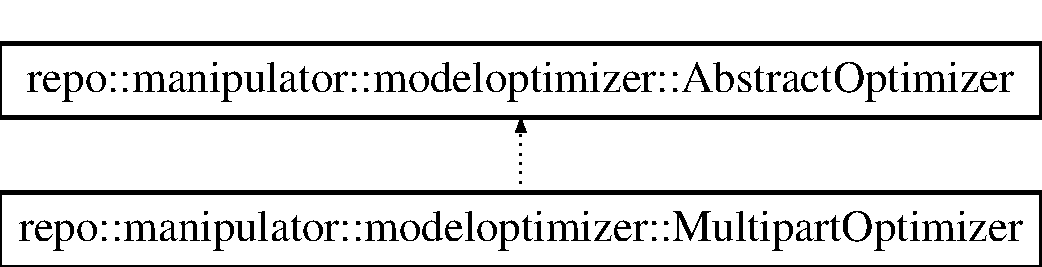
\includegraphics[height=2.000000cm]{classrepo_1_1manipulator_1_1modeloptimizer_1_1_multipart_optimizer}
\end{center}
\end{figure}
\subsection*{Public Member Functions}
\begin{DoxyCompactItemize}
\item 
\hyperlink{classrepo_1_1manipulator_1_1modeloptimizer_1_1_multipart_optimizer_a2f4e43f341ec4badbc60ce51499ed0ab}{Multipart\+Optimizer} ()
\item 
virtual \hyperlink{classrepo_1_1manipulator_1_1modeloptimizer_1_1_multipart_optimizer_a9e7354058021e00d6d75e63eef3b57cd}{$\sim$\+Multipart\+Optimizer} ()
\item 
bool \hyperlink{classrepo_1_1manipulator_1_1modeloptimizer_1_1_multipart_optimizer_a3e223c461f5b27c09f9037a57ff3fd01}{apply} (\hyperlink{classrepo_1_1core_1_1model_1_1_repo_scene}{repo\+::core\+::model\+::\+Repo\+Scene} $\ast$scene)
\end{DoxyCompactItemize}


\subsection{Constructor \& Destructor Documentation}
\hypertarget{classrepo_1_1manipulator_1_1modeloptimizer_1_1_multipart_optimizer_a2f4e43f341ec4badbc60ce51499ed0ab}{}\index{repo\+::manipulator\+::modeloptimizer\+::\+Multipart\+Optimizer@{repo\+::manipulator\+::modeloptimizer\+::\+Multipart\+Optimizer}!Multipart\+Optimizer@{Multipart\+Optimizer}}
\index{Multipart\+Optimizer@{Multipart\+Optimizer}!repo\+::manipulator\+::modeloptimizer\+::\+Multipart\+Optimizer@{repo\+::manipulator\+::modeloptimizer\+::\+Multipart\+Optimizer}}
\subsubsection[{Multipart\+Optimizer}]{\setlength{\rightskip}{0pt plus 5cm}Multipart\+Optimizer\+::\+Multipart\+Optimizer (
\begin{DoxyParamCaption}
{}
\end{DoxyParamCaption}
)}\label{classrepo_1_1manipulator_1_1modeloptimizer_1_1_multipart_optimizer_a2f4e43f341ec4badbc60ce51499ed0ab}
Default constructor \hypertarget{classrepo_1_1manipulator_1_1modeloptimizer_1_1_multipart_optimizer_a9e7354058021e00d6d75e63eef3b57cd}{}\index{repo\+::manipulator\+::modeloptimizer\+::\+Multipart\+Optimizer@{repo\+::manipulator\+::modeloptimizer\+::\+Multipart\+Optimizer}!````~Multipart\+Optimizer@{$\sim$\+Multipart\+Optimizer}}
\index{````~Multipart\+Optimizer@{$\sim$\+Multipart\+Optimizer}!repo\+::manipulator\+::modeloptimizer\+::\+Multipart\+Optimizer@{repo\+::manipulator\+::modeloptimizer\+::\+Multipart\+Optimizer}}
\subsubsection[{$\sim$\+Multipart\+Optimizer}]{\setlength{\rightskip}{0pt plus 5cm}Multipart\+Optimizer\+::$\sim$\+Multipart\+Optimizer (
\begin{DoxyParamCaption}
{}
\end{DoxyParamCaption}
)\hspace{0.3cm}{\ttfamily [virtual]}}\label{classrepo_1_1manipulator_1_1modeloptimizer_1_1_multipart_optimizer_a9e7354058021e00d6d75e63eef3b57cd}
Default deconstructor 

\subsection{Member Function Documentation}
\hypertarget{classrepo_1_1manipulator_1_1modeloptimizer_1_1_multipart_optimizer_a3e223c461f5b27c09f9037a57ff3fd01}{}\index{repo\+::manipulator\+::modeloptimizer\+::\+Multipart\+Optimizer@{repo\+::manipulator\+::modeloptimizer\+::\+Multipart\+Optimizer}!apply@{apply}}
\index{apply@{apply}!repo\+::manipulator\+::modeloptimizer\+::\+Multipart\+Optimizer@{repo\+::manipulator\+::modeloptimizer\+::\+Multipart\+Optimizer}}
\subsubsection[{apply}]{\setlength{\rightskip}{0pt plus 5cm}bool Multipart\+Optimizer\+::apply (
\begin{DoxyParamCaption}
\item[{{\bf repo\+::core\+::model\+::\+Repo\+Scene} $\ast$}]{scene}
\end{DoxyParamCaption}
)\hspace{0.3cm}{\ttfamily [virtual]}}\label{classrepo_1_1manipulator_1_1modeloptimizer_1_1_multipart_optimizer_a3e223c461f5b27c09f9037a57ff3fd01}
Apply optimisation on the given repo\+Scene 
\begin{DoxyParams}{Parameters}
{\em scene} & takes in a repo\+Scene to optimise \\
\hline
\end{DoxyParams}
\begin{DoxyReturn}{Returns}
returns true upon success 
\end{DoxyReturn}


Implements \hyperlink{classrepo_1_1manipulator_1_1modeloptimizer_1_1_abstract_optimizer_a38e98344c1d3c66fbea8adae41dc6cb1}{repo\+::manipulator\+::modeloptimizer\+::\+Abstract\+Optimizer}.



The documentation for this class was generated from the following files\+:\begin{DoxyCompactItemize}
\item 
C\+:/\+Users/\+Carmen/3\+D Repo/\+Repo/3drepobouncer/bouncer/src/repo/manipulator/modeloptimizer/repo\+\_\+optimizer\+\_\+multipart.\+h\item 
C\+:/\+Users/\+Carmen/3\+D Repo/\+Repo/3drepobouncer/bouncer/src/repo/manipulator/modeloptimizer/repo\+\_\+optimizer\+\_\+multipart.\+cpp\end{DoxyCompactItemize}

\hypertarget{classrepo_1_1lib_1_1_property_tree}{}\section{repo\+:\+:lib\+:\+:Property\+Tree Class Reference}
\label{classrepo_1_1lib_1_1_property_tree}\index{repo\+::lib\+::\+Property\+Tree@{repo\+::lib\+::\+Property\+Tree}}
\subsection*{Public Member Functions}
\begin{DoxyCompactItemize}
\item 
\hypertarget{classrepo_1_1lib_1_1_property_tree_a6b9bba9357c593e3f5078782a9cdfb3d}{}{\bfseries Property\+Tree} (const bool \&enable\+J\+S\+O\+N\+Work\+Around)\label{classrepo_1_1lib_1_1_property_tree_a6b9bba9357c593e3f5078782a9cdfb3d}

\item 
void \hyperlink{classrepo_1_1lib_1_1_property_tree_afede341c65d0add71623545e123170ef}{add\+Array\+Objects} (const std\+::string \&label, const std\+::vector$<$ \hyperlink{classrepo_1_1lib_1_1_property_tree}{Property\+Tree} $>$ \&value)
\item 
{\footnotesize template$<$typename T $>$ }\\void \hyperlink{classrepo_1_1lib_1_1_property_tree_a5f27875958fdc8b1e0434a6d73ba2b1a}{add\+Field\+Attribute} (const std\+::string \&label, const std\+::string \&attribute, const T \&value)
\item 
{\footnotesize template$<$typename T $>$ }\\void \hyperlink{classrepo_1_1lib_1_1_property_tree_aa63cfcbb32ddb2d7b73609b929379676}{add\+Field\+Attribute} (const std\+::string \&label, const std\+::string \&attribute, const std\+::vector$<$ T $>$ \&value, const bool \&use\+Delimiter=true)
\item 
{\footnotesize template$<$typename T $>$ }\\void \hyperlink{classrepo_1_1lib_1_1_property_tree_a79fae0e843120797f2eca9a8dc5d9eba}{add\+To\+Tree} (const std\+::string \&label, const T \&value)
\item 
\hypertarget{classrepo_1_1lib_1_1_property_tree_a9c85a9eec0431b10d760f29a1c5c9615}{}{\footnotesize template$<$std\+::size\+\_\+t N$>$ }\\void {\bfseries add\+To\+Tree} (const std\+::string \&label, const char(\&value)\mbox{[}N\mbox{]})\label{classrepo_1_1lib_1_1_property_tree_a9c85a9eec0431b10d760f29a1c5c9615}

\item 
{\footnotesize template$<$typename T $>$ }\\void \hyperlink{classrepo_1_1lib_1_1_property_tree_aff24090893254b6bacb4a87a3dc463b1}{add\+To\+Tree} (const std\+::string \&label, const std\+::vector$<$ T $>$ \&value, const bool \&join=true)
\item 
void \hyperlink{classrepo_1_1lib_1_1_property_tree_ac830c1a733589cb5add54a7894dc9417}{disable\+J\+S\+O\+N\+Workaround} ()
\item 
void \hyperlink{classrepo_1_1lib_1_1_property_tree_ace335b74ffb3d113d44cdc92ebd83121}{merge\+Sub\+Tree} (const std\+::string \&label, const \hyperlink{classrepo_1_1lib_1_1_property_tree}{Property\+Tree} \&sub\+Tree)
\item 
void \hyperlink{classrepo_1_1lib_1_1_property_tree_a7839bcc54f771858ef1d046cea234cce}{write\+\_\+json} (std\+::iostream \&stream) const 
\item 
void \hyperlink{classrepo_1_1lib_1_1_property_tree_a22397eaf6fe50716a5a99c64dbde2294}{write\+\_\+xml} (std\+::iostream \&stream) const 
\item 
\hypertarget{classrepo_1_1lib_1_1_property_tree_a5bc49d8b8e5f5cac2e6cf921cd1c2874}{}{\footnotesize template$<$$>$ }\\void {\bfseries add\+Field\+Attribute} (const std\+::string \&label, const std\+::string \&attribute, const std\+::string \&value)\label{classrepo_1_1lib_1_1_property_tree_a5bc49d8b8e5f5cac2e6cf921cd1c2874}

\item 
\hypertarget{classrepo_1_1lib_1_1_property_tree_af3e02bc7144d85e6e39e2d2f1cfe8eb1}{}{\footnotesize template$<$$>$ }\\void {\bfseries add\+Field\+Attribute} (const std\+::string \&label, const std\+::string \&attribute, const \hyperlink{structrepo__vector__t}{repo\+\_\+vector\+\_\+t} \&value)\label{classrepo_1_1lib_1_1_property_tree_af3e02bc7144d85e6e39e2d2f1cfe8eb1}

\item 
\hypertarget{classrepo_1_1lib_1_1_property_tree_a48c7654533f0ae36866ea4b373760396}{}{\footnotesize template$<$$>$ }\\void {\bfseries add\+To\+Tree} (const std\+::string \&label, const repo\+U\+U\+I\+D \&value)\label{classrepo_1_1lib_1_1_property_tree_a48c7654533f0ae36866ea4b373760396}

\item 
\hypertarget{classrepo_1_1lib_1_1_property_tree_aae4dc92fcc99e294066995f2f2499de2}{}{\footnotesize template$<$$>$ }\\void {\bfseries add\+To\+Tree} (const std\+::string \&label, const \hyperlink{structrepo__vector__t}{repo\+\_\+vector\+\_\+t} \&value)\label{classrepo_1_1lib_1_1_property_tree_aae4dc92fcc99e294066995f2f2499de2}

\item 
\hypertarget{classrepo_1_1lib_1_1_property_tree_a1b11948aef1f85a44adc3153168a08cb}{}{\footnotesize template$<$$>$ }\\void {\bfseries add\+To\+Tree} (const std\+::string \&label, const std\+::vector$<$ \hyperlink{classrepo_1_1lib_1_1_property_tree}{Property\+Tree} $>$ \&value, const bool \&join)\label{classrepo_1_1lib_1_1_property_tree_a1b11948aef1f85a44adc3153168a08cb}

\item 
\hypertarget{classrepo_1_1lib_1_1_property_tree_aae4dc92fcc99e294066995f2f2499de2}{}{\footnotesize template$<$$>$ }\\void {\bfseries add\+To\+Tree} (const std\+::string \&label, const \hyperlink{structrepo__vector__t}{repo\+\_\+vector\+\_\+t} \&value)\label{classrepo_1_1lib_1_1_property_tree_aae4dc92fcc99e294066995f2f2499de2}

\item 
\hypertarget{classrepo_1_1lib_1_1_property_tree_a48c7654533f0ae36866ea4b373760396}{}{\footnotesize template$<$$>$ }\\void {\bfseries add\+To\+Tree} (const std\+::string \&label, const repo\+U\+U\+I\+D \&value)\label{classrepo_1_1lib_1_1_property_tree_a48c7654533f0ae36866ea4b373760396}

\end{DoxyCompactItemize}


\subsection{Member Function Documentation}
\hypertarget{classrepo_1_1lib_1_1_property_tree_afede341c65d0add71623545e123170ef}{}\index{repo\+::lib\+::\+Property\+Tree@{repo\+::lib\+::\+Property\+Tree}!add\+Array\+Objects@{add\+Array\+Objects}}
\index{add\+Array\+Objects@{add\+Array\+Objects}!repo\+::lib\+::\+Property\+Tree@{repo\+::lib\+::\+Property\+Tree}}
\subsubsection[{add\+Array\+Objects}]{\setlength{\rightskip}{0pt plus 5cm}void repo\+::lib\+::\+Property\+Tree\+::add\+Array\+Objects (
\begin{DoxyParamCaption}
\item[{const std\+::string \&}]{label, }
\item[{const std\+::vector$<$ {\bf Property\+Tree} $>$ \&}]{value}
\end{DoxyParamCaption}
)\hspace{0.3cm}{\ttfamily [inline]}}\label{classrepo_1_1lib_1_1_property_tree_afede341c65d0add71623545e123170ef}
Add an array of objects to the tree at a specified level This is used for things like arrays of objects within J\+S\+O\+N 
\begin{DoxyParams}{Parameters}
{\em label} & indicating where the child lives in the tree \\
\hline
{\em value} & vector of children to add \\
\hline
\end{DoxyParams}
\hypertarget{classrepo_1_1lib_1_1_property_tree_a5f27875958fdc8b1e0434a6d73ba2b1a}{}\index{repo\+::lib\+::\+Property\+Tree@{repo\+::lib\+::\+Property\+Tree}!add\+Field\+Attribute@{add\+Field\+Attribute}}
\index{add\+Field\+Attribute@{add\+Field\+Attribute}!repo\+::lib\+::\+Property\+Tree@{repo\+::lib\+::\+Property\+Tree}}
\subsubsection[{add\+Field\+Attribute}]{\setlength{\rightskip}{0pt plus 5cm}template$<$typename T $>$ void repo\+::lib\+::\+Property\+Tree\+::add\+Field\+Attribute (
\begin{DoxyParamCaption}
\item[{const std\+::string \&}]{label, }
\item[{const std\+::string \&}]{attribute, }
\item[{const T \&}]{value}
\end{DoxyParamCaption}
)\hspace{0.3cm}{\ttfamily [inline]}}\label{classrepo_1_1lib_1_1_property_tree_a5f27875958fdc8b1e0434a6d73ba2b1a}
Add an attribute to the field This is very xml specific it is to achieve things like $<$\+F\+I\+E\+L\+D name=\char`\"{}\+Hi\char`\"{}$>$ instead of $<$\+F\+I\+E\+L\+D$>$\char`\"{}\+Hi\char`\"{}$<$/\+F\+I\+E\+L\+D$>$ The type fo the value can be of any type as long as it is a qualified member of std\+::to\+\_\+string() 
\begin{DoxyParams}{Parameters}
{\em label} & field name to add to \\
\hline
{\em attribute} & name of attribute \\
\hline
{\em value} & value of attribute \\
\hline
\end{DoxyParams}
\hypertarget{classrepo_1_1lib_1_1_property_tree_aa63cfcbb32ddb2d7b73609b929379676}{}\index{repo\+::lib\+::\+Property\+Tree@{repo\+::lib\+::\+Property\+Tree}!add\+Field\+Attribute@{add\+Field\+Attribute}}
\index{add\+Field\+Attribute@{add\+Field\+Attribute}!repo\+::lib\+::\+Property\+Tree@{repo\+::lib\+::\+Property\+Tree}}
\subsubsection[{add\+Field\+Attribute}]{\setlength{\rightskip}{0pt plus 5cm}template$<$typename T $>$ void repo\+::lib\+::\+Property\+Tree\+::add\+Field\+Attribute (
\begin{DoxyParamCaption}
\item[{const std\+::string \&}]{label, }
\item[{const std\+::string \&}]{attribute, }
\item[{const std\+::vector$<$ T $>$ \&}]{value, }
\item[{const bool \&}]{use\+Delimiter = {\ttfamily true}}
\end{DoxyParamCaption}
)\hspace{0.3cm}{\ttfamily [inline]}}\label{classrepo_1_1lib_1_1_property_tree_aa63cfcbb32ddb2d7b73609b929379676}
Add an attribute to the field This is very xml specific it is to achieve things like $<$\+F\+I\+E\+L\+D name=\char`\"{}\+Hi\char`\"{}$>$ instead of $<$\+F\+I\+E\+L\+D$>$\char`\"{}\+Hi\char`\"{}$<$/\+F\+I\+E\+L\+D$>$ The type of the vector can be of any type as long as it is a qualified member of std\+::to\+\_\+string() 
\begin{DoxyParams}{Parameters}
{\em label} & field name to add to \\
\hline
{\em attribute} & name of attribute \\
\hline
{\em value} & value of attribute \\
\hline
\end{DoxyParams}
\hypertarget{classrepo_1_1lib_1_1_property_tree_a79fae0e843120797f2eca9a8dc5d9eba}{}\index{repo\+::lib\+::\+Property\+Tree@{repo\+::lib\+::\+Property\+Tree}!add\+To\+Tree@{add\+To\+Tree}}
\index{add\+To\+Tree@{add\+To\+Tree}!repo\+::lib\+::\+Property\+Tree@{repo\+::lib\+::\+Property\+Tree}}
\subsubsection[{add\+To\+Tree}]{\setlength{\rightskip}{0pt plus 5cm}template$<$typename T $>$ void repo\+::lib\+::\+Property\+Tree\+::add\+To\+Tree (
\begin{DoxyParamCaption}
\item[{const std\+::string \&}]{label, }
\item[{const T \&}]{value}
\end{DoxyParamCaption}
)\hspace{0.3cm}{\ttfamily [inline]}}\label{classrepo_1_1lib_1_1_property_tree_a79fae0e843120797f2eca9a8dc5d9eba}
Add a children onto the tree label can denote it\textquotesingle{}s inheritance. for e.\+g. trunk.\+branch.\+leaf would denote the child name is leaf, with parent branch and grandparent trunk. 
\begin{DoxyParams}{Parameters}
{\em label} & indicating where the child lives in the tree \\
\hline
{\em value} & value of the children \\
\hline
\end{DoxyParams}
\hypertarget{classrepo_1_1lib_1_1_property_tree_aff24090893254b6bacb4a87a3dc463b1}{}\index{repo\+::lib\+::\+Property\+Tree@{repo\+::lib\+::\+Property\+Tree}!add\+To\+Tree@{add\+To\+Tree}}
\index{add\+To\+Tree@{add\+To\+Tree}!repo\+::lib\+::\+Property\+Tree@{repo\+::lib\+::\+Property\+Tree}}
\subsubsection[{add\+To\+Tree}]{\setlength{\rightskip}{0pt plus 5cm}template$<$typename T $>$ void repo\+::lib\+::\+Property\+Tree\+::add\+To\+Tree (
\begin{DoxyParamCaption}
\item[{const std\+::string \&}]{label, }
\item[{const std\+::vector$<$ T $>$ \&}]{value, }
\item[{const bool \&}]{join = {\ttfamily true}}
\end{DoxyParamCaption}
)\hspace{0.3cm}{\ttfamily [inline]}}\label{classrepo_1_1lib_1_1_property_tree_aff24090893254b6bacb4a87a3dc463b1}
Add an array of values to the tree at a specified level This is used for things like arrays within J\+S\+O\+N 
\begin{DoxyParams}{Parameters}
{\em label} & indicating where the child lives in the tree \\
\hline
{\em value} & vector of children to add \\
\hline
{\em join} & merge vector into a string value instead of putting in a vector \\
\hline
\end{DoxyParams}
\hypertarget{classrepo_1_1lib_1_1_property_tree_ac830c1a733589cb5add54a7894dc9417}{}\index{repo\+::lib\+::\+Property\+Tree@{repo\+::lib\+::\+Property\+Tree}!disable\+J\+S\+O\+N\+Workaround@{disable\+J\+S\+O\+N\+Workaround}}
\index{disable\+J\+S\+O\+N\+Workaround@{disable\+J\+S\+O\+N\+Workaround}!repo\+::lib\+::\+Property\+Tree@{repo\+::lib\+::\+Property\+Tree}}
\subsubsection[{disable\+J\+S\+O\+N\+Workaround}]{\setlength{\rightskip}{0pt plus 5cm}void repo\+::lib\+::\+Property\+Tree\+::disable\+J\+S\+O\+N\+Workaround (
\begin{DoxyParamCaption}
{}
\end{DoxyParamCaption}
)\hspace{0.3cm}{\ttfamily [inline]}}\label{classrepo_1_1lib_1_1_property_tree_ac830c1a733589cb5add54a7894dc9417}
Disable the J\+S\+O\+N workaround for quotes There is currently a work around to allow json parser writes to remove quotes from anything that isn\textquotesingle{}t a string. Calling this function will disable it. You might want to do this B\+E\+F\+O\+R\+E you add any data into the tree for X\+M\+L or any non J\+S\+O\+N exports \hypertarget{classrepo_1_1lib_1_1_property_tree_ace335b74ffb3d113d44cdc92ebd83121}{}\index{repo\+::lib\+::\+Property\+Tree@{repo\+::lib\+::\+Property\+Tree}!merge\+Sub\+Tree@{merge\+Sub\+Tree}}
\index{merge\+Sub\+Tree@{merge\+Sub\+Tree}!repo\+::lib\+::\+Property\+Tree@{repo\+::lib\+::\+Property\+Tree}}
\subsubsection[{merge\+Sub\+Tree}]{\setlength{\rightskip}{0pt plus 5cm}void repo\+::lib\+::\+Property\+Tree\+::merge\+Sub\+Tree (
\begin{DoxyParamCaption}
\item[{const std\+::string \&}]{label, }
\item[{const {\bf Property\+Tree} \&}]{sub\+Tree}
\end{DoxyParamCaption}
)\hspace{0.3cm}{\ttfamily [inline]}}\label{classrepo_1_1lib_1_1_property_tree_ace335b74ffb3d113d44cdc92ebd83121}
Merging sub tree into this tree 
\begin{DoxyParams}{Parameters}
{\em label} & label where the sub\+Tree goes \\
\hline
{\em sub\+Tree} & the sub tree to add \\
\hline
\end{DoxyParams}
\hypertarget{classrepo_1_1lib_1_1_property_tree_a7839bcc54f771858ef1d046cea234cce}{}\index{repo\+::lib\+::\+Property\+Tree@{repo\+::lib\+::\+Property\+Tree}!write\+\_\+json@{write\+\_\+json}}
\index{write\+\_\+json@{write\+\_\+json}!repo\+::lib\+::\+Property\+Tree@{repo\+::lib\+::\+Property\+Tree}}
\subsubsection[{write\+\_\+json}]{\setlength{\rightskip}{0pt plus 5cm}void repo\+::lib\+::\+Property\+Tree\+::write\+\_\+json (
\begin{DoxyParamCaption}
\item[{std\+::iostream \&}]{stream}
\end{DoxyParamCaption}
) const\hspace{0.3cm}{\ttfamily [inline]}}\label{classrepo_1_1lib_1_1_property_tree_a7839bcc54f771858ef1d046cea234cce}
Write tree data onto a stream 
\begin{DoxyParams}{Parameters}
{\em stream} & stream to write onto \\
\hline
\end{DoxyParams}
\hypertarget{classrepo_1_1lib_1_1_property_tree_a22397eaf6fe50716a5a99c64dbde2294}{}\index{repo\+::lib\+::\+Property\+Tree@{repo\+::lib\+::\+Property\+Tree}!write\+\_\+xml@{write\+\_\+xml}}
\index{write\+\_\+xml@{write\+\_\+xml}!repo\+::lib\+::\+Property\+Tree@{repo\+::lib\+::\+Property\+Tree}}
\subsubsection[{write\+\_\+xml}]{\setlength{\rightskip}{0pt plus 5cm}void repo\+::lib\+::\+Property\+Tree\+::write\+\_\+xml (
\begin{DoxyParamCaption}
\item[{std\+::iostream \&}]{stream}
\end{DoxyParamCaption}
) const\hspace{0.3cm}{\ttfamily [inline]}}\label{classrepo_1_1lib_1_1_property_tree_a22397eaf6fe50716a5a99c64dbde2294}
Write tree data onto a stream 
\begin{DoxyParams}{Parameters}
{\em stream} & stream to write onto \\
\hline
\end{DoxyParams}


The documentation for this class was generated from the following files\+:\begin{DoxyCompactItemize}
\item 
C\+:/\+Users/\+Carmen/3\+D Repo/\+Repo/3drepobouncer/bouncer/src/repo/lib/repo\+\_\+property\+\_\+tree.\+h\item 
C\+:/\+Users/\+Carmen/3\+D Repo/\+Repo/3drepobouncer/bouncer/src/repo/lib/repo\+\_\+property\+\_\+tree.\+cpp\end{DoxyCompactItemize}

\hypertarget{classrepo_1_1manipulator_1_1modelutility_1_1_r_d_tree_spatial_partitioner}{}\section{repo\+:\+:manipulator\+:\+:modelutility\+:\+:R\+D\+Tree\+Spatial\+Partitioner Class Reference}
\label{classrepo_1_1manipulator_1_1modelutility_1_1_r_d_tree_spatial_partitioner}\index{repo\+::manipulator\+::modelutility\+::\+R\+D\+Tree\+Spatial\+Partitioner@{repo\+::manipulator\+::modelutility\+::\+R\+D\+Tree\+Spatial\+Partitioner}}
Inheritance diagram for repo\+:\+:manipulator\+:\+:modelutility\+:\+:R\+D\+Tree\+Spatial\+Partitioner\+:\begin{figure}[H]
\begin{center}
\leavevmode
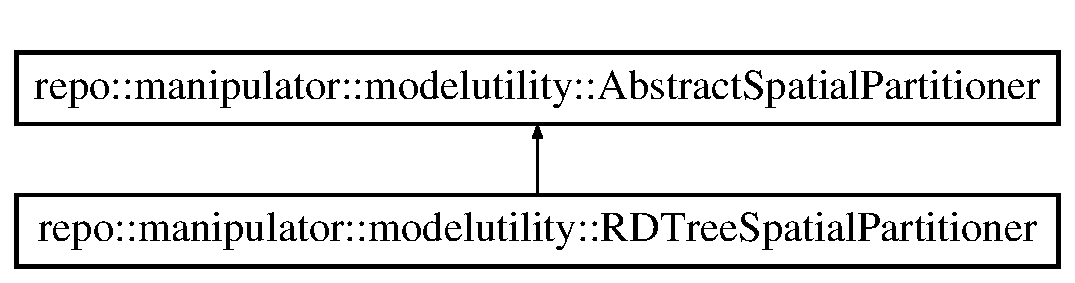
\includegraphics[height=2.000000cm]{classrepo_1_1manipulator_1_1modelutility_1_1_r_d_tree_spatial_partitioner}
\end{center}
\end{figure}
\subsection*{Public Member Functions}
\begin{DoxyCompactItemize}
\item 
\hyperlink{classrepo_1_1manipulator_1_1modelutility_1_1_r_d_tree_spatial_partitioner_a4a6e0cdf7349cb359a867c1aceb709f1}{R\+D\+Tree\+Spatial\+Partitioner} (const \hyperlink{classrepo_1_1core_1_1model_1_1_repo_scene}{repo\+::core\+::model\+::\+Repo\+Scene} $\ast$scene, const uint32\+\_\+t \&max\+Depth=12)
\item 
virtual std\+::shared\+\_\+ptr$<$ \hyperlink{structrepo__partitioning__tree__t}{repo\+\_\+partitioning\+\_\+tree\+\_\+t} $>$ \hyperlink{classrepo_1_1manipulator_1_1modelutility_1_1_r_d_tree_spatial_partitioner_a768852ef54d357e43b86a70897002623}{partition\+Scene} ()
\end{DoxyCompactItemize}
\subsection*{Protected Member Functions}
\begin{DoxyCompactItemize}
\item 
std\+::vector$<$ \hyperlink{structrepo__mesh__entry__t}{repo\+\_\+mesh\+\_\+entry\+\_\+t} $>$ \hyperlink{classrepo_1_1manipulator_1_1modelutility_1_1_r_d_tree_spatial_partitioner_a86a33d1ea3b1c82606d4542d3cd82de3}{create\+Mesh\+Entries} ()
\item 
std\+::shared\+\_\+ptr$<$ \hyperlink{structrepo__partitioning__tree__t}{repo\+\_\+partitioning\+\_\+tree\+\_\+t} $>$ \hyperlink{classrepo_1_1manipulator_1_1modelutility_1_1_r_d_tree_spatial_partitioner_ad4b1863028ddec9a1e50b083a4ec656e}{create\+Partition} (const std\+::vector$<$ \hyperlink{structrepo__mesh__entry__t}{repo\+\_\+mesh\+\_\+entry\+\_\+t} $>$ \&meshes, const repo\+::\+Partitioning\+Tree\+Type \&axis, const uint32\+\_\+t \&depth\+Count, const uint32\+\_\+t \&failcount, const std\+::vector$<$ std\+::vector$<$ float $>$$>$ \&current\+Section)
\item 
void \hyperlink{classrepo_1_1manipulator_1_1modelutility_1_1_r_d_tree_spatial_partitioner_ada2a7684178144f06dfea923647ae9e8}{sort\+Meshes} (const std\+::vector$<$ \hyperlink{structrepo__mesh__entry__t}{repo\+\_\+mesh\+\_\+entry\+\_\+t} $>$ \&meshes, const repo\+::\+Partitioning\+Tree\+Type \&axis, const std\+::vector$<$ std\+::vector$<$ float $>$$>$ \&current\+Section, float \&median, std\+::vector$<$ \hyperlink{structrepo__mesh__entry__t}{repo\+\_\+mesh\+\_\+entry\+\_\+t} $>$ \&l\+Meshes, std\+::vector$<$ \hyperlink{structrepo__mesh__entry__t}{repo\+\_\+mesh\+\_\+entry\+\_\+t} $>$ \&r\+Meshes)
\end{DoxyCompactItemize}
\subsection*{Additional Inherited Members}


\subsection{Constructor \& Destructor Documentation}
\hypertarget{classrepo_1_1manipulator_1_1modelutility_1_1_r_d_tree_spatial_partitioner_a4a6e0cdf7349cb359a867c1aceb709f1}{}\index{repo\+::manipulator\+::modelutility\+::\+R\+D\+Tree\+Spatial\+Partitioner@{repo\+::manipulator\+::modelutility\+::\+R\+D\+Tree\+Spatial\+Partitioner}!R\+D\+Tree\+Spatial\+Partitioner@{R\+D\+Tree\+Spatial\+Partitioner}}
\index{R\+D\+Tree\+Spatial\+Partitioner@{R\+D\+Tree\+Spatial\+Partitioner}!repo\+::manipulator\+::modelutility\+::\+R\+D\+Tree\+Spatial\+Partitioner@{repo\+::manipulator\+::modelutility\+::\+R\+D\+Tree\+Spatial\+Partitioner}}
\subsubsection[{R\+D\+Tree\+Spatial\+Partitioner}]{\setlength{\rightskip}{0pt plus 5cm}R\+D\+Tree\+Spatial\+Partitioner\+::\+R\+D\+Tree\+Spatial\+Partitioner (
\begin{DoxyParamCaption}
\item[{const {\bf repo\+::core\+::model\+::\+Repo\+Scene} $\ast$}]{scene, }
\item[{const uint32\+\_\+t \&}]{max\+Depth = {\ttfamily 12}}
\end{DoxyParamCaption}
)}\label{classrepo_1_1manipulator_1_1modelutility_1_1_r_d_tree_spatial_partitioner_a4a6e0cdf7349cb359a867c1aceb709f1}
R\+D Tree Spatial Partitioning utility class to spatially divide a scene graph base on its meshes This algorithm will produce an R\+D Tree with it it\textquotesingle{}s partitioning value determined by the median value of min bounding boxes. Note\+: currently only support scene with optimised graph! 
\begin{DoxyParams}{Parameters}
{\em scene} & scene to divide \\
\hline
{\em depth} & limiting depth of the tree (0 to disable limitation) \\
\hline
\end{DoxyParams}


\subsection{Member Function Documentation}
\hypertarget{classrepo_1_1manipulator_1_1modelutility_1_1_r_d_tree_spatial_partitioner_a86a33d1ea3b1c82606d4542d3cd82de3}{}\index{repo\+::manipulator\+::modelutility\+::\+R\+D\+Tree\+Spatial\+Partitioner@{repo\+::manipulator\+::modelutility\+::\+R\+D\+Tree\+Spatial\+Partitioner}!create\+Mesh\+Entries@{create\+Mesh\+Entries}}
\index{create\+Mesh\+Entries@{create\+Mesh\+Entries}!repo\+::manipulator\+::modelutility\+::\+R\+D\+Tree\+Spatial\+Partitioner@{repo\+::manipulator\+::modelutility\+::\+R\+D\+Tree\+Spatial\+Partitioner}}
\subsubsection[{create\+Mesh\+Entries}]{\setlength{\rightskip}{0pt plus 5cm}std\+::vector$<$ {\bf repo\+\_\+mesh\+\_\+entry\+\_\+t} $>$ R\+D\+Tree\+Spatial\+Partitioner\+::create\+Mesh\+Entries (
\begin{DoxyParamCaption}
{}
\end{DoxyParamCaption}
)\hspace{0.3cm}{\ttfamily [protected]}}\label{classrepo_1_1manipulator_1_1modelutility_1_1_r_d_tree_spatial_partitioner_a86a33d1ea3b1c82606d4542d3cd82de3}
Generate a vector of mesh entries base on the current scene. \hypertarget{classrepo_1_1manipulator_1_1modelutility_1_1_r_d_tree_spatial_partitioner_ad4b1863028ddec9a1e50b083a4ec656e}{}\index{repo\+::manipulator\+::modelutility\+::\+R\+D\+Tree\+Spatial\+Partitioner@{repo\+::manipulator\+::modelutility\+::\+R\+D\+Tree\+Spatial\+Partitioner}!create\+Partition@{create\+Partition}}
\index{create\+Partition@{create\+Partition}!repo\+::manipulator\+::modelutility\+::\+R\+D\+Tree\+Spatial\+Partitioner@{repo\+::manipulator\+::modelutility\+::\+R\+D\+Tree\+Spatial\+Partitioner}}
\subsubsection[{create\+Partition}]{\setlength{\rightskip}{0pt plus 5cm}std\+::shared\+\_\+ptr$<$ {\bf repo\+\_\+partitioning\+\_\+tree\+\_\+t} $>$ R\+D\+Tree\+Spatial\+Partitioner\+::create\+Partition (
\begin{DoxyParamCaption}
\item[{const std\+::vector$<$ {\bf repo\+\_\+mesh\+\_\+entry\+\_\+t} $>$ \&}]{meshes, }
\item[{const repo\+::\+Partitioning\+Tree\+Type \&}]{axis, }
\item[{const uint32\+\_\+t \&}]{depth\+Count, }
\item[{const uint32\+\_\+t \&}]{failcount, }
\item[{const std\+::vector$<$ std\+::vector$<$ float $>$$>$ \&}]{current\+Section}
\end{DoxyParamCaption}
)\hspace{0.3cm}{\ttfamily [protected]}}\label{classrepo_1_1manipulator_1_1modelutility_1_1_r_d_tree_spatial_partitioner_ad4b1863028ddec9a1e50b083a4ec656e}
Create a partitioning with the given meshes 
\begin{DoxyParams}{Parameters}
{\em meshes} & meshes to divide \\
\hline
{\em axis} & which axis to divide \\
\hline
{\em depth\+Count} & current depth \\
\hline
\end{DoxyParams}
\hypertarget{classrepo_1_1manipulator_1_1modelutility_1_1_r_d_tree_spatial_partitioner_a768852ef54d357e43b86a70897002623}{}\index{repo\+::manipulator\+::modelutility\+::\+R\+D\+Tree\+Spatial\+Partitioner@{repo\+::manipulator\+::modelutility\+::\+R\+D\+Tree\+Spatial\+Partitioner}!partition\+Scene@{partition\+Scene}}
\index{partition\+Scene@{partition\+Scene}!repo\+::manipulator\+::modelutility\+::\+R\+D\+Tree\+Spatial\+Partitioner@{repo\+::manipulator\+::modelutility\+::\+R\+D\+Tree\+Spatial\+Partitioner}}
\subsubsection[{partition\+Scene}]{\setlength{\rightskip}{0pt plus 5cm}std\+::shared\+\_\+ptr$<$ {\bf repo\+\_\+partitioning\+\_\+tree\+\_\+t} $>$ R\+D\+Tree\+Spatial\+Partitioner\+::partition\+Scene (
\begin{DoxyParamCaption}
{}
\end{DoxyParamCaption}
)\hspace{0.3cm}{\ttfamily [virtual]}}\label{classrepo_1_1manipulator_1_1modelutility_1_1_r_d_tree_spatial_partitioner_a768852ef54d357e43b86a70897002623}
Partition the scene \begin{DoxyReturn}{Returns}
returns the spatial partitioning information as a tree 
\end{DoxyReturn}


Implements \hyperlink{classrepo_1_1manipulator_1_1modelutility_1_1_abstract_spatial_partitioner_af1e6e3540698ff0f4ec52cd758260aba}{repo\+::manipulator\+::modelutility\+::\+Abstract\+Spatial\+Partitioner}.

\hypertarget{classrepo_1_1manipulator_1_1modelutility_1_1_r_d_tree_spatial_partitioner_ada2a7684178144f06dfea923647ae9e8}{}\index{repo\+::manipulator\+::modelutility\+::\+R\+D\+Tree\+Spatial\+Partitioner@{repo\+::manipulator\+::modelutility\+::\+R\+D\+Tree\+Spatial\+Partitioner}!sort\+Meshes@{sort\+Meshes}}
\index{sort\+Meshes@{sort\+Meshes}!repo\+::manipulator\+::modelutility\+::\+R\+D\+Tree\+Spatial\+Partitioner@{repo\+::manipulator\+::modelutility\+::\+R\+D\+Tree\+Spatial\+Partitioner}}
\subsubsection[{sort\+Meshes}]{\setlength{\rightskip}{0pt plus 5cm}void R\+D\+Tree\+Spatial\+Partitioner\+::sort\+Meshes (
\begin{DoxyParamCaption}
\item[{const std\+::vector$<$ {\bf repo\+\_\+mesh\+\_\+entry\+\_\+t} $>$ \&}]{meshes, }
\item[{const repo\+::\+Partitioning\+Tree\+Type \&}]{axis, }
\item[{const std\+::vector$<$ std\+::vector$<$ float $>$$>$ \&}]{current\+Section, }
\item[{float \&}]{median, }
\item[{std\+::vector$<$ {\bf repo\+\_\+mesh\+\_\+entry\+\_\+t} $>$ \&}]{l\+Meshes, }
\item[{std\+::vector$<$ {\bf repo\+\_\+mesh\+\_\+entry\+\_\+t} $>$ \&}]{r\+Meshes}
\end{DoxyParamCaption}
)\hspace{0.3cm}{\ttfamily [protected]}}\label{classrepo_1_1manipulator_1_1modelutility_1_1_r_d_tree_spatial_partitioner_ada2a7684178144f06dfea923647ae9e8}
Sort the meshes on the given axis 
\begin{DoxyParams}{Parameters}
{\em meshes} & to sort \\
\hline
{\em axis} & to sort on \\
\hline
{\em median} & value to split on \\
\hline
{\em l\+Meshes} & meshes belonging to the left child \\
\hline
{\em r\+Meshes} & meshes belonging to the right child \\
\hline
\end{DoxyParams}


The documentation for this class was generated from the following files\+:\begin{DoxyCompactItemize}
\item 
C\+:/\+Users/\+Carmen/3\+D Repo/\+Repo/3drepobouncer/bouncer/src/repo/manipulator/modelutility/spatialpartitioning/repo\+\_\+spatial\+\_\+partitioner\+\_\+rdtree.\+h\item 
C\+:/\+Users/\+Carmen/3\+D Repo/\+Repo/3drepobouncer/bouncer/src/repo/manipulator/modelutility/spatialpartitioning/repo\+\_\+spatial\+\_\+partitioner\+\_\+rdtree.\+cpp\end{DoxyCompactItemize}

\hypertarget{classrepo_1_1core_1_1model_1_1_reference_node}{}\section{repo\+:\+:core\+:\+:model\+:\+:Reference\+Node Class Reference}
\label{classrepo_1_1core_1_1model_1_1_reference_node}\index{repo\+::core\+::model\+::\+Reference\+Node@{repo\+::core\+::model\+::\+Reference\+Node}}
Inheritance diagram for repo\+:\+:core\+:\+:model\+:\+:Reference\+Node\+:\begin{figure}[H]
\begin{center}
\leavevmode
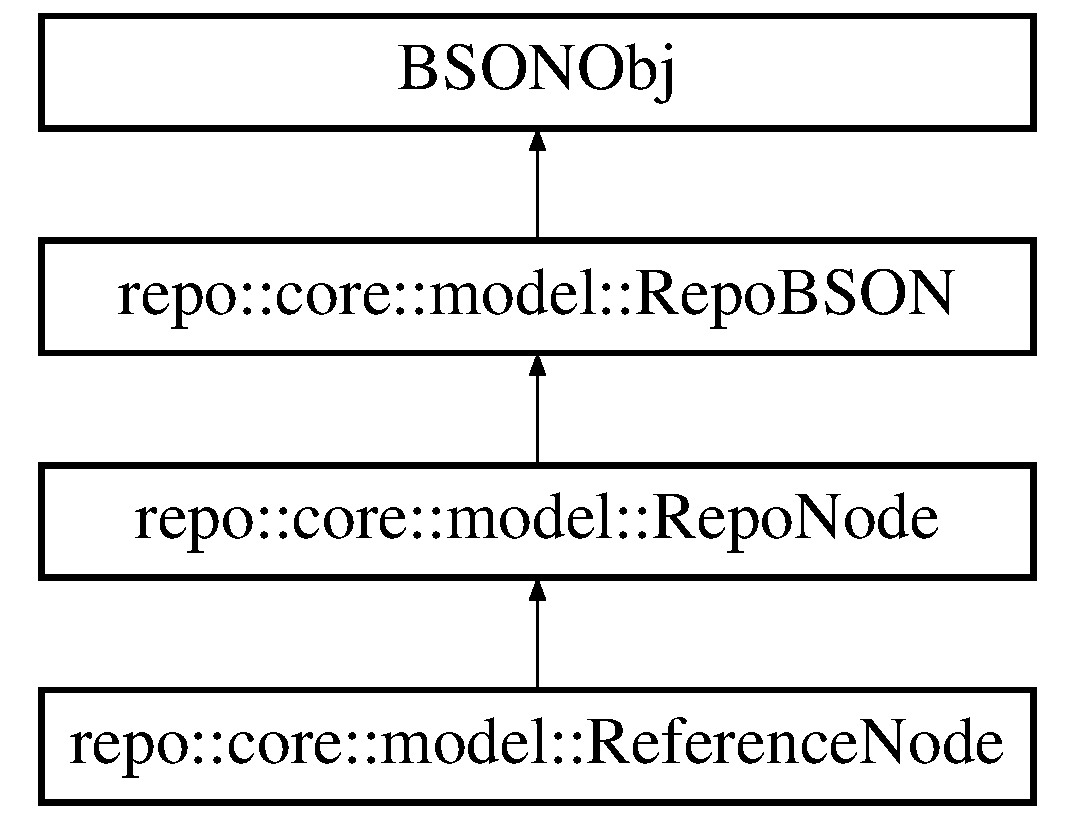
\includegraphics[height=4.000000cm]{classrepo_1_1core_1_1model_1_1_reference_node}
\end{center}
\end{figure}
\subsection*{Public Member Functions}
\begin{DoxyCompactItemize}
\item 
\hyperlink{classrepo_1_1core_1_1model_1_1_reference_node_a36cce27b04a4d55b7c09cb6ab478ce8a}{Reference\+Node} ()
\item 
\hyperlink{classrepo_1_1core_1_1model_1_1_reference_node_a320a317c1892981e028c1d9d04d890f4}{Reference\+Node} (\hyperlink{classrepo_1_1core_1_1model_1_1_repo_b_s_o_n}{Repo\+B\+S\+O\+N} bson)
\item 
\hyperlink{classrepo_1_1core_1_1model_1_1_reference_node_a909cd607b7faa7b319c7c5dfef84cf9d}{$\sim$\+Reference\+Node} ()
\item 
virtual std\+::string \hyperlink{classrepo_1_1core_1_1model_1_1_reference_node_a1f1b1c966eb936b31b92f05247df58d0}{get\+Type} () const 
\item 
virtual Node\+Type \hyperlink{classrepo_1_1core_1_1model_1_1_reference_node_abe69afbcb44f14ad6a9a821819a2cf85}{get\+Type\+As\+Enum} () const 
\item 
virtual bool \hyperlink{classrepo_1_1core_1_1model_1_1_reference_node_abc948b4ed5437871142d57498a12cf2d}{s\+Equal} (const \hyperlink{classrepo_1_1core_1_1model_1_1_repo_node}{Repo\+Node} \&other) const 
\item 
repo\+U\+U\+I\+D \hyperlink{classrepo_1_1core_1_1model_1_1_reference_node_ad3ddd679d4da323c1a8a8ad0aa3077ce}{get\+Revision\+I\+D} () const 
\item 
std\+::string \hyperlink{classrepo_1_1core_1_1model_1_1_reference_node_a2e26797f48595031dc2dbc249cae6e07}{get\+Database\+Name} () const 
\item 
std\+::string \hyperlink{classrepo_1_1core_1_1model_1_1_reference_node_a75be3b6d6b19c190cdfa1bb412cecf4c}{get\+Project\+Name} () const 
\item 
bool \hyperlink{classrepo_1_1core_1_1model_1_1_reference_node_a8b2e959a6af066cb89f0c734e5debe39}{use\+Specific\+Revision} () const 
\end{DoxyCompactItemize}
\subsection*{Additional Inherited Members}


\subsection{Constructor \& Destructor Documentation}
\hypertarget{classrepo_1_1core_1_1model_1_1_reference_node_a36cce27b04a4d55b7c09cb6ab478ce8a}{}\index{repo\+::core\+::model\+::\+Reference\+Node@{repo\+::core\+::model\+::\+Reference\+Node}!Reference\+Node@{Reference\+Node}}
\index{Reference\+Node@{Reference\+Node}!repo\+::core\+::model\+::\+Reference\+Node@{repo\+::core\+::model\+::\+Reference\+Node}}
\subsubsection[{Reference\+Node}]{\setlength{\rightskip}{0pt plus 5cm}Reference\+Node\+::\+Reference\+Node (
\begin{DoxyParamCaption}
{}
\end{DoxyParamCaption}
)}\label{classrepo_1_1core_1_1model_1_1_reference_node_a36cce27b04a4d55b7c09cb6ab478ce8a}
Default constructor \hypertarget{classrepo_1_1core_1_1model_1_1_reference_node_a320a317c1892981e028c1d9d04d890f4}{}\index{repo\+::core\+::model\+::\+Reference\+Node@{repo\+::core\+::model\+::\+Reference\+Node}!Reference\+Node@{Reference\+Node}}
\index{Reference\+Node@{Reference\+Node}!repo\+::core\+::model\+::\+Reference\+Node@{repo\+::core\+::model\+::\+Reference\+Node}}
\subsubsection[{Reference\+Node}]{\setlength{\rightskip}{0pt plus 5cm}Reference\+Node\+::\+Reference\+Node (
\begin{DoxyParamCaption}
\item[{{\bf Repo\+B\+S\+O\+N}}]{bson}
\end{DoxyParamCaption}
)}\label{classrepo_1_1core_1_1model_1_1_reference_node_a320a317c1892981e028c1d9d04d890f4}
Construct a \hyperlink{classrepo_1_1core_1_1model_1_1_reference_node}{Reference\+Node} from a \hyperlink{classrepo_1_1core_1_1model_1_1_repo_b_s_o_n}{Repo\+B\+S\+O\+N} object 
\begin{DoxyParams}{Parameters}
{\em \hyperlink{classrepo_1_1core_1_1model_1_1_repo_b_s_o_n}{Repo\+B\+S\+O\+N}} & object \\
\hline
\end{DoxyParams}
\hypertarget{classrepo_1_1core_1_1model_1_1_reference_node_a909cd607b7faa7b319c7c5dfef84cf9d}{}\index{repo\+::core\+::model\+::\+Reference\+Node@{repo\+::core\+::model\+::\+Reference\+Node}!````~Reference\+Node@{$\sim$\+Reference\+Node}}
\index{````~Reference\+Node@{$\sim$\+Reference\+Node}!repo\+::core\+::model\+::\+Reference\+Node@{repo\+::core\+::model\+::\+Reference\+Node}}
\subsubsection[{$\sim$\+Reference\+Node}]{\setlength{\rightskip}{0pt plus 5cm}Reference\+Node\+::$\sim$\+Reference\+Node (
\begin{DoxyParamCaption}
{}
\end{DoxyParamCaption}
)}\label{classrepo_1_1core_1_1model_1_1_reference_node_a909cd607b7faa7b319c7c5dfef84cf9d}
Default deconstructor 

\subsection{Member Function Documentation}
\hypertarget{classrepo_1_1core_1_1model_1_1_reference_node_a2e26797f48595031dc2dbc249cae6e07}{}\index{repo\+::core\+::model\+::\+Reference\+Node@{repo\+::core\+::model\+::\+Reference\+Node}!get\+Database\+Name@{get\+Database\+Name}}
\index{get\+Database\+Name@{get\+Database\+Name}!repo\+::core\+::model\+::\+Reference\+Node@{repo\+::core\+::model\+::\+Reference\+Node}}
\subsubsection[{get\+Database\+Name}]{\setlength{\rightskip}{0pt plus 5cm}std\+::string repo\+::core\+::model\+::\+Reference\+Node\+::get\+Database\+Name (
\begin{DoxyParamCaption}
{}
\end{DoxyParamCaption}
) const\hspace{0.3cm}{\ttfamily [inline]}}\label{classrepo_1_1core_1_1model_1_1_reference_node_a2e26797f48595031dc2dbc249cae6e07}
Retrieve the project this reference node is referring to \begin{DoxyReturn}{Returns}
returns the project name for this reference 
\end{DoxyReturn}
\hypertarget{classrepo_1_1core_1_1model_1_1_reference_node_a75be3b6d6b19c190cdfa1bb412cecf4c}{}\index{repo\+::core\+::model\+::\+Reference\+Node@{repo\+::core\+::model\+::\+Reference\+Node}!get\+Project\+Name@{get\+Project\+Name}}
\index{get\+Project\+Name@{get\+Project\+Name}!repo\+::core\+::model\+::\+Reference\+Node@{repo\+::core\+::model\+::\+Reference\+Node}}
\subsubsection[{get\+Project\+Name}]{\setlength{\rightskip}{0pt plus 5cm}std\+::string repo\+::core\+::model\+::\+Reference\+Node\+::get\+Project\+Name (
\begin{DoxyParamCaption}
{}
\end{DoxyParamCaption}
) const\hspace{0.3cm}{\ttfamily [inline]}}\label{classrepo_1_1core_1_1model_1_1_reference_node_a75be3b6d6b19c190cdfa1bb412cecf4c}
Retrieve the project this reference node is referring to \begin{DoxyReturn}{Returns}
returns the project name for this reference 
\end{DoxyReturn}
\hypertarget{classrepo_1_1core_1_1model_1_1_reference_node_ad3ddd679d4da323c1a8a8ad0aa3077ce}{}\index{repo\+::core\+::model\+::\+Reference\+Node@{repo\+::core\+::model\+::\+Reference\+Node}!get\+Revision\+I\+D@{get\+Revision\+I\+D}}
\index{get\+Revision\+I\+D@{get\+Revision\+I\+D}!repo\+::core\+::model\+::\+Reference\+Node@{repo\+::core\+::model\+::\+Reference\+Node}}
\subsubsection[{get\+Revision\+I\+D}]{\setlength{\rightskip}{0pt plus 5cm}repo\+U\+U\+I\+D repo\+::core\+::model\+::\+Reference\+Node\+::get\+Revision\+I\+D (
\begin{DoxyParamCaption}
{}
\end{DoxyParamCaption}
) const\hspace{0.3cm}{\ttfamily [inline]}}\label{classrepo_1_1core_1_1model_1_1_reference_node_ad3ddd679d4da323c1a8a8ad0aa3077ce}
Retrieve the U\+U\+I\+D of the revision this reference node is referring to if it doesn\textquotesingle{}t exist, return master branch id \begin{DoxyReturn}{Returns}
returns the U\+U\+I\+D for this reference 
\end{DoxyReturn}
\hypertarget{classrepo_1_1core_1_1model_1_1_reference_node_a1f1b1c966eb936b31b92f05247df58d0}{}\index{repo\+::core\+::model\+::\+Reference\+Node@{repo\+::core\+::model\+::\+Reference\+Node}!get\+Type@{get\+Type}}
\index{get\+Type@{get\+Type}!repo\+::core\+::model\+::\+Reference\+Node@{repo\+::core\+::model\+::\+Reference\+Node}}
\subsubsection[{get\+Type}]{\setlength{\rightskip}{0pt plus 5cm}virtual std\+::string repo\+::core\+::model\+::\+Reference\+Node\+::get\+Type (
\begin{DoxyParamCaption}
{}
\end{DoxyParamCaption}
) const\hspace{0.3cm}{\ttfamily [inline]}, {\ttfamily [virtual]}}\label{classrepo_1_1core_1_1model_1_1_reference_node_a1f1b1c966eb936b31b92f05247df58d0}
Get the type of node \begin{DoxyReturn}{Returns}
returns the type as a string 
\end{DoxyReturn}


Reimplemented from \hyperlink{classrepo_1_1core_1_1model_1_1_repo_node_a4380ba349235b5d9b13b41e41975805e}{repo\+::core\+::model\+::\+Repo\+Node}.

\hypertarget{classrepo_1_1core_1_1model_1_1_reference_node_abe69afbcb44f14ad6a9a821819a2cf85}{}\index{repo\+::core\+::model\+::\+Reference\+Node@{repo\+::core\+::model\+::\+Reference\+Node}!get\+Type\+As\+Enum@{get\+Type\+As\+Enum}}
\index{get\+Type\+As\+Enum@{get\+Type\+As\+Enum}!repo\+::core\+::model\+::\+Reference\+Node@{repo\+::core\+::model\+::\+Reference\+Node}}
\subsubsection[{get\+Type\+As\+Enum}]{\setlength{\rightskip}{0pt plus 5cm}virtual Node\+Type repo\+::core\+::model\+::\+Reference\+Node\+::get\+Type\+As\+Enum (
\begin{DoxyParamCaption}
{}
\end{DoxyParamCaption}
) const\hspace{0.3cm}{\ttfamily [inline]}, {\ttfamily [virtual]}}\label{classrepo_1_1core_1_1model_1_1_reference_node_abe69afbcb44f14ad6a9a821819a2cf85}
Get the type of node as an enum \begin{DoxyReturn}{Returns}
returns type as enum. 
\end{DoxyReturn}


Reimplemented from \hyperlink{classrepo_1_1core_1_1model_1_1_repo_node_ad8d5295248dc9beb0b91efb2ce3b61f4}{repo\+::core\+::model\+::\+Repo\+Node}.

\hypertarget{classrepo_1_1core_1_1model_1_1_reference_node_abc948b4ed5437871142d57498a12cf2d}{}\index{repo\+::core\+::model\+::\+Reference\+Node@{repo\+::core\+::model\+::\+Reference\+Node}!s\+Equal@{s\+Equal}}
\index{s\+Equal@{s\+Equal}!repo\+::core\+::model\+::\+Reference\+Node@{repo\+::core\+::model\+::\+Reference\+Node}}
\subsubsection[{s\+Equal}]{\setlength{\rightskip}{0pt plus 5cm}bool Reference\+Node\+::s\+Equal (
\begin{DoxyParamCaption}
\item[{const {\bf Repo\+Node} \&}]{other}
\end{DoxyParamCaption}
) const\hspace{0.3cm}{\ttfamily [virtual]}}\label{classrepo_1_1core_1_1model_1_1_reference_node_abc948b4ed5437871142d57498a12cf2d}
Check if the node is semantically equal to another Different node should have a different interpretation of what this means. 
\begin{DoxyParams}{Parameters}
{\em other} & node to compare with \\
\hline
{\em returns} & true if equal, false otherwise \\
\hline
\end{DoxyParams}


Reimplemented from \hyperlink{classrepo_1_1core_1_1model_1_1_repo_node_a7c98830a876ee6516587a8f07c7015a5}{repo\+::core\+::model\+::\+Repo\+Node}.

\hypertarget{classrepo_1_1core_1_1model_1_1_reference_node_a8b2e959a6af066cb89f0c734e5debe39}{}\index{repo\+::core\+::model\+::\+Reference\+Node@{repo\+::core\+::model\+::\+Reference\+Node}!use\+Specific\+Revision@{use\+Specific\+Revision}}
\index{use\+Specific\+Revision@{use\+Specific\+Revision}!repo\+::core\+::model\+::\+Reference\+Node@{repo\+::core\+::model\+::\+Reference\+Node}}
\subsubsection[{use\+Specific\+Revision}]{\setlength{\rightskip}{0pt plus 5cm}bool repo\+::core\+::model\+::\+Reference\+Node\+::use\+Specific\+Revision (
\begin{DoxyParamCaption}
{}
\end{DoxyParamCaption}
) const\hspace{0.3cm}{\ttfamily [inline]}}\label{classrepo_1_1core_1_1model_1_1_reference_node_a8b2e959a6af066cb89f0c734e5debe39}
Indicates if the Revision I\+D from \hyperlink{classrepo_1_1core_1_1model_1_1_reference_node_ad3ddd679d4da323c1a8a8ad0aa3077ce}{get\+Revision\+I\+D()} is a branch I\+D (false) or a specific revision(true) \begin{DoxyReturn}{Returns}
returns true if it is a uuid of a specific revision, otherwise it\textquotesingle{}s a branch uuid 
\end{DoxyReturn}


The documentation for this class was generated from the following files\+:\begin{DoxyCompactItemize}
\item 
C\+:/\+Users/\+Carmen/3\+D Repo/\+Repo/3drepobouncer/bouncer/src/repo/core/model/bson/repo\+\_\+node\+\_\+reference.\+h\item 
C\+:/\+Users/\+Carmen/3\+D Repo/\+Repo/3drepobouncer/bouncer/src/repo/core/model/bson/repo\+\_\+node\+\_\+reference.\+cpp\end{DoxyCompactItemize}

\hypertarget{structrepo__color4d__t}{}\section{repo\+\_\+color4d\+\_\+t Struct Reference}
\label{structrepo__color4d__t}\index{repo\+\_\+color4d\+\_\+t@{repo\+\_\+color4d\+\_\+t}}
\subsection*{Public Attributes}
\begin{DoxyCompactItemize}
\item 
\hypertarget{structrepo__color4d__t_a49e81f544a6356ce280f7e8365d17373}{}float {\bfseries r}\label{structrepo__color4d__t_a49e81f544a6356ce280f7e8365d17373}

\item 
\hypertarget{structrepo__color4d__t_adcc911902da587a5b4578ff32e34dc20}{}float {\bfseries g}\label{structrepo__color4d__t_adcc911902da587a5b4578ff32e34dc20}

\item 
\hypertarget{structrepo__color4d__t_a8a53e5ac55404a0e706be135be06d992}{}float {\bfseries b}\label{structrepo__color4d__t_a8a53e5ac55404a0e706be135be06d992}

\item 
\hypertarget{structrepo__color4d__t_aed28c0ac51b30c80377a6e460fa11171}{}float {\bfseries a}\label{structrepo__color4d__t_aed28c0ac51b30c80377a6e460fa11171}

\end{DoxyCompactItemize}


The documentation for this struct was generated from the following file\+:\begin{DoxyCompactItemize}
\item 
C\+:/\+Users/\+Carmen/3\+D Repo/\+Repo/3drepobouncer/bouncer/src/repo/core/model/repo\+\_\+node\+\_\+utils.\+h\end{DoxyCompactItemize}

\hypertarget{structrepo__diff__result__t}{}\section{repo\+\_\+diff\+\_\+result\+\_\+t Struct Reference}
\label{structrepo__diff__result__t}\index{repo\+\_\+diff\+\_\+result\+\_\+t@{repo\+\_\+diff\+\_\+result\+\_\+t}}
\subsection*{Public Attributes}
\begin{DoxyCompactItemize}
\item 
\hypertarget{structrepo__diff__result__t_af3d8fe09b919ccd0cfcfdc2c3d0ca6ef}{}std\+::vector$<$ repo\+U\+U\+I\+D $>$ {\bfseries added}\label{structrepo__diff__result__t_af3d8fe09b919ccd0cfcfdc2c3d0ca6ef}

\item 
\hypertarget{structrepo__diff__result__t_a810771908512970e98f6365e0b21664a}{}std\+::vector$<$ repo\+U\+U\+I\+D $>$ {\bfseries modified}\label{structrepo__diff__result__t_a810771908512970e98f6365e0b21664a}

\item 
\hypertarget{structrepo__diff__result__t_a07f698d79eb68be682fece9f7edef8c5}{}std\+::unordered\+\_\+map$<$ repo\+U\+U\+I\+D, repo\+U\+U\+I\+D, \hyperlink{struct_repo_u_u_i_d_hasher}{Repo\+U\+U\+I\+D\+Hasher} $>$ {\bfseries correspondence}\label{structrepo__diff__result__t_a07f698d79eb68be682fece9f7edef8c5}

\end{DoxyCompactItemize}


The documentation for this struct was generated from the following file\+:\begin{DoxyCompactItemize}
\item 
C\+:/\+Users/\+Carmen/3\+D Repo/\+Repo/3drepobouncer/bouncer/src/repo/lib/datastructure/repo\+\_\+structs.\+h\end{DoxyCompactItemize}

\hypertarget{structrepo__material__t}{}\section{repo\+\_\+material\+\_\+t Struct Reference}
\label{structrepo__material__t}\index{repo\+\_\+material\+\_\+t@{repo\+\_\+material\+\_\+t}}
\subsection*{Public Attributes}
\begin{DoxyCompactItemize}
\item 
\hypertarget{structrepo__material__t_acc39d617cb31b9f8417a53e464946733}{}std\+::vector$<$ float $>$ {\bfseries ambient}\label{structrepo__material__t_acc39d617cb31b9f8417a53e464946733}

\item 
\hypertarget{structrepo__material__t_ad9b46adb8b69f65d077f95877fb56b17}{}std\+::vector$<$ float $>$ {\bfseries diffuse}\label{structrepo__material__t_ad9b46adb8b69f65d077f95877fb56b17}

\item 
\hypertarget{structrepo__material__t_a2412943dd92702fdcd4d836cf0b91f79}{}std\+::vector$<$ float $>$ {\bfseries specular}\label{structrepo__material__t_a2412943dd92702fdcd4d836cf0b91f79}

\item 
\hypertarget{structrepo__material__t_ae25a423c04f1222cc5c5251dfbedab59}{}std\+::vector$<$ float $>$ {\bfseries emissive}\label{structrepo__material__t_ae25a423c04f1222cc5c5251dfbedab59}

\item 
\hypertarget{structrepo__material__t_a5ddee39ae30e46d7df9ab92164a70e78}{}float {\bfseries opacity}\label{structrepo__material__t_a5ddee39ae30e46d7df9ab92164a70e78}

\item 
\hypertarget{structrepo__material__t_a58128a39e5d8834c1ff4285be45f9d02}{}float {\bfseries shininess}\label{structrepo__material__t_a58128a39e5d8834c1ff4285be45f9d02}

\item 
\hypertarget{structrepo__material__t_af43b3c2118c59f3f21e620d74910664b}{}float {\bfseries shininess\+Strength}\label{structrepo__material__t_af43b3c2118c59f3f21e620d74910664b}

\item 
\hypertarget{structrepo__material__t_a4b6b0aba0c04a5cf3528f9c133133c61}{}bool {\bfseries is\+Wireframe}\label{structrepo__material__t_a4b6b0aba0c04a5cf3528f9c133133c61}

\item 
\hypertarget{structrepo__material__t_ac6341815992c22777814997f7d7278e5}{}bool {\bfseries is\+Two\+Sided}\label{structrepo__material__t_ac6341815992c22777814997f7d7278e5}

\end{DoxyCompactItemize}


The documentation for this struct was generated from the following file\+:\begin{DoxyCompactItemize}
\item 
C\+:/\+Users/\+Carmen/3\+D Repo/\+Repo/3drepobouncer/bouncer/src/repo/core/model/repo\+\_\+node\+\_\+utils.\+h\end{DoxyCompactItemize}

\hypertarget{structrepo__mesh__entry__t}{}\section{repo\+\_\+mesh\+\_\+entry\+\_\+t Struct Reference}
\label{structrepo__mesh__entry__t}\index{repo\+\_\+mesh\+\_\+entry\+\_\+t@{repo\+\_\+mesh\+\_\+entry\+\_\+t}}
\subsection*{Public Attributes}
\begin{DoxyCompactItemize}
\item 
\hypertarget{structrepo__mesh__entry__t_ad457b26fd9e1063c67256dd4850a1e0a}{}std\+::vector$<$ float $>$ {\bfseries min}\label{structrepo__mesh__entry__t_ad457b26fd9e1063c67256dd4850a1e0a}

\item 
\hypertarget{structrepo__mesh__entry__t_ab955d0154a8f9b54f83482abbf27b8aa}{}std\+::vector$<$ float $>$ {\bfseries max}\label{structrepo__mesh__entry__t_ab955d0154a8f9b54f83482abbf27b8aa}

\item 
\hypertarget{structrepo__mesh__entry__t_ae3f1b9322d26f8a6a3a9923b9946da2b}{}std\+::vector$<$ float $>$ {\bfseries mid}\label{structrepo__mesh__entry__t_ae3f1b9322d26f8a6a3a9923b9946da2b}

\item 
\hypertarget{structrepo__mesh__entry__t_a506ae567e99926f08b8df79f37f5e8d0}{}repo\+U\+U\+I\+D {\bfseries id}\label{structrepo__mesh__entry__t_a506ae567e99926f08b8df79f37f5e8d0}

\end{DoxyCompactItemize}


The documentation for this struct was generated from the following file\+:\begin{DoxyCompactItemize}
\item 
C\+:/\+Users/\+Carmen/3\+D Repo/\+Repo/3drepobouncer/bouncer/src/repo/lib/datastructure/repo\+\_\+structs.\+h\end{DoxyCompactItemize}

\hypertarget{structrepo__mesh__mapping__t}{}\section{repo\+\_\+mesh\+\_\+mapping\+\_\+t Struct Reference}
\label{structrepo__mesh__mapping__t}\index{repo\+\_\+mesh\+\_\+mapping\+\_\+t@{repo\+\_\+mesh\+\_\+mapping\+\_\+t}}
\subsection*{Public Attributes}
\begin{DoxyCompactItemize}
\item 
\hypertarget{structrepo__mesh__mapping__t_a64c13a942cb509903088fe5f3255bba9}{}\hyperlink{structrepo__vector__t}{repo\+\_\+vector\+\_\+t} {\bfseries min}\label{structrepo__mesh__mapping__t_a64c13a942cb509903088fe5f3255bba9}

\item 
\hypertarget{structrepo__mesh__mapping__t_a5dd76d8702119d7e1cbc635578381bb8}{}\hyperlink{structrepo__vector__t}{repo\+\_\+vector\+\_\+t} {\bfseries max}\label{structrepo__mesh__mapping__t_a5dd76d8702119d7e1cbc635578381bb8}

\item 
\hypertarget{structrepo__mesh__mapping__t_a3a91bd07456a32a1777a8bc7f493912d}{}repo\+U\+U\+I\+D {\bfseries mesh\+\_\+id}\label{structrepo__mesh__mapping__t_a3a91bd07456a32a1777a8bc7f493912d}

\item 
\hypertarget{structrepo__mesh__mapping__t_affa918b8fd09578de7044f51fe1812bc}{}repo\+U\+U\+I\+D {\bfseries material\+\_\+id}\label{structrepo__mesh__mapping__t_affa918b8fd09578de7044f51fe1812bc}

\item 
\hypertarget{structrepo__mesh__mapping__t_abe6446a1ba73e81296bf1be3dfcb27fd}{}int32\+\_\+t {\bfseries vert\+From}\label{structrepo__mesh__mapping__t_abe6446a1ba73e81296bf1be3dfcb27fd}

\item 
\hypertarget{structrepo__mesh__mapping__t_ac0adbd9a7d900cf83cb2406c47ea9291}{}int32\+\_\+t {\bfseries vert\+To}\label{structrepo__mesh__mapping__t_ac0adbd9a7d900cf83cb2406c47ea9291}

\item 
\hypertarget{structrepo__mesh__mapping__t_a878d2ef1b43afb1deaa0e8130bf5bc81}{}int32\+\_\+t {\bfseries tri\+From}\label{structrepo__mesh__mapping__t_a878d2ef1b43afb1deaa0e8130bf5bc81}

\item 
\hypertarget{structrepo__mesh__mapping__t_ab5dc942ac42234ba663c45da65f1f361}{}int32\+\_\+t {\bfseries tri\+To}\label{structrepo__mesh__mapping__t_ab5dc942ac42234ba663c45da65f1f361}

\end{DoxyCompactItemize}


The documentation for this struct was generated from the following file\+:\begin{DoxyCompactItemize}
\item 
C\+:/\+Users/\+Carmen/3\+D Repo/\+Repo/3drepobouncer/bouncer/src/repo/core/model/repo\+\_\+node\+\_\+utils.\+h\end{DoxyCompactItemize}

\hypertarget{structrepo__partitioning__tree__t}{}\section{repo\+\_\+partitioning\+\_\+tree\+\_\+t Struct Reference}
\label{structrepo__partitioning__tree__t}\index{repo\+\_\+partitioning\+\_\+tree\+\_\+t@{repo\+\_\+partitioning\+\_\+tree\+\_\+t}}
\subsection*{Public Member Functions}
\begin{DoxyCompactItemize}
\item 
\hypertarget{structrepo__partitioning__tree__t_a461f9d14df2bc25f3330a610dd255caf}{}{\bfseries repo\+\_\+partitioning\+\_\+tree\+\_\+t} (const repo\+::\+Partitioning\+Tree\+Type \&type, const float \&p\+Value, std\+::shared\+\_\+ptr$<$ \hyperlink{structrepo__partitioning__tree__t}{repo\+\_\+partitioning\+\_\+tree\+\_\+t} $>$ left, std\+::shared\+\_\+ptr$<$ \hyperlink{structrepo__partitioning__tree__t}{repo\+\_\+partitioning\+\_\+tree\+\_\+t} $>$ right)\label{structrepo__partitioning__tree__t_a461f9d14df2bc25f3330a610dd255caf}

\item 
\hypertarget{structrepo__partitioning__tree__t_a38423dbc2457f935d31cf748b52dce2c}{}{\bfseries repo\+\_\+partitioning\+\_\+tree\+\_\+t} (const std\+::vector$<$ \hyperlink{structrepo__mesh__entry__t}{repo\+\_\+mesh\+\_\+entry\+\_\+t} $>$ \&meshes)\label{structrepo__partitioning__tree__t_a38423dbc2457f935d31cf748b52dce2c}

\end{DoxyCompactItemize}
\subsection*{Public Attributes}
\begin{DoxyCompactItemize}
\item 
\hypertarget{structrepo__partitioning__tree__t_a50608492dd6a19de604e49791b1ce205}{}repo\+::\+Partitioning\+Tree\+Type {\bfseries type}\label{structrepo__partitioning__tree__t_a50608492dd6a19de604e49791b1ce205}

\item 
\hypertarget{structrepo__partitioning__tree__t_a2297db3056b0c3f86af98eb7fd03b553}{}std\+::vector$<$ \hyperlink{structrepo__mesh__entry__t}{repo\+\_\+mesh\+\_\+entry\+\_\+t} $>$ {\bfseries meshes}\label{structrepo__partitioning__tree__t_a2297db3056b0c3f86af98eb7fd03b553}

\item 
\hypertarget{structrepo__partitioning__tree__t_ae528381e051e7845e018601206f1fb84}{}float {\bfseries p\+Value}\label{structrepo__partitioning__tree__t_ae528381e051e7845e018601206f1fb84}

\item 
\hypertarget{structrepo__partitioning__tree__t_aeefc3aa701a5dc08fb95cfeedc19c2e3}{}std\+::shared\+\_\+ptr$<$ \hyperlink{structrepo__partitioning__tree__t}{repo\+\_\+partitioning\+\_\+tree\+\_\+t} $>$ {\bfseries left}\label{structrepo__partitioning__tree__t_aeefc3aa701a5dc08fb95cfeedc19c2e3}

\item 
\hypertarget{structrepo__partitioning__tree__t_a2d619be91780ace2a48b98b0bc22d390}{}std\+::shared\+\_\+ptr$<$ \hyperlink{structrepo__partitioning__tree__t}{repo\+\_\+partitioning\+\_\+tree\+\_\+t} $>$ {\bfseries right}\label{structrepo__partitioning__tree__t_a2d619be91780ace2a48b98b0bc22d390}

\end{DoxyCompactItemize}


The documentation for this struct was generated from the following file\+:\begin{DoxyCompactItemize}
\item 
C\+:/\+Users/\+Carmen/3\+D Repo/\+Repo/3drepobouncer/bouncer/src/repo/lib/datastructure/repo\+\_\+structs.\+h\end{DoxyCompactItemize}

\hypertarget{structrepo__vector2d__t}{}\section{repo\+\_\+vector2d\+\_\+t Struct Reference}
\label{structrepo__vector2d__t}\index{repo\+\_\+vector2d\+\_\+t@{repo\+\_\+vector2d\+\_\+t}}
\subsection*{Public Attributes}
\begin{DoxyCompactItemize}
\item 
\hypertarget{structrepo__vector2d__t_ad23a694bf6472563ca75baa3879c40be}{}float {\bfseries x}\label{structrepo__vector2d__t_ad23a694bf6472563ca75baa3879c40be}

\item 
\hypertarget{structrepo__vector2d__t_ace5a8377be4c8a9a69e731861df01a8f}{}float {\bfseries y}\label{structrepo__vector2d__t_ace5a8377be4c8a9a69e731861df01a8f}

\end{DoxyCompactItemize}


The documentation for this struct was generated from the following file\+:\begin{DoxyCompactItemize}
\item 
C\+:/\+Users/\+Carmen/3\+D Repo/\+Repo/3drepobouncer/bouncer/src/repo/core/model/repo\+\_\+node\+\_\+utils.\+h\end{DoxyCompactItemize}

\hypertarget{structrepo__vector__t}{}\section{repo\+\_\+vector\+\_\+t Struct Reference}
\label{structrepo__vector__t}\index{repo\+\_\+vector\+\_\+t@{repo\+\_\+vector\+\_\+t}}
\subsection*{Public Attributes}
\begin{DoxyCompactItemize}
\item 
\hypertarget{structrepo__vector__t_aedc4d3bd4a28c15f8cff00d37cd9db98}{}float {\bfseries x}\label{structrepo__vector__t_aedc4d3bd4a28c15f8cff00d37cd9db98}

\item 
\hypertarget{structrepo__vector__t_a18d3391aa6f971cb125bbab9a4c6fc4c}{}float {\bfseries y}\label{structrepo__vector__t_a18d3391aa6f971cb125bbab9a4c6fc4c}

\item 
\hypertarget{structrepo__vector__t_a6bec151d27475aeaa3ead41e4c614779}{}float {\bfseries z}\label{structrepo__vector__t_a6bec151d27475aeaa3ead41e4c614779}

\end{DoxyCompactItemize}


The documentation for this struct was generated from the following file\+:\begin{DoxyCompactItemize}
\item 
C\+:/\+Users/\+Carmen/3\+D Repo/\+Repo/3drepobouncer/bouncer/src/repo/core/model/repo\+\_\+node\+\_\+utils.\+h\end{DoxyCompactItemize}

\hypertarget{structrepo__web__buffers__t}{}\section{repo\+\_\+web\+\_\+buffers\+\_\+t Struct Reference}
\label{structrepo__web__buffers__t}\index{repo\+\_\+web\+\_\+buffers\+\_\+t@{repo\+\_\+web\+\_\+buffers\+\_\+t}}


{\ttfamily \#include $<$repo\+\_\+structs.\+h$>$}

\subsection*{Public Attributes}
\begin{DoxyCompactItemize}
\item 
\hypertarget{structrepo__web__buffers__t_a906b00c40edb2a3970b287508d2ac595}{}std\+::unordered\+\_\+map$<$ std\+::string, std\+::vector$<$ uint8\+\_\+t $>$ $>$ {\bfseries geo\+Files}\label{structrepo__web__buffers__t_a906b00c40edb2a3970b287508d2ac595}

\item 
\hypertarget{structrepo__web__buffers__t_af22fbdf81f61f19f59edf60c39aaca02}{}std\+::unordered\+\_\+map$<$ std\+::string, std\+::vector$<$ uint8\+\_\+t $>$ $>$ {\bfseries x3d\+Files}\label{structrepo__web__buffers__t_af22fbdf81f61f19f59edf60c39aaca02}

\item 
\hypertarget{structrepo__web__buffers__t_abefcc3f739928fa1ce1eadd88f6e7e01}{}std\+::unordered\+\_\+map$<$ std\+::string, std\+::vector$<$ uint8\+\_\+t $>$ $>$ {\bfseries json\+Files}\label{structrepo__web__buffers__t_abefcc3f739928fa1ce1eadd88f6e7e01}

\end{DoxyCompactItemize}


\subsection{Detailed Description}
Copyright (C) 2016 3\+D Repo Ltd

This program is free software\+: you can redistribute it and/or modify it under the terms of the G\+N\+U Affero General Public License as published by the Free Software Foundation, either version 3 of the License, or (at your option) any later version.

This program is distributed in the hope that it will be useful, but W\+I\+T\+H\+O\+U\+T A\+N\+Y W\+A\+R\+R\+A\+N\+T\+Y; without even the implied warranty of M\+E\+R\+C\+H\+A\+N\+T\+A\+B\+I\+L\+I\+T\+Y or F\+I\+T\+N\+E\+S\+S F\+O\+R A P\+A\+R\+T\+I\+C\+U\+L\+A\+R P\+U\+R\+P\+O\+S\+E. See the G\+N\+U Affero General Public License for more details.

You should have received a copy of the G\+N\+U Affero General Public License along with this program. If not, see \href{http://www.gnu.org/licenses/}{\tt http\+://www.\+gnu.\+org/licenses/}. 

The documentation for this struct was generated from the following file\+:\begin{DoxyCompactItemize}
\item 
C\+:/\+Users/\+Carmen/3\+D Repo/\+Repo/3drepobouncer/bouncer/src/repo/lib/datastructure/repo\+\_\+structs.\+h\end{DoxyCompactItemize}

\hypertarget{classrepo_1_1lib_1_1_repo_abstract_listener}{}\section{repo\+:\+:lib\+:\+:Repo\+Abstract\+Listener Class Reference}
\label{classrepo_1_1lib_1_1_repo_abstract_listener}\index{repo\+::lib\+::\+Repo\+Abstract\+Listener@{repo\+::lib\+::\+Repo\+Abstract\+Listener}}
Inheritance diagram for repo\+:\+:lib\+:\+:Repo\+Abstract\+Listener\+:\begin{figure}[H]
\begin{center}
\leavevmode
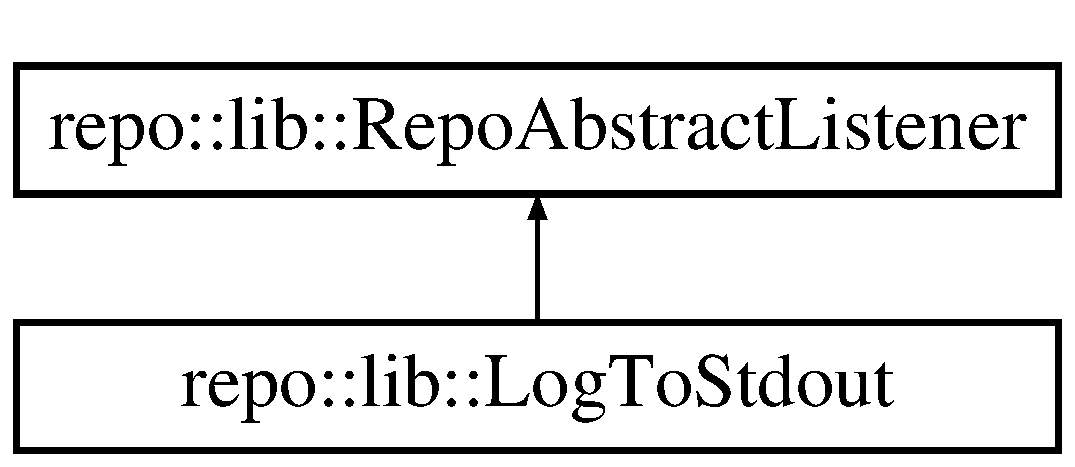
\includegraphics[height=2.000000cm]{classrepo_1_1lib_1_1_repo_abstract_listener}
\end{center}
\end{figure}
\subsection*{Public Member Functions}
\begin{DoxyCompactItemize}
\item 
\hypertarget{classrepo_1_1lib_1_1_repo_abstract_listener_a7b3b335339d33c19c0152021a2ab60b5}{}virtual void {\bfseries message\+Generated} (const std\+::string \&message)=0\label{classrepo_1_1lib_1_1_repo_abstract_listener_a7b3b335339d33c19c0152021a2ab60b5}

\end{DoxyCompactItemize}


The documentation for this class was generated from the following file\+:\begin{DoxyCompactItemize}
\item 
C\+:/\+Users/\+Carmen/3\+D Repo/\+Repo/3drepobouncer/bouncer/src/repo/lib/repo\+\_\+listener\+\_\+abstract.\+h\end{DoxyCompactItemize}

\hypertarget{classrepo_1_1lib_1_1_repo_broadcaster}{}\section{repo\+:\+:lib\+:\+:Repo\+Broadcaster Class Reference}
\label{classrepo_1_1lib_1_1_repo_broadcaster}\index{repo\+::lib\+::\+Repo\+Broadcaster@{repo\+::lib\+::\+Repo\+Broadcaster}}
Inheritance diagram for repo\+:\+:lib\+:\+:Repo\+Broadcaster\+:\begin{figure}[H]
\begin{center}
\leavevmode
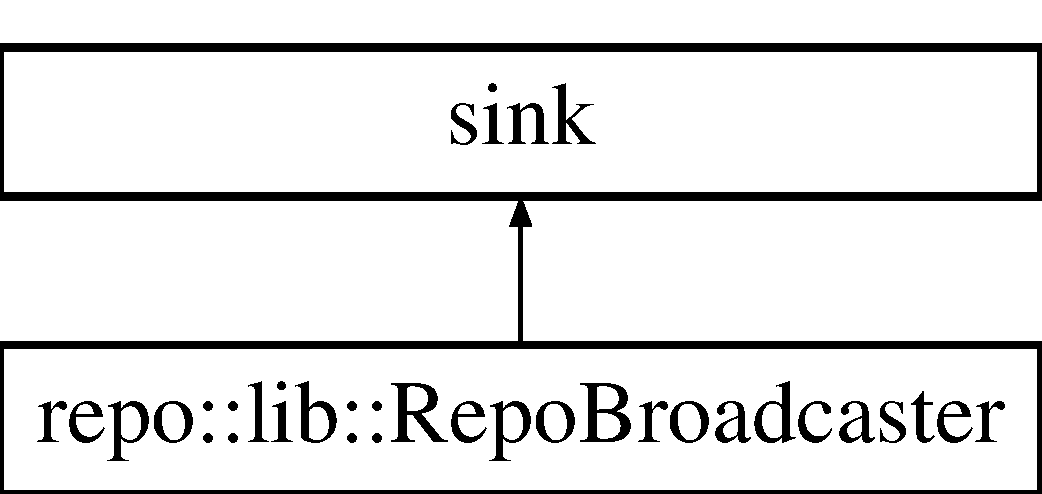
\includegraphics[height=2.000000cm]{classrepo_1_1lib_1_1_repo_broadcaster}
\end{center}
\end{figure}
\subsection*{Public Member Functions}
\begin{DoxyCompactItemize}
\item 
\hyperlink{classrepo_1_1lib_1_1_repo_broadcaster_aee1e729b0da691e2ce0de046a5b2bc8d}{Repo\+Broadcaster} ()
\item 
void \hyperlink{classrepo_1_1lib_1_1_repo_broadcaster_ad369dbbcd5cf62a71840a361119b9308}{subscribe} (\hyperlink{classrepo_1_1lib_1_1_repo_abstract_listener}{Repo\+Abstract\+Listener} $\ast$subscriber)
\item 
std\+::streamsize \hyperlink{classrepo_1_1lib_1_1_repo_broadcaster_a655a000a33c1f471de202b35ea3d4623}{write} (const char $\ast$s, std\+::streamsize n)
\end{DoxyCompactItemize}


\subsection{Constructor \& Destructor Documentation}
\hypertarget{classrepo_1_1lib_1_1_repo_broadcaster_aee1e729b0da691e2ce0de046a5b2bc8d}{}\index{repo\+::lib\+::\+Repo\+Broadcaster@{repo\+::lib\+::\+Repo\+Broadcaster}!Repo\+Broadcaster@{Repo\+Broadcaster}}
\index{Repo\+Broadcaster@{Repo\+Broadcaster}!repo\+::lib\+::\+Repo\+Broadcaster@{repo\+::lib\+::\+Repo\+Broadcaster}}
\subsubsection[{Repo\+Broadcaster}]{\setlength{\rightskip}{0pt plus 5cm}Repo\+Broadcaster\+::\+Repo\+Broadcaster (
\begin{DoxyParamCaption}
{}
\end{DoxyParamCaption}
)}\label{classrepo_1_1lib_1_1_repo_broadcaster_aee1e729b0da691e2ce0de046a5b2bc8d}
F\+I\+X\+M\+E\+: should be a private constructor -\/ singleton class. 

\subsection{Member Function Documentation}
\hypertarget{classrepo_1_1lib_1_1_repo_broadcaster_ad369dbbcd5cf62a71840a361119b9308}{}\index{repo\+::lib\+::\+Repo\+Broadcaster@{repo\+::lib\+::\+Repo\+Broadcaster}!subscribe@{subscribe}}
\index{subscribe@{subscribe}!repo\+::lib\+::\+Repo\+Broadcaster@{repo\+::lib\+::\+Repo\+Broadcaster}}
\subsubsection[{subscribe}]{\setlength{\rightskip}{0pt plus 5cm}void repo\+::lib\+::\+Repo\+Broadcaster\+::subscribe (
\begin{DoxyParamCaption}
\item[{{\bf Repo\+Abstract\+Listener} $\ast$}]{subscriber}
\end{DoxyParamCaption}
)\hspace{0.3cm}{\ttfamily [inline]}}\label{classrepo_1_1lib_1_1_repo_broadcaster_ad369dbbcd5cf62a71840a361119b9308}
Subscribe to the broadcaster 
\begin{DoxyParams}{Parameters}
{\em subscriber} & An object to notify when there are new messages \\
\hline
\end{DoxyParams}
\hypertarget{classrepo_1_1lib_1_1_repo_broadcaster_a655a000a33c1f471de202b35ea3d4623}{}\index{repo\+::lib\+::\+Repo\+Broadcaster@{repo\+::lib\+::\+Repo\+Broadcaster}!write@{write}}
\index{write@{write}!repo\+::lib\+::\+Repo\+Broadcaster@{repo\+::lib\+::\+Repo\+Broadcaster}}
\subsubsection[{write}]{\setlength{\rightskip}{0pt plus 5cm}std\+::streamsize Repo\+Broadcaster\+::write (
\begin{DoxyParamCaption}
\item[{const char $\ast$}]{s, }
\item[{std\+::streamsize}]{n}
\end{DoxyParamCaption}
)}\label{classrepo_1_1lib_1_1_repo_broadcaster_a655a000a33c1f471de202b35ea3d4623}
When called, it will notify all subscribers of the message. 

The documentation for this class was generated from the following files\+:\begin{DoxyCompactItemize}
\item 
C\+:/\+Users/\+Carmen/3\+D Repo/\+Repo/3drepobouncer/bouncer/src/repo/lib/repo\+\_\+broadcaster.\+h\item 
C\+:/\+Users/\+Carmen/3\+D Repo/\+Repo/3drepobouncer/bouncer/src/repo/lib/repo\+\_\+broadcaster.\+cpp\end{DoxyCompactItemize}

\hypertarget{classrepo_1_1core_1_1model_1_1_repo_b_s_o_n}{}\section{repo\+:\+:core\+:\+:model\+:\+:Repo\+B\+S\+O\+N Class Reference}
\label{classrepo_1_1core_1_1model_1_1_repo_b_s_o_n}\index{repo\+::core\+::model\+::\+Repo\+B\+S\+O\+N@{repo\+::core\+::model\+::\+Repo\+B\+S\+O\+N}}
Inheritance diagram for repo\+:\+:core\+:\+:model\+:\+:Repo\+B\+S\+O\+N\+:\begin{figure}[H]
\begin{center}
\leavevmode
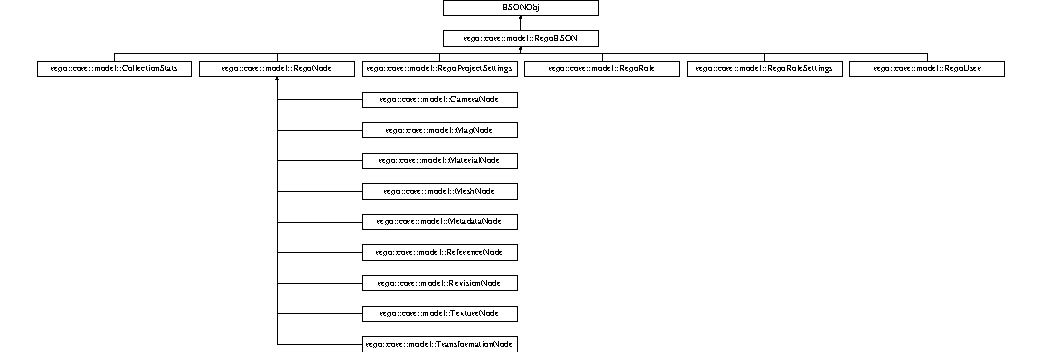
\includegraphics[height=4.725739cm]{classrepo_1_1core_1_1model_1_1_repo_b_s_o_n}
\end{center}
\end{figure}
\subsection*{Public Member Functions}
\begin{DoxyCompactItemize}
\item 
\hyperlink{classrepo_1_1core_1_1model_1_1_repo_b_s_o_n_a354d143bf35f8bc6c4224835f6ba9ca5}{Repo\+B\+S\+O\+N} ()
\item 
\hyperlink{classrepo_1_1core_1_1model_1_1_repo_b_s_o_n_aabc885b5853e080d67b40f1a5e246844}{Repo\+B\+S\+O\+N} (const mongo\+::\+B\+S\+O\+N\+Obj \&obj, const std\+::unordered\+\_\+map$<$ std\+::string, std\+::pair$<$ std\+::string, std\+::vector$<$ uint8\+\_\+t $>$$>$$>$ \&bin\+Mapping=std\+::unordered\+\_\+map$<$ std\+::string, std\+::pair$<$ std\+::string, std\+::vector$<$ uint8\+\_\+t $>$$>$$>$())
\item 
\hyperlink{classrepo_1_1core_1_1model_1_1_repo_b_s_o_n_aa06f776e2e40cfdc2987b862830ac0d9}{Repo\+B\+S\+O\+N} (mongo\+::\+B\+S\+O\+N\+Obj\+Builder \&builder)
\item 
\hyperlink{classrepo_1_1core_1_1model_1_1_repo_b_s_o_n_a24345f6cbb37297891d438137392d14a}{Repo\+B\+S\+O\+N} (const std\+::vector$<$ char $>$ \&raw\+Data)
\item 
virtual \hyperlink{classrepo_1_1core_1_1model_1_1_repo_b_s_o_n_a67460b346bf65fab93b57fdaf8b3048c}{$\sim$\+Repo\+B\+S\+O\+N} ()
\item 
\hyperlink{classrepo_1_1core_1_1model_1_1_repo_b_s_o_n}{Repo\+B\+S\+O\+N} \& \hyperlink{classrepo_1_1core_1_1model_1_1_repo_b_s_o_n_a57637989afe6afdad35530365d8881c4}{operator=} (\hyperlink{classrepo_1_1core_1_1model_1_1_repo_b_s_o_n}{Repo\+B\+S\+O\+N} other\+Copy)
\item 
void \hyperlink{classrepo_1_1core_1_1model_1_1_repo_b_s_o_n_a55fbe89c9c724ea6f2413c60d7510afc}{swap} (\hyperlink{classrepo_1_1core_1_1model_1_1_repo_b_s_o_n}{Repo\+B\+S\+O\+N} other\+Copy)
\item 
\hyperlink{classrepo_1_1core_1_1model_1_1_repo_b_s_o_n_element}{Repo\+B\+S\+O\+N\+Element} \hyperlink{classrepo_1_1core_1_1model_1_1_repo_b_s_o_n_aa2352078eb863b969d3a858166e22803}{get\+Field} (const std\+::string \&label) const 
\item 
{\footnotesize template$<$class T $>$ }\\bool \hyperlink{classrepo_1_1core_1_1model_1_1_repo_b_s_o_n_a6264631f8009beb55f7402f486fd63f8}{get\+Binary\+Field\+As\+Vector} (const std\+::string \&field, std\+::vector$<$ T $>$ \&vec) const 
\item 
repo\+U\+U\+I\+D \hyperlink{classrepo_1_1core_1_1model_1_1_repo_b_s_o_n_abc38f95304405ad3c5f988473fb6e62d}{get\+U\+U\+I\+D\+Field} (const std\+::string \&label) const 
\item 
std\+::vector$<$ repo\+U\+U\+I\+D $>$ \hyperlink{classrepo_1_1core_1_1model_1_1_repo_b_s_o_n_ac42db2ae14159fb1e625bfe7d5578733}{get\+U\+U\+I\+D\+Field\+Array} (const std\+::string \&label) const 
\item 
std\+::vector$<$ float $>$ \hyperlink{classrepo_1_1core_1_1model_1_1_repo_b_s_o_n_aef8f7857b6d4a317d128b627d41a6c7c}{get\+Float\+Array} (const std\+::string \&label) const 
\item 
std\+::vector$<$ std\+::string $>$ \hyperlink{classrepo_1_1core_1_1model_1_1_repo_b_s_o_n_a1f6ee4d979027c5ccd521a8cc90291e5}{get\+String\+Array} (const std\+::string \&label) const 
\item 
int64\+\_\+t \hyperlink{classrepo_1_1core_1_1model_1_1_repo_b_s_o_n_afebb889f385500484149529f93d05179}{get\+Time\+Stamp\+Field} (const std\+::string \&label) const 
\item 
std\+::list$<$ std\+::pair$<$ std\+::string, std\+::string $>$ $>$ \hyperlink{classrepo_1_1core_1_1model_1_1_repo_b_s_o_n_ab4568b7a3f53275af3c0925a8b822137}{get\+List\+String\+Pair\+Field} (const std\+::string \&arr\+Label, const std\+::string \&fst\+Label, const std\+::string \&snd\+Label) const 
\item 
\hypertarget{classrepo_1_1core_1_1model_1_1_repo_b_s_o_n_a0a7279d5d7e3c09a8276e26d18ef4ba4}{}double \hyperlink{classrepo_1_1core_1_1model_1_1_repo_b_s_o_n_a0a7279d5d7e3c09a8276e26d18ef4ba4}{get\+Embedded\+Double} (const std\+::string \&embedded\+Obj\+Name, const std\+::string \&field\+Name, const double \&default\+Value=0) const \label{classrepo_1_1core_1_1model_1_1_repo_b_s_o_n_a0a7279d5d7e3c09a8276e26d18ef4ba4}

\begin{DoxyCompactList}\small\item\em Gets double from embedded sub-\/object based on name fields. \end{DoxyCompactList}\item 
\hypertarget{classrepo_1_1core_1_1model_1_1_repo_b_s_o_n_a3e49b65ed21750fb260f100ed640bec4}{}bool \hyperlink{classrepo_1_1core_1_1model_1_1_repo_b_s_o_n_a3e49b65ed21750fb260f100ed640bec4}{has\+Embedded\+Field} (const std\+::string \&embedded\+Obj\+Name, const std\+::string \&field\+Name) const \label{classrepo_1_1core_1_1model_1_1_repo_b_s_o_n_a3e49b65ed21750fb260f100ed640bec4}

\begin{DoxyCompactList}\small\item\em Returns true if embedded object contains given field\+Name. \end{DoxyCompactList}\item 
bool \hyperlink{classrepo_1_1core_1_1model_1_1_repo_b_s_o_n_a0ad5a02a94a02313e22bd8826c1db8cc}{has\+Bin\+Field} (const std\+::string \&label) const 
\item 
\hypertarget{classrepo_1_1core_1_1model_1_1_repo_b_s_o_n_a08eb34b8ed7ecb5546e6f99e4708c3be}{}virtual \hyperlink{classrepo_1_1core_1_1model_1_1_repo_b_s_o_n}{Repo\+B\+S\+O\+N} {\bfseries clone\+And\+Add\+Fields} (const \hyperlink{classrepo_1_1core_1_1model_1_1_repo_b_s_o_n}{Repo\+B\+S\+O\+N} $\ast$changes) const \label{classrepo_1_1core_1_1model_1_1_repo_b_s_o_n_a08eb34b8ed7ecb5546e6f99e4708c3be}

\item 
\hyperlink{classrepo_1_1core_1_1model_1_1_repo_b_s_o_n}{Repo\+B\+S\+O\+N} \hyperlink{classrepo_1_1core_1_1model_1_1_repo_b_s_o_n_ac4825e1c7c40c46fc9f5b1ba2ff1e8bf}{clone\+And\+Shrink} () const 
\item 
\hypertarget{classrepo_1_1core_1_1model_1_1_repo_b_s_o_n_ab47dba25bea609596e1201d65163df80}{}std\+::vector$<$ uint8\+\_\+t $>$ {\bfseries get\+Big\+Binary} (const std\+::string \&key) const \label{classrepo_1_1core_1_1model_1_1_repo_b_s_o_n_ab47dba25bea609596e1201d65163df80}

\item 
std\+::vector$<$ std\+::pair$<$ std\+::string, std\+::string $>$ $>$ \hyperlink{classrepo_1_1core_1_1model_1_1_repo_b_s_o_n_af6fcb689bfd5fb93e43a3e6879332fbb}{get\+File\+List} () const 
\item 
std\+::unordered\+\_\+map$<$ std\+::string, std\+::pair$<$ std\+::string, std\+::vector$<$ uint8\+\_\+t $>$ $>$ $>$ \hyperlink{classrepo_1_1core_1_1model_1_1_repo_b_s_o_n_ae61dbbcf6f836bffda5f5bb6cd596145}{get\+Files\+Mapping} () const 
\item 
bool \hyperlink{classrepo_1_1core_1_1model_1_1_repo_b_s_o_n_a75e57c9424a02f7e71ff755bc06d933b}{has\+Oversize\+Files} () const 
\end{DoxyCompactItemize}
\subsection*{Static Public Member Functions}
\begin{DoxyCompactItemize}
\item 
static \hyperlink{classrepo_1_1core_1_1model_1_1_repo_b_s_o_n}{Repo\+B\+S\+O\+N} \hyperlink{classrepo_1_1core_1_1model_1_1_repo_b_s_o_n_ab46a47cac46bc975bf6fde6702ba0f7d}{from\+J\+S\+O\+N} (const std\+::string \&json)
\item 
static int64\+\_\+t \hyperlink{classrepo_1_1core_1_1model_1_1_repo_b_s_o_n_a2c7f83c92e6a293162ccc6814bf0aa9c}{get\+Current\+Timestamp} ()
\end{DoxyCompactItemize}
\subsection*{Protected Attributes}
\begin{DoxyCompactItemize}
\item 
\hypertarget{classrepo_1_1core_1_1model_1_1_repo_b_s_o_n_a8c8cbce2af3478baec967ec854ac4ff0}{}std\+::unordered\+\_\+map$<$ std\+::string, std\+::pair$<$ std\+::string, std\+::vector$<$ uint8\+\_\+t $>$ $>$ $>$ {\bfseries big\+Files}\label{classrepo_1_1core_1_1model_1_1_repo_b_s_o_n_a8c8cbce2af3478baec967ec854ac4ff0}

\end{DoxyCompactItemize}


\subsection{Constructor \& Destructor Documentation}
\hypertarget{classrepo_1_1core_1_1model_1_1_repo_b_s_o_n_a354d143bf35f8bc6c4224835f6ba9ca5}{}\index{repo\+::core\+::model\+::\+Repo\+B\+S\+O\+N@{repo\+::core\+::model\+::\+Repo\+B\+S\+O\+N}!Repo\+B\+S\+O\+N@{Repo\+B\+S\+O\+N}}
\index{Repo\+B\+S\+O\+N@{Repo\+B\+S\+O\+N}!repo\+::core\+::model\+::\+Repo\+B\+S\+O\+N@{repo\+::core\+::model\+::\+Repo\+B\+S\+O\+N}}
\subsubsection[{Repo\+B\+S\+O\+N}]{\setlength{\rightskip}{0pt plus 5cm}repo\+::core\+::model\+::\+Repo\+B\+S\+O\+N\+::\+Repo\+B\+S\+O\+N (
\begin{DoxyParamCaption}
{}
\end{DoxyParamCaption}
)\hspace{0.3cm}{\ttfamily [inline]}}\label{classrepo_1_1core_1_1model_1_1_repo_b_s_o_n_a354d143bf35f8bc6c4224835f6ba9ca5}
Default empty constructor. \hypertarget{classrepo_1_1core_1_1model_1_1_repo_b_s_o_n_aabc885b5853e080d67b40f1a5e246844}{}\index{repo\+::core\+::model\+::\+Repo\+B\+S\+O\+N@{repo\+::core\+::model\+::\+Repo\+B\+S\+O\+N}!Repo\+B\+S\+O\+N@{Repo\+B\+S\+O\+N}}
\index{Repo\+B\+S\+O\+N@{Repo\+B\+S\+O\+N}!repo\+::core\+::model\+::\+Repo\+B\+S\+O\+N@{repo\+::core\+::model\+::\+Repo\+B\+S\+O\+N}}
\subsubsection[{Repo\+B\+S\+O\+N}]{\setlength{\rightskip}{0pt plus 5cm}Repo\+B\+S\+O\+N\+::\+Repo\+B\+S\+O\+N (
\begin{DoxyParamCaption}
\item[{const mongo\+::\+B\+S\+O\+N\+Obj \&}]{obj, }
\item[{const std\+::unordered\+\_\+map$<$ std\+::string, std\+::pair$<$ std\+::string, std\+::vector$<$ uint8\+\_\+t $>$$>$$>$ \&}]{bin\+Mapping = {\ttfamily std\+:\+:unordered\+\_\+map$<$std\+:\+:string,~std\+:\+:pair$<$std\+:\+:string,~std\+:\+:vector$<$uint8\+\_\+t$>$$>$$>$()}}
\end{DoxyParamCaption}
)}\label{classrepo_1_1core_1_1model_1_1_repo_b_s_o_n_aabc885b5853e080d67b40f1a5e246844}
Constructor from Mongo B\+S\+O\+N object. 
\begin{DoxyParams}{Parameters}
{\em mongo} & B\+S\+O\+N object \\
\hline
\end{DoxyParams}
\hypertarget{classrepo_1_1core_1_1model_1_1_repo_b_s_o_n_aa06f776e2e40cfdc2987b862830ac0d9}{}\index{repo\+::core\+::model\+::\+Repo\+B\+S\+O\+N@{repo\+::core\+::model\+::\+Repo\+B\+S\+O\+N}!Repo\+B\+S\+O\+N@{Repo\+B\+S\+O\+N}}
\index{Repo\+B\+S\+O\+N@{Repo\+B\+S\+O\+N}!repo\+::core\+::model\+::\+Repo\+B\+S\+O\+N@{repo\+::core\+::model\+::\+Repo\+B\+S\+O\+N}}
\subsubsection[{Repo\+B\+S\+O\+N}]{\setlength{\rightskip}{0pt plus 5cm}repo\+::core\+::model\+::\+Repo\+B\+S\+O\+N\+::\+Repo\+B\+S\+O\+N (
\begin{DoxyParamCaption}
\item[{mongo\+::\+B\+S\+O\+N\+Obj\+Builder \&}]{builder}
\end{DoxyParamCaption}
)\hspace{0.3cm}{\ttfamily [inline]}}\label{classrepo_1_1core_1_1model_1_1_repo_b_s_o_n_aa06f776e2e40cfdc2987b862830ac0d9}
Constructor from Mongo B\+S\+O\+N object builder. 
\begin{DoxyParams}{Parameters}
{\em mongo} & B\+S\+O\+N object builder \\
\hline
\end{DoxyParams}
\hypertarget{classrepo_1_1core_1_1model_1_1_repo_b_s_o_n_a24345f6cbb37297891d438137392d14a}{}\index{repo\+::core\+::model\+::\+Repo\+B\+S\+O\+N@{repo\+::core\+::model\+::\+Repo\+B\+S\+O\+N}!Repo\+B\+S\+O\+N@{Repo\+B\+S\+O\+N}}
\index{Repo\+B\+S\+O\+N@{Repo\+B\+S\+O\+N}!repo\+::core\+::model\+::\+Repo\+B\+S\+O\+N@{repo\+::core\+::model\+::\+Repo\+B\+S\+O\+N}}
\subsubsection[{Repo\+B\+S\+O\+N}]{\setlength{\rightskip}{0pt plus 5cm}repo\+::core\+::model\+::\+Repo\+B\+S\+O\+N\+::\+Repo\+B\+S\+O\+N (
\begin{DoxyParamCaption}
\item[{const std\+::vector$<$ char $>$ \&}]{raw\+Data}
\end{DoxyParamCaption}
)\hspace{0.3cm}{\ttfamily [inline]}}\label{classrepo_1_1core_1_1model_1_1_repo_b_s_o_n_a24345f6cbb37297891d438137392d14a}
Constructor from raw data buffer. 
\begin{DoxyParams}{Parameters}
{\em raw\+Data} & raw data \\
\hline
\end{DoxyParams}
\hypertarget{classrepo_1_1core_1_1model_1_1_repo_b_s_o_n_a67460b346bf65fab93b57fdaf8b3048c}{}\index{repo\+::core\+::model\+::\+Repo\+B\+S\+O\+N@{repo\+::core\+::model\+::\+Repo\+B\+S\+O\+N}!````~Repo\+B\+S\+O\+N@{$\sim$\+Repo\+B\+S\+O\+N}}
\index{````~Repo\+B\+S\+O\+N@{$\sim$\+Repo\+B\+S\+O\+N}!repo\+::core\+::model\+::\+Repo\+B\+S\+O\+N@{repo\+::core\+::model\+::\+Repo\+B\+S\+O\+N}}
\subsubsection[{$\sim$\+Repo\+B\+S\+O\+N}]{\setlength{\rightskip}{0pt plus 5cm}virtual repo\+::core\+::model\+::\+Repo\+B\+S\+O\+N\+::$\sim$\+Repo\+B\+S\+O\+N (
\begin{DoxyParamCaption}
{}
\end{DoxyParamCaption}
)\hspace{0.3cm}{\ttfamily [inline]}, {\ttfamily [virtual]}}\label{classrepo_1_1core_1_1model_1_1_repo_b_s_o_n_a67460b346bf65fab93b57fdaf8b3048c}
Default empty deconstructor. 

\subsection{Member Function Documentation}
\hypertarget{classrepo_1_1core_1_1model_1_1_repo_b_s_o_n_ac4825e1c7c40c46fc9f5b1ba2ff1e8bf}{}\index{repo\+::core\+::model\+::\+Repo\+B\+S\+O\+N@{repo\+::core\+::model\+::\+Repo\+B\+S\+O\+N}!clone\+And\+Shrink@{clone\+And\+Shrink}}
\index{clone\+And\+Shrink@{clone\+And\+Shrink}!repo\+::core\+::model\+::\+Repo\+B\+S\+O\+N@{repo\+::core\+::model\+::\+Repo\+B\+S\+O\+N}}
\subsubsection[{clone\+And\+Shrink}]{\setlength{\rightskip}{0pt plus 5cm}{\bf Repo\+B\+S\+O\+N} Repo\+B\+S\+O\+N\+::clone\+And\+Shrink (
\begin{DoxyParamCaption}
{}
\end{DoxyParamCaption}
) const}\label{classrepo_1_1core_1_1model_1_1_repo_b_s_o_n_ac4825e1c7c40c46fc9f5b1ba2ff1e8bf}
Clone and attempt the shrink the bson by offloading binary files to big file storage \begin{DoxyReturn}{Returns}
returns the shrunk B\+S\+O\+N 
\end{DoxyReturn}
\hypertarget{classrepo_1_1core_1_1model_1_1_repo_b_s_o_n_ab46a47cac46bc975bf6fde6702ba0f7d}{}\index{repo\+::core\+::model\+::\+Repo\+B\+S\+O\+N@{repo\+::core\+::model\+::\+Repo\+B\+S\+O\+N}!from\+J\+S\+O\+N@{from\+J\+S\+O\+N}}
\index{from\+J\+S\+O\+N@{from\+J\+S\+O\+N}!repo\+::core\+::model\+::\+Repo\+B\+S\+O\+N@{repo\+::core\+::model\+::\+Repo\+B\+S\+O\+N}}
\subsubsection[{from\+J\+S\+O\+N}]{\setlength{\rightskip}{0pt plus 5cm}{\bf Repo\+B\+S\+O\+N} Repo\+B\+S\+O\+N\+::from\+J\+S\+O\+N (
\begin{DoxyParamCaption}
\item[{const std\+::string \&}]{json}
\end{DoxyParamCaption}
)\hspace{0.3cm}{\ttfamily [static]}}\label{classrepo_1_1core_1_1model_1_1_repo_b_s_o_n_ab46a47cac46bc975bf6fde6702ba0f7d}
Construct a repobson from a json string \hypertarget{classrepo_1_1core_1_1model_1_1_repo_b_s_o_n_a6264631f8009beb55f7402f486fd63f8}{}\index{repo\+::core\+::model\+::\+Repo\+B\+S\+O\+N@{repo\+::core\+::model\+::\+Repo\+B\+S\+O\+N}!get\+Binary\+Field\+As\+Vector@{get\+Binary\+Field\+As\+Vector}}
\index{get\+Binary\+Field\+As\+Vector@{get\+Binary\+Field\+As\+Vector}!repo\+::core\+::model\+::\+Repo\+B\+S\+O\+N@{repo\+::core\+::model\+::\+Repo\+B\+S\+O\+N}}
\subsubsection[{get\+Binary\+Field\+As\+Vector}]{\setlength{\rightskip}{0pt plus 5cm}template$<$class T $>$ bool repo\+::core\+::model\+::\+Repo\+B\+S\+O\+N\+::get\+Binary\+Field\+As\+Vector (
\begin{DoxyParamCaption}
\item[{const std\+::string \&}]{field, }
\item[{std\+::vector$<$ T $>$ \&}]{vec}
\end{DoxyParamCaption}
) const\hspace{0.3cm}{\ttfamily [inline]}}\label{classrepo_1_1core_1_1model_1_1_repo_b_s_o_n_a6264631f8009beb55f7402f486fd63f8}
get a binary field in the form of vector of T 
\begin{DoxyParams}{Parameters}
{\em field} & field name \\
\hline
{\em vec} & pointer to a vector to store this data \\
\hline
\end{DoxyParams}
\begin{DoxyReturn}{Returns}
returns true upon success. 
\end{DoxyReturn}
\hypertarget{classrepo_1_1core_1_1model_1_1_repo_b_s_o_n_a2c7f83c92e6a293162ccc6814bf0aa9c}{}\index{repo\+::core\+::model\+::\+Repo\+B\+S\+O\+N@{repo\+::core\+::model\+::\+Repo\+B\+S\+O\+N}!get\+Current\+Timestamp@{get\+Current\+Timestamp}}
\index{get\+Current\+Timestamp@{get\+Current\+Timestamp}!repo\+::core\+::model\+::\+Repo\+B\+S\+O\+N@{repo\+::core\+::model\+::\+Repo\+B\+S\+O\+N}}
\subsubsection[{get\+Current\+Timestamp}]{\setlength{\rightskip}{0pt plus 5cm}int64\+\_\+t Repo\+B\+S\+O\+N\+::get\+Current\+Timestamp (
\begin{DoxyParamCaption}
{}
\end{DoxyParamCaption}
)\hspace{0.3cm}{\ttfamily [static]}}\label{classrepo_1_1core_1_1model_1_1_repo_b_s_o_n_a2c7f83c92e6a293162ccc6814bf0aa9c}
Returns the current time in the form of int64 timestamp \hypertarget{classrepo_1_1core_1_1model_1_1_repo_b_s_o_n_aa2352078eb863b969d3a858166e22803}{}\index{repo\+::core\+::model\+::\+Repo\+B\+S\+O\+N@{repo\+::core\+::model\+::\+Repo\+B\+S\+O\+N}!get\+Field@{get\+Field}}
\index{get\+Field@{get\+Field}!repo\+::core\+::model\+::\+Repo\+B\+S\+O\+N@{repo\+::core\+::model\+::\+Repo\+B\+S\+O\+N}}
\subsubsection[{get\+Field}]{\setlength{\rightskip}{0pt plus 5cm}{\bf Repo\+B\+S\+O\+N\+Element} repo\+::core\+::model\+::\+Repo\+B\+S\+O\+N\+::get\+Field (
\begin{DoxyParamCaption}
\item[{const std\+::string \&}]{label}
\end{DoxyParamCaption}
) const\hspace{0.3cm}{\ttfamily [inline]}}\label{classrepo_1_1core_1_1model_1_1_repo_b_s_o_n_aa2352078eb863b969d3a858166e22803}
returns a field from the B\+S\+O\+N 
\begin{DoxyParams}{Parameters}
{\em label} & name of the field to retrieve \\
\hline
\end{DoxyParams}
\begin{DoxyReturn}{Returns}
returns a \hyperlink{classrepo_1_1core_1_1model_1_1_repo_b_s_o_n_element}{Repo\+B\+S\+O\+N\+Element} 
\end{DoxyReturn}
\hypertarget{classrepo_1_1core_1_1model_1_1_repo_b_s_o_n_af6fcb689bfd5fb93e43a3e6879332fbb}{}\index{repo\+::core\+::model\+::\+Repo\+B\+S\+O\+N@{repo\+::core\+::model\+::\+Repo\+B\+S\+O\+N}!get\+File\+List@{get\+File\+List}}
\index{get\+File\+List@{get\+File\+List}!repo\+::core\+::model\+::\+Repo\+B\+S\+O\+N@{repo\+::core\+::model\+::\+Repo\+B\+S\+O\+N}}
\subsubsection[{get\+File\+List}]{\setlength{\rightskip}{0pt plus 5cm}std\+::vector$<$ std\+::pair$<$ std\+::string, std\+::string $>$ $>$ Repo\+B\+S\+O\+N\+::get\+File\+List (
\begin{DoxyParamCaption}
{}
\end{DoxyParamCaption}
) const}\label{classrepo_1_1core_1_1model_1_1_repo_b_s_o_n_af6fcb689bfd5fb93e43a3e6879332fbb}
Get the list of file names for the big files needs to be stored for this bson \begin{DoxyReturn}{Returns}
returns a list of \{field name, file name\} needed to be stored 
\end{DoxyReturn}
\hypertarget{classrepo_1_1core_1_1model_1_1_repo_b_s_o_n_ae61dbbcf6f836bffda5f5bb6cd596145}{}\index{repo\+::core\+::model\+::\+Repo\+B\+S\+O\+N@{repo\+::core\+::model\+::\+Repo\+B\+S\+O\+N}!get\+Files\+Mapping@{get\+Files\+Mapping}}
\index{get\+Files\+Mapping@{get\+Files\+Mapping}!repo\+::core\+::model\+::\+Repo\+B\+S\+O\+N@{repo\+::core\+::model\+::\+Repo\+B\+S\+O\+N}}
\subsubsection[{get\+Files\+Mapping}]{\setlength{\rightskip}{0pt plus 5cm}std\+::unordered\+\_\+map$<$ std\+::string, std\+::pair$<$std\+::string, std\+::vector$<$uint8\+\_\+t$>$ $>$ $>$ repo\+::core\+::model\+::\+Repo\+B\+S\+O\+N\+::get\+Files\+Mapping (
\begin{DoxyParamCaption}
{}
\end{DoxyParamCaption}
) const\hspace{0.3cm}{\ttfamily [inline]}}\label{classrepo_1_1core_1_1model_1_1_repo_b_s_o_n_ae61dbbcf6f836bffda5f5bb6cd596145}
Get the mapping files from the bson object \begin{DoxyReturn}{Returns}
returns the map of external (grid\+F\+S) files 
\end{DoxyReturn}
\hypertarget{classrepo_1_1core_1_1model_1_1_repo_b_s_o_n_aef8f7857b6d4a317d128b627d41a6c7c}{}\index{repo\+::core\+::model\+::\+Repo\+B\+S\+O\+N@{repo\+::core\+::model\+::\+Repo\+B\+S\+O\+N}!get\+Float\+Array@{get\+Float\+Array}}
\index{get\+Float\+Array@{get\+Float\+Array}!repo\+::core\+::model\+::\+Repo\+B\+S\+O\+N@{repo\+::core\+::model\+::\+Repo\+B\+S\+O\+N}}
\subsubsection[{get\+Float\+Array}]{\setlength{\rightskip}{0pt plus 5cm}std\+::vector$<$ float $>$ Repo\+B\+S\+O\+N\+::get\+Float\+Array (
\begin{DoxyParamCaption}
\item[{const std\+::string \&}]{label}
\end{DoxyParamCaption}
) const}\label{classrepo_1_1core_1_1model_1_1_repo_b_s_o_n_aef8f7857b6d4a317d128b627d41a6c7c}
Get an array of fields given an element label 
\begin{DoxyParams}{Parameters}
{\em label} & name of the array element \\
\hline
\end{DoxyParams}
\begin{DoxyReturn}{Returns}
returns the array element in their respective type 
\end{DoxyReturn}
\hypertarget{classrepo_1_1core_1_1model_1_1_repo_b_s_o_n_ab4568b7a3f53275af3c0925a8b822137}{}\index{repo\+::core\+::model\+::\+Repo\+B\+S\+O\+N@{repo\+::core\+::model\+::\+Repo\+B\+S\+O\+N}!get\+List\+String\+Pair\+Field@{get\+List\+String\+Pair\+Field}}
\index{get\+List\+String\+Pair\+Field@{get\+List\+String\+Pair\+Field}!repo\+::core\+::model\+::\+Repo\+B\+S\+O\+N@{repo\+::core\+::model\+::\+Repo\+B\+S\+O\+N}}
\subsubsection[{get\+List\+String\+Pair\+Field}]{\setlength{\rightskip}{0pt plus 5cm}std\+::list$<$ std\+::pair$<$ std\+::string, std\+::string $>$ $>$ Repo\+B\+S\+O\+N\+::get\+List\+String\+Pair\+Field (
\begin{DoxyParamCaption}
\item[{const std\+::string \&}]{arr\+Label, }
\item[{const std\+::string \&}]{fst\+Label, }
\item[{const std\+::string \&}]{snd\+Label}
\end{DoxyParamCaption}
) const}\label{classrepo_1_1core_1_1model_1_1_repo_b_s_o_n_ab4568b7a3f53275af3c0925a8b822137}
Get a field as a List of string pairs This is for scenarios were there is an element that is an array of objects and you want to get 2 fields within all the objects. 
\begin{DoxyParams}{Parameters}
{\em arr\+Label} & the element where this data is stored \\
\hline
{\em fst\+Label} & label for \#1 in pair \\
\hline
{\em snd\+Label} & label for \#2 in pair \\
\hline
\end{DoxyParams}
\begin{DoxyReturn}{Returns}
a List of pairs of strings 
\end{DoxyReturn}
\hypertarget{classrepo_1_1core_1_1model_1_1_repo_b_s_o_n_a1f6ee4d979027c5ccd521a8cc90291e5}{}\index{repo\+::core\+::model\+::\+Repo\+B\+S\+O\+N@{repo\+::core\+::model\+::\+Repo\+B\+S\+O\+N}!get\+String\+Array@{get\+String\+Array}}
\index{get\+String\+Array@{get\+String\+Array}!repo\+::core\+::model\+::\+Repo\+B\+S\+O\+N@{repo\+::core\+::model\+::\+Repo\+B\+S\+O\+N}}
\subsubsection[{get\+String\+Array}]{\setlength{\rightskip}{0pt plus 5cm}std\+::vector$<$ std\+::string $>$ Repo\+B\+S\+O\+N\+::get\+String\+Array (
\begin{DoxyParamCaption}
\item[{const std\+::string \&}]{label}
\end{DoxyParamCaption}
) const}\label{classrepo_1_1core_1_1model_1_1_repo_b_s_o_n_a1f6ee4d979027c5ccd521a8cc90291e5}
Get an array of fields given an element label 
\begin{DoxyParams}{Parameters}
{\em label} & name of the array element \\
\hline
\end{DoxyParams}
\begin{DoxyReturn}{Returns}
returns the array element in their respective type 
\end{DoxyReturn}
\hypertarget{classrepo_1_1core_1_1model_1_1_repo_b_s_o_n_afebb889f385500484149529f93d05179}{}\index{repo\+::core\+::model\+::\+Repo\+B\+S\+O\+N@{repo\+::core\+::model\+::\+Repo\+B\+S\+O\+N}!get\+Time\+Stamp\+Field@{get\+Time\+Stamp\+Field}}
\index{get\+Time\+Stamp\+Field@{get\+Time\+Stamp\+Field}!repo\+::core\+::model\+::\+Repo\+B\+S\+O\+N@{repo\+::core\+::model\+::\+Repo\+B\+S\+O\+N}}
\subsubsection[{get\+Time\+Stamp\+Field}]{\setlength{\rightskip}{0pt plus 5cm}int64\+\_\+t Repo\+B\+S\+O\+N\+::get\+Time\+Stamp\+Field (
\begin{DoxyParamCaption}
\item[{const std\+::string \&}]{label}
\end{DoxyParamCaption}
) const}\label{classrepo_1_1core_1_1model_1_1_repo_b_s_o_n_afebb889f385500484149529f93d05179}
Get a field as timestamp 
\begin{DoxyParams}{Parameters}
{\em label} & name of the element \\
\hline
\end{DoxyParams}
\begin{DoxyReturn}{Returns}
returns timestamp as int64, return -\/1 if not found 
\end{DoxyReturn}
\hypertarget{classrepo_1_1core_1_1model_1_1_repo_b_s_o_n_abc38f95304405ad3c5f988473fb6e62d}{}\index{repo\+::core\+::model\+::\+Repo\+B\+S\+O\+N@{repo\+::core\+::model\+::\+Repo\+B\+S\+O\+N}!get\+U\+U\+I\+D\+Field@{get\+U\+U\+I\+D\+Field}}
\index{get\+U\+U\+I\+D\+Field@{get\+U\+U\+I\+D\+Field}!repo\+::core\+::model\+::\+Repo\+B\+S\+O\+N@{repo\+::core\+::model\+::\+Repo\+B\+S\+O\+N}}
\subsubsection[{get\+U\+U\+I\+D\+Field}]{\setlength{\rightskip}{0pt plus 5cm}repo\+U\+U\+I\+D Repo\+B\+S\+O\+N\+::get\+U\+U\+I\+D\+Field (
\begin{DoxyParamCaption}
\item[{const std\+::string \&}]{label}
\end{DoxyParamCaption}
) const}\label{classrepo_1_1core_1_1model_1_1_repo_b_s_o_n_abc38f95304405ad3c5f988473fb6e62d}
Overload of get\+Field function to retreve repo\+U\+U\+I\+D 
\begin{DoxyParams}{Parameters}
{\em label} & name of the field \\
\hline
\end{DoxyParams}
\begin{DoxyReturn}{Returns}
returns a repo\+U\+U\+I\+D from that field 
\end{DoxyReturn}
\hypertarget{classrepo_1_1core_1_1model_1_1_repo_b_s_o_n_ac42db2ae14159fb1e625bfe7d5578733}{}\index{repo\+::core\+::model\+::\+Repo\+B\+S\+O\+N@{repo\+::core\+::model\+::\+Repo\+B\+S\+O\+N}!get\+U\+U\+I\+D\+Field\+Array@{get\+U\+U\+I\+D\+Field\+Array}}
\index{get\+U\+U\+I\+D\+Field\+Array@{get\+U\+U\+I\+D\+Field\+Array}!repo\+::core\+::model\+::\+Repo\+B\+S\+O\+N@{repo\+::core\+::model\+::\+Repo\+B\+S\+O\+N}}
\subsubsection[{get\+U\+U\+I\+D\+Field\+Array}]{\setlength{\rightskip}{0pt plus 5cm}std\+::vector$<$ repo\+U\+U\+I\+D $>$ Repo\+B\+S\+O\+N\+::get\+U\+U\+I\+D\+Field\+Array (
\begin{DoxyParamCaption}
\item[{const std\+::string \&}]{label}
\end{DoxyParamCaption}
) const}\label{classrepo_1_1core_1_1model_1_1_repo_b_s_o_n_ac42db2ae14159fb1e625bfe7d5578733}
Get an array of fields given an array element 
\begin{DoxyParams}{Parameters}
{\em label} & name of the array element \\
\hline
\end{DoxyParams}
\begin{DoxyReturn}{Returns}
returns the array element in their respective type 
\end{DoxyReturn}
\hypertarget{classrepo_1_1core_1_1model_1_1_repo_b_s_o_n_a0ad5a02a94a02313e22bd8826c1db8cc}{}\index{repo\+::core\+::model\+::\+Repo\+B\+S\+O\+N@{repo\+::core\+::model\+::\+Repo\+B\+S\+O\+N}!has\+Bin\+Field@{has\+Bin\+Field}}
\index{has\+Bin\+Field@{has\+Bin\+Field}!repo\+::core\+::model\+::\+Repo\+B\+S\+O\+N@{repo\+::core\+::model\+::\+Repo\+B\+S\+O\+N}}
\subsubsection[{has\+Bin\+Field}]{\setlength{\rightskip}{0pt plus 5cm}bool repo\+::core\+::model\+::\+Repo\+B\+S\+O\+N\+::has\+Bin\+Field (
\begin{DoxyParamCaption}
\item[{const std\+::string \&}]{label}
\end{DoxyParamCaption}
) const\hspace{0.3cm}{\ttfamily [inline]}}\label{classrepo_1_1core_1_1model_1_1_repo_b_s_o_n_a0ad5a02a94a02313e22bd8826c1db8cc}
Checks if a binary field exists within the \hyperlink{classrepo_1_1core_1_1model_1_1_repo_b_s_o_n}{Repo\+B\+S\+O\+N} This differs from has\+Field() as it also checks the big\+Files mapping where the field is stored outside in Grid\+F\+S. 
\begin{DoxyParams}{Parameters}
{\em label} & field name in question \\
\hline
\end{DoxyParams}
\begin{DoxyReturn}{Returns}
returns true if found 
\end{DoxyReturn}
\hypertarget{classrepo_1_1core_1_1model_1_1_repo_b_s_o_n_a75e57c9424a02f7e71ff755bc06d933b}{}\index{repo\+::core\+::model\+::\+Repo\+B\+S\+O\+N@{repo\+::core\+::model\+::\+Repo\+B\+S\+O\+N}!has\+Oversize\+Files@{has\+Oversize\+Files}}
\index{has\+Oversize\+Files@{has\+Oversize\+Files}!repo\+::core\+::model\+::\+Repo\+B\+S\+O\+N@{repo\+::core\+::model\+::\+Repo\+B\+S\+O\+N}}
\subsubsection[{has\+Oversize\+Files}]{\setlength{\rightskip}{0pt plus 5cm}bool repo\+::core\+::model\+::\+Repo\+B\+S\+O\+N\+::has\+Oversize\+Files (
\begin{DoxyParamCaption}
{}
\end{DoxyParamCaption}
) const\hspace{0.3cm}{\ttfamily [inline]}}\label{classrepo_1_1core_1_1model_1_1_repo_b_s_o_n_a75e57c9424a02f7e71ff755bc06d933b}
Check if this bson object has oversized files \begin{DoxyReturn}{Returns}
returns true if there are oversized files 
\end{DoxyReturn}
\hypertarget{classrepo_1_1core_1_1model_1_1_repo_b_s_o_n_a57637989afe6afdad35530365d8881c4}{}\index{repo\+::core\+::model\+::\+Repo\+B\+S\+O\+N@{repo\+::core\+::model\+::\+Repo\+B\+S\+O\+N}!operator=@{operator=}}
\index{operator=@{operator=}!repo\+::core\+::model\+::\+Repo\+B\+S\+O\+N@{repo\+::core\+::model\+::\+Repo\+B\+S\+O\+N}}
\subsubsection[{operator=}]{\setlength{\rightskip}{0pt plus 5cm}{\bf Repo\+B\+S\+O\+N}\& repo\+::core\+::model\+::\+Repo\+B\+S\+O\+N\+::operator= (
\begin{DoxyParamCaption}
\item[{{\bf Repo\+B\+S\+O\+N}}]{other\+Copy}
\end{DoxyParamCaption}
)\hspace{0.3cm}{\ttfamily [inline]}}\label{classrepo_1_1core_1_1model_1_1_repo_b_s_o_n_a57637989afe6afdad35530365d8881c4}
Override the equals operator to perform the swap just like mongo bson but also retrieve the mapping information \hypertarget{classrepo_1_1core_1_1model_1_1_repo_b_s_o_n_a55fbe89c9c724ea6f2413c60d7510afc}{}\index{repo\+::core\+::model\+::\+Repo\+B\+S\+O\+N@{repo\+::core\+::model\+::\+Repo\+B\+S\+O\+N}!swap@{swap}}
\index{swap@{swap}!repo\+::core\+::model\+::\+Repo\+B\+S\+O\+N@{repo\+::core\+::model\+::\+Repo\+B\+S\+O\+N}}
\subsubsection[{swap}]{\setlength{\rightskip}{0pt plus 5cm}void repo\+::core\+::model\+::\+Repo\+B\+S\+O\+N\+::swap (
\begin{DoxyParamCaption}
\item[{{\bf Repo\+B\+S\+O\+N}}]{other\+Copy}
\end{DoxyParamCaption}
)\hspace{0.3cm}{\ttfamily [inline]}}\label{classrepo_1_1core_1_1model_1_1_repo_b_s_o_n_a55fbe89c9c724ea6f2413c60d7510afc}
Override the swap operator to perform the swap just like mongo bson but also carry over the mapping information 

The documentation for this class was generated from the following files\+:\begin{DoxyCompactItemize}
\item 
C\+:/\+Users/\+Carmen/3\+D Repo/\+Repo/3drepobouncer/bouncer/src/repo/core/model/bson/repo\+\_\+bson.\+h\item 
C\+:/\+Users/\+Carmen/3\+D Repo/\+Repo/3drepobouncer/bouncer/src/repo/core/model/bson/repo\+\_\+bson.\+cpp\end{DoxyCompactItemize}

\hypertarget{classrepo_1_1core_1_1model_1_1_repo_b_s_o_n_builder}{}\section{repo\+:\+:core\+:\+:model\+:\+:Repo\+B\+S\+O\+N\+Builder Class Reference}
\label{classrepo_1_1core_1_1model_1_1_repo_b_s_o_n_builder}\index{repo\+::core\+::model\+::\+Repo\+B\+S\+O\+N\+Builder@{repo\+::core\+::model\+::\+Repo\+B\+S\+O\+N\+Builder}}
Inheritance diagram for repo\+:\+:core\+:\+:model\+:\+:Repo\+B\+S\+O\+N\+Builder\+:\begin{figure}[H]
\begin{center}
\leavevmode
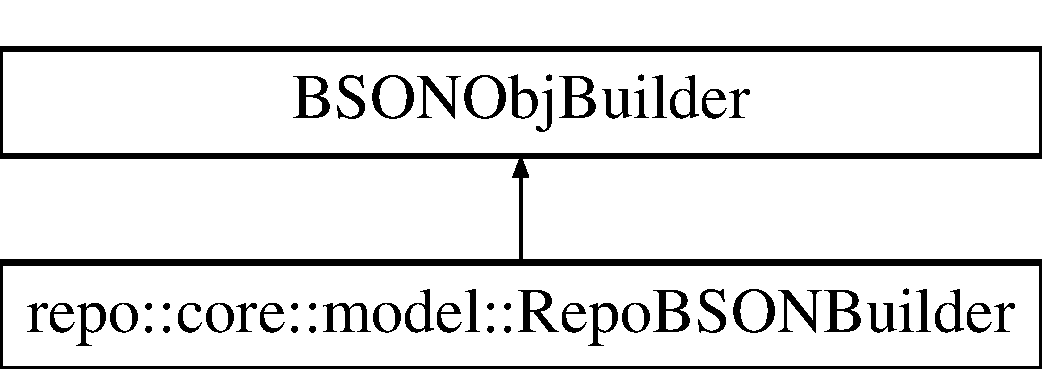
\includegraphics[height=2.000000cm]{classrepo_1_1core_1_1model_1_1_repo_b_s_o_n_builder}
\end{center}
\end{figure}
\subsection*{Public Member Functions}
\begin{DoxyCompactItemize}
\item 
{\footnotesize template$<$class T $>$ }\\void \hyperlink{classrepo_1_1core_1_1model_1_1_repo_b_s_o_n_builder_aac9e1ec05f85927b326da215e5505d94}{append\+Array} (const std\+::string \&label, const std\+::vector$<$ T $>$ \&vec)
\item 
\hypertarget{classrepo_1_1core_1_1model_1_1_repo_b_s_o_n_builder_ab0171c8ddcfc1064620085706ec80109}{}void {\bfseries append\+Array} (const std\+::string \&label, const \hyperlink{classrepo_1_1core_1_1model_1_1_repo_b_s_o_n}{Repo\+B\+S\+O\+N} \&bson)\label{classrepo_1_1core_1_1model_1_1_repo_b_s_o_n_builder_ab0171c8ddcfc1064620085706ec80109}

\item 
\hypertarget{classrepo_1_1core_1_1model_1_1_repo_b_s_o_n_builder_ac244225245e865c8bee66a56bcf4137a}{}{\footnotesize template$<$class T $>$ }\\void {\bfseries append} (const std\+::string \&label, const T \&item)\label{classrepo_1_1core_1_1model_1_1_repo_b_s_o_n_builder_ac244225245e865c8bee66a56bcf4137a}

\item 
void \hyperlink{classrepo_1_1core_1_1model_1_1_repo_b_s_o_n_builder_a21d4b0241bfc9d1c05cd7050d9b87b3e}{append\+Array\+Pair} (const std\+::string \&label, const std\+::list$<$ std\+::pair$<$ std\+::string, std\+::string $>$ $>$ \&list, const std\+::string \&fst\+Label, const std\+::string \&snd\+Label)
\item 
{\footnotesize template$<$class T $>$ }\\void \hyperlink{classrepo_1_1core_1_1model_1_1_repo_b_s_o_n_builder_aabe573365190367c7a3bd52692cd7a66}{append\+Binary} (const std\+::string \&label, const T $\ast$data, const uint32\+\_\+t \&byte\+Count)
\item 
\hypertarget{classrepo_1_1core_1_1model_1_1_repo_b_s_o_n_builder_ac886e9d0599b53c4bdf0bf00bfbf95da}{}void {\bfseries append\+Time\+Stamp} (std\+::string label)\label{classrepo_1_1core_1_1model_1_1_repo_b_s_o_n_builder_ac886e9d0599b53c4bdf0bf00bfbf95da}

\item 
\hypertarget{classrepo_1_1core_1_1model_1_1_repo_b_s_o_n_builder_a7797970aa65feafae46eaea2b4246c35}{}void {\bfseries append\+Time} (std\+::string label, const int64\+\_\+t \&ts)\label{classrepo_1_1core_1_1model_1_1_repo_b_s_o_n_builder_a7797970aa65feafae46eaea2b4246c35}

\item 
\hyperlink{classrepo_1_1core_1_1model_1_1_repo_b_s_o_n}{Repo\+B\+S\+O\+N} \hyperlink{classrepo_1_1core_1_1model_1_1_repo_b_s_o_n_builder_a8760ee2f38f05dbcc85ef2a6bb4cabfa}{obj} ()
\item 
\hypertarget{classrepo_1_1core_1_1model_1_1_repo_b_s_o_n_builder_ae0bb5dd33eb1342e27fc3b7dc201685f}{}{\footnotesize template$<$$>$ }\\void {\bfseries append} (const std\+::string \&label, const repo\+U\+U\+I\+D \&uuid)\label{classrepo_1_1core_1_1model_1_1_repo_b_s_o_n_builder_ae0bb5dd33eb1342e27fc3b7dc201685f}

\item 
\hypertarget{classrepo_1_1core_1_1model_1_1_repo_b_s_o_n_builder_ac4380c7a90c696c6e92b2c03123ff327}{}{\footnotesize template$<$$>$ }\\void {\bfseries append} (const std\+::string \&label, const \hyperlink{structrepo__vector__t}{repo\+\_\+vector\+\_\+t} \&vec)\label{classrepo_1_1core_1_1model_1_1_repo_b_s_o_n_builder_ac4380c7a90c696c6e92b2c03123ff327}

\item 
\hypertarget{classrepo_1_1core_1_1model_1_1_repo_b_s_o_n_builder_ae0bb5dd33eb1342e27fc3b7dc201685f}{}{\footnotesize template$<$$>$ }\\void {\bfseries append} (const std\+::string \&label, const repo\+U\+U\+I\+D \&uuid)\label{classrepo_1_1core_1_1model_1_1_repo_b_s_o_n_builder_ae0bb5dd33eb1342e27fc3b7dc201685f}

\item 
\hypertarget{classrepo_1_1core_1_1model_1_1_repo_b_s_o_n_builder_ac4380c7a90c696c6e92b2c03123ff327}{}{\footnotesize template$<$$>$ }\\void {\bfseries append} (const std\+::string \&label, const \hyperlink{structrepo__vector__t}{repo\+\_\+vector\+\_\+t} \&vec)\label{classrepo_1_1core_1_1model_1_1_repo_b_s_o_n_builder_ac4380c7a90c696c6e92b2c03123ff327}

\end{DoxyCompactItemize}


\subsection{Member Function Documentation}
\hypertarget{classrepo_1_1core_1_1model_1_1_repo_b_s_o_n_builder_aac9e1ec05f85927b326da215e5505d94}{}\index{repo\+::core\+::model\+::\+Repo\+B\+S\+O\+N\+Builder@{repo\+::core\+::model\+::\+Repo\+B\+S\+O\+N\+Builder}!append\+Array@{append\+Array}}
\index{append\+Array@{append\+Array}!repo\+::core\+::model\+::\+Repo\+B\+S\+O\+N\+Builder@{repo\+::core\+::model\+::\+Repo\+B\+S\+O\+N\+Builder}}
\subsubsection[{append\+Array}]{\setlength{\rightskip}{0pt plus 5cm}template$<$class T $>$ void repo\+::core\+::model\+::\+Repo\+B\+S\+O\+N\+Builder\+::append\+Array (
\begin{DoxyParamCaption}
\item[{const std\+::string \&}]{label, }
\item[{const std\+::vector$<$ T $>$ \&}]{vec}
\end{DoxyParamCaption}
)\hspace{0.3cm}{\ttfamily [inline]}}\label{classrepo_1_1core_1_1model_1_1_repo_b_s_o_n_builder_aac9e1ec05f85927b326da215e5505d94}
Append a vector as object into the bson This function creates an embedded \hyperlink{classrepo_1_1core_1_1model_1_1_repo_b_s_o_n}{Repo\+B\+S\+O\+N} and append that object as an array into the builder 
\begin{DoxyParams}{Parameters}
{\em label} & label of the array \\
\hline
{\em vec} & vector to append \\
\hline
\end{DoxyParams}
\hypertarget{classrepo_1_1core_1_1model_1_1_repo_b_s_o_n_builder_a21d4b0241bfc9d1c05cd7050d9b87b3e}{}\index{repo\+::core\+::model\+::\+Repo\+B\+S\+O\+N\+Builder@{repo\+::core\+::model\+::\+Repo\+B\+S\+O\+N\+Builder}!append\+Array\+Pair@{append\+Array\+Pair}}
\index{append\+Array\+Pair@{append\+Array\+Pair}!repo\+::core\+::model\+::\+Repo\+B\+S\+O\+N\+Builder@{repo\+::core\+::model\+::\+Repo\+B\+S\+O\+N\+Builder}}
\subsubsection[{append\+Array\+Pair}]{\setlength{\rightskip}{0pt plus 5cm}void Repo\+B\+S\+O\+N\+Builder\+::append\+Array\+Pair (
\begin{DoxyParamCaption}
\item[{const std\+::string \&}]{label, }
\item[{const std\+::list$<$ std\+::pair$<$ std\+::string, std\+::string $>$ $>$ \&}]{list, }
\item[{const std\+::string \&}]{fst\+Label, }
\item[{const std\+::string \&}]{snd\+Label}
\end{DoxyParamCaption}
)}\label{classrepo_1_1core_1_1model_1_1_repo_b_s_o_n_builder_a21d4b0241bfc9d1c05cd7050d9b87b3e}
Append a list of pairs into an arraybson of objects 
\begin{DoxyParams}{Parameters}
{\em label} & label to append the array against \\
\hline
{\em list} & list of pairs to append \\
\hline
{\em fst\+Label} & label for \#1 in the pair \\
\hline
{\em snd\+Label} & label for \#2 in the pair \\
\hline
\end{DoxyParams}
\hypertarget{classrepo_1_1core_1_1model_1_1_repo_b_s_o_n_builder_aabe573365190367c7a3bd52692cd7a66}{}\index{repo\+::core\+::model\+::\+Repo\+B\+S\+O\+N\+Builder@{repo\+::core\+::model\+::\+Repo\+B\+S\+O\+N\+Builder}!append\+Binary@{append\+Binary}}
\index{append\+Binary@{append\+Binary}!repo\+::core\+::model\+::\+Repo\+B\+S\+O\+N\+Builder@{repo\+::core\+::model\+::\+Repo\+B\+S\+O\+N\+Builder}}
\subsubsection[{append\+Binary}]{\setlength{\rightskip}{0pt plus 5cm}template$<$class T $>$ void repo\+::core\+::model\+::\+Repo\+B\+S\+O\+N\+Builder\+::append\+Binary (
\begin{DoxyParamCaption}
\item[{const std\+::string \&}]{label, }
\item[{const T $\ast$}]{data, }
\item[{const uint32\+\_\+t \&}]{byte\+Count}
\end{DoxyParamCaption}
)\hspace{0.3cm}{\ttfamily [inline]}}\label{classrepo_1_1core_1_1model_1_1_repo_b_s_o_n_builder_aabe573365190367c7a3bd52692cd7a66}
Appends a pointer to some memory as binary mongo\+::\+Bin\+Data\+General type array. Appends given data as a binary data blob into a given builder. Also appends the count of the elements and the byte count of the array if labels are specified 
\begin{DoxyParams}{Parameters}
{\em label} & Label for this element \\
\hline
{\em data} & the data itself \\
\hline
{\em byte\+Count} & size of data in bytes \\
\hline
{\em byte\+Count\+Label} & label to store byte\+Count \\
\hline
{\em count\+Label} & count label to store count \\
\hline
\end{DoxyParams}
\hypertarget{classrepo_1_1core_1_1model_1_1_repo_b_s_o_n_builder_a8760ee2f38f05dbcc85ef2a6bb4cabfa}{}\index{repo\+::core\+::model\+::\+Repo\+B\+S\+O\+N\+Builder@{repo\+::core\+::model\+::\+Repo\+B\+S\+O\+N\+Builder}!obj@{obj}}
\index{obj@{obj}!repo\+::core\+::model\+::\+Repo\+B\+S\+O\+N\+Builder@{repo\+::core\+::model\+::\+Repo\+B\+S\+O\+N\+Builder}}
\subsubsection[{obj}]{\setlength{\rightskip}{0pt plus 5cm}{\bf Repo\+B\+S\+O\+N} Repo\+B\+S\+O\+N\+Builder\+::obj (
\begin{DoxyParamCaption}
{}
\end{DoxyParamCaption}
)}\label{classrepo_1_1core_1_1model_1_1_repo_b_s_o_n_builder_a8760ee2f38f05dbcc85ef2a6bb4cabfa}
builds the B\+S\+O\+N object as \hyperlink{classrepo_1_1core_1_1model_1_1_repo_b_s_o_n}{Repo\+B\+S\+O\+N} given the information within the builder \begin{DoxyReturn}{Returns}
returns a \hyperlink{classrepo_1_1core_1_1model_1_1_repo_b_s_o_n}{Repo\+B\+S\+O\+N} object with the fields given. 
\end{DoxyReturn}


The documentation for this class was generated from the following files\+:\begin{DoxyCompactItemize}
\item 
C\+:/\+Users/\+Carmen/3\+D Repo/\+Repo/3drepobouncer/bouncer/src/repo/core/model/bson/repo\+\_\+bson\+\_\+builder.\+h\item 
C\+:/\+Users/\+Carmen/3\+D Repo/\+Repo/3drepobouncer/bouncer/src/repo/core/model/bson/repo\+\_\+bson\+\_\+builder.\+cpp\end{DoxyCompactItemize}

\hypertarget{classrepo_1_1core_1_1model_1_1_repo_b_s_o_n_element}{}\section{repo\+:\+:core\+:\+:model\+:\+:Repo\+B\+S\+O\+N\+Element Class Reference}
\label{classrepo_1_1core_1_1model_1_1_repo_b_s_o_n_element}\index{repo\+::core\+::model\+::\+Repo\+B\+S\+O\+N\+Element@{repo\+::core\+::model\+::\+Repo\+B\+S\+O\+N\+Element}}
Inheritance diagram for repo\+:\+:core\+:\+:model\+:\+:Repo\+B\+S\+O\+N\+Element\+:\begin{figure}[H]
\begin{center}
\leavevmode
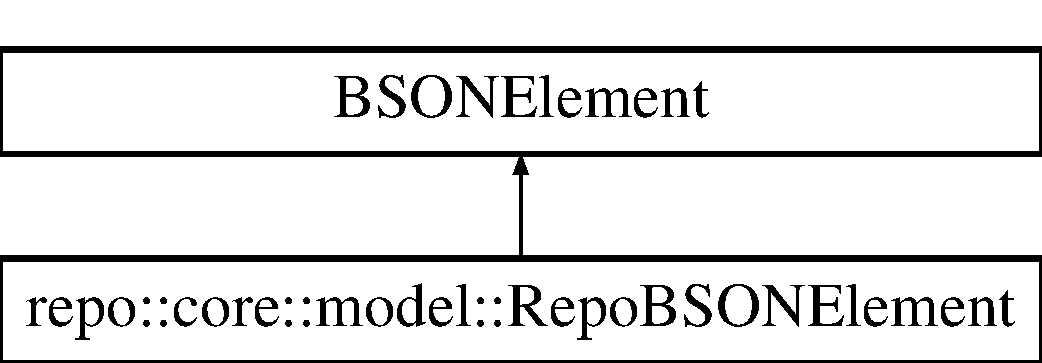
\includegraphics[height=2.000000cm]{classrepo_1_1core_1_1model_1_1_repo_b_s_o_n_element}
\end{center}
\end{figure}
\subsection*{Public Member Functions}
\begin{DoxyCompactItemize}
\item 
\hyperlink{classrepo_1_1core_1_1model_1_1_repo_b_s_o_n_element_ac90a539b9e6e62b6178f05dc8ca3449a}{Repo\+B\+S\+O\+N\+Element} ()
\item 
\hyperlink{classrepo_1_1core_1_1model_1_1_repo_b_s_o_n_element_a8739189159c94059b0aee8fc54824858}{Repo\+B\+S\+O\+N\+Element} (mongo\+::\+B\+S\+O\+N\+Element ele)
\item 
\hyperlink{classrepo_1_1core_1_1model_1_1_repo_b_s_o_n_element_aea7a17c6764257a19347bb4ff0897d12}{$\sim$\+Repo\+B\+S\+O\+N\+Element} ()
\item 
Element\+Type \hyperlink{classrepo_1_1core_1_1model_1_1_repo_b_s_o_n_element_ac267633e0b010be90a8041d0365c2b8d}{type} () const 
\item 
\hypertarget{classrepo_1_1core_1_1model_1_1_repo_b_s_o_n_element_afdd43bff95f977511151eb4e728d63e9}{}std\+::vector$<$ \hyperlink{classrepo_1_1core_1_1model_1_1_repo_b_s_o_n_element}{Repo\+B\+S\+O\+N\+Element} $>$ {\bfseries Array} ()\label{classrepo_1_1core_1_1model_1_1_repo_b_s_o_n_element_afdd43bff95f977511151eb4e728d63e9}

\end{DoxyCompactItemize}


\subsection{Constructor \& Destructor Documentation}
\hypertarget{classrepo_1_1core_1_1model_1_1_repo_b_s_o_n_element_ac90a539b9e6e62b6178f05dc8ca3449a}{}\index{repo\+::core\+::model\+::\+Repo\+B\+S\+O\+N\+Element@{repo\+::core\+::model\+::\+Repo\+B\+S\+O\+N\+Element}!Repo\+B\+S\+O\+N\+Element@{Repo\+B\+S\+O\+N\+Element}}
\index{Repo\+B\+S\+O\+N\+Element@{Repo\+B\+S\+O\+N\+Element}!repo\+::core\+::model\+::\+Repo\+B\+S\+O\+N\+Element@{repo\+::core\+::model\+::\+Repo\+B\+S\+O\+N\+Element}}
\subsubsection[{Repo\+B\+S\+O\+N\+Element}]{\setlength{\rightskip}{0pt plus 5cm}repo\+::core\+::model\+::\+Repo\+B\+S\+O\+N\+Element\+::\+Repo\+B\+S\+O\+N\+Element (
\begin{DoxyParamCaption}
{}
\end{DoxyParamCaption}
)\hspace{0.3cm}{\ttfamily [inline]}}\label{classrepo_1_1core_1_1model_1_1_repo_b_s_o_n_element_ac90a539b9e6e62b6178f05dc8ca3449a}
Default constructor \hypertarget{classrepo_1_1core_1_1model_1_1_repo_b_s_o_n_element_a8739189159c94059b0aee8fc54824858}{}\index{repo\+::core\+::model\+::\+Repo\+B\+S\+O\+N\+Element@{repo\+::core\+::model\+::\+Repo\+B\+S\+O\+N\+Element}!Repo\+B\+S\+O\+N\+Element@{Repo\+B\+S\+O\+N\+Element}}
\index{Repo\+B\+S\+O\+N\+Element@{Repo\+B\+S\+O\+N\+Element}!repo\+::core\+::model\+::\+Repo\+B\+S\+O\+N\+Element@{repo\+::core\+::model\+::\+Repo\+B\+S\+O\+N\+Element}}
\subsubsection[{Repo\+B\+S\+O\+N\+Element}]{\setlength{\rightskip}{0pt plus 5cm}repo\+::core\+::model\+::\+Repo\+B\+S\+O\+N\+Element\+::\+Repo\+B\+S\+O\+N\+Element (
\begin{DoxyParamCaption}
\item[{mongo\+::\+B\+S\+O\+N\+Element}]{ele}
\end{DoxyParamCaption}
)\hspace{0.3cm}{\ttfamily [inline]}}\label{classrepo_1_1core_1_1model_1_1_repo_b_s_o_n_element_a8739189159c94059b0aee8fc54824858}
Construct a \hyperlink{classrepo_1_1core_1_1model_1_1_repo_b_s_o_n_element}{Repo\+B\+S\+O\+N\+Element} base on a mongo element 
\begin{DoxyParams}{Parameters}
{\em mongo} & B\+S\+O\+N element \\
\hline
\end{DoxyParams}
\hypertarget{classrepo_1_1core_1_1model_1_1_repo_b_s_o_n_element_aea7a17c6764257a19347bb4ff0897d12}{}\index{repo\+::core\+::model\+::\+Repo\+B\+S\+O\+N\+Element@{repo\+::core\+::model\+::\+Repo\+B\+S\+O\+N\+Element}!````~Repo\+B\+S\+O\+N\+Element@{$\sim$\+Repo\+B\+S\+O\+N\+Element}}
\index{````~Repo\+B\+S\+O\+N\+Element@{$\sim$\+Repo\+B\+S\+O\+N\+Element}!repo\+::core\+::model\+::\+Repo\+B\+S\+O\+N\+Element@{repo\+::core\+::model\+::\+Repo\+B\+S\+O\+N\+Element}}
\subsubsection[{$\sim$\+Repo\+B\+S\+O\+N\+Element}]{\setlength{\rightskip}{0pt plus 5cm}Repo\+B\+S\+O\+N\+Element\+::$\sim$\+Repo\+B\+S\+O\+N\+Element (
\begin{DoxyParamCaption}
{}
\end{DoxyParamCaption}
)}\label{classrepo_1_1core_1_1model_1_1_repo_b_s_o_n_element_aea7a17c6764257a19347bb4ff0897d12}
Destructor 

\subsection{Member Function Documentation}
\hypertarget{classrepo_1_1core_1_1model_1_1_repo_b_s_o_n_element_ac267633e0b010be90a8041d0365c2b8d}{}\index{repo\+::core\+::model\+::\+Repo\+B\+S\+O\+N\+Element@{repo\+::core\+::model\+::\+Repo\+B\+S\+O\+N\+Element}!type@{type}}
\index{type@{type}!repo\+::core\+::model\+::\+Repo\+B\+S\+O\+N\+Element@{repo\+::core\+::model\+::\+Repo\+B\+S\+O\+N\+Element}}
\subsubsection[{type}]{\setlength{\rightskip}{0pt plus 5cm}Element\+Type Repo\+B\+S\+O\+N\+Element\+::type (
\begin{DoxyParamCaption}
{}
\end{DoxyParamCaption}
) const}\label{classrepo_1_1core_1_1model_1_1_repo_b_s_o_n_element_ac267633e0b010be90a8041d0365c2b8d}
get the type of the element \begin{DoxyReturn}{Returns}
returns the type of the element using enum Type specified above 
\end{DoxyReturn}


The documentation for this class was generated from the following files\+:\begin{DoxyCompactItemize}
\item 
C\+:/\+Users/\+Carmen/3\+D Repo/\+Repo/3drepobouncer/bouncer/src/repo/core/model/bson/repo\+\_\+bson\+\_\+element.\+h\item 
C\+:/\+Users/\+Carmen/3\+D Repo/\+Repo/3drepobouncer/bouncer/src/repo/core/model/bson/repo\+\_\+bson\+\_\+element.\+cpp\end{DoxyCompactItemize}

\hypertarget{classrepo_1_1core_1_1model_1_1_repo_b_s_o_n_factory}{}\section{repo\+:\+:core\+:\+:model\+:\+:Repo\+B\+S\+O\+N\+Factory Class Reference}
\label{classrepo_1_1core_1_1model_1_1_repo_b_s_o_n_factory}\index{repo\+::core\+::model\+::\+Repo\+B\+S\+O\+N\+Factory@{repo\+::core\+::model\+::\+Repo\+B\+S\+O\+N\+Factory}}
\subsection*{Static Public Member Functions}
\begin{DoxyCompactItemize}
\item 
static \hyperlink{classrepo_1_1core_1_1model_1_1_repo_project_settings}{Repo\+Project\+Settings} \hyperlink{classrepo_1_1core_1_1model_1_1_repo_b_s_o_n_factory_aaeeeab32a5d425b9c16ebdcbc423f1fe}{make\+Repo\+Project\+Settings} (const std\+::string \&unique\+Project\+Name, const std\+::string \&owner, const std\+::string \&type=R\+E\+P\+O\+\_\+\+D\+E\+F\+A\+U\+L\+T\+\_\+\+P\+R\+O\+J\+E\+C\+T\+\_\+\+T\+Y\+P\+E\+\_\+\+A\+R\+C\+H\+I\+T\+E\+C\+T\+U\+R\+A\+L, const std\+::string \&description=std\+::string(), const double pin\+Size=R\+E\+P\+O\+\_\+\+D\+E\+F\+A\+U\+L\+T\+\_\+\+P\+R\+O\+J\+E\+C\+T\+\_\+\+P\+I\+N\+\_\+\+S\+I\+Z\+E, const double avatar\+Height=R\+E\+P\+O\+\_\+\+D\+E\+F\+A\+U\+L\+T\+\_\+\+P\+R\+O\+J\+E\+C\+T\+\_\+\+A\+V\+A\+T\+A\+R\+\_\+\+H\+E\+I\+G\+H\+T, const double visibility\+Limit=R\+E\+P\+O\+\_\+\+D\+E\+F\+A\+U\+L\+T\+\_\+\+P\+R\+O\+J\+E\+C\+T\+\_\+\+V\+I\+S\+I\+B\+I\+L\+I\+T\+Y\+\_\+\+L\+I\+M\+I\+T, const double speed=R\+E\+P\+O\+\_\+\+D\+E\+F\+A\+U\+L\+T\+\_\+\+P\+R\+O\+J\+E\+C\+T\+\_\+\+S\+P\+E\+E\+D, const double z\+Near=R\+E\+P\+O\+\_\+\+D\+E\+F\+A\+U\+L\+T\+\_\+\+P\+R\+O\+J\+E\+C\+T\+\_\+\+Z\+N\+E\+A\+R, const double z\+Far=R\+E\+P\+O\+\_\+\+D\+E\+F\+A\+U\+L\+T\+\_\+\+P\+R\+O\+J\+E\+C\+T\+\_\+\+Z\+F\+A\+R)
\item 
static \hyperlink{classrepo_1_1core_1_1model_1_1_repo_role}{Repo\+Role} \hyperlink{classrepo_1_1core_1_1model_1_1_repo_b_s_o_n_factory_a6adaa268d88e85b45c461f2385715bf2}{make\+Repo\+Role} (const std\+::string \&role\+Name, const std\+::string \&database, const std\+::vector$<$ \hyperlink{structrepo_1_1core_1_1model_1_1_repo_permission}{Repo\+Permission} $>$ \&permissions=std\+::vector$<$ \hyperlink{structrepo_1_1core_1_1model_1_1_repo_permission}{Repo\+Permission} $>$(), const \hyperlink{classrepo_1_1core_1_1model_1_1_repo_role}{Repo\+Role} \&old\+Role=\hyperlink{classrepo_1_1core_1_1model_1_1_repo_role}{Repo\+Role}())
\item 
static \hyperlink{classrepo_1_1core_1_1model_1_1_repo_role}{Repo\+Role} \hyperlink{classrepo_1_1core_1_1model_1_1_repo_b_s_o_n_factory_a8dec46fa7f8dee1265f456d48e0e84e3}{\+\_\+make\+Repo\+Role} (const std\+::string \&role\+Name, const std\+::string \&database, const std\+::vector$<$ \hyperlink{structrepo_1_1core_1_1model_1_1_repo_privilege}{Repo\+Privilege} $>$ \&privileges, const std\+::vector$<$ std\+::pair$<$ std\+::string, std\+::string $>$$>$ \&inherited\+Roles=std\+::vector$<$ std\+::pair$<$ std\+::string, std\+::string $>$$>$())
\item 
\hypertarget{classrepo_1_1core_1_1model_1_1_repo_b_s_o_n_factory_a174cd12a456e0e16bba87c3fd0f44a3b}{}static \hyperlink{classrepo_1_1core_1_1model_1_1_repo_role_settings}{Repo\+Role\+Settings} {\bfseries make\+Repo\+Role\+Settings} (const std\+::string \&unique\+Role\+Name, const std\+::string \&color, const std\+::string \&description=std\+::string(), const std\+::vector$<$ std\+::string $>$ \&modules=std\+::vector$<$ std\+::string $>$())\label{classrepo_1_1core_1_1model_1_1_repo_b_s_o_n_factory_a174cd12a456e0e16bba87c3fd0f44a3b}

\item 
static \hyperlink{classrepo_1_1core_1_1model_1_1_repo_user}{Repo\+User} \hyperlink{classrepo_1_1core_1_1model_1_1_repo_b_s_o_n_factory_a71f31d9f55dd79764f955f113d0620a2}{make\+Repo\+User} (const std\+::string \&user\+Name, const std\+::string \&password, const std\+::string \&first\+Name, const std\+::string \&last\+Name, const std\+::string \&email, const std\+::list$<$ std\+::pair$<$ std\+::string, std\+::string $>$$>$ \&roles, const std\+::list$<$ std\+::pair$<$ std\+::string, std\+::string $>$$>$ \&api\+Keys, const std\+::vector$<$ char $>$ \&avatar)
\item 
static \hyperlink{classrepo_1_1core_1_1model_1_1_repo_b_s_o_n}{Repo\+B\+S\+O\+N} \hyperlink{classrepo_1_1core_1_1model_1_1_repo_b_s_o_n_factory_addddc912d9cda2582e39689832c67c64}{append\+Defaults} (const std\+::string \&type, const unsigned int api=R\+E\+P\+O\+\_\+\+N\+O\+D\+E\+\_\+\+A\+P\+I\+\_\+\+L\+E\+V\+E\+L\+\_\+0, const repo\+U\+U\+I\+D \&shared\+Id=generate\+U\+U\+I\+D(), const std\+::string \&name=std\+::string(), const std\+::vector$<$ repo\+U\+U\+I\+D $>$ \&parents=std\+::vector$<$ repo\+U\+U\+I\+D $>$(), const repo\+U\+U\+I\+D \&unique\+I\+D=generate\+U\+U\+I\+D())
\item 
static \hyperlink{classrepo_1_1core_1_1model_1_1_camera_node}{Camera\+Node} \hyperlink{classrepo_1_1core_1_1model_1_1_repo_b_s_o_n_factory_a23353f1a12968ec60bcd7013df3dd1dc}{make\+Camera\+Node} (const float \&aspect\+Ratio, const float \&far\+Clipping\+Plane, const float \&near\+Clipping\+Plane, const float \&field\+Of\+View, const \hyperlink{structrepo__vector__t}{repo\+\_\+vector\+\_\+t} \&look\+At, const \hyperlink{structrepo__vector__t}{repo\+\_\+vector\+\_\+t} \&position, const \hyperlink{structrepo__vector__t}{repo\+\_\+vector\+\_\+t} \&up, const std\+::string \&name=std\+::string(), const int \&api\+Level=R\+E\+P\+O\+\_\+\+N\+O\+D\+E\+\_\+\+A\+P\+I\+\_\+\+L\+E\+V\+E\+L\+\_\+1)
\item 
static \hyperlink{classrepo_1_1core_1_1model_1_1_material_node}{Material\+Node} \hyperlink{classrepo_1_1core_1_1model_1_1_repo_b_s_o_n_factory_a045a2f1546300e6de1590ca4c0200050}{make\+Material\+Node} (const \hyperlink{structrepo__material__t}{repo\+\_\+material\+\_\+t} \&material, const std\+::string \&name=std\+::string(), const int \&api\+Level=R\+E\+P\+O\+\_\+\+N\+O\+D\+E\+\_\+\+A\+P\+I\+\_\+\+L\+E\+V\+E\+L\+\_\+1)
\item 
static \hyperlink{classrepo_1_1core_1_1model_1_1_map_node}{Map\+Node} \hyperlink{classrepo_1_1core_1_1model_1_1_repo_b_s_o_n_factory_ad675c473a8b9c34445bb3da33e7976bf}{make\+Map\+Node} (const uint32\+\_\+t \&width, const uint32\+\_\+t \&zoom, const float \&tilt, const float \&tile\+Size, const float \&longitude, const float \&latitude, const \hyperlink{structrepo__vector__t}{repo\+\_\+vector\+\_\+t} \&centre\+Point, const std\+::string \&api\+Key=std\+::string(), const std\+::string \&name=std\+::string(), const int \&api\+Level=R\+E\+P\+O\+\_\+\+N\+O\+D\+E\+\_\+\+A\+P\+I\+\_\+\+L\+E\+V\+E\+L\+\_\+1)
\item 
static \hyperlink{classrepo_1_1core_1_1model_1_1_metadata_node}{Metadata\+Node} \hyperlink{classrepo_1_1core_1_1model_1_1_repo_b_s_o_n_factory_ad9f35349bdd78f2875797b86e372ffbd}{make\+Meta\+Data\+Node} (\hyperlink{classrepo_1_1core_1_1model_1_1_repo_b_s_o_n}{Repo\+B\+S\+O\+N} \&metadata, const std\+::string \&mime\+Type=std\+::string(), const std\+::string \&name=std\+::string(), const std\+::vector$<$ repo\+U\+U\+I\+D $>$ \&parents=std\+::vector$<$ repo\+U\+U\+I\+D $>$(), const int \&api\+Level=R\+E\+P\+O\+\_\+\+N\+O\+D\+E\+\_\+\+A\+P\+I\+\_\+\+L\+E\+V\+E\+L\+\_\+1)
\item 
static \hyperlink{classrepo_1_1core_1_1model_1_1_metadata_node}{Metadata\+Node} \hyperlink{classrepo_1_1core_1_1model_1_1_repo_b_s_o_n_factory_a3ab71e1eae99cd29785ad50cd02e7d19}{make\+Meta\+Data\+Node} (const std\+::vector$<$ std\+::string $>$ \&keys, const std\+::vector$<$ std\+::string $>$ \&values, const std\+::string \&name=std\+::string(), const std\+::vector$<$ repo\+U\+U\+I\+D $>$ \&parents=std\+::vector$<$ repo\+U\+U\+I\+D $>$(), const int \&api\+Level=R\+E\+P\+O\+\_\+\+N\+O\+D\+E\+\_\+\+A\+P\+I\+\_\+\+L\+E\+V\+E\+L\+\_\+1)
\item 
static \hyperlink{classrepo_1_1core_1_1model_1_1_mesh_node}{Mesh\+Node} \hyperlink{classrepo_1_1core_1_1model_1_1_repo_b_s_o_n_factory_a27372207255a35ee815109843fb21543}{make\+Mesh\+Node} (const std\+::vector$<$ \hyperlink{structrepo__vector__t}{repo\+\_\+vector\+\_\+t} $>$ \&vertices, const std\+::vector$<$ repo\+\_\+face\+\_\+t $>$ \&faces, const std\+::vector$<$ \hyperlink{structrepo__vector__t}{repo\+\_\+vector\+\_\+t} $>$ \&normals, const std\+::vector$<$ std\+::vector$<$ float $>$$>$ \&bounding\+Box, const std\+::vector$<$ std\+::vector$<$ \hyperlink{structrepo__vector2d__t}{repo\+\_\+vector2d\+\_\+t} $>$$>$ \&uv\+Channels=std\+::vector$<$ std\+::vector$<$ \hyperlink{structrepo__vector2d__t}{repo\+\_\+vector2d\+\_\+t} $>$$>$(), const std\+::vector$<$ \hyperlink{structrepo__color4d__t}{repo\+\_\+color4d\+\_\+t} $>$ \&colors=std\+::vector$<$ \hyperlink{structrepo__color4d__t}{repo\+\_\+color4d\+\_\+t} $>$(), const std\+::vector$<$ std\+::vector$<$ float $>$$>$ \&outline=std\+::vector$<$ std\+::vector$<$ float $>$$>$(), const std\+::string \&name=std\+::string(), const int \&api\+Level=R\+E\+P\+O\+\_\+\+N\+O\+D\+E\+\_\+\+A\+P\+I\+\_\+\+L\+E\+V\+E\+L\+\_\+1)
\item 
static \hyperlink{classrepo_1_1core_1_1model_1_1_reference_node}{Reference\+Node} \hyperlink{classrepo_1_1core_1_1model_1_1_repo_b_s_o_n_factory_a788b309527ef6b00fba0ba8531e1f481}{make\+Reference\+Node} (const std\+::string \&database, const std\+::string \&project, const repo\+U\+U\+I\+D \&revision\+I\+D=string\+To\+U\+U\+I\+D(R\+E\+P\+O\+\_\+\+H\+I\+S\+T\+O\+R\+Y\+\_\+\+M\+A\+S\+T\+E\+R\+\_\+\+B\+R\+A\+N\+C\+H), const bool \&is\+Unique\+I\+D=false, const std\+::string \&name=std\+::string(), const int \&api\+Level=R\+E\+P\+O\+\_\+\+N\+O\+D\+E\+\_\+\+A\+P\+I\+\_\+\+L\+E\+V\+E\+L\+\_\+1)
\item 
static \hyperlink{classrepo_1_1core_1_1model_1_1_revision_node}{Revision\+Node} \hyperlink{classrepo_1_1core_1_1model_1_1_repo_b_s_o_n_factory_a09da9eaea3d86630fa98836c31499019}{make\+Revision\+Node} (const std\+::string \&user, const repo\+U\+U\+I\+D \&branch, const std\+::vector$<$ repo\+U\+U\+I\+D $>$ \&current\+Nodes, const std\+::vector$<$ std\+::string $>$ \&files=std\+::vector$<$ std\+::string $>$(), const std\+::vector$<$ repo\+U\+U\+I\+D $>$ \&parent=std\+::vector$<$ repo\+U\+U\+I\+D $>$(), const std\+::vector$<$ double $>$ \&world\+Offset=std\+::vector$<$ double $>$(), const std\+::string \&message=std\+::string(), const std\+::string \&tag=std\+::string(), const int \&api\+Level=R\+E\+P\+O\+\_\+\+N\+O\+D\+E\+\_\+\+A\+P\+I\+\_\+\+L\+E\+V\+E\+L\+\_\+1)
\item 
static \hyperlink{classrepo_1_1core_1_1model_1_1_texture_node}{Texture\+Node} \hyperlink{classrepo_1_1core_1_1model_1_1_repo_b_s_o_n_factory_ab8368070b611929c37d235ef4142d34b}{make\+Texture\+Node} (const std\+::string \&name, const char $\ast$data, const uint32\+\_\+t \&byte\+Count, const uint32\+\_\+t \&width, const uint32\+\_\+t \&height, const int \&api\+Level=R\+E\+P\+O\+\_\+\+N\+O\+D\+E\+\_\+\+A\+P\+I\+\_\+\+L\+E\+V\+E\+L\+\_\+1)
\item 
static \hyperlink{classrepo_1_1core_1_1model_1_1_transformation_node}{Transformation\+Node} \hyperlink{classrepo_1_1core_1_1model_1_1_repo_b_s_o_n_factory_a2f793553bccd5b53a4814ac438680651}{make\+Transformation\+Node} (const std\+::vector$<$ std\+::vector$<$ float $>$$>$ \&trans\+Matrix=\hyperlink{classrepo_1_1core_1_1model_1_1_transformation_node_ac6723324b4ef9d6c0aacf53572a46d7f}{Transformation\+Node\+::identity\+Mat}(), const std\+::string \&name=\char`\"{}$<$transformation$>$\char`\"{}, const std\+::vector$<$ repo\+U\+U\+I\+D $>$ \&parents=std\+::vector$<$ repo\+U\+U\+I\+D $>$(), const int \&api\+Level=R\+E\+P\+O\+\_\+\+N\+O\+D\+E\+\_\+\+A\+P\+I\+\_\+\+L\+E\+V\+E\+L\+\_\+1)
\end{DoxyCompactItemize}


\subsection{Member Function Documentation}
\hypertarget{classrepo_1_1core_1_1model_1_1_repo_b_s_o_n_factory_a8dec46fa7f8dee1265f456d48e0e84e3}{}\index{repo\+::core\+::model\+::\+Repo\+B\+S\+O\+N\+Factory@{repo\+::core\+::model\+::\+Repo\+B\+S\+O\+N\+Factory}!\+\_\+make\+Repo\+Role@{\+\_\+make\+Repo\+Role}}
\index{\+\_\+make\+Repo\+Role@{\+\_\+make\+Repo\+Role}!repo\+::core\+::model\+::\+Repo\+B\+S\+O\+N\+Factory@{repo\+::core\+::model\+::\+Repo\+B\+S\+O\+N\+Factory}}
\subsubsection[{\+\_\+make\+Repo\+Role}]{\setlength{\rightskip}{0pt plus 5cm}{\bf Repo\+Role} Repo\+B\+S\+O\+N\+Factory\+::\+\_\+make\+Repo\+Role (
\begin{DoxyParamCaption}
\item[{const std\+::string \&}]{role\+Name, }
\item[{const std\+::string \&}]{database, }
\item[{const std\+::vector$<$ {\bf Repo\+Privilege} $>$ \&}]{privileges, }
\item[{const std\+::vector$<$ std\+::pair$<$ std\+::string, std\+::string $>$$>$ \&}]{inherited\+Roles = {\ttfamily std\+:\+:vector$<$std\+:\+:pair$<$std\+:\+:string,~std\+:\+:string$>$$>$()}}
\end{DoxyParamCaption}
)\hspace{0.3cm}{\ttfamily [static]}}\label{classrepo_1_1core_1_1model_1_1_repo_b_s_o_n_factory_a8dec46fa7f8dee1265f456d48e0e84e3}
Create a role B\+S\+O\+N 
\begin{DoxyParams}{Parameters}
{\em role\+Name} & name of the role \\
\hline
{\em database} & database where this role resides \\
\hline
{\em privileges} & a vector of privileges this role has \\
\hline
{\em inherted\+Roles} & vector of roles which this role inherits from \\
\hline
\end{DoxyParams}
\begin{DoxyReturn}{Returns}
returns a bson with this role information 
\end{DoxyReturn}
\hypertarget{classrepo_1_1core_1_1model_1_1_repo_b_s_o_n_factory_addddc912d9cda2582e39689832c67c64}{}\index{repo\+::core\+::model\+::\+Repo\+B\+S\+O\+N\+Factory@{repo\+::core\+::model\+::\+Repo\+B\+S\+O\+N\+Factory}!append\+Defaults@{append\+Defaults}}
\index{append\+Defaults@{append\+Defaults}!repo\+::core\+::model\+::\+Repo\+B\+S\+O\+N\+Factory@{repo\+::core\+::model\+::\+Repo\+B\+S\+O\+N\+Factory}}
\subsubsection[{append\+Defaults}]{\setlength{\rightskip}{0pt plus 5cm}{\bf Repo\+B\+S\+O\+N} Repo\+B\+S\+O\+N\+Factory\+::append\+Defaults (
\begin{DoxyParamCaption}
\item[{const std\+::string \&}]{type, }
\item[{const unsigned int}]{api = {\ttfamily REPO\+\_\+NODE\+\_\+API\+\_\+LEVEL\+\_\+0}, }
\item[{const repo\+U\+U\+I\+D \&}]{shared\+Id = {\ttfamily generateUUID()}, }
\item[{const std\+::string \&}]{name = {\ttfamily std\+:\+:string()}, }
\item[{const std\+::vector$<$ repo\+U\+U\+I\+D $>$ \&}]{parents = {\ttfamily std\+:\+:vector$<$repoUUID$>$()}, }
\item[{const repo\+U\+U\+I\+D \&}]{unique\+I\+D = {\ttfamily generateUUID()}}
\end{DoxyParamCaption}
)\hspace{0.3cm}{\ttfamily [static]}}\label{classrepo_1_1core_1_1model_1_1_repo_b_s_o_n_factory_addddc912d9cda2582e39689832c67c64}
Append default information onto the a \hyperlink{classrepo_1_1core_1_1model_1_1_repo_b_s_o_n_builder}{Repo\+B\+S\+O\+N\+Builder} This is used for children nodes to create their B\+S\+O\+Ns. 
\begin{DoxyParams}{Parameters}
{\em type} & type of node \\
\hline
{\em api} & api level of this node \\
\hline
{\em share\+I\+D} & shared I\+D of this node \\
\hline
{\em name} & name of the node \\
\hline
{\em parents} & vector of shared I\+Ds of this node\textquotesingle{}s parents \\
\hline
{\em unique\+I\+D} & specify unique I\+D for the object (do not use unless you are sure you know what you\textquotesingle{}re doing!) @ return return a bson object with the default parameters \\
\hline
\end{DoxyParams}
\hypertarget{classrepo_1_1core_1_1model_1_1_repo_b_s_o_n_factory_a23353f1a12968ec60bcd7013df3dd1dc}{}\index{repo\+::core\+::model\+::\+Repo\+B\+S\+O\+N\+Factory@{repo\+::core\+::model\+::\+Repo\+B\+S\+O\+N\+Factory}!make\+Camera\+Node@{make\+Camera\+Node}}
\index{make\+Camera\+Node@{make\+Camera\+Node}!repo\+::core\+::model\+::\+Repo\+B\+S\+O\+N\+Factory@{repo\+::core\+::model\+::\+Repo\+B\+S\+O\+N\+Factory}}
\subsubsection[{make\+Camera\+Node}]{\setlength{\rightskip}{0pt plus 5cm}{\bf Camera\+Node} Repo\+B\+S\+O\+N\+Factory\+::make\+Camera\+Node (
\begin{DoxyParamCaption}
\item[{const float \&}]{aspect\+Ratio, }
\item[{const float \&}]{far\+Clipping\+Plane, }
\item[{const float \&}]{near\+Clipping\+Plane, }
\item[{const float \&}]{field\+Of\+View, }
\item[{const {\bf repo\+\_\+vector\+\_\+t} \&}]{look\+At, }
\item[{const {\bf repo\+\_\+vector\+\_\+t} \&}]{position, }
\item[{const {\bf repo\+\_\+vector\+\_\+t} \&}]{up, }
\item[{const std\+::string \&}]{name = {\ttfamily std\+:\+:string()}, }
\item[{const int \&}]{api\+Level = {\ttfamily REPO\+\_\+NODE\+\_\+API\+\_\+LEVEL\+\_\+1}}
\end{DoxyParamCaption}
)\hspace{0.3cm}{\ttfamily [static]}}\label{classrepo_1_1core_1_1model_1_1_repo_b_s_o_n_factory_a23353f1a12968ec60bcd7013df3dd1dc}
Create a Camera Node 
\begin{DoxyParams}{Parameters}
{\em aspect} & ratio \\
\hline
{\em Far} & clipping plane \\
\hline
{\em Near} & clipping plane. Should not be 0 to avoid divis \\
\hline
{\em Field} & of view. \\
\hline
{\em Look\+At} & vector relative to parent transformations. \\
\hline
{\em Position} & relative to parent transformations \\
\hline
{\em Up} & vector relative to parent transformations. \\
\hline
{\em A\+P\+I} & level of the node (optional, default R\+E\+P\+O\+\_\+\+N\+O\+D\+E\+\_\+\+A\+P\+I\+\_\+\+L\+E\+V\+E\+L\+\_\+1) \\
\hline
{\em name} & of the node (optional, default empty string) \\
\hline
\end{DoxyParams}
\begin{DoxyReturn}{Returns}
returns a Camera node 
\end{DoxyReturn}
\hypertarget{classrepo_1_1core_1_1model_1_1_repo_b_s_o_n_factory_ad675c473a8b9c34445bb3da33e7976bf}{}\index{repo\+::core\+::model\+::\+Repo\+B\+S\+O\+N\+Factory@{repo\+::core\+::model\+::\+Repo\+B\+S\+O\+N\+Factory}!make\+Map\+Node@{make\+Map\+Node}}
\index{make\+Map\+Node@{make\+Map\+Node}!repo\+::core\+::model\+::\+Repo\+B\+S\+O\+N\+Factory@{repo\+::core\+::model\+::\+Repo\+B\+S\+O\+N\+Factory}}
\subsubsection[{make\+Map\+Node}]{\setlength{\rightskip}{0pt plus 5cm}{\bf Map\+Node} Repo\+B\+S\+O\+N\+Factory\+::make\+Map\+Node (
\begin{DoxyParamCaption}
\item[{const uint32\+\_\+t \&}]{width, }
\item[{const uint32\+\_\+t \&}]{zoom, }
\item[{const float \&}]{tilt, }
\item[{const float \&}]{tile\+Size, }
\item[{const float \&}]{longitude, }
\item[{const float \&}]{latitude, }
\item[{const {\bf repo\+\_\+vector\+\_\+t} \&}]{centre\+Point, }
\item[{const std\+::string \&}]{api\+Key = {\ttfamily std\+:\+:string()}, }
\item[{const std\+::string \&}]{name = {\ttfamily std\+:\+:string()}, }
\item[{const int \&}]{api\+Level = {\ttfamily REPO\+\_\+NODE\+\_\+API\+\_\+LEVEL\+\_\+1}}
\end{DoxyParamCaption}
)\hspace{0.3cm}{\ttfamily [static]}}\label{classrepo_1_1core_1_1model_1_1_repo_b_s_o_n_factory_ad675c473a8b9c34445bb3da33e7976bf}
Create a Map Node 
\begin{DoxyParams}{Parameters}
{\em a} & struct that contains the info about the material \\
\hline
{\em name} & of the Map \\
\hline
\end{DoxyParams}
\begin{DoxyReturn}{Returns}
returns a Map node 
\end{DoxyReturn}
\hypertarget{classrepo_1_1core_1_1model_1_1_repo_b_s_o_n_factory_a045a2f1546300e6de1590ca4c0200050}{}\index{repo\+::core\+::model\+::\+Repo\+B\+S\+O\+N\+Factory@{repo\+::core\+::model\+::\+Repo\+B\+S\+O\+N\+Factory}!make\+Material\+Node@{make\+Material\+Node}}
\index{make\+Material\+Node@{make\+Material\+Node}!repo\+::core\+::model\+::\+Repo\+B\+S\+O\+N\+Factory@{repo\+::core\+::model\+::\+Repo\+B\+S\+O\+N\+Factory}}
\subsubsection[{make\+Material\+Node}]{\setlength{\rightskip}{0pt plus 5cm}{\bf Material\+Node} Repo\+B\+S\+O\+N\+Factory\+::make\+Material\+Node (
\begin{DoxyParamCaption}
\item[{const {\bf repo\+\_\+material\+\_\+t} \&}]{material, }
\item[{const std\+::string \&}]{name = {\ttfamily std\+:\+:string()}, }
\item[{const int \&}]{api\+Level = {\ttfamily REPO\+\_\+NODE\+\_\+API\+\_\+LEVEL\+\_\+1}}
\end{DoxyParamCaption}
)\hspace{0.3cm}{\ttfamily [static]}}\label{classrepo_1_1core_1_1model_1_1_repo_b_s_o_n_factory_a045a2f1546300e6de1590ca4c0200050}
Create a Material Node 
\begin{DoxyParams}{Parameters}
{\em a} & struct that contains the info about the material \\
\hline
{\em name} & of the Material \\
\hline
\end{DoxyParams}
\begin{DoxyReturn}{Returns}
returns a Material node 
\end{DoxyReturn}
\hypertarget{classrepo_1_1core_1_1model_1_1_repo_b_s_o_n_factory_a27372207255a35ee815109843fb21543}{}\index{repo\+::core\+::model\+::\+Repo\+B\+S\+O\+N\+Factory@{repo\+::core\+::model\+::\+Repo\+B\+S\+O\+N\+Factory}!make\+Mesh\+Node@{make\+Mesh\+Node}}
\index{make\+Mesh\+Node@{make\+Mesh\+Node}!repo\+::core\+::model\+::\+Repo\+B\+S\+O\+N\+Factory@{repo\+::core\+::model\+::\+Repo\+B\+S\+O\+N\+Factory}}
\subsubsection[{make\+Mesh\+Node}]{\setlength{\rightskip}{0pt plus 5cm}{\bf Mesh\+Node} Repo\+B\+S\+O\+N\+Factory\+::make\+Mesh\+Node (
\begin{DoxyParamCaption}
\item[{const std\+::vector$<$ {\bf repo\+\_\+vector\+\_\+t} $>$ \&}]{vertices, }
\item[{const std\+::vector$<$ repo\+\_\+face\+\_\+t $>$ \&}]{faces, }
\item[{const std\+::vector$<$ {\bf repo\+\_\+vector\+\_\+t} $>$ \&}]{normals, }
\item[{const std\+::vector$<$ std\+::vector$<$ float $>$$>$ \&}]{bounding\+Box, }
\item[{const std\+::vector$<$ std\+::vector$<$ {\bf repo\+\_\+vector2d\+\_\+t} $>$$>$ \&}]{uv\+Channels = {\ttfamily std\+:\+:vector$<$std\+:\+:vector$<${\bf repo\+\_\+vector2d\+\_\+t}$>$$>$()}, }
\item[{const std\+::vector$<$ {\bf repo\+\_\+color4d\+\_\+t} $>$ \&}]{colors = {\ttfamily std\+:\+:vector$<${\bf repo\+\_\+color4d\+\_\+t}$>$()}, }
\item[{const std\+::vector$<$ std\+::vector$<$ float $>$$>$ \&}]{outline = {\ttfamily std\+:\+:vector$<$std\+:\+:vector$<$float$>$$>$()}, }
\item[{const std\+::string \&}]{name = {\ttfamily std\+:\+:string()}, }
\item[{const int \&}]{api\+Level = {\ttfamily REPO\+\_\+NODE\+\_\+API\+\_\+LEVEL\+\_\+1}}
\end{DoxyParamCaption}
)\hspace{0.3cm}{\ttfamily [static]}}\label{classrepo_1_1core_1_1model_1_1_repo_b_s_o_n_factory_a27372207255a35ee815109843fb21543}
Create a Mesh Node 
\begin{DoxyParams}{Parameters}
{\em vertices} & vector of vertices \\
\hline
{\em faces} & vector of faces \\
\hline
{\em normals} & vector of normals \\
\hline
{\em bounding\+Box} & vector of 2 vertex indicating the bounding box \\
\hline
{\em uv\+Channels} & vector of U\+V Channels \\
\hline
{\em colors} & vector of colours \\
\hline
{\em outline} & outline generated from bounding box \\
\hline
{\em name} & name of the node (optional, default empty string) \\
\hline
{\em api\+Level} & A\+P\+I level of the node (optional, default R\+E\+P\+O\+\_\+\+N\+O\+D\+E\+\_\+\+A\+P\+I\+\_\+\+L\+E\+V\+E\+L\+\_\+1) \\
\hline
\end{DoxyParams}
\begin{DoxyReturn}{Returns}
returns a mesh node 
\end{DoxyReturn}
\hypertarget{classrepo_1_1core_1_1model_1_1_repo_b_s_o_n_factory_ad9f35349bdd78f2875797b86e372ffbd}{}\index{repo\+::core\+::model\+::\+Repo\+B\+S\+O\+N\+Factory@{repo\+::core\+::model\+::\+Repo\+B\+S\+O\+N\+Factory}!make\+Meta\+Data\+Node@{make\+Meta\+Data\+Node}}
\index{make\+Meta\+Data\+Node@{make\+Meta\+Data\+Node}!repo\+::core\+::model\+::\+Repo\+B\+S\+O\+N\+Factory@{repo\+::core\+::model\+::\+Repo\+B\+S\+O\+N\+Factory}}
\subsubsection[{make\+Meta\+Data\+Node}]{\setlength{\rightskip}{0pt plus 5cm}{\bf Metadata\+Node} Repo\+B\+S\+O\+N\+Factory\+::make\+Meta\+Data\+Node (
\begin{DoxyParamCaption}
\item[{{\bf Repo\+B\+S\+O\+N} \&}]{metadata, }
\item[{const std\+::string \&}]{mime\+Type = {\ttfamily std\+:\+:string()}, }
\item[{const std\+::string \&}]{name = {\ttfamily std\+:\+:string()}, }
\item[{const std\+::vector$<$ repo\+U\+U\+I\+D $>$ \&}]{parents = {\ttfamily std\+:\+:vector$<$repoUUID$>$()}, }
\item[{const int \&}]{api\+Level = {\ttfamily REPO\+\_\+NODE\+\_\+API\+\_\+LEVEL\+\_\+1}}
\end{DoxyParamCaption}
)\hspace{0.3cm}{\ttfamily [static]}}\label{classrepo_1_1core_1_1model_1_1_repo_b_s_o_n_factory_ad9f35349bdd78f2875797b86e372ffbd}
Create a Metadata Node 
\begin{DoxyParams}{Parameters}
{\em metadata} & Metadata itself in \hyperlink{classrepo_1_1core_1_1model_1_1_repo_b_s_o_n}{Repo\+B\+S\+O\+N} format \\
\hline
{\em mimtype} & Mime type, the media type of the metadata (optional) \\
\hline
{\em name} & Name of Metadata (optional) \\
\hline
{\em parents} & \\
\hline
{\em api\+Level} & Repo Node A\+P\+I level (optional) \\
\hline
\end{DoxyParams}
\begin{DoxyReturn}{Returns}
returns a metadata node 
\end{DoxyReturn}
\hypertarget{classrepo_1_1core_1_1model_1_1_repo_b_s_o_n_factory_a3ab71e1eae99cd29785ad50cd02e7d19}{}\index{repo\+::core\+::model\+::\+Repo\+B\+S\+O\+N\+Factory@{repo\+::core\+::model\+::\+Repo\+B\+S\+O\+N\+Factory}!make\+Meta\+Data\+Node@{make\+Meta\+Data\+Node}}
\index{make\+Meta\+Data\+Node@{make\+Meta\+Data\+Node}!repo\+::core\+::model\+::\+Repo\+B\+S\+O\+N\+Factory@{repo\+::core\+::model\+::\+Repo\+B\+S\+O\+N\+Factory}}
\subsubsection[{make\+Meta\+Data\+Node}]{\setlength{\rightskip}{0pt plus 5cm}{\bf Metadata\+Node} Repo\+B\+S\+O\+N\+Factory\+::make\+Meta\+Data\+Node (
\begin{DoxyParamCaption}
\item[{const std\+::vector$<$ std\+::string $>$ \&}]{keys, }
\item[{const std\+::vector$<$ std\+::string $>$ \&}]{values, }
\item[{const std\+::string \&}]{name = {\ttfamily std\+:\+:string()}, }
\item[{const std\+::vector$<$ repo\+U\+U\+I\+D $>$ \&}]{parents = {\ttfamily std\+:\+:vector$<$repoUUID$>$()}, }
\item[{const int \&}]{api\+Level = {\ttfamily REPO\+\_\+NODE\+\_\+API\+\_\+LEVEL\+\_\+1}}
\end{DoxyParamCaption}
)\hspace{0.3cm}{\ttfamily [static]}}\label{classrepo_1_1core_1_1model_1_1_repo_b_s_o_n_factory_a3ab71e1eae99cd29785ad50cd02e7d19}
Create a Metadata Node 
\begin{DoxyParams}{Parameters}
{\em keys} & labels for the fields \\
\hline
{\em values} & values of the fields, matching the key parameter \\
\hline
{\em name} & Name of Metadata (optional) \\
\hline
{\em parents} & \\
\hline
{\em api\+Level} & Repo Node A\+P\+I level (optional) \\
\hline
\end{DoxyParams}
\begin{DoxyReturn}{Returns}
returns a metadata node 
\end{DoxyReturn}
\hypertarget{classrepo_1_1core_1_1model_1_1_repo_b_s_o_n_factory_a788b309527ef6b00fba0ba8531e1f481}{}\index{repo\+::core\+::model\+::\+Repo\+B\+S\+O\+N\+Factory@{repo\+::core\+::model\+::\+Repo\+B\+S\+O\+N\+Factory}!make\+Reference\+Node@{make\+Reference\+Node}}
\index{make\+Reference\+Node@{make\+Reference\+Node}!repo\+::core\+::model\+::\+Repo\+B\+S\+O\+N\+Factory@{repo\+::core\+::model\+::\+Repo\+B\+S\+O\+N\+Factory}}
\subsubsection[{make\+Reference\+Node}]{\setlength{\rightskip}{0pt plus 5cm}{\bf Reference\+Node} Repo\+B\+S\+O\+N\+Factory\+::make\+Reference\+Node (
\begin{DoxyParamCaption}
\item[{const std\+::string \&}]{database, }
\item[{const std\+::string \&}]{project, }
\item[{const repo\+U\+U\+I\+D \&}]{revision\+I\+D = {\ttfamily stringToUUID(REPO\+\_\+HISTORY\+\_\+MASTER\+\_\+BRANCH)}, }
\item[{const bool \&}]{is\+Unique\+I\+D = {\ttfamily false}, }
\item[{const std\+::string \&}]{name = {\ttfamily std\+:\+:string()}, }
\item[{const int \&}]{api\+Level = {\ttfamily REPO\+\_\+NODE\+\_\+API\+\_\+LEVEL\+\_\+1}}
\end{DoxyParamCaption}
)\hspace{0.3cm}{\ttfamily [static]}}\label{classrepo_1_1core_1_1model_1_1_repo_b_s_o_n_factory_a788b309527ef6b00fba0ba8531e1f481}
Create a Reference Node If revision I\+D is unique, it will be referencing a specific revision If it isn\textquotesingle{}t unique, it will represent a branch I\+D and reference its head 
\begin{DoxyParams}{Parameters}
{\em database} & name of the database to reference \\
\hline
{\em project} & name of the project to reference \\
\hline
{\em revision\+I\+D} & uuid of the revision (default\+: master branch) \\
\hline
{\em is\+Unique\+I\+D} & is revision\+I\+D a specific revision I\+D (default\+: false -\/ i.\+e it is a branch I\+D) \\
\hline
\end{DoxyParams}
\begin{DoxyReturn}{Returns}
returns a reference node 
\end{DoxyReturn}
\hypertarget{classrepo_1_1core_1_1model_1_1_repo_b_s_o_n_factory_aaeeeab32a5d425b9c16ebdcbc423f1fe}{}\index{repo\+::core\+::model\+::\+Repo\+B\+S\+O\+N\+Factory@{repo\+::core\+::model\+::\+Repo\+B\+S\+O\+N\+Factory}!make\+Repo\+Project\+Settings@{make\+Repo\+Project\+Settings}}
\index{make\+Repo\+Project\+Settings@{make\+Repo\+Project\+Settings}!repo\+::core\+::model\+::\+Repo\+B\+S\+O\+N\+Factory@{repo\+::core\+::model\+::\+Repo\+B\+S\+O\+N\+Factory}}
\subsubsection[{make\+Repo\+Project\+Settings}]{\setlength{\rightskip}{0pt plus 5cm}{\bf Repo\+Project\+Settings} Repo\+B\+S\+O\+N\+Factory\+::make\+Repo\+Project\+Settings (
\begin{DoxyParamCaption}
\item[{const std\+::string \&}]{unique\+Project\+Name, }
\item[{const std\+::string \&}]{owner, }
\item[{const std\+::string \&}]{type = {\ttfamily REPO\+\_\+DEFAULT\+\_\+PROJECT\+\_\+TYPE\+\_\+ARCHITECTURAL}, }
\item[{const std\+::string \&}]{description = {\ttfamily std\+:\+:string()}, }
\item[{const double}]{pin\+Size = {\ttfamily REPO\+\_\+DEFAULT\+\_\+PROJECT\+\_\+PIN\+\_\+SIZE}, }
\item[{const double}]{avatar\+Height = {\ttfamily REPO\+\_\+DEFAULT\+\_\+PROJECT\+\_\+AVATAR\+\_\+HEIGHT}, }
\item[{const double}]{visibility\+Limit = {\ttfamily REPO\+\_\+DEFAULT\+\_\+PROJECT\+\_\+VISIBILITY\+\_\+LIMIT}, }
\item[{const double}]{speed = {\ttfamily REPO\+\_\+DEFAULT\+\_\+PROJECT\+\_\+SPEED}, }
\item[{const double}]{z\+Near = {\ttfamily REPO\+\_\+DEFAULT\+\_\+PROJECT\+\_\+ZNEAR}, }
\item[{const double}]{z\+Far = {\ttfamily REPO\+\_\+DEFAULT\+\_\+PROJECT\+\_\+ZFAR}}
\end{DoxyParamCaption}
)\hspace{0.3cm}{\ttfamily [static]}}\label{classrepo_1_1core_1_1model_1_1_repo_b_s_o_n_factory_aaeeeab32a5d425b9c16ebdcbc423f1fe}
Create a project setting B\+S\+O\+N 
\begin{DoxyParams}{Parameters}
{\em unique\+Project\+Name} & a unique name for the project \\
\hline
{\em owner} & owner ofthis project \\
\hline
{\em group} & group with access of this project \\
\hline
{\em type} & type of project \\
\hline
{\em description} & Short description of the project \\
\hline
{\em owner\+Permissions\+Octal} & owner\textquotesingle{}s permission in P\+O\+S\+I\+X \\
\hline
{\em group\+Permissions\+Octal} & group\textquotesingle{}s permission in P\+O\+S\+I\+X \\
\hline
{\em public\+Permissions\+Octal} & other\textquotesingle{}s permission in P\+O\+S\+I\+X \\
\hline
\end{DoxyParams}
\begin{DoxyReturn}{Returns}
returns a Project settings 
\end{DoxyReturn}
\hypertarget{classrepo_1_1core_1_1model_1_1_repo_b_s_o_n_factory_a6adaa268d88e85b45c461f2385715bf2}{}\index{repo\+::core\+::model\+::\+Repo\+B\+S\+O\+N\+Factory@{repo\+::core\+::model\+::\+Repo\+B\+S\+O\+N\+Factory}!make\+Repo\+Role@{make\+Repo\+Role}}
\index{make\+Repo\+Role@{make\+Repo\+Role}!repo\+::core\+::model\+::\+Repo\+B\+S\+O\+N\+Factory@{repo\+::core\+::model\+::\+Repo\+B\+S\+O\+N\+Factory}}
\subsubsection[{make\+Repo\+Role}]{\setlength{\rightskip}{0pt plus 5cm}{\bf Repo\+Role} Repo\+B\+S\+O\+N\+Factory\+::make\+Repo\+Role (
\begin{DoxyParamCaption}
\item[{const std\+::string \&}]{role\+Name, }
\item[{const std\+::string \&}]{database, }
\item[{const std\+::vector$<$ {\bf Repo\+Permission} $>$ \&}]{permissions = {\ttfamily std\+:\+:vector$<${\bf Repo\+Permission}$>$()}, }
\item[{const {\bf Repo\+Role} \&}]{old\+Role = {\ttfamily {\bf Repo\+Role}()}}
\end{DoxyParamCaption}
)\hspace{0.3cm}{\ttfamily [static]}}\label{classrepo_1_1core_1_1model_1_1_repo_b_s_o_n_factory_a6adaa268d88e85b45c461f2385715bf2}
Create a role B\+S\+O\+N from previous role Use \hyperlink{classrepo_1_1core_1_1model_1_1_repo_b_s_o_n_factory_a8dec46fa7f8dee1265f456d48e0e84e3}{\+\_\+make\+Repo\+Role()} if you wish to have direct control on the interface 
\begin{DoxyParams}{Parameters}
{\em role\+Name} & name of the role \\
\hline
{\em database} & database where this role resides \\
\hline
{\em permissions} & a vector of project and their access permissions \\
\hline
{\em old\+Role} & previous role from which to copy over privileges and inherited roles \\
\hline
\end{DoxyParams}
\begin{DoxyReturn}{Returns}
returns a bson with this role information 
\end{DoxyReturn}
\hypertarget{classrepo_1_1core_1_1model_1_1_repo_b_s_o_n_factory_a71f31d9f55dd79764f955f113d0620a2}{}\index{repo\+::core\+::model\+::\+Repo\+B\+S\+O\+N\+Factory@{repo\+::core\+::model\+::\+Repo\+B\+S\+O\+N\+Factory}!make\+Repo\+User@{make\+Repo\+User}}
\index{make\+Repo\+User@{make\+Repo\+User}!repo\+::core\+::model\+::\+Repo\+B\+S\+O\+N\+Factory@{repo\+::core\+::model\+::\+Repo\+B\+S\+O\+N\+Factory}}
\subsubsection[{make\+Repo\+User}]{\setlength{\rightskip}{0pt plus 5cm}{\bf Repo\+User} Repo\+B\+S\+O\+N\+Factory\+::make\+Repo\+User (
\begin{DoxyParamCaption}
\item[{const std\+::string \&}]{user\+Name, }
\item[{const std\+::string \&}]{password, }
\item[{const std\+::string \&}]{first\+Name, }
\item[{const std\+::string \&}]{last\+Name, }
\item[{const std\+::string \&}]{email, }
\item[{const std\+::list$<$ std\+::pair$<$ std\+::string, std\+::string $>$$>$ \&}]{roles, }
\item[{const std\+::list$<$ std\+::pair$<$ std\+::string, std\+::string $>$$>$ \&}]{api\+Keys, }
\item[{const std\+::vector$<$ char $>$ \&}]{avatar}
\end{DoxyParamCaption}
)\hspace{0.3cm}{\ttfamily [static]}}\label{classrepo_1_1core_1_1model_1_1_repo_b_s_o_n_factory_a71f31d9f55dd79764f955f113d0620a2}
Create a user B\+S\+O\+N 
\begin{DoxyParams}{Parameters}
{\em user\+Name} & username \\
\hline
{\em password} & password of the user \\
\hline
{\em first\+Name} & first name of user \\
\hline
{\em last\+Name} & last name of user \\
\hline
{\em email} & email address of the user \\
\hline
{\em roles} & list of roles the users are capable of \\
\hline
{\em api\+Keys} & a list of api keys for the user \\
\hline
{\em avatar} & picture of the user \\
\hline
\end{DoxyParams}
\begin{DoxyReturn}{Returns}
returns a \hyperlink{classrepo_1_1core_1_1model_1_1_repo_user}{Repo\+User} 
\end{DoxyReturn}
\hypertarget{classrepo_1_1core_1_1model_1_1_repo_b_s_o_n_factory_a09da9eaea3d86630fa98836c31499019}{}\index{repo\+::core\+::model\+::\+Repo\+B\+S\+O\+N\+Factory@{repo\+::core\+::model\+::\+Repo\+B\+S\+O\+N\+Factory}!make\+Revision\+Node@{make\+Revision\+Node}}
\index{make\+Revision\+Node@{make\+Revision\+Node}!repo\+::core\+::model\+::\+Repo\+B\+S\+O\+N\+Factory@{repo\+::core\+::model\+::\+Repo\+B\+S\+O\+N\+Factory}}
\subsubsection[{make\+Revision\+Node}]{\setlength{\rightskip}{0pt plus 5cm}{\bf Revision\+Node} Repo\+B\+S\+O\+N\+Factory\+::make\+Revision\+Node (
\begin{DoxyParamCaption}
\item[{const std\+::string \&}]{user, }
\item[{const repo\+U\+U\+I\+D \&}]{branch, }
\item[{const std\+::vector$<$ repo\+U\+U\+I\+D $>$ \&}]{current\+Nodes, }
\item[{const std\+::vector$<$ std\+::string $>$ \&}]{files = {\ttfamily std\+:\+:vector$<$std\+:\+:string$>$()}, }
\item[{const std\+::vector$<$ repo\+U\+U\+I\+D $>$ \&}]{parent = {\ttfamily std\+:\+:vector$<$repoUUID$>$()}, }
\item[{const std\+::vector$<$ double $>$ \&}]{world\+Offset = {\ttfamily std\+:\+:vector$<$double$>$()}, }
\item[{const std\+::string \&}]{message = {\ttfamily std\+:\+:string()}, }
\item[{const std\+::string \&}]{tag = {\ttfamily std\+:\+:string()}, }
\item[{const int \&}]{api\+Level = {\ttfamily REPO\+\_\+NODE\+\_\+API\+\_\+LEVEL\+\_\+1}}
\end{DoxyParamCaption}
)\hspace{0.3cm}{\ttfamily [static]}}\label{classrepo_1_1core_1_1model_1_1_repo_b_s_o_n_factory_a09da9eaea3d86630fa98836c31499019}
Create a Revision Node 
\begin{DoxyParams}{Parameters}
{\em user} & name of the user who is commiting this project \\
\hline
{\em branch} & U\+U\+I\+D of the branch \\
\hline
{\em current\+Nodes} & vector of current nodes (unique I\+Ds) \\
\hline
{\em added} & vector of what nodes are added (shared I\+Ds) \\
\hline
{\em removed} & vector of what nodes are deleted (shared I\+Ds) \\
\hline
{\em modified} & vector of what nodes are modified (shared I\+Ds) \\
\hline
{\em files} & vector of the original files for this model \\
\hline
{\em parent} & U\+U\+I\+D of parent (in a vector) \\
\hline
{\em world\+Offset} & x,y,z offset for world coordinates \\
\hline
{\em message} & A message to describe what this commit is for (optional) \\
\hline
{\em tag} & A tag for this specific revision (optional) \\
\hline
{\em api\+Level} & A\+P\+I Level(optional) \\
\hline
\end{DoxyParams}
\begin{DoxyReturn}{Returns}
returns a texture node 
\end{DoxyReturn}
\hypertarget{classrepo_1_1core_1_1model_1_1_repo_b_s_o_n_factory_ab8368070b611929c37d235ef4142d34b}{}\index{repo\+::core\+::model\+::\+Repo\+B\+S\+O\+N\+Factory@{repo\+::core\+::model\+::\+Repo\+B\+S\+O\+N\+Factory}!make\+Texture\+Node@{make\+Texture\+Node}}
\index{make\+Texture\+Node@{make\+Texture\+Node}!repo\+::core\+::model\+::\+Repo\+B\+S\+O\+N\+Factory@{repo\+::core\+::model\+::\+Repo\+B\+S\+O\+N\+Factory}}
\subsubsection[{make\+Texture\+Node}]{\setlength{\rightskip}{0pt plus 5cm}{\bf Texture\+Node} Repo\+B\+S\+O\+N\+Factory\+::make\+Texture\+Node (
\begin{DoxyParamCaption}
\item[{const std\+::string \&}]{name, }
\item[{const char $\ast$}]{data, }
\item[{const uint32\+\_\+t \&}]{byte\+Count, }
\item[{const uint32\+\_\+t \&}]{width, }
\item[{const uint32\+\_\+t \&}]{height, }
\item[{const int \&}]{api\+Level = {\ttfamily REPO\+\_\+NODE\+\_\+API\+\_\+LEVEL\+\_\+1}}
\end{DoxyParamCaption}
)\hspace{0.3cm}{\ttfamily [static]}}\label{classrepo_1_1core_1_1model_1_1_repo_b_s_o_n_factory_ab8368070b611929c37d235ef4142d34b}
Create a Texture Node 
\begin{DoxyParams}{Parameters}
{\em name} & name of the texture node, with extension to indicate file format \\
\hline
{\em data} & binary data to store \\
\hline
{\em byte\+Count} & size of the binary data in bytes \\
\hline
{\em width} & width of the texture \\
\hline
{\em height} & height of the texture \\
\hline
{\em api\+Level} & A\+P\+I Level(optional) \\
\hline
\end{DoxyParams}
\begin{DoxyReturn}{Returns}
returns a texture node 
\end{DoxyReturn}
\hypertarget{classrepo_1_1core_1_1model_1_1_repo_b_s_o_n_factory_a2f793553bccd5b53a4814ac438680651}{}\index{repo\+::core\+::model\+::\+Repo\+B\+S\+O\+N\+Factory@{repo\+::core\+::model\+::\+Repo\+B\+S\+O\+N\+Factory}!make\+Transformation\+Node@{make\+Transformation\+Node}}
\index{make\+Transformation\+Node@{make\+Transformation\+Node}!repo\+::core\+::model\+::\+Repo\+B\+S\+O\+N\+Factory@{repo\+::core\+::model\+::\+Repo\+B\+S\+O\+N\+Factory}}
\subsubsection[{make\+Transformation\+Node}]{\setlength{\rightskip}{0pt plus 5cm}{\bf Transformation\+Node} Repo\+B\+S\+O\+N\+Factory\+::make\+Transformation\+Node (
\begin{DoxyParamCaption}
\item[{const std\+::vector$<$ std\+::vector$<$ float $>$$>$ \&}]{trans\+Matrix = {\ttfamily {\bf Transformation\+Node\+::identity\+Mat}()}, }
\item[{const std\+::string \&}]{name = {\ttfamily \char`\"{}$<$transformation$>$\char`\"{}}, }
\item[{const std\+::vector$<$ repo\+U\+U\+I\+D $>$ \&}]{parents = {\ttfamily std\+:\+:vector$<$repoUUID$>$()}, }
\item[{const int \&}]{api\+Level = {\ttfamily REPO\+\_\+NODE\+\_\+API\+\_\+LEVEL\+\_\+1}}
\end{DoxyParamCaption}
)\hspace{0.3cm}{\ttfamily [static]}}\label{classrepo_1_1core_1_1model_1_1_repo_b_s_o_n_factory_a2f793553bccd5b53a4814ac438680651}
Create a Transformation Node 
\begin{DoxyParams}{Parameters}
{\em trans\+Matrix} & a 4 by 4 transformation matrix (optional -\/ default is identity matrix) \\
\hline
{\em name} & name of the transformation(optional) \\
\hline
{\em parents} & vector of parents uuid for this node (optional) \\
\hline
{\em api\+Level} & A\+P\+I Level(optional) \\
\hline
\end{DoxyParams}
\begin{DoxyReturn}{Returns}
returns a Transformation node 
\end{DoxyReturn}


The documentation for this class was generated from the following files\+:\begin{DoxyCompactItemize}
\item 
C\+:/\+Users/\+Carmen/3\+D Repo/\+Repo/3drepobouncer/bouncer/src/repo/core/model/bson/repo\+\_\+bson\+\_\+factory.\+h\item 
C\+:/\+Users/\+Carmen/3\+D Repo/\+Repo/3drepobouncer/bouncer/src/repo/core/model/bson/repo\+\_\+bson\+\_\+factory.\+cpp\end{DoxyCompactItemize}

\hypertarget{classrepo_1_1_repo_controller}{}\section{repo\+:\+:Repo\+Controller Class Reference}
\label{classrepo_1_1_repo_controller}\index{repo\+::\+Repo\+Controller@{repo\+::\+Repo\+Controller}}
\subsection*{Classes}
\begin{DoxyCompactItemize}
\item 
class \hyperlink{class_repo_controller_1_1___repo_controller_impl}{\+\_\+\+Repo\+Controller\+Impl}
\item 
class \hyperlink{class_repo_controller_1_1_repo_token}{Repo\+Token}
\end{DoxyCompactItemize}
\subsection*{Public Member Functions}
\begin{DoxyCompactItemize}
\item 
\hyperlink{classrepo_1_1_repo_controller_ac96f092e2b21994a9db27413cc8c9b51}{Repo\+Controller} (std\+::vector$<$ \hyperlink{classrepo_1_1lib_1_1_repo_abstract_listener}{lib\+::\+Repo\+Abstract\+Listener} $\ast$ $>$ listeners=std\+::vector$<$ \hyperlink{classrepo_1_1lib_1_1_repo_abstract_listener}{lib\+::\+Repo\+Abstract\+Listener} $\ast$ $>$(), const uint32\+\_\+t \&num\+Concurrent\+Ops=1, const uint32\+\_\+t \&num\+Db\+Conn=1)
\item 
\hyperlink{classrepo_1_1_repo_controller_af52fa35d9aad20664dbfaf4bb486c4b6}{$\sim$\+Repo\+Controller} ()
\item 
\hyperlink{class_repo_controller_1_1_repo_token}{Repo\+Token} $\ast$ \hyperlink{classrepo_1_1_repo_controller_a03c71e975ffd4db50990e2eccb3eb744}{authenticate\+Mongo} (std\+::string \&err\+Msg, const std\+::string \&address, const uint32\+\_\+t \&port, const std\+::string \&db\+Name, const std\+::string \&username, const std\+::string \&password, const bool \&pw\+Digested=false)
\item 
bool \hyperlink{classrepo_1_1_repo_controller_a9793026eb711325e6b3ad0a0b0dab87b}{authenticate\+Mongo} (std\+::string \&err\+Msg, const \hyperlink{class_repo_controller_1_1_repo_token}{Repo\+Token} $\ast$token)
\item 
\hyperlink{class_repo_controller_1_1_repo_token}{Repo\+Token} $\ast$ \hyperlink{classrepo_1_1_repo_controller_a10507817e0772688ee2e9db6814bfa38}{authenticate\+To\+Admin\+Database\+Mongo} (std\+::string \&err\+Msg, const std\+::string \&address, const int \&port, const std\+::string \&username, const std\+::string \&password, const bool \&pw\+Digested=false)
\item 
void \hyperlink{classrepo_1_1_repo_controller_a87b3a047d3c03d10a8d1ec9c82edd0f0}{disconnect\+From\+Database} (const \hyperlink{class_repo_controller_1_1_repo_token}{Repo\+Token} $\ast$token)
\item 
bool \hyperlink{classrepo_1_1_repo_controller_ab15351dab4cf38f830f28f160bc7af7c}{test\+Connection} (const \hyperlink{class_repo_controller_1_1_repo_token}{Repo\+Token} $\ast$token)
\item 
void \hyperlink{classrepo_1_1_repo_controller_aacab4822c583a582081abb3c0e0b8e3b}{add\+Alias} (\hyperlink{class_repo_controller_1_1_repo_token}{Repo\+Token} $\ast$token, const std\+::string \&alias)
\item 
\hyperlink{class_repo_controller_1_1_repo_token}{Repo\+Token} $\ast$ \hyperlink{classrepo_1_1_repo_controller_af0114adeb2f26b2eb77695419cc0a9d6}{create\+Token} (const std\+::string \&alias, const std\+::string \&address, const int \&port, const std\+::string \&db\+Name, const std\+::string \&username, const std\+::string \&password)
\item 
\hypertarget{classrepo_1_1_repo_controller_a94ad974c03b84ae5a1905d94d9cfdc02}{}\hyperlink{class_repo_controller_1_1_repo_token}{Repo\+Token} $\ast$ {\bfseries create\+Token} (const std\+::string \&alias, const std\+::string \&address, const int \&port, const std\+::string \&db\+Name, const \hyperlink{class_repo_controller_1_1_repo_token}{Repo\+Controller\+::\+Repo\+Token} $\ast$token)\label{classrepo_1_1_repo_controller_a94ad974c03b84ae5a1905d94d9cfdc02}

\item 
\hyperlink{class_repo_controller_1_1_repo_token}{Repo\+Token} $\ast$ \hyperlink{classrepo_1_1_repo_controller_aeb2f00d732ab2e056221e8eeef4cdca0}{create\+Token\+From\+Serialised} (const std\+::string \&data) const 
\item 
void \hyperlink{classrepo_1_1_repo_controller_a115816273eb113352fd32adafd543866}{destroy\+Token} (\hyperlink{class_repo_controller_1_1_repo_token}{Repo\+Token} $\ast$token)
\item 
\hypertarget{classrepo_1_1_repo_controller_a08881a2306a358e49b9f26b06bfd4254}{}void {\bfseries get\+Info\+From\+Token} (const \hyperlink{class_repo_controller_1_1_repo_token}{Repo\+Token} $\ast$token, std\+::string \&alias, std\+::string \&host, uint32\+\_\+t \&port, std\+::string \&username, std\+::string \&auth\+D\+B) const \label{classrepo_1_1_repo_controller_a08881a2306a358e49b9f26b06bfd4254}

\item 
std\+::string \hyperlink{classrepo_1_1_repo_controller_a42fdb7abe1b881001c1d37b8edd234ba}{serialise\+Token} (const \hyperlink{class_repo_controller_1_1_repo_token}{Repo\+Token} $\ast$token) const 
\item 
uint64\+\_\+t \hyperlink{classrepo_1_1_repo_controller_a45095c3036bd603d62672cf1fcd197ee}{count\+Items\+In\+Collection} (const \hyperlink{class_repo_controller_1_1_repo_token}{Repo\+Token} $\ast$token, const std\+::string \&database, const std\+::string \&collection)
\item 
std\+::vector$<$ \hyperlink{classrepo_1_1core_1_1model_1_1_repo_b_s_o_n}{repo\+::core\+::model\+::\+Repo\+B\+S\+O\+N} $>$ \hyperlink{classrepo_1_1_repo_controller_a6d640c76549241515957adaa37610558}{get\+All\+From\+Collection\+Continuous} (const \hyperlink{class_repo_controller_1_1_repo_token}{Repo\+Token} $\ast$token, const std\+::string \&database, const std\+::string \&collection, const uint64\+\_\+t \&skip=0, const uint32\+\_\+t \&limit=0)
\item 
std\+::vector$<$ \hyperlink{classrepo_1_1core_1_1model_1_1_repo_b_s_o_n}{repo\+::core\+::model\+::\+Repo\+B\+S\+O\+N} $>$ \hyperlink{classrepo_1_1_repo_controller_ad0dcce688f2bb62dd318136539146b95}{get\+All\+From\+Collection\+Continuous} (const \hyperlink{class_repo_controller_1_1_repo_token}{Repo\+Token} $\ast$token, const std\+::string \&database, const std\+::string \&collection, const std\+::list$<$ std\+::string $>$ \&fields, const std\+::string \&sort\+Field, const int \&sort\+Order=-\/1, const uint64\+\_\+t \&skip=0, const uint32\+\_\+t \&limit=0)
\item 
std\+::vector$<$ \hyperlink{classrepo_1_1core_1_1model_1_1_repo_role}{repo\+::core\+::model\+::\+Repo\+Role} $>$ \hyperlink{classrepo_1_1_repo_controller_a7c52604cb77ef19280fc61bc54c9feea}{get\+Roles\+From\+Database} (const \hyperlink{class_repo_controller_1_1_repo_token}{Repo\+Token} $\ast$token, const std\+::string \&database, const uint64\+\_\+t \&skip=0, const uint32\+\_\+t \&limit=0)
\item 
std\+::vector$<$ \hyperlink{classrepo_1_1core_1_1model_1_1_repo_role_settings}{repo\+::core\+::model\+::\+Repo\+Role\+Settings} $>$ \hyperlink{classrepo_1_1_repo_controller_ab4556a1c9278bb4499613895a3d554c5}{get\+Role\+Settings\+From\+Database} (const \hyperlink{class_repo_controller_1_1_repo_token}{Repo\+Token} $\ast$token, const std\+::string \&database, const uint64\+\_\+t \&skip=0, const uint32\+\_\+t \&limit=0)
\item 
\hypertarget{classrepo_1_1_repo_controller_ac6cb976824cc1b75615409d2c1089bbf}{}\hyperlink{classrepo_1_1core_1_1model_1_1_repo_role_settings}{repo\+::core\+::model\+::\+Repo\+Role\+Settings} {\bfseries get\+Role\+Settings} (const \hyperlink{class_repo_controller_1_1_repo_token}{Repo\+Token} $\ast$token, const \hyperlink{classrepo_1_1core_1_1model_1_1_repo_role}{repo\+::core\+::model\+::\+Repo\+Role} \&role)\label{classrepo_1_1_repo_controller_ac6cb976824cc1b75615409d2c1089bbf}

\item 
\hyperlink{classrepo_1_1core_1_1model_1_1_repo_role_settings}{repo\+::core\+::model\+::\+Repo\+Role\+Settings} \hyperlink{classrepo_1_1_repo_controller_aa5ba4cab2fa64ed2766ce873b6201450}{get\+Role\+Settings} (const \hyperlink{class_repo_controller_1_1_repo_token}{Repo\+Token} $\ast$token, const std\+::string \&database, const std\+::string \&unique\+Role\+Name)
\item 
std\+::list$<$ std\+::string $>$ \hyperlink{classrepo_1_1_repo_controller_a42d3ab92e05996c4280c3c8f53e149d1}{get\+Collections} (const \hyperlink{class_repo_controller_1_1_repo_token}{Repo\+Token} $\ast$token, const std\+::string \&database\+Name)
\item 
\hyperlink{classrepo_1_1core_1_1model_1_1_collection_stats}{repo\+::core\+::model\+::\+Collection\+Stats} \hyperlink{classrepo_1_1_repo_controller_aa0c84fd751f50247d160b22903e55f4d}{get\+Collection\+Stats} (const \hyperlink{class_repo_controller_1_1_repo_token}{Repo\+Token} $\ast$token, const std\+::string \&database, const std\+::string \&collection)
\item 
std\+::list$<$ std\+::string $>$ \hyperlink{classrepo_1_1_repo_controller_aa68f93756324bdb10b9093ae921ca6b7}{get\+Databases} (const \hyperlink{class_repo_controller_1_1_repo_token}{Repo\+Token} $\ast$token)
\item 
std\+::map$<$ std\+::string, std\+::list$<$ std\+::string $>$ $>$ \hyperlink{classrepo_1_1_repo_controller_a9af309f40484749bcf2caa59a75f4935}{get\+Databases\+With\+Projects} (const \hyperlink{class_repo_controller_1_1_repo_token}{Repo\+Token} $\ast$token, const std\+::list$<$ std\+::string $>$ \&databases)
\item 
std\+::string \hyperlink{classrepo_1_1_repo_controller_ae64dc6ffba46875245d83b5c325a94d5}{get\+Host\+And\+Port} (const \hyperlink{class_repo_controller_1_1_repo_token}{Repo\+Token} $\ast$token)
\item 
std\+::list$<$ std\+::string $>$ \hyperlink{classrepo_1_1_repo_controller_aee2deab28e41511fec4db90fc732aeca}{get\+Admin\+Database\+Roles} (const \hyperlink{class_repo_controller_1_1_repo_token}{Repo\+Token} $\ast$token)
\item 
std\+::string \hyperlink{classrepo_1_1_repo_controller_a88d01aafa6aae4237ff4d7017ec84ff5}{get\+Name\+Of\+Admin\+Database} (const \hyperlink{class_repo_controller_1_1_repo_token}{Repo\+Token} $\ast$token)
\item 
std\+::list$<$ std\+::string $>$ \hyperlink{classrepo_1_1_repo_controller_aa0e742c2227bc478b8c8dbeafe24a767}{get\+Standard\+Database\+Roles} (const \hyperlink{class_repo_controller_1_1_repo_token}{Repo\+Token} $\ast$token)
\item 
void \hyperlink{classrepo_1_1_repo_controller_a47c2114310b012a10a5ec967213cca14}{clean\+Up} (const \hyperlink{class_repo_controller_1_1_repo_token}{Repo\+Token} $\ast$token, const std\+::string \&db\+Name, const std\+::string \&project\+Name)
\item 
\hyperlink{classrepo_1_1core_1_1model_1_1_repo_scene}{repo\+::core\+::model\+::\+Repo\+Scene} $\ast$ \hyperlink{classrepo_1_1_repo_controller_a6b42530f0125c9a1432600c0198310c1}{fetch\+Scene} (const \hyperlink{class_repo_controller_1_1_repo_token}{Repo\+Token} $\ast$token, const std\+::string \&database, const std\+::string \&project, const std\+::string \&uuid=R\+E\+P\+O\+\_\+\+H\+I\+S\+T\+O\+R\+Y\+\_\+\+M\+A\+S\+T\+E\+R\+\_\+\+B\+R\+A\+N\+C\+H, const bool \&head\+Revision=true, const bool \&light\+Fetch=false)
\item 
void \hyperlink{classrepo_1_1_repo_controller_a6f64015d9daf86c65150ec9dad6a2e60}{save\+Original\+Files} (const \hyperlink{class_repo_controller_1_1_repo_token}{Repo\+Token} $\ast$token, const \hyperlink{classrepo_1_1core_1_1model_1_1_repo_scene}{repo\+::core\+::model\+::\+Repo\+Scene} $\ast$scene, const std\+::string \&directory)
\item 
void \hyperlink{classrepo_1_1_repo_controller_a0d02f357f3f94b07947dfc4ed4f80f4c}{save\+Original\+Files} (const \hyperlink{class_repo_controller_1_1_repo_token}{Repo\+Token} $\ast$token, const std\+::string \&database, const std\+::string \&project, const std\+::string \&directory)
\item 
bool \hyperlink{classrepo_1_1_repo_controller_ab745d6dfc21ad9c739f35fcdb934f5ca}{commit\+Scene} (const \hyperlink{class_repo_controller_1_1_repo_token}{Repo\+Token} $\ast$token, \hyperlink{classrepo_1_1core_1_1model_1_1_repo_scene}{repo\+::core\+::model\+::\+Repo\+Scene} $\ast$scene, const std\+::string \&owner=\char`\"{}\char`\"{}, const std\+::string \&tag=\char`\"{}\char`\"{}, const std\+::string \&desc=\char`\"{}\char`\"{})
\item 
void \hyperlink{classrepo_1_1_repo_controller_a0249999d4fff38546717cdd5284932a2}{insert\+Binary\+File\+To\+Database} (const \hyperlink{class_repo_controller_1_1_repo_token}{Repo\+Token} $\ast$token, const std\+::string \&database, const std\+::string \&collection, const std\+::string \&name, const std\+::vector$<$ uint8\+\_\+t $>$ \&raw\+Data, const std\+::string \&mime\+Type=\char`\"{}\char`\"{})
\item 
void \hyperlink{classrepo_1_1_repo_controller_ac9ef30837c88e89e96b2372ad9f5a1c9}{insert\+Role} (const \hyperlink{class_repo_controller_1_1_repo_token}{Repo\+Token} $\ast$token, const \hyperlink{classrepo_1_1core_1_1model_1_1_repo_role}{repo\+::core\+::model\+::\+Repo\+Role} \&role)
\item 
void \hyperlink{classrepo_1_1_repo_controller_ad3793dacbaeee7fc9d478e745430db69}{insert\+User} (const \hyperlink{class_repo_controller_1_1_repo_token}{Repo\+Token} $\ast$token, const \hyperlink{classrepo_1_1core_1_1model_1_1_repo_user}{repo\+::core\+::model\+::\+Repo\+User} \&user)
\item 
bool \hyperlink{classrepo_1_1_repo_controller_a1f0ba9ee885b5d48003aeedaceaee243}{remove\+Collection} (const \hyperlink{class_repo_controller_1_1_repo_token}{Repo\+Token} $\ast$token, const std\+::string \&database\+Name, const std\+::string \&collection\+Name, std\+::string \&err\+Msg)
\item 
bool \hyperlink{classrepo_1_1_repo_controller_ac30e6ddffe3125adf0e7284e40a5a269}{remove\+Database} (const \hyperlink{class_repo_controller_1_1_repo_token}{Repo\+Token} $\ast$token, const std\+::string \&database\+Name, std\+::string \&err\+Msg)
\item 
void \hyperlink{classrepo_1_1_repo_controller_a134ad26d3a2935920befac04d20f5b8a}{remove\+Document} (const \hyperlink{class_repo_controller_1_1_repo_token}{Repo\+Token} $\ast$token, const std\+::string \&database\+Name, const std\+::string \&collection\+Name, const \hyperlink{classrepo_1_1core_1_1model_1_1_repo_b_s_o_n}{repo\+::core\+::model\+::\+Repo\+B\+S\+O\+N} \&bson)
\item 
bool \hyperlink{classrepo_1_1_repo_controller_a3851e6f27b80ac0f6e7a01bbbe5f4ab4}{remove\+Project} (const \hyperlink{class_repo_controller_1_1_repo_token}{Repo\+Token} $\ast$token, const std\+::string \&database\+Name, const std\+::string \&project\+Name, std\+::string \&err\+Msg)
\item 
\hypertarget{classrepo_1_1_repo_controller_a6d9edd0929cb86efa10fe4849c862d18}{}void {\bfseries remove\+Project\+Settings} (const \hyperlink{class_repo_controller_1_1_repo_token}{Repo\+Token} $\ast$token, const std\+::string \&database, const \hyperlink{classrepo_1_1core_1_1model_1_1_repo_project_settings}{repo\+::core\+::model\+::\+Repo\+Project\+Settings} \&project\+Settings)\label{classrepo_1_1_repo_controller_a6d9edd0929cb86efa10fe4849c862d18}

\item 
\hypertarget{classrepo_1_1_repo_controller_a084775b4018cc0f4f6fc6a49568decfa}{}void {\bfseries remove\+Role\+Settings} (const \hyperlink{class_repo_controller_1_1_repo_token}{Repo\+Token} $\ast$token, const std\+::string \&database, const \hyperlink{classrepo_1_1core_1_1model_1_1_repo_role_settings}{repo\+::core\+::model\+::\+Repo\+Role\+Settings} \&role\+Settings)\label{classrepo_1_1_repo_controller_a084775b4018cc0f4f6fc6a49568decfa}

\item 
\hypertarget{classrepo_1_1_repo_controller_a8f2e3ed9886e856b31ffeffac4a933e4}{}void {\bfseries remove\+Role\+Settings} (const \hyperlink{class_repo_controller_1_1_repo_token}{Repo\+Token} $\ast$token, const \hyperlink{classrepo_1_1core_1_1model_1_1_repo_role}{repo\+::core\+::model\+::\+Repo\+Role} \&role, const \hyperlink{classrepo_1_1core_1_1model_1_1_repo_role_settings}{repo\+::core\+::model\+::\+Repo\+Role\+Settings} \&settings)\label{classrepo_1_1_repo_controller_a8f2e3ed9886e856b31ffeffac4a933e4}

\item 
void \hyperlink{classrepo_1_1_repo_controller_ab5eb9a2c738b749edfc23798b8db195f}{remove\+Role} (const \hyperlink{class_repo_controller_1_1_repo_token}{Repo\+Token} $\ast$token, const \hyperlink{classrepo_1_1core_1_1model_1_1_repo_role}{repo\+::core\+::model\+::\+Repo\+Role} \&role)
\item 
void \hyperlink{classrepo_1_1_repo_controller_a61120f84152437486079cbc4e8ff5567}{remove\+User} (const \hyperlink{class_repo_controller_1_1_repo_token}{Repo\+Token} $\ast$token, const \hyperlink{classrepo_1_1core_1_1model_1_1_repo_user}{repo\+::core\+::model\+::\+Repo\+User} \&user)
\item 
void \hyperlink{classrepo_1_1_repo_controller_a58f21e84ece65d7c519aa761fb843e6c}{update\+Role} (const \hyperlink{class_repo_controller_1_1_repo_token}{Repo\+Token} $\ast$token, const \hyperlink{classrepo_1_1core_1_1model_1_1_repo_role}{repo\+::core\+::model\+::\+Repo\+Role} \&role)
\item 
void \hyperlink{classrepo_1_1_repo_controller_a4bcb288abd184808259438c5f323c757}{update\+User} (const \hyperlink{class_repo_controller_1_1_repo_token}{Repo\+Token} $\ast$token, const \hyperlink{classrepo_1_1core_1_1model_1_1_repo_user}{repo\+::core\+::model\+::\+Repo\+User} \&user)
\item 
void \hyperlink{classrepo_1_1_repo_controller_a4408454619486503fc6f760242e39355}{upsert\+Document} (const \hyperlink{class_repo_controller_1_1_repo_token}{Repo\+Token} $\ast$token, const std\+::string \&database\+Name, const std\+::string \&collection\+Name, const \hyperlink{classrepo_1_1core_1_1model_1_1_repo_b_s_o_n}{repo\+::core\+::model\+::\+Repo\+B\+S\+O\+N} \&bson)
\item 
\hypertarget{classrepo_1_1_repo_controller_a927884921c4875d5589af14babcceee2}{}void {\bfseries upsert\+Role\+Settings} (const \hyperlink{class_repo_controller_1_1_repo_token}{Repo\+Token} $\ast$token, const std\+::string \&database, const \hyperlink{classrepo_1_1core_1_1model_1_1_repo_role_settings}{repo\+::core\+::model\+::\+Repo\+Role\+Settings} \&role\+Settings)\label{classrepo_1_1_repo_controller_a927884921c4875d5589af14babcceee2}

\item 
\hypertarget{classrepo_1_1_repo_controller_a4669d02b62c628a2096f1fd98d575564}{}void {\bfseries upsert\+Role\+Settings} (const \hyperlink{class_repo_controller_1_1_repo_token}{Repo\+Token} $\ast$token, const \hyperlink{classrepo_1_1core_1_1model_1_1_repo_role}{repo\+::core\+::model\+::\+Repo\+Role} \&role, const \hyperlink{classrepo_1_1core_1_1model_1_1_repo_role_settings}{repo\+::core\+::model\+::\+Repo\+Role\+Settings} \&settings)\label{classrepo_1_1_repo_controller_a4669d02b62c628a2096f1fd98d575564}

\item 
\hypertarget{classrepo_1_1_repo_controller_a773df3c01f6fe7f7643789b44c674369}{}void {\bfseries upsert\+Project\+Settings} (const \hyperlink{class_repo_controller_1_1_repo_token}{Repo\+Token} $\ast$token, const std\+::string \&database, const \hyperlink{classrepo_1_1core_1_1model_1_1_repo_project_settings}{repo\+::core\+::model\+::\+Repo\+Project\+Settings} \&project\+Settings)\label{classrepo_1_1_repo_controller_a773df3c01f6fe7f7643789b44c674369}

\item 
void \hyperlink{classrepo_1_1_repo_controller_a12776d906c8be7417e047d2bfb7b8e76}{set\+Logging\+Level} (const \hyperlink{classrepo_1_1lib_1_1_repo_log_ad1d3f8148a47d718e4bf86a9d1edff81}{repo\+::lib\+::\+Repo\+Log\+::\+Repo\+Log\+Level} \&level)
\item 
void \hyperlink{classrepo_1_1_repo_controller_a14c295730d3587ac7d302c76f920ba10}{log\+To\+File} (const std\+::string \&file\+Path)
\item 
\hyperlink{classrepo_1_1core_1_1model_1_1_repo_scene}{repo\+::core\+::model\+::\+Repo\+Scene} $\ast$ \hyperlink{classrepo_1_1_repo_controller_aaa58de85f705a84c86ad52b030eea659}{create\+Federated\+Scene} (const std\+::map$<$ \hyperlink{classrepo_1_1core_1_1model_1_1_transformation_node}{repo\+::core\+::model\+::\+Transformation\+Node}, \hyperlink{classrepo_1_1core_1_1model_1_1_reference_node}{repo\+::core\+::model\+::\+Reference\+Node} $>$ \&fed\+Map)
\item 
\hyperlink{classrepo_1_1core_1_1model_1_1_repo_scene}{repo\+::core\+::model\+::\+Repo\+Scene} $\ast$ \hyperlink{classrepo_1_1_repo_controller_a49a968af6e72acfebcbde76b57d30ca3}{create\+Map\+Scene} (const \hyperlink{classrepo_1_1core_1_1model_1_1_map_node}{repo\+::core\+::model\+::\+Map\+Node} \&map\+Node)
\item 
bool \hyperlink{classrepo_1_1_repo_controller_afcc523ea374280317847b48c272e24b6}{generate\+And\+Commit\+G\+L\+T\+F\+Buffer} (const \hyperlink{class_repo_controller_1_1_repo_token}{Repo\+Token} $\ast$token, \hyperlink{classrepo_1_1core_1_1model_1_1_repo_scene}{repo\+::core\+::model\+::\+Repo\+Scene} $\ast$scene)
\item 
bool \hyperlink{classrepo_1_1_repo_controller_ab7afeaadb21dc079045b4c0b8a65ba56}{generate\+And\+Commit\+S\+R\+C\+Buffer} (const \hyperlink{class_repo_controller_1_1_repo_token}{Repo\+Token} $\ast$token, \hyperlink{classrepo_1_1core_1_1model_1_1_repo_scene}{repo\+::core\+::model\+::\+Repo\+Scene} $\ast$scene)
\item 
\hyperlink{structrepo__web__buffers__t}{repo\+\_\+web\+\_\+buffers\+\_\+t} \hyperlink{classrepo_1_1_repo_controller_acaab616075615c8b2f535627feaadb7b}{generate\+G\+L\+T\+F\+Buffer} (\hyperlink{classrepo_1_1core_1_1model_1_1_repo_scene}{repo\+::core\+::model\+::\+Repo\+Scene} $\ast$scene)
\item 
bool \hyperlink{classrepo_1_1_repo_controller_ab92c198a88c96bdf8138b49ebe277f5a}{generate\+And\+Commit\+Selection\+Tree} (const \hyperlink{class_repo_controller_1_1_repo_token}{Repo\+Token} $\ast$token, \hyperlink{classrepo_1_1core_1_1model_1_1_repo_scene}{repo\+::core\+::model\+::\+Repo\+Scene} $\ast$scene)
\item 
\hyperlink{structrepo__web__buffers__t}{repo\+\_\+web\+\_\+buffers\+\_\+t} \hyperlink{classrepo_1_1_repo_controller_a4544cc6169d7673367bd556437e28bda}{generate\+S\+R\+C\+Buffer} (\hyperlink{classrepo_1_1core_1_1model_1_1_repo_scene}{repo\+::core\+::model\+::\+Repo\+Scene} $\ast$scene)
\item 
std\+::string \hyperlink{classrepo_1_1_repo_controller_a97aec698d028a6e4010288e2d41dbe53}{get\+Supported\+Export\+Formats} ()
\item 
std\+::string \hyperlink{classrepo_1_1_repo_controller_a8677537cfcac9d03e8b8f5899ea1248b}{get\+Supported\+Import\+Formats} ()
\item 
\hyperlink{classrepo_1_1core_1_1model_1_1_repo_scene}{repo\+::core\+::model\+::\+Repo\+Scene} $\ast$ \hyperlink{classrepo_1_1_repo_controller_a7c690bcce2f6657a42e7b275baba3afd}{load\+Scene\+From\+File} (const std\+::string \&file\+Path, const bool \&apply\+Reduction=true, const bool \&rotate\+Model=false, const \hyperlink{classrepo_1_1manipulator_1_1modelconvertor_1_1_model_import_config}{repo\+::manipulator\+::modelconvertor\+::\+Model\+Import\+Config} $\ast$config=nullptr)
\item 
repo\+::core\+::model\+::\+Repo\+Node\+Set \hyperlink{classrepo_1_1_repo_controller_a9393b76909a0bc9ca1ffbe894b5c564f}{load\+Metadata\+From\+File} (const std\+::string \&file\+Path, const char \&delimiter= \textquotesingle{},\textquotesingle{})
\item 
bool \hyperlink{classrepo_1_1_repo_controller_aa6db65779f11f14acbb1b5cef39c0e6b}{save\+Scene\+To\+File} (const std\+::string \&file\+Path, const \hyperlink{classrepo_1_1core_1_1model_1_1_repo_scene}{repo\+::core\+::model\+::\+Repo\+Scene} $\ast$scene)
\item 
bool \hyperlink{classrepo_1_1_repo_controller_a6de636587993864298273bfd6e95dd6b}{generate\+And\+Commit\+Stash\+Graph} (const \hyperlink{class_repo_controller_1_1_repo_token}{Repo\+Token} $\ast$token, \hyperlink{classrepo_1_1core_1_1model_1_1_repo_scene}{repo\+::core\+::model\+::\+Repo\+Scene} $\ast$scene)
\item 
std\+::shared\+\_\+ptr$<$ \hyperlink{structrepo__partitioning__tree__t}{repo\+\_\+partitioning\+\_\+tree\+\_\+t} $>$ \hyperlink{classrepo_1_1_repo_controller_a440edca705154b92f1a1fd7d40a1d243}{get\+Scene\+Partitioning} (const \hyperlink{classrepo_1_1core_1_1model_1_1_repo_scene}{repo\+::core\+::model\+::\+Repo\+Scene} $\ast$scene, const uint32\+\_\+t \&max\+Depth=8)
\item 
void \hyperlink{classrepo_1_1_repo_controller_af77b1253d7a6b6cf00fc94764a3bc03a}{reduce\+Transformations} (const \hyperlink{class_repo_controller_1_1_repo_token}{Repo\+Token} $\ast$token, \hyperlink{classrepo_1_1core_1_1model_1_1_repo_scene}{repo\+::core\+::model\+::\+Repo\+Scene} $\ast$scene)
\item 
void \hyperlink{classrepo_1_1_repo_controller_a811a7007a5739cf66ce738a4ebcd850d}{compare\+Scenes} (const \hyperlink{class_repo_controller_1_1_repo_token}{Repo\+Token} $\ast$token, \hyperlink{classrepo_1_1core_1_1model_1_1_repo_scene}{repo\+::core\+::model\+::\+Repo\+Scene} $\ast$base, \hyperlink{classrepo_1_1core_1_1model_1_1_repo_scene}{repo\+::core\+::model\+::\+Repo\+Scene} $\ast$compare, \hyperlink{structrepo__diff__result__t}{repo\+\_\+diff\+\_\+result\+\_\+t} \&base\+Results, \hyperlink{structrepo__diff__result__t}{repo\+\_\+diff\+\_\+result\+\_\+t} \&comp\+Results, const repo\+::\+Diff\+Mode \&diff\+Mode)
\item 
void \hyperlink{classrepo_1_1_repo_controller_a22fd8472979a26231cf574e90f10437a}{compare\+Scenes\+By\+I\+Ds} (const \hyperlink{class_repo_controller_1_1_repo_token}{Repo\+Token} $\ast$token, \hyperlink{classrepo_1_1core_1_1model_1_1_repo_scene}{repo\+::core\+::model\+::\+Repo\+Scene} $\ast$base, \hyperlink{classrepo_1_1core_1_1model_1_1_repo_scene}{repo\+::core\+::model\+::\+Repo\+Scene} $\ast$compare, \hyperlink{structrepo__diff__result__t}{repo\+\_\+diff\+\_\+result\+\_\+t} \&base\+Results, \hyperlink{structrepo__diff__result__t}{repo\+\_\+diff\+\_\+result\+\_\+t} \&comp\+Results)
\item 
void \hyperlink{classrepo_1_1_repo_controller_a0ac4dab08fbd4d2f7864ecab9fd36462}{compare\+Scenes\+By\+Names} (const \hyperlink{class_repo_controller_1_1_repo_token}{Repo\+Token} $\ast$token, \hyperlink{classrepo_1_1core_1_1model_1_1_repo_scene}{repo\+::core\+::model\+::\+Repo\+Scene} $\ast$base, \hyperlink{classrepo_1_1core_1_1model_1_1_repo_scene}{repo\+::core\+::model\+::\+Repo\+Scene} $\ast$compare, \hyperlink{structrepo__diff__result__t}{repo\+\_\+diff\+\_\+result\+\_\+t} \&base\+Results, \hyperlink{structrepo__diff__result__t}{repo\+\_\+diff\+\_\+result\+\_\+t} \&comp\+Results)
\item 
std\+::string \hyperlink{classrepo_1_1_repo_controller_a57dd6871469d8db08574fbce74496fb9}{get\+Version} ()
\end{DoxyCompactItemize}


\subsection{Constructor \& Destructor Documentation}
\hypertarget{classrepo_1_1_repo_controller_ac96f092e2b21994a9db27413cc8c9b51}{}\index{repo\+::\+Repo\+Controller@{repo\+::\+Repo\+Controller}!Repo\+Controller@{Repo\+Controller}}
\index{Repo\+Controller@{Repo\+Controller}!repo\+::\+Repo\+Controller@{repo\+::\+Repo\+Controller}}
\subsubsection[{Repo\+Controller}]{\setlength{\rightskip}{0pt plus 5cm}Repo\+Controller\+::\+Repo\+Controller (
\begin{DoxyParamCaption}
\item[{std\+::vector$<$ {\bf lib\+::\+Repo\+Abstract\+Listener} $\ast$ $>$}]{listeners = {\ttfamily std\+:\+:vector$<${\bf lib\+::\+Repo\+Abstract\+Listener}~$\ast$$>$()}, }
\item[{const uint32\+\_\+t \&}]{num\+Concurrent\+Ops = {\ttfamily 1}, }
\item[{const uint32\+\_\+t \&}]{num\+Db\+Conn = {\ttfamily 1}}
\end{DoxyParamCaption}
)}\label{classrepo_1_1_repo_controller_ac96f092e2b21994a9db27413cc8c9b51}
Constructor 
\begin{DoxyParams}{Parameters}
{\em listeners} & a list of listeners subscribing to the log \\
\hline
{\em num\+Concurrent\+Ops} & maximum number of requests it can handle concurrently \\
\hline
{\em num\+D\+B\+Conn} & number of concurrent connections to the database \\
\hline
\end{DoxyParams}
\hypertarget{classrepo_1_1_repo_controller_af52fa35d9aad20664dbfaf4bb486c4b6}{}\index{repo\+::\+Repo\+Controller@{repo\+::\+Repo\+Controller}!````~Repo\+Controller@{$\sim$\+Repo\+Controller}}
\index{````~Repo\+Controller@{$\sim$\+Repo\+Controller}!repo\+::\+Repo\+Controller@{repo\+::\+Repo\+Controller}}
\subsubsection[{$\sim$\+Repo\+Controller}]{\setlength{\rightskip}{0pt plus 5cm}Repo\+Controller\+::$\sim$\+Repo\+Controller (
\begin{DoxyParamCaption}
{}
\end{DoxyParamCaption}
)}\label{classrepo_1_1_repo_controller_af52fa35d9aad20664dbfaf4bb486c4b6}
Destructor 

\subsection{Member Function Documentation}
\hypertarget{classrepo_1_1_repo_controller_aacab4822c583a582081abb3c0e0b8e3b}{}\index{repo\+::\+Repo\+Controller@{repo\+::\+Repo\+Controller}!add\+Alias@{add\+Alias}}
\index{add\+Alias@{add\+Alias}!repo\+::\+Repo\+Controller@{repo\+::\+Repo\+Controller}}
\subsubsection[{add\+Alias}]{\setlength{\rightskip}{0pt plus 5cm}void Repo\+Controller\+::add\+Alias (
\begin{DoxyParamCaption}
\item[{{\bf Repo\+Controller\+::\+Repo\+Token} $\ast$}]{token, }
\item[{const std\+::string \&}]{alias}
\end{DoxyParamCaption}
)}\label{classrepo_1_1_repo_controller_aacab4822c583a582081abb3c0e0b8e3b}
Add an alias to the repo token 
\begin{DoxyParams}{Parameters}
{\em token} & tokeng \\
\hline
{\em alias} & alias to add \\
\hline
\end{DoxyParams}
\hypertarget{classrepo_1_1_repo_controller_a03c71e975ffd4db50990e2eccb3eb744}{}\index{repo\+::\+Repo\+Controller@{repo\+::\+Repo\+Controller}!authenticate\+Mongo@{authenticate\+Mongo}}
\index{authenticate\+Mongo@{authenticate\+Mongo}!repo\+::\+Repo\+Controller@{repo\+::\+Repo\+Controller}}
\subsubsection[{authenticate\+Mongo}]{\setlength{\rightskip}{0pt plus 5cm}{\bf Repo\+Controller\+::\+Repo\+Token} $\ast$ Repo\+Controller\+::authenticate\+Mongo (
\begin{DoxyParamCaption}
\item[{std\+::string \&}]{err\+Msg, }
\item[{const std\+::string \&}]{address, }
\item[{const uint32\+\_\+t \&}]{port, }
\item[{const std\+::string \&}]{db\+Name, }
\item[{const std\+::string \&}]{username, }
\item[{const std\+::string \&}]{password, }
\item[{const bool \&}]{pw\+Digested = {\ttfamily false}}
\end{DoxyParamCaption}
)}\label{classrepo_1_1_repo_controller_a03c71e975ffd4db50990e2eccb3eb744}
Connect to a mongo database, authenticate by the admin database 
\begin{DoxyParams}{Parameters}
{\em err\+Msg} & error message if failed \\
\hline
{\em address} & address of the database \\
\hline
{\em port} & port number \\
\hline
{\em db\+Name} & name of the database within mongo to connect to \\
\hline
{\em username} & user login name \\
\hline
{\em password} & user password \\
\hline
{\em pw\+Digested} & is given password digested (default\+: false) \\
\hline
\end{DoxyParams}
\begin{DoxyReturn}{Returns}
returns a void pointer to a token 
\end{DoxyReturn}
\hypertarget{classrepo_1_1_repo_controller_a9793026eb711325e6b3ad0a0b0dab87b}{}\index{repo\+::\+Repo\+Controller@{repo\+::\+Repo\+Controller}!authenticate\+Mongo@{authenticate\+Mongo}}
\index{authenticate\+Mongo@{authenticate\+Mongo}!repo\+::\+Repo\+Controller@{repo\+::\+Repo\+Controller}}
\subsubsection[{authenticate\+Mongo}]{\setlength{\rightskip}{0pt plus 5cm}bool Repo\+Controller\+::authenticate\+Mongo (
\begin{DoxyParamCaption}
\item[{std\+::string \&}]{err\+Msg, }
\item[{const {\bf Repo\+Token} $\ast$}]{token}
\end{DoxyParamCaption}
)}\label{classrepo_1_1_repo_controller_a9793026eb711325e6b3ad0a0b0dab87b}
Connect to a mongo database, authenticate by the admin database 
\begin{DoxyParams}{Parameters}
{\em err\+Msg} & error message if failed \\
\hline
{\em token} & authentication token \\
\hline
\end{DoxyParams}
\hypertarget{classrepo_1_1_repo_controller_a10507817e0772688ee2e9db6814bfa38}{}\index{repo\+::\+Repo\+Controller@{repo\+::\+Repo\+Controller}!authenticate\+To\+Admin\+Database\+Mongo@{authenticate\+To\+Admin\+Database\+Mongo}}
\index{authenticate\+To\+Admin\+Database\+Mongo@{authenticate\+To\+Admin\+Database\+Mongo}!repo\+::\+Repo\+Controller@{repo\+::\+Repo\+Controller}}
\subsubsection[{authenticate\+To\+Admin\+Database\+Mongo}]{\setlength{\rightskip}{0pt plus 5cm}{\bf Repo\+Controller\+::\+Repo\+Token} $\ast$ Repo\+Controller\+::authenticate\+To\+Admin\+Database\+Mongo (
\begin{DoxyParamCaption}
\item[{std\+::string \&}]{err\+Msg, }
\item[{const std\+::string \&}]{address, }
\item[{const int \&}]{port, }
\item[{const std\+::string \&}]{username, }
\item[{const std\+::string \&}]{password, }
\item[{const bool \&}]{pw\+Digested = {\ttfamily false}}
\end{DoxyParamCaption}
)}\label{classrepo_1_1_repo_controller_a10507817e0772688ee2e9db6814bfa38}
Connect to a mongo database, authenticate by the admin database 
\begin{DoxyParams}{Parameters}
{\em err\+Msg} & error message if failed \\
\hline
{\em address} & address of the database \\
\hline
{\em port} & port number \\
\hline
{\em username} & user login name \\
\hline
{\em password} & user password \\
\hline
{\em pw\+Digested} & is given password digested (default\+: false) \\
\hline
\end{DoxyParams}
\begin{DoxyReturn}{Returns}
returns a void pointer to a token 
\end{DoxyReturn}
\hypertarget{classrepo_1_1_repo_controller_a47c2114310b012a10a5ec967213cca14}{}\index{repo\+::\+Repo\+Controller@{repo\+::\+Repo\+Controller}!clean\+Up@{clean\+Up}}
\index{clean\+Up@{clean\+Up}!repo\+::\+Repo\+Controller@{repo\+::\+Repo\+Controller}}
\subsubsection[{clean\+Up}]{\setlength{\rightskip}{0pt plus 5cm}void Repo\+Controller\+::clean\+Up (
\begin{DoxyParamCaption}
\item[{const {\bf Repo\+Token} $\ast$}]{token, }
\item[{const std\+::string \&}]{db\+Name, }
\item[{const std\+::string \&}]{project\+Name}
\end{DoxyParamCaption}
)}\label{classrepo_1_1_repo_controller_a47c2114310b012a10a5ec967213cca14}
Clean up any incomplete commits within the project 
\begin{DoxyParams}{Parameters}
{\em token} & repo token to the database \\
\hline
{\em db\+Name} & name of the database \\
\hline
{\em project\+Name} & name of the project \\
\hline
\end{DoxyParams}
\hypertarget{classrepo_1_1_repo_controller_ab745d6dfc21ad9c739f35fcdb934f5ca}{}\index{repo\+::\+Repo\+Controller@{repo\+::\+Repo\+Controller}!commit\+Scene@{commit\+Scene}}
\index{commit\+Scene@{commit\+Scene}!repo\+::\+Repo\+Controller@{repo\+::\+Repo\+Controller}}
\subsubsection[{commit\+Scene}]{\setlength{\rightskip}{0pt plus 5cm}bool Repo\+Controller\+::commit\+Scene (
\begin{DoxyParamCaption}
\item[{const {\bf Repo\+Token} $\ast$}]{token, }
\item[{{\bf repo\+::core\+::model\+::\+Repo\+Scene} $\ast$}]{scene, }
\item[{const std\+::string \&}]{owner = {\ttfamily \char`\"{}\char`\"{}}, }
\item[{const std\+::string \&}]{tag = {\ttfamily \char`\"{}\char`\"{}}, }
\item[{const std\+::string \&}]{desc = {\ttfamily \char`\"{}\char`\"{}}}
\end{DoxyParamCaption}
)}\label{classrepo_1_1_repo_controller_ab745d6dfc21ad9c739f35fcdb934f5ca}
Commit a scene graph 
\begin{DoxyParams}{Parameters}
{\em token} & Authentication token \\
\hline
{\em scene} & Repo\+Scene to commit \\
\hline
{\em owner} & specify the owner of the scene (by default it is the user authorised to commit) \\
\hline
\end{DoxyParams}
\hypertarget{classrepo_1_1_repo_controller_a811a7007a5739cf66ce738a4ebcd850d}{}\index{repo\+::\+Repo\+Controller@{repo\+::\+Repo\+Controller}!compare\+Scenes@{compare\+Scenes}}
\index{compare\+Scenes@{compare\+Scenes}!repo\+::\+Repo\+Controller@{repo\+::\+Repo\+Controller}}
\subsubsection[{compare\+Scenes}]{\setlength{\rightskip}{0pt plus 5cm}void Repo\+Controller\+::compare\+Scenes (
\begin{DoxyParamCaption}
\item[{const {\bf Repo\+Token} $\ast$}]{token, }
\item[{{\bf repo\+::core\+::model\+::\+Repo\+Scene} $\ast$}]{base, }
\item[{{\bf repo\+::core\+::model\+::\+Repo\+Scene} $\ast$}]{compare, }
\item[{{\bf repo\+\_\+diff\+\_\+result\+\_\+t} \&}]{base\+Results, }
\item[{{\bf repo\+\_\+diff\+\_\+result\+\_\+t} \&}]{comp\+Results, }
\item[{const repo\+::\+Diff\+Mode \&}]{diff\+Mode}
\end{DoxyParamCaption}
)}\label{classrepo_1_1_repo_controller_a811a7007a5739cf66ce738a4ebcd850d}
Compare 2 scenes via I\+Ds. 
\begin{DoxyParams}{Parameters}
{\em token} & to load full scene from database if required (if not required, a nullptr can be passed in) \\
\hline
{\em base} & base scene to compare against \\
\hline
{\em compare} & scene to compare base scene against \\
\hline
{\em base\+Results} & Diff results in the perspective of base \\
\hline
{\em comp\+Results} & Diff results in the perspective of compare \\
\hline
{\em repo\+::\+Diff\+Mode} & mode to use on comparison \\
\hline
\end{DoxyParams}
\hypertarget{classrepo_1_1_repo_controller_a22fd8472979a26231cf574e90f10437a}{}\index{repo\+::\+Repo\+Controller@{repo\+::\+Repo\+Controller}!compare\+Scenes\+By\+I\+Ds@{compare\+Scenes\+By\+I\+Ds}}
\index{compare\+Scenes\+By\+I\+Ds@{compare\+Scenes\+By\+I\+Ds}!repo\+::\+Repo\+Controller@{repo\+::\+Repo\+Controller}}
\subsubsection[{compare\+Scenes\+By\+I\+Ds}]{\setlength{\rightskip}{0pt plus 5cm}void repo\+::\+Repo\+Controller\+::compare\+Scenes\+By\+I\+Ds (
\begin{DoxyParamCaption}
\item[{const {\bf Repo\+Token} $\ast$}]{token, }
\item[{{\bf repo\+::core\+::model\+::\+Repo\+Scene} $\ast$}]{base, }
\item[{{\bf repo\+::core\+::model\+::\+Repo\+Scene} $\ast$}]{compare, }
\item[{{\bf repo\+\_\+diff\+\_\+result\+\_\+t} \&}]{base\+Results, }
\item[{{\bf repo\+\_\+diff\+\_\+result\+\_\+t} \&}]{comp\+Results}
\end{DoxyParamCaption}
)\hspace{0.3cm}{\ttfamily [inline]}}\label{classrepo_1_1_repo_controller_a22fd8472979a26231cf574e90f10437a}
Compare 2 scenes via I\+Ds. 
\begin{DoxyParams}{Parameters}
{\em token} & to load full scene from database if required (if not required, a nullptr can be passed in) \\
\hline
{\em base} & base scene to compare against \\
\hline
{\em compare} & scene to compare base scene against \\
\hline
{\em base\+Results} & Diff results in the perspective of base \\
\hline
{\em comp\+Results} & Diff results in the perspective of compare \\
\hline
\end{DoxyParams}
\hypertarget{classrepo_1_1_repo_controller_a0ac4dab08fbd4d2f7864ecab9fd36462}{}\index{repo\+::\+Repo\+Controller@{repo\+::\+Repo\+Controller}!compare\+Scenes\+By\+Names@{compare\+Scenes\+By\+Names}}
\index{compare\+Scenes\+By\+Names@{compare\+Scenes\+By\+Names}!repo\+::\+Repo\+Controller@{repo\+::\+Repo\+Controller}}
\subsubsection[{compare\+Scenes\+By\+Names}]{\setlength{\rightskip}{0pt plus 5cm}void repo\+::\+Repo\+Controller\+::compare\+Scenes\+By\+Names (
\begin{DoxyParamCaption}
\item[{const {\bf Repo\+Token} $\ast$}]{token, }
\item[{{\bf repo\+::core\+::model\+::\+Repo\+Scene} $\ast$}]{base, }
\item[{{\bf repo\+::core\+::model\+::\+Repo\+Scene} $\ast$}]{compare, }
\item[{{\bf repo\+\_\+diff\+\_\+result\+\_\+t} \&}]{base\+Results, }
\item[{{\bf repo\+\_\+diff\+\_\+result\+\_\+t} \&}]{comp\+Results}
\end{DoxyParamCaption}
)\hspace{0.3cm}{\ttfamily [inline]}}\label{classrepo_1_1_repo_controller_a0ac4dab08fbd4d2f7864ecab9fd36462}
Compare 2 scenes via Names. 
\begin{DoxyParams}{Parameters}
{\em token} & to load full scene from database if required (if not required, a nullptr can be passed in) \\
\hline
{\em base} & base scene to compare against \\
\hline
{\em compare} & scene to compare base scene against \\
\hline
{\em base\+Results} & Diff results in the perspective of base \\
\hline
{\em comp\+Results} & Diff results in the perspective of compare \\
\hline
\end{DoxyParams}
\hypertarget{classrepo_1_1_repo_controller_a45095c3036bd603d62672cf1fcd197ee}{}\index{repo\+::\+Repo\+Controller@{repo\+::\+Repo\+Controller}!count\+Items\+In\+Collection@{count\+Items\+In\+Collection}}
\index{count\+Items\+In\+Collection@{count\+Items\+In\+Collection}!repo\+::\+Repo\+Controller@{repo\+::\+Repo\+Controller}}
\subsubsection[{count\+Items\+In\+Collection}]{\setlength{\rightskip}{0pt plus 5cm}uint64\+\_\+t Repo\+Controller\+::count\+Items\+In\+Collection (
\begin{DoxyParamCaption}
\item[{const {\bf Repo\+Token} $\ast$}]{token, }
\item[{const std\+::string \&}]{database, }
\item[{const std\+::string \&}]{collection}
\end{DoxyParamCaption}
)}\label{classrepo_1_1_repo_controller_a45095c3036bd603d62672cf1fcd197ee}
Count the number of documents within the collection 
\begin{DoxyParams}{Parameters}
{\em token} & A Repo\+Token given at authentication \\
\hline
{\em database} & name of database \\
\hline
{\em collection} & name of collection \\
\hline
\end{DoxyParams}
\begin{DoxyReturn}{Returns}
number of documents within the specified collection 
\end{DoxyReturn}
\hypertarget{classrepo_1_1_repo_controller_aaa58de85f705a84c86ad52b030eea659}{}\index{repo\+::\+Repo\+Controller@{repo\+::\+Repo\+Controller}!create\+Federated\+Scene@{create\+Federated\+Scene}}
\index{create\+Federated\+Scene@{create\+Federated\+Scene}!repo\+::\+Repo\+Controller@{repo\+::\+Repo\+Controller}}
\subsubsection[{create\+Federated\+Scene}]{\setlength{\rightskip}{0pt plus 5cm}{\bf repo\+::core\+::model\+::\+Repo\+Scene} $\ast$ Repo\+Controller\+::create\+Federated\+Scene (
\begin{DoxyParamCaption}
\item[{const std\+::map$<$ {\bf repo\+::core\+::model\+::\+Transformation\+Node}, {\bf repo\+::core\+::model\+::\+Reference\+Node} $>$ \&}]{fed\+Map}
\end{DoxyParamCaption}
)}\label{classrepo_1_1_repo_controller_aaa58de85f705a84c86ad52b030eea659}
Create a federated scene with the given scene collections 
\begin{DoxyParams}{Parameters}
{\em fed\+Map} & a map of reference scene and transformation from root where the scene should lie \\
\hline
\end{DoxyParams}
\begin{DoxyReturn}{Returns}
returns a constructed scene graph with the reference. 
\end{DoxyReturn}
\hypertarget{classrepo_1_1_repo_controller_a49a968af6e72acfebcbde76b57d30ca3}{}\index{repo\+::\+Repo\+Controller@{repo\+::\+Repo\+Controller}!create\+Map\+Scene@{create\+Map\+Scene}}
\index{create\+Map\+Scene@{create\+Map\+Scene}!repo\+::\+Repo\+Controller@{repo\+::\+Repo\+Controller}}
\subsubsection[{create\+Map\+Scene}]{\setlength{\rightskip}{0pt plus 5cm}{\bf repo\+::core\+::model\+::\+Repo\+Scene} $\ast$ Repo\+Controller\+::create\+Map\+Scene (
\begin{DoxyParamCaption}
\item[{const {\bf repo\+::core\+::model\+::\+Map\+Node} \&}]{map\+Node}
\end{DoxyParamCaption}
)}\label{classrepo_1_1_repo_controller_a49a968af6e72acfebcbde76b57d30ca3}
Create a create a map scene with the given map node This is essentially a scene creation with a trans node (identity matrix) and the map 
\begin{DoxyParams}{Parameters}
{\em map\+Node} & the map node to create the scene with \\
\hline
\end{DoxyParams}
\begin{DoxyReturn}{Returns}
returns a constructed scene graph with the reference. 
\end{DoxyReturn}
\hypertarget{classrepo_1_1_repo_controller_af0114adeb2f26b2eb77695419cc0a9d6}{}\index{repo\+::\+Repo\+Controller@{repo\+::\+Repo\+Controller}!create\+Token@{create\+Token}}
\index{create\+Token@{create\+Token}!repo\+::\+Repo\+Controller@{repo\+::\+Repo\+Controller}}
\subsubsection[{create\+Token}]{\setlength{\rightskip}{0pt plus 5cm}{\bf Repo\+Controller\+::\+Repo\+Token} $\ast$ Repo\+Controller\+::create\+Token (
\begin{DoxyParamCaption}
\item[{const std\+::string \&}]{alias, }
\item[{const std\+::string \&}]{address, }
\item[{const int \&}]{port, }
\item[{const std\+::string \&}]{db\+Name, }
\item[{const std\+::string \&}]{username, }
\item[{const std\+::string \&}]{password}
\end{DoxyParamCaption}
)}\label{classrepo_1_1_repo_controller_af0114adeb2f26b2eb77695419cc0a9d6}
create a token base on the information given \hypertarget{classrepo_1_1_repo_controller_aeb2f00d732ab2e056221e8eeef4cdca0}{}\index{repo\+::\+Repo\+Controller@{repo\+::\+Repo\+Controller}!create\+Token\+From\+Serialised@{create\+Token\+From\+Serialised}}
\index{create\+Token\+From\+Serialised@{create\+Token\+From\+Serialised}!repo\+::\+Repo\+Controller@{repo\+::\+Repo\+Controller}}
\subsubsection[{create\+Token\+From\+Serialised}]{\setlength{\rightskip}{0pt plus 5cm}{\bf Repo\+Controller\+::\+Repo\+Token} $\ast$ Repo\+Controller\+::create\+Token\+From\+Serialised (
\begin{DoxyParamCaption}
\item[{const std\+::string \&}]{data}
\end{DoxyParamCaption}
) const}\label{classrepo_1_1_repo_controller_aeb2f00d732ab2e056221e8eeef4cdca0}
Re-\/create a repo token given the serialised data 
\begin{DoxyParams}{Parameters}
{\em data} & serialised data from \hyperlink{classrepo_1_1_repo_controller_a42fdb7abe1b881001c1d37b8edd234ba}{serialise\+Token()} \\
\hline
\end{DoxyParams}
\begin{DoxyReturn}{Returns}
returns Repo\+Token upon success 
\end{DoxyReturn}
\hypertarget{classrepo_1_1_repo_controller_a115816273eb113352fd32adafd543866}{}\index{repo\+::\+Repo\+Controller@{repo\+::\+Repo\+Controller}!destroy\+Token@{destroy\+Token}}
\index{destroy\+Token@{destroy\+Token}!repo\+::\+Repo\+Controller@{repo\+::\+Repo\+Controller}}
\subsubsection[{destroy\+Token}]{\setlength{\rightskip}{0pt plus 5cm}void Repo\+Controller\+::destroy\+Token (
\begin{DoxyParamCaption}
\item[{{\bf Repo\+Controller\+::\+Repo\+Token} $\ast$}]{token}
\end{DoxyParamCaption}
)}\label{classrepo_1_1_repo_controller_a115816273eb113352fd32adafd543866}
Destroy token from memory 
\begin{DoxyParams}{Parameters}
{\em token} & token to destroy \\
\hline
\end{DoxyParams}
\hypertarget{classrepo_1_1_repo_controller_a87b3a047d3c03d10a8d1ec9c82edd0f0}{}\index{repo\+::\+Repo\+Controller@{repo\+::\+Repo\+Controller}!disconnect\+From\+Database@{disconnect\+From\+Database}}
\index{disconnect\+From\+Database@{disconnect\+From\+Database}!repo\+::\+Repo\+Controller@{repo\+::\+Repo\+Controller}}
\subsubsection[{disconnect\+From\+Database}]{\setlength{\rightskip}{0pt plus 5cm}void Repo\+Controller\+::disconnect\+From\+Database (
\begin{DoxyParamCaption}
\item[{const {\bf Repo\+Token} $\ast$}]{token}
\end{DoxyParamCaption}
)}\label{classrepo_1_1_repo_controller_a87b3a047d3c03d10a8d1ec9c82edd0f0}
Disconnect the controller from a database connection and destroys the token F\+I\+X\+M\+E\+: C\+U\+R\+R\+E\+N\+T\+L\+Y N\+O\+T T\+H\+R\+E\+A\+D S\+A\+F\+E! P\+O\+T\+E\+N\+T\+I\+A\+L\+L\+Y D\+A\+N\+G\+E\+R\+O\+U\+S 
\begin{DoxyParams}{Parameters}
{\em token} & token to the database \\
\hline
\end{DoxyParams}
\hypertarget{classrepo_1_1_repo_controller_a6b42530f0125c9a1432600c0198310c1}{}\index{repo\+::\+Repo\+Controller@{repo\+::\+Repo\+Controller}!fetch\+Scene@{fetch\+Scene}}
\index{fetch\+Scene@{fetch\+Scene}!repo\+::\+Repo\+Controller@{repo\+::\+Repo\+Controller}}
\subsubsection[{fetch\+Scene}]{\setlength{\rightskip}{0pt plus 5cm}{\bf repo\+::core\+::model\+::\+Repo\+Scene} $\ast$ Repo\+Controller\+::fetch\+Scene (
\begin{DoxyParamCaption}
\item[{const {\bf Repo\+Token} $\ast$}]{token, }
\item[{const std\+::string \&}]{database, }
\item[{const std\+::string \&}]{project, }
\item[{const std\+::string \&}]{uuid = {\ttfamily REPO\+\_\+HISTORY\+\_\+MASTER\+\_\+BRANCH}, }
\item[{const bool \&}]{head\+Revision = {\ttfamily true}, }
\item[{const bool \&}]{light\+Fetch = {\ttfamily false}}
\end{DoxyParamCaption}
)}\label{classrepo_1_1_repo_controller_a6b42530f0125c9a1432600c0198310c1}
Retrieve a Repo\+Scene with a specific revision loaded. 
\begin{DoxyParams}{Parameters}
{\em token} & Authentication token \\
\hline
{\em database} & the database the collection resides in \\
\hline
{\em project} & name of the project \\
\hline
{\em uuid} & if head\+Revision, uuid represents the branch id, otherwise the unique id of the revision branch \\
\hline
{\em head\+Revision} & true if retrieving head revision \\
\hline
{\em light\+Fetch} & fetches only the stash (or scene if stash failed), reduce computation and memory usage (ideal for visualisation) \\
\hline
\end{DoxyParams}
\begin{DoxyReturn}{Returns}
returns a pointer to a repo\+Scene. 
\end{DoxyReturn}
\hypertarget{classrepo_1_1_repo_controller_afcc523ea374280317847b48c272e24b6}{}\index{repo\+::\+Repo\+Controller@{repo\+::\+Repo\+Controller}!generate\+And\+Commit\+G\+L\+T\+F\+Buffer@{generate\+And\+Commit\+G\+L\+T\+F\+Buffer}}
\index{generate\+And\+Commit\+G\+L\+T\+F\+Buffer@{generate\+And\+Commit\+G\+L\+T\+F\+Buffer}!repo\+::\+Repo\+Controller@{repo\+::\+Repo\+Controller}}
\subsubsection[{generate\+And\+Commit\+G\+L\+T\+F\+Buffer}]{\setlength{\rightskip}{0pt plus 5cm}bool Repo\+Controller\+::generate\+And\+Commit\+G\+L\+T\+F\+Buffer (
\begin{DoxyParamCaption}
\item[{const {\bf Repo\+Token} $\ast$}]{token, }
\item[{{\bf repo\+::core\+::model\+::\+Repo\+Scene} $\ast$}]{scene}
\end{DoxyParamCaption}
)}\label{classrepo_1_1_repo_controller_afcc523ea374280317847b48c272e24b6}
Generate and commit a G\+L\+T\+F encoding for the given scene This requires the stash to have been generated already 
\begin{DoxyParams}{Parameters}
{\em token} & token for authentication \\
\hline
{\em scene} & the scene to generate the gltf encoding from \\
\hline
\end{DoxyParams}
\begin{DoxyReturn}{Returns}
returns true upon success 
\end{DoxyReturn}
\hypertarget{classrepo_1_1_repo_controller_ab92c198a88c96bdf8138b49ebe277f5a}{}\index{repo\+::\+Repo\+Controller@{repo\+::\+Repo\+Controller}!generate\+And\+Commit\+Selection\+Tree@{generate\+And\+Commit\+Selection\+Tree}}
\index{generate\+And\+Commit\+Selection\+Tree@{generate\+And\+Commit\+Selection\+Tree}!repo\+::\+Repo\+Controller@{repo\+::\+Repo\+Controller}}
\subsubsection[{generate\+And\+Commit\+Selection\+Tree}]{\setlength{\rightskip}{0pt plus 5cm}bool Repo\+Controller\+::generate\+And\+Commit\+Selection\+Tree (
\begin{DoxyParamCaption}
\item[{const {\bf Repo\+Token} $\ast$}]{token, }
\item[{{\bf repo\+::core\+::model\+::\+Repo\+Scene} $\ast$}]{scene}
\end{DoxyParamCaption}
)}\label{classrepo_1_1_repo_controller_ab92c198a88c96bdf8138b49ebe277f5a}
Generate and commit a selection tree for the given scene 
\begin{DoxyParams}{Parameters}
{\em token} & token for authentication \\
\hline
{\em scene} & the scene to generate from \\
\hline
\end{DoxyParams}
\begin{DoxyReturn}{Returns}
returns true upon success 
\end{DoxyReturn}
\hypertarget{classrepo_1_1_repo_controller_ab7afeaadb21dc079045b4c0b8a65ba56}{}\index{repo\+::\+Repo\+Controller@{repo\+::\+Repo\+Controller}!generate\+And\+Commit\+S\+R\+C\+Buffer@{generate\+And\+Commit\+S\+R\+C\+Buffer}}
\index{generate\+And\+Commit\+S\+R\+C\+Buffer@{generate\+And\+Commit\+S\+R\+C\+Buffer}!repo\+::\+Repo\+Controller@{repo\+::\+Repo\+Controller}}
\subsubsection[{generate\+And\+Commit\+S\+R\+C\+Buffer}]{\setlength{\rightskip}{0pt plus 5cm}bool Repo\+Controller\+::generate\+And\+Commit\+S\+R\+C\+Buffer (
\begin{DoxyParamCaption}
\item[{const {\bf Repo\+Token} $\ast$}]{token, }
\item[{{\bf repo\+::core\+::model\+::\+Repo\+Scene} $\ast$}]{scene}
\end{DoxyParamCaption}
)}\label{classrepo_1_1_repo_controller_ab7afeaadb21dc079045b4c0b8a65ba56}
Generate and commit a S\+R\+C encoding for the given scene This requires the stash to have been generated already 
\begin{DoxyParams}{Parameters}
{\em token} & token for authentication \\
\hline
{\em scene} & the scene to generate the src encoding from \\
\hline
\end{DoxyParams}
\begin{DoxyReturn}{Returns}
returns true upon success 
\end{DoxyReturn}
\hypertarget{classrepo_1_1_repo_controller_a6de636587993864298273bfd6e95dd6b}{}\index{repo\+::\+Repo\+Controller@{repo\+::\+Repo\+Controller}!generate\+And\+Commit\+Stash\+Graph@{generate\+And\+Commit\+Stash\+Graph}}
\index{generate\+And\+Commit\+Stash\+Graph@{generate\+And\+Commit\+Stash\+Graph}!repo\+::\+Repo\+Controller@{repo\+::\+Repo\+Controller}}
\subsubsection[{generate\+And\+Commit\+Stash\+Graph}]{\setlength{\rightskip}{0pt plus 5cm}bool Repo\+Controller\+::generate\+And\+Commit\+Stash\+Graph (
\begin{DoxyParamCaption}
\item[{const {\bf Repo\+Token} $\ast$}]{token, }
\item[{{\bf repo\+::core\+::model\+::\+Repo\+Scene} $\ast$}]{scene}
\end{DoxyParamCaption}
)}\label{classrepo_1_1_repo_controller_a6de636587993864298273bfd6e95dd6b}
Generate and commit stash graph (multipart viewing graph) The generated graph will be added into the scene provided also commited to the database/project set within the scene 
\begin{DoxyParams}{Parameters}
{\em token} & database token \\
\hline
{\em scene} & scene to optimise \\
\hline
{\em return} & true upon success \\
\hline
\end{DoxyParams}
\hypertarget{classrepo_1_1_repo_controller_acaab616075615c8b2f535627feaadb7b}{}\index{repo\+::\+Repo\+Controller@{repo\+::\+Repo\+Controller}!generate\+G\+L\+T\+F\+Buffer@{generate\+G\+L\+T\+F\+Buffer}}
\index{generate\+G\+L\+T\+F\+Buffer@{generate\+G\+L\+T\+F\+Buffer}!repo\+::\+Repo\+Controller@{repo\+::\+Repo\+Controller}}
\subsubsection[{generate\+G\+L\+T\+F\+Buffer}]{\setlength{\rightskip}{0pt plus 5cm}{\bf repo\+\_\+web\+\_\+buffers\+\_\+t} Repo\+Controller\+::generate\+G\+L\+T\+F\+Buffer (
\begin{DoxyParamCaption}
\item[{{\bf repo\+::core\+::model\+::\+Repo\+Scene} $\ast$}]{scene}
\end{DoxyParamCaption}
)}\label{classrepo_1_1_repo_controller_acaab616075615c8b2f535627feaadb7b}
Generate a G\+L\+T\+F encoding in the form of a buffer for the given scene This requires the stash to have been generated already 
\begin{DoxyParams}{Parameters}
{\em scene} & the scene to generate the gltf encoding from \\
\hline
\end{DoxyParams}
\begin{DoxyReturn}{Returns}
returns a buffer in the form of a byte vector 
\end{DoxyReturn}
\hypertarget{classrepo_1_1_repo_controller_a4544cc6169d7673367bd556437e28bda}{}\index{repo\+::\+Repo\+Controller@{repo\+::\+Repo\+Controller}!generate\+S\+R\+C\+Buffer@{generate\+S\+R\+C\+Buffer}}
\index{generate\+S\+R\+C\+Buffer@{generate\+S\+R\+C\+Buffer}!repo\+::\+Repo\+Controller@{repo\+::\+Repo\+Controller}}
\subsubsection[{generate\+S\+R\+C\+Buffer}]{\setlength{\rightskip}{0pt plus 5cm}{\bf repo\+\_\+web\+\_\+buffers\+\_\+t} Repo\+Controller\+::generate\+S\+R\+C\+Buffer (
\begin{DoxyParamCaption}
\item[{{\bf repo\+::core\+::model\+::\+Repo\+Scene} $\ast$}]{scene}
\end{DoxyParamCaption}
)}\label{classrepo_1_1_repo_controller_a4544cc6169d7673367bd556437e28bda}
Generate a S\+R\+C encoding in the form of a buffer for the given scene This requires the stash to have been generated already 
\begin{DoxyParams}{Parameters}
{\em scene} & the scene to generate the src encoding from \\
\hline
\end{DoxyParams}
\begin{DoxyReturn}{Returns}
returns a buffer in the form of a byte vector 
\end{DoxyReturn}
\hypertarget{classrepo_1_1_repo_controller_aee2deab28e41511fec4db90fc732aeca}{}\index{repo\+::\+Repo\+Controller@{repo\+::\+Repo\+Controller}!get\+Admin\+Database\+Roles@{get\+Admin\+Database\+Roles}}
\index{get\+Admin\+Database\+Roles@{get\+Admin\+Database\+Roles}!repo\+::\+Repo\+Controller@{repo\+::\+Repo\+Controller}}
\subsubsection[{get\+Admin\+Database\+Roles}]{\setlength{\rightskip}{0pt plus 5cm}std\+::list$<$ std\+::string $>$ Repo\+Controller\+::get\+Admin\+Database\+Roles (
\begin{DoxyParamCaption}
\item[{const {\bf Repo\+Token} $\ast$}]{token}
\end{DoxyParamCaption}
)}\label{classrepo_1_1_repo_controller_aee2deab28e41511fec4db90fc732aeca}
Get a list of Admin roles from the database 
\begin{DoxyParams}{Parameters}
{\em token} & repo token to the database \\
\hline
\end{DoxyParams}
\begin{DoxyReturn}{Returns}
returns a vector of roles 
\end{DoxyReturn}
\hypertarget{classrepo_1_1_repo_controller_a6d640c76549241515957adaa37610558}{}\index{repo\+::\+Repo\+Controller@{repo\+::\+Repo\+Controller}!get\+All\+From\+Collection\+Continuous@{get\+All\+From\+Collection\+Continuous}}
\index{get\+All\+From\+Collection\+Continuous@{get\+All\+From\+Collection\+Continuous}!repo\+::\+Repo\+Controller@{repo\+::\+Repo\+Controller}}
\subsubsection[{get\+All\+From\+Collection\+Continuous}]{\setlength{\rightskip}{0pt plus 5cm}std\+::vector$<$ {\bf repo\+::core\+::model\+::\+Repo\+B\+S\+O\+N} $>$ Repo\+Controller\+::get\+All\+From\+Collection\+Continuous (
\begin{DoxyParamCaption}
\item[{const {\bf Repo\+Token} $\ast$}]{token, }
\item[{const std\+::string \&}]{database, }
\item[{const std\+::string \&}]{collection, }
\item[{const uint64\+\_\+t \&}]{skip = {\ttfamily 0}, }
\item[{const uint32\+\_\+t \&}]{limit = {\ttfamily 0}}
\end{DoxyParamCaption}
)}\label{classrepo_1_1_repo_controller_a6d640c76549241515957adaa37610558}
Retrieve documents from a specified collection due to limitations of the transfer protocol this might need to be called multiple times, utilising the skip index to skip the first n items. 
\begin{DoxyParams}{Parameters}
{\em token} & A Repo\+Token given at authentication \\
\hline
{\em database} & name of database \\
\hline
{\em collection} & name of collection \\
\hline
{\em skip} & specify how many documents to skip \\
\hline
{\em limit} & specifiy max. number of documents to retrieve (0 = no limit) \\
\hline
\end{DoxyParams}
\begin{DoxyReturn}{Returns}
list of Repo\+B\+S\+O\+Ns representing the documents 
\end{DoxyReturn}
\hypertarget{classrepo_1_1_repo_controller_ad0dcce688f2bb62dd318136539146b95}{}\index{repo\+::\+Repo\+Controller@{repo\+::\+Repo\+Controller}!get\+All\+From\+Collection\+Continuous@{get\+All\+From\+Collection\+Continuous}}
\index{get\+All\+From\+Collection\+Continuous@{get\+All\+From\+Collection\+Continuous}!repo\+::\+Repo\+Controller@{repo\+::\+Repo\+Controller}}
\subsubsection[{get\+All\+From\+Collection\+Continuous}]{\setlength{\rightskip}{0pt plus 5cm}std\+::vector$<$ {\bf repo\+::core\+::model\+::\+Repo\+B\+S\+O\+N} $>$ Repo\+Controller\+::get\+All\+From\+Collection\+Continuous (
\begin{DoxyParamCaption}
\item[{const {\bf Repo\+Token} $\ast$}]{token, }
\item[{const std\+::string \&}]{database, }
\item[{const std\+::string \&}]{collection, }
\item[{const std\+::list$<$ std\+::string $>$ \&}]{fields, }
\item[{const std\+::string \&}]{sort\+Field, }
\item[{const int \&}]{sort\+Order = {\ttfamily -\/1}, }
\item[{const uint64\+\_\+t \&}]{skip = {\ttfamily 0}, }
\item[{const uint32\+\_\+t \&}]{limit = {\ttfamily 0}}
\end{DoxyParamCaption}
)}\label{classrepo_1_1_repo_controller_ad0dcce688f2bb62dd318136539146b95}
Retrieve documents from a specified collection, returning only the specified fields due to limitations of the transfer protocol this might need to be called multiple times, utilising the skip index to skip the first n items. 
\begin{DoxyParams}{Parameters}
{\em token} & A Repo\+Token given at authentication \\
\hline
{\em database} & name of database \\
\hline
{\em collection} & name of collection \\
\hline
{\em fields} & fields to get back from the database \\
\hline
{\em sort\+Field} & field to sort upon \\
\hline
{\em sort\+Order} & 1 ascending, -\/1 descending \\
\hline
{\em skip} & specify how many documents to skip (see description above) \\
\hline
{\em limit} & specifiy max. number of documents to retrieve (0 = no limit) \\
\hline
\end{DoxyParams}
\begin{DoxyReturn}{Returns}
list of Repo\+B\+S\+O\+Ns representing the documents 
\end{DoxyReturn}
\hypertarget{classrepo_1_1_repo_controller_a42d3ab92e05996c4280c3c8f53e149d1}{}\index{repo\+::\+Repo\+Controller@{repo\+::\+Repo\+Controller}!get\+Collections@{get\+Collections}}
\index{get\+Collections@{get\+Collections}!repo\+::\+Repo\+Controller@{repo\+::\+Repo\+Controller}}
\subsubsection[{get\+Collections}]{\setlength{\rightskip}{0pt plus 5cm}std\+::list$<$ std\+::string $>$ Repo\+Controller\+::get\+Collections (
\begin{DoxyParamCaption}
\item[{const {\bf Repo\+Token} $\ast$}]{token, }
\item[{const std\+::string \&}]{database\+Name}
\end{DoxyParamCaption}
)}\label{classrepo_1_1_repo_controller_a42d3ab92e05996c4280c3c8f53e149d1}
Return a list of collections within the database 
\begin{DoxyParams}{Parameters}
{\em token} & A Repo\+Token given at authentication \\
\hline
{\em database\+Name} & database to get collections from \\
\hline
\end{DoxyParams}
\begin{DoxyReturn}{Returns}
returns a list of collection names 
\end{DoxyReturn}
\hypertarget{classrepo_1_1_repo_controller_aa0c84fd751f50247d160b22903e55f4d}{}\index{repo\+::\+Repo\+Controller@{repo\+::\+Repo\+Controller}!get\+Collection\+Stats@{get\+Collection\+Stats}}
\index{get\+Collection\+Stats@{get\+Collection\+Stats}!repo\+::\+Repo\+Controller@{repo\+::\+Repo\+Controller}}
\subsubsection[{get\+Collection\+Stats}]{\setlength{\rightskip}{0pt plus 5cm}{\bf repo\+::core\+::model\+::\+Collection\+Stats} Repo\+Controller\+::get\+Collection\+Stats (
\begin{DoxyParamCaption}
\item[{const {\bf Repo\+Token} $\ast$}]{token, }
\item[{const std\+::string \&}]{database, }
\item[{const std\+::string \&}]{collection}
\end{DoxyParamCaption}
)}\label{classrepo_1_1_repo_controller_aa0c84fd751f50247d160b22903e55f4d}
Return a Collection\+Stats B\+S\+O\+N containing statistics about this collection 
\begin{DoxyParams}{Parameters}
{\em token} & A Repo\+Token given at authentication \\
\hline
{\em database} & name of database \\
\hline
{\em collection} & name of collection \\
\hline
\end{DoxyParams}
\begin{DoxyReturn}{Returns}
returns a B\+S\+O\+N object containing this information 
\end{DoxyReturn}
\hypertarget{classrepo_1_1_repo_controller_aa68f93756324bdb10b9093ae921ca6b7}{}\index{repo\+::\+Repo\+Controller@{repo\+::\+Repo\+Controller}!get\+Databases@{get\+Databases}}
\index{get\+Databases@{get\+Databases}!repo\+::\+Repo\+Controller@{repo\+::\+Repo\+Controller}}
\subsubsection[{get\+Databases}]{\setlength{\rightskip}{0pt plus 5cm}std\+::list$<$ std\+::string $>$ Repo\+Controller\+::get\+Databases (
\begin{DoxyParamCaption}
\item[{const {\bf Repo\+Token} $\ast$}]{token}
\end{DoxyParamCaption}
)}\label{classrepo_1_1_repo_controller_aa68f93756324bdb10b9093ae921ca6b7}
Return a list of database available to the user 
\begin{DoxyParams}{Parameters}
{\em token} & A Repo\+Token given at authentication \\
\hline
\end{DoxyParams}
\begin{DoxyReturn}{Returns}
returns a list of database names 
\end{DoxyReturn}
\hypertarget{classrepo_1_1_repo_controller_a9af309f40484749bcf2caa59a75f4935}{}\index{repo\+::\+Repo\+Controller@{repo\+::\+Repo\+Controller}!get\+Databases\+With\+Projects@{get\+Databases\+With\+Projects}}
\index{get\+Databases\+With\+Projects@{get\+Databases\+With\+Projects}!repo\+::\+Repo\+Controller@{repo\+::\+Repo\+Controller}}
\subsubsection[{get\+Databases\+With\+Projects}]{\setlength{\rightskip}{0pt plus 5cm}std\+::map$<$ std\+::string, std\+::list$<$ std\+::string $>$ $>$ Repo\+Controller\+::get\+Databases\+With\+Projects (
\begin{DoxyParamCaption}
\item[{const {\bf Repo\+Token} $\ast$}]{token, }
\item[{const std\+::list$<$ std\+::string $>$ \&}]{databases}
\end{DoxyParamCaption}
)}\label{classrepo_1_1_repo_controller_a9af309f40484749bcf2caa59a75f4935}
Return a list of projects with the database available to the user 
\begin{DoxyParams}{Parameters}
{\em token} & A Repo\+Token given at authentication \\
\hline
{\em databases} & list of databases to look up \\
\hline
\end{DoxyParams}
\begin{DoxyReturn}{Returns}
returns a list of database names 
\end{DoxyReturn}
\hypertarget{classrepo_1_1_repo_controller_ae64dc6ffba46875245d83b5c325a94d5}{}\index{repo\+::\+Repo\+Controller@{repo\+::\+Repo\+Controller}!get\+Host\+And\+Port@{get\+Host\+And\+Port}}
\index{get\+Host\+And\+Port@{get\+Host\+And\+Port}!repo\+::\+Repo\+Controller@{repo\+::\+Repo\+Controller}}
\subsubsection[{get\+Host\+And\+Port}]{\setlength{\rightskip}{0pt plus 5cm}std\+::string Repo\+Controller\+::get\+Host\+And\+Port (
\begin{DoxyParamCaption}
\item[{const {\bf Repo\+Token} $\ast$}]{token}
\end{DoxyParamCaption}
)}\label{classrepo_1_1_repo_controller_ae64dc6ffba46875245d83b5c325a94d5}
Return host\+:port of the database connection that is associated with the given token 
\begin{DoxyParams}{Parameters}
{\em token} & repo token \\
\hline
\end{DoxyParams}
\begin{DoxyReturn}{Returns}
return a string with \char`\"{}database\+Address\+:port\char`\"{} 
\end{DoxyReturn}
\hypertarget{classrepo_1_1_repo_controller_a88d01aafa6aae4237ff4d7017ec84ff5}{}\index{repo\+::\+Repo\+Controller@{repo\+::\+Repo\+Controller}!get\+Name\+Of\+Admin\+Database@{get\+Name\+Of\+Admin\+Database}}
\index{get\+Name\+Of\+Admin\+Database@{get\+Name\+Of\+Admin\+Database}!repo\+::\+Repo\+Controller@{repo\+::\+Repo\+Controller}}
\subsubsection[{get\+Name\+Of\+Admin\+Database}]{\setlength{\rightskip}{0pt plus 5cm}std\+::string Repo\+Controller\+::get\+Name\+Of\+Admin\+Database (
\begin{DoxyParamCaption}
\item[{const {\bf Repo\+Token} $\ast$}]{token}
\end{DoxyParamCaption}
)}\label{classrepo_1_1_repo_controller_a88d01aafa6aae4237ff4d7017ec84ff5}
Get the name of the admin database 
\begin{DoxyParams}{Parameters}
{\em token} & repo token to the database \\
\hline
\end{DoxyParams}
\begin{DoxyReturn}{Returns}
returns the name of the admin database 
\end{DoxyReturn}
\hypertarget{classrepo_1_1_repo_controller_aa5ba4cab2fa64ed2766ce873b6201450}{}\index{repo\+::\+Repo\+Controller@{repo\+::\+Repo\+Controller}!get\+Role\+Settings@{get\+Role\+Settings}}
\index{get\+Role\+Settings@{get\+Role\+Settings}!repo\+::\+Repo\+Controller@{repo\+::\+Repo\+Controller}}
\subsubsection[{get\+Role\+Settings}]{\setlength{\rightskip}{0pt plus 5cm}{\bf repo\+::core\+::model\+::\+Repo\+Role\+Settings} Repo\+Controller\+::get\+Role\+Settings (
\begin{DoxyParamCaption}
\item[{const {\bf Repo\+Token} $\ast$}]{token, }
\item[{const std\+::string \&}]{database, }
\item[{const std\+::string \&}]{unique\+Role\+Name}
\end{DoxyParamCaption}
)}\label{classrepo_1_1_repo_controller_aa5ba4cab2fa64ed2766ce873b6201450}
Get a role settings within a database 
\begin{DoxyParams}{Parameters}
{\em token} & A Repo\+Token given at authentication \\
\hline
{\em database} & name of database \\
\hline
{\em unique\+Role\+Name} & name of the role to look for \\
\hline
\end{DoxyParams}
\hypertarget{classrepo_1_1_repo_controller_ab4556a1c9278bb4499613895a3d554c5}{}\index{repo\+::\+Repo\+Controller@{repo\+::\+Repo\+Controller}!get\+Role\+Settings\+From\+Database@{get\+Role\+Settings\+From\+Database}}
\index{get\+Role\+Settings\+From\+Database@{get\+Role\+Settings\+From\+Database}!repo\+::\+Repo\+Controller@{repo\+::\+Repo\+Controller}}
\subsubsection[{get\+Role\+Settings\+From\+Database}]{\setlength{\rightskip}{0pt plus 5cm}std\+::vector$<$ {\bf repo\+::core\+::model\+::\+Repo\+Role\+Settings} $>$ Repo\+Controller\+::get\+Role\+Settings\+From\+Database (
\begin{DoxyParamCaption}
\item[{const {\bf Repo\+Token} $\ast$}]{token, }
\item[{const std\+::string \&}]{database, }
\item[{const uint64\+\_\+t \&}]{skip = {\ttfamily 0}, }
\item[{const uint32\+\_\+t \&}]{limit = {\ttfamily 0}}
\end{DoxyParamCaption}
)}\label{classrepo_1_1_repo_controller_ab4556a1c9278bb4499613895a3d554c5}
Get all role settings within a database 
\begin{DoxyParams}{Parameters}
{\em token} & A Repo\+Token given at authentication \\
\hline
{\em database} & name of database \\
\hline
{\em skip} & specify how many documents to skip (see description above) \\
\hline
{\em limit} & specifiy max. number of documents to retrieve (0 = no limit) \\
\hline
\end{DoxyParams}
\hypertarget{classrepo_1_1_repo_controller_a7c52604cb77ef19280fc61bc54c9feea}{}\index{repo\+::\+Repo\+Controller@{repo\+::\+Repo\+Controller}!get\+Roles\+From\+Database@{get\+Roles\+From\+Database}}
\index{get\+Roles\+From\+Database@{get\+Roles\+From\+Database}!repo\+::\+Repo\+Controller@{repo\+::\+Repo\+Controller}}
\subsubsection[{get\+Roles\+From\+Database}]{\setlength{\rightskip}{0pt plus 5cm}std\+::vector$<$ {\bf repo\+::core\+::model\+::\+Repo\+Role} $>$ Repo\+Controller\+::get\+Roles\+From\+Database (
\begin{DoxyParamCaption}
\item[{const {\bf Repo\+Token} $\ast$}]{token, }
\item[{const std\+::string \&}]{database, }
\item[{const uint64\+\_\+t \&}]{skip = {\ttfamily 0}, }
\item[{const uint32\+\_\+t \&}]{limit = {\ttfamily 0}}
\end{DoxyParamCaption}
)}\label{classrepo_1_1_repo_controller_a7c52604cb77ef19280fc61bc54c9feea}
Retrieve roles from a specified database due to limitations of the transfer protocol this might need to be called multiple times, utilising the skip index to skip the first n items. 
\begin{DoxyParams}{Parameters}
{\em token} & A Repo\+Token given at authentication \\
\hline
{\em database} & name of database \\
\hline
{\em skip} & specify how many documents to skip (see description above) \\
\hline
{\em limit} & specifiy max. number of documents to retrieve (0 = no limit) \\
\hline
\end{DoxyParams}
\begin{DoxyReturn}{Returns}
list of Repo\+Role representing the roles 
\end{DoxyReturn}
\hypertarget{classrepo_1_1_repo_controller_a440edca705154b92f1a1fd7d40a1d243}{}\index{repo\+::\+Repo\+Controller@{repo\+::\+Repo\+Controller}!get\+Scene\+Partitioning@{get\+Scene\+Partitioning}}
\index{get\+Scene\+Partitioning@{get\+Scene\+Partitioning}!repo\+::\+Repo\+Controller@{repo\+::\+Repo\+Controller}}
\subsubsection[{get\+Scene\+Partitioning}]{\setlength{\rightskip}{0pt plus 5cm}std\+::shared\+\_\+ptr$<$ {\bf repo\+\_\+partitioning\+\_\+tree\+\_\+t} $>$ Repo\+Controller\+::get\+Scene\+Partitioning (
\begin{DoxyParamCaption}
\item[{const {\bf repo\+::core\+::model\+::\+Repo\+Scene} $\ast$}]{scene, }
\item[{const uint32\+\_\+t \&}]{max\+Depth = {\ttfamily 8}}
\end{DoxyParamCaption}
)}\label{classrepo_1_1_repo_controller_a440edca705154b92f1a1fd7d40a1d243}
Get a hierachical spatial partitioning in form of a tree 
\begin{DoxyParams}{Parameters}
{\em scene} & scene to partition \\
\hline
{\em max\+Depth} & max partitioning depth \\
\hline
\end{DoxyParams}
\hypertarget{classrepo_1_1_repo_controller_aa0e742c2227bc478b8c8dbeafe24a767}{}\index{repo\+::\+Repo\+Controller@{repo\+::\+Repo\+Controller}!get\+Standard\+Database\+Roles@{get\+Standard\+Database\+Roles}}
\index{get\+Standard\+Database\+Roles@{get\+Standard\+Database\+Roles}!repo\+::\+Repo\+Controller@{repo\+::\+Repo\+Controller}}
\subsubsection[{get\+Standard\+Database\+Roles}]{\setlength{\rightskip}{0pt plus 5cm}std\+::list$<$ std\+::string $>$ Repo\+Controller\+::get\+Standard\+Database\+Roles (
\begin{DoxyParamCaption}
\item[{const {\bf Repo\+Token} $\ast$}]{token}
\end{DoxyParamCaption}
)}\label{classrepo_1_1_repo_controller_aa0e742c2227bc478b8c8dbeafe24a767}
Get a list of standard roles from the database 
\begin{DoxyParams}{Parameters}
{\em token} & repo token to the database \\
\hline
\end{DoxyParams}
\begin{DoxyReturn}{Returns}
returns a vector of roles 
\end{DoxyReturn}
\hypertarget{classrepo_1_1_repo_controller_a97aec698d028a6e4010288e2d41dbe53}{}\index{repo\+::\+Repo\+Controller@{repo\+::\+Repo\+Controller}!get\+Supported\+Export\+Formats@{get\+Supported\+Export\+Formats}}
\index{get\+Supported\+Export\+Formats@{get\+Supported\+Export\+Formats}!repo\+::\+Repo\+Controller@{repo\+::\+Repo\+Controller}}
\subsubsection[{get\+Supported\+Export\+Formats}]{\setlength{\rightskip}{0pt plus 5cm}std\+::string Repo\+Controller\+::get\+Supported\+Export\+Formats (
\begin{DoxyParamCaption}
{}
\end{DoxyParamCaption}
)}\label{classrepo_1_1_repo_controller_a97aec698d028a6e4010288e2d41dbe53}
Get a string of supported file formats for file export \begin{DoxyReturn}{Returns}
returns a string with list of supported file formats 
\end{DoxyReturn}
\hypertarget{classrepo_1_1_repo_controller_a8677537cfcac9d03e8b8f5899ea1248b}{}\index{repo\+::\+Repo\+Controller@{repo\+::\+Repo\+Controller}!get\+Supported\+Import\+Formats@{get\+Supported\+Import\+Formats}}
\index{get\+Supported\+Import\+Formats@{get\+Supported\+Import\+Formats}!repo\+::\+Repo\+Controller@{repo\+::\+Repo\+Controller}}
\subsubsection[{get\+Supported\+Import\+Formats}]{\setlength{\rightskip}{0pt plus 5cm}std\+::string Repo\+Controller\+::get\+Supported\+Import\+Formats (
\begin{DoxyParamCaption}
{}
\end{DoxyParamCaption}
)}\label{classrepo_1_1_repo_controller_a8677537cfcac9d03e8b8f5899ea1248b}
Get a string of supported file formats for file import \begin{DoxyReturn}{Returns}
returns a string with list of supported file formats 
\end{DoxyReturn}
\hypertarget{classrepo_1_1_repo_controller_a57dd6871469d8db08574fbce74496fb9}{}\index{repo\+::\+Repo\+Controller@{repo\+::\+Repo\+Controller}!get\+Version@{get\+Version}}
\index{get\+Version@{get\+Version}!repo\+::\+Repo\+Controller@{repo\+::\+Repo\+Controller}}
\subsubsection[{get\+Version}]{\setlength{\rightskip}{0pt plus 5cm}std\+::string Repo\+Controller\+::get\+Version (
\begin{DoxyParamCaption}
{}
\end{DoxyParamCaption}
)}\label{classrepo_1_1_repo_controller_a57dd6871469d8db08574fbce74496fb9}
Get bouncer version in the form of a string \hypertarget{classrepo_1_1_repo_controller_a0249999d4fff38546717cdd5284932a2}{}\index{repo\+::\+Repo\+Controller@{repo\+::\+Repo\+Controller}!insert\+Binary\+File\+To\+Database@{insert\+Binary\+File\+To\+Database}}
\index{insert\+Binary\+File\+To\+Database@{insert\+Binary\+File\+To\+Database}!repo\+::\+Repo\+Controller@{repo\+::\+Repo\+Controller}}
\subsubsection[{insert\+Binary\+File\+To\+Database}]{\setlength{\rightskip}{0pt plus 5cm}void Repo\+Controller\+::insert\+Binary\+File\+To\+Database (
\begin{DoxyParamCaption}
\item[{const {\bf Repo\+Token} $\ast$}]{token, }
\item[{const std\+::string \&}]{database, }
\item[{const std\+::string \&}]{collection, }
\item[{const std\+::string \&}]{name, }
\item[{const std\+::vector$<$ uint8\+\_\+t $>$ \&}]{raw\+Data, }
\item[{const std\+::string \&}]{mime\+Type = {\ttfamily \char`\"{}\char`\"{}}}
\end{DoxyParamCaption}
)}\label{classrepo_1_1_repo_controller_a0249999d4fff38546717cdd5284932a2}
Insert a binary file into the database (Grid\+F\+S) 
\begin{DoxyParams}{Parameters}
{\em token} & Authentication token \\
\hline
{\em database} & name of the database \\
\hline
{\em collection} & name of the collection (it\textquotesingle{}ll be saved into $\ast$.files, $\ast$.chunks) \\
\hline
{\em raw\+Data} & data in the form of byte vector \\
\hline
{\em mime\+Type} & the M\+I\+M\+E type of the data (optional) \\
\hline
\end{DoxyParams}
\hypertarget{classrepo_1_1_repo_controller_ac9ef30837c88e89e96b2372ad9f5a1c9}{}\index{repo\+::\+Repo\+Controller@{repo\+::\+Repo\+Controller}!insert\+Role@{insert\+Role}}
\index{insert\+Role@{insert\+Role}!repo\+::\+Repo\+Controller@{repo\+::\+Repo\+Controller}}
\subsubsection[{insert\+Role}]{\setlength{\rightskip}{0pt plus 5cm}void Repo\+Controller\+::insert\+Role (
\begin{DoxyParamCaption}
\item[{const {\bf Repo\+Token} $\ast$}]{token, }
\item[{const {\bf repo\+::core\+::model\+::\+Repo\+Role} \&}]{role}
\end{DoxyParamCaption}
)}\label{classrepo_1_1_repo_controller_ac9ef30837c88e89e96b2372ad9f5a1c9}
Insert a new role into the database 
\begin{DoxyParams}{Parameters}
{\em token} & Authentication token \\
\hline
{\em role} & role info to insert \\
\hline
\end{DoxyParams}
\hypertarget{classrepo_1_1_repo_controller_ad3793dacbaeee7fc9d478e745430db69}{}\index{repo\+::\+Repo\+Controller@{repo\+::\+Repo\+Controller}!insert\+User@{insert\+User}}
\index{insert\+User@{insert\+User}!repo\+::\+Repo\+Controller@{repo\+::\+Repo\+Controller}}
\subsubsection[{insert\+User}]{\setlength{\rightskip}{0pt plus 5cm}void Repo\+Controller\+::insert\+User (
\begin{DoxyParamCaption}
\item[{const {\bf Repo\+Token} $\ast$}]{token, }
\item[{const {\bf repo\+::core\+::model\+::\+Repo\+User} \&}]{user}
\end{DoxyParamCaption}
)}\label{classrepo_1_1_repo_controller_ad3793dacbaeee7fc9d478e745430db69}
Insert a new user into the database 
\begin{DoxyParams}{Parameters}
{\em token} & Authentication token \\
\hline
{\em user} & user info to insert \\
\hline
\end{DoxyParams}
\hypertarget{classrepo_1_1_repo_controller_a9393b76909a0bc9ca1ffbe894b5c564f}{}\index{repo\+::\+Repo\+Controller@{repo\+::\+Repo\+Controller}!load\+Metadata\+From\+File@{load\+Metadata\+From\+File}}
\index{load\+Metadata\+From\+File@{load\+Metadata\+From\+File}!repo\+::\+Repo\+Controller@{repo\+::\+Repo\+Controller}}
\subsubsection[{load\+Metadata\+From\+File}]{\setlength{\rightskip}{0pt plus 5cm}repo\+::core\+::model\+::\+Repo\+Node\+Set Repo\+Controller\+::load\+Metadata\+From\+File (
\begin{DoxyParamCaption}
\item[{const std\+::string \&}]{file\+Path, }
\item[{const char \&}]{delimiter = {\ttfamily \textquotesingle{},\textquotesingle{}}}
\end{DoxyParamCaption}
)}\label{classrepo_1_1_repo_controller_a9393b76909a0bc9ca1ffbe894b5c564f}
Load metadata from a file 
\begin{DoxyParams}{Parameters}
{\em file\+Path} & path to file \\
\hline
\end{DoxyParams}
\begin{DoxyReturn}{Returns}
returns a set of metadata nodes read from the file 
\end{DoxyReturn}
\hypertarget{classrepo_1_1_repo_controller_a7c690bcce2f6657a42e7b275baba3afd}{}\index{repo\+::\+Repo\+Controller@{repo\+::\+Repo\+Controller}!load\+Scene\+From\+File@{load\+Scene\+From\+File}}
\index{load\+Scene\+From\+File@{load\+Scene\+From\+File}!repo\+::\+Repo\+Controller@{repo\+::\+Repo\+Controller}}
\subsubsection[{load\+Scene\+From\+File}]{\setlength{\rightskip}{0pt plus 5cm}{\bf repo\+::core\+::model\+::\+Repo\+Scene} $\ast$ Repo\+Controller\+::load\+Scene\+From\+File (
\begin{DoxyParamCaption}
\item[{const std\+::string \&}]{file\+Path, }
\item[{const bool \&}]{apply\+Reduction = {\ttfamily true}, }
\item[{const bool \&}]{rotate\+Model = {\ttfamily false}, }
\item[{const {\bf repo\+::manipulator\+::modelconvertor\+::\+Model\+Import\+Config} $\ast$}]{config = {\ttfamily nullptr}}
\end{DoxyParamCaption}
)}\label{classrepo_1_1_repo_controller_a7c690bcce2f6657a42e7b275baba3afd}
Load a Repo Scene from a file 
\begin{DoxyParams}{Parameters}
{\em file\+Path} & path to file \\
\hline
{\em apply} & transformation reduction (default\+: true) \\
\hline
{\em rotate\+Model} & rotate model by 270degrees on x (default\+: false) \\
\hline
{\em config} & import settings(optional) \\
\hline
\end{DoxyParams}
\begin{DoxyReturn}{Returns}
returns a pointer to Repo Scene upon success 
\end{DoxyReturn}
\hypertarget{classrepo_1_1_repo_controller_a14c295730d3587ac7d302c76f920ba10}{}\index{repo\+::\+Repo\+Controller@{repo\+::\+Repo\+Controller}!log\+To\+File@{log\+To\+File}}
\index{log\+To\+File@{log\+To\+File}!repo\+::\+Repo\+Controller@{repo\+::\+Repo\+Controller}}
\subsubsection[{log\+To\+File}]{\setlength{\rightskip}{0pt plus 5cm}void Repo\+Controller\+::log\+To\+File (
\begin{DoxyParamCaption}
\item[{const std\+::string \&}]{file\+Path}
\end{DoxyParamCaption}
)}\label{classrepo_1_1_repo_controller_a14c295730d3587ac7d302c76f920ba10}
Log to a specific file 
\begin{DoxyParams}{Parameters}
{\em file\+Path} & path to file \\
\hline
\end{DoxyParams}
\hypertarget{classrepo_1_1_repo_controller_af77b1253d7a6b6cf00fc94764a3bc03a}{}\index{repo\+::\+Repo\+Controller@{repo\+::\+Repo\+Controller}!reduce\+Transformations@{reduce\+Transformations}}
\index{reduce\+Transformations@{reduce\+Transformations}!repo\+::\+Repo\+Controller@{repo\+::\+Repo\+Controller}}
\subsubsection[{reduce\+Transformations}]{\setlength{\rightskip}{0pt plus 5cm}void Repo\+Controller\+::reduce\+Transformations (
\begin{DoxyParamCaption}
\item[{const {\bf Repo\+Token} $\ast$}]{token, }
\item[{{\bf repo\+::core\+::model\+::\+Repo\+Scene} $\ast$}]{scene}
\end{DoxyParamCaption}
)}\label{classrepo_1_1_repo_controller_af77b1253d7a6b6cf00fc94764a3bc03a}
Reduce redundant transformations from the scene to optimise the graph 
\begin{DoxyParams}{Parameters}
{\em token} & to load full scene from database if required (if not required, a nullptr can be passed in) \\
\hline
{\em scene} & Repo\+Scene to optimize \\
\hline
\end{DoxyParams}
\hypertarget{classrepo_1_1_repo_controller_a1f0ba9ee885b5d48003aeedaceaee243}{}\index{repo\+::\+Repo\+Controller@{repo\+::\+Repo\+Controller}!remove\+Collection@{remove\+Collection}}
\index{remove\+Collection@{remove\+Collection}!repo\+::\+Repo\+Controller@{repo\+::\+Repo\+Controller}}
\subsubsection[{remove\+Collection}]{\setlength{\rightskip}{0pt plus 5cm}bool Repo\+Controller\+::remove\+Collection (
\begin{DoxyParamCaption}
\item[{const {\bf Repo\+Token} $\ast$}]{token, }
\item[{const std\+::string \&}]{database\+Name, }
\item[{const std\+::string \&}]{collection\+Name, }
\item[{std\+::string \&}]{err\+Msg}
\end{DoxyParamCaption}
)}\label{classrepo_1_1_repo_controller_a1f0ba9ee885b5d48003aeedaceaee243}
Remove a collection from the database 
\begin{DoxyParams}{Parameters}
{\em token} & Authentication token \\
\hline
{\em database} & the database the collection resides in \\
\hline
{\em collection} & name of the collection to drop \\
\hline
{\em err\+Msg} & error message if failed \\
\hline
\end{DoxyParams}
\begin{DoxyReturn}{Returns}
returns true upon success 
\end{DoxyReturn}
\hypertarget{classrepo_1_1_repo_controller_ac30e6ddffe3125adf0e7284e40a5a269}{}\index{repo\+::\+Repo\+Controller@{repo\+::\+Repo\+Controller}!remove\+Database@{remove\+Database}}
\index{remove\+Database@{remove\+Database}!repo\+::\+Repo\+Controller@{repo\+::\+Repo\+Controller}}
\subsubsection[{remove\+Database}]{\setlength{\rightskip}{0pt plus 5cm}bool Repo\+Controller\+::remove\+Database (
\begin{DoxyParamCaption}
\item[{const {\bf Repo\+Token} $\ast$}]{token, }
\item[{const std\+::string \&}]{database\+Name, }
\item[{std\+::string \&}]{err\+Msg}
\end{DoxyParamCaption}
)}\label{classrepo_1_1_repo_controller_ac30e6ddffe3125adf0e7284e40a5a269}
Remove a database 
\begin{DoxyParams}{Parameters}
{\em token} & Authentication token \\
\hline
{\em database} & the database the collection resides in \\
\hline
{\em err\+Msg} & error message if failed \\
\hline
\end{DoxyParams}
\begin{DoxyReturn}{Returns}
returns true upon success 
\end{DoxyReturn}
\hypertarget{classrepo_1_1_repo_controller_a134ad26d3a2935920befac04d20f5b8a}{}\index{repo\+::\+Repo\+Controller@{repo\+::\+Repo\+Controller}!remove\+Document@{remove\+Document}}
\index{remove\+Document@{remove\+Document}!repo\+::\+Repo\+Controller@{repo\+::\+Repo\+Controller}}
\subsubsection[{remove\+Document}]{\setlength{\rightskip}{0pt plus 5cm}void Repo\+Controller\+::remove\+Document (
\begin{DoxyParamCaption}
\item[{const {\bf Repo\+Token} $\ast$}]{token, }
\item[{const std\+::string \&}]{database\+Name, }
\item[{const std\+::string \&}]{collection\+Name, }
\item[{const {\bf repo\+::core\+::model\+::\+Repo\+B\+S\+O\+N} \&}]{bson}
\end{DoxyParamCaption}
)}\label{classrepo_1_1_repo_controller_a134ad26d3a2935920befac04d20f5b8a}
remove a document from the database N\+O\+T\+E\+: this should never be called for a bson from Repo\+Node family as you should never remove a node from a scene graph like this. 
\begin{DoxyParams}{Parameters}
{\em token} & Authentication token \\
\hline
{\em database} & the database the collection resides in \\
\hline
{\em collection} & name of the collection to drop \\
\hline
{\em bson} & document to remove \\
\hline
\end{DoxyParams}
\hypertarget{classrepo_1_1_repo_controller_a3851e6f27b80ac0f6e7a01bbbe5f4ab4}{}\index{repo\+::\+Repo\+Controller@{repo\+::\+Repo\+Controller}!remove\+Project@{remove\+Project}}
\index{remove\+Project@{remove\+Project}!repo\+::\+Repo\+Controller@{repo\+::\+Repo\+Controller}}
\subsubsection[{remove\+Project}]{\setlength{\rightskip}{0pt plus 5cm}bool Repo\+Controller\+::remove\+Project (
\begin{DoxyParamCaption}
\item[{const {\bf Repo\+Token} $\ast$}]{token, }
\item[{const std\+::string \&}]{database\+Name, }
\item[{const std\+::string \&}]{project\+Name, }
\item[{std\+::string \&}]{err\+Msg}
\end{DoxyParamCaption}
)}\label{classrepo_1_1_repo_controller_a3851e6f27b80ac0f6e7a01bbbe5f4ab4}
Remove a project from the database This removes\+:
\begin{DoxyEnumerate}
\item all collections associated with the project,
\item the project entry within project settings
\item all privileges assigned to any roles, related to this project 
\begin{DoxyParams}{Parameters}
{\em token} & Authentication token \\
\hline
{\em database} & name of the datbase \\
\hline
{\em name} & of the project \\
\hline
{\em err\+Msg} & error message if the operation fails \\
\hline
\end{DoxyParams}
\begin{DoxyReturn}{Returns}
returns true upon success 
\end{DoxyReturn}

\end{DoxyEnumerate}\hypertarget{classrepo_1_1_repo_controller_ab5eb9a2c738b749edfc23798b8db195f}{}\index{repo\+::\+Repo\+Controller@{repo\+::\+Repo\+Controller}!remove\+Role@{remove\+Role}}
\index{remove\+Role@{remove\+Role}!repo\+::\+Repo\+Controller@{repo\+::\+Repo\+Controller}}
\subsubsection[{remove\+Role}]{\setlength{\rightskip}{0pt plus 5cm}void Repo\+Controller\+::remove\+Role (
\begin{DoxyParamCaption}
\item[{const {\bf Repo\+Token} $\ast$}]{token, }
\item[{const {\bf repo\+::core\+::model\+::\+Repo\+Role} \&}]{role}
\end{DoxyParamCaption}
)}\label{classrepo_1_1_repo_controller_ab5eb9a2c738b749edfc23798b8db195f}
remove a user from the database 
\begin{DoxyParams}{Parameters}
{\em token} & Authentication token \\
\hline
{\em role} & role to remove \\
\hline
\end{DoxyParams}
\hypertarget{classrepo_1_1_repo_controller_a61120f84152437486079cbc4e8ff5567}{}\index{repo\+::\+Repo\+Controller@{repo\+::\+Repo\+Controller}!remove\+User@{remove\+User}}
\index{remove\+User@{remove\+User}!repo\+::\+Repo\+Controller@{repo\+::\+Repo\+Controller}}
\subsubsection[{remove\+User}]{\setlength{\rightskip}{0pt plus 5cm}void Repo\+Controller\+::remove\+User (
\begin{DoxyParamCaption}
\item[{const {\bf Repo\+Token} $\ast$}]{token, }
\item[{const {\bf repo\+::core\+::model\+::\+Repo\+User} \&}]{user}
\end{DoxyParamCaption}
)}\label{classrepo_1_1_repo_controller_a61120f84152437486079cbc4e8ff5567}
remove a user from the database 
\begin{DoxyParams}{Parameters}
{\em token} & Authentication token \\
\hline
{\em user} & user info to remove \\
\hline
\end{DoxyParams}
\hypertarget{classrepo_1_1_repo_controller_a6f64015d9daf86c65150ec9dad6a2e60}{}\index{repo\+::\+Repo\+Controller@{repo\+::\+Repo\+Controller}!save\+Original\+Files@{save\+Original\+Files}}
\index{save\+Original\+Files@{save\+Original\+Files}!repo\+::\+Repo\+Controller@{repo\+::\+Repo\+Controller}}
\subsubsection[{save\+Original\+Files}]{\setlength{\rightskip}{0pt plus 5cm}void Repo\+Controller\+::save\+Original\+Files (
\begin{DoxyParamCaption}
\item[{const {\bf Repo\+Token} $\ast$}]{token, }
\item[{const {\bf repo\+::core\+::model\+::\+Repo\+Scene} $\ast$}]{scene, }
\item[{const std\+::string \&}]{directory}
\end{DoxyParamCaption}
)}\label{classrepo_1_1_repo_controller_a6f64015d9daf86c65150ec9dad6a2e60}
Save the files of the original model to a specified directory 
\begin{DoxyParams}{Parameters}
{\em token} & Authentication token \\
\hline
{\em scene} & Repo Scene to save \\
\hline
{\em directory} & directory to save into \\
\hline
\end{DoxyParams}
\hypertarget{classrepo_1_1_repo_controller_a0d02f357f3f94b07947dfc4ed4f80f4c}{}\index{repo\+::\+Repo\+Controller@{repo\+::\+Repo\+Controller}!save\+Original\+Files@{save\+Original\+Files}}
\index{save\+Original\+Files@{save\+Original\+Files}!repo\+::\+Repo\+Controller@{repo\+::\+Repo\+Controller}}
\subsubsection[{save\+Original\+Files}]{\setlength{\rightskip}{0pt plus 5cm}void Repo\+Controller\+::save\+Original\+Files (
\begin{DoxyParamCaption}
\item[{const {\bf Repo\+Token} $\ast$}]{token, }
\item[{const std\+::string \&}]{database, }
\item[{const std\+::string \&}]{project, }
\item[{const std\+::string \&}]{directory}
\end{DoxyParamCaption}
)}\label{classrepo_1_1_repo_controller_a0d02f357f3f94b07947dfc4ed4f80f4c}
Save the original file of the head of the project into a specified directory 
\begin{DoxyParams}{Parameters}
{\em token} & Authentication token \\
\hline
{\em database} & name of database \\
\hline
{\em project} & name of project \\
\hline
{\em directory} & directory to save into \\
\hline
\end{DoxyParams}
\hypertarget{classrepo_1_1_repo_controller_aa6db65779f11f14acbb1b5cef39c0e6b}{}\index{repo\+::\+Repo\+Controller@{repo\+::\+Repo\+Controller}!save\+Scene\+To\+File@{save\+Scene\+To\+File}}
\index{save\+Scene\+To\+File@{save\+Scene\+To\+File}!repo\+::\+Repo\+Controller@{repo\+::\+Repo\+Controller}}
\subsubsection[{save\+Scene\+To\+File}]{\setlength{\rightskip}{0pt plus 5cm}bool Repo\+Controller\+::save\+Scene\+To\+File (
\begin{DoxyParamCaption}
\item[{const std\+::string \&}]{file\+Path, }
\item[{const {\bf repo\+::core\+::model\+::\+Repo\+Scene} $\ast$}]{scene}
\end{DoxyParamCaption}
)}\label{classrepo_1_1_repo_controller_aa6db65779f11f14acbb1b5cef39c0e6b}
Save a Repo Scene to file 
\begin{DoxyParams}{Parameters}
{\em file\+Path} & path to file \\
\hline
{\em scene} & scene to export \\
\hline
\end{DoxyParams}
\begin{DoxyReturn}{Returns}
returns true upon success 
\end{DoxyReturn}
\hypertarget{classrepo_1_1_repo_controller_a42fdb7abe1b881001c1d37b8edd234ba}{}\index{repo\+::\+Repo\+Controller@{repo\+::\+Repo\+Controller}!serialise\+Token@{serialise\+Token}}
\index{serialise\+Token@{serialise\+Token}!repo\+::\+Repo\+Controller@{repo\+::\+Repo\+Controller}}
\subsubsection[{serialise\+Token}]{\setlength{\rightskip}{0pt plus 5cm}std\+::string Repo\+Controller\+::serialise\+Token (
\begin{DoxyParamCaption}
\item[{const {\bf Repo\+Token} $\ast$}]{token}
\end{DoxyParamCaption}
) const}\label{classrepo_1_1_repo_controller_a42fdb7abe1b881001c1d37b8edd234ba}
Serialise the given token 
\begin{DoxyParams}{Parameters}
{\em token} & token \\
\hline
\end{DoxyParams}
\begin{DoxyReturn}{Returns}
return the token in serialised form 
\end{DoxyReturn}
\hypertarget{classrepo_1_1_repo_controller_a12776d906c8be7417e047d2bfb7b8e76}{}\index{repo\+::\+Repo\+Controller@{repo\+::\+Repo\+Controller}!set\+Logging\+Level@{set\+Logging\+Level}}
\index{set\+Logging\+Level@{set\+Logging\+Level}!repo\+::\+Repo\+Controller@{repo\+::\+Repo\+Controller}}
\subsubsection[{set\+Logging\+Level}]{\setlength{\rightskip}{0pt plus 5cm}void Repo\+Controller\+::set\+Logging\+Level (
\begin{DoxyParamCaption}
\item[{const {\bf repo\+::lib\+::\+Repo\+Log\+::\+Repo\+Log\+Level} \&}]{level}
\end{DoxyParamCaption}
)}\label{classrepo_1_1_repo_controller_a12776d906c8be7417e047d2bfb7b8e76}
Configure how verbose the log should be The levels of verbosity are\+: T\+R\+A\+C\+E -\/ log all messages D\+E\+B\+U\+G -\/ log messages of level debug or above (use for debugging) I\+N\+F\+O -\/ log messages of level info or above (use to filter debugging messages but want informative logging) W\+A\+R\+N\+I\+N\+G -\/ log messages of level warning or above E\+R\+R\+O\+R -\/ log messages of level error or above F\+A\+T\+A\+L -\/ log messages of level fatal or above 
\begin{DoxyParams}{Parameters}
{\em level} & specify logging level \\
\hline
\end{DoxyParams}
\hypertarget{classrepo_1_1_repo_controller_ab15351dab4cf38f830f28f160bc7af7c}{}\index{repo\+::\+Repo\+Controller@{repo\+::\+Repo\+Controller}!test\+Connection@{test\+Connection}}
\index{test\+Connection@{test\+Connection}!repo\+::\+Repo\+Controller@{repo\+::\+Repo\+Controller}}
\subsubsection[{test\+Connection}]{\setlength{\rightskip}{0pt plus 5cm}bool Repo\+Controller\+::test\+Connection (
\begin{DoxyParamCaption}
\item[{const {\bf Repo\+Token} $\ast$}]{token}
\end{DoxyParamCaption}
)}\label{classrepo_1_1_repo_controller_ab15351dab4cf38f830f28f160bc7af7c}
Checks whether given credentials permit successful connection to a given database. 
\begin{DoxyParams}{Parameters}
{\em token} & token \\
\hline
\end{DoxyParams}
\begin{DoxyReturn}{Returns}
returns true if successful, false otherwise 
\end{DoxyReturn}
\hypertarget{classrepo_1_1_repo_controller_a58f21e84ece65d7c519aa761fb843e6c}{}\index{repo\+::\+Repo\+Controller@{repo\+::\+Repo\+Controller}!update\+Role@{update\+Role}}
\index{update\+Role@{update\+Role}!repo\+::\+Repo\+Controller@{repo\+::\+Repo\+Controller}}
\subsubsection[{update\+Role}]{\setlength{\rightskip}{0pt plus 5cm}void Repo\+Controller\+::update\+Role (
\begin{DoxyParamCaption}
\item[{const {\bf Repo\+Token} $\ast$}]{token, }
\item[{const {\bf repo\+::core\+::model\+::\+Repo\+Role} \&}]{role}
\end{DoxyParamCaption}
)}\label{classrepo_1_1_repo_controller_a58f21e84ece65d7c519aa761fb843e6c}
Update a role on the database 
\begin{DoxyParams}{Parameters}
{\em token} & Authentication token \\
\hline
{\em role} & role info to modify \\
\hline
\end{DoxyParams}
\hypertarget{classrepo_1_1_repo_controller_a4bcb288abd184808259438c5f323c757}{}\index{repo\+::\+Repo\+Controller@{repo\+::\+Repo\+Controller}!update\+User@{update\+User}}
\index{update\+User@{update\+User}!repo\+::\+Repo\+Controller@{repo\+::\+Repo\+Controller}}
\subsubsection[{update\+User}]{\setlength{\rightskip}{0pt plus 5cm}void Repo\+Controller\+::update\+User (
\begin{DoxyParamCaption}
\item[{const {\bf Repo\+Token} $\ast$}]{token, }
\item[{const {\bf repo\+::core\+::model\+::\+Repo\+User} \&}]{user}
\end{DoxyParamCaption}
)}\label{classrepo_1_1_repo_controller_a4bcb288abd184808259438c5f323c757}
Update a user on the database 
\begin{DoxyParams}{Parameters}
{\em token} & Authentication token \\
\hline
{\em user} & user info to modify \\
\hline
\end{DoxyParams}
\hypertarget{classrepo_1_1_repo_controller_a4408454619486503fc6f760242e39355}{}\index{repo\+::\+Repo\+Controller@{repo\+::\+Repo\+Controller}!upsert\+Document@{upsert\+Document}}
\index{upsert\+Document@{upsert\+Document}!repo\+::\+Repo\+Controller@{repo\+::\+Repo\+Controller}}
\subsubsection[{upsert\+Document}]{\setlength{\rightskip}{0pt plus 5cm}void Repo\+Controller\+::upsert\+Document (
\begin{DoxyParamCaption}
\item[{const {\bf Repo\+Token} $\ast$}]{token, }
\item[{const std\+::string \&}]{database\+Name, }
\item[{const std\+::string \&}]{collection\+Name, }
\item[{const {\bf repo\+::core\+::model\+::\+Repo\+B\+S\+O\+N} \&}]{bson}
\end{DoxyParamCaption}
)}\label{classrepo_1_1_repo_controller_a4408454619486503fc6f760242e39355}
upsert a document in the database N\+O\+T\+E\+: this should never be called for a bson from Repo\+Node family as you should never update a node from a scene graph like this. 
\begin{DoxyParams}{Parameters}
{\em token} & Authentication token \\
\hline
{\em database} & the database the collection resides in \\
\hline
{\em collection} & name of the collection \\
\hline
{\em bson} & document to update/insert \\
\hline
\end{DoxyParams}


The documentation for this class was generated from the following files\+:\begin{DoxyCompactItemize}
\item 
C\+:/\+Users/\+Carmen/3\+D Repo/\+Repo/3drepobouncer/bouncer/src/repo/repo\+\_\+controller.\+h\item 
C\+:/\+Users/\+Carmen/3\+D Repo/\+Repo/3drepobouncer/bouncer/src/repo/repo\+\_\+controller.\+cpp\end{DoxyCompactItemize}

\hypertarget{classrepo_1_1lib_1_1_repo_log}{}\section{repo\+:\+:lib\+:\+:Repo\+Log Class Reference}
\label{classrepo_1_1lib_1_1_repo_log}\index{repo\+::lib\+::\+Repo\+Log@{repo\+::lib\+::\+Repo\+Log}}
\subsection*{Public Types}
\begin{DoxyCompactItemize}
\item 
enum \hyperlink{classrepo_1_1lib_1_1_repo_log_ad1d3f8148a47d718e4bf86a9d1edff81}{Repo\+Log\+Level} \{ \\*
{\bfseries T\+R\+A\+C\+E}, 
{\bfseries D\+E\+B\+U\+G}, 
{\bfseries I\+N\+F\+O}, 
{\bfseries W\+A\+R\+N\+I\+N\+G}, 
\\*
{\bfseries E\+R\+R}, 
{\bfseries F\+A\+T\+A\+L}
 \}
\end{DoxyCompactItemize}
\subsection*{Public Member Functions}
\begin{DoxyCompactItemize}
\item 
void \hyperlink{classrepo_1_1lib_1_1_repo_log_a27e4e0551856aa81044dda5ec5a073e3}{log} (const \hyperlink{classrepo_1_1lib_1_1_repo_log_ad1d3f8148a47d718e4bf86a9d1edff81}{Repo\+Log\+Level} \&severity, const std\+::string \&msg)
\item 
void \hyperlink{classrepo_1_1lib_1_1_repo_log_a93aa205cf29a757cfa714e1ca08eecb6}{log\+To\+File} (const std\+::string \&file\+Path)
\item 
void \hyperlink{classrepo_1_1lib_1_1_repo_log_a81089747b8922fdb2681f2c4263c98db}{set\+Logging\+Level} (const \hyperlink{classrepo_1_1lib_1_1_repo_log_ad1d3f8148a47d718e4bf86a9d1edff81}{Repo\+Log\+Level} \&level)
\item 
void \hyperlink{classrepo_1_1lib_1_1_repo_log_a7b938c8325a418ed59f743d0e7fa7c7d}{subscribe\+Broadcaster} (\hyperlink{classrepo_1_1lib_1_1_repo_broadcaster}{Repo\+Broadcaster} $\ast$broadcaster)
\item 
void \hyperlink{classrepo_1_1lib_1_1_repo_log_a82b7b3ff9930e5b35408785f2e0ed8a6}{subscribe\+Listeners} (const std\+::vector$<$ \hyperlink{classrepo_1_1lib_1_1_repo_abstract_listener}{Repo\+Abstract\+Listener} $\ast$ $>$ \&listeners)
\end{DoxyCompactItemize}
\subsection*{Static Public Member Functions}
\begin{DoxyCompactItemize}
\item 
\hypertarget{classrepo_1_1lib_1_1_repo_log_a6fad5fb15ee3971641fff8a4f0ab12d1}{}static \hyperlink{classrepo_1_1lib_1_1_repo_log}{Repo\+Log} \& {\bfseries get\+Instance} ()\label{classrepo_1_1lib_1_1_repo_log_a6fad5fb15ee3971641fff8a4f0ab12d1}

\end{DoxyCompactItemize}


\subsection{Member Enumeration Documentation}
\hypertarget{classrepo_1_1lib_1_1_repo_log_ad1d3f8148a47d718e4bf86a9d1edff81}{}\index{repo\+::lib\+::\+Repo\+Log@{repo\+::lib\+::\+Repo\+Log}!Repo\+Log\+Level@{Repo\+Log\+Level}}
\index{Repo\+Log\+Level@{Repo\+Log\+Level}!repo\+::lib\+::\+Repo\+Log@{repo\+::lib\+::\+Repo\+Log}}
\subsubsection[{Repo\+Log\+Level}]{\setlength{\rightskip}{0pt plus 5cm}enum {\bf repo\+::lib\+::\+Repo\+Log\+::\+Repo\+Log\+Level}\hspace{0.3cm}{\ttfamily [strong]}}\label{classrepo_1_1lib_1_1_repo_log_ad1d3f8148a47d718e4bf86a9d1edff81}
L\+O\+G\+G\+I\+N\+G L\+E\+V\+E\+L 

\subsection{Member Function Documentation}
\hypertarget{classrepo_1_1lib_1_1_repo_log_a27e4e0551856aa81044dda5ec5a073e3}{}\index{repo\+::lib\+::\+Repo\+Log@{repo\+::lib\+::\+Repo\+Log}!log@{log}}
\index{log@{log}!repo\+::lib\+::\+Repo\+Log@{repo\+::lib\+::\+Repo\+Log}}
\subsubsection[{log}]{\setlength{\rightskip}{0pt plus 5cm}void Repo\+Log\+::log (
\begin{DoxyParamCaption}
\item[{const {\bf Repo\+Log\+Level} \&}]{severity, }
\item[{const std\+::string \&}]{msg}
\end{DoxyParamCaption}
)}\label{classrepo_1_1lib_1_1_repo_log_a27e4e0551856aa81044dda5ec5a073e3}
Log a message(carriage return is not needed!) 
\begin{DoxyParams}{Parameters}
{\em severity} & severity of the message  message itself \\
\hline
\end{DoxyParams}
\hypertarget{classrepo_1_1lib_1_1_repo_log_a93aa205cf29a757cfa714e1ca08eecb6}{}\index{repo\+::lib\+::\+Repo\+Log@{repo\+::lib\+::\+Repo\+Log}!log\+To\+File@{log\+To\+File}}
\index{log\+To\+File@{log\+To\+File}!repo\+::lib\+::\+Repo\+Log@{repo\+::lib\+::\+Repo\+Log}}
\subsubsection[{log\+To\+File}]{\setlength{\rightskip}{0pt plus 5cm}void Repo\+Log\+::log\+To\+File (
\begin{DoxyParamCaption}
\item[{const std\+::string \&}]{file\+Path}
\end{DoxyParamCaption}
)}\label{classrepo_1_1lib_1_1_repo_log_a93aa205cf29a757cfa714e1ca08eecb6}
Log to a specific file 
\begin{DoxyParams}{Parameters}
{\em file\+Path} & path to file \\
\hline
\end{DoxyParams}
\hypertarget{classrepo_1_1lib_1_1_repo_log_a81089747b8922fdb2681f2c4263c98db}{}\index{repo\+::lib\+::\+Repo\+Log@{repo\+::lib\+::\+Repo\+Log}!set\+Logging\+Level@{set\+Logging\+Level}}
\index{set\+Logging\+Level@{set\+Logging\+Level}!repo\+::lib\+::\+Repo\+Log@{repo\+::lib\+::\+Repo\+Log}}
\subsubsection[{set\+Logging\+Level}]{\setlength{\rightskip}{0pt plus 5cm}void Repo\+Log\+::set\+Logging\+Level (
\begin{DoxyParamCaption}
\item[{const {\bf Repo\+Log\+Level} \&}]{level}
\end{DoxyParamCaption}
)}\label{classrepo_1_1lib_1_1_repo_log_a81089747b8922fdb2681f2c4263c98db}
Configure how verbose the log should be The levels of verbosity are\+: T\+R\+A\+C\+E -\/ log all messages D\+E\+B\+U\+G -\/ log messages of level debug or above (use for debugging) I\+N\+F\+O -\/ log messages of level info or above (use to filter debugging messages but want informative logging) W\+A\+R\+N\+I\+N\+G -\/ log messages of level warning or above E\+R\+R\+O\+R -\/ log messages of level error or above F\+A\+T\+A\+L -\/ log messages of level fatal or above 
\begin{DoxyParams}{Parameters}
{\em level} & specify logging level \\
\hline
\end{DoxyParams}
\hypertarget{classrepo_1_1lib_1_1_repo_log_a7b938c8325a418ed59f743d0e7fa7c7d}{}\index{repo\+::lib\+::\+Repo\+Log@{repo\+::lib\+::\+Repo\+Log}!subscribe\+Broadcaster@{subscribe\+Broadcaster}}
\index{subscribe\+Broadcaster@{subscribe\+Broadcaster}!repo\+::lib\+::\+Repo\+Log@{repo\+::lib\+::\+Repo\+Log}}
\subsubsection[{subscribe\+Broadcaster}]{\setlength{\rightskip}{0pt plus 5cm}void Repo\+Log\+::subscribe\+Broadcaster (
\begin{DoxyParamCaption}
\item[{{\bf Repo\+Broadcaster} $\ast$}]{broadcaster}
\end{DoxyParamCaption}
)}\label{classrepo_1_1lib_1_1_repo_log_a7b938c8325a418ed59f743d0e7fa7c7d}
Subscribe the given broadcaster to the logging system 
\begin{DoxyParams}{Parameters}
{\em broadcaster} & the broadcaster to subscribe \\
\hline
\end{DoxyParams}
\hypertarget{classrepo_1_1lib_1_1_repo_log_a82b7b3ff9930e5b35408785f2e0ed8a6}{}\index{repo\+::lib\+::\+Repo\+Log@{repo\+::lib\+::\+Repo\+Log}!subscribe\+Listeners@{subscribe\+Listeners}}
\index{subscribe\+Listeners@{subscribe\+Listeners}!repo\+::lib\+::\+Repo\+Log@{repo\+::lib\+::\+Repo\+Log}}
\subsubsection[{subscribe\+Listeners}]{\setlength{\rightskip}{0pt plus 5cm}void Repo\+Log\+::subscribe\+Listeners (
\begin{DoxyParamCaption}
\item[{const std\+::vector$<$ {\bf Repo\+Abstract\+Listener} $\ast$ $>$ \&}]{listeners}
\end{DoxyParamCaption}
)}\label{classrepo_1_1lib_1_1_repo_log_a82b7b3ff9930e5b35408785f2e0ed8a6}
Subscribe a Repo\+Abstract\+Lister to logging messages 
\begin{DoxyParams}{Parameters}
{\em listener} & object to subscribe \\
\hline
\end{DoxyParams}


The documentation for this class was generated from the following files\+:\begin{DoxyCompactItemize}
\item 
C\+:/\+Users/\+Carmen/3\+D Repo/\+Repo/3drepobouncer/bouncer/src/repo/lib/repo\+\_\+log.\+h\item 
C\+:/\+Users/\+Carmen/3\+D Repo/\+Repo/3drepobouncer/bouncer/src/repo/lib/repo\+\_\+log.\+cpp\end{DoxyCompactItemize}

\hypertarget{classrepo_1_1manipulator_1_1_repo_manipulator}{}\section{repo\+:\+:manipulator\+:\+:Repo\+Manipulator Class Reference}
\label{classrepo_1_1manipulator_1_1_repo_manipulator}\index{repo\+::manipulator\+::\+Repo\+Manipulator@{repo\+::manipulator\+::\+Repo\+Manipulator}}
\subsection*{Public Member Functions}
\begin{DoxyCompactItemize}
\item 
void \hyperlink{classrepo_1_1manipulator_1_1_repo_manipulator_a5c82f46fb127c100d8335b6a7e128174}{clean\+Up} (const std\+::string \&database\+Ad, const \hyperlink{classrepo_1_1core_1_1model_1_1_repo_b_s_o_n}{repo\+::core\+::model\+::\+Repo\+B\+S\+O\+N} $\ast$cred, const std\+::string \&db\+Name, const std\+::string \&project\+Name)
\item 
bool \hyperlink{classrepo_1_1manipulator_1_1_repo_manipulator_a8d2ed018a2af9218689c3ea63504f3f1}{connect\+And\+Authenticate} (std\+::string \&err\+Msg, const std\+::string \&address, const uint32\+\_\+t \&port, const uint32\+\_\+t \&max\+Connections, const std\+::string \&db\+Name, const std\+::string \&username, const std\+::string \&password, const bool \&pw\+Digested=false)
\item 
bool \hyperlink{classrepo_1_1manipulator_1_1_repo_manipulator_ae31236c3f6506ae9cd7c307ce965d715}{connect\+And\+Authenticate} (std\+::string \&err\+Msg, const std\+::string \&address, const uint32\+\_\+t \&port, const uint32\+\_\+t \&max\+Connections, const std\+::string \&db\+Name, const \hyperlink{classrepo_1_1core_1_1model_1_1_repo_b_s_o_n}{repo\+::core\+::model\+::\+Repo\+B\+S\+O\+N} $\ast$credentials)
\item 
bool \hyperlink{classrepo_1_1manipulator_1_1_repo_manipulator_a0fa775b650c6ac63e171e0047dae0387}{connect\+And\+Authenticate\+With\+Admin} (std\+::string \&err\+Msg, const std\+::string \&address, const uint32\+\_\+t \&port, const uint32\+\_\+t \&max\+Connections, const std\+::string \&username, const std\+::string \&password, const bool \&pw\+Digested=false)
\item 
bool \hyperlink{classrepo_1_1manipulator_1_1_repo_manipulator_a9e8ac2e2c3af8c1a93a4a9d3e2c8348b}{commit\+Scene} (const std\+::string \&database\+Ad, const \hyperlink{classrepo_1_1core_1_1model_1_1_repo_b_s_o_n}{repo\+::core\+::model\+::\+Repo\+B\+S\+O\+N} $\ast$cred, \hyperlink{classrepo_1_1core_1_1model_1_1_repo_scene}{repo\+::core\+::model\+::\+Repo\+Scene} $\ast$scene, const std\+::string \&owner=\char`\"{}\char`\"{}, const std\+::string \&tag=\char`\"{}\char`\"{}, const std\+::string \&desc=\char`\"{}\char`\"{})
\item 
void \hyperlink{classrepo_1_1manipulator_1_1_repo_manipulator_abc5131e039d15e0e935269202512b921}{compare\+Scenes} (\hyperlink{classrepo_1_1core_1_1model_1_1_repo_scene}{repo\+::core\+::model\+::\+Repo\+Scene} $\ast$base, \hyperlink{classrepo_1_1core_1_1model_1_1_repo_scene}{repo\+::core\+::model\+::\+Repo\+Scene} $\ast$compare, \hyperlink{structrepo__diff__result__t}{repo\+\_\+diff\+\_\+result\+\_\+t} \&base\+Results, \hyperlink{structrepo__diff__result__t}{repo\+\_\+diff\+\_\+result\+\_\+t} \&comp\+Results, const repo\+::\+Diff\+Mode \&diff\+Mode, const \hyperlink{classrepo_1_1core_1_1model_1_1_repo_scene_aefcacd6eb4c7774ac1bfe3a6b223337c}{repo\+::core\+::model\+::\+Repo\+Scene\+::\+Graph\+Type} \&g\+Type=repo\+::core\+::model\+::\+Repo\+Scene\+::\+Graph\+Type\+::\+D\+E\+F\+A\+U\+L\+T)
\item 
\hyperlink{classrepo_1_1core_1_1model_1_1_repo_b_s_o_n}{repo\+::core\+::model\+::\+Repo\+B\+S\+O\+N} $\ast$ \hyperlink{classrepo_1_1manipulator_1_1_repo_manipulator_abc1ece0dc5c222664c716c01b5cf9f7c}{create\+Cred\+B\+S\+O\+N} (const std\+::string \&database\+Ad, const std\+::string \&username, const std\+::string \&password, const bool \&pw\+Digested)
\item 
\hyperlink{classrepo_1_1core_1_1model_1_1_repo_scene}{repo\+::core\+::model\+::\+Repo\+Scene} $\ast$ \hyperlink{classrepo_1_1manipulator_1_1_repo_manipulator_a604630a3c0926f5971a305fcd42454dd}{create\+Federated\+Scene} (const std\+::map$<$ \hyperlink{classrepo_1_1core_1_1model_1_1_transformation_node}{repo\+::core\+::model\+::\+Transformation\+Node}, \hyperlink{classrepo_1_1core_1_1model_1_1_reference_node}{repo\+::core\+::model\+::\+Reference\+Node} $>$ \&fed\+Map)
\item 
\hyperlink{classrepo_1_1core_1_1model_1_1_repo_scene}{repo\+::core\+::model\+::\+Repo\+Scene} $\ast$ \hyperlink{classrepo_1_1manipulator_1_1_repo_manipulator_a93d82f484d5b61e611d2594a208b255c}{create\+Map\+Scene} (const \hyperlink{classrepo_1_1core_1_1model_1_1_map_node}{repo\+::core\+::model\+::\+Map\+Node} \&map\+Node)
\item 
uint64\+\_\+t \hyperlink{classrepo_1_1manipulator_1_1_repo_manipulator_a1c0f152c45ee4c91ae3bd2ce12e8b79a}{count\+Items\+In\+Collection} (const std\+::string \&database\+Ad, const \hyperlink{classrepo_1_1core_1_1model_1_1_repo_b_s_o_n}{repo\+::core\+::model\+::\+Repo\+B\+S\+O\+N} $\ast$cred, const std\+::string \&database, const std\+::string \&collection, std\+::string \&err\+Msg)
\item 
void \hyperlink{classrepo_1_1manipulator_1_1_repo_manipulator_a98712acdd65c6ec4b2eb7d12269467cc}{disconnect\+From\+Database} (const std\+::string \&database\+Ad)
\item 
bool \hyperlink{classrepo_1_1manipulator_1_1_repo_manipulator_a8a24f7bb9d8abbb3fc852d61b9eee5cc}{drop\+Collection} (const std\+::string \&database\+Ad, const \hyperlink{classrepo_1_1core_1_1model_1_1_repo_b_s_o_n}{repo\+::core\+::model\+::\+Repo\+B\+S\+O\+N} $\ast$cred, const std\+::string \&database\+Name, const std\+::string \&collection\+Name, std\+::string \&err\+Msg)
\item 
bool \hyperlink{classrepo_1_1manipulator_1_1_repo_manipulator_a83b078b648218f271c2ea793c0e23d48}{drop\+Database} (const std\+::string \&database\+Ad, const \hyperlink{classrepo_1_1core_1_1model_1_1_repo_b_s_o_n}{repo\+::core\+::model\+::\+Repo\+B\+S\+O\+N} $\ast$cred, const std\+::string \&database\+Name, std\+::string \&err\+Msg)
\item 
std\+::list$<$ std\+::string $>$ \hyperlink{classrepo_1_1manipulator_1_1_repo_manipulator_ae668256201fbaf733c579e78986d3049}{fetch\+Databases} (const std\+::string \&database\+Ad, const \hyperlink{classrepo_1_1core_1_1model_1_1_repo_b_s_o_n}{repo\+::core\+::model\+::\+Repo\+B\+S\+O\+N} $\ast$cred)
\item 
std\+::list$<$ std\+::string $>$ \hyperlink{classrepo_1_1manipulator_1_1_repo_manipulator_a0fa334bdd79ae7b402fb9a0b8c91e3f3}{fetch\+Collections} (const std\+::string \&database\+Ad, const \hyperlink{classrepo_1_1core_1_1model_1_1_repo_b_s_o_n}{repo\+::core\+::model\+::\+Repo\+B\+S\+O\+N} $\ast$cred, const std\+::string \&database)
\item 
\hyperlink{classrepo_1_1core_1_1model_1_1_repo_scene}{repo\+::core\+::model\+::\+Repo\+Scene} $\ast$ \hyperlink{classrepo_1_1manipulator_1_1_repo_manipulator_aad9651797157bcc3285316ca9d92ae1d}{fetch\+Scene} (const std\+::string \&database\+Ad, const \hyperlink{classrepo_1_1core_1_1model_1_1_repo_b_s_o_n}{repo\+::core\+::model\+::\+Repo\+B\+S\+O\+N} $\ast$cred, const std\+::string \&database, const std\+::string \&collection, const repo\+U\+U\+I\+D \&uuid, const bool \&head\+Revision=false, const bool \&light\+Fetch=false)
\item 
void \hyperlink{classrepo_1_1manipulator_1_1_repo_manipulator_a471f3ea5c0601b7170e78c945b1960e9}{fetch\+Scene} (const std\+::string \&database\+Ad, const \hyperlink{classrepo_1_1core_1_1model_1_1_repo_b_s_o_n}{repo\+::core\+::model\+::\+Repo\+B\+S\+O\+N} $\ast$cred, \hyperlink{classrepo_1_1core_1_1model_1_1_repo_scene}{repo\+::core\+::model\+::\+Repo\+Scene} $\ast$scene)
\item 
bool \hyperlink{classrepo_1_1manipulator_1_1_repo_manipulator_a62497cff06ac6c294b156a18841a0e84}{generate\+And\+Commit\+Selection\+Tree} (const std\+::string \&database\+Ad, const \hyperlink{classrepo_1_1core_1_1model_1_1_repo_b_s_o_n}{repo\+::core\+::model\+::\+Repo\+B\+S\+O\+N} $\ast$cred, \hyperlink{classrepo_1_1core_1_1model_1_1_repo_scene}{repo\+::core\+::model\+::\+Repo\+Scene} $\ast$scene)
\item 
bool \hyperlink{classrepo_1_1manipulator_1_1_repo_manipulator_a1a095b9f7aabde18f82d42fa063e5a35}{generate\+And\+Commit\+Stash\+Graph} (const std\+::string \&database\+Ad, const \hyperlink{classrepo_1_1core_1_1model_1_1_repo_b_s_o_n}{repo\+::core\+::model\+::\+Repo\+B\+S\+O\+N} $\ast$cred, \hyperlink{classrepo_1_1core_1_1model_1_1_repo_scene}{repo\+::core\+::model\+::\+Repo\+Scene} $\ast$scene)
\item 
bool \hyperlink{classrepo_1_1manipulator_1_1_repo_manipulator_a6a788a9c9dcffc41d41e2a3e3a437d01}{generate\+And\+Commit\+Web\+View\+Buffer} (const std\+::string \&database\+Ad, const \hyperlink{classrepo_1_1core_1_1model_1_1_repo_b_s_o_n}{repo\+::core\+::model\+::\+Repo\+B\+S\+O\+N} $\ast$cred, \hyperlink{classrepo_1_1core_1_1model_1_1_repo_scene}{repo\+::core\+::model\+::\+Repo\+Scene} $\ast$scene, \hyperlink{structrepo__web__buffers__t}{repo\+\_\+web\+\_\+buffers\+\_\+t} \&buffers, const modelconvertor\+::\+Web\+Export\+Type \&ex\+Type)
\item 
bool \hyperlink{classrepo_1_1manipulator_1_1_repo_manipulator_a06bfa2fdc314751c97b45692782dbb1f}{generate\+And\+Commit\+G\+L\+T\+F\+Buffer} (const std\+::string \&database\+Ad, const \hyperlink{classrepo_1_1core_1_1model_1_1_repo_b_s_o_n}{repo\+::core\+::model\+::\+Repo\+B\+S\+O\+N} $\ast$cred, \hyperlink{classrepo_1_1core_1_1model_1_1_repo_scene}{repo\+::core\+::model\+::\+Repo\+Scene} $\ast$scene)
\item 
bool \hyperlink{classrepo_1_1manipulator_1_1_repo_manipulator_a9d02f1f41f76b9140dbb81b5bf413941}{generate\+And\+Commit\+S\+R\+C\+Buffer} (const std\+::string \&database\+Ad, const \hyperlink{classrepo_1_1core_1_1model_1_1_repo_b_s_o_n}{repo\+::core\+::model\+::\+Repo\+B\+S\+O\+N} $\ast$cred, \hyperlink{classrepo_1_1core_1_1model_1_1_repo_scene}{repo\+::core\+::model\+::\+Repo\+Scene} $\ast$scene)
\item 
\hyperlink{structrepo__web__buffers__t}{repo\+\_\+web\+\_\+buffers\+\_\+t} \hyperlink{classrepo_1_1manipulator_1_1_repo_manipulator_afae7f20e2a8e12197fb29a89e9191077}{generate\+G\+L\+T\+F\+Buffer} (\hyperlink{classrepo_1_1core_1_1model_1_1_repo_scene}{repo\+::core\+::model\+::\+Repo\+Scene} $\ast$scene)
\item 
\hyperlink{structrepo__web__buffers__t}{repo\+\_\+web\+\_\+buffers\+\_\+t} \hyperlink{classrepo_1_1manipulator_1_1_repo_manipulator_a3b14104b60d95c19be1b7b1ab507450a}{generate\+S\+R\+C\+Buffer} (\hyperlink{classrepo_1_1core_1_1model_1_1_repo_scene}{repo\+::core\+::model\+::\+Repo\+Scene} $\ast$scene)
\item 
bool \hyperlink{classrepo_1_1manipulator_1_1_repo_manipulator_ac301ad067f763595fc68a902a4249c35}{generate\+Stash\+Graph} (\hyperlink{classrepo_1_1core_1_1model_1_1_repo_scene}{repo\+::core\+::model\+::\+Repo\+Scene} $\ast$scene)
\item 
std\+::vector$<$ \hyperlink{classrepo_1_1core_1_1model_1_1_repo_b_s_o_n}{repo\+::core\+::model\+::\+Repo\+B\+S\+O\+N} $>$ \hyperlink{classrepo_1_1manipulator_1_1_repo_manipulator_a843070b9d4063b6f01e8287df7855e3c}{get\+All\+From\+Collection\+Tailable} (const std\+::string \&database\+Ad, const \hyperlink{classrepo_1_1core_1_1model_1_1_repo_b_s_o_n}{repo\+::core\+::model\+::\+Repo\+B\+S\+O\+N} $\ast$cred, const std\+::string \&database, const std\+::string \&collection, const uint64\+\_\+t \&skip=0, const uint32\+\_\+t \&limit=0)
\item 
std\+::vector$<$ \hyperlink{classrepo_1_1core_1_1model_1_1_repo_b_s_o_n}{repo\+::core\+::model\+::\+Repo\+B\+S\+O\+N} $>$ \hyperlink{classrepo_1_1manipulator_1_1_repo_manipulator_a097c73ccc24132242effc95d8359d960}{get\+All\+From\+Collection\+Tailable} (const std\+::string \&database\+Ad, const \hyperlink{classrepo_1_1core_1_1model_1_1_repo_b_s_o_n}{repo\+::core\+::model\+::\+Repo\+B\+S\+O\+N} $\ast$cred, const std\+::string \&database, const std\+::string \&collection, const std\+::list$<$ std\+::string $>$ \&fields, const std\+::string \&sort\+Field=std\+::string(), const int \&sort\+Order=-\/1, const uint64\+\_\+t \&skip=0, const uint32\+\_\+t \&limit=0)
\item 
\hyperlink{classrepo_1_1core_1_1model_1_1_collection_stats}{repo\+::core\+::model\+::\+Collection\+Stats} \hyperlink{classrepo_1_1manipulator_1_1_repo_manipulator_a0eb5c3ceb82cd51a1bac0542c320c42e}{get\+Collection\+Stats} (const std\+::string \&database\+Ad, const \hyperlink{classrepo_1_1core_1_1model_1_1_repo_b_s_o_n}{repo\+::core\+::model\+::\+Repo\+B\+S\+O\+N} $\ast$cred, const std\+::string \&database, const std\+::string \&collection, std\+::string \&err\+Msg)
\item 
std\+::map$<$ std\+::string, std\+::list$<$ std\+::string $>$ $>$ \hyperlink{classrepo_1_1manipulator_1_1_repo_manipulator_a00ca257f791f0ee957004d83d1b449c0}{get\+Databases\+With\+Projects} (const std\+::string \&database\+Ad, const \hyperlink{classrepo_1_1core_1_1model_1_1_repo_b_s_o_n}{repo\+::core\+::model\+::\+Repo\+B\+S\+O\+N} $\ast$cred, const std\+::list$<$ std\+::string $>$ \&databases)
\item 
std\+::list$<$ std\+::string $>$ \hyperlink{classrepo_1_1manipulator_1_1_repo_manipulator_a4c559d09f639d420f929c5f0fec074b5}{get\+Admin\+Database\+Roles} (const std\+::string \&database\+Ad)
\item 
\hyperlink{classrepo_1_1core_1_1model_1_1_repo_role_settings}{repo\+::core\+::model\+::\+Repo\+Role\+Settings} \hyperlink{classrepo_1_1manipulator_1_1_repo_manipulator_a432a4e4e724d4f1dcb2c864b799c8f78}{get\+Role\+Setting\+By\+Name} (const std\+::string \&database\+Ad, const \hyperlink{classrepo_1_1core_1_1model_1_1_repo_b_s_o_n}{repo\+::core\+::model\+::\+Repo\+B\+S\+O\+N} $\ast$cred, const std\+::string \&database, const std\+::string \&unique\+Role\+Name)
\item 
std\+::shared\+\_\+ptr$<$ \hyperlink{structrepo__partitioning__tree__t}{repo\+\_\+partitioning\+\_\+tree\+\_\+t} $>$ \hyperlink{classrepo_1_1manipulator_1_1_repo_manipulator_ab1e8a704d99997793cce72d1d6f371e3}{get\+Scene\+Partitioning} (const \hyperlink{classrepo_1_1core_1_1model_1_1_repo_scene}{repo\+::core\+::model\+::\+Repo\+Scene} $\ast$scene, const uint32\+\_\+t \&max\+Depth=8)
\item 
std\+::list$<$ std\+::string $>$ \hyperlink{classrepo_1_1manipulator_1_1_repo_manipulator_a2e221e47db368a794187a134678aa83e}{get\+Standard\+Database\+Roles} (const std\+::string \&database\+Ad)
\item 
std\+::string \hyperlink{classrepo_1_1manipulator_1_1_repo_manipulator_a9ad9ece3b9a29293f5c40682a2d3fcd3}{get\+Name\+Of\+Admin\+Database} (const std\+::string \&database\+Ad) const 
\item 
\hypertarget{classrepo_1_1manipulator_1_1_repo_manipulator_af2a2e0162850ce339b950b0e3b6f3420}{}bool {\bfseries has\+Collection} (const std\+::string \&database\+Ad, const \hyperlink{classrepo_1_1core_1_1model_1_1_repo_b_s_o_n}{repo\+::core\+::model\+::\+Repo\+B\+S\+O\+N} $\ast$cred, const std\+::string \&db\+Name, const std\+::string \&project)\label{classrepo_1_1manipulator_1_1_repo_manipulator_af2a2e0162850ce339b950b0e3b6f3420}

\item 
bool \hyperlink{classrepo_1_1manipulator_1_1_repo_manipulator_ac090e9012cc803711efc1e3f35ab440a}{has\+Database} (const std\+::string \&database\+Ad, const \hyperlink{classrepo_1_1core_1_1model_1_1_repo_b_s_o_n}{repo\+::core\+::model\+::\+Repo\+B\+S\+O\+N} $\ast$cred, const std\+::string \&db\+Name)
\item 
void \hyperlink{classrepo_1_1manipulator_1_1_repo_manipulator_a84615f299d0e24aea6b6677d8de28311}{insert\+Binary\+File\+To\+Database} (const std\+::string \&database\+Ad, const \hyperlink{classrepo_1_1core_1_1model_1_1_repo_b_s_o_n}{repo\+::core\+::model\+::\+Repo\+B\+S\+O\+N} $\ast$cred, const std\+::string \&database, const std\+::string \&collection, const std\+::string \&name, const std\+::vector$<$ uint8\+\_\+t $>$ \&raw\+Data, const std\+::string \&mime\+Type=\char`\"{}\char`\"{})
\item 
void \hyperlink{classrepo_1_1manipulator_1_1_repo_manipulator_ad71033c3f687ec6641e0670807f6dc9c}{insert\+Role} (const std\+::string \&database\+Ad, const \hyperlink{classrepo_1_1core_1_1model_1_1_repo_b_s_o_n}{repo\+::core\+::model\+::\+Repo\+B\+S\+O\+N} $\ast$cred, const \hyperlink{classrepo_1_1core_1_1model_1_1_repo_role}{repo\+::core\+::model\+::\+Repo\+Role} \&role)
\item 
void \hyperlink{classrepo_1_1manipulator_1_1_repo_manipulator_a554161b98fa956eecf336e90b54055b8}{insert\+User} (const std\+::string \&database\+Ad, const \hyperlink{classrepo_1_1core_1_1model_1_1_repo_b_s_o_n}{repo\+::core\+::model\+::\+Repo\+B\+S\+O\+N} $\ast$cred, const \hyperlink{classrepo_1_1core_1_1model_1_1_repo_user}{repo\+::core\+::model\+::\+Repo\+User} \&user)
\item 
repo\+::core\+::model\+::\+Repo\+Node\+Set \hyperlink{classrepo_1_1manipulator_1_1_repo_manipulator_ac8aa3dc193f99717777016107f9f9e48}{load\+Metadata\+From\+File} (const std\+::string \&file\+Path, const char \&delimiter= \textquotesingle{},\textquotesingle{})
\item 
\hyperlink{classrepo_1_1core_1_1model_1_1_repo_scene}{repo\+::core\+::model\+::\+Repo\+Scene} $\ast$ \hyperlink{classrepo_1_1manipulator_1_1_repo_manipulator_a3084292164f952c449ba32ee38877dc3}{load\+Scene\+From\+File} (const std\+::string \&file\+Path, std\+::string \&msg, const bool \&apply\+Reduction=true, const bool \&rotate\+Model=false, const \hyperlink{classrepo_1_1manipulator_1_1modelconvertor_1_1_model_import_config}{repo\+::manipulator\+::modelconvertor\+::\+Model\+Import\+Config} $\ast$config=nullptr)
\item 
void \hyperlink{classrepo_1_1manipulator_1_1_repo_manipulator_a81065d2986d422e8f67692041d343905}{remove\+Document} (const std\+::string \&database\+Ad, const \hyperlink{classrepo_1_1core_1_1model_1_1_repo_b_s_o_n}{repo\+::core\+::model\+::\+Repo\+B\+S\+O\+N} $\ast$cred, const std\+::string \&database\+Name, const std\+::string \&collection\+Name, const \hyperlink{classrepo_1_1core_1_1model_1_1_repo_b_s_o_n}{repo\+::core\+::model\+::\+Repo\+B\+S\+O\+N} \&bson)
\item 
bool \hyperlink{classrepo_1_1manipulator_1_1_repo_manipulator_a07ce72512829cc15c2550c505925fc25}{remove\+Project} (const std\+::string \&database\+Ad, const \hyperlink{classrepo_1_1core_1_1model_1_1_repo_b_s_o_n}{repo\+::core\+::model\+::\+Repo\+B\+S\+O\+N} $\ast$cred, const std\+::string \&database\+Name, const std\+::string \&project\+Name, std\+::string \&err\+Msg)
\item 
void \hyperlink{classrepo_1_1manipulator_1_1_repo_manipulator_a98b4b3a2bbf96b4c6c2a2f024cda4e43}{reduce\+Transformations} (\hyperlink{classrepo_1_1core_1_1model_1_1_repo_scene}{repo\+::core\+::model\+::\+Repo\+Scene} $\ast$scene, const \hyperlink{classrepo_1_1core_1_1model_1_1_repo_scene_aefcacd6eb4c7774ac1bfe3a6b223337c}{repo\+::core\+::model\+::\+Repo\+Scene\+::\+Graph\+Type} \&g\+Type=repo\+::core\+::model\+::\+Repo\+Scene\+::\+Graph\+Type\+::\+D\+E\+F\+A\+U\+L\+T)
\item 
bool \hyperlink{classrepo_1_1manipulator_1_1_repo_manipulator_aead90d3abe4bbbb4b13df661b4968067}{remove\+Stash\+Graph\+From\+Database} (const std\+::string \&database\+Ad, const \hyperlink{classrepo_1_1core_1_1model_1_1_repo_b_s_o_n}{repo\+::core\+::model\+::\+Repo\+B\+S\+O\+N} $\ast$cred, \hyperlink{classrepo_1_1core_1_1model_1_1_repo_scene}{repo\+::core\+::model\+::\+Repo\+Scene} $\ast$scene)
\item 
void \hyperlink{classrepo_1_1manipulator_1_1_repo_manipulator_a06242a6564f5f18ce3c3a21bc6faf6c5}{remove\+Role} (const std\+::string \&database\+Ad, const \hyperlink{classrepo_1_1core_1_1model_1_1_repo_b_s_o_n}{repo\+::core\+::model\+::\+Repo\+B\+S\+O\+N} $\ast$cred, const \hyperlink{classrepo_1_1core_1_1model_1_1_repo_role}{repo\+::core\+::model\+::\+Repo\+Role} \&role)
\item 
void \hyperlink{classrepo_1_1manipulator_1_1_repo_manipulator_a9398ab884c08d8068495376e1a8f43ca}{remove\+User} (const std\+::string \&database\+Ad, const \hyperlink{classrepo_1_1core_1_1model_1_1_repo_b_s_o_n}{repo\+::core\+::model\+::\+Repo\+B\+S\+O\+N} $\ast$cred, const \hyperlink{classrepo_1_1core_1_1model_1_1_repo_user}{repo\+::core\+::model\+::\+Repo\+User} \&user)
\item 
void \hyperlink{classrepo_1_1manipulator_1_1_repo_manipulator_a423c50def32d9610011578095a2895ef}{save\+Original\+Files} (const std\+::string \&database\+Ad, const \hyperlink{classrepo_1_1core_1_1model_1_1_repo_b_s_o_n}{repo\+::core\+::model\+::\+Repo\+B\+S\+O\+N} $\ast$cred, const \hyperlink{classrepo_1_1core_1_1model_1_1_repo_scene}{repo\+::core\+::model\+::\+Repo\+Scene} $\ast$scene, const std\+::string \&directory)
\item 
void \hyperlink{classrepo_1_1manipulator_1_1_repo_manipulator_abe406f89bd26947ba572907c615904d6}{save\+Original\+Files} (const std\+::string \&database\+Ad, const \hyperlink{classrepo_1_1core_1_1model_1_1_repo_b_s_o_n}{repo\+::core\+::model\+::\+Repo\+B\+S\+O\+N} $\ast$cred, const std\+::string \&database, const std\+::string \&project, const std\+::string \&directory)
\item 
bool \hyperlink{classrepo_1_1manipulator_1_1_repo_manipulator_a5b2eb9343995c851060881d5bf8809b5}{save\+Scene\+To\+File} (const std\+::string \&file\+Path, const \hyperlink{classrepo_1_1core_1_1model_1_1_repo_scene}{repo\+::core\+::model\+::\+Repo\+Scene} $\ast$scene)
\item 
void \hyperlink{classrepo_1_1manipulator_1_1_repo_manipulator_ab7f41fa63bc40207368b147ad02f9899}{update\+Role} (const std\+::string \&database\+Ad, const \hyperlink{classrepo_1_1core_1_1model_1_1_repo_b_s_o_n}{repo\+::core\+::model\+::\+Repo\+B\+S\+O\+N} $\ast$cred, const \hyperlink{classrepo_1_1core_1_1model_1_1_repo_role}{repo\+::core\+::model\+::\+Repo\+Role} \&role)
\item 
void \hyperlink{classrepo_1_1manipulator_1_1_repo_manipulator_a47d020aa3670a5ba61d430959f5414f5}{update\+User} (const std\+::string \&database\+Ad, const \hyperlink{classrepo_1_1core_1_1model_1_1_repo_b_s_o_n}{repo\+::core\+::model\+::\+Repo\+B\+S\+O\+N} $\ast$cred, const \hyperlink{classrepo_1_1core_1_1model_1_1_repo_user}{repo\+::core\+::model\+::\+Repo\+User} \&user)
\item 
void \hyperlink{classrepo_1_1manipulator_1_1_repo_manipulator_ab982734dbade0d224aaa53f9ab4eba2a}{upsert\+Document} (const std\+::string \&database\+Ad, const \hyperlink{classrepo_1_1core_1_1model_1_1_repo_b_s_o_n}{repo\+::core\+::model\+::\+Repo\+B\+S\+O\+N} $\ast$cred, const std\+::string \&database\+Name, const std\+::string \&collection\+Name, const \hyperlink{classrepo_1_1core_1_1model_1_1_repo_b_s_o_n}{repo\+::core\+::model\+::\+Repo\+B\+S\+O\+N} \&bson)
\end{DoxyCompactItemize}


\subsection{Member Function Documentation}
\hypertarget{classrepo_1_1manipulator_1_1_repo_manipulator_a5c82f46fb127c100d8335b6a7e128174}{}\index{repo\+::manipulator\+::\+Repo\+Manipulator@{repo\+::manipulator\+::\+Repo\+Manipulator}!clean\+Up@{clean\+Up}}
\index{clean\+Up@{clean\+Up}!repo\+::manipulator\+::\+Repo\+Manipulator@{repo\+::manipulator\+::\+Repo\+Manipulator}}
\subsubsection[{clean\+Up}]{\setlength{\rightskip}{0pt plus 5cm}void Repo\+Manipulator\+::clean\+Up (
\begin{DoxyParamCaption}
\item[{const std\+::string \&}]{database\+Ad, }
\item[{const {\bf repo\+::core\+::model\+::\+Repo\+B\+S\+O\+N} $\ast$}]{cred, }
\item[{const std\+::string \&}]{db\+Name, }
\item[{const std\+::string \&}]{project\+Name}
\end{DoxyParamCaption}
)}\label{classrepo_1_1manipulator_1_1_repo_manipulator_a5c82f46fb127c100d8335b6a7e128174}
Clean up any incomplete commits within the project 
\begin{DoxyParams}{Parameters}
{\em address} & mongo database address \\
\hline
{\em port} & port number \\
\hline
{\em db\+Name} & name of the database \\
\hline
{\em project\+Name} & name of the project \\
\hline
\end{DoxyParams}
\hypertarget{classrepo_1_1manipulator_1_1_repo_manipulator_a9e8ac2e2c3af8c1a93a4a9d3e2c8348b}{}\index{repo\+::manipulator\+::\+Repo\+Manipulator@{repo\+::manipulator\+::\+Repo\+Manipulator}!commit\+Scene@{commit\+Scene}}
\index{commit\+Scene@{commit\+Scene}!repo\+::manipulator\+::\+Repo\+Manipulator@{repo\+::manipulator\+::\+Repo\+Manipulator}}
\subsubsection[{commit\+Scene}]{\setlength{\rightskip}{0pt plus 5cm}bool Repo\+Manipulator\+::commit\+Scene (
\begin{DoxyParamCaption}
\item[{const std\+::string \&}]{database\+Ad, }
\item[{const {\bf repo\+::core\+::model\+::\+Repo\+B\+S\+O\+N} $\ast$}]{cred, }
\item[{{\bf repo\+::core\+::model\+::\+Repo\+Scene} $\ast$}]{scene, }
\item[{const std\+::string \&}]{owner = {\ttfamily \char`\"{}\char`\"{}}, }
\item[{const std\+::string \&}]{tag = {\ttfamily \char`\"{}\char`\"{}}, }
\item[{const std\+::string \&}]{desc = {\ttfamily \char`\"{}\char`\"{}}}
\end{DoxyParamCaption}
)}\label{classrepo_1_1manipulator_1_1_repo_manipulator_a9e8ac2e2c3af8c1a93a4a9d3e2c8348b}
Commit a scene graph 
\begin{DoxyParams}{Parameters}
{\em database\+Ad} & mongo database address\+:port \\
\hline
{\em cred} & user credentials in bson form \\
\hline
{\em scene} & scene to commit \\
\hline
{\em owner} & specify the owner of the scene (by default it is the user authorised to commit) \\
\hline
\end{DoxyParams}
\hypertarget{classrepo_1_1manipulator_1_1_repo_manipulator_abc5131e039d15e0e935269202512b921}{}\index{repo\+::manipulator\+::\+Repo\+Manipulator@{repo\+::manipulator\+::\+Repo\+Manipulator}!compare\+Scenes@{compare\+Scenes}}
\index{compare\+Scenes@{compare\+Scenes}!repo\+::manipulator\+::\+Repo\+Manipulator@{repo\+::manipulator\+::\+Repo\+Manipulator}}
\subsubsection[{compare\+Scenes}]{\setlength{\rightskip}{0pt plus 5cm}void Repo\+Manipulator\+::compare\+Scenes (
\begin{DoxyParamCaption}
\item[{{\bf repo\+::core\+::model\+::\+Repo\+Scene} $\ast$}]{base, }
\item[{{\bf repo\+::core\+::model\+::\+Repo\+Scene} $\ast$}]{compare, }
\item[{{\bf repo\+\_\+diff\+\_\+result\+\_\+t} \&}]{base\+Results, }
\item[{{\bf repo\+\_\+diff\+\_\+result\+\_\+t} \&}]{comp\+Results, }
\item[{const repo\+::\+Diff\+Mode \&}]{diff\+Mode, }
\item[{const {\bf repo\+::core\+::model\+::\+Repo\+Scene\+::\+Graph\+Type} \&}]{g\+Type = {\ttfamily repo\+:\+:core\+:\+:model\+:\+:RepoScene\+:\+:GraphType\+:\+:DEFAULT}}
\end{DoxyParamCaption}
)}\label{classrepo_1_1manipulator_1_1_repo_manipulator_abc5131e039d15e0e935269202512b921}
Compare 2 scenes. 
\begin{DoxyParams}{Parameters}
{\em base} & base scene to compare against \\
\hline
{\em compare} & scene to compare base scene against \\
\hline
{\em base\+Results} & Diff results in the perspective of base \\
\hline
{\em comp\+Results} & Diff results in the perspective of compare \\
\hline
{\em repo\+::\+Diff\+Mode} & the mode to use to compare the scenes \\
\hline
{\em g\+Type} & graph type to diff (default\+: unoptimised) \\
\hline
\end{DoxyParams}
\hypertarget{classrepo_1_1manipulator_1_1_repo_manipulator_a8d2ed018a2af9218689c3ea63504f3f1}{}\index{repo\+::manipulator\+::\+Repo\+Manipulator@{repo\+::manipulator\+::\+Repo\+Manipulator}!connect\+And\+Authenticate@{connect\+And\+Authenticate}}
\index{connect\+And\+Authenticate@{connect\+And\+Authenticate}!repo\+::manipulator\+::\+Repo\+Manipulator@{repo\+::manipulator\+::\+Repo\+Manipulator}}
\subsubsection[{connect\+And\+Authenticate}]{\setlength{\rightskip}{0pt plus 5cm}bool Repo\+Manipulator\+::connect\+And\+Authenticate (
\begin{DoxyParamCaption}
\item[{std\+::string \&}]{err\+Msg, }
\item[{const std\+::string \&}]{address, }
\item[{const uint32\+\_\+t \&}]{port, }
\item[{const uint32\+\_\+t \&}]{max\+Connections, }
\item[{const std\+::string \&}]{db\+Name, }
\item[{const std\+::string \&}]{username, }
\item[{const std\+::string \&}]{password, }
\item[{const bool \&}]{pw\+Digested = {\ttfamily false}}
\end{DoxyParamCaption}
)}\label{classrepo_1_1manipulator_1_1_repo_manipulator_a8d2ed018a2af9218689c3ea63504f3f1}
Connect to the given database address/port and authenticat the user 
\begin{DoxyParams}{Parameters}
{\em err\+Msg} & error message if the function returns false \\
\hline
{\em address} & mongo database address \\
\hline
{\em port} & port number \\
\hline
{\em max\+Connections} & maxmimum number of concurrent connections allowed to the database \\
\hline
{\em db\+Name} & database name to authenticate against \\
\hline
{\em username} & user name \\
\hline
{\em password} & password of the user \\
\hline
{\em pw\+Digested} & is the password provided in digested form (default\+: false) \\
\hline
\end{DoxyParams}
\begin{DoxyReturn}{Returns}
returns true upon success 
\end{DoxyReturn}
\hypertarget{classrepo_1_1manipulator_1_1_repo_manipulator_ae31236c3f6506ae9cd7c307ce965d715}{}\index{repo\+::manipulator\+::\+Repo\+Manipulator@{repo\+::manipulator\+::\+Repo\+Manipulator}!connect\+And\+Authenticate@{connect\+And\+Authenticate}}
\index{connect\+And\+Authenticate@{connect\+And\+Authenticate}!repo\+::manipulator\+::\+Repo\+Manipulator@{repo\+::manipulator\+::\+Repo\+Manipulator}}
\subsubsection[{connect\+And\+Authenticate}]{\setlength{\rightskip}{0pt plus 5cm}bool Repo\+Manipulator\+::connect\+And\+Authenticate (
\begin{DoxyParamCaption}
\item[{std\+::string \&}]{err\+Msg, }
\item[{const std\+::string \&}]{address, }
\item[{const uint32\+\_\+t \&}]{port, }
\item[{const uint32\+\_\+t \&}]{max\+Connections, }
\item[{const std\+::string \&}]{db\+Name, }
\item[{const {\bf repo\+::core\+::model\+::\+Repo\+B\+S\+O\+N} $\ast$}]{credentials}
\end{DoxyParamCaption}
)}\label{classrepo_1_1manipulator_1_1_repo_manipulator_ae31236c3f6506ae9cd7c307ce965d715}
Connect to the given database address/port and authenticat the user 
\begin{DoxyParams}{Parameters}
{\em err\+Msg} & error message if the function returns false \\
\hline
{\em address} & mongo database address \\
\hline
{\em port} & port number \\
\hline
{\em max\+Connections} & maxmimum number of concurrent connections allowed to the database \\
\hline
{\em db\+Name} & database name to authenticate against \\
\hline
{\em credentials} & user credentials \\
\hline
\end{DoxyParams}
\begin{DoxyReturn}{Returns}
returns true upon success 
\end{DoxyReturn}
\hypertarget{classrepo_1_1manipulator_1_1_repo_manipulator_a0fa775b650c6ac63e171e0047dae0387}{}\index{repo\+::manipulator\+::\+Repo\+Manipulator@{repo\+::manipulator\+::\+Repo\+Manipulator}!connect\+And\+Authenticate\+With\+Admin@{connect\+And\+Authenticate\+With\+Admin}}
\index{connect\+And\+Authenticate\+With\+Admin@{connect\+And\+Authenticate\+With\+Admin}!repo\+::manipulator\+::\+Repo\+Manipulator@{repo\+::manipulator\+::\+Repo\+Manipulator}}
\subsubsection[{connect\+And\+Authenticate\+With\+Admin}]{\setlength{\rightskip}{0pt plus 5cm}bool Repo\+Manipulator\+::connect\+And\+Authenticate\+With\+Admin (
\begin{DoxyParamCaption}
\item[{std\+::string \&}]{err\+Msg, }
\item[{const std\+::string \&}]{address, }
\item[{const uint32\+\_\+t \&}]{port, }
\item[{const uint32\+\_\+t \&}]{max\+Connections, }
\item[{const std\+::string \&}]{username, }
\item[{const std\+::string \&}]{password, }
\item[{const bool \&}]{pw\+Digested = {\ttfamily false}}
\end{DoxyParamCaption}
)}\label{classrepo_1_1manipulator_1_1_repo_manipulator_a0fa775b650c6ac63e171e0047dae0387}
Connect to the given database address/port and authenticat the user using Admin database 
\begin{DoxyParams}{Parameters}
{\em err\+Msg} & error message if the function returns false \\
\hline
{\em address} & mongo database address \\
\hline
{\em port} & port number \\
\hline
{\em max\+Connections} & maxmimum number of concurrent connections allowed to the database \\
\hline
{\em username} & user name \\
\hline
{\em password} & password of the user \\
\hline
{\em pw\+Digested} & is the password provided in digested form (default\+: false) \\
\hline
\end{DoxyParams}
\begin{DoxyReturn}{Returns}
returns true upon success 
\end{DoxyReturn}
\hypertarget{classrepo_1_1manipulator_1_1_repo_manipulator_a1c0f152c45ee4c91ae3bd2ce12e8b79a}{}\index{repo\+::manipulator\+::\+Repo\+Manipulator@{repo\+::manipulator\+::\+Repo\+Manipulator}!count\+Items\+In\+Collection@{count\+Items\+In\+Collection}}
\index{count\+Items\+In\+Collection@{count\+Items\+In\+Collection}!repo\+::manipulator\+::\+Repo\+Manipulator@{repo\+::manipulator\+::\+Repo\+Manipulator}}
\subsubsection[{count\+Items\+In\+Collection}]{\setlength{\rightskip}{0pt plus 5cm}uint64\+\_\+t Repo\+Manipulator\+::count\+Items\+In\+Collection (
\begin{DoxyParamCaption}
\item[{const std\+::string \&}]{database\+Ad, }
\item[{const {\bf repo\+::core\+::model\+::\+Repo\+B\+S\+O\+N} $\ast$}]{cred, }
\item[{const std\+::string \&}]{database, }
\item[{const std\+::string \&}]{collection, }
\item[{std\+::string \&}]{err\+Msg}
\end{DoxyParamCaption}
)}\label{classrepo_1_1manipulator_1_1_repo_manipulator_a1c0f152c45ee4c91ae3bd2ce12e8b79a}
Count the number of documents within the collection 
\begin{DoxyParams}{Parameters}
{\em database\+Ad} & mongo database address\+:port \\
\hline
{\em cred} & user credentials in bson form \\
\hline
{\em database} & name of database \\
\hline
{\em collection} & name of collection \\
\hline
\end{DoxyParams}
\begin{DoxyReturn}{Returns}
number of documents within the specified collection 
\end{DoxyReturn}
\hypertarget{classrepo_1_1manipulator_1_1_repo_manipulator_abc1ece0dc5c222664c716c01b5cf9f7c}{}\index{repo\+::manipulator\+::\+Repo\+Manipulator@{repo\+::manipulator\+::\+Repo\+Manipulator}!create\+Cred\+B\+S\+O\+N@{create\+Cred\+B\+S\+O\+N}}
\index{create\+Cred\+B\+S\+O\+N@{create\+Cred\+B\+S\+O\+N}!repo\+::manipulator\+::\+Repo\+Manipulator@{repo\+::manipulator\+::\+Repo\+Manipulator}}
\subsubsection[{create\+Cred\+B\+S\+O\+N}]{\setlength{\rightskip}{0pt plus 5cm}{\bf repo\+::core\+::model\+::\+Repo\+B\+S\+O\+N} $\ast$ Repo\+Manipulator\+::create\+Cred\+B\+S\+O\+N (
\begin{DoxyParamCaption}
\item[{const std\+::string \&}]{database\+Ad, }
\item[{const std\+::string \&}]{username, }
\item[{const std\+::string \&}]{password, }
\item[{const bool \&}]{pw\+Digested}
\end{DoxyParamCaption}
)}\label{classrepo_1_1manipulator_1_1_repo_manipulator_abc1ece0dc5c222664c716c01b5cf9f7c}
Create a bson object storing user credentials 
\begin{DoxyParams}{Parameters}
{\em database\+Ad} & mongo database address\+:port \\
\hline
{\em username} & user name \\
\hline
{\em password} & password of the user \\
\hline
{\em pw\+Digested} & is the password provided in digested form (default\+: false) \\
\hline
\end{DoxyParams}
\begin{DoxyReturn}{Returns}
returns true upon success 
\end{DoxyReturn}
\hypertarget{classrepo_1_1manipulator_1_1_repo_manipulator_a604630a3c0926f5971a305fcd42454dd}{}\index{repo\+::manipulator\+::\+Repo\+Manipulator@{repo\+::manipulator\+::\+Repo\+Manipulator}!create\+Federated\+Scene@{create\+Federated\+Scene}}
\index{create\+Federated\+Scene@{create\+Federated\+Scene}!repo\+::manipulator\+::\+Repo\+Manipulator@{repo\+::manipulator\+::\+Repo\+Manipulator}}
\subsubsection[{create\+Federated\+Scene}]{\setlength{\rightskip}{0pt plus 5cm}{\bf repo\+::core\+::model\+::\+Repo\+Scene} $\ast$ Repo\+Manipulator\+::create\+Federated\+Scene (
\begin{DoxyParamCaption}
\item[{const std\+::map$<$ {\bf repo\+::core\+::model\+::\+Transformation\+Node}, {\bf repo\+::core\+::model\+::\+Reference\+Node} $>$ \&}]{fed\+Map}
\end{DoxyParamCaption}
)}\label{classrepo_1_1manipulator_1_1_repo_manipulator_a604630a3c0926f5971a305fcd42454dd}
Create a federated scene with the given scene collections 
\begin{DoxyParams}{Parameters}
{\em fed\+Map} & a map of reference scene and transformation from root where the scene should lie \\
\hline
\end{DoxyParams}
\begin{DoxyReturn}{Returns}
returns a constructed scene graph with the reference. 
\end{DoxyReturn}
\hypertarget{classrepo_1_1manipulator_1_1_repo_manipulator_a93d82f484d5b61e611d2594a208b255c}{}\index{repo\+::manipulator\+::\+Repo\+Manipulator@{repo\+::manipulator\+::\+Repo\+Manipulator}!create\+Map\+Scene@{create\+Map\+Scene}}
\index{create\+Map\+Scene@{create\+Map\+Scene}!repo\+::manipulator\+::\+Repo\+Manipulator@{repo\+::manipulator\+::\+Repo\+Manipulator}}
\subsubsection[{create\+Map\+Scene}]{\setlength{\rightskip}{0pt plus 5cm}{\bf repo\+::core\+::model\+::\+Repo\+Scene} $\ast$ Repo\+Manipulator\+::create\+Map\+Scene (
\begin{DoxyParamCaption}
\item[{const {\bf repo\+::core\+::model\+::\+Map\+Node} \&}]{map\+Node}
\end{DoxyParamCaption}
)}\label{classrepo_1_1manipulator_1_1_repo_manipulator_a93d82f484d5b61e611d2594a208b255c}
Create a map scene with the given map 
\begin{DoxyParams}{Parameters}
{\em map\+Node} & the map node to create the scene with \\
\hline
\end{DoxyParams}
\begin{DoxyReturn}{Returns}
returns a constructed scene graph with the map. 
\end{DoxyReturn}
\hypertarget{classrepo_1_1manipulator_1_1_repo_manipulator_a98712acdd65c6ec4b2eb7d12269467cc}{}\index{repo\+::manipulator\+::\+Repo\+Manipulator@{repo\+::manipulator\+::\+Repo\+Manipulator}!disconnect\+From\+Database@{disconnect\+From\+Database}}
\index{disconnect\+From\+Database@{disconnect\+From\+Database}!repo\+::manipulator\+::\+Repo\+Manipulator@{repo\+::manipulator\+::\+Repo\+Manipulator}}
\subsubsection[{disconnect\+From\+Database}]{\setlength{\rightskip}{0pt plus 5cm}void Repo\+Manipulator\+::disconnect\+From\+Database (
\begin{DoxyParamCaption}
\item[{const std\+::string \&}]{database\+Ad}
\end{DoxyParamCaption}
)}\label{classrepo_1_1manipulator_1_1_repo_manipulator_a98712acdd65c6ec4b2eb7d12269467cc}
Disconnects from the given database host 
\begin{DoxyParams}{Parameters}
{\em database\+Ad} & database address\+:port \\
\hline
\end{DoxyParams}
\hypertarget{classrepo_1_1manipulator_1_1_repo_manipulator_a8a24f7bb9d8abbb3fc852d61b9eee5cc}{}\index{repo\+::manipulator\+::\+Repo\+Manipulator@{repo\+::manipulator\+::\+Repo\+Manipulator}!drop\+Collection@{drop\+Collection}}
\index{drop\+Collection@{drop\+Collection}!repo\+::manipulator\+::\+Repo\+Manipulator@{repo\+::manipulator\+::\+Repo\+Manipulator}}
\subsubsection[{drop\+Collection}]{\setlength{\rightskip}{0pt plus 5cm}bool Repo\+Manipulator\+::drop\+Collection (
\begin{DoxyParamCaption}
\item[{const std\+::string \&}]{database\+Ad, }
\item[{const {\bf repo\+::core\+::model\+::\+Repo\+B\+S\+O\+N} $\ast$}]{cred, }
\item[{const std\+::string \&}]{database\+Name, }
\item[{const std\+::string \&}]{collection\+Name, }
\item[{std\+::string \&}]{err\+Msg}
\end{DoxyParamCaption}
)}\label{classrepo_1_1manipulator_1_1_repo_manipulator_a8a24f7bb9d8abbb3fc852d61b9eee5cc}
Remove a collection from the database 
\begin{DoxyParams}{Parameters}
{\em database\+Ad} & mongo database address\+:port \\
\hline
{\em cred} & user credentials in bson form \\
\hline
{\em database} & the database the collection resides in \\
\hline
{\em collection} & name of the collection to drop \\
\hline
{\em err\+Msg} & error message if failed \\
\hline
\end{DoxyParams}
\begin{DoxyReturn}{Returns}
returns true upon success 
\end{DoxyReturn}
\hypertarget{classrepo_1_1manipulator_1_1_repo_manipulator_a83b078b648218f271c2ea793c0e23d48}{}\index{repo\+::manipulator\+::\+Repo\+Manipulator@{repo\+::manipulator\+::\+Repo\+Manipulator}!drop\+Database@{drop\+Database}}
\index{drop\+Database@{drop\+Database}!repo\+::manipulator\+::\+Repo\+Manipulator@{repo\+::manipulator\+::\+Repo\+Manipulator}}
\subsubsection[{drop\+Database}]{\setlength{\rightskip}{0pt plus 5cm}bool Repo\+Manipulator\+::drop\+Database (
\begin{DoxyParamCaption}
\item[{const std\+::string \&}]{database\+Ad, }
\item[{const {\bf repo\+::core\+::model\+::\+Repo\+B\+S\+O\+N} $\ast$}]{cred, }
\item[{const std\+::string \&}]{database\+Name, }
\item[{std\+::string \&}]{err\+Msg}
\end{DoxyParamCaption}
)}\label{classrepo_1_1manipulator_1_1_repo_manipulator_a83b078b648218f271c2ea793c0e23d48}
Remove a database from the database instance 
\begin{DoxyParams}{Parameters}
{\em database\+Ad} & mongo database address\+:port \\
\hline
{\em cred} & user credentials in bson form \\
\hline
{\em database} & the database the collection resides in \\
\hline
{\em err\+Msg} & error message if failed \\
\hline
\end{DoxyParams}
\begin{DoxyReturn}{Returns}
returns true upon success 
\end{DoxyReturn}
\hypertarget{classrepo_1_1manipulator_1_1_repo_manipulator_a0fa334bdd79ae7b402fb9a0b8c91e3f3}{}\index{repo\+::manipulator\+::\+Repo\+Manipulator@{repo\+::manipulator\+::\+Repo\+Manipulator}!fetch\+Collections@{fetch\+Collections}}
\index{fetch\+Collections@{fetch\+Collections}!repo\+::manipulator\+::\+Repo\+Manipulator@{repo\+::manipulator\+::\+Repo\+Manipulator}}
\subsubsection[{fetch\+Collections}]{\setlength{\rightskip}{0pt plus 5cm}std\+::list$<$ std\+::string $>$ Repo\+Manipulator\+::fetch\+Collections (
\begin{DoxyParamCaption}
\item[{const std\+::string \&}]{database\+Ad, }
\item[{const {\bf repo\+::core\+::model\+::\+Repo\+B\+S\+O\+N} $\ast$}]{cred, }
\item[{const std\+::string \&}]{database}
\end{DoxyParamCaption}
)}\label{classrepo_1_1manipulator_1_1_repo_manipulator_a0fa334bdd79ae7b402fb9a0b8c91e3f3}
Get a list of all available collections. 
\begin{DoxyParams}{Parameters}
{\em database\+Ad} & mongo database address\+:port \\
\hline
{\em cred} & user credentials in bson form \\
\hline
{\em database} & database name \\
\hline
\end{DoxyParams}
\begin{DoxyReturn}{Returns}
a list of collection names 
\end{DoxyReturn}
\hypertarget{classrepo_1_1manipulator_1_1_repo_manipulator_ae668256201fbaf733c579e78986d3049}{}\index{repo\+::manipulator\+::\+Repo\+Manipulator@{repo\+::manipulator\+::\+Repo\+Manipulator}!fetch\+Databases@{fetch\+Databases}}
\index{fetch\+Databases@{fetch\+Databases}!repo\+::manipulator\+::\+Repo\+Manipulator@{repo\+::manipulator\+::\+Repo\+Manipulator}}
\subsubsection[{fetch\+Databases}]{\setlength{\rightskip}{0pt plus 5cm}std\+::list$<$ std\+::string $>$ Repo\+Manipulator\+::fetch\+Databases (
\begin{DoxyParamCaption}
\item[{const std\+::string \&}]{database\+Ad, }
\item[{const {\bf repo\+::core\+::model\+::\+Repo\+B\+S\+O\+N} $\ast$}]{cred}
\end{DoxyParamCaption}
)}\label{classrepo_1_1manipulator_1_1_repo_manipulator_ae668256201fbaf733c579e78986d3049}
Get a list of all available databases, alphabetically sorted by default. 
\begin{DoxyParams}{Parameters}
{\em database\+Ad} & mongo database address\+:port \\
\hline
{\em cred} & user credentials in bson form \\
\hline
\end{DoxyParams}
\begin{DoxyReturn}{Returns}
returns a list of database names 
\end{DoxyReturn}
\hypertarget{classrepo_1_1manipulator_1_1_repo_manipulator_aad9651797157bcc3285316ca9d92ae1d}{}\index{repo\+::manipulator\+::\+Repo\+Manipulator@{repo\+::manipulator\+::\+Repo\+Manipulator}!fetch\+Scene@{fetch\+Scene}}
\index{fetch\+Scene@{fetch\+Scene}!repo\+::manipulator\+::\+Repo\+Manipulator@{repo\+::manipulator\+::\+Repo\+Manipulator}}
\subsubsection[{fetch\+Scene}]{\setlength{\rightskip}{0pt plus 5cm}{\bf repo\+::core\+::model\+::\+Repo\+Scene} $\ast$ Repo\+Manipulator\+::fetch\+Scene (
\begin{DoxyParamCaption}
\item[{const std\+::string \&}]{database\+Ad, }
\item[{const {\bf repo\+::core\+::model\+::\+Repo\+B\+S\+O\+N} $\ast$}]{cred, }
\item[{const std\+::string \&}]{database, }
\item[{const std\+::string \&}]{collection, }
\item[{const repo\+U\+U\+I\+D \&}]{uuid, }
\item[{const bool \&}]{head\+Revision = {\ttfamily false}, }
\item[{const bool \&}]{light\+Fetch = {\ttfamily false}}
\end{DoxyParamCaption}
)}\label{classrepo_1_1manipulator_1_1_repo_manipulator_aad9651797157bcc3285316ca9d92ae1d}
Retrieve a Repo\+Scene with a specific revision loaded. 
\begin{DoxyParams}{Parameters}
{\em database\+Ad} & mongo database address\+:port \\
\hline
{\em cred} & user credentials in bson form \\
\hline
{\em database} & the database the collection resides in \\
\hline
{\em project} & name of the project \\
\hline
{\em uuid} & if head\+Revision, uuid represents the branch id, otherwise the unique id of the revision branch \\
\hline
{\em head\+Revision} & true if retrieving head revision \\
\hline
{\em light\+Fetch} & fetches only the stash (or scene if stash failed), reduce computation and memory usage (ideal for visualisation only) \\
\hline
\end{DoxyParams}
\begin{DoxyReturn}{Returns}
returns a pointer to a repo\+Scene. 
\end{DoxyReturn}
\hypertarget{classrepo_1_1manipulator_1_1_repo_manipulator_a471f3ea5c0601b7170e78c945b1960e9}{}\index{repo\+::manipulator\+::\+Repo\+Manipulator@{repo\+::manipulator\+::\+Repo\+Manipulator}!fetch\+Scene@{fetch\+Scene}}
\index{fetch\+Scene@{fetch\+Scene}!repo\+::manipulator\+::\+Repo\+Manipulator@{repo\+::manipulator\+::\+Repo\+Manipulator}}
\subsubsection[{fetch\+Scene}]{\setlength{\rightskip}{0pt plus 5cm}void Repo\+Manipulator\+::fetch\+Scene (
\begin{DoxyParamCaption}
\item[{const std\+::string \&}]{database\+Ad, }
\item[{const {\bf repo\+::core\+::model\+::\+Repo\+B\+S\+O\+N} $\ast$}]{cred, }
\item[{{\bf repo\+::core\+::model\+::\+Repo\+Scene} $\ast$}]{scene}
\end{DoxyParamCaption}
)}\label{classrepo_1_1manipulator_1_1_repo_manipulator_a471f3ea5c0601b7170e78c945b1960e9}
Retrieve all Repo\+Scene representations given a partially loaded scene. 
\begin{DoxyParams}{Parameters}
{\em database\+Ad} & mongo database address\+:port \\
\hline
{\em cred} & user credentials in bson form \\
\hline
{\em scene} & scene to fully load \\
\hline
\end{DoxyParams}
\hypertarget{classrepo_1_1manipulator_1_1_repo_manipulator_a06bfa2fdc314751c97b45692782dbb1f}{}\index{repo\+::manipulator\+::\+Repo\+Manipulator@{repo\+::manipulator\+::\+Repo\+Manipulator}!generate\+And\+Commit\+G\+L\+T\+F\+Buffer@{generate\+And\+Commit\+G\+L\+T\+F\+Buffer}}
\index{generate\+And\+Commit\+G\+L\+T\+F\+Buffer@{generate\+And\+Commit\+G\+L\+T\+F\+Buffer}!repo\+::manipulator\+::\+Repo\+Manipulator@{repo\+::manipulator\+::\+Repo\+Manipulator}}
\subsubsection[{generate\+And\+Commit\+G\+L\+T\+F\+Buffer}]{\setlength{\rightskip}{0pt plus 5cm}bool Repo\+Manipulator\+::generate\+And\+Commit\+G\+L\+T\+F\+Buffer (
\begin{DoxyParamCaption}
\item[{const std\+::string \&}]{database\+Ad, }
\item[{const {\bf repo\+::core\+::model\+::\+Repo\+B\+S\+O\+N} $\ast$}]{cred, }
\item[{{\bf repo\+::core\+::model\+::\+Repo\+Scene} $\ast$}]{scene}
\end{DoxyParamCaption}
)}\label{classrepo_1_1manipulator_1_1_repo_manipulator_a06bfa2fdc314751c97b45692782dbb1f}
Generate and commit a G\+L\+T\+F encoding for the given scene This requires the stash to have been generated already 
\begin{DoxyParams}{Parameters}
{\em database\+Ad} & database address\+:portdatabase \\
\hline
{\em cred} & user credentials in bson form \\
\hline
{\em scene} & the scene to generate the gltf encoding from \\
\hline
\end{DoxyParams}
\begin{DoxyReturn}{Returns}
returns true upon success 
\end{DoxyReturn}
\hypertarget{classrepo_1_1manipulator_1_1_repo_manipulator_a62497cff06ac6c294b156a18841a0e84}{}\index{repo\+::manipulator\+::\+Repo\+Manipulator@{repo\+::manipulator\+::\+Repo\+Manipulator}!generate\+And\+Commit\+Selection\+Tree@{generate\+And\+Commit\+Selection\+Tree}}
\index{generate\+And\+Commit\+Selection\+Tree@{generate\+And\+Commit\+Selection\+Tree}!repo\+::manipulator\+::\+Repo\+Manipulator@{repo\+::manipulator\+::\+Repo\+Manipulator}}
\subsubsection[{generate\+And\+Commit\+Selection\+Tree}]{\setlength{\rightskip}{0pt plus 5cm}bool Repo\+Manipulator\+::generate\+And\+Commit\+Selection\+Tree (
\begin{DoxyParamCaption}
\item[{const std\+::string \&}]{database\+Ad, }
\item[{const {\bf repo\+::core\+::model\+::\+Repo\+B\+S\+O\+N} $\ast$}]{cred, }
\item[{{\bf repo\+::core\+::model\+::\+Repo\+Scene} $\ast$}]{scene}
\end{DoxyParamCaption}
)}\label{classrepo_1_1manipulator_1_1_repo_manipulator_a62497cff06ac6c294b156a18841a0e84}
Generate and commit scene\textquotesingle{}s selection tree in J\+S\+O\+N format The generated data will be also commited to the database/project set within the scene 
\begin{DoxyParams}{Parameters}
{\em database\+Ad} & mongo database address\+:port \\
\hline
{\em cred} & user credentials in bson form \\
\hline
{\em scene} & scene to optimise \\
\hline
{\em return} & true upon success \\
\hline
\end{DoxyParams}
\hypertarget{classrepo_1_1manipulator_1_1_repo_manipulator_a9d02f1f41f76b9140dbb81b5bf413941}{}\index{repo\+::manipulator\+::\+Repo\+Manipulator@{repo\+::manipulator\+::\+Repo\+Manipulator}!generate\+And\+Commit\+S\+R\+C\+Buffer@{generate\+And\+Commit\+S\+R\+C\+Buffer}}
\index{generate\+And\+Commit\+S\+R\+C\+Buffer@{generate\+And\+Commit\+S\+R\+C\+Buffer}!repo\+::manipulator\+::\+Repo\+Manipulator@{repo\+::manipulator\+::\+Repo\+Manipulator}}
\subsubsection[{generate\+And\+Commit\+S\+R\+C\+Buffer}]{\setlength{\rightskip}{0pt plus 5cm}bool Repo\+Manipulator\+::generate\+And\+Commit\+S\+R\+C\+Buffer (
\begin{DoxyParamCaption}
\item[{const std\+::string \&}]{database\+Ad, }
\item[{const {\bf repo\+::core\+::model\+::\+Repo\+B\+S\+O\+N} $\ast$}]{cred, }
\item[{{\bf repo\+::core\+::model\+::\+Repo\+Scene} $\ast$}]{scene}
\end{DoxyParamCaption}
)}\label{classrepo_1_1manipulator_1_1_repo_manipulator_a9d02f1f41f76b9140dbb81b5bf413941}
Generate and commit a S\+R\+C encoding for the given scene This requires the stash to have been generated already 
\begin{DoxyParams}{Parameters}
{\em database\+Ad} & database address\+:portdatabase \\
\hline
{\em cred} & user credentials in bson form \\
\hline
{\em scene} & the scene to generate the src encoding from \\
\hline
\end{DoxyParams}
\begin{DoxyReturn}{Returns}
returns true upon success 
\end{DoxyReturn}
\hypertarget{classrepo_1_1manipulator_1_1_repo_manipulator_a1a095b9f7aabde18f82d42fa063e5a35}{}\index{repo\+::manipulator\+::\+Repo\+Manipulator@{repo\+::manipulator\+::\+Repo\+Manipulator}!generate\+And\+Commit\+Stash\+Graph@{generate\+And\+Commit\+Stash\+Graph}}
\index{generate\+And\+Commit\+Stash\+Graph@{generate\+And\+Commit\+Stash\+Graph}!repo\+::manipulator\+::\+Repo\+Manipulator@{repo\+::manipulator\+::\+Repo\+Manipulator}}
\subsubsection[{generate\+And\+Commit\+Stash\+Graph}]{\setlength{\rightskip}{0pt plus 5cm}bool Repo\+Manipulator\+::generate\+And\+Commit\+Stash\+Graph (
\begin{DoxyParamCaption}
\item[{const std\+::string \&}]{database\+Ad, }
\item[{const {\bf repo\+::core\+::model\+::\+Repo\+B\+S\+O\+N} $\ast$}]{cred, }
\item[{{\bf repo\+::core\+::model\+::\+Repo\+Scene} $\ast$}]{scene}
\end{DoxyParamCaption}
)}\label{classrepo_1_1manipulator_1_1_repo_manipulator_a1a095b9f7aabde18f82d42fa063e5a35}
Generate and commit stash graph (multipart viewing graph) The generated graph will be added into the scene provided also commited to the database/project set within the scene 
\begin{DoxyParams}{Parameters}
{\em database\+Ad} & mongo database address\+:port \\
\hline
{\em cred} & user credentials in bson form \\
\hline
{\em scene} & scene to optimise \\
\hline
{\em return} & true upon success \\
\hline
\end{DoxyParams}
\hypertarget{classrepo_1_1manipulator_1_1_repo_manipulator_a6a788a9c9dcffc41d41e2a3e3a437d01}{}\index{repo\+::manipulator\+::\+Repo\+Manipulator@{repo\+::manipulator\+::\+Repo\+Manipulator}!generate\+And\+Commit\+Web\+View\+Buffer@{generate\+And\+Commit\+Web\+View\+Buffer}}
\index{generate\+And\+Commit\+Web\+View\+Buffer@{generate\+And\+Commit\+Web\+View\+Buffer}!repo\+::manipulator\+::\+Repo\+Manipulator@{repo\+::manipulator\+::\+Repo\+Manipulator}}
\subsubsection[{generate\+And\+Commit\+Web\+View\+Buffer}]{\setlength{\rightskip}{0pt plus 5cm}bool Repo\+Manipulator\+::generate\+And\+Commit\+Web\+View\+Buffer (
\begin{DoxyParamCaption}
\item[{const std\+::string \&}]{database\+Ad, }
\item[{const {\bf repo\+::core\+::model\+::\+Repo\+B\+S\+O\+N} $\ast$}]{cred, }
\item[{{\bf repo\+::core\+::model\+::\+Repo\+Scene} $\ast$}]{scene, }
\item[{{\bf repo\+\_\+web\+\_\+buffers\+\_\+t} \&}]{buffers, }
\item[{const modelconvertor\+::\+Web\+Export\+Type \&}]{ex\+Type}
\end{DoxyParamCaption}
)}\label{classrepo_1_1manipulator_1_1_repo_manipulator_a6a788a9c9dcffc41d41e2a3e3a437d01}
Generate and commit a {\ttfamily ex\+Type} encoding for the given scene This requires the stash to have been generated already 
\begin{DoxyParams}{Parameters}
{\em database\+Ad} & database address\+:portdatabase \\
\hline
{\em cred} & user credentials in bson form \\
\hline
{\em scene} & the scene to generate the src encoding from \\
\hline
{\em buffers} & buffers that are geneated and commited \\
\hline
{\em ex\+Type} & the type of export it is \\
\hline
\end{DoxyParams}
\begin{DoxyReturn}{Returns}
returns true upon success 
\end{DoxyReturn}
\hypertarget{classrepo_1_1manipulator_1_1_repo_manipulator_afae7f20e2a8e12197fb29a89e9191077}{}\index{repo\+::manipulator\+::\+Repo\+Manipulator@{repo\+::manipulator\+::\+Repo\+Manipulator}!generate\+G\+L\+T\+F\+Buffer@{generate\+G\+L\+T\+F\+Buffer}}
\index{generate\+G\+L\+T\+F\+Buffer@{generate\+G\+L\+T\+F\+Buffer}!repo\+::manipulator\+::\+Repo\+Manipulator@{repo\+::manipulator\+::\+Repo\+Manipulator}}
\subsubsection[{generate\+G\+L\+T\+F\+Buffer}]{\setlength{\rightskip}{0pt plus 5cm}{\bf repo\+\_\+web\+\_\+buffers\+\_\+t} Repo\+Manipulator\+::generate\+G\+L\+T\+F\+Buffer (
\begin{DoxyParamCaption}
\item[{{\bf repo\+::core\+::model\+::\+Repo\+Scene} $\ast$}]{scene}
\end{DoxyParamCaption}
)}\label{classrepo_1_1manipulator_1_1_repo_manipulator_afae7f20e2a8e12197fb29a89e9191077}
Generate a gltf encoding in the form of a buffer for the given scene This requires the stash to have been generated already 
\begin{DoxyParams}{Parameters}
{\em scene} & the scene to generate the gltf encoding from \\
\hline
\end{DoxyParams}
\begin{DoxyReturn}{Returns}
returns a buffer in the form of a byte vector mapped to its filename 
\end{DoxyReturn}
\hypertarget{classrepo_1_1manipulator_1_1_repo_manipulator_a3b14104b60d95c19be1b7b1ab507450a}{}\index{repo\+::manipulator\+::\+Repo\+Manipulator@{repo\+::manipulator\+::\+Repo\+Manipulator}!generate\+S\+R\+C\+Buffer@{generate\+S\+R\+C\+Buffer}}
\index{generate\+S\+R\+C\+Buffer@{generate\+S\+R\+C\+Buffer}!repo\+::manipulator\+::\+Repo\+Manipulator@{repo\+::manipulator\+::\+Repo\+Manipulator}}
\subsubsection[{generate\+S\+R\+C\+Buffer}]{\setlength{\rightskip}{0pt plus 5cm}{\bf repo\+\_\+web\+\_\+buffers\+\_\+t} Repo\+Manipulator\+::generate\+S\+R\+C\+Buffer (
\begin{DoxyParamCaption}
\item[{{\bf repo\+::core\+::model\+::\+Repo\+Scene} $\ast$}]{scene}
\end{DoxyParamCaption}
)}\label{classrepo_1_1manipulator_1_1_repo_manipulator_a3b14104b60d95c19be1b7b1ab507450a}
Generate a S\+R\+C encoding in the form of a buffer for the given scene This requires the stash to have been generated already 
\begin{DoxyParams}{Parameters}
{\em scene} & the scene to generate the src encoding from \\
\hline
\end{DoxyParams}
\begin{DoxyReturn}{Returns}
returns a buffer in the form of a byte vector mapped to its filename 
\end{DoxyReturn}
\hypertarget{classrepo_1_1manipulator_1_1_repo_manipulator_ac301ad067f763595fc68a902a4249c35}{}\index{repo\+::manipulator\+::\+Repo\+Manipulator@{repo\+::manipulator\+::\+Repo\+Manipulator}!generate\+Stash\+Graph@{generate\+Stash\+Graph}}
\index{generate\+Stash\+Graph@{generate\+Stash\+Graph}!repo\+::manipulator\+::\+Repo\+Manipulator@{repo\+::manipulator\+::\+Repo\+Manipulator}}
\subsubsection[{generate\+Stash\+Graph}]{\setlength{\rightskip}{0pt plus 5cm}bool Repo\+Manipulator\+::generate\+Stash\+Graph (
\begin{DoxyParamCaption}
\item[{{\bf repo\+::core\+::model\+::\+Repo\+Scene} $\ast$}]{scene}
\end{DoxyParamCaption}
)}\label{classrepo_1_1manipulator_1_1_repo_manipulator_ac301ad067f763595fc68a902a4249c35}
Generate a stash graph for the given scene and populate it into the given scene 
\begin{DoxyParams}{Parameters}
{\em scene} & scene to generate stash graph for \\
\hline
\end{DoxyParams}
\begin{DoxyReturn}{Returns}
returns true upon success 
\end{DoxyReturn}
\hypertarget{classrepo_1_1manipulator_1_1_repo_manipulator_a4c559d09f639d420f929c5f0fec074b5}{}\index{repo\+::manipulator\+::\+Repo\+Manipulator@{repo\+::manipulator\+::\+Repo\+Manipulator}!get\+Admin\+Database\+Roles@{get\+Admin\+Database\+Roles}}
\index{get\+Admin\+Database\+Roles@{get\+Admin\+Database\+Roles}!repo\+::manipulator\+::\+Repo\+Manipulator@{repo\+::manipulator\+::\+Repo\+Manipulator}}
\subsubsection[{get\+Admin\+Database\+Roles}]{\setlength{\rightskip}{0pt plus 5cm}std\+::list$<$ std\+::string $>$ Repo\+Manipulator\+::get\+Admin\+Database\+Roles (
\begin{DoxyParamCaption}
\item[{const std\+::string \&}]{database\+Ad}
\end{DoxyParamCaption}
)}\label{classrepo_1_1manipulator_1_1_repo_manipulator_a4c559d09f639d420f929c5f0fec074b5}
Get a list of admin roles from the database 
\begin{DoxyParams}{Parameters}
{\em database\+Ad} & database address\+:portdatabase \\
\hline
\end{DoxyParams}
\begin{DoxyReturn}{Returns}
returns a vector of roles 
\end{DoxyReturn}
\hypertarget{classrepo_1_1manipulator_1_1_repo_manipulator_a843070b9d4063b6f01e8287df7855e3c}{}\index{repo\+::manipulator\+::\+Repo\+Manipulator@{repo\+::manipulator\+::\+Repo\+Manipulator}!get\+All\+From\+Collection\+Tailable@{get\+All\+From\+Collection\+Tailable}}
\index{get\+All\+From\+Collection\+Tailable@{get\+All\+From\+Collection\+Tailable}!repo\+::manipulator\+::\+Repo\+Manipulator@{repo\+::manipulator\+::\+Repo\+Manipulator}}
\subsubsection[{get\+All\+From\+Collection\+Tailable}]{\setlength{\rightskip}{0pt plus 5cm}std\+::vector$<$ {\bf repo\+::core\+::model\+::\+Repo\+B\+S\+O\+N} $>$ Repo\+Manipulator\+::get\+All\+From\+Collection\+Tailable (
\begin{DoxyParamCaption}
\item[{const std\+::string \&}]{database\+Ad, }
\item[{const {\bf repo\+::core\+::model\+::\+Repo\+B\+S\+O\+N} $\ast$}]{cred, }
\item[{const std\+::string \&}]{database, }
\item[{const std\+::string \&}]{collection, }
\item[{const uint64\+\_\+t \&}]{skip = {\ttfamily 0}, }
\item[{const uint32\+\_\+t \&}]{limit = {\ttfamily 0}}
\end{DoxyParamCaption}
)}\label{classrepo_1_1manipulator_1_1_repo_manipulator_a843070b9d4063b6f01e8287df7855e3c}
Retrieve documents from a specified collection due to limitations of the transfer protocol this might need to be called multiple times, utilising the skip index to skip the first n items. 
\begin{DoxyParams}{Parameters}
{\em database\+Ad} & mongo database address\+:port \\
\hline
{\em cred} & user credentials in bson form \\
\hline
{\em collection} & name of collection \\
\hline
{\em skip} & specify how many documents to skip \\
\hline
{\em limit} & limits the max amount of documents to retrieve (0 = no limit) \\
\hline
\end{DoxyParams}
\begin{DoxyReturn}{Returns}
list of Repo\+B\+S\+O\+Ns representing the documents 
\end{DoxyReturn}
\hypertarget{classrepo_1_1manipulator_1_1_repo_manipulator_a097c73ccc24132242effc95d8359d960}{}\index{repo\+::manipulator\+::\+Repo\+Manipulator@{repo\+::manipulator\+::\+Repo\+Manipulator}!get\+All\+From\+Collection\+Tailable@{get\+All\+From\+Collection\+Tailable}}
\index{get\+All\+From\+Collection\+Tailable@{get\+All\+From\+Collection\+Tailable}!repo\+::manipulator\+::\+Repo\+Manipulator@{repo\+::manipulator\+::\+Repo\+Manipulator}}
\subsubsection[{get\+All\+From\+Collection\+Tailable}]{\setlength{\rightskip}{0pt plus 5cm}std\+::vector$<$ {\bf repo\+::core\+::model\+::\+Repo\+B\+S\+O\+N} $>$ Repo\+Manipulator\+::get\+All\+From\+Collection\+Tailable (
\begin{DoxyParamCaption}
\item[{const std\+::string \&}]{database\+Ad, }
\item[{const {\bf repo\+::core\+::model\+::\+Repo\+B\+S\+O\+N} $\ast$}]{cred, }
\item[{const std\+::string \&}]{database, }
\item[{const std\+::string \&}]{collection, }
\item[{const std\+::list$<$ std\+::string $>$ \&}]{fields, }
\item[{const std\+::string \&}]{sort\+Field = {\ttfamily std\+:\+:string()}, }
\item[{const int \&}]{sort\+Order = {\ttfamily -\/1}, }
\item[{const uint64\+\_\+t \&}]{skip = {\ttfamily 0}, }
\item[{const uint32\+\_\+t \&}]{limit = {\ttfamily 0}}
\end{DoxyParamCaption}
)}\label{classrepo_1_1manipulator_1_1_repo_manipulator_a097c73ccc24132242effc95d8359d960}
Retrieve documents from a specified collection due to limitations of the transfer protocol this might need to be called multiple times, utilising the skip index to skip the first n items. 
\begin{DoxyParams}{Parameters}
{\em database\+Ad} & mongo database address\+:port \\
\hline
{\em cred} & user credentials in bson form \\
\hline
{\em collection} & name of collection \\
\hline
{\em fields} & fields to get back from the database \\
\hline
{\em sort\+Field} & field to sort upon \\
\hline
{\em sort\+Order} & 1 ascending, -\/1 descending \\
\hline
{\em skip} & specify how many documents to skip \\
\hline
{\em limit} & limits the max amount of documents to retrieve (0 = no limit) \\
\hline
\end{DoxyParams}
\begin{DoxyReturn}{Returns}
list of Repo\+B\+S\+O\+Ns representing the documents 
\end{DoxyReturn}
\hypertarget{classrepo_1_1manipulator_1_1_repo_manipulator_a0eb5c3ceb82cd51a1bac0542c320c42e}{}\index{repo\+::manipulator\+::\+Repo\+Manipulator@{repo\+::manipulator\+::\+Repo\+Manipulator}!get\+Collection\+Stats@{get\+Collection\+Stats}}
\index{get\+Collection\+Stats@{get\+Collection\+Stats}!repo\+::manipulator\+::\+Repo\+Manipulator@{repo\+::manipulator\+::\+Repo\+Manipulator}}
\subsubsection[{get\+Collection\+Stats}]{\setlength{\rightskip}{0pt plus 5cm}{\bf repo\+::core\+::model\+::\+Collection\+Stats} Repo\+Manipulator\+::get\+Collection\+Stats (
\begin{DoxyParamCaption}
\item[{const std\+::string \&}]{database\+Ad, }
\item[{const {\bf repo\+::core\+::model\+::\+Repo\+B\+S\+O\+N} $\ast$}]{cred, }
\item[{const std\+::string \&}]{database, }
\item[{const std\+::string \&}]{collection, }
\item[{std\+::string \&}]{err\+Msg}
\end{DoxyParamCaption}
)}\label{classrepo_1_1manipulator_1_1_repo_manipulator_a0eb5c3ceb82cd51a1bac0542c320c42e}
Get the collection statistics of the given collection 
\begin{DoxyParams}{Parameters}
{\em database\+Ad} & mongo database address\+:port \\
\hline
{\em cred} & user credentials in bson form \\
\hline
{\em database} & Name of database \\
\hline
{\em collection} & Name of collection \\
\hline
{\em err\+Msg} & error message when error occurs \\
\hline
\end{DoxyParams}
\begin{DoxyReturn}{Returns}
returns a bson object with statistical info. 
\end{DoxyReturn}
\hypertarget{classrepo_1_1manipulator_1_1_repo_manipulator_a00ca257f791f0ee957004d83d1b449c0}{}\index{repo\+::manipulator\+::\+Repo\+Manipulator@{repo\+::manipulator\+::\+Repo\+Manipulator}!get\+Databases\+With\+Projects@{get\+Databases\+With\+Projects}}
\index{get\+Databases\+With\+Projects@{get\+Databases\+With\+Projects}!repo\+::manipulator\+::\+Repo\+Manipulator@{repo\+::manipulator\+::\+Repo\+Manipulator}}
\subsubsection[{get\+Databases\+With\+Projects}]{\setlength{\rightskip}{0pt plus 5cm}std\+::map$<$ std\+::string, std\+::list$<$ std\+::string $>$ $>$ Repo\+Manipulator\+::get\+Databases\+With\+Projects (
\begin{DoxyParamCaption}
\item[{const std\+::string \&}]{database\+Ad, }
\item[{const {\bf repo\+::core\+::model\+::\+Repo\+B\+S\+O\+N} $\ast$}]{cred, }
\item[{const std\+::list$<$ std\+::string $>$ \&}]{databases}
\end{DoxyParamCaption}
)}\label{classrepo_1_1manipulator_1_1_repo_manipulator_a00ca257f791f0ee957004d83d1b449c0}
Return a list of projects with the database available to the user 
\begin{DoxyParams}{Parameters}
{\em database\+Ad} & mongo database address\+:port \\
\hline
{\em cred} & user credentials in bson form \\
\hline
{\em databases} & list of databases to look up \\
\hline
\end{DoxyParams}
\begin{DoxyReturn}{Returns}
returns a list of database names 
\end{DoxyReturn}
\hypertarget{classrepo_1_1manipulator_1_1_repo_manipulator_a9ad9ece3b9a29293f5c40682a2d3fcd3}{}\index{repo\+::manipulator\+::\+Repo\+Manipulator@{repo\+::manipulator\+::\+Repo\+Manipulator}!get\+Name\+Of\+Admin\+Database@{get\+Name\+Of\+Admin\+Database}}
\index{get\+Name\+Of\+Admin\+Database@{get\+Name\+Of\+Admin\+Database}!repo\+::manipulator\+::\+Repo\+Manipulator@{repo\+::manipulator\+::\+Repo\+Manipulator}}
\subsubsection[{get\+Name\+Of\+Admin\+Database}]{\setlength{\rightskip}{0pt plus 5cm}std\+::string Repo\+Manipulator\+::get\+Name\+Of\+Admin\+Database (
\begin{DoxyParamCaption}
\item[{const std\+::string \&}]{database\+Ad}
\end{DoxyParamCaption}
) const}\label{classrepo_1_1manipulator_1_1_repo_manipulator_a9ad9ece3b9a29293f5c40682a2d3fcd3}
Get the name of the admin database note it is done this way to support different admin database names for different handlers (which may be of different database types) 
\begin{DoxyParams}{Parameters}
{\em database\+Ad} & database address\+:portdatabase \\
\hline
\end{DoxyParams}
\begin{DoxyReturn}{Returns}
returns the name of the admin database 
\end{DoxyReturn}
\hypertarget{classrepo_1_1manipulator_1_1_repo_manipulator_a432a4e4e724d4f1dcb2c864b799c8f78}{}\index{repo\+::manipulator\+::\+Repo\+Manipulator@{repo\+::manipulator\+::\+Repo\+Manipulator}!get\+Role\+Setting\+By\+Name@{get\+Role\+Setting\+By\+Name}}
\index{get\+Role\+Setting\+By\+Name@{get\+Role\+Setting\+By\+Name}!repo\+::manipulator\+::\+Repo\+Manipulator@{repo\+::manipulator\+::\+Repo\+Manipulator}}
\subsubsection[{get\+Role\+Setting\+By\+Name}]{\setlength{\rightskip}{0pt plus 5cm}{\bf repo\+::core\+::model\+::\+Repo\+Role\+Settings} Repo\+Manipulator\+::get\+Role\+Setting\+By\+Name (
\begin{DoxyParamCaption}
\item[{const std\+::string \&}]{database\+Ad, }
\item[{const {\bf repo\+::core\+::model\+::\+Repo\+B\+S\+O\+N} $\ast$}]{cred, }
\item[{const std\+::string \&}]{database, }
\item[{const std\+::string \&}]{unique\+Role\+Name}
\end{DoxyParamCaption}
)}\label{classrepo_1_1manipulator_1_1_repo_manipulator_a432a4e4e724d4f1dcb2c864b799c8f78}
Get a role settings within a database 
\begin{DoxyParams}{Parameters}
{\em database\+Ad} & mongo database address\+:port \\
\hline
{\em cred} & user credentials in bson form \\
\hline
{\em database} & name of database \\
\hline
{\em unique\+Role\+Name} & name of the role to look for \\
\hline
\end{DoxyParams}
\hypertarget{classrepo_1_1manipulator_1_1_repo_manipulator_ab1e8a704d99997793cce72d1d6f371e3}{}\index{repo\+::manipulator\+::\+Repo\+Manipulator@{repo\+::manipulator\+::\+Repo\+Manipulator}!get\+Scene\+Partitioning@{get\+Scene\+Partitioning}}
\index{get\+Scene\+Partitioning@{get\+Scene\+Partitioning}!repo\+::manipulator\+::\+Repo\+Manipulator@{repo\+::manipulator\+::\+Repo\+Manipulator}}
\subsubsection[{get\+Scene\+Partitioning}]{\setlength{\rightskip}{0pt plus 5cm}std\+::shared\+\_\+ptr$<$ {\bf repo\+\_\+partitioning\+\_\+tree\+\_\+t} $>$ Repo\+Manipulator\+::get\+Scene\+Partitioning (
\begin{DoxyParamCaption}
\item[{const {\bf repo\+::core\+::model\+::\+Repo\+Scene} $\ast$}]{scene, }
\item[{const uint32\+\_\+t \&}]{max\+Depth = {\ttfamily 8}}
\end{DoxyParamCaption}
)}\label{classrepo_1_1manipulator_1_1_repo_manipulator_ab1e8a704d99997793cce72d1d6f371e3}
Get a hierachical spatial partitioning in form of a tree 
\begin{DoxyParams}{Parameters}
{\em scene} & scene to partition \\
\hline
{\em max\+Depth} & max partitioning depth \\
\hline
\end{DoxyParams}
\hypertarget{classrepo_1_1manipulator_1_1_repo_manipulator_a2e221e47db368a794187a134678aa83e}{}\index{repo\+::manipulator\+::\+Repo\+Manipulator@{repo\+::manipulator\+::\+Repo\+Manipulator}!get\+Standard\+Database\+Roles@{get\+Standard\+Database\+Roles}}
\index{get\+Standard\+Database\+Roles@{get\+Standard\+Database\+Roles}!repo\+::manipulator\+::\+Repo\+Manipulator@{repo\+::manipulator\+::\+Repo\+Manipulator}}
\subsubsection[{get\+Standard\+Database\+Roles}]{\setlength{\rightskip}{0pt plus 5cm}std\+::list$<$ std\+::string $>$ Repo\+Manipulator\+::get\+Standard\+Database\+Roles (
\begin{DoxyParamCaption}
\item[{const std\+::string \&}]{database\+Ad}
\end{DoxyParamCaption}
)}\label{classrepo_1_1manipulator_1_1_repo_manipulator_a2e221e47db368a794187a134678aa83e}
Get a list of standard roles from the database 
\begin{DoxyParams}{Parameters}
{\em database\+Ad} & database address\+:portdatabase \\
\hline
\end{DoxyParams}
\begin{DoxyReturn}{Returns}
returns a vector of roles 
\end{DoxyReturn}
\hypertarget{classrepo_1_1manipulator_1_1_repo_manipulator_ac090e9012cc803711efc1e3f35ab440a}{}\index{repo\+::manipulator\+::\+Repo\+Manipulator@{repo\+::manipulator\+::\+Repo\+Manipulator}!has\+Database@{has\+Database}}
\index{has\+Database@{has\+Database}!repo\+::manipulator\+::\+Repo\+Manipulator@{repo\+::manipulator\+::\+Repo\+Manipulator}}
\subsubsection[{has\+Database}]{\setlength{\rightskip}{0pt plus 5cm}bool Repo\+Manipulator\+::has\+Database (
\begin{DoxyParamCaption}
\item[{const std\+::string \&}]{database\+Ad, }
\item[{const {\bf repo\+::core\+::model\+::\+Repo\+B\+S\+O\+N} $\ast$}]{cred, }
\item[{const std\+::string \&}]{db\+Name}
\end{DoxyParamCaption}
)}\label{classrepo_1_1manipulator_1_1_repo_manipulator_ac090e9012cc803711efc1e3f35ab440a}
Check if the database exist in the given database address 
\begin{DoxyParams}{Parameters}
{\em database\+Ad} & database address \\
\hline
{\em cred} & credentials \\
\hline
{\em db\+Name} & name of the database \\
\hline
\end{DoxyParams}
\begin{DoxyReturn}{Returns}
returns true if found 
\end{DoxyReturn}
\hypertarget{classrepo_1_1manipulator_1_1_repo_manipulator_a84615f299d0e24aea6b6677d8de28311}{}\index{repo\+::manipulator\+::\+Repo\+Manipulator@{repo\+::manipulator\+::\+Repo\+Manipulator}!insert\+Binary\+File\+To\+Database@{insert\+Binary\+File\+To\+Database}}
\index{insert\+Binary\+File\+To\+Database@{insert\+Binary\+File\+To\+Database}!repo\+::manipulator\+::\+Repo\+Manipulator@{repo\+::manipulator\+::\+Repo\+Manipulator}}
\subsubsection[{insert\+Binary\+File\+To\+Database}]{\setlength{\rightskip}{0pt plus 5cm}void Repo\+Manipulator\+::insert\+Binary\+File\+To\+Database (
\begin{DoxyParamCaption}
\item[{const std\+::string \&}]{database\+Ad, }
\item[{const {\bf repo\+::core\+::model\+::\+Repo\+B\+S\+O\+N} $\ast$}]{cred, }
\item[{const std\+::string \&}]{database, }
\item[{const std\+::string \&}]{collection, }
\item[{const std\+::string \&}]{name, }
\item[{const std\+::vector$<$ uint8\+\_\+t $>$ \&}]{raw\+Data, }
\item[{const std\+::string \&}]{mime\+Type = {\ttfamily \char`\"{}\char`\"{}}}
\end{DoxyParamCaption}
)}\label{classrepo_1_1manipulator_1_1_repo_manipulator_a84615f299d0e24aea6b6677d8de28311}
Insert a binary file into the database (Grid\+F\+S) 
\begin{DoxyParams}{Parameters}
{\em database\+Ad} & database address\+:portdatabase \\
\hline
{\em cred} & user credentials in bson form \\
\hline
{\em database} & name of the database \\
\hline
{\em collection} & name of the collection (it\textquotesingle{}ll be saved into $\ast$.files, $\ast$.chunks) \\
\hline
{\em raw\+Data} & data in the form of byte vector \\
\hline
{\em mime\+Type} & the M\+I\+M\+E type of the data (optional) \\
\hline
\end{DoxyParams}
\hypertarget{classrepo_1_1manipulator_1_1_repo_manipulator_ad71033c3f687ec6641e0670807f6dc9c}{}\index{repo\+::manipulator\+::\+Repo\+Manipulator@{repo\+::manipulator\+::\+Repo\+Manipulator}!insert\+Role@{insert\+Role}}
\index{insert\+Role@{insert\+Role}!repo\+::manipulator\+::\+Repo\+Manipulator@{repo\+::manipulator\+::\+Repo\+Manipulator}}
\subsubsection[{insert\+Role}]{\setlength{\rightskip}{0pt plus 5cm}void Repo\+Manipulator\+::insert\+Role (
\begin{DoxyParamCaption}
\item[{const std\+::string \&}]{database\+Ad, }
\item[{const {\bf repo\+::core\+::model\+::\+Repo\+B\+S\+O\+N} $\ast$}]{cred, }
\item[{const {\bf repo\+::core\+::model\+::\+Repo\+Role} \&}]{role}
\end{DoxyParamCaption}
)}\label{classrepo_1_1manipulator_1_1_repo_manipulator_ad71033c3f687ec6641e0670807f6dc9c}
Insert a new role into the database 
\begin{DoxyParams}{Parameters}
{\em database\+Ad} & database address\+:portdatabase \\
\hline
{\em cred} & user credentials in bson form \\
\hline
{\em role} & role info to insert \\
\hline
\end{DoxyParams}
\hypertarget{classrepo_1_1manipulator_1_1_repo_manipulator_a554161b98fa956eecf336e90b54055b8}{}\index{repo\+::manipulator\+::\+Repo\+Manipulator@{repo\+::manipulator\+::\+Repo\+Manipulator}!insert\+User@{insert\+User}}
\index{insert\+User@{insert\+User}!repo\+::manipulator\+::\+Repo\+Manipulator@{repo\+::manipulator\+::\+Repo\+Manipulator}}
\subsubsection[{insert\+User}]{\setlength{\rightskip}{0pt plus 5cm}void Repo\+Manipulator\+::insert\+User (
\begin{DoxyParamCaption}
\item[{const std\+::string \&}]{database\+Ad, }
\item[{const {\bf repo\+::core\+::model\+::\+Repo\+B\+S\+O\+N} $\ast$}]{cred, }
\item[{const {\bf repo\+::core\+::model\+::\+Repo\+User} \&}]{user}
\end{DoxyParamCaption}
)}\label{classrepo_1_1manipulator_1_1_repo_manipulator_a554161b98fa956eecf336e90b54055b8}
Insert a new user into the database 
\begin{DoxyParams}{Parameters}
{\em database\+Ad} & database address\+:portdatabase \\
\hline
{\em cred} & user credentials in bson form \\
\hline
{\em user} & user info to insert \\
\hline
\end{DoxyParams}
\hypertarget{classrepo_1_1manipulator_1_1_repo_manipulator_ac8aa3dc193f99717777016107f9f9e48}{}\index{repo\+::manipulator\+::\+Repo\+Manipulator@{repo\+::manipulator\+::\+Repo\+Manipulator}!load\+Metadata\+From\+File@{load\+Metadata\+From\+File}}
\index{load\+Metadata\+From\+File@{load\+Metadata\+From\+File}!repo\+::manipulator\+::\+Repo\+Manipulator@{repo\+::manipulator\+::\+Repo\+Manipulator}}
\subsubsection[{load\+Metadata\+From\+File}]{\setlength{\rightskip}{0pt plus 5cm}repo\+::core\+::model\+::\+Repo\+Node\+Set Repo\+Manipulator\+::load\+Metadata\+From\+File (
\begin{DoxyParamCaption}
\item[{const std\+::string \&}]{file\+Path, }
\item[{const char \&}]{delimiter = {\ttfamily \textquotesingle{},\textquotesingle{}}}
\end{DoxyParamCaption}
)}\label{classrepo_1_1manipulator_1_1_repo_manipulator_ac8aa3dc193f99717777016107f9f9e48}
Load metadata from a file 
\begin{DoxyParams}{Parameters}
{\em file\+Path} & path to file \\
\hline
{\em delimiter} & \\
\hline
\end{DoxyParams}
\begin{DoxyReturn}{Returns}
returns a pointer to Repo Scene upon success 
\end{DoxyReturn}
\hypertarget{classrepo_1_1manipulator_1_1_repo_manipulator_a3084292164f952c449ba32ee38877dc3}{}\index{repo\+::manipulator\+::\+Repo\+Manipulator@{repo\+::manipulator\+::\+Repo\+Manipulator}!load\+Scene\+From\+File@{load\+Scene\+From\+File}}
\index{load\+Scene\+From\+File@{load\+Scene\+From\+File}!repo\+::manipulator\+::\+Repo\+Manipulator@{repo\+::manipulator\+::\+Repo\+Manipulator}}
\subsubsection[{load\+Scene\+From\+File}]{\setlength{\rightskip}{0pt plus 5cm}{\bf repo\+::core\+::model\+::\+Repo\+Scene} $\ast$ Repo\+Manipulator\+::load\+Scene\+From\+File (
\begin{DoxyParamCaption}
\item[{const std\+::string \&}]{file\+Path, }
\item[{std\+::string \&}]{msg, }
\item[{const bool \&}]{apply\+Reduction = {\ttfamily true}, }
\item[{const bool \&}]{rotate\+Model = {\ttfamily false}, }
\item[{const {\bf repo\+::manipulator\+::modelconvertor\+::\+Model\+Import\+Config} $\ast$}]{config = {\ttfamily nullptr}}
\end{DoxyParamCaption}
)}\label{classrepo_1_1manipulator_1_1_repo_manipulator_a3084292164f952c449ba32ee38877dc3}
Load a Repo Scene from a file 
\begin{DoxyParams}{Parameters}
{\em file\+Path} & path to file \\
\hline
{\em msg} & error message if it fails \\
\hline
{\em apply} & transformation reduction optimizer (default = true) \\
\hline
{\em rotate\+Model} & rotate model by 270degrees on x (default\+: false) \\
\hline
{\em config} & import config (optional) \\
\hline
\end{DoxyParams}
\begin{DoxyReturn}{Returns}
returns a pointer to Repo Scene upon success 
\end{DoxyReturn}
\hypertarget{classrepo_1_1manipulator_1_1_repo_manipulator_a98b4b3a2bbf96b4c6c2a2f024cda4e43}{}\index{repo\+::manipulator\+::\+Repo\+Manipulator@{repo\+::manipulator\+::\+Repo\+Manipulator}!reduce\+Transformations@{reduce\+Transformations}}
\index{reduce\+Transformations@{reduce\+Transformations}!repo\+::manipulator\+::\+Repo\+Manipulator@{repo\+::manipulator\+::\+Repo\+Manipulator}}
\subsubsection[{reduce\+Transformations}]{\setlength{\rightskip}{0pt plus 5cm}void Repo\+Manipulator\+::reduce\+Transformations (
\begin{DoxyParamCaption}
\item[{{\bf repo\+::core\+::model\+::\+Repo\+Scene} $\ast$}]{scene, }
\item[{const {\bf repo\+::core\+::model\+::\+Repo\+Scene\+::\+Graph\+Type} \&}]{g\+Type = {\ttfamily repo\+:\+:core\+:\+:model\+:\+:RepoScene\+:\+:GraphType\+:\+:DEFAULT}}
\end{DoxyParamCaption}
)}\label{classrepo_1_1manipulator_1_1_repo_manipulator_a98b4b3a2bbf96b4c6c2a2f024cda4e43}
Reduce redundant transformations from the scene to optimise the graph 
\begin{DoxyParams}{Parameters}
{\em scene} & Repo\+Scene to optimize \\
\hline
{\em g\+Type} & graph type to diff (default\+: unoptimised) \\
\hline
\end{DoxyParams}
\hypertarget{classrepo_1_1manipulator_1_1_repo_manipulator_a81065d2986d422e8f67692041d343905}{}\index{repo\+::manipulator\+::\+Repo\+Manipulator@{repo\+::manipulator\+::\+Repo\+Manipulator}!remove\+Document@{remove\+Document}}
\index{remove\+Document@{remove\+Document}!repo\+::manipulator\+::\+Repo\+Manipulator@{repo\+::manipulator\+::\+Repo\+Manipulator}}
\subsubsection[{remove\+Document}]{\setlength{\rightskip}{0pt plus 5cm}void Repo\+Manipulator\+::remove\+Document (
\begin{DoxyParamCaption}
\item[{const std\+::string \&}]{database\+Ad, }
\item[{const {\bf repo\+::core\+::model\+::\+Repo\+B\+S\+O\+N} $\ast$}]{cred, }
\item[{const std\+::string \&}]{database\+Name, }
\item[{const std\+::string \&}]{collection\+Name, }
\item[{const {\bf repo\+::core\+::model\+::\+Repo\+B\+S\+O\+N} \&}]{bson}
\end{DoxyParamCaption}
)}\label{classrepo_1_1manipulator_1_1_repo_manipulator_a81065d2986d422e8f67692041d343905}
remove a document from the database N\+O\+T\+E\+: this should never be called for a Repo\+Node family as you should never remove a node from a scene graph like this. 
\begin{DoxyParams}{Parameters}
{\em database\+Ad} & mongo database address\+:port \\
\hline
{\em cred} & user credentials in bson form \\
\hline
{\em database} & the database the collection resides in \\
\hline
{\em collection} & name of the collection to drop \\
\hline
{\em bson} & document to remove \\
\hline
\end{DoxyParams}
\hypertarget{classrepo_1_1manipulator_1_1_repo_manipulator_a07ce72512829cc15c2550c505925fc25}{}\index{repo\+::manipulator\+::\+Repo\+Manipulator@{repo\+::manipulator\+::\+Repo\+Manipulator}!remove\+Project@{remove\+Project}}
\index{remove\+Project@{remove\+Project}!repo\+::manipulator\+::\+Repo\+Manipulator@{repo\+::manipulator\+::\+Repo\+Manipulator}}
\subsubsection[{remove\+Project}]{\setlength{\rightskip}{0pt plus 5cm}bool Repo\+Manipulator\+::remove\+Project (
\begin{DoxyParamCaption}
\item[{const std\+::string \&}]{database\+Ad, }
\item[{const {\bf repo\+::core\+::model\+::\+Repo\+B\+S\+O\+N} $\ast$}]{cred, }
\item[{const std\+::string \&}]{database\+Name, }
\item[{const std\+::string \&}]{project\+Name, }
\item[{std\+::string \&}]{err\+Msg}
\end{DoxyParamCaption}
)}\label{classrepo_1_1manipulator_1_1_repo_manipulator_a07ce72512829cc15c2550c505925fc25}
Remove a project from the database This removes\+:
\begin{DoxyEnumerate}
\item all collections associated with the project,
\item the project entry within project settings
\item all privileges assigned to any roles, related to this project 
\begin{DoxyParams}{Parameters}
{\em database\+Ad} & mongo database address\+:port \\
\hline
{\em cred} & user credentials in bson form \\
\hline
{\em database} & name of the datbase \\
\hline
{\em name} & of the project \\
\hline
{\em err\+Msg} & error message if the operation fails \\
\hline
\end{DoxyParams}
\begin{DoxyReturn}{Returns}
returns true upon success 
\end{DoxyReturn}

\end{DoxyEnumerate}\hypertarget{classrepo_1_1manipulator_1_1_repo_manipulator_a06242a6564f5f18ce3c3a21bc6faf6c5}{}\index{repo\+::manipulator\+::\+Repo\+Manipulator@{repo\+::manipulator\+::\+Repo\+Manipulator}!remove\+Role@{remove\+Role}}
\index{remove\+Role@{remove\+Role}!repo\+::manipulator\+::\+Repo\+Manipulator@{repo\+::manipulator\+::\+Repo\+Manipulator}}
\subsubsection[{remove\+Role}]{\setlength{\rightskip}{0pt plus 5cm}void Repo\+Manipulator\+::remove\+Role (
\begin{DoxyParamCaption}
\item[{const std\+::string \&}]{database\+Ad, }
\item[{const {\bf repo\+::core\+::model\+::\+Repo\+B\+S\+O\+N} $\ast$}]{cred, }
\item[{const {\bf repo\+::core\+::model\+::\+Repo\+Role} \&}]{role}
\end{DoxyParamCaption}
)}\label{classrepo_1_1manipulator_1_1_repo_manipulator_a06242a6564f5f18ce3c3a21bc6faf6c5}
remove a role from the database 
\begin{DoxyParams}{Parameters}
{\em database\+Ad} & mongo database address\+:port \\
\hline
{\em cred} & user credentials in bson form \\
\hline
{\em role} & role info to remove \\
\hline
\end{DoxyParams}
\hypertarget{classrepo_1_1manipulator_1_1_repo_manipulator_aead90d3abe4bbbb4b13df661b4968067}{}\index{repo\+::manipulator\+::\+Repo\+Manipulator@{repo\+::manipulator\+::\+Repo\+Manipulator}!remove\+Stash\+Graph\+From\+Database@{remove\+Stash\+Graph\+From\+Database}}
\index{remove\+Stash\+Graph\+From\+Database@{remove\+Stash\+Graph\+From\+Database}!repo\+::manipulator\+::\+Repo\+Manipulator@{repo\+::manipulator\+::\+Repo\+Manipulator}}
\subsubsection[{remove\+Stash\+Graph\+From\+Database}]{\setlength{\rightskip}{0pt plus 5cm}bool Repo\+Manipulator\+::remove\+Stash\+Graph\+From\+Database (
\begin{DoxyParamCaption}
\item[{const std\+::string \&}]{database\+Ad, }
\item[{const {\bf repo\+::core\+::model\+::\+Repo\+B\+S\+O\+N} $\ast$}]{cred, }
\item[{{\bf repo\+::core\+::model\+::\+Repo\+Scene} $\ast$}]{scene}
\end{DoxyParamCaption}
)}\label{classrepo_1_1manipulator_1_1_repo_manipulator_aead90d3abe4bbbb4b13df661b4968067}
Remove stash graph entry for this particular revision from the database 
\begin{DoxyParams}{Parameters}
{\em database\+Ad} & mongo database address\+:port \\
\hline
{\em cred} & user credentials in bson form \\
\hline
{\em scene} & scene reference to remove stash graph from \\
\hline
\end{DoxyParams}
\begin{DoxyReturn}{Returns}
returns true upon success 
\end{DoxyReturn}
\hypertarget{classrepo_1_1manipulator_1_1_repo_manipulator_a9398ab884c08d8068495376e1a8f43ca}{}\index{repo\+::manipulator\+::\+Repo\+Manipulator@{repo\+::manipulator\+::\+Repo\+Manipulator}!remove\+User@{remove\+User}}
\index{remove\+User@{remove\+User}!repo\+::manipulator\+::\+Repo\+Manipulator@{repo\+::manipulator\+::\+Repo\+Manipulator}}
\subsubsection[{remove\+User}]{\setlength{\rightskip}{0pt plus 5cm}void Repo\+Manipulator\+::remove\+User (
\begin{DoxyParamCaption}
\item[{const std\+::string \&}]{database\+Ad, }
\item[{const {\bf repo\+::core\+::model\+::\+Repo\+B\+S\+O\+N} $\ast$}]{cred, }
\item[{const {\bf repo\+::core\+::model\+::\+Repo\+User} \&}]{user}
\end{DoxyParamCaption}
)}\label{classrepo_1_1manipulator_1_1_repo_manipulator_a9398ab884c08d8068495376e1a8f43ca}
remove a user from the database 
\begin{DoxyParams}{Parameters}
{\em database\+Ad} & mongo database address\+:port \\
\hline
{\em cred} & user credentials in bson form \\
\hline
{\em user} & user info to remove \\
\hline
\end{DoxyParams}
\hypertarget{classrepo_1_1manipulator_1_1_repo_manipulator_a423c50def32d9610011578095a2895ef}{}\index{repo\+::manipulator\+::\+Repo\+Manipulator@{repo\+::manipulator\+::\+Repo\+Manipulator}!save\+Original\+Files@{save\+Original\+Files}}
\index{save\+Original\+Files@{save\+Original\+Files}!repo\+::manipulator\+::\+Repo\+Manipulator@{repo\+::manipulator\+::\+Repo\+Manipulator}}
\subsubsection[{save\+Original\+Files}]{\setlength{\rightskip}{0pt plus 5cm}void Repo\+Manipulator\+::save\+Original\+Files (
\begin{DoxyParamCaption}
\item[{const std\+::string \&}]{database\+Ad, }
\item[{const {\bf repo\+::core\+::model\+::\+Repo\+B\+S\+O\+N} $\ast$}]{cred, }
\item[{const {\bf repo\+::core\+::model\+::\+Repo\+Scene} $\ast$}]{scene, }
\item[{const std\+::string \&}]{directory}
\end{DoxyParamCaption}
)}\label{classrepo_1_1manipulator_1_1_repo_manipulator_a423c50def32d9610011578095a2895ef}
Save the files of the original model to a specified directory 
\begin{DoxyParams}{Parameters}
{\em database\+Ad} & mongo database address\+:port \\
\hline
{\em cred} & user credentials in bson form \\
\hline
{\em scene} & Repo Scene to save \\
\hline
{\em directory} & directory to save into \\
\hline
\end{DoxyParams}
\hypertarget{classrepo_1_1manipulator_1_1_repo_manipulator_abe406f89bd26947ba572907c615904d6}{}\index{repo\+::manipulator\+::\+Repo\+Manipulator@{repo\+::manipulator\+::\+Repo\+Manipulator}!save\+Original\+Files@{save\+Original\+Files}}
\index{save\+Original\+Files@{save\+Original\+Files}!repo\+::manipulator\+::\+Repo\+Manipulator@{repo\+::manipulator\+::\+Repo\+Manipulator}}
\subsubsection[{save\+Original\+Files}]{\setlength{\rightskip}{0pt plus 5cm}void Repo\+Manipulator\+::save\+Original\+Files (
\begin{DoxyParamCaption}
\item[{const std\+::string \&}]{database\+Ad, }
\item[{const {\bf repo\+::core\+::model\+::\+Repo\+B\+S\+O\+N} $\ast$}]{cred, }
\item[{const std\+::string \&}]{database, }
\item[{const std\+::string \&}]{project, }
\item[{const std\+::string \&}]{directory}
\end{DoxyParamCaption}
)}\label{classrepo_1_1manipulator_1_1_repo_manipulator_abe406f89bd26947ba572907c615904d6}
Save the files of the original model to a specified directory 
\begin{DoxyParams}{Parameters}
{\em database\+Ad} & mongo database address\+:port \\
\hline
{\em cred} & user credentials in bson form \\
\hline
{\em database} & name of database \\
\hline
{\em project} & name of project \\
\hline
{\em directory} & directory to save into \\
\hline
\end{DoxyParams}
\hypertarget{classrepo_1_1manipulator_1_1_repo_manipulator_a5b2eb9343995c851060881d5bf8809b5}{}\index{repo\+::manipulator\+::\+Repo\+Manipulator@{repo\+::manipulator\+::\+Repo\+Manipulator}!save\+Scene\+To\+File@{save\+Scene\+To\+File}}
\index{save\+Scene\+To\+File@{save\+Scene\+To\+File}!repo\+::manipulator\+::\+Repo\+Manipulator@{repo\+::manipulator\+::\+Repo\+Manipulator}}
\subsubsection[{save\+Scene\+To\+File}]{\setlength{\rightskip}{0pt plus 5cm}bool Repo\+Manipulator\+::save\+Scene\+To\+File (
\begin{DoxyParamCaption}
\item[{const std\+::string \&}]{file\+Path, }
\item[{const {\bf repo\+::core\+::model\+::\+Repo\+Scene} $\ast$}]{scene}
\end{DoxyParamCaption}
)}\label{classrepo_1_1manipulator_1_1_repo_manipulator_a5b2eb9343995c851060881d5bf8809b5}
Save a Repo Scene to file 
\begin{DoxyParams}{Parameters}
{\em file\+Path} & path to file \\
\hline
{\em scene} & scene to export \\
\hline
\end{DoxyParams}
\begin{DoxyReturn}{Returns}
returns true upon success 
\end{DoxyReturn}
\hypertarget{classrepo_1_1manipulator_1_1_repo_manipulator_ab7f41fa63bc40207368b147ad02f9899}{}\index{repo\+::manipulator\+::\+Repo\+Manipulator@{repo\+::manipulator\+::\+Repo\+Manipulator}!update\+Role@{update\+Role}}
\index{update\+Role@{update\+Role}!repo\+::manipulator\+::\+Repo\+Manipulator@{repo\+::manipulator\+::\+Repo\+Manipulator}}
\subsubsection[{update\+Role}]{\setlength{\rightskip}{0pt plus 5cm}void Repo\+Manipulator\+::update\+Role (
\begin{DoxyParamCaption}
\item[{const std\+::string \&}]{database\+Ad, }
\item[{const {\bf repo\+::core\+::model\+::\+Repo\+B\+S\+O\+N} $\ast$}]{cred, }
\item[{const {\bf repo\+::core\+::model\+::\+Repo\+Role} \&}]{role}
\end{DoxyParamCaption}
)}\label{classrepo_1_1manipulator_1_1_repo_manipulator_ab7f41fa63bc40207368b147ad02f9899}
Update a role on the database 
\begin{DoxyParams}{Parameters}
{\em database\+Ad} & mongo database address\+:port \\
\hline
{\em cred} & user credentials in bson form \\
\hline
{\em role} & role info to modify \\
\hline
\end{DoxyParams}
\hypertarget{classrepo_1_1manipulator_1_1_repo_manipulator_a47d020aa3670a5ba61d430959f5414f5}{}\index{repo\+::manipulator\+::\+Repo\+Manipulator@{repo\+::manipulator\+::\+Repo\+Manipulator}!update\+User@{update\+User}}
\index{update\+User@{update\+User}!repo\+::manipulator\+::\+Repo\+Manipulator@{repo\+::manipulator\+::\+Repo\+Manipulator}}
\subsubsection[{update\+User}]{\setlength{\rightskip}{0pt plus 5cm}void Repo\+Manipulator\+::update\+User (
\begin{DoxyParamCaption}
\item[{const std\+::string \&}]{database\+Ad, }
\item[{const {\bf repo\+::core\+::model\+::\+Repo\+B\+S\+O\+N} $\ast$}]{cred, }
\item[{const {\bf repo\+::core\+::model\+::\+Repo\+User} \&}]{user}
\end{DoxyParamCaption}
)}\label{classrepo_1_1manipulator_1_1_repo_manipulator_a47d020aa3670a5ba61d430959f5414f5}
Update a user on the database 
\begin{DoxyParams}{Parameters}
{\em database\+Ad} & mongo database address\+:port \\
\hline
{\em cred} & user credentials in bson form \\
\hline
{\em user} & user info to modify \\
\hline
\end{DoxyParams}
\hypertarget{classrepo_1_1manipulator_1_1_repo_manipulator_ab982734dbade0d224aaa53f9ab4eba2a}{}\index{repo\+::manipulator\+::\+Repo\+Manipulator@{repo\+::manipulator\+::\+Repo\+Manipulator}!upsert\+Document@{upsert\+Document}}
\index{upsert\+Document@{upsert\+Document}!repo\+::manipulator\+::\+Repo\+Manipulator@{repo\+::manipulator\+::\+Repo\+Manipulator}}
\subsubsection[{upsert\+Document}]{\setlength{\rightskip}{0pt plus 5cm}void Repo\+Manipulator\+::upsert\+Document (
\begin{DoxyParamCaption}
\item[{const std\+::string \&}]{database\+Ad, }
\item[{const {\bf repo\+::core\+::model\+::\+Repo\+B\+S\+O\+N} $\ast$}]{cred, }
\item[{const std\+::string \&}]{database\+Name, }
\item[{const std\+::string \&}]{collection\+Name, }
\item[{const {\bf repo\+::core\+::model\+::\+Repo\+B\+S\+O\+N} \&}]{bson}
\end{DoxyParamCaption}
)}\label{classrepo_1_1manipulator_1_1_repo_manipulator_ab982734dbade0d224aaa53f9ab4eba2a}
upsert a document in the database N\+O\+T\+E\+: this should never be called for a bson from Repo\+Node family as you should never update a node from a scene graph like this. 
\begin{DoxyParams}{Parameters}
{\em database\+Ad} & mongo database address\+:port \\
\hline
{\em cred} & user credentials in bson form \\
\hline
{\em database} & the database the collection resides in \\
\hline
{\em collection} & name of the collection \\
\hline
{\em bson} & document to update/insert \\
\hline
\end{DoxyParams}


The documentation for this class was generated from the following files\+:\begin{DoxyCompactItemize}
\item 
C\+:/\+Users/\+Carmen/3\+D Repo/\+Repo/3drepobouncer/bouncer/src/repo/manipulator/repo\+\_\+manipulator.\+h\item 
C\+:/\+Users/\+Carmen/3\+D Repo/\+Repo/3drepobouncer/bouncer/src/repo/manipulator/repo\+\_\+manipulator.\+cpp\end{DoxyCompactItemize}

\hypertarget{classrepo_1_1core_1_1model_1_1_repo_node}{}\section{repo\+:\+:core\+:\+:model\+:\+:Repo\+Node Class Reference}
\label{classrepo_1_1core_1_1model_1_1_repo_node}\index{repo\+::core\+::model\+::\+Repo\+Node@{repo\+::core\+::model\+::\+Repo\+Node}}
Inheritance diagram for repo\+:\+:core\+:\+:model\+:\+:Repo\+Node\+:\begin{figure}[H]
\begin{center}
\leavevmode
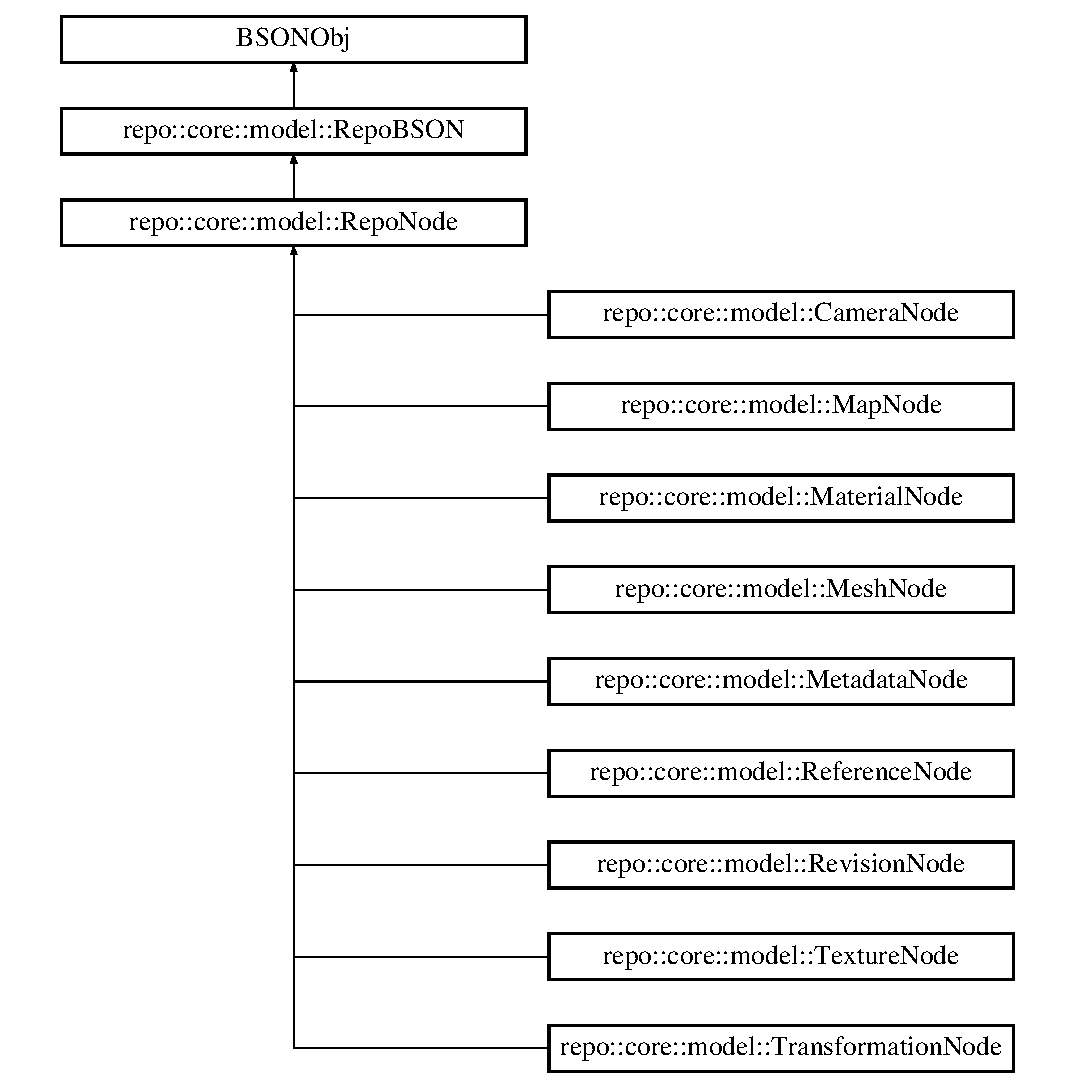
\includegraphics[height=12.000000cm]{classrepo_1_1core_1_1model_1_1_repo_node}
\end{center}
\end{figure}
\subsection*{Public Member Functions}
\begin{DoxyCompactItemize}
\item 
\hyperlink{classrepo_1_1core_1_1model_1_1_repo_node_abec87b9a166ec42041ceced9315acee1}{Repo\+Node} (\hyperlink{classrepo_1_1core_1_1model_1_1_repo_b_s_o_n}{Repo\+B\+S\+O\+N} bson, const std\+::unordered\+\_\+map$<$ std\+::string, std\+::pair$<$ std\+::string, std\+::vector$<$ uint8\+\_\+t $>$$>$$>$ \&bin\+Mapping=std\+::unordered\+\_\+map$<$ std\+::string, std\+::pair$<$ std\+::string, std\+::vector$<$ uint8\+\_\+t $>$$>$$>$())
\item 
\hyperlink{classrepo_1_1core_1_1model_1_1_repo_node_a798034b80fc19d1a83ac60611dad86ea}{Repo\+Node} ()
\item 
virtual \hyperlink{classrepo_1_1core_1_1model_1_1_repo_node_a9d2bfe67f3d2ac044d722bedc5ecdd82}{$\sim$\+Repo\+Node} ()
\item 
virtual bool \hyperlink{classrepo_1_1core_1_1model_1_1_repo_node_aa3e0f98690dc8bfe082d2fc57b904798}{position\+Dependant} ()
\item 
\hyperlink{classrepo_1_1core_1_1model_1_1_repo_node}{Repo\+Node} \hyperlink{classrepo_1_1core_1_1model_1_1_repo_node_abfab119eae3bdc008811dbfe8c2182df}{clone\+And\+Add\+Parent} (const repo\+U\+U\+I\+D \&parent, const bool \&new\+Unique\+I\+D=false, const bool \&new\+Shared\+I\+D=false, const bool \&overwrite=false) const 
\item 
\hyperlink{classrepo_1_1core_1_1model_1_1_repo_node}{Repo\+Node} \hyperlink{classrepo_1_1core_1_1model_1_1_repo_node_afd4ca3df329125f9c1baf654fcdd0b6f}{clone\+And\+Add\+Parent} (const std\+::vector$<$ repo\+U\+U\+I\+D $>$ \&parents) const 
\item 
virtual \hyperlink{classrepo_1_1core_1_1model_1_1_repo_node}{Repo\+Node} \hyperlink{classrepo_1_1core_1_1model_1_1_repo_node_ac31acdb9774bce9296cb5005286db83d}{clone\+And\+Apply\+Transformation} (const std\+::vector$<$ float $>$ \&matrix) const 
\item 
\hyperlink{classrepo_1_1core_1_1model_1_1_repo_node}{Repo\+Node} \hyperlink{classrepo_1_1core_1_1model_1_1_repo_node_a8a6beeff42135007ead59649613df38a}{clone\+And\+Change\+Name} (const std\+::string \&new\+Name, const bool \&new\+Unique\+I\+D=true) const 
\item 
\hyperlink{classrepo_1_1core_1_1model_1_1_repo_node}{Repo\+Node} \hyperlink{classrepo_1_1core_1_1model_1_1_repo_node_ac1b7d9076b255eb4117a6d5a0318fe68}{clone\+And\+Remove\+Parent} (const repo\+U\+U\+I\+D \&parent, const bool \&new\+Unique\+I\+D=true) const 
\item 
virtual \hyperlink{classrepo_1_1core_1_1model_1_1_repo_node}{Repo\+Node} \hyperlink{classrepo_1_1core_1_1model_1_1_repo_node_aed3611c21562e98e2a0d5d715548f496}{clone\+And\+Add\+Fields} (const \hyperlink{classrepo_1_1core_1_1model_1_1_repo_b_s_o_n}{Repo\+B\+S\+O\+N} $\ast$changes, const bool \&new\+Unique\+I\+D=true) const 
\item 
std\+::string \hyperlink{classrepo_1_1core_1_1model_1_1_repo_node_a001c5d809e79efaab4d4949fe466a619}{get\+Name} () const 
\item 
repo\+U\+U\+I\+D \hyperlink{classrepo_1_1core_1_1model_1_1_repo_node_a3d596341d346f03b7a7716ff629b7ce1}{get\+Shared\+I\+D} () const 
\item 
virtual std\+::string \hyperlink{classrepo_1_1core_1_1model_1_1_repo_node_a4380ba349235b5d9b13b41e41975805e}{get\+Type} () const 
\item 
virtual Node\+Type \hyperlink{classrepo_1_1core_1_1model_1_1_repo_node_ad8d5295248dc9beb0b91efb2ce3b61f4}{get\+Type\+As\+Enum} () const 
\item 
repo\+U\+U\+I\+D \hyperlink{classrepo_1_1core_1_1model_1_1_repo_node_aa8a31489284049610e5f472c88a387bd}{get\+Unique\+I\+D} () const 
\item 
std\+::vector$<$ repo\+U\+U\+I\+D $>$ \hyperlink{classrepo_1_1core_1_1model_1_1_repo_node_a20e3664bab40526d592805d910358f09}{get\+Parent\+I\+Ds} () const 
\item 
\hypertarget{classrepo_1_1core_1_1model_1_1_repo_node_aad580ff0ae7dabaef420e52122bf73d6}{}bool \hyperlink{classrepo_1_1core_1_1model_1_1_repo_node_aad580ff0ae7dabaef420e52122bf73d6}{operator==} (const \hyperlink{classrepo_1_1core_1_1model_1_1_repo_node}{Repo\+Node} \&other) const \label{classrepo_1_1core_1_1model_1_1_repo_node_aad580ff0ae7dabaef420e52122bf73d6}

\begin{DoxyCompactList}\small\item\em Returns true if the node is the same, false otherwise. \end{DoxyCompactList}\item 
\hypertarget{classrepo_1_1core_1_1model_1_1_repo_node_a48d57aecd2edd37df9898b75eeda9ca9}{}bool \hyperlink{classrepo_1_1core_1_1model_1_1_repo_node_a48d57aecd2edd37df9898b75eeda9ca9}{operator$<$} (const \hyperlink{classrepo_1_1core_1_1model_1_1_repo_node}{Repo\+Node} \&other) const \label{classrepo_1_1core_1_1model_1_1_repo_node_a48d57aecd2edd37df9898b75eeda9ca9}

\begin{DoxyCompactList}\small\item\em Returns true if the other node is greater than this one, false otherwise. \end{DoxyCompactList}\item 
virtual bool \hyperlink{classrepo_1_1core_1_1model_1_1_repo_node_a7c98830a876ee6516587a8f07c7015a5}{s\+Equal} (const \hyperlink{classrepo_1_1core_1_1model_1_1_repo_node}{Repo\+Node} \&other) const 
\item 
\hypertarget{classrepo_1_1core_1_1model_1_1_repo_node_a79bf797a38615a8a01013f27b82d1075}{}bool \hyperlink{classrepo_1_1core_1_1model_1_1_repo_node_a79bf797a38615a8a01013f27b82d1075}{operator$>$} (const \hyperlink{classrepo_1_1core_1_1model_1_1_repo_node}{Repo\+Node} \&other) const \label{classrepo_1_1core_1_1model_1_1_repo_node_a79bf797a38615a8a01013f27b82d1075}

\begin{DoxyCompactList}\small\item\em Returns true if the other node is greater than this one, false otherwise. \end{DoxyCompactList}\end{DoxyCompactItemize}
\subsection*{Protected Attributes}
\begin{DoxyCompactItemize}
\item 
\hypertarget{classrepo_1_1core_1_1model_1_1_repo_node_a72eab96d654f3f62db12bd7dc3042b7f}{}std\+::string \hyperlink{classrepo_1_1core_1_1model_1_1_repo_node_a72eab96d654f3f62db12bd7dc3042b7f}{type}\label{classrepo_1_1core_1_1model_1_1_repo_node_a72eab96d654f3f62db12bd7dc3042b7f}

\begin{DoxyCompactList}\small\item\em Compulsory type of this document. \end{DoxyCompactList}\end{DoxyCompactItemize}
\subsection*{Additional Inherited Members}


\subsection{Constructor \& Destructor Documentation}
\hypertarget{classrepo_1_1core_1_1model_1_1_repo_node_abec87b9a166ec42041ceced9315acee1}{}\index{repo\+::core\+::model\+::\+Repo\+Node@{repo\+::core\+::model\+::\+Repo\+Node}!Repo\+Node@{Repo\+Node}}
\index{Repo\+Node@{Repo\+Node}!repo\+::core\+::model\+::\+Repo\+Node@{repo\+::core\+::model\+::\+Repo\+Node}}
\subsubsection[{Repo\+Node}]{\setlength{\rightskip}{0pt plus 5cm}Repo\+Node\+::\+Repo\+Node (
\begin{DoxyParamCaption}
\item[{{\bf Repo\+B\+S\+O\+N}}]{bson, }
\item[{const std\+::unordered\+\_\+map$<$ std\+::string, std\+::pair$<$ std\+::string, std\+::vector$<$ uint8\+\_\+t $>$$>$$>$ \&}]{bin\+Mapping = {\ttfamily std\+:\+:unordered\+\_\+map$<$std\+:\+:string,~std\+:\+:pair$<$std\+:\+:string,~std\+:\+:vector$<$uint8\+\_\+t$>$$>$$>$()}}
\end{DoxyParamCaption}
)}\label{classrepo_1_1core_1_1model_1_1_repo_node_abec87b9a166ec42041ceced9315acee1}
Constructor Construct a \hyperlink{classrepo_1_1core_1_1model_1_1_repo_node}{Repo\+Node} base on a \hyperlink{classrepo_1_1core_1_1model_1_1_repo_b_s_o_n}{Repo\+B\+S\+O\+N} object \hypertarget{classrepo_1_1core_1_1model_1_1_repo_node_a798034b80fc19d1a83ac60611dad86ea}{}\index{repo\+::core\+::model\+::\+Repo\+Node@{repo\+::core\+::model\+::\+Repo\+Node}!Repo\+Node@{Repo\+Node}}
\index{Repo\+Node@{Repo\+Node}!repo\+::core\+::model\+::\+Repo\+Node@{repo\+::core\+::model\+::\+Repo\+Node}}
\subsubsection[{Repo\+Node}]{\setlength{\rightskip}{0pt plus 5cm}repo\+::core\+::model\+::\+Repo\+Node\+::\+Repo\+Node (
\begin{DoxyParamCaption}
{}
\end{DoxyParamCaption}
)\hspace{0.3cm}{\ttfamily [inline]}}\label{classrepo_1_1core_1_1model_1_1_repo_node_a798034b80fc19d1a83ac60611dad86ea}
Empty Constructor \hypertarget{classrepo_1_1core_1_1model_1_1_repo_node_a9d2bfe67f3d2ac044d722bedc5ecdd82}{}\index{repo\+::core\+::model\+::\+Repo\+Node@{repo\+::core\+::model\+::\+Repo\+Node}!````~Repo\+Node@{$\sim$\+Repo\+Node}}
\index{````~Repo\+Node@{$\sim$\+Repo\+Node}!repo\+::core\+::model\+::\+Repo\+Node@{repo\+::core\+::model\+::\+Repo\+Node}}
\subsubsection[{$\sim$\+Repo\+Node}]{\setlength{\rightskip}{0pt plus 5cm}Repo\+Node\+::$\sim$\+Repo\+Node (
\begin{DoxyParamCaption}
{}
\end{DoxyParamCaption}
)\hspace{0.3cm}{\ttfamily [virtual]}}\label{classrepo_1_1core_1_1model_1_1_repo_node_a9d2bfe67f3d2ac044d722bedc5ecdd82}
Default Deconstructor 

\subsection{Member Function Documentation}
\hypertarget{classrepo_1_1core_1_1model_1_1_repo_node_aed3611c21562e98e2a0d5d715548f496}{}\index{repo\+::core\+::model\+::\+Repo\+Node@{repo\+::core\+::model\+::\+Repo\+Node}!clone\+And\+Add\+Fields@{clone\+And\+Add\+Fields}}
\index{clone\+And\+Add\+Fields@{clone\+And\+Add\+Fields}!repo\+::core\+::model\+::\+Repo\+Node@{repo\+::core\+::model\+::\+Repo\+Node}}
\subsubsection[{clone\+And\+Add\+Fields}]{\setlength{\rightskip}{0pt plus 5cm}{\bf Repo\+Node} Repo\+Node\+::clone\+And\+Add\+Fields (
\begin{DoxyParamCaption}
\item[{const {\bf Repo\+B\+S\+O\+N} $\ast$}]{changes, }
\item[{const bool \&}]{new\+Unique\+I\+D = {\ttfamily true}}
\end{DoxyParamCaption}
) const\hspace{0.3cm}{\ttfamily [virtual]}}\label{classrepo_1_1core_1_1model_1_1_repo_node_aed3611c21562e98e2a0d5d715548f496}
Create a new object with fields within the change node (excluding parent\+I\+D, unique I\+D and shared I\+D) N\+O\+T\+E this object is unchanged! 
\begin{DoxyParams}{Parameters}
{\em changes} & a repobson containing the fields to change \\
\hline
{\em new\+Unique\+I\+D} & generate a new unique I\+D if set to true \\
\hline
\end{DoxyParams}
\begin{DoxyReturn}{Returns}
returns a new object with fields updated 
\end{DoxyReturn}
\hypertarget{classrepo_1_1core_1_1model_1_1_repo_node_abfab119eae3bdc008811dbfe8c2182df}{}\index{repo\+::core\+::model\+::\+Repo\+Node@{repo\+::core\+::model\+::\+Repo\+Node}!clone\+And\+Add\+Parent@{clone\+And\+Add\+Parent}}
\index{clone\+And\+Add\+Parent@{clone\+And\+Add\+Parent}!repo\+::core\+::model\+::\+Repo\+Node@{repo\+::core\+::model\+::\+Repo\+Node}}
\subsubsection[{clone\+And\+Add\+Parent}]{\setlength{\rightskip}{0pt plus 5cm}{\bf Repo\+Node} Repo\+Node\+::clone\+And\+Add\+Parent (
\begin{DoxyParamCaption}
\item[{const repo\+U\+U\+I\+D \&}]{parent, }
\item[{const bool \&}]{new\+Unique\+I\+D = {\ttfamily false}, }
\item[{const bool \&}]{new\+Shared\+I\+D = {\ttfamily false}, }
\item[{const bool \&}]{overwrite = {\ttfamily false}}
\end{DoxyParamCaption}
) const}\label{classrepo_1_1core_1_1model_1_1_repo_node_abfab119eae3bdc008811dbfe8c2182df}
Create a new object with this object\textquotesingle{}s values, and add another parent into this new object N\+O\+T\+E\+: this object is unchanged! 
\begin{DoxyParams}{Parameters}
{\em parent\+I\+D} & the shared uuid of the parent \\
\hline
{\em new\+Unique\+I\+D} & assign a new unique I\+D \\
\hline
{\em new\+Shared\+I\+D} & assign a new shared I\+D \\
\hline
{\em overwrite} & overwrite the current parenting information \\
\hline
\end{DoxyParams}
\begin{DoxyReturn}{Returns}
new object with the field updated 
\end{DoxyReturn}
\hypertarget{classrepo_1_1core_1_1model_1_1_repo_node_afd4ca3df329125f9c1baf654fcdd0b6f}{}\index{repo\+::core\+::model\+::\+Repo\+Node@{repo\+::core\+::model\+::\+Repo\+Node}!clone\+And\+Add\+Parent@{clone\+And\+Add\+Parent}}
\index{clone\+And\+Add\+Parent@{clone\+And\+Add\+Parent}!repo\+::core\+::model\+::\+Repo\+Node@{repo\+::core\+::model\+::\+Repo\+Node}}
\subsubsection[{clone\+And\+Add\+Parent}]{\setlength{\rightskip}{0pt plus 5cm}{\bf Repo\+Node} Repo\+Node\+::clone\+And\+Add\+Parent (
\begin{DoxyParamCaption}
\item[{const std\+::vector$<$ repo\+U\+U\+I\+D $>$ \&}]{parents}
\end{DoxyParamCaption}
) const}\label{classrepo_1_1core_1_1model_1_1_repo_node_afd4ca3df329125f9c1baf654fcdd0b6f}
Create a new object with this object\textquotesingle{}s values, and add other parents into this new object N\+O\+T\+E\+: this object is unchanged! 
\begin{DoxyParams}{Parameters}
{\em parent\+I\+D} & the shared uuid of the parent \\
\hline
\end{DoxyParams}
\begin{DoxyReturn}{Returns}
new object with the field updated 
\end{DoxyReturn}
\hypertarget{classrepo_1_1core_1_1model_1_1_repo_node_ac31acdb9774bce9296cb5005286db83d}{}\index{repo\+::core\+::model\+::\+Repo\+Node@{repo\+::core\+::model\+::\+Repo\+Node}!clone\+And\+Apply\+Transformation@{clone\+And\+Apply\+Transformation}}
\index{clone\+And\+Apply\+Transformation@{clone\+And\+Apply\+Transformation}!repo\+::core\+::model\+::\+Repo\+Node@{repo\+::core\+::model\+::\+Repo\+Node}}
\subsubsection[{clone\+And\+Apply\+Transformation}]{\setlength{\rightskip}{0pt plus 5cm}virtual {\bf Repo\+Node} repo\+::core\+::model\+::\+Repo\+Node\+::clone\+And\+Apply\+Transformation (
\begin{DoxyParamCaption}
\item[{const std\+::vector$<$ float $>$ \&}]{matrix}
\end{DoxyParamCaption}
) const\hspace{0.3cm}{\ttfamily [inline]}, {\ttfamily [virtual]}}\label{classrepo_1_1core_1_1model_1_1_repo_node_ac31acdb9774bce9296cb5005286db83d}
Create a new object with transformation applied to the node default behaviour is do nothing. Children object needs to override this function to perform their own specific behaviour. 
\begin{DoxyParams}{Parameters}
{\em matrix} & transformation matrix to apply. \\
\hline
\end{DoxyParams}
\begin{DoxyReturn}{Returns}
returns a new object with transformation applied. 
\end{DoxyReturn}


Reimplemented in \hyperlink{classrepo_1_1core_1_1model_1_1_mesh_node_a8f65c14c0c964ee17197135e95e30e3c}{repo\+::core\+::model\+::\+Mesh\+Node}, \hyperlink{classrepo_1_1core_1_1model_1_1_transformation_node_ad7ee2c9234712c2c697e06c02b34ed9b}{repo\+::core\+::model\+::\+Transformation\+Node}, and \hyperlink{classrepo_1_1core_1_1model_1_1_camera_node_a98b1b2260da36fb75ff894c98df901cf}{repo\+::core\+::model\+::\+Camera\+Node}.

\hypertarget{classrepo_1_1core_1_1model_1_1_repo_node_a8a6beeff42135007ead59649613df38a}{}\index{repo\+::core\+::model\+::\+Repo\+Node@{repo\+::core\+::model\+::\+Repo\+Node}!clone\+And\+Change\+Name@{clone\+And\+Change\+Name}}
\index{clone\+And\+Change\+Name@{clone\+And\+Change\+Name}!repo\+::core\+::model\+::\+Repo\+Node@{repo\+::core\+::model\+::\+Repo\+Node}}
\subsubsection[{clone\+And\+Change\+Name}]{\setlength{\rightskip}{0pt plus 5cm}{\bf Repo\+Node} repo\+::core\+::model\+::\+Repo\+Node\+::clone\+And\+Change\+Name (
\begin{DoxyParamCaption}
\item[{const std\+::string \&}]{new\+Name, }
\item[{const bool \&}]{new\+Unique\+I\+D = {\ttfamily true}}
\end{DoxyParamCaption}
) const\hspace{0.3cm}{\ttfamily [inline]}}\label{classrepo_1_1core_1_1model_1_1_repo_node_a8a6beeff42135007ead59649613df38a}
Create a new object with this object\textquotesingle{}s values, but a different name 
\begin{DoxyParams}{Parameters}
{\em new\+Name} & new name \\
\hline
\end{DoxyParams}
\begin{DoxyReturn}{Returns}
returns an object with the change 
\end{DoxyReturn}
\hypertarget{classrepo_1_1core_1_1model_1_1_repo_node_ac1b7d9076b255eb4117a6d5a0318fe68}{}\index{repo\+::core\+::model\+::\+Repo\+Node@{repo\+::core\+::model\+::\+Repo\+Node}!clone\+And\+Remove\+Parent@{clone\+And\+Remove\+Parent}}
\index{clone\+And\+Remove\+Parent@{clone\+And\+Remove\+Parent}!repo\+::core\+::model\+::\+Repo\+Node@{repo\+::core\+::model\+::\+Repo\+Node}}
\subsubsection[{clone\+And\+Remove\+Parent}]{\setlength{\rightskip}{0pt plus 5cm}{\bf Repo\+Node} Repo\+Node\+::clone\+And\+Remove\+Parent (
\begin{DoxyParamCaption}
\item[{const repo\+U\+U\+I\+D \&}]{parent, }
\item[{const bool \&}]{new\+Unique\+I\+D = {\ttfamily true}}
\end{DoxyParamCaption}
) const}\label{classrepo_1_1core_1_1model_1_1_repo_node_ac1b7d9076b255eb4117a6d5a0318fe68}
Create a new object with this object\textquotesingle{}s values, and remove a parent into this new object N\+O\+T\+E\+: this object is unchanged! 
\begin{DoxyParams}{Parameters}
{\em parent\+I\+D} & the shared uuid of the parent \\
\hline
{\em new\+Unique\+I\+D} & generate a new unique I\+D if set to true \\
\hline
\end{DoxyParams}
\begin{DoxyReturn}{Returns}
new object with the field updated 
\end{DoxyReturn}
\hypertarget{classrepo_1_1core_1_1model_1_1_repo_node_a001c5d809e79efaab4d4949fe466a619}{}\index{repo\+::core\+::model\+::\+Repo\+Node@{repo\+::core\+::model\+::\+Repo\+Node}!get\+Name@{get\+Name}}
\index{get\+Name@{get\+Name}!repo\+::core\+::model\+::\+Repo\+Node@{repo\+::core\+::model\+::\+Repo\+Node}}
\subsubsection[{get\+Name}]{\setlength{\rightskip}{0pt plus 5cm}std\+::string repo\+::core\+::model\+::\+Repo\+Node\+::get\+Name (
\begin{DoxyParamCaption}
{}
\end{DoxyParamCaption}
) const\hspace{0.3cm}{\ttfamily [inline]}}\label{classrepo_1_1core_1_1model_1_1_repo_node_a001c5d809e79efaab4d4949fe466a619}
Get the name of the node \begin{DoxyReturn}{Returns}
returns name or \char`\"{}\char`\"{} if no name 
\end{DoxyReturn}
\hypertarget{classrepo_1_1core_1_1model_1_1_repo_node_a20e3664bab40526d592805d910358f09}{}\index{repo\+::core\+::model\+::\+Repo\+Node@{repo\+::core\+::model\+::\+Repo\+Node}!get\+Parent\+I\+Ds@{get\+Parent\+I\+Ds}}
\index{get\+Parent\+I\+Ds@{get\+Parent\+I\+Ds}!repo\+::core\+::model\+::\+Repo\+Node@{repo\+::core\+::model\+::\+Repo\+Node}}
\subsubsection[{get\+Parent\+I\+Ds}]{\setlength{\rightskip}{0pt plus 5cm}std\+::vector$<$ repo\+U\+U\+I\+D $>$ Repo\+Node\+::get\+Parent\+I\+Ds (
\begin{DoxyParamCaption}
{}
\end{DoxyParamCaption}
) const}\label{classrepo_1_1core_1_1model_1_1_repo_node_a20e3664bab40526d592805d910358f09}
Get the list of parent I\+Ds \begin{DoxyReturn}{Returns}
returns a set of parent I\+Ds 
\end{DoxyReturn}
\hypertarget{classrepo_1_1core_1_1model_1_1_repo_node_a3d596341d346f03b7a7716ff629b7ce1}{}\index{repo\+::core\+::model\+::\+Repo\+Node@{repo\+::core\+::model\+::\+Repo\+Node}!get\+Shared\+I\+D@{get\+Shared\+I\+D}}
\index{get\+Shared\+I\+D@{get\+Shared\+I\+D}!repo\+::core\+::model\+::\+Repo\+Node@{repo\+::core\+::model\+::\+Repo\+Node}}
\subsubsection[{get\+Shared\+I\+D}]{\setlength{\rightskip}{0pt plus 5cm}repo\+U\+U\+I\+D repo\+::core\+::model\+::\+Repo\+Node\+::get\+Shared\+I\+D (
\begin{DoxyParamCaption}
{}
\end{DoxyParamCaption}
) const\hspace{0.3cm}{\ttfamily [inline]}}\label{classrepo_1_1core_1_1model_1_1_repo_node_a3d596341d346f03b7a7716ff629b7ce1}
Get the shared I\+D from the object \begin{DoxyReturn}{Returns}
returns the shared I\+D of the object 
\end{DoxyReturn}
\hypertarget{classrepo_1_1core_1_1model_1_1_repo_node_a4380ba349235b5d9b13b41e41975805e}{}\index{repo\+::core\+::model\+::\+Repo\+Node@{repo\+::core\+::model\+::\+Repo\+Node}!get\+Type@{get\+Type}}
\index{get\+Type@{get\+Type}!repo\+::core\+::model\+::\+Repo\+Node@{repo\+::core\+::model\+::\+Repo\+Node}}
\subsubsection[{get\+Type}]{\setlength{\rightskip}{0pt plus 5cm}virtual std\+::string repo\+::core\+::model\+::\+Repo\+Node\+::get\+Type (
\begin{DoxyParamCaption}
{}
\end{DoxyParamCaption}
) const\hspace{0.3cm}{\ttfamily [inline]}, {\ttfamily [virtual]}}\label{classrepo_1_1core_1_1model_1_1_repo_node_a4380ba349235b5d9b13b41e41975805e}
Get the type of node \begin{DoxyReturn}{Returns}
returns the type as a string 
\end{DoxyReturn}


Reimplemented in \hyperlink{classrepo_1_1core_1_1model_1_1_mesh_node_afb8fedac41e86bce0f74509efa6d9614}{repo\+::core\+::model\+::\+Mesh\+Node}, \hyperlink{classrepo_1_1core_1_1model_1_1_transformation_node_a7e0b577dccbdbcab1e833b4da3121e83}{repo\+::core\+::model\+::\+Transformation\+Node}, \hyperlink{classrepo_1_1core_1_1model_1_1_revision_node_ac597aa317c2516be9f204e43ef896af4}{repo\+::core\+::model\+::\+Revision\+Node}, \hyperlink{classrepo_1_1core_1_1model_1_1_material_node_af0debb10133049af18a7c1e45942b606}{repo\+::core\+::model\+::\+Material\+Node}, \hyperlink{classrepo_1_1core_1_1model_1_1_reference_node_a1f1b1c966eb936b31b92f05247df58d0}{repo\+::core\+::model\+::\+Reference\+Node}, \hyperlink{classrepo_1_1core_1_1model_1_1_texture_node_aaae4c87e4e841d8bddc105e29e759d2a}{repo\+::core\+::model\+::\+Texture\+Node}, and \hyperlink{classrepo_1_1core_1_1model_1_1_metadata_node_aad51dc79d63495aa6b4b8fd02307786f}{repo\+::core\+::model\+::\+Metadata\+Node}.

\hypertarget{classrepo_1_1core_1_1model_1_1_repo_node_ad8d5295248dc9beb0b91efb2ce3b61f4}{}\index{repo\+::core\+::model\+::\+Repo\+Node@{repo\+::core\+::model\+::\+Repo\+Node}!get\+Type\+As\+Enum@{get\+Type\+As\+Enum}}
\index{get\+Type\+As\+Enum@{get\+Type\+As\+Enum}!repo\+::core\+::model\+::\+Repo\+Node@{repo\+::core\+::model\+::\+Repo\+Node}}
\subsubsection[{get\+Type\+As\+Enum}]{\setlength{\rightskip}{0pt plus 5cm}Node\+Type Repo\+Node\+::get\+Type\+As\+Enum (
\begin{DoxyParamCaption}
{}
\end{DoxyParamCaption}
) const\hspace{0.3cm}{\ttfamily [virtual]}}\label{classrepo_1_1core_1_1model_1_1_repo_node_ad8d5295248dc9beb0b91efb2ce3b61f4}
Get the type of node as an enum \begin{DoxyReturn}{Returns}
returns type as enum. 
\end{DoxyReturn}


Reimplemented in \hyperlink{classrepo_1_1core_1_1model_1_1_mesh_node_aba656559a131b00514ca844a7e8a595c}{repo\+::core\+::model\+::\+Mesh\+Node}, \hyperlink{classrepo_1_1core_1_1model_1_1_transformation_node_ae24b2692960c32fed8b8b1ebf732a333}{repo\+::core\+::model\+::\+Transformation\+Node}, \hyperlink{classrepo_1_1core_1_1model_1_1_revision_node_ae632d941e5a9bc2d8275c53bb1c41805}{repo\+::core\+::model\+::\+Revision\+Node}, \hyperlink{classrepo_1_1core_1_1model_1_1_material_node_aa971c1eb43b76f95f28c063dac9919bc}{repo\+::core\+::model\+::\+Material\+Node}, \hyperlink{classrepo_1_1core_1_1model_1_1_reference_node_abe69afbcb44f14ad6a9a821819a2cf85}{repo\+::core\+::model\+::\+Reference\+Node}, \hyperlink{classrepo_1_1core_1_1model_1_1_texture_node_a78fadf9b11659cf83c24d367b66a6772}{repo\+::core\+::model\+::\+Texture\+Node}, and \hyperlink{classrepo_1_1core_1_1model_1_1_metadata_node_abc913943e7ce90649aa0d94ef70552ce}{repo\+::core\+::model\+::\+Metadata\+Node}.

\hypertarget{classrepo_1_1core_1_1model_1_1_repo_node_aa8a31489284049610e5f472c88a387bd}{}\index{repo\+::core\+::model\+::\+Repo\+Node@{repo\+::core\+::model\+::\+Repo\+Node}!get\+Unique\+I\+D@{get\+Unique\+I\+D}}
\index{get\+Unique\+I\+D@{get\+Unique\+I\+D}!repo\+::core\+::model\+::\+Repo\+Node@{repo\+::core\+::model\+::\+Repo\+Node}}
\subsubsection[{get\+Unique\+I\+D}]{\setlength{\rightskip}{0pt plus 5cm}repo\+U\+U\+I\+D repo\+::core\+::model\+::\+Repo\+Node\+::get\+Unique\+I\+D (
\begin{DoxyParamCaption}
{}
\end{DoxyParamCaption}
) const\hspace{0.3cm}{\ttfamily [inline]}}\label{classrepo_1_1core_1_1model_1_1_repo_node_aa8a31489284049610e5f472c88a387bd}
Get the unique I\+D from the object \begin{DoxyReturn}{Returns}
returns the unique I\+D of the object 
\end{DoxyReturn}
\hypertarget{classrepo_1_1core_1_1model_1_1_repo_node_aa3e0f98690dc8bfe082d2fc57b904798}{}\index{repo\+::core\+::model\+::\+Repo\+Node@{repo\+::core\+::model\+::\+Repo\+Node}!position\+Dependant@{position\+Dependant}}
\index{position\+Dependant@{position\+Dependant}!repo\+::core\+::model\+::\+Repo\+Node@{repo\+::core\+::model\+::\+Repo\+Node}}
\subsubsection[{position\+Dependant}]{\setlength{\rightskip}{0pt plus 5cm}virtual bool repo\+::core\+::model\+::\+Repo\+Node\+::position\+Dependant (
\begin{DoxyParamCaption}
{}
\end{DoxyParamCaption}
)\hspace{0.3cm}{\ttfamily [inline]}, {\ttfamily [virtual]}}\label{classrepo_1_1core_1_1model_1_1_repo_node_aa3e0f98690dc8bfe082d2fc57b904798}
Check if the node is position dependant. i.\+e. if parent transformation is merged onto the node, does the node requre to a transformation applied to it e.\+g. meshes and cameras are position dependant, metadata isn\textquotesingle{}t Default behaviour is false. Position dependant child requires override this function. \begin{DoxyReturn}{Returns}
true if node is position\+Dependant. 
\end{DoxyReturn}


Reimplemented in \hyperlink{classrepo_1_1core_1_1model_1_1_mesh_node_a636fc543dbbeca60698e8719c11f945d}{repo\+::core\+::model\+::\+Mesh\+Node}, \hyperlink{classrepo_1_1core_1_1model_1_1_transformation_node_aef0c61c652ac425139a063c5e5c1832b}{repo\+::core\+::model\+::\+Transformation\+Node}, and \hyperlink{classrepo_1_1core_1_1model_1_1_camera_node_a5ff50e052f4266842e5d4e4840fe0c37}{repo\+::core\+::model\+::\+Camera\+Node}.

\hypertarget{classrepo_1_1core_1_1model_1_1_repo_node_a7c98830a876ee6516587a8f07c7015a5}{}\index{repo\+::core\+::model\+::\+Repo\+Node@{repo\+::core\+::model\+::\+Repo\+Node}!s\+Equal@{s\+Equal}}
\index{s\+Equal@{s\+Equal}!repo\+::core\+::model\+::\+Repo\+Node@{repo\+::core\+::model\+::\+Repo\+Node}}
\subsubsection[{s\+Equal}]{\setlength{\rightskip}{0pt plus 5cm}virtual bool repo\+::core\+::model\+::\+Repo\+Node\+::s\+Equal (
\begin{DoxyParamCaption}
\item[{const {\bf Repo\+Node} \&}]{other}
\end{DoxyParamCaption}
) const\hspace{0.3cm}{\ttfamily [inline]}, {\ttfamily [virtual]}}\label{classrepo_1_1core_1_1model_1_1_repo_node_a7c98830a876ee6516587a8f07c7015a5}
Check if the node is semantically equal to another Different node should have a different interpretation of what this means. 
\begin{DoxyParams}{Parameters}
{\em other} & node to compare with \\
\hline
{\em returns} & true if equal, false otherwise \\
\hline
\end{DoxyParams}


Reimplemented in \hyperlink{classrepo_1_1core_1_1model_1_1_camera_node_a4d4a8875d7929aa92beedd9bd0eeea63}{repo\+::core\+::model\+::\+Camera\+Node}, \hyperlink{classrepo_1_1core_1_1model_1_1_map_node_ac27593deef8281f9d70324f2f1f994e9}{repo\+::core\+::model\+::\+Map\+Node}, \hyperlink{classrepo_1_1core_1_1model_1_1_mesh_node_a58dbc8bb0cdcbbae2e0c6e7558eaef70}{repo\+::core\+::model\+::\+Mesh\+Node}, \hyperlink{classrepo_1_1core_1_1model_1_1_transformation_node_ae580f6d1f6e6d331180ab6bb408f7e66}{repo\+::core\+::model\+::\+Transformation\+Node}, \hyperlink{classrepo_1_1core_1_1model_1_1_material_node_a65fe37720ba763de81789f5c4f66039a}{repo\+::core\+::model\+::\+Material\+Node}, \hyperlink{classrepo_1_1core_1_1model_1_1_reference_node_abc948b4ed5437871142d57498a12cf2d}{repo\+::core\+::model\+::\+Reference\+Node}, \hyperlink{classrepo_1_1core_1_1model_1_1_texture_node_acc560eb9f51e63bb83d35e859ee4f4c4}{repo\+::core\+::model\+::\+Texture\+Node}, and \hyperlink{classrepo_1_1core_1_1model_1_1_metadata_node_a1fd8134ef9585578597b4a8145aebe1d}{repo\+::core\+::model\+::\+Metadata\+Node}.



The documentation for this class was generated from the following files\+:\begin{DoxyCompactItemize}
\item 
C\+:/\+Users/\+Carmen/3\+D Repo/\+Repo/3drepobouncer/bouncer/src/repo/core/model/bson/repo\+\_\+node.\+h\item 
C\+:/\+Users/\+Carmen/3\+D Repo/\+Repo/3drepobouncer/bouncer/src/repo/core/model/bson/repo\+\_\+node.\+cpp\end{DoxyCompactItemize}

\hypertarget{structrepo_1_1core_1_1model_1_1_repo_node_comparator}{}\section{repo\+:\+:core\+:\+:model\+:\+:Repo\+Node\+Comparator Struct Reference}
\label{structrepo_1_1core_1_1model_1_1_repo_node_comparator}\index{repo\+::core\+::model\+::\+Repo\+Node\+Comparator@{repo\+::core\+::model\+::\+Repo\+Node\+Comparator}}


{\ttfamily \#include $<$repo\+\_\+node.\+h$>$}

\subsection*{Public Member Functions}
\begin{DoxyCompactItemize}
\item 
\hypertarget{structrepo_1_1core_1_1model_1_1_repo_node_comparator_aee57da2f03675e596c08eaa2fe3c1c93}{}bool {\bfseries operator()} (const \hyperlink{classrepo_1_1core_1_1model_1_1_repo_node}{Repo\+Node} $\ast$a, const \hyperlink{classrepo_1_1core_1_1model_1_1_repo_node}{Repo\+Node} $\ast$b) const \label{structrepo_1_1core_1_1model_1_1_repo_node_comparator_aee57da2f03675e596c08eaa2fe3c1c93}

\end{DoxyCompactItemize}


\subsection{Detailed Description}
Comparator definition to enable std\+::set to store pointers to abstract nodes so that they are compared based on their value rather than their integer pointers.

This is a general Repo Node comparator where you would expect a different shared I\+D and unique I\+D. Should a different comparator is needed it should be implemented on that node\textquotesingle{}s class level 

The documentation for this struct was generated from the following file\+:\begin{DoxyCompactItemize}
\item 
C\+:/\+Users/\+Carmen/3\+D Repo/\+Repo/3drepobouncer/bouncer/src/repo/core/model/bson/repo\+\_\+node.\+h\end{DoxyCompactItemize}

\hypertarget{structrepo_1_1core_1_1model_1_1_repo_permission}{}\section{repo\+:\+:core\+:\+:model\+:\+:Repo\+Permission Struct Reference}
\label{structrepo_1_1core_1_1model_1_1_repo_permission}\index{repo\+::core\+::model\+::\+Repo\+Permission@{repo\+::core\+::model\+::\+Repo\+Permission}}
\subsection*{Public Attributes}
\begin{DoxyCompactItemize}
\item 
\hypertarget{structrepo_1_1core_1_1model_1_1_repo_permission_a729698f5134e17dda782c02ba04c4aa2}{}std\+::string {\bfseries database}\label{structrepo_1_1core_1_1model_1_1_repo_permission_a729698f5134e17dda782c02ba04c4aa2}

\item 
\hypertarget{structrepo_1_1core_1_1model_1_1_repo_permission_acedc7f109b755dc5c8f0ff1cd434ed8f}{}std\+::string {\bfseries project}\label{structrepo_1_1core_1_1model_1_1_repo_permission_acedc7f109b755dc5c8f0ff1cd434ed8f}

\item 
\hypertarget{structrepo_1_1core_1_1model_1_1_repo_permission_aacf4a9896fe2dfc690ebea4037da07f9}{}Access\+Right {\bfseries permission}\label{structrepo_1_1core_1_1model_1_1_repo_permission_aacf4a9896fe2dfc690ebea4037da07f9}

\end{DoxyCompactItemize}


The documentation for this struct was generated from the following file\+:\begin{DoxyCompactItemize}
\item 
C\+:/\+Users/\+Carmen/3\+D Repo/\+Repo/3drepobouncer/bouncer/src/repo/core/model/bson/repo\+\_\+bson\+\_\+role.\+h\end{DoxyCompactItemize}

\hypertarget{structrepo_1_1core_1_1model_1_1_repo_privilege}{}\section{repo\+:\+:core\+:\+:model\+:\+:Repo\+Privilege Struct Reference}
\label{structrepo_1_1core_1_1model_1_1_repo_privilege}\index{repo\+::core\+::model\+::\+Repo\+Privilege@{repo\+::core\+::model\+::\+Repo\+Privilege}}
\subsection*{Public Attributes}
\begin{DoxyCompactItemize}
\item 
\hypertarget{structrepo_1_1core_1_1model_1_1_repo_privilege_ae66e9b0f4e6277846c3bb595a2aeac94}{}std\+::string {\bfseries database}\label{structrepo_1_1core_1_1model_1_1_repo_privilege_ae66e9b0f4e6277846c3bb595a2aeac94}

\item 
\hypertarget{structrepo_1_1core_1_1model_1_1_repo_privilege_a3204de8ddd535e806a88f534babe7b16}{}std\+::string {\bfseries collection}\label{structrepo_1_1core_1_1model_1_1_repo_privilege_a3204de8ddd535e806a88f534babe7b16}

\item 
\hypertarget{structrepo_1_1core_1_1model_1_1_repo_privilege_ab9d0732f23ce39feb5d9c02b27703e1a}{}std\+::vector$<$ D\+B\+Actions $>$ {\bfseries actions}\label{structrepo_1_1core_1_1model_1_1_repo_privilege_ab9d0732f23ce39feb5d9c02b27703e1a}

\end{DoxyCompactItemize}


The documentation for this struct was generated from the following file\+:\begin{DoxyCompactItemize}
\item 
C\+:/\+Users/\+Carmen/3\+D Repo/\+Repo/3drepobouncer/bouncer/src/repo/core/model/bson/repo\+\_\+bson\+\_\+role.\+h\end{DoxyCompactItemize}

\hypertarget{classrepo_1_1core_1_1model_1_1_repo_project_settings}{}\section{repo\+:\+:core\+:\+:model\+:\+:Repo\+Project\+Settings Class Reference}
\label{classrepo_1_1core_1_1model_1_1_repo_project_settings}\index{repo\+::core\+::model\+::\+Repo\+Project\+Settings@{repo\+::core\+::model\+::\+Repo\+Project\+Settings}}
Inheritance diagram for repo\+:\+:core\+:\+:model\+:\+:Repo\+Project\+Settings\+:\begin{figure}[H]
\begin{center}
\leavevmode
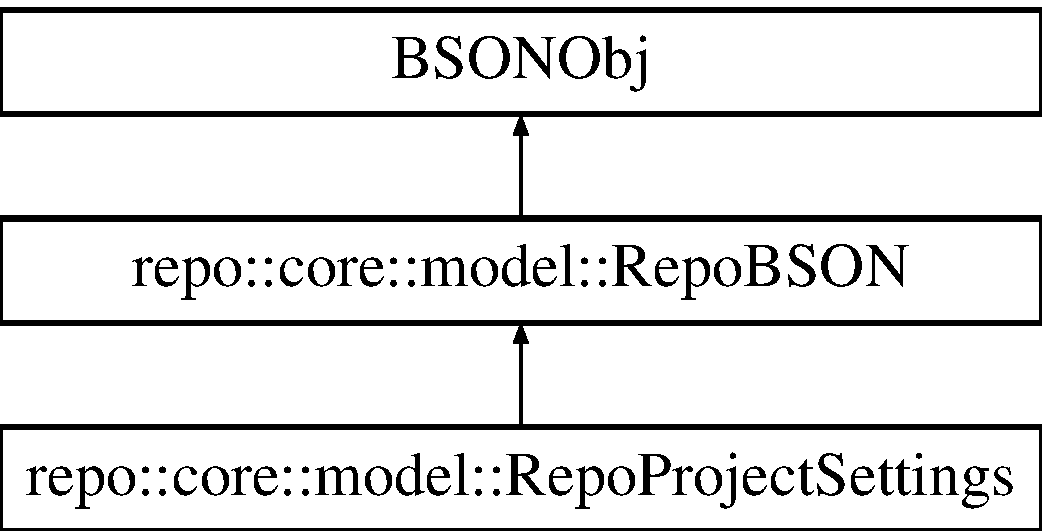
\includegraphics[height=3.000000cm]{classrepo_1_1core_1_1model_1_1_repo_project_settings}
\end{center}
\end{figure}
\subsection*{Public Member Functions}
\begin{DoxyCompactItemize}
\item 
\hypertarget{classrepo_1_1core_1_1model_1_1_repo_project_settings_a1d6a75f7862fbc59f93e29970dc04a58}{}{\bfseries Repo\+Project\+Settings} (\hyperlink{classrepo_1_1core_1_1model_1_1_repo_b_s_o_n}{Repo\+B\+S\+O\+N} bson)\label{classrepo_1_1core_1_1model_1_1_repo_project_settings_a1d6a75f7862fbc59f93e29970dc04a58}

\item 
\hyperlink{classrepo_1_1core_1_1model_1_1_repo_project_settings}{Repo\+Project\+Settings} \hyperlink{classrepo_1_1core_1_1model_1_1_repo_project_settings_a8b06243dafac7759d776c62b21d84516}{clone\+And\+Merge\+Project\+Settings} (const \hyperlink{classrepo_1_1core_1_1model_1_1_repo_project_settings}{Repo\+Project\+Settings} \&proj) const 
\item 
double \hyperlink{classrepo_1_1core_1_1model_1_1_repo_project_settings_af0bc7f83f4a7cfe072684ba524016060}{get\+Avatar\+Height} () const 
\begin{DoxyCompactList}\small\item\em get\+Avatar\+Height \end{DoxyCompactList}\item 
std\+::string \hyperlink{classrepo_1_1core_1_1model_1_1_repo_project_settings_a38501a07d34deb1b79e2bbf82f1cd0c2}{get\+Description} () const 
\item 
std\+::string \hyperlink{classrepo_1_1core_1_1model_1_1_repo_project_settings_a913555bb08814a0a6d19468f06135167}{get\+Owner} () const 
\item 
\hypertarget{classrepo_1_1core_1_1model_1_1_repo_project_settings_a346e97eeca7e2240636d38c6c782dc84}{}double {\bfseries get\+Pin\+Size} () const \label{classrepo_1_1core_1_1model_1_1_repo_project_settings_a346e97eeca7e2240636d38c6c782dc84}

\item 
std\+::string \hyperlink{classrepo_1_1core_1_1model_1_1_repo_project_settings_a4eb1f1aef8f2bd7b92bd0e01e8602731}{get\+Project\+Name} () const 
\item 
\hypertarget{classrepo_1_1core_1_1model_1_1_repo_project_settings_ababb3684d12b3a9ad43a2fa066409a7e}{}double {\bfseries get\+Speed} () const \label{classrepo_1_1core_1_1model_1_1_repo_project_settings_ababb3684d12b3a9ad43a2fa066409a7e}

\item 
std\+::string \hyperlink{classrepo_1_1core_1_1model_1_1_repo_project_settings_a9a3201cc11987611615084705bf5df1e}{get\+Type} () const 
\item 
\hypertarget{classrepo_1_1core_1_1model_1_1_repo_project_settings_aee4450b3159532e78a4a5fdacea4ddcf}{}double {\bfseries get\+Visibility\+Limit} () const \label{classrepo_1_1core_1_1model_1_1_repo_project_settings_aee4450b3159532e78a4a5fdacea4ddcf}

\item 
\hypertarget{classrepo_1_1core_1_1model_1_1_repo_project_settings_ae8e7894c07bdc4fce627c4f76613b960}{}double {\bfseries get\+Z\+Far} () const \label{classrepo_1_1core_1_1model_1_1_repo_project_settings_ae8e7894c07bdc4fce627c4f76613b960}

\item 
double \hyperlink{classrepo_1_1core_1_1model_1_1_repo_project_settings_a9f448ea11943162bfc3f5a05f6edee44}{get\+Z\+Near} () const 
\end{DoxyCompactItemize}
\subsection*{Additional Inherited Members}


\subsection{Member Function Documentation}
\hypertarget{classrepo_1_1core_1_1model_1_1_repo_project_settings_a8b06243dafac7759d776c62b21d84516}{}\index{repo\+::core\+::model\+::\+Repo\+Project\+Settings@{repo\+::core\+::model\+::\+Repo\+Project\+Settings}!clone\+And\+Merge\+Project\+Settings@{clone\+And\+Merge\+Project\+Settings}}
\index{clone\+And\+Merge\+Project\+Settings@{clone\+And\+Merge\+Project\+Settings}!repo\+::core\+::model\+::\+Repo\+Project\+Settings@{repo\+::core\+::model\+::\+Repo\+Project\+Settings}}
\subsubsection[{clone\+And\+Merge\+Project\+Settings}]{\setlength{\rightskip}{0pt plus 5cm}{\bf Repo\+Project\+Settings} Repo\+Project\+Settings\+::clone\+And\+Merge\+Project\+Settings (
\begin{DoxyParamCaption}
\item[{const {\bf Repo\+Project\+Settings} \&}]{proj}
\end{DoxyParamCaption}
) const}\label{classrepo_1_1core_1_1model_1_1_repo_project_settings_a8b06243dafac7759d776c62b21d84516}
Clone and merge new project settings into the existing info  new info that needs ot be added/updated \begin{DoxyReturn}{Returns}
returns a new project settings with fields updated 
\end{DoxyReturn}
\hypertarget{classrepo_1_1core_1_1model_1_1_repo_project_settings_af0bc7f83f4a7cfe072684ba524016060}{}\index{repo\+::core\+::model\+::\+Repo\+Project\+Settings@{repo\+::core\+::model\+::\+Repo\+Project\+Settings}!get\+Avatar\+Height@{get\+Avatar\+Height}}
\index{get\+Avatar\+Height@{get\+Avatar\+Height}!repo\+::core\+::model\+::\+Repo\+Project\+Settings@{repo\+::core\+::model\+::\+Repo\+Project\+Settings}}
\subsubsection[{get\+Avatar\+Height}]{\setlength{\rightskip}{0pt plus 5cm}double repo\+::core\+::model\+::\+Repo\+Project\+Settings\+::get\+Avatar\+Height (
\begin{DoxyParamCaption}
{}
\end{DoxyParamCaption}
) const\hspace{0.3cm}{\ttfamily [inline]}}\label{classrepo_1_1core_1_1model_1_1_repo_project_settings_af0bc7f83f4a7cfe072684ba524016060}


get\+Avatar\+Height 

Get the avatar height if present or default value if not. \begin{DoxyReturn}{Returns}
returns avatar height as double. 
\end{DoxyReturn}
\hypertarget{classrepo_1_1core_1_1model_1_1_repo_project_settings_a38501a07d34deb1b79e2bbf82f1cd0c2}{}\index{repo\+::core\+::model\+::\+Repo\+Project\+Settings@{repo\+::core\+::model\+::\+Repo\+Project\+Settings}!get\+Description@{get\+Description}}
\index{get\+Description@{get\+Description}!repo\+::core\+::model\+::\+Repo\+Project\+Settings@{repo\+::core\+::model\+::\+Repo\+Project\+Settings}}
\subsubsection[{get\+Description}]{\setlength{\rightskip}{0pt plus 5cm}std\+::string repo\+::core\+::model\+::\+Repo\+Project\+Settings\+::get\+Description (
\begin{DoxyParamCaption}
{}
\end{DoxyParamCaption}
) const\hspace{0.3cm}{\ttfamily [inline]}}\label{classrepo_1_1core_1_1model_1_1_repo_project_settings_a38501a07d34deb1b79e2bbf82f1cd0c2}
Get the description of the project for this settings \begin{DoxyReturn}{Returns}
returns project description as string 
\end{DoxyReturn}
\hypertarget{classrepo_1_1core_1_1model_1_1_repo_project_settings_a913555bb08814a0a6d19468f06135167}{}\index{repo\+::core\+::model\+::\+Repo\+Project\+Settings@{repo\+::core\+::model\+::\+Repo\+Project\+Settings}!get\+Owner@{get\+Owner}}
\index{get\+Owner@{get\+Owner}!repo\+::core\+::model\+::\+Repo\+Project\+Settings@{repo\+::core\+::model\+::\+Repo\+Project\+Settings}}
\subsubsection[{get\+Owner}]{\setlength{\rightskip}{0pt plus 5cm}std\+::string repo\+::core\+::model\+::\+Repo\+Project\+Settings\+::get\+Owner (
\begin{DoxyParamCaption}
{}
\end{DoxyParamCaption}
) const\hspace{0.3cm}{\ttfamily [inline]}}\label{classrepo_1_1core_1_1model_1_1_repo_project_settings_a913555bb08814a0a6d19468f06135167}
Get the owner of the project for this settings \begin{DoxyReturn}{Returns}
returns owner name as string 
\end{DoxyReturn}
\hypertarget{classrepo_1_1core_1_1model_1_1_repo_project_settings_a4eb1f1aef8f2bd7b92bd0e01e8602731}{}\index{repo\+::core\+::model\+::\+Repo\+Project\+Settings@{repo\+::core\+::model\+::\+Repo\+Project\+Settings}!get\+Project\+Name@{get\+Project\+Name}}
\index{get\+Project\+Name@{get\+Project\+Name}!repo\+::core\+::model\+::\+Repo\+Project\+Settings@{repo\+::core\+::model\+::\+Repo\+Project\+Settings}}
\subsubsection[{get\+Project\+Name}]{\setlength{\rightskip}{0pt plus 5cm}std\+::string repo\+::core\+::model\+::\+Repo\+Project\+Settings\+::get\+Project\+Name (
\begin{DoxyParamCaption}
{}
\end{DoxyParamCaption}
) const\hspace{0.3cm}{\ttfamily [inline]}}\label{classrepo_1_1core_1_1model_1_1_repo_project_settings_a4eb1f1aef8f2bd7b92bd0e01e8602731}
Get the name of the project for this settings \begin{DoxyReturn}{Returns}
returns project name as string 
\end{DoxyReturn}
\hypertarget{classrepo_1_1core_1_1model_1_1_repo_project_settings_a9a3201cc11987611615084705bf5df1e}{}\index{repo\+::core\+::model\+::\+Repo\+Project\+Settings@{repo\+::core\+::model\+::\+Repo\+Project\+Settings}!get\+Type@{get\+Type}}
\index{get\+Type@{get\+Type}!repo\+::core\+::model\+::\+Repo\+Project\+Settings@{repo\+::core\+::model\+::\+Repo\+Project\+Settings}}
\subsubsection[{get\+Type}]{\setlength{\rightskip}{0pt plus 5cm}std\+::string repo\+::core\+::model\+::\+Repo\+Project\+Settings\+::get\+Type (
\begin{DoxyParamCaption}
{}
\end{DoxyParamCaption}
) const\hspace{0.3cm}{\ttfamily [inline]}}\label{classrepo_1_1core_1_1model_1_1_repo_project_settings_a9a3201cc11987611615084705bf5df1e}
Get the type of the project for this settings \begin{DoxyReturn}{Returns}
returns project type as string 
\end{DoxyReturn}
\hypertarget{classrepo_1_1core_1_1model_1_1_repo_project_settings_a9f448ea11943162bfc3f5a05f6edee44}{}\index{repo\+::core\+::model\+::\+Repo\+Project\+Settings@{repo\+::core\+::model\+::\+Repo\+Project\+Settings}!get\+Z\+Near@{get\+Z\+Near}}
\index{get\+Z\+Near@{get\+Z\+Near}!repo\+::core\+::model\+::\+Repo\+Project\+Settings@{repo\+::core\+::model\+::\+Repo\+Project\+Settings}}
\subsubsection[{get\+Z\+Near}]{\setlength{\rightskip}{0pt plus 5cm}double repo\+::core\+::model\+::\+Repo\+Project\+Settings\+::get\+Z\+Near (
\begin{DoxyParamCaption}
{}
\end{DoxyParamCaption}
) const\hspace{0.3cm}{\ttfamily [inline]}}\label{classrepo_1_1core_1_1model_1_1_repo_project_settings_a9f448ea11943162bfc3f5a05f6edee44}
Get the z\+Near of the project for this settings \begin{DoxyReturn}{Returns}
returns project z\+Near as double 
\end{DoxyReturn}


The documentation for this class was generated from the following files\+:\begin{DoxyCompactItemize}
\item 
C\+:/\+Users/\+Carmen/3\+D Repo/\+Repo/3drepobouncer/bouncer/src/repo/core/model/bson/repo\+\_\+bson\+\_\+project\+\_\+settings.\+h\item 
C\+:/\+Users/\+Carmen/3\+D Repo/\+Repo/3drepobouncer/bouncer/src/repo/core/model/bson/repo\+\_\+bson\+\_\+project\+\_\+settings.\+cpp\end{DoxyCompactItemize}

\hypertarget{classrepo_1_1core_1_1model_1_1_repo_role}{}\section{repo\+:\+:core\+:\+:model\+:\+:Repo\+Role Class Reference}
\label{classrepo_1_1core_1_1model_1_1_repo_role}\index{repo\+::core\+::model\+::\+Repo\+Role@{repo\+::core\+::model\+::\+Repo\+Role}}
Inheritance diagram for repo\+:\+:core\+:\+:model\+:\+:Repo\+Role\+:\begin{figure}[H]
\begin{center}
\leavevmode
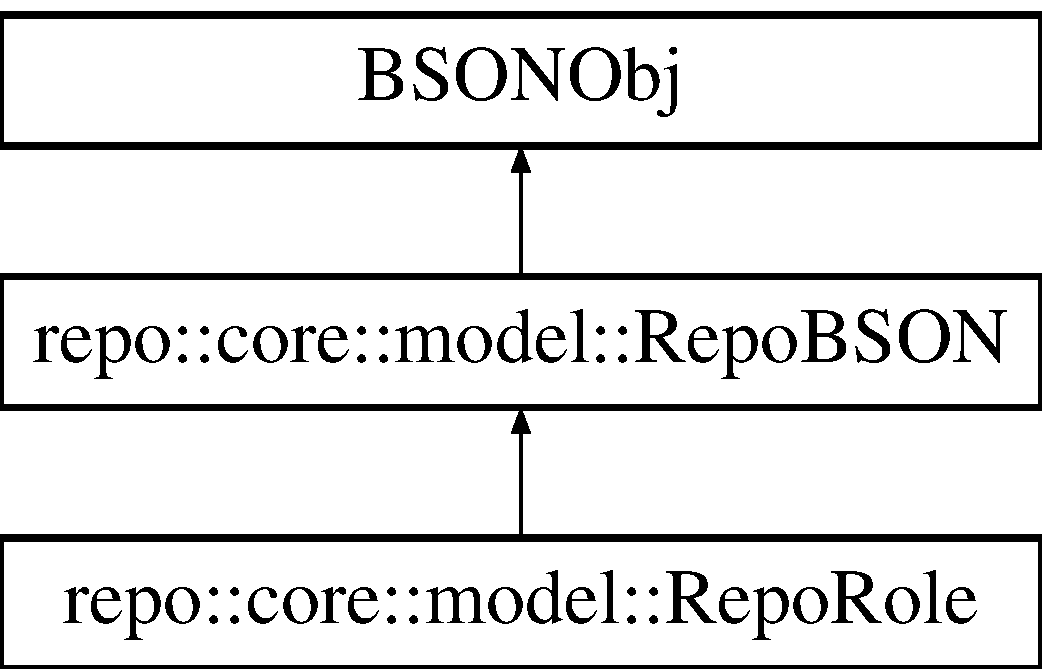
\includegraphics[height=3.000000cm]{classrepo_1_1core_1_1model_1_1_repo_role}
\end{center}
\end{figure}
\subsection*{Public Member Functions}
\begin{DoxyCompactItemize}
\item 
\hypertarget{classrepo_1_1core_1_1model_1_1_repo_role_af9ddc044e897b262065504697e87d756}{}{\bfseries Repo\+Role} (\hyperlink{classrepo_1_1core_1_1model_1_1_repo_b_s_o_n}{Repo\+B\+S\+O\+N} bson)\label{classrepo_1_1core_1_1model_1_1_repo_role_af9ddc044e897b262065504697e87d756}

\item 
\hyperlink{classrepo_1_1core_1_1model_1_1_repo_role}{Repo\+Role} \hyperlink{classrepo_1_1core_1_1model_1_1_repo_role_abdb1f705fc8aa347ffdfbb382fa36160}{clone\+And\+Update\+Permissions} (const std\+::vector$<$ \hyperlink{structrepo_1_1core_1_1model_1_1_repo_permission}{Repo\+Permission} $>$ \&permissions) const 
\item 
\hyperlink{classrepo_1_1core_1_1model_1_1_repo_role}{Repo\+Role} \hyperlink{classrepo_1_1core_1_1model_1_1_repo_role_ac4e6810785f991ba81a93303237755b8}{clone\+And\+Update\+Privileges} (const std\+::vector$<$ \hyperlink{structrepo_1_1core_1_1model_1_1_repo_privilege}{Repo\+Privilege} $>$ \&privileges) const 
\item 
std\+::string \hyperlink{classrepo_1_1core_1_1model_1_1_repo_role_a81cff4cca13d027e88e7020338b004f3}{get\+Database} () const 
\item 
std\+::vector$<$ std\+::pair$<$ std\+::string, std\+::string $>$ $>$ \hyperlink{classrepo_1_1core_1_1model_1_1_repo_role_a6b7b3309caf6cd2bf0aec3b3f8ed68a4}{get\+Inherited\+Roles} () const 
\item 
std\+::string \hyperlink{classrepo_1_1core_1_1model_1_1_repo_role_ac57aefb6a3ae9fdf9f7796d604a674ac}{get\+Name} () const 
\item 
std\+::vector$<$ \hyperlink{structrepo_1_1core_1_1model_1_1_repo_privilege}{Repo\+Privilege} $>$ \hyperlink{classrepo_1_1core_1_1model_1_1_repo_role_a6e4e64c76b02513aef77ab5f4af9ff59}{get\+Privileges} () const 
\item 
std\+::unordered\+\_\+map$<$ std\+::string, \hyperlink{structrepo_1_1core_1_1model_1_1_repo_privilege}{Repo\+Privilege} $>$ \hyperlink{classrepo_1_1core_1_1model_1_1_repo_role_a793296fd3b70c40528bb30550f71c4b9}{get\+Privileges\+Mapped} () const 
\item 
std\+::vector$<$ \hyperlink{structrepo_1_1core_1_1model_1_1_repo_permission}{Repo\+Permission} $>$ \hyperlink{classrepo_1_1core_1_1model_1_1_repo_role_a8058f6f6ac80ec95a6306a18e761b9eb}{get\+Project\+Access\+Rights} () const 
\end{DoxyCompactItemize}
\subsection*{Static Public Member Functions}
\begin{DoxyCompactItemize}
\item 
static std\+::string \hyperlink{classrepo_1_1core_1_1model_1_1_repo_role_a258f33ddeaf2335b1aabdcc59ba5521e}{db\+Action\+To\+String} (const D\+B\+Actions \&action)
\item 
static std\+::vector$<$ std\+::string $>$ \hyperlink{classrepo_1_1core_1_1model_1_1_repo_role_ae59519f477d028545399dbe2a68a95f8}{db\+Actions\+To\+Strings} (const std\+::vector$<$ D\+B\+Actions $>$ \&actions)
\item 
static D\+B\+Actions \hyperlink{classrepo_1_1core_1_1model_1_1_repo_role_a8f8e3344e117cced8a36b12096a360b4}{string\+To\+D\+B\+Action} (const std\+::string \&action)
\item 
static std\+::vector$<$ D\+B\+Actions $>$ \hyperlink{classrepo_1_1core_1_1model_1_1_repo_role_af58cbbb10e2278d1f50eb963b8701ee9}{strings\+To\+D\+B\+Actions} (const std\+::vector$<$ std\+::string $>$ \&strings)
\item 
static std\+::vector$<$ \hyperlink{structrepo_1_1core_1_1model_1_1_repo_privilege}{Repo\+Privilege} $>$ \hyperlink{classrepo_1_1core_1_1model_1_1_repo_role_a8978e7154d7f5acaa0db07c21084429b}{translate\+Permissions} (const std\+::vector$<$ \hyperlink{structrepo_1_1core_1_1model_1_1_repo_permission}{Repo\+Permission} $>$ \&permissions)
\item 
static std\+::vector$<$ \hyperlink{structrepo_1_1core_1_1model_1_1_repo_permission}{Repo\+Permission} $>$ \hyperlink{classrepo_1_1core_1_1model_1_1_repo_role_a1fa588241e2ad568d144cd2684c0b652}{translate\+Privileges} (const std\+::vector$<$ \hyperlink{structrepo_1_1core_1_1model_1_1_repo_privilege}{Repo\+Privilege} $>$ \&permissions)
\item 
static void \hyperlink{classrepo_1_1core_1_1model_1_1_repo_role_ab6690ec79ef6ce80db77814b84b4537d}{update\+Actions} (const std\+::string \&collection\+Type, const Access\+Right \&permission, std\+::vector$<$ D\+B\+Actions $>$ \&vec)
\item 
\hypertarget{classrepo_1_1core_1_1model_1_1_repo_role_a613bd0dc586e4f104a2015cd497fb8b3}{}static std\+::unordered\+\_\+map$<$ std\+::string, \hyperlink{structrepo_1_1core_1_1model_1_1_repo_privilege}{Repo\+Privilege} $>$ {\bfseries get\+Privileges\+Mapped} (const std\+::vector$<$ \hyperlink{structrepo_1_1core_1_1model_1_1_repo_privilege}{Repo\+Privilege} $>$ \&ps)\label{classrepo_1_1core_1_1model_1_1_repo_role_a613bd0dc586e4f104a2015cd497fb8b3}

\end{DoxyCompactItemize}
\subsection*{Additional Inherited Members}


\subsection{Member Function Documentation}
\hypertarget{classrepo_1_1core_1_1model_1_1_repo_role_abdb1f705fc8aa347ffdfbb382fa36160}{}\index{repo\+::core\+::model\+::\+Repo\+Role@{repo\+::core\+::model\+::\+Repo\+Role}!clone\+And\+Update\+Permissions@{clone\+And\+Update\+Permissions}}
\index{clone\+And\+Update\+Permissions@{clone\+And\+Update\+Permissions}!repo\+::core\+::model\+::\+Repo\+Role@{repo\+::core\+::model\+::\+Repo\+Role}}
\subsubsection[{clone\+And\+Update\+Permissions}]{\setlength{\rightskip}{0pt plus 5cm}{\bf Repo\+Role} Repo\+Role\+::clone\+And\+Update\+Permissions (
\begin{DoxyParamCaption}
\item[{const std\+::vector$<$ {\bf Repo\+Permission} $>$ \&}]{permissions}
\end{DoxyParamCaption}
) const}\label{classrepo_1_1core_1_1model_1_1_repo_role_abdb1f705fc8aa347ffdfbb382fa36160}
-\/-\/-\/------ Pretentious Edit functions -\/-\/-\/-\/-\/------ Make a copy of this role and update the access rights on the new role N\+O\+T\+E1\+: this function does N\+O\+T alter the existing \hyperlink{classrepo_1_1core_1_1model_1_1_repo_role}{Repo\+Role} N\+O\+T\+E2\+: if the role already has privilege on the project in question the privileges will be overwritten! N\+O\+T\+E3\+: Access rights that used to exist but not specified in this list will be removed 
\begin{DoxyParams}{Parameters}
{\em permissions} & new permissions list \\
\hline
\end{DoxyParams}
\begin{DoxyReturn}{Returns}
returns the cloned and updated \hyperlink{classrepo_1_1core_1_1model_1_1_repo_role}{Repo\+Role} 
\end{DoxyReturn}
\hypertarget{classrepo_1_1core_1_1model_1_1_repo_role_ac4e6810785f991ba81a93303237755b8}{}\index{repo\+::core\+::model\+::\+Repo\+Role@{repo\+::core\+::model\+::\+Repo\+Role}!clone\+And\+Update\+Privileges@{clone\+And\+Update\+Privileges}}
\index{clone\+And\+Update\+Privileges@{clone\+And\+Update\+Privileges}!repo\+::core\+::model\+::\+Repo\+Role@{repo\+::core\+::model\+::\+Repo\+Role}}
\subsubsection[{clone\+And\+Update\+Privileges}]{\setlength{\rightskip}{0pt plus 5cm}{\bf Repo\+Role} Repo\+Role\+::clone\+And\+Update\+Privileges (
\begin{DoxyParamCaption}
\item[{const std\+::vector$<$ {\bf Repo\+Privilege} $>$ \&}]{privileges}
\end{DoxyParamCaption}
) const}\label{classrepo_1_1core_1_1model_1_1_repo_role_ac4e6810785f991ba81a93303237755b8}
Make a copy of the role and alter privileges to the set provided 
\begin{DoxyParams}{Parameters}
{\em privileges} & new privileges \\
\hline
\end{DoxyParams}
\begin{DoxyReturn}{Returns}
returns the cloned and updated \hyperlink{classrepo_1_1core_1_1model_1_1_repo_role}{Repo\+Role} 
\end{DoxyReturn}
\hypertarget{classrepo_1_1core_1_1model_1_1_repo_role_ae59519f477d028545399dbe2a68a95f8}{}\index{repo\+::core\+::model\+::\+Repo\+Role@{repo\+::core\+::model\+::\+Repo\+Role}!db\+Actions\+To\+Strings@{db\+Actions\+To\+Strings}}
\index{db\+Actions\+To\+Strings@{db\+Actions\+To\+Strings}!repo\+::core\+::model\+::\+Repo\+Role@{repo\+::core\+::model\+::\+Repo\+Role}}
\subsubsection[{db\+Actions\+To\+Strings}]{\setlength{\rightskip}{0pt plus 5cm}std\+::vector$<$ std\+::string $>$ Repo\+Role\+::db\+Actions\+To\+Strings (
\begin{DoxyParamCaption}
\item[{const std\+::vector$<$ D\+B\+Actions $>$ \&}]{actions}
\end{DoxyParamCaption}
)\hspace{0.3cm}{\ttfamily [static]}}\label{classrepo_1_1core_1_1model_1_1_repo_role_ae59519f477d028545399dbe2a68a95f8}
Convert a given D\+B\+Action vector to a vector of string commands 
\begin{DoxyParams}{Parameters}
{\em actions} & the vector of D\+B\+Action enums to convert from \\
\hline
\end{DoxyParams}
\begin{DoxyReturn}{Returns}
vector of strings that represents the D\+B\+Actions 
\end{DoxyReturn}
\hypertarget{classrepo_1_1core_1_1model_1_1_repo_role_a258f33ddeaf2335b1aabdcc59ba5521e}{}\index{repo\+::core\+::model\+::\+Repo\+Role@{repo\+::core\+::model\+::\+Repo\+Role}!db\+Action\+To\+String@{db\+Action\+To\+String}}
\index{db\+Action\+To\+String@{db\+Action\+To\+String}!repo\+::core\+::model\+::\+Repo\+Role@{repo\+::core\+::model\+::\+Repo\+Role}}
\subsubsection[{db\+Action\+To\+String}]{\setlength{\rightskip}{0pt plus 5cm}std\+::string Repo\+Role\+::db\+Action\+To\+String (
\begin{DoxyParamCaption}
\item[{const D\+B\+Actions \&}]{action}
\end{DoxyParamCaption}
)\hspace{0.3cm}{\ttfamily [static]}}\label{classrepo_1_1core_1_1model_1_1_repo_role_a258f33ddeaf2335b1aabdcc59ba5521e}
Convert a given D\+B\+Action to a string command 
\begin{DoxyParams}{Parameters}
{\em action} & the D\+B\+Action enum to convert from \\
\hline
\end{DoxyParams}
\begin{DoxyReturn}{Returns}
a string that represents the D\+B\+Action, empty string if unknown action 
\end{DoxyReturn}
\hypertarget{classrepo_1_1core_1_1model_1_1_repo_role_a81cff4cca13d027e88e7020338b004f3}{}\index{repo\+::core\+::model\+::\+Repo\+Role@{repo\+::core\+::model\+::\+Repo\+Role}!get\+Database@{get\+Database}}
\index{get\+Database@{get\+Database}!repo\+::core\+::model\+::\+Repo\+Role@{repo\+::core\+::model\+::\+Repo\+Role}}
\subsubsection[{get\+Database}]{\setlength{\rightskip}{0pt plus 5cm}std\+::string repo\+::core\+::model\+::\+Repo\+Role\+::get\+Database (
\begin{DoxyParamCaption}
{}
\end{DoxyParamCaption}
) const\hspace{0.3cm}{\ttfamily [inline]}}\label{classrepo_1_1core_1_1model_1_1_repo_role_a81cff4cca13d027e88e7020338b004f3}
-\/-\/-\/------ Convenience functions -\/-\/-\/-\/-\/------ Get the name of the database which this role belongs to \begin{DoxyReturn}{Returns}
returns the name of the database 
\end{DoxyReturn}
\hypertarget{classrepo_1_1core_1_1model_1_1_repo_role_a6b7b3309caf6cd2bf0aec3b3f8ed68a4}{}\index{repo\+::core\+::model\+::\+Repo\+Role@{repo\+::core\+::model\+::\+Repo\+Role}!get\+Inherited\+Roles@{get\+Inherited\+Roles}}
\index{get\+Inherited\+Roles@{get\+Inherited\+Roles}!repo\+::core\+::model\+::\+Repo\+Role@{repo\+::core\+::model\+::\+Repo\+Role}}
\subsubsection[{get\+Inherited\+Roles}]{\setlength{\rightskip}{0pt plus 5cm}std\+::vector$<$ std\+::pair$<$ std\+::string, std\+::string $>$ $>$ Repo\+Role\+::get\+Inherited\+Roles (
\begin{DoxyParamCaption}
{}
\end{DoxyParamCaption}
) const}\label{classrepo_1_1core_1_1model_1_1_repo_role_a6b7b3309caf6cd2bf0aec3b3f8ed68a4}
Get the list of roles this role inherited as a vector of \{database, role\} \begin{DoxyReturn}{Returns}
returns a vector of pairs \{database, role\} 
\end{DoxyReturn}
\hypertarget{classrepo_1_1core_1_1model_1_1_repo_role_ac57aefb6a3ae9fdf9f7796d604a674ac}{}\index{repo\+::core\+::model\+::\+Repo\+Role@{repo\+::core\+::model\+::\+Repo\+Role}!get\+Name@{get\+Name}}
\index{get\+Name@{get\+Name}!repo\+::core\+::model\+::\+Repo\+Role@{repo\+::core\+::model\+::\+Repo\+Role}}
\subsubsection[{get\+Name}]{\setlength{\rightskip}{0pt plus 5cm}std\+::string repo\+::core\+::model\+::\+Repo\+Role\+::get\+Name (
\begin{DoxyParamCaption}
{}
\end{DoxyParamCaption}
) const\hspace{0.3cm}{\ttfamily [inline]}}\label{classrepo_1_1core_1_1model_1_1_repo_role_ac57aefb6a3ae9fdf9f7796d604a674ac}
Get the name of the role \begin{DoxyReturn}{Returns}
returns the name of the role 
\end{DoxyReturn}
\hypertarget{classrepo_1_1core_1_1model_1_1_repo_role_a6e4e64c76b02513aef77ab5f4af9ff59}{}\index{repo\+::core\+::model\+::\+Repo\+Role@{repo\+::core\+::model\+::\+Repo\+Role}!get\+Privileges@{get\+Privileges}}
\index{get\+Privileges@{get\+Privileges}!repo\+::core\+::model\+::\+Repo\+Role@{repo\+::core\+::model\+::\+Repo\+Role}}
\subsubsection[{get\+Privileges}]{\setlength{\rightskip}{0pt plus 5cm}std\+::vector$<$ {\bf Repo\+Privilege} $>$ Repo\+Role\+::get\+Privileges (
\begin{DoxyParamCaption}
{}
\end{DoxyParamCaption}
) const}\label{classrepo_1_1core_1_1model_1_1_repo_role_a6e4e64c76b02513aef77ab5f4af9ff59}
Get the list of privileges as a vector \begin{DoxyReturn}{Returns}
returns a vector of privileges 
\end{DoxyReturn}
\hypertarget{classrepo_1_1core_1_1model_1_1_repo_role_a793296fd3b70c40528bb30550f71c4b9}{}\index{repo\+::core\+::model\+::\+Repo\+Role@{repo\+::core\+::model\+::\+Repo\+Role}!get\+Privileges\+Mapped@{get\+Privileges\+Mapped}}
\index{get\+Privileges\+Mapped@{get\+Privileges\+Mapped}!repo\+::core\+::model\+::\+Repo\+Role@{repo\+::core\+::model\+::\+Repo\+Role}}
\subsubsection[{get\+Privileges\+Mapped}]{\setlength{\rightskip}{0pt plus 5cm}std\+::unordered\+\_\+map$<$std\+::string, {\bf Repo\+Privilege}$>$ repo\+::core\+::model\+::\+Repo\+Role\+::get\+Privileges\+Mapped (
\begin{DoxyParamCaption}
{}
\end{DoxyParamCaption}
) const\hspace{0.3cm}{\ttfamily [inline]}}\label{classrepo_1_1core_1_1model_1_1_repo_role_a793296fd3b70c40528bb30550f71c4b9}
Get the list of privileges as a map of database.\+collection, privileges \begin{DoxyReturn}{Returns}
returns a map of privileges 
\end{DoxyReturn}
\hypertarget{classrepo_1_1core_1_1model_1_1_repo_role_a8058f6f6ac80ec95a6306a18e761b9eb}{}\index{repo\+::core\+::model\+::\+Repo\+Role@{repo\+::core\+::model\+::\+Repo\+Role}!get\+Project\+Access\+Rights@{get\+Project\+Access\+Rights}}
\index{get\+Project\+Access\+Rights@{get\+Project\+Access\+Rights}!repo\+::core\+::model\+::\+Repo\+Role@{repo\+::core\+::model\+::\+Repo\+Role}}
\subsubsection[{get\+Project\+Access\+Rights}]{\setlength{\rightskip}{0pt plus 5cm}std\+::vector$<${\bf Repo\+Permission}$>$ repo\+::core\+::model\+::\+Repo\+Role\+::get\+Project\+Access\+Rights (
\begin{DoxyParamCaption}
{}
\end{DoxyParamCaption}
) const\hspace{0.3cm}{\ttfamily [inline]}}\label{classrepo_1_1core_1_1model_1_1_repo_role_a8058f6f6ac80ec95a6306a18e761b9eb}
Get the list of project access rights as a vector \begin{DoxyReturn}{Returns}
returns a vector of permissions 
\end{DoxyReturn}
\hypertarget{classrepo_1_1core_1_1model_1_1_repo_role_af58cbbb10e2278d1f50eb963b8701ee9}{}\index{repo\+::core\+::model\+::\+Repo\+Role@{repo\+::core\+::model\+::\+Repo\+Role}!strings\+To\+D\+B\+Actions@{strings\+To\+D\+B\+Actions}}
\index{strings\+To\+D\+B\+Actions@{strings\+To\+D\+B\+Actions}!repo\+::core\+::model\+::\+Repo\+Role@{repo\+::core\+::model\+::\+Repo\+Role}}
\subsubsection[{strings\+To\+D\+B\+Actions}]{\setlength{\rightskip}{0pt plus 5cm}std\+::vector$<$ D\+B\+Actions $>$ Repo\+Role\+::strings\+To\+D\+B\+Actions (
\begin{DoxyParamCaption}
\item[{const std\+::vector$<$ std\+::string $>$ \&}]{strings}
\end{DoxyParamCaption}
)\hspace{0.3cm}{\ttfamily [static]}}\label{classrepo_1_1core_1_1model_1_1_repo_role_af58cbbb10e2278d1f50eb963b8701ee9}
Given a vector of strings representing db\+Actions, returns a vector of corresponding enum\+Types 
\begin{DoxyParams}{Parameters}
{\em actions} & vector of actions in strings \\
\hline
\end{DoxyParams}
\begin{DoxyReturn}{Returns}
returns vector of action types in D\+B\+Actions 
\end{DoxyReturn}
\hypertarget{classrepo_1_1core_1_1model_1_1_repo_role_a8f8e3344e117cced8a36b12096a360b4}{}\index{repo\+::core\+::model\+::\+Repo\+Role@{repo\+::core\+::model\+::\+Repo\+Role}!string\+To\+D\+B\+Action@{string\+To\+D\+B\+Action}}
\index{string\+To\+D\+B\+Action@{string\+To\+D\+B\+Action}!repo\+::core\+::model\+::\+Repo\+Role@{repo\+::core\+::model\+::\+Repo\+Role}}
\subsubsection[{string\+To\+D\+B\+Action}]{\setlength{\rightskip}{0pt plus 5cm}D\+B\+Actions Repo\+Role\+::string\+To\+D\+B\+Action (
\begin{DoxyParamCaption}
\item[{const std\+::string \&}]{action}
\end{DoxyParamCaption}
)\hspace{0.3cm}{\ttfamily [static]}}\label{classrepo_1_1core_1_1model_1_1_repo_role_a8f8e3344e117cced8a36b12096a360b4}
Given a string representing a db\+Action, returns the enum\+Type 
\begin{DoxyParams}{Parameters}
{\em action} & action in string \\
\hline
\end{DoxyParams}
\begin{DoxyReturn}{Returns}
returns Action type in D\+B\+Action 
\end{DoxyReturn}
\hypertarget{classrepo_1_1core_1_1model_1_1_repo_role_a8978e7154d7f5acaa0db07c21084429b}{}\index{repo\+::core\+::model\+::\+Repo\+Role@{repo\+::core\+::model\+::\+Repo\+Role}!translate\+Permissions@{translate\+Permissions}}
\index{translate\+Permissions@{translate\+Permissions}!repo\+::core\+::model\+::\+Repo\+Role@{repo\+::core\+::model\+::\+Repo\+Role}}
\subsubsection[{translate\+Permissions}]{\setlength{\rightskip}{0pt plus 5cm}std\+::vector$<$ {\bf Repo\+Privilege} $>$ Repo\+Role\+::translate\+Permissions (
\begin{DoxyParamCaption}
\item[{const std\+::vector$<$ {\bf Repo\+Permission} $>$ \&}]{permissions}
\end{DoxyParamCaption}
)\hspace{0.3cm}{\ttfamily [static]}}\label{classrepo_1_1core_1_1model_1_1_repo_role_a8978e7154d7f5acaa0db07c21084429b}
Translate \hyperlink{structrepo_1_1core_1_1model_1_1_repo_permission}{Repo\+Permission} of projects into Repo\+Privileges for collections 
\begin{DoxyParams}{Parameters}
{\em permission} & a vector of permissions to translate \\
\hline
\end{DoxyParams}
\begin{DoxyReturn}{Returns}
returns a vector of privileges for the corresponding collections 
\end{DoxyReturn}
\hypertarget{classrepo_1_1core_1_1model_1_1_repo_role_a1fa588241e2ad568d144cd2684c0b652}{}\index{repo\+::core\+::model\+::\+Repo\+Role@{repo\+::core\+::model\+::\+Repo\+Role}!translate\+Privileges@{translate\+Privileges}}
\index{translate\+Privileges@{translate\+Privileges}!repo\+::core\+::model\+::\+Repo\+Role@{repo\+::core\+::model\+::\+Repo\+Role}}
\subsubsection[{translate\+Privileges}]{\setlength{\rightskip}{0pt plus 5cm}std\+::vector$<$ {\bf Repo\+Permission} $>$ Repo\+Role\+::translate\+Privileges (
\begin{DoxyParamCaption}
\item[{const std\+::vector$<$ {\bf Repo\+Privilege} $>$ \&}]{permissions}
\end{DoxyParamCaption}
)\hspace{0.3cm}{\ttfamily [static]}}\label{classrepo_1_1core_1_1model_1_1_repo_role_a1fa588241e2ad568d144cd2684c0b652}
Translate \hyperlink{structrepo_1_1core_1_1model_1_1_repo_permission}{Repo\+Permission} of projects into Repo\+Privileges for collections 
\begin{DoxyParams}{Parameters}
{\em permission} & a vector of permissions to translate \\
\hline
\end{DoxyParams}
\begin{DoxyReturn}{Returns}
returns a vector of privileges for the corresponding collections 
\end{DoxyReturn}
\hypertarget{classrepo_1_1core_1_1model_1_1_repo_role_ab6690ec79ef6ce80db77814b84b4537d}{}\index{repo\+::core\+::model\+::\+Repo\+Role@{repo\+::core\+::model\+::\+Repo\+Role}!update\+Actions@{update\+Actions}}
\index{update\+Actions@{update\+Actions}!repo\+::core\+::model\+::\+Repo\+Role@{repo\+::core\+::model\+::\+Repo\+Role}}
\subsubsection[{update\+Actions}]{\setlength{\rightskip}{0pt plus 5cm}void Repo\+Role\+::update\+Actions (
\begin{DoxyParamCaption}
\item[{const std\+::string \&}]{collection\+Type, }
\item[{const Access\+Right \&}]{permission, }
\item[{std\+::vector$<$ D\+B\+Actions $>$ \&}]{vec}
\end{DoxyParamCaption}
)\hspace{0.3cm}{\ttfamily [static]}}\label{classrepo_1_1core_1_1model_1_1_repo_role_ab6690ec79ef6ce80db77814b84b4537d}
Update the vector of actions with the appropriate action gien the access information 
\begin{DoxyParams}{Parameters}
{\em collection\+Type} & the type of collection in question (e.\+g \char`\"{}history\char`\"{}, \char`\"{}scene\char`\"{}, \char`\"{}issues\char`\"{}) \\
\hline
{\em permission} & the access right for this collection type \\
\hline
{\em vec} & the vector to update \\
\hline
\end{DoxyParams}


The documentation for this class was generated from the following files\+:\begin{DoxyCompactItemize}
\item 
C\+:/\+Users/\+Carmen/3\+D Repo/\+Repo/3drepobouncer/bouncer/src/repo/core/model/bson/repo\+\_\+bson\+\_\+role.\+h\item 
C\+:/\+Users/\+Carmen/3\+D Repo/\+Repo/3drepobouncer/bouncer/src/repo/core/model/bson/repo\+\_\+bson\+\_\+role.\+cpp\end{DoxyCompactItemize}

\hypertarget{classrepo_1_1core_1_1model_1_1_repo_role_settings}{}\section{repo\+:\+:core\+:\+:model\+:\+:Repo\+Role\+Settings Class Reference}
\label{classrepo_1_1core_1_1model_1_1_repo_role_settings}\index{repo\+::core\+::model\+::\+Repo\+Role\+Settings@{repo\+::core\+::model\+::\+Repo\+Role\+Settings}}
Inheritance diagram for repo\+:\+:core\+:\+:model\+:\+:Repo\+Role\+Settings\+:\begin{figure}[H]
\begin{center}
\leavevmode
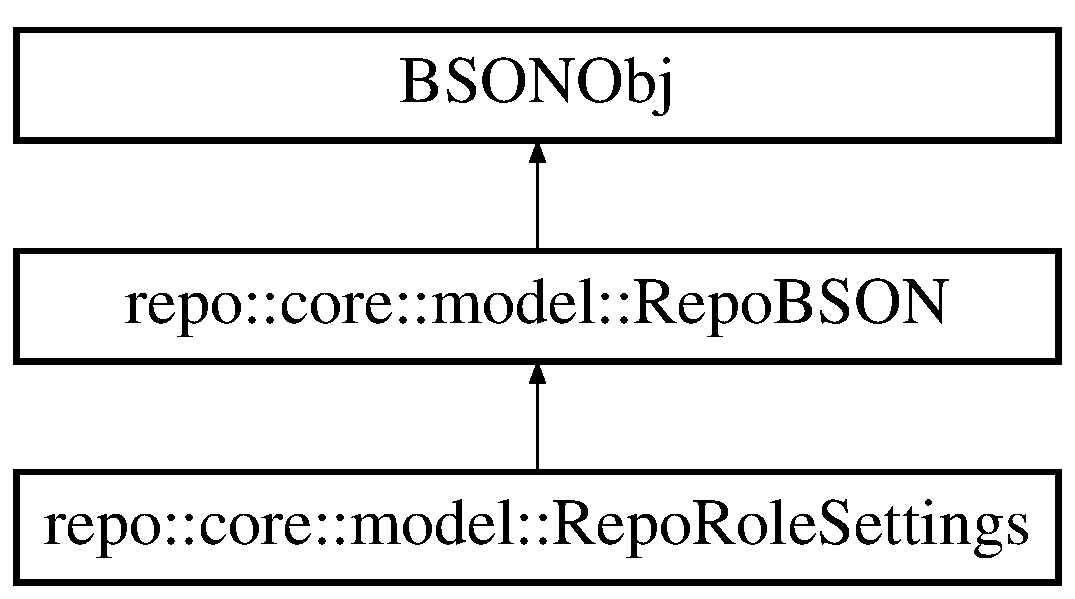
\includegraphics[height=3.000000cm]{classrepo_1_1core_1_1model_1_1_repo_role_settings}
\end{center}
\end{figure}
\subsection*{Public Member Functions}
\begin{DoxyCompactItemize}
\item 
\hypertarget{classrepo_1_1core_1_1model_1_1_repo_role_settings_a544a98aad97a8dfa810c27d426e6d883}{}{\bfseries Repo\+Role\+Settings} (\hyperlink{classrepo_1_1core_1_1model_1_1_repo_b_s_o_n}{Repo\+B\+S\+O\+N} bson)\label{classrepo_1_1core_1_1model_1_1_repo_role_settings_a544a98aad97a8dfa810c27d426e6d883}

\item 
std\+::string \hyperlink{classrepo_1_1core_1_1model_1_1_repo_role_settings_ad9af14be4518a153fbfa69831c8aec46}{get\+Color} () const 
\item 
std\+::string \hyperlink{classrepo_1_1core_1_1model_1_1_repo_role_settings_a2349b21712bee3b32f8674d9d240e573}{get\+Description} () const 
\item 
std\+::vector$<$ std\+::string $>$ \hyperlink{classrepo_1_1core_1_1model_1_1_repo_role_settings_abed36f2c0e4e99ecef414ae1429b2657}{get\+Modules} () const 
\item 
std\+::string \hyperlink{classrepo_1_1core_1_1model_1_1_repo_role_settings_aad45aed668aaed32dc40c10a234f1524}{get\+Name} () const 
\end{DoxyCompactItemize}
\subsection*{Additional Inherited Members}


\subsection{Member Function Documentation}
\hypertarget{classrepo_1_1core_1_1model_1_1_repo_role_settings_ad9af14be4518a153fbfa69831c8aec46}{}\index{repo\+::core\+::model\+::\+Repo\+Role\+Settings@{repo\+::core\+::model\+::\+Repo\+Role\+Settings}!get\+Color@{get\+Color}}
\index{get\+Color@{get\+Color}!repo\+::core\+::model\+::\+Repo\+Role\+Settings@{repo\+::core\+::model\+::\+Repo\+Role\+Settings}}
\subsubsection[{get\+Color}]{\setlength{\rightskip}{0pt plus 5cm}std\+::string repo\+::core\+::model\+::\+Repo\+Role\+Settings\+::get\+Color (
\begin{DoxyParamCaption}
{}
\end{DoxyParamCaption}
) const\hspace{0.3cm}{\ttfamily [inline]}}\label{classrepo_1_1core_1_1model_1_1_repo_role_settings_ad9af14be4518a153fbfa69831c8aec46}
Get the color of the role from this settings \begin{DoxyReturn}{Returns}
returns role color as \#hex string 
\end{DoxyReturn}
\hypertarget{classrepo_1_1core_1_1model_1_1_repo_role_settings_a2349b21712bee3b32f8674d9d240e573}{}\index{repo\+::core\+::model\+::\+Repo\+Role\+Settings@{repo\+::core\+::model\+::\+Repo\+Role\+Settings}!get\+Description@{get\+Description}}
\index{get\+Description@{get\+Description}!repo\+::core\+::model\+::\+Repo\+Role\+Settings@{repo\+::core\+::model\+::\+Repo\+Role\+Settings}}
\subsubsection[{get\+Description}]{\setlength{\rightskip}{0pt plus 5cm}std\+::string repo\+::core\+::model\+::\+Repo\+Role\+Settings\+::get\+Description (
\begin{DoxyParamCaption}
{}
\end{DoxyParamCaption}
) const\hspace{0.3cm}{\ttfamily [inline]}}\label{classrepo_1_1core_1_1model_1_1_repo_role_settings_a2349b21712bee3b32f8674d9d240e573}
Get the description of the role from this settings \begin{DoxyReturn}{Returns}
returns role description as string 
\end{DoxyReturn}
\hypertarget{classrepo_1_1core_1_1model_1_1_repo_role_settings_abed36f2c0e4e99ecef414ae1429b2657}{}\index{repo\+::core\+::model\+::\+Repo\+Role\+Settings@{repo\+::core\+::model\+::\+Repo\+Role\+Settings}!get\+Modules@{get\+Modules}}
\index{get\+Modules@{get\+Modules}!repo\+::core\+::model\+::\+Repo\+Role\+Settings@{repo\+::core\+::model\+::\+Repo\+Role\+Settings}}
\subsubsection[{get\+Modules}]{\setlength{\rightskip}{0pt plus 5cm}std\+::vector$<$std\+::string$>$ repo\+::core\+::model\+::\+Repo\+Role\+Settings\+::get\+Modules (
\begin{DoxyParamCaption}
{}
\end{DoxyParamCaption}
) const\hspace{0.3cm}{\ttfamily [inline]}}\label{classrepo_1_1core_1_1model_1_1_repo_role_settings_abed36f2c0e4e99ecef414ae1429b2657}
Get the vector of available modules from this settings \begin{DoxyReturn}{Returns}
returns modules as vector of strings 
\end{DoxyReturn}
\hypertarget{classrepo_1_1core_1_1model_1_1_repo_role_settings_aad45aed668aaed32dc40c10a234f1524}{}\index{repo\+::core\+::model\+::\+Repo\+Role\+Settings@{repo\+::core\+::model\+::\+Repo\+Role\+Settings}!get\+Name@{get\+Name}}
\index{get\+Name@{get\+Name}!repo\+::core\+::model\+::\+Repo\+Role\+Settings@{repo\+::core\+::model\+::\+Repo\+Role\+Settings}}
\subsubsection[{get\+Name}]{\setlength{\rightskip}{0pt plus 5cm}std\+::string repo\+::core\+::model\+::\+Repo\+Role\+Settings\+::get\+Name (
\begin{DoxyParamCaption}
{}
\end{DoxyParamCaption}
) const\hspace{0.3cm}{\ttfamily [inline]}}\label{classrepo_1_1core_1_1model_1_1_repo_role_settings_aad45aed668aaed32dc40c10a234f1524}
Get the name of the role for this settings \begin{DoxyReturn}{Returns}
returns role name as string 
\end{DoxyReturn}


The documentation for this class was generated from the following files\+:\begin{DoxyCompactItemize}
\item 
C\+:/\+Users/\+Carmen/3\+D Repo/\+Repo/3drepobouncer/bouncer/src/repo/core/model/bson/repo\+\_\+bson\+\_\+role\+\_\+settings.\+h\item 
C\+:/\+Users/\+Carmen/3\+D Repo/\+Repo/3drepobouncer/bouncer/src/repo/core/model/bson/repo\+\_\+bson\+\_\+role\+\_\+settings.\+cpp\end{DoxyCompactItemize}

\hypertarget{classrepo_1_1core_1_1model_1_1_repo_scene}{}\section{repo\+:\+:core\+:\+:model\+:\+:Repo\+Scene Class Reference}
\label{classrepo_1_1core_1_1model_1_1_repo_scene}\index{repo\+::core\+::model\+::\+Repo\+Scene@{repo\+::core\+::model\+::\+Repo\+Scene}}
Inheritance diagram for repo\+:\+:core\+:\+:model\+:\+:Repo\+Scene\+:\begin{figure}[H]
\begin{center}
\leavevmode
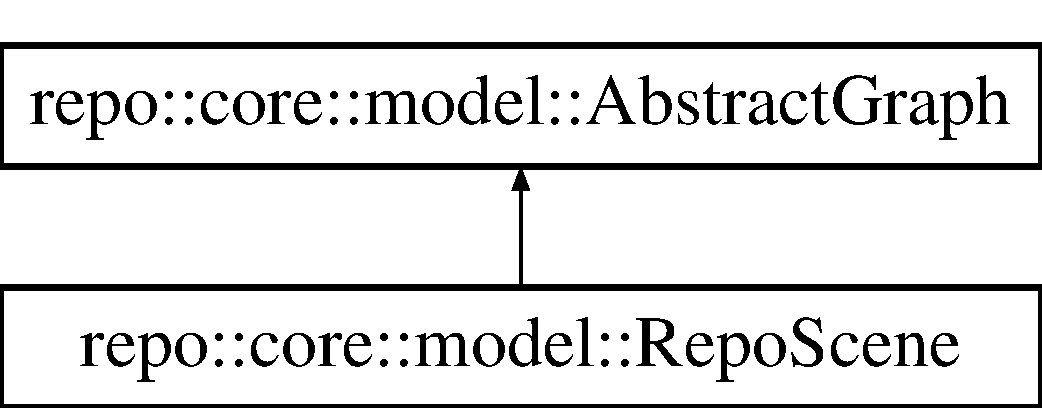
\includegraphics[height=2.000000cm]{classrepo_1_1core_1_1model_1_1_repo_scene}
\end{center}
\end{figure}
\subsection*{Public Types}
\begin{DoxyCompactItemize}
\item 
enum \hyperlink{classrepo_1_1core_1_1model_1_1_repo_scene_aefcacd6eb4c7774ac1bfe3a6b223337c}{Graph\+Type} \{ {\bfseries D\+E\+F\+A\+U\+L\+T}, 
{\bfseries O\+P\+T\+I\+M\+I\+Z\+E\+D}
 \}
\end{DoxyCompactItemize}
\subsection*{Public Member Functions}
\begin{DoxyCompactItemize}
\item 
\hyperlink{classrepo_1_1core_1_1model_1_1_repo_scene_ae56a2c2f4932c2391fb6d9a31031f26c}{Repo\+Scene} (const std\+::string \&database=std\+::string(), const std\+::string \&\hyperlink{classrepo_1_1core_1_1model_1_1_abstract_graph_a8d6f646d8c8d0e5c14b31bbff17a1f1d}{project\+Name}=std\+::string(), const std\+::string \&scene\+Ext=R\+E\+P\+O\+\_\+\+C\+O\+L\+L\+E\+C\+T\+I\+O\+N\+\_\+\+S\+C\+E\+N\+E, const std\+::string \&\hyperlink{classrepo_1_1core_1_1model_1_1_repo_scene_ab33974cb8caec149fdd9743339f4d2ab}{rev\+Ext}=R\+E\+P\+O\+\_\+\+C\+O\+L\+L\+E\+C\+T\+I\+O\+N\+\_\+\+H\+I\+S\+T\+O\+R\+Y, const std\+::string \&\hyperlink{classrepo_1_1core_1_1model_1_1_repo_scene_a9e1ec4f9fa275647a75838361b3d2a5d}{stash\+Ext}=R\+E\+P\+O\+\_\+\+C\+O\+L\+L\+E\+C\+T\+I\+O\+N\+\_\+\+S\+T\+A\+S\+H\+\_\+\+R\+E\+P\+O, const std\+::string \&\hyperlink{classrepo_1_1core_1_1model_1_1_repo_scene_a19be566f3815da34dea4447f4d5b2dba}{raw\+Ext}=R\+E\+P\+O\+\_\+\+C\+O\+L\+L\+E\+C\+T\+I\+O\+N\+\_\+\+R\+A\+W, const std\+::string \&\hyperlink{classrepo_1_1core_1_1model_1_1_repo_scene_ade467377ddb29a8b7ea7347ed81ad0a4}{issues\+Ext}=R\+E\+P\+O\+\_\+\+C\+O\+L\+L\+E\+C\+T\+I\+O\+N\+\_\+\+I\+S\+S\+U\+E\+S, const std\+::string \&\hyperlink{classrepo_1_1core_1_1model_1_1_repo_scene_aaa568af1ee2cde77df38f4c3badb5981}{src\+Ext}=R\+E\+P\+O\+\_\+\+C\+O\+L\+L\+E\+C\+T\+I\+O\+N\+\_\+\+S\+T\+A\+S\+H\+\_\+\+S\+R\+C, const std\+::string \&\hyperlink{classrepo_1_1core_1_1model_1_1_repo_scene_a0de6d5d1c514db0e859b150feb312337}{gltf\+Ext}=R\+E\+P\+O\+\_\+\+C\+O\+L\+L\+E\+C\+T\+I\+O\+N\+\_\+\+S\+T\+A\+S\+H\+\_\+\+G\+L\+T\+F, const std\+::string \&\hyperlink{classrepo_1_1core_1_1model_1_1_repo_scene_ac55e20f143934e73afbca758b8d3d626}{x3d\+Ext}=R\+E\+P\+O\+\_\+\+C\+O\+L\+L\+E\+C\+T\+I\+O\+N\+\_\+\+S\+T\+A\+S\+H\+\_\+\+X3\+D, const std\+::string \&\hyperlink{classrepo_1_1core_1_1model_1_1_repo_scene_a979903ee1680863f4c67cf524bbc6e9f}{json\+Ext}=R\+E\+P\+O\+\_\+\+C\+O\+L\+L\+E\+C\+T\+I\+O\+N\+\_\+\+S\+T\+A\+S\+H\+\_\+\+J\+S\+O\+N)
\item 
\hyperlink{classrepo_1_1core_1_1model_1_1_repo_scene_a2747698490e0fd5db21fdedb2b910b56}{Repo\+Scene} (const std\+::vector$<$ std\+::string $>$ \&\hyperlink{classrepo_1_1core_1_1model_1_1_repo_scene_a72ff48bdd737480c5dd98edb4a39a557}{ref\+Files}, const Repo\+Node\+Set \&cameras, const Repo\+Node\+Set \&meshes, const Repo\+Node\+Set \&materials, const Repo\+Node\+Set \&metadata, const Repo\+Node\+Set \&textures, const Repo\+Node\+Set \&transformations, const Repo\+Node\+Set \&references=Repo\+Node\+Set(), const Repo\+Node\+Set \&maps=Repo\+Node\+Set(), const Repo\+Node\+Set \&unknowns=Repo\+Node\+Set(), const std\+::string \&scene\+Ext=R\+E\+P\+O\+\_\+\+C\+O\+L\+L\+E\+C\+T\+I\+O\+N\+\_\+\+S\+C\+E\+N\+E, const std\+::string \&\hyperlink{classrepo_1_1core_1_1model_1_1_repo_scene_ab33974cb8caec149fdd9743339f4d2ab}{rev\+Ext}=R\+E\+P\+O\+\_\+\+C\+O\+L\+L\+E\+C\+T\+I\+O\+N\+\_\+\+H\+I\+S\+T\+O\+R\+Y, const std\+::string \&\hyperlink{classrepo_1_1core_1_1model_1_1_repo_scene_a9e1ec4f9fa275647a75838361b3d2a5d}{stash\+Ext}=R\+E\+P\+O\+\_\+\+C\+O\+L\+L\+E\+C\+T\+I\+O\+N\+\_\+\+S\+T\+A\+S\+H\+\_\+\+R\+E\+P\+O, const std\+::string \&\hyperlink{classrepo_1_1core_1_1model_1_1_repo_scene_a19be566f3815da34dea4447f4d5b2dba}{raw\+Ext}=R\+E\+P\+O\+\_\+\+C\+O\+L\+L\+E\+C\+T\+I\+O\+N\+\_\+\+R\+A\+W, const std\+::string \&\hyperlink{classrepo_1_1core_1_1model_1_1_repo_scene_ade467377ddb29a8b7ea7347ed81ad0a4}{issues\+Ext}=R\+E\+P\+O\+\_\+\+C\+O\+L\+L\+E\+C\+T\+I\+O\+N\+\_\+\+I\+S\+S\+U\+E\+S, const std\+::string \&\hyperlink{classrepo_1_1core_1_1model_1_1_repo_scene_aaa568af1ee2cde77df38f4c3badb5981}{src\+Ext}=R\+E\+P\+O\+\_\+\+C\+O\+L\+L\+E\+C\+T\+I\+O\+N\+\_\+\+S\+T\+A\+S\+H\+\_\+\+S\+R\+C, const std\+::string \&\hyperlink{classrepo_1_1core_1_1model_1_1_repo_scene_a0de6d5d1c514db0e859b150feb312337}{gltf\+Ext}=R\+E\+P\+O\+\_\+\+C\+O\+L\+L\+E\+C\+T\+I\+O\+N\+\_\+\+S\+T\+A\+S\+H\+\_\+\+G\+L\+T\+F, const std\+::string \&\hyperlink{classrepo_1_1core_1_1model_1_1_repo_scene_ac55e20f143934e73afbca758b8d3d626}{x3d\+Ext}=R\+E\+P\+O\+\_\+\+C\+O\+L\+L\+E\+C\+T\+I\+O\+N\+\_\+\+S\+T\+A\+S\+H\+\_\+\+X3\+D, const std\+::string \&\hyperlink{classrepo_1_1core_1_1model_1_1_repo_scene_a979903ee1680863f4c67cf524bbc6e9f}{json\+Ext}=R\+E\+P\+O\+\_\+\+C\+O\+L\+L\+E\+C\+T\+I\+O\+N\+\_\+\+S\+T\+A\+S\+H\+\_\+\+J\+S\+O\+N)
\item 
\hyperlink{classrepo_1_1core_1_1model_1_1_repo_scene_aadddd2971dbdde53d01d736d77aebedf}{$\sim$\+Repo\+Scene} ()
\item 
bool \hyperlink{classrepo_1_1core_1_1model_1_1_repo_scene_a2ae2f478f17fe7dfeb20ad8befb3b2ee}{is\+O\+K} () const 
\item 
bool \hyperlink{classrepo_1_1core_1_1model_1_1_repo_scene_a826242a71e6bf69893d3287d635442a7}{is\+Missing\+Texture} () const 
\item 
void \hyperlink{classrepo_1_1core_1_1model_1_1_repo_scene_a412be676a80bf9f2594b98bba1924332}{set\+Missing\+Texture} ()
\item 
void \hyperlink{classrepo_1_1core_1_1model_1_1_repo_scene_a0bb2c49fbd8d6c5534b6ef2cf33a45da}{add\+Metadata} (Repo\+Node\+Set \&metadata, const bool \&exact\+Match, const bool \&propagate\+Data=true)
\item 
void \hyperlink{classrepo_1_1core_1_1model_1_1_repo_scene_abd7f9cdc8564aafe868928c467fd0b78}{add\+Stash\+Graph} (const Repo\+Node\+Set \&cameras, const Repo\+Node\+Set \&meshes, const Repo\+Node\+Set \&materials, const Repo\+Node\+Set \&textures, const Repo\+Node\+Set \&transformations)
\item 
void \hyperlink{classrepo_1_1core_1_1model_1_1_repo_scene_ad211f115d0a6d8f398c034ce23384cf1}{clear\+Stash} ()
\item 
bool \hyperlink{classrepo_1_1core_1_1model_1_1_repo_scene_a41aa37ffba3fcd4b2dea7b23a1762644}{commit} (\hyperlink{classrepo_1_1core_1_1handler_1_1_abstract_database_handler}{repo\+::core\+::handler\+::\+Abstract\+Database\+Handler} $\ast$handler, std\+::string \&err\+Msg, const std\+::string \&user\+Name, const std\+::string \&message=std\+::string(), const std\+::string \&tag=std\+::string())
\item 
bool \hyperlink{classrepo_1_1core_1_1model_1_1_repo_scene_a7ec2fae544505ae7d73c458e7c847cd5}{commit\+Stash} (\hyperlink{classrepo_1_1core_1_1handler_1_1_abstract_database_handler}{repo\+::core\+::handler\+::\+Abstract\+Database\+Handler} $\ast$handler, std\+::string \&err\+Msg)
\item 
repo\+U\+U\+I\+D \hyperlink{classrepo_1_1core_1_1model_1_1_repo_scene_aa4ac0636da7d8d27d9615bd6e23ac484}{get\+Branch\+I\+D} () const 
\item 
std\+::string \hyperlink{classrepo_1_1core_1_1model_1_1_repo_scene_a21ac57fcfca6cedcc2aeddce7938c809}{get\+Database\+Name} () const 
\item 
std\+::string \hyperlink{classrepo_1_1core_1_1model_1_1_repo_scene_a6307f0c0df32f10d603028a75afb8e50}{get\+Stash\+Extension} () const 
\item 
std\+::string \hyperlink{classrepo_1_1core_1_1model_1_1_repo_scene_a4606af3c279123479cd7b2bf120c7bbe}{get\+Raw\+Extension} () const 
\item 
std\+::string \hyperlink{classrepo_1_1core_1_1model_1_1_repo_scene_a1a5748642960ad1ae321046eaf7c92eb}{get\+S\+R\+C\+Extension} () const 
\item 
std\+::string \hyperlink{classrepo_1_1core_1_1model_1_1_repo_scene_a656d124c4a6fcb3ea4725928cccc17b6}{get\+G\+L\+T\+F\+Extension} () const 
\item 
std\+::string \hyperlink{classrepo_1_1core_1_1model_1_1_repo_scene_aff5298094e5c75f27b71a9369300f028}{get\+X3\+D\+Extension} () const 
\item 
std\+::string \hyperlink{classrepo_1_1core_1_1model_1_1_repo_scene_aa348500c35ed75184ba4b49c0ecab775}{get\+J\+S\+O\+N\+Extension} () const 
\item 
repo\+U\+U\+I\+D \hyperlink{classrepo_1_1core_1_1model_1_1_repo_scene_aae6865fe4b3c52ab55d04f162ca1b7bf}{get\+Revision\+I\+D} () const 
\item 
std\+::string \hyperlink{classrepo_1_1core_1_1model_1_1_repo_scene_a9d43a9e2ff7e75bc759f475b09d38b70}{get\+Owner} () const 
\item 
std\+::string \hyperlink{classrepo_1_1core_1_1model_1_1_repo_scene_abfdb99dde6895c7226c3514218728bca}{get\+Project\+Name} () const 
\item 
std\+::vector$<$ double $>$ \hyperlink{classrepo_1_1core_1_1model_1_1_repo_scene_ad577dfbbb9da631406933437bc456f37}{get\+World\+Offset} () const 
\item 
bool \hyperlink{classrepo_1_1core_1_1model_1_1_repo_scene_a3c6968fb82e20a6694c1be5170a0bc2b}{is\+Head\+Revision} () const 
\item 
bool \hyperlink{classrepo_1_1core_1_1model_1_1_repo_scene_a8d69fafb52e9a73548d7c22ebbcb562c}{is\+Revisioned} () const 
\item 
void \hyperlink{classrepo_1_1core_1_1model_1_1_repo_scene_a01d7c23a6df5b726b636c518a5a72a35}{set\+Database\+And\+Project\+Name} (std\+::string new\+Database\+Name, std\+::string new\+Project\+Name)
\item 
void \hyperlink{classrepo_1_1core_1_1model_1_1_repo_scene_a0782d1edcdf37539614f93fe7a1fdc0f}{set\+Revision} (repo\+U\+U\+I\+D revision\+I\+D)
\item 
void \hyperlink{classrepo_1_1core_1_1model_1_1_repo_scene_ac2caff05d438979474b4e393edce1ccd}{set\+Branch} (repo\+U\+U\+I\+D branch\+I\+D)
\item 
void \hyperlink{classrepo_1_1core_1_1model_1_1_repo_scene_a346ae9182f19ed55b48c377523dc35ee}{set\+Commit\+Message} (const std\+::string \&msg)
\item 
void \hyperlink{classrepo_1_1core_1_1model_1_1_repo_scene_a617eb9c5266a174cf6f9f0a41dfb115e}{set\+World\+Offset} (const std\+::vector$<$ double $>$ \&offset)
\item 
std\+::string \hyperlink{classrepo_1_1core_1_1model_1_1_repo_scene_a045fd45a5c75176bb193a470f0fcf618}{get\+Branch\+Name} () const 
\item 
\hyperlink{classrepo_1_1core_1_1model_1_1_repo_scene_aefcacd6eb4c7774ac1bfe3a6b223337c}{Graph\+Type} \hyperlink{classrepo_1_1core_1_1model_1_1_repo_scene_a740ff35cf44e9a39a068bdc4a1353cf0}{get\+View\+Graph} () const 
\item 
bool \hyperlink{classrepo_1_1core_1_1model_1_1_repo_scene_a383afae13ad7cd1b64302191b0e4cdd7}{load\+Revision} (\hyperlink{classrepo_1_1core_1_1handler_1_1_abstract_database_handler}{repo\+::core\+::handler\+::\+Abstract\+Database\+Handler} $\ast$handler, std\+::string \&err\+Msg)
\item 
bool \hyperlink{classrepo_1_1core_1_1model_1_1_repo_scene_aae5c18cc8197d8fcd26cc252e4ef9dcc}{load\+Scene} (\hyperlink{classrepo_1_1core_1_1handler_1_1_abstract_database_handler}{repo\+::core\+::handler\+::\+Abstract\+Database\+Handler} $\ast$handler, std\+::string \&err\+Msg)
\item 
bool \hyperlink{classrepo_1_1core_1_1model_1_1_repo_scene_a6affae3bf21f89793b98e883bc084298}{load\+Stash} (\hyperlink{classrepo_1_1core_1_1handler_1_1_abstract_database_handler}{repo\+::core\+::handler\+::\+Abstract\+Database\+Handler} $\ast$handler, std\+::string \&err\+Msg)
\item 
void \hyperlink{classrepo_1_1core_1_1model_1_1_repo_scene_ac85354a3447d62bfc8aad76c5e51d187}{update\+Revision\+Status} (\hyperlink{classrepo_1_1core_1_1handler_1_1_abstract_database_handler}{repo\+::core\+::handler\+::\+Abstract\+Database\+Handler} $\ast$handler, const Revision\+Node\+::\+Upload\+Status \&status)
\item 
void \hyperlink{classrepo_1_1core_1_1model_1_1_repo_scene_addb2548a816916c09d57a9ff5cb54aea}{print\+Statistics} (std\+::iostream \&output)
\item 
void \hyperlink{classrepo_1_1core_1_1model_1_1_repo_scene_aa35a3fdeec65b4ce71b50291cb6732e4}{abandon\+Child} (const \hyperlink{classrepo_1_1core_1_1model_1_1_repo_scene_aefcacd6eb4c7774ac1bfe3a6b223337c}{Graph\+Type} \&g\+Type, const repo\+U\+U\+I\+D \&parent, const repo\+U\+U\+I\+D \&child, const bool \&modify\+Parent=true, const bool \&modify\+Child=true)
\item 
void \hyperlink{classrepo_1_1core_1_1model_1_1_repo_scene_abbcb804184b739134a091c2893b350a5}{abandon\+Child} (const \hyperlink{classrepo_1_1core_1_1model_1_1_repo_scene_aefcacd6eb4c7774ac1bfe3a6b223337c}{Graph\+Type} \&g\+Type, const repo\+U\+U\+I\+D \&parent, \hyperlink{classrepo_1_1core_1_1model_1_1_repo_node}{Repo\+Node} $\ast$child, const bool \&modify\+Parent=true, const bool \&modify\+Child=true)
\item 
void \hyperlink{classrepo_1_1core_1_1model_1_1_repo_scene_a2c207776463353a6eafd430914838a97}{add\+Inheritance} (const \hyperlink{classrepo_1_1core_1_1model_1_1_repo_scene_aefcacd6eb4c7774ac1bfe3a6b223337c}{Graph\+Type} \&g\+Type, const repo\+U\+U\+I\+D \&parent, const repo\+U\+U\+I\+D \&child, const bool \&no\+Update=false)
\item 
void \hyperlink{classrepo_1_1core_1_1model_1_1_repo_scene_a7a4c10fe8521f9c06f492b11ab6a825c}{add\+Inheritance} (const \hyperlink{classrepo_1_1core_1_1model_1_1_repo_scene_aefcacd6eb4c7774ac1bfe3a6b223337c}{Graph\+Type} \&g\+Type, const \hyperlink{classrepo_1_1core_1_1model_1_1_repo_node}{Repo\+Node} $\ast$parent, \hyperlink{classrepo_1_1core_1_1model_1_1_repo_node}{Repo\+Node} $\ast$child, const bool \&no\+Update=false)
\item 
std\+::vector$<$ \hyperlink{classrepo_1_1core_1_1model_1_1_repo_node}{Repo\+Node} $\ast$ $>$ \hyperlink{classrepo_1_1core_1_1model_1_1_repo_scene_a829df4beb0d3edcdfbb9c6445f8a4704}{get\+Children\+As\+Nodes} (const \hyperlink{classrepo_1_1core_1_1model_1_1_repo_scene_aefcacd6eb4c7774ac1bfe3a6b223337c}{Graph\+Type} \&g, const repo\+U\+U\+I\+D \&parent) const 
\item 
std\+::vector$<$ \hyperlink{classrepo_1_1core_1_1model_1_1_repo_node}{Repo\+Node} $\ast$ $>$ \hyperlink{classrepo_1_1core_1_1model_1_1_repo_scene_a0b2a95dc5643d39fd2d65f65ccbecbc4}{get\+Children\+Nodes\+Filtered} (const \hyperlink{classrepo_1_1core_1_1model_1_1_repo_scene_aefcacd6eb4c7774ac1bfe3a6b223337c}{Graph\+Type} \&g, const repo\+U\+U\+I\+D \&parent, const Node\+Type \&type) const 
\item 
std\+::vector$<$ \hyperlink{classrepo_1_1core_1_1model_1_1_repo_node}{Repo\+Node} $\ast$ $>$ \hyperlink{classrepo_1_1core_1_1model_1_1_repo_scene_a722d51e5ef017ca8ea56632f8783b26d}{get\+Parent\+Nodes\+Filtered} (const \hyperlink{classrepo_1_1core_1_1model_1_1_repo_scene_aefcacd6eb4c7774ac1bfe3a6b223337c}{Graph\+Type} \&g\+Type, const \hyperlink{classrepo_1_1core_1_1model_1_1_repo_node}{Repo\+Node} $\ast$node, const Node\+Type \&type) const 
\item 
\hyperlink{classrepo_1_1core_1_1model_1_1_repo_scene}{Repo\+Scene} $\ast$ \hyperlink{classrepo_1_1core_1_1model_1_1_repo_scene_a189b939059994f16c99b67409bdcebf5}{get\+Scene\+From\+Reference} (const \hyperlink{classrepo_1_1core_1_1model_1_1_repo_scene_aefcacd6eb4c7774ac1bfe3a6b223337c}{Graph\+Type} \&g\+Type, const repo\+U\+U\+I\+D \&reference) const 
\item 
std\+::string \hyperlink{classrepo_1_1core_1_1model_1_1_repo_scene_a781f11c7e9f9e561772581fbc8ecd51f}{get\+Texture\+I\+D\+For\+Mesh} (const \hyperlink{classrepo_1_1core_1_1model_1_1_repo_scene_aefcacd6eb4c7774ac1bfe3a6b223337c}{Graph\+Type} \&g\+Type, const repo\+U\+U\+I\+D \&shared\+I\+D) const 
\item 
Repo\+Node\+Set \hyperlink{classrepo_1_1core_1_1model_1_1_repo_scene_a22211b64fc734e3ad198fc3a3ba9cb8c}{get\+All\+Cameras} (const \hyperlink{classrepo_1_1core_1_1model_1_1_repo_scene_aefcacd6eb4c7774ac1bfe3a6b223337c}{Graph\+Type} \&g\+Type) const 
\item 
Repo\+Node\+Set \hyperlink{classrepo_1_1core_1_1model_1_1_repo_scene_adabb0d805be8ec6d7434503ca30d5190}{get\+All\+Materials} (const \hyperlink{classrepo_1_1core_1_1model_1_1_repo_scene_aefcacd6eb4c7774ac1bfe3a6b223337c}{Graph\+Type} \&g\+Type) const 
\item 
Repo\+Node\+Set \hyperlink{classrepo_1_1core_1_1model_1_1_repo_scene_a19e434c83664ce8495b6228d558abbe9}{get\+All\+Maps} (const \hyperlink{classrepo_1_1core_1_1model_1_1_repo_scene_aefcacd6eb4c7774ac1bfe3a6b223337c}{Graph\+Type} \&g\+Type=Graph\+Type\+::\+D\+E\+F\+A\+U\+L\+T) const 
\item 
Repo\+Node\+Set \hyperlink{classrepo_1_1core_1_1model_1_1_repo_scene_add6e2061525f8068419f8179b19ff67b}{get\+All\+Meshes} (const \hyperlink{classrepo_1_1core_1_1model_1_1_repo_scene_aefcacd6eb4c7774ac1bfe3a6b223337c}{Graph\+Type} \&g\+Type) const 
\item 
Repo\+Node\+Set \hyperlink{classrepo_1_1core_1_1model_1_1_repo_scene_a71138b088048664ef380a4b92c800570}{get\+All\+Metadata} (const \hyperlink{classrepo_1_1core_1_1model_1_1_repo_scene_aefcacd6eb4c7774ac1bfe3a6b223337c}{Graph\+Type} \&g\+Type) const 
\item 
Repo\+Node\+Set \hyperlink{classrepo_1_1core_1_1model_1_1_repo_scene_a6dafc1e4f714a1b01cf75609a8c273a2}{get\+All\+References} (const \hyperlink{classrepo_1_1core_1_1model_1_1_repo_scene_aefcacd6eb4c7774ac1bfe3a6b223337c}{Graph\+Type} \&g\+Type) const 
\item 
Repo\+Node\+Set \hyperlink{classrepo_1_1core_1_1model_1_1_repo_scene_a3278ebb3963f43cf1b978cf6cfa7e28a}{get\+All\+Textures} (const \hyperlink{classrepo_1_1core_1_1model_1_1_repo_scene_aefcacd6eb4c7774ac1bfe3a6b223337c}{Graph\+Type} \&g\+Type) const 
\item 
Repo\+Node\+Set \hyperlink{classrepo_1_1core_1_1model_1_1_repo_scene_a2f60a1976f3c0b26f48f88a2e9ea9532}{get\+All\+Transformations} (const \hyperlink{classrepo_1_1core_1_1model_1_1_repo_scene_aefcacd6eb4c7774ac1bfe3a6b223337c}{Graph\+Type} \&g\+Type) const 
\item 
std\+::vector$<$ repo\+U\+U\+I\+D $>$ \hyperlink{classrepo_1_1core_1_1model_1_1_repo_scene_a196bf70ee860e58e79cf4338e61d4aed}{get\+Added\+Nodes\+I\+D} () const 
\item 
\hypertarget{classrepo_1_1core_1_1model_1_1_repo_scene_acddce29a3142eea2ae7d16dd24688013}{}std\+::set$<$ repo\+U\+U\+I\+D $>$ {\bfseries get\+All\+Shared\+I\+Ds} (const \hyperlink{classrepo_1_1core_1_1model_1_1_repo_scene_aefcacd6eb4c7774ac1bfe3a6b223337c}{Graph\+Type} \&g\+Type) const \label{classrepo_1_1core_1_1model_1_1_repo_scene_acddce29a3142eea2ae7d16dd24688013}

\item 
std\+::vector$<$ \hyperlink{classrepo_1_1core_1_1model_1_1_repo_node}{Repo\+Node} $\ast$ $>$ \hyperlink{classrepo_1_1core_1_1model_1_1_repo_scene_a6ca791f3a220139683a483c77b117205}{get\+All\+Descendants\+By\+Type} (const \hyperlink{classrepo_1_1core_1_1model_1_1_repo_scene_aefcacd6eb4c7774ac1bfe3a6b223337c}{Graph\+Type} \&g\+Type, const repo\+U\+U\+I\+D \&shared\+I\+D, const Node\+Type \&type) const 
\item 
std\+::vector$<$ repo\+U\+U\+I\+D $>$ \hyperlink{classrepo_1_1core_1_1model_1_1_repo_scene_a38b387913f5f84bd0b6948b88b5b2a09}{get\+Modified\+Nodes\+I\+D} () const 
\item 
std\+::vector$<$ repo\+U\+U\+I\+D $>$ \hyperlink{classrepo_1_1core_1_1model_1_1_repo_scene_a5eab7b960b71528e609187848c39bec6}{get\+Removed\+Nodes\+I\+D} () const 
\item 
std\+::vector$<$ \hyperlink{classrepo_1_1core_1_1model_1_1_repo_node}{Repo\+Node} $\ast$ $>$ \hyperlink{classrepo_1_1core_1_1model_1_1_repo_scene_a59dd8d61c75867f3b42430c578bbec1f}{get\+Removed\+Nodes} () const 
\item 
std\+::vector$<$ \hyperlink{structrepo__vector__t}{repo\+\_\+vector\+\_\+t} $>$ \hyperlink{classrepo_1_1core_1_1model_1_1_repo_scene_a7de6b4892cf101adf864a4b88cc1984b}{get\+Scene\+Bounding\+Box} () const 
\item 
\hypertarget{classrepo_1_1core_1_1model_1_1_repo_scene_afbca108bafcccbf86660c424afdd1fef}{}size\+\_\+t {\bfseries get\+Total\+Nodes\+Changed} () const \label{classrepo_1_1core_1_1model_1_1_repo_scene_afbca108bafcccbf86660c424afdd1fef}

\item 
\hyperlink{classrepo_1_1core_1_1model_1_1_repo_node}{Repo\+Node} $\ast$ \hyperlink{classrepo_1_1core_1_1model_1_1_repo_scene_ada8d3c259b08a83a2f80b3337b95416d}{get\+Node\+By\+Shared\+I\+D} (const \hyperlink{classrepo_1_1core_1_1model_1_1_repo_scene_aefcacd6eb4c7774ac1bfe3a6b223337c}{Graph\+Type} \&g\+Type, const repo\+U\+U\+I\+D \&shared\+I\+D) const 
\item 
\hyperlink{classrepo_1_1core_1_1model_1_1_repo_node}{Repo\+Node} $\ast$ \hyperlink{classrepo_1_1core_1_1model_1_1_repo_scene_aa15d3e1283014d74816e2aaaec2896f6}{get\+Node\+By\+Unique\+I\+D} (const \hyperlink{classrepo_1_1core_1_1model_1_1_repo_scene_aefcacd6eb4c7774ac1bfe3a6b223337c}{Graph\+Type} \&g\+Type, const repo\+U\+U\+I\+D \&unique\+I\+D) const 
\item 
bool \hyperlink{classrepo_1_1core_1_1model_1_1_repo_scene_a089803365c0d98a9050f36fc0b7b24e4}{has\+Root} (const \hyperlink{classrepo_1_1core_1_1model_1_1_repo_scene_aefcacd6eb4c7774ac1bfe3a6b223337c}{Graph\+Type} \&g\+Type) const 
\item 
\hypertarget{classrepo_1_1core_1_1model_1_1_repo_scene_a29df82d7ec425aeac62bb23c0e5a04a9}{}\hyperlink{classrepo_1_1core_1_1model_1_1_repo_node}{Repo\+Node} $\ast$ {\bfseries get\+Root} (const \hyperlink{classrepo_1_1core_1_1model_1_1_repo_scene_aefcacd6eb4c7774ac1bfe3a6b223337c}{Graph\+Type} \&g\+Type) const \label{classrepo_1_1core_1_1model_1_1_repo_scene_a29df82d7ec425aeac62bb23c0e5a04a9}

\item 
uint32\+\_\+t \hyperlink{classrepo_1_1core_1_1model_1_1_repo_scene_a924528da9d4453284e722b0dc0ca0076}{get\+Items\+In\+Current\+Graph} (const \hyperlink{classrepo_1_1core_1_1model_1_1_repo_scene_aefcacd6eb4c7774ac1bfe3a6b223337c}{Graph\+Type} \&g\+Type)
\item 
std\+::vector$<$ std\+::string $>$ \hyperlink{classrepo_1_1core_1_1model_1_1_repo_scene_a70ca262465b114957590e563b9a0b2d8}{get\+Original\+Files} () const 
\item 
void \hyperlink{classrepo_1_1core_1_1model_1_1_repo_scene_ae0c048bf0904aab3b1f162082724b640}{add\+Nodes} (const std\+::vector$<$ \hyperlink{classrepo_1_1core_1_1model_1_1_repo_node}{Repo\+Node} $\ast$ $>$ \&nodes)
\item 
void \hyperlink{classrepo_1_1core_1_1model_1_1_repo_scene_acf00d158389dc84cc227f2208f053c9b}{modify\+Node} (const \hyperlink{classrepo_1_1core_1_1model_1_1_repo_scene_aefcacd6eb4c7774ac1bfe3a6b223337c}{Graph\+Type} \&gtype, const repo\+U\+U\+I\+D \&shared\+I\+D, \hyperlink{classrepo_1_1core_1_1model_1_1_repo_node}{Repo\+Node} $\ast$new\+Node, const bool \&overwrite=false)
\item 
void \hyperlink{classrepo_1_1core_1_1model_1_1_repo_scene_a932e31fc1448fe8d2bf57c1165cad076}{modify\+Node} (const \hyperlink{classrepo_1_1core_1_1model_1_1_repo_scene_aefcacd6eb4c7774ac1bfe3a6b223337c}{Graph\+Type} \&gtype, \hyperlink{classrepo_1_1core_1_1model_1_1_repo_node}{Repo\+Node} $\ast$node, \hyperlink{classrepo_1_1core_1_1model_1_1_repo_node}{Repo\+Node} $\ast$new\+Node, const bool \&overwrite=false)
\item 
void \hyperlink{classrepo_1_1core_1_1model_1_1_repo_scene_aa51d6a21aaed1aa223ea5413c5c7c853}{remove\+Node} (const \hyperlink{classrepo_1_1core_1_1model_1_1_repo_scene_aefcacd6eb4c7774ac1bfe3a6b223337c}{Graph\+Type} \&gtype, const repo\+U\+U\+I\+D \&shared\+I\+D)
\item 
void \hyperlink{classrepo_1_1core_1_1model_1_1_repo_scene_a49f78b7c17b6e7b4f37a4837edc44e64}{reorientate\+Direct\+X\+Model} ()
\end{DoxyCompactItemize}
\subsection*{Static Public Member Functions}
\begin{DoxyCompactItemize}
\item 
\hypertarget{classrepo_1_1core_1_1model_1_1_repo_scene_a6dd9444bcaf520efbfe085d0193eeab9}{}static std\+::vector$<$ \hyperlink{classrepo_1_1core_1_1model_1_1_repo_node}{Repo\+Node} $\ast$ $>$ {\bfseries filter\+Nodes\+By\+Type} (const std\+::vector$<$ \hyperlink{classrepo_1_1core_1_1model_1_1_repo_node}{Repo\+Node} $\ast$ $>$ nodes, const Node\+Type filter)\label{classrepo_1_1core_1_1model_1_1_repo_scene_a6dd9444bcaf520efbfe085d0193eeab9}

\item 
\hypertarget{classrepo_1_1core_1_1model_1_1_repo_scene_a7207ff3cea12594804131bfc74fa1e01}{}static std\+::vector$<$ std\+::string $>$ {\bfseries get\+Project\+Extensions} ()\label{classrepo_1_1core_1_1model_1_1_repo_scene_a7207ff3cea12594804131bfc74fa1e01}

\end{DoxyCompactItemize}
\subsection*{Protected Member Functions}
\begin{DoxyCompactItemize}
\item 
bool \hyperlink{classrepo_1_1core_1_1model_1_1_repo_scene_aee067257987618315ab9674684c375a1}{add\+Node\+To\+Scene} (const \hyperlink{classrepo_1_1core_1_1model_1_1_repo_scene_aefcacd6eb4c7774ac1bfe3a6b223337c}{Graph\+Type} \&g\+Type, const Repo\+Node\+Set nodes, std\+::string \&err\+Msg, Repo\+Node\+Set $\ast$collection)
\item 
bool \hyperlink{classrepo_1_1core_1_1model_1_1_repo_scene_a1005f9eaa9e3a0bdeb03814b3ed688f9}{add\+Node\+To\+Maps} (const \hyperlink{classrepo_1_1core_1_1model_1_1_repo_scene_aefcacd6eb4c7774ac1bfe3a6b223337c}{Graph\+Type} \&g\+Type, \hyperlink{classrepo_1_1core_1_1model_1_1_repo_node}{Repo\+Node} $\ast$node, std\+::string \&err\+Msg)
\item 
bool \hyperlink{classrepo_1_1core_1_1model_1_1_repo_scene_a37e3a23d88ff4e24bdef2c224c1f6d3f}{commit\+Nodes} (\hyperlink{classrepo_1_1core_1_1handler_1_1_abstract_database_handler}{repo\+::core\+::handler\+::\+Abstract\+Database\+Handler} $\ast$handler, const std\+::vector$<$ repo\+U\+U\+I\+D $>$ \&nodes\+To\+Commit, const \hyperlink{classrepo_1_1core_1_1model_1_1_repo_scene_aefcacd6eb4c7774ac1bfe3a6b223337c}{Graph\+Type} \&g\+Type, std\+::string \&err\+Msg)
\item 
bool \hyperlink{classrepo_1_1core_1_1model_1_1_repo_scene_a3656d3d7e00d3d5513e6a8f356e99bc7}{commit\+Project\+Settings} (\hyperlink{classrepo_1_1core_1_1handler_1_1_abstract_database_handler}{repo\+::core\+::handler\+::\+Abstract\+Database\+Handler} $\ast$handler, std\+::string \&err\+Msg, const std\+::string \&user\+Name)
\item 
bool \hyperlink{classrepo_1_1core_1_1model_1_1_repo_scene_a998e632854f0652dd2a6033055b33c12}{commit\+Revision\+Node} (\hyperlink{classrepo_1_1core_1_1handler_1_1_abstract_database_handler}{repo\+::core\+::handler\+::\+Abstract\+Database\+Handler} $\ast$handler, std\+::string \&err\+Msg, \hyperlink{classrepo_1_1core_1_1model_1_1_revision_node}{Revision\+Node} $\ast$\&new\+Rev\+Node, const std\+::string \&user\+Name, const std\+::string \&message, const std\+::string \&tag)
\item 
bool \hyperlink{classrepo_1_1core_1_1model_1_1_repo_scene_ac00889d23e2887fccad4e57d47bd6356}{commit\+Scene\+Changes} (\hyperlink{classrepo_1_1core_1_1handler_1_1_abstract_database_handler}{repo\+::core\+::handler\+::\+Abstract\+Database\+Handler} $\ast$handler, std\+::string \&err\+Msg)
\item 
void \hyperlink{classrepo_1_1core_1_1model_1_1_repo_scene_af4324820733d5dae30ee3e8e2580af71}{get\+Scene\+Bounding\+Box\+Internal} (const \hyperlink{classrepo_1_1core_1_1model_1_1_repo_scene_aefcacd6eb4c7774ac1bfe3a6b223337c}{Graph\+Type} \&g\+Type, const \hyperlink{classrepo_1_1core_1_1model_1_1_repo_node}{Repo\+Node} $\ast$node, const std\+::vector$<$ float $>$ \&mat, std\+::vector$<$ \hyperlink{structrepo__vector__t}{repo\+\_\+vector\+\_\+t} $>$ \&bbox) const 
\item 
bool \hyperlink{classrepo_1_1core_1_1model_1_1_repo_scene_a35e5705f991f40cdd1e5e16419bcf244}{populate} (const \hyperlink{classrepo_1_1core_1_1model_1_1_repo_scene_aefcacd6eb4c7774ac1bfe3a6b223337c}{Graph\+Type} \&gtype, \hyperlink{classrepo_1_1core_1_1handler_1_1_abstract_database_handler}{repo\+::core\+::handler\+::\+Abstract\+Database\+Handler} $\ast$handler, std\+::vector$<$ \hyperlink{classrepo_1_1core_1_1model_1_1_repo_b_s_o_n}{Repo\+B\+S\+O\+N} $>$ nodes, std\+::string \&err\+Msg)
\item 
void \hyperlink{classrepo_1_1core_1_1model_1_1_repo_scene_a06729da0c472896cac79f0b0ac91d78f}{populate\+And\+Update} (const \hyperlink{classrepo_1_1core_1_1model_1_1_repo_scene_aefcacd6eb4c7774ac1bfe3a6b223337c}{Graph\+Type} \&g\+Type, const Repo\+Node\+Set \&cameras, const Repo\+Node\+Set \&meshes, const Repo\+Node\+Set \&materials, const Repo\+Node\+Set \&metadata, const Repo\+Node\+Set \&textures, const Repo\+Node\+Set \&transformations, const Repo\+Node\+Set \&references, const Repo\+Node\+Set \&maps, const Repo\+Node\+Set \&unknowns)
\item 
void \hyperlink{classrepo_1_1core_1_1model_1_1_repo_scene_adb2dadf1167735dc3116a9265d6b69ee}{shift\+Model} (const std\+::vector$<$ double $>$ \&offset)
\end{DoxyCompactItemize}
\subsection*{Protected Attributes}
\begin{DoxyCompactItemize}
\item 
\hypertarget{classrepo_1_1core_1_1model_1_1_repo_scene_ac8fb04fbc037c6f0836b081d3b47bb26}{}std\+::string {\bfseries scene\+Ext}\label{classrepo_1_1core_1_1model_1_1_repo_scene_ac8fb04fbc037c6f0836b081d3b47bb26}

\item 
std\+::string \hyperlink{classrepo_1_1core_1_1model_1_1_repo_scene_ab33974cb8caec149fdd9743339f4d2ab}{rev\+Ext}
\item 
std\+::string \hyperlink{classrepo_1_1core_1_1model_1_1_repo_scene_a9e1ec4f9fa275647a75838361b3d2a5d}{stash\+Ext}
\item 
std\+::string \hyperlink{classrepo_1_1core_1_1model_1_1_repo_scene_a19be566f3815da34dea4447f4d5b2dba}{raw\+Ext}
\item 
std\+::string \hyperlink{classrepo_1_1core_1_1model_1_1_repo_scene_ade467377ddb29a8b7ea7347ed81ad0a4}{issues\+Ext}
\item 
std\+::string \hyperlink{classrepo_1_1core_1_1model_1_1_repo_scene_aaa568af1ee2cde77df38f4c3badb5981}{src\+Ext}
\item 
std\+::string \hyperlink{classrepo_1_1core_1_1model_1_1_repo_scene_a0de6d5d1c514db0e859b150feb312337}{gltf\+Ext}
\item 
std\+::string \hyperlink{classrepo_1_1core_1_1model_1_1_repo_scene_ac55e20f143934e73afbca758b8d3d626}{x3d\+Ext}
\item 
std\+::string \hyperlink{classrepo_1_1core_1_1model_1_1_repo_scene_a979903ee1680863f4c67cf524bbc6e9f}{json\+Ext}
\item 
std\+::vector$<$ std\+::string $>$ \hyperlink{classrepo_1_1core_1_1model_1_1_repo_scene_a72ff48bdd737480c5dd98edb4a39a557}{ref\+Files}
\item 
\hypertarget{classrepo_1_1core_1_1model_1_1_repo_scene_a7944b62e4b2398cc0dd6041fce738219}{}std\+::vector$<$ \hyperlink{classrepo_1_1core_1_1model_1_1_repo_node}{Repo\+Node} $\ast$ $>$ {\bfseries to\+Remove}\label{classrepo_1_1core_1_1model_1_1_repo_scene_a7944b62e4b2398cc0dd6041fce738219}

\item 
\hypertarget{classrepo_1_1core_1_1model_1_1_repo_scene_ac1d1bedbb3f3e9f54eedcb11f7ec86da}{}std\+::vector$<$ double $>$ {\bfseries world\+Offset}\label{classrepo_1_1core_1_1model_1_1_repo_scene_ac1d1bedbb3f3e9f54eedcb11f7ec86da}

\item 
\hypertarget{classrepo_1_1core_1_1model_1_1_repo_scene_a50b6fa08981d93be82dbb749dd4537ec}{}repo\+U\+U\+I\+D {\bfseries revision}\label{classrepo_1_1core_1_1model_1_1_repo_scene_a50b6fa08981d93be82dbb749dd4537ec}

\item 
\hypertarget{classrepo_1_1core_1_1model_1_1_repo_scene_ae5ebd80162176d41936afe9f798cf34e}{}repo\+U\+U\+I\+D {\bfseries branch}\label{classrepo_1_1core_1_1model_1_1_repo_scene_ae5ebd80162176d41936afe9f798cf34e}

\item 
\hypertarget{classrepo_1_1core_1_1model_1_1_repo_scene_a7984f01694ca36bb810fc76d9e68e34d}{}std\+::string {\bfseries commit\+Msg}\label{classrepo_1_1core_1_1model_1_1_repo_scene_a7984f01694ca36bb810fc76d9e68e34d}

\item 
\hypertarget{classrepo_1_1core_1_1model_1_1_repo_scene_a0eb03888196694950f9890eb3d658d28}{}bool {\bfseries head\+Revision}\label{classrepo_1_1core_1_1model_1_1_repo_scene_a0eb03888196694950f9890eb3d658d28}

\item 
\hypertarget{classrepo_1_1core_1_1model_1_1_repo_scene_a340652907790cb31c3513a4171a52ad1}{}bool {\bfseries un\+Revisioned}\label{classrepo_1_1core_1_1model_1_1_repo_scene_a340652907790cb31c3513a4171a52ad1}

\item 
\hyperlink{classrepo_1_1core_1_1model_1_1_revision_node}{Revision\+Node} $\ast$ \hyperlink{classrepo_1_1core_1_1model_1_1_repo_scene_a8c14ab145d410fb70f0cecec10f8d162}{rev\+Node}
\item 
\hypertarget{classrepo_1_1core_1_1model_1_1_repo_scene_a04915db5b5900d10bcc3bb5f4348276d}{}std\+::set$<$ repo\+U\+U\+I\+D $>$ {\bfseries new\+Current}\label{classrepo_1_1core_1_1model_1_1_repo_scene_a04915db5b5900d10bcc3bb5f4348276d}

\item 
\hypertarget{classrepo_1_1core_1_1model_1_1_repo_scene_a22f146c74245de5112667a178762f7f0}{}std\+::set$<$ repo\+U\+U\+I\+D $>$ {\bfseries new\+Added}\label{classrepo_1_1core_1_1model_1_1_repo_scene_a22f146c74245de5112667a178762f7f0}

\item 
\hypertarget{classrepo_1_1core_1_1model_1_1_repo_scene_a34b581fdb004afc82edb7edd0e2f39d4}{}std\+::set$<$ repo\+U\+U\+I\+D $>$ {\bfseries new\+Removed}\label{classrepo_1_1core_1_1model_1_1_repo_scene_a34b581fdb004afc82edb7edd0e2f39d4}

\item 
\hypertarget{classrepo_1_1core_1_1model_1_1_repo_scene_a80edbb12f455e0ed8d9e9876462bb3e2}{}std\+::set$<$ repo\+U\+U\+I\+D $>$ {\bfseries new\+Modified}\label{classrepo_1_1core_1_1model_1_1_repo_scene_a80edbb12f455e0ed8d9e9876462bb3e2}

\item 
\hypertarget{classrepo_1_1core_1_1model_1_1_repo_scene_a5e10c6cbad07b182d8ee54692b0d003b}{}repo\+Graph\+Instance {\bfseries graph}\label{classrepo_1_1core_1_1model_1_1_repo_scene_a5e10c6cbad07b182d8ee54692b0d003b}

\item 
\hypertarget{classrepo_1_1core_1_1model_1_1_repo_scene_a07a6a53d21f38dce5df162124f07690a}{}repo\+Graph\+Instance {\bfseries stash\+Graph}\label{classrepo_1_1core_1_1model_1_1_repo_scene_a07a6a53d21f38dce5df162124f07690a}

\item 
\hypertarget{classrepo_1_1core_1_1model_1_1_repo_scene_a626174255cd4dcb4072e46d5603ca833}{}uint16\+\_\+t {\bfseries status}\label{classrepo_1_1core_1_1model_1_1_repo_scene_a626174255cd4dcb4072e46d5603ca833}

\end{DoxyCompactItemize}


\subsection{Member Enumeration Documentation}
\hypertarget{classrepo_1_1core_1_1model_1_1_repo_scene_aefcacd6eb4c7774ac1bfe3a6b223337c}{}\index{repo\+::core\+::model\+::\+Repo\+Scene@{repo\+::core\+::model\+::\+Repo\+Scene}!Graph\+Type@{Graph\+Type}}
\index{Graph\+Type@{Graph\+Type}!repo\+::core\+::model\+::\+Repo\+Scene@{repo\+::core\+::model\+::\+Repo\+Scene}}
\subsubsection[{Graph\+Type}]{\setlength{\rightskip}{0pt plus 5cm}enum {\bf repo\+::core\+::model\+::\+Repo\+Scene\+::\+Graph\+Type}\hspace{0.3cm}{\ttfamily [strong]}}\label{classrepo_1_1core_1_1model_1_1_repo_scene_aefcacd6eb4c7774ac1bfe3a6b223337c}
D\+E\+F\+A\+U\+L\+T -\/ The graph that is revisioned -\/ should be (close to) identical to original model O\+P\+T\+I\+M\+I\+Z\+E\+D -\/ The optimized version of the graph -\/ for quick visualization purposes 

\subsection{Constructor \& Destructor Documentation}
\hypertarget{classrepo_1_1core_1_1model_1_1_repo_scene_ae56a2c2f4932c2391fb6d9a31031f26c}{}\index{repo\+::core\+::model\+::\+Repo\+Scene@{repo\+::core\+::model\+::\+Repo\+Scene}!Repo\+Scene@{Repo\+Scene}}
\index{Repo\+Scene@{Repo\+Scene}!repo\+::core\+::model\+::\+Repo\+Scene@{repo\+::core\+::model\+::\+Repo\+Scene}}
\subsubsection[{Repo\+Scene}]{\setlength{\rightskip}{0pt plus 5cm}Repo\+Scene\+::\+Repo\+Scene (
\begin{DoxyParamCaption}
\item[{const std\+::string \&}]{database = {\ttfamily std\+:\+:string()}, }
\item[{const std\+::string \&}]{project\+Name = {\ttfamily std\+:\+:string()}, }
\item[{const std\+::string \&}]{scene\+Ext = {\ttfamily REPO\+\_\+COLLECTION\+\_\+SCENE}, }
\item[{const std\+::string \&}]{rev\+Ext = {\ttfamily REPO\+\_\+COLLECTION\+\_\+HISTORY}, }
\item[{const std\+::string \&}]{stash\+Ext = {\ttfamily REPO\+\_\+COLLECTION\+\_\+STASH\+\_\+REPO}, }
\item[{const std\+::string \&}]{raw\+Ext = {\ttfamily REPO\+\_\+COLLECTION\+\_\+RAW}, }
\item[{const std\+::string \&}]{issues\+Ext = {\ttfamily REPO\+\_\+COLLECTION\+\_\+ISSUES}, }
\item[{const std\+::string \&}]{src\+Ext = {\ttfamily REPO\+\_\+COLLECTION\+\_\+STASH\+\_\+SRC}, }
\item[{const std\+::string \&}]{gltf\+Ext = {\ttfamily REPO\+\_\+COLLECTION\+\_\+STASH\+\_\+GLTF}, }
\item[{const std\+::string \&}]{x3d\+Ext = {\ttfamily REPO\+\_\+COLLECTION\+\_\+STASH\+\_\+X3D}, }
\item[{const std\+::string \&}]{json\+Ext = {\ttfamily REPO\+\_\+COLLECTION\+\_\+STASH\+\_\+JSON}}
\end{DoxyParamCaption}
)}\label{classrepo_1_1core_1_1model_1_1_repo_scene_ae56a2c2f4932c2391fb6d9a31031f26c}
Used for loading scene graphs from database Constructor -\/ instantiates a new scene graph representation. Branch is set to master and Revision is set to head Use \hyperlink{classrepo_1_1core_1_1model_1_1_repo_scene_a0782d1edcdf37539614f93fe7a1fdc0f}{set\+Revision()} and \hyperlink{classrepo_1_1core_1_1model_1_1_repo_scene_ac2caff05d438979474b4e393edce1ccd}{set\+Branch()} to specify which revision to load N\+O\+T\+E\+: This merely sets up the settings of the scene graph the graph itself is not loaded until \hyperlink{classrepo_1_1core_1_1model_1_1_repo_scene_aae5c18cc8197d8fcd26cc252e4ef9dcc}{load\+Scene()} is called!


\begin{DoxyParams}{Parameters}
{\em database} & name of the database \\
\hline
{\em project\+Name} & name of the project \\
\hline
{\em scene\+Ext} & extension name of the scene graph (Default\+: \char`\"{}scene\char`\"{}) \\
\hline
{\em rev\+Ext} & extension name of the revision graph (Default\+: \char`\"{}history\char`\"{}) \\
\hline
{\em stash\+Ext} & extension name of the stash (Default\+: \char`\"{}stash.\+3drepo\char`\"{}) \\
\hline
\end{DoxyParams}
\hypertarget{classrepo_1_1core_1_1model_1_1_repo_scene_a2747698490e0fd5db21fdedb2b910b56}{}\index{repo\+::core\+::model\+::\+Repo\+Scene@{repo\+::core\+::model\+::\+Repo\+Scene}!Repo\+Scene@{Repo\+Scene}}
\index{Repo\+Scene@{Repo\+Scene}!repo\+::core\+::model\+::\+Repo\+Scene@{repo\+::core\+::model\+::\+Repo\+Scene}}
\subsubsection[{Repo\+Scene}]{\setlength{\rightskip}{0pt plus 5cm}Repo\+Scene\+::\+Repo\+Scene (
\begin{DoxyParamCaption}
\item[{const std\+::vector$<$ std\+::string $>$ \&}]{ref\+Files, }
\item[{const Repo\+Node\+Set \&}]{cameras, }
\item[{const Repo\+Node\+Set \&}]{meshes, }
\item[{const Repo\+Node\+Set \&}]{materials, }
\item[{const Repo\+Node\+Set \&}]{metadata, }
\item[{const Repo\+Node\+Set \&}]{textures, }
\item[{const Repo\+Node\+Set \&}]{transformations, }
\item[{const Repo\+Node\+Set \&}]{references = {\ttfamily RepoNodeSet()}, }
\item[{const Repo\+Node\+Set \&}]{maps = {\ttfamily RepoNodeSet()}, }
\item[{const Repo\+Node\+Set \&}]{unknowns = {\ttfamily RepoNodeSet()}, }
\item[{const std\+::string \&}]{scene\+Ext = {\ttfamily REPO\+\_\+COLLECTION\+\_\+SCENE}, }
\item[{const std\+::string \&}]{rev\+Ext = {\ttfamily REPO\+\_\+COLLECTION\+\_\+HISTORY}, }
\item[{const std\+::string \&}]{stash\+Ext = {\ttfamily REPO\+\_\+COLLECTION\+\_\+STASH\+\_\+REPO}, }
\item[{const std\+::string \&}]{raw\+Ext = {\ttfamily REPO\+\_\+COLLECTION\+\_\+RAW}, }
\item[{const std\+::string \&}]{issues\+Ext = {\ttfamily REPO\+\_\+COLLECTION\+\_\+ISSUES}, }
\item[{const std\+::string \&}]{src\+Ext = {\ttfamily REPO\+\_\+COLLECTION\+\_\+STASH\+\_\+SRC}, }
\item[{const std\+::string \&}]{gltf\+Ext = {\ttfamily REPO\+\_\+COLLECTION\+\_\+STASH\+\_\+GLTF}, }
\item[{const std\+::string \&}]{x3d\+Ext = {\ttfamily REPO\+\_\+COLLECTION\+\_\+STASH\+\_\+X3D}, }
\item[{const std\+::string \&}]{json\+Ext = {\ttfamily REPO\+\_\+COLLECTION\+\_\+STASH\+\_\+JSON}}
\end{DoxyParamCaption}
)}\label{classrepo_1_1core_1_1model_1_1_repo_scene_a2747698490e0fd5db21fdedb2b910b56}
Used for constructing scene graphs from model convertors Constructor -\/ instantiates a new scene graph representation. This scene will be flagged as not revisioned. A database handler will need to be set before it can be commited into the database N\+O\+T\+E\+: database handler, project name, database name will need to be set before this scene graph can be commited to the database. 
\begin{DoxyParams}{Parameters}
{\em ref\+Files} & vector of files created this scene \\
\hline
{\em cameras} & Repo Node set of cameras \\
\hline
{\em meshes} & Repo Node set of meshes \\
\hline
{\em materials} & Repo Node set of materials \\
\hline
{\em metadata} & Repo Node set of metadata \\
\hline
{\em textures} & Repo Node set of textures \\
\hline
{\em transformations} & Repo Node set of transformations \\
\hline
{\em references} & Repo Node set of references (optional) \\
\hline
{\em maps} & Repo Node set of maps (optional) \\
\hline
{\em unknowns} & Repo Node set of unknowns (optional) \\
\hline
{\em scene\+Ext} & extension name of the scene when it is saved into the database (optional) \\
\hline
{\em rev\+Ext} & extension name of the revision when it is saved into the database (optional) \\
\hline
{\em stash\+Ext} & extension name of the stash (Default\+: \char`\"{}stash.\+3drepo\char`\"{}) \\
\hline
\end{DoxyParams}
\hypertarget{classrepo_1_1core_1_1model_1_1_repo_scene_aadddd2971dbdde53d01d736d77aebedf}{}\index{repo\+::core\+::model\+::\+Repo\+Scene@{repo\+::core\+::model\+::\+Repo\+Scene}!````~Repo\+Scene@{$\sim$\+Repo\+Scene}}
\index{````~Repo\+Scene@{$\sim$\+Repo\+Scene}!repo\+::core\+::model\+::\+Repo\+Scene@{repo\+::core\+::model\+::\+Repo\+Scene}}
\subsubsection[{$\sim$\+Repo\+Scene}]{\setlength{\rightskip}{0pt plus 5cm}Repo\+Scene\+::$\sim$\+Repo\+Scene (
\begin{DoxyParamCaption}
{}
\end{DoxyParamCaption}
)}\label{classrepo_1_1core_1_1model_1_1_repo_scene_aadddd2971dbdde53d01d736d77aebedf}
Default Deconstructor Please note that destroying the scene graph will also destroy all nodes created by the scene graph and also its child graphs 

\subsection{Member Function Documentation}
\hypertarget{classrepo_1_1core_1_1model_1_1_repo_scene_aa35a3fdeec65b4ce71b50291cb6732e4}{}\index{repo\+::core\+::model\+::\+Repo\+Scene@{repo\+::core\+::model\+::\+Repo\+Scene}!abandon\+Child@{abandon\+Child}}
\index{abandon\+Child@{abandon\+Child}!repo\+::core\+::model\+::\+Repo\+Scene@{repo\+::core\+::model\+::\+Repo\+Scene}}
\subsubsection[{abandon\+Child}]{\setlength{\rightskip}{0pt plus 5cm}void repo\+::core\+::model\+::\+Repo\+Scene\+::abandon\+Child (
\begin{DoxyParamCaption}
\item[{const {\bf Graph\+Type} \&}]{g\+Type, }
\item[{const repo\+U\+U\+I\+D \&}]{parent, }
\item[{const repo\+U\+U\+I\+D \&}]{child, }
\item[{const bool \&}]{modify\+Parent = {\ttfamily true}, }
\item[{const bool \&}]{modify\+Child = {\ttfamily true}}
\end{DoxyParamCaption}
)\hspace{0.3cm}{\ttfamily [inline]}}\label{classrepo_1_1core_1_1model_1_1_repo_scene_aa35a3fdeec65b4ce71b50291cb6732e4}
-\/-\/-\/-\/-\/-\/-\/-\/-\/-\/-\/-\/-\/-\/-\/------ Node Relationship -\/-\/-\/-\/-\/-\/-\/-\/-\/-\/-\/-\/-\/-\/-\/-\/------ Abandon child from parent (disjoint 2 nodes within the scene) 
\begin{DoxyParams}{Parameters}
{\em parent} & shared I\+D of parent \\
\hline
{\em child} & shared I\+D of child \\
\hline
{\em modify\+Parent} & modify parent to relay the information (not needed if this node is to be removed) \\
\hline
{\em modify\+Child} & modify child node to relay this information (not needed if this node is to be removed) \\
\hline
\end{DoxyParams}
\hypertarget{classrepo_1_1core_1_1model_1_1_repo_scene_abbcb804184b739134a091c2893b350a5}{}\index{repo\+::core\+::model\+::\+Repo\+Scene@{repo\+::core\+::model\+::\+Repo\+Scene}!abandon\+Child@{abandon\+Child}}
\index{abandon\+Child@{abandon\+Child}!repo\+::core\+::model\+::\+Repo\+Scene@{repo\+::core\+::model\+::\+Repo\+Scene}}
\subsubsection[{abandon\+Child}]{\setlength{\rightskip}{0pt plus 5cm}void Repo\+Scene\+::abandon\+Child (
\begin{DoxyParamCaption}
\item[{const {\bf Graph\+Type} \&}]{g\+Type, }
\item[{const repo\+U\+U\+I\+D \&}]{parent, }
\item[{{\bf Repo\+Node} $\ast$}]{child, }
\item[{const bool \&}]{modify\+Parent = {\ttfamily true}, }
\item[{const bool \&}]{modify\+Child = {\ttfamily true}}
\end{DoxyParamCaption}
)}\label{classrepo_1_1core_1_1model_1_1_repo_scene_abbcb804184b739134a091c2893b350a5}
Abandon child from parent (disjoint 2 nodes within the scene) 
\begin{DoxyParams}{Parameters}
{\em parent} & shared I\+D of parent \\
\hline
{\em child} & node of child \\
\hline
{\em modify\+Node} & modify child node to relay this information (not needed if this node is to be removed) \\
\hline
\end{DoxyParams}
\hypertarget{classrepo_1_1core_1_1model_1_1_repo_scene_a2c207776463353a6eafd430914838a97}{}\index{repo\+::core\+::model\+::\+Repo\+Scene@{repo\+::core\+::model\+::\+Repo\+Scene}!add\+Inheritance@{add\+Inheritance}}
\index{add\+Inheritance@{add\+Inheritance}!repo\+::core\+::model\+::\+Repo\+Scene@{repo\+::core\+::model\+::\+Repo\+Scene}}
\subsubsection[{add\+Inheritance}]{\setlength{\rightskip}{0pt plus 5cm}void repo\+::core\+::model\+::\+Repo\+Scene\+::add\+Inheritance (
\begin{DoxyParamCaption}
\item[{const {\bf Graph\+Type} \&}]{g\+Type, }
\item[{const repo\+U\+U\+I\+D \&}]{parent, }
\item[{const repo\+U\+U\+I\+D \&}]{child, }
\item[{const bool \&}]{no\+Update = {\ttfamily false}}
\end{DoxyParamCaption}
)\hspace{0.3cm}{\ttfamily [inline]}}\label{classrepo_1_1core_1_1model_1_1_repo_scene_a2c207776463353a6eafd430914838a97}
Introduce parentship to 2 nodes that already reside within the scene. If either of the nodes are not found, it does nothing If they already share an inheritance, it does nothing 
\begin{DoxyParams}{Parameters}
{\em g\+Type} & which graph are the nodes \\
\hline
{\em parent} & U\+N\+I\+Q\+U\+E uuid of the parent \\
\hline
{\em child} & U\+N\+I\+Q\+U\+E uuid of the child \\
\hline
{\em no\+Update} & if true, it will not be treated as a change that is needed to be commited (only valid for default graph) \\
\hline
\end{DoxyParams}
\hypertarget{classrepo_1_1core_1_1model_1_1_repo_scene_a7a4c10fe8521f9c06f492b11ab6a825c}{}\index{repo\+::core\+::model\+::\+Repo\+Scene@{repo\+::core\+::model\+::\+Repo\+Scene}!add\+Inheritance@{add\+Inheritance}}
\index{add\+Inheritance@{add\+Inheritance}!repo\+::core\+::model\+::\+Repo\+Scene@{repo\+::core\+::model\+::\+Repo\+Scene}}
\subsubsection[{add\+Inheritance}]{\setlength{\rightskip}{0pt plus 5cm}void Repo\+Scene\+::add\+Inheritance (
\begin{DoxyParamCaption}
\item[{const {\bf Graph\+Type} \&}]{g\+Type, }
\item[{const {\bf Repo\+Node} $\ast$}]{parent, }
\item[{{\bf Repo\+Node} $\ast$}]{child, }
\item[{const bool \&}]{no\+Update = {\ttfamily false}}
\end{DoxyParamCaption}
)}\label{classrepo_1_1core_1_1model_1_1_repo_scene_a7a4c10fe8521f9c06f492b11ab6a825c}
Introduce parentship to 2 nodes that already reside within the scene. If either of the nodes are not found, it does nothing If they already share an inheritance, it does nothing 
\begin{DoxyParams}{Parameters}
{\em g\+Type} & which graph are the nodes \\
\hline
{\em parent} & parent Node \\
\hline
{\em child} & child node \\
\hline
{\em no\+Update} & if true, it will not be treated as a change that is needed to be commited (only valid for default graph) \\
\hline
\end{DoxyParams}
\hypertarget{classrepo_1_1core_1_1model_1_1_repo_scene_a0bb2c49fbd8d6c5534b6ef2cf33a45da}{}\index{repo\+::core\+::model\+::\+Repo\+Scene@{repo\+::core\+::model\+::\+Repo\+Scene}!add\+Metadata@{add\+Metadata}}
\index{add\+Metadata@{add\+Metadata}!repo\+::core\+::model\+::\+Repo\+Scene@{repo\+::core\+::model\+::\+Repo\+Scene}}
\subsubsection[{add\+Metadata}]{\setlength{\rightskip}{0pt plus 5cm}void Repo\+Scene\+::add\+Metadata (
\begin{DoxyParamCaption}
\item[{Repo\+Node\+Set \&}]{metadata, }
\item[{const bool \&}]{exact\+Match, }
\item[{const bool \&}]{propagate\+Data = {\ttfamily true}}
\end{DoxyParamCaption}
)}\label{classrepo_1_1core_1_1model_1_1_repo_scene_a0bb2c49fbd8d6c5534b6ef2cf33a45da}
Add metadata that has a matching name as the transformation into the scene 
\begin{DoxyParams}{Parameters}
{\em metadata} & set of metadata to attach \\
\hline
{\em exact\+Match} & whether the name has to be an exact match or a substring will do \\
\hline
{\em propagate\+Data} & if set to true, propagate down the changes to all meshes of this subtree \\
\hline
\end{DoxyParams}
\hypertarget{classrepo_1_1core_1_1model_1_1_repo_scene_ae0c048bf0904aab3b1f162082724b640}{}\index{repo\+::core\+::model\+::\+Repo\+Scene@{repo\+::core\+::model\+::\+Repo\+Scene}!add\+Nodes@{add\+Nodes}}
\index{add\+Nodes@{add\+Nodes}!repo\+::core\+::model\+::\+Repo\+Scene@{repo\+::core\+::model\+::\+Repo\+Scene}}
\subsubsection[{add\+Nodes}]{\setlength{\rightskip}{0pt plus 5cm}void Repo\+Scene\+::add\+Nodes (
\begin{DoxyParamCaption}
\item[{const std\+::vector$<$ {\bf Repo\+Node} $\ast$ $>$ \&}]{nodes}
\end{DoxyParamCaption}
)}\label{classrepo_1_1core_1_1model_1_1_repo_scene_ae0c048bf0904aab3b1f162082724b640}
-\/-\/-\/-\/-\/-\/-\/-\/------ Scene Modification Functions -\/-\/-\/-\/-\/-\/-\/-\/------ Add a vector of nodes into the unoptimized scene graph Tracks the modification for commit 
\begin{DoxyParams}{Parameters}
{\em vector} & of nodes to insert. \\
\hline
\end{DoxyParams}
\hypertarget{classrepo_1_1core_1_1model_1_1_repo_scene_a1005f9eaa9e3a0bdeb03814b3ed688f9}{}\index{repo\+::core\+::model\+::\+Repo\+Scene@{repo\+::core\+::model\+::\+Repo\+Scene}!add\+Node\+To\+Maps@{add\+Node\+To\+Maps}}
\index{add\+Node\+To\+Maps@{add\+Node\+To\+Maps}!repo\+::core\+::model\+::\+Repo\+Scene@{repo\+::core\+::model\+::\+Repo\+Scene}}
\subsubsection[{add\+Node\+To\+Maps}]{\setlength{\rightskip}{0pt plus 5cm}bool Repo\+Scene\+::add\+Node\+To\+Maps (
\begin{DoxyParamCaption}
\item[{const {\bf Graph\+Type} \&}]{g\+Type, }
\item[{{\bf Repo\+Node} $\ast$}]{node, }
\item[{std\+::string \&}]{err\+Msg}
\end{DoxyParamCaption}
)\hspace{0.3cm}{\ttfamily [protected]}}\label{classrepo_1_1core_1_1model_1_1_repo_scene_a1005f9eaa9e3a0bdeb03814b3ed688f9}
Add node to the following maps\+: Unique\+I\+D -\/$>$ Node, Shared\+I\+D -\/$>$ Unique\+I\+D, Parent-\/$>$Children. It will also assign root node if the node has no parent. 
\begin{DoxyParams}{Parameters}
{\em g} & which graph to insert into \\
\hline
{\em node} & pointer to the node to add \\
\hline
{\em err\+Msg} & error message if it returns false \\
\hline
\end{DoxyParams}
\begin{DoxyReturn}{Returns}
returns true if succeeded 
\end{DoxyReturn}
\hypertarget{classrepo_1_1core_1_1model_1_1_repo_scene_aee067257987618315ab9674684c375a1}{}\index{repo\+::core\+::model\+::\+Repo\+Scene@{repo\+::core\+::model\+::\+Repo\+Scene}!add\+Node\+To\+Scene@{add\+Node\+To\+Scene}}
\index{add\+Node\+To\+Scene@{add\+Node\+To\+Scene}!repo\+::core\+::model\+::\+Repo\+Scene@{repo\+::core\+::model\+::\+Repo\+Scene}}
\subsubsection[{add\+Node\+To\+Scene}]{\setlength{\rightskip}{0pt plus 5cm}bool Repo\+Scene\+::add\+Node\+To\+Scene (
\begin{DoxyParamCaption}
\item[{const {\bf Graph\+Type} \&}]{g\+Type, }
\item[{const Repo\+Node\+Set}]{nodes, }
\item[{std\+::string \&}]{err\+Msg, }
\item[{Repo\+Node\+Set $\ast$}]{collection}
\end{DoxyParamCaption}
)\hspace{0.3cm}{\ttfamily [protected]}}\label{classrepo_1_1core_1_1model_1_1_repo_scene_aee067257987618315ab9674684c375a1}




Add Nodes to scene. 
\begin{DoxyParams}{Parameters}
{\em g\+Type} & which graph to add the nodes onto (default or optimized) \\
\hline
{\em node} & pointer to the node to add \\
\hline
{\em err\+Msg} & error message if it returns false \\
\hline
{\em collection} & the collection for the node type if known. \\
\hline
\end{DoxyParams}
\begin{DoxyReturn}{Returns}
returns true if succeeded 
\end{DoxyReturn}
\hypertarget{classrepo_1_1core_1_1model_1_1_repo_scene_abd7f9cdc8564aafe868928c467fd0b78}{}\index{repo\+::core\+::model\+::\+Repo\+Scene@{repo\+::core\+::model\+::\+Repo\+Scene}!add\+Stash\+Graph@{add\+Stash\+Graph}}
\index{add\+Stash\+Graph@{add\+Stash\+Graph}!repo\+::core\+::model\+::\+Repo\+Scene@{repo\+::core\+::model\+::\+Repo\+Scene}}
\subsubsection[{add\+Stash\+Graph}]{\setlength{\rightskip}{0pt plus 5cm}void Repo\+Scene\+::add\+Stash\+Graph (
\begin{DoxyParamCaption}
\item[{const Repo\+Node\+Set \&}]{cameras, }
\item[{const Repo\+Node\+Set \&}]{meshes, }
\item[{const Repo\+Node\+Set \&}]{materials, }
\item[{const Repo\+Node\+Set \&}]{textures, }
\item[{const Repo\+Node\+Set \&}]{transformations}
\end{DoxyParamCaption}
)}\label{classrepo_1_1core_1_1model_1_1_repo_scene_abd7f9cdc8564aafe868928c467fd0b78}
Add a stash graph (optimised graph) for the corresponding scene graph 
\begin{DoxyParams}{Parameters}
{\em camera} & set of cameras \\
\hline
{\em meshes} & set of meshes \\
\hline
{\em materials} & set of materials \\
\hline
{\em textures} & set of textures \\
\hline
{\em transformations} & set of transformations \\
\hline
\end{DoxyParams}
\hypertarget{classrepo_1_1core_1_1model_1_1_repo_scene_ad211f115d0a6d8f398c034ce23384cf1}{}\index{repo\+::core\+::model\+::\+Repo\+Scene@{repo\+::core\+::model\+::\+Repo\+Scene}!clear\+Stash@{clear\+Stash}}
\index{clear\+Stash@{clear\+Stash}!repo\+::core\+::model\+::\+Repo\+Scene@{repo\+::core\+::model\+::\+Repo\+Scene}}
\subsubsection[{clear\+Stash}]{\setlength{\rightskip}{0pt plus 5cm}void Repo\+Scene\+::clear\+Stash (
\begin{DoxyParamCaption}
{}
\end{DoxyParamCaption}
)}\label{classrepo_1_1core_1_1model_1_1_repo_scene_ad211f115d0a6d8f398c034ce23384cf1}
Clears the contents within the Stash (if there is one) \hypertarget{classrepo_1_1core_1_1model_1_1_repo_scene_a41aa37ffba3fcd4b2dea7b23a1762644}{}\index{repo\+::core\+::model\+::\+Repo\+Scene@{repo\+::core\+::model\+::\+Repo\+Scene}!commit@{commit}}
\index{commit@{commit}!repo\+::core\+::model\+::\+Repo\+Scene@{repo\+::core\+::model\+::\+Repo\+Scene}}
\subsubsection[{commit}]{\setlength{\rightskip}{0pt plus 5cm}bool Repo\+Scene\+::commit (
\begin{DoxyParamCaption}
\item[{{\bf repo\+::core\+::handler\+::\+Abstract\+Database\+Handler} $\ast$}]{handler, }
\item[{std\+::string \&}]{err\+Msg, }
\item[{const std\+::string \&}]{user\+Name, }
\item[{const std\+::string \&}]{message = {\ttfamily std\+:\+:string()}, }
\item[{const std\+::string \&}]{tag = {\ttfamily std\+:\+:string()}}
\end{DoxyParamCaption}
)}\label{classrepo_1_1core_1_1model_1_1_repo_scene_a41aa37ffba3fcd4b2dea7b23a1762644}
Commit changes on the default graph into the database This commits an update to project settings, a new revision node and the changes within this scene 
\begin{DoxyParams}{Parameters}
{\em err\+Msg} & error message if this failed \\
\hline
{\em user\+Name} & name of the author \\
\hline
{\em message} & message for this commit (optional) \\
\hline
{\em tag} & tag for this commit (optional) \\
\hline
\end{DoxyParams}
\begin{DoxyReturn}{Returns}
returns true upon success 
\end{DoxyReturn}
\hypertarget{classrepo_1_1core_1_1model_1_1_repo_scene_a37e3a23d88ff4e24bdef2c224c1f6d3f}{}\index{repo\+::core\+::model\+::\+Repo\+Scene@{repo\+::core\+::model\+::\+Repo\+Scene}!commit\+Nodes@{commit\+Nodes}}
\index{commit\+Nodes@{commit\+Nodes}!repo\+::core\+::model\+::\+Repo\+Scene@{repo\+::core\+::model\+::\+Repo\+Scene}}
\subsubsection[{commit\+Nodes}]{\setlength{\rightskip}{0pt plus 5cm}bool Repo\+Scene\+::commit\+Nodes (
\begin{DoxyParamCaption}
\item[{{\bf repo\+::core\+::handler\+::\+Abstract\+Database\+Handler} $\ast$}]{handler, }
\item[{const std\+::vector$<$ repo\+U\+U\+I\+D $>$ \&}]{nodes\+To\+Commit, }
\item[{const {\bf Graph\+Type} \&}]{g\+Type, }
\item[{std\+::string \&}]{err\+Msg}
\end{DoxyParamCaption}
)\hspace{0.3cm}{\ttfamily [protected]}}\label{classrepo_1_1core_1_1model_1_1_repo_scene_a37e3a23d88ff4e24bdef2c224c1f6d3f}
Commit a vector of nodes into the database 
\begin{DoxyParams}{Parameters}
{\em handler} & database handler to perform the commit \\
\hline
{\em nodes\+To\+Commit} & vector of uuids of nodes to commit \\
\hline
{\em graph\+Type} & which graph did the nodes come from \\
\hline
{\em err\+Msg} & error message if this failed \\
\hline
\end{DoxyParams}
\begin{DoxyReturn}{Returns}
returns true upon success 
\end{DoxyReturn}
\hypertarget{classrepo_1_1core_1_1model_1_1_repo_scene_a3656d3d7e00d3d5513e6a8f356e99bc7}{}\index{repo\+::core\+::model\+::\+Repo\+Scene@{repo\+::core\+::model\+::\+Repo\+Scene}!commit\+Project\+Settings@{commit\+Project\+Settings}}
\index{commit\+Project\+Settings@{commit\+Project\+Settings}!repo\+::core\+::model\+::\+Repo\+Scene@{repo\+::core\+::model\+::\+Repo\+Scene}}
\subsubsection[{commit\+Project\+Settings}]{\setlength{\rightskip}{0pt plus 5cm}bool Repo\+Scene\+::commit\+Project\+Settings (
\begin{DoxyParamCaption}
\item[{{\bf repo\+::core\+::handler\+::\+Abstract\+Database\+Handler} $\ast$}]{handler, }
\item[{std\+::string \&}]{err\+Msg, }
\item[{const std\+::string \&}]{user\+Name}
\end{DoxyParamCaption}
)\hspace{0.3cm}{\ttfamily [protected]}}\label{classrepo_1_1core_1_1model_1_1_repo_scene_a3656d3d7e00d3d5513e6a8f356e99bc7}
Commit a project settings base on the changes on this scene 
\begin{DoxyParams}{Parameters}
{\em err\+Msg} & error message if this failed \\
\hline
{\em user\+Name} & user name of the owner \\
\hline
\end{DoxyParams}
\begin{DoxyReturn}{Returns}
returns true upon success 
\end{DoxyReturn}
\hypertarget{classrepo_1_1core_1_1model_1_1_repo_scene_a998e632854f0652dd2a6033055b33c12}{}\index{repo\+::core\+::model\+::\+Repo\+Scene@{repo\+::core\+::model\+::\+Repo\+Scene}!commit\+Revision\+Node@{commit\+Revision\+Node}}
\index{commit\+Revision\+Node@{commit\+Revision\+Node}!repo\+::core\+::model\+::\+Repo\+Scene@{repo\+::core\+::model\+::\+Repo\+Scene}}
\subsubsection[{commit\+Revision\+Node}]{\setlength{\rightskip}{0pt plus 5cm}bool Repo\+Scene\+::commit\+Revision\+Node (
\begin{DoxyParamCaption}
\item[{{\bf repo\+::core\+::handler\+::\+Abstract\+Database\+Handler} $\ast$}]{handler, }
\item[{std\+::string \&}]{err\+Msg, }
\item[{{\bf Revision\+Node} $\ast$\&}]{new\+Rev\+Node, }
\item[{const std\+::string \&}]{user\+Name, }
\item[{const std\+::string \&}]{message, }
\item[{const std\+::string \&}]{tag}
\end{DoxyParamCaption}
)\hspace{0.3cm}{\ttfamily [protected]}}\label{classrepo_1_1core_1_1model_1_1_repo_scene_a998e632854f0652dd2a6033055b33c12}
Commit a revision node into project.\+rev\+Ext base on the changes on this scene 
\begin{DoxyParams}{Parameters}
{\em err\+Msg} & error message if this failed \\
\hline
{\em new\+Rev\+Node} & a reference to the rev\+Node that will be created in this function \\
\hline
{\em user\+Name} & name of the author \\
\hline
{\em message} & message describing this commit \\
\hline
{\em tag} & tag for this commit \\
\hline
\end{DoxyParams}
\begin{DoxyReturn}{Returns}
returns true upon success 
\end{DoxyReturn}
\hypertarget{classrepo_1_1core_1_1model_1_1_repo_scene_ac00889d23e2887fccad4e57d47bd6356}{}\index{repo\+::core\+::model\+::\+Repo\+Scene@{repo\+::core\+::model\+::\+Repo\+Scene}!commit\+Scene\+Changes@{commit\+Scene\+Changes}}
\index{commit\+Scene\+Changes@{commit\+Scene\+Changes}!repo\+::core\+::model\+::\+Repo\+Scene@{repo\+::core\+::model\+::\+Repo\+Scene}}
\subsubsection[{commit\+Scene\+Changes}]{\setlength{\rightskip}{0pt plus 5cm}bool Repo\+Scene\+::commit\+Scene\+Changes (
\begin{DoxyParamCaption}
\item[{{\bf repo\+::core\+::handler\+::\+Abstract\+Database\+Handler} $\ast$}]{handler, }
\item[{std\+::string \&}]{err\+Msg}
\end{DoxyParamCaption}
)\hspace{0.3cm}{\ttfamily [protected]}}\label{classrepo_1_1core_1_1model_1_1_repo_scene_ac00889d23e2887fccad4e57d47bd6356}
Commit a new nodes into project.\+scene\+Ext base on the changes on this scene 
\begin{DoxyParams}{Parameters}
{\em err\+Msg} & error message if this failed \\
\hline
\end{DoxyParams}
\begin{DoxyReturn}{Returns}
returns true upon success 
\end{DoxyReturn}
\hypertarget{classrepo_1_1core_1_1model_1_1_repo_scene_a7ec2fae544505ae7d73c458e7c847cd5}{}\index{repo\+::core\+::model\+::\+Repo\+Scene@{repo\+::core\+::model\+::\+Repo\+Scene}!commit\+Stash@{commit\+Stash}}
\index{commit\+Stash@{commit\+Stash}!repo\+::core\+::model\+::\+Repo\+Scene@{repo\+::core\+::model\+::\+Repo\+Scene}}
\subsubsection[{commit\+Stash}]{\setlength{\rightskip}{0pt plus 5cm}bool Repo\+Scene\+::commit\+Stash (
\begin{DoxyParamCaption}
\item[{{\bf repo\+::core\+::handler\+::\+Abstract\+Database\+Handler} $\ast$}]{handler, }
\item[{std\+::string \&}]{err\+Msg}
\end{DoxyParamCaption}
)}\label{classrepo_1_1core_1_1model_1_1_repo_scene_a7ec2fae544505ae7d73c458e7c847cd5}
Commit the stash representation into the database This can only happen if there is a stash representation and the graph is already commited (i.\+e. there is a revision node) 
\begin{DoxyParams}{Parameters}
{\em err\+Msg} & error message if this failed \\
\hline
\end{DoxyParams}
\begin{DoxyReturn}{Returns}
returns true upon success 
\end{DoxyReturn}
\hypertarget{classrepo_1_1core_1_1model_1_1_repo_scene_a196bf70ee860e58e79cf4338e61d4aed}{}\index{repo\+::core\+::model\+::\+Repo\+Scene@{repo\+::core\+::model\+::\+Repo\+Scene}!get\+Added\+Nodes\+I\+D@{get\+Added\+Nodes\+I\+D}}
\index{get\+Added\+Nodes\+I\+D@{get\+Added\+Nodes\+I\+D}!repo\+::core\+::model\+::\+Repo\+Scene@{repo\+::core\+::model\+::\+Repo\+Scene}}
\subsubsection[{get\+Added\+Nodes\+I\+D}]{\setlength{\rightskip}{0pt plus 5cm}std\+::vector$<$repo\+U\+U\+I\+D$>$ repo\+::core\+::model\+::\+Repo\+Scene\+::get\+Added\+Nodes\+I\+D (
\begin{DoxyParamCaption}
{}
\end{DoxyParamCaption}
) const\hspace{0.3cm}{\ttfamily [inline]}}\label{classrepo_1_1core_1_1model_1_1_repo_scene_a196bf70ee860e58e79cf4338e61d4aed}
Get all I\+D of nodes which are added since last revision \begin{DoxyReturn}{Returns}
returns a vector of node I\+Ds 
\end{DoxyReturn}
\hypertarget{classrepo_1_1core_1_1model_1_1_repo_scene_a22211b64fc734e3ad198fc3a3ba9cb8c}{}\index{repo\+::core\+::model\+::\+Repo\+Scene@{repo\+::core\+::model\+::\+Repo\+Scene}!get\+All\+Cameras@{get\+All\+Cameras}}
\index{get\+All\+Cameras@{get\+All\+Cameras}!repo\+::core\+::model\+::\+Repo\+Scene@{repo\+::core\+::model\+::\+Repo\+Scene}}
\subsubsection[{get\+All\+Cameras}]{\setlength{\rightskip}{0pt plus 5cm}Repo\+Node\+Set repo\+::core\+::model\+::\+Repo\+Scene\+::get\+All\+Cameras (
\begin{DoxyParamCaption}
\item[{const {\bf Graph\+Type} \&}]{g\+Type}
\end{DoxyParamCaption}
) const\hspace{0.3cm}{\ttfamily [inline]}}\label{classrepo_1_1core_1_1model_1_1_repo_scene_a22211b64fc734e3ad198fc3a3ba9cb8c}
-\/-\/-\/-\/-\/-\/-\/-\/-\/-\/-\/-\/-\/-\/-\/------ Scene Lookup -\/-\/-\/-\/-\/-\/-\/-\/-\/-\/-\/-\/-\/-\/-\/-\/------ Get all camera nodes within current scene revision \begin{DoxyReturn}{Returns}
a Repo\+Node\+Set of materials 
\end{DoxyReturn}
\hypertarget{classrepo_1_1core_1_1model_1_1_repo_scene_a6ca791f3a220139683a483c77b117205}{}\index{repo\+::core\+::model\+::\+Repo\+Scene@{repo\+::core\+::model\+::\+Repo\+Scene}!get\+All\+Descendants\+By\+Type@{get\+All\+Descendants\+By\+Type}}
\index{get\+All\+Descendants\+By\+Type@{get\+All\+Descendants\+By\+Type}!repo\+::core\+::model\+::\+Repo\+Scene@{repo\+::core\+::model\+::\+Repo\+Scene}}
\subsubsection[{get\+All\+Descendants\+By\+Type}]{\setlength{\rightskip}{0pt plus 5cm}std\+::vector$<$ {\bf Repo\+Node} $\ast$ $>$ Repo\+Scene\+::get\+All\+Descendants\+By\+Type (
\begin{DoxyParamCaption}
\item[{const {\bf Graph\+Type} \&}]{g\+Type, }
\item[{const repo\+U\+U\+I\+D \&}]{shared\+I\+D, }
\item[{const Node\+Type \&}]{type}
\end{DoxyParamCaption}
) const}\label{classrepo_1_1core_1_1model_1_1_repo_scene_a6ca791f3a220139683a483c77b117205}
Get all desecendants, of a particular type, of this shared I\+D 
\begin{DoxyParams}{Parameters}
{\em shared\+I\+D} & shared\+I\+D of the node in question \\
\hline
{\em type} & type of desecendants to get \\
\hline
\end{DoxyParams}
\begin{DoxyReturn}{Returns}
returns all child/grandchild/great grandchild etc node of type \char`\"{}type\char`\"{} for this node 
\end{DoxyReturn}
\hypertarget{classrepo_1_1core_1_1model_1_1_repo_scene_a19e434c83664ce8495b6228d558abbe9}{}\index{repo\+::core\+::model\+::\+Repo\+Scene@{repo\+::core\+::model\+::\+Repo\+Scene}!get\+All\+Maps@{get\+All\+Maps}}
\index{get\+All\+Maps@{get\+All\+Maps}!repo\+::core\+::model\+::\+Repo\+Scene@{repo\+::core\+::model\+::\+Repo\+Scene}}
\subsubsection[{get\+All\+Maps}]{\setlength{\rightskip}{0pt plus 5cm}Repo\+Node\+Set repo\+::core\+::model\+::\+Repo\+Scene\+::get\+All\+Maps (
\begin{DoxyParamCaption}
\item[{const {\bf Graph\+Type} \&}]{g\+Type = {\ttfamily GraphType\+:\+:DEFAULT}}
\end{DoxyParamCaption}
) const\hspace{0.3cm}{\ttfamily [inline]}}\label{classrepo_1_1core_1_1model_1_1_repo_scene_a19e434c83664ce8495b6228d558abbe9}
Get all map nodes within current scene revision \begin{DoxyReturn}{Returns}
a Repo\+Node\+Set of map 
\end{DoxyReturn}
\hypertarget{classrepo_1_1core_1_1model_1_1_repo_scene_adabb0d805be8ec6d7434503ca30d5190}{}\index{repo\+::core\+::model\+::\+Repo\+Scene@{repo\+::core\+::model\+::\+Repo\+Scene}!get\+All\+Materials@{get\+All\+Materials}}
\index{get\+All\+Materials@{get\+All\+Materials}!repo\+::core\+::model\+::\+Repo\+Scene@{repo\+::core\+::model\+::\+Repo\+Scene}}
\subsubsection[{get\+All\+Materials}]{\setlength{\rightskip}{0pt plus 5cm}Repo\+Node\+Set repo\+::core\+::model\+::\+Repo\+Scene\+::get\+All\+Materials (
\begin{DoxyParamCaption}
\item[{const {\bf Graph\+Type} \&}]{g\+Type}
\end{DoxyParamCaption}
) const\hspace{0.3cm}{\ttfamily [inline]}}\label{classrepo_1_1core_1_1model_1_1_repo_scene_adabb0d805be8ec6d7434503ca30d5190}
Get all material nodes within current scene revision \begin{DoxyReturn}{Returns}
a Repo\+Node\+Set of materials 
\end{DoxyReturn}
\hypertarget{classrepo_1_1core_1_1model_1_1_repo_scene_add6e2061525f8068419f8179b19ff67b}{}\index{repo\+::core\+::model\+::\+Repo\+Scene@{repo\+::core\+::model\+::\+Repo\+Scene}!get\+All\+Meshes@{get\+All\+Meshes}}
\index{get\+All\+Meshes@{get\+All\+Meshes}!repo\+::core\+::model\+::\+Repo\+Scene@{repo\+::core\+::model\+::\+Repo\+Scene}}
\subsubsection[{get\+All\+Meshes}]{\setlength{\rightskip}{0pt plus 5cm}Repo\+Node\+Set repo\+::core\+::model\+::\+Repo\+Scene\+::get\+All\+Meshes (
\begin{DoxyParamCaption}
\item[{const {\bf Graph\+Type} \&}]{g\+Type}
\end{DoxyParamCaption}
) const\hspace{0.3cm}{\ttfamily [inline]}}\label{classrepo_1_1core_1_1model_1_1_repo_scene_add6e2061525f8068419f8179b19ff67b}
Get all mesh nodes within current scene revision \begin{DoxyReturn}{Returns}
a Repo\+Node\+Set of meshes 
\end{DoxyReturn}
\hypertarget{classrepo_1_1core_1_1model_1_1_repo_scene_a71138b088048664ef380a4b92c800570}{}\index{repo\+::core\+::model\+::\+Repo\+Scene@{repo\+::core\+::model\+::\+Repo\+Scene}!get\+All\+Metadata@{get\+All\+Metadata}}
\index{get\+All\+Metadata@{get\+All\+Metadata}!repo\+::core\+::model\+::\+Repo\+Scene@{repo\+::core\+::model\+::\+Repo\+Scene}}
\subsubsection[{get\+All\+Metadata}]{\setlength{\rightskip}{0pt plus 5cm}Repo\+Node\+Set repo\+::core\+::model\+::\+Repo\+Scene\+::get\+All\+Metadata (
\begin{DoxyParamCaption}
\item[{const {\bf Graph\+Type} \&}]{g\+Type}
\end{DoxyParamCaption}
) const\hspace{0.3cm}{\ttfamily [inline]}}\label{classrepo_1_1core_1_1model_1_1_repo_scene_a71138b088048664ef380a4b92c800570}
Get all metadata nodes within current scene revision \begin{DoxyReturn}{Returns}
a Repo\+Node\+Set of metadata 
\end{DoxyReturn}
\hypertarget{classrepo_1_1core_1_1model_1_1_repo_scene_a6dafc1e4f714a1b01cf75609a8c273a2}{}\index{repo\+::core\+::model\+::\+Repo\+Scene@{repo\+::core\+::model\+::\+Repo\+Scene}!get\+All\+References@{get\+All\+References}}
\index{get\+All\+References@{get\+All\+References}!repo\+::core\+::model\+::\+Repo\+Scene@{repo\+::core\+::model\+::\+Repo\+Scene}}
\subsubsection[{get\+All\+References}]{\setlength{\rightskip}{0pt plus 5cm}Repo\+Node\+Set repo\+::core\+::model\+::\+Repo\+Scene\+::get\+All\+References (
\begin{DoxyParamCaption}
\item[{const {\bf Graph\+Type} \&}]{g\+Type}
\end{DoxyParamCaption}
) const\hspace{0.3cm}{\ttfamily [inline]}}\label{classrepo_1_1core_1_1model_1_1_repo_scene_a6dafc1e4f714a1b01cf75609a8c273a2}
Get all reference nodes within current scene revision \begin{DoxyReturn}{Returns}
a Repo\+Node\+Set of references 
\end{DoxyReturn}
\hypertarget{classrepo_1_1core_1_1model_1_1_repo_scene_a3278ebb3963f43cf1b978cf6cfa7e28a}{}\index{repo\+::core\+::model\+::\+Repo\+Scene@{repo\+::core\+::model\+::\+Repo\+Scene}!get\+All\+Textures@{get\+All\+Textures}}
\index{get\+All\+Textures@{get\+All\+Textures}!repo\+::core\+::model\+::\+Repo\+Scene@{repo\+::core\+::model\+::\+Repo\+Scene}}
\subsubsection[{get\+All\+Textures}]{\setlength{\rightskip}{0pt plus 5cm}Repo\+Node\+Set repo\+::core\+::model\+::\+Repo\+Scene\+::get\+All\+Textures (
\begin{DoxyParamCaption}
\item[{const {\bf Graph\+Type} \&}]{g\+Type}
\end{DoxyParamCaption}
) const\hspace{0.3cm}{\ttfamily [inline]}}\label{classrepo_1_1core_1_1model_1_1_repo_scene_a3278ebb3963f43cf1b978cf6cfa7e28a}
Get all texture nodes within current scene revision \begin{DoxyReturn}{Returns}
a Repo\+Node\+Set of textures 
\end{DoxyReturn}
\hypertarget{classrepo_1_1core_1_1model_1_1_repo_scene_a2f60a1976f3c0b26f48f88a2e9ea9532}{}\index{repo\+::core\+::model\+::\+Repo\+Scene@{repo\+::core\+::model\+::\+Repo\+Scene}!get\+All\+Transformations@{get\+All\+Transformations}}
\index{get\+All\+Transformations@{get\+All\+Transformations}!repo\+::core\+::model\+::\+Repo\+Scene@{repo\+::core\+::model\+::\+Repo\+Scene}}
\subsubsection[{get\+All\+Transformations}]{\setlength{\rightskip}{0pt plus 5cm}Repo\+Node\+Set repo\+::core\+::model\+::\+Repo\+Scene\+::get\+All\+Transformations (
\begin{DoxyParamCaption}
\item[{const {\bf Graph\+Type} \&}]{g\+Type}
\end{DoxyParamCaption}
) const\hspace{0.3cm}{\ttfamily [inline]}}\label{classrepo_1_1core_1_1model_1_1_repo_scene_a2f60a1976f3c0b26f48f88a2e9ea9532}
Get all transformation nodes within current scene revision \begin{DoxyReturn}{Returns}
a Repo\+Node\+Set of transformations 
\end{DoxyReturn}
\hypertarget{classrepo_1_1core_1_1model_1_1_repo_scene_aa4ac0636da7d8d27d9615bd6e23ac484}{}\index{repo\+::core\+::model\+::\+Repo\+Scene@{repo\+::core\+::model\+::\+Repo\+Scene}!get\+Branch\+I\+D@{get\+Branch\+I\+D}}
\index{get\+Branch\+I\+D@{get\+Branch\+I\+D}!repo\+::core\+::model\+::\+Repo\+Scene@{repo\+::core\+::model\+::\+Repo\+Scene}}
\subsubsection[{get\+Branch\+I\+D}]{\setlength{\rightskip}{0pt plus 5cm}repo\+U\+U\+I\+D repo\+::core\+::model\+::\+Repo\+Scene\+::get\+Branch\+I\+D (
\begin{DoxyParamCaption}
{}
\end{DoxyParamCaption}
) const\hspace{0.3cm}{\ttfamily [inline]}}\label{classrepo_1_1core_1_1model_1_1_repo_scene_aa4ac0636da7d8d27d9615bd6e23ac484}
Get the branch I\+D of this scene graph \begin{DoxyReturn}{Returns}
returns the branch I\+D of this scene 
\end{DoxyReturn}
\hypertarget{classrepo_1_1core_1_1model_1_1_repo_scene_a045fd45a5c75176bb193a470f0fcf618}{}\index{repo\+::core\+::model\+::\+Repo\+Scene@{repo\+::core\+::model\+::\+Repo\+Scene}!get\+Branch\+Name@{get\+Branch\+Name}}
\index{get\+Branch\+Name@{get\+Branch\+Name}!repo\+::core\+::model\+::\+Repo\+Scene@{repo\+::core\+::model\+::\+Repo\+Scene}}
\subsubsection[{get\+Branch\+Name}]{\setlength{\rightskip}{0pt plus 5cm}std\+::string Repo\+Scene\+::get\+Branch\+Name (
\begin{DoxyParamCaption}
{}
\end{DoxyParamCaption}
) const}\label{classrepo_1_1core_1_1model_1_1_repo_scene_a045fd45a5c75176bb193a470f0fcf618}
Get branch name return uuid of branch there is no name return \char`\"{}master\char`\"{} if this scene is not revisioned. \begin{DoxyReturn}{Returns}
name of the branch or uuid if no name 
\end{DoxyReturn}
\hypertarget{classrepo_1_1core_1_1model_1_1_repo_scene_a829df4beb0d3edcdfbb9c6445f8a4704}{}\index{repo\+::core\+::model\+::\+Repo\+Scene@{repo\+::core\+::model\+::\+Repo\+Scene}!get\+Children\+As\+Nodes@{get\+Children\+As\+Nodes}}
\index{get\+Children\+As\+Nodes@{get\+Children\+As\+Nodes}!repo\+::core\+::model\+::\+Repo\+Scene@{repo\+::core\+::model\+::\+Repo\+Scene}}
\subsubsection[{get\+Children\+As\+Nodes}]{\setlength{\rightskip}{0pt plus 5cm}std\+::vector$<$ {\bf Repo\+Node} $\ast$ $>$ Repo\+Scene\+::get\+Children\+As\+Nodes (
\begin{DoxyParamCaption}
\item[{const {\bf Graph\+Type} \&}]{g, }
\item[{const repo\+U\+U\+I\+D \&}]{parent}
\end{DoxyParamCaption}
) const}\label{classrepo_1_1core_1_1model_1_1_repo_scene_a829df4beb0d3edcdfbb9c6445f8a4704}
Get children nodes of a specified parent 
\begin{DoxyParams}{Parameters}
{\em g} & graph to retrieve from \\
\hline
{\em parent} & shared U\+U\+I\+D of the parent node @ return a vector of pointers to children node (potentially none) \\
\hline
\end{DoxyParams}
\hypertarget{classrepo_1_1core_1_1model_1_1_repo_scene_a0b2a95dc5643d39fd2d65f65ccbecbc4}{}\index{repo\+::core\+::model\+::\+Repo\+Scene@{repo\+::core\+::model\+::\+Repo\+Scene}!get\+Children\+Nodes\+Filtered@{get\+Children\+Nodes\+Filtered}}
\index{get\+Children\+Nodes\+Filtered@{get\+Children\+Nodes\+Filtered}!repo\+::core\+::model\+::\+Repo\+Scene@{repo\+::core\+::model\+::\+Repo\+Scene}}
\subsubsection[{get\+Children\+Nodes\+Filtered}]{\setlength{\rightskip}{0pt plus 5cm}std\+::vector$<$ {\bf Repo\+Node} $\ast$ $>$ Repo\+Scene\+::get\+Children\+Nodes\+Filtered (
\begin{DoxyParamCaption}
\item[{const {\bf Graph\+Type} \&}]{g, }
\item[{const repo\+U\+U\+I\+D \&}]{parent, }
\item[{const Node\+Type \&}]{type}
\end{DoxyParamCaption}
) const}\label{classrepo_1_1core_1_1model_1_1_repo_scene_a0b2a95dc5643d39fd2d65f65ccbecbc4}
Get children nodes of a specified parent that satisfy the filtering condition 
\begin{DoxyParams}{Parameters}
{\em g} & graph to retrieve from \\
\hline
{\em parent} & shared U\+U\+I\+D of the parent node \\
\hline
{\em type} & the type of nodes to obtain @ return a vector of pointers to children node (potentially none) \\
\hline
\end{DoxyParams}
\hypertarget{classrepo_1_1core_1_1model_1_1_repo_scene_a21ac57fcfca6cedcc2aeddce7938c809}{}\index{repo\+::core\+::model\+::\+Repo\+Scene@{repo\+::core\+::model\+::\+Repo\+Scene}!get\+Database\+Name@{get\+Database\+Name}}
\index{get\+Database\+Name@{get\+Database\+Name}!repo\+::core\+::model\+::\+Repo\+Scene@{repo\+::core\+::model\+::\+Repo\+Scene}}
\subsubsection[{get\+Database\+Name}]{\setlength{\rightskip}{0pt plus 5cm}std\+::string repo\+::core\+::model\+::\+Repo\+Scene\+::get\+Database\+Name (
\begin{DoxyParamCaption}
{}
\end{DoxyParamCaption}
) const\hspace{0.3cm}{\ttfamily [inline]}}\label{classrepo_1_1core_1_1model_1_1_repo_scene_a21ac57fcfca6cedcc2aeddce7938c809}
Get name of the database \begin{DoxyReturn}{Returns}
returns name of the database if available 
\end{DoxyReturn}
\hypertarget{classrepo_1_1core_1_1model_1_1_repo_scene_a656d124c4a6fcb3ea4725928cccc17b6}{}\index{repo\+::core\+::model\+::\+Repo\+Scene@{repo\+::core\+::model\+::\+Repo\+Scene}!get\+G\+L\+T\+F\+Extension@{get\+G\+L\+T\+F\+Extension}}
\index{get\+G\+L\+T\+F\+Extension@{get\+G\+L\+T\+F\+Extension}!repo\+::core\+::model\+::\+Repo\+Scene@{repo\+::core\+::model\+::\+Repo\+Scene}}
\subsubsection[{get\+G\+L\+T\+F\+Extension}]{\setlength{\rightskip}{0pt plus 5cm}std\+::string repo\+::core\+::model\+::\+Repo\+Scene\+::get\+G\+L\+T\+F\+Extension (
\begin{DoxyParamCaption}
{}
\end{DoxyParamCaption}
) const\hspace{0.3cm}{\ttfamily [inline]}}\label{classrepo_1_1core_1_1model_1_1_repo_scene_a656d124c4a6fcb3ea4725928cccc17b6}
Get gltf extension for this project \begin{DoxyReturn}{Returns}
returns the gltf extension 
\end{DoxyReturn}
\hypertarget{classrepo_1_1core_1_1model_1_1_repo_scene_a924528da9d4453284e722b0dc0ca0076}{}\index{repo\+::core\+::model\+::\+Repo\+Scene@{repo\+::core\+::model\+::\+Repo\+Scene}!get\+Items\+In\+Current\+Graph@{get\+Items\+In\+Current\+Graph}}
\index{get\+Items\+In\+Current\+Graph@{get\+Items\+In\+Current\+Graph}!repo\+::core\+::model\+::\+Repo\+Scene@{repo\+::core\+::model\+::\+Repo\+Scene}}
\subsubsection[{get\+Items\+In\+Current\+Graph}]{\setlength{\rightskip}{0pt plus 5cm}uint32\+\_\+t repo\+::core\+::model\+::\+Repo\+Scene\+::get\+Items\+In\+Current\+Graph (
\begin{DoxyParamCaption}
\item[{const {\bf Graph\+Type} \&}]{g\+Type}
\end{DoxyParamCaption}
)\hspace{0.3cm}{\ttfamily [inline]}}\label{classrepo_1_1core_1_1model_1_1_repo_scene_a924528da9d4453284e722b0dc0ca0076}
Return the number of nodes within the current graph representation \begin{DoxyReturn}{Returns}
number of nodes within the graph 
\end{DoxyReturn}
\hypertarget{classrepo_1_1core_1_1model_1_1_repo_scene_aa348500c35ed75184ba4b49c0ecab775}{}\index{repo\+::core\+::model\+::\+Repo\+Scene@{repo\+::core\+::model\+::\+Repo\+Scene}!get\+J\+S\+O\+N\+Extension@{get\+J\+S\+O\+N\+Extension}}
\index{get\+J\+S\+O\+N\+Extension@{get\+J\+S\+O\+N\+Extension}!repo\+::core\+::model\+::\+Repo\+Scene@{repo\+::core\+::model\+::\+Repo\+Scene}}
\subsubsection[{get\+J\+S\+O\+N\+Extension}]{\setlength{\rightskip}{0pt plus 5cm}std\+::string repo\+::core\+::model\+::\+Repo\+Scene\+::get\+J\+S\+O\+N\+Extension (
\begin{DoxyParamCaption}
{}
\end{DoxyParamCaption}
) const\hspace{0.3cm}{\ttfamily [inline]}}\label{classrepo_1_1core_1_1model_1_1_repo_scene_aa348500c35ed75184ba4b49c0ecab775}
Get json extension for this project \begin{DoxyReturn}{Returns}
returns the json extension 
\end{DoxyReturn}
\hypertarget{classrepo_1_1core_1_1model_1_1_repo_scene_a38b387913f5f84bd0b6948b88b5b2a09}{}\index{repo\+::core\+::model\+::\+Repo\+Scene@{repo\+::core\+::model\+::\+Repo\+Scene}!get\+Modified\+Nodes\+I\+D@{get\+Modified\+Nodes\+I\+D}}
\index{get\+Modified\+Nodes\+I\+D@{get\+Modified\+Nodes\+I\+D}!repo\+::core\+::model\+::\+Repo\+Scene@{repo\+::core\+::model\+::\+Repo\+Scene}}
\subsubsection[{get\+Modified\+Nodes\+I\+D}]{\setlength{\rightskip}{0pt plus 5cm}std\+::vector$<$repo\+U\+U\+I\+D$>$ repo\+::core\+::model\+::\+Repo\+Scene\+::get\+Modified\+Nodes\+I\+D (
\begin{DoxyParamCaption}
{}
\end{DoxyParamCaption}
) const\hspace{0.3cm}{\ttfamily [inline]}}\label{classrepo_1_1core_1_1model_1_1_repo_scene_a38b387913f5f84bd0b6948b88b5b2a09}
Get all I\+D of nodes which are modified since last revision \begin{DoxyReturn}{Returns}
returns a vector of node I\+Ds 
\end{DoxyReturn}
\hypertarget{classrepo_1_1core_1_1model_1_1_repo_scene_ada8d3c259b08a83a2f80b3337b95416d}{}\index{repo\+::core\+::model\+::\+Repo\+Scene@{repo\+::core\+::model\+::\+Repo\+Scene}!get\+Node\+By\+Shared\+I\+D@{get\+Node\+By\+Shared\+I\+D}}
\index{get\+Node\+By\+Shared\+I\+D@{get\+Node\+By\+Shared\+I\+D}!repo\+::core\+::model\+::\+Repo\+Scene@{repo\+::core\+::model\+::\+Repo\+Scene}}
\subsubsection[{get\+Node\+By\+Shared\+I\+D}]{\setlength{\rightskip}{0pt plus 5cm}{\bf Repo\+Node}$\ast$ repo\+::core\+::model\+::\+Repo\+Scene\+::get\+Node\+By\+Shared\+I\+D (
\begin{DoxyParamCaption}
\item[{const {\bf Graph\+Type} \&}]{g\+Type, }
\item[{const repo\+U\+U\+I\+D \&}]{shared\+I\+D}
\end{DoxyParamCaption}
) const\hspace{0.3cm}{\ttfamily [inline]}}\label{classrepo_1_1core_1_1model_1_1_repo_scene_ada8d3c259b08a83a2f80b3337b95416d}
Get the node given the shared I\+D of this node 
\begin{DoxyParams}{Parameters}
{\em g} & instance of the graph to search from \\
\hline
{\em shared\+I\+D} & shared I\+D of the node \\
\hline
\end{DoxyParams}
\begin{DoxyReturn}{Returns}
returns a pointer to the node if found. 
\end{DoxyReturn}
\hypertarget{classrepo_1_1core_1_1model_1_1_repo_scene_aa15d3e1283014d74816e2aaaec2896f6}{}\index{repo\+::core\+::model\+::\+Repo\+Scene@{repo\+::core\+::model\+::\+Repo\+Scene}!get\+Node\+By\+Unique\+I\+D@{get\+Node\+By\+Unique\+I\+D}}
\index{get\+Node\+By\+Unique\+I\+D@{get\+Node\+By\+Unique\+I\+D}!repo\+::core\+::model\+::\+Repo\+Scene@{repo\+::core\+::model\+::\+Repo\+Scene}}
\subsubsection[{get\+Node\+By\+Unique\+I\+D}]{\setlength{\rightskip}{0pt plus 5cm}{\bf Repo\+Node}$\ast$ repo\+::core\+::model\+::\+Repo\+Scene\+::get\+Node\+By\+Unique\+I\+D (
\begin{DoxyParamCaption}
\item[{const {\bf Graph\+Type} \&}]{g\+Type, }
\item[{const repo\+U\+U\+I\+D \&}]{unique\+I\+D}
\end{DoxyParamCaption}
) const\hspace{0.3cm}{\ttfamily [inline]}}\label{classrepo_1_1core_1_1model_1_1_repo_scene_aa15d3e1283014d74816e2aaaec2896f6}
Get the node given the Unique I\+D of this node 
\begin{DoxyParams}{Parameters}
{\em g} & instance of the graph to search from \\
\hline
{\em shared\+I\+D} & Unique I\+D of the node \\
\hline
\end{DoxyParams}
\begin{DoxyReturn}{Returns}
returns a pointer to the node if found. 
\end{DoxyReturn}
\hypertarget{classrepo_1_1core_1_1model_1_1_repo_scene_a70ca262465b114957590e563b9a0b2d8}{}\index{repo\+::core\+::model\+::\+Repo\+Scene@{repo\+::core\+::model\+::\+Repo\+Scene}!get\+Original\+Files@{get\+Original\+Files}}
\index{get\+Original\+Files@{get\+Original\+Files}!repo\+::core\+::model\+::\+Repo\+Scene@{repo\+::core\+::model\+::\+Repo\+Scene}}
\subsubsection[{get\+Original\+Files}]{\setlength{\rightskip}{0pt plus 5cm}std\+::vector$<$ std\+::string $>$ Repo\+Scene\+::get\+Original\+Files (
\begin{DoxyParamCaption}
{}
\end{DoxyParamCaption}
) const}\label{classrepo_1_1core_1_1model_1_1_repo_scene_a70ca262465b114957590e563b9a0b2d8}
Get the file names of the original files that are stored within the database \begin{DoxyReturn}{Returns}
returns a vector of file names 
\end{DoxyReturn}
\hypertarget{classrepo_1_1core_1_1model_1_1_repo_scene_a9d43a9e2ff7e75bc759f475b09d38b70}{}\index{repo\+::core\+::model\+::\+Repo\+Scene@{repo\+::core\+::model\+::\+Repo\+Scene}!get\+Owner@{get\+Owner}}
\index{get\+Owner@{get\+Owner}!repo\+::core\+::model\+::\+Repo\+Scene@{repo\+::core\+::model\+::\+Repo\+Scene}}
\subsubsection[{get\+Owner}]{\setlength{\rightskip}{0pt plus 5cm}std\+::string repo\+::core\+::model\+::\+Repo\+Scene\+::get\+Owner (
\begin{DoxyParamCaption}
{}
\end{DoxyParamCaption}
) const\hspace{0.3cm}{\ttfamily [inline]}}\label{classrepo_1_1core_1_1model_1_1_repo_scene_a9d43a9e2ff7e75bc759f475b09d38b70}
If the scene is revisioned, get the owner of the model if the scene is not revisioned, this function will return an empty string \begin{DoxyReturn}{Returns}
returns the owner, or empty string. 
\end{DoxyReturn}
\hypertarget{classrepo_1_1core_1_1model_1_1_repo_scene_a722d51e5ef017ca8ea56632f8783b26d}{}\index{repo\+::core\+::model\+::\+Repo\+Scene@{repo\+::core\+::model\+::\+Repo\+Scene}!get\+Parent\+Nodes\+Filtered@{get\+Parent\+Nodes\+Filtered}}
\index{get\+Parent\+Nodes\+Filtered@{get\+Parent\+Nodes\+Filtered}!repo\+::core\+::model\+::\+Repo\+Scene@{repo\+::core\+::model\+::\+Repo\+Scene}}
\subsubsection[{get\+Parent\+Nodes\+Filtered}]{\setlength{\rightskip}{0pt plus 5cm}std\+::vector$<$ {\bf Repo\+Node} $\ast$ $>$ Repo\+Scene\+::get\+Parent\+Nodes\+Filtered (
\begin{DoxyParamCaption}
\item[{const {\bf Graph\+Type} \&}]{g\+Type, }
\item[{const {\bf Repo\+Node} $\ast$}]{node, }
\item[{const Node\+Type \&}]{type}
\end{DoxyParamCaption}
) const}\label{classrepo_1_1core_1_1model_1_1_repo_scene_a722d51e5ef017ca8ea56632f8783b26d}
Get the list of parent nodes that satisfy the filtering condition 
\begin{DoxyParams}{Parameters}
{\em g\+Type} & graph\+Type \\
\hline
{\em node} & node in question \\
\hline
{\em type} & the type of nodes to obtain \\
\hline
\end{DoxyParams}
\begin{DoxyReturn}{Returns}
returns a vector of transformation nodes 
\end{DoxyReturn}
\hypertarget{classrepo_1_1core_1_1model_1_1_repo_scene_abfdb99dde6895c7226c3514218728bca}{}\index{repo\+::core\+::model\+::\+Repo\+Scene@{repo\+::core\+::model\+::\+Repo\+Scene}!get\+Project\+Name@{get\+Project\+Name}}
\index{get\+Project\+Name@{get\+Project\+Name}!repo\+::core\+::model\+::\+Repo\+Scene@{repo\+::core\+::model\+::\+Repo\+Scene}}
\subsubsection[{get\+Project\+Name}]{\setlength{\rightskip}{0pt plus 5cm}std\+::string repo\+::core\+::model\+::\+Repo\+Scene\+::get\+Project\+Name (
\begin{DoxyParamCaption}
{}
\end{DoxyParamCaption}
) const\hspace{0.3cm}{\ttfamily [inline]}}\label{classrepo_1_1core_1_1model_1_1_repo_scene_abfdb99dde6895c7226c3514218728bca}
Get name of the project \begin{DoxyReturn}{Returns}
returns name of the project if available 
\end{DoxyReturn}
\hypertarget{classrepo_1_1core_1_1model_1_1_repo_scene_a4606af3c279123479cd7b2bf120c7bbe}{}\index{repo\+::core\+::model\+::\+Repo\+Scene@{repo\+::core\+::model\+::\+Repo\+Scene}!get\+Raw\+Extension@{get\+Raw\+Extension}}
\index{get\+Raw\+Extension@{get\+Raw\+Extension}!repo\+::core\+::model\+::\+Repo\+Scene@{repo\+::core\+::model\+::\+Repo\+Scene}}
\subsubsection[{get\+Raw\+Extension}]{\setlength{\rightskip}{0pt plus 5cm}std\+::string repo\+::core\+::model\+::\+Repo\+Scene\+::get\+Raw\+Extension (
\begin{DoxyParamCaption}
{}
\end{DoxyParamCaption}
) const\hspace{0.3cm}{\ttfamily [inline]}}\label{classrepo_1_1core_1_1model_1_1_repo_scene_a4606af3c279123479cd7b2bf120c7bbe}
Get raw extension for this project \begin{DoxyReturn}{Returns}
returns the raw extension 
\end{DoxyReturn}
\hypertarget{classrepo_1_1core_1_1model_1_1_repo_scene_a59dd8d61c75867f3b42430c578bbec1f}{}\index{repo\+::core\+::model\+::\+Repo\+Scene@{repo\+::core\+::model\+::\+Repo\+Scene}!get\+Removed\+Nodes@{get\+Removed\+Nodes}}
\index{get\+Removed\+Nodes@{get\+Removed\+Nodes}!repo\+::core\+::model\+::\+Repo\+Scene@{repo\+::core\+::model\+::\+Repo\+Scene}}
\subsubsection[{get\+Removed\+Nodes}]{\setlength{\rightskip}{0pt plus 5cm}std\+::vector$<${\bf Repo\+Node}$\ast$$>$ repo\+::core\+::model\+::\+Repo\+Scene\+::get\+Removed\+Nodes (
\begin{DoxyParamCaption}
{}
\end{DoxyParamCaption}
) const\hspace{0.3cm}{\ttfamily [inline]}}\label{classrepo_1_1core_1_1model_1_1_repo_scene_a59dd8d61c75867f3b42430c578bbec1f}
Get allnodes which are removed since last revision \begin{DoxyReturn}{Returns}
returns a vector of node removed from scene 
\end{DoxyReturn}
\hypertarget{classrepo_1_1core_1_1model_1_1_repo_scene_a5eab7b960b71528e609187848c39bec6}{}\index{repo\+::core\+::model\+::\+Repo\+Scene@{repo\+::core\+::model\+::\+Repo\+Scene}!get\+Removed\+Nodes\+I\+D@{get\+Removed\+Nodes\+I\+D}}
\index{get\+Removed\+Nodes\+I\+D@{get\+Removed\+Nodes\+I\+D}!repo\+::core\+::model\+::\+Repo\+Scene@{repo\+::core\+::model\+::\+Repo\+Scene}}
\subsubsection[{get\+Removed\+Nodes\+I\+D}]{\setlength{\rightskip}{0pt plus 5cm}std\+::vector$<$repo\+U\+U\+I\+D$>$ repo\+::core\+::model\+::\+Repo\+Scene\+::get\+Removed\+Nodes\+I\+D (
\begin{DoxyParamCaption}
{}
\end{DoxyParamCaption}
) const\hspace{0.3cm}{\ttfamily [inline]}}\label{classrepo_1_1core_1_1model_1_1_repo_scene_a5eab7b960b71528e609187848c39bec6}
Get all I\+D of nodes which are removed since last revision \begin{DoxyReturn}{Returns}
returns a vector of node I\+Ds 
\end{DoxyReturn}
\hypertarget{classrepo_1_1core_1_1model_1_1_repo_scene_aae6865fe4b3c52ab55d04f162ca1b7bf}{}\index{repo\+::core\+::model\+::\+Repo\+Scene@{repo\+::core\+::model\+::\+Repo\+Scene}!get\+Revision\+I\+D@{get\+Revision\+I\+D}}
\index{get\+Revision\+I\+D@{get\+Revision\+I\+D}!repo\+::core\+::model\+::\+Repo\+Scene@{repo\+::core\+::model\+::\+Repo\+Scene}}
\subsubsection[{get\+Revision\+I\+D}]{\setlength{\rightskip}{0pt plus 5cm}repo\+U\+U\+I\+D repo\+::core\+::model\+::\+Repo\+Scene\+::get\+Revision\+I\+D (
\begin{DoxyParamCaption}
{}
\end{DoxyParamCaption}
) const\hspace{0.3cm}{\ttfamily [inline]}}\label{classrepo_1_1core_1_1model_1_1_repo_scene_aae6865fe4b3c52ab55d04f162ca1b7bf}
Get the revision I\+D of this scene graph \begin{DoxyReturn}{Returns}
returns the revision I\+D of this scene 
\end{DoxyReturn}
\hypertarget{classrepo_1_1core_1_1model_1_1_repo_scene_a7de6b4892cf101adf864a4b88cc1984b}{}\index{repo\+::core\+::model\+::\+Repo\+Scene@{repo\+::core\+::model\+::\+Repo\+Scene}!get\+Scene\+Bounding\+Box@{get\+Scene\+Bounding\+Box}}
\index{get\+Scene\+Bounding\+Box@{get\+Scene\+Bounding\+Box}!repo\+::core\+::model\+::\+Repo\+Scene@{repo\+::core\+::model\+::\+Repo\+Scene}}
\subsubsection[{get\+Scene\+Bounding\+Box}]{\setlength{\rightskip}{0pt plus 5cm}std\+::vector$<$ {\bf repo\+\_\+vector\+\_\+t} $>$ Repo\+Scene\+::get\+Scene\+Bounding\+Box (
\begin{DoxyParamCaption}
{}
\end{DoxyParamCaption}
) const}\label{classrepo_1_1core_1_1model_1_1_repo_scene_a7de6b4892cf101adf864a4b88cc1984b}
Get a bounding box for the entire scene \begin{DoxyReturn}{Returns}
returns bounding box for the whole graph. 
\end{DoxyReturn}
\hypertarget{classrepo_1_1core_1_1model_1_1_repo_scene_af4324820733d5dae30ee3e8e2580af71}{}\index{repo\+::core\+::model\+::\+Repo\+Scene@{repo\+::core\+::model\+::\+Repo\+Scene}!get\+Scene\+Bounding\+Box\+Internal@{get\+Scene\+Bounding\+Box\+Internal}}
\index{get\+Scene\+Bounding\+Box\+Internal@{get\+Scene\+Bounding\+Box\+Internal}!repo\+::core\+::model\+::\+Repo\+Scene@{repo\+::core\+::model\+::\+Repo\+Scene}}
\subsubsection[{get\+Scene\+Bounding\+Box\+Internal}]{\setlength{\rightskip}{0pt plus 5cm}void Repo\+Scene\+::get\+Scene\+Bounding\+Box\+Internal (
\begin{DoxyParamCaption}
\item[{const {\bf Graph\+Type} \&}]{g\+Type, }
\item[{const {\bf Repo\+Node} $\ast$}]{node, }
\item[{const std\+::vector$<$ float $>$ \&}]{mat, }
\item[{std\+::vector$<$ {\bf repo\+\_\+vector\+\_\+t} $>$ \&}]{bbox}
\end{DoxyParamCaption}
) const\hspace{0.3cm}{\ttfamily [protected]}}\label{classrepo_1_1core_1_1model_1_1_repo_scene_af4324820733d5dae30ee3e8e2580af71}
Recursive function to find the scene\textquotesingle{}s bounding box 
\begin{DoxyParams}{Parameters}
{\em gtype} & type of graph to navigate \\
\hline
{\em node} & current node \\
\hline
{\em mat} & transformation matrix \\
\hline
{\em bbox} & boudning box (to return/update) \\
\hline
\end{DoxyParams}
\hypertarget{classrepo_1_1core_1_1model_1_1_repo_scene_a189b939059994f16c99b67409bdcebf5}{}\index{repo\+::core\+::model\+::\+Repo\+Scene@{repo\+::core\+::model\+::\+Repo\+Scene}!get\+Scene\+From\+Reference@{get\+Scene\+From\+Reference}}
\index{get\+Scene\+From\+Reference@{get\+Scene\+From\+Reference}!repo\+::core\+::model\+::\+Repo\+Scene@{repo\+::core\+::model\+::\+Repo\+Scene}}
\subsubsection[{get\+Scene\+From\+Reference}]{\setlength{\rightskip}{0pt plus 5cm}{\bf Repo\+Scene}$\ast$ repo\+::core\+::model\+::\+Repo\+Scene\+::get\+Scene\+From\+Reference (
\begin{DoxyParamCaption}
\item[{const {\bf Graph\+Type} \&}]{g\+Type, }
\item[{const repo\+U\+U\+I\+D \&}]{reference}
\end{DoxyParamCaption}
) const\hspace{0.3cm}{\ttfamily [inline]}}\label{classrepo_1_1core_1_1model_1_1_repo_scene_a189b939059994f16c99b67409bdcebf5}
Get Scene from reference node \hypertarget{classrepo_1_1core_1_1model_1_1_repo_scene_a1a5748642960ad1ae321046eaf7c92eb}{}\index{repo\+::core\+::model\+::\+Repo\+Scene@{repo\+::core\+::model\+::\+Repo\+Scene}!get\+S\+R\+C\+Extension@{get\+S\+R\+C\+Extension}}
\index{get\+S\+R\+C\+Extension@{get\+S\+R\+C\+Extension}!repo\+::core\+::model\+::\+Repo\+Scene@{repo\+::core\+::model\+::\+Repo\+Scene}}
\subsubsection[{get\+S\+R\+C\+Extension}]{\setlength{\rightskip}{0pt plus 5cm}std\+::string repo\+::core\+::model\+::\+Repo\+Scene\+::get\+S\+R\+C\+Extension (
\begin{DoxyParamCaption}
{}
\end{DoxyParamCaption}
) const\hspace{0.3cm}{\ttfamily [inline]}}\label{classrepo_1_1core_1_1model_1_1_repo_scene_a1a5748642960ad1ae321046eaf7c92eb}
Get src extension for this project \begin{DoxyReturn}{Returns}
returns the src extension 
\end{DoxyReturn}
\hypertarget{classrepo_1_1core_1_1model_1_1_repo_scene_a6307f0c0df32f10d603028a75afb8e50}{}\index{repo\+::core\+::model\+::\+Repo\+Scene@{repo\+::core\+::model\+::\+Repo\+Scene}!get\+Stash\+Extension@{get\+Stash\+Extension}}
\index{get\+Stash\+Extension@{get\+Stash\+Extension}!repo\+::core\+::model\+::\+Repo\+Scene@{repo\+::core\+::model\+::\+Repo\+Scene}}
\subsubsection[{get\+Stash\+Extension}]{\setlength{\rightskip}{0pt plus 5cm}std\+::string repo\+::core\+::model\+::\+Repo\+Scene\+::get\+Stash\+Extension (
\begin{DoxyParamCaption}
{}
\end{DoxyParamCaption}
) const\hspace{0.3cm}{\ttfamily [inline]}}\label{classrepo_1_1core_1_1model_1_1_repo_scene_a6307f0c0df32f10d603028a75afb8e50}
Get stash extension for this project \begin{DoxyReturn}{Returns}
returns the src extension 
\end{DoxyReturn}
\hypertarget{classrepo_1_1core_1_1model_1_1_repo_scene_a781f11c7e9f9e561772581fbc8ecd51f}{}\index{repo\+::core\+::model\+::\+Repo\+Scene@{repo\+::core\+::model\+::\+Repo\+Scene}!get\+Texture\+I\+D\+For\+Mesh@{get\+Texture\+I\+D\+For\+Mesh}}
\index{get\+Texture\+I\+D\+For\+Mesh@{get\+Texture\+I\+D\+For\+Mesh}!repo\+::core\+::model\+::\+Repo\+Scene@{repo\+::core\+::model\+::\+Repo\+Scene}}
\subsubsection[{get\+Texture\+I\+D\+For\+Mesh}]{\setlength{\rightskip}{0pt plus 5cm}std\+::string Repo\+Scene\+::get\+Texture\+I\+D\+For\+Mesh (
\begin{DoxyParamCaption}
\item[{const {\bf Graph\+Type} \&}]{g\+Type, }
\item[{const repo\+U\+U\+I\+D \&}]{shared\+I\+D}
\end{DoxyParamCaption}
) const}\label{classrepo_1_1core_1_1model_1_1_repo_scene_a781f11c7e9f9e561772581fbc8ecd51f}
Get the texture I\+D that is associated with the given mesh if the mesh has no texture, it returns an empty string 
\begin{DoxyParams}{Parameters}
{\em g\+Type} & the graph type to search through \\
\hline
{\em shared\+I\+D} & shared I\+D of the mesh \\
\hline
\end{DoxyParams}
\begin{DoxyReturn}{Returns}
returns a string consisting of texture I\+D 
\end{DoxyReturn}
\hypertarget{classrepo_1_1core_1_1model_1_1_repo_scene_a740ff35cf44e9a39a068bdc4a1353cf0}{}\index{repo\+::core\+::model\+::\+Repo\+Scene@{repo\+::core\+::model\+::\+Repo\+Scene}!get\+View\+Graph@{get\+View\+Graph}}
\index{get\+View\+Graph@{get\+View\+Graph}!repo\+::core\+::model\+::\+Repo\+Scene@{repo\+::core\+::model\+::\+Repo\+Scene}}
\subsubsection[{get\+View\+Graph}]{\setlength{\rightskip}{0pt plus 5cm}{\bf Graph\+Type} repo\+::core\+::model\+::\+Repo\+Scene\+::get\+View\+Graph (
\begin{DoxyParamCaption}
{}
\end{DoxyParamCaption}
) const\hspace{0.3cm}{\ttfamily [inline]}}\label{classrepo_1_1core_1_1model_1_1_repo_scene_a740ff35cf44e9a39a068bdc4a1353cf0}
Return the best graph type availalble for viewing if stash is loaded, returns stash, otherwise default \begin{DoxyReturn}{Returns}
returns either optimised or default 
\end{DoxyReturn}
\hypertarget{classrepo_1_1core_1_1model_1_1_repo_scene_ad577dfbbb9da631406933437bc456f37}{}\index{repo\+::core\+::model\+::\+Repo\+Scene@{repo\+::core\+::model\+::\+Repo\+Scene}!get\+World\+Offset@{get\+World\+Offset}}
\index{get\+World\+Offset@{get\+World\+Offset}!repo\+::core\+::model\+::\+Repo\+Scene@{repo\+::core\+::model\+::\+Repo\+Scene}}
\subsubsection[{get\+World\+Offset}]{\setlength{\rightskip}{0pt plus 5cm}std\+::vector$<$double$>$ repo\+::core\+::model\+::\+Repo\+Scene\+::get\+World\+Offset (
\begin{DoxyParamCaption}
{}
\end{DoxyParamCaption}
) const\hspace{0.3cm}{\ttfamily [inline]}}\label{classrepo_1_1core_1_1model_1_1_repo_scene_ad577dfbbb9da631406933437bc456f37}
Get the world offset shift coordinates of the model \begin{DoxyReturn}{Returns}
a vector of double denoting its offset 
\end{DoxyReturn}
\hypertarget{classrepo_1_1core_1_1model_1_1_repo_scene_aff5298094e5c75f27b71a9369300f028}{}\index{repo\+::core\+::model\+::\+Repo\+Scene@{repo\+::core\+::model\+::\+Repo\+Scene}!get\+X3\+D\+Extension@{get\+X3\+D\+Extension}}
\index{get\+X3\+D\+Extension@{get\+X3\+D\+Extension}!repo\+::core\+::model\+::\+Repo\+Scene@{repo\+::core\+::model\+::\+Repo\+Scene}}
\subsubsection[{get\+X3\+D\+Extension}]{\setlength{\rightskip}{0pt plus 5cm}std\+::string repo\+::core\+::model\+::\+Repo\+Scene\+::get\+X3\+D\+Extension (
\begin{DoxyParamCaption}
{}
\end{DoxyParamCaption}
) const\hspace{0.3cm}{\ttfamily [inline]}}\label{classrepo_1_1core_1_1model_1_1_repo_scene_aff5298094e5c75f27b71a9369300f028}
Get x3d extension for this project \begin{DoxyReturn}{Returns}
returns the x3d extension 
\end{DoxyReturn}
\hypertarget{classrepo_1_1core_1_1model_1_1_repo_scene_a089803365c0d98a9050f36fc0b7b24e4}{}\index{repo\+::core\+::model\+::\+Repo\+Scene@{repo\+::core\+::model\+::\+Repo\+Scene}!has\+Root@{has\+Root}}
\index{has\+Root@{has\+Root}!repo\+::core\+::model\+::\+Repo\+Scene@{repo\+::core\+::model\+::\+Repo\+Scene}}
\subsubsection[{has\+Root}]{\setlength{\rightskip}{0pt plus 5cm}bool repo\+::core\+::model\+::\+Repo\+Scene\+::has\+Root (
\begin{DoxyParamCaption}
\item[{const {\bf Graph\+Type} \&}]{g\+Type}
\end{DoxyParamCaption}
) const\hspace{0.3cm}{\ttfamily [inline]}}\label{classrepo_1_1core_1_1model_1_1_repo_scene_a089803365c0d98a9050f36fc0b7b24e4}
check if Root Node exists \begin{DoxyReturn}{Returns}
returns true if root\+Node is not null. 
\end{DoxyReturn}
\hypertarget{classrepo_1_1core_1_1model_1_1_repo_scene_a3c6968fb82e20a6694c1be5170a0bc2b}{}\index{repo\+::core\+::model\+::\+Repo\+Scene@{repo\+::core\+::model\+::\+Repo\+Scene}!is\+Head\+Revision@{is\+Head\+Revision}}
\index{is\+Head\+Revision@{is\+Head\+Revision}!repo\+::core\+::model\+::\+Repo\+Scene@{repo\+::core\+::model\+::\+Repo\+Scene}}
\subsubsection[{is\+Head\+Revision}]{\setlength{\rightskip}{0pt plus 5cm}bool repo\+::core\+::model\+::\+Repo\+Scene\+::is\+Head\+Revision (
\begin{DoxyParamCaption}
{}
\end{DoxyParamCaption}
) const\hspace{0.3cm}{\ttfamily [inline]}}\label{classrepo_1_1core_1_1model_1_1_repo_scene_a3c6968fb82e20a6694c1be5170a0bc2b}
Return if it the scene is of a head revision \begin{DoxyReturn}{Returns}
returns true if it is head of a branch 
\end{DoxyReturn}
\hypertarget{classrepo_1_1core_1_1model_1_1_repo_scene_a826242a71e6bf69893d3287d635442a7}{}\index{repo\+::core\+::model\+::\+Repo\+Scene@{repo\+::core\+::model\+::\+Repo\+Scene}!is\+Missing\+Texture@{is\+Missing\+Texture}}
\index{is\+Missing\+Texture@{is\+Missing\+Texture}!repo\+::core\+::model\+::\+Repo\+Scene@{repo\+::core\+::model\+::\+Repo\+Scene}}
\subsubsection[{is\+Missing\+Texture}]{\setlength{\rightskip}{0pt plus 5cm}bool repo\+::core\+::model\+::\+Repo\+Scene\+::is\+Missing\+Texture (
\begin{DoxyParamCaption}
{}
\end{DoxyParamCaption}
) const\hspace{0.3cm}{\ttfamily [inline]}}\label{classrepo_1_1core_1_1model_1_1_repo_scene_a826242a71e6bf69893d3287d635442a7}
Check if default scene graph is missing texture \begin{DoxyReturn}{Returns}
returns true if missing textures 
\end{DoxyReturn}
\hypertarget{classrepo_1_1core_1_1model_1_1_repo_scene_a2ae2f478f17fe7dfeb20ad8befb3b2ee}{}\index{repo\+::core\+::model\+::\+Repo\+Scene@{repo\+::core\+::model\+::\+Repo\+Scene}!is\+O\+K@{is\+O\+K}}
\index{is\+O\+K@{is\+O\+K}!repo\+::core\+::model\+::\+Repo\+Scene@{repo\+::core\+::model\+::\+Repo\+Scene}}
\subsubsection[{is\+O\+K}]{\setlength{\rightskip}{0pt plus 5cm}bool repo\+::core\+::model\+::\+Repo\+Scene\+::is\+O\+K (
\begin{DoxyParamCaption}
{}
\end{DoxyParamCaption}
) const\hspace{0.3cm}{\ttfamily [inline]}}\label{classrepo_1_1core_1_1model_1_1_repo_scene_a2ae2f478f17fe7dfeb20ad8befb3b2ee}
Check if the default scene graph is ok. \begin{DoxyReturn}{Returns}
returns true if it is healthy 
\end{DoxyReturn}
\hypertarget{classrepo_1_1core_1_1model_1_1_repo_scene_a8d69fafb52e9a73548d7c22ebbcb562c}{}\index{repo\+::core\+::model\+::\+Repo\+Scene@{repo\+::core\+::model\+::\+Repo\+Scene}!is\+Revisioned@{is\+Revisioned}}
\index{is\+Revisioned@{is\+Revisioned}!repo\+::core\+::model\+::\+Repo\+Scene@{repo\+::core\+::model\+::\+Repo\+Scene}}
\subsubsection[{is\+Revisioned}]{\setlength{\rightskip}{0pt plus 5cm}bool repo\+::core\+::model\+::\+Repo\+Scene\+::is\+Revisioned (
\begin{DoxyParamCaption}
{}
\end{DoxyParamCaption}
) const\hspace{0.3cm}{\ttfamily [inline]}}\label{classrepo_1_1core_1_1model_1_1_repo_scene_a8d69fafb52e9a73548d7c22ebbcb562c}
Check if this scene is revisioned \begin{DoxyReturn}{Returns}
returns true if the scene is revisioned 
\end{DoxyReturn}
\hypertarget{classrepo_1_1core_1_1model_1_1_repo_scene_a383afae13ad7cd1b64302191b0e4cdd7}{}\index{repo\+::core\+::model\+::\+Repo\+Scene@{repo\+::core\+::model\+::\+Repo\+Scene}!load\+Revision@{load\+Revision}}
\index{load\+Revision@{load\+Revision}!repo\+::core\+::model\+::\+Repo\+Scene@{repo\+::core\+::model\+::\+Repo\+Scene}}
\subsubsection[{load\+Revision}]{\setlength{\rightskip}{0pt plus 5cm}bool Repo\+Scene\+::load\+Revision (
\begin{DoxyParamCaption}
\item[{{\bf repo\+::core\+::handler\+::\+Abstract\+Database\+Handler} $\ast$}]{handler, }
\item[{std\+::string \&}]{err\+Msg}
\end{DoxyParamCaption}
)}\label{classrepo_1_1core_1_1model_1_1_repo_scene_a383afae13ad7cd1b64302191b0e4cdd7}
Load revision information of the configured branch/revision If set\+Project\+Revision() and set\+Project\+Branch was never called, it will load master/head. 
\begin{DoxyParams}{Parameters}
{\em handler} & database handler to perform this action \\
\hline
{\em err\+Msg} & message if it failed \\
\hline
\end{DoxyParams}
\begin{DoxyReturn}{Returns}
return true upon success 
\end{DoxyReturn}
\hypertarget{classrepo_1_1core_1_1model_1_1_repo_scene_aae5c18cc8197d8fcd26cc252e4ef9dcc}{}\index{repo\+::core\+::model\+::\+Repo\+Scene@{repo\+::core\+::model\+::\+Repo\+Scene}!load\+Scene@{load\+Scene}}
\index{load\+Scene@{load\+Scene}!repo\+::core\+::model\+::\+Repo\+Scene@{repo\+::core\+::model\+::\+Repo\+Scene}}
\subsubsection[{load\+Scene}]{\setlength{\rightskip}{0pt plus 5cm}bool Repo\+Scene\+::load\+Scene (
\begin{DoxyParamCaption}
\item[{{\bf repo\+::core\+::handler\+::\+Abstract\+Database\+Handler} $\ast$}]{handler, }
\item[{std\+::string \&}]{err\+Msg}
\end{DoxyParamCaption}
)}\label{classrepo_1_1core_1_1model_1_1_repo_scene_aae5c18cc8197d8fcd26cc252e4ef9dcc}
Load Scene into Scene graph object base on the revision/branch setting. 
\begin{DoxyParams}{Parameters}
{\em handler} & database handler to perform this action \\
\hline
{\em err\+Msg} & message if it failed \\
\hline
\end{DoxyParams}
\begin{DoxyReturn}{Returns}
return true upon success 
\end{DoxyReturn}
\hypertarget{classrepo_1_1core_1_1model_1_1_repo_scene_a6affae3bf21f89793b98e883bc084298}{}\index{repo\+::core\+::model\+::\+Repo\+Scene@{repo\+::core\+::model\+::\+Repo\+Scene}!load\+Stash@{load\+Stash}}
\index{load\+Stash@{load\+Stash}!repo\+::core\+::model\+::\+Repo\+Scene@{repo\+::core\+::model\+::\+Repo\+Scene}}
\subsubsection[{load\+Stash}]{\setlength{\rightskip}{0pt plus 5cm}bool Repo\+Scene\+::load\+Stash (
\begin{DoxyParamCaption}
\item[{{\bf repo\+::core\+::handler\+::\+Abstract\+Database\+Handler} $\ast$}]{handler, }
\item[{std\+::string \&}]{err\+Msg}
\end{DoxyParamCaption}
)}\label{classrepo_1_1core_1_1model_1_1_repo_scene_a6affae3bf21f89793b98e883bc084298}
Load stash into scene base on the revision setting 
\begin{DoxyParams}{Parameters}
{\em handler} & database handler to perform this action \\
\hline
{\em err\+Msg} & message if it failed \\
\hline
\end{DoxyParams}
\begin{DoxyReturn}{Returns}
return true upon success 
\end{DoxyReturn}
\hypertarget{classrepo_1_1core_1_1model_1_1_repo_scene_acf00d158389dc84cc227f2208f053c9b}{}\index{repo\+::core\+::model\+::\+Repo\+Scene@{repo\+::core\+::model\+::\+Repo\+Scene}!modify\+Node@{modify\+Node}}
\index{modify\+Node@{modify\+Node}!repo\+::core\+::model\+::\+Repo\+Scene@{repo\+::core\+::model\+::\+Repo\+Scene}}
\subsubsection[{modify\+Node}]{\setlength{\rightskip}{0pt plus 5cm}void repo\+::core\+::model\+::\+Repo\+Scene\+::modify\+Node (
\begin{DoxyParamCaption}
\item[{const {\bf Graph\+Type} \&}]{gtype, }
\item[{const repo\+U\+U\+I\+D \&}]{shared\+I\+D, }
\item[{{\bf Repo\+Node} $\ast$}]{new\+Node, }
\item[{const bool \&}]{overwrite = {\ttfamily false}}
\end{DoxyParamCaption}
)\hspace{0.3cm}{\ttfamily [inline]}}\label{classrepo_1_1core_1_1model_1_1_repo_scene_acf00d158389dc84cc227f2208f053c9b}
Modify a node with the information within the new node. This will also update revision related information within the scene (if necessary) 
\begin{DoxyParams}{Parameters}
{\em shared\+I\+D} & of the node to modify \\
\hline
{\em new\+Node} & modified version node \\
\hline
{\em overwrite} & if true, overwrite the node with modified version, otherwise just update with its contents (default\+: false) \\
\hline
\end{DoxyParams}
\hypertarget{classrepo_1_1core_1_1model_1_1_repo_scene_a932e31fc1448fe8d2bf57c1165cad076}{}\index{repo\+::core\+::model\+::\+Repo\+Scene@{repo\+::core\+::model\+::\+Repo\+Scene}!modify\+Node@{modify\+Node}}
\index{modify\+Node@{modify\+Node}!repo\+::core\+::model\+::\+Repo\+Scene@{repo\+::core\+::model\+::\+Repo\+Scene}}
\subsubsection[{modify\+Node}]{\setlength{\rightskip}{0pt plus 5cm}void Repo\+Scene\+::modify\+Node (
\begin{DoxyParamCaption}
\item[{const {\bf Graph\+Type} \&}]{gtype, }
\item[{{\bf Repo\+Node} $\ast$}]{node, }
\item[{{\bf Repo\+Node} $\ast$}]{new\+Node, }
\item[{const bool \&}]{overwrite = {\ttfamily false}}
\end{DoxyParamCaption}
)}\label{classrepo_1_1core_1_1model_1_1_repo_scene_a932e31fc1448fe8d2bf57c1165cad076}
Modify a node with the information within the new node. This will also update revision related information within the scene (if necessary) 
\begin{DoxyParams}{Parameters}
{\em shared\+I\+D} & of the node to modify \\
\hline
{\em node} & node to change \\
\hline
{\em new\+Node} & modified node(or modifications) \\
\hline
{\em overwrite} & if true, overwrite the node with modified version, otherwise just update with its contents (default\+: false) \\
\hline
\end{DoxyParams}
\hypertarget{classrepo_1_1core_1_1model_1_1_repo_scene_a35e5705f991f40cdd1e5e16419bcf244}{}\index{repo\+::core\+::model\+::\+Repo\+Scene@{repo\+::core\+::model\+::\+Repo\+Scene}!populate@{populate}}
\index{populate@{populate}!repo\+::core\+::model\+::\+Repo\+Scene@{repo\+::core\+::model\+::\+Repo\+Scene}}
\subsubsection[{populate}]{\setlength{\rightskip}{0pt plus 5cm}bool Repo\+Scene\+::populate (
\begin{DoxyParamCaption}
\item[{const {\bf Graph\+Type} \&}]{gtype, }
\item[{{\bf repo\+::core\+::handler\+::\+Abstract\+Database\+Handler} $\ast$}]{handler, }
\item[{std\+::vector$<$ {\bf Repo\+B\+S\+O\+N} $>$}]{nodes, }
\item[{std\+::string \&}]{err\+Msg}
\end{DoxyParamCaption}
)\hspace{0.3cm}{\ttfamily [protected]}}\label{classrepo_1_1core_1_1model_1_1_repo_scene_a35e5705f991f40cdd1e5e16419bcf244}
populate the collections (cameras, meshes etc) with the given nodes 
\begin{DoxyParams}{Parameters}
{\em gtype} & which graph to populate \\
\hline
{\em handler} & database handler to use for retrieval \\
\hline
{\em nodes} & the nodes to populate with \\
\hline
{\em err\+Msg} & error message when this function returns false \\
\hline
\end{DoxyParams}
\begin{DoxyReturn}{Returns}
returns true if scene graph populated with no errors 
\end{DoxyReturn}
\hypertarget{classrepo_1_1core_1_1model_1_1_repo_scene_a06729da0c472896cac79f0b0ac91d78f}{}\index{repo\+::core\+::model\+::\+Repo\+Scene@{repo\+::core\+::model\+::\+Repo\+Scene}!populate\+And\+Update@{populate\+And\+Update}}
\index{populate\+And\+Update@{populate\+And\+Update}!repo\+::core\+::model\+::\+Repo\+Scene@{repo\+::core\+::model\+::\+Repo\+Scene}}
\subsubsection[{populate\+And\+Update}]{\setlength{\rightskip}{0pt plus 5cm}void Repo\+Scene\+::populate\+And\+Update (
\begin{DoxyParamCaption}
\item[{const {\bf Graph\+Type} \&}]{g\+Type, }
\item[{const Repo\+Node\+Set \&}]{cameras, }
\item[{const Repo\+Node\+Set \&}]{meshes, }
\item[{const Repo\+Node\+Set \&}]{materials, }
\item[{const Repo\+Node\+Set \&}]{metadata, }
\item[{const Repo\+Node\+Set \&}]{textures, }
\item[{const Repo\+Node\+Set \&}]{transformations, }
\item[{const Repo\+Node\+Set \&}]{references, }
\item[{const Repo\+Node\+Set \&}]{maps, }
\item[{const Repo\+Node\+Set \&}]{unknowns}
\end{DoxyParamCaption}
)\hspace{0.3cm}{\ttfamily [protected]}}\label{classrepo_1_1core_1_1model_1_1_repo_scene_a06729da0c472896cac79f0b0ac91d78f}
Populate the collections with the given node sets This populates the scene graph information and also track the nodes that are added. i.\+e. this assumes the nodes did not exist in the previous revision (if any) 
\begin{DoxyParams}{Parameters}
{\em g\+Type} & specify which graph (graph or stash) to insert into \\
\hline
{\em cameras} & Repo Node set of cameras \\
\hline
{\em meshes} & Repo Node set of meshes \\
\hline
{\em materials} & Repo Node set of materials \\
\hline
{\em metadata} & Repo Node set of metadata \\
\hline
{\em textures} & Repo Node set of textures \\
\hline
{\em transformations} & Repo Node set of transformations \\
\hline
\end{DoxyParams}
\begin{DoxyReturn}{Returns}
returns true if scene graph populated with no errors 
\end{DoxyReturn}
\hypertarget{classrepo_1_1core_1_1model_1_1_repo_scene_addb2548a816916c09d57a9ff5cb54aea}{}\index{repo\+::core\+::model\+::\+Repo\+Scene@{repo\+::core\+::model\+::\+Repo\+Scene}!print\+Statistics@{print\+Statistics}}
\index{print\+Statistics@{print\+Statistics}!repo\+::core\+::model\+::\+Repo\+Scene@{repo\+::core\+::model\+::\+Repo\+Scene}}
\subsubsection[{print\+Statistics}]{\setlength{\rightskip}{0pt plus 5cm}void Repo\+Scene\+::print\+Statistics (
\begin{DoxyParamCaption}
\item[{std\+::iostream \&}]{output}
\end{DoxyParamCaption}
)}\label{classrepo_1_1core_1_1model_1_1_repo_scene_addb2548a816916c09d57a9ff5cb54aea}
Prints the statics of this Scene graph to an I\+O stream This is mostly a debugging function to check the scene graph has done what you have expected. 
\begin{DoxyParams}{Parameters}
{\em the} & file stream to print the info into \\
\hline
\end{DoxyParams}
\hypertarget{classrepo_1_1core_1_1model_1_1_repo_scene_aa51d6a21aaed1aa223ea5413c5c7c853}{}\index{repo\+::core\+::model\+::\+Repo\+Scene@{repo\+::core\+::model\+::\+Repo\+Scene}!remove\+Node@{remove\+Node}}
\index{remove\+Node@{remove\+Node}!repo\+::core\+::model\+::\+Repo\+Scene@{repo\+::core\+::model\+::\+Repo\+Scene}}
\subsubsection[{remove\+Node}]{\setlength{\rightskip}{0pt plus 5cm}void Repo\+Scene\+::remove\+Node (
\begin{DoxyParamCaption}
\item[{const {\bf Graph\+Type} \&}]{gtype, }
\item[{const repo\+U\+U\+I\+D \&}]{shared\+I\+D}
\end{DoxyParamCaption}
)}\label{classrepo_1_1core_1_1model_1_1_repo_scene_aa51d6a21aaed1aa223ea5413c5c7c853}
Remove a node from the scene W\+A\+R\+N\+I\+N\+G\+: Ensure all relationships are patched up, or you may end up with orphaned nodes/disjoint trees! This function will not try to patch up any orphaned children The node will be deleted from memory after this call! 
\begin{DoxyParams}{Parameters}
{\em gtype} & graph type \\
\hline
{\em shared\+I\+D} & of the node to remove \\
\hline
\end{DoxyParams}
\hypertarget{classrepo_1_1core_1_1model_1_1_repo_scene_a49f78b7c17b6e7b4f37a4837edc44e64}{}\index{repo\+::core\+::model\+::\+Repo\+Scene@{repo\+::core\+::model\+::\+Repo\+Scene}!reorientate\+Direct\+X\+Model@{reorientate\+Direct\+X\+Model}}
\index{reorientate\+Direct\+X\+Model@{reorientate\+Direct\+X\+Model}!repo\+::core\+::model\+::\+Repo\+Scene@{repo\+::core\+::model\+::\+Repo\+Scene}}
\subsubsection[{reorientate\+Direct\+X\+Model}]{\setlength{\rightskip}{0pt plus 5cm}void Repo\+Scene\+::reorientate\+Direct\+X\+Model (
\begin{DoxyParamCaption}
{}
\end{DoxyParamCaption}
)}\label{classrepo_1_1core_1_1model_1_1_repo_scene_a49f78b7c17b6e7b4f37a4837edc44e64}
Rotates the model by 270 degrees to compensate the different axis orientation in direct\+X. Commonly happens in fbx models \hypertarget{classrepo_1_1core_1_1model_1_1_repo_scene_ac2caff05d438979474b4e393edce1ccd}{}\index{repo\+::core\+::model\+::\+Repo\+Scene@{repo\+::core\+::model\+::\+Repo\+Scene}!set\+Branch@{set\+Branch}}
\index{set\+Branch@{set\+Branch}!repo\+::core\+::model\+::\+Repo\+Scene@{repo\+::core\+::model\+::\+Repo\+Scene}}
\subsubsection[{set\+Branch}]{\setlength{\rightskip}{0pt plus 5cm}void repo\+::core\+::model\+::\+Repo\+Scene\+::set\+Branch (
\begin{DoxyParamCaption}
\item[{repo\+U\+U\+I\+D}]{branch\+I\+D}
\end{DoxyParamCaption}
)\hspace{0.3cm}{\ttfamily [inline]}}\label{classrepo_1_1core_1_1model_1_1_repo_scene_ac2caff05d438979474b4e393edce1ccd}
Set Branch 
\begin{DoxyParams}{Parameters}
{\em uuid} & of branch \\
\hline
\end{DoxyParams}
\hypertarget{classrepo_1_1core_1_1model_1_1_repo_scene_a346ae9182f19ed55b48c377523dc35ee}{}\index{repo\+::core\+::model\+::\+Repo\+Scene@{repo\+::core\+::model\+::\+Repo\+Scene}!set\+Commit\+Message@{set\+Commit\+Message}}
\index{set\+Commit\+Message@{set\+Commit\+Message}!repo\+::core\+::model\+::\+Repo\+Scene@{repo\+::core\+::model\+::\+Repo\+Scene}}
\subsubsection[{set\+Commit\+Message}]{\setlength{\rightskip}{0pt plus 5cm}void repo\+::core\+::model\+::\+Repo\+Scene\+::set\+Commit\+Message (
\begin{DoxyParamCaption}
\item[{const std\+::string \&}]{msg}
\end{DoxyParamCaption}
)\hspace{0.3cm}{\ttfamily [inline]}}\label{classrepo_1_1core_1_1model_1_1_repo_scene_a346ae9182f19ed55b48c377523dc35ee}
Set commit message 
\begin{DoxyParams}{Parameters}
{\em msg} & message to go with the commit \\
\hline
\end{DoxyParams}
\hypertarget{classrepo_1_1core_1_1model_1_1_repo_scene_a01d7c23a6df5b726b636c518a5a72a35}{}\index{repo\+::core\+::model\+::\+Repo\+Scene@{repo\+::core\+::model\+::\+Repo\+Scene}!set\+Database\+And\+Project\+Name@{set\+Database\+And\+Project\+Name}}
\index{set\+Database\+And\+Project\+Name@{set\+Database\+And\+Project\+Name}!repo\+::core\+::model\+::\+Repo\+Scene@{repo\+::core\+::model\+::\+Repo\+Scene}}
\subsubsection[{set\+Database\+And\+Project\+Name}]{\setlength{\rightskip}{0pt plus 5cm}void repo\+::core\+::model\+::\+Repo\+Scene\+::set\+Database\+And\+Project\+Name (
\begin{DoxyParamCaption}
\item[{std\+::string}]{new\+Database\+Name, }
\item[{std\+::string}]{new\+Project\+Name}
\end{DoxyParamCaption}
)\hspace{0.3cm}{\ttfamily [inline]}}\label{classrepo_1_1core_1_1model_1_1_repo_scene_a01d7c23a6df5b726b636c518a5a72a35}
Set project and database names. This will overwrite the current ones 
\begin{DoxyParams}{Parameters}
{\em new\+Database\+Name} & new name of database. \\
\hline
{\em new\+Project\+Mame} & new name of the project \\
\hline
\end{DoxyParams}
\hypertarget{classrepo_1_1core_1_1model_1_1_repo_scene_a412be676a80bf9f2594b98bba1924332}{}\index{repo\+::core\+::model\+::\+Repo\+Scene@{repo\+::core\+::model\+::\+Repo\+Scene}!set\+Missing\+Texture@{set\+Missing\+Texture}}
\index{set\+Missing\+Texture@{set\+Missing\+Texture}!repo\+::core\+::model\+::\+Repo\+Scene@{repo\+::core\+::model\+::\+Repo\+Scene}}
\subsubsection[{set\+Missing\+Texture}]{\setlength{\rightskip}{0pt plus 5cm}void repo\+::core\+::model\+::\+Repo\+Scene\+::set\+Missing\+Texture (
\begin{DoxyParamCaption}
{}
\end{DoxyParamCaption}
)\hspace{0.3cm}{\ttfamily [inline]}}\label{classrepo_1_1core_1_1model_1_1_repo_scene_a412be676a80bf9f2594b98bba1924332}
Flag missing texture bit on status. \hypertarget{classrepo_1_1core_1_1model_1_1_repo_scene_a0782d1edcdf37539614f93fe7a1fdc0f}{}\index{repo\+::core\+::model\+::\+Repo\+Scene@{repo\+::core\+::model\+::\+Repo\+Scene}!set\+Revision@{set\+Revision}}
\index{set\+Revision@{set\+Revision}!repo\+::core\+::model\+::\+Repo\+Scene@{repo\+::core\+::model\+::\+Repo\+Scene}}
\subsubsection[{set\+Revision}]{\setlength{\rightskip}{0pt plus 5cm}void repo\+::core\+::model\+::\+Repo\+Scene\+::set\+Revision (
\begin{DoxyParamCaption}
\item[{repo\+U\+U\+I\+D}]{revision\+I\+D}
\end{DoxyParamCaption}
)\hspace{0.3cm}{\ttfamily [inline]}}\label{classrepo_1_1core_1_1model_1_1_repo_scene_a0782d1edcdf37539614f93fe7a1fdc0f}
Set project revision 
\begin{DoxyParams}{Parameters}
{\em uuid} & of the revision. \\
\hline
\end{DoxyParams}
\hypertarget{classrepo_1_1core_1_1model_1_1_repo_scene_a617eb9c5266a174cf6f9f0a41dfb115e}{}\index{repo\+::core\+::model\+::\+Repo\+Scene@{repo\+::core\+::model\+::\+Repo\+Scene}!set\+World\+Offset@{set\+World\+Offset}}
\index{set\+World\+Offset@{set\+World\+Offset}!repo\+::core\+::model\+::\+Repo\+Scene@{repo\+::core\+::model\+::\+Repo\+Scene}}
\subsubsection[{set\+World\+Offset}]{\setlength{\rightskip}{0pt plus 5cm}void Repo\+Scene\+::set\+World\+Offset (
\begin{DoxyParamCaption}
\item[{const std\+::vector$<$ double $>$ \&}]{offset}
\end{DoxyParamCaption}
)}\label{classrepo_1_1core_1_1model_1_1_repo_scene_a617eb9c5266a174cf6f9f0a41dfb115e}
Set the world offset value for the model models are often shifted for better viewing purposes this value tells us how much to shift to put it back into it\textquotesingle{}s relative world coordinates. \hypertarget{classrepo_1_1core_1_1model_1_1_repo_scene_adb2dadf1167735dc3116a9265d6b69ee}{}\index{repo\+::core\+::model\+::\+Repo\+Scene@{repo\+::core\+::model\+::\+Repo\+Scene}!shift\+Model@{shift\+Model}}
\index{shift\+Model@{shift\+Model}!repo\+::core\+::model\+::\+Repo\+Scene@{repo\+::core\+::model\+::\+Repo\+Scene}}
\subsubsection[{shift\+Model}]{\setlength{\rightskip}{0pt plus 5cm}void Repo\+Scene\+::shift\+Model (
\begin{DoxyParamCaption}
\item[{const std\+::vector$<$ double $>$ \&}]{offset}
\end{DoxyParamCaption}
)\hspace{0.3cm}{\ttfamily [protected]}}\label{classrepo_1_1core_1_1model_1_1_repo_scene_adb2dadf1167735dc3116a9265d6b69ee}
Shift the model by the given vector this alter the root node with the given translation 
\begin{DoxyParams}{Parameters}
{\em offset} & a vector 3 double denoting the vector shift \\
\hline
\end{DoxyParams}
\hypertarget{classrepo_1_1core_1_1model_1_1_repo_scene_ac85354a3447d62bfc8aad76c5e51d187}{}\index{repo\+::core\+::model\+::\+Repo\+Scene@{repo\+::core\+::model\+::\+Repo\+Scene}!update\+Revision\+Status@{update\+Revision\+Status}}
\index{update\+Revision\+Status@{update\+Revision\+Status}!repo\+::core\+::model\+::\+Repo\+Scene@{repo\+::core\+::model\+::\+Repo\+Scene}}
\subsubsection[{update\+Revision\+Status}]{\setlength{\rightskip}{0pt plus 5cm}void Repo\+Scene\+::update\+Revision\+Status (
\begin{DoxyParamCaption}
\item[{{\bf repo\+::core\+::handler\+::\+Abstract\+Database\+Handler} $\ast$}]{handler, }
\item[{const Revision\+Node\+::\+Upload\+Status \&}]{status}
\end{DoxyParamCaption}
)}\label{classrepo_1_1core_1_1model_1_1_repo_scene_ac85354a3447d62bfc8aad76c5e51d187}
Update revision status, if the scene is revisioned This will also update the record within the database should a handler is supplied 
\begin{DoxyParams}{Parameters}
{\em status} & status of the revision \\
\hline
\end{DoxyParams}


\subsection{Member Data Documentation}
\hypertarget{classrepo_1_1core_1_1model_1_1_repo_scene_a0de6d5d1c514db0e859b150feb312337}{}\index{repo\+::core\+::model\+::\+Repo\+Scene@{repo\+::core\+::model\+::\+Repo\+Scene}!gltf\+Ext@{gltf\+Ext}}
\index{gltf\+Ext@{gltf\+Ext}!repo\+::core\+::model\+::\+Repo\+Scene@{repo\+::core\+::model\+::\+Repo\+Scene}}
\subsubsection[{gltf\+Ext}]{\setlength{\rightskip}{0pt plus 5cm}std\+::string repo\+::core\+::model\+::\+Repo\+Scene\+::gltf\+Ext\hspace{0.3cm}{\ttfamily [protected]}}\label{classrepo_1_1core_1_1model_1_1_repo_scene_a0de6d5d1c514db0e859b150feb312337}
extension for S\+R\+C stash files \hypertarget{classrepo_1_1core_1_1model_1_1_repo_scene_ade467377ddb29a8b7ea7347ed81ad0a4}{}\index{repo\+::core\+::model\+::\+Repo\+Scene@{repo\+::core\+::model\+::\+Repo\+Scene}!issues\+Ext@{issues\+Ext}}
\index{issues\+Ext@{issues\+Ext}!repo\+::core\+::model\+::\+Repo\+Scene@{repo\+::core\+::model\+::\+Repo\+Scene}}
\subsubsection[{issues\+Ext}]{\setlength{\rightskip}{0pt plus 5cm}std\+::string repo\+::core\+::model\+::\+Repo\+Scene\+::issues\+Ext\hspace{0.3cm}{\ttfamily [protected]}}\label{classrepo_1_1core_1_1model_1_1_repo_scene_ade467377ddb29a8b7ea7347ed81ad0a4}
extension for raw file dumps (e.\+g. original files) (Default\+: raw) \hypertarget{classrepo_1_1core_1_1model_1_1_repo_scene_a979903ee1680863f4c67cf524bbc6e9f}{}\index{repo\+::core\+::model\+::\+Repo\+Scene@{repo\+::core\+::model\+::\+Repo\+Scene}!json\+Ext@{json\+Ext}}
\index{json\+Ext@{json\+Ext}!repo\+::core\+::model\+::\+Repo\+Scene@{repo\+::core\+::model\+::\+Repo\+Scene}}
\subsubsection[{json\+Ext}]{\setlength{\rightskip}{0pt plus 5cm}std\+::string repo\+::core\+::model\+::\+Repo\+Scene\+::json\+Ext\hspace{0.3cm}{\ttfamily [protected]}}\label{classrepo_1_1core_1_1model_1_1_repo_scene_a979903ee1680863f4c67cf524bbc6e9f}
extension for X3\+Dom backbone files \hypertarget{classrepo_1_1core_1_1model_1_1_repo_scene_a19be566f3815da34dea4447f4d5b2dba}{}\index{repo\+::core\+::model\+::\+Repo\+Scene@{repo\+::core\+::model\+::\+Repo\+Scene}!raw\+Ext@{raw\+Ext}}
\index{raw\+Ext@{raw\+Ext}!repo\+::core\+::model\+::\+Repo\+Scene@{repo\+::core\+::model\+::\+Repo\+Scene}}
\subsubsection[{raw\+Ext}]{\setlength{\rightskip}{0pt plus 5cm}std\+::string repo\+::core\+::model\+::\+Repo\+Scene\+::raw\+Ext\hspace{0.3cm}{\ttfamily [protected]}}\label{classrepo_1_1core_1_1model_1_1_repo_scene_a19be566f3815da34dea4447f4d5b2dba}
extension for optimized graph (Default\+: stash.\+3drepo) \hypertarget{classrepo_1_1core_1_1model_1_1_repo_scene_a72ff48bdd737480c5dd98edb4a39a557}{}\index{repo\+::core\+::model\+::\+Repo\+Scene@{repo\+::core\+::model\+::\+Repo\+Scene}!ref\+Files@{ref\+Files}}
\index{ref\+Files@{ref\+Files}!repo\+::core\+::model\+::\+Repo\+Scene@{repo\+::core\+::model\+::\+Repo\+Scene}}
\subsubsection[{ref\+Files}]{\setlength{\rightskip}{0pt plus 5cm}std\+::vector$<$std\+::string$>$ repo\+::core\+::model\+::\+Repo\+Scene\+::ref\+Files\hspace{0.3cm}{\ttfamily [protected]}}\label{classrepo_1_1core_1_1model_1_1_repo_scene_a72ff48bdd737480c5dd98edb4a39a557}
extension for J\+S\+O\+N graph metadata files \hypertarget{classrepo_1_1core_1_1model_1_1_repo_scene_ab33974cb8caec149fdd9743339f4d2ab}{}\index{repo\+::core\+::model\+::\+Repo\+Scene@{repo\+::core\+::model\+::\+Repo\+Scene}!rev\+Ext@{rev\+Ext}}
\index{rev\+Ext@{rev\+Ext}!repo\+::core\+::model\+::\+Repo\+Scene@{repo\+::core\+::model\+::\+Repo\+Scene}}
\subsubsection[{rev\+Ext}]{\setlength{\rightskip}{0pt plus 5cm}std\+::string repo\+::core\+::model\+::\+Repo\+Scene\+::rev\+Ext\hspace{0.3cm}{\ttfamily [protected]}}\label{classrepo_1_1core_1_1model_1_1_repo_scene_ab33974cb8caec149fdd9743339f4d2ab}
extension for scene graph (Default\+: scene) \hypertarget{classrepo_1_1core_1_1model_1_1_repo_scene_a8c14ab145d410fb70f0cecec10f8d162}{}\index{repo\+::core\+::model\+::\+Repo\+Scene@{repo\+::core\+::model\+::\+Repo\+Scene}!rev\+Node@{rev\+Node}}
\index{rev\+Node@{rev\+Node}!repo\+::core\+::model\+::\+Repo\+Scene@{repo\+::core\+::model\+::\+Repo\+Scene}}
\subsubsection[{rev\+Node}]{\setlength{\rightskip}{0pt plus 5cm}{\bf Revision\+Node}$\ast$ repo\+::core\+::model\+::\+Repo\+Scene\+::rev\+Node\hspace{0.3cm}{\ttfamily [protected]}}\label{classrepo_1_1core_1_1model_1_1_repo_scene_a8c14ab145d410fb70f0cecec10f8d162}
Flag to indicate if the scene graph is revisioned (true for scene graphs from model convertor) \hypertarget{classrepo_1_1core_1_1model_1_1_repo_scene_aaa568af1ee2cde77df38f4c3badb5981}{}\index{repo\+::core\+::model\+::\+Repo\+Scene@{repo\+::core\+::model\+::\+Repo\+Scene}!src\+Ext@{src\+Ext}}
\index{src\+Ext@{src\+Ext}!repo\+::core\+::model\+::\+Repo\+Scene@{repo\+::core\+::model\+::\+Repo\+Scene}}
\subsubsection[{src\+Ext}]{\setlength{\rightskip}{0pt plus 5cm}std\+::string repo\+::core\+::model\+::\+Repo\+Scene\+::src\+Ext\hspace{0.3cm}{\ttfamily [protected]}}\label{classrepo_1_1core_1_1model_1_1_repo_scene_aaa568af1ee2cde77df38f4c3badb5981}
extension for issues \hypertarget{classrepo_1_1core_1_1model_1_1_repo_scene_a9e1ec4f9fa275647a75838361b3d2a5d}{}\index{repo\+::core\+::model\+::\+Repo\+Scene@{repo\+::core\+::model\+::\+Repo\+Scene}!stash\+Ext@{stash\+Ext}}
\index{stash\+Ext@{stash\+Ext}!repo\+::core\+::model\+::\+Repo\+Scene@{repo\+::core\+::model\+::\+Repo\+Scene}}
\subsubsection[{stash\+Ext}]{\setlength{\rightskip}{0pt plus 5cm}std\+::string repo\+::core\+::model\+::\+Repo\+Scene\+::stash\+Ext\hspace{0.3cm}{\ttfamily [protected]}}\label{classrepo_1_1core_1_1model_1_1_repo_scene_a9e1ec4f9fa275647a75838361b3d2a5d}
extension for history graph (Default\+: history) \hypertarget{classrepo_1_1core_1_1model_1_1_repo_scene_ac55e20f143934e73afbca758b8d3d626}{}\index{repo\+::core\+::model\+::\+Repo\+Scene@{repo\+::core\+::model\+::\+Repo\+Scene}!x3d\+Ext@{x3d\+Ext}}
\index{x3d\+Ext@{x3d\+Ext}!repo\+::core\+::model\+::\+Repo\+Scene@{repo\+::core\+::model\+::\+Repo\+Scene}}
\subsubsection[{x3d\+Ext}]{\setlength{\rightskip}{0pt plus 5cm}std\+::string repo\+::core\+::model\+::\+Repo\+Scene\+::x3d\+Ext\hspace{0.3cm}{\ttfamily [protected]}}\label{classrepo_1_1core_1_1model_1_1_repo_scene_ac55e20f143934e73afbca758b8d3d626}
extension for G\+L\+T\+F stash files 

The documentation for this class was generated from the following files\+:\begin{DoxyCompactItemize}
\item 
C\+:/\+Users/\+Carmen/3\+D Repo/\+Repo/3drepobouncer/bouncer/src/repo/core/model/collection/repo\+\_\+scene.\+h\item 
C\+:/\+Users/\+Carmen/3\+D Repo/\+Repo/3drepobouncer/bouncer/src/repo/core/model/collection/repo\+\_\+scene.\+cpp\end{DoxyCompactItemize}

\hypertarget{classrepo_1_1lib_1_1_repo_stack}{}\section{repo\+:\+:lib\+:\+:Repo\+Stack$<$ T $>$ Class Template Reference}
\label{classrepo_1_1lib_1_1_repo_stack}\index{repo\+::lib\+::\+Repo\+Stack$<$ T $>$@{repo\+::lib\+::\+Repo\+Stack$<$ T $>$}}
\subsection*{Public Member Functions}
\begin{DoxyCompactItemize}
\item 
\hypertarget{classrepo_1_1lib_1_1_repo_stack_a77a20566b1420bbea3ab4bbe8c98cee7}{}void {\bfseries push} (const T \&item)\label{classrepo_1_1lib_1_1_repo_stack_a77a20566b1420bbea3ab4bbe8c98cee7}

\item 
\hypertarget{classrepo_1_1lib_1_1_repo_stack_a9dd97e66be8cc407b7d09b7ce0b0d964}{}T {\bfseries pop} ()\label{classrepo_1_1lib_1_1_repo_stack_a9dd97e66be8cc407b7d09b7ce0b0d964}

\item 
std\+::vector$<$ T $>$ \hyperlink{classrepo_1_1lib_1_1_repo_stack_a5235b33d1d1dd0a4096a2a29085c0b4c}{empty} ()
\end{DoxyCompactItemize}


\subsection{Member Function Documentation}
\hypertarget{classrepo_1_1lib_1_1_repo_stack_a5235b33d1d1dd0a4096a2a29085c0b4c}{}\index{repo\+::lib\+::\+Repo\+Stack@{repo\+::lib\+::\+Repo\+Stack}!empty@{empty}}
\index{empty@{empty}!repo\+::lib\+::\+Repo\+Stack@{repo\+::lib\+::\+Repo\+Stack}}
\subsubsection[{empty}]{\setlength{\rightskip}{0pt plus 5cm}template$<$class T$>$ std\+::vector$<$T$>$ {\bf repo\+::lib\+::\+Repo\+Stack}$<$ T $>$\+::empty (
\begin{DoxyParamCaption}
{}
\end{DoxyParamCaption}
)\hspace{0.3cm}{\ttfamily [inline]}}\label{classrepo_1_1lib_1_1_repo_stack_a5235b33d1d1dd0a4096a2a29085c0b4c}
empty the stack and return all its elements in a vector \begin{DoxyReturn}{Returns}
vector of T 
\end{DoxyReturn}


The documentation for this class was generated from the following file\+:\begin{DoxyCompactItemize}
\item 
C\+:/\+Users/\+Carmen/3\+D Repo/\+Repo/3drepobouncer/bouncer/src/repo/lib/repo\+\_\+stack.\+h\end{DoxyCompactItemize}

\hypertarget{class_repo_controller_1_1_repo_token}{}\section{repo\+:\+:Repo\+Controller\+:\+:Repo\+Token Class Reference}
\label{class_repo_controller_1_1_repo_token}\index{repo\+::\+Repo\+Controller\+::\+Repo\+Token@{repo\+::\+Repo\+Controller\+::\+Repo\+Token}}
\subsection*{Public Member Functions}
\begin{DoxyCompactItemize}
\item 
\hyperlink{class_repo_controller_1_1_repo_token_aac82fca24641c47a9fe522d41db9db4d}{Repo\+Token} (const \hyperlink{classrepo_1_1core_1_1model_1_1_repo_b_s_o_n}{repo\+::core\+::model\+::\+Repo\+B\+S\+O\+N} \&credentials, const std\+::string \&database\+Host=std\+::string(), const uint32\+\_\+t \&port=27017, const std\+::string \&database\+Name=std\+::string(), const std\+::string \&alias=std\+::string())
\item 
\hypertarget{class_repo_controller_1_1_repo_token_a331874c28bfcac72c95323b2a2d3760a}{}const \hyperlink{classrepo_1_1core_1_1model_1_1_repo_b_s_o_n}{repo\+::core\+::model\+::\+Repo\+B\+S\+O\+N} $\ast$ {\bfseries get\+Credentials} () const \label{class_repo_controller_1_1_repo_token_a331874c28bfcac72c95323b2a2d3760a}

\item 
\hypertarget{class_repo_controller_1_1_repo_token_a289049417912d6db439951d5fac6fd7e}{}std\+::string {\bfseries serialise\+Token} () const \label{class_repo_controller_1_1_repo_token_a289049417912d6db439951d5fac6fd7e}

\item 
\hypertarget{class_repo_controller_1_1_repo_token_a9df931d056ce2aedf72ea9a6e98e2160}{}bool {\bfseries valid} () const \label{class_repo_controller_1_1_repo_token_a9df931d056ce2aedf72ea9a6e98e2160}

\end{DoxyCompactItemize}
\subsection*{Static Public Member Functions}
\begin{DoxyCompactItemize}
\item 
\hypertarget{class_repo_controller_1_1_repo_token_a42f3e02e7486d4d984bd3189caafc06c}{}static \hyperlink{class_repo_controller_1_1_repo_token}{Repo\+Token} $\ast$ {\bfseries create\+Token\+From\+Raw\+Data} (const std\+::string \&data)\label{class_repo_controller_1_1_repo_token_a42f3e02e7486d4d984bd3189caafc06c}

\end{DoxyCompactItemize}
\subsection*{Friends}
\begin{DoxyCompactItemize}
\item 
\hypertarget{class_repo_controller_1_1_repo_token_a7211aee975ed008316f94bee429941f6}{}class {\bfseries Repo\+Controller}\label{class_repo_controller_1_1_repo_token_a7211aee975ed008316f94bee429941f6}

\end{DoxyCompactItemize}


\subsection{Constructor \& Destructor Documentation}
\hypertarget{class_repo_controller_1_1_repo_token_aac82fca24641c47a9fe522d41db9db4d}{}\index{Repo\+Controller\+::\+Repo\+Token@{Repo\+Controller\+::\+Repo\+Token}!Repo\+Token@{Repo\+Token}}
\index{Repo\+Token@{Repo\+Token}!Repo\+Controller\+::\+Repo\+Token@{Repo\+Controller\+::\+Repo\+Token}}
\subsubsection[{Repo\+Token}]{\setlength{\rightskip}{0pt plus 5cm}repo\+::\+Repo\+Controller\+::\+Repo\+Token\+::\+Repo\+Token (
\begin{DoxyParamCaption}
\item[{const {\bf repo\+::core\+::model\+::\+Repo\+B\+S\+O\+N} \&}]{credentials, }
\item[{const std\+::string \&}]{database\+Host = {\ttfamily std\+:\+:string()}, }
\item[{const uint32\+\_\+t \&}]{port = {\ttfamily 27017}, }
\item[{const std\+::string \&}]{database\+Name = {\ttfamily std\+:\+:string()}, }
\item[{const std\+::string \&}]{alias = {\ttfamily std\+:\+:string()}}
\end{DoxyParamCaption}
)\hspace{0.3cm}{\ttfamily [inline]}}\label{class_repo_controller_1_1_repo_token_aac82fca24641c47a9fe522d41db9db4d}
Construct a Repo token 
\begin{DoxyParams}{Parameters}
{\em credentials} & user credentials in a bson format \\
\hline
{\em database\+Host\+Port} & database address+port as a string \\
\hline
{\em database\+Name} & database it is authenticating against \\
\hline
\end{DoxyParams}


The documentation for this class was generated from the following file\+:\begin{DoxyCompactItemize}
\item 
C\+:/\+Users/\+Carmen/3\+D Repo/\+Repo/3drepobouncer/bouncer/src/repo/repo\+\_\+controller.\+cpp.\+inl\end{DoxyCompactItemize}

\hypertarget{classrepo_1_1core_1_1model_1_1_repo_user}{}\section{repo\+:\+:core\+:\+:model\+:\+:Repo\+User Class Reference}
\label{classrepo_1_1core_1_1model_1_1_repo_user}\index{repo\+::core\+::model\+::\+Repo\+User@{repo\+::core\+::model\+::\+Repo\+User}}
Inheritance diagram for repo\+:\+:core\+:\+:model\+:\+:Repo\+User\+:\begin{figure}[H]
\begin{center}
\leavevmode
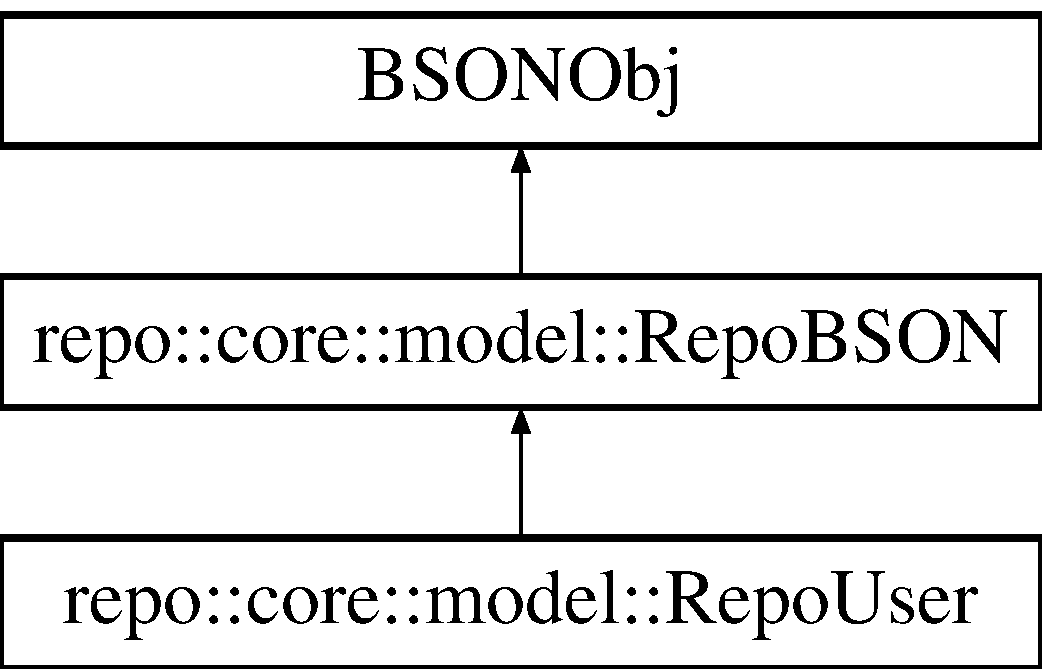
\includegraphics[height=3.000000cm]{classrepo_1_1core_1_1model_1_1_repo_user}
\end{center}
\end{figure}
\subsection*{Classes}
\begin{DoxyCompactItemize}
\item 
struct \hyperlink{structrepo_1_1core_1_1model_1_1_repo_user_1_1_subscription_info}{Subscription\+Info}
\end{DoxyCompactItemize}
\subsection*{Public Member Functions}
\begin{DoxyCompactItemize}
\item 
\hypertarget{classrepo_1_1core_1_1model_1_1_repo_user_aea1084a6836596ae2d6b27659c16414a}{}{\bfseries Repo\+User} (\hyperlink{classrepo_1_1core_1_1model_1_1_repo_b_s_o_n}{Repo\+B\+S\+O\+N} bson)\label{classrepo_1_1core_1_1model_1_1_repo_user_aea1084a6836596ae2d6b27659c16414a}

\item 
\hyperlink{classrepo_1_1core_1_1model_1_1_repo_user}{Repo\+User} \hyperlink{classrepo_1_1core_1_1model_1_1_repo_user_a978b5e38fa9b11b40ecd22f16e9cebc4}{clone\+And\+Add\+Role} (const std\+::string \&db\+Name, const std\+::string \&role) const 
\item 
\hyperlink{classrepo_1_1core_1_1model_1_1_repo_user}{Repo\+User} \hyperlink{classrepo_1_1core_1_1model_1_1_repo_user_a2cdeca59b63e766e326df7b7c3c759dd}{clone\+And\+Merge\+User\+Info} (const \hyperlink{classrepo_1_1core_1_1model_1_1_repo_user}{Repo\+User} \&new\+User\+Info) const 
\item 
\hyperlink{classrepo_1_1core_1_1model_1_1_repo_user}{Repo\+User} \hyperlink{classrepo_1_1core_1_1model_1_1_repo_user_a90a5c1918e73e66d3b23614e0696f00d}{clone\+And\+Update\+License\+Count} (const int \&diff, const int64\+\_\+t exp\+Date=-\/1) const 
\item 
\hypertarget{classrepo_1_1core_1_1model_1_1_repo_user_a8a71e9f1c1831f78eec3334e86538480}{}\hyperlink{classrepo_1_1core_1_1model_1_1_repo_user}{Repo\+User} {\bfseries clone\+And\+Update\+Subscriptions} (const std\+::vector$<$ \hyperlink{structrepo_1_1core_1_1model_1_1_repo_user_1_1_subscription_info}{Subscription\+Info} $>$ \&subs) const \label{classrepo_1_1core_1_1model_1_1_repo_user_a8a71e9f1c1831f78eec3334e86538480}

\item 
std\+::list$<$ std\+::pair$<$ std\+::string, std\+::string $>$ $>$ \hyperlink{classrepo_1_1core_1_1model_1_1_repo_user_a0b7fc82e2b6fbdc20d35716f1fe728ec}{get\+A\+P\+I\+Keys\+List} () const 
\item 
std\+::vector$<$ char $>$ \hyperlink{classrepo_1_1core_1_1model_1_1_repo_user_a3d74ec156cfbe972b29024a44eb40d1d}{get\+Avatar\+As\+Raw\+Data} () const 
\item 
std\+::string \hyperlink{classrepo_1_1core_1_1model_1_1_repo_user_ae9ad66fb853addbd37b73105018b25da}{get\+Cleartext\+Password} () const 
\item 
\hyperlink{classrepo_1_1core_1_1model_1_1_repo_b_s_o_n}{Repo\+B\+S\+O\+N} \hyperlink{classrepo_1_1core_1_1model_1_1_repo_user_ab1042e8a4bb197795dcd42ecca44e770}{get\+Custom\+Data\+B\+S\+O\+N} () const 
\item 
\hyperlink{classrepo_1_1core_1_1model_1_1_repo_b_s_o_n}{Repo\+B\+S\+O\+N} \hyperlink{classrepo_1_1core_1_1model_1_1_repo_user_adf71588560ad5d318f12db604ce1762a}{get\+Roles\+B\+S\+O\+N} () const 
\item 
std\+::string \hyperlink{classrepo_1_1core_1_1model_1_1_repo_user_a3f010f00fdf8880e88d786a697832840}{get\+First\+Name} () const 
\item 
std\+::string \hyperlink{classrepo_1_1core_1_1model_1_1_repo_user_ab6fca4716968d3bff91c517092b471a8}{get\+Last\+Name} () const 
\item 
std\+::string \hyperlink{classrepo_1_1core_1_1model_1_1_repo_user_a60eff8abee2614b2ff3bad137fad2634}{get\+User\+Name} () const 
\item 
std\+::string \hyperlink{classrepo_1_1core_1_1model_1_1_repo_user_ad4ebb8b43b1b54f8460d2c074fac0d92}{get\+Email} () const 
\item 
std\+::list$<$ std\+::pair$<$ std\+::string, std\+::string $>$ $>$ \hyperlink{classrepo_1_1core_1_1model_1_1_repo_user_ae87706868f82a0e4b1e630e7b0af158d}{get\+License\+Assignment} () const 
\item 
std\+::string \hyperlink{classrepo_1_1core_1_1model_1_1_repo_user_a429fcd98aec55a529c6e5d6a7f56104d}{get\+Password} () const 
\item 
std\+::list$<$ std\+::pair$<$ std\+::string, std\+::string $>$ $>$ \hyperlink{classrepo_1_1core_1_1model_1_1_repo_user_a3ce3188cb264f053f7508f68210b301c}{get\+Roles\+List} () const 
\item 
std\+::vector$<$ \hyperlink{structrepo_1_1core_1_1model_1_1_repo_user_1_1_subscription_info}{Subscription\+Info} $>$ \hyperlink{classrepo_1_1core_1_1model_1_1_repo_user_a252c008f819e4992ae277e99035167a7}{get\+Subscription\+Info} () const 
\item 
uint32\+\_\+t \hyperlink{classrepo_1_1core_1_1model_1_1_repo_user_a6a1396bb826507640c817a87db045608}{get\+N\+Collaborators} () const 
\item 
double \hyperlink{classrepo_1_1core_1_1model_1_1_repo_user_ab2eca743fef5572c5eec150c5e60262f}{get\+Quota} () const 
\end{DoxyCompactItemize}
\subsection*{Static Public Member Functions}
\begin{DoxyCompactItemize}
\item 
static \hyperlink{structrepo_1_1core_1_1model_1_1_repo_user_1_1_subscription_info}{Subscription\+Info} \hyperlink{classrepo_1_1core_1_1model_1_1_repo_user_a5ce1dc8d8b741324d0d2ce5c637f7265}{create\+Default\+Sub} (const int64\+\_\+t \&expire\+T\+S=-\/1)
\end{DoxyCompactItemize}
\subsection*{Additional Inherited Members}


\subsection{Member Function Documentation}
\hypertarget{classrepo_1_1core_1_1model_1_1_repo_user_a978b5e38fa9b11b40ecd22f16e9cebc4}{}\index{repo\+::core\+::model\+::\+Repo\+User@{repo\+::core\+::model\+::\+Repo\+User}!clone\+And\+Add\+Role@{clone\+And\+Add\+Role}}
\index{clone\+And\+Add\+Role@{clone\+And\+Add\+Role}!repo\+::core\+::model\+::\+Repo\+User@{repo\+::core\+::model\+::\+Repo\+User}}
\subsubsection[{clone\+And\+Add\+Role}]{\setlength{\rightskip}{0pt plus 5cm}{\bf Repo\+User} Repo\+User\+::clone\+And\+Add\+Role (
\begin{DoxyParamCaption}
\item[{const std\+::string \&}]{db\+Name, }
\item[{const std\+::string \&}]{role}
\end{DoxyParamCaption}
) const}\label{classrepo_1_1core_1_1model_1_1_repo_user_a978b5e38fa9b11b40ecd22f16e9cebc4}
Clone and add roles into this use bson 
\begin{DoxyParams}{Parameters}
{\em db\+Name} & name of the database for the role \\
\hline
{\em role} & name of the role \\
\hline
\end{DoxyParams}
\begin{DoxyReturn}{Returns}
returns a cloned repo\+User bson with role added 
\end{DoxyReturn}
\hypertarget{classrepo_1_1core_1_1model_1_1_repo_user_a2cdeca59b63e766e326df7b7c3c759dd}{}\index{repo\+::core\+::model\+::\+Repo\+User@{repo\+::core\+::model\+::\+Repo\+User}!clone\+And\+Merge\+User\+Info@{clone\+And\+Merge\+User\+Info}}
\index{clone\+And\+Merge\+User\+Info@{clone\+And\+Merge\+User\+Info}!repo\+::core\+::model\+::\+Repo\+User@{repo\+::core\+::model\+::\+Repo\+User}}
\subsubsection[{clone\+And\+Merge\+User\+Info}]{\setlength{\rightskip}{0pt plus 5cm}{\bf Repo\+User} Repo\+User\+::clone\+And\+Merge\+User\+Info (
\begin{DoxyParamCaption}
\item[{const {\bf Repo\+User} \&}]{new\+User\+Info}
\end{DoxyParamCaption}
) const}\label{classrepo_1_1core_1_1model_1_1_repo_user_a2cdeca59b63e766e326df7b7c3c759dd}
Clone and merge new user info into the existing info  new info that needs ot be added/updated \begin{DoxyReturn}{Returns}
returns a new user with fields updated 
\end{DoxyReturn}
\hypertarget{classrepo_1_1core_1_1model_1_1_repo_user_a90a5c1918e73e66d3b23614e0696f00d}{}\index{repo\+::core\+::model\+::\+Repo\+User@{repo\+::core\+::model\+::\+Repo\+User}!clone\+And\+Update\+License\+Count@{clone\+And\+Update\+License\+Count}}
\index{clone\+And\+Update\+License\+Count@{clone\+And\+Update\+License\+Count}!repo\+::core\+::model\+::\+Repo\+User@{repo\+::core\+::model\+::\+Repo\+User}}
\subsubsection[{clone\+And\+Update\+License\+Count}]{\setlength{\rightskip}{0pt plus 5cm}{\bf Repo\+User} Repo\+User\+::clone\+And\+Update\+License\+Count (
\begin{DoxyParamCaption}
\item[{const int \&}]{diff, }
\item[{const int64\+\_\+t}]{exp\+Date = {\ttfamily -\/1}}
\end{DoxyParamCaption}
) const}\label{classrepo_1_1core_1_1model_1_1_repo_user_a90a5c1918e73e66d3b23614e0696f00d}
Clone and increase/decrease license count if diff is positive, it will add new default licenses If we are trying to decrease n licenses, there has to be n unassigned, active licenses. 
\begin{DoxyParams}{Parameters}
{\em diff} & the increase or decrease of license (-\/1 to remove 1, 1 to add 1) \\
\hline
{\em exp\+Date} & specify the expiry date of the license (default is -\/1, which never expires) \\
\hline
\end{DoxyParams}
\begin{DoxyReturn}{Returns}
a cloned version of repo\+User with subscription information updated 
\end{DoxyReturn}
\hypertarget{classrepo_1_1core_1_1model_1_1_repo_user_a5ce1dc8d8b741324d0d2ce5c637f7265}{}\index{repo\+::core\+::model\+::\+Repo\+User@{repo\+::core\+::model\+::\+Repo\+User}!create\+Default\+Sub@{create\+Default\+Sub}}
\index{create\+Default\+Sub@{create\+Default\+Sub}!repo\+::core\+::model\+::\+Repo\+User@{repo\+::core\+::model\+::\+Repo\+User}}
\subsubsection[{create\+Default\+Sub}]{\setlength{\rightskip}{0pt plus 5cm}{\bf Repo\+User\+::\+Subscription\+Info} Repo\+User\+::create\+Default\+Sub (
\begin{DoxyParamCaption}
\item[{const int64\+\_\+t \&}]{expire\+T\+S = {\ttfamily -\/1}}
\end{DoxyParamCaption}
)\hspace{0.3cm}{\ttfamily [static]}}\label{classrepo_1_1core_1_1model_1_1_repo_user_a5ce1dc8d8b741324d0d2ce5c637f7265}
Generate a default subscription \hypertarget{classrepo_1_1core_1_1model_1_1_repo_user_a0b7fc82e2b6fbdc20d35716f1fe728ec}{}\index{repo\+::core\+::model\+::\+Repo\+User@{repo\+::core\+::model\+::\+Repo\+User}!get\+A\+P\+I\+Keys\+List@{get\+A\+P\+I\+Keys\+List}}
\index{get\+A\+P\+I\+Keys\+List@{get\+A\+P\+I\+Keys\+List}!repo\+::core\+::model\+::\+Repo\+User@{repo\+::core\+::model\+::\+Repo\+User}}
\subsubsection[{get\+A\+P\+I\+Keys\+List}]{\setlength{\rightskip}{0pt plus 5cm}std\+::list$<$ std\+::pair$<$ std\+::string, std\+::string $>$ $>$ Repo\+User\+::get\+A\+P\+I\+Keys\+List (
\begin{DoxyParamCaption}
{}
\end{DoxyParamCaption}
) const}\label{classrepo_1_1core_1_1model_1_1_repo_user_a0b7fc82e2b6fbdc20d35716f1fe728ec}
-\/-\/-\/------ Convenience functions -\/-\/-\/-\/-\/------ Get all api keys associated with this user as a list of (label, key) pairs \begin{DoxyReturn}{Returns}
returns a list of label,key pairs 
\end{DoxyReturn}
\hypertarget{classrepo_1_1core_1_1model_1_1_repo_user_a3d74ec156cfbe972b29024a44eb40d1d}{}\index{repo\+::core\+::model\+::\+Repo\+User@{repo\+::core\+::model\+::\+Repo\+User}!get\+Avatar\+As\+Raw\+Data@{get\+Avatar\+As\+Raw\+Data}}
\index{get\+Avatar\+As\+Raw\+Data@{get\+Avatar\+As\+Raw\+Data}!repo\+::core\+::model\+::\+Repo\+User@{repo\+::core\+::model\+::\+Repo\+User}}
\subsubsection[{get\+Avatar\+As\+Raw\+Data}]{\setlength{\rightskip}{0pt plus 5cm}std\+::vector$<$ char $>$ Repo\+User\+::get\+Avatar\+As\+Raw\+Data (
\begin{DoxyParamCaption}
{}
\end{DoxyParamCaption}
) const}\label{classrepo_1_1core_1_1model_1_1_repo_user_a3d74ec156cfbe972b29024a44eb40d1d}
Get avatar image as a vector of char \begin{DoxyReturn}{Returns}
returns a vector of char representing the binary image 
\end{DoxyReturn}
\hypertarget{classrepo_1_1core_1_1model_1_1_repo_user_ae9ad66fb853addbd37b73105018b25da}{}\index{repo\+::core\+::model\+::\+Repo\+User@{repo\+::core\+::model\+::\+Repo\+User}!get\+Cleartext\+Password@{get\+Cleartext\+Password}}
\index{get\+Cleartext\+Password@{get\+Cleartext\+Password}!repo\+::core\+::model\+::\+Repo\+User@{repo\+::core\+::model\+::\+Repo\+User}}
\subsubsection[{get\+Cleartext\+Password}]{\setlength{\rightskip}{0pt plus 5cm}std\+::string Repo\+User\+::get\+Cleartext\+Password (
\begin{DoxyParamCaption}
{}
\end{DoxyParamCaption}
) const}\label{classrepo_1_1core_1_1model_1_1_repo_user_ae9ad66fb853addbd37b73105018b25da}
Get the clear text password of the user \begin{DoxyReturn}{Returns}
returns the clear text password 
\end{DoxyReturn}
\hypertarget{classrepo_1_1core_1_1model_1_1_repo_user_ab1042e8a4bb197795dcd42ecca44e770}{}\index{repo\+::core\+::model\+::\+Repo\+User@{repo\+::core\+::model\+::\+Repo\+User}!get\+Custom\+Data\+B\+S\+O\+N@{get\+Custom\+Data\+B\+S\+O\+N}}
\index{get\+Custom\+Data\+B\+S\+O\+N@{get\+Custom\+Data\+B\+S\+O\+N}!repo\+::core\+::model\+::\+Repo\+User@{repo\+::core\+::model\+::\+Repo\+User}}
\subsubsection[{get\+Custom\+Data\+B\+S\+O\+N}]{\setlength{\rightskip}{0pt plus 5cm}{\bf Repo\+B\+S\+O\+N} Repo\+User\+::get\+Custom\+Data\+B\+S\+O\+N (
\begin{DoxyParamCaption}
{}
\end{DoxyParamCaption}
) const}\label{classrepo_1_1core_1_1model_1_1_repo_user_ab1042e8a4bb197795dcd42ecca44e770}
Get the custom data within the user bson as a bson \begin{DoxyReturn}{Returns}
returns a bson with custom data in it 
\end{DoxyReturn}
\hypertarget{classrepo_1_1core_1_1model_1_1_repo_user_ad4ebb8b43b1b54f8460d2c074fac0d92}{}\index{repo\+::core\+::model\+::\+Repo\+User@{repo\+::core\+::model\+::\+Repo\+User}!get\+Email@{get\+Email}}
\index{get\+Email@{get\+Email}!repo\+::core\+::model\+::\+Repo\+User@{repo\+::core\+::model\+::\+Repo\+User}}
\subsubsection[{get\+Email}]{\setlength{\rightskip}{0pt plus 5cm}std\+::string repo\+::core\+::model\+::\+Repo\+User\+::get\+Email (
\begin{DoxyParamCaption}
{}
\end{DoxyParamCaption}
) const\hspace{0.3cm}{\ttfamily [inline]}}\label{classrepo_1_1core_1_1model_1_1_repo_user_ad4ebb8b43b1b54f8460d2c074fac0d92}
Get the email of this user \begin{DoxyReturn}{Returns}
returns email of the user, empty string if none 
\end{DoxyReturn}
\hypertarget{classrepo_1_1core_1_1model_1_1_repo_user_a3f010f00fdf8880e88d786a697832840}{}\index{repo\+::core\+::model\+::\+Repo\+User@{repo\+::core\+::model\+::\+Repo\+User}!get\+First\+Name@{get\+First\+Name}}
\index{get\+First\+Name@{get\+First\+Name}!repo\+::core\+::model\+::\+Repo\+User@{repo\+::core\+::model\+::\+Repo\+User}}
\subsubsection[{get\+First\+Name}]{\setlength{\rightskip}{0pt plus 5cm}std\+::string repo\+::core\+::model\+::\+Repo\+User\+::get\+First\+Name (
\begin{DoxyParamCaption}
{}
\end{DoxyParamCaption}
) const\hspace{0.3cm}{\ttfamily [inline]}}\label{classrepo_1_1core_1_1model_1_1_repo_user_a3f010f00fdf8880e88d786a697832840}
Get the first name of this user \begin{DoxyReturn}{Returns}
returns first name of the user, empty string if none 
\end{DoxyReturn}
\hypertarget{classrepo_1_1core_1_1model_1_1_repo_user_ab6fca4716968d3bff91c517092b471a8}{}\index{repo\+::core\+::model\+::\+Repo\+User@{repo\+::core\+::model\+::\+Repo\+User}!get\+Last\+Name@{get\+Last\+Name}}
\index{get\+Last\+Name@{get\+Last\+Name}!repo\+::core\+::model\+::\+Repo\+User@{repo\+::core\+::model\+::\+Repo\+User}}
\subsubsection[{get\+Last\+Name}]{\setlength{\rightskip}{0pt plus 5cm}std\+::string repo\+::core\+::model\+::\+Repo\+User\+::get\+Last\+Name (
\begin{DoxyParamCaption}
{}
\end{DoxyParamCaption}
) const\hspace{0.3cm}{\ttfamily [inline]}}\label{classrepo_1_1core_1_1model_1_1_repo_user_ab6fca4716968d3bff91c517092b471a8}
Get the last name of this user \begin{DoxyReturn}{Returns}
returns last name of the user, empty string if none 
\end{DoxyReturn}
\hypertarget{classrepo_1_1core_1_1model_1_1_repo_user_ae87706868f82a0e4b1e630e7b0af158d}{}\index{repo\+::core\+::model\+::\+Repo\+User@{repo\+::core\+::model\+::\+Repo\+User}!get\+License\+Assignment@{get\+License\+Assignment}}
\index{get\+License\+Assignment@{get\+License\+Assignment}!repo\+::core\+::model\+::\+Repo\+User@{repo\+::core\+::model\+::\+Repo\+User}}
\subsubsection[{get\+License\+Assignment}]{\setlength{\rightskip}{0pt plus 5cm}std\+::list$<$ std\+::pair$<$ std\+::string, std\+::string $>$ $>$ Repo\+User\+::get\+License\+Assignment (
\begin{DoxyParamCaption}
{}
\end{DoxyParamCaption}
) const}\label{classrepo_1_1core_1_1model_1_1_repo_user_ae87706868f82a0e4b1e630e7b0af158d}
Get information on how the licenses are assigned If the license isn\textquotesingle{}t assigned, returns an empty string \begin{DoxyReturn}{Returns}
returns a list of pair \{license plan name, assignment\} 
\end{DoxyReturn}
\hypertarget{classrepo_1_1core_1_1model_1_1_repo_user_a6a1396bb826507640c817a87db045608}{}\index{repo\+::core\+::model\+::\+Repo\+User@{repo\+::core\+::model\+::\+Repo\+User}!get\+N\+Collaborators@{get\+N\+Collaborators}}
\index{get\+N\+Collaborators@{get\+N\+Collaborators}!repo\+::core\+::model\+::\+Repo\+User@{repo\+::core\+::model\+::\+Repo\+User}}
\subsubsection[{get\+N\+Collaborators}]{\setlength{\rightskip}{0pt plus 5cm}uint32\+\_\+t Repo\+User\+::get\+N\+Collaborators (
\begin{DoxyParamCaption}
{}
\end{DoxyParamCaption}
) const}\label{classrepo_1_1core_1_1model_1_1_repo_user_a6a1396bb826507640c817a87db045608}
Get the current collaborator limit of the user \begin{DoxyReturn}{Returns}
returns the number of collaborators available to the user 
\end{DoxyReturn}
\hypertarget{classrepo_1_1core_1_1model_1_1_repo_user_a429fcd98aec55a529c6e5d6a7f56104d}{}\index{repo\+::core\+::model\+::\+Repo\+User@{repo\+::core\+::model\+::\+Repo\+User}!get\+Password@{get\+Password}}
\index{get\+Password@{get\+Password}!repo\+::core\+::model\+::\+Repo\+User@{repo\+::core\+::model\+::\+Repo\+User}}
\subsubsection[{get\+Password}]{\setlength{\rightskip}{0pt plus 5cm}std\+::string Repo\+User\+::get\+Password (
\begin{DoxyParamCaption}
{}
\end{DoxyParamCaption}
) const}\label{classrepo_1_1core_1_1model_1_1_repo_user_a429fcd98aec55a529c6e5d6a7f56104d}
Get the password of this user \begin{DoxyReturn}{Returns}
returns masked password of the user 
\end{DoxyReturn}
\hypertarget{classrepo_1_1core_1_1model_1_1_repo_user_ab2eca743fef5572c5eec150c5e60262f}{}\index{repo\+::core\+::model\+::\+Repo\+User@{repo\+::core\+::model\+::\+Repo\+User}!get\+Quota@{get\+Quota}}
\index{get\+Quota@{get\+Quota}!repo\+::core\+::model\+::\+Repo\+User@{repo\+::core\+::model\+::\+Repo\+User}}
\subsubsection[{get\+Quota}]{\setlength{\rightskip}{0pt plus 5cm}double Repo\+User\+::get\+Quota (
\begin{DoxyParamCaption}
{}
\end{DoxyParamCaption}
) const}\label{classrepo_1_1core_1_1model_1_1_repo_user_ab2eca743fef5572c5eec150c5e60262f}
Get the current quota of the user \begin{DoxyReturn}{Returns}
returns the quota available to the user 
\end{DoxyReturn}
\hypertarget{classrepo_1_1core_1_1model_1_1_repo_user_adf71588560ad5d318f12db604ce1762a}{}\index{repo\+::core\+::model\+::\+Repo\+User@{repo\+::core\+::model\+::\+Repo\+User}!get\+Roles\+B\+S\+O\+N@{get\+Roles\+B\+S\+O\+N}}
\index{get\+Roles\+B\+S\+O\+N@{get\+Roles\+B\+S\+O\+N}!repo\+::core\+::model\+::\+Repo\+User@{repo\+::core\+::model\+::\+Repo\+User}}
\subsubsection[{get\+Roles\+B\+S\+O\+N}]{\setlength{\rightskip}{0pt plus 5cm}{\bf Repo\+B\+S\+O\+N} Repo\+User\+::get\+Roles\+B\+S\+O\+N (
\begin{DoxyParamCaption}
{}
\end{DoxyParamCaption}
) const}\label{classrepo_1_1core_1_1model_1_1_repo_user_adf71588560ad5d318f12db604ce1762a}
Get the roles within the user bson as a bson \begin{DoxyReturn}{Returns}
returns a bson with roles in it 
\end{DoxyReturn}
\hypertarget{classrepo_1_1core_1_1model_1_1_repo_user_a3ce3188cb264f053f7508f68210b301c}{}\index{repo\+::core\+::model\+::\+Repo\+User@{repo\+::core\+::model\+::\+Repo\+User}!get\+Roles\+List@{get\+Roles\+List}}
\index{get\+Roles\+List@{get\+Roles\+List}!repo\+::core\+::model\+::\+Repo\+User@{repo\+::core\+::model\+::\+Repo\+User}}
\subsubsection[{get\+Roles\+List}]{\setlength{\rightskip}{0pt plus 5cm}std\+::list$<$ std\+::pair$<$ std\+::string, std\+::string $>$ $>$ Repo\+User\+::get\+Roles\+List (
\begin{DoxyParamCaption}
{}
\end{DoxyParamCaption}
) const}\label{classrepo_1_1core_1_1model_1_1_repo_user_a3ce3188cb264f053f7508f68210b301c}
Get list of roles \begin{DoxyReturn}{Returns}
returns a vector of string pairs (database, roles) 
\end{DoxyReturn}
\hypertarget{classrepo_1_1core_1_1model_1_1_repo_user_a252c008f819e4992ae277e99035167a7}{}\index{repo\+::core\+::model\+::\+Repo\+User@{repo\+::core\+::model\+::\+Repo\+User}!get\+Subscription\+Info@{get\+Subscription\+Info}}
\index{get\+Subscription\+Info@{get\+Subscription\+Info}!repo\+::core\+::model\+::\+Repo\+User@{repo\+::core\+::model\+::\+Repo\+User}}
\subsubsection[{get\+Subscription\+Info}]{\setlength{\rightskip}{0pt plus 5cm}std\+::vector$<$ {\bf Repo\+User\+::\+Subscription\+Info} $>$ Repo\+User\+::get\+Subscription\+Info (
\begin{DoxyParamCaption}
{}
\end{DoxyParamCaption}
) const}\label{classrepo_1_1core_1_1model_1_1_repo_user_a252c008f819e4992ae277e99035167a7}
Get list of subscription info \begin{DoxyReturn}{Returns}
returns a vector of subscription info 
\end{DoxyReturn}
\hypertarget{classrepo_1_1core_1_1model_1_1_repo_user_a60eff8abee2614b2ff3bad137fad2634}{}\index{repo\+::core\+::model\+::\+Repo\+User@{repo\+::core\+::model\+::\+Repo\+User}!get\+User\+Name@{get\+User\+Name}}
\index{get\+User\+Name@{get\+User\+Name}!repo\+::core\+::model\+::\+Repo\+User@{repo\+::core\+::model\+::\+Repo\+User}}
\subsubsection[{get\+User\+Name}]{\setlength{\rightskip}{0pt plus 5cm}std\+::string repo\+::core\+::model\+::\+Repo\+User\+::get\+User\+Name (
\begin{DoxyParamCaption}
{}
\end{DoxyParamCaption}
) const\hspace{0.3cm}{\ttfamily [inline]}}\label{classrepo_1_1core_1_1model_1_1_repo_user_a60eff8abee2614b2ff3bad137fad2634}
Get the username from this user \begin{DoxyReturn}{Returns}
returns user name of the user, empty string if none 
\end{DoxyReturn}


The documentation for this class was generated from the following files\+:\begin{DoxyCompactItemize}
\item 
C\+:/\+Users/\+Carmen/3\+D Repo/\+Repo/3drepobouncer/bouncer/src/repo/core/model/bson/repo\+\_\+bson\+\_\+user.\+h\item 
C\+:/\+Users/\+Carmen/3\+D Repo/\+Repo/3drepobouncer/bouncer/src/repo/core/model/bson/repo\+\_\+bson\+\_\+user.\+cpp\end{DoxyCompactItemize}

\hypertarget{struct_repo_u_u_i_d_hasher}{}\section{Repo\+U\+U\+I\+D\+Hasher Struct Reference}
\label{struct_repo_u_u_i_d_hasher}\index{Repo\+U\+U\+I\+D\+Hasher@{Repo\+U\+U\+I\+D\+Hasher}}
\subsection*{Public Member Functions}
\begin{DoxyCompactItemize}
\item 
\hypertarget{struct_repo_u_u_i_d_hasher_aa4e7aa4aa72ee3d873a30d5d039bb5f4}{}std\+::size\+\_\+t {\bfseries operator()} (const repo\+U\+U\+I\+D \&uid) const \label{struct_repo_u_u_i_d_hasher_aa4e7aa4aa72ee3d873a30d5d039bb5f4}

\end{DoxyCompactItemize}


The documentation for this struct was generated from the following file\+:\begin{DoxyCompactItemize}
\item 
C\+:/\+Users/\+Carmen/3\+D Repo/\+Repo/3drepobouncer/bouncer/src/repo/core/model/repo\+\_\+node\+\_\+utils.\+h\end{DoxyCompactItemize}

\hypertarget{structrepo_1_1core_1_1model_1_1_repo_u_u_i_d_hasher}{}\section{repo\+:\+:core\+:\+:model\+:\+:Repo\+U\+U\+I\+D\+Hasher Struct Reference}
\label{structrepo_1_1core_1_1model_1_1_repo_u_u_i_d_hasher}\index{repo\+::core\+::model\+::\+Repo\+U\+U\+I\+D\+Hasher@{repo\+::core\+::model\+::\+Repo\+U\+U\+I\+D\+Hasher}}
\subsection*{Public Member Functions}
\begin{DoxyCompactItemize}
\item 
\hypertarget{structrepo_1_1core_1_1model_1_1_repo_u_u_i_d_hasher_a5ad0c50eff46364ea58c732b7578b83c}{}std\+::size\+\_\+t {\bfseries operator()} (const repo\+U\+U\+I\+D \&uid) const \label{structrepo_1_1core_1_1model_1_1_repo_u_u_i_d_hasher_a5ad0c50eff46364ea58c732b7578b83c}

\end{DoxyCompactItemize}


The documentation for this struct was generated from the following file\+:\begin{DoxyCompactItemize}
\item 
C\+:/\+Users/\+Carmen/3\+D Repo/\+Repo/3drepobouncer/bouncer/src/repo/core/model/collection/repo\+\_\+scene.\+h\end{DoxyCompactItemize}

\hypertarget{classrepo_1_1core_1_1model_1_1_revision_graph}{}\section{repo\+:\+:core\+:\+:model\+:\+:Revision\+Graph Class Reference}
\label{classrepo_1_1core_1_1model_1_1_revision_graph}\index{repo\+::core\+::model\+::\+Revision\+Graph@{repo\+::core\+::model\+::\+Revision\+Graph}}
Inheritance diagram for repo\+:\+:core\+:\+:model\+:\+:Revision\+Graph\+:\begin{figure}[H]
\begin{center}
\leavevmode
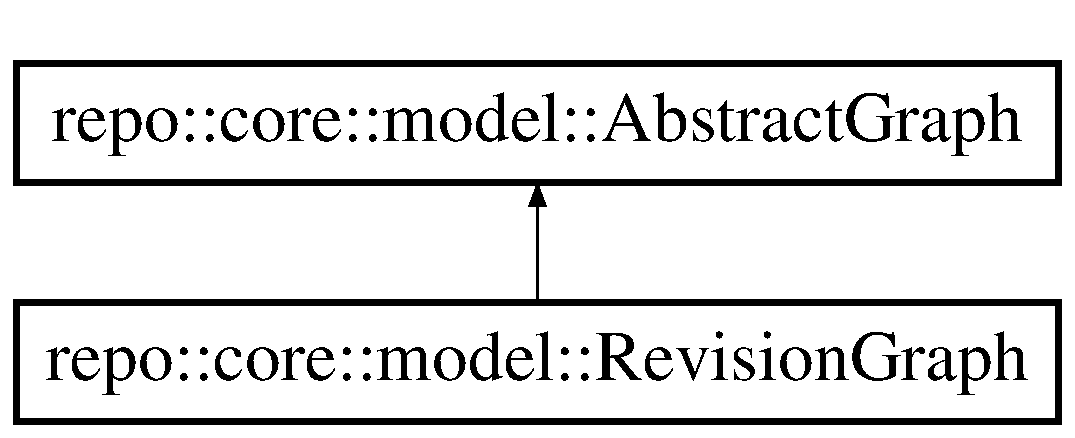
\includegraphics[height=2.000000cm]{classrepo_1_1core_1_1model_1_1_revision_graph}
\end{center}
\end{figure}
\subsection*{Additional Inherited Members}


The documentation for this class was generated from the following files\+:\begin{DoxyCompactItemize}
\item 
C\+:/\+Users/\+Carmen/3\+D Repo/\+Repo/3drepobouncer/bouncer/src/repo/core/model/collection/repo\+\_\+graph\+\_\+revision.\+h\item 
C\+:/\+Users/\+Carmen/3\+D Repo/\+Repo/3drepobouncer/bouncer/src/repo/core/model/collection/repo\+\_\+graph\+\_\+revision.\+cpp\end{DoxyCompactItemize}

\hypertarget{classrepo_1_1core_1_1model_1_1_revision_node}{}\section{repo\+:\+:core\+:\+:model\+:\+:Revision\+Node Class Reference}
\label{classrepo_1_1core_1_1model_1_1_revision_node}\index{repo\+::core\+::model\+::\+Revision\+Node@{repo\+::core\+::model\+::\+Revision\+Node}}
Inheritance diagram for repo\+:\+:core\+:\+:model\+:\+:Revision\+Node\+:\begin{figure}[H]
\begin{center}
\leavevmode
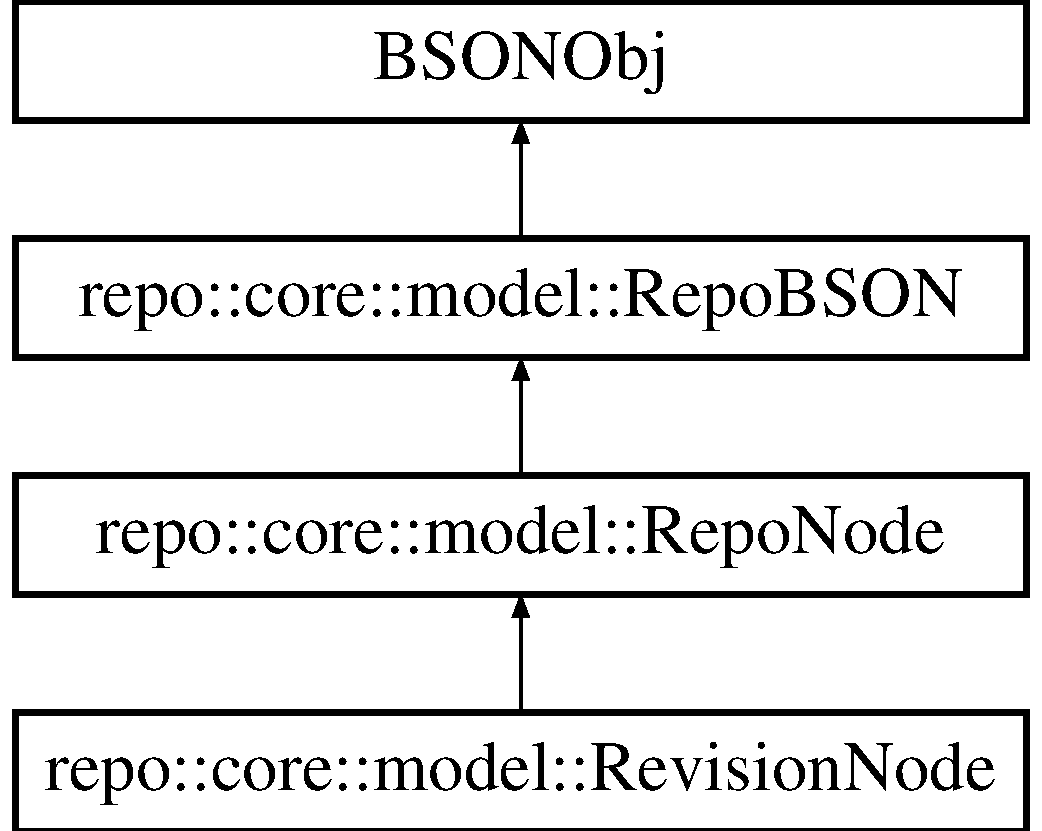
\includegraphics[height=4.000000cm]{classrepo_1_1core_1_1model_1_1_revision_node}
\end{center}
\end{figure}
\subsection*{Public Types}
\begin{DoxyCompactItemize}
\item 
\hypertarget{classrepo_1_1core_1_1model_1_1_revision_node_ae0b95edf7e0e59bce7365ad979c2704a}{}enum {\bfseries Upload\+Status} \{ \\*
{\bfseries C\+O\+M\+P\+L\+E\+T\+E} = 0, 
{\bfseries G\+E\+N\+\_\+\+D\+E\+F\+A\+U\+L\+T} = 1, 
{\bfseries G\+E\+N\+\_\+\+R\+E\+P\+O\+\_\+\+S\+T\+A\+S\+H} = 2, 
{\bfseries G\+E\+N\+\_\+\+W\+E\+B\+\_\+\+S\+T\+A\+S\+H} = 3, 
\\*
{\bfseries G\+E\+N\+\_\+\+S\+E\+L\+\_\+\+T\+R\+E\+E} = 4, 
{\bfseries U\+N\+K\+N\+O\+W\+N} = 5
 \}\label{classrepo_1_1core_1_1model_1_1_revision_node_ae0b95edf7e0e59bce7365ad979c2704a}

\end{DoxyCompactItemize}
\subsection*{Public Member Functions}
\begin{DoxyCompactItemize}
\item 
\hyperlink{classrepo_1_1core_1_1model_1_1_revision_node_ad92597d9731079e4d0bdf690f532e56e}{Revision\+Node} (\hyperlink{classrepo_1_1core_1_1model_1_1_repo_b_s_o_n}{Repo\+B\+S\+O\+N} bson)
\item 
virtual std\+::string \hyperlink{classrepo_1_1core_1_1model_1_1_revision_node_ac597aa317c2516be9f204e43ef896af4}{get\+Type} () const 
\item 
virtual Node\+Type \hyperlink{classrepo_1_1core_1_1model_1_1_revision_node_ae632d941e5a9bc2d8275c53bb1c41805}{get\+Type\+As\+Enum} () const 
\item 
\hyperlink{classrepo_1_1core_1_1model_1_1_revision_node}{Revision\+Node} \hyperlink{classrepo_1_1core_1_1model_1_1_revision_node_afabdf3d38019948f68e331610671583a}{clone\+And\+Update\+Status} (const Upload\+Status \&status) const 
\item 
std\+::string \hyperlink{classrepo_1_1core_1_1model_1_1_revision_node_af5a787130259c6744bcbf90eb7e23d65}{get\+Author} () const 
\item 
std\+::vector$<$ double $>$ \hyperlink{classrepo_1_1core_1_1model_1_1_revision_node_a5990bdfccf6db7f3fdf6167a51fd8f36}{get\+Coord\+Offset} () const 
\item 
std\+::vector$<$ repo\+U\+U\+I\+D $>$ \hyperlink{classrepo_1_1core_1_1model_1_1_revision_node_a90c58bc79e6a209907de191207b5e7fa}{get\+Current\+I\+Ds} () const 
\item 
std\+::string \hyperlink{classrepo_1_1core_1_1model_1_1_revision_node_a955d01925d470a40911b85b432a30c32}{get\+Message} () const 
\item 
std\+::string \hyperlink{classrepo_1_1core_1_1model_1_1_revision_node_aa8c67c1cb49adb80e0a746276cd560c8}{get\+Tag} () const 
\item 
Upload\+Status \hyperlink{classrepo_1_1core_1_1model_1_1_revision_node_ac0a4532dc10c44db48ed2e8a0ae29f30}{get\+Upload\+Status} () const 
\item 
std\+::vector$<$ std\+::string $>$ \hyperlink{classrepo_1_1core_1_1model_1_1_revision_node_a5c51b2bdfb7bbc1b291c4e6e84b46511}{get\+Org\+Files} () const 
\item 
int64\+\_\+t \hyperlink{classrepo_1_1core_1_1model_1_1_revision_node_ac7a14a78c8ab2372026b5f13e1f0e931}{get\+Timestamp\+Int64} () const 
\end{DoxyCompactItemize}
\subsection*{Additional Inherited Members}


\subsection{Constructor \& Destructor Documentation}
\hypertarget{classrepo_1_1core_1_1model_1_1_revision_node_ad92597d9731079e4d0bdf690f532e56e}{}\index{repo\+::core\+::model\+::\+Revision\+Node@{repo\+::core\+::model\+::\+Revision\+Node}!Revision\+Node@{Revision\+Node}}
\index{Revision\+Node@{Revision\+Node}!repo\+::core\+::model\+::\+Revision\+Node@{repo\+::core\+::model\+::\+Revision\+Node}}
\subsubsection[{Revision\+Node}]{\setlength{\rightskip}{0pt plus 5cm}Revision\+Node\+::\+Revision\+Node (
\begin{DoxyParamCaption}
\item[{{\bf Repo\+B\+S\+O\+N}}]{bson}
\end{DoxyParamCaption}
)}\label{classrepo_1_1core_1_1model_1_1_revision_node_ad92597d9731079e4d0bdf690f532e56e}
Constructor Construct a \hyperlink{classrepo_1_1core_1_1model_1_1_repo_node}{Repo\+Node} base on a \hyperlink{classrepo_1_1core_1_1model_1_1_repo_b_s_o_n}{Repo\+B\+S\+O\+N} object 
\begin{DoxyParams}{Parameters}
{\em replicate} & this bson object \\
\hline
\end{DoxyParams}


\subsection{Member Function Documentation}
\hypertarget{classrepo_1_1core_1_1model_1_1_revision_node_afabdf3d38019948f68e331610671583a}{}\index{repo\+::core\+::model\+::\+Revision\+Node@{repo\+::core\+::model\+::\+Revision\+Node}!clone\+And\+Update\+Status@{clone\+And\+Update\+Status}}
\index{clone\+And\+Update\+Status@{clone\+And\+Update\+Status}!repo\+::core\+::model\+::\+Revision\+Node@{repo\+::core\+::model\+::\+Revision\+Node}}
\subsubsection[{clone\+And\+Update\+Status}]{\setlength{\rightskip}{0pt plus 5cm}{\bf Revision\+Node} Revision\+Node\+::clone\+And\+Update\+Status (
\begin{DoxyParamCaption}
\item[{const Upload\+Status \&}]{status}
\end{DoxyParamCaption}
) const}\label{classrepo_1_1core_1_1model_1_1_revision_node_afabdf3d38019948f68e331610671583a}
Update the status flag with the given status N\+O\+T\+E\+: the status flags denotes what it is currently doing not what has been done. e.\+g. G\+E\+N\+\_\+\+D\+E\+F\+A\+U\+L\+T denotes the revision does not have a fully commited default scene graph 
\begin{DoxyParams}{Parameters}
{\em status} & the status to set to \\
\hline
\end{DoxyParams}
\begin{DoxyReturn}{Returns}
returns a clone of this node with updated status flag 
\end{DoxyReturn}
\hypertarget{classrepo_1_1core_1_1model_1_1_revision_node_af5a787130259c6744bcbf90eb7e23d65}{}\index{repo\+::core\+::model\+::\+Revision\+Node@{repo\+::core\+::model\+::\+Revision\+Node}!get\+Author@{get\+Author}}
\index{get\+Author@{get\+Author}!repo\+::core\+::model\+::\+Revision\+Node@{repo\+::core\+::model\+::\+Revision\+Node}}
\subsubsection[{get\+Author}]{\setlength{\rightskip}{0pt plus 5cm}std\+::string Revision\+Node\+::get\+Author (
\begin{DoxyParamCaption}
{}
\end{DoxyParamCaption}
) const}\label{classrepo_1_1core_1_1model_1_1_revision_node_af5a787130259c6744bcbf90eb7e23d65}
-\/-\/-\/------ Convenience functions -\/-\/-\/-\/-\/------ Get the author commited the revision \begin{DoxyReturn}{Returns}
returns a string for message. empty string if none. 
\end{DoxyReturn}
\hypertarget{classrepo_1_1core_1_1model_1_1_revision_node_a5990bdfccf6db7f3fdf6167a51fd8f36}{}\index{repo\+::core\+::model\+::\+Revision\+Node@{repo\+::core\+::model\+::\+Revision\+Node}!get\+Coord\+Offset@{get\+Coord\+Offset}}
\index{get\+Coord\+Offset@{get\+Coord\+Offset}!repo\+::core\+::model\+::\+Revision\+Node@{repo\+::core\+::model\+::\+Revision\+Node}}
\subsubsection[{get\+Coord\+Offset}]{\setlength{\rightskip}{0pt plus 5cm}std\+::vector$<$ double $>$ Revision\+Node\+::get\+Coord\+Offset (
\begin{DoxyParamCaption}
{}
\end{DoxyParamCaption}
) const}\label{classrepo_1_1core_1_1model_1_1_revision_node_a5990bdfccf6db7f3fdf6167a51fd8f36}
Get the offset coordinates to translate the model \begin{DoxyReturn}{Returns}
return a vector of double (size of 3) 
\end{DoxyReturn}
\hypertarget{classrepo_1_1core_1_1model_1_1_revision_node_a90c58bc79e6a209907de191207b5e7fa}{}\index{repo\+::core\+::model\+::\+Revision\+Node@{repo\+::core\+::model\+::\+Revision\+Node}!get\+Current\+I\+Ds@{get\+Current\+I\+Ds}}
\index{get\+Current\+I\+Ds@{get\+Current\+I\+Ds}!repo\+::core\+::model\+::\+Revision\+Node@{repo\+::core\+::model\+::\+Revision\+Node}}
\subsubsection[{get\+Current\+I\+Ds}]{\setlength{\rightskip}{0pt plus 5cm}std\+::vector$<$ repo\+U\+U\+I\+D $>$ Revision\+Node\+::get\+Current\+I\+Ds (
\begin{DoxyParamCaption}
{}
\end{DoxyParamCaption}
) const}\label{classrepo_1_1core_1_1model_1_1_revision_node_a90c58bc79e6a209907de191207b5e7fa}
Get a list of current I\+Ds for this revision \begin{DoxyReturn}{Returns}
returns a vector of unique I\+Ds. 
\end{DoxyReturn}
\hypertarget{classrepo_1_1core_1_1model_1_1_revision_node_a955d01925d470a40911b85b432a30c32}{}\index{repo\+::core\+::model\+::\+Revision\+Node@{repo\+::core\+::model\+::\+Revision\+Node}!get\+Message@{get\+Message}}
\index{get\+Message@{get\+Message}!repo\+::core\+::model\+::\+Revision\+Node@{repo\+::core\+::model\+::\+Revision\+Node}}
\subsubsection[{get\+Message}]{\setlength{\rightskip}{0pt plus 5cm}std\+::string Revision\+Node\+::get\+Message (
\begin{DoxyParamCaption}
{}
\end{DoxyParamCaption}
) const}\label{classrepo_1_1core_1_1model_1_1_revision_node_a955d01925d470a40911b85b432a30c32}
Get a list of I\+Ds of nodes which were Added for this revision \begin{DoxyReturn}{Returns}
returns a vector of shared I\+Ds. Get a list of I\+Ds of nodes which were deleted for this revision 

returns a vector of shared I\+Ds. Get a list of I\+Ds of nodes which were modified for this revision 

returns a vector of shared I\+Ds. Get the message commited with the revision 

returns a string for message. empty string if none. 
\end{DoxyReturn}
\hypertarget{classrepo_1_1core_1_1model_1_1_revision_node_a5c51b2bdfb7bbc1b291c4e6e84b46511}{}\index{repo\+::core\+::model\+::\+Revision\+Node@{repo\+::core\+::model\+::\+Revision\+Node}!get\+Org\+Files@{get\+Org\+Files}}
\index{get\+Org\+Files@{get\+Org\+Files}!repo\+::core\+::model\+::\+Revision\+Node@{repo\+::core\+::model\+::\+Revision\+Node}}
\subsubsection[{get\+Org\+Files}]{\setlength{\rightskip}{0pt plus 5cm}std\+::vector$<$ std\+::string $>$ Revision\+Node\+::get\+Org\+Files (
\begin{DoxyParamCaption}
{}
\end{DoxyParamCaption}
) const}\label{classrepo_1_1core_1_1model_1_1_revision_node_a5c51b2bdfb7bbc1b291c4e6e84b46511}
Get the original file(s) the scene original created from \begin{DoxyReturn}{Returns}
returns a vector of string of files 
\end{DoxyReturn}
\hypertarget{classrepo_1_1core_1_1model_1_1_revision_node_aa8c67c1cb49adb80e0a746276cd560c8}{}\index{repo\+::core\+::model\+::\+Revision\+Node@{repo\+::core\+::model\+::\+Revision\+Node}!get\+Tag@{get\+Tag}}
\index{get\+Tag@{get\+Tag}!repo\+::core\+::model\+::\+Revision\+Node@{repo\+::core\+::model\+::\+Revision\+Node}}
\subsubsection[{get\+Tag}]{\setlength{\rightskip}{0pt plus 5cm}std\+::string Revision\+Node\+::get\+Tag (
\begin{DoxyParamCaption}
{}
\end{DoxyParamCaption}
) const}\label{classrepo_1_1core_1_1model_1_1_revision_node_aa8c67c1cb49adb80e0a746276cd560c8}
Get the tag commited with the revision \begin{DoxyReturn}{Returns}
returns a string for tag. empty string if none. 
\end{DoxyReturn}
\hypertarget{classrepo_1_1core_1_1model_1_1_revision_node_ac7a14a78c8ab2372026b5f13e1f0e931}{}\index{repo\+::core\+::model\+::\+Revision\+Node@{repo\+::core\+::model\+::\+Revision\+Node}!get\+Timestamp\+Int64@{get\+Timestamp\+Int64}}
\index{get\+Timestamp\+Int64@{get\+Timestamp\+Int64}!repo\+::core\+::model\+::\+Revision\+Node@{repo\+::core\+::model\+::\+Revision\+Node}}
\subsubsection[{get\+Timestamp\+Int64}]{\setlength{\rightskip}{0pt plus 5cm}int64\+\_\+t Revision\+Node\+::get\+Timestamp\+Int64 (
\begin{DoxyParamCaption}
{}
\end{DoxyParamCaption}
) const}\label{classrepo_1_1core_1_1model_1_1_revision_node_ac7a14a78c8ab2372026b5f13e1f0e931}
Get the timestamp as int when this revision was commited \begin{DoxyReturn}{Returns}
returns a timestamp 
\end{DoxyReturn}
\hypertarget{classrepo_1_1core_1_1model_1_1_revision_node_ac597aa317c2516be9f204e43ef896af4}{}\index{repo\+::core\+::model\+::\+Revision\+Node@{repo\+::core\+::model\+::\+Revision\+Node}!get\+Type@{get\+Type}}
\index{get\+Type@{get\+Type}!repo\+::core\+::model\+::\+Revision\+Node@{repo\+::core\+::model\+::\+Revision\+Node}}
\subsubsection[{get\+Type}]{\setlength{\rightskip}{0pt plus 5cm}virtual std\+::string repo\+::core\+::model\+::\+Revision\+Node\+::get\+Type (
\begin{DoxyParamCaption}
{}
\end{DoxyParamCaption}
) const\hspace{0.3cm}{\ttfamily [inline]}, {\ttfamily [virtual]}}\label{classrepo_1_1core_1_1model_1_1_revision_node_ac597aa317c2516be9f204e43ef896af4}
Get the type of node \begin{DoxyReturn}{Returns}
returns the type as a string 
\end{DoxyReturn}


Reimplemented from \hyperlink{classrepo_1_1core_1_1model_1_1_repo_node_a4380ba349235b5d9b13b41e41975805e}{repo\+::core\+::model\+::\+Repo\+Node}.

\hypertarget{classrepo_1_1core_1_1model_1_1_revision_node_ae632d941e5a9bc2d8275c53bb1c41805}{}\index{repo\+::core\+::model\+::\+Revision\+Node@{repo\+::core\+::model\+::\+Revision\+Node}!get\+Type\+As\+Enum@{get\+Type\+As\+Enum}}
\index{get\+Type\+As\+Enum@{get\+Type\+As\+Enum}!repo\+::core\+::model\+::\+Revision\+Node@{repo\+::core\+::model\+::\+Revision\+Node}}
\subsubsection[{get\+Type\+As\+Enum}]{\setlength{\rightskip}{0pt plus 5cm}virtual Node\+Type repo\+::core\+::model\+::\+Revision\+Node\+::get\+Type\+As\+Enum (
\begin{DoxyParamCaption}
{}
\end{DoxyParamCaption}
) const\hspace{0.3cm}{\ttfamily [inline]}, {\ttfamily [virtual]}}\label{classrepo_1_1core_1_1model_1_1_revision_node_ae632d941e5a9bc2d8275c53bb1c41805}
Get the type of node as an enum \begin{DoxyReturn}{Returns}
returns type as enum. 
\end{DoxyReturn}


Reimplemented from \hyperlink{classrepo_1_1core_1_1model_1_1_repo_node_ad8d5295248dc9beb0b91efb2ce3b61f4}{repo\+::core\+::model\+::\+Repo\+Node}.

\hypertarget{classrepo_1_1core_1_1model_1_1_revision_node_ac0a4532dc10c44db48ed2e8a0ae29f30}{}\index{repo\+::core\+::model\+::\+Revision\+Node@{repo\+::core\+::model\+::\+Revision\+Node}!get\+Upload\+Status@{get\+Upload\+Status}}
\index{get\+Upload\+Status@{get\+Upload\+Status}!repo\+::core\+::model\+::\+Revision\+Node@{repo\+::core\+::model\+::\+Revision\+Node}}
\subsubsection[{get\+Upload\+Status}]{\setlength{\rightskip}{0pt plus 5cm}Revision\+Node\+::\+Upload\+Status Revision\+Node\+::get\+Upload\+Status (
\begin{DoxyParamCaption}
{}
\end{DoxyParamCaption}
) const}\label{classrepo_1_1core_1_1model_1_1_revision_node_ac0a4532dc10c44db48ed2e8a0ae29f30}
Get the status of the upload for this revision \begin{DoxyReturn}{Returns}
the upload status of the revision 
\end{DoxyReturn}


The documentation for this class was generated from the following files\+:\begin{DoxyCompactItemize}
\item 
C\+:/\+Users/\+Carmen/3\+D Repo/\+Repo/3drepobouncer/bouncer/src/repo/core/model/bson/repo\+\_\+node\+\_\+revision.\+h\item 
C\+:/\+Users/\+Carmen/3\+D Repo/\+Repo/3drepobouncer/bouncer/src/repo/core/model/bson/repo\+\_\+node\+\_\+revision.\+cpp\end{DoxyCompactItemize}

\hypertarget{classrepo_1_1manipulator_1_1modelutility_1_1_scene_cleaner}{}\section{repo\+:\+:manipulator\+:\+:modelutility\+:\+:Scene\+Cleaner Class Reference}
\label{classrepo_1_1manipulator_1_1modelutility_1_1_scene_cleaner}\index{repo\+::manipulator\+::modelutility\+::\+Scene\+Cleaner@{repo\+::manipulator\+::modelutility\+::\+Scene\+Cleaner}}
\subsection*{Public Member Functions}
\begin{DoxyCompactItemize}
\item 
\hyperlink{classrepo_1_1manipulator_1_1modelutility_1_1_scene_cleaner_aee9f7f982c38fdde0ce63788d6ac3e64}{Scene\+Cleaner} (const std\+::string \&db\+Name, const std\+::string \&project\+Name, \hyperlink{classrepo_1_1core_1_1handler_1_1_abstract_database_handler}{repo\+::core\+::handler\+::\+Abstract\+Database\+Handler} $\ast$handler)
\item 
\hypertarget{classrepo_1_1manipulator_1_1modelutility_1_1_scene_cleaner_acad499a9cdffb6f509e1cfb9e8194aff}{}bool {\bfseries execute} ()\label{classrepo_1_1manipulator_1_1modelutility_1_1_scene_cleaner_acad499a9cdffb6f509e1cfb9e8194aff}

\end{DoxyCompactItemize}


\subsection{Constructor \& Destructor Documentation}
\hypertarget{classrepo_1_1manipulator_1_1modelutility_1_1_scene_cleaner_aee9f7f982c38fdde0ce63788d6ac3e64}{}\index{repo\+::manipulator\+::modelutility\+::\+Scene\+Cleaner@{repo\+::manipulator\+::modelutility\+::\+Scene\+Cleaner}!Scene\+Cleaner@{Scene\+Cleaner}}
\index{Scene\+Cleaner@{Scene\+Cleaner}!repo\+::manipulator\+::modelutility\+::\+Scene\+Cleaner@{repo\+::manipulator\+::modelutility\+::\+Scene\+Cleaner}}
\subsubsection[{Scene\+Cleaner}]{\setlength{\rightskip}{0pt plus 5cm}Scene\+Cleaner\+::\+Scene\+Cleaner (
\begin{DoxyParamCaption}
\item[{const std\+::string \&}]{db\+Name, }
\item[{const std\+::string \&}]{project\+Name, }
\item[{{\bf repo\+::core\+::handler\+::\+Abstract\+Database\+Handler} $\ast$}]{handler}
\end{DoxyParamCaption}
)}\label{classrepo_1_1manipulator_1_1modelutility_1_1_scene_cleaner_aee9f7f982c38fdde0ce63788d6ac3e64}
Create a scene cleaner cleans up any incomplete scene information within the database  db\+Name database name 
\begin{DoxyParams}{Parameters}
{\em project\+Name} & project name \\
\hline
{\em handler} & database handler to the database \\
\hline
\end{DoxyParams}


The documentation for this class was generated from the following files\+:\begin{DoxyCompactItemize}
\item 
C\+:/\+Users/\+Carmen/3\+D Repo/\+Repo/3drepobouncer/bouncer/src/repo/manipulator/modelutility/repo\+\_\+scene\+\_\+cleaner.\+h\item 
C\+:/\+Users/\+Carmen/3\+D Repo/\+Repo/3drepobouncer/bouncer/src/repo/manipulator/modelutility/repo\+\_\+scene\+\_\+cleaner.\+cpp\end{DoxyCompactItemize}

\hypertarget{classrepo_1_1manipulator_1_1modelutility_1_1_scene_manager}{}\section{repo\+:\+:manipulator\+:\+:modelutility\+:\+:Scene\+Manager Class Reference}
\label{classrepo_1_1manipulator_1_1modelutility_1_1_scene_manager}\index{repo\+::manipulator\+::modelutility\+::\+Scene\+Manager@{repo\+::manipulator\+::modelutility\+::\+Scene\+Manager}}
\subsection*{Public Member Functions}
\begin{DoxyCompactItemize}
\item 
\hyperlink{classrepo_1_1core_1_1model_1_1_repo_scene}{repo\+::core\+::model\+::\+Repo\+Scene} $\ast$ \hyperlink{classrepo_1_1manipulator_1_1modelutility_1_1_scene_manager_a393159e2171e330dff17c601022b59e6}{fetch\+Scene} (\hyperlink{classrepo_1_1core_1_1handler_1_1_abstract_database_handler}{repo\+::core\+::handler\+::\+Abstract\+Database\+Handler} $\ast$handler, const std\+::string \&database, const std\+::string \&project, const repo\+U\+U\+I\+D \&uuid, const bool \&head\+Revision=true, const bool \&light\+Fetch=false)
\item 
\hypertarget{classrepo_1_1manipulator_1_1modelutility_1_1_scene_manager_a42ef4939c4d06427ba863eb38acd7399}{}\hyperlink{classrepo_1_1core_1_1model_1_1_repo_scene}{repo\+::core\+::model\+::\+Repo\+Scene} $\ast$ {\bfseries fetch\+Scene} (\hyperlink{classrepo_1_1core_1_1handler_1_1_abstract_database_handler}{repo\+::core\+::handler\+::\+Abstract\+Database\+Handler} $\ast$handler, const std\+::string \&database, const std\+::string \&project)\label{classrepo_1_1manipulator_1_1modelutility_1_1_scene_manager_a42ef4939c4d06427ba863eb38acd7399}

\item 
void \hyperlink{classrepo_1_1manipulator_1_1modelutility_1_1_scene_manager_a48727470d70808f4798c88d6ed4537c5}{fetch\+Scene} (\hyperlink{classrepo_1_1core_1_1handler_1_1_abstract_database_handler}{repo\+::core\+::handler\+::\+Abstract\+Database\+Handler} $\ast$handler, \hyperlink{classrepo_1_1core_1_1model_1_1_repo_scene}{repo\+::core\+::model\+::\+Repo\+Scene} $\ast$scene)
\item 
bool \hyperlink{classrepo_1_1manipulator_1_1modelutility_1_1_scene_manager_a6d46d5e7e950bb7fdb7d33dbcb68288b}{generate\+And\+Commit\+Selection\+Tree} (\hyperlink{classrepo_1_1core_1_1model_1_1_repo_scene}{repo\+::core\+::model\+::\+Repo\+Scene} $\ast$scene, \hyperlink{classrepo_1_1core_1_1handler_1_1_abstract_database_handler}{repo\+::core\+::handler\+::\+Abstract\+Database\+Handler} $\ast$handler)
\item 
bool \hyperlink{classrepo_1_1manipulator_1_1modelutility_1_1_scene_manager_a41c0fbd6443b3df78aa922b303963f49}{generate\+Stash\+Graph} (\hyperlink{classrepo_1_1core_1_1model_1_1_repo_scene}{repo\+::core\+::model\+::\+Repo\+Scene} $\ast$scene, \hyperlink{classrepo_1_1core_1_1handler_1_1_abstract_database_handler}{repo\+::core\+::handler\+::\+Abstract\+Database\+Handler} $\ast$handler=nullptr)
\item 
bool \hyperlink{classrepo_1_1manipulator_1_1modelutility_1_1_scene_manager_a56d372073aa4d37c3b2f45d02b930929}{generate\+Web\+View\+Buffers} (\hyperlink{classrepo_1_1core_1_1model_1_1_repo_scene}{repo\+::core\+::model\+::\+Repo\+Scene} $\ast$scene, const repo\+::manipulator\+::modelconvertor\+::\+Web\+Export\+Type \&ex\+Type, \hyperlink{structrepo__web__buffers__t}{repo\+\_\+web\+\_\+buffers\+\_\+t} \&result\+Buffers, \hyperlink{classrepo_1_1core_1_1handler_1_1_abstract_database_handler}{repo\+::core\+::handler\+::\+Abstract\+Database\+Handler} $\ast$handler=nullptr)
\item 
bool \hyperlink{classrepo_1_1manipulator_1_1modelutility_1_1_scene_manager_a58af7cd9d7f5f0b0f080914495b82083}{remove\+Stash\+Graph} (\hyperlink{classrepo_1_1core_1_1model_1_1_repo_scene}{repo\+::core\+::model\+::\+Repo\+Scene} $\ast$scene, \hyperlink{classrepo_1_1core_1_1handler_1_1_abstract_database_handler}{repo\+::core\+::handler\+::\+Abstract\+Database\+Handler} $\ast$handler=nullptr)
\end{DoxyCompactItemize}


\subsection{Member Function Documentation}
\hypertarget{classrepo_1_1manipulator_1_1modelutility_1_1_scene_manager_a393159e2171e330dff17c601022b59e6}{}\index{repo\+::manipulator\+::modelutility\+::\+Scene\+Manager@{repo\+::manipulator\+::modelutility\+::\+Scene\+Manager}!fetch\+Scene@{fetch\+Scene}}
\index{fetch\+Scene@{fetch\+Scene}!repo\+::manipulator\+::modelutility\+::\+Scene\+Manager@{repo\+::manipulator\+::modelutility\+::\+Scene\+Manager}}
\subsubsection[{fetch\+Scene}]{\setlength{\rightskip}{0pt plus 5cm}{\bf repo\+::core\+::model\+::\+Repo\+Scene} $\ast$ Scene\+Manager\+::fetch\+Scene (
\begin{DoxyParamCaption}
\item[{{\bf repo\+::core\+::handler\+::\+Abstract\+Database\+Handler} $\ast$}]{handler, }
\item[{const std\+::string \&}]{database, }
\item[{const std\+::string \&}]{project, }
\item[{const repo\+U\+U\+I\+D \&}]{uuid, }
\item[{const bool \&}]{head\+Revision = {\ttfamily true}, }
\item[{const bool \&}]{light\+Fetch = {\ttfamily false}}
\end{DoxyParamCaption}
)}\label{classrepo_1_1manipulator_1_1modelutility_1_1_scene_manager_a393159e2171e330dff17c601022b59e6}
Retrieve a Repo\+Scene with a specific revision loaded. 
\begin{DoxyParams}{Parameters}
{\em handler} & hander to the database \\
\hline
{\em database} & the database the collection resides in \\
\hline
{\em project} & name of the project \\
\hline
{\em uuid} & if head\+Revision, uuid represents the branch id, otherwise the unique id of the revision branch \\
\hline
{\em head\+Revision} & true if retrieving head revision \\
\hline
{\em light\+Fetch} & fetches only the stash (or scene if stash failed), reduce computation and memory usage (ideal for visualisation only) \\
\hline
\end{DoxyParams}
\begin{DoxyReturn}{Returns}
returns a pointer to a repo\+Scene. 
\end{DoxyReturn}
\hypertarget{classrepo_1_1manipulator_1_1modelutility_1_1_scene_manager_a48727470d70808f4798c88d6ed4537c5}{}\index{repo\+::manipulator\+::modelutility\+::\+Scene\+Manager@{repo\+::manipulator\+::modelutility\+::\+Scene\+Manager}!fetch\+Scene@{fetch\+Scene}}
\index{fetch\+Scene@{fetch\+Scene}!repo\+::manipulator\+::modelutility\+::\+Scene\+Manager@{repo\+::manipulator\+::modelutility\+::\+Scene\+Manager}}
\subsubsection[{fetch\+Scene}]{\setlength{\rightskip}{0pt plus 5cm}void Scene\+Manager\+::fetch\+Scene (
\begin{DoxyParamCaption}
\item[{{\bf repo\+::core\+::handler\+::\+Abstract\+Database\+Handler} $\ast$}]{handler, }
\item[{{\bf repo\+::core\+::model\+::\+Repo\+Scene} $\ast$}]{scene}
\end{DoxyParamCaption}
)}\label{classrepo_1_1manipulator_1_1modelutility_1_1_scene_manager_a48727470d70808f4798c88d6ed4537c5}
Retrieve all Repo\+Scene representations given a partially loaded scene. 
\begin{DoxyParams}{Parameters}
{\em handler} & database handler \\
\hline
{\em scene} & scene to fully load \\
\hline
\end{DoxyParams}
\hypertarget{classrepo_1_1manipulator_1_1modelutility_1_1_scene_manager_a6d46d5e7e950bb7fdb7d33dbcb68288b}{}\index{repo\+::manipulator\+::modelutility\+::\+Scene\+Manager@{repo\+::manipulator\+::modelutility\+::\+Scene\+Manager}!generate\+And\+Commit\+Selection\+Tree@{generate\+And\+Commit\+Selection\+Tree}}
\index{generate\+And\+Commit\+Selection\+Tree@{generate\+And\+Commit\+Selection\+Tree}!repo\+::manipulator\+::modelutility\+::\+Scene\+Manager@{repo\+::manipulator\+::modelutility\+::\+Scene\+Manager}}
\subsubsection[{generate\+And\+Commit\+Selection\+Tree}]{\setlength{\rightskip}{0pt plus 5cm}bool Scene\+Manager\+::generate\+And\+Commit\+Selection\+Tree (
\begin{DoxyParamCaption}
\item[{{\bf repo\+::core\+::model\+::\+Repo\+Scene} $\ast$}]{scene, }
\item[{{\bf repo\+::core\+::handler\+::\+Abstract\+Database\+Handler} $\ast$}]{handler}
\end{DoxyParamCaption}
)}\label{classrepo_1_1manipulator_1_1modelutility_1_1_scene_manager_a6d46d5e7e950bb7fdb7d33dbcb68288b}
Generate and commit scene\textquotesingle{}s selection tree in J\+S\+O\+N format The generated data will be also commited to the database/project set within the scene 
\begin{DoxyParams}{Parameters}
{\em scene} & scene to optimise \\
\hline
{\em handler} & hander to the database \\
\hline
\end{DoxyParams}
\begin{DoxyReturn}{Returns}
return true upon success 
\end{DoxyReturn}
\hypertarget{classrepo_1_1manipulator_1_1modelutility_1_1_scene_manager_a41c0fbd6443b3df78aa922b303963f49}{}\index{repo\+::manipulator\+::modelutility\+::\+Scene\+Manager@{repo\+::manipulator\+::modelutility\+::\+Scene\+Manager}!generate\+Stash\+Graph@{generate\+Stash\+Graph}}
\index{generate\+Stash\+Graph@{generate\+Stash\+Graph}!repo\+::manipulator\+::modelutility\+::\+Scene\+Manager@{repo\+::manipulator\+::modelutility\+::\+Scene\+Manager}}
\subsubsection[{generate\+Stash\+Graph}]{\setlength{\rightskip}{0pt plus 5cm}bool Scene\+Manager\+::generate\+Stash\+Graph (
\begin{DoxyParamCaption}
\item[{{\bf repo\+::core\+::model\+::\+Repo\+Scene} $\ast$}]{scene, }
\item[{{\bf repo\+::core\+::handler\+::\+Abstract\+Database\+Handler} $\ast$}]{handler = {\ttfamily nullptr}}
\end{DoxyParamCaption}
)}\label{classrepo_1_1manipulator_1_1modelutility_1_1_scene_manager_a41c0fbd6443b3df78aa922b303963f49}
Generate a stash graph for the given scene and populate it into the given scene If a databasehandler is given and the scene is revisioned, it will commit the stash to database 
\begin{DoxyParams}{Parameters}
{\em scene} & scene to generate stash graph for \\
\hline
{\em handler} & hander to the database \\
\hline
\end{DoxyParams}
\begin{DoxyReturn}{Returns}
returns true upon success 
\end{DoxyReturn}
\hypertarget{classrepo_1_1manipulator_1_1modelutility_1_1_scene_manager_a56d372073aa4d37c3b2f45d02b930929}{}\index{repo\+::manipulator\+::modelutility\+::\+Scene\+Manager@{repo\+::manipulator\+::modelutility\+::\+Scene\+Manager}!generate\+Web\+View\+Buffers@{generate\+Web\+View\+Buffers}}
\index{generate\+Web\+View\+Buffers@{generate\+Web\+View\+Buffers}!repo\+::manipulator\+::modelutility\+::\+Scene\+Manager@{repo\+::manipulator\+::modelutility\+::\+Scene\+Manager}}
\subsubsection[{generate\+Web\+View\+Buffers}]{\setlength{\rightskip}{0pt plus 5cm}bool Scene\+Manager\+::generate\+Web\+View\+Buffers (
\begin{DoxyParamCaption}
\item[{{\bf repo\+::core\+::model\+::\+Repo\+Scene} $\ast$}]{scene, }
\item[{const repo\+::manipulator\+::modelconvertor\+::\+Web\+Export\+Type \&}]{ex\+Type, }
\item[{{\bf repo\+\_\+web\+\_\+buffers\+\_\+t} \&}]{result\+Buffers, }
\item[{{\bf repo\+::core\+::handler\+::\+Abstract\+Database\+Handler} $\ast$}]{handler = {\ttfamily nullptr}}
\end{DoxyParamCaption}
)}\label{classrepo_1_1manipulator_1_1modelutility_1_1_scene_manager_a56d372073aa4d37c3b2f45d02b930929}
Generate a {\ttfamily ex\+Type} encoding for the given scene if a database handler is provided, it will also commit the buffers into the database This requires the repo stash to have been generated already 
\begin{DoxyParams}{Parameters}
{\em scene} & the scene to generate the src encoding from \\
\hline
{\em ex\+Type} & the type of export it is \\
\hline
\end{DoxyParams}
\begin{DoxyReturn}{Returns}
returns repo\+\_\+web\+\_\+buffers upon success 
\end{DoxyReturn}
\hypertarget{classrepo_1_1manipulator_1_1modelutility_1_1_scene_manager_a58af7cd9d7f5f0b0f080914495b82083}{}\index{repo\+::manipulator\+::modelutility\+::\+Scene\+Manager@{repo\+::manipulator\+::modelutility\+::\+Scene\+Manager}!remove\+Stash\+Graph@{remove\+Stash\+Graph}}
\index{remove\+Stash\+Graph@{remove\+Stash\+Graph}!repo\+::manipulator\+::modelutility\+::\+Scene\+Manager@{repo\+::manipulator\+::modelutility\+::\+Scene\+Manager}}
\subsubsection[{remove\+Stash\+Graph}]{\setlength{\rightskip}{0pt plus 5cm}bool Scene\+Manager\+::remove\+Stash\+Graph (
\begin{DoxyParamCaption}
\item[{{\bf repo\+::core\+::model\+::\+Repo\+Scene} $\ast$}]{scene, }
\item[{{\bf repo\+::core\+::handler\+::\+Abstract\+Database\+Handler} $\ast$}]{handler = {\ttfamily nullptr}}
\end{DoxyParamCaption}
)}\label{classrepo_1_1manipulator_1_1modelutility_1_1_scene_manager_a58af7cd9d7f5f0b0f080914495b82083}
Remove stash graph entry for the given scene Will also remove it from the database should handler exist 
\begin{DoxyParams}{Parameters}
{\em scene} & scene reference to remove stash graph from \\
\hline
{\em handler} & hander to the database \\
\hline
\end{DoxyParams}
\begin{DoxyReturn}{Returns}
returns true upon success 
\end{DoxyReturn}


The documentation for this class was generated from the following files\+:\begin{DoxyCompactItemize}
\item 
C\+:/\+Users/\+Carmen/3\+D Repo/\+Repo/3drepobouncer/bouncer/src/repo/manipulator/modelutility/repo\+\_\+scene\+\_\+manager.\+h\item 
C\+:/\+Users/\+Carmen/3\+D Repo/\+Repo/3drepobouncer/bouncer/src/repo/manipulator/modelutility/repo\+\_\+scene\+\_\+manager.\+cpp\end{DoxyCompactItemize}

\hypertarget{classrepo_1_1manipulator_1_1modelutility_1_1_selection_tree_maker}{}\section{repo\+:\+:manipulator\+:\+:modelutility\+:\+:Selection\+Tree\+Maker Class Reference}
\label{classrepo_1_1manipulator_1_1modelutility_1_1_selection_tree_maker}\index{repo\+::manipulator\+::modelutility\+::\+Selection\+Tree\+Maker@{repo\+::manipulator\+::modelutility\+::\+Selection\+Tree\+Maker}}
\subsection*{Public Member Functions}
\begin{DoxyCompactItemize}
\item 
\hyperlink{classrepo_1_1manipulator_1_1modelutility_1_1_selection_tree_maker_a5998b7384ca939372fff25fb06484f7e}{Selection\+Tree\+Maker} (const \hyperlink{classrepo_1_1core_1_1model_1_1_repo_scene}{repo\+::core\+::model\+::\+Repo\+Scene} $\ast$scene)
\item 
std\+::map$<$ std\+::string, \hyperlink{classrepo_1_1lib_1_1_property_tree}{repo\+::lib\+::\+Property\+Tree} $>$ \hyperlink{classrepo_1_1manipulator_1_1modelutility_1_1_selection_tree_maker_a376c460146f83c4eefb09f1990a32f9c}{get\+Selection\+Tree\+As\+Property\+Tree} () const 
\item 
std\+::map$<$ std\+::string, std\+::vector$<$ uint8\+\_\+t $>$ $>$ \hyperlink{classrepo_1_1manipulator_1_1modelutility_1_1_selection_tree_maker_a4f885f52e0deac5798edc3e74a54704d}{get\+Selection\+Tree\+As\+Buffer} () const 
\end{DoxyCompactItemize}


\subsection{Constructor \& Destructor Documentation}
\hypertarget{classrepo_1_1manipulator_1_1modelutility_1_1_selection_tree_maker_a5998b7384ca939372fff25fb06484f7e}{}\index{repo\+::manipulator\+::modelutility\+::\+Selection\+Tree\+Maker@{repo\+::manipulator\+::modelutility\+::\+Selection\+Tree\+Maker}!Selection\+Tree\+Maker@{Selection\+Tree\+Maker}}
\index{Selection\+Tree\+Maker@{Selection\+Tree\+Maker}!repo\+::manipulator\+::modelutility\+::\+Selection\+Tree\+Maker@{repo\+::manipulator\+::modelutility\+::\+Selection\+Tree\+Maker}}
\subsubsection[{Selection\+Tree\+Maker}]{\setlength{\rightskip}{0pt plus 5cm}Selection\+Tree\+Maker\+::\+Selection\+Tree\+Maker (
\begin{DoxyParamCaption}
\item[{const {\bf repo\+::core\+::model\+::\+Repo\+Scene} $\ast$}]{scene}
\end{DoxyParamCaption}
)}\label{classrepo_1_1manipulator_1_1modelutility_1_1_selection_tree_maker_a5998b7384ca939372fff25fb06484f7e}
Create a selection tree maker. The scene must be a valid pointer with Default graph loaded  scene scene to construct from 

\subsection{Member Function Documentation}
\hypertarget{classrepo_1_1manipulator_1_1modelutility_1_1_selection_tree_maker_a4f885f52e0deac5798edc3e74a54704d}{}\index{repo\+::manipulator\+::modelutility\+::\+Selection\+Tree\+Maker@{repo\+::manipulator\+::modelutility\+::\+Selection\+Tree\+Maker}!get\+Selection\+Tree\+As\+Buffer@{get\+Selection\+Tree\+As\+Buffer}}
\index{get\+Selection\+Tree\+As\+Buffer@{get\+Selection\+Tree\+As\+Buffer}!repo\+::manipulator\+::modelutility\+::\+Selection\+Tree\+Maker@{repo\+::manipulator\+::modelutility\+::\+Selection\+Tree\+Maker}}
\subsubsection[{get\+Selection\+Tree\+As\+Buffer}]{\setlength{\rightskip}{0pt plus 5cm}std\+::map$<$ std\+::string, std\+::vector$<$ uint8\+\_\+t $>$ $>$ Selection\+Tree\+Maker\+::get\+Selection\+Tree\+As\+Buffer (
\begin{DoxyParamCaption}
{}
\end{DoxyParamCaption}
) const}\label{classrepo_1_1manipulator_1_1modelutility_1_1_selection_tree_maker_a4f885f52e0deac5798edc3e74a54704d}
Construct and return the selection tree as a Property Tree As a buffer The method will return an empty tree if the scene is null or the default graph is not loaded. \begin{DoxyReturn}{Returns}
returns the selection tree as a property tree 
\end{DoxyReturn}
\hypertarget{classrepo_1_1manipulator_1_1modelutility_1_1_selection_tree_maker_a376c460146f83c4eefb09f1990a32f9c}{}\index{repo\+::manipulator\+::modelutility\+::\+Selection\+Tree\+Maker@{repo\+::manipulator\+::modelutility\+::\+Selection\+Tree\+Maker}!get\+Selection\+Tree\+As\+Property\+Tree@{get\+Selection\+Tree\+As\+Property\+Tree}}
\index{get\+Selection\+Tree\+As\+Property\+Tree@{get\+Selection\+Tree\+As\+Property\+Tree}!repo\+::manipulator\+::modelutility\+::\+Selection\+Tree\+Maker@{repo\+::manipulator\+::modelutility\+::\+Selection\+Tree\+Maker}}
\subsubsection[{get\+Selection\+Tree\+As\+Property\+Tree}]{\setlength{\rightskip}{0pt plus 5cm}std\+::map$<$ std\+::string, {\bf repo\+::lib\+::\+Property\+Tree} $>$ Selection\+Tree\+Maker\+::get\+Selection\+Tree\+As\+Property\+Tree (
\begin{DoxyParamCaption}
{}
\end{DoxyParamCaption}
) const}\label{classrepo_1_1manipulator_1_1modelutility_1_1_selection_tree_maker_a376c460146f83c4eefb09f1990a32f9c}
Construct and return the selection tree as a Property Tree The method will return an empty tree if the scene is null or the default graph is not loaded. \begin{DoxyReturn}{Returns}
returns the selection tree as a property tree 
\end{DoxyReturn}


The documentation for this class was generated from the following files\+:\begin{DoxyCompactItemize}
\item 
C\+:/\+Users/\+Carmen/3\+D Repo/\+Repo/3drepobouncer/bouncer/src/repo/manipulator/modelutility/repo\+\_\+maker\+\_\+selection\+\_\+tree.\+h\item 
C\+:/\+Users/\+Carmen/3\+D Repo/\+Repo/3drepobouncer/bouncer/src/repo/manipulator/modelutility/repo\+\_\+maker\+\_\+selection\+\_\+tree.\+cpp\end{DoxyCompactItemize}

\hypertarget{classrepo_1_1manipulator_1_1modelconvertor_1_1_s_r_c_model_export}{}\section{repo\+:\+:manipulator\+:\+:modelconvertor\+:\+:S\+R\+C\+Model\+Export Class Reference}
\label{classrepo_1_1manipulator_1_1modelconvertor_1_1_s_r_c_model_export}\index{repo\+::manipulator\+::modelconvertor\+::\+S\+R\+C\+Model\+Export@{repo\+::manipulator\+::modelconvertor\+::\+S\+R\+C\+Model\+Export}}
Inheritance diagram for repo\+:\+:manipulator\+:\+:modelconvertor\+:\+:S\+R\+C\+Model\+Export\+:\begin{figure}[H]
\begin{center}
\leavevmode
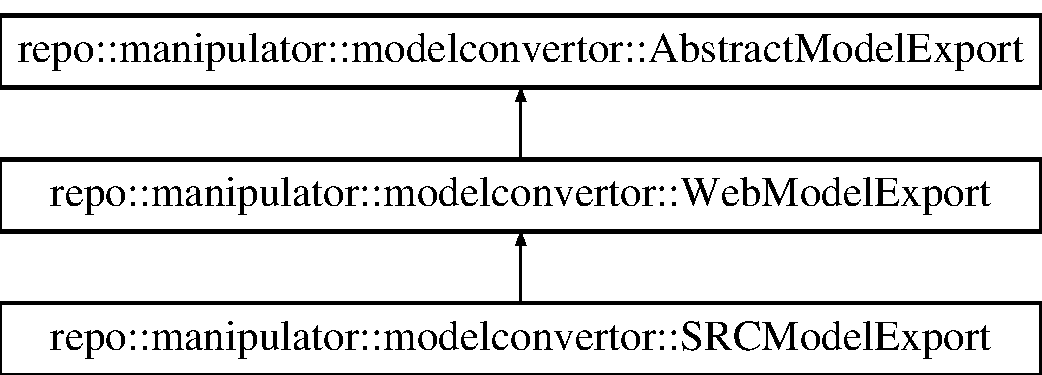
\includegraphics[height=3.000000cm]{classrepo_1_1manipulator_1_1modelconvertor_1_1_s_r_c_model_export}
\end{center}
\end{figure}
\subsection*{Public Member Functions}
\begin{DoxyCompactItemize}
\item 
\hyperlink{classrepo_1_1manipulator_1_1modelconvertor_1_1_s_r_c_model_export_a2207050092968dbbcd7fc403522acca2}{S\+R\+C\+Model\+Export} (const \hyperlink{classrepo_1_1core_1_1model_1_1_repo_scene}{repo\+::core\+::model\+::\+Repo\+Scene} $\ast$scene)
\item 
virtual \hyperlink{classrepo_1_1manipulator_1_1modelconvertor_1_1_s_r_c_model_export_a8f7e17fe1b536103171f884d84a2ea96}{$\sim$\+S\+R\+C\+Model\+Export} ()
\item 
\hyperlink{structrepo__web__buffers__t}{repo\+\_\+web\+\_\+buffers\+\_\+t} \hyperlink{classrepo_1_1manipulator_1_1modelconvertor_1_1_s_r_c_model_export_aabc41be1f3f75ab3cba44df16e40850e}{get\+All\+Files\+Exported\+As\+Buffer} () const 
\end{DoxyCompactItemize}
\subsection*{Additional Inherited Members}


\subsection{Constructor \& Destructor Documentation}
\hypertarget{classrepo_1_1manipulator_1_1modelconvertor_1_1_s_r_c_model_export_a2207050092968dbbcd7fc403522acca2}{}\index{repo\+::manipulator\+::modelconvertor\+::\+S\+R\+C\+Model\+Export@{repo\+::manipulator\+::modelconvertor\+::\+S\+R\+C\+Model\+Export}!S\+R\+C\+Model\+Export@{S\+R\+C\+Model\+Export}}
\index{S\+R\+C\+Model\+Export@{S\+R\+C\+Model\+Export}!repo\+::manipulator\+::modelconvertor\+::\+S\+R\+C\+Model\+Export@{repo\+::manipulator\+::modelconvertor\+::\+S\+R\+C\+Model\+Export}}
\subsubsection[{S\+R\+C\+Model\+Export}]{\setlength{\rightskip}{0pt plus 5cm}S\+R\+C\+Model\+Export\+::\+S\+R\+C\+Model\+Export (
\begin{DoxyParamCaption}
\item[{const {\bf repo\+::core\+::model\+::\+Repo\+Scene} $\ast$}]{scene}
\end{DoxyParamCaption}
)}\label{classrepo_1_1manipulator_1_1modelconvertor_1_1_s_r_c_model_export_a2207050092968dbbcd7fc403522acca2}
Default Constructor, export model with default settings 
\begin{DoxyParams}{Parameters}
{\em scene} & repo scene to convert \\
\hline
\end{DoxyParams}
\hypertarget{classrepo_1_1manipulator_1_1modelconvertor_1_1_s_r_c_model_export_a8f7e17fe1b536103171f884d84a2ea96}{}\index{repo\+::manipulator\+::modelconvertor\+::\+S\+R\+C\+Model\+Export@{repo\+::manipulator\+::modelconvertor\+::\+S\+R\+C\+Model\+Export}!````~S\+R\+C\+Model\+Export@{$\sim$\+S\+R\+C\+Model\+Export}}
\index{````~S\+R\+C\+Model\+Export@{$\sim$\+S\+R\+C\+Model\+Export}!repo\+::manipulator\+::modelconvertor\+::\+S\+R\+C\+Model\+Export@{repo\+::manipulator\+::modelconvertor\+::\+S\+R\+C\+Model\+Export}}
\subsubsection[{$\sim$\+S\+R\+C\+Model\+Export}]{\setlength{\rightskip}{0pt plus 5cm}S\+R\+C\+Model\+Export\+::$\sim$\+S\+R\+C\+Model\+Export (
\begin{DoxyParamCaption}
{}
\end{DoxyParamCaption}
)\hspace{0.3cm}{\ttfamily [virtual]}}\label{classrepo_1_1manipulator_1_1modelconvertor_1_1_s_r_c_model_export_a8f7e17fe1b536103171f884d84a2ea96}
Default Destructor 

\subsection{Member Function Documentation}
\hypertarget{classrepo_1_1manipulator_1_1modelconvertor_1_1_s_r_c_model_export_aabc41be1f3f75ab3cba44df16e40850e}{}\index{repo\+::manipulator\+::modelconvertor\+::\+S\+R\+C\+Model\+Export@{repo\+::manipulator\+::modelconvertor\+::\+S\+R\+C\+Model\+Export}!get\+All\+Files\+Exported\+As\+Buffer@{get\+All\+Files\+Exported\+As\+Buffer}}
\index{get\+All\+Files\+Exported\+As\+Buffer@{get\+All\+Files\+Exported\+As\+Buffer}!repo\+::manipulator\+::modelconvertor\+::\+S\+R\+C\+Model\+Export@{repo\+::manipulator\+::modelconvertor\+::\+S\+R\+C\+Model\+Export}}
\subsubsection[{get\+All\+Files\+Exported\+As\+Buffer}]{\setlength{\rightskip}{0pt plus 5cm}{\bf repo\+\_\+web\+\_\+buffers\+\_\+t} S\+R\+C\+Model\+Export\+::get\+All\+Files\+Exported\+As\+Buffer (
\begin{DoxyParamCaption}
{}
\end{DoxyParamCaption}
) const\hspace{0.3cm}{\ttfamily [virtual]}}\label{classrepo_1_1manipulator_1_1modelconvertor_1_1_s_r_c_model_export_aabc41be1f3f75ab3cba44df16e40850e}
Export all necessary files as buffers \begin{DoxyReturn}{Returns}
returns a repo\+\_\+src\+\_\+export\+\_\+t containing all files needed for this model to be rendered 
\end{DoxyReturn}


Implements \hyperlink{classrepo_1_1manipulator_1_1modelconvertor_1_1_web_model_export_ad9e20343a2e8a21fb9de2e89ba14bf05}{repo\+::manipulator\+::modelconvertor\+::\+Web\+Model\+Export}.



The documentation for this class was generated from the following files\+:\begin{DoxyCompactItemize}
\item 
C\+:/\+Users/\+Carmen/3\+D Repo/\+Repo/3drepobouncer/bouncer/src/repo/manipulator/modelconvertor/export/repo\+\_\+model\+\_\+export\+\_\+src.\+h\item 
C\+:/\+Users/\+Carmen/3\+D Repo/\+Repo/3drepobouncer/bouncer/src/repo/manipulator/modelconvertor/export/repo\+\_\+model\+\_\+export\+\_\+src.\+cpp\end{DoxyCompactItemize}

\hypertarget{structstring_translator}{}\section{string\+Translator Struct Reference}
\label{structstring_translator}\index{string\+Translator@{string\+Translator}}
\subsection*{Public Types}
\begin{DoxyCompactItemize}
\item 
\hypertarget{structstring_translator_af22f5446dd307575b42420692bca063a}{}typedef std\+::string {\bfseries internal\+\_\+type}\label{structstring_translator_af22f5446dd307575b42420692bca063a}

\item 
\hypertarget{structstring_translator_a4cecd98448d6b6971e09ade724f3b41f}{}typedef std\+::string {\bfseries external\+\_\+type}\label{structstring_translator_a4cecd98448d6b6971e09ade724f3b41f}

\end{DoxyCompactItemize}
\subsection*{Public Member Functions}
\begin{DoxyCompactItemize}
\item 
\hypertarget{structstring_translator_adef9b443ff09a37aa80c30c8707d3f90}{}boost\+::optional$<$ std\+::string $>$ {\bfseries get\+\_\+value} (const std\+::string \&v)\label{structstring_translator_adef9b443ff09a37aa80c30c8707d3f90}

\item 
\hypertarget{structstring_translator_a04c31dd5772f633ab0d12ca2e2d9aaea}{}boost\+::optional$<$ std\+::string $>$ {\bfseries put\+\_\+value} (const std\+::string \&v)\label{structstring_translator_a04c31dd5772f633ab0d12ca2e2d9aaea}

\end{DoxyCompactItemize}


The documentation for this struct was generated from the following file\+:\begin{DoxyCompactItemize}
\item 
C\+:/\+Users/\+Carmen/3\+D Repo/\+Repo/3drepobouncer/bouncer/src/repo/lib/repo\+\_\+property\+\_\+tree.\+cpp\end{DoxyCompactItemize}

\hypertarget{structrepo_1_1core_1_1model_1_1_repo_user_1_1_subscription_info}{}\section{repo\+:\+:core\+:\+:model\+:\+:Repo\+User\+:\+:Subscription\+Info Struct Reference}
\label{structrepo_1_1core_1_1model_1_1_repo_user_1_1_subscription_info}\index{repo\+::core\+::model\+::\+Repo\+User\+::\+Subscription\+Info@{repo\+::core\+::model\+::\+Repo\+User\+::\+Subscription\+Info}}
\subsection*{Public Attributes}
\begin{DoxyCompactItemize}
\item 
\hypertarget{structrepo_1_1core_1_1model_1_1_repo_user_1_1_subscription_info_a9c004e0129afaf4b430622a0ca362230}{}std\+::string {\bfseries id}\label{structrepo_1_1core_1_1model_1_1_repo_user_1_1_subscription_info_a9c004e0129afaf4b430622a0ca362230}

\item 
\hypertarget{structrepo_1_1core_1_1model_1_1_repo_user_1_1_subscription_info_abd21c4a0164ef988a233548b6a8c3863}{}bool {\bfseries active}\label{structrepo_1_1core_1_1model_1_1_repo_user_1_1_subscription_info_abd21c4a0164ef988a233548b6a8c3863}

\item 
\hypertarget{structrepo_1_1core_1_1model_1_1_repo_user_1_1_subscription_info_aa7014158440b6a165814df5f3396c4bc}{}bool {\bfseries in\+Current\+Agreement}\label{structrepo_1_1core_1_1model_1_1_repo_user_1_1_subscription_info_aa7014158440b6a165814df5f3396c4bc}

\item 
\hypertarget{structrepo_1_1core_1_1model_1_1_repo_user_1_1_subscription_info_af1e5442205eca8a48badadd0a38b07ce}{}bool {\bfseries pending\+Delete}\label{structrepo_1_1core_1_1model_1_1_repo_user_1_1_subscription_info_af1e5442205eca8a48badadd0a38b07ce}

\item 
\hypertarget{structrepo_1_1core_1_1model_1_1_repo_user_1_1_subscription_info_a52e45300c42a5bb160203565ad8462a7}{}int64\+\_\+t {\bfseries updated\+At}\label{structrepo_1_1core_1_1model_1_1_repo_user_1_1_subscription_info_a52e45300c42a5bb160203565ad8462a7}

\item 
\hypertarget{structrepo_1_1core_1_1model_1_1_repo_user_1_1_subscription_info_a45e79dff08fb29cadbd52efc46daa491}{}int64\+\_\+t {\bfseries created\+At}\label{structrepo_1_1core_1_1model_1_1_repo_user_1_1_subscription_info_a45e79dff08fb29cadbd52efc46daa491}

\item 
\hypertarget{structrepo_1_1core_1_1model_1_1_repo_user_1_1_subscription_info_aa66adfab18bf4877f2ed098eab9429a8}{}int64\+\_\+t {\bfseries expires\+At}\label{structrepo_1_1core_1_1model_1_1_repo_user_1_1_subscription_info_aa66adfab18bf4877f2ed098eab9429a8}

\item 
\hypertarget{structrepo_1_1core_1_1model_1_1_repo_user_1_1_subscription_info_a959cee5f9786a28ee2ae49fcc54b6456}{}std\+::string {\bfseries billing\+User}\label{structrepo_1_1core_1_1model_1_1_repo_user_1_1_subscription_info_a959cee5f9786a28ee2ae49fcc54b6456}

\item 
\hypertarget{structrepo_1_1core_1_1model_1_1_repo_user_1_1_subscription_info_a0f2d5281cf1b58b5100aefc66c7da49f}{}std\+::string {\bfseries assigned\+User}\label{structrepo_1_1core_1_1model_1_1_repo_user_1_1_subscription_info_a0f2d5281cf1b58b5100aefc66c7da49f}

\item 
\hypertarget{structrepo_1_1core_1_1model_1_1_repo_user_1_1_subscription_info_a80c4c8cd61941656032aed8abf715918}{}std\+::string {\bfseries token}\label{structrepo_1_1core_1_1model_1_1_repo_user_1_1_subscription_info_a80c4c8cd61941656032aed8abf715918}

\item 
\hypertarget{structrepo_1_1core_1_1model_1_1_repo_user_1_1_subscription_info_a01d5533067ec169ca0aca55ee3ed225a}{}std\+::string {\bfseries plan\+Name}\label{structrepo_1_1core_1_1model_1_1_repo_user_1_1_subscription_info_a01d5533067ec169ca0aca55ee3ed225a}

\item 
\hypertarget{structrepo_1_1core_1_1model_1_1_repo_user_1_1_subscription_info_ad8c4de93c11214c1bf04f7206278d68a}{}int {\bfseries collaborator\+Limit}\label{structrepo_1_1core_1_1model_1_1_repo_user_1_1_subscription_info_ad8c4de93c11214c1bf04f7206278d68a}

\item 
\hypertarget{structrepo_1_1core_1_1model_1_1_repo_user_1_1_subscription_info_a1e448d2efc99deb7bfe883aef9a90f3e}{}double {\bfseries space\+Limit}\label{structrepo_1_1core_1_1model_1_1_repo_user_1_1_subscription_info_a1e448d2efc99deb7bfe883aef9a90f3e}

\end{DoxyCompactItemize}


The documentation for this struct was generated from the following file\+:\begin{DoxyCompactItemize}
\item 
C\+:/\+Users/\+Carmen/3\+D Repo/\+Repo/3drepobouncer/bouncer/src/repo/core/model/bson/repo\+\_\+bson\+\_\+user.\+h\end{DoxyCompactItemize}

\hypertarget{classrepo_1_1core_1_1model_1_1_texture_node}{}\section{repo\+:\+:core\+:\+:model\+:\+:Texture\+Node Class Reference}
\label{classrepo_1_1core_1_1model_1_1_texture_node}\index{repo\+::core\+::model\+::\+Texture\+Node@{repo\+::core\+::model\+::\+Texture\+Node}}
Inheritance diagram for repo\+:\+:core\+:\+:model\+:\+:Texture\+Node\+:\begin{figure}[H]
\begin{center}
\leavevmode
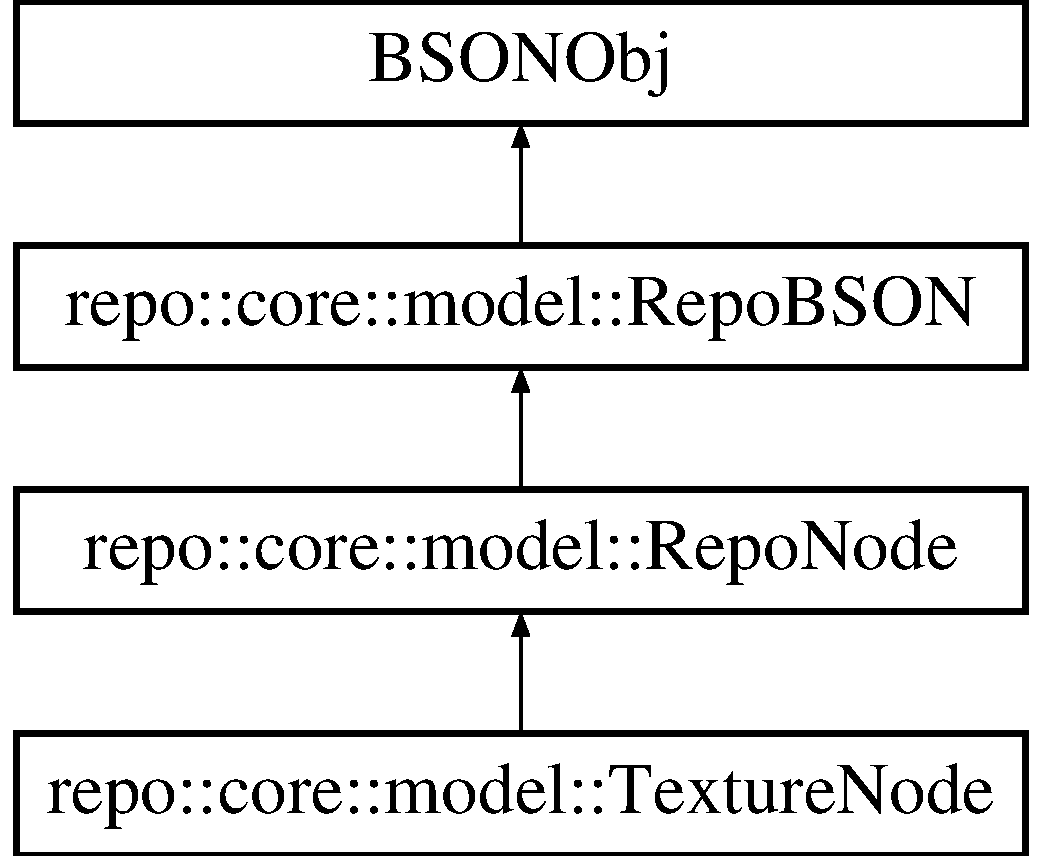
\includegraphics[height=4.000000cm]{classrepo_1_1core_1_1model_1_1_texture_node}
\end{center}
\end{figure}
\subsection*{Public Member Functions}
\begin{DoxyCompactItemize}
\item 
\hyperlink{classrepo_1_1core_1_1model_1_1_texture_node_a87faf55e6621f469e898021fa3a11903}{Texture\+Node} ()
\item 
\hyperlink{classrepo_1_1core_1_1model_1_1_texture_node_a895ddcf97500bebe7a14faa74262f5c5}{Texture\+Node} (\hyperlink{classrepo_1_1core_1_1model_1_1_repo_b_s_o_n}{Repo\+B\+S\+O\+N} bson)
\item 
\hyperlink{classrepo_1_1core_1_1model_1_1_texture_node_ab164fe59d9b100109c26387c2bf69553}{$\sim$\+Texture\+Node} ()
\item 
virtual std\+::string \hyperlink{classrepo_1_1core_1_1model_1_1_texture_node_aaae4c87e4e841d8bddc105e29e759d2a}{get\+Type} () const 
\item 
virtual Node\+Type \hyperlink{classrepo_1_1core_1_1model_1_1_texture_node_a78fadf9b11659cf83c24d367b66a6772}{get\+Type\+As\+Enum} () const 
\item 
virtual bool \hyperlink{classrepo_1_1core_1_1model_1_1_texture_node_acc560eb9f51e63bb83d35e859ee4f4c4}{s\+Equal} (const \hyperlink{classrepo_1_1core_1_1model_1_1_repo_node}{Repo\+Node} \&other) const 
\item 
std\+::vector$<$ char $>$ \hyperlink{classrepo_1_1core_1_1model_1_1_texture_node_a06c5329c625a3b1771d03d955ce5643d}{get\+Raw\+Data} () const 
\item 
\hypertarget{classrepo_1_1core_1_1model_1_1_texture_node_a2dc5fa1285a0a647c6c2f95495b6b4fc}{}std\+::string {\bfseries get\+File\+Extension} () const \label{classrepo_1_1core_1_1model_1_1_texture_node_a2dc5fa1285a0a647c6c2f95495b6b4fc}

\end{DoxyCompactItemize}
\subsection*{Additional Inherited Members}


\subsection{Constructor \& Destructor Documentation}
\hypertarget{classrepo_1_1core_1_1model_1_1_texture_node_a87faf55e6621f469e898021fa3a11903}{}\index{repo\+::core\+::model\+::\+Texture\+Node@{repo\+::core\+::model\+::\+Texture\+Node}!Texture\+Node@{Texture\+Node}}
\index{Texture\+Node@{Texture\+Node}!repo\+::core\+::model\+::\+Texture\+Node@{repo\+::core\+::model\+::\+Texture\+Node}}
\subsubsection[{Texture\+Node}]{\setlength{\rightskip}{0pt plus 5cm}Texture\+Node\+::\+Texture\+Node (
\begin{DoxyParamCaption}
{}
\end{DoxyParamCaption}
)}\label{classrepo_1_1core_1_1model_1_1_texture_node_a87faf55e6621f469e898021fa3a11903}
Default constructor \hypertarget{classrepo_1_1core_1_1model_1_1_texture_node_a895ddcf97500bebe7a14faa74262f5c5}{}\index{repo\+::core\+::model\+::\+Texture\+Node@{repo\+::core\+::model\+::\+Texture\+Node}!Texture\+Node@{Texture\+Node}}
\index{Texture\+Node@{Texture\+Node}!repo\+::core\+::model\+::\+Texture\+Node@{repo\+::core\+::model\+::\+Texture\+Node}}
\subsubsection[{Texture\+Node}]{\setlength{\rightskip}{0pt plus 5cm}Texture\+Node\+::\+Texture\+Node (
\begin{DoxyParamCaption}
\item[{{\bf Repo\+B\+S\+O\+N}}]{bson}
\end{DoxyParamCaption}
)}\label{classrepo_1_1core_1_1model_1_1_texture_node_a895ddcf97500bebe7a14faa74262f5c5}
Construct a \hyperlink{classrepo_1_1core_1_1model_1_1_texture_node}{Texture\+Node} from a \hyperlink{classrepo_1_1core_1_1model_1_1_repo_b_s_o_n}{Repo\+B\+S\+O\+N} object 
\begin{DoxyParams}{Parameters}
{\em \hyperlink{classrepo_1_1core_1_1model_1_1_repo_b_s_o_n}{Repo\+B\+S\+O\+N}} & object \\
\hline
\end{DoxyParams}
\hypertarget{classrepo_1_1core_1_1model_1_1_texture_node_ab164fe59d9b100109c26387c2bf69553}{}\index{repo\+::core\+::model\+::\+Texture\+Node@{repo\+::core\+::model\+::\+Texture\+Node}!````~Texture\+Node@{$\sim$\+Texture\+Node}}
\index{````~Texture\+Node@{$\sim$\+Texture\+Node}!repo\+::core\+::model\+::\+Texture\+Node@{repo\+::core\+::model\+::\+Texture\+Node}}
\subsubsection[{$\sim$\+Texture\+Node}]{\setlength{\rightskip}{0pt plus 5cm}Texture\+Node\+::$\sim$\+Texture\+Node (
\begin{DoxyParamCaption}
{}
\end{DoxyParamCaption}
)}\label{classrepo_1_1core_1_1model_1_1_texture_node_ab164fe59d9b100109c26387c2bf69553}
Default deconstructor 

\subsection{Member Function Documentation}
\hypertarget{classrepo_1_1core_1_1model_1_1_texture_node_a06c5329c625a3b1771d03d955ce5643d}{}\index{repo\+::core\+::model\+::\+Texture\+Node@{repo\+::core\+::model\+::\+Texture\+Node}!get\+Raw\+Data@{get\+Raw\+Data}}
\index{get\+Raw\+Data@{get\+Raw\+Data}!repo\+::core\+::model\+::\+Texture\+Node@{repo\+::core\+::model\+::\+Texture\+Node}}
\subsubsection[{get\+Raw\+Data}]{\setlength{\rightskip}{0pt plus 5cm}std\+::vector$<$ char $>$ Texture\+Node\+::get\+Raw\+Data (
\begin{DoxyParamCaption}
{}
\end{DoxyParamCaption}
) const}\label{classrepo_1_1core_1_1model_1_1_texture_node_a06c5329c625a3b1771d03d955ce5643d}
-\/-\/-\/------ Convenience functions -\/-\/-\/-\/-\/------ Retrieve texture image as raw data \begin{DoxyReturn}{Returns}
returns a pointer to the image (represented as char) 
\end{DoxyReturn}
\hypertarget{classrepo_1_1core_1_1model_1_1_texture_node_aaae4c87e4e841d8bddc105e29e759d2a}{}\index{repo\+::core\+::model\+::\+Texture\+Node@{repo\+::core\+::model\+::\+Texture\+Node}!get\+Type@{get\+Type}}
\index{get\+Type@{get\+Type}!repo\+::core\+::model\+::\+Texture\+Node@{repo\+::core\+::model\+::\+Texture\+Node}}
\subsubsection[{get\+Type}]{\setlength{\rightskip}{0pt plus 5cm}virtual std\+::string repo\+::core\+::model\+::\+Texture\+Node\+::get\+Type (
\begin{DoxyParamCaption}
{}
\end{DoxyParamCaption}
) const\hspace{0.3cm}{\ttfamily [inline]}, {\ttfamily [virtual]}}\label{classrepo_1_1core_1_1model_1_1_texture_node_aaae4c87e4e841d8bddc105e29e759d2a}
Get the type of node \begin{DoxyReturn}{Returns}
returns the type as a string 
\end{DoxyReturn}


Reimplemented from \hyperlink{classrepo_1_1core_1_1model_1_1_repo_node_a4380ba349235b5d9b13b41e41975805e}{repo\+::core\+::model\+::\+Repo\+Node}.

\hypertarget{classrepo_1_1core_1_1model_1_1_texture_node_a78fadf9b11659cf83c24d367b66a6772}{}\index{repo\+::core\+::model\+::\+Texture\+Node@{repo\+::core\+::model\+::\+Texture\+Node}!get\+Type\+As\+Enum@{get\+Type\+As\+Enum}}
\index{get\+Type\+As\+Enum@{get\+Type\+As\+Enum}!repo\+::core\+::model\+::\+Texture\+Node@{repo\+::core\+::model\+::\+Texture\+Node}}
\subsubsection[{get\+Type\+As\+Enum}]{\setlength{\rightskip}{0pt plus 5cm}virtual Node\+Type repo\+::core\+::model\+::\+Texture\+Node\+::get\+Type\+As\+Enum (
\begin{DoxyParamCaption}
{}
\end{DoxyParamCaption}
) const\hspace{0.3cm}{\ttfamily [inline]}, {\ttfamily [virtual]}}\label{classrepo_1_1core_1_1model_1_1_texture_node_a78fadf9b11659cf83c24d367b66a6772}
Get the type of node as an enum \begin{DoxyReturn}{Returns}
returns type as enum. 
\end{DoxyReturn}


Reimplemented from \hyperlink{classrepo_1_1core_1_1model_1_1_repo_node_ad8d5295248dc9beb0b91efb2ce3b61f4}{repo\+::core\+::model\+::\+Repo\+Node}.

\hypertarget{classrepo_1_1core_1_1model_1_1_texture_node_acc560eb9f51e63bb83d35e859ee4f4c4}{}\index{repo\+::core\+::model\+::\+Texture\+Node@{repo\+::core\+::model\+::\+Texture\+Node}!s\+Equal@{s\+Equal}}
\index{s\+Equal@{s\+Equal}!repo\+::core\+::model\+::\+Texture\+Node@{repo\+::core\+::model\+::\+Texture\+Node}}
\subsubsection[{s\+Equal}]{\setlength{\rightskip}{0pt plus 5cm}bool Texture\+Node\+::s\+Equal (
\begin{DoxyParamCaption}
\item[{const {\bf Repo\+Node} \&}]{other}
\end{DoxyParamCaption}
) const\hspace{0.3cm}{\ttfamily [virtual]}}\label{classrepo_1_1core_1_1model_1_1_texture_node_acc560eb9f51e63bb83d35e859ee4f4c4}
Check if the node is semantically equal to another Different node should have a different interpretation of what this means. 
\begin{DoxyParams}{Parameters}
{\em other} & node to compare with \\
\hline
{\em returns} & true if equal, false otherwise \\
\hline
\end{DoxyParams}


Reimplemented from \hyperlink{classrepo_1_1core_1_1model_1_1_repo_node_a7c98830a876ee6516587a8f07c7015a5}{repo\+::core\+::model\+::\+Repo\+Node}.



The documentation for this class was generated from the following files\+:\begin{DoxyCompactItemize}
\item 
C\+:/\+Users/\+Carmen/3\+D Repo/\+Repo/3drepobouncer/bouncer/src/repo/core/model/bson/repo\+\_\+node\+\_\+texture.\+h\item 
C\+:/\+Users/\+Carmen/3\+D Repo/\+Repo/3drepobouncer/bouncer/src/repo/core/model/bson/repo\+\_\+node\+\_\+texture.\+cpp\end{DoxyCompactItemize}

\hypertarget{classrepo_1_1core_1_1model_1_1_transformation_node}{}\section{repo\+:\+:core\+:\+:model\+:\+:Transformation\+Node Class Reference}
\label{classrepo_1_1core_1_1model_1_1_transformation_node}\index{repo\+::core\+::model\+::\+Transformation\+Node@{repo\+::core\+::model\+::\+Transformation\+Node}}
Inheritance diagram for repo\+:\+:core\+:\+:model\+:\+:Transformation\+Node\+:\begin{figure}[H]
\begin{center}
\leavevmode
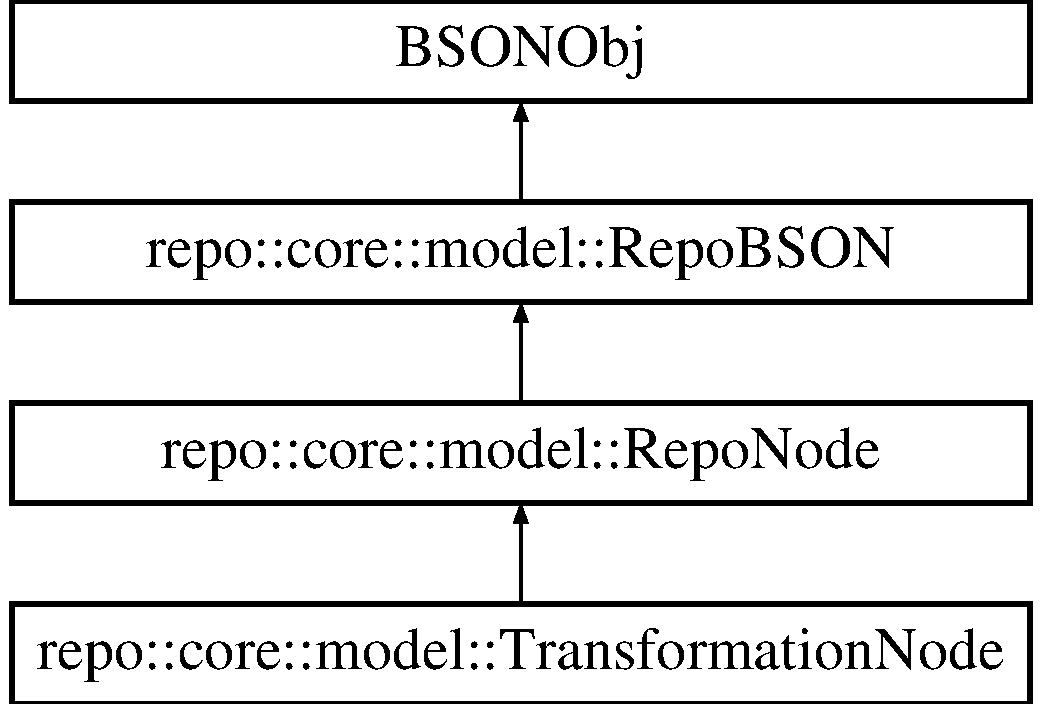
\includegraphics[height=4.000000cm]{classrepo_1_1core_1_1model_1_1_transformation_node}
\end{center}
\end{figure}
\subsection*{Public Member Functions}
\begin{DoxyCompactItemize}
\item 
\hyperlink{classrepo_1_1core_1_1model_1_1_transformation_node_a4ed71fa34f550f4b47c21c8692c9f224}{Transformation\+Node} ()
\item 
\hyperlink{classrepo_1_1core_1_1model_1_1_transformation_node_a67b879ee0759867301de573ff16b8267}{Transformation\+Node} (\hyperlink{classrepo_1_1core_1_1model_1_1_repo_b_s_o_n}{Repo\+B\+S\+O\+N} bson)
\item 
\hyperlink{classrepo_1_1core_1_1model_1_1_transformation_node_a257896cca60b0abb300081a41da68a85}{$\sim$\+Transformation\+Node} ()
\item 
bool \hyperlink{classrepo_1_1core_1_1model_1_1_transformation_node_a60a86aff26b5d47c4aaf1db5bd9b7c74}{is\+Identity} (const float \&eps=10e-\/5) const 
\item 
virtual std\+::string \hyperlink{classrepo_1_1core_1_1model_1_1_transformation_node_a7e0b577dccbdbcab1e833b4da3121e83}{get\+Type} () const 
\item 
virtual Node\+Type \hyperlink{classrepo_1_1core_1_1model_1_1_transformation_node_ae24b2692960c32fed8b8b1ebf732a333}{get\+Type\+As\+Enum} () const 
\item 
virtual bool \hyperlink{classrepo_1_1core_1_1model_1_1_transformation_node_aef0c61c652ac425139a063c5e5c1832b}{position\+Dependant} ()
\item 
virtual bool \hyperlink{classrepo_1_1core_1_1model_1_1_transformation_node_ae580f6d1f6e6d331180ab6bb408f7e66}{s\+Equal} (const \hyperlink{classrepo_1_1core_1_1model_1_1_repo_node}{Repo\+Node} \&other) const 
\item 
virtual \hyperlink{classrepo_1_1core_1_1model_1_1_repo_node}{Repo\+Node} \hyperlink{classrepo_1_1core_1_1model_1_1_transformation_node_ad7ee2c9234712c2c697e06c02b34ed9b}{clone\+And\+Apply\+Transformation} (const std\+::vector$<$ float $>$ \&matrix) const 
\item 
std\+::vector$<$ float $>$ \hyperlink{classrepo_1_1core_1_1model_1_1_transformation_node_ae8f87497de15d3aa0d45298cd0dd32b8}{get\+Trans\+Matrix} (const bool \&row\+Major) const 
\end{DoxyCompactItemize}
\subsection*{Static Public Member Functions}
\begin{DoxyCompactItemize}
\item 
static std\+::vector$<$ std\+::vector$<$ float $>$ $>$ \hyperlink{classrepo_1_1core_1_1model_1_1_transformation_node_ac6723324b4ef9d6c0aacf53572a46d7f}{identity\+Mat} ()
\end{DoxyCompactItemize}
\subsection*{Additional Inherited Members}


\subsection{Constructor \& Destructor Documentation}
\hypertarget{classrepo_1_1core_1_1model_1_1_transformation_node_a4ed71fa34f550f4b47c21c8692c9f224}{}\index{repo\+::core\+::model\+::\+Transformation\+Node@{repo\+::core\+::model\+::\+Transformation\+Node}!Transformation\+Node@{Transformation\+Node}}
\index{Transformation\+Node@{Transformation\+Node}!repo\+::core\+::model\+::\+Transformation\+Node@{repo\+::core\+::model\+::\+Transformation\+Node}}
\subsubsection[{Transformation\+Node}]{\setlength{\rightskip}{0pt plus 5cm}Transformation\+Node\+::\+Transformation\+Node (
\begin{DoxyParamCaption}
{}
\end{DoxyParamCaption}
)}\label{classrepo_1_1core_1_1model_1_1_transformation_node_a4ed71fa34f550f4b47c21c8692c9f224}
Default constructor \hypertarget{classrepo_1_1core_1_1model_1_1_transformation_node_a67b879ee0759867301de573ff16b8267}{}\index{repo\+::core\+::model\+::\+Transformation\+Node@{repo\+::core\+::model\+::\+Transformation\+Node}!Transformation\+Node@{Transformation\+Node}}
\index{Transformation\+Node@{Transformation\+Node}!repo\+::core\+::model\+::\+Transformation\+Node@{repo\+::core\+::model\+::\+Transformation\+Node}}
\subsubsection[{Transformation\+Node}]{\setlength{\rightskip}{0pt plus 5cm}Transformation\+Node\+::\+Transformation\+Node (
\begin{DoxyParamCaption}
\item[{{\bf Repo\+B\+S\+O\+N}}]{bson}
\end{DoxyParamCaption}
)}\label{classrepo_1_1core_1_1model_1_1_transformation_node_a67b879ee0759867301de573ff16b8267}
Construct a \hyperlink{classrepo_1_1core_1_1model_1_1_transformation_node}{Transformation\+Node} from a \hyperlink{classrepo_1_1core_1_1model_1_1_repo_b_s_o_n}{Repo\+B\+S\+O\+N} object 
\begin{DoxyParams}{Parameters}
{\em \hyperlink{classrepo_1_1core_1_1model_1_1_repo_b_s_o_n}{Repo\+B\+S\+O\+N}} & object \\
\hline
\end{DoxyParams}
\hypertarget{classrepo_1_1core_1_1model_1_1_transformation_node_a257896cca60b0abb300081a41da68a85}{}\index{repo\+::core\+::model\+::\+Transformation\+Node@{repo\+::core\+::model\+::\+Transformation\+Node}!````~Transformation\+Node@{$\sim$\+Transformation\+Node}}
\index{````~Transformation\+Node@{$\sim$\+Transformation\+Node}!repo\+::core\+::model\+::\+Transformation\+Node@{repo\+::core\+::model\+::\+Transformation\+Node}}
\subsubsection[{$\sim$\+Transformation\+Node}]{\setlength{\rightskip}{0pt plus 5cm}Transformation\+Node\+::$\sim$\+Transformation\+Node (
\begin{DoxyParamCaption}
{}
\end{DoxyParamCaption}
)}\label{classrepo_1_1core_1_1model_1_1_transformation_node_a257896cca60b0abb300081a41da68a85}
Default deconstructor 

\subsection{Member Function Documentation}
\hypertarget{classrepo_1_1core_1_1model_1_1_transformation_node_ad7ee2c9234712c2c697e06c02b34ed9b}{}\index{repo\+::core\+::model\+::\+Transformation\+Node@{repo\+::core\+::model\+::\+Transformation\+Node}!clone\+And\+Apply\+Transformation@{clone\+And\+Apply\+Transformation}}
\index{clone\+And\+Apply\+Transformation@{clone\+And\+Apply\+Transformation}!repo\+::core\+::model\+::\+Transformation\+Node@{repo\+::core\+::model\+::\+Transformation\+Node}}
\subsubsection[{clone\+And\+Apply\+Transformation}]{\setlength{\rightskip}{0pt plus 5cm}{\bf Repo\+Node} Transformation\+Node\+::clone\+And\+Apply\+Transformation (
\begin{DoxyParamCaption}
\item[{const std\+::vector$<$ float $>$ \&}]{matrix}
\end{DoxyParamCaption}
) const\hspace{0.3cm}{\ttfamily [virtual]}}\label{classrepo_1_1core_1_1model_1_1_transformation_node_ad7ee2c9234712c2c697e06c02b34ed9b}
Create a new object with transformation applied to the node default behaviour is do nothing. Children object needs to override this function to perform their own specific behaviour. 
\begin{DoxyParams}{Parameters}
{\em matrix} & transformation matrix to apply. \\
\hline
\end{DoxyParams}
\begin{DoxyReturn}{Returns}
returns a new object with transformation applied. 
\end{DoxyReturn}


Reimplemented from \hyperlink{classrepo_1_1core_1_1model_1_1_repo_node_ac31acdb9774bce9296cb5005286db83d}{repo\+::core\+::model\+::\+Repo\+Node}.

\hypertarget{classrepo_1_1core_1_1model_1_1_transformation_node_ae8f87497de15d3aa0d45298cd0dd32b8}{}\index{repo\+::core\+::model\+::\+Transformation\+Node@{repo\+::core\+::model\+::\+Transformation\+Node}!get\+Trans\+Matrix@{get\+Trans\+Matrix}}
\index{get\+Trans\+Matrix@{get\+Trans\+Matrix}!repo\+::core\+::model\+::\+Transformation\+Node@{repo\+::core\+::model\+::\+Transformation\+Node}}
\subsubsection[{get\+Trans\+Matrix}]{\setlength{\rightskip}{0pt plus 5cm}std\+::vector$<$ float $>$ Transformation\+Node\+::get\+Trans\+Matrix (
\begin{DoxyParamCaption}
\item[{const bool \&}]{row\+Major}
\end{DoxyParamCaption}
) const}\label{classrepo_1_1core_1_1model_1_1_transformation_node_ae8f87497de15d3aa0d45298cd0dd32b8}
-\/-\/-\/------ Convenience functions -\/-\/-\/-\/-\/------ Get the 4 by 4 transformation matrix 
\begin{DoxyParams}{Parameters}
{\em true} & if row major (row is the fast dimension) \\
\hline
\end{DoxyParams}
\begin{DoxyReturn}{Returns}
returns the 4 by 4 matrix as a vector 
\end{DoxyReturn}
\hypertarget{classrepo_1_1core_1_1model_1_1_transformation_node_a7e0b577dccbdbcab1e833b4da3121e83}{}\index{repo\+::core\+::model\+::\+Transformation\+Node@{repo\+::core\+::model\+::\+Transformation\+Node}!get\+Type@{get\+Type}}
\index{get\+Type@{get\+Type}!repo\+::core\+::model\+::\+Transformation\+Node@{repo\+::core\+::model\+::\+Transformation\+Node}}
\subsubsection[{get\+Type}]{\setlength{\rightskip}{0pt plus 5cm}virtual std\+::string repo\+::core\+::model\+::\+Transformation\+Node\+::get\+Type (
\begin{DoxyParamCaption}
{}
\end{DoxyParamCaption}
) const\hspace{0.3cm}{\ttfamily [inline]}, {\ttfamily [virtual]}}\label{classrepo_1_1core_1_1model_1_1_transformation_node_a7e0b577dccbdbcab1e833b4da3121e83}
Get the type of node \begin{DoxyReturn}{Returns}
returns the type as a string 
\end{DoxyReturn}


Reimplemented from \hyperlink{classrepo_1_1core_1_1model_1_1_repo_node_a4380ba349235b5d9b13b41e41975805e}{repo\+::core\+::model\+::\+Repo\+Node}.

\hypertarget{classrepo_1_1core_1_1model_1_1_transformation_node_ae24b2692960c32fed8b8b1ebf732a333}{}\index{repo\+::core\+::model\+::\+Transformation\+Node@{repo\+::core\+::model\+::\+Transformation\+Node}!get\+Type\+As\+Enum@{get\+Type\+As\+Enum}}
\index{get\+Type\+As\+Enum@{get\+Type\+As\+Enum}!repo\+::core\+::model\+::\+Transformation\+Node@{repo\+::core\+::model\+::\+Transformation\+Node}}
\subsubsection[{get\+Type\+As\+Enum}]{\setlength{\rightskip}{0pt plus 5cm}virtual Node\+Type repo\+::core\+::model\+::\+Transformation\+Node\+::get\+Type\+As\+Enum (
\begin{DoxyParamCaption}
{}
\end{DoxyParamCaption}
) const\hspace{0.3cm}{\ttfamily [inline]}, {\ttfamily [virtual]}}\label{classrepo_1_1core_1_1model_1_1_transformation_node_ae24b2692960c32fed8b8b1ebf732a333}
Get the type of node as an enum \begin{DoxyReturn}{Returns}
returns type as enum. 
\end{DoxyReturn}


Reimplemented from \hyperlink{classrepo_1_1core_1_1model_1_1_repo_node_ad8d5295248dc9beb0b91efb2ce3b61f4}{repo\+::core\+::model\+::\+Repo\+Node}.

\hypertarget{classrepo_1_1core_1_1model_1_1_transformation_node_ac6723324b4ef9d6c0aacf53572a46d7f}{}\index{repo\+::core\+::model\+::\+Transformation\+Node@{repo\+::core\+::model\+::\+Transformation\+Node}!identity\+Mat@{identity\+Mat}}
\index{identity\+Mat@{identity\+Mat}!repo\+::core\+::model\+::\+Transformation\+Node@{repo\+::core\+::model\+::\+Transformation\+Node}}
\subsubsection[{identity\+Mat}]{\setlength{\rightskip}{0pt plus 5cm}std\+::vector$<$ std\+::vector$<$ float $>$ $>$ Transformation\+Node\+::identity\+Mat (
\begin{DoxyParamCaption}
{}
\end{DoxyParamCaption}
)\hspace{0.3cm}{\ttfamily [static]}}\label{classrepo_1_1core_1_1model_1_1_transformation_node_ac6723324b4ef9d6c0aacf53572a46d7f}
Create an Identity matrix \begin{DoxyReturn}{Returns}
returns a 4 by 4 identity matrix 
\end{DoxyReturn}
\hypertarget{classrepo_1_1core_1_1model_1_1_transformation_node_a60a86aff26b5d47c4aaf1db5bd9b7c74}{}\index{repo\+::core\+::model\+::\+Transformation\+Node@{repo\+::core\+::model\+::\+Transformation\+Node}!is\+Identity@{is\+Identity}}
\index{is\+Identity@{is\+Identity}!repo\+::core\+::model\+::\+Transformation\+Node@{repo\+::core\+::model\+::\+Transformation\+Node}}
\subsubsection[{is\+Identity}]{\setlength{\rightskip}{0pt plus 5cm}bool Transformation\+Node\+::is\+Identity (
\begin{DoxyParamCaption}
\item[{const float \&}]{eps = {\ttfamily 10e-\/5}}
\end{DoxyParamCaption}
) const}\label{classrepo_1_1core_1_1model_1_1_transformation_node_a60a86aff26b5d47c4aaf1db5bd9b7c74}
Check if the transformation matrix is the identity matrix This checks with a small epsilon to counter floating point inaccuracies 
\begin{DoxyParams}{Parameters}
{\em eps} & epsilon value for accepting inaccuracies (default 10e-\/5) \\
\hline
\end{DoxyParams}
\begin{DoxyReturn}{Returns}
returns true if it is the identity matrix 
\end{DoxyReturn}
\hypertarget{classrepo_1_1core_1_1model_1_1_transformation_node_aef0c61c652ac425139a063c5e5c1832b}{}\index{repo\+::core\+::model\+::\+Transformation\+Node@{repo\+::core\+::model\+::\+Transformation\+Node}!position\+Dependant@{position\+Dependant}}
\index{position\+Dependant@{position\+Dependant}!repo\+::core\+::model\+::\+Transformation\+Node@{repo\+::core\+::model\+::\+Transformation\+Node}}
\subsubsection[{position\+Dependant}]{\setlength{\rightskip}{0pt plus 5cm}virtual bool repo\+::core\+::model\+::\+Transformation\+Node\+::position\+Dependant (
\begin{DoxyParamCaption}
{}
\end{DoxyParamCaption}
)\hspace{0.3cm}{\ttfamily [inline]}, {\ttfamily [virtual]}}\label{classrepo_1_1core_1_1model_1_1_transformation_node_aef0c61c652ac425139a063c5e5c1832b}
Check if the node is position dependant. i.\+e. if parent transformation is merged onto the node, does the node requre to a transformation applied to it e.\+g. meshes and cameras are position dependant, metadata isn\textquotesingle{}t Default behaviour is false. Position dependant child requires override this function. \begin{DoxyReturn}{Returns}
true if node is position\+Dependant. 
\end{DoxyReturn}


Reimplemented from \hyperlink{classrepo_1_1core_1_1model_1_1_repo_node_aa3e0f98690dc8bfe082d2fc57b904798}{repo\+::core\+::model\+::\+Repo\+Node}.

\hypertarget{classrepo_1_1core_1_1model_1_1_transformation_node_ae580f6d1f6e6d331180ab6bb408f7e66}{}\index{repo\+::core\+::model\+::\+Transformation\+Node@{repo\+::core\+::model\+::\+Transformation\+Node}!s\+Equal@{s\+Equal}}
\index{s\+Equal@{s\+Equal}!repo\+::core\+::model\+::\+Transformation\+Node@{repo\+::core\+::model\+::\+Transformation\+Node}}
\subsubsection[{s\+Equal}]{\setlength{\rightskip}{0pt plus 5cm}bool Transformation\+Node\+::s\+Equal (
\begin{DoxyParamCaption}
\item[{const {\bf Repo\+Node} \&}]{other}
\end{DoxyParamCaption}
) const\hspace{0.3cm}{\ttfamily [virtual]}}\label{classrepo_1_1core_1_1model_1_1_transformation_node_ae580f6d1f6e6d331180ab6bb408f7e66}
Check if the node is semantically equal to another Different node should have a different interpretation of what this means. 
\begin{DoxyParams}{Parameters}
{\em other} & node to compare with \\
\hline
{\em returns} & true if equal, false otherwise \\
\hline
\end{DoxyParams}


Reimplemented from \hyperlink{classrepo_1_1core_1_1model_1_1_repo_node_a7c98830a876ee6516587a8f07c7015a5}{repo\+::core\+::model\+::\+Repo\+Node}.



The documentation for this class was generated from the following files\+:\begin{DoxyCompactItemize}
\item 
C\+:/\+Users/\+Carmen/3\+D Repo/\+Repo/3drepobouncer/bouncer/src/repo/core/model/bson/repo\+\_\+node\+\_\+transformation.\+h\item 
C\+:/\+Users/\+Carmen/3\+D Repo/\+Repo/3drepobouncer/bouncer/src/repo/core/model/bson/repo\+\_\+node\+\_\+transformation.\+cpp\end{DoxyCompactItemize}

\hypertarget{classrepo_1_1manipulator_1_1modeloptimizer_1_1_transformation_reduction_optimizer}{}\section{repo\+:\+:manipulator\+:\+:modeloptimizer\+:\+:Transformation\+Reduction\+Optimizer Class Reference}
\label{classrepo_1_1manipulator_1_1modeloptimizer_1_1_transformation_reduction_optimizer}\index{repo\+::manipulator\+::modeloptimizer\+::\+Transformation\+Reduction\+Optimizer@{repo\+::manipulator\+::modeloptimizer\+::\+Transformation\+Reduction\+Optimizer}}
Inheritance diagram for repo\+:\+:manipulator\+:\+:modeloptimizer\+:\+:Transformation\+Reduction\+Optimizer\+:\begin{figure}[H]
\begin{center}
\leavevmode
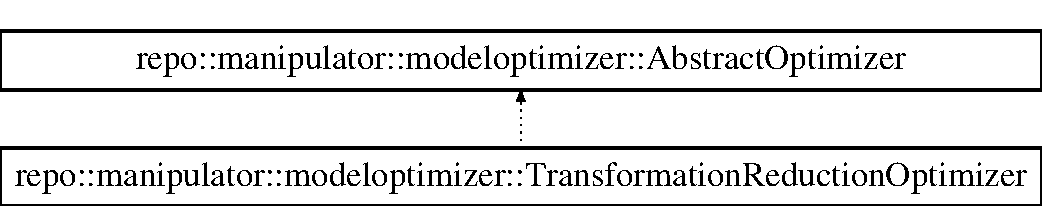
\includegraphics[height=2.000000cm]{classrepo_1_1manipulator_1_1modeloptimizer_1_1_transformation_reduction_optimizer}
\end{center}
\end{figure}
\subsection*{Public Member Functions}
\begin{DoxyCompactItemize}
\item 
\hyperlink{classrepo_1_1manipulator_1_1modeloptimizer_1_1_transformation_reduction_optimizer_aea2109a4102521b4d627356c004daad3}{Transformation\+Reduction\+Optimizer} (const bool strict\+Mode=false)
\item 
virtual \hyperlink{classrepo_1_1manipulator_1_1modeloptimizer_1_1_transformation_reduction_optimizer_a79f21ae816e937b6e3a3c9ceacb7b29f}{$\sim$\+Transformation\+Reduction\+Optimizer} ()
\item 
virtual bool \hyperlink{classrepo_1_1manipulator_1_1modeloptimizer_1_1_transformation_reduction_optimizer_ab1e06e1810e27b99030cf1d86c1b4e06}{apply} (\hyperlink{classrepo_1_1core_1_1model_1_1_repo_scene}{repo\+::core\+::model\+::\+Repo\+Scene} $\ast$scene)
\end{DoxyCompactItemize}


\subsection{Constructor \& Destructor Documentation}
\hypertarget{classrepo_1_1manipulator_1_1modeloptimizer_1_1_transformation_reduction_optimizer_aea2109a4102521b4d627356c004daad3}{}\index{repo\+::manipulator\+::modeloptimizer\+::\+Transformation\+Reduction\+Optimizer@{repo\+::manipulator\+::modeloptimizer\+::\+Transformation\+Reduction\+Optimizer}!Transformation\+Reduction\+Optimizer@{Transformation\+Reduction\+Optimizer}}
\index{Transformation\+Reduction\+Optimizer@{Transformation\+Reduction\+Optimizer}!repo\+::manipulator\+::modeloptimizer\+::\+Transformation\+Reduction\+Optimizer@{repo\+::manipulator\+::modeloptimizer\+::\+Transformation\+Reduction\+Optimizer}}
\subsubsection[{Transformation\+Reduction\+Optimizer}]{\setlength{\rightskip}{0pt plus 5cm}Transformation\+Reduction\+Optimizer\+::\+Transformation\+Reduction\+Optimizer (
\begin{DoxyParamCaption}
\item[{const bool}]{strict\+Mode = {\ttfamily false}}
\end{DoxyParamCaption}
)}\label{classrepo_1_1manipulator_1_1modeloptimizer_1_1_transformation_reduction_optimizer_aea2109a4102521b4d627356c004daad3}
Default constructor if strict\+Mode is set to true, only single trans to single meta/mesh will be optimised \hypertarget{classrepo_1_1manipulator_1_1modeloptimizer_1_1_transformation_reduction_optimizer_a79f21ae816e937b6e3a3c9ceacb7b29f}{}\index{repo\+::manipulator\+::modeloptimizer\+::\+Transformation\+Reduction\+Optimizer@{repo\+::manipulator\+::modeloptimizer\+::\+Transformation\+Reduction\+Optimizer}!````~Transformation\+Reduction\+Optimizer@{$\sim$\+Transformation\+Reduction\+Optimizer}}
\index{````~Transformation\+Reduction\+Optimizer@{$\sim$\+Transformation\+Reduction\+Optimizer}!repo\+::manipulator\+::modeloptimizer\+::\+Transformation\+Reduction\+Optimizer@{repo\+::manipulator\+::modeloptimizer\+::\+Transformation\+Reduction\+Optimizer}}
\subsubsection[{$\sim$\+Transformation\+Reduction\+Optimizer}]{\setlength{\rightskip}{0pt plus 5cm}Transformation\+Reduction\+Optimizer\+::$\sim$\+Transformation\+Reduction\+Optimizer (
\begin{DoxyParamCaption}
{}
\end{DoxyParamCaption}
)\hspace{0.3cm}{\ttfamily [virtual]}}\label{classrepo_1_1manipulator_1_1modeloptimizer_1_1_transformation_reduction_optimizer_a79f21ae816e937b6e3a3c9ceacb7b29f}
Default deconstructor 

\subsection{Member Function Documentation}
\hypertarget{classrepo_1_1manipulator_1_1modeloptimizer_1_1_transformation_reduction_optimizer_ab1e06e1810e27b99030cf1d86c1b4e06}{}\index{repo\+::manipulator\+::modeloptimizer\+::\+Transformation\+Reduction\+Optimizer@{repo\+::manipulator\+::modeloptimizer\+::\+Transformation\+Reduction\+Optimizer}!apply@{apply}}
\index{apply@{apply}!repo\+::manipulator\+::modeloptimizer\+::\+Transformation\+Reduction\+Optimizer@{repo\+::manipulator\+::modeloptimizer\+::\+Transformation\+Reduction\+Optimizer}}
\subsubsection[{apply}]{\setlength{\rightskip}{0pt plus 5cm}bool Transformation\+Reduction\+Optimizer\+::apply (
\begin{DoxyParamCaption}
\item[{{\bf repo\+::core\+::model\+::\+Repo\+Scene} $\ast$}]{scene}
\end{DoxyParamCaption}
)\hspace{0.3cm}{\ttfamily [virtual]}}\label{classrepo_1_1manipulator_1_1modeloptimizer_1_1_transformation_reduction_optimizer_ab1e06e1810e27b99030cf1d86c1b4e06}
Apply optimisation on the given repo\+Scene 
\begin{DoxyParams}{Parameters}
{\em scene} & takes in a repo\+Scene to optimise \\
\hline
\end{DoxyParams}
\begin{DoxyReturn}{Returns}
returns true upon success 
\end{DoxyReturn}


Implements \hyperlink{classrepo_1_1manipulator_1_1modeloptimizer_1_1_abstract_optimizer_a38e98344c1d3c66fbea8adae41dc6cb1}{repo\+::manipulator\+::modeloptimizer\+::\+Abstract\+Optimizer}.



The documentation for this class was generated from the following files\+:\begin{DoxyCompactItemize}
\item 
C\+:/\+Users/\+Carmen/3\+D Repo/\+Repo/3drepobouncer/bouncer/src/repo/manipulator/modeloptimizer/repo\+\_\+optimizer\+\_\+trans\+\_\+reduction.\+h\item 
C\+:/\+Users/\+Carmen/3\+D Repo/\+Repo/3drepobouncer/bouncer/src/repo/manipulator/modeloptimizer/repo\+\_\+optimizer\+\_\+trans\+\_\+reduction.\+cpp\end{DoxyCompactItemize}

\hypertarget{classrepo_1_1manipulator_1_1modelconvertor_1_1_web_model_export}{}\section{repo\+:\+:manipulator\+:\+:modelconvertor\+:\+:Web\+Model\+Export Class Reference}
\label{classrepo_1_1manipulator_1_1modelconvertor_1_1_web_model_export}\index{repo\+::manipulator\+::modelconvertor\+::\+Web\+Model\+Export@{repo\+::manipulator\+::modelconvertor\+::\+Web\+Model\+Export}}
Inheritance diagram for repo\+:\+:manipulator\+:\+:modelconvertor\+:\+:Web\+Model\+Export\+:\begin{figure}[H]
\begin{center}
\leavevmode
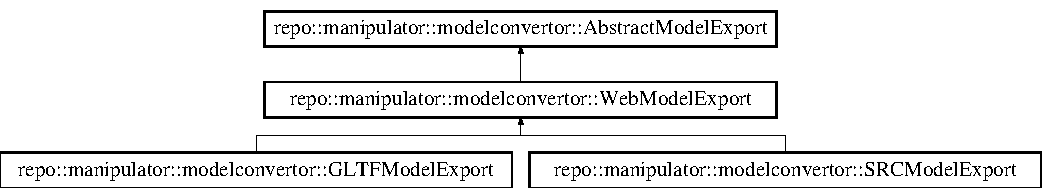
\includegraphics[height=2.507463cm]{classrepo_1_1manipulator_1_1modelconvertor_1_1_web_model_export}
\end{center}
\end{figure}
\subsection*{Public Member Functions}
\begin{DoxyCompactItemize}
\item 
\hyperlink{classrepo_1_1manipulator_1_1modelconvertor_1_1_web_model_export_a26b2b03d3e9b1dd659058f8c21f7355d}{Web\+Model\+Export} (const \hyperlink{classrepo_1_1core_1_1model_1_1_repo_scene}{repo\+::core\+::model\+::\+Repo\+Scene} $\ast$scene)
\item 
virtual \hyperlink{classrepo_1_1manipulator_1_1modelconvertor_1_1_web_model_export_a10097ae71b25979330a9a8e5ad403e55}{$\sim$\+Web\+Model\+Export} ()
\item 
virtual bool \hyperlink{classrepo_1_1manipulator_1_1modelconvertor_1_1_web_model_export_a7ce7f209d57bf5cd48499cf3dbbb25d0}{export\+To\+File} (const std\+::string \&file\+Path)
\item 
virtual \hyperlink{structrepo__web__buffers__t}{repo\+\_\+web\+\_\+buffers\+\_\+t} \hyperlink{classrepo_1_1manipulator_1_1modelconvertor_1_1_web_model_export_ad9e20343a2e8a21fb9de2e89ba14bf05}{get\+All\+Files\+Exported\+As\+Buffer} () const =0
\item 
virtual std\+::unordered\+\_\+map$<$ std\+::string, std\+::vector$<$ uint8\+\_\+t $>$ $>$ \hyperlink{classrepo_1_1manipulator_1_1modelconvertor_1_1_web_model_export_afdbd1aa2c77d6493c038cbd52ebcf185}{get\+J\+S\+O\+N\+Files\+As\+Buffer} () const 
\item 
std\+::unordered\+\_\+map$<$ std\+::string, std\+::vector$<$ uint8\+\_\+t $>$ $>$ \hyperlink{classrepo_1_1manipulator_1_1modelconvertor_1_1_web_model_export_acde7b100e2cd2654853a20c0e39304a6}{get\+X3\+D\+Files\+As\+Buffer} () const 
\item 
bool \hyperlink{classrepo_1_1manipulator_1_1modelconvertor_1_1_web_model_export_ac284fe40fa97587feb44e9e2fb2a7b15}{is\+Ok} () const 
\end{DoxyCompactItemize}
\subsection*{Static Public Member Functions}
\begin{DoxyCompactItemize}
\item 
static std\+::string \hyperlink{classrepo_1_1manipulator_1_1modelconvertor_1_1_web_model_export_af6a4e5186a24090b1b7ee48cbdda0ce9}{get\+Supported\+Formats} ()
\end{DoxyCompactItemize}
\subsection*{Protected Attributes}
\begin{DoxyCompactItemize}
\item 
\hypertarget{classrepo_1_1manipulator_1_1modelconvertor_1_1_web_model_export_a72e7693f58cff85bc1aeffeed5783b4e}{}bool {\bfseries convert\+Success}\label{classrepo_1_1manipulator_1_1modelconvertor_1_1_web_model_export_a72e7693f58cff85bc1aeffeed5783b4e}

\item 
\hypertarget{classrepo_1_1manipulator_1_1modelconvertor_1_1_web_model_export_a63ff812eb4ab1186b9b3ea65b5fb5727}{}\hyperlink{classrepo_1_1core_1_1model_1_1_repo_scene_aefcacd6eb4c7774ac1bfe3a6b223337c}{repo\+::core\+::model\+::\+Repo\+Scene\+::\+Graph\+Type} {\bfseries g\+Type}\label{classrepo_1_1manipulator_1_1modelconvertor_1_1_web_model_export_a63ff812eb4ab1186b9b3ea65b5fb5727}

\item 
\hypertarget{classrepo_1_1manipulator_1_1modelconvertor_1_1_web_model_export_a0adc529948d18959652955e5de28d2ab}{}std\+::unordered\+\_\+map$<$ std\+::string, \hyperlink{classrepo_1_1lib_1_1_property_tree}{repo\+::lib\+::\+Property\+Tree} $>$ {\bfseries trees}\label{classrepo_1_1manipulator_1_1modelconvertor_1_1_web_model_export_a0adc529948d18959652955e5de28d2ab}

\item 
\hypertarget{classrepo_1_1manipulator_1_1modelconvertor_1_1_web_model_export_a56ad22341ac91a135104b3ee666623e0}{}std\+::unordered\+\_\+map$<$ std\+::string, std\+::vector$<$ uint8\+\_\+t $>$ $>$ {\bfseries x3d\+Bufs}\label{classrepo_1_1manipulator_1_1modelconvertor_1_1_web_model_export_a56ad22341ac91a135104b3ee666623e0}

\item 
\hypertarget{classrepo_1_1manipulator_1_1modelconvertor_1_1_web_model_export_a255c9dc7ba9db65a72c716015ab855b7}{}std\+::unordered\+\_\+map$<$ std\+::string, \hyperlink{classrepo_1_1lib_1_1_property_tree}{repo\+::lib\+::\+Property\+Tree} $>$ {\bfseries json\+Trees}\label{classrepo_1_1manipulator_1_1modelconvertor_1_1_web_model_export_a255c9dc7ba9db65a72c716015ab855b7}

\end{DoxyCompactItemize}


\subsection{Constructor \& Destructor Documentation}
\hypertarget{classrepo_1_1manipulator_1_1modelconvertor_1_1_web_model_export_a26b2b03d3e9b1dd659058f8c21f7355d}{}\index{repo\+::manipulator\+::modelconvertor\+::\+Web\+Model\+Export@{repo\+::manipulator\+::modelconvertor\+::\+Web\+Model\+Export}!Web\+Model\+Export@{Web\+Model\+Export}}
\index{Web\+Model\+Export@{Web\+Model\+Export}!repo\+::manipulator\+::modelconvertor\+::\+Web\+Model\+Export@{repo\+::manipulator\+::modelconvertor\+::\+Web\+Model\+Export}}
\subsubsection[{Web\+Model\+Export}]{\setlength{\rightskip}{0pt plus 5cm}Web\+Model\+Export\+::\+Web\+Model\+Export (
\begin{DoxyParamCaption}
\item[{const {\bf repo\+::core\+::model\+::\+Repo\+Scene} $\ast$}]{scene}
\end{DoxyParamCaption}
)}\label{classrepo_1_1manipulator_1_1modelconvertor_1_1_web_model_export_a26b2b03d3e9b1dd659058f8c21f7355d}
Default Constructor, export model with default settings 
\begin{DoxyParams}{Parameters}
{\em scene} & repo scene to convert \\
\hline
\end{DoxyParams}
\hypertarget{classrepo_1_1manipulator_1_1modelconvertor_1_1_web_model_export_a10097ae71b25979330a9a8e5ad403e55}{}\index{repo\+::manipulator\+::modelconvertor\+::\+Web\+Model\+Export@{repo\+::manipulator\+::modelconvertor\+::\+Web\+Model\+Export}!````~Web\+Model\+Export@{$\sim$\+Web\+Model\+Export}}
\index{````~Web\+Model\+Export@{$\sim$\+Web\+Model\+Export}!repo\+::manipulator\+::modelconvertor\+::\+Web\+Model\+Export@{repo\+::manipulator\+::modelconvertor\+::\+Web\+Model\+Export}}
\subsubsection[{$\sim$\+Web\+Model\+Export}]{\setlength{\rightskip}{0pt plus 5cm}Web\+Model\+Export\+::$\sim$\+Web\+Model\+Export (
\begin{DoxyParamCaption}
{}
\end{DoxyParamCaption}
)\hspace{0.3cm}{\ttfamily [virtual]}}\label{classrepo_1_1manipulator_1_1modelconvertor_1_1_web_model_export_a10097ae71b25979330a9a8e5ad403e55}
Default Destructor 

\subsection{Member Function Documentation}
\hypertarget{classrepo_1_1manipulator_1_1modelconvertor_1_1_web_model_export_a7ce7f209d57bf5cd48499cf3dbbb25d0}{}\index{repo\+::manipulator\+::modelconvertor\+::\+Web\+Model\+Export@{repo\+::manipulator\+::modelconvertor\+::\+Web\+Model\+Export}!export\+To\+File@{export\+To\+File}}
\index{export\+To\+File@{export\+To\+File}!repo\+::manipulator\+::modelconvertor\+::\+Web\+Model\+Export@{repo\+::manipulator\+::modelconvertor\+::\+Web\+Model\+Export}}
\subsubsection[{export\+To\+File}]{\setlength{\rightskip}{0pt plus 5cm}bool Web\+Model\+Export\+::export\+To\+File (
\begin{DoxyParamCaption}
\item[{const std\+::string \&}]{file\+Path}
\end{DoxyParamCaption}
)\hspace{0.3cm}{\ttfamily [virtual]}}\label{classrepo_1_1manipulator_1_1modelconvertor_1_1_web_model_export_a7ce7f209d57bf5cd48499cf3dbbb25d0}
Export the repo scene graph to file 
\begin{DoxyParams}{Parameters}
{\em file\+Path} & path to destination file \\
\hline
\end{DoxyParams}
\begin{DoxyReturn}{Returns}
returns true upon success 
\end{DoxyReturn}


Implements \hyperlink{classrepo_1_1manipulator_1_1modelconvertor_1_1_abstract_model_export_a305f2967d8112c5417b80fd3e8b8902a}{repo\+::manipulator\+::modelconvertor\+::\+Abstract\+Model\+Export}.

\hypertarget{classrepo_1_1manipulator_1_1modelconvertor_1_1_web_model_export_ad9e20343a2e8a21fb9de2e89ba14bf05}{}\index{repo\+::manipulator\+::modelconvertor\+::\+Web\+Model\+Export@{repo\+::manipulator\+::modelconvertor\+::\+Web\+Model\+Export}!get\+All\+Files\+Exported\+As\+Buffer@{get\+All\+Files\+Exported\+As\+Buffer}}
\index{get\+All\+Files\+Exported\+As\+Buffer@{get\+All\+Files\+Exported\+As\+Buffer}!repo\+::manipulator\+::modelconvertor\+::\+Web\+Model\+Export@{repo\+::manipulator\+::modelconvertor\+::\+Web\+Model\+Export}}
\subsubsection[{get\+All\+Files\+Exported\+As\+Buffer}]{\setlength{\rightskip}{0pt plus 5cm}virtual {\bf repo\+\_\+web\+\_\+buffers\+\_\+t} repo\+::manipulator\+::modelconvertor\+::\+Web\+Model\+Export\+::get\+All\+Files\+Exported\+As\+Buffer (
\begin{DoxyParamCaption}
{}
\end{DoxyParamCaption}
) const\hspace{0.3cm}{\ttfamily [pure virtual]}}\label{classrepo_1_1manipulator_1_1modelconvertor_1_1_web_model_export_ad9e20343a2e8a21fb9de2e89ba14bf05}
Export all necessary files as buffers \begin{DoxyReturn}{Returns}
returns a repo\+\_\+src\+\_\+export\+\_\+t containing all files needed for this model to be rendered 
\end{DoxyReturn}


Implemented in \hyperlink{classrepo_1_1manipulator_1_1modelconvertor_1_1_s_r_c_model_export_aabc41be1f3f75ab3cba44df16e40850e}{repo\+::manipulator\+::modelconvertor\+::\+S\+R\+C\+Model\+Export}, and \hyperlink{classrepo_1_1manipulator_1_1modelconvertor_1_1_g_l_t_f_model_export_af46ede52b996784ab8b7ff15977d186d}{repo\+::manipulator\+::modelconvertor\+::\+G\+L\+T\+F\+Model\+Export}.

\hypertarget{classrepo_1_1manipulator_1_1modelconvertor_1_1_web_model_export_afdbd1aa2c77d6493c038cbd52ebcf185}{}\index{repo\+::manipulator\+::modelconvertor\+::\+Web\+Model\+Export@{repo\+::manipulator\+::modelconvertor\+::\+Web\+Model\+Export}!get\+J\+S\+O\+N\+Files\+As\+Buffer@{get\+J\+S\+O\+N\+Files\+As\+Buffer}}
\index{get\+J\+S\+O\+N\+Files\+As\+Buffer@{get\+J\+S\+O\+N\+Files\+As\+Buffer}!repo\+::manipulator\+::modelconvertor\+::\+Web\+Model\+Export@{repo\+::manipulator\+::modelconvertor\+::\+Web\+Model\+Export}}
\subsubsection[{get\+J\+S\+O\+N\+Files\+As\+Buffer}]{\setlength{\rightskip}{0pt plus 5cm}std\+::unordered\+\_\+map$<$ std\+::string, std\+::vector$<$ uint8\+\_\+t $>$ $>$ Web\+Model\+Export\+::get\+J\+S\+O\+N\+Files\+As\+Buffer (
\begin{DoxyParamCaption}
{}
\end{DoxyParamCaption}
) const\hspace{0.3cm}{\ttfamily [virtual]}}\label{classrepo_1_1manipulator_1_1modelconvertor_1_1_web_model_export_afdbd1aa2c77d6493c038cbd52ebcf185}
Return the J\+S\+O\+N file as raw bytes buffer returns an empty map if the export has failed \hypertarget{classrepo_1_1manipulator_1_1modelconvertor_1_1_web_model_export_af6a4e5186a24090b1b7ee48cbdda0ce9}{}\index{repo\+::manipulator\+::modelconvertor\+::\+Web\+Model\+Export@{repo\+::manipulator\+::modelconvertor\+::\+Web\+Model\+Export}!get\+Supported\+Formats@{get\+Supported\+Formats}}
\index{get\+Supported\+Formats@{get\+Supported\+Formats}!repo\+::manipulator\+::modelconvertor\+::\+Web\+Model\+Export@{repo\+::manipulator\+::modelconvertor\+::\+Web\+Model\+Export}}
\subsubsection[{get\+Supported\+Formats}]{\setlength{\rightskip}{0pt plus 5cm}std\+::string Web\+Model\+Export\+::get\+Supported\+Formats (
\begin{DoxyParamCaption}
{}
\end{DoxyParamCaption}
)\hspace{0.3cm}{\ttfamily [static]}}\label{classrepo_1_1manipulator_1_1modelconvertor_1_1_web_model_export_af6a4e5186a24090b1b7ee48cbdda0ce9}
Get supported file formats for this exporter \hypertarget{classrepo_1_1manipulator_1_1modelconvertor_1_1_web_model_export_acde7b100e2cd2654853a20c0e39304a6}{}\index{repo\+::manipulator\+::modelconvertor\+::\+Web\+Model\+Export@{repo\+::manipulator\+::modelconvertor\+::\+Web\+Model\+Export}!get\+X3\+D\+Files\+As\+Buffer@{get\+X3\+D\+Files\+As\+Buffer}}
\index{get\+X3\+D\+Files\+As\+Buffer@{get\+X3\+D\+Files\+As\+Buffer}!repo\+::manipulator\+::modelconvertor\+::\+Web\+Model\+Export@{repo\+::manipulator\+::modelconvertor\+::\+Web\+Model\+Export}}
\subsubsection[{get\+X3\+D\+Files\+As\+Buffer}]{\setlength{\rightskip}{0pt plus 5cm}std\+::unordered\+\_\+map$<$std\+::string, std\+::vector$<$uint8\+\_\+t$>$ $>$ repo\+::manipulator\+::modelconvertor\+::\+Web\+Model\+Export\+::get\+X3\+D\+Files\+As\+Buffer (
\begin{DoxyParamCaption}
{}
\end{DoxyParamCaption}
) const\hspace{0.3cm}{\ttfamily [inline]}}\label{classrepo_1_1manipulator_1_1modelconvertor_1_1_web_model_export_acde7b100e2cd2654853a20c0e39304a6}
Return the X3\+D file as raw bytes buffer returns an empty map if the export has failed \hypertarget{classrepo_1_1manipulator_1_1modelconvertor_1_1_web_model_export_ac284fe40fa97587feb44e9e2fb2a7b15}{}\index{repo\+::manipulator\+::modelconvertor\+::\+Web\+Model\+Export@{repo\+::manipulator\+::modelconvertor\+::\+Web\+Model\+Export}!is\+Ok@{is\+Ok}}
\index{is\+Ok@{is\+Ok}!repo\+::manipulator\+::modelconvertor\+::\+Web\+Model\+Export@{repo\+::manipulator\+::modelconvertor\+::\+Web\+Model\+Export}}
\subsubsection[{is\+Ok}]{\setlength{\rightskip}{0pt plus 5cm}bool repo\+::manipulator\+::modelconvertor\+::\+Web\+Model\+Export\+::is\+Ok (
\begin{DoxyParamCaption}
{}
\end{DoxyParamCaption}
) const\hspace{0.3cm}{\ttfamily [inline]}}\label{classrepo_1_1manipulator_1_1modelconvertor_1_1_web_model_export_ac284fe40fa97587feb44e9e2fb2a7b15}
Returns the status of the converter, whether it has successfully converted the model \begin{DoxyReturn}{Returns}
returns true if success 
\end{DoxyReturn}


The documentation for this class was generated from the following files\+:\begin{DoxyCompactItemize}
\item 
C\+:/\+Users/\+Carmen/3\+D Repo/\+Repo/3drepobouncer/bouncer/src/repo/manipulator/modelconvertor/export/repo\+\_\+model\+\_\+export\+\_\+web.\+h\item 
C\+:/\+Users/\+Carmen/3\+D Repo/\+Repo/3drepobouncer/bouncer/src/repo/manipulator/modelconvertor/export/repo\+\_\+model\+\_\+export\+\_\+web.\+cpp\end{DoxyCompactItemize}

%--- End generated contents ---

% Index
\backmatter
\newpage
\phantomsection
\clearemptydoublepage
\addcontentsline{toc}{chapter}{Index}
\printindex

\end{document}
